\documentclass[spanish,notitlepage,letterpaper]{report} 
\usepackage{graphicx}
\usepackage{amsmath}
\usepackage[spanish]{babel}
\usepackage[ansinew]{inputenc}
\usepackage{fancyhdr}
\usepackage[dvipsnames]{xcolor}
\usepackage{mdframed}
\usepackage[colorlinks=true,urlcolor=blue,linkcolor=blue]{hyperref}
\usepackage{amsfonts}
\usepackage{amssymb}
\usepackage{dsfont}
\usepackage{mathtools}
\usepackage{draftwatermark}
\usepackage{wallpaper}
\usepackage{xcolor}
\usepackage[top=2cm, bottom=2cm, outer=0cm, inner=0cm]{geometry}
\usepackage{makeidx}
\usepackage{color}
\definecolor{labelcolor}{RGB}{100,0,0}
\usepackage[Lenny]{fncychap}
\SetWatermarkText{Borrador Preliminar}
\SetWatermarkScale{3.5}
\pagestyle{fancy} 
\rhead{} 
\chead{} 
\lfoot{} 
\cfoot{} 
\rfoot{\thepage} \voffset = -0.25in \textheight= 8.0in \textwidth = 6.5in \oddsidemargin = 0.in \headheight = 20pt \headwidth = 6.5in \renewcommand{\headrulewidth}{0.5pt}
\renewcommand{\footrulewidth}{0,5pt}
\makeindex



\begin{document}

\thispagestyle{empty}
%\pagestyle{empty}
%\ThisTileWallPaper{\paperwidth}{\paperheight}{VOLUMEN_1/00_Portada/generalrelativity.jpg}
\vspace{2cm}

\begin{figure}
\centering

\includegraphics[width=1.0\textwidth]{VOLUMEN_1/00_Portada/letras1}
\end{figure}

\begin{figure}
\centering

\includegraphics[width=1.0\textwidth]{VOLUMEN_1/00_Portada/letras2}
\end{figure}

\begin{figure}
\centering
\vspace{0.5cm}
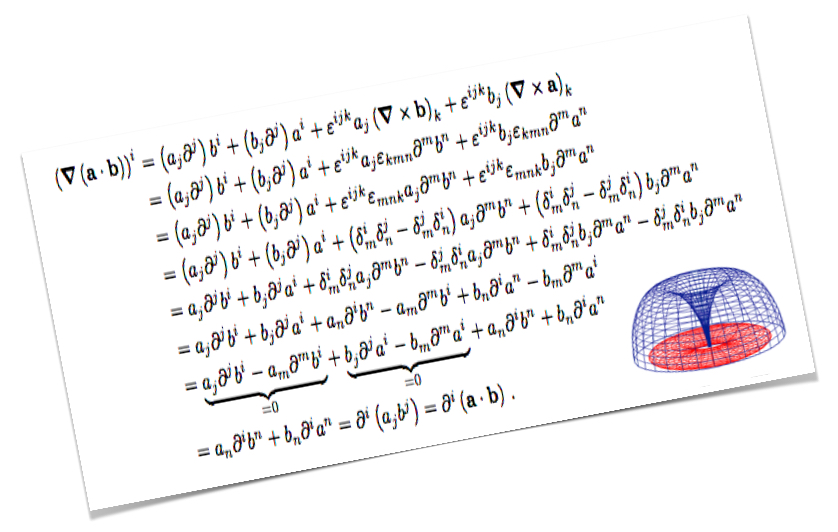
\includegraphics[width=1.0\textwidth]{VOLUMEN_1/00_Portada/figura}
\end{figure}

%%%%%%%%%%%%%%%%%
\begin{figure}[ht]
\begin{minipage}{16.0cm}
\end{minipage} \hfill 
\begin{minipage}{4.0cm} 
\vspace{0.8cm}

\includegraphics[height=1.3in,width=1.8in]{VOLUMEN_1/00_Portada/letras3}
\end{minipage}
\end{figure}
%%%%%%%%%%%%%%%%%







\setcounter{page}{1}
\pagenumbering{roman}
\title{\Huge{\textbf{Matem�ticas Avanzadas:} \\ de los espacios lineales al an�lisis vectorial, \\ con aplicaciones en Maxima}}
\author{
\textbf{H. Hern�ndez} \\ 
\textit{Departamento de F�sica, Facultad de Ciencias, }\\
\textit{Universidad de Los Andes, M�rida-Venezuela} \\ \\
\textbf{L. A. N��ez} \\ 
\textit{Escuela de F�sica, Facultad de Ciencias, }\\
\textit{Universidad Industrial de Santander, Bucaramanga-Colombia} 
}
\maketitle

\tableofcontents


\chapter*{Introducci\'on}
\setcounter{page}{1}
\pagenumbering{arabic}
Como toda obra, el contenido de este libro tuvo como motivaci�n inicial la insatisfacci�n con lo que estaba disponible y esa necesidad de discutir un conjunto de conceptos con el matiz personal de los autores. A lo largo de casi 10 a�os se fue dibujando esa ruta, donde confluyen: una presentaci�n abstracta, una herramienta de c�lculo algebraico y variados ejemplos de aplicaci�n proveniente de la m�s diversas �reas.  Hemos tratado de mostrar que los conceptos abstractos son �tiles porque engloban, bajo un mismo enfoque, una multiplicidad de aplicaciones que normalmente las percibimos aisladas.

Existe, desde hace mucho tiempo,  cierta resistencia en los Departamentos de F�sica en incluir en sus programas de docencia cursos para la ense�anza de herramientas de computaci�n cient�fica y c�lculo num�rico, tal vez debido a los altos costos de la mayor�a de estos programas, casi todos comerciales. Pensamos que la utilizaci�n  de herramientas computacionales enriquece enormemente el aprendizaje de los estudiantes ya que los ense�an a abordar los problemas desde diferentes puntos de vista, les ayuda a familiarizarse con determinados lenguajes de programaci�n y los incentiva a desarrollar sus propias t�cnicas de c�lculo.

Hemos decidido utilizar un sistema de computaci�n algebraico de domino p�blico (o software libre) como {\bf Maxima}  porque estos programas  tienen la capacidad de ofrecer al estudiante  toda una gama de herramientas de c�lculo simb�lico, num�rico y de visualizaci�n de muy alto rendimiento. {\bf Maxima} es un programa que no requiere conocimientos previos de lenguajes de programaci�n pero permitir� que el estudiante se familiarice con la sintaxis de programaci�n y la transici�n a los lenguajes del tipo Fortran, C, o Python ser� mas sencilla. 

Los contenidos que aqu� presentamos han sido utilizados en cursos de M�todos Matem�ticos para estudiantes de pregrado en F�sica de la Universidad de los Andes (M�rida-Venezuela) y m�s recientemente  en los cursos de pregrado y posgrado para estudiantes en F�sica e Ingenier�as en la Universidad Industrial de Santander (Bucaramanga-Colombia). 






\chapter{Los vectores de siempre}
\section*{La ruta de este cap�tulo}
Suponemos que los estudiantes se acercan a estas notas, no solo conociendo algunos t�rminos sino siendo capaces de buscar muchos otros en la red. Por lo tanto, concebimos este cap�tulo para que apunte a varios objetivos. Por un lado, buscamos refrescar un conjunto de conceptos b�sicos que seguramente son conocidos por el lector. Si no lo son, aprovechamos la oportunidad para presentarlos --en el marco de $\mathds{R}^3$, es decir ejemplificando con vectores tridimensionales--  utilizando el lenguaje abstracto al cual haremos referencia en los pr�ximos cap�tulos. Siguiendo esta l�gica presentamos las propiedades de los vectores en la pr�xima secci�n \ref{VectoresGeometricos}; la independencia lineal, bases, producto interno (secci�n \ref{IndependenciaVector3D}) y los sistemas de coordenadas (secci�n \ref{VectoresComponentes}). Con la excusa del algebra vectorial en coordenadas, introducimos algunos elementos de �lgebra vectorial con �ndices, que normalmente no son cubiertos tan tempranamente (secci�n \ref{AlgebraVectorialIndices}) en cursos de m�todos matem�ticos. Adicionalmente, esta excusa nos sirve de puente para presentar nociones operativas de tensores y de an�lisis de vectorial que formalizaremos m�s adelante en los cap�tulos \ref{CapVectoresDualesTensores} y \ref{CapAnalisisVectorial}, respectivamente. La representaci�n de los n�mero complejos como vectores, con ``componentes'' reales y complejas justifica la incorporaci�n de este repaso en la �ltima secci�n \ref{VectoresNumerosComplejos}. Finalmente, este cap�tulo nos sirve para iniciar el uso de la herramienta de c�lculo algebraico que nos acompa�ar� en el resto del libro y que se detalla en el ap�ndice \ref{IntroMaxima}. 

\section{Vectores geom�tricos}
\label{VectoresGeometricos}
\index{Modelos en F�sica}
Desde  los primeros cursos de F�sica en educaci�n media, venimos hablando de vectores como cantidades que tienen que ser representadas con m�s de un n�mero. Son varias las razones que obligan a introducir este (y otro) tipo de cantidades ``multidimensionales''.  Enumeraremos algunas que, a nuestro criterio personal, son las m�s representativas.

\begin{enumerate}
\item \textbf{Necesidad de modelos matem�ticos de la naturaleza. }Desde los albores del renacimiento, con Galileo Galilei a la cabeza, nos es imperioso representar cantidades de manera precisa. Las matem�ticas nos apoyan en esta necesidad de precisi�n y desde ese entonces son el lenguaje de la actividad cient�fica.

\item \textbf{Los modelos tienen que ser contrastados con los experimentos}. Las ciencias y sus modelos, en �ltima instancia, tienen que ver con la realidad, con la naturaleza y por ello debemos medir y contrastar las hip�tesis con esa realidad que modelamos. Necesitamos representar cantidades medibles (observables) y que, por lo tanto, tienen que ser representadas de la forma m�s compacta, pero a la vez m�s precisa posible.

\item \textbf{Las leyes de los modelos deben ser independiente de los observadores.} Cuando menos a una familia significativa de observadores, el comportamiento de la naturaleza no puede depender de la percepci�n de un determinado observador, por lo tanto, los modelos que construimos para describirla tampoco pueden depender de los observadores. 
\end{enumerate}
\begin{figure}[t]
\begin{center}
\includegraphics[height=3.1in,width=5.6in]
%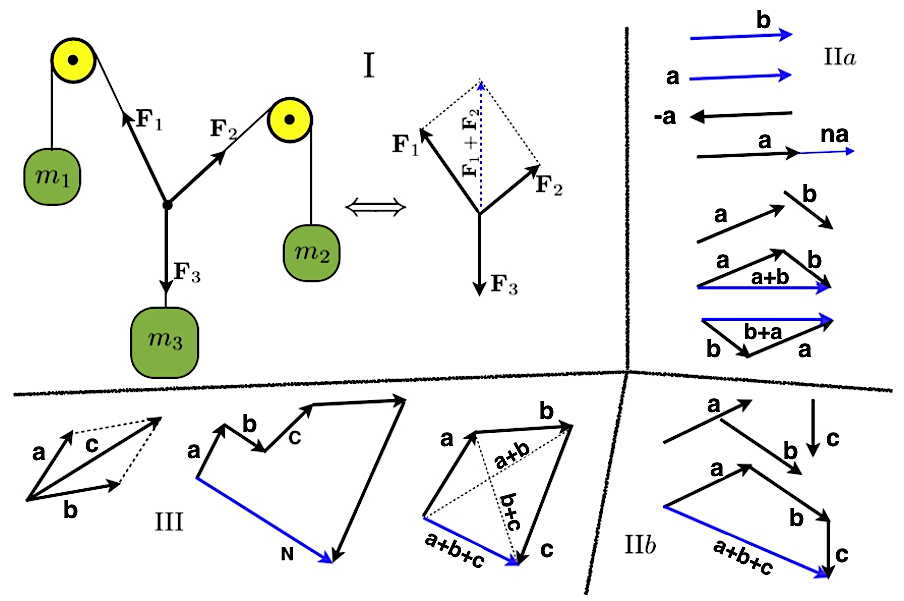
\includegraphics[height=3.1in]
{VOLUMEN_1/01_Vectores_Cartesianos/Figuras/Figura1_1.jpg}
\caption{Vectores y sus operaciones}
\label{fig1vectcartes}
\end{center}
\end{figure}

Es com�n que tropecemos con: escalares, vectores, tensores y espinores, dependiendo del n�mero de cantidades que necesitemos para representar determinado objeto matem�tico. Podremos constatar que las leyes de la F�sica vienen escritas en forma vectorial (o tensorial) y, por lo tanto, ser� la misma ley para la familia de observadores equivalentes.

\subsection{Escalares y vectores}
\label{EscalaresVectores}
\index{Vectores 3D}
Dejaremos para m�s adelante caracterizar objetos como tensores y espinores, por ahora nos contentaremos con refrescar nuestros recuerdos con cantidades como:

\begin{itemize}
\item {\textbf{Escalares: }} Ser�n aquellas cantidades las cuales se representan con UN solo n�mero, una magnitud: temperatura, volumen, masa, entre otras. Es costumbre no denotarlas de manera especial, as� $T=5^{\circ}$C representar� una temperatura de $5$ grados cent�grados.

\item{\textbf{Vectores: }} Ser�n cantidades las cuales, para ser representadas por un objeto matem�ticos, necesitan m�s de una cantidad: requieren de UN n�mero, UNA direcci�n y UN sentido. Entre las cantidades que t�picamente reconocemos como vectores est�n: la velocidad, la aceleraci�n, la fuerza. En t�rminos gr�ficos podremos decir que un vector ser� un segmento orientado, en el cual la dimensi�n del segmento representar� su m�dulo y su orientaci�n la direcci�n y el sentido. Para diferenciarlos de las cantidades escalares hay una variedad de representaciones, entre ellas: en negrita $\mathbf{a}$;  con una flecha arriba de la cantidad $\vec{a};$ con una tilde arriba o abajo $\tilde{a}$; o explicitando el origen del segmento orientado $\overrightarrow {OP}$. El m�dulo del vector lo representaremos dentro de la funci�n valor absoluto, o sencillamente sin la flecha arriba $a=\left|  \mathbf{a}\right|  =| \vec{a} | $.
\end{itemize}


%%%%%%%%%%%%%%%%%
\begin{figure}[h]
\begin{minipage}{7.8cm}
Los vectores son independientes del sistema de coordenadas. Sus caracter�sticas (m�dulo, direcci�n y sentido) se preservar�n en todos los sistemas de coordenadas. M�s a�n, habr� vectores que podremos desplazar (conservando su m�dulo direcci�n y sentido) paralelos a ellos mismos, y seguir�n representando las mismas cantidades. Por ello encontraremos el t�rmino de \textit{vectores deslizantes}. Un ejemplo son las fuerzas que act�an en un determinado cuerpo, como se muestra en el cuadrante I en la figura \ref{fig1vectcartes}. Tambi�n habr� vectores atados a un punto en el espacio, por cuanto representan una de las propiedades de ese punto: la velocidad del viento, el campo el�ctrico, o sus variaciones son ejemplos de \textit{vectores atados} (observe la figura \ref{fig2vectcartes} como ejemplos ilustrativos).
\end{minipage} \hfill 
\begin{minipage}{8.0cm} 
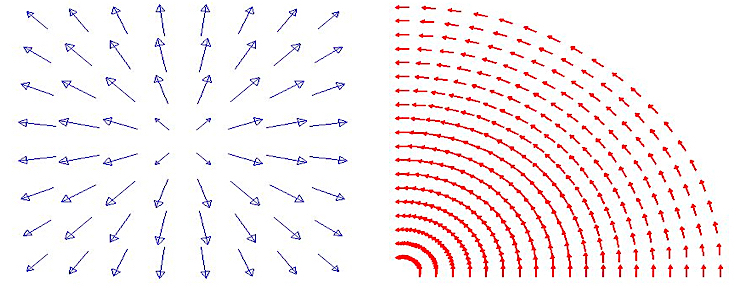
\includegraphics[height=2.0in,width=3.2in]
{VOLUMEN_1/01_Vectores_Cartesianos/Figuras/Figura1_2.jpg}
\caption{Ejemplos de \textit{vectores atados }}
\label{fig2vectcartes}
\end{minipage}
\end{figure}
%%%%%%%%%%%%%%%%%


\subsection{�lgebra de vectores}
\label{AlgebraVectores}
\index{Vectores 3D!�lgebra}
\index{�lgebra de vectores 3D}
Enumeraremos r�pidamente el �lgebra de vectores sin hacer referencia a un sistema de coordenadas en particular. Desde los cursos b�sicos de matem�ticas  nos ense�aron a representar gr�ficamente este �lgebra, as� tenemos que:

\paragraph{Vector nulo.}
Es aquel que tiene por m�dulo cero y no se le pude asignar direcci�n ni sentido. El frecuente representar al vector nulo por $\mathbf{0}$.

\paragraph{Vector unitario.}
Es aquel que tiene por m�dulo la unidad, es muy �til por cuanto, para efectos algebraicos, ``contiene'' �nicamente direcci�n y sentido. Lo denotaremos con un acento circunflejo, com�nmente llamado ``sombrero'' $\hat {\mathbf{u}}_a={\mathbf{a}}/ {| \mathbf{a} |}$,  con lo cual todo vector se podr� expresar por un m�dulo en la direcci�n y sentido de un vector unitario: $\mathbf{a}=\left| \mathbf{a}\right|  \hat{\mathbf{u}}_a =a\, \hat{\mathbf{u}}_a$.

\paragraph{Comparaci�n de vectores.}
Al comparar sus m�dulos diremos que pueden ser mayores, menores o iguales. Por lo tanto, tal y como mostramos en
el cuadrante IIa de la figura \ref{fig1vectcartes}, dos vectores ser�n iguales, $\mathbf{a}=\mathbf{b}$, si tienen la misma direcci�n y sentido. 

\paragraph{Multiplicaci�n por un n�mero.}
Un vector multiplicado por un n�mero, $\alpha$, cambiar� su m�dulo si $\alpha>0$ y cambiar� su sentido, y eventualmente
su m�dulo, si $\alpha<0$. Tal y como puede apreciarse en el cuadrante IIa de la figura \ref{fig1vectcartes}. Claramente
dos vectores proporcionales ser�n colineales. Diremos adem�s, que el inverso del vector $\mathbf{a}$ ser� la
multiplicaci�n de $\mathbf{a}$ por $\left( -1\right)$. Esto es: 
$\left( -1\right) \mathbf{a}=-\mathbf{a}$.

\paragraph{Suma de vectores.}
Para sumar vectores utilizamos la regla del paralelogramo, es decir, desplazamos paralelamente uno de los vectores y lo colocamos a continuaci�n del otro, de tal forma que la diagonal del paralelogramo, que tiene por lados los vectores sumandos, constituye el vector suma, (ver cuadrantes IIa y IIb de la figura \ref{fig1vectcartes}).

Este esquema se puede generalizar para varios vectores tal y como lo mostramos en el cuadrante III de la figura \ref{fig1vectcartes}. All� construimos un pol�gono cuyos lados los constituyen los vectores sumandos $\mathbf{a}, \mathbf{b}, \mathbf{c}$, $\mathbf{d}$ y $\mathbf{n}$ con $\mathbf{n}=\mathbf{a}+\mathbf{b}+\mathbf{c}+\mathbf{d}$. N�tese que a�n en el caso tridimensional, el vector suma siempre ser� coplanar (estar� en el mismo plano) a los sumandos que lo generaron.

Igualmente, podemos definir la resta de vectores al sumar el inverso. Esto es:
\[
\mathbf{a}-\mathbf{b}\equiv \mathbf{a}+\left(  -\mathbf{b}\right)  \quad\Rightarrow
\mathbf{0}=\mathbf{a}-\mathbf{a}\equiv\mathbf{a}+\left(  -\mathbf{a}\right) \,.
\]

En t�rminos gr�ficos la resta de dos vectores se representa colocando los vectores (minuendo y sustraendo) con el mismo origen y uniendo las cabezas de flecha. Dependiendo de cual vector es el minuendo y cual el sustraendo el vector resta apuntar� del sustraendo hacia el minuendo,  esto es:  $\left( \mathbf{a}+\mathbf{b}+\mathbf{c} \right)  -\mathbf{a}=\mathbf{b}+\mathbf{c}$.

Claramente, el m�dulo del vector resta representa la distancia entre los dos extremos de los vectores minuendo y sustraendo. 

\paragraph{Un resumen de propiedades.}

Las propiedades (obvias) del �lgebra de vectores son:
\begin{itemize}
\item  La suma de vectores:

\begin{itemize}
\item  es cerrada $\mathbf{a}+\mathbf{b}=\mathbf{c}$,

\item  es conmutativa $\mathbf{a}+\mathbf{b}=\mathbf{b}+\mathbf{a}$,

\item  es asociativa $\left(  \mathbf{a} +\mathbf{b} \right)  +\mathbf{c}=\mathbf{a}+\left(\mathbf{b}+\mathbf{c} \right)$,

\item  tiene un �nico elemento neutro $\mathbf{0}+\mathbf{a}=\mathbf{a}+\mathbf{0}=\mathbf{a}$, 
$\forall \,  \mathbf{a}$,

\item  existe un elemento sim�trico $ -\mathbf{a} $  (uno para cada vector) tal que $\mathbf{0}=\mathbf{a}-\mathbf{a} \equiv \mathbf{a}+\left(  -\mathbf{a} \right)$,

\item  es distributiva  respecto a la multiplicaci�n por n�meros: 
$\alpha\left( \mathbf{a}+\mathbf{b} \right)  =\alpha\mathbf{a}+\alpha\mathbf{b}$.
\end{itemize}

\item  La multiplicaci�n de n�meros por vectores:

\begin{itemize}
\item  es conmutativa $\mathbf{a}\alpha=\alpha\mathbf{a}$,

\item  es asociativa $\alpha\left(  \beta\mathbf{a}\right)  =\left(  \alpha\beta\right) \mathbf{a}$,

\item  es distributiva $\left(  \alpha+\beta\right) \mathbf{a}=\alpha\mathbf{a}+\beta\mathbf{a}$.
\end{itemize}
\end{itemize}


\subsection{Vectores linealmente independientes}
\label{IndependenciaVector3D}
\index{Independencia Lineal!Vectores 3D}
Armados con el �lgebra y siendo expl�cito en sus propiedades podemos construir la primera aproximaci�n a uno de los
conceptos fundamentales del �lgebra lineal. La noci�n de \textit{independencia }o \textit{dependencia lineal.} Diremos que tres vectores $\mathbf{a},\mathbf{b},\mathbf{c}$ son \textit{linealmente independientes}  en $\mathds{R}^3$ si se cumple que:
\[
\alpha\ \mathbf{a}+\beta\ \mathbf{b}+\gamma\ \mathbf{c}=\mathbf{0} \quad \Rightarrow \quad \alpha=\beta=\gamma=0 \,.
\]
Es decir, que la �nica manera que al sumar cualquier m�ltiplo de $\mathbf{a}, \mathbf{b}$ y  $\mathbf{c}$ de modo que la suma se anule es obligando a que los escalares sean \textbf{necesariamente} nulos. En caso contrario, es decir, si no se cumple lo anterior  diremos que uno de los vectores ser� \textit{linealmente dependiente} y  por lo tanto se podr� expresar como combinaci�n lineal de los otros dos. Si por ejemplo $\gamma\neq0$,  entonces: 
\[
\alpha \  \mathbf{a}+\beta \  \mathbf{b}+\gamma \ \mathbf{c}=\mathbf{0} \,\, \Rightarrow \,\, 
\mathbf{c}=-\frac{\alpha}{\gamma}\mathbf{a}-\frac{\beta}{\gamma}\mathbf{b} \,\, \Rightarrow \,\, 
\mathbf{c}=\bar{\alpha}\ \mathbf{a}+\bar{\beta}\ \mathbf{b}\,.
\]

Es muy importante se�alar que los vectores linealmente independientes formar�n una {\it base} para el espacio donde estos  vectores  ``viven'' y el n�mero m�ximo de vectores linealmente independientes ser� la dimensi�n de  ese espacio de ``residencia''. M�s adelante estudiaremos con m�s detalle el concepto de bases.

Tratemos de concretar algunas de estas afirmaciones.

\begin{itemize}
\item \textit{Dos vectores linealmente dependientes son colineales}. 
Es decir, los vectores est�n contenidos en la misma l�nea y es claro que:
\[
\alpha \ \mathbf{a}+\beta \ \mathbf{b}=\mathbf{0}\quad\text{con alguno de }\left\{
\begin{array}
[c]{c}
\alpha\neq0\\
\beta\neq0
\end{array}
\right\}  \quad  \Rightarrow \quad   \left\{
\begin{array}
[c]{c}
\mathbf{a}=-\dfrac{\beta}{\alpha}\mathbf{b}\\
\\
\mathbf{b}=-\dfrac{\alpha}{\beta}\mathbf{a}
\end{array}
\right.
\]
el contrario tambi�n ser� cierto: \textit{si dos vectores son colineales ellos ser�n linealmente dependientes.}
\[
\mathbf{a}=\lambda\mathbf{b}\,\, \Rightarrow \,\,  
\alpha\mathbf{a}+\beta\mathbf{b}=\mathbf{0}\,\, \Rightarrow \,\,  
\alpha\lambda\mathbf{b}+\beta\mathbf{b}=\mathbf{0} \,\, \Rightarrow \,\,  \left(  \alpha\lambda+\beta\right)  \mathbf{b}=\mathbf{0}\,\, \Rightarrow \,\,  
\lambda=-\frac{\beta}{\alpha} \,,
\]
con lo cual podremos afirmar que si dos vectores son linealmente independientes ellos \textbf{no} son colineales.


\item \textit{Tres vectores linealmente dependientes son coplanares}.   Por ser los tres vectores \textit{linealmente dependientes} al menos uno de los escalares tiene que ser distinto de cero, digamos  $\gamma$,  esto es:
\[
\alpha\ \mathbf{a}+\beta \ \mathbf{b}+\gamma \ \mathbf{c}= \mathbf{0}\quad  \Rightarrow \quad  
\mathbf{c}=-\frac{\alpha}{\gamma}\mathbf{a}-\frac{\beta}{\gamma}\mathbf{b}=\xi^1 \mathbf{a}+\xi^2\mathbf{b} \,,
\]
pero como $\xi^1 \mathbf{a}\propto\mathbf{a}$ y $\xi^2\ \mathbf{b}\propto \mathbf{b}$, esto significa que: $\xi^1 \mathbf{a}$ y $\mathbf{a}$  son colineales, de la misma manera que  $\xi^2 \mathbf{b}$ y  $\mathbf{b}$, y  por lo tanto, la  suma estar� en el mismo plano.

\item \textit{Dos vectores linealmente independientes generan todos los vectores coplanares}. 
Dado dos vectores $\mathbf{a}$ y $\mathbf{b}$ linealmente independientes, entonces cualquier vector
$\mathbf{c}$, coplanar con $\mathbf{a}$ y $\mathbf{b}$,  podr� expresarse como una combinaci�n lineal de �stos. Diremos que: $\mathbf{c}$ se expresa en t�rminos de $\mathbf{a}$ y $\mathbf{b}$ como: $\mathbf{c} = \xi^1\mathbf{a}+\xi^2 \mathbf{b}$, y esa expresi�n es �nica.

La primera de las afirmaciones es directa por cuanto hemos visto que si $\mathbf{a}$ y $\mathbf{b}$ son linealmente independientes y $\mathbf{c}$ es coplanar con $\mathbf{a}$ y $\mathbf{b}$, entonces, necesariamente $\mathbf{a}, \mathbf{b}$ y $\mathbf{c}$ son linealmente dependientes. Esto es:
\[
\alpha \ \mathbf{a}+\beta \ \mathbf{b}+\gamma \ \mathbf{c}={\bf 0} \,\,\Rightarrow\,\, \mathbf{c}=-\frac{\alpha}{\gamma}\mathbf{a}-\frac{\beta}{\gamma}\mathbf{b}=\xi^1 \mathbf{a}+\xi^2 \mathbf{b} \,.
\]

La demostraci�n de que la expansi�n es �nica viene de suponer que existen dos maneras distintas de representar al mismo vector $\mathbf{c}$. Veamos:
\[
\left.
\begin{array}
[c]{c}
\mathbf{c}=\xi^1 \mathbf{a}+\xi^2 \mathbf{b}\\
\\
\mathbf{c}=\zeta^1 \mathbf{a}+\zeta^2 \mathbf{b}
\end{array}
\right\}  \,\,\Rightarrow\,\, \mathbf{0}=\left( \xi^1-\zeta^1\right)   \mathbf{a}+
\left( \xi^2-\zeta^2\right)   \mathbf{b}\,\,\Rightarrow\,\,\left\{
\begin{array}
[c]{c}
 \xi^1-\zeta^1 =0\,\,\Rightarrow\,\, \quad \xi^1=\zeta^1\\
\\
\xi^2-\zeta^2=0\,\,\Rightarrow\,\, \quad \xi^2=\zeta^2
\end{array}
\right.
\]
debido a que $\mathbf{a}$ y $\mathbf{b}$ son linealmente independientes. 

La demostraci�n para el caso tridimensional es equivalente. Es decir tres vectores linealmente independientes $\mathbf{a},\mathbf{b}$ y $\mathbf{c}$ expanden, de manera un�voca, todos los vectores del espacio. Esta demostraci�n queda para el lector.

\item \textit{Vectores Base}.   Cuando un vector $\mathbf{c}$ se pueda expresar en t�rminos de dos vectores linealmente independientes, $\mathbf{a}$ y $\mathbf{b}$, por ejemplo: $\mathbf{c}=\xi^1\mathbf{a}+\xi^2\mathbf{b}$, diremos que $\mathbf{a}$ y $\mathbf{b}$ forman una base para todos los vectores coplanares a �stos. Igualmente para el caso tridimensional: tres vectores linealmente independientes $\mathbf{a},\mathbf{b}$ y $\mathbf{c}$ conformar�n una base para los vectores del espacio. Los n�meros $\xi^1$ y $\xi^2$ para el caso bidimensional se denominan las componentes de $\mathbf{c}$ a lo largo de $\mathbf{a}$ y $\mathbf{b}$. Equivalentemente, $\left(\xi^1, \xi^2, \xi^3\right)$ ser�n las componentes de cualquier vector para el caso 3D a lo largo de $\mathbf{a},\mathbf{b}$ y $\mathbf{c},$ respectivamente. Esta nomenclatura ser� m�s evidente luego de la pr�xima secci�n.
\end{itemize} 

\begin{figure}[t]
\begin{center}
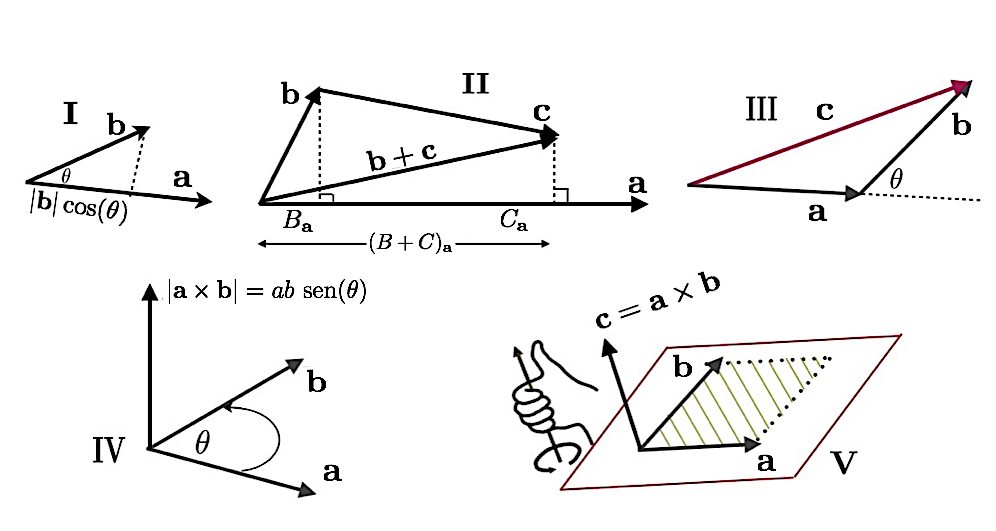
\includegraphics[height=3.0in,width=5.8in]
{VOLUMEN_1/01_Vectores_Cartesianos/Figuras/Figura1_3.jpg}
\caption{Productos de vectores}
\label{fig3vectcartes}
\end{center}
\end{figure}

\subsection{Productos de vectores}
\label{ProductosVectores}
\index{Productos de Vectores 3D}
\index{Vectores 3D!Productos}
\index{Producto!Vectores 3D}

Hemos sumado y restado vectores, el siguiente paso es multiplicarlos. B�sicamente existen dos formas de multiplicar vectores: el producto  escalar y el producto vectorial, veremos a continuaci�n de que se trata y sin especificar un sistema de coordenadas para referirlos. 

\subsubsection{Producto escalar}
\label{ProductoEscalar1}
\index{Producto escalar}
\index{Producto!escalar}
\index{Escalar!Producto}
\index{Desigualdad de Cauchy-Schwarz!Vectores 3D}
Denominaremos producto escalar de dos vectores $\mathbf{a}$ y $\mathbf{b}$ a un escalar cuyo valor ser� igual al
producto de los m�dulos multiplicado por el coseno del �ngulo que ellos forman:
\[
\zeta=\mathbf{a}\cdot\mathbf{b}=\left|  \mathbf{a}\right|  \left|  \mathbf{b}\right|
\cos(\theta)_{\left\langle \mathbf{a},\mathbf{b}\right\rangle } \,.
\]

El significado geom�trico del producto escalar es evidente, cuadrante I de la figura \ref{fig3vectcartes}. El producto escalar representa la proyecci�n de $\mathbf{a}$ sobre $\mathbf{b}$ y equivalentemente la proyecci�n de $\mathbf{b}$ sobre $\mathbf{a}$.

De esta definici�n se derivan varias consecuencias las cuales por obvias no dejan de ser importantes:
\begin{itemize}
\item \textit{El producto escalar de un vector consigo mismo, siempre es positivo}:\\
 $\zeta=\mathbf{a}\cdot\mathbf{a}=\left|  \mathbf{a}\right| ^{2}\geq0$, y s�lo ser� nulo si $\mathbf{a}$
es el vector nulo. Esto es, $\zeta=0 \,\,  \Rightarrow \,\,  \mathbf{a}=\mathbf{0}$. Con esto podemos concluir que $\left|\mathbf{a}\right|  =\sqrt{\mathbf{a}\cdot\mathbf{a}}=\sqrt{\zeta}$.

\item \textit{El producto escalar es conmutativo}:\\
$\zeta=\mathbf{a}\cdot\mathbf{b}=\mathbf{b}\cdot\mathbf{a}$,  ya que el �ngulo entre los vectores es el mismo y la multiplicaci�n entre escalares es conmutativa.

\item \textit{El producto escalar es distributivo}: \\
Esto es, $\mathbf{a} \cdot\left(  \mathbf{b}+\mathbf{c}\right)  =\mathbf{a}\cdot\mathbf{b} +\mathbf{a}\cdot\mathbf{c}$. La demostraci�n (gr�fica) puede apreciarse en el cuadrante II de la figura \ref{fig3vectcartes}.

\item \textit{La multiplicaci�n por un n�mero}:\\$
\bar{\zeta}=\alpha \zeta  = \left|  \alpha\right|  \left(  \mathbf{a}\cdot\mathbf{b}\right)  =
\left(\alpha\mathbf{a}\right)  \cdot\mathbf{b}=\mathbf{a} \cdot \left(  \alpha\mathbf{b}\right)=
\left|  \alpha\mathbf{a}\right|  \left|  \mathbf{b}\right|  \cos(\theta)_{\left\langle \mathbf{a},\mathbf{b}\right\rangle }=
\left|  \mathbf{a}\right|  \left| \alpha\mathbf{b}\right|  \cos(\theta)_{\left\langle \mathbf{a},\mathbf{b}\right\rangle }$.

\item \textit{Desigualdad de Cauchy-Schwarz}. \\
A partir de la definici�n de producto interno es inmediata la comprobaci�n de la siguiente desigualdad:
\[
\left(  \mathbf{a}\cdot\mathbf{b}\right)^{2}=\left(  \left|  \mathbf{a}\right|
\left|  \mathbf{b}\right|  \cos(\theta)_{\left\langle \mathbf{a},\mathbf{b}\right\rangle}\right) ^{2}\,\,  \Rightarrow \,\,  \left(  \mathbf{a}\cdot\mathbf{b}\right)^{2}
\leq\left|  \mathbf{a}\right|  ^{2}\left|  \mathbf{b}\right| ^{2}
\,\, \Leftrightarrow \,\,  \mathbf{a}\cdot\mathbf{b}  \leq\left|  \mathbf{a}\right|  \left|  \mathbf{b}\right| \,,
\]
ya que: $0\leq\cos^{2}(\theta)_{\left\langle \mathbf{a},\mathbf{b}\right\rangle }\leq1$.

\item \textit{Del producto escalar surge el teorema del coseno}.\\
Es inmediato calcular el producto escalar de un vector consigo mismo, para ello vamos a suponer que $\mathbf{c}=\mathbf{a}+\mathbf{b}$, con lo cual:
\[
\mathbf{c}=\mathbf{a}+\mathbf{b}\,\,  \Rightarrow \,\,  \mathbf{c}\cdot\mathbf{c}=\left(  \mathbf{a}+\mathbf{b}\right)  \cdot\left(  \mathbf{a}+\mathbf{b}\right)  \,\,  \Rightarrow \,\, 
\left|  \mathbf{c} \right|^{2}=\left|  \mathbf{a}\right|^{2}+\left|  \mathbf{b}\right|^{2} + 2\left|  \mathbf{a}\right|  \left|  \mathbf{b}\right| \cos(\theta)\,,
\]
donde $\theta$ es el �ngulo que forman los vectores $\mathbf{a}$ y $\mathbf{b}$. Esto no  es otra cosa que el teorema del coseno y est� ilustrado en el cuadrante III de la figura \ref{fig3vectcartes}.

\item \textit{Dos vectores no nulos son ortogonales (perpendiculares) si su producto escalar es nulo}.\\
 Esta afirmaci�n es inmediata:
\[
\mathbf{a}\ \bot\ \mathbf{b} \,\,\Rightarrow\,\,  \theta_{\left\langle \mathbf{a},\mathbf{b}\right\rangle }=
\frac{\pi}{2} \,\,\Rightarrow\,\,  \mathbf{a}\cdot\mathbf{b}=\left|
\mathbf{a}\right|  \left|  \mathbf{b}\right|  \cos(\theta)_{\left\langle \mathbf{a} ,\mathbf{b}\right\rangle }=0\,.
\]
\end{itemize}


\subsubsection{Producto vectorial} 
\label{ProductorVectorial1} 
\index{Producto vectorial}
A diferencia del producto escalar que genera un escalar, el producto vectorial tiene como resultado otro vector: $\mathbf{c}=\mathbf{a}\times\mathbf{b}$  (realmente un pseudovector o vector axial en contraposici�n a los vectores polares, pero eso lo veremos m�s adelante en la secci�n \ref{PseudoCantidades}), con las siguientes caracter�sticas:

\begin{itemize}
\item  El m�dulo de $\mathbf{c}$, ser�:
\[
\left|  \mathbf{c}\right|  =\left|
\mathbf{a}\right|  \left|  \mathbf{b}\right|  \operatorname*{sen}(\theta)_{\left\langle \mathbf{a},\mathbf{b}\right\rangle}\,.
\] 
Es claro que el m�dulo de $\mathbf{c}$ representa el �rea del paralelogramo cuyos lados est�n formados por $\mathbf{a}$ y $\mathbf{b}$ (ver el cuadrante V de la figura \ref{fig3vectcartes}).

\item  Tal y como muestran los cuadrantes IV y V de la figura
\ref{fig3vectcartes}, $\mathbf{c}$ tendr� como direcci�n la perpendicular al plano que forman $\mathbf{a}$ y $\mathbf{b}$, y como sentido la regla del pulgar derecho, regla de la mano derecha, o de manera  m�s elegante, ser� positiva cuando la multiplicaci�n de $\mathbf{a} \times\mathbf{b}$ corresponda  al sentido antihorario.
\end{itemize}

Podemos deducir algunas consecuencias de esta definici�n.
\begin{itemize}
\item \textit{El producto vectorial es anticonmutativo}.\\
$\mathbf{a}\times\mathbf{b}=-\mathbf{b}\times\mathbf{a}$, y se sigue de la definici�n que expresa el cuadrante IV de la figura \ref{fig3vectcartes}.

\item \textit{El producto vectorial es distributivo respecto a la suma}.\\
$\mathbf{a}\times\left(  \mathbf{b}+\mathbf{c}\right)  =\mathbf{a} \times  \mathbf{b} +\mathbf{a}\times\mathbf{c}$. La demostraci�n de esto lo dejaremos para m�s adelante. 
\item \textit{La multiplicaci�n por un n�mero}.
\[
\left|  \mathbf{c}\right|  =\left|  \alpha\right|  \left|  \mathbf{a}\times\mathbf{b} \right|  =
\left|  \left(  \alpha\mathbf{a}\right)  \times\mathbf{b}\right|=\left|  \mathbf{a}\times\left(  \alpha\mathbf{b}\right) \right|  = 
\left| \alpha\mathbf{a}\right|  \left|  \mathbf{b}\right|  \operatorname{sen}(\theta)_{\left\langle \mathbf{a},\mathbf{b}\right\rangle}=
\left|  \mathbf{a}\right|  \left|  \alpha\mathbf{b}\right|  \operatorname{sen}(\theta)_{\left\langle \mathbf{a},\mathbf{b}\right\rangle}\,.
\]

\item \textit{Dos vectores ser�n colineales si su producto vectorial se anula}. \\
Como en el caso cuando se anulaba el producto escalar 
identific�bamos a dos vectores ortogonales, cuando se anula el producto vectorial tendremos dos vectores paralelos. Es claro que esto se cumple de inmediato:
\[
\mathbf{a}\ \Vert\ \mathbf{b}\,\,\Rightarrow\,\,  
\theta_{\left\langle \mathbf{a},\mathbf{b}\right\rangle}=0
\,\,\Rightarrow\,\,  \left|  \mathbf{c}\right|  =\left|  \mathbf{a}\times\mathbf{b}\right|
=\left|  \mathbf{a}\right|  \left|  \mathbf{b}\right|  \operatorname{sen}(\theta)_{\left\langle \mathbf{a},\mathbf{b}\right\rangle}=0\,.
\]

Si el m�dulo del vector es cero, obvio que es el vector nulo. Ahora bien, tambi�n de aqu� deducimos que:
\[
\mathbf{c}=\mathbf{a}\times\mathbf{b} \,\,\Rightarrow\,\,  \mathbf{c}\cdot\mathbf{a}=\left(\mathbf{a}\times\mathbf{b}\right)  \cdot\mathbf{a}=\mathbf{c}\cdot\mathbf{b}=\left(  \mathbf{a}\times\mathbf{b}\right)  \cdot\mathbf{b}=0\,.
\]
\end{itemize}

\subsection{Producto triple o mixto}
\label{ProductoTriple}
\index{Producto Triple}
\index{Producto Mixto}
Analicemos ahora el n�mero (pseudoescalar) que proviene de la multiplicaci�n:
\[
V=\mathbf{c}\cdot\left(  \mathbf{a}\times\mathbf{b}\right)  =\left|  \mathbf{c}\right|
\left|  \left(  \mathbf{a}\times\mathbf{b}\right)  \right|  \cos(\theta)_{\left\langle
\mathbf{c},\mathbf{a}\times\mathbf{b}\right\rangle }\,.
\]
Este producto tambi�n cumple con algunas propiedades que enunciaremos ahora y demostraremos m�s tarde.

\begin{itemize}
\item \textit{El producto mixto representa el volumen del paralelep�pedo cuyos lados son los vectores }$\mathbf{a},\mathbf{b}$ y $\mathbf{c}$. \\
 $\left|  \mathbf{a}\times \mathbf{b}  \right| $ representa el �rea de la base y la altura est� representada por la proyecci�n del vector $\mathbf{c}$ sobre la perpendicular al plano de la base que es, precisamente $\left| \mathbf{c}\right|  \cos
(\theta)_{\left\langle \mathbf{c},\mathbf{a}\times\mathbf{b}\right\rangle }$.
\item \textit{El producto mixto es c�clico respecto a sus factores}.
\[
\left(  \mathbf{a}\times\mathbf{b}\right)  \cdot\mathbf{c}=
\left(  \mathbf{c}\times\mathbf{a}\right)  \cdot\mathbf{b}=
\left(  \mathbf{b}\times\mathbf{c}\right)  \cdot\mathbf{a} \,.
\]
Esta afirmaci�n se ver� demostrada m�s adelante.
\item \textit{El producto mixto se anula cuando se repite alguno de sus factores}.
\[
\left(  \mathbf{a}\times\mathbf{b}\right)  \cdot \mathbf{a}=
  \left(  \mathbf{a} \times \mathbf{b}\right)  \cdot \mathbf{b}=
  \left(  \mathbf{a}\times\mathbf{a}\right) \cdot\mathbf{c}=
  \left(  \mathbf{b}\times\mathbf{b}\right)  \cdot \mathbf{c}=0\,.
\]
Claramente, si $\left( \mathbf{a}\times\mathbf{b}\right)  \bot \, \mathbf{a} \,\,\Rightarrow\,\, 
\left(  \mathbf{a}\times\mathbf{b}\right)  \cdot\mathbf{a}=0$.

\item \textit{Si los tres vectores }$\mathbf{a},\mathbf{b}$\textit{ y }$ \mathbf{c} 
$\textit{ son coplanares (linealmente dependientes) entonces:} 
\[
\left( \mathbf{a}\times\mathbf{b}\right)\cdot\mathbf{c}=0 \,. 
\] 
Dicho de manera m�s elegante, �til e impactante: tres vectores que cumplen con:
\[
\left(\mathbf{a}\times\mathbf{b}\right)  \cdot\mathbf{c}\neq0 \,,
\]
son linealmente independientes y forman una base para el espacio tridimensional. 
Esa base se denominar� lev�gira (contraria al giro de las manecillas del reloj) si el producto 
$\left( \mathbf{a}\times\mathbf{b}\right) \cdot \mathbf{c}<0$ y dextr�gira (la convencional base de la 
mano derecha) si $\left( \mathbf{a}\times\mathbf{b}\right) \cdot\mathbf{c}>0.$
\end{itemize}

\subsection{{\color{Fuchsia}Ejemplos}}
\label{EjemploVectores}
\begin{enumerate}

\item En un segmento de recta $AB$ ubicamos un punto $D$ de manera que este punto divide al segmento en dos partes, es decir, en la proporci�n $\alpha$ : $\beta$ $(\overline{AB}=\overline{AD}+\overline{DB}=\alpha+\beta)$. Para ubicar el vector posici�n del punto $D$ podemos hacer lo siguiente.

A los puntos $A$ y $B$ le hacemos corresponder el vector ${\bf a}$ y el vector ${\bf b}$, respectivamente, con un origen com�n $O$. De manera que ${\bf c}={\bf b}-{\bf a}$  es un vector que va desde el punto $A$ al punto $B$. Entonces, la distancia $\overline{OD}$, a la que le podemos asociar  el vector ${\bf d}$,  no es m�s que:
\[
{\bf d}= \overline{OD}= 
{\bf a}+\frac{\alpha}{\alpha+\beta}({\bf b}-{\bf a}) =
\left(1- \frac{\alpha}{\alpha+\beta} \right){\bf a} + 
\frac{\alpha}{\alpha+\beta}{\bf b}= 
\frac{\beta}{\alpha+\beta}{\bf a} + \frac{\alpha}{\alpha+\beta}{\bf b}\,.
\]


\item Hemos definido la posici�n ${\bf r}$ del  centro de masa, para un sistema de $N$ part�culas, al vector:
\[
{\bf r} = \frac{\Sigma_{i=1}^{N} m_{i} {\bf r}_{i} }{\Sigma_{j=1}^{N} m_{j}}\,,
\]
donde ${\bf r}_{i}$ corresponde con la posici�n de la $i-$�sima part�cula.
Determinaremos la posici�n del centro de masa para un sistema de tres masas, $m_{i} =$ 1,2,3, ubicadas en los v�rtices de un tri�ngulo equil�tero de lado $l=2$.

Colocando el origen de coordenadas en uno de los v�rtices y uno de los ejes de coordenadas sobre uno de los lados, entonces tenemos:
\[
{\bf r} = \frac{\Sigma_{i=1}^{3} m_{i} {\bf r}_{i} }{\Sigma_{j=1}^{3} m_{j}} = \frac{m_{1}{\bf r}_{1} +  m_{1}{\bf r}_{1} }{M_{T}} = \frac{1 \cdot 2 {\bf i} + 3 \cdot \left({\bf i} + \sqrt{3} {\bf j}  \right)}{6} =  \frac{ 5}{6 }{\bf i} + \frac{\sqrt{3}}{2} {\bf j} \,.
\]


\item Dada una base ortonormal $\{ {\bf i}, {\bf j}, {\bf k} \}$ y los siguientes vectores:
\[
{\bf a} = 3{\bf i} + 2{\bf j} + {\bf k}\,, \quad {\bf b} = 3{\bf i} - 2{\bf j} + {\bf k}\,, \quad {\bf c} = {\bf i} -  {\bf k} \,.
\]

Queremos comprobar si $\{ {\bf a}, {\bf b}, {\bf c} \}$ forman una base.
  
Veamos, para que los vectores formen una base tienen que ser linealmente independientes. Esto es:
$
\alpha {\bf a} + \beta {\bf b} + \gamma  {\bf c}  =0 \,\, \Rightarrow \,\, \alpha = \beta = 
\gamma = 0 $,  con lo cual:
\[
\alpha \left(  3{\bf i} + 2{\bf j} + {\bf k} \right) + \beta \left(  3{\bf i} - 2{\bf j} + {\bf k} \right) + 
\gamma  \left(  {\bf i} -  {\bf k}  \right) =0 \,\, \Rightarrow \,\, 
\left\{\begin{array}{ l}
  3 \alpha + 3 \beta + \gamma = 0      \\
  2 \alpha - 2 \beta  = 0        \\
   \alpha +  \beta - \gamma = 0          
\end{array} 
\right.
\]
es f�cil ver que la soluci�n de este sistema es: $\alpha = \beta = \gamma =0$, por lo tanto, se demuestra que los vectores son linealmente independientes y por consiguiente forman una base.

Otra manera de resolverlo es mostrar que: ${\bf c} \cdot \left( {\bf a} \times {\bf b} \right) \neq 0$, y efectivamente:
\[
{\bf c} \cdot \left( {\bf a} \times {\bf b} \right) = \left|\begin{array}{ccc}1 & 0 & -1 \\3 & 2 & 1 \\3 & -2 & 1\end{array}\right| = 4 \neq 0 \,.
\]

Ahora bien,  si $\{ {\bf a}, {\bf b}, {\bf c} \}$ forman una base, podemos expresar otros vectores en t�rminos de �sta base. Tomemos los vectores: ${\bf d} = {\bf i} + 2{\bf j}\,, \,\, {\bf e} = 3{\bf i} - 2{\bf j}$ y ${\bf f} = {\bf a} \times {\bf b}$ y expres�moslos en t�rminos de $\{ {\bf a}, {\bf b}, {\bf c} \}$. 
  
Entonces, para el vector {\bf d} tenemos:
 \[
{\bf d}= {\bf i} + 2{\bf j} = \alpha \left(  3{\bf i} + 2{\bf j} + {\bf k}\right) + \beta \left(  3{\bf i} - 2{\bf j} + {\bf k}\right) + \gamma  \left(  {\bf i} -  {\bf k} \right)  \,\, \Rightarrow \,\, 
\left\{\begin{array}{ l}
  3 \alpha + 3 \beta + \gamma = 1      \\
  2 \alpha - 2 \beta  = 2        \\
   \alpha +  \beta - \gamma = 0          
\end{array} 
\right.
\] 
resolviendo el sistema de ecuaciones anterior tendremos que: ${\bf d} = \frac{5}{8} {\bf a} -\frac{3}{8}  {\bf b} + \frac{1}{4} {\bf c}$. 

Seguidamente, para el vector {\bf e} se tiene: 
 \[
{\bf e}=3{\bf i} - 2{\bf j} = \alpha \left(  3{\bf i} + 2{\bf j} + {\bf k}\right) + \beta \left(  3{\bf i} - 2{\bf j} + {\bf k}\right) + \gamma  \left(  {\bf i} -  {\bf k} \right)  \,\, \Rightarrow \,\, 
\left\{\begin{array}{ l}
  3 \alpha + 3 \beta + \gamma = 3      \\
  2 \alpha - 2 \beta  = -2        \\
   \alpha +  \beta - \gamma = 0          
\end{array} 
\right.
\] 
resolviendo el nuevo sistema de ecuaciones resulta que: ${\bf e} = -\frac{1}{8} {\bf a} +\frac{7}{8}  {\bf b} + \frac{3}{4}   {\bf c} $.

Ahora bien, 
\[
{\bf f}= {\bf a} \times {\bf b}= \left(  3{\bf i} + 2{\bf j} + {\bf k}\right) \times  \left(  3{\bf i} - 2{\bf j} + {\bf k}\right)= \left|\begin{array}{ccc}{\bf i} & {\bf j} & {\bf k}\\3 & 2 & 1 \\3 & -2 & 1\end{array}\right| =
 4{\bf i}  -12{\bf k}\,,
\]
con lo cual para el vector {\bf f} resulta:
 \[
{\bf f}=4{\bf i}  -12{\bf k}= \alpha \left(  3{\bf i} + 2{\bf j} + {\bf k}\right) + \beta \left(  3{\bf i} - 2{\bf j} + {\bf k}\right) + \gamma  \left(  {\bf i} -  {\bf k} \right)  \,\, \Rightarrow \,\, 
\left\{\begin{array}{ l}
  3 \alpha + 3 \beta + \gamma = 4      \\
  2 \alpha - 2 \beta  = 0        \\
   \alpha +  \beta - \gamma = -12          
\end{array} 
\right.
\]
y finalmente, al resolver el sistema anterior,  ${\bf f}=  {\bf a} \times {\bf b} = -{\bf a} - {\bf b} +10   {\bf c}$\,.


\item  Consideremos los siguientes tres vectores: ${\bf w}_{1}={\bf i} +3 {{\bf k}}\,,  {\bf w}_{2}
=2{\bf i}-3{\bf j}$ y ${\bf w}_{3}=-{\bf j}+ {\bf k}$ �Formar�n una base para $\mathds{R}^{3}$? 

Veamos entonces si son linealmente independientes:
\[\alpha {\bf w}_{1} + \beta{\bf w}_{2} +\gamma {\bf w}_{3} = 0 \,\, \Rightarrow \,\, \alpha=\beta=\gamma= 0 \,,
\]
La comprobaci�n es directa al resolver el siguiente sistema de ecuaciones:
\[
\left.
\begin{array}{cccc}
\alpha & +2 \beta &  & =0 \\ 
& -3 \beta & - \gamma & =0 \\
3 \alpha &  & +\gamma & =0 
\end{array}\right.
\]
cuya soluci�n es $\alpha=\beta=\gamma= 0$. Por lo tanto, forman una base para $\mathds{R} ^{3}$.

Como forman base, podemos expresar otro vector, digamos: ${\bf a}={\bf i} -3{\bf j}+3{\bf k}$, en t�rmino de la base $\left\{ {\bf w}_{1}, {\bf w}_{2}, {\bf w}_{3}\right\} $, esto es:
\[
{\bf a} = \alpha {\bf w}_{1} + \beta {\bf w}_{2} +\gamma {\bf w}_{3} \,\, \Rightarrow \,\, 
\left\{
\begin{array}{cccc}
\alpha & +2 \beta &  & =1 \\
 & -3 \beta & - \gamma & =-3 \\
 3 \alpha &  & +\gamma & =3
\end{array}\right\} \,\, \Rightarrow \,\,\left\{ 
\begin{array}{c}\alpha = \frac{1}{3} \\ \\ \beta = \frac{1}{3} \\ \\ \gamma = 2 \end{array} \right.
\]
es decir:
\[
{\bf a} = \frac{1}{3} {\bf w}_{1} + \frac{1}{3} {\bf w}_{2} +2 {\bf w}_{3}\,.
\]
\end{enumerate}

\newpage
\subsection{{\color{red}Practicando con Maxima}} 

El programa de manipulaci�n simb�lica {\bf Maxima} est� dise�ado para realizar una gran cantidad de c�lculos algebraicos y num�ricos que iremos descubriendo a medida que desarrollemos los diferentes temas de este curso. Es indispensable ir al ap�ndice \ref{IntroMaxima} para familiarizarnos con la sintaxis b�sica del programa. 

{\bf Maxima} es una potente calculadora y maneja n�meros de diferentes tipos: enteros, racionales, irracionales, complejos y n�meros con decimales (punto flotante). 

Haremos algunos c�lculos sencillos para ir calentando. 

%%%%%% INPUT:
\begin{minipage}[t]{8ex}
{\color{red}\bf \begin{verbatim} (%i1) 
\end{verbatim}}
\end{minipage}
\begin{minipage}[t]{\textwidth}{\color{blue}
\begin{verbatim}
log(20);
\end{verbatim}}
\end{minipage}

%%% OUTPUT:
\begin{math}\displaystyle \parbox{8ex}{\color{labelcolor}(\%o1) }
\log(20)
\end{math}
\newline

Es probable que necesitemos el valor num�rico de $\log(20)$.

%%%%%% INPUT:
\begin{minipage}[t]{8ex}
{\color{red}\bf \begin{verbatim} (%i2) 
\end{verbatim}}
\end{minipage}
\begin{minipage}[t]{\textwidth}{\color{blue}
\begin{verbatim}
log(20),numer;
\end{verbatim}}
\end{minipage}

%%% OUTPUT:
\begin{math}\displaystyle \parbox{8ex}{\color{labelcolor}(\%o2) }
2.995732273553991
\end{math}


%%%%%% INPUT:
\begin{minipage}[t]{8ex}
{\color{red}\bf \begin{verbatim} (%i3) 
\end{verbatim}}
\end{minipage}
\begin{minipage}[t]{\textwidth}{\color{blue}
\begin{verbatim}
420/16000;
\end{verbatim}}
\end{minipage}

%%% OUTPUT:
\begin{math}\displaystyle \parbox{8ex}{\color{labelcolor}(\%o3) }
\frac{21}{800}
\end{math}

%%%%%% INPUT:
\begin{minipage}[t]{8ex}
{\color{red}\bf \begin{verbatim} (%i4) 
\end{verbatim}}
\end{minipage}
\begin{minipage}[t]{\textwidth}{\color{blue}
\begin{verbatim}
420/16000,numer;
\end{verbatim}}
\end{minipage}

%%% OUTPUT:
\begin{math}\displaystyle \parbox{8ex}{\color{labelcolor}(\%o4) }
0.02625
\end{math}
\newline

Podemos utilizar la funci�n {\bf float} para el mismo resultado

%%%%%% INPUT:
\begin{minipage}[t]{8ex}
{\color{red}\bf \begin{verbatim} (%i5) 
\end{verbatim}}
\end{minipage}
\begin{minipage}[t]{\textwidth}{\color{blue}
\begin{verbatim}
float(log(20)); float(420/16000);
\end{verbatim}}
\end{minipage}

%%% OUTPUT:
\begin{math}\displaystyle \parbox{8ex}{\color{labelcolor}(\%o5) }
2.995732273553991
\end{math}

%%% OUTPUT:
\begin{math}\displaystyle \parbox{8ex}{\color{labelcolor}(\%o6) }
0.02625
\end{math}
\newline

El programa contiene una gran cantidad de funciones matem�ticas b�sicas internas y entre ellas las trigonom�tricas:

%%%%%% INPUT:
\begin{minipage}[t]{8ex}
{\color{red}\bf \begin{verbatim} (%i7) 
\end{verbatim}}
\end{minipage}
\begin{minipage}[t]{\textwidth}{\color{blue}
\begin{verbatim}
sin(%pi/3);cos(%pi/3);tan(%pi/3);
\end{verbatim}}
\end{minipage}

%%% OUTPUT:
\begin{math}\displaystyle \parbox{8ex}{\color{labelcolor}(\%o7) }
\frac{\sqrt{3}}{2}
\end{math}

%%% OUTPUT:
\begin{math}\displaystyle \parbox{8ex}{\color{labelcolor}(\%o8) }
\frac{1}{2}
\end{math}

%%% OUTPUT:
\begin{math}\displaystyle \parbox{8ex}{\color{labelcolor}(\%o9) }
\sqrt{3}
\end{math}
\newline 

Ahora recurriremos a una de las facilidades que nos ofrece el programa para agrupar objetos matem�ticos: las listas. Las listas se escriben entre corchetes y los objetos de la lista separados con comas. 

%%%%%% INPUT:
\begin{minipage}[t]{8ex}
{\color{red}\bf \begin{verbatim} (%i10) 
\end{verbatim}}
\end{minipage}
\begin{minipage}[t]{\textwidth}{\color{blue}
\begin{verbatim}
[sin(%pi/3),cos(%pi/3),tan(%pi/3)];
\end{verbatim}}
\end{minipage}

%%% OUTPUT:
\begin{math}\displaystyle \parbox{8ex}{\color{labelcolor}(\%o10) }
\left[ \frac{\sqrt{3}}{2} , \frac{1}{2} , \sqrt{3} \right] 
\end{math}

%%%%%% INPUT:
\begin{minipage}[t]{8ex}
{\color{red}\bf \begin{verbatim} (%i11) 
\end{verbatim}}
\end{minipage}
\begin{minipage}[t]{\textwidth}{\color{blue}
\begin{verbatim}
[sin(%pi/3),cos(%pi/3),tan(%pi/3)],numer;
\end{verbatim}}
\end{minipage}

%%% OUTPUT:
\begin{math}\displaystyle \parbox{8ex}{\color{labelcolor}(\%o11) }
\left[ 0.8660254037844386 , 0.5000000000000001 , 1.732050807568877  \right] 
\end{math}
\newline

Cuando necesitemos generar una lista por medio de alguna regla espec�fica o formula usamos la funci�n {\bf makelist}. La sintaxis es la siguiente:

%%%%%% INPUT:
\begin{minipage}[t]{8ex}
{\color{red}\bf \begin{verbatim} (%i12) 
\end{verbatim}}
\end{minipage}
\begin{minipage}[t]{\textwidth}{\color{blue}
\begin{verbatim}
makelist(exp(t*x),t,1,10);
\end{verbatim}}
\end{minipage}

%%% OUTPUT:
\begin{math}\displaystyle \parbox{8ex}{\color{labelcolor}(\%o12) }
\left[ e^{x} , e^{2\,x} , e^{3\,x} , e^{4\,x} , e^{5\,x} , e^{6\,x}
  , e^{7\,x} , e^{8\,x} , e^{9\,x} , e^{10\,x} \right] 
\end{math}
\newline

Podemos tambi�n aplicar una funci�n a cada elemento de la lista, en este caso a cada elemento le aplicaremos la funci�n $\ln(x)$. Para tal fin utilizaremos el comando {\bf map}.

%%%%%% INPUT:
\begin{minipage}[t]{8ex}
{\color{red}\bf \begin{verbatim} (%i13) 
\end{verbatim}}
\end{minipage}
\begin{minipage}[t]{\textwidth}{\color{blue}
\begin{verbatim}
map(log,(makelist(exp(t*x),t,1,10)));
\end{verbatim}}
\end{minipage}

%%% OUTPUT:
\begin{math}\displaystyle \parbox{8ex}{\color{labelcolor}(\%o13) }
\left[ x , 2\,x , 3\,x , 4\,x , 5\,x , 6\,x , 7\,x , 8\,x , 9\,x , 
 10\,x \right] 
\end{math}
\newline

Si queremos, por ejemplo, sumar todos los elementos de la lista anterior utilizamos la funci�n {\bf apply} con la operaci�n que queremos realizar. Aqu� aprovecharemos para utilizar un atajo muy pr�ctico que consiste en el uso del s�mbolo $\%$, que toma la �ltima salida del programa para ser usado en la instrucci�n siguiente, de esta manera nos evitamos volver a escribir toda la instrucci�n anterior. La sintaxis para todo esto es:

%%%%%% INPUT:
\begin{minipage}[t]{8ex}
{\color{red}\bf \begin{verbatim} (%i14) 
\end{verbatim}}
\end{minipage}
\begin{minipage}[t]{\textwidth}{\color{blue}
\begin{verbatim}
apply("+",%);
\end{verbatim}}
\end{minipage}

%%% OUTPUT:
\begin{math}\displaystyle \parbox{8ex}{\color{labelcolor}(\%o14) }
55\,x
\end{math}
\newline

Podemos asignarle a una lista el nombre de una variable.

%%%%%% INPUT:
\begin{minipage}[t]{8ex}
{\color{red}\bf \begin{verbatim} (%i15) 
\end{verbatim}}
\end{minipage}
\begin{minipage}[t]{\textwidth}{\color{blue}
\begin{verbatim}
L:[sin(%pi/3),log(3),sqrt(2),abs(x),exp(x^2)];
\end{verbatim}}
\end{minipage}

%%% OUTPUT:
\begin{math}\displaystyle \parbox{8ex}{\color{labelcolor}(\%o15) }
\left[ \frac{\sqrt{3}}{2} , \log(3) , \sqrt{2} , \left| x\right|  , 
 e^{x^2} \right] 
\end{math}
\newline

De manera que para aislar  elementos de una lista escribimos:

%%%%%% INPUT:
\begin{minipage}[t]{8ex}
{\color{red}\bf \begin{verbatim} (%i16) 
\end{verbatim}}
\end{minipage}
\begin{minipage}[t]{\textwidth}{\color{blue}
\begin{verbatim}
L[1]; L[4];
\end{verbatim}}
\end{minipage}

%%% OUTPUT:
\begin{math}\displaystyle \parbox{8ex}{\color{labelcolor}(\%o16) }
\frac{\sqrt{3}}{2}
\end{math}

%%% OUTPUT:
\begin{math}\displaystyle \parbox{8ex}{\color{labelcolor}(\%o17) }
\left| x\right| 
\end{math}
\newline

Esto nos permite operar con sus elementos.

%%%%%% INPUT:
\begin{minipage}[t]{8ex}
{\color{red}\bf \begin{verbatim} (%i18) 
\end{verbatim}}
\end{minipage}
\begin{minipage}[t]{\textwidth}{\color{blue}
\begin{verbatim}
L[2]*(L[1]+ L[4])/L[5];
\end{verbatim}}
\end{minipage}

%%% OUTPUT:
\begin{math}\displaystyle \parbox{8ex}{\color{labelcolor}(\%o18) }
\log(3)\,e^ {- x^2 }\,\left(\left| x\right| +\frac{\sqrt{3}}{2} \right)
\end{math}
\newline

La primera utilidad que le podemos dar a las listas es que nos permite definir vectores. Si queremos que el programa interprete los vectores
\[
{\bf a}=(a^1,a^2,a^3)\,,\,\, {\bf b}=(b^1,b^2,b^3)\,,\,\,  {\bf c}=(c^1,c^2,c^3)\,,\,\,  {\bf v0}=(0,0,0)\,, 
\]
los podemos escribir como listas:

%%%%%% INPUT:
\begin{minipage}[t]{8ex}
{\color{red}\bf \begin{verbatim} (%i19) 
\end{verbatim}}
\end{minipage}
\begin{minipage}[t]{\textwidth}{\color{blue}
\begin{verbatim}
a:[a1,a2,a3]; b:[b1,b2,b3];c:[c1,c2,c3]; v0:[0,0,0];
\end{verbatim}}
\end{minipage}

%%% OUTPUT:
\begin{math}\displaystyle \parbox{8ex}{\color{labelcolor}(\%o19) }
\left[ { a_1} , { a_2} , { a_3} \right] 
\end{math}

%%% OUTPUT:
\begin{math}\displaystyle \parbox{8ex}{\color{labelcolor}(\%o20) }
\left[ { b_1} , { b_2} , { b_3} \right] 
\end{math}

%%% OUTPUT:
\begin{math}\displaystyle \parbox{8ex}{\color{labelcolor}(\%o21) }
\left[ { c_1} , { c_2} , { c_3} \right] 
\end{math}

%%% OUTPUT:
\begin{math}\displaystyle \parbox{8ex}{\color{labelcolor}(\%o22) }
\left[ 0 , 0 , 0 \right]
\end{math}
\newline

Como vimos, las operaciones b�sicas sobre los vectores cumplen un conjunto de propiedades:

%%%%%% INPUT:
\begin{minipage}[t]{8ex}
{\color{red}\bf \begin{verbatim} (%i23) 
\end{verbatim}}
\end{minipage}
\begin{minipage}[t]{\textwidth}{\color{blue}
\begin{verbatim}
a+b=b+a;
\end{verbatim}}
\end{minipage}

%%% OUTPUT:
\begin{math}\displaystyle \parbox{8ex}{\color{labelcolor}(\%o23) }
\left[ { b_1}+{ a_1} , { b_2}+{ a_2} , { b_3}+ { a_3} \right] =\left[ { b_1}+{ a_1} , { b_2}+{ a_2}  , { b_3}+{ a_3} \right]
\end{math}

%%%%%% INPUT:
\begin{minipage}[t]{8ex}
{\color{red}\bf \begin{verbatim} (%i24) 
\end{verbatim}}
\end{minipage}
\begin{minipage}[t]{\textwidth}{\color{blue}
\begin{verbatim}
(a+b)+c=a+(b+c);
\end{verbatim}}
\end{minipage}

%%% OUTPUT:
\begin{math}\displaystyle \parbox{8ex}{\color{labelcolor}(\%o24) }
\left[ { c_1}+{ b_1}+{ a_1} , { c_2}+{ b_2}+ { a_2} , { c_3}+{ b_3}+{ a_3} \right] =\left[ { c_1}+ { b_1}+{ a_1} , { c_2}+{ b_2}+{ a_2} , { c_3}+
 { b_3}+{ a_3} \right] 
\end{math}

%%%%%% INPUT:
\begin{minipage}[t]{8ex}
{\color{red}\bf \begin{verbatim} (%i25) 
\end{verbatim}}
\end{minipage}
\begin{minipage}[t]{\textwidth}{\color{blue}
\begin{verbatim}
a+v0=a;
\end{verbatim}}
\end{minipage}

%%% OUTPUT:
\begin{math}\displaystyle \parbox{8ex}{\color{labelcolor}(\%o25) }
\left[ { a_1} , { a_2} , { a_3} \right] = \left[ { a_1} , { a_2} , { a_3} \right] 
\end{math}

%%%%%% INPUT:
\begin{minipage}[t]{8ex}
{\color{red}\bf \begin{verbatim} (%i26) 
\end{verbatim}}
\end{minipage}
\begin{minipage}[t]{\textwidth}{\color{blue}
\begin{verbatim}
a-a=v0;
\end{verbatim}}
\end{minipage}

%%% OUTPUT:
\begin{math}\displaystyle \parbox{8ex}{\color{labelcolor}(\%o26) }
\left[ 0 , 0 , 0 \right] =\left[ 0 , 0 , 0 \right] 
\end{math}

%%%%%% INPUT:
\begin{minipage}[t]{8ex}
{\color{red}\bf \begin{verbatim} (%i27) 
\end{verbatim}}
\end{minipage}
\begin{minipage}[t]{\textwidth}{\color{blue}
\begin{verbatim}
alpha*(a+b)=alpha*a+alpha*b,factor;
\end{verbatim}}
\end{minipage}

%%% OUTPUT:
\begin{math}\displaystyle \parbox{8ex}{\color{labelcolor}(\%o27) }
\left[ \alpha\,\left({ b_1}+{ a_1}\right) , \alpha\,\left(
 { b_2}+{ a_2}\right) , \alpha\,\left({ b_3}+{ a_3}\right) \right] =\left[ \alpha\,\left({ b_1}+{ a_1}\right) ,  \alpha\,\left({ b_2}+{a_2}\right) , \alpha\,\left({ b_3}+ { a_3}\right) \right]
\end{math}

%%%%%% INPUT:
\begin{minipage}[t]{8ex}
{\color{red}\bf \begin{verbatim} (%i28) 
\end{verbatim}}
\end{minipage}
\begin{minipage}[t]{\textwidth}{\color{blue}
\begin{verbatim}
(alpha+beta)*a=alpha*a+beta*a,factor;
\end{verbatim}}
\end{minipage}

%%% OUTPUT:
\begin{math}\displaystyle \parbox{8ex}{\color{labelcolor}(\%o28) }
\left[ { a_1}\,\left(\beta+\alpha\right) , { a_2}\,\left( \beta+\alpha\right) , { a_3}\,\left(\beta+\alpha\right) \right] = \left[ { a_1}\,\left(\beta+\alpha\right) , { a_2}\,\left(\beta +\alpha\right) , { a_3}\,\left(\beta+\alpha\right) \right]
\end{math}

\begin{center}
{\color{red}\rule{15.8cm}{0.4mm}}
\end{center}


\subsection{{\color{OliveGreen}Ejercicios}}
\begin{enumerate}
\item Dado el tri�ngulo: $ A=(2, 3)$,  $B=(6, 9)$, $C=(8, 1)$.  Utilizando �lgebra vectorial encuentre: 
\begin{enumerate}
\item el baricentro, es decir, el punto donde se interceptan las medianas del tri�ngulo. 
\item el circuncentro, es decir, el punto donde se interceptan las mediatrices del tri�ngulo. 
\end{enumerate}

\item Utilice m�todos vectoriales para probar que las l�neas que unen los puntos medios con las aristas opuestas (bimedianas) de un tetraedro $OABC$ se interceptan en un punto, y que ese punto divide en dos partes cada una de las l�neas. 

\item Los vertices de un tri�ngulo $ABC$ tienen como vectores posici�n $\mathbf{a}$, $\mathbf{b}$ y $\mathbf{c}$, respectivamente y relativos a un origen com�n $O$. Demuestre que el vector posici�n $\mathbf{g}$ del centr�ide $G$ del tri�ngulo viene dado por:
\[
\mathbf{g}=\frac13(\mathbf{a}+\mathbf{b}+\mathbf{c})\,.
\]

\item Un paralelogramo tiene un �ngulo agudo de $\pi/3$ y lados de longitud $a=1$ y $b=2$. Si pensamos que esos lados como vectores 
$\mathbf{a}$ y $\mathbf{b}$ encuentre:
\begin{enumerate}
\item Los vectores: $\mathbf{a} +\mathbf{b}$ y $\mathbf{a} -\mathbf{b}$.
\item Los vectores: $2\mathbf{a} +3\mathbf{b}$ y $5\mathbf{a} -7\mathbf{b}$.
\end{enumerate}

\item Con la definici�n de posici�n de centro de masa del ejemplo \ref{EjemploVectores}, encuentre el centro de masas para los siguientes sistemas:
\begin{enumerate}
\item Masas iguales a: $1, 2, 3, 4$ en los v�rtices de un cuadrado de lados $a=2$.
\item Masas iguales a: $1, 2, 3, 4$ en los v�rtices inferiores de un cubo cuyos lados son de longitud $a=2$ y masas iguales a: $5, 6, 7, 8$ en la v�rtices superiores.
\end{enumerate}

\item �Los siguientes vectores son linealmente independientes?  
\[
{\bf a}=(0,2,-1),\; {\bf b}=(0,1/2,-1/2), \;{\bf c}=(0,-2/3,-1/3)\,.
\]

\item Las componentes de un vector y la regla para sumar vectores se combinan para introducir la forma m�s simple de representar un vector como una combinaci�n lineal de los vectores m�s elementales que podemos tener. Estos vectores  forman lo que conocemos la base can�nica: $\{{\bf i},{\bf j},{\bf k}\}$, vectores de longitud unitaria que apuntan en la direcci�n positiva de los ejes $x$, $y$ y  $z$. 

Compruebe, entonces,  si los siguientes vectores forman una base: 
\begin{enumerate}
\item 
$
{\bf e}_1= 2{\bf i}+{\bf j}-3{\bf k}\,,\quad
{\bf e}_2=  {\bf i}-4{\bf k}\,,\quad
{\bf e}_3= 4{\bf i}+3{\bf j}-{\bf k}
$
\item 
$
{\bf e}_1= {\bf i}-3{\bf j}+2{\bf k}\,,\quad
{\bf e}_2=  2{\bf i}-4{\bf j}-{\bf k}\,,\quad
{\bf e}_3= 3{\bf i}+2{\bf j}-{\bf k}
$
\end{enumerate}

\item Un paralelogramo tiene un �ngulo agudo de $\pi/4$ y lados 
$a=1, b=2$. Si consideramos que los lados son vectores, encuentre:
\begin{enumerate}
\item El �rea del paralelogramo. 
\item La proyecci�n de cada lado sobre la direcci�n del otro.
\end{enumerate}
\item Considere un tri�ngulo cuyos lados est�n conformados por los vectores ${\bf a}$, ${\bf b}$ y ${\bf c}={\bf a}+{\bf b}$. Con el producto vectorial entre ellos demuestre la ley del seno:
\[
\frac{a}{\sin(\alpha)}=\frac{b}{\sin(\beta)}=\frac{c}{\sin(\gamma)}\,.
\]
donde $\alpha, \beta, \gamma$ son los �ngulos opuestos a los lados $a, b, c$ respectivamente.

\item Demuestre que el volumen de un tetraedro formado a partir de tres vectores ${\bf a}, {\bf b}$ y ${\bf c}$ que coinciden en un mismo origen, puede representarse de la manera siguiente:
\[
V=\frac{1}{6}\left|{\bf a}\cdot ({\bf b}\times{\bf c})\right|\,.
\]
\end{enumerate}


\section{Vectores en componentes}
\label{VectoresComponentes}
\index{Componentes de Vectores}
\index{Sistemas de coordenadas}
\index{Coordenadas ! Sistemas de}
\index{Cosenos Directores}

La formulaci�n de las leyes f�sicas debe hacerse en t�rmino de cantidades vectoriales (tensoriales). Esto independiza su formulaci�n de un sistema particular de coordenadas, pero llegado el momento de calcular valores y utilizar estas leyes, es mucho m�s conveniente referirla a un sistema de coordenadas particularmente adaptado a la geometr�a del problema. En ese caso, la ecuaci�n vectorial se convertir� en tantas ecuaciones como componentes (referidas al sistema de coordenadas utilizado) tengan los vectores en ese sistema de coordenadas.

\subsection{Bases y componentes}
\label{BasesCoodenadas3D}
\index{Vectores 3D!Componentes}
\index{Componentes vectores 3D}
Tal y como mencionamos anteriormente, tres vectores \textbf{no coplanares} cualesquiera son linealmente independientes y constituyen una base para el espacio tridimensional. Denominaremos  a estos vectores base como $\left\{  {\bf w}_{i} \right\} $,  y por ser linealmente independientes podremos expresar
cualquier vector ${\bf a}$ como una combinaci�n lineal �nica, tal y como lo mostramos en el cuadrante I de la
figura \ref{fig4vectcartes}.

\begin{figure}[t]
\begin{center}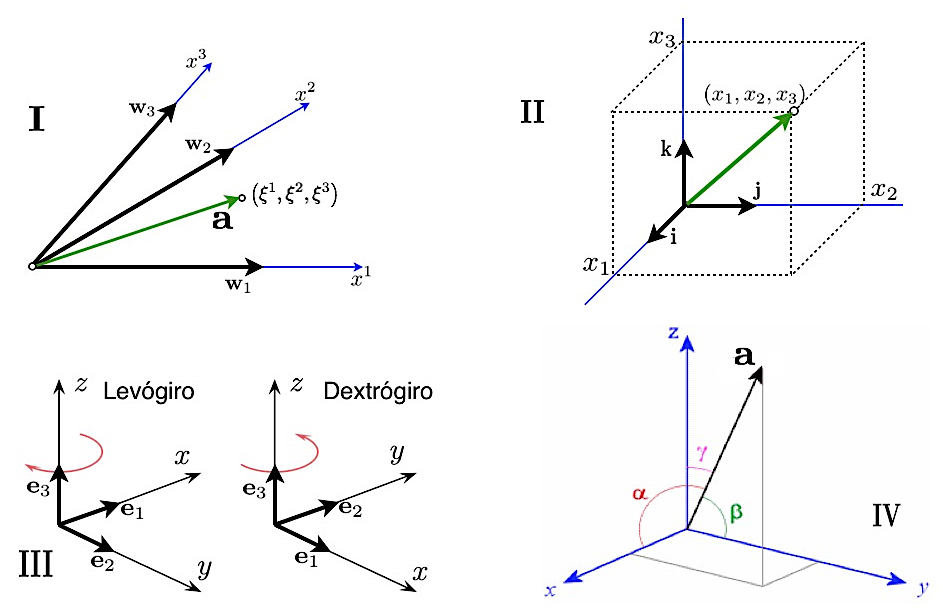
\includegraphics[height=3.0in,width=5.0in]
{VOLUMEN_1/01_Vectores_Cartesianos/Figuras/Figura1_4.jpg}
\caption{Vectores, bases y componentes}
\label{fig4vectcartes}
\end{center}
\end{figure}

Con los vectores base $\left\{{\bf w}_{1}, {\bf w}_{2}, {\bf w}_{3}\right\}  $ podemos construir un sistema (oblicuo en general) de coordenadas al colocarlos con un mismo origen, esto es:
\[
\mathbf{a}=a^{1} {\bf w}_{1}+ a^{2}{\bf w}_{2}+a^{3} {\bf w}_{3}\,,
\]
donde las cantidades $\left\{  a^{1}, a ^{2}, a^{3}\right\} $ son n�meros (no son escalares) que representan las componentes del vector ${\bf a}$ a lo largo de cada uno de los vectores base $\left\{  {\bf w}_{1}, {\bf w}_{2}, {\bf w}_{3}\right\}$. N�tese que por costumbre (la cual ser� evidente m�s adelante, en la secci�n \ref{EspacioVectorialDual}) etiquetamos estos n�meros con super�ndices y la letra que identifica al vector.

M�s a�n, cada punto $P$ del espacio viene definido por un radio vector ${\bf r} \left(P\right)  \equiv\overrightarrow{OP}$ que une el origen de coordenadas con el punto $P$ y se le asocian tres
n�meros $\left\{  {x}^{1}, {x}^{2}, {x}^{3}\right\}$, los cuales son las proyecciones a lo
largo de cada uno de los ejes coordenados $\left\{\overline{0 {x}^{1}}, \overline{0 {x}^{2}},\overline{0{x}^{3}}\right\} $.  Los n�meros $\left\{ {x}^{1}, {x}^{2},  {x}^{3}\right\} $ se denominar�n
componentes de ${\bf r} \left(  P\right)  $ en el sistema de referencia 
$\left\{ {\bf w}_{1},{\bf w}_{2},{\bf w}_{3}\right\} $.

Existe una familia de sistemas de coordenadas en la cual sus vectores base son ortogonales (o mejor
ortonormales), es decir los vectores base $\left\{ {\bf e}_{1},{\bf e}_{2},{\bf e}_{3}\right\}  $ son perpendiculares entre si. Tal y como mostraremos m�s adelante, siempre se puede construir un sistema ortogonal $\left\{  {\bf e}_{1},{\bf e}_{2},{\bf e}_{3} \right\} $ u ortonormal  
$\left\{ {\bf i}_{1}, {\bf i}_{2}, {\bf i}_{3} \right\} $ a partir de una base gen�rica de vectores
linealmente independientes $\left\{  {\bf w}_{1},{\bf w}_{2},{\bf w}_{3}\right\}$.  Cuando el sistema sea
ortogonal sus componentes se denominar�n rectangulares. Dependiendo del signo del triple producto mixto, el sistema de coordenadas ser� dextr�giro ($\left(  {\bf e}_{1}\times{\bf e}_{2}\right)  \cdot{\bf e}
_{3}>0$) o lev�giro ($\left(  {\bf e}_{1}\times{\bf e}_{2}\right) \cdot{\bf e}_{3}<0$), tal y como se muestra en el cuadrante III de la figura \ref{fig4vectcartes}.

Es costumbre ancestral\footnote{Quiz� por las arraigadas relaciones de dominaci�n de los derechos sobre los izquierdos  (en lat�n e italiano los zurdos son siniestros), o quiz� tal vez por conservar la definici�n de volumen como positivo.} utilizar la convenci�n dextr�gira donde el producto: 
$\left( {\bf e}_{1}\times{\bf e}_{2}\right) \cdot{\bf e}_{3}>0$,  y en ese caso utilizamos el bien conocido conjunto de vectores unitarios $\left\{  \mathbf{i}, \mathbf{j}, \mathbf{k} \right\}$ 
con los que ya hemos estado familiarizados: 
\[
{\bf a}=a_{x} \mathbf{i}+a_{y}\mathbf{j}+a_{z} \mathbf{k} 
\quad \text{y} \quad \mathbf{r} \left(  P\right)  =x\ \mathbf{i} +y\ \mathbf{j} +z\ \mathbf{k} \,.
\]

Tambi�n es costumbre representar  este sistema de coordenadas ortonormal
como: $\mathbf{i}  \equiv \mathbf{i}_{1},  \mathbf{j}  \equiv \mathbf{i}_{2}$ y $\mathbf{k} \equiv \mathbf{i}_{3}$  para recordar que estamos en un sistema de coordenadas cartesianas y utilizaremos los super�ndices $1,2,3$ para indicar las componentes del vector.
\[
{\bf a}=a^{1} \mathbf{i}_1 +a^{2}\mathbf{i}_2 +a^{3} \mathbf{i}_3 
\quad \text{y} \quad \mathbf{r} \left(  P\right)  =x^1\ \mathbf{i}_1 +x^2\ \mathbf{i}_2 +x^3\ \mathbf{i}_3 \,.
\]

Obviamente el m�dulo del vector se podr� expresar con la utilizaci�n del teorema de Pit�goras:
\[
\left|  {\bf a} \right|  = \sqrt{(a^{1})^{2} +(a^{2})^{2}+(a^{3})^{2}} \quad
\text{y}\quad  \left| \mathbf{r} \left(P\right)  \right| =\sqrt{(x^{1})^2+(x^{2})^2+(x^{3})^2}\,,
\]
y la multiplicaci�n por un n�mero ser�:
\[
\alpha  {\bf a}=\alpha\left(  a^{1} \mathbf{i}_1 + a^{2} \mathbf{i}_2 +a^{3}\mathbf{i}_3\right)  =
\left(  \alpha a^1\right)\mathbf{i}_1+ \left(  \alpha a^2\right) \mathbf{i}_2+\left(  \alpha a^3\right)  
\mathbf{i}_3 \,\, \Rightarrow \,\, \left| \alpha  {\bf a} \right|  =
\alpha\sqrt{(a^{1})^2+(a^{2})^2+(a^{3})^2} \,.
\]
Igualmente para un vector unitario:
\[
\hat{\bf u}_a =\dfrac{{\bf a}}{\left|  {\bf a}\right|  }=
\frac{a^1 \mathbf{i}_1 +a^2 \mathbf{i}_2 +a^3 \mathbf{i}_3}{\sqrt{(a^{1})^2 +(a^{2})^2 +(a^{3})^2 } }\,,
\]
con lo cual todo vector:
\[
{\bf a}=\left|  {\bf a}\right|  \hat{\bf u}_a = \sqrt{(a^{1})^2 +(a^{2})^2 +(a^{3})^2} \ \hat{\bf u}_a \,.
\]

\subsection{Cosenos directores}
\label{CosenosDirectores}
\index{Cosenos directores}
Como se puede apreciar en el cuadrante IV de la figura \ref{fig4vectcartes}, podemos construir tres tri�ngulos rect�ngulos con el radio vector ${\bf a}\left(P\right)$ como hipotenusa de cada uno de ellos. Los �ngulos que forma el radio vector ${\bf a}\left(P\right)$ con cada uno de los ejes coordenados $\left\{ x,y,z\right\}$ son $\left\{  \alpha ,\beta,\gamma\right\}$, respectivamente, con lo cual:
\begin{equation}
a_{x}=\left|  {\bf a}\right|  \cos(\alpha)\,,\quad a_{y}=\left|  {\bf a}\right| \cos(\beta) \quad \text{y} \quad 
a_{z}=\left|  {\bf a}\right|  \cos(\gamma) \quad  \Rightarrow \quad  \cos^{2}(\alpha)+\cos^{2}(\beta)+\cos^{2}(\gamma)=1 \,,
\label{cosdirectores}
\end{equation}
pero adem�s:
\[
\hat{\bf u}_a = \frac{{\bf a}}{\left|  {\bf a}\right|}=
\cos(\alpha)\ \mathbf{i}+\cos(\beta)\ \mathbf{j}+\cos(\gamma)\ \mathbf{k}\,.
\]


\subsection{Una divisi�n fallida}
Uno esperar�a que para cada una de las definiciones de productos vectoriales, existiera el vector cociente, es decir, que pudi�ramos ``despejar'' uno de los vectores multiplicados en t�rminos del otro. La situaci�n es que esta operaci�n no est� definida un�vocamente y lo podemos intuir a partir de una de la definici�n del producto escalar.
Supongamos que tenemos que:  $\zeta=\mathbf{a}\cdot \mathbf{b}$, con lo cual, si pudi�ramos ``despejar'', digamos, $\mathbf{b}={\zeta}/ {\mathbf{a}}$ �Tendr�amos entonces definido $\mathbf{b}$ de una manera un�voca? La respuesta es NO,  ya que $\zeta =\mathbf{a}\cdot\left( \dfrac{\zeta}{\mathbf{a}}+\mathbf{d} \right)$, donde $\mathbf{a}\ \bot\ \mathbf{d}$, por lo cual existen infinitos $\mathbf{b}=\dfrac{\zeta} {\mathbf{a}}+\mathbf{d}$ que cumplen $\zeta=\mathbf{a}\cdot\mathbf{b}$.


\subsection{Algebra vectorial en componentes}
\label{Algebravectorialycoordenadas}
\index{Algebra vectorial y coordenadas}

Es posible reescribir toda el �lgebra vectorial que hemos visto  mediante operaciones referidas a sistemas de coordenadas, como mostraremos a continuaci�n. Por simplicidad, anclaremos nuestro sistema de coordenadas a la base can�nica $\{\mathbf{i}_i\}$.

\index{Vectores 3D!Suma/resta}
Para los vectores ${\bf a}=\left(a^{1}\mathbf{i}_{1}+a^{2}\mathbf{i}_{2}+a^{3}\mathbf{i}_{3}\right)$ y ${\bf b}=\left(  b^{1} \mathbf{i}_{1}+b^{2}\mathbf{i}_{2}+b^{3}\mathbf{i}_{3}\right)$, la suma ser� representada por:
\[
{\bf a}+{\bf b}=\left(  a^{1}\mathbf{i}_{1}+a^{2}\mathbf{i}_{2}+a^{3}\mathbf{i}_{3}\right)  +\left(  b^{1} \mathbf{i}_{1}+b^{2}\mathbf{i}_{2}+b^{3}\mathbf{i}_{3}\right)  =
\left(  a^{1}+b^{1}\right)  \mathbf{i}_{1}+\left(  a^{2}+b^{2}\right)  \mathbf{i}_{2}+\left(  a^{3}+b^{3}\right)  \mathbf{i}_{3} \,,
\]
y obviamente, la resta:
\[
{\bf a}-{\bf b}=
\left(  a^{1}\mathbf{i}_{1}+a^{2}\mathbf{i}_{2}+a^{3}\mathbf{i}_{3}\right)  -\left(  b^{1}\mathbf{i}_{1}+
b^{2}\mathbf{i}_{2}+b^{3}\mathbf{i}_{3}\right)  =
\left(  a^{1}-b^{1}\right)  \mathbf{i}_{1}+\left(  a^{2}-b^{2}\right)  \mathbf{i}_{2}+\left(  a^{3}-b^{3}\right)  \mathbf{i}_{3} \,,
\]
con lo cual la distancia entre dos puntos $P$ y $M$ ser�:
\[
d\left(  P,M\right)  =\left|  \left( \mathbf{r} \left(P\right)  ={\bf a}\right)  -\left(  \mathbf{r} \left(M\right)  =
{\bf b}\right)  \right|  =\sqrt{\left( x^1-y^1\right)^{2}+\left(  x^2-y^2\right)  ^{2}+\left(  x^3-y^3 \right)  ^{2}} \,.
\]

\subsection{Dependencia e independencia lineal}
\label{IndependenciaVector3D2}
\index{Dependencia lineal!Vectores 3D}
\index{Independencia lineal!Vectores 3D}
\index{Vectores 3D!Dependencia lineal}
\index{Vectores 3D!Independencia lineal}
Ahora es f�cil estudiar la dependencia o independencia lineal en
coordenadas. Otra vez, tres vectores: 
${\bf a}=a^1 \mathbf{i}_1+ a^2\mathbf{i}_2+a^3\mathbf{i}_3 \,,
{\bf b}= b^1\mathbf{i}_1+  b^2\mathbf{i}_2+ b^3\mathbf{i}_3$ y ${\bf c}=
 c^1 \mathbf{i}_1+ c^2\mathbf{i}_2+ c^3\mathbf{i}_3$,  ser�n \textit{linealmente
independientes} si se cumple que:
\[
\alpha \ {\bf a}+\beta \ {\bf b}+\gamma \ {\bf c}= \mathbf{0} \,\, \Rightarrow \,\, \alpha=\beta=\gamma=0\,.
\]

Veamos qu� sucede para la base can�nica: $  \mathbf{i}_{1}=\mathbf{i}  \equiv \left(1,0,0\right), \mathbf{i}_{2}=\mathbf{j}  \equiv\left( 0,1,0\right),  \mathbf{i}_{3}=\mathbf{k} \equiv\left( 0,0,1\right)$. Estos vectores son claramente linealmente independientes y por lo tanto constituyen una base.


En general tendremos que:
\begin{align*}
\mathbf{0} &  =\alpha \left( a^1\mathbf{i}_1+a^2\mathbf{i}_2 +a^3 \mathbf{i}_3\right)  +
\beta \left( b^1\mathbf{i}_1+ b^2\mathbf{i}_2+ b^3\mathbf{i}_3 \right)  +
\gamma\left( c^1\mathbf{i}_1+ c^2\mathbf{i}_2+ c^3\mathbf{i}_3  \right)   
& \\
&  =
\left(  \alpha a^1+\beta  b^1+\gamma  c^1\right)  \mathbf{i}_1+
\left(  \alpha a^2+\beta  b^2+\gamma  c^2\right)  \mathbf{i}_2+
\left(  \alpha a^3+\beta  b^3+\gamma  c^3\right)  \mathbf{i}_3
\, \, \Rightarrow \, \, \left\{
\begin{array}
[c]{c}
\alpha a^1+\beta  b^1+\gamma  c^1=0\\
\alpha a^2+\beta  b^2+\gamma  c^2=0\\
\alpha a^3+\beta  b^3+\gamma  c^3=0
\end{array}
\right.
\end{align*}

Esto no es otra cosa que un sistema de 3 ecuaciones lineales con 3 inc�gnitas: $\left\{ \alpha,\beta,\gamma\right\} $, y la soluci�n que estamos buscando $\alpha=\beta=\gamma=0$ se cumplir� si:
\[
\left|
\begin{array}
[c]{ccc}
a^1 &  b^1 &  c^1\\
a^2 &  b^2 &  c^2\\
a^3 &  b^3 &  c^3
\end{array}
\right|  =
a^1 \left(  b^2 c^3- b^3 c^2\right) +
a^2 \left(  b^3 c^1- b^1 c^3\right) +
a^3 \left(  b^1 c^2- b^2 c^1\right)    \neq 0 \,.
\]

\subsection{Productos de vectores en componentes}
\subsubsection{Producto escalar}
\label{ProductoEscalar2}
\index{Producto escalar}
\index{Escalar!Producto}
\index{Vectores 3D!Producto escalar}
Ahora refrasearemos, en t�rmino de una base de vectores ortogonales, lo expresado en la secci�n \ref{ProductoEscalar1}.  Representaremos el producto escalar de dos vectores en una base cartesiana $\left\{ \mathbf{i}_1, \mathbf{i}_2,  \mathbf{i}_3 \right\}$, que es una base ortonormal, de la siguiente manera:
\[
{\bf a} \cdot{\bf b}=\left( a^1\mathbf{i}_1+a^2 \mathbf{i}_2+a^3\mathbf{i}_3 \right)  
\cdot\left(   b^1\mathbf{i}_1+ b^2\mathbf{i}_2+ b^3\mathbf{i}_3 \right)  =
a^1 b^1+a^2  b^2+a^3  b^3 \,,
\]
ya que por ser ortogonales se tiene que:
\[
\mathbf{i}_1  \cdot \mathbf{i}_1= \mathbf{i}_2 \cdot \mathbf{i}_2= \mathbf{i}_3 \cdot \mathbf{i}_3= 1 \,,
\quad \text{y} \quad
\left\{
\begin{array}
[c]{c}
\mathbf{i}_1 \cdot \mathbf{i}_2=\mathbf{i}_2 \cdot \mathbf{i}_1=0\\
\mathbf{i}_1 \cdot \mathbf{i}_3=\mathbf{i}_3 \cdot \mathbf{i}_1=0\\
\mathbf{i}_2 \cdot \mathbf{i}_3=\mathbf{i}_3 \cdot \mathbf{i}_2=0
\end{array}
\right. 
\]

Las propiedades del producto escalar en coordenadas cartesianas se comprueban f�cilmente.
\begin{itemize}
\item \textit{El producto escalar de un vector consigo mismo, siempre es positivo}. 
\[
\zeta={\bf a}\cdot{\bf a}=\left|  {\bf a}\right|  ^{2}= (a^1)^{2}+(a^2)^{2}+(a^3)^{2}\geq0 \,,
\]
y 
\[
(a^1)^{2}+(a^2)^{2}+(a^3)^{2}=0   \,\,  \Rightarrow \,\,  
a^1=a^2=a^3=0\quad\Leftrightarrow\quad{\bf a}={\bf 0}\,.
\]
Adicionalmente: $|{\bf a}| =\sqrt{\zeta}=\sqrt{{\bf a}\cdot{\bf a}}=\sqrt{(a^1)^{2}+(a^2)^{2}+(a^3)^{2}}$.

\item \textit{El producto escalar es conmutativo}.
\[
\zeta={\bf a}\cdot{\bf b}={\bf b}\cdot{\bf a}=a^1 b^1+a^2 b^2+a^3 b^3= b^1a^1+ b^2a^2+ b^3a^3\,.
\]
\item \textit{El producto escalar es distributivo}.
\[
{\bf a}\cdot\left(  {\bf b}+{\bf c}\right) = \left[ a^1\mathbf{i}_1+a^2\mathbf{i}_2 + a^3 \mathbf{i}_3\right]  \cdot   \left[  \left(  b^1+ c^1\right) \mathbf{i}_1+\left(   b^2+ c^2\right)  \mathbf{i}_2+\left(  b^3+ c^3\right)  \mathbf{i}_2\right] \,,
\]
por lo tanto:
\begin{eqnarray*}
a^1\left(  b^1+ c^1\right)  +a^2\left(   b^2+ c^2\right)  +a^3\left( b^3+ c^3\right) &=&
\left( a^1 b^1+a^1 c^1\right)  +\left(  a^2 b^2+a^2 c^2\right)+\left(  a^3 b^3+a^3 c^3\right)  \\
= \left( a^1 b^1+a^2 b^2+a^3 b^3\right)  +\left( a^1 c^1+a^2 c^2+a^3 c^3\right) &=& {\bf a}\cdot{\bf b}+{\bf a} \cdot{\bf c} \,.
\end{eqnarray*}

\item \textit{La multiplicaci�n por un escalar}.
\[
\left|  \alpha\right|  \left(  {\bf a} \cdot {\bf b}\right)  =
\left(  \alpha{\bf a}\right)  \cdot{\bf b}={\bf a}\cdot\left(\alpha{\bf b}\right)  =
\left(  \alpha a^1\right)   b^1+\left(  \alpha a^2 \right)   b^2+\left(  \alpha a^3\right)   b^3=
a^1 \left(  \alpha b^1\right)  +a^2\left(  \alpha  b^2\right)  +a^3\left(  \alpha b^3\right)\,.
\]

\item \textit{Desigualdad de Cauchy-Schwarz}.
\[
 {\bf a}\cdot{\bf b} =a^1 b^1+a^2 b^2+a^3 b^3\leq
\sqrt{(a^1)^{2} + (a^2)^{2}+ (a^3)^{2} }
\sqrt{(b^1)^{2} + (b^2)^{2}+ (b^3)^{2}}= \left|  {\bf a}\right|  \left|  {\bf b}\right|  \,.
\]

\item \textit{Diremos que dos vectores, no nulos son ortogonales (perpendiculares) si su producto escalar es nulo}. Esta afirmaci�n es inmediata:
\[
{\bf a}\ \bot\ {\bf b}\quad \Rightarrow \quad  \theta_{\left\langle {\bf a},{\bf b}\right\rangle }=
\frac{\pi}{2}\quad  \Rightarrow \quad  {\bf a}\cdot{\bf b}=
\left| {\bf a}\right|  \left|  {\bf b}\right|  \cos(\theta)_{\left\langle {\bf a}, {\bf b}\right\rangle }=0 \,, 
\]
por lo cual:
\[
a^1b^1+a^2 b^2+a^3 b^3=\left|  {\bf a}\right|  \left|  {\bf b} \right|  \cos(\theta)_{\left\langle {\bf a}, {\bf b}\right\rangle} \,\,  \Rightarrow \,\,  \cos(\theta)_{ \left\langle {\bf a}, {\bf b}\right\rangle }=\frac{a^1 b^1+a^2 b^2+a^3 b^3} {\sqrt{(a^1)^{2} + (a^2)^{2}+ (a^3)^{2} }   \sqrt{ (b^1)^{2}+ (b^2)^{2}+ (b^3)^{2}}}\,,
\]
de donde se deduce que para dos vectores perpendiculares:
\[
{\bf a}\bot{\bf b}\,\,   \Rightarrow \,\,   0=a^1 b^1+a^2 b^2+a^3 b^3 \,.
\]

\item \textit{Del producto escalar surge el teorema del coseno}.  

Es inmediato generalizar el producto escalar de un vector consigo mismo, para ello suponemos que $\bf{c}=\bf{a}+\bf{b}$, con lo cual:
\[
{\bf c}= {\bf a}+ {\bf b} \,\,  \Rightarrow \,\,  {\bf c} \cdot {\bf c}=\left(  {\bf a}+{\bf b} \right)  \cdot\left(  {\bf a}+{\bf b} \right)  \,\,  \Rightarrow \,\,   \left|  {\bf c} \right|  ^{2}=\left|  {\bf a}\right| ^{2}+\left|  {\bf b}\right|^{2}+ 2\left|  {\bf a} \right|  \left|  {\bf b}\right|  \cos(\theta)_{\left\langle{\bf a},{\bf b}\right\rangle } \,,
\]
que no es otra cosa que el teorema del coseno y est� ilustrado en el cuadrante III de la figura \ref{fig3vectcartes}.
\end{itemize}


\subsubsection{Producto vectorial}
\label{ProductoVectorial}
\index{Producto vectorial}
\index{Vectorial!Producto}
\index{Vectores 3D!Producto vectorial}
De igual manera, lo que aprendimos en la secci�n \ref{ProductorVectorial1} ahora lo expresamos en t�rminos de las componentes de los vectores en una base ortonormal de la forma:
\[
\label{produtovectorial1}
{\bf c}={\bf a}\times{\bf b}=\left( a^2 b^3-a^3 b^2\right)
\mathbf{i}_1+\left(  a^3 b^1-a^1 b^3\right)  
\mathbf{i}_2+\left( a^1 b^2-a^2 b^1\right)  \mathbf{i}_3\,,
\]
lo anterior se puede organizar como el determinante de la matriz:
\[
\label{produtovectorial2}
{\bf c}={\bf a}\times{\bf b}=\left|
\begin{array}
[c]{ccc}
\mathbf{i}_1 & \mathbf{i}_2 & \mathbf{i}_3\\
a^1 & a^2 & a^3\\
 b^1 &  b^2 &  b^3
\end{array}
\right| \,,
\]
con lo cual:
\begin{eqnarray*}
\left|  {\bf c}\right|  &=&\sqrt{\left( a^2 b^3-a^3 b^2\right) ^{2}+
\left(  a^3 b^1-a^1 b^3\right) ^{2}+\left( a^1 b^2-a^2 b^1\right)  ^{2}}\\
&=&  \sqrt{(a^1)^{2} + (a^2)^{2}+ (a^3)^{2}} \
 \sqrt{ (b^1)^{2}+ (b^2)^{2}+ (b^3)^{2}}  \operatorname*{sen}
(\theta)_{\left\langle {\bf a}, {\bf b}\right\rangle} \,.
\end{eqnarray*}

\subsubsection{Triple producto mixto}
\index{Triple producto vectorial}
\index{Producto vectorial mixto}
\index{Vectores 3D!Producto vectorial mixto}
Finalmente, analicemos el n�mero (pseudoescalar) que proviene de la multiplicaci�n:
\[
V={\bf c}\cdot\left(  {\bf a}\times{\bf b}\right)  =
\left |  {\bf c}\right | \left |  {\bf a}\times{\bf b}  \right |  \cos(\theta)
_{\left\langle {\bf c},{\bf a}\times{\bf b}\right\rangle }=\left|
\begin{array}
[c]{ccc}
 c^1 &  c^2 &  c^3\\
a^1 & a^2 & a^3\\
 b^1 &  b^2 &  b^3
\end{array}
\right| \,.
\]
Obviamente, este n�mero representa del volumen del paralelep�pedo cuyos lados quedan definidos por los vectores: ${\bf a},{\bf b}$ y ${\bf c}$.

\subsection{{\color{Fuchsia}Ejemplos}}
\label{EjemplosBase}
\begin{enumerate}
\item Si tenemos los vectores ${\bf a}={\bf i}+3{\bf j}+5{\bf k}$ y ${\bf b}=2{\bf i}+4{\bf j}+6{\bf k}$
 podemos ver que el �ngulo que forman es f�cil de calcular:
\[
\cos(\theta)=\frac{{\bf a}\cdot{\bf b}}{|{\bf a}||{\bf b}|} =
\frac{\left[{\bf i}+3{\bf j}+5{\bf k}\right] \cdot
\left[2{\bf i}+4{\bf j}+6{\bf k}\right]}
{ \sqrt{1^2+3^2+5^2} \sqrt{2^2+4^2+6^2}}=
\frac{2+12+30}{\sqrt{35} \sqrt{56}}=
\frac{44}{\sqrt{35} \sqrt{56}}=\frac{22}{\sqrt{14} \sqrt{35}} \,.
\]
Por lo tanto, $\theta=\arccos\left(\frac{22}{\sqrt{14} \sqrt{35}}\right)=0.11088$. 

Notemos que de la ecuaci�n (\ref{cosdirectores}) para los vectores ${\bf a}$ y ${\bf b}$ y su componentes resulta que: 
\[
\cos(\alpha)=\frac{a_x}{|{\bf a}|}=\frac{1}{\sqrt{35}}\,, \,\, 
\cos(\beta)=\frac{a_y}{|{\bf a}|}=\frac{3}{\sqrt{35}} \,, \,\, 
\cos(\gamma)=\frac{a_z}{|{\bf a}|}=\frac{5}{\sqrt{35}}
\,\, \Rightarrow \,\, \left[\frac{1}{\sqrt{35}}\right]^2+
\left[\frac{3}{\sqrt{35}}\right]^2+\left[\frac{5}{\sqrt{35}}\right]^2=1 \,,
\]
\[
\cos(\alpha)=\frac{b_x}{|{\bf b}|}=\frac{2}{\sqrt{56}}\,, \,\, 
\cos(\beta)=\frac{b_y}{|{\bf b}|}=\frac{4}{\sqrt{56}} \,, \,\, 
\cos(\gamma)=\frac{b_z}{|{\bf b}|}=\frac{6}{\sqrt{56}}
\,\, \Rightarrow \,\, \left[\frac{2}{\sqrt{56}}\right]^2+
\left[\frac{4}{\sqrt{56}}\right]^2+\left[\frac{6}{\sqrt{56}}\right]^2=1 \,.
\]
Y adem�s podemos ver claramente que el �ngulo entre los vectores y los cosenos directores est�n relacionados, como se muestra a continuaci�n:
\[
\cos(\theta)= 
\frac{1}{\sqrt{35}}\frac{2}{\sqrt{56}}+
\frac{3}{\sqrt{35}}\frac{4}{\sqrt{56}}+
\frac{5}{\sqrt{35}}\frac{6}{\sqrt{56}}=
\frac{22}{\sqrt{14} \sqrt{35}}\,.
\]

\item Consideremos los vectores: $
{\bf e}_{1}=\mathbf{i} \equiv \left(1,0,0\right), \  
{\bf e}_{2}=\mathbf{i}+\mathbf{j} \equiv\left(1,1,0\right), \
{\bf e}_{3}=\mathbf{i}+\mathbf{j}+\mathbf{k} \equiv\left(1,1,1\right)$.   
Al escribir el sistema de ecuaciones resulta: 
\[
\alpha=0 \,,\quad  \alpha + \beta=0\,, \quad \alpha + \beta +\gamma =0 
\,\,  \Rightarrow \,\, \alpha=0\,,\quad \beta=0 \,,\quad  \gamma=0 \,,
\]
con lo cual demostramos que son linealmente independientes y por lo tanto constituyen una base para los vectores tridimensionales.

 \item Dados los vectores: ${\bf a}={\bf i}+2{\bf j}+3{\bf k}$, ${\bf b}=4{\bf i}+5{\bf j}$  y ${\bf c}=3{\bf i}+2{\bf j}+{\bf k}$. 
 
Podemos ver que $\alpha {\bf a}+\beta {\bf b}+\gamma {\bf c}={\bf 0}$ implica que:
\[
\alpha \left[{\bf i}+2{\bf j}+3{\bf k}\right]+
\beta \left[4{\bf i}+5{\bf j}\right]+
\gamma \left[3{\bf i}+2{\bf j}+{\bf k}\right]={\bf 0}
\,\, \Rightarrow \,\,
\left\{
\begin{array}
[c]{r}
\alpha+4\beta +3\gamma =0\\
2\alpha + 5 \beta  +2\gamma =0\\
3\alpha +\gamma=0
\end{array}
\right.
\]
Cuya soluci�n es: $\alpha=\beta=\gamma=0$. Por lo tanto el conjunto $\{ {\bf a},{\bf b},{\bf c}\}$ es linealmente independiente.

Por otro lado, si queremos calcular el volumen recurrimos al triple producto vectorial:
\[
V={\bf a}\cdot\left[{\bf b}\times{\bf c}\right]=
 \left[{\bf i}+2{\bf j}+3{\bf k}\right] \cdot 
 \left[4{\bf i}+5{\bf j}\right] \times  \left[3{\bf i}+2{\bf j}+{\bf k}\right]= \left[{\bf i}+2{\bf j}+3{\bf k}\right] \cdot  
 \left[5{\bf i}-4{\bf j}-7{\bf k}\right]= -24 \,.
\]

Si tenemos un vector arbitrario, digamos, ${\bf d}=d_1{\bf i}+d_2{\bf j}+d_3{\bf k}$ y construimos las siguientes cantidades:
\[
c_1=-\frac{{\bf a}\cdot{\bf d}}{{\bf a}\cdot({\bf b} \times{\bf c})} \,,\quad
c_2 =-\frac{{\bf b}\cdot{\bf d}}{{\bf a}\cdot({\bf b} \times{\bf c})} \,,\quad
c_3= -\frac{{\bf c}\cdot{\bf d}}{{\bf a}\cdot({\bf b} \times{\bf c})}\,.
\]
resulta:
\[
c_1=\frac{d_1+2d_2+3d_3}{24} \,,\quad
c_2=\frac{4d_1+5d_2}{24}\,,\quad
c_3=\frac{3d_1+2d_2+d_3}{24}\,,
\]
y podemos ver que: $c_1 ({\bf b} \times{\bf c} )+ c_2({\bf c} \times{\bf a} ) + c_3 ({\bf a} \times{\bf b} ) + {\bf d}$, es igual a:
\begin{eqnarray*}
\frac{d_1+2d_2+3d_3}{24} (5{\bf i}-4{\bf j}-7{\bf k} )&+& 
\frac{4d_1+5d_2}{24} (4{\bf i}-8{\bf j}+4{\bf k}  ) +
\frac{3d_1+2d_2+d_3}{24} (-15{\bf i}+12{\bf j}-3{\bf k} ) \\
&+& d_1{\bf i}+d_2{\bf j}+d_3{\bf k} = {\bf 0}\,.
\end{eqnarray*}

Es decir,
\[
c_1 ({\bf b} \times{\bf c} )+ c_2({\bf c} \times{\bf a} ) + c_3 ({\bf a} \times{\bf b} ) + {\bf d}={\bf 0}\,,
\]
siempre y cuando el conjunto $\{ {\bf a},{\bf b},{\bf c}\}$ sea linealmente independiente y ${\bf d}$ un vector arbitrario. 

\end{enumerate}

\newpage
\subsection{{\color{red}Practicando con Maxima}} 
\index{Vectores con Maxima}
\index{Maxima!Vectores con}
Con el programa de manipulaci�n simb�lica {\bf Maxima} haremos algunos c�lculos sencillos con vectores. Nuevamente recomendamos ver el ap�ndice  \ref{IntroMaxima} como introducci�n al programa.

Dados los vectores, en coordenadas cartesianas: ${\bf a}={\bf i}+2{\bf j}+3{\bf k}$ y ${\bf b}=7{\bf i}+8{\bf j}+9{\bf k}$.

%%%%%% INPUT:
\begin{minipage}[t]{8ex}
{\color{red}\bf \begin{verbatim} (%i1) 
\end{verbatim}}
\end{minipage}
\begin{minipage}[t]{\textwidth}{\color{blue}
\begin{verbatim}
a:[1,2,3];
\end{verbatim}}
\end{minipage}

%%% OUTPUT:
\begin{math}\displaystyle \parbox{8ex}{\color{labelcolor}(\%o1) }
\left[ 1 , 2 , 3 \right] 
\end{math}

%%%%%% INPUT:
\begin{minipage}[t]{8ex}
{\color{red}\bf \begin{verbatim} (%i2) 
\end{verbatim}}
\end{minipage}
\begin{minipage}[t]{\textwidth}{\color{blue}
\begin{verbatim}
b:[7,8,9];
\end{verbatim}}
\end{minipage}

%%% OUTPUT:
\begin{math}\displaystyle \parbox{8ex}{\color{labelcolor}(\%o2) }
\left[ 7 , 8 , 9 \right] 
\end{math}
\newline

La multiplicaci�n por escalares y suma es simple, si queremos calcular 
$\alpha\, {\bf a} + \beta \, {\bf b}$, escribimos:

%%%%%% INPUT:
\begin{minipage}[t]{8ex}
{\color{red}\bf \begin{verbatim} (%i3) 
\end{verbatim}}
\end{minipage}
\begin{minipage}[t]{\textwidth}{\color{blue}
\begin{verbatim}
alpha*a + beta*b;
\end{verbatim}}
\end{minipage}

%%% OUTPUT:
\begin{math}\displaystyle \parbox{8ex}{\color{labelcolor}(\%o3) }
\left[ 7\,\beta+\alpha , 8\,\beta+2\,\alpha , 9\,\beta+3\,\alpha
  \right] 
\end{math}
\newline 

Para el producto escalar procedemos utilizando el operador punto,  como se muestra a continuaci�n.

%%%%%% INPUT:
\begin{minipage}[t]{8ex}
{\color{red}\bf \begin{verbatim} (%i4) 
\end{verbatim}}
\end{minipage}
\begin{minipage}[t]{\textwidth}{\color{blue}
\begin{verbatim}
a.b;
\end{verbatim}}
\end{minipage}

%%% OUTPUT:
\begin{math}\displaystyle \parbox{8ex}{\color{labelcolor}(\%o4) }
50
\end{math}
\newline 

El c�lculo de producto vectorial no es tan obvio, debemos cargar previamente la librer�a {\bf vect}. 
%%%%%%%%%
\index{Maxima!\texttt{vect}}
\index{\texttt{vect}}
%%%%%%%%%

%%%%%% INPUT:
\begin{minipage}[t]{8ex}
{\color{red}\bf \begin{verbatim} (%i5) 
\end{verbatim}}
\end{minipage}
\begin{minipage}[t]{\textwidth}{\color{blue}
\begin{verbatim}
load(vect)$
\end{verbatim}}
\end{minipage}
\newline

El operador para el producto vectorial es una tilde  y adem�s debemos utilizar la funci�n {\bf express}. Entonces, para calcular ${\bf a} \times {\bf b}$, ejecutamos los siguientes comandos:

%%%%%% INPUT:
\begin{minipage}[t]{8ex}
{\color{red}\bf \begin{verbatim} (%i6) 
\end{verbatim}}
\end{minipage}
\begin{minipage}[t]{\textwidth}{\color{blue}
\begin{verbatim}
express(a~b);
\end{verbatim}}
\end{minipage}

%%% OUTPUT:
\begin{math}\displaystyle \parbox{8ex}{\color{labelcolor}(\%o6) }
\left[ -6 , 12 , -6 \right] 
\end{math}
\newline

La norma de un vector, como ya vimos, es:  $\sqrt{{\bf a} \cdot {\bf a}}$

%%%%%% INPUT:
\begin{minipage}[t]{8ex}
{\color{red}\bf \begin{verbatim} (%i7) 
\end{verbatim}}
\end{minipage}
\begin{minipage}[t]{\textwidth}{\color{blue}
\begin{verbatim}
sqrt(a.a);
\end{verbatim}}
\end{minipage}

%%% OUTPUT:
\begin{math}\displaystyle \parbox{8ex}{\color{labelcolor}(\%o7) }
\sqrt{14}
\end{math}
\newline

Si tenemos otro vector, digamos ${\bf c}=-4{\bf i}+5{\bf j}-6{\bf k}$, el producto triple: ${\bf a}\cdot{\bf b}\times{\bf c}$ se calcula as�:

%%%%%% INPUT:
\begin{minipage}[t]{8ex}
{\color{red}\bf \begin{verbatim} (%i8) 
\end{verbatim}}
\end{minipage}
\begin{minipage}[t]{\textwidth}{\color{blue}
\begin{verbatim}
c:[-4,5,-6];
\end{verbatim}}
\end{minipage}

%%% OUTPUT:
\begin{math}\displaystyle \parbox{8ex}{\color{labelcolor}(\%o8) }
\left[ -4 , 5 , -6 \right]
\end{math}

%%%%%% INPUT:
\begin{minipage}[t]{8ex}
{\color{red}\bf \begin{verbatim} (%i9) 
\end{verbatim}}
\end{minipage}
\begin{minipage}[t]{\textwidth}{\color{blue}
\begin{verbatim}
a.express(b~c);
\end{verbatim}}
\end{minipage}

%%% OUTPUT:
\begin{math}\displaystyle \parbox{8ex}{\color{labelcolor}(\%o9) }
120
\end{math}
\newline

El �ngulo entre los vectores ${\bf a}$ y ${\bf b}$, es:
\[
\theta=\arccos\left(\frac{{\bf a}\cdot {\bf b}}{|{\bf a}| |{\bf b}|}\right)\,.
\]
En {\bf Maxima} usamos la funci�n {\bf acos(x)}   para el  $\mbox{arcocoseno}(x)$.  Consultar el manual del programa para ver el resto de las funciones trigonom�tricas. 

%%%%%% INPUT:
\begin{minipage}[t]{8ex}
{\color{red}\bf \begin{verbatim} (%i10) 
\end{verbatim}}
\end{minipage}
\begin{minipage}[t]{\textwidth}{\color{blue}
\begin{verbatim}
acos((a.b)/(sqrt(a.a)*sqrt(b.b)));
\end{verbatim}}
\end{minipage}

%%% OUTPUT:
\begin{math}\displaystyle \parbox{8ex}{\color{labelcolor}(\%o10)}
\mbox{acos} \left(\frac{50}{\sqrt{14}\,\sqrt{194}}\right)
\end{math}
\newline

Seguramente lo queremos es el valor num�rico, esto se hace agregando  la funci�n {\bf float}.  Con la siguiente sintaxis logramos el objetivo:

%%%%%% INPUT:
\begin{minipage}[t]{8ex}
{\color{red}\bf \begin{verbatim} (%i11) 
\end{verbatim}}
\end{minipage}
\begin{minipage}[t]{\textwidth}{\color{blue}
\begin{verbatim}
acos((a.b)/(sqrt(a.a)*sqrt(b.b))),float;
\end{verbatim}}
\end{minipage}

%%% OUTPUT:
\begin{math}\displaystyle \parbox{8ex}{\color{labelcolor}(\%o11) }
0.2858867976945064
\end{math}
\newline

Para finalizar, podemos considerar el problema de la independencia lineal de vectores. Tomemos el conjunto de vectores del ejemplo \ref{EjemplosBase}, es decir, los vectores: ${\bf a}={\bf i}+2{\bf j}+3{\bf k}$, ${\bf b}=4{\bf i}+5{\bf j}$ y ${\bf c}=3{\bf i}+2{\bf j}+{\bf k}$. El sistema de ecuaciones a resolver era:
\[
\left\{
\begin{array}
[c]{r}
\alpha+4\beta +3\gamma =0\\
2\alpha + 5 \beta  +2\gamma =0\\
3\alpha +\gamma=0
\end{array}
\right.
\]

Disponemos de un comando que permite resolver sistemas de ecuaciones lineales, este comando se llama {\bf linsolve}.  Podemos escribir el sistema de ecuaciones como una lista y luego resolver: 
 %%%%%%%%%
\index{Maxima!\texttt{linsolve}}
%%%%%%%%%

%%%%%% INPUT:
\begin{minipage}[t]{8ex}
{\color{red}\bf \begin{verbatim} (%i12)  \end{verbatim}}
\end{minipage}
\begin{minipage}[t]{\textwidth}{\color{blue}
\begin{verbatim}
ecus:[alpha+4*beta+3*gamma=0,2*alpha+5*beta+2*gamma=0,3*alpha+gamma=0];
\end{verbatim}}
\end{minipage}

%%% OUTPUT:
\begin{math}\displaystyle \parbox{8ex}{\color{labelcolor}(\%o12) }
\left[ 3\,\gamma+4\,\beta+\alpha=0 , 2\,\gamma+5\,\beta+2\,\alpha=0 , \gamma+3\,\alpha=0 \right]
\end{math}

%%%%%% INPUT:
\begin{minipage}[t]{8ex}
{\color{red}\bf \begin{verbatim} (%i13)  \end{verbatim}}
\end{minipage}
\begin{minipage}[t]{\textwidth}{\color{blue}
\begin{verbatim}
linsolve(ecus,[alpha,beta,gamma]);
\end{verbatim}}
\end{minipage}

%%% OUTPUT:
\begin{math}\displaystyle \parbox{8ex}{\color{labelcolor}(\%o13) }
\left[ \alpha=0 , \beta=0 , \gamma=0 \right]
\end{math}

\begin{center}
{\color{red}\rule{15.8cm}{0.4mm}}
\end{center}


\subsection{{\color{OliveGreen}Ejercicios}}

\begin{enumerate}
\item Con la definici�n del producto escalar entre vectores, demuestre que si $\theta$ es el �ngulo entre los vectores ${\bf a}$ y ${\bf b}$, entonces:
\[
\cos(\theta)=\frac{a_1b_1}{ab}+\frac{a_2b_2}{ab}+\frac{a_3b_3}{ab}\,.
\]
Donde las cantidades $a_i/a$ y $b_i/b$ son los cosenos directores de  ${\bf a}$ y ${\bf b}$ respectivamente. 

\item Encuentre la distancia del punto $P$ al origen, si $P$ viene dado por el vector posici�n: $\mathbf{r}= 2\mathbf{i}+4\mathbf{j}-3\mathbf{k}$. Y si para un punto arbitrario el vector posici�n es: $\mathbf{r}= x\mathbf{i}+y\mathbf{j}+z\mathbf{k}$ �Qu� superficie describe �ste vector cuando $|\mathbf{r}|=3$? 

\item Encuentre los cosenos directores y los correspondientes  �ngulos para los siguientes vectores:
\begin{enumerate}
\item ${\bf a}={\bf i}+{\bf j}+{\bf k}$.
\item ${\bf b}={\bf i}-2{\bf j}+2{\bf k}$.
\item ${\bf c}=4{\bf i}-2{\bf j}+3{\bf k}$.
\end{enumerate}

\item Sea $\{ {\bf i}_1, {\bf i}_2, {\bf i}_3\}$ una base ortonormal  dextr�gira. Verifique que los vectores:
\[
{\bf a}= {\bf i}+2{\bf j}+3{\bf k} \,,\quad   {\bf b}= {\bf i}+5{\bf j} \,,\quad 
{\bf c}= 3{\bf i}+2{\bf j}+{\bf k} \,.
\]
forman una base �Esta base ser� del tipo dextr�giro o lev�giro?

\item Sea $\{ {\bf i}_1, {\bf i}_2, {\bf i}_3\}$ una base ortonormal �Son los siguientes conjuntos de vectores una base? 
\begin{enumerate}
\item $
{\bf a}_1= 2{\bf i}+{\bf j}-3{\bf k} \,,\quad   
{\bf a}_2= {\bf i}-4{\bf k} \,,\quad 
{\bf a}_3= 4{\bf i}+3{\bf j}-{\bf k}$.
\item $
{\bf b}_1= {\bf i}-3{\bf j}+2{\bf k} \,,\quad   
{\bf b}_2= 2{\bf i}-4{\bf j}-{\bf k} \,,\quad 
{\bf b}_3= 3{\bf i}+2{\bf j}-{\bf k}$.
\end{enumerate}


\item Dados los vectores: 
\[
{\bf a}= {\bf i}_1+2{\bf i}_2+3{\bf i}_3\,, \quad
{\bf b}= 4{\bf i}_1+5{\bf i}_2+6{\bf i}_3\,, \quad
{\bf c}= 3{\bf i}_1+2{\bf i}_2+ {\bf i}_3\,, \quad
{\bf d}= 6{\bf i}_1+5{\bf i}_2+4{\bf i}_3 \,.
\]
\begin{enumerate}
\item Encuentre: 
\[
{\bf a} +{\bf b} + {\bf c} + {\bf d} \,,\quad 
{\bf a} +{\bf b} - {\bf c} - {\bf d} \,,\quad
\mathbf{a} -\mathbf{b} + \mathbf{c} - \mathbf{d} \,,\quad
-\mathbf{a} +\mathbf{b} - \mathbf{c} + \mathbf{d} \,.
\]
\item El �ngulo entre los vectores $\mathbf{a}, \mathbf{b}, \mathbf{c}, \mathbf{d}$ y  los vectores base ${\bf i}_1, {\bf i}_2, {\bf i}_3$.
\item La magnitud de los vectores  $\mathbf{a}, \mathbf{b}, \mathbf{c}, \mathbf{d}$.
\item El �ngulo entre $\mathbf{a}$ y $\mathbf{b}$ y entre $\mathbf{c}$ y $\mathbf{d}$.
\item La proyecci�n  de $\mathbf{a}$ sobre $\mathbf{b}$.
\item �Son los vectores $\mathbf{a}, \mathbf{b}, \mathbf{c}, \mathbf{d}$  coplanares?
\item Encuentre $(\mathbf{a}+\mathbf{b})\cdot (\mathbf{c}+\mathbf{d})$.
\item Los productos  $\mathbf{a} \times \mathbf{b}$,  $\mathbf{b} \times \mathbf{c}$,
 $\mathbf{c} \times \mathbf{d}$ y los �ngulos que estos forman con $\mathbf{d}$.
\item $\mathbf{c}\cdot (\mathbf{a} \times \mathbf{b})$.
\end{enumerate}

\item Verifique la desigualdad triangular: $|{\bf a}+{\bf b}|\leq |{\bf a}|+|{\bf b}|$, para los siguientes vectores:
\begin{enumerate}
\item ${\bf a}={\bf i}+2{\bf j}+3{\bf k} $ y $ {\bf b}=2{\bf i}+{\bf j}+7{\bf k}$.
\item ${\bf a}=2{\bf i}-{\bf j}-2{\bf k} $ y $ {\bf b}=3{\bf i}+2{\bf j}+3{\bf k}$.
\end{enumerate}

\item Si ${\bf a}$ y ${\bf b}$ son vectores arbitrarios y $\alpha$ y $\beta$ n�meros, demuestre que:
\[
|\alpha {\bf a}+\beta{\bf b}|^2 \leq \alpha^2| {\bf a}|^2+2\alpha\beta
({\bf a}\cdot{\bf b})+\beta^2|{\bf b}|^2\,.
\]
\item Si ${\bf a}, {\bf b}, {\bf c}$ y ${\bf d}$ son vectores arbitrarios y $\alpha, \beta, \gamma$ escalares que satisfacen:
\[
\alpha ({\bf b} \times{\bf c} )+ \beta ({\bf c} \times{\bf a} ) +
\gamma ({\bf a} \times{\bf b} ) + {\bf d} ={\bf 0}\,,
\]
demuestre que si ${\bf a}, {\bf b}$ y ${\bf c}$ son linealmente independientes, entonces: 
\[
\alpha=-\frac{{\bf a}\cdot{\bf d}}{{\bf a}\cdot({\bf b} \times{\bf c})} \,,\quad
\beta =-\frac{{\bf b}\cdot{\bf d}}{{\bf a}\cdot({\bf b} \times{\bf c})} \,,\quad
\gamma= -\frac{{\bf c}\cdot{\bf d}}{{\bf a}\cdot({\bf b} \times{\bf c})}\,.
\]
\item Si ${\bf a}, {\bf b}, {\bf c}$ y ${\bf d}$ son vectores arbitrarios y $\alpha, \beta, \gamma$ escalares que satisfacen:
\[
\alpha {\bf a}+ \beta {\bf b}+\gamma {\bf c} + {\bf d} ={\bf 0}\,,
\]
demuestre que si ${\bf a}, {\bf b}$ y ${\bf c}$ son linealmente independientes, entonces: 
\[
\alpha=-\frac{{\bf d}\cdot({\bf b} \times{\bf c})}{{\bf a}\cdot({\bf b} \times{\bf c})} \,,\quad
\beta =-\frac{{\bf d}\cdot({\bf c} \times{\bf a})}{{\bf a}\cdot({\bf b} \times{\bf c})} \,,\quad
\gamma= -\frac{{\bf d}\cdot({\bf a} \times{\bf b})}{{\bf a}\cdot({\bf b} \times{\bf c})}\,.
\]
Ayuda: tome el producto escalar de la ecuaci�n con ${\bf b} \times{\bf c}$, ${\bf a} \times{\bf c}$ y ${\bf a} \times{\bf b}$.

\item Demuestre que los vectores ${\bf a}={\bf i}+2{\bf j}+{\bf k}$, ${\bf b}=2{\bf i}-{\bf j}-{\bf k}$ y ${\bf c}=4{\bf i}+3{\bf j}+{\bf k}$ son linealmente independientes. Escoja un vector ${\bf d}$ y verifique los resultados de los dos �ltimos ejercicios. 

\item Utilizando {\bf Maxima} realice todos los ejercicios anteriores y compare los resultados.


\end{enumerate}

\section{Aplicaciones del �lgebra vectorial}
\label{AplicacionesAlgebraVectorial}
\index{Aplicaciones!�lgebra vectorial} 
\index{�lgebra vectorial!Aplicaciones} 

Uno de los terrenos m�s exitosos de las aplicaciones del �lgebra vectorial es la geometr�a anal�tica. Esto se realiza en base a la definici�n que hici�ramos del radio vector, en la cual a cada punto, 
$P$, del espacio le asoci�bamos un radio vector posici�n tal y como lo mostramos en el cuadrante I de la figura \ref{fig4vectcartes}.
\[
P\longleftrightarrow(x,y,z)  \equiv\left(  x^{1},x^{2}
,x^{3}\right)  \,\,  \Rightarrow \,\,  {\bf r}\left(  P\right)  =
x\ \mathbf{i}+y\ \mathbf{j}+z\ \mathbf{{k}}=
x^{1}\mathbf{i}_{1}+x^{2}\mathbf{i}_{2}+
x^{3}\mathbf{i}_{3}=\sum_{i=1}^3 x^{i}\mathbf{i}_{i}\,.
\]
A partir de esta definici�n todas las propiedades geom�tricas del
espacio las podemos construir con vectores.


\subsection{Rectas y vectores}
\label{RectasVectores}
\index{Rectas y vectores}
\index{Vectores 3D!Rectas}
La ecuaci�n de la recta en t�rmino de vectores la definiremos fijando uno de sus puntos, digamos: 
\[
{\bf r}\left( P_{1}\right)  \equiv {\bf x} \left(  P_{1}\right)  ={\bf x}_{1}= 
x_1\ \mathbf{{i} }+y_1\ \mathbf{{j} }+z_1\ \mathbf{{k} }=
x_{(1)}^{1} \mathbf{{i} }_{1}+
x_{(1)}^{2} \mathbf{{i} }_{2}+
x_{(1)}^{3} \mathbf{{i} }_{3} \longleftrightarrow \left(x_{1},y_{1},z_{1}\right) \, ,
\]
y un vector que indique su direcci�n, digamos $\mathbf{a} =a^{1}\mathbf{{i}}+a^{2}\mathbf{{j} } +a^3 \mathbf{{k}}$ (ver cuadrante I de la figura \ref{fig5vectcartes}) con lo cual la ecuaci�n de una recta en lenguaje vectorial ser�:
\[
{\bf x} ={\bf x} _{1}+\lambda \mathbf{a}  \,\,  \Rightarrow \,\,  x_{1} \mathbf{{i} }+y_{1}\mathbf{{j} }+z_{1} \mathbf{{k} } +\,  \lambda\left(a^{1} \mathbf{{i} }+a^{2} \mathbf{{j} }+a^{3} \mathbf{{k}}\right) \,\,  \Rightarrow \,\, \left\{
\begin{array}
[c]{c}
x=x_{1}+\lambda a^{1}\\ \\
y=y_{1}+\lambda a^{2}\\ \\
z=z_{1}+\lambda a^{3} 
\end{array}
\right. 
\]
donde $\mathbf{x} =x\ \mathbf{{i} }+y\ \mathbf{{j} }+z\ \mathbf{{k} }$ es  el conjunto de puntos gen�ricos que cumple con la ecuaci�n de la recta en 3D. 

\begin{figure}[t]
\begin{center}
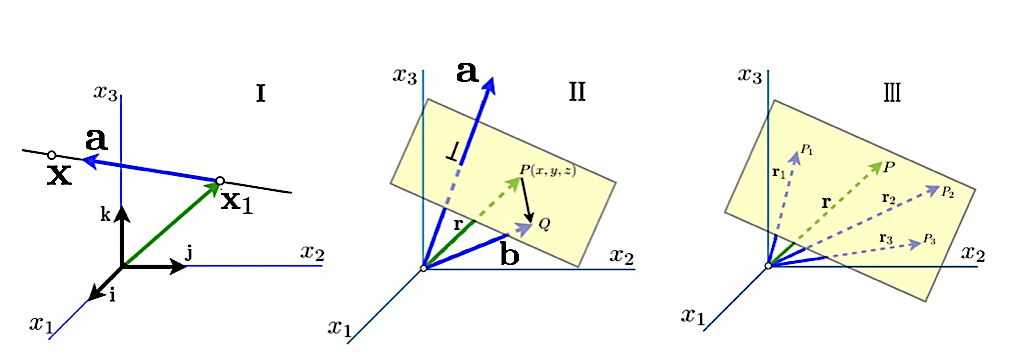
\includegraphics[height=2.5in,width=6.5in]
{VOLUMEN_1/01_Vectores_Cartesianos/Figuras/Figura1_5.jpg}
\caption{Geometr�a anal�tica y vectores cartesianos}
\label{fig5vectcartes}
\end{center}
\end{figure}

Existe una manera m�s elegante, como veremos en la secci�n siguiente, de reescribir las ecuaciones anteriores utilizando la notaci�n de �ndices\footnote{Quitaremos aqu� el s�mbolo de sumatoria, esta convenci�n quedar� clara en la siguiente secci�n, pero mantengamos en mente que tenemos una suma sobre el �ndice $i$.}.  Las ecuaciones ahora son m�s evidentes:
\[
{\bf x} ={\bf x} _{1}+\lambda\mathbf{a} \,\,  \Rightarrow \,\,  x^{i}\mathbf{{i} }_{i}=
x_{(1)}^{i}\mathbf{{i} }_{i}+\lambda a^{i}\mathbf{{i} }_{i} \,\,  \Rightarrow \,\,  
x^{i}=x_{(1)}^{i}+\lambda a^{i}\,,\qquad \text{para }\, i=1,2,3 \, .
\]
donde: $\left(x, y, z\right)\equiv \left(x^1,  x^2, x^3\right)$ y 
$\left(\mathbf{i}, \mathbf{j}, \mathbf{k}\right)\equiv \left(\mathbf{i}_1,  \mathbf{i}_2, \mathbf{i}_3\right)$.

N�tese que efectivamente se cumplen tres ecuaciones escalares y cada una de ellas tiene la forma de una recta.
Adem�s, tal y como se muestra la figura \ref{fig5vectcartes} el punto gen�rico $\left(x,y,z\right) $ lo describe (sobre la recta) la variaci�n del m�dulo de $\mathbf{a}$ mediante la constante de proporcionalidad $\lambda.$ Si se requiere describir una recta que pase por dos puntos: $\left(x_{1},y_{1},z_{1}\right)$ y $\left(  x_{2},y_{2},z_{2}\right)$ entonces una vez seleccionado uno de los puntos (digamos $\left(  x_{1}, y_{1}, z_{1}\right) $) seleccionamos el vector $\mathbf{a} ={\bf r} \left(P_{2}\right)  - {\bf r}\left(  P_{1}\right)$ como la resta de los dos radio vectores a los puntos $P_{2}$ y $P_{1}$. Esto es:
\[
{\bf x} ={\bf x} _{1}+\lambda\left(  {\bf x} _{2}-{\bf x} _{1}\right) \,.
\]

Al despejar $\lambda$ de la ecuaciones de las rectas resulta:
\[
x^{i}=x_{(1)}^{i}+\lambda a^{i} \,\, \Rightarrow \,\, \lambda=
\frac{x^{i}-x_{(1)}^{i}}{a^{i}} =\frac{x-x_{1}}{a^{1}}=\frac{y-y_{1}}{a^{2}}=\frac{z-z_{1}}{a^{3}}\,,
\]
y de manera  equivalente:
\[
x^{i}=x_{(1)}^{i}+\lambda\left(  x_{(2)}^{i}-x_{(1)}^{i}\right)  
\,\, \Rightarrow \,\, 
\lambda=\frac{x^{i}-x_{(1)}^{i}}{x_{(2)}^{i}-x_{(1)}^{i}}=
\frac{x-x_{1}}{x_{2}-x_{1}}=\frac{y-y_{1}}{y_{2}-y_{1}}=\frac{z-z_{1}}{z_{2}-z_{1}}\,.
\]

\subsection{Planos y vectores}
\label{PlanosVectores}
\index{Planos y vectores}
\index{Vectores 3D!Planos}
Ocurre exactamente lo mismo cuando construimos la ecuaci�n vectorial para un plano. En general una superficie la define su vector normal (perpendicular). En el caso de una superficie plana (un plano) tendr� una �nica normal
que lo define, por lo tanto, un plano vendr� definido por su vector perpendicular en un punto, digamos $Q=P_{1}: \left( x_{1},y_{1},z_{1}\right)$.  La ecuaci�n vectorial del plano vendr� definida por todos los vectores $\overrightarrow{PQ}$ tales que sean perpendiculares a un determinado vector ${\bf a}$ (ver cuadrante II de la figura \ref{fig5vectcartes}). Donde el punto $P$ es un punto gen�rico $\left(x,y,z\right)$ que define un radio vector. La ecuaci�n  vectorial del plano ser� simplemente: 
\[
\mathbf{a} \cdot \overrightarrow{PQ}=
\mathbf{a} \cdot \left[ {\bf r} \left(  P\right)  -\underset{\bf{b}}{\underbrace{{\bf r} \left(  P_{1}\right)  }}\right]  =0
 \quad \Leftrightarrow \quad \mathbf{a} \cdot \left(  {\bf r} -{\bf r} _{1}\right)  =0
 \quad\Leftrightarrow \quad\mathbf{a} \cdot{\bf r} =
 \underset{b}{\underbrace{\mathbf{a} \cdot{\bf r} _{1}}}\,.
\]
Esto es, se tiene que cumplir la condici�n:
\begin{align*}
\left(  a^{1}\ \mathbf{{i} }+a^{2}\ \mathbf{{j} } +a^{3}\ \mathbf{{k} }\right)  \cdot \left[ \left(  x\ \mathbf{{i} }+y\ \mathbf{{j} }+z\ \mathbf{{k} }\right)  -\left(  x_{1}
\ \mathbf{{i} }+y_{1}\ \mathbf{{j} }+z_{1}\ \mathbf{{k} }\right)  \right]  &  =0\\
\left(  a^{1}\ \mathbf{{i} } +a^{2}\ \mathbf{{j} } +a^{3}\ \mathbf{{k} }\right)  \cdot\left[  \left(  x-x_{1}\right)
\ \mathbf{{i} }+\left(  y-y_{1}\right)  \mathbf{{j} }+\left(z-z_{1}\right)  \mathbf{{k} }\right]   &  =0\\
a^{1}\left(  x-x_{1}\right)  +a^{2}\left(  y-y_{1}\right)  +a^{3}\left( z-z_{1}\right)   &  =0 \,,
\end{align*}
con lo cual, la ecuaci�n del plano queda como siempre la hemos conocido:
\[
a^{1}x+a^{2}y+a^{3}z-a^{1}x_{1}-a^{2}y_{1}-a^{3}z_{1}=0 \,\,  \Rightarrow \,\,
a^{1}x+a^{2}y+a^{3}z=b=a^{1}x_{1}+a^{2}y_{1}+a^{3}z_{1}\,.
\]

Nuevamente, de manera  compacta:
\[
a^{i}x_{i}-a^{j}x_{j(1)}=0\,\,  \Rightarrow \,\,  a_{k}x^{k}=b=a_{l}x_{(1)}^{l}\,.
\]

Es claro que ${\bf a} \cdot{\bf r} _{1}=b$ es la proyecci�n del radio vector ${\bf r} \left(  P_{1}\right)  $ sobre la perpendicular que define al plano. Por lo tanto ser� la distancia entre el plano y el origen de coordenadas. Si $b=0$ el plano pasa por el origen de coordenadas.

Consideremos ahora el cuadrante III de la figura \ref{fig5vectcartes}. All� est�n especificados tres puntos en el espacio caracterizados por sus correspondientes radio vectores posici�n: ${\bf r} \left(  P_{1}\right)={\bf r} _{1},{\bf r} \left(  P_{2}\right)  ={\bf r} _{2}$ y ${\bf r} \left(P_{3}\right)  ={\bf r} _{3}$. Estos tres puntos ser�n coplanares si:
\[
\left(  {\bf r} _{1}-{\bf r} _{2}\right)  \cdot\left[  \left(  {\bf r} _{2}-{\bf r} _{3}\right)  \times\left(  {\bf r} _{3}-{\bf r} _{1}\right)  \right] =0\quad \Leftrightarrow \quad 
\varepsilon_{mnl}\left(  x_{1}^{m}-x_{2}^{m}\right)  \left(  x_{2}^{n}-x_{3}^{n}\right)  \left(  x_{3}^{l}-x_{1}
^{l}\right)  =0\,,
\]
y la ecuaci�n vectorial del plano vendr� dada por:
\[
\left(  {\bf r} -{\bf r} _{1}\right)  \cdot\left[ \left(  {\bf r} _{2}-{\bf r}_{1}\right)  
\times\left(  {\bf r} _{3}-{\bf r} _{1}\right)  \right]=0 \,.
\]

\subsection{{\color{Fuchsia}Ejemplos}}
\label{EjemploPlanos}
\begin{enumerate}
\item Un plano viene determinado por los puntos $A=(1,1,1)$, $B=(1,2,3)$ y $C=(0,0,0)$. Para encontrar la ecuaci�n del plano podemos hacer lo siguiente: Encontremos el vector posici�n de los puntos $A$ y $B$, 
\[
{\bf r}_{AB}={B}-{A}=(0,1,2)\,, \quad {\bf r}_{AC}={C}-{A}=(-1,-1,-1)\,,
\]
un vector normal al plano es: ${\bf n}={\bf r} _{AB}\times {\bf r} _{AC}=(1,-2,1)$.

Para la ecuaci�n del plano, podemos escoger el vector  $\mathbf{a}=(1,1,1)$ por lo que tenemos entonces que:
\[
{\bf n}\cdot{\bf r} = {\bf n}\cdot\mathbf{a} \,\,  \Rightarrow \,\,   
(1,-2,1)\cdot (x,y,z)=(1,-2,1)\cdot (1,1,1) \,\,  \Rightarrow \,\, 
x-2y+z=0\,.
\]


\item  Dados los siguientes puntos en el espacio: $(1,0,3)$, $( 2,-1,0 )$, $( 0,-1,1)$, $(-1,0,1)$.

Consideremos los tres primeros puntos, que podemos considerar coplanares ya que bastan tres puntos para definir un plano. 
Estos tres puntos son los vertices de un tri�ngulo cuya �rea podemos calcular de la siguiente manera:

Primero seleccionamos uno de los puntos como un v�rtice privilegiado (digamos $( 2,-1,0 )$) respecto al cual construiremos dos vectores que representan dos de los lados del tri�ngulo. Esto es:
\[
{\bf a} = (1,0,3) - ( 2,-1,0 ) \leftrightarrow {\bf a} = - {\bf i} +{\bf j} +3 {{\bf k}}\,,\quad
{\bf b} = (0,-1,1) - ( 2,-1,0 )  \leftrightarrow {\bf b} = -2{\bf i}   +{{\bf k}}\,,
\]
con lo cual, el �rea del tri�ngulo ser� la mitad del �rea del paralelogramo que tiene por lados estos dos vectores. Es decir:
\[
A = \frac{1}{2} | {\bf a} \times {\bf b} | \,\,  \Rightarrow \,\,  {\bf a} \times {\bf b} = \left|\begin{array}{ccc}{\bf i} & {\bf j} & {{\bf k}} \\-1 & 1 & 3 \\-2 & 0 & 1\end{array}\right| = {\bf i} -5 {\bf j} +2{{\bf k}} \,\,  \Rightarrow \,\, A = \frac{1}{2}| {\bf i} -5 {\bf j} +2{{\bf k}}|=\frac{\sqrt{30}}{2}\,.
\]

Por otro lado, la ecuaci�n del plano que generan estos tres puntos se calcula con la siguiente ecuaci�n:
\[
\left(  {\bf r}-{\bf r}_{1}\right)  \cdot \left(  \left(  {\bf r}_{2}-{\bf r}_{1}\right)  \times\left(  {\bf r}_{3}-{\bf r}_{1}\right)  \right) =0\,,
\]
donde:
\[
{\bf r} = x {\bf i} + y{\bf j} + z {{\bf k}}, \quad {\bf r}_{1} =  {\bf i}  + 3 {{\bf k}}, \quad {\bf r}_{2} = 2 {\bf i} -{\bf j}, \quad {\bf r}_{3} =  -{\bf j} + {{\bf k}},
\]
con lo cual la ecuaci�n del plano queda como:
\[
\left|\begin{array}{ccc}(x -1) & y  & (z - 3) \\1 & -1 & -3 \\-1 & -1 & -2\end{array}\right|=0  \,\, \Rightarrow \,\,
 -(x -1) + 5y -2(z -3) = 0 \,\, \Rightarrow \,\, x -5y +2z = 7\,.
\]

Podemos verificar si el cuarto punto, $(-1,0,1)$, se encuentra en el plano, es decir, debemos verificar que cumple la ecuaci�n que lo define. 
\[
x -5y +2z = 7 \,\, \Rightarrow \,\,(-1) -5(0) +2(1) \neq 7\,,
\]
por lo tanto, los cuatro puntos no son coplanares. Podemos entonces  calcular la distancia del cuarto punto al plano construyendo un vector unitario normal al plano.
\[
\hat{\bf n}_{P} = \frac{{\bf a} \times {\bf b} }{| {\bf a} \times {\bf b}|} =\frac{1}{\sqrt{30}} \left(  {\bf i} -5 {\bf j} +2{\bf k} \right) \,,
\]
con lo cual la distancia al cuarto punto ser�:
\[
d =  \hat{\bf n}_{P}  \cdot {\bf c} = \frac{1}{\sqrt{30}} \left(  {\bf i} -5 {\bf j} +2{\bf k} \right) \cdot \left( -3 {\bf i}  +{\bf j} + {\bf k}\right) = -\frac{6}{\sqrt{30}}\,.
\]
\end{enumerate}

\newpage
\subsection{{\color{red}Practicando con Maxima}} 

Consideremos el plano determinado por los puntos $P=(1, 1, 1)$, $Q=(2, 4, 6)$ y $R=(2, 2, 2)$. Para construir la ecuaci�n del plano primero ingresamos los vectores posici�n de cada punto. 
Tambi�n incorporaremos las librer�as {\bf vect} y {\bf draw} que necesitaremos.
%%%%%%%%%%%%%%
\index{Maxima!\texttt{draw}}
\index{\texttt{draw}}
%%%%%%%%%%%%%%

%%%%%% INPUT:
\begin{minipage}[t]{8ex}
{\color{red}\bf \begin{verbatim} (%i1) 
\end{verbatim}}
\end{minipage}
\begin{minipage}[t]{\textwidth}{\color{blue}
\begin{verbatim}
load(vect)$ load(draw)$
\end{verbatim}}
\end{minipage}

%%%%%% INPUT:
\begin{minipage}[t]{8ex}
{\color{red}\bf \begin{verbatim} (%i2) 
\end{verbatim}}
\end{minipage}
\begin{minipage}[t]{\textwidth}{\color{blue}
\begin{verbatim}
P:[1,1,1];
\end{verbatim}}
\end{minipage}

%%% OUTPUT:
\begin{math}\displaystyle \parbox{8ex}{\color{labelcolor}(\%o2) }
\left[ 1 , 1 , 1 \right] 
\end{math}

%%%%%% INPUT:
\begin{minipage}[t]{8ex}
{\color{red}\bf \begin{verbatim} (%i3) 
\end{verbatim}}
\end{minipage}
\begin{minipage}[t]{\textwidth}{\color{blue}
\begin{verbatim}
Q:[2,4,6];
\end{verbatim}}
\end{minipage}

%%% OUTPUT:
\begin{math}\displaystyle \parbox{8ex}{\color{labelcolor}(\%o3) }
\left[ 2 , 4 , 6 \right] 
\end{math}

%%%%%% INPUT:
\begin{minipage}[t]{8ex}
{\color{red}\bf \begin{verbatim} (%i4) 
\end{verbatim}}
\end{minipage}
\begin{minipage}[t]{\textwidth}{\color{blue}
\begin{verbatim}
R:[2,2,2];
\end{verbatim}}
\end{minipage}

%%% OUTPUT:
\begin{math}\displaystyle \parbox{8ex}{\color{labelcolor}(\%o4) }
\left[ 2 , 2 , 2 \right] 
\end{math}
\newline

Podemos verificar que los vectores est�n en el mismo plano simplemente calculando el triple producto vectorial: ${\bf P}\cdot({\bf Q}\times{\bf R})$ entre ellos. Sabemos que si es nulo es porque los vectores son coplanares. 

%%%%%% INPUT:
\begin{minipage}[t]{8ex}
{\color{red}\bf \begin{verbatim} (%i5) 
\end{verbatim}}
\end{minipage}
\begin{minipage}[t]{\textwidth}{\color{blue}
\begin{verbatim}
P.express(Q~R);
\end{verbatim}}
\end{minipage}

%%% OUTPUT:
\begin{math}\displaystyle \parbox{8ex}{\color{labelcolor}(\%o5) }
0
\end{math}
\newline

Necesitamos ahora calcular  los vectores que van del punto $P$ al punto  $Q$ y del punto $P$ al punto $R$, es decir, los vectores: ${\bf PQ}={\bf Q}-{\bf P}$ y ${\bf PR}={\bf R}-{\bf P}$

%%%%%% INPUT:
\begin{minipage}[t]{8ex}
{\color{red}\bf \begin{verbatim} (%i6) 
\end{verbatim}}
\end{minipage}
\begin{minipage}[t]{\textwidth}{\color{blue}
\begin{verbatim}
PQ:Q-P;
\end{verbatim}}
\end{minipage}

%%% OUTPUT:
\begin{math}\displaystyle \parbox{8ex}{\color{labelcolor}(\%o6) }
\left[ 1 , 3 , 5 \right] 
\end{math}

%%%%%% INPUT:
\begin{minipage}[t]{8ex}
{\color{red}\bf \begin{verbatim} (%i7) 
\end{verbatim}}
\end{minipage}
\begin{minipage}[t]{\textwidth}{\color{blue}
\begin{verbatim}
PR:R-P;
\end{verbatim}}
\end{minipage}

%%% OUTPUT:
\begin{math}\displaystyle \parbox{8ex}{\color{labelcolor}(\%o7) }
\left[ 1 , 1 , 1 \right] 
\end{math}
\newline

Un vector normal al plano ser� sencillamente el vector ${\bf N}={\bf PQ}\times {\bf PR}$:

%%%%%% INPUT:
\begin{minipage}[t]{8ex}
{\color{red}\bf \begin{verbatim} (%i8) 
\end{verbatim}}
\end{minipage}
\begin{minipage}[t]{\textwidth}{\color{blue}
\begin{verbatim}
N:express(PQ~PR);
\end{verbatim}}
\end{minipage}

%%% OUTPUT:
\begin{math}\displaystyle \parbox{8ex}{\color{labelcolor}(\%o8) }
\left[ -2 , 4 , -2 \right] 
\end{math}
\newline

Podemos escoger cualquiera de los vectores originales, en este caso  al vector ${\bf P}$, para escribir la ecuaci�n del plano: ${\bf N}\cdot {\bf r}={\bf N}\cdot {\bf P}$.

%%%%%% INPUT:
\begin{minipage}[t]{8ex}
{\color{red}\bf \begin{verbatim} (%i9) 
\end{verbatim}}
\end{minipage}
\begin{minipage}[t]{\textwidth}{\color{blue}
\begin{verbatim}
r:[x,y,z]; 
\end{verbatim}}
\end{minipage}

%%% OUTPUT:
\begin{math}\displaystyle \parbox{8ex}{\color{labelcolor}(\%o9) }
\left[ x , y , z \right] 
\end{math}

%%%%%% INPUT:
\begin{minipage}[t]{8ex}
{\color{red}\bf \begin{verbatim} (%i10) 
\end{verbatim}}
\end{minipage}
\begin{minipage}[t]{\textwidth}{\color{blue}
\begin{verbatim}
plano:N.r=N.P;
\end{verbatim}}
\end{minipage}

%%% OUTPUT:
\begin{math}\displaystyle \parbox{8ex}{\color{labelcolor}(\%o10) }
-2\,z+4\,y-2\,x=0
\end{math}
\newline

Probemos a graficar el plano. Para saber mas sobre las diferentes opciones que incorpora {\bf Maxima} para hacer gr�ficas, en dos o tres dimensiones,  es recomendable consultar el manual de usuario.

Utilizaremos el comando {\bf wxdraw3d} para hacer que la figura aparezca embebida dentro de nuestra hoja de trabajo. Es recomendable consultar tambi�n las funciones {\bf draw} y {\bf gr3d}.
%%%%%%%%%%%%%%
\index{Maxima!\texttt{wxdraw3d}}
\index{\texttt{wxdraw3d}}
\index{Maxima!\texttt{gr3d}}
\index{\texttt{gr3d}}
\index{Maxima!\texttt{draw}}
\index{\texttt{draw}}
%%%%%%%%%%%%%%


%%%%%% INPUT:
\begin{minipage}[t]{8ex}
{\color{red}\bf \begin{verbatim} (%i11) 
\end{verbatim}}
\end{minipage}
\begin{minipage}[t]{\textwidth}{\color{blue}
\begin{verbatim}
wxdraw3d(implicit(plano,x,-1,1,y,-1,1,z,-1,1));
\end{verbatim}}
\end{minipage}

%%% OUTPUT:
\begin{math}\displaystyle \parbox{8ex}{\color{labelcolor}(\%o11) }
\end{math}
\begin{figure}[h]\nonumber
\begin{center}
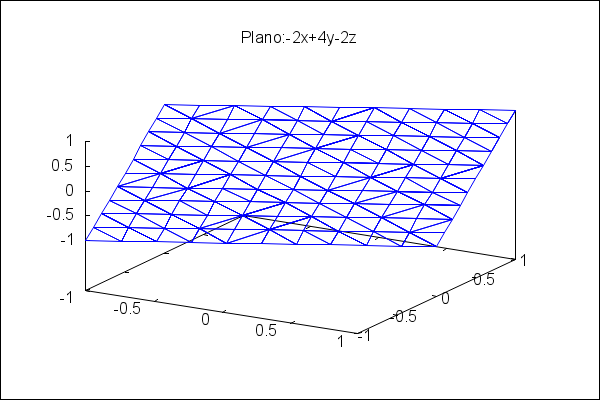
\includegraphics[height=2.6in,width=4.5in]{VOLUMEN_1/01_Vectores_Cartesianos/Figuras/Figura1_5aMax}
\end{center}
\end{figure}

\begin{center}
{\color{red}\rule{15.8cm}{0.4mm}}
\end{center}


\subsection{{\color{OliveGreen}Ejercicios}}
\label{EjerciciosAplicacionVectores}

\begin{enumerate}
\item Para las rectas dadas a continuaci�n: 
\begin{enumerate}
\item $L: \quad  \frac{3x-1}{4}= \frac{2y+3}{2}= {2-3z}$.
\item $L: \quad  \frac{2x+1}{3}= \frac{3y+2}{3}= -2+4z$.
\end{enumerate}
Encuentre los vectores posici�n para dos puntos diferentes sobre la recta y un vector unitario paralelo a la recta $L$.


\item Dada una linea recta $L_1$ que pasa a trav�s de los puntos $(-2,3,1)$ y $(1,4,6)$ encuentre:
\begin{enumerate}
\item El vector posici�n de un punto sobre la recta y un vector paralelo a �sta.
\item Una recta $L_2$ paralela a $L_1$ y que pase por el punto $(1,2,1)$.
\end{enumerate}

\item Una linea recta tiene como ecuaci�n vectorial: 
${\bf r}= {\bf a}+\lambda {\bf b}$, donde: ${\bf a}=3{\bf j}+2{\bf k}$ y ${\bf b}=2{\bf i}+ {\bf j}+2{\bf k}$. 

Encuentre la ecuaci�n cartesiana de la recta y las coordenadas de tres puntos sobre la recta.

\item Una linea recta pasa por el punto  $(3,2,-3)$ y paralela al vector ${\bf a}=2{\bf i}+3{\bf j}-3{\bf k}$. Encuentre la ecuaci�n cartesiana de la recta y las coordenadas de tres puntos sobre la recta.

\item Dado un plano que pasa por el punto $(2,3,-5)$ y con vector normal ${\bf a}=2{\bf i}+{\bf k}$, encuentre la forma cartesiana de la ecuaci�n del plano.

\item Encuentre la ecuaci�n del plano con normal ${\bf a}$ y que contiene el punto $P$ cuando:
\begin{enumerate}
\item ${\bf a}=2{\bf i}-3{\bf j}+{\bf k}$, $P=(1,0,1)$.
\item ${\bf a}={\bf i}-2{\bf j}+2{\bf k}$, $P=(2,-3,4)$.
\end{enumerate}


 \begin{figure}[t]
\begin{center}
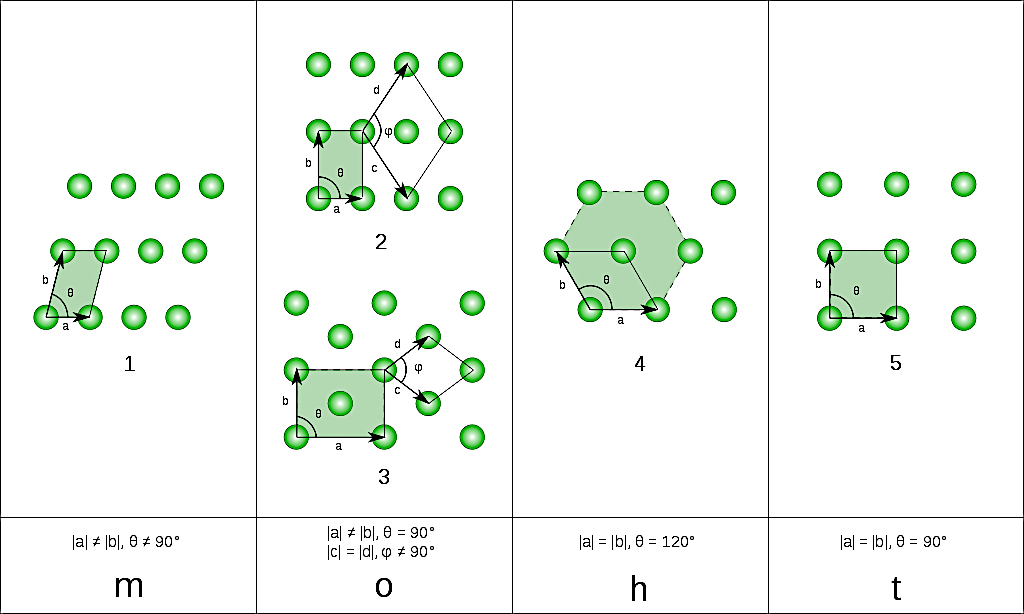
\includegraphics[width=4.5in]{VOLUMEN_1/01_Vectores_Cartesianos/Figuras/Figura1_6.jpg}
\caption{Las 5 redes de Bravais bidimensionales fundamentales:  1 Oblicuas, 2 rectangular, 3 rectangular centrada (r�mbica), 4 hexagonal, y 5 cuadrada. Figura tomada de \url{http://en.wikipedia.org/wiki/Bravais_lattice}.}
\label{fig6Capt1}
\end{center}
\end{figure}  

\item El �ngulo entre dos planos se define como el �ngulo entre sus normales. Encuentre el �ngulo entre los siguientes planos:
\begin{enumerate}
\item $x+3y+2z= 4$ y  $2x-5y+z=2$.
\item $3x+2y-2z=4$ y  $2x+y+2z=1$.
\end{enumerate}

\item Demuestre que la ecuaci�n de una esfera puede expresarse como: 
\[
|{\bf r}-{\bf c}|^2 = ({\bf r}-{\bf c}) \cdot ({\bf r}-{\bf c})= a^2\,,
\]
donde ${\bf c}$ es el vector posici�n del centro de la esfera y $a$ el radio.


\item Auguste Bravais\footnote{\url{http://en.wikipedia.org/wiki/Auguste_Bravais}} se dio cuenta que replicando un arreglo geom�trico muy simple, se puede describir una estructura cristalina. Dicho de otro modo, que conociendo una celda simple, podemos conocer la estructura cristalina. Esto es, que las posiciones de los �tomos en una red cristalina puede ser descrita por un vector: 
\[
{\bf R} = \mathbf{a} + \mathbf{b} + \mathbf{c} = n^{1}{\bf a}_{1} + n^{2}{\bf a}_{2} +n^{3}{\bf a}_{3} = n^{i}{\bf a}_{i} \,,
\] 
donde los ${\bf a}_{i}$ son vectores no coplanares (vectores primitivos o, simplemente en nuestro lenguaje, vectores base). Los $ n^{i}$ son n�meros enteros (negativos, cero o positivos). La posici�n de cada �tomo de un cristal puede ser descrita como reescalamientos (discretos) de este vector gen�rico o, de manera m�s precisa, la traslaci�n del origen de coordenadas por un vector.  

Ese concepto se conoce como redes de Bravais\footnote{\url{http://en.wikipedia.org/wiki/Bravais_lattice}}. En cada red puede haber varios vectores primitivos\footnote{\url{http://www.engr.sjsu.edu/rkwok/Phys175A/Chapter\%201.pdf}}. Se puede definir la \textit{celda primitiva} como la estructura m�nima que replicada reproduce todo el cristal. Vale decir, la estructura cristalina es invariante bajo traslaciones espaciales del tipo:
\[
{\bf{R}'} = {\bf R} + {\bf T}  \,, \quad \mbox{con } \,\, {\bf T} = m^{i}{\bf a}_{i} \,.
\]

\begin{figure}[t]
\begin{center}

\includegraphics[height=1.8in,width=2.0in]{VOLUMEN_1/01_Vectores_Cartesianos/Figuras/Figura1_7a.jpg}
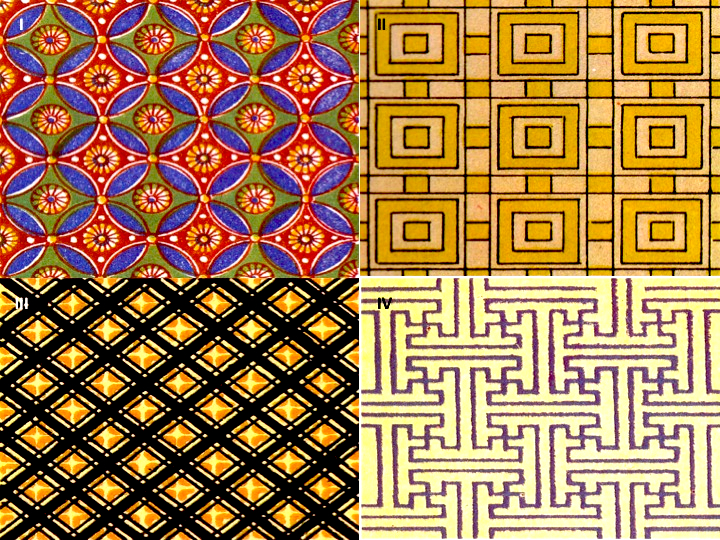
\includegraphics[height=1.8in,width=2.0in]{VOLUMEN_1/01_Vectores_Cartesianos/Figuras/Figura1_7b.jpg}
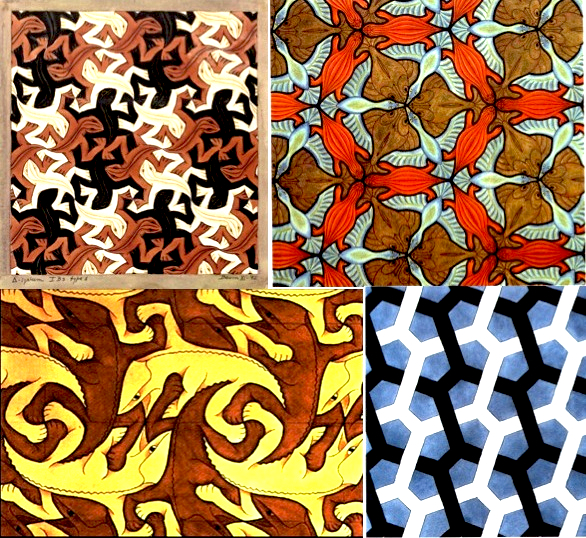
\includegraphics[height=1.8in,width=2.0in]{VOLUMEN_1/01_Vectores_Cartesianos/Figuras/Figura1_7c.jpg}
\caption{A la izquierda red cristalina bidimensional. Al centro cuatro detalles geom�tricos: mural egipcio, mural asirio, tejido tahit� e ilustraci�n en pieza de porcelana china (Tomado de: \url{http://en.wikipedia.org/wiki/Wallpaper_group}).  A la derecha, teselados de M.C. Escher, tomados de: \url{http://www.wikipaintings.org/en/paintings-by-genre/tessellation?firstArtist=m-c-escher\#artist-m-c-escher}.}
\label{fig7Capt1}
\end{center}
\end{figure} 

\begin{enumerate}
\item \textbf{Redes de Bravais bidimensionales}.  Tal y como muestra la figura \ref{fig6Capt1} existen 5 tipos distintos de redes de Bravais bidimensionales.

\begin{enumerate}
\item Dada la red bidimensional de la figura \ref{fig7Capt1} (Izquierda) encuentre todos los posibles vectores primitivos y celdas primitivas asociadas.

 \item La humanidad ha estado seducida por la geometr�a desde que empez� a representar figuras. A partir de las cuatro im�genes que se ilustran en la figura \ref{fig7Capt1} (Centro), encuentre todos los posibles vectores  y celdas primitivas asociadas.

\item Maurits Cornelis Escher\footnote{\url{http://en.wikipedia.org/wiki/M._C._Escher}} fue un fenomenal dibujante holand�s, quien se interes� por las simetr�as de los grupos de im�genes de papel tapiz. Berend, hermano de Maurits, era cristal�grafo y le mostr� la belleza de las simetr�as de la naturaleza. En las cuatro obras del g�nero de teselado\footnote{\url{http://en.wikipedia.org/wiki/Tessellation}}  de M.C. Escher, presentadas en la figura \ref{fig7Capt1} (Derecha) encuentre todos los posibles vectores  y celdas primitivas asociadas.
\end{enumerate}


\item \textbf{Redes de Bravais tridimensionales}. Este tipo de redes complica un poco m�s el escenario. Se puede demostrar que existen 14 de estas redes, tal y como se muestran en la figura \ref{fig8Capt1}.
 

\begin{enumerate}
 \item Muestre que los vol�menes de ocupaci�n at�mica, para los sistemas: monocl�nico, tricl�nico, ortor�mbico, tetragonal, rombo�drico, hexagonal y c�bico, corresponden a las expresiones que se muestran en la figura \ref{fig8Capt1}. 
 
\begin{figure}[t]
\begin{center}
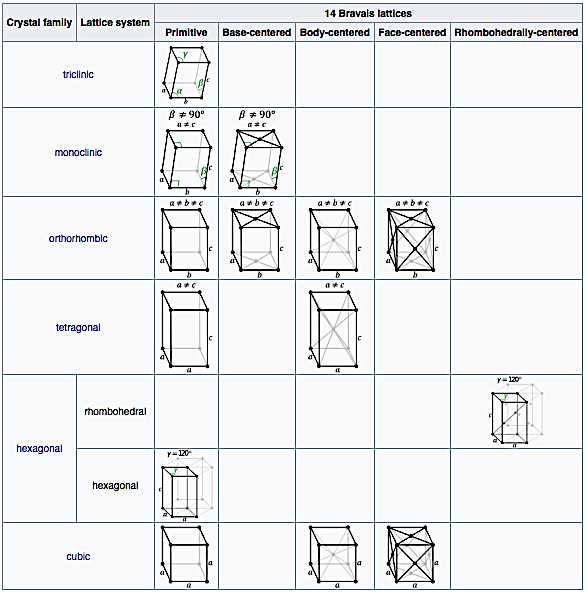
\includegraphics[width=4in]{VOLUMEN_1/01_Vectores_Cartesianos/Figuras/Figura1_8.jpg}
\caption{Las 14 Redes de Bravais tridimensionales y las estructuras cristalinas asociadas. Tomado de: \url{http://en.wikipedia.org/wiki/Bravais_lattice}.}
\label{fig8Capt1}
\end{center}
\end{figure}
\end{enumerate} 

\item El sistema c�bico, el m�s simple, corresponde a un sistema con un �nico par�metro de red $a= |\mathbf{a}|$, ya que  $ \mathbf{a} = \mathbf{b} = \mathbf{c} $. Adem�s, una posible descripci�n, para el caso m�s simple, es $ \mathbf{a} = {\bf i}\,,  \mathbf{b} = {\bf j}\,,   \mathbf{c} ={\bf k}$, los tres vectores cartesianos ortogonales. Existen otros sistemas que tambi�n est�n asociados al c�bico. Estos son el sistema c�bico cara centrada (\textit{fcc} por sus siglas en ingl�s) y c�bico cuerpo centrado (\textit{bcc}). En el primero existen �tomos en el centro de cada una de las caras del cubo definido por la tr�ada, $ \mathbf{a} = \mathbf{b} = \mathbf{c}$. En el sistema \textit{fcc} se a�ade un �tomo la centro del cubo simple. 

\begin{enumerate}
\item Muestre que un sistema \textit{bcc} tambi�n puede ser descrito por los vectores primitivos: 
\[
\mathbf{a} = a {\bf i}\,,\quad \mathbf{b} = a {\bf j} \,,\quad 
\mathbf{c} = a({\bf i} + {\bf j} +{\bf k})/2 \,.
\] 
Dibuje la celda primitiva y calcule su volumen.
\item Muestre que un sistema \textit{bcc} tambi�n puede ser descrito por los vectores primitivos: 
\[
\mathbf{a} = a ({\bf j} + {\bf k} -  {\bf i})/2\,,\quad 
\mathbf{b} = a ({\bf k} + {\bf i} -  {\bf j})/2\,,\quad
\mathbf{c} = a( {\bf i} + {\bf j} -{\bf k})/2\,.
\] 
Dibuje la celda primitiva y calcule su volumen.
\item Muestre que un sistema \textit{fcc} tambi�n puede ser descrito por los vectores primitivos: 
\[
\mathbf{a} =  a( {\bf j} +{\bf k})/2\,,\quad
\mathbf{b}  = a( {\bf i} + {\bf k})/2\,,\quad
\mathbf{c} =  a( {\bf i} + {\bf j})/2 \,.
\] 
Otra vez, dibuje la celda primitiva y calcule su volumen.
\end{enumerate}

\item Se puede definir la red rec�proca como:
 \[
 \mathbf{a'} = \frac{\mathbf{b} \times \mathbf{c} }{ \mathbf{a} \cdot (\mathbf{b} \times \mathbf{c} )}\,,\quad
  \mathbf{b'} = \frac{\mathbf{c} \times \mathbf{a} }{ \mathbf{a} \cdot (\mathbf{b} \times \mathbf{c} )} \quad \mbox{y} \quad 
  \mathbf{c'} = \frac{\mathbf{a} \times \mathbf{b} }{ \mathbf{a} \cdot (\mathbf{b} \times \mathbf{c} )} \,.
 \] 
 De esta manera es claro que, por construcci�n, $ \mathbf{a'} \cdot \mathbf{b} = \mathbf{a'} \cdot \mathbf{c}  = 0$ y adem�s $\mathbf{a'} \cdot \mathbf{a} = 1$. Con lo cual podemos generalizarlo como $ \mathbf{\hat{e}}^{i'} \cdot \mathbf{\hat{e}}_{j} = \delta^{i'}_{j}$. 
 
 Exprese los vectores y las celdas rec�procas para los  sistemas c�bico simple, y los distintos \textit{bcc} y \textit{fcc}. Calcule adem�s el volumen de cada celda rec�proca. 
 
\end{enumerate}
\item Realice los c�lculos anteriores utilizando el programa {\bf Maxima}.

\end{enumerate}


\section{�lgebra vectorial con �ndices}
\label{AlgebraVectorialIndices}
\index{Algebra vectorial con �ndices}
Antes de comenzar con la presentaci�n de este esquema de c�lculo cabe aclarar algunas costumbres y convenciones con la notaci�n de �ndices que estaremos utilizando durante el resto de este curso.
\subsection{Convenci�n de Einstein}
\label{ConvencionEinstein}
\index{Einstein!Convenci�n de}
\index{Convenci�n de Einstein}
\index{�ndices!Convenci�n de Einstein}

El convenio de suma de Einstein, es una simplificaci�n que se utiliza para abreviar la escritura de las sumatorias, en el que se suprime el s�mbolo de sumatoria y consiste en lo siguiente:

\begin{enumerate}
\item  Los �ndices repetidos (arriba y abajo) indicar�n suma por los valores que tomen los �ndices. Las componentes de los vectores tendr�n �ndices arriba y los vectores base abajo:
\[
{\bf a}=a^{1}\mathbf{e}_{1}+a^{2}\mathbf{e}_{2}+a^{3}\mathbf{e}_{3}=
\sum_{m=1}^{3}a^{m}\mathbf{e}_{m}\quad\Leftrightarrow\quad{\bf a}=
a^{m}\mathbf{e}_{m} = a^{i}\mathbf{e}_{i} \,.
\]

\item  Los �ndices repetidos son mudos (no importa las letras que los etiquete) y representan suma. As�:
\[
{k}^{j}{a}_{j}={k}^{m}{a}_{m}={k}^{1}{a}_{1} +{k}^{2}{a}_{2} +{k}^{3}{a}_{3}={b} \,.
\]

En este punto del discurso, la posici�n de los �ndices (arriba y abajo) solo tiene sentido est�tico y solo as� indican suma. 
M�s adelante veremos que representan cantidades distintas.
\item  Llamaremos contracci�n cuando sumamos respecto a un par de �ndices, vale decir:
\[
{A}_{i}^{j} \,\, \Rightarrow \,\, 
\sum_{i}{A}_{i}^{i}={A}_{1}^{1}+{A}_{2}^{2} +{A}_{3}^{3} 
\,\, \Rightarrow \,\,
{A}_{i}^{i}={A}_{1}^{1}+{A}_{2}^{2}+{A}_{3}^{3} \,.
\]
\end{enumerate}

Las cantidades con dos o m�s �ndices las llamaremos componentes de tensores, y deben entenderse como arreglos bidimensionales (tridimensionales, tetradimensionales, seg�n el n�mero de �ndices). Estas cantidades ser�n considerados en detalle posteriormente pero  por ahora, content�monos con saber qu� cosas son cantidades con dos �ndices. Es claro que la contracci�n de �ndices convierte un conjunto de n�meros $\left(  i \times j \right) \rightarrow 1$, en un s�lo n�mero. 

Los �ndices libres (aquellos que no est�n sumados) indican el n�mero de objetos disponibles y deben mantenerse a ambos lados de la ecuaci�n. Por ejemplo:
\[
{B}_{i}= {K}_{i}^{k}{A}_{k} \quad\Leftrightarrow\quad
\left\{
\begin{array}
[c]{c}
{K}_{1}^{1}{A}_{1}+{K}_{1}^{2}{A}_{2}+{K}_{1}^{3}{A}_{3}={B}_{1}\\
\\
{K}_{2}^{1}{A}_{1}+{K}_{2}^{2}{A}_{2}+{K}_{2}^{3}{A}_{3}={B}_{2}\\
\\
{K}_{3}^{1}{A}_{1}+{K}_{3}^{2}{A}_{2}+{K}_{3}^{3}{A}_{3}={B}_{1}
\end{array}
\right.
\]
con lo cual ${B}_{i}={K}_{i}^{k}{A}_{k}$ representa 3 ecuaciones. La operaci�n ${B}_{ij}={K}_{i}^{k}{A}_{kj}$ representa 9.


\index{Kronecker!Delta de}
\index{Delta de Kronecker}
\index{Kronecker!Leopold Kronecker}
La delta de Kronecker\footnote{Leopold Kronecker (7 diciembre 1823 Legnica, Polonia, 29 diciembre 1891, Berlin, Alemania) Matem�tico polaco con importantes contribuciones en teor�a de n�meros, funciones el�pticas y �lgebra, as� como la interrelaci�n entre estas disciplinas.} es un objeto matem�tico de dos �ndices, representa $\delta_{i}^{k}=1$ si $i=k$, y es nula en los otros casos. Por ejemplo:
\[
{K}_{ij}^{k}\ \delta_{k}^{i}={K}_{1j}^{1}\underset{=1}{\underbrace{\delta_{1}^{1}}}+{K}_{2j}^{1}\overset{=0}
{\overbrace{\delta_{1}^{2}}}+{K}_{3j}^{1}\overset{=0}{\overbrace
{\delta_{1}^{3}}}+{K}_{1j}^{2}\overset{=0}{\overbrace{\delta_{2}^{1}}
}+{K}_{2j}^{2}\underset{=1}{\underbrace{\delta_{2}^{2}}}+{K}
_{3j}^{2}\overset{=0}{\overbrace{\delta_{2}^{3}}}+{K}_{1j}^{3}
\overset{=0}{\overbrace{\delta_{3}^{1}}}+{K}_{2j}^{3}\overset
{=0}{\overbrace{\delta_{3}^{2}}}+{K}_{3j}^{3}\ \underset{=1}
{\underbrace{\delta_{3}^{3}}}\,,
\]
es decir:
\[
{K}_{ij}^{k}\ \delta_{k}^{i}={K}_{kj}^{k}={K}_{ij}^{i}={K}_{1j}^{1}+{K}_{2j}^{2}+{K}_{3j}^{3} \,.
\]
\index{Levi-Civita!Tensor}
\index{Tensor!Levi-Civita} 
\index{Levi-Civita!Tullio Levi-Civita}

Adem�s de la delta de Kronecker introduciremos el s�mbolo de permutaci�n de Levi-Civita\footnote{Tullio Levi-Civita (1873 Padova, Veneto, 1941 Roma, Italia) Ge�metra italiano y uno de los desarrolladores del c�lculo tensorial que m�s tarde ser�a utilizado por Einstein y Weyl como el lenguaje de la Relatividad General.}, $\varepsilon^{ijk}$, para el caso de tres dimensiones: $i,j,k=1,2,3$.
\[
\varepsilon_{ijk}=\varepsilon^{ijk}=\left\{
\begin{array}
[c]{ll}
+1 & \mbox{cuando}\quad \{\left(i,j,k\right)=\left(1,2,3\right) ;\left(  3,1,2\right)
;\left(  2,3,1\right)  \}\mbox{ permutaci�n c�clica}\\
-1 & \mbox{cuando}\quad \{\left(i,j,k\right)=\left(  1,3,2\right)  ;\left(  3,2,1\right)
;\left(  2,1,3\right)  \}\mbox{ permutaci�n impar o antic�clica}\\
\ \ 0 & \mbox{cuando}\quad  \{i=j\,,\quad  i=k\quad \wedge\quad  j=k\} 
\end{array}
\right.
\]
Por lo tanto, es distinto de cero cuando todos los �ndices son diferentes. Toma el valor $1$ si la permutaci�n de �ndices es c�clica (o par), y toma el valor $-1$ si la permutaci�n es antic�clica (o impar). 

Si queremos calcular, por ejemplo:  $c^{i}=\varepsilon^{ijk}a_{j}b_{k}$, entonces resulta:
\begin{eqnarray*}
c^{1}=\varepsilon^{111}a_{1}b_{1}+\varepsilon^{112}a_{1}b_{2}+\varepsilon^{113} a_{1}b_{3}+\varepsilon^{121}a_{2}b_{1}+\varepsilon^{122}a_{2}b_{2}+\varepsilon^{123}a_{2}b_{3}+\varepsilon^{131}a_{3}b_{1}+\varepsilon^{132}a_{3}b_{2}+\varepsilon^{133}a_{3}b_{3}\,, \\
c^{2}=\varepsilon^{211}a_{1}b_{1}+\varepsilon^{212}a_{1}b_{2}+\varepsilon^{213}a_{1}b_{3}+\varepsilon^{221}a_{2}b_{1}+\varepsilon^{222}a_{2}b_{2}+\varepsilon^{223}a_{2}b_{3}+\varepsilon^{231}a_{3}b_{1}+\varepsilon^{232}a_{3}b_{2}+\varepsilon^{233}a_{3}b_{3} \,,\\
c^{3}=\varepsilon^{311}a_{1}b_{1}+\varepsilon^{312}a_{1}b_{2}+\varepsilon^{313}a_{1}b_{3}+\varepsilon^{321}a_{2}b_{1}+\varepsilon^{322}a_{2}b_{2}+\varepsilon^{323}a_{2}b_{3}+\varepsilon^{331}a_{3}b_{1}+\varepsilon^{332}a_{3}b_{2}+\varepsilon^{333}a_{3}b_{3} \,,
\end{eqnarray*}
con lo cual:
\[
c^{i}=\varepsilon^{ijk}a_{j}b_{k}\,\, \Rightarrow \,\, \left\{
\begin{array}
[c]{c}
c^{1}=\varepsilon^{123}a_{2}b_{3}+\varepsilon^{132}a_{3}b_{2}=a_{2}b_{3}-a_{3}b_{2}\\
\\
c^{2}=\varepsilon^{231}a_{3}b_{1}+\varepsilon^{213}a_{1}b_{3}=a_{3}b_{1}-a_{1}b_{3}\\
\\
c^{3}=\varepsilon^{312}a_{1}b_{2}+\varepsilon^{321}a_{2}b_{1}=a_{1}b_{2}-a_{2}b_{1}
\end{array}
\right.
\]

A continuaci�n enumeramos algunas propiedades de la delta de Kronecker y del s�mbolo de permutaci�n de Levi-Civita, dejamos al lector su demostraci�n. Ellas son:
\begin{align*}
\delta_{j}^{j}  &  =3 \,,\\
\varepsilon_{jkm}\varepsilon^{ilm}  &  =\delta_{j}^{i}\delta_{k}^{l}
-\delta_{k}^{i}\delta_{j}^{l}=\delta_{j}^{i}\delta_{k}^{l}-\delta_{j}
^{l}\delta_{k}^{i} \,, \\
\varepsilon_{jmn}\varepsilon^{imn}  &  =2\delta_{j}^{i}\,,\\
\varepsilon_{ijk}\varepsilon^{ijk}  &  =6 \,.
\end{align*}


\subsection{Vectores e �ndices}
\index{�ndices!�lgebra de vectores}
\index{Vectores 3D!�lgebra con �ndices}

Disponemos ahora de una manera m�s elegante para escribir ecuaciones que involucren vectores. Veamos que forma toma el �lgebra vectorial con esta nueva notaci�n.

\subsubsection{Sumas de vectores}
La suma de vectores ser� expresada de la siguiente manera:
\[
{\bf a}+{\bf b}=a^{i}\mathbf{e}_{i}+b^{i}\mathbf{e}_{i}=\left(  a^{i}+b^{i}\right)  \mathbf{e}_{i}=c^{i} \mathbf{e}_{i}\,\, \Rightarrow \,\,  c^{i}=a^{i}+b^{i}\quad\text{con }i=1,2,3 \,.
\]

\subsubsection{Producto escalar}
A partir da ahora y de forma equivalente, expresaremos el producto escalar en t�rmino de los �ndices. De forma y manera que:
\[
{\bf a}\cdot{\bf b}=\left|  {\bf a}\right|  \left|  {\bf b}\right| \cos(\theta)_{{\bf a}{\bf b}}=a^{i}b_{i} \quad \text{con }i=1,2,3 \,.
\]

\subsubsection{Producto vectorial}
En t�rminos de �ndices, la componente $i$ del producto vectorial se puede expresar como:
\[
{c}^i=\left({\bf a}\times{\bf b}\right) ^{i}=\varepsilon^{ijk} a_{j}  b_{k} \quad \text{con }i,j,k=1,2,3 \,.
\]
De esta manera, todas las particularidades de producto vectorial ahora descansan en las propiedades del s�mbolo de Levi-Civita.

\subsubsection{Triple producto mixto}
Para finalizar, analicemos ahora el n�mero (pseudoescalar) que proviene de la multiplicaci�n mixta:
\[
{\bf c}\cdot\left(  {\bf a}\times{\bf b}\right)  =\left|  {\bf c}\right| \left|   {\bf a}\times{\bf b}  \right|  \cos(\theta)
_{\left\langle {\bf c},{\bf a}\times{\bf b}\right\rangle }=c^{i}
 \varepsilon_{ijk}\ a^{j}b^{k}= \varepsilon_{ijk}\ c^{i} a^{j}b^{k}  =  \left|
\begin{array}
[c]{ccc}
 c^1 &  c^2 &  c^3\\
a^1 & a^2 & a^3\\
 b^1 &  b^2 &  b^3
\end{array}
\right| \,.
\]

\subsection{Rotaci�n de coordenadas}
\label{RotacionCoordenadas}
\index{Rotaci�n de coordenadas}
\index{Coordenadas! Rotaci�n de}
Consideremos un sistema de coordenadas cartesiano $(x,y,z)$ y su base can�nica $\{{\bf i}, {\bf j}, {\bf k}\}$, si rotamos el sistema de coordenadas un �ngulo $\phi$ alrededor del eje $z$ tendremos un nuevo sistema de coordenadas $({\tilde x}, {\tilde y}, {\tilde z})$ y una nueva base $\{\tilde{\bf i}, \tilde{\bf j}, \tilde{\bf k}\}$. La regla de transformaci�n que relaciona ambos sistemas de coordenadas es:
\[
\left\{
\begin{array}
[c]{ccl}
x & = & {\tilde x}\cos(\phi)- {\tilde y}\ \mbox{sen}(\phi)\\
y & = & {\tilde x}\ \mbox{sen}(\phi)+ {\tilde y}\cos(\phi) \\
z & = & {\tilde z}
\end{array}
\right.   \quad  \Longleftrightarrow \quad 
\left\{
\begin{array}
[c]{ccl}
{\tilde x} & = & { x}\cos(\phi) + { y}\ \mbox{sen}(\phi)\\
{\tilde y} & = & -{ x}\ \mbox{sen}(\phi)+ { y}\cos(\phi) \\
{\tilde z}& = & { z}
\end{array}
\right.
\label{rotacionejez}
\]

Mientras que las bases transformar�n, como veremos m�s adelante, como:
\[
\left\{
\begin{array}
[c]{ccl}
\tilde{\bf i} & = & {\bf i}\cos(\phi)+{\bf j}\ \mbox{sen}(\phi)\\
\tilde{\bf j} & = & -{\bf i}\ \mbox{sen}(\phi)+ {\bf j}\cos(\phi) \\
\tilde{\bf k} & = & {\bf k}
\end{array}
\right. 
\]

Diremos que un triplete de n�meros $\left(a^1, a^2,  a^3\right)$ definen las componente de un vector ${\bf a}=a^1{\bf i}+a^2{\bf j}+a^3{\bf k}$ si estas cantidades transforman bajo rotaci�n de la siguiente manera:
\[
{\tilde a}_1  =  {a}_1\cos(\phi) + {a}_2\ \mbox{sen}(\phi)\,, \quad \,
{\tilde a}_2  =  -{a}_1\ \mbox{sen}(\phi)+ {a}_2\cos(\phi) \,, \quad \,
{\tilde a}_3  =  {a}_3 \, .
\]

Notemos tambi�n lo siguiente, al usar la notaci�n de �ndices podemos escribir las ecuaciones de transformaci�n de coordenadas as�:
\[
\left\{
\begin{array}
[c]{ccl}
{\tilde x} & = & { x}\cos(\phi) + { y}\ \mbox{sen}(\phi)\\
{\tilde y} & = & -{ x}\ \mbox{sen}(\phi)+ { y}\cos(\phi) \\
{\tilde z}& = & { z}
\end{array} 
\right. \,\,  \Rightarrow \,\, 
\left\{
\begin{array}
[c]{ccl}
{\tilde x}^1&=& A^1_1 {x}^1+A^1_2{x}^2+A^1_3{x}^3\\
{\tilde x}^2&=& A^2_1 {x}^1+A^2_2{x}^2+A^2_3{x}^3\\
{\tilde x}^3&=& A^3_1 {x}^1+A^3_2{x}^2+A^3_3{x}^3
\end{array} 
\right.
\,\,  \Rightarrow \,\,
{\tilde x}^i= {\tilde A}^i_j {x}^j \,, 
\label{transrota}
\]
con: $i,j=1, 2, 3$. 

Se puede ver f�cilmente que las cantidades ${\tilde A}^i_j$, en coordenadas cartesianas, vienen dadas por:
\[
{\tilde A}^i_j  =\frac{\partial {\tilde x}^i}{\partial x^j} \,,
\]
y como la transformaci�n de coordenadas es invertible, se tiene que:
\[
x^j= A^j_i {\tilde x}^i \,, \quad \, \mbox{con:}\quad \, A^j_i  =\frac{\partial {x}^j}{\partial {\tilde x}^i}\,,
\]
y se cumple la siguiente condici�n de ortogonalidad:
\[
{\tilde A}^i_k A^j_i =\delta^j_k\,.
\]
Por lo tanto, en general, diremos que las componentes de un vector transformar�n de la manera siguiente:
\[
\label{transformacomponentes1}
{\tilde a}^i =\frac{\partial {\tilde x}^i}{\partial x^j} {a}^j \equiv  {\tilde A}^i_j {a}^j\,\quad \Leftrightarrow \quad
a^i = \frac{\partial  x^i}{\partial {\tilde x}^j} {a}^j \equiv   A^i_j {a}^j\ \,.
\]


\subsection{Escalares, pseudoescalares, vectores y pseudovectores}
\label{PseudoCantidades}
\index{Pseudo-escalares}
\index{Pseudo-vectores}
Adem�s de las rotaciones podemos considerar otra clase de transformaciones: las reflexiones. Estas transformaciones, $(x^{1}, x^{2}, x^{3}) \rightarrow (-x^{1}, x^{2}, x^{3})$, muestran una sutil diferencia entre dos tipos de cantidades vectoriales: los vectores polares y los axiales, diferencia que no se puede apreciar en las rotaciones.

Una reflexi�n en el plano $yz$ se puede representar como un cambio de signo en la componente $x$ del vector: 
\begin{equation}
(a_{x}, a_{y}, a_{z})  \rightarrow (-a_{x}, a_{y}, a_{z}) \,,
\label{reflexion}
\end{equation}
o tambi�n:
\[
a^{1}\mathbf{e}_{1} + a^{2}\mathbf{e}_{2} +a^{3}\mathbf{e}_{3} \rightarrow  
a^{1}(-\mathbf{e}_{1}) + a^{2}\mathbf{e}_{2} +a^{3}\mathbf{e}_{3} \equiv 
(-a^{1})\mathbf{e}_{1} + a^{2}\mathbf{e}_{2} +a^{3}\mathbf{e}_{3} \, .
\]

Diremos que los objetos que transforman de esta manera bajo reflexi�n son vectores polares o simplemente vectores. N�tese que esa transformaci�n de coordenadas es equivalente a invertir el vector base: $\mathbf{e}_{1} \rightarrow -\mathbf{e}_{1}$. 

Ahora bien, si dos vectores polares $\mathbf{a}$ y $\mathbf{b}$, son transformados bajo reflexi�n como en (\ref{reflexion}), entonces un vector axial $\mathbf{c}$ transformar� como: 
\[
\mathbf{c} = \mathbf{a} \times \mathbf{b} \rightarrow  \mathbf{\tilde{a}} \times \mathbf{\tilde{b}} = -\mathbf{\tilde{c}}\,. 
\]
Es decir, los vectores axiales o pseudovectores cambian de signo bajo reflexi�n de los vectores que los generan\footnote{Esta inversi�n de vector axial puede comprobarse f�cilmente utilizando la definici�n de productor vectorial (\ref{produtovectorial1}) en la cual se aprecia que un cambio en el signo en $a_{x}$ y $b_{x}$ induce un cambio de signo en $c_{y}$ y $c_{z}$.}. 

De igual manera notamos que $d ={\bf a} \cdot {\bf b}$ queda invariante bajo la transformaci�n (\ref{reflexion}), mientras que $V={\bf c}\cdot\left(  {\bf a}\times{\bf b}\right)$ cambia de signo. Siguiendo el ejemplo de vectores y pseudovectores, llamaremos escalar a $d$ y pseudoescalar a $V$. 

Existen importantes cantidades f�sicas que vienen representadas por pseudovectores, entre ellas mencionamos: la cantidad de momento angular, $ \mathbf{L} = \mathbf{r} \times \mathbf{p}$; el torque ${\boldsymbol \tau} =\mathbf{r} \times \mathbf{F}$  y el campo de inducci�n magn�tica, 
$\dfrac{\partial \mathbf{B}}{\partial t}=- \mathbf{\nabla} \times\mathbf{E}$. 

Pseudovectores y vectores representan distintos objetos geom�tricos. Los primeros se asocian a orientaciones de superficies, mientras que los segundos lo est�n con segmentos de rectas orientadas. El vector velocidad angular, ${\boldsymbol \omega}$, es un pseudovector por cuanto $\mathbf{r}$ y $\mathbf{v}$ son vectores polares y $\mathbf{v} = {\boldsymbol  \omega } \times \mathbf{r}$.  Algo equivalente ocurre con la aceleraci�n de Lorentz $\mathbf{a} = q\mathbf{v}\times \mathbf{B}$, donde $\mathbf{B}$ es el campo magn�tico.  

En general, podemos representar la reflexi�n (\ref{reflexion}) bajo el esquema que presentamos en (\ref{transformacomponentes1}), es decir, como transformaciones del tipo: 
\[
\left(
\begin{array}{r}
\tilde{a}_{x} \\        
\tilde{a}_{y} \\
\tilde{a}_{z} \\        
\end{array}
\right) \equiv
\left(
\begin{array}{r}
-a_{x} \\        
a_{y} \\
a_{z} \\        
\end{array}
\right) =
\left(
\begin{array}{rrr}
-1 & 0 & 0 \\        
 0 & 1 & 0 \\
 0 &  0 & 1\\        
\end{array}
\right) 
\left(
\begin{array}{c}
a_{x} \\        
a_{y} \\
a_{z} \\        
\end{array}
\right) \,.
\]
donde:
\[
 {\tilde a}^i = {\tilde A}^i_j {a}^j \, , 
\,\, \text{donde} \,\,\,
{\tilde A}^i_j = \frac{\partial {\tilde x}^i}{\partial x^j} =
\left(
\begin{array}{rrr}
-1 & 0 & 0 \\        
 0 & 1 & 0 \\
 0 &  0 & 1\\        
\end{array}
\right) \,,
\]
es la matriz de transformaci�n de coordenadas\footnote{Una discusi�n de vectores y pseudovectores puede consultarse en la nota de Quigley, Robert J. ``Pseudovectors and Reflections'' American Journal of Physics 41, no. 3 (1973): 428-430; y en el cap�tulo 52 del Vol. 1 de Feynman, R.P., Leighton, R.B. and Sands, M., 2013. The Feynman Lectures on Physics, Desktop Edition. Basic Books. Para algunas de las consecuencias que se presentan cuando se consideran cantidades f�sicas y transformaciones de reflexi�n.}. 

Notemos que aqu� el determinante de la matriz de transformaci�n tiene como valor $-1$ ($\det|{\tilde A}|=-1$) �Cu�l es el valor del determinante de la matriz que podemos asociar a (\ref{transrota})?

El hecho de que el $\det|{\tilde A}|=1$  o $\det|{\tilde A}|=-1$, permite clasificar a las transformaciones de coordenadas en {\it transformaciones propias} o {\it transformaciones impropias}, respectivamente. 

Entonces, en general, diremos que las componentes de vectores y pseudovectores transformar�n bajo reflexi�n de la siguiente manera:
\[
\text{si:} \quad {\tilde A}^i_j = \frac{\partial {\tilde x}^i}{\partial x^j}  \,\, \Rightarrow \,\,
\left\{
\begin{array}{ll}
{\tilde a}^i = {\tilde A}^i_j {a}^j \,,   &  \text{vectores polares o simplemente vectores, }  \\ \\
{\tilde p}^i = \det|{\tilde A}| {\tilde A}^i_j {p}^j   \,, &  \text{pseudovectores o vectores axiales}.      
\end{array}
\right.
\]
\newpage

\subsection{{\color{Fuchsia}Ejemplos}}
\label{ParCalculos}
\index{Ejemplos c�lculos vectoriales con �ndices}
\index{�ndices!Ejemplos c�lculos vectoriales}

\begin{enumerate}
\item Mostraremos a continuaci�n dos casos de identidades vectoriales que pueden ser f�cilmente demostradas mediante la utilizaci�n de �ndices.

\begin{enumerate}
\item ${\bf a}\times\left(  {\bf b}\times{\bf c}\right)  =\left(  {\bf c}
\cdot{\bf a}\right)  {\bf b}-\left(  {\bf a}\cdot{\bf b}\right)  {\bf c}$

El resultado ser� un vector, por lo tanto:
\begin{eqnarray*}
\left( {\bf a}\times\left(  {\bf b}\times{\bf c}\right)  \right)^{i}  
=\varepsilon^{ijk}a_{j}\left(  {\bf b}\times{\bf c}\right)_{k}
&=&\varepsilon^{ijk}a_{j}\varepsilon_{kmn}b^{m}c^{n}=\varepsilon
^{ijk}\varepsilon_{kmn}a_{j}b^{m}c^{n}=\varepsilon^{ijk}\varepsilon_{mnk}  a_{j}b^{m}c^{n}\\
&=& \left(  \delta_{m}^{i}\delta_{n}^{j}-\delta_{m}^{j}\delta_{n}^{i}\right)
a_{j}b^{m}c^{n}=\delta_{m}^{i}\delta_{n}^{j}a_{j}b^{m}c^{n}-\delta_{m}
^{j}\delta_{n}^{i}a_{j}b^{m}c^{n} \\
&=& \delta_{m}^{i}b^{m}\delta_{n}^{j}a_{j}c^{n}-\delta_{n}^{i}c^{n}\delta
_{m}^{j}a_{j}b^{m}=b^{i}\underset{\left(  {\bf c}\cdot{\bf a}\right)
}{\underbrace{a_{n}c^{n}}}-c^{i}\underset{\left(  {\bf a}\cdot{\bf b}\right)
}{\underbrace{a_{j}b^{j}}}\\
&=& b^{i}\left(  {\bf c}\cdot{\bf a}\right)  -c^{i}\left(  {\bf a}\cdot {\bf b} \right)= {\bf b} \left(  {\bf c}
\cdot{\bf a}\right) -{\bf c}\left(  {\bf a}\cdot{\bf b}\right) \,.
\end{eqnarray*}

En la segunda l�nea hemos hecho uso de la identidad: $\varepsilon_{jkm}\varepsilon^{ilm}   =\delta_{j}^{i}\delta_{k}^{l}
-\delta_{k}^{i}\delta_{j}^{l}=\delta_{j}^{i}\delta_{k}^{l}-\delta_{j}
^{l}\delta_{k}^{i} $.


\item $\left(  {\bf a}\times{\bf b}\right)  \cdot\left(  {\bf c}\times {\bf d} \right)  =
\left(  {\bf a}\cdot{\bf c}\right)  \left(  {\bf b}\cdot {\bf d} \right)  -
\left(  {\bf a}\cdot {\bf d} \right)  \left(  {\bf b}\cdot {\bf c} \right)  $

El lado derecho es un escalar, por lo tanto:
\begin{align*}
\left(  {\bf a}\times{\bf b}\right)  \cdot\left(  {\bf c}\times {\bf d} \right)   &  =
\left(  {\bf a}\times{\bf b}\right)  ^{l}\left(  {\bf c} \times {\bf d} \right)  _{l}\\
&  =\varepsilon^{ljk}a_{j}b_{k}\ \varepsilon_{lmn}c^{m}d^{n}=\varepsilon
^{ljk}\varepsilon_{lmn}\ a_{j}b_{k}c^{m}d^{n}\\
&  =\varepsilon^{jkl}\varepsilon_{mnl}\ a_{j}b_{k}c^{m}d^{n}=\left(
\delta_{m}^{j}\delta_{n}^{k}-\delta_{m}^{k}\delta_{n}^{j}\right)  a_{j}
b_{k}c^{m}d^{n}\\
&  =\delta_{m}^{j}\delta_{n}^{k}a_{j}b_{k}c^{m}d^{n}-\delta_{m}^{k}\delta
_{n}^{j}a_{j}b_{k}c^{m}d^{n}\\
&  =\underset{\left(  {\bf a}\cdot{\bf c}\right)  }{\underbrace{\delta_{m}
^{j}a_{j}c^{m}}}\underset{\left(  {\bf b}\cdot {\bf d} \right)  }{\underbrace
{\delta_{n}^{k}b_{k}d^{n}}}-\underset{\left(  {\bf b}\cdot{\bf c}\right)}
{\underbrace{\delta_{m}^{k}b_{k}c^{m}}}\underset{\left(  {\bf a}\cdot {\bf d} \right) }
{\underbrace{\delta_{n}^{j}a_{j}d^{n}}}\\
&  =\left(  {\bf a}\cdot{\bf c}\right)  \left(  {\bf b}\cdot {\bf d} \right)
-\left(  {\bf b}\cdot{\bf c}\right) \left(  {\bf a}\cdot {\bf d} \right)  \,.
\end{align*}\end{enumerate}

\item Si tenemos tres vectores $\{ {\bf a}, {\bf b}, {\bf c} \}$ queremos ver si se cumple: 
\[
 {\bf a} \times ({\bf b} \times {\bf c}) +  {\bf b} \times ({\bf c} \times {\bf a}) +  {\bf c} \times ({\bf a} \times {\bf b})= {\bf 0}\,.
 \] 

En notaci�n de �ndices resulta:
 \[
{\bf a} \times ({\bf b} \times {\bf c}) +  {\bf b} \times ({\bf c} \times {\bf a}) +  {\bf c} \times ({\bf a} \times {\bf b})    = 
  \epsilon^{lmi}a_{m}\epsilon_{ijk}b^{j}c^{k} + \epsilon^{lmi}b_{m}\epsilon_{ijk}c^{j}a^{k} + \epsilon^{lmi}c_{m}\epsilon_{ijk}a^{j}b^{k} \,,
 \]
con lo cual, arreglando:
\begin{eqnarray*}
\epsilon^{lmi}\epsilon_{ijk}a_{m}b^{j}c^{k} + \epsilon^{lmi}\epsilon_{ijk}b_{m}c^{j}a^{k} + \epsilon^{lmi}\epsilon_{ijk}c_{m}a^{j}b^{k} &=&
\left( \delta^{l}_{j} \delta^{m}_{k} -  \delta^{m}_{j} \delta^{l}_{k}  \right) a_{m}b^{j}c^{k} + \left( \delta^{l}_{j} \delta^{m}_{k} -  \delta^{m}_{j} \delta^{l}_{k}  \right) b_{m}c^{j}a^{k} \\
&+& 
 \left( \delta^{l}_{j} \delta^{m}_{k} -  \delta^{m}_{j} \delta^{l}_{k}  \right) c_{m}a^{j}b^{k} \,,
\end{eqnarray*}
y ahora desarrollando los productos de las $\delta$'s, e identificando t�rmino a t�rmino, notamos que se anulan:
\[
\underbrace{a_{k}b^{l}c^{k} }_{I}-\underbrace{a_{k}b^{k}c^{l} }_{II}+\underbrace{b_{k}c^{l}a^{k}}_{II}-\underbrace{b_{k}c^{k}a^{l}}_{III} 
+\underbrace{c_{k}a^{l}b^{k}}_{III}-\underbrace{c_{k}a^{k}b^{l}}_{I}  = 0\,.
 \]
 
\item Vimos que los vectores polares transforman bajo una reflexi�n respecto al plano $yz$ de la forma:
\[
{\bf e}_1 \rightarrow - {\bf e}_1 \,\, \Rightarrow \,\,
({\tilde a}^1,{\tilde a}^2,{\tilde a}^3)=(-{a}^1,{a}^2,{a}^3)\,.
\]

Para saber que pasa con el vector ${\bf c}={\bf a}\times {\bf b}$, cuando lo sometemos a esta reflexi�n, estudiemos como se transforman sus componentes directamente de la definici�n del producto vectorial, miremos con respecto a la componente $x$ de ${\bf c}$. Entonces, para ${\bf a}$ y ${\bf b}$ vectores polares se tiene:
\begin{eqnarray*}
\tilde{\bf c}=\tilde{\bf a}\times \tilde{\bf b}&=& \left[
\left( \tilde{a}^2 \tilde{b}^3-\tilde{a}^3 \tilde{b}^2\right) \,,
\left(\tilde{a}^3 \tilde{b}^1-\tilde{a}^1 \tilde{b}^3\right) \,,
\left(\tilde{a}^1 \tilde{b}^2-\tilde{a}^2 \tilde{b}^1\right) \right] \\
&=&\left[
\left( {a}^2 {b}^3-{a}^3 {b}^2\right)\,,
\left({a}^3 (-{b}^1)-(-{a}^1) {b}^3\right) \,,
\left((-{a}^1) {b}^2-{a}^2 (-{b}^1)\right) \right]\\
&=&\left[
\left( {a}^2 {b}^3-{a}^3 {b}^2\right)\,, -
\left({a}^3 {b}^1-{a}^1 {b}^3\right) \,, -
\left({a}^1 {b}^2-{a}^2 {b}^1\right) \right]\,,
\end{eqnarray*}
es decir,  ${\bf c}$ es un vector axial por el hecho de obedecer a una ley de transformaci�n diferente:
\[
{\bf e}_1 \rightarrow - {\bf e}_1 \,\, \Rightarrow \,\,
({\tilde c}^1,{\tilde c}^2,{\tilde c}^3)=({c}^1,-{c}^2,-{c}^3)\,.
\]

Supongamos que ahora queremos aplicar una reflexion al vector ${\bf c}={\bf a}\times {\bf b}$ pero con ${\bf a}$ axial y ${\bf b}$  polar. Veamos lo que sucede: 
\begin{eqnarray*}
\tilde{\bf c}=\tilde{\bf a}\times \tilde{\bf b}&=&\left[
\left( \tilde{a}^2 \tilde{b}^3-\tilde{a}^3 \tilde{b}^2\right) \,, 
\left(\tilde{a}^3 \tilde{b}^1-\tilde{a}^1 \tilde{b}^3\right) \,, 
\left(\tilde{a}^1 \tilde{b}^2-\tilde{a}^2 \tilde{b}^1\right) \right] \\
&=&\left[
\left((-{a}^2) {b}^3-(-{a}^3) {b}^2\right)\,,
\left((-{a}^3) (-{b}^1)-{a}^1 {b}^3\right) \,,
\left({a}^1 {b}^2-(-{a}^2) (-{b}^1)\right) \right] \\
&=&\left[
-\left({a}^2 {b}^3-{a}^3 {b}^2\right)\,,
\left({a}^3 {b}^1-{a}^1 {b}^3\right) \,,
\left({a}^1 {b}^2-{a}^2 {b}^1\right) \right] \,.
\end{eqnarray*}
Esto es:
\[
{\bf e}_1 \rightarrow - {\bf e}_1 \,\, \Rightarrow \,\,
({\tilde c}^1,{\tilde c}^2,{\tilde c}^3)=(-{c}^1,{c}^2,{c}^3)\,,
\]
por lo tanto, en este caso ${\bf c}$ es un vector polar. 
\end{enumerate}

\newpage
\subsection{{\color{red}Practicando con Maxima}} 
A  fines pr�cticos, las transformaciones de coordenadas del tipo rotaciones o reflexiones es de utilidad representarlas por matrices. Por ejemplo, las rotaciones alrededor del eje $z$ se puede representar como:

%%%%%% INPUT:
\begin{minipage}[t]{8ex}
{\color{red}\bf \begin{verbatim} (%i1) 
\end{verbatim}}
\end{minipage}
\begin{minipage}[t]{\textwidth}{\color{blue}
\begin{verbatim}
Rz:matrix([cos(theta),sin(theta),0],[-sin(theta),cos(theta),0],[0,0,1]);
\end{verbatim}}
\end{minipage}

%%% OUTPUT:
\begin{math}\displaystyle \parbox{8ex}{\color{labelcolor}(\%o1) }
\begin{pmatrix}\cos(\theta) & \sin(\theta) & 0 \\ 
-\sin  (\theta) & \cos(\theta) & 0 \\ 
0 & 0 & 1 
 \end{pmatrix}
\end{math}
\newline

De manera que un vector ${\bf a}$ transformar� bajo esta rotaci�n en un nuevo vector ${\bf a}'$. 

%%%%%% INPUT:
\begin{minipage}[t]{8ex}
{\color{red}\bf \begin{verbatim} (%i2) 
\end{verbatim}}
\end{minipage}
\begin{minipage}[t]{\textwidth}{\color{blue}
\begin{verbatim}
a:[a1,a2,a3];
\end{verbatim}}
\end{minipage}

%%% OUTPUT:
\begin{math}\displaystyle \parbox{8ex}{\color{labelcolor}(\%o2) }
\left[ { a_1} , { a_2} , { a_3} \right]
\end{math}

%%%%%% INPUT:
\begin{minipage}[t]{8ex}
{\color{red}\bf \begin{verbatim} (%i3) 
\end{verbatim}}
\end{minipage}
\begin{minipage}[t]{\textwidth}{\color{blue}
\begin{verbatim}
Rz.a;
\end{verbatim}}
\end{minipage}

%%% OUTPUT:
\begin{math}\displaystyle \parbox{8ex}{\color{labelcolor}(\%o3) }
\begin{pmatrix}
{a_2}\,\sin(\theta)+{ a_1}\,\cos(\theta) \\ 
{ a_2}\,\cos(\theta)-{ a_1}\,\sin(\theta) \\ 
{ a_3}
 \end{pmatrix}
\end{math}
\newline

Si la rotaci�n se hace al rededor del eje $x$ o $y$ las matrices correspondientes son las siguientes:

%%%%%% INPUT:
\begin{minipage}[t]{8ex}
{\color{red}\bf \begin{verbatim} (%i4) 
\end{verbatim}}
\end{minipage}
\begin{minipage}[t]{\textwidth}{\color{blue}
\begin{verbatim}
Rx:matrix([1,0,0],[0,cos(theta),-sin(theta)],[0,sin(theta),cos(theta)]);
\end{verbatim}}
\end{minipage}

%%% OUTPUT:
\begin{math}\displaystyle \parbox{8ex}{\color{labelcolor}(\%o4) }
\begin{pmatrix}1 & 0 & 0 \\ 
0 & \cos(\theta) & -\sin(\theta) \\ 
0 & \sin (\theta) & \cos (\theta)  
\end{pmatrix}
\end{math}

%%%%%% INPUT:
\begin{minipage}[t]{8ex}
{\color{red}\bf \begin{verbatim} (%i5) 
\end{verbatim}}
\end{minipage}
\begin{minipage}[t]{\textwidth}{\color{blue}
\begin{verbatim}
Ry:matrix([cos(theta),0,sin(theta)],[0,1,0],[-sin(theta),0,cos(theta)]);
\end{verbatim}}
\end{minipage}

%%% OUTPUT:
\begin{math}\displaystyle \parbox{8ex}{\color{labelcolor}(\%o5) }
\begin{pmatrix}
\cos(\theta) & 0 & \sin(\theta) \\ 
0 & 1 & 0 \\ 
 -\sin(\theta) & 0 & \cos(\theta) 
 \end{pmatrix}
\end{math}
\newline

Notemos que el determinante de �stas matrices es:

%%%%%% INPUT:
\begin{minipage}[t]{8ex}
{\color{red}\bf \begin{verbatim} (%i6) 
\end{verbatim}}
\end{minipage}
\begin{minipage}[t]{\textwidth}{\color{blue}
\begin{verbatim}
determinant(Rx),trigsimp;
\end{verbatim}}
\end{minipage}

%%% OUTPUT:
\begin{math}\displaystyle \parbox{8ex}{\color{labelcolor}(\%o6) }
\sin^2(\theta)+\cos^2(\theta)
\end{math}

%%%%%% INPUT:
\begin{minipage}[t]{8ex}
{\color{red}\bf \begin{verbatim} (%i7) 
\end{verbatim}}
\end{minipage}
\begin{minipage}[t]{\textwidth}{\color{blue}
\begin{verbatim}
trigrat(%);
\end{verbatim}}
\end{minipage}

%%% OUTPUT:
\begin{math}\displaystyle \parbox{8ex}{\color{labelcolor}(\%o7) }
1
\end{math}
\newline

Si la rotaci�n es en un �ngulo de $\theta=60^\circ$ entonces:

%%%%%% INPUT:
\begin{minipage}[t]{8ex}
{\color{red}\bf \begin{verbatim} (%i8) 
\end{verbatim}}
\end{minipage}
\begin{minipage}[t]{\textwidth}{\color{blue}
\begin{verbatim}
sublis([theta=%pi/3], Rx);
\end{verbatim}}
\end{minipage}

%%% OUTPUT:
\begin{math}\displaystyle \parbox{8ex}{\color{labelcolor}(\%o8) }
\begin{pmatrix}
1 & 0 & 0 \\ 
0 & \frac{1}{2} & -\frac{\sqrt{3}}{2}  \\ 
0 & \frac{\sqrt{3}}{2} & \frac{1}{2} 
 \end{pmatrix}
\end{math}
\newline

Si el eje de rotaci�n se define a trav�s de un vector unitario, digamos, 
${\hat {\bf u}}= u_x{\bf i}+u_y{\bf j}+u_z{\bf k}$, la matriz de rotaci�n para un �ngulo $\theta$ es:

%%%%%% INPUT:
\begin{minipage}[t]{8ex}
{\color{red}\bf \begin{verbatim} (%i9) 
\end{verbatim}}
\end{minipage}
\begin{minipage}[t]{\textwidth}{\color{blue}
\begin{verbatim}
t:1-cos(theta)$
\end{verbatim}}
\end{minipage}

%%%%%% INPUT:
\begin{minipage}[t]{8ex}
{\color{red}\bf \begin{verbatim} (%i10) 
\end{verbatim}}
\end{minipage}
\begin{minipage}[t]{\textwidth}{\color{blue}
\begin{verbatim}
R:matrix([cos(theta)+ux^2*t,ux*uy*t-uz*sin(theta),ux*uz*t+uy*sin(theta)],
[uy*ux*t+uz*sin(theta),cos(theta)+uy^2*t,uy*uz*t-ux*sin(theta)],
[uz*ux*t-uy*sin(theta),uz*uy*t+ux*sin(theta),cos(theta)+uz^2*t]);
\end{verbatim}}
\end{minipage}

%%% OUTPUT:
\begin{math}\displaystyle \parbox{8ex}{\color{labelcolor}(\%o10) }
\begin{pmatrix}
\left(1-\cos (\theta)\right)\,{ux}^2+\cos(\theta) & 
\left(1-\cos(\theta)\right)\,{ux}\,{\it uy}-\sin (\theta)\,{uz} & 
\left(1-\cos (\theta)\right)\,{ ux}\, { uz}+\sin (\theta)\,{ uy} \\ 
\sin (\theta)\,{uz}+\left(1-\cos (\theta)\right)\,{ux}\,{uy} & 
\left(1-\cos (\theta) \right)\,{uy}^2+\cos(\theta) & 
\left(1-\cos (\theta)\right)\, {uy}\,{uz}-\sin (\theta)\,{ ux} \\ 
\left(1-\cos (\theta)\right)\,{ ux}\,{ uz}-\sin (\theta)\,{uy} & 
 \left(1-\cos (\theta)\right)\,{uy}\,{uz}+\sin (\theta)\, { ux} & 
 \left(1-\cos (\theta)\right)\,{ uz}^2+\cos (\theta)
\end{pmatrix}
\end{math}
\newline

Por ejemplo, si el eje de rotaci�n coincide con el vector 
${\hat {\bf u}}= \frac{{\bf i}}{\sqrt{3}}+\frac{{\bf j}}{\sqrt{3}}+\frac{{\bf k}}{\sqrt{3}}$ y la rotaci�n es en un �ngulo de $\theta=60^\circ$, entonces:

%%%%%% INPUT:
\begin{minipage}[t]{8ex}
{\color{red}\bf \begin{verbatim} (%i11) 
\end{verbatim}}
\end{minipage}
\begin{minipage}[t]{\textwidth}{\color{blue}
\begin{verbatim}
[ux,uy,uz]:1/sqrt(3)*[1,1,1]; theta:%pi/3$
\end{verbatim}}
\end{minipage}

%%% OUTPUT:
\begin{math}\displaystyle \parbox{8ex}{\color{labelcolor}(\%o11) }
\left[ \frac{1}{\sqrt{3}} , \frac{1}{\sqrt{3}} , \frac{1}{\sqrt{3}} \right] 
\end{math}
\newline

Al evaluar con el comando {\bf ev} podemos ver como queda la matriz $R$ con estos valores definidos

%%%%%% INPUT:
\begin{minipage}[t]{8ex}
{\color{red}\bf \begin{verbatim} (%i13) 
\end{verbatim}}
\end{minipage}
\begin{minipage}[t]{\textwidth}{\color{blue}
\begin{verbatim}
Ru:ev(R);
\end{verbatim}}
\end{minipage}

%%% OUTPUT:
\begin{math}\displaystyle \parbox{8ex}{\color{labelcolor}(\%o13) }
\begin{pmatrix}
\frac{2}{3} & -\frac{1}{3} & \frac{2}{3} \\ 
\frac{2}{3} & \frac{2}{3} & -\frac{1}{3} \\ 
-\frac{1}{3} & \frac{2}{3} &  \frac{2}{3} \\ 
 \end{pmatrix} 
\end{math}
\newline

De manera que un vector, por ejemplo, ${\bf a}= {\bf i}+2{\bf j}+3{\bf k}$ transformar� bajo esta rotaci�n de la manera siguiente:

%%%%%% INPUT:
\begin{minipage}[t]{8ex}
{\color{red}\bf \begin{verbatim} (%i14) 
\end{verbatim}}
\end{minipage}
\begin{minipage}[t]{\textwidth}{\color{blue}
\begin{verbatim}
a:[1,2,3];
\end{verbatim}}
\end{minipage}

%%% OUTPUT:
\begin{math}\displaystyle \parbox{8ex}{\color{labelcolor}(\%o14) }
\left[ 1 , 2 , 3 \right] 
\end{math}

%%%%%% INPUT:
\begin{minipage}[t]{8ex}
{\color{red}\bf \begin{verbatim} (%i15) 
\end{verbatim}}
\end{minipage}
\begin{minipage}[t]{\textwidth}{\color{blue}
\begin{verbatim}
Ru.a;
\end{verbatim}}
\end{minipage}

%%% OUTPUT:
\begin{math}\displaystyle \parbox{8ex}{\color{labelcolor}(\%o15) }
\begin{pmatrix}2 \\ 1 \\ 3  
\end{pmatrix}
\end{math}
\newline

Por otro lado, una reflexi�n en el plano $xy$ es m�s sencilla de representar porque es la matriz: 

%%%%%% INPUT:
\begin{minipage}[t]{8ex}
{\color{red}\bf \begin{verbatim} (%i16) 
\end{verbatim}}
\end{minipage}
\begin{minipage}[t]{\textwidth}{\color{blue}
\begin{verbatim}
Re:matrix([-1,0,0],[0,1,0],[0,0,1]);
\end{verbatim}}
\end{minipage}

%%% OUTPUT:
\begin{math}\displaystyle \parbox{8ex}{\color{labelcolor}(\%o16) }
\begin{pmatrix}-1 & 0 & 0 \\ 0 & 1 & 0 \\ 0 & 0 & 1 
 \end{pmatrix}
\end{math}
\newline

De manera que bajo �sta reflexi�n el vector transforma como:

%%%%%% INPUT:
\begin{minipage}[t]{8ex}
{\color{red}\bf \begin{verbatim} (%i17) 
\end{verbatim}}
\end{minipage}
\begin{minipage}[t]{\textwidth}{\color{blue}
\begin{verbatim}
Re.a;
\end{verbatim}}
\end{minipage}

%%% OUTPUT:
\begin{math}\displaystyle \parbox{8ex}{\color{labelcolor}(\%o17) }
\begin{pmatrix}
-1 \\ 2\\ 3 \\ 
 \end{pmatrix}
\end{math}

\begin{center}
{\color{red}\rule{15.8cm}{0.4mm}}
\end{center}


\subsection{{\color{OliveGreen}Ejercicios}}
\begin{enumerate}
\item Verifique las siguientes identidades:
\begin{enumerate}
\item 
$\mathbf{a}\times (\mathbf{b}\times \mathbf{c})+\mathbf{b}\times (\mathbf{c}\times \mathbf{a})
+ \mathbf{c}\times (\mathbf{a}\times \mathbf{b})={\bf 0}$.
\item $(\mathbf{a}\times \mathbf{b})\times(\mathbf{c}\times \mathbf{d})=
\mathbf{b}[\mathbf{a}\cdot(\mathbf{c}\times \mathbf{d})] -
\mathbf{a}[\mathbf{b}\cdot(\mathbf{c}\times \mathbf{d})]$.
\item $(\mathbf{a}\times \mathbf{b})\cdot(\mathbf{c}\times \mathbf{d})+
(\mathbf{b}\times \mathbf{c})\cdot(\mathbf{a}\times \mathbf{d})+
(\mathbf{c}\times \mathbf{a})\cdot(\mathbf{b}\times \mathbf{d})=0$.
\item $\mathbf{a}\cdot (\mathbf{b}\times\mathbf{a})=0$.
\item $(\mathbf{a}\times \mathbf{b})\cdot(\mathbf{a}\times \mathbf{b})=
a^2b^2-(\mathbf{a}\cdot \mathbf{b})^2$.
\item $(\mathbf{a}\times \mathbf{b})\cdot (\mathbf{c}\times \mathbf{d})=
\left|\begin{array}{cc}
\mathbf{a}\cdot \mathbf{c} & \mathbf{a}\cdot \mathbf{d}  \\ \\
\mathbf{b}\cdot \mathbf{c}  & \mathbf{b}\cdot \mathbf{d} 
\end{array}
\right|$
\end{enumerate}

\item Demuestre la siguiente tabla de relaciones:
\[
\begin{array}
[c]{ccccc}
\text{vector} & \cdot & \text{vector} & = & \text{escalar}\\
\text{vector} & \cdot & \text{pseudovector} & = & \text{pseudoescalar}\\
\text{pseudovector} & \cdot & \text{pseudovector} & = & \text{escalar}\\
\text{vector} & \times & \text{vector} & = & \text{pseudovector}\\
\text{vector} & \times & \text{pseudovector} & = & \text{vector}\\
\text{pseudovector} & \times & \text{pseudovector} & = & \text{pseudovector}
\end{array}
\]

\item Considere lo expuesto en la secci�n \ref{RotacionCoordenadas} y demuestre que:
\[
{\tilde A}^i_k A^j_i =\delta^j_k\,,
\]
y adem�s, como un caso especial, establecer la relaci�n con los cosenos directores que satisfacen:
\[
\cos(\alpha)^2+\cos(\beta)^2+\cos(\gamma)^2 =1 \,.
\]

\item Considere el radio vector posici�n $\mathbf{r} = x^i \mathbf{e}_{i} \equiv x \hat{\i} + y \hat{\j}$ en 2 dimensiones. Dado el conjunto de transformaciones que se indican a continuaci�n, demuestre en cuales casos las componentes de $\mathbf{r}$ transforman como verdaderas componentes de vectores.
\[
 (x,y) \rightarrow (-y,x)\,,\quad  (x,y) \rightarrow  (x,-y)\,,\quad 
 (x,y) \rightarrow  (x-y,x+y)\,,\quad  (x,y) \rightarrow  (x+y,x-y) \,.
\]

\item Resuelva los ejercicios anteriores utilizando {\bf Maxima}.

\end{enumerate}


\section{Un comienzo a la derivaci�n e integraci�n de vectores}
\label{ComienzoDerivacionVectores}
\index{Vectores 3D!Derivaci�n/integraci�n}
\index{Derivaci�n!Campos vectoriales}
\index{Integraci�n!Campos vectoriales}
\index{Campos vectoriales!Comienzos de derivaci�n/integraci�n}
En esta pen�ltima secci�n de este cap�tulo abordaremos una introducci�n somera a las consecuencias que imponen la variaci�n de un vector. Mostraremos, de manera funcional y como una ejercitaci�n a los conceptos de derivaci�n e integraci�n de vectores y campos vectoriales\footnote{Un an�lisis m�s detallado lo presentaremos en el �ltimo cap�tulo \ref{CapAnalisisVectorial}}.   

\subsection{Vectores variables}
Los vectores podr�n ser constantes o variables. Ahora bien, esta caracter�stica se verificar� tanto en las componentes como en la base. Esto quiere decir que cuando un vector es variable podr� variar su m�dulo, su direcci�n, su sentido, o todo junto o por separado. Obviamente esta variabilidad del vector depender� de la base en la cual se exprese, por lo cual un vector podr� tener una componente constante en una base y no constante en otra, vale decir:
\[
\mathbf{a}\left(t\right)  =a^{k}\left(t\right)  \mathbf{e}_{k}\left(t\right)  = {a}^{k'}\mathbf{e}_{k'}\left(t\right) \,.  
\]
N�tese que hemos utilizado una base $\left\{ \mathbf{e}_{k}\left(t\right)  \right\} $ de vectores variables a diferencia de la tradicional base de vectores cartesianos, los cuales \textbf{son constantes} en m�dulo, direcci�n y sentido (ver los cuadrantes I y II de la figura \ref{fig6vectcartes}). M�s a�n, tal y como se muestra en cuadrante II de la figura \ref{fig6vectcartes}, todo vector variable podr� ser expresado como la suma de uno variable, ${\boldsymbol \alpha}\left( t\right)$, m�s otro constante
${\bf c}$.
\[ 
\mathbf{a}(t)  ={\boldsymbol \alpha} (t)  + {\bf c} \,.
\]

\subsection{Derivaci�n}
\label{DerivacionVectores3D}
\index{Derivaci�n vectores 3D}
\index{Vectores 3D!Derivaci�n}
De esta manera, cuando uno piensa en un vector variable  ${\bf a}\left( t\right)$  uno r�pidamente  intenta establecer un cociente incremental:
\[
\lim_{\Delta t\rightarrow0}\frac{\mathbf{a}\left(t+\Delta t\right)-\mathbf{a}\left(t\right)}{\Delta t}= \lim_{\Delta t\rightarrow0}\frac{\Delta\mathbf{a}\left(t\right)  }{\Delta t}= \frac{\mathrm{d}\mathbf{a}\left(t\right)}{\mathrm{d}t }\,.
\]
El cuadrante IV de la figura \ref{fig6vectcartes} ilustra gr�ficamente este cociente incremental. 

Como siempre, las propiedades de esta operaci�n derivaci�n ser�n:
\begin{eqnarray*}
\frac{\mathrm{d}} {\mathrm{d}t} \left[  \mathbf{a}\left(t\right)  + \mathbf{b}(t)\right]  
&  =&   \frac{\mathrm{d}} {\mathrm{d}t}  \mathbf{a}(t)+\frac{\mathrm{d}} {\mathrm{d}t}  \mathbf{b}\left( t\right) \, ,\\
\frac{\mathrm{d}} {\mathrm{d}t}    \left[ \alpha \left(t\right)  \mathbf{a}(t)\right]    
&  =& \left[ \frac{\mathrm{d}} {\mathrm{d}t}  \alpha (t)\right] \mathbf{a}\left(t\right)  + \alpha(t)
\left[ \frac{\mathrm{d}} {\mathrm{d}t}  \mathbf{a}\left( t\right) \right] \, , \\
\frac{\mathrm{d}} {\mathrm{d}t}    \left[    \mathbf{a} \left(t\right) \cdot  \mathbf{b}(t)\right]    
&  =& \left[ \frac{\mathrm{d}} {\mathrm{d}t}  \mathbf{a} (t)\right]\cdot \mathbf{b}\left(t\right)  + \mathbf{a}(t)\cdot
\left[ \frac{\mathrm{d}} {\mathrm{d}t}  \mathbf{b}\left( t\right) \right] \, , \\
\frac{\mathrm{d}} {\mathrm{d}t}    \left[ \mathbf{a} \left(t\right) \times \mathbf{b}(t)\right]    
&  =& \left[ \frac{\mathrm{d}} {\mathrm{d}t}  \mathbf{a} (t)\right] \times \mathbf{b}\left(t\right)  + \mathbf{a}(t) \times
\left[ \frac{\mathrm{d}} {\mathrm{d}t}  \mathbf{b}\left( t\right) \right] \, .
\end{eqnarray*}

\begin{figure}[t]
\begin{center}
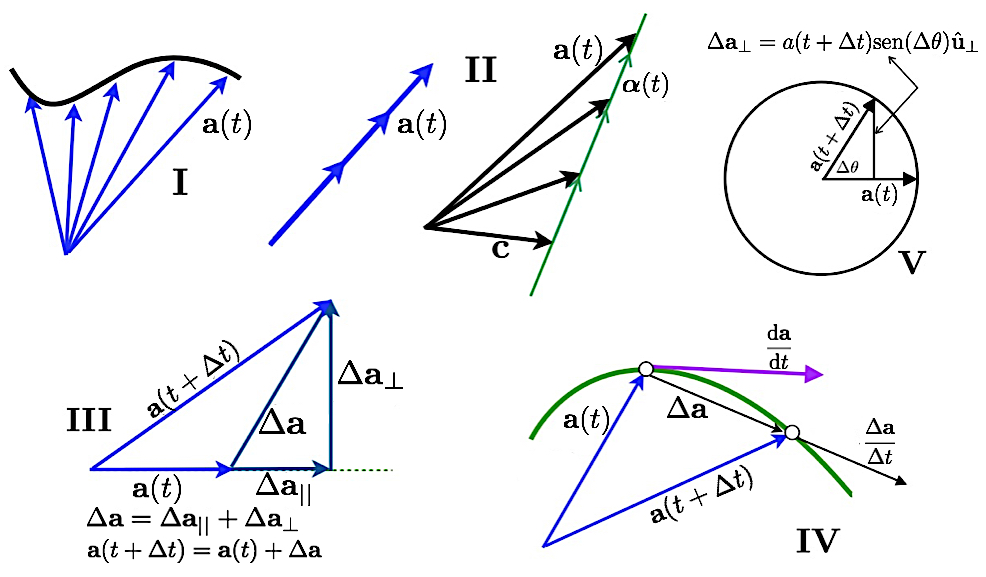
\includegraphics[height=3.4in,width=5.8in]
{VOLUMEN_1/01_Vectores_Cartesianos/Figuras/Figura1_9.jpg}
\caption{Vectores variables}
\label{fig6vectcartes}
\end{center}
\end{figure}

Ahora bien, esto implica que:
\begin{equation}
\mathbf{a}(t)  =a^{k}(t)  \mathbf{e}_{k}\left(t\right)  \,\,   \Rightarrow \,\,  
\frac{\mathrm{d}  \mathbf{a}(t)  }{\mathrm{d}t}=
\frac{\mathrm{d}\left[  a^{k}(t) \mathbf{e}_{k}(t)  \right]  }{\mathrm{d}t}=
\frac{\mathrm{d} a^{k}(t)   } {\mathrm{d}t}\mathbf{e}_{k}\left(t\right)  + a^{k}(t)  \frac{\mathrm{d }  \mathbf{e}_{k}(t)  }{\mathrm{d}t} \,,
\label{dAdtvariable}
\end{equation}
con lo cual hay que tener cuidado al derivar vectores y cerciorarse de la dependencia funcional de la base y componentes. 

Habr� sistemas de coordenadas (bases de vectores) que ser�n constantes y otros en los cuales sus vectores bases cambiar�n en su direcci�n. El primer t�rmino de (\ref{dAdtvariable}) representa la variaci�n del m�dulo, y el segundo
muestra la contribuci�n de los cambios en direcci�n del vector. M�s a�n, mostraremos apoy�ndonos en la ilustraci�n de el cuadrante III de la figura \ref{fig6vectcartes} que, independientemente del sistema
de coordenadas, el cambio en el m�dulo apunta en la direcci�n del vector, mientras que las contribuciones en direcci�n apuntan en la direcci�n perpendicular al vector. Esto es:
\[
\frac{\mathrm{d}\mathbf{a}\left(t\right)}{\mathrm{d}t}=
\frac{\mathrm{d} \left|  \mathbf{a}(t)  \right| }{\mathrm{d}t}\hat{{\bf u}}_{\Vert} +\left|  \mathbf{a}\left(t\right)  \right| \hat{{\bf u}}_{\bot}\,, \quad \text{con }\hat{{\bf u}}_{\Vert} \cdot \hat{{\bf u}}_{\bot}=0\,.
\label{dAdt2}
\]

Es f�cil convencernos de la forma del primer t�rmino. Siempre podemos representar un vector como su m�dulo y un vector unitario en la direcci�n apropiada. Esto es:
\[
\mathbf{a} (t)  =\left|  \mathbf{a}(t)  \right| \hat{\bf u}(t) \,\,  \Rightarrow \,\,   \frac{\mathrm{d} \mathbf{a} (t)}{\mathrm{d}t}=
\frac{\mathrm{d}\left[  \left|  \mathbf{a}\left(t\right)  \right|  \hat{\bf u}(t)  \right]  }{\mathrm{d}t}=
\frac{\mathrm{d }\left|  \mathbf{a}(t)  \right|  }{\mathrm{d}t}\hat{\bf u}(t)  +\left|  \mathbf{a}(t)\right|\frac{\mathrm{d}  \hat{\bf u}(t)}{\mathrm{d}t} \,.
\]
Por ser $|\hat{\bf u}(t)|=1$, resulta que $\hat{\bf u}(t)\cdot \frac{\mathrm{d}  \hat{\bf u}(t)}{\mathrm{d}t}=0$, es decir, son perpendiculares. 

Como podemos ver a continuaci�n cuando multiplicamos por $\hat{\bf u}(t)$:

\[
\hat{\bf u}(t) \cdot \frac{\mathrm{d} \mathbf{a}\left(t\right)}{\mathrm{d}t}=
\hat{\bf u}(t)  \cdot\left[\frac{\mathrm{d}\left|  \mathbf{a}(t)  \right|  }{\mathrm{d}t} \hat{\bf u}(t)  +\left|  \mathbf{a}(t)  \right|\frac{\mathrm{d} \hat{\bf u}(t)   }{\mathrm{d}
t}\right] \,\,  \Rightarrow \,\,  
\left\{
\begin{array}
[c]{c}
\hat{\bf u}(t)  \cdot \dfrac{\mathrm{d} \mathbf{a}\left(t\right)   }{\mathrm{d}t}=\dfrac{\mathrm{d }\left| \mathbf{a}\left(t\right)  \right|  }{\mathrm{d}t}\\
\\
\hat{\bf u}(t)  \cdot\dfrac{\mathrm{d} \hat{\bf u}\left(t\right)  }{\mathrm{d}t}=0
\end{array}
\right.
\]

Es decir que el cambio en el m�dulo de un vector se manifiesta en la direcci�n del mismo vector, tal y como era intuitivo suponer. Adicionalmente,  vemos que el vector $\hat{\bf u}$ siempre ser� perpendicular a su derivada. Gr�ficamente
podemos apreciarlo en el cuadrante IV de la figura \ref{fig6vectcartes}, pero tambi�n surge anal�ticamente si derivamos el vector unitario en la direcci�n de $\mathbf{a}(t)$:
\[
\frac{\mathrm{d}\left[  \hat{\bf u}(t)  \cdot \hat{\bf u}\left(t\right)  \right]  }{\mathrm{d}t}\equiv
\frac{\mathrm{d}\left(  \left|  \hat{\bf u}(t)  \right|  ^{2}\right)  }{\mathrm{d}t}=
\frac{\mathrm{d}\left(  1\right)  }{\mathrm{d}t}\equiv 0 =
\hat{\bf u}\left(t\right)  \cdot \frac{\mathrm{d}  \hat{\bf u}(t) }{\mathrm{d}t}
\,\,  \Rightarrow \,\,   
\hat{\bf u}(t)  \ \bot \ \frac{\mathrm{d} \hat{\bf u}(t)   }{\mathrm{d}t} \,,
\]
es decir:
\[
\frac{\mathrm{d}  \mathbf{a}(t)  }{\mathrm{d}t}=
\frac{\mathrm{d}\left[  \left|  \mathbf{a}(t)  \right|  \hat{\bf u} (t)  \right]  }{\mathrm{d}t}=
\frac{\mathrm{d}\left| \mathbf{a}(t)  \right|  }{\mathrm{d}t}\hat{\bf u}(t) +\left|  \mathbf{a}(t)  \right|  \frac{\mathrm{d}  \hat{\bf u} (t)  }{\mathrm{d}t}=\frac{\mathrm{d}  \left| \mathbf{a}(t)  \right|   }{\mathrm{d}t} \hat{\bf u}_{\Vert}+\left|  \mathbf{a}(t)  \right|  \hat{\bf u}_{\bot}\,.
\]

Supongamos que ahora definimos un vector 
$ \Delta {\boldsymbol \theta} =\Delta \theta \ \hat{\bf v}$, 
con:
\[
\left.
\begin{array}
[c]{c}
\hat{\bf v}\ \bot\ \hat{\bf u}_{\Vert}\\
\\
\hat{\bf v}\ \bot\ \hat{\bf u}_{\bot}
\end{array}
\right\}  \,\,  \Rightarrow \,\,    \left\{
\begin{array}
[c]{c}
\hat{\bf v}\times\hat{\bf u}_{\Vert}=\hat{\bf u}_{\bot}\\
\\
\hat{\bf u}_{\bot}\times\hat{\bf v}=\hat{\bf u}_{\Vert}\\
\\
\hat{\bf u}_{\Vert}\times\hat{\bf u}_{\bot}=\hat{\bf v}
\end{array}
\right.
\]
donde $\Delta {\boldsymbol \theta} $ es el �ngulo de rotaci�n del vector ${\bf a}(t) $ (ver cuadrante V de la figura \ref{fig6vectcartes}). Claramente:
\begin{align*}
\Delta\mathbf{a}_{\bot}  &  =\left[a\left( t+\Delta t\right)  
\operatorname{sen}\left(  \Delta
\theta\right)\right]  \hat{\bf u}_{\bot}\approx \left[a\left(t+\Delta t\right)
\Delta\theta\right] \hat{\bf u}_{\bot} \,\,  \Rightarrow \,\,    \Delta \mathbf{a}_{\bot} = \Delta {\boldsymbol \theta} \times\mathbf{a}(t) \,,
\end{align*}
entonces:
\begin{equation*}
\dfrac{\Delta\mathbf{a}_{\bot}}{\Delta t}   \equiv\left[  \frac{\Delta\mathbf{a}
}{\Delta t}\cdot \mathbf{a}_{\bot}\right]  \mathbf{a}_{\bot}=
\frac{ \Delta {\boldsymbol \theta} }{\Delta t}\times\mathbf{a}\left(t\right) 
\,\,  \Rightarrow \,\,   
\left[  \frac{\mathrm{d}\mathbf{a}\left(t\right) }
{\mathrm{d}t}\cdot\hat{\bf u}_{\bot}\right]  \hat{\bf u}_{\bot}=\frac{\mathrm{d}
  \theta(t)  }{\mathrm{d}t}\hat{\bf v}\times
\mathbf{a}(t)  =  {\boldsymbol \omega} \times\mathbf{a}(t) \,,
\end{equation*}
donde hemos identificado ${\boldsymbol \omega}=\frac{\mathrm{d} \theta\left( t\right)}{\mathrm{d}t}\hat{\bf v}$. 

Podemos ir m�s all� observando el cuadrante V de la figura \ref{fig6vectcartes}, vemos que si suponemos que el m�dulo del vector es constante, entonces:
\[
\dfrac{\mathrm{d }\left| \mathbf{a}(t)  \right|  }{\mathrm{d}
t}=0 \quad  \Rightarrow \quad  \frac{\mathrm{d}  \mathbf{a}(t) }{\mathrm{d}t}=
\left|  \mathbf{a}(t)  \right|  \hat
{\bf u}_{\bot} \,\,  \Rightarrow \,\,    \left[  \frac{\mathrm{d}  \mathbf{a}\left(
t\right) }{\mathrm{d}t}\cdot\hat{\bf u}_{\bot}\right]  \hat{\bf u}_{\bot
}={\boldsymbol \omega} \times\mathbf{a}(t)\,.
\]

\subsection{Velocidades y aceleraciones}
\label{VelocidadesAceleraciones3D}
\index{Vectores 3D!Velocidades/Aceleraciones}
El radio vector posici�n de una part�cula genera, como sabemos,  los vectores velocidad y aceleraci�n:
\[
{\bf r}={\bf r}(t)  \,\,  \Rightarrow \,\, {\bf v}(t)=
\frac{\mathrm{d}  {\bf r} (t)  }{\mathrm{d}t} \,\,  \Rightarrow \,\, {\bf a}(t)  =\frac{\mathrm{d} {\bf v} (t)  }{\mathrm{d}t}=\frac{\mathrm{d}^{2}{\bf r}(t)  }{\mathrm{d}t^{2}}\,,
\]
ahora bien:
\[
{\bf r}=r\hat{\bf u}_{r}=x{{\bf i}}+y{{\bf j}}+z{{\bf k}}\,, \quad\text{con: } \ \hat{\bf u}
_{r}=\cos(\theta)\ {{\bf i}}+\operatorname{sen}(\theta)\ {{\bf j}} + z{{\bf k}}\,.
\]

Si suponemos que la part�cula describe una trayectoria, entonces:
\[
\left.
\begin{array}
[c]{c}
r=r(t) \\
\\
\theta=\theta(t)\\
\\
z=z(t)
\end{array}
\right\}  \quad\Longleftrightarrow\quad\left\{
\begin{array}
[c]{c}
x=x(t) \\
y=y(t) \\
z=z(t)
\end{array}
\right.  ;\quad\hat{\bf u}_{r}=\hat{\bf u}_{r}\left(t\right)  ;\quad
\begin{array}
[c]{c}
{{\bf i}}=\text{const}\\
{{\bf j}}=\text{const}\\
{{\bf k}}=\text{const}
\end{array}
\]

Es muy com�n denotar a la derivada temporal sobre funciones de una variable con un punto, es decir, podemos utilizar la siguiente notaci�n:
\[
 \dot{f}(t) \equiv \frac{\mathrm{d} f \left(t\right)}{\mathrm{d}t} \,,
\]
con lo cual, y en el caso de que  $z=z(t)=$ constante, se tiene:
\begin{eqnarray*}
\frac{\mathrm{d}  \hat{\bf u}_{r} }{\mathrm{d}t}  & =&
\frac{\mathrm{d}\left[  \cos(\theta\left(t\right))  {{\bf i}}
+\operatorname{sen}(\theta\left(t\right) ) {{\bf j}}\right]  }{\mathrm{d}t}=
\dot{\theta}(t) \underset{\hat{\bf u}_{\theta}
}{\underbrace{\left[  - \operatorname{sen}(\theta(t) )
{{\bf i}}+\cos(\theta(t) ) {{\bf j}
}\right]  }}=\dot{\theta}(t) \hat{\bf u}_{\theta}\,.
\end{eqnarray*}

Ya que:
\begin{align*}
\left|  \hat{\bf u}_{r}\right|   &  =\sqrt{\hat{\bf u}_{r}\cdot\hat{\bf u}_{r}}
=\sqrt{\left[  \cos(\theta(t))  \ {{\bf i}}+\operatorname{sen}
(\theta(t))  \ {{\bf j}}\right] \cdot \left[  \cos(
\theta(t))  \ {{\bf i}}+\operatorname{sen}(\theta(t))
\ {{\bf j}}\right]  }=1 \,,\\
& \\
\left|  \hat{\bf u}_{\theta}\right|   &  =\sqrt{\hat{\bf u}_{\theta}\cdot\hat
{\bf u}_{\theta}}=\sqrt{\left[  -  \operatorname{sen}(\theta(t))
\ {{\bf i}}+\cos(\theta(t) ) \ {{\bf j}
}\right]  \cdot \left[  -\left(  \operatorname{sen}(\theta(t)  \right))  {
{\bf i}}+\cos(\theta(t))  {{\bf j}}\right]  }=1 \,.
\end{align*}
Entonces:
\[
\hat{\bf u}_{\theta}\cdot\hat{\bf u}_{r}=\hat{\bf u}_{r}\cdot\hat{\bf u}_{\theta}=\left[
-  \operatorname{sen}(\theta(t))  \ {{\bf i}}
+\cos(\theta(t))  \ {{\bf j}}\right] \cdot \left[
\cos(\theta(t)) \ {{\bf i}}+\operatorname{sen}(\theta\left(
t\right))  \ {{\bf j}}\right]  =0 \,.
\]

Adem�s:
\[
\frac{\mathrm{d}  \hat{\bf u}_{\theta} }{\mathrm{d}t}=\frac
{\mathrm{d} \left[ -\mbox{sen}(\theta(t)) 
\ {{\bf i}}+\cos(\theta(t))  \ {{\bf j}}\right]  }{\mathrm{d}t}= -\dot{\theta}(t) \left[\cos(\theta(t)) \ {{\bf i}}+\operatorname{sen}(\theta(t))  \ {{\bf j}}\right]
=-\dot{\theta}(t) \hat{\bf u}_{r} \,.
\]

Para una part�cula que sigue un movimiento arbitrario, su trayectoria vendr� descrita, en coordenadas cartesianas, por:
\[
{\bf r}=x (t)  \ {{\bf i}}+y(t)\ {{\bf j}}+z(t) \ {{\bf k}}\,.
\]
\begin{itemize}
\item Su velocidad ser�:
\begin{align*}
{\bf v}(t)   &  =\frac{\mathrm{d}{\bf r}(t)}{\mathrm{d}t}=\frac{\mathrm{d}\left[ x(t)  {
{\bf i}}+y(t)  {{\bf j}}+z(t){{\bf k}}\right] }{\mathrm{d}t}=
\dot{x}(t) {{\bf i}}+\dot{y}(t){{\bf j}}+\dot{z}(t) {{\bf k}}
=v_{x}(t)  {{\bf i}}+v_{y}(t){{\bf j}}+v_{z}(t)  {{\bf k}} \,.
\end{align*}
\item Y su aceleraci�n:
\[
{\bf a}(t)  =
\dot{v}_x(t) {{\bf i}}+\dot{v}_y(t)   {{\bf j}}+\dot{v}_z(t) {{\bf k}}=
a_{x}(t)  {{\bf i}}+a_{y}\left(t\right)  {{\bf j}}+a_{z}(t)  {{\bf k}}\,.
\]
\end{itemize}

Mientras que en coordenadas polares las ecuaciones son:
\[
{\bf r}(t)  =r(t)  \hat{\bf u}_{r}(t) \,.
\]
\begin{itemize}
\item Velocidad: 
\[
{\bf v}(t)  =\frac{\mathrm{d}\left[  r\left(t\right)\hat{\bf u}_{r}(t)  \right]  }{\mathrm{d}t}=
\dot{r}(t) \hat{\bf u}_{r}(t)  +r(t)\frac{\mathrm{d}\hat{\bf u}_{r}(t)  }{\mathrm{d}t}=
\dot{r}(t) \hat{\bf u}_{r}\left( t\right)  +r(t) \dot{\theta}(t)\hat{\bf u}_{\theta}(t) \,,
\]
\item Aceleraci�n:
\begin{align*}
{\bf a}(t)   &  =\frac{\mathrm{d}{\bf v}(t) }{\mathrm{d}t}=
\frac{\mathrm{d}\left[  \dot{r}(t) \hat{\bf u}_{r}(t)  + 
r(t) \dot{\theta}(t)  \hat{\bf u}_{\theta}(t)  \right]  }{\mathrm{d}t}=
\frac{\mathrm{d}\left[\dot{r} \left(t\right)\hat{\bf u}_{r}(t)  \right]  }{\mathrm{d}t}+
\frac{\mathrm{d}\left[ r(t)\dot{\theta}(t)\hat{\bf u}_{\theta}\left(t\right)  \right]  }{\mathrm{d}t}\\
& \\
&  = \ddot{r}(t)
\hat{\bf u}_{r}\left(t\right)  +
\dot{r}(t) \frac{\mathrm{d}  \hat{\bf u}_{r}(t)   }{\mathrm{d}t}+
\dot{r}(t)\dot{\theta}(t)\hat{\bf u}_{\theta}\left(t\right)  +
r(t) \ddot{\theta}(t) \hat{\bf u}_{\theta}(t)  +
r(t) \dot{\theta}(t) \frac{\mathrm{d}  \hat{\bf u}_{\theta}(t)  }{\mathrm{d}t}\\
& \\
&  =
\left\{ \ddot{r}(t) -r (t)\left( \dot{\theta}(t) \right)^{2}\right\}  \hat{\bf u}_{r}(t)  +
\left\{2\ \dot{r}(t) \dot{\theta}(t) +r(t) \ddot{\theta}(t) \right\}  \hat{\bf u}_{\theta}(t) \,.
\end{align*}
\end{itemize}

Claramente para el caso de un movimiento circular, donde $r=R=\text{const}$, resulta:
\[
\frac{\mathrm{d}R}{\mathrm{d}t}=0\quad  \Rightarrow \quad  \left\{
\begin{array}
[c]{l}
{\bf r}(t)  =R\ \hat{\bf u}_{r}(t)\\
\\
{\bf v}(t)  =R\ \dot{\theta}(t) \hat{\bf u}_{\theta}\\
\\
{\bf a}(t)  =-R\  \dot{\theta}(t)^{2}\hat{\bf u}_{r}(t)  +R\ \ddot{\theta}(t)\hat{\bf u}_{\theta}(t)
\end{array}
\right.
\]

De aqu� podemos ver que el vector velocidad ${\bf v}(t)$ y el vector  posici�n ${\bf r}(t) $ son ortogonales. La velocidad, ${\bf v}(t),$ siempre es tangente a la trayectoria $\bf {r}\left(t\right)$ y en este caso la trayectoria es una circunferencia. 

En general el vector:
\[
{\bf r}_{med}= \sum_{i} \Delta{\bf r}(t_{i})  = \sum_{i} \left({\bf r}\left(  t_{i}+\Delta t_{i}\right)  -{\bf r}(t_{i}) \right)  
\,\,  \Rightarrow \,\,  \lim_{\Delta t\rightarrow0} \sum_{i}\Delta{\bf r}(t_{i}) = 
\int\mathrm{d}{\bf r}(t)={\bf r}(t) \,,
\]
es decir, $\mathrm{d}{\bf r}(t)  =\lim_{\Delta t\rightarrow0} \sum_{i}\Delta\ {\bf r}(t_{i})$ es tangente a la trayectoria.
Es claro que:
\[
\mathrm{d}{\bf r}(t)  =\mathrm{d}\left[  x(t) {{\bf i}}+y(t)  {{\bf j}}+z(t)  {{\bf k}}\right]  \equiv
\frac{\mathrm{d} x(t)  }{\mathrm{d} t}{{\bf i}}+ \frac{\mathrm{d} y(t)  }{\mathrm{d} t}{{\bf j}}+ \frac{\mathrm{d} z(t)  }{\mathrm{d} t}{{\bf k}} \,.
\]

Tal y como mencionamos arriba, para el sistema de coordenadas cartesiano podemos definir un vector (en este caso) velocidad angular ${\boldsymbol \omega}$ tal que:
\[
\left.
\begin{array}
[c]{c}
\dfrac{ {\boldsymbol \omega} }{\left| {\boldsymbol \omega}  \right|  }\times\hat{\bf u}_{r}=
\hat{\bf u}_{v}\\
\\
\hat{\bf u}_{v} \times \dfrac{{\boldsymbol \omega}  }{\left| {\boldsymbol \omega} \right|}=
\hat{\bf u}_{r}\\
\\
\hat{\bf u}_{r} \times \hat{\bf u}_{v}=
\dfrac{{\boldsymbol \omega}  }{\left|{\boldsymbol \omega} \right|  }
\end{array}
\right\}  \quad  \Rightarrow \quad  {\bf v}(t)  ={\boldsymbol \omega}  \times {\bf r}(t) \,.
\]

Supongamos por simplicidad que elegimos el sistema de coordenadas cartesiano, donde  ${\bf r}$ est� en el plano $xy$.  En este caso es inmediato comprobar que $v^{i}=\varepsilon^{ijk}\omega_{j}x_{k}$, y dado que ${\bf r}$ y ${\bf v}$ tienen �nicamente componentes $1$ y $2$ entonces, necesariamente  ${\boldsymbol \omega} $ tiene �nicamente  componente $3$,  Es decir:
\[
\left.
\begin{array}
[c]{c}
{\bf r}=r^{i} {\bf e}_{i}\\
\\
{\bf v}=v^{i} {\bf e}_{i}
\end{array}
\right\}  \,\,  \Rightarrow \,\, \left\{
\begin{array}
[c]{c}
v^{1}=\varepsilon^{1j2}\omega_{j}x_{2}\\
\\
v^{2}=\varepsilon^{2j1}\omega_{j}x_{1}
\end{array}
\right\}  \,\,  \Rightarrow \,\,  {\boldsymbol \omega}=
\left| {\boldsymbol \omega} \right|   \mathbf{\textsf{e}}_{3}=
\omega {{\bf k}} \,,
\]
como ${\bf r}=x(t) {{\bf i}}+y(t) {{\bf j}}$, entonces:
\[
{\bf v}(t)  =\frac{\mathrm{d}  {\bf r}(t)  }{\mathrm{d}t}=v_{x}(t)   {{\bf i}}
+v_{y}(t)  {{\bf j}}={\boldsymbol \omega}  \times
{\bf r}(t)  =\dot{\theta}(t) {{\bf k}}\times\left[ x(t)
 {{\bf i}}+y(t)  {{\bf j}}\right] \,.
\]

Se ver� m�s claro en coordenadas polares, esto es:
\begin{align*}
{\bf v}(t)  =\frac{\mathrm{d} {\bf r}(t) }{\mathrm{d}t}
=& r(t) \dot{\theta}(t) \hat{\bf u}_{\theta}(t)  =
\left[  \left|{\boldsymbol \omega} \right|  \hat{\bf u}_{n}(t)  \right]  \times\left[
r(t) \hat{\bf u}_{r}(t)  \right] \,, \quad \quad  \left|  {\bf r}(t)  \right|  =\mbox{const} \\
= & \underset{{\bf v}_{\bot}}{\underbrace{r(t) \dot{\theta}(t)} } \hat{\bf u}_{\theta}(t)   
=\left| {\boldsymbol \omega}  \right|  r(t)\hat{\bf u}_{\theta}(t) \,\,  \Rightarrow \,\,  \dot{\theta}(t) \equiv\left|  {\boldsymbol \omega}  \right| \,.
\end{align*}

\subsection{Vectores y funciones}
\label{VectoresFunciones}
Antes de continuar con la integraci�n repensemos algunas funciones de tipo $\phi\left( x^i\right)$ y ${\bf A} (x^i)$. Estas funciones son sin duda funciones de varias variables, en el caso cartesiano:
\[
\phi =\phi(x,y,z) \,, \quad 
{\bf A} ={\bf A} (x,y,z) = {{\bf i}}A_{x}\left(x,y,z\right)  +{{\bf j}}A_{y}(x,y,z)  +{{\bf k}}A_{z}(x,y,z)\,.
\]

Un par de reflexiones se pueden hacer en este punto, primeramente, dado que hemos relacionado un punto del espacio con el radio vector posici�n, entonces:
\[
P_{(x,y,z)  }\leftrightarrow(x,y,z)  \leftrightarrow
{\bf r}=x\ {{\bf i}}+y\ {{\bf j}}
+z\ {{\bf k}}\,\,  \Rightarrow \,\, \left\{
\begin{array}
[c]{c}
\phi=\phi(x,y,z)  \equiv\phi\left(  {\bf r}\right) \\
\\
{\bf A} ={\bf A} (x,y,z)  \equiv{\bf A} \left(  {\bf r}\right)
\end{array}
\right.
\]

La primera funci�n, $\phi\left({\bf r}\right)$, ser� una funci�n escalar de argumento vectorial o, simplemente un campo escalar y la segunda, ${\bf A} \left({\bf r}\right)$, se conoce como una funci�n vectorial de argumento vectorial o campo vectorial. Como hemos dicho, este tipo de funciones y las operaciones que pueden ser realizadas con ellas, y su significado, ser�n analizadas en detalle m�s adelante durante el desarrollo de este  curso.

En segundo lugar, siempre podremos parametrizar las coordenadas y tendremos
\begin{align*}
\phi &  =\phi(t)  =\phi\left(  x(t)  ,y\left(t\right)  ,z(t)  \right) \,,\\
{\bf A} &  ={\bf A} (t)  ={\bf A} \left( x(t), y(t), z(t)  \right) =
A_{x}\left(  x(t), y\left(t\right)  , z(t)  \right){{\bf i}}  +
A_{y}\left(x(t)  ,y(t)  ,z(t)  \right){{\bf j}} +
A_{z}\left(  x(t)  ,y(t)  ,z\left(t\right)  \right){{\bf k}} \,.
\end{align*}

Este caso lo hemos encontrado en montones de situaciones, por ejemplo, el  movimiento parab�lico viene descrito por  vectores velocidad y posici�n dados por:
\begin{align*}
{\bf v}(t) &  =- gt\ {{\bf k}} +{\bf v}_{0}=-gt\ {{\bf k}}  +
\left(  v_{0x}{{\bf i}} + v_{0y}{{\bf j}}+v_{0z} {{\bf k}} \right)  
\,\,  \Rightarrow \,\,  \left\{
\begin{array}
[c]{l}
v_{x}=v_{0x}\\
v_{y}=v_{0y}\\
v_{z}=v_{0z}-gt
\end{array}
\right. \\
& \\
{\bf r}(t)  &  =-\frac{g}{2}t^{2}\  {{\bf k}}  +{\bf v}_{0}t=
- \frac{g}{2}t^{2} \  {{\bf k}} +\left(  v_{0x}{{\bf i}} + v_{0y}{{\bf j}}+v_{0z} {{\bf k}} \right) t
\,\,  \Rightarrow \,\,  \left\{
\begin{array}
[c]{l}
x=v_{0x}t\\
y=v_{0y}t\\
z=v_{0z}t-\frac{g}{2}t^{2}
\end{array}
\right.
\end{align*}

\subsubsection{Derivada de funciones del tipo: $\phi\left(  {\bf r}(t)
\right)$}

Al derivar una funci�n de argumento vectorial tambi�n se aplica la ``regla de la cadena''. Esto es, si
\[
\phi\left( {\bf r}(t)  \right)  = \phi \left(  x\left(t\right), y(t), z(t)  \right) \,,
\]
entonces:
\begin{align*}
\frac{\mathrm{d}\phi\left( {\bf r}(t)  \right)  }{\mathrm{d}t}  &  =
\frac{\partial \phi\left( x(t) ,y(t)  ,z(t)  \right)  }{\partial x} \frac{\mathrm{d }x(t)  }{\mathrm{d}t}+
\frac{\partial \phi\left( x(t), y(t), z(t)\right) }{\partial y}\frac{\mathrm{d}y(t)  }{\mathrm{d}t}+
\frac{\partial \phi\left(  x(t), y(t), z(t)  \right)  }{\partial z}\frac{\mathrm{d}z(t)}{\mathrm{d }t} \\
& \\
&  =\left[  \frac{\partial \phi\left(
x,y,z\right)  }{\partial x}{{\bf i}}+\frac{\partial
\phi(x,y,z)  }{\partial y}{{\bf j}+}\frac
{\partial \phi(x,y,z)  }{\partial z}{{\bf k}
}\right] \cdot \left[ 
\frac{\mathrm{d }x(t)  }{\mathrm{d }t}{{\bf i}}+
\frac{\mathrm{d }y(t)  }{\mathrm{d }t}{{\bf j}+
\frac{\mathrm{d }z(t)  }{\mathrm{d }t}{\bf k}}\right]\\
& \\
&  ={\boldsymbol \nabla}  \phi\left(  x(t)  ,y\left(t\right)  ,z(t)  \right)  
\cdot\frac{\mathrm{d }{\bf r}\left(t\right)  }{\mathrm{d }t} \,,
\end{align*}
donde hemos representado:
\[
{\boldsymbol \nabla}  \phi\left(  {\bf r}(t)  \right)  \equiv
\frac{\partial \phi(x,y,z)  }{\partial x}{{\bf i}}+
\frac{\partial \phi(x,y,z)  }{\partial y}{\bf j}+
\frac{\partial \phi(x,y,z)} {\partial z}{{\bf k}}=
\partial^{i}\phi\left(  x^j\right) {{\bf i}}_{i}=
\phi^{,i}\left(  x^j\right)  {{\bf i}}_{i} \,,
\]
y lo llamaremos el {\bf gradiente} de la funci�n $\phi\left(  {\bf r}(t)  \right)$.

El gradiente de un campo escalar es uno de los objetos m�s �tiles que encontraremos en el estudio de problemas de F�sica-Matem�tica, el cual lo utilizaremos por ahora de manera operacional. Es bueno recordar que emerge como consecuencia de una derivaci�n contra un par�metro. El gradiente mide el cambio de la funci�n $\phi\left( x,y,z\right) $.

La idea de gradiente nos lleva a considerar a ${\boldsymbol \nabla}$ como un operador vectorial que act�a sobre la funci�n escalar de variable vectorial $\phi\left(  {\bf r}(t)  \right)$.  
\[
{\boldsymbol \nabla}\phi\left(  {\bf r}(t)  \right)   
\equiv\left(\frac{\partial}{\partial x}{{\bf i}}+\frac{\partial}{\partial y}{{\bf j}+}\frac{\partial}{\partial z}{{\bf k}}\right)
\phi(x,y,z) = \mathbf{i}_{i} \ \partial^{i} \phi(x,y,z)\,.
\]
Es decir, y  con un poquito de imaginaci�n:
\[
{\boldsymbol \nabla} \left(  \circ\right)  =\left(  
\frac{\partial }{\partial x}{{\bf i}}+
\frac{\partial }{\partial y}{{\bf j}}+
\frac{\partial }{\partial z}{{\bf k}}\right)
\left(\circ\right)  =\mathbf{{i}}_{i}\partial^{i}\left(  \circ\right)\,.
\]

\subsubsection{Derivada de funciones del tipo: ${\bf A} \left({\bf r}(t)\right) $}
De modo que inspirados en la regla de la cadena de una funci�n escalar de variable vectorial podemos comprobar que:
\[
\frac{\mathrm{d} {\bf A} }{\mathrm{d}t}=
\frac{\mathrm{d} A_{x}\left(x,y,z\right) }{\mathrm{d}t}{{\bf i}}+
\frac{\mathrm{d} A_{y}\left(x,y,z\right) }{\mathrm{d}t}{\bf j}+
\frac{\mathrm{d} A_{z}\left(x,y,z\right) }{\mathrm{d}t}{\bf k}=
\frac{\mathrm{d} A^{i}\left(x^j\right)  }{\mathrm{d}t}{{\bf i}}_{i} \,,
\]
por consiguiente, si ${\bf A} $, tiene por componentes cartesianas $\left( A_{x}, A_{y}, A_{z}\right)$ las componentes del vector derivado ser�n:
$\left(  \frac{\mathrm{d} A_{x}}{\mathrm{d}t},\frac{\mathrm{d} A_{y}
}{\mathrm{d}t},\frac{\mathrm{d} A_{z}}{\mathrm{d}t}\right)$.  Con lo cual, para cada componente:
\[
\frac{\mathrm{d}\left(A^{i}\left(  x(t), y(t), z(t)  \right) \right) }{\mathrm{d}t}=
\frac{\mathrm{d} \left(A^{i}\left(x^{j}(t)  \right) \right) }{\mathrm{d}t}=
\frac{\partial \left(A^{i}\left(x^{j}\right) \right) }{\partial x^{k}}\frac{\mathrm{d} x^{k}(t)}{\mathrm{d}t}=
\left(  \frac{\mathrm{d }{\bf r}(t)}{\mathrm{d }t}\cdot {\boldsymbol \nabla}  \right)  A^{i}(x,y,z)\,.
\]
En t�rminos vectoriales es:
\[
\frac{\mathrm{d} {\bf A} }{\mathrm{d}t}=\left(  \frac{\mathrm{d}{\bf r}(t)  }{\mathrm{d}t}\cdot {\boldsymbol \nabla}  \right)  {\bf A}  \equiv 
\left(  {\bf v}\cdot {\boldsymbol \nabla}  \right)  {\bf A} \,\,  \Rightarrow \,\,
\frac{\mathrm{d} \left(  \circ\right)  }{\mathrm{d}t}=\left(  {\bf v} \cdot {\boldsymbol \nabla}  \right)  \left(  \circ\right)  \equiv v^{i}\partial_{i}\left(  \circ\right)\,,
\]
con ${\bf v}$ la derivada del radio vector posici�n ${\bf r}\left( t\right)$, es decir, la velocidad. Entonces, 
estamos viendo que el cambio del vector ${\bf A} $ respecto al tiempo es el cambio de sus componentes en la direcci�n de la velocidad.

Si se nos ocurre calcular la derivada del vector velocidad para encontrar la aceleraci�n tendremos que nos quedar� expresada como:
\[
{\bf a}=\frac{\mathrm{d} {\bf v}}{\mathrm{d}t}=\left(  {\bf v}\cdot
{\boldsymbol \nabla} \right)  {\bf v}\,\,  \Rightarrow \,\, a^{i}=\left(  {\bf v}\cdot
{\boldsymbol \nabla}\right)  v^{i} \,,
\]
donde las componentes cartesianas de los vectores velocidad y aceleraci�n son: 
$v^{i}=v^{i}\left(  x\left(t\right)  ,y(t)  ,z\left( t\right)  \right)  $ y $\ a^{i}=a^{i}\left(  x(t)  ,y\left(t\right)  ,z(t)  \right)$, respectivamente.

\subsection{El operador ${\boldsymbol \nabla}$}
\label{VectorGradiente}

El operador vectorial ${\boldsymbol \nabla}\left(\circ\right)$ merece un poco de atenci�n en este nivel. Tal y como hemos visto cuando construimos: 

{\bf El Gradiente}:
\begin{eqnarray}
{\boldsymbol \nabla}\phi(x,y,z)   &=&
 \frac{\partial\phi(x,y,z)  }{\partial x} {\bf i} +
\frac{\partial\phi(x,y,z)  }{\partial y}{\bf j}+
\frac{\partial\phi(x,y,z)  }{\partial z} {\bf k} \nonumber \\
& = & 
\partial^{1}\phi(x,y,z) {\bf i}_{1} + 
\partial^{2}\phi(x,y,z) {\bf i}_{2}  + 
\partial^{3}\phi(x,y,z) {\bf i}_{3} = 
\partial^{i} \phi\left(  x^j\right) {\bf i}_{i}\,.
\end{eqnarray}

Podemos ver ahora que existen otras posibilidades:

{\bf El Rotor}: Se puede construir la siguiente operaci�n: ${\boldsymbol \nabla} \times{\bf A}$, que denominaremos  {\bf rotor} de ${\bf A}$, y  vendr� dado por la siguiente expresi�n:
\begin{eqnarray}
{\boldsymbol \nabla} \times{\bf A}  & = &
\left( \frac{\partial}{\partial x} {\bf i}+ \frac{\partial}{\partial y}{\bf j}+ \frac{\partial}{\partial z} {\bf k} \right)  
\times\left(  A_{x} {\bf i}+A_{y} {\bf j}+A_{z} {\bf k}\right) \nonumber \\
&  = &
\left(  \frac{\partial A_{z}}{\partial y}-\frac{\partial A_{y}}{\partial z}\right)  {\bf i} +
\left(\frac{\partial A_{x}}{\partial z}-\frac{\partial A_{z}}{\partial x}\right){\bf j}+
\left(  \frac{\partial A_{y}}{\partial x}-\frac{\partial A_{x}}{\partial y}\right) {\bf k} = \varepsilon^{ijk}\partial_{j}A_{k}\ {\bf i}_i \,.
\end{eqnarray}

{\bf La Divergencia}: Tambi�n podemos hablar del ``producto escalar'' de nabla por un vector ${\bf A}$. 
A esta operaci�n la llamaremos {\bf divergencia} de ${\bf A}$:
\[
{\boldsymbol \nabla} \cdot{\bf A}=\frac{\partial A^{i}\left(  x^{j}\right)}
{\partial {x}^{i}}\equiv\partial_{i}A^{i}\left(  x^{j}\right)
\equiv\frac{\partial A_{x}(x,y,z)  }{\partial x}+\frac{\partial
A_{y}(x,y,z)}{\partial y}+\frac{\partial A_{z}\left(
x,y,z\right)  }{\partial z} \,,
\]
pero por ahora consideremos nabla ${\boldsymbol \nabla}$ como un vector. 


De este modo habr� una gran cantidad de relaciones vectoriales  que involucran a ${\boldsymbol \nabla}$, las cuales se podr�n demostrar.


\subsection{Integraci�n}
\label{IntegracionCartesianas}
\index{Integraci�n vectores 3D}
\index{Vectores 3D!Integraci�n}

Despu�s de haber diferenciado campos escalares y vectoriales, el siguiente paso es integrarlos. Encontraremos algunos objetos vectoriales a integrar y ser�n:

\begin{itemize}
\item Integraci�n de un vector por un escalar: 
\[
\int{\bf A} \left(  u\right)  \ \mathrm{d} u
\]
\item Integraci�n de un escalar a lo largo de un vector:
\[
\int_{c}\phi(x,y,z)  \ \mathrm{d}{\bf r}
\]
\item Integraci�n de un vector a lo largo de otro vector:
\[
\int_{c}{\bf A} (x,y,z)  \cdot\mathrm{d} {\bf r}
\]
\end{itemize}

El primero de los casos es el tipo de integral que siempre hemos utilizado para encontrar la posici�n a partir de la velocidad. Los siguientes tres casos se conocen con el nombre de integrales de l�nea por cuanto es importante la ``ruta'' o trayectoria que sigamos al integrar. Esto aparece indicado por la letra $C$ en la integral y ser� evidente m�s adelante. En general la integral de l�nea depender� de la trayectoria.

\subsubsection{Un vector por un escalar: $\int{\bf A} \left(  u\right)  \ \mathrm{d} u$}

El primer caso de este tipo integrales es el trivial que ya sabemos calcular:
\[
\int{\bf A} \left(u\right)  \ \mathrm{d}u= 
{\bf i} \int A_{x}\left(u\right) \mathrm{d} u+
{\bf j} \int A_{y}\left(u\right)   \mathrm{d} u+
{\bf k} \int A_{z}\left(u\right)  \mathrm{d} u=\left(  \int A^{i}\left(  u\right) \mathrm{d} u\right) \mathbf{{i}}_{i} \,.
\]
La integral de un vector (en un sistema de coordenadas cartesianas) por un escalar se convierte en la suma de tres integrales, cada una a lo largo de las componentes cartesianas del vector.

Recordemos que as� integramos la aceleraci�n en un movimiento parab�lico:
\[
\frac{\mathrm{d}{\bf v}}{\mathrm{d}t}={\bf a}=-g \ \mathbf{{k}}
\,\,  \Rightarrow \,\,   {\bf v}=\int{\bf a}\ \mathrm{d}t=\mathbf{{k}}\
\int-g\ \mathrm{d}t=-\mathbf{{k}}\ gt\ +{\bf v}_{0}=-\mathbf{{k}}gt\ +\mathbf{{i}}v_{0x}+\mathbf{{j}}v_{0y}+\mathbf{{k}}v_{0z} \,.
\]

Ahora bien, existen sutilezas en este caso que debemos tener en cuenta. Por ejemplo, considere la integral:
\[
\int\mathrm{d}t\ \left(  {\bf a}\times\frac{\mathrm{d}^{2}{\bf a}
}{\mathrm{d}t^{2}}\right)  =\int\mathrm{d}t \left(  \frac{\mathrm{d}
 }{\mathrm{d}t}\left(  {\bf a}\times\frac{\mathrm{d} {\bf a}}{\mathrm{d}
t}\right)  -\frac{\mathrm{d} {\bf a}}{\mathrm{d}t}\times\frac{\mathrm{d}
 {\bf a}}{\mathrm{d}t}\right)  =\int\mathrm{d}t\ \frac{\mathrm{d}
 }{\mathrm{d}t}\left(  {\bf a}\times\frac{\mathrm{d} {\bf a}}{\mathrm{d}
t}\right)  ={\bf a}\times\frac{\mathrm{d}{\bf a}}{\mathrm{d}t}+{\bf c} \,.
\]

Pero en general los casos quedan resueltos integrando componente a componente con la ayuda de la notaci�n de �ndices:
\[
\int\mathrm{d}t\ \left(  {\bf a}\times{\bf b}\right)  =\left[  \int
\mathrm{d}t\ \left(  \varepsilon^{ijk}a_{j}b_{k}\right)  \right]  \mathbf{i}_{i}\,.
\]

\subsubsection{Un escalar a lo largo de un vector: $\int_{C}\phi\left(  {\bf r}\right)\mathrm{d}{\bf r}$}

El segundo objeto que ``tropezaremos'' es la integraci�n de funciones de varias variables a lo largo de  una curva determinada. Esto es:
\[
\int_{C}\phi\left(x,y,z\right)  \mathrm{d}{\bf r}=
\int_{C}\phi(x^i)  \left(  
\mathrm{d}x {\bf i} +\mathrm{d}y {\bf j}+\mathrm{d}z {\bf k}\right)  =
{\bf i}\int_{C}\phi(x^i)  \mathrm{d}x+{\bf j}
\int_{C}\phi(x^i)  \mathrm{d} y+ 
{\bf k} \int_{C}\phi(x^i)  \mathrm{d} z\,.
\]

La integral se nos ha convertido en tres integrales, las cuales son ahora componentes de un vector. Esto es posible dado que la base $\left( {\bf i}, {\bf j}, {\bf k} \right)  $ es una base constante. Ahora bien, cada una de estas integrales son interdependientes, dado que hay que seguir la misma curva $C$. 


\subsubsection{Un vector a lo largo de otro vector: $\int_{C}{\bf F} \left({\bf r}\right)  \cdot\mathrm{d}{\bf r}$}
 
Quiz� la integral de l�nea m�s conocida sea una del tipo $\int _{C}{\bf F}\left(  {\bf r}\right) \cdot \mathrm{d}{\bf r}$ 
por cuanto nos la hemos ``tropezado'' en el c�lculo del trabajo que realiza una fuerza. Todo lo que hemos considerado al parametrizar la curva en el caso anterior, sigue siendo v�lido.
\[
\int_{C}{\bf F}\left(  {\bf r}\right) \cdot \mathrm{d}{\bf r}=\int_{C}
F_{x}(x,y,z)  \ \mathrm{d}x+\int_{C}F_{y}(x,y,z)
\ \mathrm{d}y+\int_{C}F_{z}(x,y,z)  \ \mathrm{d}z=\int_{C}
F^{i}\left(  x^{j}\right)  \ \mathrm{d}x_{i} \,.
\]


\subsection{{\color{Fuchsia}Ejemplos}}
\label{EjemDerVectores}
\begin{enumerate}
\item Si una part�cula se mueve a lo largo de una curva descrita por: 
\[
x(t) = 3 t^{2} \,, \quad y(t) = 4t^{3} -t\,, \quad z(t) = t \,.
\]
Entonces, las expresiones para los vectores: posici�n, velocidad y aceleraci�n de esa part�cula son:
\[
{\bf r}(t) = 3 t^{2} {\bf i} + (4t^{3} -t ){\bf j} + t{\bf k} \,,\quad 
{\bf{v}} = 6 t {\bf i} + (12t^{2} -1 ){\bf j} + {\bf k} \,, \quad
{\bf a} = 6  {\bf i} + 24t {\bf j} \,.
\]

Si nos proponemos encontrar las expresiones, m�s generales, de los vectores tangentes y perpendiculares a todo punto de la trayectoria de la part�cula podemos ver que el vector  tangente a todo punto de la trayectoria es el vector velocidad
\[
 {\bf v} = 6 t {\bf i} + (12t^{2} -1 ){\bf j} + {\bf k}\,,
\]

El vector perpendicular a todo punto, ser� un vector ${\bf b} =b_{x} {\bf i} + b_{y}{\bf j} + b_{z}{\bf k}$, tal que:
\[
( 6 t {\bf i} + (12t^{2} -1 ){\bf j} + {\bf k})\cdot (b_{x} {\bf i} + b_{y}{\bf j} + b_{z}{\bf k}) =
6 t b_{x} + (12t^{2} -1 )b_{y} + b_{z} =0\,,
\]
con lo cual:
\[
{\bf b} = b_{x} {\bf i} + b_{y}{\bf j} - (6 t b_{x} + (12t^{2} -1 )b_{y}){\bf k}\,.
\]


\item  La trayectoria de un punto en el plano vista por un observador $(1)$ es la siguiente:
\[
{\bf r}_{1} ( t )  =5 \cos(3t^{2})\ {\bf i} +5\operatorname{sen}(3t^{2})\ {\bf j} \,.
\]

Queremos expresar las aceleraciones radiales y tangenciales de esta part�cula ya que es claro que la part�cula describe un movimiento circular, donde $\theta(t) = 3t^{2}$. Entonces:
\[
{\bf r}(t) = 5 \hat{\bf u}_{r} \,\, \Rightarrow \,\, {\bf v}(t) = \frac{\mathrm{d}{\bf r}(t)}{\mathrm{d}t} = 5  \frac{\mathrm{d} \theta(t)}{\mathrm{d}t}  \hat{\bf u}_{\theta} = 30 t \; \hat{\bf u}_{\theta} \,\, \Rightarrow \,\,
{\bf a}(t) = \frac{\mathrm{d}{\bf a}(t)}{\mathrm{d}t} = 30 \; \hat{\bf u}_{\theta}  -30t \; \hat{\bf u}_{r} \,.
\]

Consideremos ahora un segundo observador $(2)$, el cual describe una trayectoria respecto al primero representada por:
\[
{\bf r}_{21}(t)  = (  t^{3}- 4t) {\bf i}+ (  t^{2}+4t )  \ {\bf j}\,.
\]

Y queremos encontrar las expresiones para los vectores posici�n, velocidad y aceleraci�n de la part�cula medidos respecto al segundo observador.

Por lo tanto, la trayectoria de la part�cula respecto al segundo observador ser�:
\[
{\bf r}_{2}(t) = {\bf r}_{1}(t) - {\bf r}_{21}(t) = 5 \cos(3t^{2})\ {\bf i} +5\operatorname{sen}(3t^{2})\ {\bf j} -((  t^{3}- 4t) {\bf i}+ (  t^{2}+4t )  \ {\bf j}) \,,
\]
con lo cual:
\[
{\bf r}_{2}(t) = \left[5\cos(3t^{2}) - t^{3}+ 4t\right] {\bf i} + 
\left[5\operatorname{sen}(3t^{2}) - t^{2}-4t\right] {\bf j} \,,
\]
entonces:
\[
{\bf v}_{2}(t) =\frac{\mathrm{d}{\bf r}_{2}(t)}{\mathrm{d}t} = 
-\left[30\,\mbox{sen} \left( 3\,{t}^{2} \right) t+3\,{t}^{2}-4 \right] {\bf i} + 
\left[30\,\cos\left( 3\,{t}^{2} \right) t-2\,t-4\right] {\bf j} \,,
\]
y
\[
{\bf a}_{2}(t) =\frac{\mathrm{d}{\bf v}_{2}(t)}{\mathrm{d}t} = 
-6\left[30\cos\left( 3{t}^{2} \right){t}^{2}+5\mbox{sen}\left(3{t}^{2} \right) 
+t\right] {\bf i} - 
2\left[90\mbox{sen}\left( 3{t}^{2} \right) {t}^{2}-15\cos\left( 3{t}^{2} \right) +1\right] {\bf j} \,.
\]

\item Demostrar que: 
\[
{\boldsymbol \nabla}\left(  {\bf a}\cdot{\bf b} \right) =\left({\bf a}
\cdot{\boldsymbol \nabla}\right)  {\bf b}+\left(  {\bf b}\cdot{\boldsymbol \nabla}\right)
{\bf a}+{\bf a}\times\left(  {\boldsymbol \nabla}\times{\bf b}\right)  +{\bf b}
\times\left(  {\boldsymbol \nabla}\times{\bf a}\right) \,.
\]

El resultado es un gradiente, es decir un vector. El lado izquierdo ser�:
\[
\left({\boldsymbol \nabla}\left({\bf a}\cdot{\bf b}\right)\right)^{i}=\mathbf{\partial}^{i}\left(  {\bf a}\cdot{\bf b}\right)
=\mathbf{\partial}^{i}\left(  a_{j}b^{j}\right)  =\left(  \mathbf{\partial
}^{i}a_{j}\right)  b^{j}+\left(  \mathbf{\partial}^{i}b_{j}\right)  a^{j} \,.
\]

Mientras que el lado derecho:
\begin{align*}
\left({\boldsymbol \nabla}\left({\bf a}\cdot{\bf b}\right)\right)^{i}  &
=\left(  a_{j}\mathbf{\partial}^{j}\right)  b^{i}+\left(  b_{j}
\mathbf{\partial}^{j}\right)  a^{i}+\varepsilon^{ijk}a_{j}
\left(  {\boldsymbol \nabla} \times{\bf b}\right)  _{k}+\varepsilon^{ijk}b_{j}\left(  {\boldsymbol \nabla}
\times{\bf a}\right)  _{k}\\
&  =\left(  a_{j}\mathbf{\partial}^{j}\right)  b^{i}+\left(  b_{j}
\mathbf{\partial}^{j}\right)  a^{i}+\varepsilon^{ijk}a_{j}\varepsilon
_{kmn}\partial^{m}b^{n}+\varepsilon^{ijk}b_{j}\varepsilon_{kmn}\partial
^{m}a^{n}\\
&  =\left(  a_{j}\mathbf{\partial}^{j}\right)  b^{i}+\left(  b_{j}
\mathbf{\partial}^{j}\right)  a^{i}+\varepsilon^{ijk}\varepsilon_{mnk}
a_{j}\partial^{m}b^{n}+\varepsilon^{ijk}\varepsilon_{mnk}b_{j}\partial
^{m}a^{n}\\
&  =\left(  a_{j}\mathbf{\partial}^{j}\right)  b^{i}+\left(  b_{j}
\mathbf{\partial}^{j}\right)  a^{i}+\left(  \delta_{m}^{i}\delta_{n}
^{j}-\delta_{m}^{j}\delta_{n}^{i}\right)  a_{j}\partial^{m}b^{n}+  
\left(  \delta_{m}^{i}\delta_{n}^{j}-\delta_{m}^{j}\delta
_{n}^{i}\right)  b_{j}\partial^{m}a^{n}\\
&  =a_{j}\mathbf{\partial}^{j}b^{i}+b_{j}\mathbf{\partial}^{j}a^{i}+\delta
_{m}^{i}\delta_{n}^{j}a_{j}\partial^{m}b^{n}-\delta_{m}^{j}\delta_{n}^{i}
a_{j}\partial^{m}b^{n}+   \delta_{m}^{i}\delta_{n}^{j}b_{j}\partial^{m}a^{n}-\delta
_{m}^{j}\delta_{n}^{i}b_{j}\partial^{m}a^{n}\\
&  =a_{j}\mathbf{\partial}^{j}b^{i}+b_{j}\mathbf{\partial}^{j}a^{i}
+a_{n}\partial^{i}b^{n}-a_{m}\partial^{m}b^{i}+b_{n}\partial^{i}a^{n}
-b_{m}\partial^{m}a^{i}\\
&  =\underset{=0}{\underbrace{a_{j}\mathbf{\partial}^{j}b^{i}-a_{m}
\partial^{m}b^{i}}}+\underset{=0}{\underbrace{b_{j}\mathbf{\partial}^{j}
a^{i}-b_{m}\partial^{m}a^{i}}}+a_{n}\partial^{i}b^{n}+b_{n}\partial^{i}a^{n}\\
&  =a_{n}\partial^{i}b^{n}+b_{n}\partial^{i}a^{n}=\mathbf{\partial}^{i}\left(
a_{j}b^{j}\right)  =\mathbf{\partial}^{i}\left(  {\bf a}\cdot{\bf b}\right) \,.
\end{align*}

\item Demostrar la siguiente identidad:
\[
{\boldsymbol \nabla}\times\left(  {\bf a}\cdot{\boldsymbol \nabla}\right)  
{\bf a}=\left(  {\boldsymbol \nabla}\cdot{\bf a}\right)  \left(  {\boldsymbol \nabla}\times{\bf a}\right)  -\left[  {\boldsymbol \nabla}\cdot\left(  {\boldsymbol \nabla}\times{\bf a}\right)  \right]  {\bf a}+\left(  {\bf a}\cdot{\boldsymbol \nabla}\right)  \left(
{\boldsymbol \nabla}\times{\bf a}\right)  -\left[  \left(  {\boldsymbol \nabla}\times{\bf a}\right)  \cdot{\boldsymbol \nabla}\right]  {\bf a}\,.
\]

Iniciamos la traducci�n a �ndices por el lado izquierdo de la ecuaci�n, as�:
\begin{align*}
{\boldsymbol \nabla}\times\left(  {\bf a}\cdot{\boldsymbol \nabla}\right)  {\bf a}  &
=\epsilon^{ijk}\partial_{j}\left(  a_{m}\partial^{m}\right)  a_{k}
=\epsilon^{ijk}\left(  \partial_{j}a_{m}\right)  \partial^{m}a_{k}
+\epsilon^{ijk}a_{m}\partial_{j}\partial^{m}a_{k}\\
&  =\epsilon^{ijk}\left(  \partial_{j}a_{m}\right)  \partial^{m}a_{k}
+a_{m}\partial^{m}\left(  \epsilon^{ijk}\partial_{j}a_{k}\right) \,.
\end{align*}

El lado derecho lo traduciremos t�rmino por t�rmino:
\begin{align*}
\left(  {\boldsymbol \nabla}\cdot{\bf a}\right)  \left(  {\boldsymbol \nabla}\times
{\bf a}\right)   &  =\left(  \partial^{m}a_{m}\right)  \left(  \epsilon
^{ijk}\partial_{j}a_{k}\right) \\
-\left[  {\boldsymbol \nabla}\cdot\left(  {\boldsymbol \nabla}\times{\bf a}\right)  \right]
{\bf a}  &  =-\left[  \partial_{m}\epsilon^{mjk}\partial_{j}a_{k}\right]
a^{i}=-\left[  \epsilon^{mjk}\partial_{m}\partial_{j}a_{k}\right]  a^{i}=0\\
\left(  {\bf a}\cdot{\boldsymbol \nabla}\right)  \left(  {\boldsymbol \nabla}\times
{\bf a}\right)   &  =a_{m}\partial^{m}\left(  \epsilon^{ijk}\partial_{j}
a_{k}\right) \\
-\left[  \left(  {\boldsymbol \nabla}\times{\bf a}\right)  \cdot{\boldsymbol \nabla}\right]
{\bf a}  &  =-\left[  \left(  \epsilon^{mjk}\partial_{j}a_{k}\right)
\partial_{m}\right]  a^{i} \,.
\end{align*}

El segundo t�rmino se anula por cuanto $\epsilon^{mjk}$ es antisim�trico respecto a los �ndices $m, j$, mientras que $\partial_{m}\partial_{j}$ es sim�trico. El tercer t�rmino del desarrollo del lado derecho corresponde con el segundo del desarrollo del lado izquierdo. Por lo tanto, llegamos a la siguiente igualdad:
\[
\epsilon^{ijk}\left(  \partial_{j}a_{m}\right)  \partial^{m}a_{k}=\left(
\partial^{m}a_{m}\right)  \left(  \epsilon^{ijk}\partial_{j}a_{k}\right)
-\left[  \left(  \epsilon^{mjk}\partial_{j}a_{k}\right)  \partial_{m}\right]
a^{i}\,. \qquad (\divideontimes)
\]

Para verificar la igualdad tendremos que evaluar componente a componente, esto es, para $i=1$,  el lado izquierdo de $(\divideontimes)$ resulta en:
\begin{align*}
\epsilon^{1jk}\left(  \partial_{j}a_{m}\right)  \partial^{m}a_{k}  &
=\epsilon^{123}\left(  \partial_{2}a_{m}\right)  \partial^{m}a_{3}
+\epsilon^{132}\left(  \partial_{3}a_{m}\right)  \partial^{m}a_{2} 
 =\left(  \partial_{2}a_{m}\right)  \partial^{m}a_{3}-\left(  \partial
_{3}a_{m}\right)  \partial^{m}a_{2}\\
&  =\left(  \partial_{2}a_{1}\right)  \partial^{1}a_{3}+\left(  \partial
_{2}a_{2}\right)  \partial^{2}a_{3}+\left(  \partial_{2}a_{3}\right)
\partial^{3}a_{3} -  \left(  \partial_{3}a_{1}\right)  \partial^{1}a_{2}-\left(
\partial_{3}a_{2}\right)  \partial^{2}a_{2}-\left(  \partial_{3}a_{3}\right)
\partial^{3}a_{2} \,.
\end{align*}

Para el primer t�rmino del lado derecho de $(\divideontimes)$:
\begin{align*}
\left(  \partial^{m}a_{m}\right)  \left(  \epsilon^{1jk}\partial_{j}
a_{k}\right)   &  =\left(  \partial^{m}a_{m}\right)  \left(  \epsilon
^{123}\partial_{2}a_{3}\right)  +\left(  \partial^{m}a_{m}\right)  \left(
\epsilon^{132}\partial_{3}a_{2}\right) \\
&  =\underset{\alpha}{\underbrace{\partial_{2}a_{3}\partial^{1}a_{1}}
}+\partial_{2}a_{3}\partial^{2}a_{2}+\partial_{2}a_{3}\partial^{3}a_{3} -   \underset{\beta}{\underbrace{\partial_{3}a_{2}\partial
^{1}a_{1}}}-\partial_{3}a_{2}\partial^{2}a_{2}-\partial_{3}a_{2}\partial
^{3}a_{3}  \,,
\end{align*}
y el segundo t�rmino de $(\divideontimes)$ se escribe como:
\begin{align*}
-\left[  \left(  \epsilon^{mjk}\partial_{j}a_{k}\right)  \partial_{m}\right]
a^{i}  &  =-\left(  \epsilon^{1jk}\partial_{j}a_{k}\right)  \partial_{1}
a^{1}-\left(  \epsilon^{2jk}\partial_{j}a_{k}\right)  \partial_{2}
a^{1}-\left(  \epsilon^{3jk}\partial_{j}a_{k}\right)  \partial_{3}a^{1}\\
&  =-\left(  \partial_{2}a_{3}-\partial_{3}a_{2}\right)  \partial_{1}
a^{1}-\left(  \partial_{3}a_{1}-\partial_{1}a_{3}\right)  \partial_{2}a^{1}-\left(  \partial_{1}a_{2}-\partial_{2} a_{1}\right)  \partial_{3}a^{1}\\
&  =\underset{\beta}{\underbrace{\partial_{3}a_{2}\partial_{1}a^{1}}}-
\underset{\alpha}{\underbrace{\partial_{2}a_{3}\partial_{1}a^{1}}}
+\partial_{1}a_{3}\partial_{2}a^{1}-\underset{\gamma}{\underbrace{\partial
_{3}a_{1}\partial_{2}a^{1}}} +\underset{\gamma}{\underbrace{\partial_{2}
a_{1}\partial_{3}a^{1}}}-\partial_{1}a_{2}\partial_{3}a^{1} \,.
\end{align*}

Al sumar ambos t�rminos se eliminan los sumandos indicados con letras griegas, y queda como:
\begin{align*}
\left(  \partial^{m}a_{m}\right)  \left(  \epsilon^{1jk}\partial_{j}
a_{k}\right)  -\left[  \left(  \epsilon^{mjk}\partial_{j}a_{k}\right)
\partial_{m}\right]  a^{i}  &  =\underset{\Xi}{\partial_{2}a_{3}\partial
_{2}a_{2}}+\underset{\Upsilon}{\partial_{2}a_{3}\partial_{3}a_{3}}\\
&  \underset{\Omega}{-\partial_{3}a_{2}\partial_{2}a_{2}}\underset{\Psi
}{-\partial_{2}a_{2}\partial_{3}a_{3}} +\underset{\Lambda}{\partial_{1}a_{3}\partial_{2}a_{1}}\underset{\Sigma
}{-\partial_{1}a_{2}\partial_{3}a_{1}} \,, 
\end{align*}
y al compararlo con el desarrollo del lado derecho de $(\divideontimes)$ e identificar t�rmino a t�rmino queda demostrada la igualdad:
\[
\epsilon^{1jk}\left(  \partial_{j}a_{m}\right)  \partial^{m}a_{k}= \underset{\Lambda}{\left(  \partial_{2}a_{1}\right)  \partial_{1}a_{3}}+\underset{\Xi}{\left(  \partial_{2}a_{2}\right)  \partial_{2}a_{3}}+\underset{\Upsilon}{\left(  \partial_{2}a_{3}\right)  \partial_{3}a_{3}}
-\underset{\Sigma}{\left(  \partial_{3}a_{1}\right)  \partial
_{1}a_{2}}\underset{\Omega}{-\left(  \partial_{3}a_{2}\right)  \partial
_{2}a_{2}}\underset{\Psi}{-\left(  \partial_{3}a_{3}\right)  \partial_{3}a_{2}} \,.
\]

De igual manera se procede con $i=2$ e $i=3$.

 
\item Utilizando la notaci�n de �ndices muestre si se cumple la siguiente identidad:
\[
{\boldsymbol \nabla} \times\left(  {\bf a}\times{\bf b}\right)  ={\bf a}\left( {\boldsymbol \nabla}\cdot{\bf b}\right)  -{\bf b}\left(  {\boldsymbol \nabla} \cdot {\bf a}\right)  +\left(  {\bf b}\cdot{\boldsymbol \nabla}\right)  {\bf a}-\left(   {\bf a}\cdot{\boldsymbol \nabla}\right)  {\bf b} \,.
\]
 
Desarrollemos en �ndices el lado izquierdo:
\[
{\boldsymbol \nabla}\times\left(  {\bf a}\times{\bf b}\right)  = \epsilon^{ijk} \partial_{j}(\epsilon_{klm} a^{l}b^{m}) =
(\delta^{i}_{l}\delta^{j}_{m}-\delta^{i}_{m}\delta^{j}_{l}) \partial_{j} (a^{l}b^{m}) 
= \partial_{m} (a^{i}b^{m}) - \partial_{l} (a^{l}b^{i})  \,,
\]
expandiendo la derivada:
\[
{\boldsymbol \nabla}\times (  {\bf a}\times{\bf b})  = b^{m} \partial_{m} (a^{i}) + a^{i} \partial_{m} (b^{m}) - b^{i} \partial_{l} (a^{l}) - a^{l} \partial_{l} (b^{i}) \equiv  ({\bf b}\cdot {\boldsymbol \nabla}) {\bf a} + ({\boldsymbol \nabla} \cdot {\bf b}) {\bf a} -  ({\boldsymbol \nabla} \cdot {\bf a}) {\bf b} -  ({\bf a}\cdot {\boldsymbol \nabla}) {\bf b}\,.
\]


\item Tal vez, uno de los problemas que ilustra mejor el uso del �lgebra vectorial y la derivaci�n de vectores es el movimiento bajo fuerzas centrales. La ley de gravitaci�n de Newton nos dice que para un sistema de dos masas, $m$ y $M$ se tiene:
\[
\sum {\bf F}=m\ {\bf a}  \,\, \Rightarrow \,\,
m G\frac{M}{r_{mM}^{2}}\mathbf{\hat{u}}_{r} = m\ \frac{\mathrm{d} {\bf v}}{\mathrm{d}t} 
\,\, \Rightarrow \,\, 
\frac{\mathrm{d} {\bf v}}{\mathrm{d}t}= \frac{G M}{r_{mM}^{2}}\mathbf{\hat{u}}_{r} \,.
\]

Es costumbre definir la \textit{velocidad areolar}$, {\bf v}_{a}$, como el �rea barrida por el radio vector posici�n, ${\bf r}(t)$, que describe la trayectoria de la part�cula:
\[
2{\bf v}_{a}\equiv {\bf r}\times\frac{\mathrm{d}{\bf r}}{\mathrm{d}t}
=r\ \mathbf{\hat{u}}_{r}\times\frac{\mathrm{d} \left(  r\ \mathbf{\hat{u}}_{r}\right)  }
{\mathrm{d}t}=r \mathbf{\hat{u}}_{r}\times\left(
\frac{\mathrm{d} r}{\mathrm{d}t}\mathbf{\hat{u}}_{r}+r\frac{\mathrm{d}
 \mathbf{\hat{u}}_{r}}{\mathrm{d}t}\right)  =r\ \mathbf{\hat{u}}_{r}\times
r\frac{\mathrm{d} \mathbf{\hat{u}}_{r}}{\mathrm{d}t}=r^{2}\mathbf{\hat{u}}_{r}\times\frac{\mathrm{d}
 \mathbf{\hat{u}}_{r}}{\mathrm{d}t} \,.
\]

N�tese que:
\[
\frac{\mathrm{d} }{\mathrm{d}t}\left(  \mathbf{\hat{u}}_{r}\times
\frac{\mathrm{d}\mathbf{\hat{u}}_{r}}{\mathrm{d}t}\right)  =0
\,\, \Rightarrow \,\, 
\mathbf{\hat{u}}_{r}\times\frac{\mathrm{d} \mathbf{\hat{u}}_{r}}{\mathrm{d}t}={\bf c} \,\, \Rightarrow \,\,  2{\bf v}_{a}=r^{2}
\mathbf{\hat{u}}_{r}\times\frac{\mathrm{d} \mathbf{\hat{u}}_{r}}{\mathrm{d}t}= \mbox{const} \,,
\]
donde ${\bf c}$ es un vector constante, con lo cual:
\begin{eqnarray*}
\frac{\mathrm{d} }{\mathrm{d}t}\left(  {\bf v}\times{\bf v}_{a}\right)&=&
\frac{\mathrm{d} {\bf v}}{\mathrm{d}t}\times{\bf v}_{a}=
\frac{GM}{r_{mM}^{2}}\mathbf{\hat{u}}_{r}\times{\bf v}_{a}=\frac{GM}{2}\left\{  \mathbf{\hat{u}}_{r}\times\left(  \mathbf{\hat{u}}_{r}\times\frac{\mathrm{d}\mathbf{\hat{u}}_{r}}{\mathrm{d}t}\right)  \right\} \\
&=& 
\frac{GM}{2}\left\{  \left(  \mathbf{\hat{u}}_{r}\cdot\frac{\mathrm{d}
\mathbf{\hat{u}}_{r}}{\mathrm{d}t}\right)  \mathbf{\hat{u}}_{r}-\left(
\mathbf{\hat{u}}_{r}\cdot\mathbf{\hat{u}}_{r}\right)  \frac{\mathrm{d}
 \mathbf{\hat{u}}_{r}}{\mathrm{d}t}\right\}  =\frac{GM}{2}\frac
{\mathrm{d} \mathbf{\hat{u}}_{r}}{\mathrm{d}t}\,.
\end{eqnarray*}

Integrando:
\[
{\bf v}\times{\bf v}_{a}=\frac{GM}{2}\mathbf{\hat{u}}_{r}+{\bf p}\,,
\]
donde ${\bf p}$ es un vector arbitrario que aparece como constante de integraci�n. 

Finalmente nos damos cuenta que:
\begin{eqnarray*}
{\bf r}\cdot\left(  {\bf v}\times{\bf v}_{a}\right) &=& 
r\ \mathbf{\hat{u}}_{r}\cdot\left(  \frac{GM}{2}\mathbf{\hat{u}}_{r}+{\bf p}\right)  =\frac{GM}{2}r+r p\cos(\theta)\\
&=&\varepsilon^{ijk}r_{i}v_{j}v_{ak}\equiv{\bf v}_{a}\cdot\left(  {\bf r}\times {\bf v}\right)  ={\bf v}_{a}\cdot{\bf v}_{a}=v_{a}^{2}\,,
\end{eqnarray*}
y entonces:
\[
v_{a}^{2}=\frac{GM}{2}r+rp\cos(\theta) \,\, \Rightarrow \,\,  
r=\frac{v_{a}^{2}}{\frac{GM}{2}+p\cos(\theta)}\equiv\frac{\frac{2v_{a}^{2}}{GM}}{1+\frac{2p}{GM}\cos(\theta)}\,,
\]
que constituye la ecuaci�n de una curva c�nica �Cu�l curva?


\item Consideremos la siguiente funci�n:
\[
\phi\left(  x,y\right)=3x^{2}+2y \,.
\]

Queremos calcular la siguiente integral de l�nea: 
\[
\int_{\left(0,0\right)}^{\left(  1,2\right)  }\left(  3x^{2}+2y\right)   \mathrm{d}{\bf r}={\bf i} \int_{\left(  0,0\right)  }^{\left(  1,2\right)}\left(  3x^{2}+2y\right)  \mathrm{d} x+{\bf j} \int_{\left(0,0\right)}^{\left(  1,2\right)}\left(  3x^{2}+2y\right)  \mathrm{d}y\,.
\]

Se requiere especificar la curva $C$ a lo largo de la cual integraremos, en este caso, desde el punto $P_{1}\rightarrow\left(0,0\right)$ al punto $P_{2} \rightarrow \left(1,2\right)$.  Podemos ir por diferentes  recorridos:

\begin{itemize}
\item Si recorremos la ruta $C_{1}$: $\left(0,0\right)
\rightarrow\left(1,0\right)  \rightarrow\left(  1,2\right) $ podemos hacerlo de la manera m�s sencilla:
\begin{align*}
\left(0,0\right)   &  \rightarrow\left(  1,0\right) \,\, \Rightarrow \,\, 
y=\mbox{cte}=0 \,\, \Rightarrow \,\,  
\int_{\left(  0,0\right)  }^{\left(  1,0\right)}\left(  3x^{2}+2y\right)  \mathrm{d}{\bf r}={\bf i}
\int_{\left(  0,0\right)  }^{\left(  1,0\right)  }\left(  3x^{2}+2y\right)
\mathrm{d}x={\bf i}\int_{0}^{1}\left(  3x^{2}\right)
\mathrm{d}x={\bf i} \\
& \\
\left(  1,0\right)   &  \rightarrow\left(  1,2\right)  \,\, \Rightarrow \,\, 
x=\mbox{cte}=1 \,\, \Rightarrow \,\,   \int_{\left(  0,0\right)  }^{\left(1,0\right)}\left(  3x^{2}+2y\right)  \mathrm{d}{\bf r}={\bf j}
\int_{\left(  0,0\right)  }^{\left(  1,2\right)  }\left(  3x^{2}+2y\right)
\mathrm{d}y={\bf j} \int_{0}^{2}\left(  3+2y\right)\mathrm{d}y=10{\bf j}
\end{align*}
con lo cual:
\[
C_{1}\longleftrightarrow\underset{C_{1}^{A}}{\underrightarrow{\left(
0,0\right)  \rightarrow}}\left(  1,0\right)  \underset{C_{1}^{B}
}{\underrightarrow{\rightarrow\left(  1,2\right)}}\,\, \Rightarrow \,\,  
\int_{\left(  0,0\right)  }^{\left(  1,2\right)  }\left(  3x^{2}+2y\right)
\ \mathrm{d}{\bf r}={\bf i}+10{\bf j}\,.
\]

\item Si hubi�ramos seleccionado la recta que une a estos dos puntos como la curva $C_{2}$ entonces:
\[
C_{2}:   \quad  y=2x \,\,  \Rightarrow \,\,  \mathrm{d} y=2\mathrm{d} x \,,
\]
esto es:
\begin{align*}
\int_{\left(  0,0\right)  }^{\left(  1,2\right)  }\left(  3x^{2}+2y\right)
 \mathrm{d}{\bf r} &  ={\bf i} \int_{\left(  0,0\right)}^{\left(  1,2\right)}\left(  3x^{2}+2y\right)  \mathrm{d}x+{\bf j} \int_{\left(  0,0\right)}^{\left(1,2\right)}\left(3x^{2}+2y\right)  \mathrm{d}y\\
&  ={\bf i} \int_{0}^{1}\left(3x^{2}+2\left(  2x\right)  \right)  \mathrm{d}x+{\bf j}\int_{0}^{1}\left(  3x^{2}+2\left(  2x\right)  \right)  2\mathrm{d}x=3{\bf i} + 6{\bf j}\,.
\end{align*}
\end{itemize}

En general la curva $C$ se puede parametrizar  y las integrales en varias variables se convertir�n en integrales a lo largo del par�metro que caracteriza la curva. 
\[
C: \left\{ x=x\left(  \tau\right) , 
y=y\left(  \tau\right) , z=z\left(  \tau\right) \right\}
\]
Por lo tanto:
\begin{align*}
\int_{C}\phi\left(x,y,z\right)  \ \mathrm{d}{\bf r}  &  =\int_{C}\phi\left(
x\left(  \tau\right)  ,y\left(  \tau\right)  ,z\left(  \tau\right)  \right)
\left(  \frac{\partial x\left(  \tau\right)  }{\partial\tau}\mathrm{d}
\tau\ {\bf i} +\frac{\partial y\left(  \tau\right)  }
{\partial\tau}\mathrm{d}\tau\ {\bf j}+\frac{\partial z\left(
\tau\right)  }{\partial\tau}\mathrm{d}\tau\ {\bf k}\right) \\
&  =
{\bf i} \int_{C}\phi\left(  x\left(  \tau\right)  ,y\left(  \tau\right)  ,z\left(
\tau\right)  \right)  \frac{\partial x\left(  \tau\right)  }{\partial\tau
}\mathrm{d}\tau+{\bf j}
\int_{C}\phi\left(  x\left(  \tau\right),y\left(  \tau\right)  ,z\left(  \tau\right)  \right)  \frac{\partial y\left(
\tau\right)  }{\partial\tau}\mathrm{d}\tau\\
& \ +{\bf k}
\int_{C}\phi\left(  x\left(  \tau\right)  ,y\left(
\tau\right)  ,z\left(  \tau\right)  \right)  \frac{\partial z\left(
\tau\right)  }{\partial\tau}\mathrm{d}\tau \,.
\end{align*}

Las parametrizaci�n de las curvas anteriores es muy simple:
\[
C_{1}^{A}=\left\{
\begin{array}
[c]{c}
x=\tau\\
\\
y=0
\end{array}
\right.  ;\quad C_{1}^{B}=\left\{
\begin{array}
[c]{c}
x=2\\
\\
y=\tau
\end{array}
\right.  ;\quad C_{2}=\left\{
\begin{array}
[c]{c}
x=\tau\\
\\
y=2\tau
\end{array}
\right.
\]

Con esta manera de parametrizar, la integral  que resolvimos anteriormente tomando el camino $C_{2}$:
\[
\int_{\left(  0,0\right)  }^{\left(  1,2\right)  }\left(  3x^{2}+2y\right)
 \mathrm{d}{\bf r} ={\bf i} \int_{\left(  0,0\right)}^{\left(  1,2\right)}\left(3x^{2}+2y\right)  \mathrm{d}x+{\bf j} \int_{\left(  0,0\right)}^{\left(1,2\right)}\left(3x^{2}+2y\right)  \mathrm{d}y \,.
\]

Queda ahora como:
\[
\int_{\left(0,0\right)  }^{\left(  1,2\right)  }\left(3x^{2}+2y\right) \mathrm{d}{\bf r} =
{\bf i} \int_{0}^{1}\left(3\tau^{2}+4 \tau \right)  \mathrm{d}\tau+
{\bf j}\int_{0}^{1}\left( 3\tau^{2}+4\tau  \right)  2\mathrm{d}\tau=3{\bf i} + 6{\bf j}\,.
\]

Ya que: $0\leq \tau\leq 1$. 

\item Consideramos el siguiente campo vectorial: 
\[
{\bf F}\left(  {\bf r}\right) =\left(  3x^{2}+2xy^{3}\right){\bf i}+6xy \ {\bf j} \,.
\]

Queremos evaluar la siguiente integral:
\begin{align*}
\int_{\left(  0,0\right)  }^{\left(  1,\frac{3}{4}\sqrt{2}\right)  }{\bf F}\left(  {\bf r}\right)\cdot \mathrm{d}{\bf r}  &  =\int_{\left(  0,0\right)}^{\left(  1,\frac{3}{4}\sqrt{2}\right)  }\left(  \left(  3x^{2}
+2xy^{3}\right)  {\bf i}+6xy\ {\bf j} \right)
\left(  \mathrm{d}x\ {\bf i}+\mathrm{d}y\ {\bf j} \right) \\
&  =\int_{\left(  0,0\right)}^{\left(  1,\frac{3}{4}\sqrt{2}\right)  }\left(  3x^{2}+2xy^{3}\right)
 \mathrm{d}x+\int_{\left(  0,0\right)  }^{\left(  1,\frac{3}{4}\sqrt{2}\right)  }6xy\ \mathrm{d}y\,.
\end{align*}

Consideremos  que la curva que une esos puntos viene parametrizada por:  
\[
x=2\tau^{2}\,,\,\, y=\tau^{3}+\tau \,\, \Rightarrow \,\,
\frac{\partial x\left(\tau\right)  }{\partial\tau}=4\tau \,,
\frac{\partial y\left(\tau\right)  }{\partial\tau}=3\tau^{2}+1 \,,
\]
entonces, la primera de las integrales resulta:
\begin{align*}
\int_{\left(0,0\right)  }^{\left(  1,\frac{3}{4}\sqrt{2}\right)  }\left(
3x^{2}+2xy^{3}\right)  \ \mathrm{d}x  &  =\int_{0}^{\frac{\sqrt{2}}{2}}\left(  3\left(  2\tau
^{2}\right)  ^{2}+2\left(  2\tau^{2}\right)  \left(  \tau^{3}+\tau\right)
^{3}\right)  \left(  4\tau\right)  \mathrm{d}\tau\\
&  =\int_{0}^{\frac{\sqrt{2}}{2}} \left(
16\,{\tau}^{12}+48\,{\tau}^{10}+48\,{\tau}^{8}+16\,{\tau}^{6}+48\,{
\tau}^{5}\right)  \mathrm{d}\tau= 1+\frac{9305}{24024}\sqrt{2} \,.
\end{align*}
Y la segunda:
\[
\int_{\left(  0,0\right)  }^{\left(  1,\frac{3}{4}\sqrt{2}\right)}6xy\ \mathrm{d}y=\int_{0}^{\frac{\sqrt{2}}{2}}6\left(  2\tau^{2}\right)\left(  \tau^{3}+\tau\right)  \left(  3\tau^{2}+1\right)  \mathrm{d}\tau \,,
=\frac{65}{32} \,,
\]
con lo cual:
\[
\int_{\left(  0,0\right)  }^{\left(  1,\frac{3}{4}\sqrt{2}\right)  }{\bf F}\left(  {\bf r}\right) \cdot
\mathrm{d}{\bf r}=\int_{\left(  0,0\right)
}^{\left(  1,\frac{3}{4}\sqrt{2}\right)  }\left(  3x^{2}+2xy^{3}\right)
\ \mathrm{d}x+\int_{\left(  0,0\right)  }^{\left(  1,\frac{3}{4}\sqrt
{2}\right)  }6xy\ \mathrm{d}y=\frac{97}{32}+\frac{9305}{24024}\sqrt{2}\,.
\]

\item  El campo de fuerzas de un oscilador anis�tropo bidimensional se escribe como:
\[
{\bf F} = -k_{1}x^{2} {\bf i} + k_{2}y {\bf j}\,.
\]
Encontremos el trabajo realizado 
\[
\int^{(x_{2},y_{2})}_{(x_{1},y_{1})} {\bf F} \cdot \mathrm{d}{\bf r} \,,
\] 
a  lo largo de las siguientes trayectorias:

\begin{enumerate}
\item $(1,1) \rightarrow (4,1) \rightarrow (4,4)$
\[
\int^{(4,1)}_{(1,1)} \; ({\bf i}\mathrm{d}x ) \cdot (-k_{1}x^{2} {\bf i} + k_{2}{\bf j}) + 
\int^{(4,4)}_{(4,1)} \; ({\bf j}\mathrm{d}y ) \cdot (-k_{1}16 {\bf i} + k_{2}y {\bf j})  = 
-21k_{1} +\frac{15k_{2}}{2} \,.
\]   
     
\item $(1,1) \rightarrow (1,4) \rightarrow (4,4)$ 
\[
\int^{(1,4)}_{(1,1)} \; ({\bf j}\mathrm{d}y ) \cdot (-k_{1} {\bf i} + k_{2}y {\bf j})  +
\int^{(4,4)}_{(1,4)} \; ({\bf i}\mathrm{d}x ) \cdot (-k_{1}x^{2} {\bf i} + k_{2} 4 {\bf j}) = 
-21k_{1} +\frac{15k_{2}}{2} \,.
\] 

\item $(1,1) \rightarrow (4,4)$ siguiendo la recta $x=y$ 
\[
\int^{(4,4)}_{(1,1)} \; ({\bf i}\mathrm{d}x + {\bf j}\mathrm{d}x ) \cdot (-k_{1}x^{2}  {\bf i} + k_{2}x {\bf j}) =
\int^{(4,4)}_{(1,1)} \;  (-k_{1}x^{2}  + k_{2}x )\mathrm{d}x  =
-21k_{1} +\frac{15k_{2}}{2} \,.
\] 
\end{enumerate}

Dejamos al lector que calcule el trabajo para la trayectoria $y=x^2$.

\end{enumerate}

\newpage

\subsection{{\color{red}Practicando con Maxima}}
\begin{enumerate}
\item {\bf Maxima} nos permite hacer c�lculos con el operador ${\boldsymbol \nabla} $ en coordenadas cartesianas, m�s adelante veremos que tambi�n es posible en otros sistemas de coordenadas. Los operadores que se pueden expresar son: {\bf grad}(gradiente), {\bf div} (divergencia), {\bf curl} (rotacional), {\bf laplacian} (laplaciano). Debemos hacer uso de la librer�a {\bf vect} para poder utilizar los operadores diferenciales. 

Por otro lado, se debe usar tambi�n de funci�n {\bf express}(expr) para transformar los nombres de los operadores diferenciales en expresiones que contienen derivadas parciales y con la funci�n {\bf ev} evaluamos la expresi�n. Veamos como se hace si queremos calcular el gradiente de la siguiente funci�n:

\[
f=\frac{x^2+y^2}{(x^2+y^2+z^2)^{1/2}}\,.
\]

%%%%%% INPUT:
\begin{minipage}[t]{8ex}
{\color{red}\bf \begin{verbatim} (%i1) 
\end{verbatim}}
\end{minipage}
\begin{minipage}[t]{\textwidth}{\color{blue}
\begin{verbatim}
load(vect)$
\end{verbatim}}
\end{minipage}

%%%%%% INPUT:
\begin{minipage}[t]{8ex}
{\color{red}\bf \begin{verbatim} (%i2) 
\end{verbatim}}
\end{minipage}
\begin{minipage}[t]{\textwidth}{\color{blue}
\begin{verbatim}
f:(x^2+y^2)/(x^2+y^2+z^2)^(1/2);
\end{verbatim}}
\end{minipage}

%%% OUTPUT:
\begin{math}\displaystyle \parbox{8ex}{\color{labelcolor}(\%o2) }
\frac{y^2+x^2}{\sqrt{z^2+y^2+x^2}}
\end{math}


%%%%%% INPUT:
\begin{minipage}[t]{8ex}
{\color{red}\bf \begin{verbatim} (%i3) 
\end{verbatim}}
\end{minipage}
\begin{minipage}[t]{\textwidth}{\color{blue}
\begin{verbatim}
grad(f);
\end{verbatim}}
\end{minipage}

%%% OUTPUT:
\begin{math}\displaystyle \parbox{8ex}{\color{labelcolor}(\%o3) }
\mbox{grad}\left(\frac{y^2+x^2}{\sqrt{z^2+y^2+x^2}}\right)
\end{math}
\newline

Estaremos haciendo uso del  s�mbolo $\%$ que representa la �ltima 
expresi�n de salida, de esta manera nos ahorramos estar escribiendo nuevamente el �ltimo resultado en la nueva linea de entrada.  

%%%%%% INPUT:
\begin{minipage}[t]{8ex}
{\color{red}\bf \begin{verbatim} (%i4) 
\end{verbatim}}
\end{minipage}
\begin{minipage}[t]{\textwidth}{\color{blue}
\begin{verbatim}
express(%);
\end{verbatim}}
\end{minipage}

%%% OUTPUT:
\begin{math}\displaystyle \parbox{8ex}{\color{labelcolor}(\%o4) }
\left[ \frac{d}{d\,x}\,\left(\frac{y^2+x^2}{\sqrt{z^2+y^2+x^2}}
 \right) , \frac{d}{d\,y}\,\left(\frac{y^2+x^2}{\sqrt{z^2+y^2+x^2}}
 \right) , \frac{d}{d\,z}\,\left(\frac{y^2+x^2}{\sqrt{z^2+y^2+x^2}}
 \right) \right] 
\end{math}
\newline

Notemos que el resultado anterior es una lista del tipo $[x,y,z]$, que es la manera como el programa maneja los vectores. En este caso, el primer elemento de la lista es la componente $x$ del vector gradiente. De la misma manera para las componentes $y$ y $z$. Evaluamos las derivadas de la �ltima salida:

%%%%%% INPUT:
\begin{minipage}[t]{8ex}
{\color{red}\bf \begin{verbatim} (%i5) 
\end{verbatim}}
\end{minipage}
\begin{minipage}[t]{\textwidth}{\color{blue}
\begin{verbatim}
ev(%, diff);
\end{verbatim}}
\end{minipage}

%%% OUTPUT:
\begin{math}\displaystyle \parbox{8ex}{\color{labelcolor}(\%o5) }
\left[ \frac{2\,x}{\sqrt{z^2+y^2+x^2}}-\frac{x\,\left(y^2+x^2
 \right)}{\left(z^2+y^2+x^2\right)^{\frac{3}{2}}} , \frac{2\,y}{
 \sqrt{z^2+y^2+x^2}}-\frac{y\,\left(y^2+x^2\right)}{\left(z^2+y^2+x^2
 \right)^{\frac{3}{2}}} , -\frac{\left(y^2+x^2\right)\,z}{\left(z^2+y
 ^2+x^2\right)^{\frac{3}{2}}} \right] 
\end{math}
\newline

En este punto podemos intentar simplificar las expresiones anteriores, esto lo hacemos con el comando {\bf ratsimp} y as� obtener finalmente el vector gradiente:

%%%%%% INPUT:
\begin{minipage}[t]{8ex}
{\color{red}\bf \begin{verbatim} (%i6) 
\end{verbatim}}
\end{minipage}
\begin{minipage}[t]{\textwidth}{\color{blue}
\begin{verbatim}
ratsimp(%);
\end{verbatim}}
\end{minipage}

%%% OUTPUT:
\begin{math}\displaystyle \parbox{8ex}{\color{labelcolor}(\%o6) }
\left[ \frac{\sqrt{z^2+y^2+x^2}\,\left(2\,x\,z^2+x\,y^2+x^3\right)
 }{z^4+\left(2\,y^2+2\,x^2\right)\,z^2+y^4+2\,x^2\,y^2+x^4} , \frac{
 \sqrt{z^2+y^2+x^2}\,\left(2\,y\,z^2+y^3+x^2\,y\right)}{z^4+\left(2\,
 y^2+2\,x^2\right)\,z^2+y^4+2\,x^2\,y^2+x^4} , -\frac{\left(y^2+x^2
 \right)\,z}{\left(z^2+y^2+x^2\right)^{\frac{3}{2}}} \right] 
\end{math}
\newline

Hagamos uso de los otros operadores. Por ejemplo, dado el vector:
\[
{\bf a} = \frac{x^2}{x^2+y^2}{\bf i}+\frac{y^2}{x^2+y^2}{\bf j}+\frac{z^2}{x^2+y^2}{\bf k}\,,
\]
calculemos la divergencia, ${\boldsymbol \nabla} \cdot {\bf a}$. Esta vez combinaremos algunos comandos en una misma linea.

%%%%%% INPUT:
\begin{minipage}[t]{8ex}
{\color{red}\bf \begin{verbatim} (%i7) 
\end{verbatim}}
\end{minipage}
\begin{minipage}[t]{\textwidth}{\color{blue}
\begin{verbatim}
a:[x^2/(x^2+y^2),y^2/(x^2+y^2),z^2/(x^2+y^2)];
\end{verbatim}}
\end{minipage}

%%% OUTPUT:
\begin{math}\displaystyle \parbox{8ex}{\color{labelcolor}(\%o7) }
\left[ \frac{x^2}{y^2+x^2} , \frac{y^2}{y^2+x^2} , \frac{z^2}{y^2+x
 ^2} \right]
\end{math}
\newline

%%%%%% INPUT:
\begin{minipage}[t]{8ex}
{\color{red}\bf \begin{verbatim} (%i8) 
\end{verbatim}}
\end{minipage}
\begin{minipage}[t]{\textwidth}{\color{blue}
\begin{verbatim}
express(div (a));
\end{verbatim}}
\end{minipage}

%%% OUTPUT:
\begin{math}\displaystyle \parbox{8ex}{\color{labelcolor}(\%o8) }
\frac{d}{d\,z}\,\left(\frac{z^2}{y^2+x^2}\right)+\frac{d}{d\,y}\,
 \left(\frac{y^2}{y^2+x^2}\right)+\frac{d}{d\,x}\,\left(\frac{x^2}{y^
 2+x^2}\right)
\end{math}

%%%%%% INPUT:
\begin{minipage}[t]{8ex}
{\color{red}\bf \begin{verbatim} (%i9) 
\end{verbatim}}
\end{minipage}
\begin{minipage}[t]{\textwidth}{\color{blue}
\begin{verbatim}
ev (%, diff),ratsimp;
\end{verbatim}}
\end{minipage}

%%% OUTPUT:
\begin{math}\displaystyle \parbox{8ex}{\color{labelcolor}(\%o9) }
\frac{\left(2\,y^2+2\,x^2\right)\,z+2\,x\,y^2+2\,x^2\,y}{y^4+2\,x^2
 \,y^2+x^4}
\end{math}
\newline

Calculemos ahora el rotor de {\bf a}, ${\boldsymbol \nabla} \times {\bf a}$, pero combinado m�s comandos en una sola instrucci�n:

%%%%%% INPUT:
\begin{minipage}[t]{8ex}
{\color{red}\bf \begin{verbatim} (%i10) 
\end{verbatim}}
\end{minipage}
\begin{minipage}[t]{\textwidth}{\color{blue}
\begin{verbatim}
ev(express(curl(a)),diff);
\end{verbatim}}
\end{minipage}

%%% OUTPUT:
\begin{math}\displaystyle \parbox{8ex}{\color{labelcolor}(\%o10) }
\left[ -\frac{2\,y\,z^2}{\left(y^2+x^2\right)^2} , \frac{2\,x\,z^2
 }{\left(y^2+x^2\right)^2} , \frac{2\,x^2\,y}{\left(y^2+x^2\right)^2}
 -\frac{2\,x\,y^2}{\left(y^2+x^2\right)^2} \right]
\end{math}
\newline

Intentemos simplificar nuevamente para ver lo que ocurre:

%%%%%% INPUT:
\begin{minipage}[t]{8ex}
{\color{red}\bf \begin{verbatim} (%i11) 
\end{verbatim}}
\end{minipage}
\begin{minipage}[t]{\textwidth}{\color{blue}
\begin{verbatim}
ratsimp(%);
\end{verbatim}}
\end{minipage}

%%% OUTPUT:
\begin{math}\displaystyle \parbox{8ex}{\color{labelcolor}(\%o11) }
\left[ -\frac{2\,y\,z^2}{y^4+2\,x^2\,y^2+x^4} , \frac{2\,x\,z^2}{y^
 4+2\,x^2\,y^2+x^4} , -\frac{2\,x\,y^2-2\,x^2\,y}{y^4+2\,x^2\,y^2+x^4
 } \right] 
\end{math}
\newline

Finalmente, calculemos  el laplaciano de $f$, ${\boldsymbol \nabla}^2  f$, todo en una sola instrucci�n 

%%%%%% INPUT:
\begin{minipage}[t]{8ex}
{\color{red}\bf \begin{verbatim} (%i12) 
\end{verbatim}}
\end{minipage}
\begin{minipage}[t]{\textwidth}{\color{blue}
\begin{verbatim}
ratsimp(ev(express(laplacian(f)),diff));
\end{verbatim}}
\end{minipage}

%%% OUTPUT:
\begin{math}\displaystyle \parbox{8ex}{\color{labelcolor}(\%o12) }
\frac{4\,z^2}{\left(z^2+y^2+x^2\right)^{\frac{3}{2}}}
\end{math}
\newline

Podemos verificar rapidamente que: ${\boldsymbol \nabla}^2  f={\boldsymbol \nabla} \cdot {\boldsymbol \nabla} f$

%%%%%% INPUT:
\begin{minipage}[t]{8ex}
{\color{red}\bf \begin{verbatim} (%i13) 
\end{verbatim}}
\end{minipage}
\begin{minipage}[t]{\textwidth}{\color{blue}
\begin{verbatim}
div(grad(f));
\end{verbatim}}
\end{minipage}

%%% OUTPUT:
\begin{math}\displaystyle \parbox{8ex}{\color{labelcolor}(\%o13) }
\mbox{div}\left(\mbox{grad}\left(\frac{y^2+x^2}{\sqrt{z^2+y^2+x^2}}
 \right)\right)
\end{math}

%%%%%% INPUT:
\begin{minipage}[t]{8ex}
{\color{red}\bf \begin{verbatim} (%i14) 
\end{verbatim}}
\end{minipage}
\begin{minipage}[t]{\textwidth}{\color{blue}
\begin{verbatim}
ratsimp(ev(express((%)),diff));
\end{verbatim}}
\end{minipage}

%%% OUTPUT:
\begin{math}\displaystyle \parbox{8ex}{\color{labelcolor}(\%o14) }
\frac{4\,z^2}{\left(z^2+y^2+x^2\right)^{\frac{3}{2}}}
\end{math}
\newline

\item {\bf Maxima} integra simb�licamente funciones por medio del comando {\bf integrate}$(expr, x, a, b)$. Esto es, calcula la integral definida de la  $expr$ respecto de $x$ con los l�mites de integraci�n $a$ y $b$. Si se omiten los l�mites de integraci�n se calcula la integral indefinida. 

Por ejemplo, si queremos calcular la integral:
\[
\int a \ \mbox{sen}(x+b)^3 \mathrm{d}x \,.
\]
Escribimos:

%%%%%% INPUT:
\begin{minipage}[t]{8ex}
{\color{red}\bf \begin{verbatim} (%i15) 
\end{verbatim}}
\end{minipage}
\begin{minipage}[t]{\textwidth}{\color{blue}
\begin{verbatim}
integrate(a*sin(x+b)^3,x);
\end{verbatim}}
\end{minipage}

%%% OUTPUT:
\begin{math}\displaystyle \parbox{8ex}{\color{labelcolor}(\%o15) }
a\,\left({{\cos ^3\left(x+b\right)}\over{3}}-\cos \left(x+b\right) \right)
\end{math}
\newline

Calculemos ahora  el �rea de la regi�n comprendida entre las funciones:
\[ 
f(x) = x^3-3x^2 + 1 \quad \mbox{y} \quad g(x) = -x+ 1 \,.
\]
Es decir, vamos a calcular la integral:
\[
\int_{a}^b [f(x)- g(x)] \mathrm{d}x \,.
\]

Aprovecharemos este ejercicio para aprender, entre otras cosas, a graficar y definir funciones. Primero que todo, debemos introducir al programa las dos funciones y a diferencia de los c�lculos anteriores, usaremos $:=$ para definirlas.

%%%%%% INPUT:
\begin{minipage}[t]{8ex}
{\color{red}\bf \begin{verbatim} (%i16) 
\end{verbatim}}
\end{minipage}
\begin{minipage}[t]{\textwidth}{\color{blue}
\begin{verbatim}
f(x):=x^3-3*x^2+1; g(x):=-x+1;
\end{verbatim}}
\end{minipage}

%%% OUTPUT:
\begin{math}\displaystyle \parbox{8ex}{\color{labelcolor}(\%o16) }
f(x):=x^3-3*x^2+1
\end{math}

%%% OUTPUT:
\begin{math}\displaystyle \parbox{8ex}{\color{labelcolor}(\%o17) }
g(x):=-x+1
\end{math}
\newline

La diferencia de estas dos funciones la podemos llamar la funci�n $d(x)$. 

%%%%%% INPUT:
\begin{minipage}[t]{8ex}
{\color{red}\bf \begin{verbatim} (%i18) 
\end{verbatim}}
\end{minipage}
\begin{minipage}[t]{\textwidth}{\color{blue}
\begin{verbatim}
d(x):=f(x)-g(x);
\end{verbatim}}
\end{minipage}

%%% OUTPUT:
\begin{math}\displaystyle \parbox{8ex}{\color{labelcolor}(\%o18) }
d(x):=f(x)-g(x)
\end{math}
\newline

Haremos la gr�fica de las dos funciones. {\bf Maxima} permite hacer gr�ficos en 2D con el comando {\bf plot2d}. Pero aqu� utilizaremos una variante y haremos el gr�fico con el comando  {\bf wxplot2d} para que la figura aparezca embebida dentro de nuestra hoja de c�lculo. 

Es necesario introducir las funciones como una lista, es decir, dentro de corchetes. Por otra parte, le pediremos al programa que grafique para los valores comprendidos de: $-1\leq x\leq3$. 

Posteriormente, necesitaremos encontrar los puntos donde las funciones se interceptan. Para este fin, utilizaremos el comando {\bf solve}, que resuelve la ecuaci�n algebraica  y devuelve una lista de igualdades con las variables despejadas. Si la expresi�n a resolver no es una igualdad, se supone que se quiere resolver la ecuaci�n ya igualada a cero. 

Entonces, para graficar las funciones $f(x)$ y $g(x)$ entre $[-1,3]$ escribimos el siguiente comando:

%%%%%% INPUT:
\begin{minipage}[t]{8ex}
{\color{red}\bf \begin{verbatim} (%i19) 
\end{verbatim}}
\end{minipage}
\begin{minipage}[t]{\textwidth}{\color{blue}
\begin{verbatim}
wxplot2d([f(x),g(x)],[x,-1,3]);
\end{verbatim}}
\end{minipage}

%%% OUTPUT:
\begin{math}\displaystyle \parbox{8ex}{\color{labelcolor}(\%o19) }
\end{math}
\begin{figure}[h]
\begin{center}
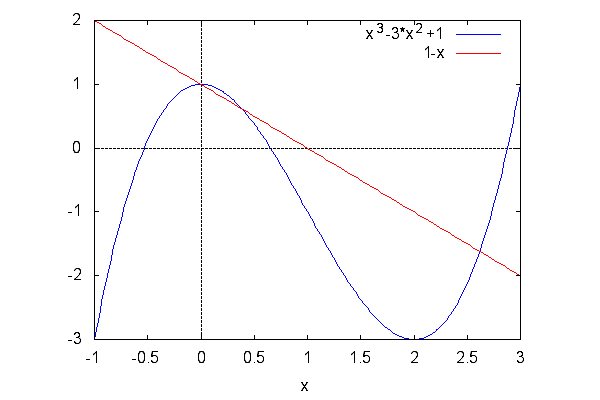
\includegraphics[height=2.6in,width=4.5in]{VOLUMEN_1/01_Vectores_Cartesianos/Figuras/Figura1_9aMax}
\end{center}
\end{figure}
\newline

Calculemos los puntos donde se interceptan las curvas:

%%%%%% INPUT:
\begin{minipage}[t]{8ex}
{\color{red}\bf \begin{verbatim} (%i20) 
\end{verbatim}}
\end{minipage}
\begin{minipage}[t]{\textwidth}{\color{blue}
\begin{verbatim}
solve(f(x)-g(x),x);
\end{verbatim}}
\end{minipage}

%%% OUTPUT:
\begin{math}\displaystyle \parbox{8ex}{\color{labelcolor}(\%o20) }
\left[ x=-\frac{\sqrt{5}-3}{2} , x=\frac{\sqrt{5}+3}{2} , x=0 \right] 
\end{math}
\newline

Los valores num�ricos son:

%%%%%% INPUT:
\begin{minipage}[t]{8ex}
{\color{red}\bf \begin{verbatim} (%i21) 
\end{verbatim}}
\end{minipage}
\begin{minipage}[t]{\textwidth}{\color{blue}
\begin{verbatim}
float(%);
\end{verbatim}}
\end{minipage}

%%% OUTPUT:
\begin{math}\displaystyle \parbox{8ex}{\color{labelcolor}(\%o21) }
\left[ x=0.3819660112501051 , x=2.618033988749895 , x=0.0 \right] 
\end{math}
\newline

Procedemos ahora s� a integrar la funci�n diferencia para encontrar el �rea contenida dentro de las dos funciones. En este caso ser� la integral:
\[
A=\int_{0}^{-\frac{\sqrt{5}-3}{2}} d(x) \ \mathrm{d}x + 
\int_{-\frac{\sqrt{5}-3}{2}}^{\frac{\sqrt{5}-3}{2}} (-d(x)) \ \mathrm{d}x \,.
\]

%%%%%% INPUT:
\begin{minipage}[t]{8ex}
{\color{red}\bf \begin{verbatim} (%i22) 
\end{verbatim}}
\end{minipage}
\begin{minipage}[t]{\textwidth}{\color{blue}
\begin{verbatim}
integrate(d(x),x,0,-(sqrt(5)-3)/2)+integrate(-d(x),x,-(sqrt(5)-3)/2,(sqrt(5)+3)/2);
\end{verbatim}}
\end{minipage}

%%% OUTPUT:
\begin{math}\displaystyle \parbox{8ex}{\color{labelcolor}(\%o22) }
\frac{5^{\frac{3}{2}}+11}{8}+\frac{5^{\frac{3}{2}}-11}{4}
\end{math}

%%%%%% INPUT:
\begin{minipage}[t]{8ex}
{\color{red}\bf \begin{verbatim} (%i23) 
\end{verbatim}}
\end{minipage}
\begin{minipage}[t]{\textwidth}{\color{blue}
\begin{verbatim}
float(%);
\end{verbatim}}
\end{minipage}

%%% OUTPUT:
\begin{math}\displaystyle \parbox{8ex}{\color{labelcolor}(\%o23) }
2.817627457812107
\end{math}
\newline

\item Calculemos ahora las dos integrales que aparecen en el ejemplo 8 de \ref{EjemDerVectores}. Es decir las integrales:
\[
\int_{\left(0,0\right)}^{\left(1,\frac{3}{4}\sqrt{2}\right)}
\left(3x^{2}+2xy^{3}\right)  \ \mathrm{d}x \,,\qquad 
\int_{\left(0,0\right)}^{\left(1,\frac{3}{4}\sqrt{2}\right)}6xy\ \mathrm{d}y\,.
\]
donde hicimos los cambio de variables: $
x=2\tau^{2}\,,\,\, y=\tau^{3}+\tau \,\, \Rightarrow \,\,
\mathrm{d}x =4\tau \mathrm{d}\tau \,, \,\,
\mathrm{d}y=(3\tau^{2}+1) \mathrm{d}\tau \,.
$

Escribiremos primero los dos integrandos:

%%%%%% INPUT:
\begin{minipage}[t]{8ex}
{\color{red}\bf \begin{verbatim} (%i24) 
\end{verbatim}}
\end{minipage}
\begin{minipage}[t]{\textwidth}{\color{blue}
\begin{verbatim}
int1:(3*x^2+2*x*y^3)*dx; int2:6*x*y*dy;
\end{verbatim}}
\end{minipage}

%%% OUTPUT:
\begin{math}\displaystyle \parbox{8ex}{\color{labelcolor}(\%o24) }
{\it dx}\,\left(2\,x\,y^3+3\,x^2\right)
\end{math}

%%% OUTPUT:
\begin{math}\displaystyle \parbox{8ex}{\color{labelcolor}(\%o25) }
6\,{\it dy}\,x\,y
\end{math}
\newline

Realizaremos el cambio de variable a trav�s de comando {\bf subst} que nos permite sustituir expresiones dentro de otras:

%%%%%% INPUT:
\begin{minipage}[t]{8ex}
{\color{red}\bf \begin{verbatim} (%i26) 
\end{verbatim}}
\end{minipage}
\begin{minipage}[t]{\textwidth}{\color{blue}
\begin{verbatim}
e1:subst([x=2*t^2,dx=4*t,y=t^3+t,dy=3*t^2+1],int1);
\end{verbatim}}
\end{minipage}

%%% OUTPUT:
\begin{math}\displaystyle \parbox{8ex}{\color{labelcolor}(\%o26) }
4\,t\,\left(4\,t^2\,\left(t^3+t\right)^3+12\,t^4\right)
\end{math}

%%%%%% INPUT:
\begin{minipage}[t]{8ex}
{\color{red}\bf \begin{verbatim} (%i27) 
\end{verbatim}}
\end{minipage}
\begin{minipage}[t]{\textwidth}{\color{blue}
\begin{verbatim}
e2:subst([x=2*t^2,dx=4*t,y=t^3+t,dy=3*t^2+1],int2);
\end{verbatim}}
\end{minipage}

%%% OUTPUT:
\begin{math}\displaystyle \parbox{8ex}{\color{labelcolor}(\%o27) }
12\,t^2\,\left(3\,t^2+1\right)\,\left(t^3+t\right)
\end{math}
\newline

Podemos introducir las integrales sin evaluarlas en el momento, esto se consigue mediante el operador de comilla simple. En este caso la funci�n no es evaluada y devuelve una expresi�n simb�lica o imagen pict�rica. 

%%%%%% INPUT:
\begin{minipage}[t]{8ex}
{\color{red}\bf \begin{verbatim} (%i28) 
\end{verbatim}}
\end{minipage}
\begin{minipage}[t]{\textwidth}{\color{blue}
\begin{verbatim}
int1:'integrate(e1,t,0,sqrt(2)/2);
\end{verbatim}}
\end{minipage}

%%% OUTPUT:
\begin{math}\displaystyle \parbox{8ex}{\color{labelcolor}(\%o28) }
4\,\int_{0}^{\frac{1}{\sqrt{2}}}{t\,\left(4\,t^2\,\left(t^3+t
 \right)^3+12\,t^4\right)\;dt}
\end{math}
\newline

Ahora si evaluamos la integral:

%%%%%% INPUT:
\begin{minipage}[t]{8ex}
{\color{red}\bf \begin{verbatim} (%i29) 
\end{verbatim}}
\end{minipage}
\begin{minipage}[t]{\textwidth}{\color{blue}
\begin{verbatim}
ev(int1,integrate),expand;
\end{verbatim}}
\end{minipage}

%%% OUTPUT:
\begin{math}\displaystyle \parbox{8ex}{\color{labelcolor}(\%o29) }
\frac{9305}{3003\,2^{\frac{5}{2}}}+1
\end{math}
\newline

Y para la segunda integral:

%%%%%% INPUT:
\begin{minipage}[t]{8ex}
{\color{red}\bf \begin{verbatim} (%i30) 
\end{verbatim}}
\end{minipage}
\begin{minipage}[t]{\textwidth}{\color{blue}
\begin{verbatim}
int2:'integrate(e2,t,0,sqrt(2)/2);
\end{verbatim}}
\end{minipage}

%%% OUTPUT:
\begin{math}\displaystyle \parbox{8ex}{\color{labelcolor}(\%o30) }
12\,\int_{0}^{\frac{1}{\sqrt{2}}}{t^2\,\left(3\,t^2+1\right)\,
 \left(t^3+t\right)\;dt}
\end{math}

%%%%%% INPUT:
\begin{minipage}[t]{8ex}
{\color{red}\bf \begin{verbatim} (%i31) 
\end{verbatim}}
\end{minipage}
\begin{minipage}[t]{\textwidth}{\color{blue}
\begin{verbatim}
ev(int2,integrate),expand;
\end{verbatim}}
\end{minipage}

%%% OUTPUT:
\begin{math}\displaystyle \parbox{8ex}{\color{labelcolor}(\%o31) }
\frac{65}{32}
\end{math}

%%%%%% INPUT:
\begin{minipage}[t]{8ex}
{\color{red}\bf \begin{verbatim} (%i32) 
\end{verbatim}}
\end{minipage}
\begin{minipage}[t]{\textwidth}{\color{blue}
\begin{verbatim}
kill(all)$
\end{verbatim}}
\end{minipage}
\newline

\item Para finalizar, aclaremos la diferencia entre asignar  una expresi�n a una variable y la definici�n de funciones. 
Consideremos el movimiento de una part�cula que sigue la trayectoria: 
\[
x=x_0+v_0 t +\frac12 at^2 \,.
\]

Primero escribiremos la expresi�n y se la asignamos a una variable que llamaremos $x$.

%%%%%% INPUT:
\begin{minipage}[t]{8ex}
{\color{red}\bf \begin{verbatim} (%i1) 
\end{verbatim}}
\end{minipage}
\begin{minipage}[t]{\textwidth}{\color{blue}
\begin{verbatim}
x:x0+v0*t+a*t^2/2;
\end{verbatim}}
\end{minipage}

%%% OUTPUT:
\begin{math}\displaystyle \parbox{8ex}{\color{labelcolor}(\%o1) }
{ x_0}+t\,{v_0}+\frac{a\,t^2}{2}
\end{math}
\newline

Si queremos evaluarla para alg�n valor de la variable $t$, digamos $t=1$, entonces podemos escribir:

%%%%%% INPUT:
\begin{minipage}[t]{8ex}
{\color{red}\bf \begin{verbatim} (%i2) 
\end{verbatim}}
\end{minipage}
\begin{minipage}[t]{\textwidth}{\color{blue}
\begin{verbatim}
subst(t=1,x);
\end{verbatim}}
\end{minipage}

%%% OUTPUT:
\begin{math}\displaystyle \parbox{8ex}{\color{labelcolor}(\%o2) }
{ x_0}+{ v_0}+\frac{a}{2}
\end{math}
\newline

Si queremos evaluar la expresi�n con el resto de par�metros, entonces:

%%%%%% INPUT:
\begin{minipage}[t]{8ex}
{\color{red}\bf \begin{verbatim} (%i3) 
\end{verbatim}}
\end{minipage}
\begin{minipage}[t]{\textwidth}{\color{blue}
\begin{verbatim}
subst([t=1,a=-9.8,x0=0,v0=10],x);
\end{verbatim}}
\end{minipage}

%%% OUTPUT:
\begin{math}\displaystyle \parbox{8ex}{\color{labelcolor}(\%o3) }
5.1
\end{math}
\newline

Las sustituciones se realizan pero no se asignan a las variables.  Podemos ver que $x$ sigue siendo lo que le asignamos originalmente.

%%%%%% INPUT:
\begin{minipage}[t]{8ex}
{\color{red}\bf \begin{verbatim} (%i4) 
\end{verbatim}}
\end{minipage}
\begin{minipage}[t]{\textwidth}{\color{blue}
\begin{verbatim}
x;
\end{verbatim}}
\end{minipage}

%%% OUTPUT:
\begin{math}\displaystyle \parbox{8ex}{\color{labelcolor}(\%o4) }
{ x_0}+t\,{ v_0}+\frac{a\,t^2}{2}
\end{math}
\newline

Ahora definamos la expresi�n anterior pero como la funci�n $x(t)$.

%%%%%% INPUT:
\begin{minipage}[t]{8ex}
{\color{red}\bf \begin{verbatim} (%i5) 
\end{verbatim}}
\end{minipage}
\begin{minipage}[t]{\textwidth}{\color{blue}
\begin{verbatim}
x(t):=x0+v0*t+a*t^2/2;
\end{verbatim}}
\end{minipage}

%%% OUTPUT:
\begin{math}\displaystyle \parbox{8ex}{\color{labelcolor}(\%o5) }
x(t):=x_0+v_0 t+a \frac{t^2}{2}
\end{math}
\newline

Evaluarla es ahora m�s sencillo:

%%%%%% INPUT:
\begin{minipage}[t]{8ex}
{\color{red}\bf \begin{verbatim} (%i6) 
\end{verbatim}}
\end{minipage}
\begin{minipage}[t]{\textwidth}{\color{blue}
\begin{verbatim}
x(1);
\end{verbatim}}
\end{minipage}

%%% OUTPUT:
\begin{math}\displaystyle \parbox{8ex}{\color{labelcolor}(\%o6) }
{ x_0}+{ v_0}+\frac{a}{2}
\end{math}
\newline

Tambi�n podemos escribir:

%%%%%% INPUT:
\begin{minipage}[t]{8ex}
{\color{red}\bf \begin{verbatim} (%i7) 
\end{verbatim}}
\end{minipage}
\begin{minipage}[t]{\textwidth}{\color{blue}
\begin{verbatim}
subst([a=-9.8,x0=0,v0=10],x(1));
\end{verbatim}}
\end{minipage}

%%% OUTPUT:
\begin{math}\displaystyle \parbox{8ex}{\color{labelcolor}(\%o7) }
5.1
\end{math}
\newline

Si queremos asignarle los valores a los par�metros de manera global, entonces escribimos:

%%%%%% INPUT:
\begin{minipage}[t]{8ex}
{\color{red}\bf \begin{verbatim} (%i8) 
\end{verbatim}}
\end{minipage}
\begin{minipage}[t]{\textwidth}{\color{blue}
\begin{verbatim}
a:-9.8$ x0:0$ v0:10$
\end{verbatim}}
\end{minipage}
\newline

De manera que:

%%%%%% INPUT:
\begin{minipage}[t]{8ex}
{\color{red}\bf \begin{verbatim} (%i11) 
\end{verbatim}}
\end{minipage}
\begin{minipage}[t]{\textwidth}{\color{blue}
\begin{verbatim}
x(1);
\end{verbatim}}
\end{minipage}

%%% OUTPUT:
\begin{math}\displaystyle \parbox{8ex}{\color{labelcolor}(\%o11) }
5.1
\end{math}
\newline

Para limpiar los par�metros que acabamos de asignar hacemos lo siguiente:

%%%%%% INPUT:
\begin{minipage}[t]{8ex}
{\color{red}\bf \begin{verbatim} (%i12) 
\end{verbatim}}
\end{minipage}
\begin{minipage}[t]{\textwidth}{\color{blue}
\begin{verbatim}
kill(a,v0,x0)$
\end{verbatim}}
\end{minipage}
\newline

Por lo tanto:

%%%%%% INPUT:
\begin{minipage}[t]{8ex}
{\color{red}\bf \begin{verbatim} (%i13) 
\end{verbatim}}
\end{minipage}
\begin{minipage}[t]{\textwidth}{\color{blue}
\begin{verbatim}
x(1);
\end{verbatim}}
\end{minipage}

%%% OUTPUT:
\begin{math}\displaystyle \parbox{8ex}{\color{labelcolor}(\%o13) }
{ x_0}+{ v_0}+\frac{a}{2}
\end{math}
\newline

La velocidad y la aceleraci�n son funciones f�ciles de calcular:

%%%%%% INPUT:
\begin{minipage}[t]{8ex}
{\color{red}\bf \begin{verbatim} (%i14) 
\end{verbatim}}
\end{minipage}
\begin{minipage}[t]{\textwidth}{\color{blue}
\begin{verbatim}
'diff(x(t),t)=diff(x(t),t);
\end{verbatim}}
\end{minipage}

%%% OUTPUT:
\begin{math}\displaystyle \parbox{8ex}{\color{labelcolor}(\%o14) }
\frac{d}{d\,t}\,\left({ x_0}+t\,{ v_0}+\frac{a\,t^2}{2}
 \right)={ v_0}+a\,t
\end{math}

%%%%%% INPUT:
\begin{minipage}[t]{8ex}
{\color{red}\bf \begin{verbatim} (%i15) 
\end{verbatim}}
\end{minipage}
\begin{minipage}[t]{\textwidth}{\color{blue}
\begin{verbatim}
'diff(x(t),t,2)=diff(x(t),t,2);
\end{verbatim}}
\end{minipage}

%%% OUTPUT:
\begin{math}\displaystyle \parbox{8ex}{\color{labelcolor}(\%o15) }
\frac{d^2}{d\,t^2}\,\left({ x_0}+t\,{ v_0}+\frac{a\,t^2}{2} \right)=a
\end{math}
\newline

En el caso de que estemos interesados en definir una nueva funci�n a partir de alg�n c�lculo anterior podemos utilizar la funci�n  {\bf define}. 

Entonces, lo que vamos a hacer, en las siguientes lineas de comandos, es definir la funci�n velocidad a partir de la derivada de la posici�n. 

%%%%%% INPUT:
\begin{minipage}[t]{8ex}
{\color{red}\bf \begin{verbatim} (%i16) 
\end{verbatim}}
\end{minipage}
\begin{minipage}[t]{\textwidth}{\color{blue}
\begin{verbatim}
diff(x(t),t);
\end{verbatim}}
\end{minipage}

%%% OUTPUT:
\begin{math}\displaystyle \parbox{8ex}{\color{labelcolor}(\%o16) }
{v_0}+a\,t
\end{math}

%%%%%% INPUT:
\begin{minipage}[t]{8ex}
{\color{red}\bf \begin{verbatim} (%i17) 
\end{verbatim}}
\end{minipage}
\begin{minipage}[t]{\textwidth}{\color{blue}
\begin{verbatim}
define(v(t),%);
\end{verbatim}}
\end{minipage}

%%% OUTPUT:
\begin{math}\displaystyle \parbox{8ex}{\color{labelcolor}(\%o17) }
v(t):=v0+at
\end{math}

%%%%%% INPUT:
\begin{minipage}[t]{8ex}
{\color{red}\bf \begin{verbatim} (%i18) 
\end{verbatim}}
\end{minipage}
\begin{minipage}[t]{\textwidth}{\color{blue}
\begin{verbatim}
v(1);
\end{verbatim}}
\end{minipage}

%%% OUTPUT:
\begin{math}\displaystyle \parbox{8ex}{\color{labelcolor}(\%o18) }
v0+a
\end{math}

%%%%%% INPUT:
\begin{minipage}[t]{8ex}
{\color{red}\bf \begin{verbatim} (%i19) 
\end{verbatim}}
\end{minipage}
\begin{minipage}[t]{\textwidth}{\color{blue}
\begin{verbatim}
subst([a=-9.8,x0=0,v0=10],v(1));
\end{verbatim}}
\end{minipage}

%%% OUTPUT:
\begin{math}\displaystyle \parbox{8ex}{\color{labelcolor}(\%o19) }
0.1999999999999993
\end{math}
\newline

\item Cuando necesitemos manejar campo vectoriales podemos utilizar las listas. Veamos el primer ejemplo de \ref{EjemDerVectores} donde:
\[ 
{\bf r}=3t^2 {\bf i}+(4t^3-t){\bf j}+t{\bf k} \,.
\]

Escribamos el vector posici�n:

%%%%%% INPUT:
\begin{minipage}[t]{8ex}
{\color{red}\bf \begin{verbatim} (%i20) 
\end{verbatim}}
\end{minipage}
\begin{minipage}[t]{\textwidth}{\color{blue}
\begin{verbatim}
[x,y,z]:[3*t^2,4*t^3-t,t];
\end{verbatim}}
\end{minipage}

%%% OUTPUT:
\begin{math}\displaystyle \parbox{8ex}{\color{labelcolor}(\%o20) }
\left[ 3\,t^2 , 4\,t^3-t , t \right]
\end{math}
\newline

La velocidad:

%%%%%% INPUT:
\begin{minipage}[t]{8ex}
{\color{red}\bf \begin{verbatim} (%i21) 
\end{verbatim}}
\end{minipage}
\begin{minipage}[t]{\textwidth}{\color{blue}
\begin{verbatim}
v:diff([x,y,z],t);
\end{verbatim}}
\end{minipage}

%%% OUTPUT:
\begin{math}\displaystyle \parbox{8ex}{\color{labelcolor}(\%o21) }
\left[ 6\,t , 12\,t^2-1 , 1 \right] 
\end{math}
\newline

La aceleraci�n:

%%%%%% INPUT:
\begin{minipage}[t]{8ex}
{\color{red}\bf \begin{verbatim} (%i22) 
\end{verbatim}}
\end{minipage}
\begin{minipage}[t]{\textwidth}{\color{blue}
\begin{verbatim}
a:diff([x,y,z],t,2);
\end{verbatim}}
\end{minipage}

%%% OUTPUT:
\begin{math}\displaystyle \parbox{8ex}{\color{labelcolor}(\%o22) }
\left[ 6 , 24\,t , 0 \right]
\end{math}
\newline

Podemos facilmente calcular: 

%%%%%% INPUT:
\begin{minipage}[t]{8ex}
{\color{red}\bf \begin{verbatim} (%i23) 
\end{verbatim}}
\end{minipage}
\begin{minipage}[t]{\textwidth}{\color{blue}
\begin{verbatim}
v.[bx,by,bz];
\end{verbatim}}
\end{minipage}

%%% OUTPUT:
\begin{math}\displaystyle \parbox{8ex}{\color{labelcolor}(\%o23) }
{ by}\,\left(12\,t^2-1\right)+6\,{ bx}\,t+{ bz}
\end{math}

%%%%%% INPUT:
\begin{minipage}[t]{8ex}
{\color{red}\bf \begin{verbatim} (%i24) 
\end{verbatim}}
\end{minipage}
\begin{minipage}[t]{\textwidth}{\color{blue}
\begin{verbatim}
solve(%,bz);
\end{verbatim}}
\end{minipage}

%%% OUTPUT:
\begin{math}\displaystyle \parbox{8ex}{\color{labelcolor}(\%o24) }
\left[ { bz}=-12\,{ by}\,t^2-6\,{ bx}\,t+{ by} \right] 
\end{math}

\end{enumerate}

\begin{center}
{\color{red}\rule{15.8cm}{0.4mm}}
\end{center}


\subsection{{\color{OliveGreen}Ejercicios}}
\begin{enumerate}
\item Demuestre que:
\begin{enumerate}
\item 
$
\frac{\mathrm{d}}{\mathrm{d} t}\left[ \mathbf{a} \cdot \left( \mathbf{b}\times \mathbf{c} \right) \right] = 
 \frac{\mathrm{d}\mathbf{a} }{\mathrm{d} t}\cdot\left( \mathbf{b}\times \mathbf{c} \right)  + \mathbf{a}\cdot \left( \frac{\mathrm{d}\mathbf{b} }{\mathrm{d} t}\times \mathbf{c} \right) +\mathbf{a}\cdot \left(\mathbf{b} \times \frac{\mathrm{d}\mathbf{c} }{\mathrm{d} t} \right)
$
\item 
$
\frac{\mathrm{d}}{\mathrm{d} t}\left[ \mathbf{a} \cdot \left( \frac{\mathrm{d}\mathbf{a} }{\mathrm{d} t}\times 
\frac{\mathrm{d}^2\mathbf{a} }{\mathrm{d} t^2}  \right) \right] = 
\mathbf{a}\cdot \left( \frac{\mathrm{d}\mathbf{a} }{\mathrm{d} t}\times 
\frac{\mathrm{d}^3\mathbf{a} }{\mathrm{d} t^3}  \right) 
$
\item 
$
{\boldsymbol \nabla}\times ({\boldsymbol \nabla}\times {\bf a}) =
{\boldsymbol \nabla}{\boldsymbol \nabla}\cdot {\bf a}-
{\boldsymbol \nabla}\cdot {\boldsymbol \nabla}{\bf a}
$
\item 
$
{\boldsymbol \nabla}\times (\phi{\boldsymbol \nabla}\phi)=0
$
\item 
$
{\boldsymbol \nabla}\times [ {\bf a}\times
({\boldsymbol \nabla}\times {\bf a})]=0
$, si $ {\bf a}= a_x(y,z){\bf i}$.
\end{enumerate}

\item Considere que: 
   \begin{itemize}
  \item ${\bf r}  =x\ \mathbf{{\bf i}}+y\ \mathbf{{\bf j}}+z\ \mathbf{{\bf k}}= x^{i}\mathbf{{i}}_{i}$,
  \item ${\bf a} = {\bf a}({\bf r}) = {\bf a}(x,y,z) = a^{i}(x,y,z) {\bf i}_{i} \,\, $  \mbox{y} $ {\bf b} = {\bf b}({\bf r}) =  {\bf b}(x,y,z) = b^{i}(x,y,z) {\mathbf{{i}}}_{i}$,
  \item $\phi = \phi({\bf r}) = \phi(x,y,z) \quad$ y $\,\, \psi = \psi({\bf r}) = \psi(x,y,z)$. 
\end{itemize} 

Utilizando la notaci�n de �ndices, e inspir�ndose en las secciones: \ref{ParCalculos}, \ref{VectorGradiente} y \ref{EjemDerVectores}, demuestre las siguientes identidades vectoriales: 
  \begin{enumerate}
  \item ${\boldsymbol \nabla}(\phi \psi) = \phi {\boldsymbol \nabla}\psi + \psi {\boldsymbol \nabla}\phi$.
  \item ${\boldsymbol \nabla} \cdot (\phi {\bf a}) = \phi {\boldsymbol \nabla} \cdot {\bf a}  + ({\boldsymbol \nabla}\phi)  \cdot {\bf a} $.
  \item ${\boldsymbol \nabla} \times {\boldsymbol \nabla}\phi = 0 $.
  \item $ {\boldsymbol \nabla} \cdot ({\boldsymbol \nabla} \times {\bf a})$  �Qu� puede decir de $ {\boldsymbol \nabla} \times ({\boldsymbol \nabla}  \cdot {\bf a})$?
  \item ${\boldsymbol \nabla} \cdot ( {\bf a} \times {\bf b}) = ({\boldsymbol \nabla}  \times {\bf a})  \cdot {\bf b} -   {\bf a} \cdot  ({\boldsymbol \nabla}  \times {\bf b})$.
  \item ${\boldsymbol \nabla} \times ( {\boldsymbol \nabla} \times  {\bf a} ) = {\boldsymbol \nabla}(  {\boldsymbol \nabla}  \cdot {\bf a} ) - {\boldsymbol \nabla}^{2} {\bf a} $ .   
\end{enumerate}

\item Para los vectores dados a continuaci�n, encuentre $d{\bf r}/ds$
\begin{enumerate}
\item ${\bf r} = t{\bf i}+3t^2{\bf j}-(t -1){\bf k}$, y $t = \ln(1+s^2)$.
\item ${\bf r} = \mbox{sen}(t){\bf i}+\cos(t){\bf j}+\tan(t){\bf k}$,  y $t = 2+s^2$.
\end{enumerate}

\item Una part�cula describe un movimiento dado por el vector posici�n ${\bf r}$. Encuentre la componente de su velocidad en la direcci�n del vector indicado:
\begin{enumerate}
\item ${\bf r} = t^2{\bf i}+4\cos(2t){\bf j}+3\mbox{sen}(2t){\bf k},\quad$  
$2{\bf i}+{\bf j}+2{\bf k}$.
\item ${\bf r} = 3\cos(t){\bf i}+3\mbox{sen}(t){\bf j}+(t^2-2){\bf k},\quad$   
${\bf i}+2{\bf j}-{\bf k}$.
\end{enumerate}

\item Si {\bf u}, {\bf v} y {\bf w} son funciones que dependen del par�metro $t$, demuestre que:
\begin{enumerate}
\item 
$\frac{\mathrm{d}}{\mathrm{d}t}\left[{\bf u}\cdot({\bf v}\times{\bf w})\right] ={\bf u}\cdot \left({\bf v}\times \frac{\mathrm{d}{\bf w}}{\mathrm{d}t} \right)+{\bf u}\cdot \left(\frac{\mathrm{d}{\bf v}}{\mathrm{d}t}\times {\bf w} \right)+\frac{\mathrm{d}{\bf u}}{\mathrm{d}t}\cdot({\bf v}\times{\bf w})$.  
\item $\frac{\mathrm{d}}{\mathrm{d}t}\left[{\bf u}\times({\bf v}\times{\bf w})\right] ={\bf u}\times \left({\bf v}\times \frac{\mathrm{d}{\bf w}}{\mathrm{d}t} \right)+{\bf u}\times \left(\frac{\mathrm{d}{\bf v}}{\mathrm{d}t}\times {\bf w} \right)+\frac{\mathrm{d}{\bf u}}{\mathrm{d}t}\times({\bf v}\times{\bf w})$.
\end{enumerate}

\item Si ${\bf u} = 2t{\bf i}-t^2{\bf j}+{\bf k}$, ${\bf v}= 2{\bf i}+3t{\bf j}+t{\bf k}$ y ${\bf w} = t{\bf i}+2t{\bf j}-t{\bf k}$. Utilice el resultado del ejercicio (a) anterior para encontrar: $\frac{\mathrm{d}}{\mathrm{d}t}\left[{\bf u}\cdot({\bf v}\times{\bf w})\right]$.

\item Si ${\bf u} = t{\bf i}-t{\bf j}+t^2{\bf k}$, ${\bf v}= -t{\bf i}+2t{\bf j}-t^2{\bf k}$ y ${\bf w} = 2t{\bf i}-2t{\bf j}+t{\bf k}$. Utilice el resultado del ejercicio (b) anterior para encontrar: $\frac{\mathrm{d}}{\mathrm{d}t}\left[{\bf u}\times({\bf v}\times{\bf w})\right]$.


\item Encuentre el gradiente de los siguientes campos:
\begin{enumerate}
\item $\phi(x,y,z)= x^2+3xyz-yz^2 $.
\item $\phi(x,y,z)= \left(x^2 + 2y^2 + 4z^2\right)^{-1} $.
\end{enumerate}

\item Encuentre la divergencia de los siguientes campos:
\begin{enumerate}
\item ${\bf a} (x,y,z)=x^2y{\bf i}+y^2z^2{\bf j}+xz^3{\bf k} $.
\item ${\bf a} (x,y,z)=(1-x^2){\bf i}+\mbox{sen}(yz){\bf j}+e^{xyz}{\bf k}$.
\end{enumerate}

\item Encuentre el rotor de los siguientes campos:
\begin{enumerate}
\item ${\bf a} (x,y,z)=xyz^2{\bf i}+x^2yz{\bf j}+xy^2{\bf k} $.
\item ${\bf a} (x,y,z)=\mbox{senh}(xy){\bf i}+\cosh(yz){\bf j}+xyz{\bf k} $.
\end{enumerate}

\item Eval�e las siguientes integrales:
\begin{enumerate}
\item $\int \left(t \mbox{sen}(t){\bf i}+2t^2{\bf j}-7t{\bf k}\right) \mathrm{d}t$.
\item $\int \left( \mbox{cosh}^2(t){\bf i}+2\mbox{sen}^2(2t){\bf j}-{\bf k}\right) \mathrm{d}t$.
\end{enumerate}


\item Un campo de fuerza: 
\[
{\bf F}= -kx{\bf i}-ky{\bf j} \,,
\]
act�a sobre un oscilador.  Compare el trabajo hecho al moverse en contra de este campo al ir desde el punto $(1,1)$ al punto $(4,4)$, siguiendo los siguientes caminos:
\[
{a)} \,\, (1,1) \rightarrow (4,1) \rightarrow (4,4).\quad 
{b)} \,\, (1,1) \rightarrow (1,4) \rightarrow (4,4).\quad 
{c)} \,\, (1,1) \rightarrow (4,4), \,\, \mbox{siguiendo el camino:}  \,\, x=y.
\]

\item Dado el campo de fuerza:  
\[
{\bf F}= -\frac{y}{x^2+y^2}{\bf i}+\frac{x}{x^2+y^2}{\bf j}\,. 
\]
Calcule el trabajo hecho en contra de este campo de fuerza  al moverse al rededor de un circulo de radio uno y en el plano $x-y$.
\begin{enumerate}
\item desde $0$ a $\pi$ en sentido contrario a la agujas del reloj.
\item desde $0$ a $-\pi$ en sentido de las agujas del reloj. 
\end{enumerate}

\item Evaluar la siguiente integral:
\[
\oint {\bf r}\cdot \mathrm{d}{\bf r}\,.
\]

 \item Una part�cula se mueve bajo la ley ${\bf r}(t) = x(t){\bf i} + y(t){\bf j} +z(t){\bf k}$, con: 
 \[
 x(t) = 2t^{2}; \quad  y(t) = t^{2} -4t; \quad  z(t) = 3t -5.
 \]
El par�metro $t$ representa el tiempo. 

Encuentre las expresiones para la aceleraci�n y la velocidad de la part�cula, para $t=1$ y en la direcci�n del vector ${\bf i} -3{\bf j}+2{\bf k}$. 

\item Suponga ahora el caso general de una part�cula que se mueve en una curva descrita por: 
\[
{\bf r}(t) = x(t){\bf i} + y(t){\bf j} +z(t){\bf k}\,.
\]
Muestre que el vector velocidad es tangente a la trayectoria descrita. 
 
 \item Encuentre la ecuaci�n vectorial para una trayectoria recta que pasa por los puntos $P \rightarrow (1, 2, 3)$ y $Q \rightarrow (1, 1, 1)$.

\item Encuentre el �ngulo entre los siguientes planos: $x + y +z = 9$ y  $x + y -z = 3$.  

\item Un fluido se considera irrotacional si su campo de velocidades ${\bf v}={\bf v}({\bf r}) ={\bf v}(x,y,z)$ cumple con la  ecuaci�n: $ {\boldsymbol \nabla} \times  {\bf v} =0$. Suponga, ahora que: ${\bf v} = (x +2y +az){\bf i} +(bx -3y -z){\bf j} +(4x +cy +2z){\bf k}$.
 \begin{enumerate}
  \item Encuentre el valor de $a, b$ y $c$ para que este campo de velocidades sea irrotacional.
  
  \item Es intuitivo convencerse que si $ {\boldsymbol \nabla} \times  {\bf v} =0 \,\, \Rightarrow \,\, {\bf v} = {\boldsymbol \nabla} \psi $. Encuentre la expresi�n para la funci�n potencial $ \psi = \psi({\bf r}) = \psi(x,y,z)$.
  
  \item Considere la siguiente integral: $I = \int_{\mathcal{C}} \; \mathrm{d} {\bf r} \cdot {\bf v}$. Donde $\mathcal{C}$ es el circuito a recorrer. 
  \begin{enumerate}
  \item Calcule el valor de la integral $I$ a lo largo del  trayecto: $(0,0,0) \rightarrow (1,1,0)$ mediante una segmento de recta. Luego, de $ (1,1,0) \rightarrow (2,0,0)$ a lo largo de otro segmento de recta. Finalmente regresando $(2,0,0) \rightarrow (0,0,0)$ tambi�n siguiendo una recta.
  \item Calcule el valor de la integral $I$ de $ (0,0,0) \rightarrow (2,0,0)$ a lo largo de un arco de circunferencia que cumple con la ecuaci�n: $(x-1)^{2} + y^{2} =1$. Ahora regresando de $(2,0,0) \rightarrow (0,0,0)$ tambi�n a trav�s de una recta.
  \item �Qu� puede concluir del campo ${\bf v}$?
\end{enumerate}
\end{enumerate}

\item Resuelva todos los problemas anteriores utilizando {\bf Maxima}.

\end{enumerate}

\section{Vectores y n�meros complejos}
\label{VectoresNumerosComplejos}
\index{N�meros complejos!Vectores 2D}
\index{Vectores 2D!N�meros complejos}
Desde los primeros cursos de matem�tica nos hemos tropezado con las llamadas ra�ces imaginarias o complejas de
polinomios. La soluci�n a un polinomio c�bico: 
\[
x^{3}-3x^{2}+4x-12=0\,\, \Rightarrow \,\,  \left\{
\begin{array}
[c]{c}
x=2i\\
x=-2i\\
x=3
\end{array}
\right\}  \,\, \Rightarrow \,\,  \left(  x+2i\right)  \left(  x-2i\right)
\left(  x-3\right)  =0 \,,
\]
o cuadr�tico:
\[
x^{2}+4=0\,\, \Rightarrow \,\,   \left\{
\begin{array}
[c]{c}
x=2i\\
x=-2i
\end{array}
\right\} \,\, \Rightarrow \,\,  \left( x+2i\right)  \left(  x-2i\right)=0\,.
\]
nos lleva a definir un n�mero $i^{2}\equiv-1$. 

De lo anterior podemos ver que al multiplicar el n�mero imaginario $i$ por cualquier n�mero real obtendremos el n�mero imaginario puro  $i b$, con $b \in \mathds{R}$. La nomenclatura  de n�meros imaginarios surgi� de la idea de que estas cantidades no representaban mediciones f�sicas. Esa idea ha sido abandonada pero el nombre qued�\footnote{Los n�meros complejos comienzan a aparecer en los trabajos de Cardano (1501-1576) y Bombelli (1526-1672) mientras estudiaban las ra�ces de la ecuaci�n c�bica . Pero es a Ren� Descartes (1596-1650) a qui�n se le atribuye la afirmaci�n: ``ciertas ecuaciones algebraicas s�lo tienen soluci�n en nuestra imaginaci�n'' y utiliz� el t�rmino ``n�meros imaginarios''. 
Caspar Wessel en 1799 y Jean-Robert Argand en 1806 proponen la estructura del plano complejo y la representaci�n de la unidad imaginaria como el punto $(0,1)$ del eje vertical de dicho plano. Pero el t�rmino, hoy usado de ''n�meros complejos'' se debe a Johann Carl Friedrich Gauss (1777-1855).}.

Es importante se�alar aqu�, que suele tomarse de la definici�n $i^{2}\equiv-1$ que $i=\sqrt{-1}$. Pero si hacemos esto, sin pensarlo bien, llegamos a que: $-1=i^{2}=i i=\sqrt{-1}\sqrt{-1}=\sqrt{1}=1$. La contradicci�n surge por el hecho de que aqu� el $-1$ no es un n�mero real sino un n�mero complejo y ser� evidente m�s adelante cuando desarrollemos el algebra de los n�meros complejos.


\subsection{Los n�meros complejos y su �lgebra}
\label{NumerosComplejosAlgebra}
\index{N�meros complejos!�lgebra}
\index{�lgebra de n�meros complejos}
Un n�mero complejo, $z,$ es la generalizaci�n de los n�meros imaginarios (puros), $ib$. Esto es:
\[
z=a+ib\quad\quad\text{con }a,b \in \mathds{R} \,\,  \Rightarrow \,\,  
\left\{
\begin{array}
[c]{l}
a\rightarrow\quad\text{parte real}\\
b\rightarrow\quad\text{parte imaginaria}
\end{array}
\right.
\]

Obviamente los n�meros reales ser�n $a+i0$ n�meros complejos con su parte imaginaria nula. Los n�meros imaginarios puros ser�n n�meros complejos con su parte real nula, esto es, $0+ib.$ Por ello, en general diremos que:
\[
z=a+ib \,\,  \Rightarrow \,\, a=\operatorname{Re}\left(  z\right)  \quad
\wedge\quad b=\operatorname{Im}\left(  z\right)\,,
\]
es decir, $a$ corresponde a la parte real de $z$ y $b$ a su parte imaginaria. 

Cada n�mero complejo, $z$ tendr� asociado un n�mero complejo conjugado,
$z^{\ast}$ tal que:
\begin{gather*}
z=a+ib\quad\rightleftharpoons\quad z^{\ast}=a-ib \,, \\
\Downarrow\\
\left(  z^{\ast}\right)  ^{\ast}=z\quad\wedge\quad z\cdot z^{\ast}=a^{2}+b^{2}\,,
\end{gather*}
claramente:
\[
z\cdot z^{\ast}\geq0 \,\,  \Rightarrow \,\, \left|  z\right|  ^{2}=\left|
z^{\ast}\right|  ^{2}=z\cdot z^{\ast}=a^{2}+b^{2} \,.
\]

Es importante se�alar que, en general, no existe relaci�n de orden entre los n�meros complejos. Vale decir, que no sabremos si un n�mero complejo es mayor que otro. No est� definida esta operaci�n.
\[
z_{1}\ngtr z_{2}\quad\vee\quad z_{1}\nless z_{2} \,.
\]

Las relaciones de orden s�lo se podr�n establecer entre m�dulos de n�meros complejos y no n�meros complejos en general.

R�pidamente recordamos el �lgebra de los n�meros complejos:

\begin{itemize}
\item  Dos n�meros complejos ser�n iguales si sus partes reales e
imaginarios lo son:
\[
z_{1}=z_{2} \,\, \Rightarrow \,\, \left(  a_{1}+ib_{1}\right)  =\left(
a_{2}+ib_{2}\right)  \,\, \Rightarrow \,\, a_{1}=a_{2}\quad\wedge\quad
b_{1}=b_{2} \,.
\]

\item  Se suman dos n�meros complejos sumando sus partes reales y sus partes imaginarias:
\[
z_{3}=z_{1}+z_{2} \,\,  \Rightarrow \,\, \left(  a_{1}+ib_{1}\right)  +\left(
a_{2}+ib_{2}\right)  ={{\left( a_{1}+a_{2}\right)
}}+i{{\left(  b_{1}+b_{2}\right)  }}=a_{3}+ib_{3} \,,
\]
claramente $z+z^{\ast}=2\operatorname{Re}z$, tambi�n $z-z^{\ast
}=2\operatorname{Im}z.$ Igualmente es inmediato comprobar que:
\[
\left(  z_{1}+z_{2}\right)  ^{\ast}=z_{1}^{\ast}+z_{2}^{\ast}\,.
\]

\item  Se multiplican n�meros complejos por escalares multiplicando el escalar por sus partes reales e imaginarias:
\[
z_{3}=\alpha z_{1} \,\, \Rightarrow \,\, \alpha\left(  a_{1}+ib_{1}\right)
= \alpha a_{1}  +i\left(  \alpha b_{1}\right)\,.
\]

\item  Se multiplican n�meros complejos entre si, multiplicando los dos binomios y teniendo cuidado que $i^{2}=-1$:
\[
z_{3}=z_{1}z_{2}\,\, \Rightarrow \,\, \left(  a_{1}+ib_{1}\right)  \cdot\left(
a_{2}+ib_{2}\right)  =\left(  a_{1}a_{2}-b_{1}b_{2}\right)  +i\left(
a_{1}b_{2}+b_{1}a_{2}\right)\,,
\]
tambi�n es inmediato comprobar que $\left(  z_{1}z_{2}\right)  ^{\ast }=z_{1}^{\ast}z_{2}^{\ast}$.

\item  Se dividen n�meros complejos siguiendo la estrategia de
racionalizaci�n de fracciones irracionales. Esto es:
\[
z_{3}=\frac{z_{1}}{z_{2}} \,\, \Rightarrow \,\, \frac{\left(  a_{1}
+ib_{1}\right)  }{\left(  a_{2}+ib_{2}\right)  }=\frac{\left(  a_{1}
+ib_{1}\right)  }{\left(  a_{2}+ib_{2}\right)  }\frac{\left(  a_{2}
-ib_{2}\right)  }{\left(  a_{2}-ib_{2}\right)  }=\frac{a_{1}a_{2}+b_{1}b_{2}
}{\left(  a_{2}^{2}+b_{2}^{2}\right)  }+i\frac{b_{1}a_{2}-a_{1}b_{2}}{\left(
a_{2}^{2}+b_{2}^{2}\right)  }\,,
\]
es claro que el divisor ser� cualquier n�mero complejo excepto el cero complejo: $0+i0$.
\end{itemize}

\subsection{Vectores y el plano complejo}
Mirando con cuidado el �lgebra de n�meros complejos nos damos cuenta que un n�mero complejo puede ser representado por una \textit{dupla} de n�meros, es decir:
\[
z=\left( a+ib\right) \quad \leftrightharpoons \quad z=\left( a,b\right)\,.
\]

Las propiedades entre n�meros complejos de igualdad, suma y multiplicaci�n por un escalar arriba expuestas se cumplen de forma inmediata con esta nueva representaci�n. Hay que definir las operaciones de multiplicaci�n y
divisi�n entre n�meros complejos de forma que:
\[
\left( a_{1},b_{1}\right) \left( a_{2},b_{2}\right) =\left(
a_{1}a_{2}-b_{1}b_{2},a_{1}b_{2}+b_{1}a_{2}\right) \quad \wedge \quad \frac{
\left( a_{1},b_{1}\right) }{\left( a_{2},b_{2}\right) }=\left( \frac{
a_{1}a_{2}+b_{1}b_{2}}{\left( a_{2}^{2}+b_{2}^{2}\right) },\frac{
b_{1}a_{2}-a_{1}b_{2}}{\left( a_{2}^{2}+b_{2}^{2}\right) }\right)\,.
\]

Con est� definici�n para la multiplicaci�n de n�meros complejos podemos ver que si la unidad compleja viene representa por el par $i=(0,1)$, entonces ahora si:
\[
i^2=ii=(0,1)(0,1)=(-1,0)=-1 \,.
\]
\newpage

%%%%%%%%%%%%%%%%%
\begin{figure}[h]
\begin{minipage}{7.4cm}
La asociaci�n de un n�mero complejo con una pareja de n�meros inmediatamente nos lleva a imaginar un punto $(x,y)$ en
un plano (complejo) en el cual la primera componente (horizontal) representa la parte real y la segunda
componente (vertical) representa la parte imaginaria. 

De esta forma asociamos a un n�mero complejo a un vector
que une a ese punto $\left( x,y\right) $ con el origen del plano complejo. 

Como mencionamos con anterioridad, todo n�mero complejo $z$ tiene asociado su complejo conjugado $z^*$. La representaci�n geom�trica de $z^*$ no es otra cosa que la reflexi�n de $z$ respecto al eje real. 

Por otro lado, $|z|=\sqrt{zz^*}$ viene a ser la distancia del punto $(0, 0)$ al punto $(x, y) $, es decir,  la longitud o norma  del vector $(x, y)$.

\end{minipage} \hfill 
\begin{minipage}{8.0cm} 
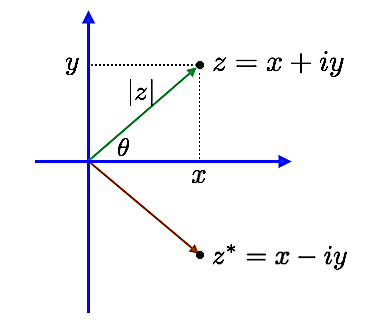
\includegraphics[width=2.4in]{VOLUMEN_1/01_Vectores_Cartesianos/Figuras/Figura1_10}
\caption{ Representaci�n del plano complejo. El eje horizontal recibe el nombre de eje real, y el eje vertical el nombre de eje imaginario.}
\end{minipage}
\end{figure}
%%%%%%%%%%%%%%%%%

Esta representaci�n de n�meros complejos como vectores en el plano (complejo) se conoce con el nombre de Diagrama de Argand\footnote{Jean Robert Argand (Ginebra, Suiza, 18 Julio 1768; Par�s, Francia 13 agosto 1822). Contador pero matem�tico aficionado, propuso esta interpretaci�n de n�meros complejos como vectors en un plano complejo en un libro autoeditado con sus reflexiones que se perdi� y fue rescatado 7 a�os despu�s, fecha a partir de la cual Argand
comenz� a publicar en Matem�ticas.} a pesar que no fue Jean
Argand, sino Caspar Wessel\footnote{Caspar Wessel (Vestby, Noruega 8 junio 1745; 25 marzo 1818, Copenhagen,Dinamarca) Matem�tico noruego que se dedic� principalmente al levantamiento topogr�fico de Noruega. Su trabajo sobre la interpretaci�n de n�meros complejos permaneci� desconocido por casi 100 a�os.} el primero en proponerlo. Por cierto, esta interpretaci�n fue tres veces redescubierta, primero por Caspar Wessel en 1799, luego por Jean Argand en 1806 y finalmente por Gauss\footnote{Johann Carl Friedrich  Gauss (30 abril 1777, Brunswick, Alemania; 23 febrero 1855, G�ttingen, Alemania). Uno de los matem�ticos m�s geniales y precoces de la Historia. Desde los 7 a�os comenz� a mostrar sus condiciones de genialidad. Sus contribuciones en Astronom�a y Matem�ticas son m�ltiples y diversas.} en 1831.

De esta manera, como un recordatorio al plano real podemos ver que:
\[
z=x+iy\quad\leftrightharpoons\quad z=r\left( \cos(\theta)+i\operatorname{sen}(\theta)\right)\,, \quad\text{con: }\left\{
\begin{array}{l}
r=\sqrt{zz^{\ast}}=\left| z\right| =\sqrt{x^{2}+y^{2}} \\
\\
\tan(\theta)=\dfrac{y}{x}\quad\text{donde }-\pi\leq\theta\leq\pi
\end{array}
\right.
\]

Con esta interpretaci�n tendremos:
\begin{center}
\begin{tabular}{lll}
$x={Re}\ z$ & $\rightleftharpoons$ & componente real del vector $z$ o
parte real de $z$ \\
$y={Im} \ z$ & $\rightleftharpoons$ & componente imaginaria del vector $z$
o parte imaginaria de $z$ \\
$r=\sqrt{zz^{\ast}}=\left| z\right| $ & $\rightleftharpoons$ & m�dulo,
magnitud o valor absoluto de $z$ \\
$\theta$ & $\rightleftharpoons$ & �ngulo polar o de fase del n�mero
complejo $z$
\end{tabular}
\end{center}

La interpretaci�n vectorial de n�meros complejos permite que la suma de n�meros complejos: $z_1=x_1 + iy_1$ y $z_2 = x_2 + i y_2$ sea representada por la ``regla del paralelogramo'', es decir, en la representaci�n gr�fica de la suma es f�cil ver que $z_1$ y $z_2$ limitan un  paralelogramo cuya diagonal es $z_1+z_2$. 

Mientras que los productos escalar y vectorial nos llevan a:
\[
z_{1}\cdot z_{2}= {Re}\left( z_{1}z_{2}^{\ast}\right) = {Re}\left( z_{1}^{\ast}z_{2}\right) \quad\wedge\quad
z_{1}\times z_{2}= {Im}\left( z_{1}^{\ast}z_{2}\right) =-{Im}\left( z_{1}z_{2}^{\ast}\right) \,.
\]

Volviendo nuevamente a la relaci�n $\left| z\right|=\sqrt{zz^{\ast}}$, observemos que:
\begin{itemize}
\item $\left| z_1 z_2\right|=\left| z_1\right| \left| z_2\right|$.

Ya que si $\left| z_1 z_2\right|$, $\left| z_1\right|$ y $\left| z_2\right|$ son cantidades positivas, entonces:
\[
\left| z_1 z_2\right|^2= \left(z_1z_2\right) \left(z_1z_2\right)^*
= z_1 z_2 z_1^* z_2^*= z_1z_1^* z_2 z_2^*=
\left| z_1\right|^2 \left| z_2\right|^2 =\left( \left| z_1\right| \left| z_2\right|\right)^2 \,.
\]

\item $\left| z_1+ z_2\right| \leq  \left| z_1\right|+ \left| z_2\right|$.

Veamos:
\begin{eqnarray*}
\left| z_1+ z_2\right|^2 &=&
\left( z_1+ \ z_2 \right)\left( z_1+ \ z_2 \right)^*=
\left( z_1+ z_2 \right)\left( z_1^*+ \ z_2^* \right)=
z_1z_1^* + z_2 z_2^* + z_1z_2^* + z_1^*z_2 = \\
&=&
\left| z_1\right|^2+\left| z_2\right|^2+2{Re}( z_1z_2^*) \leq 
\left| z_1\right|^2+\left| z_2\right|^2+2\left|{Re}( z_1z_2^*)\right| \\ 
&\leq&
\left| z_1\right|^2+\left| z_2\right|^2+2\left| z_1z_2^*\right| =
\left| z_1\right|^2+\left| z_2\right|^2+2\left| z_1\right| \left| z_2^*\right|=
\left| z_1\right|^2+\left| z_2\right|^2+2\left| z_1\right| \left| z_2\right| \\
&=&
\left(\left| z_1\right|+ \left| z_2\right|\right)^2 \,.
\end{eqnarray*}
Notemos que la igualdad $\left| z_1+ z_2\right|= \left| z_1\right|+ \left| z_2\right|$ se satisface si, y s�lo si,  ${Re}(z_1z_2^*)=\left| z_1z_2^*\right|$.

\end{itemize}

\paragraph{Producto escalar:}
El producto escalar definido con anterioridad para vectores puede ser redefinido al caso de vectores con componentes complejas.

Dados los vectores: ${\bf a}=a^i {\bf e}_i$ y ${\bf b}=b^i {\bf e}_i$, con $\{a^i\}$ y  $\{b^i\}$ $\in \mathds{C}$, entonces 
\[
{\bf a} \cdot {\bf b}= \left(a^i\right)^* b_i  \,.
\]
Notemos que con esta definici�n, el producto ${\bf a} \cdot {\bf a}= \left(a^i\right)^* a_i$ siempre ser� un n�mero real. Por lo tanto, $|{\bf a}|=\sqrt{{\bf a} \cdot {\bf a}}$ $\in \mathds{R}$.

Esta definici�n hace que ahora cambien algunas de las propiedades del producto escalar.

\begin{itemize}
\item ${\bf a} \cdot {\bf b}=\left({\bf b} \cdot {\bf a}\right)^*$.
\item $\left(\lambda {\bf a}\right) \cdot {\bf b}= 
\lambda^* \ {\bf a} \cdot {\bf b}$.
\item $ {\bf a} \cdot (\lambda{\bf b})= 
\lambda \ {\bf a} \cdot {\bf b}$.
\end{itemize}



\subsection{F�rmulas de Euler y De Moivre}
\label{FormulaEulerMoivre}
\index{F�rmulas de Euler}
\index{Euler!F�rmulas de }
\index{F�rmulas de De Moivre}
\index{De Moivre!F�rmulas de}
\index{Taylor!Brook Taylor}
\index{N�meros complejos!F�rmulas de Euler y De Moivre}
En cursos anteriores, nos hemos tropezado con la expansi�n en Taylor\footnote{Brook Taylor (18 agosto 1685, Edmonton, Inglaterra; 29 diciembre 1731, Londres, Inglaterra) F�sico y Matem�tico ingl�s contempor�neo de Newton y Leibniz y junto con ellos particip� profundamente en el desarrollo del c�lculo diferencial e integral. Adem�s de sus aportes al estudio del magnetismo,
capilaridad y termometr�a, desarroll� el �rea de diferencias finitas que hasta hoy utilizamos para c�lculos en computaci�n. Invent� la integraci�n por partes y descubri� la serie que lleva su nombre.} de funciones, �sta serie permite expresar cualquier funci�n anal�tica\footnote{B�sicamente, una funci�n anal�tica es una funci�n que puede expresarse como una serie de potencias convergente.} alrededor de un punto $x_{0}$ como una serie infinita de potencias del argumento de la funci�n, esto es:
\[
f\left( x\right) =f(x_{0})+\left. \frac{\mathrm{d }f\left( x\right) }{\mathrm{d
}x}\right| _{x=x_{0}}\left( x-x_{0}\right) +\frac{1}{2}\left. \frac{\mathrm{d
}^{2}\mathrm{ }f\left( x\right) }{\mathrm{d }x^{2}}\right|
_{x=x_{0}}\left( x-x_{0}\right) ^{2}+\frac{1}{3!}\left. \frac{\mathrm{d}^{3}
\mathrm{ }f\left( x\right) }{\mathrm{d }x^{3}}\right| _{x=x_{0}}\left(
x-x_{0}\right) ^{3}+\cdots \cdots
\]
O de manera equivalente:
\[
f\left( x\right)  =C_{n}\left( x-x_{0}\right) ^{n}\qquad \text{con }\,\, 
C_{n}=\frac{1}{n!}\left. \frac{\mathrm{d}^{n}\mathrm{\ }f\left( x\right) }{\mathrm{d\ }x^{n}}\right| _{x=x_{0}} \quad \text{y }\,\,  n=0,1,2,3, \dots
\]

Si consideramos que $x_{0}=0$, podremos ver a continuaci�n algunos desarrollos en series de funciones elementales:
\begin{eqnarray*}
e^{x}&=&1+x+\frac{1}{2}x^{2}+\frac{1}{6}x^{3}+\frac{1}{24}x^{4}+\frac{1}{120} x^{5}+\frac{1}{720}x^{6}+\frac{1}{5040}\allowbreak x^{7}+\cdots \cdots  \\
\cos(x)& =& 1-\frac{1}{2}x^{2}+\frac{1}{24}x^{4}-\frac{1}{720}x^{6}+\cdots \cdots  \\
\operatorname{sen}(x)& =&x-\frac{1}{6}x^{3}+\frac{1}{120}x^{5}-\frac{1}{5040}x^{7}+\cdots \cdots
\end{eqnarray*}

Es f�cil convencerse que para la serie de $e^{x}$ se tiene:
\[
e^{i\theta }=1+i\theta -\frac{1}{2}\theta ^{2}+\left( -\frac{1}{6}i\right)
\theta ^{3}+\frac{1}{24}\theta ^{4}+\frac{1}{120}i\theta ^{5}-\frac{1}{720}
\theta ^{6}+\left( -\frac{1}{5040}i\right) \theta ^{7}+\cdots \cdots
\]
y que puede arreglarse como: 
\[
e^{i\theta} =\underset{\cos(\theta) }{\underbrace{\left( 1-\frac{1}{2}
\theta ^{2}+\frac{1}{24}\theta ^{4}-\frac{1}{720}\theta ^{6}+\cdots \cdots
\right) }}+i\underset{\operatorname{sen}(\theta) }{\underbrace{\left( \theta -\frac{1}{6}\theta ^{3}+\frac{1}{120}\theta ^{5}-\frac{1}{5040}\theta ^{7} +\cdots \cdots \right)}}
\]
obteni�ndose  la importante relaci�n: 
\[
e^{i\theta} =\cos(\theta) +i\operatorname{sen}( \theta)\,,
\]
conocida como la relaci�n de Euler\footnote{Leonhard Euler (15 abril 1707, Basilea, Suiza; 18 septiembre 1783, San Petersburgo, Rusia). Uno de los matem�ticos m�s prol�ficos de todos los tiempos. Desarroll� inmensamente campos como la geometr�a anal�tica y trigonometr�a, siendo el primero que consider� el coseno y el seno como funciones. Hizo aportes significativos en el desarrollo del c�lculo diferencial e integral as� como tambi�n, astronom�a, elasticidad y mec�nica de medios continuos.}. La f�rmula de Euler, para  $-\pi < \theta < \pi$ resulta en los siguientes simp�ticos resultados:
\[
i=e^{i\frac{\pi}{2}}\,,\quad -1=e^{i\pi}\,,\quad -i=e^{-i\frac{\pi}{2}} \,,\quad 1=e^{i2k\pi} \quad \, \mbox{con  }  k=0, \pm 1,\pm 2 , \pm 3 \dots
\] 

Entonces, tenemos tres formas de representar un n�mero complejo:
\[
z=x+iy\quad \leftrightharpoons \quad z=|z|\left( \cos(\theta) +i\operatorname{sen} (\theta)\right) \quad \leftrightharpoons \quad
z=|z| e^{i\theta } \,.
\]

La expresi�n $z=x+iy$ se conoce como forma cartesiana de representaci�n de un n�mero complejo, la forma $z=r\left(\cos(\theta) +i\operatorname{sen}(\theta) \right) $ ser� la forma trigonom�trica o polar y la expresi�n $z=r e^{i\theta}$ ser� la forma de Euler.  

Es importante notar una sutileza impl�cita en esta notaci�n. La forma cartesiana representa un�vocamente a un n�mero complejo, mientras que la forma polar (y la de Euler), es ambigua, ya que:
\[
z=r\left(
\cos(\theta) +i\mbox{sen}(\theta) \right)= r\left(\cos(\theta +2n\pi)
+i\mbox{sen}(\theta +2n\pi)\right)\,, \quad n=0,\pm1, \pm 2, \pm 3, \dots 
\]
Es decir, existen varios valores del argumento que definen el mismo n�mero complejo. Por ejemplo, el n�mero $z=1+\sqrt{3} i$ lo podemos representar de las siguientes maneras:
\begin{eqnarray*}
z =1+\sqrt{3} i &=& 2e^{\frac{\pi}{3}i}= 2\left[ \cos\left(\frac{\pi}{3}\right)+i\mbox{sen}\left(\frac{\pi}{3}\right)\right] \\
&=&  2e^{\left(\frac{\pi}{3}+2n\pi\right)i}= 2\left[ \cos\left(\frac{\pi}{3}+2n\pi\right)+i\mbox{sen}\left(\frac{\pi}{3}+2n\pi\right)\right]\,.
\end{eqnarray*}

Analicemos estas situaciones con m�s detalle. Primero es importante notar que $r$ es siempre positivo, mientas que el �ngulo $\theta$ puede tomar infinitos valores incluyendo valores negativos. Como ya vimos, $\theta$ se relaciona con las coordenadas cartesianas por la ecuaci�n $\tan(\theta)=y/x$, y donde es necesario especificar el cuadrante para su c�lculo. A cada valor del �ngulo se le denomina el {\it argumento de} $z$. 

Por lo tanto, si tenemos un n�mero complejo $z$ denotaremos por $\mbox{arg}(z)$ a:
\[
\mbox{arg}(z)=\{ \theta \in \mathds{R} \,\, /  \,\,  |z| (\cos(\theta) +i\mbox{sen}(\theta) ) \}\,.
\]
Esto significa que dos n�meros complejos $z_1$ y $z_2$ ser�n iguales si: $|z_1|=|z_2|$ y $\mbox{arg}(z_1)=\mbox{arg}(z_2)$.

Dado un n�mero complejo, $z \neq 0$, existe un �nico argumento $\Theta$ que se encuentra en el intervalo $[-\pi, \pi]$, y  lo representaremos por $\mbox{Arg}(z)$, el {\it argumento principal} o {\it valor principal}, de manera que:
\[
\mbox{arg}(z)=\mbox{Arg}(z)+2n\pi \,,  \qquad n=0,\pm1, \pm 2, \pm 3, \dots 
\]

Un n�mero complejo, digamos $z=-1-i$ (tercer cuadrante) tendr� como valor principal: 
\[
\tan(\Theta)=\frac{y}{x}= 1 \,\, \Rightarrow \,\, 
\mbox{Arg}(-1-i)=-\frac{3\pi}{4}\,.
\]
Nota: no debe tomarse el valor $-\frac{5\pi}{4}$, ya que $-\pi \leq\Theta\leq \pi$. 

Lo que si es cierto es que:
\[
\mbox{arg}(-1-i)=-\frac{3\pi}{4}+2n\pi \,, \qquad n=0,\pm1, \pm 2, \pm 3, \dots
\]
%%%%%%%%%%%%%%%%%
\begin{figure}[h]
\begin{minipage}{7.4cm}
Otro aspecto a rescatar de la forma de Euler o exponencial, es que la ecuaci�n: 
\[
z= r e^{i \theta} \,,\qquad 0\leq \theta \leq 2\pi \,,
\]
no es m�s que una representaci�n param�trica del c�rculo $|z|=r$, es decir, de un c�rculo de radio $r$ y centrado en el origen. 

Por lo tanto, un c�rculo centrado en $z_0$ y de radio $R$ tendr� como ecuaci�n param�trica:
\[
|z-z_0|=R \,\, \Rightarrow \,\  z= z_0 +R e^{i \theta} \,,
\]
con  $ 0\leq \theta \leq 2\pi$. Como podemos apreciar en la figura \ref{circuloparametrico}.

\end{minipage} \hfill 
\begin{minipage}{8.0cm} 
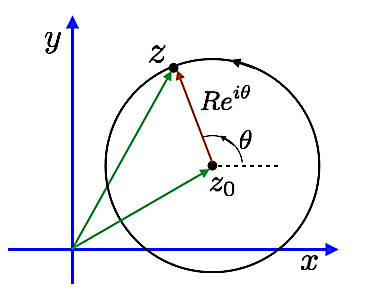
\includegraphics[width=2.3in]{VOLUMEN_1/01_Vectores_Cartesianos/Figuras/Figura1_11}
\caption{Representaci�n en el plano complejo del c�rculo $|z-z_0|=R$.}
\label{circuloparametrico}
\end{minipage}
\end{figure}
%%%%%%%%%%%%%%%%%

Es claro que las sumas de n�meros complejos se plantean m�s f�cilmente en su forma cartesiana. Mientras las multiplicaci�n y divisi�n ser�n directas en la forma de Euler. Si $z_{1}=|z_{1}| e^{i\theta _{1}}$ y $z_{2}=|z_{2}| e^{i\theta _{2}}$, entonces: 
\begin{equation}
z_{1}z_{2}=|z_{1}| e^{i\theta_{1}} |z_{2}|  e^{i\theta_{2}}=
|z_{1}| |z_{2}| e^{i\left(\theta_{1}+\theta_{2}\right)}=|z_{1}z_{2}|\left( \cos \left( \theta_{1}+\theta_{2}\right) +i\mbox{sen} \left( \theta_{1}+\theta_{2}\right) \right) \,.
\label{z1porz2}
\end{equation}

Esto significa que para multiplicar dos n�meros complejos se debe, por un lado, multiplicar sus m�dulos y por el otro, sumar sus argumentos. Geom�tricamente, al sumarse los argumentos, la multiplicaci�n es en realidad un giro en el plano complejo por el producto de sus m�dulos, es decir, si multiplicamos un n�mero por $i$, el resultado es un giro de un cuarto de vuelta hacia la izquierda, es por eso, que $i^2=-1=e^{i \pi}$.

Mientras que para la divisi�n: 
\[
\frac{z_{1}}{z_{2}}=
\frac{|z_{1}|e^{i\theta_{1}}}{|z_{2}| e^{i\theta_{2}}}=
\frac{|z_{1}| }{|z_{2}| }e^{i\left(\theta_{1}-\theta_{2}\right)}=
\frac{|z_{1}| }{|z_{2}| }\left( \cos \left( \theta_{1}-\theta_{2}\right) +i\mbox{sen} \left( \theta_{1}-\theta_{2}\right) \right) \,.
\]

Podemos notar de esta �ltima expresi�n que el inverso de un n�mero complejo diferente se cero es:
\begin{equation}
z^{-1}=\frac{1}{z}=\frac{1}{|z| }e^{-i\theta} \,.
\label{invz}
\end{equation}	

Se puede mostrar que a partir de (\ref{z1porz2}) y de  (\ref{invz}) resulta que:
\begin{eqnarray*}
\mbox{arg}(z_1z_2)&=&\mbox{arg}(z_1)+\mbox{arg}(z_2) \,, \\
\mbox{arg}\left(\frac{z_1}{z_2} \right)&=
&\mbox{arg}(z_1)-\mbox{arg}(z_2) \,.
\end{eqnarray*}


Por otro lado, notemos lo siguiente. Si $z=x+iy$, entonces: 
\[
e^{z}=e^{\left(x+iy\right)}=e^{x}e^{i y}=e^{x}\left( \cos(y)+i\mbox{sen}(y)\right)\,,
\]
y a partir de la relaci�n o f�rmula de Euler se puede demostrar:
\[
z^n=|z|^n \left(e^{i\theta }\right) ^{n}=|z|^n e^{in\theta }
\,\, \Rightarrow \,\,  
|z|^n\left( \cos( \theta) +i\mbox{sen} (\theta)\right) ^{n}=
|z|^n\left( \cos \left( n\theta \right) +i\mbox{sen} \left(n\theta \right)\right)\,,
\]
con $n$ entero.  

De manera que llegamos a la f�rmula de  De Moivre:\footnote{Abraham De Moivre  (26 mayo 1667 en Vitry-le-Fran\c{c}ois, Francia; 27 noviembre 1754, Londres, Inglaterra) Matem�tico franc�s que tuvo que emigrar a Inglaterra por razones religiosas. Contempor�neo de Newton, Leibniz y Halley, fue pionero con sus contribuciones en geometr�a anal�tica y teor�a de probabilidades.}
\[
\left( \cos( \theta) +i\mbox{sen} (\theta)\right) ^{n}=
\cos \left( n\theta \right) +i\mbox{sen} \left(n\theta \right) \,, \quad \text{con }n\text{ entero}.
\]


\subsection{Algunas aplicaciones inmediatas}
\index{N�meros complejos!Aplicaciones f�rmulas de Euler y De Moivre} Presentaremos algunas aplicaciones inmediatas la f�rmula de De Moivre en diferentes  �mbitos. 

\subsubsection{Identidades trigonom�tricas}
\index{F�rmulas de De Moivre!Identidades trigonom�tricas}

La primera de las aplicaciones de la f�rmula de De Moivre es
para construir identidades trigonom�tricas en las cuales se expresa el coseno, o el seno, de factores de un �ngulo. Veamos las siguientes (nada triviales) identidades trigonom�tricas:
\[
\cos(3\theta)=4\cos^{3}(\theta)-3\cos(\theta)\qquad\text{o}\qquad\operatorname*{sen}
(3\theta)=3\operatorname*{sen}(\theta)-4\mbox{sen}^{3}(\theta)\,.
\]

Para demostrar estas (y otras) identidades utilizamos la
f�rmula de De Moivre, es decir:
\begin{align*}
\cos(3\theta)+i\operatorname*{sen(}3\theta) &  =\left(
\cos(\theta)+i\operatorname{sen}(\theta)\right)^{3}\\
&  =\cos^{3}(\theta)-3\cos(\theta)\operatorname{sen}^{2}(\theta)+i\left(
3\cos^{2}(\theta) \operatorname{sen}(\theta)-\operatorname{sen}^{3}(\theta)\right) \,.
\end{align*}

Igualando ahora parte real e imaginaria tendremos:
\begin{eqnarray*}
\cos(3\theta)&=&\cos^{3}(\theta)-3\cos(\theta)\operatorname{sen}^{2}(\theta)=\cos^{3}(\theta)-3\cos(\theta)\left(  1-\cos^{2}(\theta)\right)
=4\cos^{3}(\theta)-3\cos(\theta)\,, \\ 
\mbox{sen}(3\theta) &=&3\cos^{2}(\theta)\mbox{sen}(\theta)-\mbox{sen}^{3}(\theta) =3\left(  1-\mbox{sen}^{2}(\theta)\right)  \mbox{sen}(\theta)-\mbox{sen}^{3}(\theta)=3\mbox{sen}(\theta)-4\mbox{sen}^{3}(\theta)\,.
\end{eqnarray*}

El m�todo puede extenderse a expresiones de senos y cosenos de $n\theta$.

Igualmente podemos desarrollar un m�todo para encontrar expresiones de potencias de funciones trigonom�tricas en t�rmino de funciones de factores de �ngulo del tipo $\left(  \cos(\theta)\right)  ^{n}=F\left( \cos(n\theta),\operatorname*{sen}(n\theta)\right)$.  Para empezar, supongamos que tenemos un n�mero complejo de m�dulo $1$, de tal forma que:
\[
z=e^{i\theta}=\cos(\theta)+i\operatorname{sen}(\theta) \,\, \Rightarrow \,\,  \left\{
\begin{array}
[c]{l}
z^{n}+\dfrac{1}{z^{n}}=2\cos (n\theta)\\
\\
z^{n}-\dfrac{1}{z^{n}}=2i\operatorname*{sen}(n\theta)
\end{array}
\right.
\]

Estas identidades surgen de manera inmediata a partir de:
\begin{align*}
z^{n}+\frac{1}{z^{n}}  & =\left(  \cos(\theta)+i\operatorname{sen}(\theta)\right)
^{n}+\left( \cos(\theta)+i\operatorname{sen}(\theta)\right)  ^{-n}=\left(  \cos
(n\theta)+i\operatorname{sen} (n\theta) \right)  +\left(  \cos\left(
-n\theta\right)  +i\operatorname{sen}\left(  -n\theta\right)
\right)  \\
& =\cos (n\theta)+i\operatorname{sen} (n\theta)+\cos (n\theta)-i\operatorname{sen} (n\theta) =2\cos (n\theta) \,,
\end{align*}
igualmente puede demostrarse la segunda de las afirmaciones
anteriores. 

Supongamos adem�s que $n=1,$ con lo cual se cumple que:
\[
z+\dfrac{1}{z}=e^{i\theta}+e^{-i\theta}=2\cos(\theta)\qquad\text{y}\qquad
z-\dfrac{1}{z}=e^{i\theta}-e^{-i\theta}=2i\operatorname{sen}(\theta)\,,
\]
que tambi�n lo sab�amos desde la m�s temprana edad de nuestros cursos de bachillerato. 

Ahora bien, lo que quiz� no sab�amos en ese entonces (y quiz� ahora tampoco) es que a partir de aqu� podemos construir, expresiones como:
\[
\cos(\theta)=\frac12 \left(z+\dfrac{1}{z}\right) \,\, \Rightarrow \,\, 
\cos^{5}(\theta)=\frac{1}{2^{5}}\left(  z+\dfrac{1}{z}\right)^{5}=
\frac{1}{2^{5}}\left[  \left(  z^{5}+\frac{1}{z^{5}}\right)  +\left(5z^{3}
+\frac{5}{z^{3}}\right)  +\left(  10z+\frac{10}{z}\right)  \right]\,,
\]
es decir:
\[
\cos^{5}(\theta)=\frac{1}{2^{5}}\left[
2\cos(5\theta)+10\cos(3\theta)+20\cos( \theta)\right]\,.
\]

De la misma manera se puede proceder con otras potencias y con potencias de la funci�n seno.

\subsubsection{Ra�ces de polinomios}
\index{F�rmulas de De Moivre!Ra�ces de polinomios}

Las ra�ces de un n�mero complejo se obtienen de la relaci�n:
\[
z^{1/n}= \left[|z| \left(\cos\left( \theta \right)+i\ \mbox{sen}\left(\theta \right) \right) \right]^{1/n}= |z|^{1/n} \left[\cos\left( \frac{\theta+2k\pi}{n} \right)+i\ \mbox{sen}\left(\frac{\theta+2k\pi}{n} \right) \right] \,,
\]
donde $k=0,1, \dots n-1$. De manera que la f�rmula de De Moivre nos puede ayudar para encontrar ra�ces de polinomios. 

Supongamos, para empezar, que queremos encontrar las $n$ ra�ces de la ecuaci�n:
\[
z^{n}=1 \,.
\]  

Para ello procedemos con el siguiente artificio:
\[
z^{n}=1=e^{i\left( 2\pi k \right)} =
\cos\left( 2\pi k \right) +i\mbox{sen}\left( 2\pi k \right) \,, 
\quad \text{donde  } k=0,1,2,....
\]
con lo cual las $n$ ra�ces de la ecuaci�n $z^{n}=1$ ser�n:
\begin{equation}
z^{n}=1= e^{i\left( 2\pi k \right)} \,\,  \Rightarrow \,\,  
z=e^{i\left(\frac{2\pi k}{n}\right)}\,,
\label{zetaalan}
\end{equation}
esto es:
\[
z_{0}=1;\quad z_{1}=e^{2\pi i\left(  \frac{1}{n}\right)};
\quad z_{2}=e^{2\pi i\left(  \frac{2}{n}\right)  };
\quad z_{3}=e^{2\pi i\left(\frac{3}{n}\right)  };\cdots
\quad z_{n-2}=e^{2\pi i\left(  \frac{n-2}{n}\right)  };
\quad z_{n-1}=e^{2\pi i\left(  \frac{n-1}{n}\right)  } \,,
\]
es decir, $n$ ra�ces corresponder�n a los $n$ valores de
$k=0,1,2,\cdots n-2,n-1$. Mayores valores de $k$ no proveen nuevas ra�ces.

Las ra�ces de la ecuaci�n $z^{3}=1$ ser�n entonces: 
\[
z=e^{i\left(  \frac{2\pi k}{3}\right)} \,\,  \Rightarrow \,\,  
z_0=1\,, \,\,  z_1=e^{i\left(  \frac{2\pi }{3}\right)} \,, \,\, 
z_2= e^{i\left(  \frac{4\pi}{3}\right)}\,. 
\]

Como veremos m�s adelante, estas propiedades pueden extenderse a ra�ces de polinomios que contengan m�s t�rminos. 

Una afirmaci�n que nos han dicho, y que quiz� no sepamos de d�nde viene, es que \textit{si un polinomio con coeficientes reales tiene ra�ces complejas, ellas ser�n complejas conjugadas unas de otras}. Vale decir, si $z^{5}-z^{4}+2z-2=0$ tiene como ra�z $ \left( 1+i \right)$, tambi�n tendr� como ra�z $ \left(1 -i \right)$.

Esta afirmaci�n se prueba de forma general si suponemos que tenemos la siguiente ecuaci�n:
\[
a_{k}\ z^{k}=0\,,\quad\text{con }k=0,1,2,\cdots n-1,n \,\, \Rightarrow \,\,   
a_{0}+a_{1}\ z+a_{2}\ z^{2}\cdots+a_{n-1}\ z^{n-1}+a_{n}\ z^{n}=0\,,
\]
donde los coeficientes $a_{0}, a_1, a_{2},\cdots,a_{n-1}, a_{n}$ los
suponemos reales, esto es: $a_{k}=a_{k}^{\ast}$ para todos los
valores del �ndice $k$. 

Al tomar el complejo conjugado nos queda:
\[
a_{0}^{\ast}+a_{1}^{\ast}\ z^{\ast}+a_{2}^{\ast }\left(  z^{\ast}\right)
^{2}\cdots+a_{n-1}^{\ast}\left(  z^{\ast}\right)^{n-1}+a_{n}^{\ast}\left(z^{\ast}\right)^{n}=0 \,,
\]
y como los coeficientes son reales tenemos que:
\[
a_{0}+a_{1} z^{\ast}+a_{2}\left(  z^{\ast}\right) ^{2}\cdots+a_{n-1}\left(
z^{\ast}\right)  ^{n-1}+a_{n}\left(  z^{\ast }\right)  ^{n}=0\,,
\]
esto nos dice que si $z$ es soluci�n tambi�n lo ser� $z^{\ast}$ ya que la ecuaci�n es la misma por tener los mismos coeficientes (reales).


\subsubsection{Logaritmos y potencias de n�meros complejos}
\index{F�rmulas de De Moivre!Logaritmos y potencias de n�meros complejos}

La motivaci�n surge cuando queremos resolver la ecuaci�n:
\begin{equation}
e^{w}=z=re^{i\Theta} \,,\quad \mbox{con}\quad w,z \in \mathds{C} \quad \mbox{y}\quad   -\pi <\Theta <\pi\,.
\label{expw}
\end{equation}

Notemos que al despejar $w$ en realidad lo que tenemos es la funci�n logar�tmica, que como veremos en su debido tiempo puede escribirse de la forma $w=u+iv$. Por lo tanto:
\[
e^{u+iv}=e^{u}e^{iv}=re^{i\Theta} \,\, \Rightarrow \,\, 
e^{u}=r \,\, \wedge \,\, v=\Theta +2\pi n \,.
\]
donde $n$ es un entero. Por lo tanto, es claro que: 
\[
e^{u}=r \,\, \Rightarrow \,\, u=\ln(r)\,,
\]
y que la ecuaci�n (\ref{expw}) se satisface si y s�lo si:
\[
w=\ln(r)+i\left(\Theta +2\pi n\right) \,,\quad \mbox{con}\quad 
n=0,\pm1, \pm2,\pm3, \dots 
\]
Por lo tanto, si definimos la funci�n multivaluada: 
\begin{equation}
\mbox{Log}(z)\equiv \ln|r|+i\left(\Theta +2\pi n\right) \,,\quad 
\mbox{con}\quad  n=0,\pm1, \pm2,\pm3, \dots 
\label{logz}
\end{equation}
podemos escribir la relaci�n:
\[
e^{\mbox{Log}(z)}=z \quad  \mbox{con}\quad z\neq0 \,.
\]

Llamaremos {\it valor principal} de $\mbox{Log}(z)$ al valor que se obtiene cuando $n=0$ en la ecuaci�n (\ref{logz}) y lo denotaremos con $\mbox{Ln}(z)$.
\begin{equation}
\mbox{Ln}(z)= \ln|r|+i\Theta \,.
\label{Lnz}
\end{equation}

Notemos que �sta es una funci�n univaluada cuando $z\neq0$, y adem�s, si combinamos (\ref{logz}) y (\ref{Lnz}) obtenemos:
\[
\mbox{Log}(z)=\mbox{Ln}(z)+i\ 2\pi n \,,\quad 
\mbox{con}\quad  n=0,\pm1, \pm2,\pm3, \dots 
\]

Podemos ver que cuando $z$ es un n�mero real positivo, es decir, $z=re^{i 0}$, entonces recobramos la funci�n logar�tmica usual:
\[
\mbox{Ln}(z)=\mbox{Ln}(r)= \ln(r) \,.
\]

En consecuencia, podemos ver que: 
\begin{eqnarray*}
\mbox{Log}(1)&=&\ln(1)+i\left(0 +2\pi n\right) \quad 
 \,\, \wedge \,\, \quad\mbox{Ln}(1)=0 \\
\mbox{Log}(-1)&=&\ln(1)+i\left(\pi +2\pi n\right)\quad 
  \,\, \wedge \,\, \quad \mbox{Ln}(-1)=i \pi 
\end{eqnarray*}
con $n=0,\pm1, \pm2,\pm3, \dots$

Por otro lado, podemos ver tambi�n: 
\begin{eqnarray*}
\ln(z^n)&=&\ln\left[\left\{|z|\left(\cos(\theta) + i \ \mbox{sen}(\theta) \right) \right\}^n\right]=n \ln\left[|z|\left(\cos(\theta) + i \ \mbox{sen}(\theta) \right) \right]= n \ln\left[|z| \ e^{i \theta}  \right] \\ 
&=& n \ln\left(|z|\right) + n (\theta+2k\pi)i = 
n \ln\left(|z|\right) + (n \theta) i + (2nk \pi) i \,, \quad \mbox{con }  k \,\, 
\mbox{entero}\,.
\end{eqnarray*}



\subsection{{\color{Fuchsia}Ejemplos}}

\begin{enumerate}

\item En la secci�n \ref{FormulaEulerMoivre}, vimos que para el n�mero complejo $z=-1-i$, resultaba que:
\[
\mbox{arg}(-1-i)=-\frac{3\pi}{4}+2n\pi \qquad n=0,\pm1, \pm 2, \pm 3, \dots
\]

Si lo queremos escribir en la forma exponencial tenemos que hacer lo siguiente:
\[
|z|=\sqrt{(-1)^2+(-1)^2}= \sqrt{2}\,\, \Rightarrow \,\,
-1-i= \sqrt{2}e^{-i\left(\frac{3\pi}{4}\right)}\,.
\]
Pero en realidad hay infinitas posibilidades para la forma exponencial de $z=-1-i$:
\[
-1-i= \sqrt{2}e^{i\left(-\frac{3\pi}{4}+2n\pi\right)} \,,\qquad n=0,\pm1, \pm2, \dots
\]

\item Consideremos el n�mero $z=2+2 i$, para representarlo en la forma polar debemos calcular primeramente su m�dulo:
\[
|z|=\sqrt{x^2+y^2}=\sqrt{2^2+2^2}=\sqrt{8}=2\sqrt{2}\,.
\]
y luego el argumento:
\[
\tan(\theta)=\frac{y}{x}=\frac{2}{2} \,\, \Rightarrow \,\, \theta=\arctan(1)= \frac{\pi}{4}\,. 
\]

Por lo tanto, $z=2+2 i=2\sqrt{2}\left(\cos(\pi/4)+i\ \mbox{sen}(\pi/4) \right)$, es un punto ubicado en el primer cuadrante cuyo radio vector hace un �ngulo de $45^{\circ}$ con respecto al eje $x$. 

En cambio, para el n�mero complejo $z=-\sqrt{3}+i$, resulta:
\[
|z|=\sqrt{(-\sqrt{3})^2+1^2}=\sqrt{4}=2\,, \quad 
\theta=\arctan\left(-\frac{1}{\sqrt{3}}\right)= -\frac{\pi}{6}\,.
\]
Aqu� debemos tener cuidado, pues el argumento principal en realidad es:
\[
\theta= \pi-\frac{\pi}{6}=\frac{5\pi}{6}\,.
\]
 $z=-\sqrt{3}+i=2\left(\cos(5\pi/6)+i\ \mbox{sen}(5\pi/6) \right)$, es un punto ubicado en el segundo cuadrante cuyo radio vector hace un �ngulo de $150^{\circ}$ con respecto al eje $x$.

\item Supongamos la siguiente ecuaci�n polin�mica con sus ra�ces:
\[
z^{5}-z^{4}+2z-2=0 \,\, \Rightarrow \,\,
\left( z^{4}+2\right)  \left(
z-1\right) =0 \,\, \Rightarrow \,\, \left\{
\begin{array}
[c]{l}
z^{4}+2=0\,\, \Rightarrow \,\,  z^{4}=-2\\
\\
z-1=0 \,\, \Rightarrow \,\, z=1
\end{array}
\right.
\]
Entonces, de la ecuaci�n (\ref{zetaalan}) podemos ver que:
\begin{align*}
z^{4}  & =-2(1)=-2\left(e^{i\left( 2\pi k \right)  }\right)
\,\, \Rightarrow \,\, 
z= \left[ -2\left(e^{i\left( 2\pi k \right)  }\right) \right]^{1/4}
= (-2)^{1/4}e^{i\left(  \frac{2\pi k}{4}\right)}
= \frac{{2}^{3/4}}{2} \left( 1+i \right)  e^{i\left(  \frac{2\pi k}{4}\right) } \,,
\end{align*}
donde hemos utilizado el hecho de que: $(-1)^{1/4}=i^{1/2}= \left(e^{i\frac{\pi}{2}}\right)^{1/2}= e^{i\frac{\pi}{4}}=
\frac{\sqrt{2}}{2}(1+i)$\,.

Por lo tanto:
\begin{eqnarray*}
z_0&=&\frac{1}{{2}^{1/4}} \left( 1+i \right)  \,, 
\qquad\qquad\qquad\qquad\qquad\quad 
z_1=\frac{1}{{2}^{1/4}} \left( 1+i \right) e^{i\left(  \frac{\pi}{2}\right) } =
\frac{i}{{2}^{1/4}}\left( 1+i \right)  \\
z_2&=&\frac{1}{{2}^{1/4}} \left( 1+i \right) e^{i\left( {\pi}\right) } =
-\frac{1}{{2}^{1/4}} \left( 1+i \right) \,, \quad
z_3=\frac{1}{{2}^{1/4}} \left( 1+i \right)e^{i\left(  \frac{3\pi }{2}\right) } =
-\frac{i}{{2}^{1/4}} \left( 1+i \right)\,.
\end{eqnarray*}

Entonces, la ecuaci�n $z^{5}-z^{4}+2z-2=0$, tendr� las siguientes cinco ra�ces:
\[
z_0=\frac{1}{{2}^{1/4}} \left( 1+i \right) \,, \quad 
z_1=-\frac{1}{{2}^{1/4}}\left(1- i \right) \,, \quad 
z_2=-\frac{1}{{2}^{1/4}} \left( 1+i \right) \,, \quad 
z_3=\frac{1}{{2}^{1/4}} \left(1 -i \right)\,, \quad 
z_4=1\,.
\]

\item
Ahora consideremos el siguiente polinomio complejo: 
\[
P(z)=z^{6} -z^{5} +4z^{4} -6z^{3} +2z^{2} -8z +8 = 0\,.
\]
Si por alg�n m�todo comprobamos que $(z^{3} -2)$ es uno de sus factores, entonces podremos encontrar las ra�ces del polinomio $P(z)$.  

Veamos,  claramente si $(z^{3} -2)$ es un factor, entonces  podemos expresar:
\[
P(z)=z^{6} -z^{5} +4z^{4} -6z^{3} +2z^{2} -8z +8 = (z^{3} -2)(z^{3} - z^{2} + 4z - 4)= (z^{3} -2)(z -1)({z}^{2}+4)\,,
\]
con lo cual, como $z$ es complejo, hay que tener cuidado con las ra�ces encubiertas. Entonces, la ra�ces son:
\[
z^{3}=2\,,\quad z=1\,, \quad z^2=-4\,.
\]

\begin{itemize}
\item Para  $z^2=-4\,\, \Rightarrow \,\,  z= \pm 2i$\,.

\item Para  $z^{3}=2 \,\, \Rightarrow \,\,  z^{3} =2\left(e^{i\left( 2\pi k \right) }\right) \,\, \Rightarrow \,\, 
z= \left[ 2\left(e^{i\left( 2\pi k \right)  }\right) \right]^{1/3}
= 2^{1/3}e^{i\left(  \frac{2\pi k}{3}\right)}$.

Por lo tanto:
\[
z_0=2^{1/3} \,, \quad 
z_1=2^{1/3}e^{i\left(  \frac{2\pi }{3}\right)} =
-\frac{2^{1/3}}{2}\left[1-\sqrt{3} i  \right]  \,, \quad 
z_2=2^{1/3}e^{i\left(  \frac{4\pi }{3}\right)} =
-\frac{2^{1/3}}{2}\left[1+\sqrt{3} i  \right]  \,.
\]
\end{itemize}

La ecuaci�n: $z^{6} -z^{5} +4z^{4} -6z^{3} +2z^{2} -8z +8 = 0$, tendr� las siguientes seis ra�ces:
\[
z=\sqrt[3]{2} \,, \quad 
z=-\frac{1}{\sqrt[3]{4}}\left[1\pm \sqrt{3}\ i  \right]  \,, \quad 
z = 1 \,, \quad z = \pm 2i \,.
\]


\item Consideremos:
\[
\mbox{Log}\left(  -3i\right) =\mbox{Log}\left[
3e^{i\left(-\frac{\pi}{2}+2n\pi\right)  }\right]  =\ln(3)+i\left(  -\frac{\pi}{2}
+2n\pi\right)  \quad\text{con }n=0,1,2,\cdots
\]
decimos que el valor principal de $\mbox{Log}\left(-3i\right)$ ser� $\mbox{Ln}=\ln(3)-i\frac{\pi}{2}$\,.

Con la misma intuici�n se procede con las potencias de n�meros complejos. 

Si queremos evaluar $z=i^{-5i}$ tendremos que proceder como sigue:
\[
z=i^{-5i}\,\, \Rightarrow \,\,\mbox{Log}\left( z\right) =\mbox{Log}
\left(  i^{-5i}\right)  =-5i\mbox{Log}\left(i\right)
=-5i\mbox{Log}\left[  e^{i\left(
\frac{\pi}{2}+2n\pi\right)  }\right] = {5\left(\frac{\pi}{2}+2n\pi\right)} \,,
\]
con lo cual $z=i^{-5i}$  �es un n�mero real!

Para finalizar consideremos otro par de casos de potencias y logaritmos: $i^{i}$ y 
$\mbox{Log} \left[ \left\{ \sqrt{3} + i \right\}^{3} \right]$. 
\begin{itemize}
\item 
$
 i^{i} =\left[ e^{i\left( \frac{\pi}{2} +2n \pi \right)} \right]^{i} =  e^{i^{2} \left( \frac{\pi}{2} +2n \pi \right)} =
    e^{-\left( \frac{\pi}{2} +2n \pi \right)}\,.
$
\item 
$
\mbox{Log} \left[ \left( \sqrt{3} + i \right)^{3} \right] = 3 \mbox{Log}\left[ 2 e^{i\left(\arctan\left( \frac{1}{\sqrt{3}} \right)\right)} \right] =
    3 \left[\ln(2) +  i\left(\arctan \left(\frac{1}{\sqrt{3}}\right) +2n\pi \right) \right] = \ln(8) + i\left(\frac{\pi}{2} +6n \pi \right)$.
\end{itemize}

\end{enumerate}

\newpage
\subsection{{\color{red}Practicando con Maxima}} 

{\bf Maxima} maneja n�meros complejos escritos en la forma: $a+bi$. Donde la unidad imaginaria es interpretada por el programa como $i=\%i$. 
Si no queremos que las salidas del programa mantenga la notaci�n del   $\%i$ podemos is a la parte superior de la ventana del programa y hacer click en:
\begin{verbatim} 
                wxMaxima > Preferencias > Worksheet 
\end{verbatim}
y desactivar el bot�n que dice 
\begin{verbatim} 
                [] Mantener signo porcentual en s�mbolos especiales: %e, %i, etc.
\end{verbatim}

\begin{enumerate}
\item Algunos c�lculos b�sicos. 

Los n�meros imaginarios aparecen si queremos calcular la ra�z cuadrada de un n�mero negativo, por ejemplo,  $\sqrt{-7}$

%%%%%% INPUT:
\begin{minipage}[t]{8ex}
{\color{red}\bf \begin{verbatim} (%i1) 
\end{verbatim}}
\end{minipage}
\begin{minipage}[t]{\textwidth}{\color{blue}
\begin{verbatim}
sqrt(-7);
\end{verbatim}}
\end{minipage}

%%% OUTPUT:
\begin{math}\displaystyle \parbox{8ex}{\color{labelcolor}(\%o1) }
\sqrt{7}\,i
\end{math}
\newline

El programa nos permite desarrollar toda el algebra en variable compleja. Si queremos sumar $z_1=1+2i$ y $z_2=3+4i$, escribimos: 

%%%%%% INPUT:
\begin{minipage}[t]{8ex}
{\color{red}\bf \begin{verbatim} (%i2) 
\end{verbatim}}
\end{minipage}
\begin{minipage}[t]{\textwidth}{\color{blue}
\begin{verbatim}
z1:1+2*%i; z2:3+4*%i;
\end{verbatim}}
\end{minipage}

%%% OUTPUT:
\begin{math}\displaystyle \parbox{8ex}{\color{labelcolor}(\%o2) }
2\,i+1
\end{math}

%%% OUTPUT:
\begin{math}\displaystyle \parbox{8ex}{\color{labelcolor}(\%o3) }
4\,i+3
\end{math}

%%%%%% INPUT:
\begin{minipage}[t]{8ex}
{\color{red}\bf \begin{verbatim} (%i4) 
\end{verbatim}}
\end{minipage}
\begin{minipage}[t]{\textwidth}{\color{blue}
\begin{verbatim}
z1+z2;
\end{verbatim}}
\end{minipage}

%%% OUTPUT:
\begin{math}\displaystyle \parbox{8ex}{\color{labelcolor}(\%o4) }
6\,i+4
\end{math}
\newline

La multiplicaci�n:

%%%%%% INPUT:
\begin{minipage}[t]{8ex}
{\color{red}\bf \begin{verbatim} (%i5) 
\end{verbatim}}
\end{minipage}
\begin{minipage}[t]{\textwidth}{\color{blue}
\begin{verbatim}
z1*z2,expand;
\end{verbatim}}
\end{minipage}

%%% OUTPUT:
\begin{math}\displaystyle \parbox{8ex}{\color{labelcolor}(\%o5) }
10\,i-5
\end{math}
\newline

Y la divisi�n:

%%%%%% INPUT:
\begin{minipage}[t]{8ex}
{\color{red}\bf \begin{verbatim} (%i6) 
\end{verbatim}}
\end{minipage}
\begin{minipage}[t]{\textwidth}{\color{blue}
\begin{verbatim}
z1/z2;
\end{verbatim}}
\end{minipage}

%%% OUTPUT:
\begin{math}\displaystyle \parbox{8ex}{\color{labelcolor}(\%o6) }
\frac{2\,i+1}{4\,i+3}
\end{math}

%%%%%% INPUT:
\begin{minipage}[t]{8ex}
{\color{red}\bf \begin{verbatim} (%i7) 
\end{verbatim}}
\end{minipage}
\begin{minipage}[t]{\textwidth}{\color{blue}
\begin{verbatim}
rectform(%);
\end{verbatim}}
\end{minipage}

%%% OUTPUT:
\begin{math}\displaystyle \parbox{8ex}{\color{labelcolor}(\%o7) }
\frac{2\,i}{25}+\frac{11}{25}
\end{math}
\newline

Este �ltimo comando pertenece a una lista de funciones de {\bf Maxima} para el c�lculo de n�meros complejos:
\begin{verbatim} 
          rectform(expresi�n) expresi�n en forma cartesiana o bin�mica
          realpart(expresi�n) parte real de expresi�n
          imagpart(expresi�n) parte imaginaria de expresi�n
          polarform(expresi�n) forma polar de expresi�n
          abs(expresi�n) m�dulo o valor absoluto de expresi�n
          cabs(expresi�n) m�dulo de expresi�n compleja
          carg(expresi�n) argumento de expresi�n
          conjugate(expresi�n) conjugado de expresi�n
          demoivre(expresi�n) expresa el n�mero complejo utilizando senos y cosenos
          exponentialize(expresi�n) expresa el n�mero complejo utilizando exponenciales
\end{verbatim}

Veamos como funcionan algunas de estos comandos:

%%%%%% INPUT:
\begin{minipage}[t]{8ex}
{\color{red}\bf \begin{verbatim} (%i8) 
\end{verbatim}}
\end{minipage}
\begin{minipage}[t]{\textwidth}{\color{blue}
\begin{verbatim}
realpart(z1); imagpart(z1);
\end{verbatim}}
\end{minipage}

%%% OUTPUT:
\begin{math}\displaystyle \parbox{8ex}{\color{labelcolor}(\%o8) }
1
\end{math}

%%% OUTPUT:
\begin{math}\displaystyle \parbox{8ex}{\color{labelcolor}(\%o9) }
2
\end{math}

%%%%%% INPUT:
\begin{minipage}[t]{8ex}
{\color{red}\bf \begin{verbatim} (%i10) 
\end{verbatim}}
\end{minipage}
\begin{minipage}[t]{\textwidth}{\color{blue}
\begin{verbatim}
abs(z1);
\end{verbatim}}
\end{minipage}

%%% OUTPUT:
\begin{math}\displaystyle \parbox{8ex}{\color{labelcolor}(\%o10) }
\sqrt{5}
\end{math}

%%%%%% INPUT:
\begin{minipage}[t]{8ex}
{\color{red}\bf \begin{verbatim} (%i11) 
\end{verbatim}}
\end{minipage}
\begin{minipage}[t]{\textwidth}{\color{blue}
\begin{verbatim}
polarform(z1);
\end{verbatim}}
\end{minipage}

%%% OUTPUT:
\begin{math}\displaystyle \parbox{8ex}{\color{labelcolor}(\%o11) }
\sqrt{5}\,e^{i\,\arctan(2)}
\end{math}

%%%%%% INPUT:
\begin{minipage}[t]{8ex}
{\color{red}\bf \begin{verbatim} (%i12) 
\end{verbatim}}
\end{minipage}
\begin{minipage}[t]{\textwidth}{\color{blue}
\begin{verbatim}
cabs(z1);carg(z1);
\end{verbatim}}
\end{minipage}

%%% OUTPUT:
\begin{math}\displaystyle \parbox{8ex}{\color{labelcolor}(\%o12) }
\sqrt{5}
\end{math}

%%% OUTPUT:
\begin{math}\displaystyle \parbox{8ex}{\color{labelcolor}(\%o13) }
\arctan(2)
\end{math}

%%%%%% INPUT:
\begin{minipage}[t]{8ex}
{\color{red}\bf \begin{verbatim} (%i14) 
\end{verbatim}}
\end{minipage}
\begin{minipage}[t]{\textwidth}{\color{blue}
\begin{verbatim}
conjugate(z1);
\end{verbatim}}
\end{minipage}

%%% OUTPUT:
\begin{math}\displaystyle \parbox{8ex}{\color{labelcolor}(\%o14) }
1-2\,i
\end{math}
\newline

\item Para una funci�n, digamos $\tan(x+iy)$,  la podemos escribir como exponenciales o funciones senos y cosenos.

%%%%%% INPUT:
\begin{minipage}[t]{8ex}
{\color{red}\bf \begin{verbatim} (%i15) 
\end{verbatim}}
\end{minipage}
\begin{minipage}[t]{\textwidth}{\color{blue}
\begin{verbatim}
tan(x+%i*y);
\end{verbatim}}
\end{minipage}

%%% OUTPUT:
\begin{math}\displaystyle \parbox{8ex}{\color{labelcolor}(\%o15) }
\tan \left(i\,y+x\right)
\end{math}

%%%%%% INPUT:
\begin{minipage}[t]{8ex}
{\color{red}\bf \begin{verbatim} (%i16) 
\end{verbatim}}
\end{minipage}
\begin{minipage}[t]{\textwidth}{\color{blue}
\begin{verbatim}
exponentialize(%),factor;
\end{verbatim}}
\end{minipage}

%%% OUTPUT:
\begin{math}\displaystyle \parbox{8ex}{\color{labelcolor}(\%o16) }
\frac{i\,\left(e^{y}-e^{i\,x}\right)\,\left(e^{y}+e^{i\,x}\right)}{
 e^{2\,y}+e^{2\,i\,x}}
\end{math}


%%%%%% INPUT:
\begin{minipage}[t]{8ex}
{\color{red}\bf \begin{verbatim} (%i17) 
\end{verbatim}}
\end{minipage}
\begin{minipage}[t]{\textwidth}{\color{blue}
\begin{verbatim}
demoivre(%),factor;
\end{verbatim}}
\end{minipage}

%%% OUTPUT:
\begin{math}\displaystyle \parbox{8ex}{\color{labelcolor}(\%o17) }
\frac{i\,\left(e^{y}-i\,\sin(x)-\cos(x)\right)\,\left(e^{y}+i\,\sin(x)
 +\cos(x)\right)}{e^{2\,y}+i\,\sin \left(2\,x\right)+\cos \left(2\,x
 \right)}
\end{math}

%%%%%% INPUT:
\begin{minipage}[t]{8ex}
{\color{red}\bf \begin{verbatim} (%i18) 
\end{verbatim}}
\end{minipage}
\begin{minipage}[t]{\textwidth}{\color{blue}
\begin{verbatim}
log(3+%i*2);
\end{verbatim}}
\end{minipage}

%%% OUTPUT:
\begin{math}\displaystyle \parbox{8ex}{\color{labelcolor}(\%o18) }
\log \left(2\,i+3\right)
\end{math}

%%%%%% INPUT:
\begin{minipage}[t]{8ex}
{\color{red}\bf \begin{verbatim} (%i19) 
\end{verbatim}}
\end{minipage}
\begin{minipage}[t]{\textwidth}{\color{blue}
\begin{verbatim}
cabs(%);
\end{verbatim}}
\end{minipage}

%%% OUTPUT:
\begin{math}\displaystyle \parbox{8ex}{\color{labelcolor}(\%o19) }
\sqrt{\frac{\log ^213}{4}+\arctan ^2\left(\frac{2}{3}\right)}
\end{math}

%%%%%% INPUT:
\begin{minipage}[t]{8ex}
{\color{red}\bf \begin{verbatim} (%i20) 
\end{verbatim}}
\end{minipage}
\begin{minipage}[t]{\textwidth}{\color{blue}
\begin{verbatim}
float(%);
\end{verbatim}}
\end{minipage}

%%% OUTPUT:
\begin{math}\displaystyle \parbox{8ex}{\color{labelcolor}(\%o20) }
1.410846683153171
\end{math}
\newline

\item Tomemos dos n�meros complejos, o vectores del plano complejo:

%%%%%% INPUT:
\begin{minipage}[t]{8ex}
{\color{red}\bf \begin{verbatim} (%i21) 
\end{verbatim}}
\end{minipage}
\begin{minipage}[t]{\textwidth}{\color{blue}
\begin{verbatim}
z:a+b*%i; w:c+d*%i;
\end{verbatim}}
\end{minipage}

%%% OUTPUT:
\begin{math}\displaystyle \parbox{8ex}{\color{labelcolor}(\%o21) }
i\,b+a
\end{math}

%%% OUTPUT:
\begin{math}\displaystyle \parbox{8ex}{\color{labelcolor}(\%o22) }
i\,d+c
\end{math}
\newline

Revisemos la llamada igualdad del paralelogramo: la suma de los cuadrados de las longitudes de los cuatro lados de un paralelogramo, es igual a la suma de los cuadrados de las longitudes de las dos diagonales de �ste. Es decir:
\[
|z+w|^2+|z-w|^2=2\left( |z|^2 +|w|^2 \right) \,.
\] 

Pero sabemos que $|z|^2=zz^{*}$, y por lo tanto:
\[
(w+z)(w+z)^{*} +(w-z)(w-z)^{*}= 2\left( |z|^2 +|w|^2 \right)\,.
\]

Calculemos el lado izquierdo de la ecuaci�n anterior:

%%%%%% INPUT:
\begin{minipage}[t]{8ex}
{\color{red}\bf \begin{verbatim} (%i23) 
\end{verbatim}}
\end{minipage}
\begin{minipage}[t]{\textwidth}{\color{blue}
\begin{verbatim}
(w+z)*conjugate(w+z)+(w-z)*conjugate(w-z),expand;
\end{verbatim}}
\end{minipage}

%%% OUTPUT:
\begin{math}\displaystyle \parbox{8ex}{\color{labelcolor}(\%o23) }
2\,d^2+2\,c^2+2\,b^2+2\,a^2
\end{math}
\newline

Ahora el lado derecho, es decir, la suma de las longitudes al cuadrado de los cuatro lados:

%%%%%% INPUT:
\begin{minipage}[t]{8ex}
{\color{red}\bf \begin{verbatim} (%i24) 
\end{verbatim}}
\end{minipage}
\begin{minipage}[t]{\textwidth}{\color{blue}
\begin{verbatim}
2*cabs(z)^2+2*cabs(w)^2,expand;
\end{verbatim}}
\end{minipage}

%%% OUTPUT:
\begin{math}\displaystyle \parbox{8ex}{\color{labelcolor}(\%o24) }
2\,d^2+2\,c^2+2\,b^2+2\,a^2
\end{math}
\newline

\item Para encontrar las ra�ces de un n�mero complejo, debemos declarar a la variable como compleja. 

%%%%%% INPUT:
\begin{minipage}[t]{8ex}
{\color{red}\bf \begin{verbatim} (%i25) 
\end{verbatim}}
\end{minipage}
\begin{minipage}[t]{\textwidth}{\color{blue}
\begin{verbatim}
declare(z,complex)$
\end{verbatim}}
\end{minipage}
\newline

De manera que si queremos encontrar las ra�ces de $z^3=1$

%%%%%% INPUT:
\begin{minipage}[t]{8ex}
{\color{red}\bf \begin{verbatim} (%i26) 
\end{verbatim}}
\end{minipage}
\begin{minipage}[t]{\textwidth}{\color{blue}
\begin{verbatim}
ec1:z^3=1;
\end{verbatim}}
\end{minipage}

%%% OUTPUT:
\begin{math}\displaystyle \parbox{8ex}{\color{labelcolor}(\%o26) }
z^3=1
\end{math}


%%%%%% INPUT:
\begin{minipage}[t]{8ex}
{\color{red}\bf \begin{verbatim} (%i27) 
\end{verbatim}}
\end{minipage}
\begin{minipage}[t]{\textwidth}{\color{blue}
\begin{verbatim}
solve(ec1,z);
\end{verbatim}}
\end{minipage}

%%% OUTPUT:
\begin{math}\displaystyle \parbox{8ex}{\color{labelcolor}(\%o27) }
\left[ z=\frac{\sqrt{3}\,i-1}{2} , z=-\frac{\sqrt{3}\,i+1}{2} , z=1 \right] 
\end{math}
\newline

\item En otro de los ejemplo que discutimos anteriormente ten�amos la ecuaci�n:
\[
z^6-z^5+4z^4-6z^3 +2z^2-8z+8=0 \,,
\]
por lo tanto:

%%%%%% INPUT:
\begin{minipage}[t]{8ex}
{\color{red}\bf \begin{verbatim} (%i28) 
\end{verbatim}}
\end{minipage}
\begin{minipage}[t]{\textwidth}{\color{blue}
\begin{verbatim}
ec2:z^6-z^5+4*z^4-6*z^3+2*z^2-8*z+8=0;
\end{verbatim}}
\end{minipage}

%%% OUTPUT:
\begin{math}\displaystyle \parbox{8ex}{\color{labelcolor}(\%o28) }
z^6-z^5+4\,z^4-6\,z^3+2\,z^2-8\,z+8=0
\end{math}


%%%%%% INPUT:
\begin{minipage}[t]{8ex}
{\color{red}\bf \begin{verbatim} (%i29) 
\end{verbatim}}
\end{minipage}
\begin{minipage}[t]{\textwidth}{\color{blue}
\begin{verbatim}
factor(ec2);
\end{verbatim}}
\end{minipage}

%%% OUTPUT:
\begin{math}\displaystyle \parbox{8ex}{\color{labelcolor}(\%o29) }
\left(z-1\right)\,\left(z^2+4\right)\,\left(z^3-2\right)=0
\end{math}


%%%%%% INPUT:
\begin{minipage}[t]{8ex}
{\color{red}\bf \begin{verbatim} (%i30) 
\end{verbatim}}
\end{minipage}
\begin{minipage}[t]{\textwidth}{\color{blue}
\begin{verbatim}
solve(ec2,z),factor;
\end{verbatim}}
\end{minipage}

%%% OUTPUT:
\begin{math}\displaystyle \parbox{8ex}{\color{labelcolor}(\%o30) }
\left[ z=\frac{\sqrt{3}\,i-1}{2^{\frac{2}{3}}} , z=-\frac{\sqrt{3}
 \,i+1}{2^{\frac{2}{3}}} , z=2^{\frac{1}{3}} , z=1 , z=-2\,i , z=2\,i  \right] 
\end{math}

\end{enumerate}

\begin{center}
{\color{red}\rule{15.8cm}{0.4mm}}
\end{center}


\subsection{{\color{OliveGreen}Ejercicios}}
\begin{enumerate}
\item Si los n�meros complejos $z_1=x_1+iy_1$ y $z_2=x_2+iy_2$ se pueden representar como vectores en el plano ${\bf z}_1= x_1{\bf i}+y_1{\bf j}$ y ${\bf z}_2= x_2{\bf i}+y_2{\bf j}$, muestre que:
\[
z_1^{*}z_2= {\bf z}_1\cdot{\bf z}_2+i{\bf k}\cdot ( {\bf z}_1\times{\bf z}_2)\,.
\]

\item Demuestre: 
\begin{enumerate}
\item
$
\cos(3\alpha)= \cos^3(\alpha)-3\cos(\alpha) \mbox{sen}^2(\alpha)\,.
$
\item
$
\mbox{sen}(3\alpha)= 3\cos^2(\alpha) \mbox{sen}(\alpha)- \mbox{sen}^3(\alpha) \,.
$
\end{enumerate}
\item Demuestre:
\begin{enumerate}
\item
$
\cos^4(\alpha)= \frac18 \left(3+4\cos(2\alpha) +\cos(4\alpha)\right)\,.
$
\item
$
\cos^3(\alpha)+\mbox{sen}^3(\alpha)= \frac14 
\left(\cos(3\alpha)+3\cos(\alpha)-  \mbox{sen}^3(\alpha) + 3\mbox{sen}(\alpha) \right) \,.
$
\end{enumerate}

\item Demuestre:
\[
\left(\frac{ix-1}{ix+1}\right)^{iy}=e^{(-2y\cot^{-1}(x))}\,,
\]
donde $x$ y $y$ son n�meros reales.

\item Encuentre las ra�ces de: 
\[
{a)} \quad  (2i)^{1/2} \qquad {b)} \quad  \left(1-\sqrt{3}i\right)^{1/2} \qquad 
{c)} \quad  (-1)^{1/3} \qquad {d)} \quad  8^{1/6} \qquad 
{e)} \quad  (-8-8\sqrt{3}i)^{1/4} \,.
\]

\item Demuestre que:
\begin{enumerate}
\item
$
\mbox{Log}(-ie)=1-\frac{\pi}{2}i  \,.
$
\item
$
\mbox{Log}(1-i)=\frac{1}{2}\ln(2)-\frac{\pi}{4}i \,.
$
\item
$
\mbox{Log}(e)=1+2n\pi i \,.
$
\item
$
\mbox{Log}(i)=\left(2n+\frac12  \right) \pi i \,.
$

\end{enumerate}

 \item Dos funciones complejas $Z_{1}(t)$  y $Z_{2}(t)$ cumplen con las siguientes ecuaciones:
  \[
\frac{\mathrm{d} Z^{\ast}_{1}}{\mathrm{d}t}= = \frac{-i}{Z_{1} - Z_{2}} \quad \mathrm{y}  \quad \frac{\mathrm{d} Z^{\ast}_{2}}{\mathrm{d}t}= = \frac{-i}{Z_{2} - Z_{1}}
  \]Muestre que las siguientes cantidades son constantes:
  \begin{enumerate}
  \item $Z_{1} + Z_{2}$
  \item $|Z_{1} - Z_{2}|$
  \item $|Z_{1}|^{2} + |Z_{2}|^{2}$
  \end{enumerate}
  
\item Considere la siguiente ecuaci�n:
\[
z^{7} -4z^{6} + 6z^{5} -6z^{4} +6z^{3} -12z^{2} +8z +4 =0 \,.
\] 
Encuentre sus ra�ces sabiendo que $z^{3}=2$.

\item Muestre que la expansi�n binomial puede ser escrita como:
\[
(1+x)^{n} = \sum^{n}_{m=0} A_{m}(n) \; x^{m} \,, \quad \mathrm{con} \quad 
A_{m}(n) = \frac{n!}{m!(n-m)!} \,.
\] 
Si est� convencido de la expansi�n anterior, considere ahora una parecida: $\left(1 + e^{i \theta} \right)^{n} $ y muestre que: 
\[
\sum^{n}_{m=0} A_{m}(n) \; \cos (n \theta) = 2^{n} \cos^{n}\left( \frac{\theta}{2}\right) \cos \left( \frac{n \theta}{2} \right)  \,,
\] 
y
\[
\sum^{n}_{m=0} A_{m}(n) \; \mathrm{sen}(n \theta) = 
2^{n} \cos^{n}\left( \frac{\theta}{2}\right)  \mathrm{sen}\left( \frac{n \theta}{2} \right)\,.
\]

\item Las funciones hiperb�licas se definen como:
\[
\cosh (x) = \frac{e^{x} + e^{-x}}{2} \quad \mathrm{y} \quad \mathrm{senh}(x)  = \frac{e^{x} - e^{-x}}{2} \,,
\]
y de manera an�loga a las funciones trigonom�tricas tendremos el resto de funciones:
\[
\tanh(x)=\frac{\mathrm{senh}(x)}{\cosh (x)}; \quad \mathrm{sech}(x) = \frac{1}{\cosh (x)};
\quad \mathrm{csech}(x) = \frac{1}{\mathrm{senh}(x)}; \quad \mathrm{ctanh}(x) = \frac{1}{\tanh(x)};
\]
\begin{enumerate}
  \item Muestre las siguientes equivalencias: 
  \[
\cosh(x) = \cos(ix), \quad  i \, \mathrm{senh}(x) = \mathrm{sen}(ix), \quad \cos(x) = \cosh(ix)
\quad \mathrm{y} \quad i \,\mathrm{sen}(x) = \mathrm{senh}(x)  \,.
  \]
  \item Muestre las siguientes identidades:
\[
\cosh^{2}(x) -  \mathrm{senh}^{2}(x) = 1; \quad 
\mathrm{sech}^{2}(x) = 1 -\tanh^{2}(x); \quad 
\cosh(2x) =   \cosh^{2}(x) +  \mathrm{senh}^{2}(x) \,.
\]  
  \item Resuelva las siguientes ecuaciones hiperb�licas:
\[
\cosh(x) -5 \mathrm{senh}(x) -5 =0, \quad 2 \cosh(4x) -8\cosh(2x) +5=0 \quad \mathrm{y} \quad
\cosh(x) = \mathrm{senh}(x) + 2\mathrm{sech}(x)\,.
\]  
\end{enumerate}

\item Resuelva con {\bf Maxima} los ejercicios anteriores.

\item Utilizando un programa de manipulaci�n simb�lica (ver Ap�ndice \ref{IntroMaxima}) realice las siguientes tareas.

\begin{enumerate}
\item Calcule la funci�n $f(z)=e^z$ a partir de su expansi�n en serie que la define. Calcule tambi�n $f(z)$ cuando $z=e^{\frac{in\pi}{6}}$ para $n=0,1,2, \dots , 12$. 
Para los diferentes valores de $n$ haga una tabla con los valores de:  $\theta=\frac{n\pi}{6}$, $\operatorname{Re} \left(  z\right)$, 
$\operatorname{Im}\left(  z\right)$, 
$\operatorname{Re} \left(e^z\right)$, 
$\operatorname{Im}\left(e^z\right)$, $|z|$ y la fase de $e^z$.

\item Calcule y haga una tabla para los valores de 
$(x;y)=(0,0 ; 0,0)  (0,1 ; 0,1) (0,5 ; 0,5)  (1,0 ; 1,0) $  de:  
$\operatorname{Re} \left(\mbox{senh}(z)\right)$, 
$\operatorname{Im}\left(\mbox{senh}(z)\right)$, 
$|\mbox{senh}(z)|$ y la fase de $\mbox{senh}(z)$.

\item Calcule y haga una tabla para los valores de 
$(x;y)=(0,0 ; 0,0)  (0,1 ; 0,1) (0,5 ; 0,5)  (1,0 ; 1,0) $  de:  
$\operatorname{Re} \left(\cosh(z)\right)$, 
$\operatorname{Im}\left(\cosh(z)\right)$, 
$|\cosh(z)|$ y la fase de $\cosh(z)$.
\end{enumerate}

\end{enumerate}






\begin{thebibliography}{9}

\bibitem{ArfkenWeberWeber2000}  Arfken, G. B., Weber, H. J., \& Harris, F. E. (2011). \textbf{Mathematical methods for physicists}. Academic press.

\bibitem{RileyHobsonBence2002} Riley, K. F., Hobson, M. P., \& Bence, S. J. (2006). \textbf{Mathematical methods for physics and engineering: a comprehensive guide.} Cambridge University Press.

\bibitem{Santalo1969}  Santal�, L.A (1969) \textbf{Vectores y Tensores}. Editorial Universitaria, Buenos Aires).

 \bibitem{Spiegel1959}  Spiegel, M. (1959) \textbf{Vector Analysis }(\textit{Schaums Outline Series, McGraw Hill New York}).
 
 \bibitem{BrownChurchill2004}  Brown, J. W., Churchill, R. V. (2004) \textbf{Complex Variables and Applications }(\textit{McGraw Hill}).

\end{thebibliography}


\chapter{Espacios vectoriales lineales}
\label{CapEspaciosVectoriales}
\section*{La ruta de este cap�tulo}
Este es el cap�tulo central de esta obra, en el cual discutiremos los conceptos fundamentales sobre espacios vectoriales abstractos, sus propiedades y sus m�ltiples expresiones: vectores de $\mathds{R}^{n}$, matrices, polinomios, funciones continuas (entre otras). Adem�s, introduciremos la notaci�n  de \textit{bra} y \textit{ket} que facilita mucho la organizaci�n de los conceptos y, que nos acompa�ar� por el resto de este libro. Haremos una constante referencia a los conceptos que fueron discutidos en el cap�tulo anterior en el marco de los vectores en $\mathds{R}^{3}$. Como en el cap�tulo 1, cada una de las secciones presenta ejemplos con la utilizaci�n de la herramienta de c�mputo algebraico {\bf Maxima}, la cual consideramos como parte fundamental de estas notas y nos permite mostrar el alcance de los conceptos abstractos.  

Para empezar, en la pr�xima secci�n, iniciamos  con una discusi�n somera sobre grupos y sus propiedades.  Seguimos con la secci�n \ref{EspaciosVectoriales}, en la cual presentamos el concepto de espacio vectorial lineal para describir varios de sus escenarios que usualmente se presentan desconectados. Hacemos un esfuerzo por ilustrar, bajo un mismo enfoque, su aplicaci�n desde $\mathds{R}^{n}$ hasta los espacios vectoriales de funciones continuas $\mathcal{C}_{[a,b]}$.  Luego, en la secci�n \ref{ProductoInterno},  abordamos los conceptos de distancia (m�trica), norma y, finalmente el de producto interno.  Esta �ltima definici�n nos permite equipar los espacios vectoriales, no solo con norma y distancia, sino tambi�n dotarlos de geometr�a, vale decir, definir �ngulos entre vectores abstractos. Nos detenemos un momento para discutir el significado de �ngulo entre vectores pertenecientes a espacios vectoriales reales y complejos.  En la secci�n \ref{VariedadesLineales} mostramos el concepto de variedades lineales, discutimos el criterio de independencia lineal y, a partir de �ste definimos las bases para los espacios vectoriales. Apoy�ndonos en el criterio de ortogonalidad construimos bases ortogonales para varios espacios vectoriales, discutimos los subespacios vectoriales ortogonales y las proyecciones ortogonales. El cap�tulo lo finalizamos mostrando la utilidad de expresar funciones como combinaci�n lineal de vectores ortogonales y, c�mo este tipo de expansiones constituye la mejor aproximaci�n a la funci�n.  


\section{Grupos, campos y espacios vectoriales}
\label{losgrupos}
En los cursos b�sicos de matem�ticas nos ense�aron el concepto de conjunto: una colecci�n de elementos de una misma naturaleza, y aprendimos una gran variedad de operaciones aplicadas a los elementos que conforman los conjuntos y a los conjuntos mismos. Es probable que en esos tiempos nos quedara la sensaci�n de la poca utilidad de todos esos conceptos de la teor�a de conjuntos, pero como veremos en esta secci�n, la noci�n de conjuntos es  fundamental para desarrollar todas las ideas que conforman lo que se conoce como el {\it algebra abstracta}. En el estudio de las estructuras algebraicas se incluyen las teor�as sobre: grupos, anillos, campos, espacios vectoriales, redes, algebras; que merecen ahora nuestra atenci�n. 
Comenzaremos con la estructura de grupo, y nos daremos cuenta de que una buena cantidad de objetos matem�ticos, en apariencia muy diferentes, que hemos utilizando en todos los cursos anteriores tienen incorporadas la estructura de grupo. 
La noci�n de grupo no llevar� entonces al importante concepto de espacios vectoriales abstractos que discutiremos en la secci�n  \ref{EspaciosVectoriales} y a la definici�n de los espacios m�tricos, secci�n \ref{EspaciosMetricos}, fundamentales en el desarrollo de las teor�as f�sicas.  

\subsection{Grupos}
\label{Grupos}
\index{Grupos}
\index{Abelianos!Grupos }
Considere el siguiente conjunto no vacio $\textbf{\em G}=\left\{  g_{1}, g_{2}, g_{3},\cdots,g_{n},\cdots\right\} $ y la operaci�n interna $\square$ (la ley del grupo). Entonces los  elementos del conjunto forman un grupo respecto a la operaci�n $\square$ si $\forall \, g_{i}\,  \in \, \textbf{\em G}$ se cumplen las siguientes condiciones:

\begin{enumerate}
\item  Cerrada respecto a la operaci�n $\square$: $\left\{  g_{i} \in\textbf{\em G},g_{j}\in\textbf{\em G}\right\} \,\, \Rightarrow \,\, \exists \ g_{k}=g_{i}\ \square\ g_{j}\in\textbf{\em G}$.

\item  Asociativa respecto a la operaci�n $\square$: $g_{k}\ \square
\ \left(  g_{i}\ \square\ g_{j}\right)  =\left(  g_{k}\ \square\ g_{i}\right)\ \square\ g_{j}$.

\item  Existencia de un elemento neutro: $\exists \ \ \hat{\texttt{g}}
\in\textbf{\em G}
\,\, \Rightarrow \,\, g_{i}\ \square\ \hat{\texttt{g}}=g_{i} =\hat{\texttt{g}}\ \square\ g_{i} $.

\item  Existencia de un elemento inverso: $g_{i} \in\textbf{\em G}\,\, \Rightarrow \,\,
 \exists \ g_{i}^{-1}\ \in\textbf{\em G} \,\, \Rightarrow \,\, g_{i}\ \square\ g_{i}^{-1}=g_{i}^{-1}\ \square\ g_{i}=\hat{\texttt{g}}$.
\end{enumerate} 

Si adicionalmente se cumple que:
\begin{enumerate}
\item[5] Conmutativa respecto a la operaci�n $\square$: $g_{i}\ \square\ g_{j}\equiv g_{j}$ $\square\  g_{i}$;  el grupo se denomina {\it grupo abeliano}\footnote{NIELS
HENRIK ABEL, (1802-1829 Noruega) Pionero en el desarrollo de diferentes ramas de la matem�tica moderna, Abel mostr� desde su infancia un notable talento para el estudio de las ciencias exactas. Tal predisposici�n se ver�a muy pronto confirmada por sus precoces investigaciones sobre cuestiones de �lgebra y c�lculo integral, en particular sobre la teor�a de las integrales de funciones algebraicas (a las que se denominar�a ``abelianas'' en honor de quien la formul�) que no habr�a de publicarse hasta 1841, doce a�os despu�s de su fallecimiento. En 2002 el gobierno noruego lanz� el premio Abel que llenar� el vac�o que existe en la premiaci�n Nobel del gobierno sueco, en el cual no existe premiaci�n para la comunidad matem�tica.}. 
\end{enumerate}

Suele denotarse al grupo $\textbf{\em G}$ como $\left(\textbf{\em G}, \square  \right)$ para indicar el tipo de operaci�n. 

\subsubsection{Algunos grupos:}
\index{Ejemplos de grupos}

\begin{itemize}
\item  Los enteros $\mathds{Z}=$ $\left\{  \cdots-3-2,-1,0,1,2,3,\cdots
\right\}  $ respecto a la suma.

\item  Los racionales respecto a la suma y a la multiplicaci�n.

\item  Los n�meros complejos $z=e^{i\theta}$ respecto a la multiplicaci�n.

\item  Las rotaciones en 2 dimensiones (2D), y las rotaciones en 3D (grupo no-abeliano).

\item Las matrices de dimensi�n $n\times m$ respecto a la suma (grupo abeliano).
\end{itemize}

Dado un grupo de tres elementos: 
$\textbf{\em G}=\left\{  \mathbf{1}, a, b\right\}$, con $\hat{\texttt{g}}\equiv \mathbf{1}$ y la operaci�n $\square$. Por construcci�n, si queremos que la operaci�n de dos de los elementos provea un tercero distinto, entonces la �NICA ``tabla de multiplicaci�n'' posible ser�:
\begin{center}
\begin{tabular}
[c]{|l|l|l|l|}\hline
$\square$ & $\mathbf{1}$ & $a$ & $b$\\\hline
$\mathbf{1}$ & $\mathbf{1}$ & $a$ & $b$\\\hline
$a$ & $a$ & $b$ & $\mathbf{1}$\\\hline
$b$ & $b$ & $\mathbf{1}$ & $a$\\\hline
\end{tabular}
\end{center}

Notemos que el grupo m�s simple ser� aquel conformado �nicamente por el elemento neutro:
$\textbf{\em G}=\left\{  \mathbf{1}\right\}$ y, como veremos m�s adelante,  se puede definir subgrupos si un subconjunto de los  elementos de un grupo $g_{i} \in \textbf{\em G}$ tambi�n forman un grupo. 

Podemos resumir, sin demostraci�n, las principales propiedades que presenta un grupo $\left(\textbf{\em G}, \square  \right)$. 

\begin{enumerate}
\item El elemento identidad o neutro es �nico.
\item Para todo $g\in \textbf{\em G}$ existe un inverso �nico $g^{-1}\in \textbf{\em G}$.
\item Para todo elemento $g\in \textbf{\em G}$ se cumple que:
$\left(g^{-1}\right)^{-1}=g$.
\item Para cualesquiera $g_1$ y $g_2$ $\in \textbf{\em G}$, se cumple que:
$\left(g_1\square g_2 \right)^{-1}=g^{-1}_1\square g^{-1}_2$.
\end{enumerate}

El n�mero de los elementos de un grupo puede ser finito o infinito. En el primer caso se denominan \textit{grupos finitos} y el n�mero de elementos que contenga, el cardinal del conjunto, se conoce como el orden del grupo. Un grupo finito que se construye a partir de una operaci�n con un �nico miembro se denomina \textit{grupo c�clico}, y el caso m�s elemental es   $\textbf{\em G}=\left\{  \mathbf{1}, g, g^{2}, g^{3}, \cdots,g^{n-1}\right\}$. Obviamente hemos definido aqu�: $g^{2} = g \square g$ y $g^{3} = g^{2} \square g= g \square g \square g $ y as� consecutivamente hasta ejecutarse $n-1$ veces, entonces se retoma el elemento identidad,  esto es: $g^{n-1} \square \ g = g^{n}=  \mathbf{1}$.

\subsubsection{Subgrupos}
\label{subgrupos}
\index{Subgrupos}

Dado un grupo $\left(\textbf{\em G}, \square  \right)$ y $\textbf{\em H}$ un subconjunto de $\textbf{\em G}$, $\textbf{\em H} \subseteq \textbf{\em G}$. Si $\textbf{\em H}$ es un grupo bajo la operaci�n $\square$, definida para $\textbf{\em G}$, entonces diremos que $\textbf{\em H}$ es un subgrupo. De manera equivalente: si $\textbf{\em H} \subseteq \textbf{\em G}$ entonces $\textbf{\em H}$  es un subgrupo si para cualesquiera  $h_1$ y $h_2$ $\in \textbf{\em H}$ se cumple:
\begin{itemize}
\item $h_1\square h_2 \in \textbf{\em H}$.
\item $h^{-1} \in \textbf{\em H} \,\, \forall\,\, h \in \textbf{\em H}$.
\end{itemize}
Es decir, $\mathbf{1}  \in \textbf{\em H}$ y $\textbf{\em H}$ es cerrado para la misma operaci�n que define $\textbf{\em G}$ y para sus inversos. 

Existe una condici�n necesaria para que un subconjunto de un grupo finito $\textbf{\em G}$  sea un subgrupo, esta condici�n se conoce como el teorema de Lagrange, que dice lo siguiente: 
si $\left(\textbf{\em G}, \square  \right)$ es un grupo finito y $\textbf{\em H}$ un subgrupo de $\textbf{\em G}$, entonces el orden de $\textbf{\em H}$ divide al orden de $\textbf{\em G}$. 

Por otro lado, sea $\left(\textbf{\em G}, \square  \right)$ un grupo y $g \in \textbf{\em G}$, se puede demostrar que el conjunto $\textbf{\em H}=\{ g^n \}$, con $n$ perteneciente al conjunto de los n�meros enteros,  
es un subgrupo de $\textbf{\em G}$. Con la propiedad adicional de que 
$\textbf{\em H}$ es el subgrupo,  que contiene a $g$, m�s peque�o de $\textbf{\em G}$. 

Como mencionamos con anterioridad, un grupo finito que se construye a partir de  operar con un �nico miembro se le denomina \textit{grupo c�clico}, en este caso de dice que $\textbf{\em H}$  es un subgrupo c�clico generado por $g$. A �ste elemento se le llama el generador de $\textbf{\em H}$ y se acostumbra a denotarlo con $\textbf{\em H}=< g >$.

Para finalizar, definiremos el { \it orden de un elemento} de un grupo. Sea un elemento $g \in \textbf{\em G}$, el orden de $g$ es el menor entro positivo $n$ tal que: $g^n=\mathbf{1}$. Cuando �ste entero positivo no existe se dice que $g$ tiene un orden infinito. 


\subsubsection{Grupos Isomorfos}
\index{Grupos isomorfos}
\index{Isomorfos!Grupos}

Muchas veces podemos comparar la estructura entre grupos buscando relaciones entre ellos, esto lo podemos hacer estudiando, por ejemplo, c�mo ``se multiplican''.  La b�squeda de estas relaciones no llevan al concepto de {\it isomorfismo} de grupos. Si podemos decir que dos grupos son isomorfos es porque tienen aspectos en com�n dentro de sus estructuras algebraicas.

Consideremos los siguientes conjuntos y la operaci�n\footnote{Vamos a considerar lo que se conoce como {\it Arim�tica Modular}. Sabemos que para la divisi�n de dos enteros $a$ y $b$ ($b\neq 0$) existe un �nico entero $c$ tal que $a=cb+r$ con $0\leq r \leq |b|$. Y como es conocido:  
$a$, $b$, $c$ y $r$ son: el dividendo, el divisor, el cociente y el resto, respectivamente. Cuando $r=0$ se dice que $a$ es divisible por $b$. En esta ``arim�tica" tan particular se establece una relaci�n de congruencia sobre los enteros: para un entero positivo $n$, dos enteros $a$ y $b$ se llaman congruentes m�dulo $n$ (mod n)  si $a$ y $b$ tienen el mismos resto $r$ cuando se dividen entre $n$, y se denota $a\equiv b$ mod $n$.} multiplicaci�n m�dulo X, es decir $(a \cdot b)_{modX}$: 

\begin{itemize}
  \item $\textbf{\em G}_{\mathrm{mod}8}=\left\{ 1, 3, 5, 7\right\}$ y la operaci�n multiplicaci�n m�dulo 8. De esta manera construimos la tabla de multiplicaci�n del grupo:
\begin{center}
\begin{tabular}{|c|c|c|c|c|}
\hline
  $\times \mathrm{mod}8$   & 1 & 3  & 5 & 7 \\ \hline
 1  & 1 &  3 & 5 & 7 \\ \hline
 3  & 3 & 1  & 7 & 5 \\ \hline
 5  & 5 &  7 & 1 & 3 \\ \hline
 7  & 7 &  5 &  3 & 1 \\ \hline      
\hline
\end{tabular}
\end{center}
Recordemos que la regla usada, por ejemplo para 3 y 7, es  la siguiente: $3 \cdot 7 = 21$ y el residuo de dividir $21$ entre $8$ es $5$, por lo tanto $(3 \cdot 7)_{mod8} = (21)_{mod8} = 5$.  $(21\div 8= 2 \times 8 +5)$.

\item $\textbf{\em G}_{\mathrm{mod}5}=\left\{ 1, 2, 3, 4 \right\}$ y la operaci�n multiplicaci�n m�dulo 5. Tabla:
\begin{center}
\begin{tabular}{|c|c|c|c|c|}
\hline
 $\times \mathrm{mod}5$    & 1 & 2  & 3 & 4 \\ \hline
 1  & 1 &  2 & 3 & 4 \\ \hline
 2  & 2 & 4  & 1 & 3 \\ \hline
 3  & 3 &  1 & 4 & 2 \\ \hline
 4  & 4 &  3 &  2 & 1 \\ \hline      
\hline
\end{tabular}
$\quad \Leftrightarrow \quad$
\begin{tabular}{|c|c|c|c|c|}
\hline
 $\times \mathrm{mod}5$    & 1 & 2  & 4 & 3 \\ \hline
 1  & 1 & 2 & 4 & 3 \\ \hline
 2  & 2 & 4  & 3 & 1 \\ \hline
 4  & 4 & 3 & 1 & 2 \\ \hline
 3  & 3 & 1 &  2 & 4 \\ \hline      
\hline
\end{tabular}
\end{center}
\item $\textbf{\em G}_{\mathrm{mod}24}=\left\{ 1, 5, 7, 11 \right\}$ y la operaci�n multiplicaci�n m�dulo 24. Tabla de multiplicaci�n: 
\begin{center}
\begin{tabular}{|c|c|c|c|c|}
\hline
 $\times \mathrm{mod}24$    & 1 & 5  & 7 & 11 \\ \hline
 1  & 1 & 5 & 7 & 11 \\ \hline
 5  & 5 & 1  & 11 & 7 \\ \hline
 7  & 7 & 11 & 1 & 5 \\ \hline
 11  & 11 & 7 &  5 & 1 \\ \hline      
\hline
\end{tabular}
\end{center}
\item $\textbf{\em G}_{\times}=\left\{ 1, i, -1, -i \right\}$ y la operaci�n multiplicaci�n: 
\begin{center}
\begin{tabular}{|c|c|c|c|c|}
\hline
 $\times$   & 1 & i   & -1 & -i \\ \hline
 1 		 & 1 & i   & -1 & -i \\ \hline
 i   		&  i  & -1  & -i & 1 \\ \hline
 -1  		& -1 & -i  & 1 & i \\ \hline
 -i  		& -i  & 1 &  i &  -1 \\ \hline      
\hline
\end{tabular}
\end{center}
\end{itemize}

Diremos que los grupos $\textbf{\em G}_{\mathrm{mod}8}$ y $\textbf{\em G}_{\mathrm{mod}24}$ son {\it isomorfos} porque tienen tablas equivalentes de multiplicaci�n. 
Esto es, dado un grupo gen�rico $\textbf{\em G}=\left\{ 1, A, B, C \right\}$ su tabla de multiplicaci�n ser�:
\begin{center}
\begin{tabular}{|c|c|c|c|c|}
\hline
$\times$     & 1 & A  & B & C \\ \hline
 1  & 1 & A & B & C \\ \hline
 A  & A & 1  & C & B \\ \hline
 B  & B & C & 1 & A \\ \hline
 C  & C & B &  A & 1 \\ \hline      
\hline
\end{tabular}
\end{center}
Note que $A^{-1}=A$, y que siempre la operaci�n de dos elementos da uno distinto a los operados. 

De igual forma los grupos $\textbf{\em G}_{\times}$ y $\textbf{\em G}_{\mathrm{mod}5}$, estos son isomorfos con una tabla de multiplicaci�n:
\begin{center}
\begin{tabular}{|c|c|c|c|c|}
\hline
  $\times$   & 1 & A  & B & C \\ \hline
 1  & 1 & A & B & C \\ \hline
 A  & A & B  & C & 1 \\ \hline
 B  & B & C & 1 & A \\ \hline
 C  & C & 1 &  A & B \\ \hline      
\hline
\end{tabular}
\end{center}

\subsection{Campo}
\label{Campo}
\index{Campo}
Definiremos como un campo (o cuerpo)  el conjunto $\textbf{\em K}=\left\{  \alpha_{1}, \alpha_{2}, \alpha_{3},\cdots, \alpha_{n},\cdots\right\} $ sobre el cual est�n definidas dos operaciones: suma ($+$) y multiplicaci�n  ($\cdot$) y que satisfacen las siguientes propiedades:

\begin{enumerate}
\item  Forman un grupo abeliano respecto a la suma ($+$) con el elemento neutro representado por el cero $0$.

\item  Forman un grupo abeliano respecto a la multiplicaci�n ($\cdot$). Se excluye el cero $0$ y se denota el elemento neutro de la multiplicaci�n como $1$. 

\item  Es distributiva respecto a la suma ($+$).  Dados $\alpha_{i}, \alpha_{j}$ y $\alpha_{k}$, 
se tiene que: $\alpha_{i}\cdot\left(  \alpha_{j}+\alpha_{k}\right)  =\alpha_{i}\cdot
\alpha_{j}+\alpha_{i}\cdot \alpha_{k}$.
\end{enumerate}

Ejemplos t�picos de campos lo constituyen el conjunto de los n�meros racionales $\mathds{Q}$, los n�meros reales $\mathds{R}$ y los n�meros complejos $\mathds{C}$.  Normalmente se refiere estos campos como \textit{campos escalares}. 

La noci�n de campo nos permite introducir el importante concepto de espacio vectorial. 

\subsection{Espacios vectoriales lineales}
\label{EspaciosVectoriales}
\index{Espacios vectoriales lineales}
\index{Vectores!Espacios vectoriales lineales}

Sea el conjunto de objetos $\textbf{\em V}=\left\{\left|v_{1}\right>, \left|v_{2}\right>, \left|{v}_{3}\right>, \cdots , \left| {v}_{i}\right>, \cdots \right\}$.  Se denominar� $\textbf{\em V}$ un espacio vectorial lineal y sus elementos $\left| {v}_{i}\right> $ vectores, si existe una operaci�n suma, $\boxplus,$ respecto a la cual los elementos $\left|  v_{i}\right> \in\textbf{\em V}$ forman un grupo abeliano y una operaci�n multiplicaci�n por un elemento de un campo, $\textbf{\em K}=\left\{  \alpha,\
\beta,\ \gamma\cdots\right\}$, tal que\footnote{Tambi�n suele decirse: un espacio vectorial $\textbf{\em V}$ sobre $\textbf{\em K}$.}: 

\begin{enumerate}
\item  $\textbf{\em V}$ es cerrado bajo la operaci�n $\boxplus$:
$\forall\ \left|  v_{i}\right> ,\left|  v_{j}\right> \in\textbf{\em V}\,\, \Rightarrow \,\,\left|  v_{k}\right>=\left|  v_{i}\right> \boxplus\left|  v_{j}\right> \in\textbf{\em V}$\,.

\item  La operaci�n  $\boxplus$ es conmutativa:
$\forall\ \left|  v_{i}\right> ,\left|  v_{j}\right> \in\textbf{\em V}\,\, \Rightarrow \,\,
\left|  v_{i}\right> \boxplus \left|  v_{j}\right> =\left|  v_{j}\right> \boxplus\left|  v_{i}\right> $\,.

\item  La operaci�n  $\boxplus$ es  asociativa:
$\forall\ \left|  v_{i}\right> ,\left|  v_{j}\right> ,\left|  v_{k}\right> \in\textbf{\em V}
\,\, \Rightarrow \,\,
\left(  \left|  v_{i}\right> \boxplus\left|  v_{j}\right> \right)  \boxplus\left|  v_{k}\right>
=\left|  v_{i}\right> \boxplus\left(  \left|  v_{j}\right> \boxplus\left|  v_{k}\right> \right)  $\,.

\item  Existe un �nico elemento neutro $\left|{0}\right>: \,\, \left|{0}\right>\boxplus\left|  v_{i}\right> =
\left|  v_{i}\right> \boxplus\left|  {0}\right> =\left|  v_{i}\right>\,\, \forall\ \left|  v_{i}\right > \in \textbf{\em V}$\,.

\item  Existe un elemento sim�trico para cada elemento de $\textbf{\em V}$: 
$\forall\ \left|  v_{i} \right> \in\textbf{\em V}\,\,\exists \, \left|  -{v}_{i} \right> \,\, /  \,\, 
\left|{v}_{i}\right> \boxplus\left|-{v}_{i}\right > = \left|{0}\right> $\,.

\item $\textbf{\em V}$ es cerrado bajo el producto por un n�mero:
$\forall \ \alpha \in  \textbf{\em K}$ y cualquier $\left|  v_{i}\right> 
\in \textbf{\em V} \,\, \Rightarrow \,\,  \alpha \left|  v_{i}\right> \in \textbf{\em V}$\,.

\item $\alpha\left(  \beta\left|  v_{i}\right> \right) = \left(  \alpha\beta\right)  \left|  v_{i}\right> $\,.

\item $\left(  \alpha+\beta\right)  \left|  v_{i}\right> = \alpha\left|  v_{i}\right> \boxplus \beta\left|  v_{i}\right> $\,.

\item $\alpha\left(  \left|  v_{i}\right> \boxplus\left| {v}_{j}\right> \right)  =\alpha\left|  v_{i}\right> \boxplus\alpha\left|  v_{j}\right> $\,.

\item $\mathbf{1}\left|  v_{i}\right> =\left|  v_{i}\right> \,\, \forall  \,\, \left|  v_{i}\right> \in \textbf{\em V} $ y $\mathbf{1} \in \textbf{\em K} $\,.
\end{enumerate}

Es importante resaltar lo siguiente: existen dos objetos neutros, 
el vector $\left| 0 \right> \in \textbf{\em V}$  y el elemento  $0 \in  \textbf{\em K}$ y tambi�n dos operaciones producto diferentes, el producto de dos n�meros dentro de $\textbf{\em K}$ y el producto de un  $\alpha \in  \textbf{\em K}$ por un vector $\left| v \right> \in \textbf{\em V}$.

Notemos tambi�n que podemos definir subespacios $\textbf{\em S}$ vectoriales dentro de los espacios vectoriales. Ellos ser�n aquellos conjuntos de vectores que cumplan con los requisitos anteriores pero adem�s cerrados dentro de los mismos conjuntos de vectores. Se puede ver entonces que la condici�n necesaria y suficiente para que $\textbf{\em S} \subseteq \textbf{\em V}$  sea un subespacio vectorial de $\textbf{\em V}$ es que 
para cualesquier $\left| u_i \right>$ y $\left| v_i \right>$ de
$\textbf{\em S}$ y para cualesquier $\alpha$ y $\beta$ de  $\textbf{\em K}$
se tiene que: $\alpha\left| u_i \right>+\beta\left| v_i \right> 
\, \in \, \textbf{\em S}$.



\subsection{Algunos espacios vectoriales}
\index{Espacios vectoriales lineales!Ejemplos de }
\index{Ejemplos de espacios vectoriales lineales}

\begin{enumerate}
\item  Los conjunto de los n�meros reales $\textbf{\em V} = \mathds{R}$ y el conjunto de los n�meros complejos $ \textbf{\em V}=\mathds{C}$ con el campo $\textbf{\em K} $ de reales o complejos y definidas las operaciones ordinarias de suma y multiplicaci�n.

Cuando el campo $\textbf{\em K}$ es el conjunto de los n�meros reales se dir� que es \textit{un espacio vectorial real de n�meros reales} si  $\textbf{\em V} \equiv \mathds{R}$, pero si $\textbf{\em V} \equiv \mathds{C}$ se dir� \textit{un espacio vectorial real de n�meros complejos}. 
Por su parte, si $\textbf{\em K} \equiv \mathds{C}$ diremos que es un espacio vectorial complejo. Siempre se asociar�  el campo de escalares al espacio vectorial: se dir� que es un espacio vectorial sobre el campo de los escalares. Es decir, si el campo es real (complejo) se dir� que el espacio vectorial es real
(complejo).

\item  El conjunto $\textbf{\em V} \equiv \mathds{R}^{n} = \mathds{R}\times\mathds{R}\times \cdots \times \mathds{R}$, vale decir el producto cartesiano de $\mathds{R}$, cuyos elementos son $n-$uplas de n�meros, con la operaci�n suma ordinaria de vectores en $n-$dimensionales y la
multiplicaci�n por n�meros.
\begin{align*}
\left| x \right>  &  =\left(  x_{1},x_{2},x_{3}, \cdots x_{n}\right)  \quad \wedge \quad \left| y \right> =\left(y_{1},y_{2},y_{3}, \cdots, y_{n}\right) \,, \\
\left| x \right> \boxplus\left| y \right>  & \equiv \left(  x_{1}+y_{1},x_{2}+y_{2},x_{3}+y_{3},\cdots x_{n}+y_{n}\right)\,, \\
\alpha\left| x \right>  &  =\left(  \alpha x_{1},\alpha x_{2},\alpha x_{3}, \cdots \alpha x_{n}\right)\,.
\end{align*}
Este espacio vectorial es de dimensi�n finita. 

Igualmente, ser� un espacio vectorial $\textbf{\em V} \equiv \mathds{C}^{n}=\mathds{C}\times\mathds{C}\times \cdots \times \mathds{C}$, en donde los elementos $x_{i} \in \mathds{C}$. Si para este caso el campo, sobre el cual se define el espacio vectorial $\mathds{C}^{n}$ es real, tendremos un espacio vectorial real de n�meros complejos. 

Es obvio que en el caso $\textbf{\em V}\equiv\mathds{R}$, para el cual $\left|{x}\right>_{1}=\left(  x_{1},0,0,\cdots,0\right)$ y $\left| y \right>_{1}=\left( y_{1},0,0,\cdots,0\right)$ o cualquier espacio de vectores formados por las componentes, i.e. $\left| {x}\right>_{i}=\left(0,0,0,\cdots,x_{i},\cdots0\right)$ y $\left| y \right> _{i}=\left(0,0,0,\cdots,y_{i},\cdots0\right)$ formar�n subespacios vectoriales dentro de $\mathds{R}^{n}$.

En el caso espec�fico de $\mathds{R}^{3}$, y en donde hemos  desarrollado todo un conjunto de conceptos matem�ticos, es bueno comentar sobre la equivalencia que hemos tomado como obvia entre dos definiciones diferentes:
\begin{itemize}
\item  Los vectores ${\bf a}=(a^1,a^2, a^3)$ y ${\bf b}=(b^1,b^2, b^3)$  con sus respectivas 
operaciones para la suma  ${\bf a}+{\bf b}=(a^1+b^1,a^2+b^2, a^3+b^3)$ y multiplicaci�n por un escalar $\lambda {\bf a}=(\lambda a^1,\lambda a^2, \lambda a^3)$, con  $\{a^i\}$, $\{b^i\}$ y $\lambda \, \in \, \mathds{R}$.
\item Los vectores geom�tricos, es decir, segmentos orientados en el espacio con un origen com�n y donde la suma se defini� mediante la regla del paralelogramo y el producto por un escalar como el alargamiento o acortamiento de los segmentos o flechas con el posible cambio de direcci�n.
\end{itemize}

Aunque ambos  son vectores de $\mathds{R}^{3}$ es bueno tener claro que se trata de objetos diferentes que viven en espacios vectoriales diferentes. Se puede decir tambi�n que son dos representaciones diferentes para los vectores. Es buena la ocasi�n para se�alar que existe una manera de pasar de una representaci�n a otra, esto se hace por medio de una funci�n que asigne a una tr�ada $(x^1,x^2,x^3)$ una y s�lo una flecha (y viceversa), conservando por supuesto las operaciones de suma y multiplicaci�n por n�meros. A este tipo de funciones se les denomina un {\it isomorfismo}.

Para finalizar, tambi�n es posible ver $\mathds{R}^{3}$  simplemente como un conjunto de puntos donde se pueden definir superficies embebidas, como por ejemplo una esfera, $\mathds{S}^{2}$, centrada en el origen y de radio $R$. En un punto $q$ sobre la esfera es posible generar un plano tangente a la esfera y en ese punto construir un espacio vectorial con todos los vectores cuyo origen est� en $q$, y por lo tanto, son tangentes a la esfera.  En el lenguaje de la geometr�a diferencial y las variedades a este conjunto de vectores se le denota con: $T_q\mathds{S}^{2}$. Lo anteriormente dicho se puede generalizar para $\mathds{R}^{n}$.

\item  El espacio $\textbf{\em E}^{ \infty}$ constituido por vectores $\left|{x}\right> =\left(  x_{1},x_{2},x_{3},\cdots x_{n},\cdots\right)$ contables pero con infinitas componentes.
\begin{align*}
\left| x \right>  &  =\left(  x_{1},x_{2},x_{3},\cdots ,x_{n},\cdots\right)  \quad\wedge\quad
\left| y \right> =\left(y_{1},y_{2},y_{3},\cdots,y_{n},\cdots\right) \,, \\
\left| x \right> \boxplus\left| y \right>  &
\equiv\left(  x_{1}+y_{1},x_{2}+y_{2},x_{3}+y_{3},\cdots,x_{n}+y_{n}
,\cdots\right) \\
\alpha\left| x \right>  &  =\left(  \alpha x_{1},\alpha x_{2},\alpha x_{3},\cdots,\alpha x_{n},\cdots\right)\,,
\end{align*}
con la siguiente restricci�n:
\[
\lim_{n\rightarrow\infty}\sum_{i=1}^{n}x_{i}=L\,,\quad\text{con }L\text{ finito}\,.
\]

\item  El conjunto de las matrices $n\times n$, reales o complejas, con el campo $\textbf{\em K}$ real o complejo.
\begin{align*}
\left| x \right>  &  =M_{ab}\quad \wedge \quad\left| {y}\right> =N_{ab} \,,\\
\left| x \right> \boxplus\left| y \right>  & \equiv M_{ab}+N_{ab}=\left(  M+N\right)  _{ab} \,, \\
\alpha\left| x \right>  &  =\alpha M_{ab}=\left(  \alpha M \right)_{ab} \,.
\end{align*}
Es tambi�n obvio que se podr�n formar subespacios vectoriales cuyos elementos sean matrices de dimensi�n menor a $n\times n$.

\item El conjunto de los vectores geom�tricos, o vectores cartesianos, en 2 y 3 dimensiones, con las propiedades habituales de suma vectorial y multiplicaci�n por un escalar.  

\item  El conjunto de todos los polinomios con coeficientes reales:
$\mathcal{P}=\left\{  a_{0},a_{1}x,a_{2}x^{2}, \cdots, a_{n}x^{n}, \cdots \right\} $, con $\boxplus$ la suma ordinaria entre polinomios y la multiplicaci�n ordinaria de polinomios con n�meros.

\item  Espacios Funcionales (de los cuales los polinomios son un caso particular). En estos espacios los vectores ser�n funciones, la suma ser� la suma ordinaria entre funciones y la multiplicaci�n por un escalar tambi�n ser� la multiplicaci�n ordinaria de una funci�n por un elemento de un campo:
\begin{align*}
\left|  {f}\right>  &  =f(x)  \quad \wedge \quad\left|  {g}\right> =g(x) \,, \\
\left|  {f}\right> \boxplus\left|  {g}\right>  & \equiv f(x)  +g(x)  \equiv\left(  f+g\right) (x) \,, \\
\alpha\left|  {f}\right>  &  =\left(  \alpha f\right) (x)  \equiv \alpha f(x)\,.
\end{align*}

\item  El conjunto de todas las funciones continuas e infinitamente diferenciables, definidas en el intervalo $\left[ a,b\right]: \ \mathcal{C}_{\left[ a,b\right]  }^{\infty}$\,.

\item  El conjunto de todas las funciones complejas de variable real, $\psi(x)$, definidas en $\left[a,b\right]$,  de cuadrado integrable (es decir para las cuales $\int_{a}^b$
\textrm{d}$x$ $\left|  \psi\left(x\right)  \right|^{2}$ sea finita).
Este espacio se denomina com�nmente $\mathcal{L}^{2}$ y puede ser definido dentro de un rango $\left[a,b\right]$, finito o infinito, y para m�s de una variable.

\item El conjunto de todas las soluciones de un sistema de ecuaciones lineales y homog�neas, por ejemplo:
\begin{eqnarray*}
a+3b	+c &=& 0 \\
4a+2b+2c	&= &0
\end{eqnarray*}
Este sistema tiene como soluci�n al conjunto: $\{a, b=a/2, c=-5a/2\}$. La suma de estos elementos y la multiplicaci�n por un n�mero  conforman un espacio vectorial en el sentido de que son soluciones del sistema de ecuaciones.

\end{enumerate}

\subsubsection{Subespacios}

Supongamos que tenemos un conjunto $\textbf{\em S}$ de elementos de un espacio vectorial lineal $\textbf{\em V}$ que satisface las siguientes propiedades:
\begin{enumerate}
\item El vector neutro de $\textbf{\em V}$ est� en $\textbf{\em S}$.
\item Si $\left|{s}_1\right> , \left|{s}_2\right> \in \textbf{\em S}$, entonces 
$\left|{s}_1\right>  \boxplus \left|{s}_2\right> \in \textbf{\em S}$.
\item Si $\left|{s}\right>  \in \textbf{\em S}$ y $\alpha$ es un elemento del campo $\textbf{\em K}$, entonces $\alpha \left|{s}\right>  \in \textbf{\em S}$.
\end{enumerate}

De esta manera, las operaciones que hacen de $\textbf{\em V}$ un espacio vectorial tambi�n est�n definidas para $\textbf{\em S}$. Se puede demostrar que $\textbf{\em S}$ es tambi�n un espacio vectorial lineal, es decir, satisface el conjunto de axiomas \ref{EspaciosVectoriales}. Al conjunto $\textbf{\em S} \subset\textbf{\em V}$ que satisface las propiedades $1$ y $2$ m�s los  axiomas \ref{EspaciosVectoriales} se le denomina un subespacio vectorial lineal (o simplemente subespacio) del espacio vectorial lineal $\textbf{\em V}$.

Notemos que el conjunto conformado con el vector neutro como �nico elemento: $\textbf{\em S}=\{ \left|0\right> \} \in \textbf{\em V}$ es el subespacio vectorial m�s peque�o de $\textbf{\em V}$. Por otro lado, el espacio completo $\textbf{\em V}$ es el subespacio m�s grande posible de $\textbf{\em V}$. Se acostumbra llamar a estos dos subespacios  los subespacios triviales de $\textbf{\em V}$. 

Notemos que el espacio vectorial $\mathds{R}^{2}$ no es un subespacio de $\mathds{R}^{3}$ porque $\mathds{R}^{2}$ ni siquiera es un subconjunto de $\mathds{R}^{3}$. De la misma manera, un plano en $\mathds{R}^{3}$ que no contenga el origen no es un subespacio de $\mathds{R}^{3}$, porque el plano no contiene el vector cero de $\mathds{R}^{3}$.

\subsection{La importancia de la notaci�n}
\label{NotacionDirac}
\index{Notaci�n!Dirac}
\index{Dirac!Notaci�n}

En los ejemplos antes mencionados hemos utilizado para representar un vector abstracto la notaci�n de $\left|{v}\right> $ y con �stos construimos un espacio vectorial abstracto 
$\textbf{\em V}=\left\{  \left|{v}_{1}\right>, \left|  v_{2}\right>, \left| v_{3}\right>, \cdots ,\left| v_{n}\right> \right\}$. Un espacio vectorial abstracto ser� un conjunto de elementos gen�ricos que satisfacen ciertos axiomas. Dependiendo del conjunto de axiomas tendremos distintos tipos de espacios abstractos, la teor�a desarrolla las consecuencias l�gicas que resultan de esos axiomas. En matem�tica el concepto de espacios abstractos es reciente (1928) y, aparentemente, se le debe a Maurice Fr�chet\footnote{MAURICE FR�CHET (1878 Maligny, Yonne, Bourgogne-1973 Par�s, Francia). Vers�til matem�tico franc�s, con importantes contribuciones en espacios m�tricos, topolog�a y creador del concepto de espacios abstractos.}.  

Los elementos de esos espacios se dejan sin especificar a prop�sito. Ese vector abstracto puede representar, vectores en $\mathds{R}^{n}$, matrices $n\times n$ o funciones continuas. La notaci�n $\left|{v}\right> $, que se denomina un \textit{ket} y al cual le corresponde un \textit{bra} $\left< u\right|  $ proviene del vocablo ingl�s \textit{braket} que significa corchete y ser� evidente m�s adelante cuando construyamos escalares \textit{braket} $\left<u\right. \left|{v}\right>$. Esta �til notaci�n la ide� Paul Dirac\footnote{PAUL ADRIEN MAURICE DIRAC (1902 Bristol, Inglaterra 1984-Tallahassee, EE.UU). Adem�s de contribuir de manera determinante en la comprensi�n de la Mec�nica Cu�ntica, es uno de los creadores de la Mec�nica Cu�ntica Relativista la cual ayud� a comprender el papel que juega el esp�n en las part�culas subat�micas. Por sus importantes trabajos comparti� con Erwin Schr�dinger el Premio Nobel de F�sica en 1933.}, uno de los f�sicos m�s influyentes en el desarrollo de la F�sica del siglo XX. En Mec�nica Cu�ntica un estado cu�ntico particular suele representarse por una funci�n de onda $\psi(x)$, que depende de la variable posici�n $x$ o de una funci�n alternativa  que puede depender de la variable momentum $p$. En la notaci�n de Dirac, el s�mbolo $\left|{\psi}\right>$ denota el estado cu�ntico sin  referirse a la funci�n en particular y tambi�n sirve para distinguir a los vectores de los escalares (n�meros complejos) que vienen a ser los elementos fundamentales en el espacio de Hilbert de la Mec�nica Cu�ntica.

\subsection{{\color{Fuchsia}Ejemplos}} 
\label{EjemploGrupo}
\index{Grupo de Permutaciones}
\index{Permutaciones!Grupos de}
\begin{enumerate}
\item 
Consideremos el conjunto de las permutaciones de 3 objetos, cuyos elementos pueden ser representados como se muestra a continuaci�n:
\[
\mathbb{P}_{0} =\left[ \begin{array}{ccc}
   1   &  2 & 3 \\
   1   &  2 & 3
\end{array}
\right]; \;
\mathbb{P}_{1} =\left[ \begin{array}{ccc}
   1   &  2 & 3 \\
   2   &  1 & 3
\end{array}
\right]; \;
\mathbb{P}_{2} =\left[ \begin{array}{ccc}
   1   &  2 & 3 \\
   3   &  2 & 1
\end{array}
\right]; \;
\]
\[
\mathbb{P}_{3} =\left[ \begin{array}{ccc}
   1   &  2 & 3 \\
   1   &  3 & 2
\end{array}
\right];\;
\mathbb{P}_{4} =\left[ \begin{array}{ccc}
   1   &  2 & 3 \\
   2   &  3 & 1
\end{array}
\right];\;
\mathbb{P}_{5} =\left[ \begin{array}{ccc}
   1   &  2 & 3 \\
   3   &  1 & 2
\end{array}
\right];
\]
y la operaci�n de composici�n de permutaciones:
\[
\mathbb{P}_{1} \bigodot \mathbb{P}_{3} = 
\left[ \begin{array}{ccc}
   1   &  2 & 3 \\
   2   &  1 & 3
\end{array}
\right] \bigodot
\left[ \begin{array}{ccc}
   1   &  2 & 3 \\
   1   &  3 & 2
\end{array}
\right] = 
\left[ \begin{array}{ccc}
   1   &  2 & 3 \\
   2   &  3 & 1
\end{array}
\right] = \mathbb{P}_{4}, 
\] 
es decir, luego de intercambiar las primera y segunda posici�n, intercambio la segunda y la tercera. 
La tabla de multiplicaci�n del grupo quedar�:

\begin{center}
\begin{tabular}{|c|c|c|c|c|c|c|}
\hline
$\bigodot$         & $\mathbb{P}_{0}$& $\mathbb{P}_{1}$& $\mathbb{P}_{2}$& $\mathbb{P}_{3}$& $\mathbb{P}_{4}$& $\mathbb{P}_{5}$\\ \hline
$\mathbb{P}_{0}$& $\mathbb{P}_{0}$& $\mathbb{P}_{1}$& $\mathbb{P}_{2}$& $\mathbb{P}_{3}$& $\mathbb{P}_{4}$& $\mathbb{P}_{5}$\\ \hline
$\mathbb{P}_{1}$ &$\mathbb{P}_{1}$ & $\mathbb{P}_{0}$& $\mathbb{P}_{5}$& $\mathbb{P}_{4}$& $\mathbb{P}_{3}$ & $\mathbb{P}_{2}$ \\ \hline
$\mathbb{P}_{2}$ &$\mathbb{P}_{2}$ & $\mathbb{P}_{4}$& $\mathbb{P}_{0}$& $\mathbb{P}_{5}$  & $\mathbb{P}_{1}$ & $\mathbb{P}_{3}$ \\ \hline
$\mathbb{P}_{3}$ &$\mathbb{P}_{3}$ & $\mathbb{P}_{5}$&  $\mathbb{P}_{4}$ & $\mathbb{P}_{0}$ & $\mathbb{P}_{2}$ & $\mathbb{P}_{1}$ \\ \hline  
$\mathbb{P}_{4}$ &$\mathbb{P}_{4}$ & $\mathbb{P}_{2}$& $\mathbb{P}_{3}$ & $\mathbb{P}_{1}$  & $\mathbb{P}_{5}$ & $\mathbb{P}_{0}$ \\ \hline
$\mathbb{P}_{5}$ &$\mathbb{P}_{5}$ & $\mathbb{P}_{3}$&  $\mathbb{P}_{1}$ & $\mathbb{P}_{2}$ & $\mathbb{P}_{0}$ & $\mathbb{P}_{4}$ \\ \hline      
\hline
\end{tabular}
\end{center}

\item El conjunto de la rotaciones del espacio ordinario cuando rotamos un �ngulo $\phi$ alrededor del eje $z$, ecuaci�n (\ref{rotacionejez}), forman un grupo. 

Denominaremos a este grupo por  $\mathbf{R}_{z \phi}=\{ \mathcal{G}_{\phi_i} \}$, con $0 \leq \phi \leq 2\pi$. Donde con $\mathcal{G}_\phi$ esteremos indicando un giro alrededor del eje $z$ y la operaci�n que nos define las rotaciones la definiremos de la siguiente forma:
\[
\mathcal{G}_{\phi_1} \square \,�\mathcal{G}_{\phi_2}  = \mathcal{G}_{{\phi_1}+{\phi_2}} \,.
\]

Entonces podemos ver que:
\begin{enumerate}
\item  $\square$ es una operaci�n cerrada ya que dos rotaciones resulta en otro rotaci�n: 
\[ 
\mathcal{G}_{\phi_1} \ \square \  \mathcal{G}_{\phi_2}  = \mathcal{G}_{{\phi_1}+{\phi_2}} = \mathcal{G}_{\phi_3}\in\mathbf{R}_{z \phi}\,.
\]

\item $\square$ es asociativa: 
\[ 
\left(\mathcal{G}_{\phi_1} \ \square \  \mathcal{G}_{\phi_{2}} \right) \ \square \ \mathcal{G}_{\phi_{3}}=\mathcal{G}_{\phi_1} \ \square \  \left( \mathcal{G}_{\phi_{2}}  \ \square \ \mathcal{G}_{\phi_{3}} \right)\,.
\]

\item  Existe el elemento neutro, $\mathcal{G}_{\phi_0}$, que no hace ninguna rotaci�n:
\[ 
\mathcal{G}_{\phi_1} \ \square \  \mathcal{G}_{\phi_0}  = \mathcal{G}_{\phi_0} \ \square \  \mathcal{G}_{\phi_1}=\mathcal{G}_{\phi_1}\,.
\]

\item  Existe el elemento inverso, $\mathcal{G}_{\phi_{-}}$, ya que podemos rotar en un sentido y en sentido inverso:
\[ 
\mathcal{G}_{\phi_1} \ \square \  \mathcal{G}_{\phi_{-1}}  = \mathcal{G}_{\phi_{-1}} \ \square \  \mathcal{G}_{\phi_1}=\mathcal{G}_{\phi_0}\,.
\]

\item  Es conmutativa ya que las rotaciones  no se afectan por el orden en que son producidas:
\[ 
\mathcal{G}_{\phi_1} \ \square \  \mathcal{G}_{\phi_2}  = \mathcal{G}_{\phi_2} \ \square \  G_{\phi_1}\,.
\]
\end{enumerate} 

\item Consideremos el grupo $\textbf{\em G}=\mathds{Z} \times \mathds{Z}$, es decir, el conjunto de duplas $(x_i,y_i)$ de n�meros enteros. Y la operaci�n: 
\[
(x_1,y_1) \square (x_2,y_2)=(x_1+x_2, y_1+y_2) \,.
\]
Aqu� la suma $+$ es la suma convencional de n�meros enteros.

Probemos que tenemos un grupo.
\begin{enumerate}
\item La operaci�n $\square$ es cerrada para la suma:
\[
(x_1,y_1) \square (x_2,y_2)=(x_1+x_2, y_1+y_2) = (x_3,y_3) \in \textbf{\em G}\,.
\]

\item La operaci�n $\square$ es asociativa: 
\begin{eqnarray*}
\left((x_1,y_1) \square (x_2,y_2) \right) \square (x_3,y_3)&=&
(x_1+x_2, y_1+y_2)  \square (x_3,y_3)=
\left((x_1+x_2)+x_3, (y_1+y_2)+y_3\right) \\
&=&
 \left(x_1+(x_2+x_3), y_1+(y_2+y_3)\right) =
 (x_1,y_1) \square \left( (x_2,y_2)\square (x_3,y_3)\right) \,.
\end{eqnarray*}

\item  Existe el elemento neutro, $(0,0)$:
\[ 
(x_1,y_1)\square (0,0)  =(0,0) \ \square (x_1,y_1)=(x_1,y_1)\,.
\]

\item  Existe el elemento inverso, $(-x_1,-y_1)$:
\[ 
(x_1,y_1) \square (-x_1,-y_1) = (-x_1,-y_1) \square (x_1,y_1)=(0,0)\,.
\]

\item  La operaci�n $\square$ es conmutativa: 
\[ 
(x_1,y_1)\square (x_2,y_2)  = (x_2,y_2) \square (x_1,y_1)\,.
\]

\end{enumerate}

\end{enumerate}

\newpage
\subsection{{\color{red}Practicando con Maxima}} 
\index{Conjuntos con Maxima}
\index{Maxima!Conjuntos}

En este m�dulo utilizaremos algunas de las herramientas disponibles para incorporar el algebra discreta. Comenzaremos con la introducci�n a los conjuntos. Podemos operar con conjuntos pero primero debemos definirlos. Existen varias posibilidades, como mostramos a continuaci�n:

%%%%%% INPUT:
\begin{minipage}[t]{8ex}
{\color{red}\bf \begin{verbatim} (%i1) 
\end{verbatim}}
\end{minipage}
\begin{minipage}[t]{\textwidth}{\color{blue}
\begin{verbatim}
A:{1,2,3,4,5,6,7,8,9};
\end{verbatim}}
\end{minipage}

%%% OUTPUT:
\begin{math}\displaystyle \parbox{8ex}{\color{labelcolor}(\%o1) }
\left \{1 , 2 , 3 , 4 , 5 , 6 , 7 , 8 , 9  \right \}
\end{math}

%%%%%% INPUT:
\begin{minipage}[t]{8ex}
{\color{red}\bf \begin{verbatim} (%i2) 
\end{verbatim}}
\end{minipage}
\begin{minipage}[t]{\textwidth}{\color{blue}
\begin{verbatim}
B:set(1,3,5,7,9);
\end{verbatim}}
\end{minipage}

%%% OUTPUT:
\begin{math}\displaystyle \parbox{8ex}{\color{labelcolor}(\%o2) }
\left \{1 , 3 , 5 , 7 , 9 \right \}
\end{math}

%%%%%% INPUT:
\begin{minipage}[t]{8ex}
{\color{red}\bf \begin{verbatim} (%i3) 
\end{verbatim}}
\end{minipage}
\begin{minipage}[t]{\textwidth}{\color{blue}
\begin{verbatim}
C:set(2,4,6,8);
\end{verbatim}}
\end{minipage}

%%% OUTPUT:
\begin{math}\displaystyle \parbox{8ex}{\color{labelcolor}(\%o3) }
\left \{2 , 4 , 6 , 8  \right \}
\end{math}

%%%%%% INPUT:
\begin{minipage}[t]{8ex}
{\color{red}\bf \begin{verbatim} (%i4) 
\end{verbatim}}
\end{minipage}
\begin{minipage}[t]{\textwidth}{\color{blue}
\begin{verbatim}
D:makeset(i/j, [i,j], [[1,3], [2,3], [3,3], [4,3]]);
\end{verbatim}}
\end{minipage}

%%% OUTPUT:
\begin{math}\displaystyle \parbox{8ex}{\color{labelcolor}(\%o4) }
\left \{\frac{1}{3} , \frac{2}{3} , 1 , \frac{4}{3} \right \}
\end{math}
\newline

Notemos que es igual definir los conjuntos con llaves, con la funci�n {\bf set} o {\bf makeset}. Podemos preguntar si determinado elemento perteneces, o no, a un conjunto.

%%%%%% INPUT:
\begin{minipage}[t]{8ex}
{\color{red}\bf \begin{verbatim} (%i5) 
\end{verbatim}}
\end{minipage}
\begin{minipage}[t]{\textwidth}{\color{blue}
\begin{verbatim}
elementp(7,A);
\end{verbatim}}
\end{minipage}

%%% OUTPUT:
\begin{math}\displaystyle \parbox{8ex}{\color{labelcolor}(\%o5) }
\mbox{true}
\end{math}

%%%%%% INPUT:
\begin{minipage}[t]{8ex}
{\color{red}\bf \begin{verbatim} (%i6) 
\end{verbatim}}
\end{minipage}
\begin{minipage}[t]{\textwidth}{\color{blue}
\begin{verbatim}
elementp(7,C);
\end{verbatim}}
\end{minipage}

%%% OUTPUT:
\begin{math}\displaystyle \parbox{8ex}{\color{labelcolor}(\%o6) }
\mbox{false}
\end{math}
\newline 

Operaciones elementales con conjuntos:

%%%%%% INPUT:
\begin{minipage}[t]{8ex}
{\color{red}\bf \begin{verbatim} (%i7) 
\end{verbatim}}
\end{minipage}
\begin{minipage}[t]{\textwidth}{\color{blue}
\begin{verbatim}
UBC:union(B,C);
\end{verbatim}}
\end{minipage}

%%% OUTPUT:
\begin{math}\displaystyle \parbox{8ex}{\color{labelcolor}(\%o7) }
\left \{1 , 2 , 3 , 4 , 5 , 6 , 7 , 8 , 9  \right \}
\end{math}

%%%%%% INPUT:
\begin{minipage}[t]{8ex}
{\color{red}\bf \begin{verbatim} (%i8) 
\end{verbatim}}
\end{minipage}
\begin{minipage}[t]{\textwidth}{\color{blue}
\begin{verbatim}
is (A=UBC);
\end{verbatim}}
\end{minipage}

%%% OUTPUT:
\begin{math}\displaystyle \parbox{8ex}{\color{labelcolor}(\%o8) }
\mbox{true}
\end{math}

%%%%%% INPUT:
\begin{minipage}[t]{8ex}
{\color{red}\bf \begin{verbatim} (%i9) 
\end{verbatim}}
\end{minipage}
\begin{minipage}[t]{\textwidth}{\color{blue}
\begin{verbatim}
Cv:intersection(B,C);
\end{verbatim}}
\end{minipage}

%%% OUTPUT:
\begin{math}\displaystyle \parbox{8ex}{\color{labelcolor}(\%o9) }
\left \{ \right \}
\end{math}
\newline

Para {\bf Maxima} el conjunto vac�o es $\{ \}$.

%%%%%% INPUT:
\begin{minipage}[t]{8ex}
{\color{red}\bf \begin{verbatim} (%i10) 
\end{verbatim}}
\end{minipage}
\begin{minipage}[t]{\textwidth}{\color{blue}
\begin{verbatim}
setdifference(A,C);
\end{verbatim}}
\end{minipage}

%%% OUTPUT:
\begin{math}\displaystyle \parbox{8ex}{\color{labelcolor}(\%o10) }
\left \{1 , 3 , 5 , 7 , 9 \right \}
\end{math}
\newline

Esto es, el conjunto con los elementos del conjunto $A$ que no pertenecen al conjunto $C$.

Si queremos el conjunto de todos los subconjuntos del conjunto $\{a,b,c \}$ le podemos pedir al programa que nos lo muestre:

%%%%%% INPUT:
\begin{minipage}[t]{8ex}
{\color{red}\bf \begin{verbatim} (%i11) 
\end{verbatim}}
\end{minipage}
\begin{minipage}[t]{\textwidth}{\color{blue}
\begin{verbatim}
powerset({a,b,c});
\end{verbatim}}
\end{minipage}

%%% OUTPUT:
\begin{math}\displaystyle \parbox{8ex}{\color{labelcolor}(\%o11) }
\left \{\left \{ \right \} , \left \{a \right \} , 
\left \{a , b \right \} , \left \{a , b , c \right \} , 
\left \{a , c \right \}, \left \{b \right \} , \left \{b , c \right \} , \left \{c\right \} \right \}
\end{math}
\newline

El producto cartesiano de los conjuntos $A$ y $B$ es el conjunto conformado por los pares $(a,b)$:
\[
A \ \mbox{x}\  B = \{(a, b) / a \in A \,, b \in B\}.
\] 

%%%%%% INPUT:
\begin{minipage}[t]{8ex}
{\color{red}\bf \begin{verbatim} (%i12) 
\end{verbatim}}
\end{minipage}
\begin{minipage}[t]{\textwidth}{\color{blue}
\begin{verbatim}
cartesian_product(B,C);
\end{verbatim}}
\end{minipage}

%%% OUTPUT:
\begin{math}\displaystyle \parbox{8ex}{\color{labelcolor}(\%o12) }
\left \{\left[ 1 , 2 \right]  , \left[ 1 , 4 \right]  , \left[ 1 , 
 6 \right]  , \left[ 1 , 8 \right]  , \left[ 3 , 2 \right]  , \left[ 
 3 , 4 \right]  , \left[ 3 , 6 \right]  , \left[ 3 , 8 \right]  , 
 \left[ 5 , 2 \right]  , \left[ 5 , 4 \right]  , \left[ 5 , 6
  \right]  , \left[ 5 , 8 \right]  , \left[ 7 , 2 \right]  , \left[ 7
  , 4 \right]  , \left[ 7 , 6 \right]  , \left[ 7 , 8 \right]  , \right. 
 \end{math}
 \begin{math} 
 \left.
\qquad \qquad \left[ 9 , 2 \right]  , \left[ 9 , 4 \right]  , \left[ 9 , 6
  \right]  , \left[ 9 , 8 \right]  \right \}
\end{math}
\newline

Le podemos pedir al programa la suma de los pares del producto cartesiano anterior:

%%%%%% INPUT:
\begin{minipage}[t]{8ex}
{\color{red}\bf \begin{verbatim} (%i13) 
\end{verbatim}}
\end{minipage}
\begin{minipage}[t]{\textwidth}{\color{blue}
\begin{verbatim}
makeset(a+b, [a,b], cartesian_product(B,C));
\end{verbatim}}
\end{minipage}

%%% OUTPUT:
\begin{math}\displaystyle \parbox{8ex}{\color{labelcolor}(\%o13) }
\left \{3 , 5 , 7 , 9 , 11 , 13 , 15 , 17 \right \}
\end{math}
\newline

{\bf Maxima} trata a los conjuntos y a las listas como objetos de distinta naturaleza, lo que permite trabajar con conjuntos cuyos elementos puedan ser tambi�n conjuntos o listas, es decir, subconjuntos.

%%%%%% INPUT:
\begin{minipage}[t]{8ex}
{\color{red}\bf \begin{verbatim} (%i14) 
\end{verbatim}}
\end{minipage}
\begin{minipage}[t]{\textwidth}{\color{blue}
\begin{verbatim}
lista:makelist(i,i,1,30);
\end{verbatim}}
\end{minipage}

%%% OUTPUT:
\begin{math}\displaystyle \parbox{8ex}{\color{labelcolor}(\%o14) }
\left[1, 2 , 3 , 4 , 5 , 6 , 7 , 8 , 9 , 10 , 11 , 12 , 13 , 14 , 15
  , 16 , 17 , 18 , 19 , 20 , 21 , 22 , 23 , 24 , 25 , 26 , 27 , 28 , 
 29 , 30 \right] 
\end{math}
\newline

La lista anterior la convertiremos en un conjunto, para este fin debemos utilizar el comando {\bf setify}. 

%%%%%% INPUT:
\begin{minipage}[t]{8ex}
{\color{red}\bf \begin{verbatim} (%i15) 
\end{verbatim}}
\end{minipage}
\begin{minipage}[t]{\textwidth}{\color{blue}
\begin{verbatim}
E:setify(lista);
\end{verbatim}}
\end{minipage}

%%% OUTPUT:
\begin{math}\displaystyle \parbox{8ex}{\color{labelcolor}(\%o15) }
\left \{1, 2 , 3 , 4 , 5 , 6 , 7 , 8 , 9 , 10 , 11 , 12 , 13 , 14 , 15
  , 16 , 17 , 18 , 19 , 20 , 21 , 22 , 23 , 24 , 25 , 26 , 27 , 28 , 
 29 , 30 \right \}
\end{math}
\newline

De este �ltimo conjunto podemos construir el subconjunto conformado por los n�meros primos: 
 
%%%%%% INPUT:
\begin{minipage}[t]{8ex}
{\color{red}\bf \begin{verbatim} (%i16) 
\end{verbatim}}
\end{minipage}
\begin{minipage}[t]{\textwidth}{\color{blue}
\begin{verbatim}
Primos:subset(E,primep);
\end{verbatim}}
\end{minipage}

%%% OUTPUT:
\begin{math}\displaystyle \parbox{8ex}{\color{labelcolor}(\%o16) }
\left \{2 , 3 , 5 , 7 , 11 , 13 , 17 , 19 , 23 , 29 \right \}
\end{math}
\newline

Con {\bf cardinality} podemos saber cuantos elementos contiene un conjunto:

%%%%%% INPUT:
\begin{minipage}[t]{8ex}
{\color{red}\bf \begin{verbatim} (%i17) 
\end{verbatim}}
\end{minipage}
\begin{minipage}[t]{\textwidth}{\color{blue}
\begin{verbatim}
cardinality(%);
\end{verbatim}}
\end{minipage}

%%% OUTPUT:
\begin{math}\displaystyle \parbox{8ex}{\color{labelcolor}(\%o17) }
10
\end{math}
\newline

La funci�n de {\bf Maxima} que nos permite calcular las tablas que utilizamos en la secci�n \ref{losgrupos} es la funci�n {\bf mod}. Veamos:

%%%%%% INPUT:
\begin{minipage}[t]{8ex}
{\color{red}\bf \begin{verbatim} (%i18) 
\end{verbatim}}
\end{minipage}
\begin{minipage}[t]{\textwidth}{\color{blue}
\begin{verbatim}
Gm8:{1,3,5,7};
\end{verbatim}}
\end{minipage}

%%% OUTPUT:
\begin{math}\displaystyle \parbox{8ex}{\color{labelcolor}(\%o18) }
\left \{1 , 3 , 5 , 7 \right \}
\end{math}
\newline

Todos los productos posibles entre los elementos de este conjunto son:

%%%%%% INPUT:
\begin{minipage}[t]{8ex}
{\color{red}\bf \begin{verbatim} (%i19) 
\end{verbatim}}
\end{minipage}
\begin{minipage}[t]{\textwidth}{\color{blue}
\begin{verbatim}
makeset(a.b, [a,b],cartesian_product(Gm8,Gm8));
\end{verbatim}}
\end{minipage}

%%% OUTPUT:
\begin{math}\displaystyle \parbox{8ex}{\color{labelcolor}(\%o19) }
\left \{1 , 3 , 5 , 7 , 9 , 15 , 21 , 25 , 35 , 49 \right \}
\end{math}
\newline

Los modulo $8$ para algunos de los n�meros anteriores son:

%%%%%% INPUT:
\begin{minipage}[t]{8ex}
{\color{red}\bf \begin{verbatim} (%i20) 
\end{verbatim}}
\end{minipage}
\begin{minipage}[t]{\textwidth}{\color{blue}
\begin{verbatim}
mod(21,8);mod(35,8);mod(49,8);
\end{verbatim}}
\end{minipage}

%%% OUTPUT:
\begin{math}\displaystyle \parbox{8ex}{\color{labelcolor}(\%o20) }
5
\end{math}

%%% OUTPUT:
\begin{math}\displaystyle \parbox{8ex}{\color{labelcolor}(\%o21) }
3
\end{math}

%%% OUTPUT:
\begin{math}\displaystyle \parbox{8ex}{\color{labelcolor}(\%o22) }
1
\end{math}
\newline

Para generar el grupo $\textbf{\em G}_{\mathrm{mod}5}$ escribimos:

%%%%%% INPUT:
\begin{minipage}[t]{8ex}
{\color{red}\bf \begin{verbatim} (%i23) 
\end{verbatim}}
\end{minipage}
\begin{minipage}[t]{\textwidth}{\color{blue}
\begin{verbatim}
setify(makelist(mod(i,5),i,1,4));
\end{verbatim}}
\end{minipage}

%%% OUTPUT:
\begin{math}\displaystyle \parbox{8ex}{\color{labelcolor}(\%o23) }
\left \{1 , 2 , 3 , 4 \right \}
\end{math}
\newline

En la secci�n \ref{subgrupos}, definimos el orden de un elemento $g \in \textbf{\em G}$. Consideremos el siguiente conjunto de n�meros enteros: 
\[
\mathds{Z}_{15}=\{0,1,2,3,4,5,6,7,8,9,10,11,12,13,14 \}\,.
\]
Se podr�a demostrar que el orden de $g \in \textbf{\em G}$ es igual al n�mero de elementos de $< g >$ y lo dejaremos como ejercicio. 

Vamos a calcular el orden de todos los elementos de $\mathds{Z}_{15}$, sabiendo que el orden de cada uno de esos elementos divide a $15$, que es el cardinal de $\mathds{Z}_{15}$.

Probemos primero con el n�mero $6 \in \mathds{Z}_{15}$.

%%%%%% INPUT:
\begin{minipage}[t]{8ex}
{\color{red}\bf \begin{verbatim} (%i24) 
\end{verbatim}}
\end{minipage}
\begin{minipage}[t]{\textwidth}{\color{blue}
\begin{verbatim}
setify(makelist(mod(6*i,15),i,0,14));
\end{verbatim}}
\end{minipage}

%%% OUTPUT:
\begin{math}\displaystyle \parbox{8ex}{\color{labelcolor}(\%o24) }
\left \{0 , 3 , 6 , 9 , 12 \right \}
\end{math}
\newline

El orden de $6 \in \mathds{Z}_{15}$ es:

%%%%%% INPUT:
\begin{minipage}[t]{8ex}
{\color{red}\bf \begin{verbatim} (%i25) 
\end{verbatim}}
\end{minipage}
\begin{minipage}[t]{\textwidth}{\color{blue}
\begin{verbatim}
length(%);
\end{verbatim}}
\end{minipage}

%%% OUTPUT:
\begin{math}\displaystyle \parbox{8ex}{\color{labelcolor}(\%o25) }
5
\end{math}
\newline

En la siguiente instrucci�n lo haremos para todos los elementos de $Z_{15}$.  

%%%%%% INPUT:
\begin{minipage}[t]{8ex}
{\color{red}\bf \begin{verbatim} (%i26) 
\end{verbatim}}
\end{minipage}
\begin{minipage}[t]{\textwidth}{\color{blue}
\begin{verbatim}
makelist([j,length(setify(makelist(mod(j*i,15),i,0,14)))],j,0,14);
\end{verbatim}}
\end{minipage}

%%% OUTPUT:
\begin{math}\displaystyle \parbox{8ex}{\color{labelcolor}(\%o26) }
\left[ \left[ 0 , 1 \right]  , \left[ 1 , 15 \right]  ,  \left[ 2 , 15 \right]  , \left[ 3 , 5 \right] , \left[ 4 , 15 \right]  ,  \left[ 5 , 3 \right]  , \left[ 6 , 5 \right]  , \left[ 7 , 15  \right]  , \left[ 8 , 15 \right]  , \left[ 9 , 5 \right]  , 
\left[ 10 , 3 \right]  , \left[ 11 , 15 \right]  , \left[ 12 , 5 \right] , \right. \\
\end{math}
\begin{math}
\left.
\qquad \qquad \quad  \left[ 13 , 15 \right]  , \left[ 14 , 15 \right]  \right] 
\end{math}
\newline

La salida no es m�s que una lista $[x,y]$  con cada elemento $x \in \mathds{Z}_{15}$ y su orden $y$. Por lo tanto, el conjunto de �rdenes es: $\{ 1, 3, 5, 15 \}$, todos divisores de $15$, como estipula el teorema de Lagrange.

\begin{center}
{\color{red}\rule{15.8cm}{0.4mm}}
\end{center}

\subsection{{\color{OliveGreen}Ejercicios}}
\begin{enumerate}
\item Diga cuales de los siguientes grupos son abelianos: $\mathds{Z} , +$;  $\mathds{Z}_n, + \; \forall \,, n \in \mathds{N} $; $\mathds{N}, +$; $\mathds{Z}, \cdot$ .

\item  Sea $\textbf{\em S}$ el conjunto de todos los n�meros reales excluyendo $-1$ y defina la operaci�n $\square$ tal que: 
\[
a\ \square\ b=a+b+ab \,.
\]  
Donde $+$ es la suma est�ndar entre n�meros reales.  Entonces:
\begin{enumerate}
\item  Muestre que $\left[  \textbf{\em S},\square\right]  $ forman grupo.

\item  Encuentre la soluci�n en $\textbf{\em S}$ para la ecuaci�n $2\ \square \ x \ \square\ 3=7$.
\end{enumerate}

\item  Considere un tri�ngulo equil�tero que se muestra en la figura \ref{TriangRotRef}. Se pueden identificar operaciones de rotaci�n alrededor de un eje perpendicular a la figura que pasa por su baricentro $\star$ y, reflexiones respecto a planos, $\mathcal{X}_{A}$, $\mathcal{X}_{B}$ y $\mathcal{X}_{C}$-- que dejan invariante la figura del tri�ngulo. Adicionalmente, se puede definir la operaci�n concatenaci�n de rotaciones y reflexiones que dejan igualmente invariante al tri�ngulo, tal y como mostramos en la mencionada figura \ref{TriangRotRef}. Note que lo ilustrado en la figura, puede esquematizarse como:
\[
(A \ \alpha, B \ \beta, C \ \gamma) \qquad \overrightarrow{\mathcal{R}_{\frac{2 \pi}{3}}} \qquad 
(A \ \gamma, B \ \alpha, C \ \beta ) \qquad \overrightarrow{\mathcal{X}_{A}} \qquad 
(A \ \gamma, B \ \beta, C \ \alpha) \, .
\]
\begin{figure}[ht]
\begin{center}
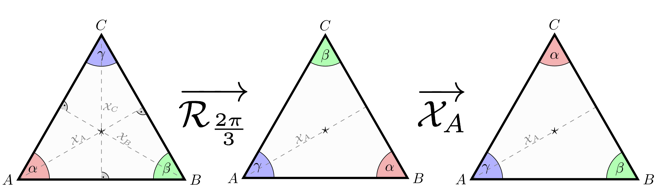
\includegraphics[width=5in]{VOLUMEN_1/02_Espacios_Lineales/Figuras/TriangRotRef.png}
\caption{Transformaciones  que dejan invariante un tri�ngulo equil�tero. Concatenaci�n de una rotaci�n, $\mathcal{R}_{\frac{2 \pi}{3}}$ con una reflexi�n, $\mathcal{X}_{A}$,  respecto a un plano que pasa por $A$}
\label{TriangRotRef}
\end{center}
\end{figure}
\begin{enumerate}
  \item Construya la tabla de multiplicaci�n para $\textbf{\em G}_{\triangle}$, vale decir $\textbf{\em G}_{\triangle}=\left\{ \mathcal{I}, \left\{\mathcal{R}_{i}\right\}, \left\{\bar{\mathcal{R}}_{j}\right\}, \left\{\mathcal{X}_{k}\right\} \right\}$ y la operaci�n es concatenaci�n tal y como mostramos en la figura \ref{TriangRotRef}. Donde $\mathcal{I}$ es la operaci�n identidad, $\left\{\mathcal{R}_{i}\right\}$ es un conjunto de rotaciones en sentido horario, mientras que $\left\{\bar{\mathcal{R}}_{j}\right\}$ es un conjunto de rotaciones en el sentido antihorario, y $\left\{\mathcal{X}_{k}\right\}$ el conjunto de las reflexiones que dejan invariante el tri�ngulo.
  \item Muestre que el conjunto de estas operaciones forman el grupo: $\textbf{\em G}_{\triangle}$.  
  
\item Identifique cada una de las $\mathcal{R}_{i}$ y $\bar{\mathcal{R}}_{j},$ y muestre adem�s, que forman un subgrupo c�clico de orden 3. De igual modo identifique las reflexiones y muestre que, cada una de las reflexiones y la identidad, $\left\{\mathcal{I}, \mathcal{X}_{i}\right\}$, forman tambi�n un subgrupo c�clico, pero de orden 2.
  \item Considere las siguientes matrices:
\[
\mathbb{I}= \left(\begin{array}{cc}1 & 0 \\0 & 1\end{array}\right)\,, \quad 
\mathbb{A} = \left(\begin{array}{cc} -\frac{1}{2} & \frac{\sqrt{3}}{2} \\ \\ -\frac{\sqrt{3}}{2} & -\frac{1}{2}\end{array}\right)\,, \quad
\mathbb{B} = \left(\begin{array}{cc} -\frac{1}{2} & -\frac{\sqrt{3}}{2} \\ \\ \frac{\sqrt{3}}{2} & -\frac{1}{2}\end{array}\right) \,,
\]
\[
\mathbb{C}= \left(
\begin{array}{cc}
-1 & 0 \\
0 & 1\end{array}\right)\,, \quad 
\mathbb{D} = \left(
\begin{array}{cc} 
\frac{1}{2} & -\frac{\sqrt{3}}{2} \\ \\ 
-\frac{\sqrt{3}}{2} & -\frac{1}{2}\end{array}\right) \,, \quad
\mathbb{E} = \left(
\begin{array}{cc} 
\frac{1}{2} & \frac{\sqrt{3}}{2} \\ \\ 
\frac{\sqrt{3}}{2} & -\frac{1}{2}\end{array}\right) \,.
\]
Muestre que forman grupo bajo la multiplicaci�n de matrices y que ese grupo es isomorfo a $\textbf{\em G}_{\triangle}$. 

\item Considere el conjunto de permutaciones de 3 objetos y la operaci�n composici�n de permutaciones que discutimos como ejemplo en la secci�n \ref{EjemploGrupo}. ?` Es ese grupo isomorfo a $\textbf{\em G}_{\triangle}$? Justifique su respuesta.   
\end{enumerate}

\item Considere las siguientes funciones:
\[
f_{1}(x)= x\,, \quad f_{2}(x)= \frac{1}{x}\,, \quad f_{3}(x)=  \frac{1}{1-x}\,, \quad 
f_{4}(x)=  \frac{x-1}{x}\,, \quad f_{5}(x)=  1-x\,, \quad f_{6}(x)=  \frac{x}{x-1}\,.
\]
Muestre que forman grupo bajo la operaci�n: $f_{i}(x) \odot f_{j}(x)= f_{i}(f_{j}(x))$, y que ese grupo es isomorfo a $\textbf{\em G}_{\triangle}$, del ejercicio anterior.  


\item  Definamos una operaci�n binaria $\blacksquare$ como: 
\[ 
x\ \blacksquare\ y=x+y+\alpha xy \,,
\] 
con $x,y,\alpha\in\mathds{R}$ y adem�s $\alpha\neq0$.
\begin{enumerate}
\item  Demuestre que $\blacksquare$ es asociativa.
\item  Muestre que $\blacksquare$ genera un grupo en $\left\{  \mathds{R}-
\left(  \frac{-1}{\alpha}\right)  \right\}$. Es decir, $\forall\,\, x,y\in\mathds{R}\,\,\wedge \,\,  x\neq\frac{-1}{\alpha}, y\neq\frac{-1}{\alpha}$, entonces: $x\ \blacksquare\ y$ forma un grupo.
\end{enumerate}

\item  Muestre que el siguiente conjunto de transformaciones en el plano $xy$ forman un grupo y construya su tabla de multiplicaci�n.
\begin{enumerate}
\item $I=\left\{ x\rightarrow x  \,\, \wedge \,\, y\rightarrow y \right\}$.

\item $I=\left\{ x\rightarrow-x \,\, \wedge \,\, y\rightarrow-y \right\} $.

\item $I_{x}=\left\{ x\rightarrow-x \,\, \wedge \,\, y\rightarrow y \right\} $.

\item $I_{y}=\left\{ x\rightarrow x \,\, \wedge \,\, y\rightarrow-y \right\} $.
\end{enumerate}

\item Considere un conjunto $\textbf{\em S}$ conformado �nicamente por n�meros reales positivos. Consideremos las siguientes reglas sobre $\textbf{\em S}$: Por ``suma" de dos n�meros entenderemos su producto  en el sentido usual, y el ``producto" de un elemento $r\in\textbf{\em S}$  y un n�mero real $\lambda$ entenderemos $r$ elevado a la potencia  de $\lambda$, en el sentido usual �$\textbf{\em S}$ es un espacio vectorial?

\item Considere el conjunto de vectores en el plano conformado por  vectores localizados en el origen y cuyos puntos finales permanecen siempre en el primer cuadrante �Este conjunto es un espacio vectorial?

\item Muestre que tambi�n ser�n espacios vectoriales:
\begin{enumerate}
\item  El  conjunto de todas las funciones  $f=f(x)$ definidas en $x=1$ con $f\left(  1\right) =0$.  Si $f\left( 1\right)=c$ �Tendremos igual un espacio vectorial? �Por qu�?
\item  Los vectores $\left( x,y,z\right)  \in \textbf{\em V}^{3}$ tal que sus componentes satisfacen el siguiente sistema de ecuaciones lineales:
\begin{align*}
a_{11}x+a_{12}y+a_{13}z  &  =0\\
a_{21}x+a_{22}y+a_{23}z  &  =0\\
a_{31}x+a_{32}y+a_{33}z  &  =0 \,.
\end{align*}
\end{enumerate}


%
%%%%%%%%%
\item Sea $\mathcal{P}_{n}$ el conjunto de todos los polinomios de grado $n,$ en $x,$ con coeficientes reales:
\[
\left| {p}_{n}\right> \rightleftharpoons p(x)=a_{0}+a_{1}x +a_{2}x^{2} +\dots +a_{n-1}x^{n-1}=\sum_{i=0}^{n-1}a_{i}x^{i}\,.
\]

\begin{enumerate}
\item  Demostrar que $\mathcal{P}_{n}$ es un espacio vectorial respecto a la suma de polinomios y a la multiplicaci�n de polinomios por un n�mero (n�mero real).

\item  Si los coeficientes $a_{i}$ son enteros �$\mathcal{P}_{n}$ ser� un espacio vectorial? �Por qu�?

\item �Cu�l de los siguientes subconjuntos de $\mathcal{P}_{n}$ es un subespacio vectorial?

\begin{enumerate}
\item  El polinomio cero y todos los polinomios de grado $n-1$.

\item  El polinomio cero y todos los polinomios de grado par.

\item  Todos los polinomios que tienen a $x$ como un factor (grado $n>1$).

\item  Todos los polinomios que tienen a $x-1$ como un factor.
\end{enumerate}
\end{enumerate}

%
%%%%%%%%%
\item Un subespacio $\mathcal{P}$ es generado por: 
$\left| {x}_1 \right> =x^{3}+2x+1\,, \,\, \left| {x}_2 \right> =x^{2}-2\,, \,\, \left| {x}_3\right> =x^{3}+x $
�Cu�l(es) de los siguientes polinomios pertenece al subespacio  
$\mathcal{P}$?
\begin{enumerate}
\item $x^{2}-2x+1$.
\item $x^{4}+1$.
\item $-\frac12x^{3}+\frac52x^{2}-x-1$.
\item $x-5$.
\end{enumerate}

\item Resuelva los ejercicios anteriores utilizando {\bf Maxima}.

\end{enumerate}


\section{Espacios m�tricos, normados y con producto interno}

En est� secci�n vamos a introducir una funci�n de distancia, de manera que si tenemos un par de puntos o elementos de un espacio vectorial podemos hablar de que existe una cierta distancia entre ellos. Se dice que la funci�n distancia induce una topolog�a sobre el espacio vectorial. 

Comenzaremos definiendo el concepto de m�trica sobre espacios vectoriales y con esta estructura llegar a la noci�n de norma. 

\subsection{M�tricas y espacios m�tricos}
\label{EspaciosMetricos}
\index{Espacios vectoriales lineales!M�tricos}
\index{M�tricos!Espacios vectoriales lineales}
\index{M�trica}
\index{Distancia!Espacios vectoriales lineales}
\index{Espacios vectoriales lineales!Distancia}
La dotaci�n de propiedades en los espacios vectoriales lineales lo constituye la idea de m�trica o distancia entre sus elementos. El concepto de m�trica surge de la generalizaci�n de la idea de distancia entre dos puntos de la recta real.

Un espacio vectorial ser� m�trico si podemos definir una funci�n:  
\[
d:\textbf{\em V}\times\textbf{\em V}\rightarrow\mathds{R} \,\, /  \,\, \forall  \left| x \right> ,\left| y
\right> ,\left|  {z}\right> \in\textbf{\em V} \,,
\] 
tal que se cumple lo siguiente:
\begin{enumerate}
\item $d\left(  \left| x \right> ,\left|  {y} \right> \right)  \geq 0\,, \quad \mathrm{si}  \quad 
d\left(  \left| x \right> ,\left| y \right> \right) = 0 \,\, \Rightarrow \,\, \left| x \right> \equiv \left|  {y} \right>$.

\item $d\left(  \left| x \right> ,\left| y \right> \right)  \equiv d\left(  \left| y \right>, \left| x \right> \right)$.

\item $d\left(  \left| x \right> ,\left|  y\right> \right)  \leq d\left(  \left| x \right> ,\left| z\right> \right)  +
d\left(  \left| y \right> ,\left|  {z}\right> \right) $  (La desigualdad triangular).
\end{enumerate}

As�, diremos que $\left(\textbf{\em V}, \textbf{\em K}, \boxplus , d\right)  $ es un espacio vectorial lineal, m�trico.

Podemos enumerar algunos ejemplos de espacios m�tricos:

\begin{enumerate}

\item Espacios reales $\mathds{R}^{n}$. Aqu� indicaremos  los diferentes puntos del espacio por las coordenadas:  $(x_1, x_2, \dots, x_n)$, $(y_1, y_2, \dots, y_n)$, ...

\begin{enumerate}
\item  Para $\mathds{R}$, es decir la recta real, la definici�n de m�trica es:
$d\left(  \left| x \right> ,\left| y \right> \right)  \equiv \left|  x-y\right|$\,.

\item  Para $\mathds{R}^{2}$, es decir el plano, una definici�n de m�trica
es: $d\left(  \left| x \right> ,\left|  {y} \right> \right)  \equiv\sqrt{\left(  x_{1}-y_{1}\right)^{2}+\left( x_{2}-y_{2}\right)^{2}}$. 

Tambi�n podemos construir otra definici�n de m�trica como: 
$d \left(  \left| x \right> ,\left|
{y}\right> \right)  \equiv\left|  x_{1}-y_{1}\right|  +\left|x_{2}-y_{2}\right|$. La primera de estas m�tricas se conoce como m�trica eucl�dea y la segunda como m�trica Manhattan o m�trica de taxistas. Es claro como el mismo espacio vectorial genera varios espacios m�tricos, dependiendo de la definici�n de m�trica. Para estos casos particulares, las m�tricas ``miden'' el desplazamiento entre dos puntos de forma distinta: en aviones (m�trica eucl�dea) o veh�culos terrestre en ciudades. 

\item  En general para espacios  reales $\mathds{R}^{n}$ una posible
definici�n de m�trica ser�:
 \[ 
 d\left(  \left| x \right>,\left| y \right> \right)  \equiv
 \sqrt{\left(  x_{1} -y_{1}\right)^{2}+\left(  x_{2}-y_{2}\right)^{2}+\left(  x_{3} -y_{3}\right)^{2}+\cdots+\left(  x_{n}-y_{n}\right)^{2}}\,.
\]
Esta definici�n de m�trica, o distancia, no es m�s que una generalizaci�n del teorema de Pit�goras y se denomina ``distancia euclidiana''. 
\end{enumerate}

\item  Espacios unitarios $n-$dimensionales, o espacios  complejos,
$\mathds{C}^{n}$. La definici�n de distancia puede construirse
como:  
\[
d\left(  \left| x \right> ,\left|  {y}\right> \right)  \equiv 
\sqrt{\left|  x_{1}-y_{1}\right|^{2}+\left|x_{2}-y_{2}\right|^{2}+\left|  x_{3}-y_{3}\right|^{2}+\cdots+\left| x_{n}-y_{n}\right|^{2}}\,,
\]  
y es claro que se recobra la idea de distancia en el plano complejo: $d\left(  \left| x \right> ,\left| y\right> \right)  \equiv\left|  x-y\right|$.

\item  Para los espacios de funciones $\mathcal{C}_{\left[  a,b\right]}^{\infty}$ una posible definici�n de distancia ser�a: 
\[
d\left(\left|  {f}\right> ,\left|  {g}\right> \right) \equiv
\max_{t\in\left[  a,b\right]  }\left|  f(t)  -g\left(t\right)  \right| \,.
\]  
\item La m�trica trivial o discreta
\[
d \left( \left|x\right> ,\left|y\right> \right) =
\left\{
\begin{tabular}{cc}
1 & si  $\ x \neq y$ \\
0 & si  $\ x= y$
\end{tabular}
\right.
\]

\end{enumerate}

\subsection{Normas y espacios normados}
\label{EspaciosNormados}
\index{Norma!Espacios vectoriales lineales}
\index{Espacios vectoriales lineales!Norma}
\index{Espacios vectoriales lineales!Normados}
\index{Normados!Espacios vectoriales lineales}
La idea de distancia (o m�trica) es el equipamiento m�s elemental que uno le puede exigir a un espacio vectorial. Mucho m�s interesante a�n son aquellos espacios vectoriales que est�n equipados con la idea de norma y, a partir de all�, se define la idea de distancia. La norma tiene que ver con el ``tama�o'' del vector y la m�trica tiene que ver con la distancia entre vectores. Cuando definimos la m�trica a partir de la norma, vinculamos las propiedades algebraicas del espacio con sus propiedades geom�tricas.

La norma, $\mathcal{N}\left(  \left|  v_{i}\right> \right) \equiv \left\|  \left|  v_{i}\right> \right\|$, de un espacio vectorial $\textbf{\em V}=\left\{  \left|{v}_{1}\right>, \left| v_{2}\right>, \left|  v_{3}\right>, \cdots , \left| v_{n}\right> \right\}$ ser� una funci�n:
\[
\mathcal{N}: \textbf{\em V}\rightarrow\mathds{R} \,\, /  \,\, \forall \ \left| v_{i}\right> \in\textbf{\em V} \,,
\] 
que cumple con:
\begin{enumerate}
\item  $\left\| \left|  v_{i}\right> \right\|  \geq0 \,, \quad \mathrm{si} \quad \left\|\left|v_{i}\right> \right\|=0
\,\, \Rightarrow \,\, \left|  v_{i}\right> \equiv\left|  {0}\right> $. 

\item $\left\|  \alpha\left|  v_{i}\right> \right\|  = \left|\alpha\right| \, \left\|  \left|  v_{i}\right> \right\|$. 

\item $\left\|  \left|{v}_{i}\right> +\left|{v}_{j} \right> \right\|  \leq\left\|  \left|{v}_{i} \right> \right\| +\left\|  \left|{v}_{j} \right> \right\|$ (Desigualdad triangular).
\end{enumerate}

\index{Norma!Distancia}
\index{Distancia!Norma}
\index{Banach!Stefan Banach}
\index{Banach!Espacios Vectoriales Normados}
La definici�n de norma induce una m�trica de la forma:
\[
d\left(\left| v_{i} \right>,\left|{v}_{j} \right> \right)\equiv \left\|  \left|{v}_{i}\right> -\left| v_{j}\right> \right\| \,.
\label{banach}
\]

Se denota en este caso un espacio vectorial normado\footnote{El concepto de espacio normado fue formulado en 1922 de manera independiente por: S. Banach, H. Hahn y N. Wiener.} como 
$\left(  \textbf{\em V}, \textbf{\em K}, \boxplus; \left\|
\cdot\right\|  \right) $, espacio que tambi�n es conocido como un espacio de Banach\footnote{{STEFAN BANACH} (1892 Kracovia, Polonia-1945 Lvov,Ucrania) Matem�tico polaco, uno de los fundadores del an�lisis funcional moderno, con sus mayores contribuciones a la teor�a de espacios topol�gicos. Hizo tambi�n importantes aportes a la teor�a de la medida, integraci�n y teor�a de conjuntos y series ortogonales.}. Esto significa que todo espacio normado es a su vez un espacio m�trico, pero es importante se�alar que no todo espacio m�trico es normado.

De la definici�n de distancia (\ref{banach}) resulta que la m�trica as� definida es invariante bajo traslaciones de vectores. Esto es, si; 
$\left|  {\tilde{x}}\right> =\left| x \right> +\left|  {a}\right> \,\, \wedge \,\,  
\left|  {\tilde{y}}\right> =\left| y \right> +\left|  {a}\right> $, entonces,  $ d\left(\left| x \right> ,\left| y\right> \right)  \equiv d\left(  \left|  {\tilde{x}}\right>,\left|  {\tilde{y}}\right> \right)$. Y adem�s es homog�nea: $d\left(\lambda\left| x \right> , \lambda \left| y\right> \right) = |\lambda| d\left(\left| x \right> ,\left| y\right> \right)$.


Como ejemplos de espacios normados podemos mostrar los siguientes:

\begin{enumerate}
\item  Los espacios reales, $\mathds{R}^{n}$ y los espacios complejos $\mathds{C}^{n}$.  Para estos espacios de Banach, la norma se define como:
\[
\left\|  \left| x \right> \right\|  =\sqrt{\left|x_{1}\right|^{2}+\left|  x_{2}\right|^{2}+\left|  x_{3}\right|
^{2}+\cdots+\left|  x_{n}\right|^{2}}=\left(  \sum_{i=1}^{n}\left| x_{i}\right|^{2}\right)^{\frac{1}{2}} \,.
\]

Para un espacio en $\mathds{R}^{3}$ se cumple que $\left\|\left| x \right> \right\|  = \sqrt{x_{1}^{2}+x_{2}^{2}+x_{3}^{2}}$, por lo tanto, la idea de norma generaliza la noci�n de ``tama�o'' del vector $\left| x \right>$. Es claro que la definici�n de distancia se construye a partir de la norma de la forma:
\[
d\left(  \left| x \right> ,\left| y \right>\right)  \equiv\left\|  \left| x \right> -\left|
{y}\right> \right\|  =\sqrt{\left|  x_{1}-y_{1}\right|^{2}+\left|  x_{2}-y_{2}\right|^{2}+\left|  x_{3}-y_{3}\right|^{2}
+\cdots+\left|  x_{n}-y_{n}\right|^{2}}\,.
\]

Este espacio se llama espacio normado euclidiano de dimensi�n $n$.

\item  Para el espacio lineal de matrices $n\times n$, reales o complejas, con el campo $\textbf{\em K}$ real o complejo, una definici�n de norma es:
\[
\left\|  M\right\|  =\sum_{a=1}^{m}\sum_{b=1}^{n}\left|  M_{ab}\right| \,,
\]
y la correspondiente definici�n de distancia:
\[
d\left(  \left| x \right> ,\left| y \right>\right)  \equiv\left\|  M-N\right\|  =\sum_{a=1}^{m}\sum_{b=1}^{n}\left|M_{ab}-N_{ab}\right| \,.
\]

\item  Para los espacios funcionales $\mathcal{C}_{\left[  a,b\right]
}^{\infty}$ una posible definici�n de norma ser�a:
\[
\left\|  \left|  {f}\right> \right\|  =\max_{t\in\left[a,b\right]  }\left|  f(t)  \right| \,,
\]
otra posible definici�n puede ser:
\[
\left\|  \left|  {f}\right> \right\|  =\sqrt{  \int_{a}^b\ \left|  f(t)  \right|^{2} \mathrm{d}t }\,.
\]
\end{enumerate}

\subsection{Espacios euclidianos}
\label{EspaciosHilbert}
\index{Interno!Producto}
\index{Producto interno!Espacios vectoriales lineales}
\index{Espacios vectoriales lineales!Producto interno}
\index{Hilbert!Espacios vectoriales lineales}
\index{Hilbert!David Hilbert}
\index{Espacios vectoriales lineales!Hilbert}
El siguiente paso en la construcci�n de espacios vectoriales m�s ricos es equiparlo con la definici�n de producto interno y a partir de esta definici�n construir el concepto de norma y con �ste el de distancia. La idea de producto interno generaliza el concepto de producto escalar de vectores en
$\mathds{R}^{3}$ e incorpora a los espacios vectoriales abstractos el concepto de ortogonalidad y descomposici�n ortogonal. Hist�ricamente, la teor�a de espacios vectoriales con producto interno es anterior a la teor�a de espacios m�tricos y espacios de Banach y se le debe a D.
Hilbert\footnote{{DAVID HILBERT }(1862 Kaliningrad, Rusia-1943 G�ttingen, Alemania) Matem�tico alem�n defensor de la axiom�tica como enfoque primordial de los problemas cient�ficos. Hizo importantes contribuciones en distintas �reas de la matem�tica, como: Invariantes, Campos de N�meros Algebraicos, An�lisis Funcional, Ecuaciones Integrales, F�sica-Matem�tica y C�lculo en
Variaciones.}.  Adicionalmente, la semejanza entre la geometr�a euclidiana y la geom�trica de
$\mathds{R}^{n}$ ha hecho que espacios en los cuales se puedan definir, distancia, �ngulos, a partir de una definici�n de producto interno, se denominen tambi�n espacios euclidianos.

\subsubsection{Producto interno}
\label{ProductoInterno}
\index{Interno!Producto}
\index{Producto interno}
En un espacio vectorial  $\textbf{\em V}=\left\{  \left| v_{1}\right>, \left| v_{2}\right>, \left| v_{3}\right>, \cdots , \left|  v_{n}\right> \right\}$, la definici�n del producto interno de dos vectores la denotaremos como $\left<{v}_{i}\right|\left.{v}_{j}\right>$ y es una aplicaci�n:  
\[
\mathcal{I}\left( \left| v_{i}\right>,\left| v_{j}\right>\right): 
\textbf{\em V} \times \textbf{\em V} \rightarrow \textbf{\em K}\,,  \,\, \forall \,\,\left| v_{i}\right> ,\left| v_{j}\right> \in\textbf{\em V}\,.
\]
Es decir, asocia a ese par de vectores con un elemento del campo $\textbf{\em K}$. 

Las propiedades que definen el producto interno son:
\begin{enumerate}
\item $\left<{v}_{i}\right|  \left. v_{i}\right> \equiv
\left\|  \left| v_{i}\right> \right\|^2  \,\, {\in} \,\, \textbf{\em K} \,\,\wedge\,\, \left<{v}_{i}\right|  \left.{v}_{i}\right> \geq0{\quad}\forall\ \left|  v_{i} \right> \in\textbf{\em V}\,,\quad \mathrm{si}
\quad \left<{v}_{i}\right|  \left. v_{i}\right> =0\,\, \Rightarrow \,\,\left| v_{i}\right> \equiv\left| {0}\right> $.

\item $\left<{v}_{i}\right|  \left.{v}_{j}\right> =\left<{v}_{j}\right|  \left. v_{i}\right> ^{\ast}{\quad}\forall\ \left| v_{i}\right> ,\left| v_{j}\right> \in\textbf{\em V}$.

\item $\left<{v}_{i}\right|  \left. \alpha{v}_{j}+\beta v_{k} \right> = 
\alpha \left<{v}_{i}\right|  \left.{v}_{j}\right> + \beta \left<{v}_{i}\right|  \left. v_{k}\right> 
\,\,\forall\,\, \left| v_{i}\right> ,\left|{v}_{j}\right> ,\left| v_{k}\right> \in\textbf{\em V} \,\, \wedge \,\, \alpha, \beta \, \in \, \textbf{\em K}$.

\item $\left<{\alpha{v}_{i}+\beta{v}_{j}}\right|  \left. v_{k}\right> =
\alpha^{\ast}\left<{v}_{i}\right|  \left.{v}_{k}\right> + \beta^{\ast} \left<{v}_{j}\right|  \left. v_{k}\right> 
\,\,\forall \,\, \left| v_{i}\right> ,\left|{v}_{j}\right>,\left| v_{k}\right> \in\textbf{\em V} \,\, \wedge \,\,  \alpha, \beta \, \in \, \textbf{\em K}$.

\item $\left<{v}_{i}\right|  \left.  {0}\right> =\left<{0}\right|  \left.{v}_{i}\right> =0$.
\end{enumerate}

\index{Producto interno!Norma}
\index{Norma!Producto interno}
\index{Producto interno!Distancia}
\index{Distancia!Producto interno}

Nota: la segunda y cuarta propiedad resultan del hecho de que si el campo  es complejo $\textbf{\em K}= \mathds{C}$, entonces:
\[
\left<\alpha{v}_{i}\right|  \left. \alpha{v}_{i}\right>=
\alpha^2\left<{v}_{i}\right|  \left.{v}_{i}\right>= 
i^2\left<{v}_{i}\right|  \left.{v}_{i}\right>= 
-\left<{v}_{i}\right|  \left.{v}_{i}\right>\,,
\]
lo cual contradice el hecho de que la norma tiene que ser positiva. Por eso la necesidad de tomar el complejo conjugado. Se dice entonces, que el producto escalar es {\it antilineal} respecto al primer factor y {\it lineal} respecto al segundo. 


A partir de la definici�n de producto interno se construyen los conceptos de norma y distancia:
\[
\left\|  \left| v_{i}\right> \right\|  =\sqrt{\left<{v}_{i}\right|  \left.  v_{i}\right> }\quad \mbox{y} \quad
d\left(  \left| v_{i}\right> ,\left| v_{j}\right> \right)  \equiv\left\|  \left| v_{i}\right> -\left| v_{j}\right> \right\|  =\sqrt{\left<{{v}_{i}-{v}_{j}}\right| \left.  {{v}_{i}-{v}_{j}}\right> }\,.
\]

\subsubsection{La desigualdad de Cauchy-Schwarz: los �ngulos entre vectores reales y complejos}
\label{DesigualdadCauchy-Schwarz}
\index{Cauchy-Schwarz!Desigualdad}
\index{Desigualdad!Cauchy-Schwarz}
Todo producto interno $\left<{v}_{i}\right|  \left.{v}_{j} \right> $ definido en un espacio vectorial normado $\textbf{\em V}=\left\{  \left|  v_{1}\right>, \left| v_{2}\right>, \left|  v_{3}\right>, \cdots ,\left|  v_{n}\right> \right\} $ cumple con la desigualdad de Cauchy-Schwarz:
\[
\left|  \left<{v}_{i}\right|  \left. v_{j}\right> \right|^{2}\leq\left<{v}_{i}\right|  \left.  v_{i}\right> \left<{v}_{j}\right|  \left.{v}_{j}\right>\quad \Longleftrightarrow \quad 
\left|  \left<{v}_{i}\right|  \left. v_{j}\right> \right|  \leq\left\|  \left| v_{i}\right> \right\|  \ \left\|  \left|{v}_{j}\right> \right\|\,.
\]
Es claro que si $\left|{v}_{i}\right> =\left|  {0}\right> \,\,\wedge \,\, \left| v_{j}\right> =\left|  {0}\right>$ se cumple la igualdad y es trivial la afirmaci�n. 

Para demostrar la desigualdad, tomemos dos vectores $\left|{v}_{i}\right> \,\, \wedge \,\, \left| v_{j}\right>$ cualesquiera, entonces podemos construir un tercero: $\left|{v}_{k}\right>=\alpha\left| v_{i}\right> +\beta\left|{v}_{j}\right>$  ($\alpha$ y  $\beta$ tendr�n valores particulares), por lo tanto:
\[
\left<{v}_{k}\right|  \left. v_{k}\right>  \equiv \left<\alpha{{v}_{i}+\beta v_{j}}\right|  \left.  \alpha{v}_{i}+{\beta v_{j}}\right> \geq 0 \,,
\]
esto significa que:
\begin{align*}
\left<\alpha{{v}_{i}+\beta v_{j}}\right|  \left.  \alpha{v}_{i} +{\beta v_{j}}\right>  &  =\left<\alpha{v}_{i}\right|
\left.  \alpha{v}_{i}\right> +\left<\alpha{v}_{i}\right| \left.  {\beta v_{j}}\right> +\left<{\beta v_{j}}\right|
\left.  \alpha{v}_{i}\right> +\left<{\beta v_{j}}\right| \left.  {\beta v_{j}}\right> \geq0\\
&  =\left|  \alpha\right|^{2}\left< v_{i}\right|  \left.  v_{i}\right> +\alpha^{\ast} \beta\left<{v}_{i}\right|  \left.  v_{j}\right> +{\beta}^{\ast}\alpha\left<{v}_{j}\right|  \left. v_{i}\right> +\left|  {\beta}\right|^{2}\left< v_{j}\right|  \left.  v_{j}\right> \geq 0 \,.
\end{align*}

Si $\alpha=\left<{v}_{j}\right|  \left. v_{j}\right>$,  se tiene que:
\begin{eqnarray*}
\left<{v}_{j}\right|  \left. v_{j}\right> \left< v_{i}\right|  \left.  v_{i}\right> &+&{\beta}\left< v_{i}\right|  \left.  v_{j}\right> +{\beta}^{\ast}\left<{v}_{j}\right|  \left.  v_{i}\right> +\left| {\beta}\right|^{2}\geq0 \\ 
\left<{v}_{j}\right|  \left. v_{j}\right> \left< v_{i}\right|  \left.  v_{i}\right> &\geq &-{\beta}\left<{v}_{i}\right|  \left.  v_{j}\right> - {\beta}^{\ast}\left<{v}_{j}\right|  \left.  v_{i}\right> - \left|{\beta}\right|^{2} \,,
\end{eqnarray*}
seguidamente seleccionamos: $\beta=-\left<{v}_{j}\right|  \left. v_{i}\right>$, y por lo tanto: ${\beta}^{\ast}=-\left<{v}_{i}\right|  \left. v_{j}\right>$,  consecuentemente:
\begin{eqnarray*}
\left<{v}_{j}\right|  \left. v_{j}\right> \left< v_{i}\right|  \left.  v_{i}\right> &\geq &
\left<{v}_{j}\right|  \left. v_{i}\right>\left<{v}_{i}\right|  \left.  v_{j}\right> +
\left< v_{i}\right|  \left. v_{j}\right>\left<{v}_{j}\right|  \left.  v_{i}\right> -
\left<{v}_{j}\right|  \left. v_{i}\right>\left<{v}_{i}\right|  \left.
{v}_{j}\right> \\
\left<{v}_{j}\right|  \left. v_{j}\right> \left< v_{i}\right|  \left. v_{i}\right> &\geq &
\left< v_{i}\right|  \left. v_{j}\right> \left<{v}_{j} \right|  \left. v_{i}\right> =\left|  \left<{v}_{i} \right|  \left. v_{j}\right> \right|^{2} \,. \quad \quad \blacktriangleleft
\end{eqnarray*}

De la desigualdad de Cauchy-Schwarz y la definici�n de norma se desprende que:
\[
\frac{\left|  \left<{v}_{i}\right|  \left. v_{j}\right>\right|^{2}}{\left\|  \left| v_{i}\right> \right\|^{2}\left\|
\left|  v_{j}\right> \right\|^{2}}\leq1 \,\, \Rightarrow\,\, -1\ {\leq}\frac{\left|  \left<{v}_{i}\right|  \left.{v}_{j}\right> \right|  }{\left\|  \left| v_{i}\right>\right\|  \left\|  \left|  v_{j}\right> \right\|  }\leq1 \,,
\]
por lo tanto podemos definir el ``�ngulo'' entre los vectores abstractos
$\left| v_{i}\right> \,\,\wedge\,\,\left| v_{j}\right>$ como:
\[
\cos(\Theta_{\mathds{G}})=\frac{\left|  \left<{v}_{i}\right|  \left.{v}_{j}\right> \right|  }{\left\|  \left|  v_{i}\right> \right\|  \left\|  \left| v_{j}\right> \right\|  } \,,
\]
donde hemos denotado como $\Theta_{\mathds{G}}$ el �ngulo gen�rico que forman los vectores reales o complejos. 
 
Si estamos considerando espacios vectoriales reales  -en los cuales el campo corresponde a los n�meros reales- entonces el �ngulo definido entre vectores abstractos reales corresponde al que intuitivamente siempre hemos considerado para los vectores cartesianos y que discutimos en la secci�n \ref{ProductoEscalar1},  
\[
\cos(\Theta_{\mathds{R}})=\frac{\left|  \left<{v}_{i}\right|  \left.{v}_{j}\right> \right|  }{\left\|  \left|  v_{i}\right> \right\|  \left\|  \left| v_{j}\right> \right\|  }\,,  \quad \mathrm{con } \quad 0 \leq \Theta_{\mathds{R}} \leq \pi \,,
\]
donde se toma $\Theta_{\mathds{R}} = 0$ para vectores colineales y $\Theta_{\mathds{R}} = \pi$ para vectores opuestos (antilineales). Si bien es cierto que esta definici�n coincide con la de los vectores cartesianos, hay que resaltar que la estamos extendiendo para cualquier vector abstracto, vale decir: funciones reales, matrices, y todos los objetos matem�ticos que cumplan con las reglas para los espacios vectoriales expuestas en \ref{EspaciosVectoriales}. 

Para el caso de espacios vectoriales complejos la situaci�n es m�s sutil y significa definir un �ngulo entre dos vectores abstractos y complejos, sin embargo podemos abordar el problema suponiendo:
\begin{enumerate}
  \item un espacio complejo $n-$dimensional de $n-$uplas de n�meros complejos $\left| z \right> \leftrightarrow (z_{1}, z_{2}, \cdots z_{n}) $ asociado (isomorfo) a un espacio vectorial real de $2n$ dimensiones, con vectores representados por $2n-$uplas de n�meros reales $\left|w\right> \leftrightarrow (\mathrm{Re}(z_{1}), \mathrm{Re}(z_{2}), \cdots \mathrm{Re}(z_{n}), \mathrm{Im}(z_{1}),\mathrm{Im}(z_{2}), \cdots \mathrm{Im}(z_{n}) )$, donde hemos representado $\mathrm{Re}(z_{j})$ y $\mathrm{Im}(z_{j})$ como las partes reales e imaginarias de $z_{j}$, respectivamente o,  
  \item directamente a partir de una definici�n de producto interno entre vectores complejos implementado por: $\left<{w}_{i}\right|  \left.{v}_{j}\right> = \sum_{j=1}^{n} {w}^{*}_{j} v_{j}$.
\end{enumerate}
Ambas aproximaciones no son del todo independientes pero igualmente justificadas\footnote{Scharnhorst, K. (2001). Angles in complex vector spaces. \textit{Acta Applicandae Mathematica}, \textbf{69}(1), 95-103.}. 

Consideremos el segundo caso, esto es: directamente a partir de una definici�n de producto interno entre vectores complejos. Para este caso consideramos un �ngulo complejo, y $\cos(\Theta_{\mathds{C}})$ una funci�n de variable compleja, que puede ser expresada en su forma polar como:
\[
\cos(\Theta_{\mathds{C}})=\frac{\left|  \left<{v}_{i}\right|  \left.{v}_{j}\right> \right|  }{\left\|  \left|  v_{i}\right> \right\|  \left\|  \left| v_{j}\right> \right\|  }  \,\, \Rightarrow \,\, 
\cos(\Theta_{\mathds{C}})= \rho \, \mathrm{e}^{ \phi}\,,  \quad \mathrm{con } \quad 
\rho = |\cos(\Theta_{\mathds{C}})| < 1\,.
\]

Entonces podemos asociar $\rho = \cos(\Theta_{H})$ y definir $\Theta_{H}$, en el rango $0 \leq \Theta_{H} \leq \pi/2$, como el \textit{�ngulo herm�tico} entre los vectores complejos $\left| v_{i} \right>$ y $\left| v_{j} \right>$. Mientras que $\phi$, definido en $-\pi \leq \phi \leq \pi$, corresponde al pseudo �ngulo de Kasner, que representa la orientaci�n o rotaci�n del �ngulo herm�tico y no tiene mayor significado al cuantificar el �ngulo entre esos dos vectores. Esta diferencia de significados puede intuirse cuando  multiplicamos $\left| v_{i} \right>$ y $\left| v_{j} \right>$, por una constante compleja: $\left| \tilde{v}_{i} \right> \rightarrow \alpha_{i} \left| v_{i} \right>$ y comprobamos que el �ngulo $\Theta_{H}$ permanece inalterado y no as� el �ngulo de Kasner\footnote{Puede consultarse Reju, V. G., Koh, S. N., y Soon, Y. (2009). An algorithm for mixing matrix estimation in instantaneous blind source separation. \textit{Signal Processing}, \textbf{89}(9), 1762-1773.}. 

\subsubsection{Teoremas del coseno y de Pit�goras}
\label{TeoremaCoseno}
\index{Teorema del!Coseno}
\index{Coseno!Teorema del}
\index{Teorema de!Pit�goras}
\index{Pit�goras!Teorema de}
A partir de la definici�n de norma se obtiene:
\[
\begin{array}{rl}
\left\|  \left|v_{i}\right> -\left|v_{j}\right>\right\| ^{2}= & \left<{{v}_{i} -{v}_{j}}\right|  \left.  {{v}_{i} -{v}_{j}}\right> =\left<{v}_{i}\right|  \left. v_{i} \right> -\left<{v}_{i}\right|  \left.v_{j}\right> -\left<{v}_{i}\right|  \left.v_{j}\right> ^{\ast} +\left<{v}_{j}\right|  \left. v_{j}\right>   \\
       =& \left<{v}_{i}\right|  \left.v_{i}\right> +\left<{v}_{j}\right|  \left. v_{j}\right>   -2 \, \mathrm{Re}\left(\left<{v}_{i}\right|  \left. v_{j}\right> \right) \,,
\end{array}
\]
con lo cual hemos generalizado el teorema del coseno para un espacio vectorial abstracto: 
\[
\left\|  \left|v_{i}\right> -\left|v_{j}\right>\right\|^{2}=
\left\|  \left|v_{i}\right> \right\|^{2} +\left\|  \left|v_{j}\right> \right\|^{2} -2\left\|  \left|{v}_{i}\right> \right\|  \left\|  \left| v_{j}\right> \right\|  \cos(\Theta_{\mathds{G}}) \, .
\]

De tal forma que para espacios vectoriales reales tendremos: 
\[
\left\|  \left| v_{i}\right> -\left| v_{j}\right>\right\|^{2}=
\left\|  \left| v_{i}\right> \right\|^{2} +\left\|  \left| v_{j}\right> \right\|^{2} -2\left\|  \left|{v}_{i}\right> \right\|  \left\|  \left| v_{j}\right> \right\|  \cos(\Theta)\,, \quad \mathrm{con } \quad 0 \leq \Theta \leq \pi \,,
\]
y para espacios vectoriales complejos: 
\[
\left\|  \left| v_{i}\right> -\left| v_{j}\right>\right\|^{2}=
\left\|  \left| v_{i}\right> \right\|^{2}+\left\|  \left| v_{j}\right> \right\|^{2} -2\left\|  \left|{v}_{i}\right> \right\|  \left\|  \left| v_{j}\right> \right\|  \cos(\Theta_{H}) \cos(\phi)\,, \quad \mathrm{con} \quad 0 \leq \Theta_{H} \leq \pi/2 \,.
\]

Para el caso que los vectores $\left| v_{i}\right> \,\,\wedge\,\, \left|{v}_{j}\right>$ sean ortogonales, esto es $\left<{v}_{i}\right|  \left. v_{j}\right> =0$, tendremos el teorema de Pit�goras generalizado: 
\[
\left\|  \left| v_{i}\right> -\left| v_{j}\right>\right\|^{2} \equiv \left\|  \left| v_{i}\right> +\left| v_{j}\right>\right\|^{2}=\left\|  \left| v_{i}\right> \right\|^{2}+\left\|  \left| v_{j}\right> \right\|^{2}\,.
\]

Veamos algunos ejemplos de espacios vectoriales con producto interno.

\begin{enumerate}
\item  Espacios euclidianos reales, $\mathds{R}^{n}$ y espacios euclidianos complejos
$\mathds{C}^{n}$.

Los vectores en estos espacios euclidianos  pueden ser representados por 
$\left| x \right> =\left(x_{1},x_{2},\cdots x_{n}\right) \,\,\wedge\,\, \left| y \right> =\left(  y_{1},y_{2},\cdots,y_{n}\right)  $ y \textbf{el producto interno} queda definido por:
\[
\left<{x}\right|  \left.  {y}\right> =x_{1}^*
y_{1}+x_{2}^*y_{2}+x_{3}^*y_{3},\cdots x_{n}^*y_{n}=\sum_{i=1}^{n}x_{i}^*y_{i} \,,
\]
es claro que esta definici�n de producto interno coincide, para $\mathds{R}^{2}$
(y $\mathds{R}^{3}$) con la idea de producto escalar convencional que consideramos en las secciones \ref{ProductoEscalar1} y \ref{ProductoEscalar2}, vale decir:
\[
\left.
\begin{array}
[c]{c}
{\bf{a}}=a_{x}{\mathbf{i}} +a_{y}{\mathbf{j}}\\
\\
{\bf{b}}=b_{x}{\mathbf{i}} +b_{y}{\mathbf{j}}
\end{array}
\right\} \,\, \Rightarrow \,\, {\bf{a}} \cdot {\bf{b}}=a_{x}b_{x}+a_{y}b_{y} \,.
\]

Ahora bien, el lector puede comprobar que para vectores en $\mathds{R}^{2}$ tambi�n se puede proveer una definici�n de producto interno:
\[
{\bf{a}}\circledast{\bf{b}}=2a_{x}b_{x}+a_{x}b_{y}+a_{y}b_{x}+a_{y}b_{y} \,,
\]
igualmente v�lida, con lo cual es claro que en un mismo espacio vectorial pueden coexistir diferentes productos internos. 

Por su parte, la \textbf{norma} es:
\[
\left\|  \left| x \right> \right\|  =\sqrt{\left< {x}\right|  \left.  {x}\right> }=\sqrt{x_{1}^{2}+x_{2}^{2}+x_{3}^{2},\cdots+x_{n}^{2}}=\sqrt{\sum_{i=1}^{n}x_{i}^{2}} \,.
\]

La \textbf{distancia} tambi�n recupera la idea intuitiva de distancia euclidiana:
\begin{align*}
d\left(  \left| x \right> ,\left| y \right>\right)   &  \equiv\left\|  \left| x \right> -\left| {y}\right> \right\|  =\sqrt{\left<{x-y}\right| \left.  {x-y}\right> }\\
         & \\
d\left(  \left| x \right> ,\left| y \right> \right)   &  = \sqrt{\left(  x_{1}-y_{1}\right)^{2}+\left(  x_{2} -y_{2}\right)^{2}+\left(  x_{3}-y_{3}\right)^{2}+\cdots+\left( x_{n}-y_{n}\right)^{2}} \,.
\end{align*}
El teorema del coseno queda como:
\[
\sum_{i=1}^{n}\left(  x_{i}+y_{i}\right)^{2}=\sum_{i=1}^{n}x_{i}^{2} +\sum_{i=1}^{n}y_{i}^{2}+2 \sqrt{\sum_{i=1}^{n}x_{i}^{2}} \  \sqrt{\sum_{i=1}^{n}y_{i}^{2}} \  \cos(\Theta) \,,
\]
mientras que el teorema de Pit�goras es:
\[
\sum_{i=1}^{n}\left(  x_{i}+y_{i}\right)^{2}=\sum_{i=1}^{n}x_{i}^{2} +\sum_{i=1}^{n}y_{i}^{2}\,,
\]
es obvio que para $\mathds{R}^{2}$ tanto el teorema del coseno como el teorema de Pit�goras retoman su forma tradicional.

Finalmente la desigualdad de Cauchy-Schwarz se expresa de la siguiente manera:
\[
\left|  \left<{x}\right|  \left.  {y}\right>\right|  \leq \left\|  \left| x \right> \right\|  \ \left\|\left| y \right> \right\| 
\,\, \Rightarrow \,\,
\left|  \sum_{i=1}^{n}x_{i}y_{i}\right|^{2}\leq  \sum_{i=1}^{n}x_{i}^{2} \ \sum_{i=1}^{n}y_{i}^{2} \,.
\]

\item  Para los espacios de funciones continuas $\mathcal{C}_{\left[a,b\right]  }^{\infty}$ una posible definici�n de \textbf{producto interno} ser�a:
\[
\left<{f}\right|  \left.  {g}\right>  = \int_a^b\mathrm{d}x\ f^{\ast}\left(x\right)  \ g\left(x\right) \,,
\]
de la cual se deriva la expresi�n para la \textbf{norma}:
\[
\left\|  \left|  {f}\right> \right\|^{2}=\left<{f}\right|  \left.  {f}\right> =\int_a^b \mathrm{d}x\ \left|  f(x)  \right|^{2}\,.
\]

La \textbf{distancia} entre funciones quedar� definida como:
\begin{align*}
d\left(  \left|  {f}\right> ,\left|  {g}\right> \right)   &  \equiv\left\|  \left|  {f}\right> -\left|{g}\right> \right\|  \equiv
\sqrt{\left<{f-g}\right|  \left.  {f-g}\right> }=
\sqrt{\left<{f}\right|  \left.  {f}\right>  -\left<{f}\right|\left.  {g}\right> -\left<{f}\right|  \left.{g}\right> ^{\ast}+\left<{g}\right|  \left.{g}\right> }\\
& \\
d\left(  \left|  {f}\right> ,\left|  {g}\right>\right)   &  =\sqrt{\int_a^b \mathrm{d}x\ \left| f(x)  -g(x)  \right|^{2}} \\
& \\
&  =\sqrt{\int_a^b \mathrm{d}x\ \left|f(x)  \right|^{2}  -2\operatorname{Re}\left(  \int_a^b \mathrm{d}x\ f^{\ast}(x)  \ g(x)\right)  +\int_a^b \mathrm{d}x\ \left|  g\left(x\right)  \right|^{2}}\,.
\end{align*}

El teorema del coseno puede ser escritos como:
\begin{align*}
\int_a^b \mathrm{d}x\ \left|  f(x) +g(x)  \right|^{2}  &  =
\int_a^b \mathrm{d}x\ \left|  f(x)  \right|^{2}+\int_a^b\mathrm{d}x\ \left|  g(x)  \right|^{2}\\
&  
+2\left(  \int_a^b \mathrm{d}x\ \left|  f\left(x\right)  \right|^{2}\right)  ^{\frac{1}{2}}\left(  \int_a^b\mathrm{d}x\ \left|  g(x)  \right|^{2}\right)
^{\frac{1}{2}}\cos(\Theta) \,,
\end{align*}
donde:
\[
\cos(\Theta)=\frac{\int_a^b \mathrm{d}x\ f^{\ast}\left( x\right)  \ g(x)  }{\left(  \int_a^b \mathrm{d}x\ \left|  f(x)  \right|^{2}\right)  ^{\frac{1}{2}
}\left(  \int_a^b \mathrm{d}x\ \left|  g\left( x\right)  \right|^{2}\right)  ^{\frac{1}{2}}} \,. 
\]

Y como era de esperarse el teorema de Pit�goras queda:
\[
\int_a^b \mathrm{d}x\ \left|  f(x) +g(x)  \right|^{2}=
\int_a^b \mathrm{d}x\ \left|  f(x)  \right|^{2}+\int_a^b \mathrm{d}x\ \left|  g(x)  \right|^{2} \,,
\]
para funciones $f(x)  $ y $g(x)  $ ortogonales, mientras que para este caso, la desigualdad de Cauchy-Schwarz se expresa:
\[
\left|  \int_a^b \mathrm{d}x\ f^{\ast}(x) \ g(x)  \right|^{2}\leq   \int_a^b  \mathrm{d}x\ \left|  f(x)  \right|^{2} \ \int_a^b \mathrm{d}x\ \left|  g(x)\right|^{2}\,.
\]
\end{enumerate}

\subsection{{\color{Fuchsia}Ejemplos}} 

\begin{enumerate}
\item Como vimos en la secci�n anterior, en el campo de los n�meros complejos el valor absoluto de $z=z+iy$ es $|z|=\sqrt{x^2+y^2}$. La m�trica que podemos asociar a este espacio vectorial viene dada por:
\[
d\left(  \left| z_1 \right> ,\left| z_2 \right>\right) \equiv \left\|  \left| z_1 \right> -\left|z_2\right> \right\|  =
\sqrt{\left<{z_1-z_2}\right|\left.  {z_1-z_2}\right> }= \sqrt{(x_1-x_2)^2+(y_1-y_2)^2} \,,
\]
con: $\left| z_1 \right>=x_1+iy_1$ y $\left| z_2\right>=x_2+iy_2$. 


\item  Consideramos el espacio vectorial de polinomios  de grado $g\leq n$ definidos en el intervalo $\left[ 0,1\right] $ o en el intervalo $\left[ -1,1\right]$ seg�n el caso. Suponiendo las siguientes definiciones de producto interno en $ \mathcal{P}^{n}$:
\[
\left<{q}_{n}\right. \left|{p}_{n}\right> = \int_{-1}^{1}p(x)q(x)\mathrm{d}x \quad \text{y} \quad 
\left<{q}_{n}\right. \left|{p}_{n}\right> = \int_{0}^{1}p(x)q(x)\mathrm{d}x \,.
\]
Vamos a encontrar la distancia y el �ngulo entre los vectores: $\left|{x}_1 \right> = x(x-1)$ y $\left|{x}_2\right> =x$.

En general, la definici�n de distancia es:
\[
d\left( \left|{x}_1\right>,\left|{x}_2\right> \right)=\sqrt{\left< {x}_2-{x}_1 \right. \left|{x}_2-{x}_1\right>}\,,
\]
por lo tanto para $\left<{q}_{n}\right. \left|{p}_{n}\right>  = \int_{-1}^{1}p(x)q(x)\mathrm{d}x$ la distancia ser�:
\[
\sqrt{\left< {x}_2-{x}_1\right. \left|{x}_2-{x}_1\right> } =
\sqrt{\int_{-1}^{1}\left[ x(x-1)-x\right]^{2}\mathrm{d}x} = \frac{1}{15}\sqrt{690} \,,
\]
y para $ \left<{q}_{n}\right. \left|{p}_{n}\right>  = \int_{0}^{1}p(x)q(x)\mathrm{d}x$, ser�:
\[
\sqrt{\left< {x}_2-{x}_1\right. \left|{x}_2-{x}_1\right> }=
\sqrt{\int_{0}^{1} \left( x(x-1)-x\right)^{2}\mathrm{d}x} = \frac{2}{15}\sqrt{30} \,.
\]

Con respecto a los �ngulos:
\[
\theta=\arccos \left( \frac{\left< {x}_1\right. \left|{x}_2 \right> }{\sqrt{ \left< {x}_1\right. \left|{x}_1 \right> } \sqrt{\left< {x}_2\right. \left|x_{2}\right> }}\right)\,.
\]

Para $\left<{q}_{n}\right. \left|{p}_{n} \right>  = \int_{-1}^{1}p(x)q(x)\mathrm{d}x$ tenemos:

\begin{align*}
\theta & =\arccos\left( \frac{\left< {x}_1\right. \left| {x}_2 \right> }{ \sqrt{\left< {x}_1\right. \left| {x}_1 \right> }\sqrt{\left< {x}_2\right. \left| {x}_2 \right> }}\right) =
\arccos \left(\frac{\int_{-1}^{1}\left( x(x-1)\right) x \ \mathrm{d}x}{\sqrt{ \int_{-1}^{1}\left( x(x-1)\right)^{2}\mathrm{d}x}\sqrt{\int_{-1}^{1} x^{2}\mathrm{d}x}}\right) \\
& \\
& =\arccos\left( -\frac{1}{12}\sqrt{15}\sqrt{6}\right) =2.4825 \text{ rad} \,.
\end{align*}
Para $\left<{q}_{n}\right. \left|{p}_{n}\right> = \int_{0}^{1}p(x)q(x)\mathrm{d}x$
\begin{align*}
\theta & =\arccos\left( \frac{\left< {x}_1\right. \left| {x}_2\right> }{\sqrt{\left< {x}_1\right. \left| {x}_1 \right> }\sqrt{\left< {x}_2\right. \left| {x}_2 \right> }}\right) =
\arccos\left(\frac{\int_{0}^{1}\left( x(x-1)\right) \left( x\right) \mathrm{d}x}{\sqrt{\int_{0}^{1}\left( x(x-1)\right) ^{2}\mathrm{d}x}\sqrt{\int_{0}^{1} x^{2} \mathrm{d}x}}\right) \\
& \\
& =\arccos\left( -\frac{1}{12}\sqrt{15}\sqrt{2}\right) =2.4825 \text{ rad}  
\qquad \text{�El mismo �ngulo!}
\end{align*}

\end{enumerate}

\newpage
\subsection{{\color{red}Practicando con Maxima}} 
\index{Espacios vectoriales con Maxima}
\index{MaximaEspaciosVectoriales}

\subsubsection{Espacios y subespacios vectoriales}

Sea el espacio vectorial $\textbf{\em V}=\textbf{\em K}^n$, definido en 
$\textbf{\em K}=\mathds{R}$ y donde $n$ es un entero positivo. Consideremos el caso $n=4$.
El producto de un elemento de $\textbf{\em K}^4$, digamos $\left| x \right>=(x_1, x_2, x_3, x_4)$ por un escalar $\alpha \in \textbf{\em K}$ resulta en otro elemento de $\textbf{\em K}^4$. 

Primero introducimos los elementos como listas:

%%%%%% INPUT:
\begin{minipage}[t]{8ex}
{\color{red}\bf \begin{verbatim} (%i1) 
\end{verbatim}}
\end{minipage}
\begin{minipage}[t]{\textwidth}{\color{blue}
\begin{verbatim}
X:[x1,x2,x3,x4];Y:[y1,y2,y3,y4];Z:[z1,z2,z3,z4];
\end{verbatim}}
\end{minipage}

%%% OUTPUT:
\begin{math}\displaystyle \parbox{8ex}{\color{labelcolor}(\%o1) }
\left[ { x_1} , { x_2} , { x_3} , { x_4} \right] 
\end{math}

%%% OUTPUT:
\begin{math}\displaystyle \parbox{8ex}{\color{labelcolor}(\%o2) }
\left[ { y_1} , { y_2} , { y_3} , { y_4} \right] 
\end{math}

%%% OUTPUT:
\begin{math}\displaystyle \parbox{8ex}{\color{labelcolor}(\%o3) }
\left[ { z_1} , { z_2} , { z_3} , { z_4} \right] 
\end{math}


%%%%%% INPUT:
\begin{minipage}[t]{8ex}
{\color{red}\bf \begin{verbatim} (%i4) 
\end{verbatim}}
\end{minipage}
\begin{minipage}[t]{\textwidth}{\color{blue}
\begin{verbatim}
alpha*X=Y;
\end{verbatim}}
\end{minipage}

%%% OUTPUT:
\begin{math}\displaystyle \parbox{8ex}{\color{labelcolor}(\%o4) }
\left[ \alpha\,{ x_1} , \alpha\,{ x_2} , \alpha\,{ x_3} ,  \alpha\,{ x_4} \right] 
=\left[ { y_1} , { y_2} , { y_3} , { y_4} \right] 
\end{math}
\newline

El resultado es un elemento del espacio vectorial $\textbf{\em K}^4$.

La suma de $\left| x \right>=(x_1, x_2, x_3, x_4)$ y $\left| y \right>=(y_1, y_2, y_3, y_4)$ ser�:

%%%%%% INPUT:
\begin{minipage}[t]{8ex}
{\color{red}\bf \begin{verbatim} (%i5) 
\end{verbatim}}
\end{minipage}
\begin{minipage}[t]{\textwidth}{\color{blue}
\begin{verbatim}
X+Y=Z;
\end{verbatim}}
\end{minipage}

%%% OUTPUT:
\begin{math}\displaystyle \parbox{8ex}{\color{labelcolor}(\%o5) }
\left[ { y_1}+{ x_1} , { y_2}+{ x_2} , { y_3}+ { x_3} , { y_4}+{ x_4} \right] =\left[ { z_1} ,  { z_2} , { z_3} , { z_4} \right] 
\end{math}
\newline

con $(z_1 ,  z_2 ,  z_3,  z_4) \in \textbf{\em K}^4$. 

Podemos ver r�pidamente que el conjunto  de vectores que tienen la forma  $(x_1,  x_2,  x_3,  0)$ conforman un subespacio de  $\textbf{\em K}^4$, ya que:

%%%%%% INPUT:
\begin{minipage}[t]{8ex}
{\color{red}\bf \begin{verbatim} (%i6) 
\end{verbatim}}
\end{minipage}
\begin{minipage}[t]{\textwidth}{\color{blue}
\begin{verbatim}
map(":",[x4,y4,z4],[0,0,0]);
\end{verbatim}}
\end{minipage}

%%% OUTPUT:
\begin{math}\displaystyle \parbox{8ex}{\color{labelcolor}(\%o6) }
\left[ 0 , 0 , 0 \right] 
\end{math}

%%%%%% INPUT:
\begin{minipage}[t]{8ex}
{\color{red}\bf \begin{verbatim} (%i7) 
\end{verbatim}}
\end{minipage}
\begin{minipage}[t]{\textwidth}{\color{blue}
\begin{verbatim}
X:[x1,x2,x3,x4];Y:[y1,y2,y3,y4];Z:[z1,z2,z3,z4];
\end{verbatim}}
\end{minipage}

%%% OUTPUT:
\begin{math}\displaystyle \parbox{8ex}{\color{labelcolor}(\%o7) }
\left[ { x_1} , { x_2} , { x_3} , 0 \right] 
\end{math}

%%% OUTPUT:
\begin{math}\displaystyle \parbox{8ex}{\color{labelcolor}(\%o8) }
\left[ { y_1} , { y_2} , { y_3} , 0 \right] 
\end{math}

%%% OUTPUT:
\begin{math}\displaystyle \parbox{8ex}{\color{labelcolor}(\%o9) }
\left[ { z_1} , { z_2} , { z_3} , 0 \right] 
\end{math}


%%%%%% INPUT:
\begin{minipage}[t]{8ex}
{\color{red}\bf \begin{verbatim} (%i10) 
\end{verbatim}}
\end{minipage}
\begin{minipage}[t]{\textwidth}{\color{blue}
\begin{verbatim}
alpha*X+beta*Y=Z;
\end{verbatim}}
\end{minipage}

%%% OUTPUT:
\begin{math}\displaystyle \parbox{8ex}{\color{labelcolor}(\%o10) }
\left[ \beta\,{ y_1}+\alpha\,{ x_1} , \beta\,{ y_2}+\alpha
 \,{ x_2} , \beta\,{ y_3}+\alpha\,{ x_3} , 0 \right] =
 \left[ { z_1} , { z_2} , { z_3} , 0 \right] 
\end{math}
\newline

Para recobrar las variables $x_4,y_4,z_4$ escribimos:

%%%%%% INPUT:
\begin{minipage}[t]{8ex}
{\color{red}\bf \begin{verbatim} (%i11) 
\end{verbatim}}
\end{minipage}
\begin{minipage}[t]{\textwidth}{\color{blue}
\begin{verbatim}
kill(x4,y4,z4)$
\end{verbatim}}
\end{minipage}

%%%%%% INPUT:
\begin{minipage}[t]{8ex}
{\color{red}\bf \begin{verbatim} (%i12) 
\end{verbatim}}
\end{minipage}
\begin{minipage}[t]{\textwidth}{\color{blue}
\begin{verbatim}
X:[x1,x2,x3,x4];Y:[y1,y2,y3,y4];Z:[z1,z2,z3,z4];
\end{verbatim}}
\end{minipage}

%%% OUTPUT:
\begin{math}\displaystyle \parbox{8ex}{\color{labelcolor}(\%o12) }
\left[ { x_1} , { x_2} , { x_3} , { x_4} \right] 
\end{math}

%%% OUTPUT:
\begin{math}\displaystyle \parbox{8ex}{\color{labelcolor}(\%o13) }
\left[ { y_1} , { y_2} , { y_3} , { y_4} \right] 
\end{math}

%%% OUTPUT:
\begin{math}\displaystyle \parbox{8ex}{\color{labelcolor}(\%o14) }
\left[ { z_1} , { z_2} , { z_3} , { z_4} \right] 
\end{math}
\newline

Para calcular el producto interno entre vectores es necesario utilizar la librer�a {\bf eigen}.

%%%%%% INPUT:
\begin{minipage}[t]{8ex}
{\color{red}\bf \begin{verbatim} (%i15) 
\end{verbatim}}
\end{minipage}
\begin{minipage}[t]{\textwidth}{\color{blue}
\begin{verbatim}
load("eigen")$
\end{verbatim}}
\end{minipage}

%%%%%% INPUT:
\begin{minipage}[t]{8ex}
{\color{red}\bf \begin{verbatim} (%i16) 
\end{verbatim}}
\end{minipage}
\begin{minipage}[t]{\textwidth}{\color{blue}
\begin{verbatim}
innerproduct(X,Y);
\end{verbatim}}
\end{minipage}

%%% OUTPUT:
\begin{math}\displaystyle \parbox{8ex}{\color{labelcolor}(\%o16) }
{x_4}\,{y_4}+{ x_3}\,{y_3}+{x_2}\,{y_2}+ {x_1}\,{y_1}
\end{math}
\newline

Consideremos ahora  $\textbf{\em V}=\textbf{\em K}^n$, definido en $\textbf{\em K}=\mathds{C}$, con $n=3$. Por lo tanto, los vectores ser�n ahora de la siguiente forma: $z=(x_1+iy_1, x_2+iy_2, x_3+iy_3)$. 

%%%%%% INPUT:
\begin{minipage}[t]{8ex}
{\color{red}\bf \begin{verbatim} (%i17) 
\end{verbatim}}
\end{minipage}
\begin{minipage}[t]{\textwidth}{\color{blue}
\begin{verbatim}
Z1:[x1+%i*y1,x2+%i*y2,x3+%i*y3]; Z2:[u1+%i*v1,u2+%i*v2,u3+%i*v3];
\end{verbatim}}
\end{minipage}

%%% OUTPUT:
\begin{math}\displaystyle \parbox{8ex}{\color{labelcolor}(\%o17) }
\left[ i\,{y_1}+{ x_1} , i\,{ y_2}+{ x_2} , i\,{ y_3}+{ x_3} \right]
\end{math}

%%% OUTPUT:
\begin{math}\displaystyle \parbox{8ex}{\color{labelcolor}(\%o18) }
\left[ i\,{ v_1}+{ u_1} , i\,{ v_2}+{ u_2} , i\, { v_3}+{ u_3} \right] 
\end{math}
\newline

Y los escalares de la forma $\alpha=a+ib$.

%%%%%% INPUT:
\begin{minipage}[t]{8ex}
{\color{red}\bf \begin{verbatim} (%i19) 
\end{verbatim}}
\end{minipage}
\begin{minipage}[t]{\textwidth}{\color{blue}
\begin{verbatim}
alpha:a+%i*b;
\end{verbatim}}
\end{minipage}

%%% OUTPUT:
\begin{math}\displaystyle \parbox{8ex}{\color{labelcolor}(\%o19) }
i\,b+a
\end{math}
\newline

El producto por el escalar $\alpha$ es:

%%%%%% INPUT:
\begin{minipage}[t]{8ex}
{\color{red}\bf \begin{verbatim} (%i20) 
\end{verbatim}}
\end{minipage}
\begin{minipage}[t]{\textwidth}{\color{blue}
\begin{verbatim}
Z3:alpha*Z1;
\end{verbatim}}
\end{minipage}

%%% OUTPUT:
\begin{math}\displaystyle \parbox{8ex}{\color{labelcolor}(\%o20) }
\left[ \left(i\,b+a\right)\,\left(i\,{ y_1}+{ x_1}\right) , 
 \left(i\,b+a\right)\,\left(i\,{ y_2}+{ x_2}\right) , \left(i\, b+a\right)\,\left(i\,{ y_3}+{ x_3}\right) \right] 
\end{math}

%%%%%% INPUT:
\begin{minipage}[t]{8ex}
{\color{red}\bf \begin{verbatim} (%i21) 
\end{verbatim}}
\end{minipage}
\begin{minipage}[t]{\textwidth}{\color{blue}
\begin{verbatim}
map(rectform,Z3);
\end{verbatim}}
\end{minipage}

%%% OUTPUT:
\begin{math}\displaystyle \parbox{8ex}{\color{labelcolor}(\%o21) }
\left[ i\,\left(a\,{y_1}+b\,{x_1}\right)-b\,{y_1}+a\,
 {x_1} , i\,\left(a\,{y_2}+b\,{x_2}\right)-b\,{y_2}+a
 \,{x_2} , i\,\left(a\,{y_3}+b\,{x_3}\right)-b\,{y_3}+a\,{ x_3} \right]
\end{math}

%%%%%% INPUT:
\begin{minipage}[t]{8ex}
{\color{red}\bf \begin{verbatim} (%i22) 
\end{verbatim}}
\end{minipage}
\begin{minipage}[t]{\textwidth}{\color{blue}
\begin{verbatim}
map(realpart,Z3),factor; map(imagpart,Z3),factor;
\end{verbatim}}
\end{minipage}

%%% OUTPUT:
\begin{math}\displaystyle \parbox{8ex}{\color{labelcolor}(\%o22) }
\left[ -\left(b\,{y_1}-a\,{x_1}\right) , -\left(b\,{y_2}-a\,{ x_2}\right) , -\left(b\,{y_3}-a\,{x_3} \right) \right] 
\end{math}

%%% OUTPUT:
\begin{math}\displaystyle \parbox{8ex}{\color{labelcolor}(\%o23) }
\left[ a\,{y_1}+b\,{x_1} , a\,{y_2}+b\,{x_2} , a\, {y_3}+b\,{x_3} \right] 
\end{math}
\newline

Calculemos ahora el producto interno: 
\[
Z_1 \cdot Z_2=(x_1+iy_1)^*(u_1+iv_1)+(x_2+iy_2)^*(u_2+iv_2)+(x_3+iy_3)^*(u_3+iv_3)\,.
\]


%%%%%% INPUT:
\begin{minipage}[t]{8ex}
{\color{red}\bf \begin{verbatim} (%i24) 
\end{verbatim}}
\end{minipage}
\begin{minipage}[t]{\textwidth}{\color{blue}
\begin{verbatim}
Z4:innerproduct(Z1,Z2);
\end{verbatim}}
\end{minipage}

%%% OUTPUT:
\begin{math}\displaystyle \parbox{8ex}{\color{labelcolor}(\%o24) }
\left({ v_3}-i\,{ u_3}\right)\,{ y_3}+\left({ v_2}-i\, {u_2}\right)\,{y_2}+\left({ v_1}-i\,{ u_1}\right)\, {y_1}+\left(i\,{ v_3}+{ u_3}\right)\,{x_3}+
\left(i\, {v_2}+{ u_2}\right)\,{ x_2}+\left(i\,{ v_1}+{ u_1} \right)\,{ x_1}
\end{math}

%%%%%% INPUT:
\begin{minipage}[t]{8ex}
{\color{red}\bf \begin{verbatim} (%i25) 
\end{verbatim}}
\end{minipage}
\begin{minipage}[t]{\textwidth}{\color{blue}
\begin{verbatim}
Re:map(realpart,Z4)$ Im:map(imagpart,Z4)$
\end{verbatim}}
\end{minipage}

%%%%%% INPUT:
\begin{minipage}[t]{8ex}
{\color{red}\bf \begin{verbatim} (%i26) 
\end{verbatim}}
\end{minipage}
\begin{minipage}[t]{\textwidth}{\color{blue}
\begin{verbatim}
Re+%i*Im;
\end{verbatim}}
\end{minipage}

%%% OUTPUT:
\begin{math}\displaystyle \parbox{8ex}{\color{labelcolor}(\%o26) }
i\,\left(-{ u_3}\,{ y_3}-{ u_2}\,{ y_2}-{ u_1}\, { y_1}+{ v_3}\,{ x_3}+{ v_2}\,{ x_2}+{ v_1}\, { x_1}\right)+{ v_3}\,{ y_3}+{ v_2}\,{ y_2}+{ v_1}
 \,{ y_1}+{ u_3}\,{ x_3}+{ u_2}\,{ x_2}+{ u_1}\,{ x_1}
\end{math}

%%%%%% INPUT:
\begin{minipage}[t]{8ex}
{\color{red}\bf \begin{verbatim} (%i27) 
\end{verbatim}}
\end{minipage}
\begin{minipage}[t]{\textwidth}{\color{blue}
\begin{verbatim}
kill(all)$
\end{verbatim}}
\end{minipage}

\subsubsection{Producto de polinomios}

Consideremos el siguiente producto escalar entre elementos de un espacio vectorial de polinomios:
\[
\left<p_i\right. \left|p_j\right> = \int_{a}^{b}p_i(x)p_j(x)\mathrm{d}x \,,
\]

Vamos a encontrar la distancia y el �ngulo entre los vectores $\left|{x}_1 \right> = x(x-1)$ y $\left|{x}_2\right> =x$ en dos intervalos diferentes: $\left[ 0,1\right] $ y $\left[ -1,1 \right]$

Debemos introducir los objetos a multiplicar:

%%%%%% INPUT:
\begin{minipage}[t]{8ex}
{\color{red}\bf \begin{verbatim} (%i1) 
\end{verbatim}}
\end{minipage}
\begin{minipage}[t]{\textwidth}{\color{blue}
\begin{verbatim}
P1:x*(x-1); P2:x;
\end{verbatim}}
\end{minipage}

%%% OUTPUT:
\begin{math}\displaystyle \parbox{8ex}{\color{labelcolor}(\%o1) }
\left(x-1\right)\,x
\end{math}

%%% OUTPUT:
\begin{math}\displaystyle \parbox{8ex}{\color{labelcolor}(\%o2) }
x
\end{math}
\newline

Ahora calculamos las distancias entre los vectores para ambos intervalos. Haremos gala de algunas posibilidades que ofrece el programa para escribir las expresiones. 

%%%%%% INPUT:
\begin{minipage}[t]{8ex}
{\color{red}\bf \begin{verbatim} (%i3) 
\end{verbatim}}
\end{minipage}
\begin{minipage}[t]{\textwidth}{\color{blue}
\begin{verbatim}
sqrt('integrate(((P1-P2)^2),x,-1,1))=sqrt(integrate(((P1-P2)^2),x,-1,1));
\end{verbatim}}
\end{minipage}

%%% OUTPUT:
\begin{math}\displaystyle \parbox{8ex}{\color{labelcolor}(\%o3) }
\sqrt{\int_{-1}^{1}{\left(\left(x-1\right)\,x-x\right)^2\;dx}}=
 \frac{\sqrt{46}}{\sqrt{15}}
\end{math}

%%%%%% INPUT:
\begin{minipage}[t]{8ex}
{\color{red}\bf \begin{verbatim} (%i4) 
\end{verbatim}}
\end{minipage}
\begin{minipage}[t]{\textwidth}{\color{blue}
\begin{verbatim}
sqrt('integrate(((P1-P2)^2),x,0,1))=sqrt(integrate(((P1-P2)^2),x,0,1));
\end{verbatim}}
\end{minipage}

%%% OUTPUT:
\begin{math}\displaystyle \parbox{8ex}{\color{labelcolor}(\%o4) }
\sqrt{\int_{0}^{1}{\left(\left(x-1\right)\,x-x\right)^2\;dx}}=
 \frac{2^{\frac{3}{2}}}{\sqrt{15}}
\end{math}
\newline

El �ngulo entre los polinomios definidos en el intervalo $\left[ -1,1 \right]$ es:

%%%%%% INPUT:
\begin{minipage}[t]{8ex}
{\color{red}\bf \begin{verbatim} (%i5) 
\end{verbatim}}
\end{minipage}
\begin{minipage}[t]{\textwidth}{\color{blue}
\begin{verbatim}
'integrate((P1*P2),x,-1,1)/(sqrt('integrate((P1*P1),x,-1,1))*
sqrt('integrate((P2*P2),x,-1,1)));
\end{verbatim}}
\end{minipage}

%%% OUTPUT:
\begin{math}\displaystyle \parbox{8ex}{\color{labelcolor}(\%o5) }
\frac{\int_{-1}^{1}{\left(x-1\right)\,x^2\;dx}}{\sqrt{\int_{-1}^{1
 }{x^2\;dx}}\,\sqrt{\int_{-1}^{1}{\left(x-1\right)^2\,x^2\;dx}}}
 \end{math}

%%%%%% INPUT:
\begin{minipage}[t]{8ex}
{\color{red}\bf \begin{verbatim} (%i6) 
\end{verbatim}}
\end{minipage}
\begin{minipage}[t]{\textwidth}{\color{blue}
\begin{verbatim}
ev(%,integrate);
\end{verbatim}}
\end{minipage}

%%% OUTPUT:
\begin{math}\displaystyle \parbox{8ex}{\color{labelcolor}(\%o6) }
-\frac{\sqrt{15}}{2^{\frac{3}{2}}\,\sqrt{3}}
 \end{math}

%%%%%% INPUT:
\begin{minipage}[t]{8ex}
{\color{red}\bf \begin{verbatim} (%i7) 
\end{verbatim}}
\end{minipage}
\begin{minipage}[t]{\textwidth}{\color{blue}
\begin{verbatim}
acos(%),numer;
\end{verbatim}}
\end{minipage}

%%% OUTPUT:
\begin{math}\displaystyle \parbox{8ex}{\color{labelcolor}(\%o7) }
2.482534617763384
 \end{math}
\newline

Y ahora, el �ngulo entre los polinomios definidos en el intervalo $\left[ 0,1 \right]$:

%%%%%% INPUT:
\begin{minipage}[t]{8ex}
{\color{red}\bf \begin{verbatim} (%i8) 
\end{verbatim}}
\end{minipage}
\begin{minipage}[t]{\textwidth}{\color{blue}
\begin{verbatim}
'integrate((P1*P2),x,0,1)/(sqrt('integrate((P1*P1),x,0,1))*
sqrt('integrate((P2*P2),x,0,1)));
\end{verbatim}}
\end{minipage}

%%% OUTPUT:
\begin{math}\displaystyle \parbox{8ex}{\color{labelcolor}(\%o8) }
\frac{\int_{0}^{1}{\left(x-1\right)\,x^2\;dx}}{\sqrt{\int_{0}^{1}{x
 ^2\;dx}}\,\sqrt{\int_{0}^{1}{\left(x-1\right)^2\,x^2\;dx}}}
 \end{math}

%%%%%% INPUT:
\begin{minipage}[t]{8ex}
{\color{red}\bf \begin{verbatim} (%i9) 
\end{verbatim}}
\end{minipage}
\begin{minipage}[t]{\textwidth}{\color{blue}
\begin{verbatim}
ev(%,integrate);
\end{verbatim}}
\end{minipage}

%%% OUTPUT:
\begin{math}\displaystyle \parbox{8ex}{\color{labelcolor}(\%o9) }
-\frac{\sqrt{30}}{4\,\sqrt{3}}
 \end{math}

%%%%%% INPUT:
\begin{minipage}[t]{8ex}
{\color{red}\bf \begin{verbatim} (%i10) 
\end{verbatim}}
\end{minipage}
\begin{minipage}[t]{\textwidth}{\color{blue}
\begin{verbatim}
acos(%),numer;
\end{verbatim}}
\end{minipage}

%%% OUTPUT:
\begin{math}\displaystyle \parbox{8ex}{\color{labelcolor}(\%o10) }
2.482534617763384
 \end{math}


\begin{center}
{\color{red}\rule{15.8cm}{0.4mm}}
\end{center}


\subsection{{\color{OliveGreen}Ejercicios}}

\begin{enumerate}
%%%%%%%%% Ejercicio 1
\item Consideremos el espacio vectorial conformado por los vectores geom�tricos en $\mathds{R}^{3}$ �Ser�n espacios euclidianos para las siguientes definiciones de producto interno?
\begin{enumerate}
\item El producto de las longitudes de los vectores. 
\item El producto de las longitudes por el cubo del coseno del �ngulo entre ellos. 
\item El producto como dos veces el producto escalar usual entre vectores.
\end{enumerate}

%%%%%%%%% Ejercicio 2
\item  Considerando estas definiciones de producto interior en $\mathcal{P}_{n}$:
\[
a)\quad \left<{q}_{n}\right. \left|{p}_{n}\right> =\int_{-1}^{1}p(x)q(x)\mathrm{d}x\,, \qquad
b) \quad  \left<{q}_{n}\right. \left|{p}_{n}\right> =\int_{0}^{1}p(x)q(x)\mathrm{d}x \,.
\]
\begin{enumerate}
  \item Encuentre los �ngulos en el ``tri�ngulo'' formado por los vectores: $\left| x_1 \right>=1, \left| x_2 \right>=t, \left| x_3 \right>=1-t$.
  \item Encuentre la distancia y el �ngulo entre los siguientes pares de vectores en $\mathcal{P}_{3}$:
\begin{enumerate}
\item $\left| {x}_1\right> = 1; \quad \left|{x}_2\right> = x$.
\item $\left| {x}_1 \right>  = 2x;\quad \left|{x}_2\right> = x^{2}$.
\end{enumerate}
\end{enumerate}


%%%%%%%%% Ejercicio 3
\item Sea $\textbf{\em E}^\prime$ un subespacio euclidiano de dimensi�n $k$, $\textbf{\em E}^\prime  \subset \textbf{\em E}$,  y sea  
$\left| v \right>$ un vector que no necesariamente es un elemento 
$\textbf{\em E}^\prime$. Podemos plantearnos el problema de representar $\left| v \right>$ de la forma:
$\left| v \right>= \left| g \right>+\left| h \right> $;  donde $\left| g \right> \in \textbf{\em E}^\prime$ y $\left| h \right>$ es ortogonal a $\textbf{\em E}^\prime$. La existencia de la expansi�n anterior nos muestra que el espacio total $\textbf{\em E}$, de dimensi�n $n$, es la suma directa de los subespacios $\textbf{\em E}^\prime$ y su complemento ortogonal $\textbf{\em E}^\perp$ de dimensi�n $n-k$. 

Encuentre el vector $\left| v \right>$, como la suma del vector $\left| g \right>$, expandido por los vectores $\left| g_i \right>$, y el vector perpendicular $\left| h\right>$ cuando:
\begin{enumerate}
\item $\left| h \right>=(5,2,-2,2)\,,\, \left| g_1 \right>=(2,1,1,-\alpha)\,,\,
\left| g_2 \right>=(1,\beta,3,0)$.
\item $\left| h \right>=(-3,5,9,3)\,,\, \left| g_1 \right>=(1,1,1,\gamma)\,,\,
\left| g_2 \right>=(2\eta,-1,1,1)\,,\, \left| g_3 \right>=(2,-7\delta,-1,-1)$.
\end{enumerate}


%
%%%%%%%%%
\item  Sean $\left| p_{n} \right> = p(x) = \sum_{i=0}^{n-1}a_{i}x^{i}\,; \quad \left| {q}_{n} \right> =q(x)=\sum_{i=0}^{n-1}
b_{i}x^{i} \in \mathcal{P}_{n}$. Consid�rese la siguiente definici�n:
\[
\left< {q}_{n} \right. \left|{p}_{n}\right> \rightleftharpoons a_{0}b_{0}
+a_{1}b_{1}+a_{2}b_{2}+...+a_{n-1}b_{n-1}=\sum_{i=0}^{n-1}a_{i}b_{i}
\]

\begin{enumerate}
\item  Muestre que �sta es una buena definici�n de producto interno.

\item  Con esta definici�n de producto interior ?`Se puede considerar $\mathcal{P}_{n}$ un subespacio de $\mathcal{C}_{[a,b]}$? ?`Por qu�?
\end{enumerate}



%
%%%%%%%%% Ejercicio 4
\index{Cuaterni�n}
\item Los vectores en $\mathds{R}^{3}$ en coordenadas cartesianas los definimos como
${\bf a}= a^i \left|{e}_{i}\right \rangle = a_{x}{\bf {i}}+a_{y}{\bf {j}}+a_{z}{\bf {k}}$ y definimos una ``tabla de multiplicaci�n'' entre ellos
de la forma $\left<{e}^{i}\right.  \left| {e}_{j}\right> =
\delta_{j}^{i}$ con $i,j=1,2,3$, esto es:
\[
\begin{tabular}
[c]{|c|c|c|c|}
\hline
$\left<{e}^{i}\right.  \left|  {e}_{j}\right> $ &${\bf {i}}$ & ${\bf {j}}$ & ${\bf {k}}$\\\hline\hline
${\bf {i}}$ & $1$ & $0$ & $0$\\\hline
${\bf {j}}$ & $0$ & $1$ & $0$\\\hline
${\bf {k}}$ & $0$ & $0$ & $1$\\\hline
\end{tabular}
\]
Un cuaterni�n cartesiano puede escribirse de manera an�loga a los
vectores cartesianos, vale decir:
\[
\left|  {a}\right> =a^{\alpha}\left|  {q}_{\alpha}\right> =a^{0}+a^{i}\left|  {q}_{i}\right> =a_{0}
+a_{x}{\bf {i}}+a_{y}{\bf {j}}+a_{z}{\bf {k}} \,,
\]
con $\alpha=0,1,2,3$ y donde las $a^{i}$ (con $i=1,2,3$) son n�meros reales que representan las componentes vectoriales en coordenadas cartesianas de los cuaterniones,  mientras que la $a^{0},$ tambi�n un n�mero real se le llama componente escalar\footnote{Recuerde que estamos utilizando la convenci�n de Einstein en la cual: $c^{\alpha}\left|  {q}_{\alpha}\right> \equiv c^{0}+\sum_{j=1}^{3}c^{j}\left|  {q}_{j}\right> $. Es decir, hemos supuesto que: $\left|  {q}_{0}\right> \equiv1$, la unidad en los n�meros reales. Adicionalmente, n�tese que los �ndices griegos $\alpha,\beta,\cdots$ toman los valores $0,1,2,3$, mientras que los latinos que acompa�an a los vectores cartesianos toman los siguiente valores $j,k,l=1,2,3$.}. 

Los cuaterniones fueron inventados por el matem�tico irland�s William Rowan Hamilton  a mediados del siglo XIX, y por decirlo de alguna manera, son h�bridos o generalizaciones a un plano hipercomplejo. Un vector cartesiano es un cuaterni�n con la componente escalar nula. Hoy encontramos aplicaciones del �lgebra de cuaterniones en F�sica\footnote{Hace algunas d�cadas se dio una discusi�n sobre la importancia de utilizar esta representaci�n en F�sica Cu�ntica. Pueden consultar:
\begin{itemize}
  \item Berezin, A. V., Kurochkin, Y. A., \& Tolkachev, E. A. (1989). Quaternions in relativistic physics. Nauka i Tekhnika, Minsk.
  \item Girard, P. R. (1984). The quaternion group and modern physics. European Journal of Physics, 5(1), 25.
  \item Horwitz, L. P., \& Biedenharn, L. C. (1984). Quaternion quantum mechanics: second quantization and gauge fields. Annals of Physics, 157(2), 432-488.
\end{itemize}}
 y m�s recientemente ha tenido alguna utilizaci�n computaci�n gr�fica que discutiremos en el pr�ximo problema en el contexto del �lgebra geom�trica y las algebras de Grassman.

Bas�ndonos en este esquema podemos definir la ``tabla de multiplicaci�n'' para los cuaterniones cartesianos como:
\[
\begin{tabular}
[c]{|c||r|r|r|r|}\hline
$\left|  {q}_{i}\right> \odot\left|  {q}_{j}\right> $ & ${1}$ & $\left|  {q}_{1}\right> $ &$\left|  {q}_{2}\right> $ & $\left|  {q}_{3}\right>$\\\hline\hline
${1}$ & ${1}$ & $\left|  {q}_{1}\right> $ &$\left|  {q}_{2}\right> $ & $\left|  {q}_{3}\right>
$\\\hline
$\left|  {q}_{1}\right> $ & $\left|  {q}_{1}\right> $ & $-{1}$ & $\left|  {q}_{3}\right> $ &$-\left|  {q}_{2}\right> $\\\hline
$\left|  {q}_{2}\right> $ & $\left|  {q}_{2}\right> $ & $-\left|  {q}_{3}\right> $ & $-{1}$& $\left|  {q}_{1}\right> $\\\hline
$\left|  {q}_{3}\right> $ & $\left|  {q}_{3}\right> $ & $\left|  {q}_{2}\right> $ & $-\left|{q}_{1}\right> $ & $-{1}$\\\hline
\end{tabular}
\]

N�tese que por el hecho de que: 
\[\left|  {q}_{j}\right>\odot \left|  {q}_{j}\right> =-1\Rightarrow\left|  {q}_{1}\right> \odot\left|  {q}_{1}\right> =\left|{q}_{2}\right> \odot\left|  {q}_{2}\right> = \left|{q}_{3}\right> \odot\left|  {q}_{3}\right> =-1\,,
\]
se puede pensar que un cuaterni�n es la generalizaci�n de los n�meros complejos a m�s de una dimensi�n (un n�mero hipercomplejo), donde la parte imaginaria tendr�a tres dimensiones y no una como es costumbre. 

Esto es:
\[
\left|  {a}\right> = 
a^{\alpha}\left|  {q}_{\alpha}\right> =a^{0}\underset{{1}}{\underbrace{\left|  {q}_{0}\right> }}+a^{j}\left|  {q}_{j}\right> =
a^{0}+\underset{\text{``parte compleja''}}{\underbrace{a^{1}\left|  {q}_{1}\right> +a^{2}\left|  {q}_{2}\right> +a^{3}\left| {q}_{3}\right> }} \,.
\]

Siendo consistente con esa visi�n de generalizaci�n de un n�mero complejo, definiremos el conjugado de un cuaterni�n como: 
\[
\left| {b}\right> ^{\maltese}=b^{0}\left|  {q}_{0}\right> -b^{j}\left|  {q}_{j}\right> \,,
\]
con $\ j=1,2,3$. 

Es decir, en analog�a con los n�meros complejos el conjugado de un cuaterni�n cambia el signo de su ``parte compleja vectorial''. 

Igualmente, definiremos la suma entre cuaterniones de la siguiente manera:
\[
\left.
\begin{array}[c]{c}
\left|  {a}\right> =a^{\alpha}\left|  {q}_{\alpha }\right> \\
\\
\left|  {b}\right> =b^{\alpha}\left|  {q}_{\alpha}\right>
\end{array}
\right\} \,\, \Rightarrow \,\, \left|  {c}\right> =
c^{\alpha}\left|{q}_{\alpha}\right> = 
\left|  {a}\right> +\left|{b}\right> =
\left(  a^{\alpha}+b^{\alpha}\right)  \left| {q}_{\alpha}\right> \,\, \Rightarrow \,\,  c^{\alpha}=
\left(a^{\alpha}+b^{\alpha}\right) \,.
\]

Esto quiere decir que los vectores se suman componente a componente. Mientras que la multiplicaci�n por un escalar queda definida por $\alpha\left| {c}\right> =\alpha c^{\alpha}\left|  {q}_{\alpha }\right>$, es decir se multiplica el escalar por cada componente.

Con la informaci�n anterior, responda las siguientes preguntas:

\begin{enumerate}
\item  Compruebe si los cuaterniones, $\left|  {a}\right>$,  forman un espacio vectorial respecto a esa operaci�n  suma y esa multiplicaci�n por escalares, an�loga a la de los vectores en $\mathds{R}^{3}$ en coordenada cartesianas.

\item  Dados dos cuaterniones cualesquiera $\left|  {b}\right> \equiv\left( b^{0},{\bf b}\right) $ y $\left|  {r}\right> \equiv\left( r^{0}, {\bf r}\right) $, y su tabla de multiplicaci�n, muestre que el producto entre esos cuaterniones $\left| {d}\right> =\left|  {b}\right> \odot \left| {r}\right> $ podr� representarse como:
\[
\left|  {d}\right> =\left|  {b}\right> \odot \left| {r}\right> \longleftrightarrow \left(  d^{0}, {\bf d}\right)=
\left(  b^{0}r^{0} -{\bf b} \cdot {\bf r},\ r^{0} {\bf b} +b^{0}{\bf r} + {\bf b} \times {\bf r}\right) \,,
\]
donde $\cdot$ y $\times$ corresponden con los productos escalares y vectoriales tridimensionales de siempre.

\item Ahora con �ndices: dados $\left|  {b}\right> = b^{\alpha}\left|  {q}_{\alpha}\right> $ y $\left| {r}\right> =r^{\alpha}\left|  {q}_{\alpha}\right>$,  compruebe si el producto $\left|  {d}\right> =\left| {b}\right> \odot\left|  {r}\right> $ puede ser siempre escrito de la forma:
\[
\left|  {d}\right> = \left|  {b}\right> \odot \left|{r}\right> = a\left|  {q}_{0}\right> + {S}^{(\alpha j)}\delta_{\alpha}^{0}\left|  {q}_{j}\right> +A^{\left[  jk\right] i}b_{j}r_{k}\left|  {q}_{i}\right>\,.
\]  
donde $a$ representa un n�mero, $S^{\left(  \alpha j\right)  }\delta_{\alpha}^{0}$ (recuerde que los �ndices latinos toman los  valores $j,k,l=1,2,3$, mientras $\alpha = 0,1,2,3$),  donde $S^{\left(  ij\right)  }$ indica $S^{ji}=S^{ij}$, que la cantidad $S^{ij}$ es sim�trica, y por lo tanto $\left(  S^{\alpha j}\delta_{\alpha}^{0}+S^{j\alpha}\delta_{\alpha}^{0}\right)  \left|  {q}_{j}\right>$.  

Mientras $A^{\left[  jk\right]  i}$ representa un conjunto de objetos antisim�tricos en $j$ y $k$:\footnote{Para familiarizarse con las expresiones vectoriales con la notaci�n de �ndices puede consultar la secci�n \ref{AlgebraVectorialIndices}.}
\[
A^{\left[  jk\right]  i} \rightarrow A^{jki}=-A^{kji} \rightarrow
\left(  A^{jki}b_{j}r_{k}-A^{kji}b_{j}r_{k}\right) \left|  {q}_{i}\right> \,.
\]


\item Identifique las cantidades: $a$, $S^{\left(ij\right)}$ y $A^{\left[  jk\right]  i}$,  
 en t�rminos  de las componentes de los cuaterniones.
 
 \textquestiondown El producto de cuaterniones $\left|  {d}\right> =\left|  {a}\right>\odot\left|  {r}\right>$ ser� un vector, pseudovector o ninguna de las anteriores? Explique por qu�.

\item  Muestre que los cuaterniones pueden ser representados por matrices complejas $2 \times 2$ del tipo:
\[
\left|  {b}\right> \longleftrightarrow
\left(
\begin{array}
[c]{cc}
z & w\\
-{w}^* & {z}^*
\end{array}
\right)\,,
\]
donde $z,w$ son n�meros complejos.

\item  Muestre que una representaci�n posible para la base de cuaterniones es, la matriz unitaria $4x4$:
\[
\left|  {q}_{1}\right> =\left(
\begin{array}
[c]{cccc}
0 & 1 & 0 & 0\\
-1 & 0 & 0 & 0\\
0 & 0 & 0 & 1\\
0 & 0 & -1 & 0
\end{array}
\right)\,,\quad \left|  {q}_{2}\right> =\left(
\begin{array}
[c]{cccc}
0 & 0 & 0 & -1\\
0 & 0 & -1 & 0\\
0 & 1 & 0 & 0\\
1 & 0 & 0 & 0
\end{array}
\right)\,,\quad \left|  {q}_{3}\right> =\left(
\begin{array}
[c]{cccc}
0 & 0 & -1 & 0\\
0 & 0 & 0 & 1\\
1 & 0 & 0 & 0\\
0 & -1 & 0 & 0
\end{array}
\right) \,.
\]

\item  Compruebe si la siguiente es una buena definici�n de producto interno:
\[
\widetilde{\left<{a}\right.  \left|  {b}\right> }=\left|
{a}\right>^{\maltese}\odot\left|  {b}\right> \,.
\]

\item  Modifique un poco la definici�n anterior de tal forma que:
\[
\left<{a}\right.  \left|  {b}\right>  =\frac{1}{2}\left[
\widetilde{\left<{a}\right.  \left|  {b}\right> } -\left|{q}_{1}\right> \odot \widetilde{\left<{a}\right.  \left|  {b}\right> } \odot\left|  {q}_{1}\right> \right] \,,
\]
y compruebe si esta definici�n compleja del producto interno cumple con todas las propiedades. N�tese que un cuaterni�n de la forma $\left|{f}\right> =f^{0}+f^{1}\left| {q}_{1}\right>$ es un n�mero complejo convencional.

\item  Compruebe si la siguiente es una buena definici�n de norma para los cuaterniones:
\[
n(\left|  {b}\right> )=\left\|  \left|  {a}\right>\right\|  =\sqrt{\left<{a}\right.  \left|  {a}\right> }=\sqrt{\left|  {a}\right> ^{\maltese}\odot\left|{a}\right> } \,.
\]

\item  Compruebe si un cuaterni�n definido por:
\[
\overline{\left|  {a}\right> }=\frac{\left|  {a}\right>^{\maltese}}{\left\|  \left|  {a}\right> \right\|^{2}}\,,
\]
puede ser considerado como el inverso o elemento sim�trico de $\left|{a}\right>$, respecto a la multiplicaci�n $\odot$.

\item  Compruebe si los cuaterniones $\left|  {a}\right> $ forman un grupo respecto a una operaci�n multiplicaci�n $\odot$.

\item  Los vectores en $\mathds{R}^{3}$ en coordenadas cartesianas, $\left|{v}\right>$, pueden ser representados como cuaterniones, donde la parte escalar es nula $v^{0}=0\rightarrow \left| {v}\right>=v^{j}\left|  {q}_{j}\right>$. Compruebe si el siguiente producto conserva la norma:
\[
\left|  {v}^{\prime}\right> =\overline{\left|  {a} \right> }\odot\left|  {v}\right> \odot\left|{a}\right> \,. 
\]
Estos es: 
$ 
\left\|  \left| {v}^{\prime}\right> \right\|^{2}=\left(  v^{1^\prime}\right)^{2}+\left(  v^{2^\prime}\right) ^{2}+\left(v^{3^\prime}\right) ^{2}\equiv\left(  v^{1}\right)^{2}+\left(  v^{2}\right)
^{2}+\left(  v^{3}\right)^{2}=\left\|  \left|  {v}\right>\right\|  ^{2}\,.
$ 
\end{enumerate}
%\newpage

\item En el mismo esp�ritu de los cuaterniones considerados previamente estudiemos el siguiente problema.

%%%%%%%%%%%%%%%%%
\begin{figure}[h]
\begin{minipage}{7.5cm}

Consideremos otra vez el espacio $\mathds{R}^{3}$ expandido por la base ortonormal est�ndar $\left\{  \bf{i}, \bf{j}, \bf{k} \right\}$.

Supongamos en este espacio el producto de dos vectores $\bf{a}$ y $\bf{b}$ (o $\left|a\right>$ y $\left|b\right>$ en la notaci�n de vectores abstractos de Dirac) definido a la manera del \textit{�lgebra geom�trica}.  

Esto es:
\[
\left|a\right> \bigodot \left|b\right> \equiv \bf{a}\bf{b} = \bf{a}\cdot\bf{b} + \bf{a}\wedge\bf{b} \,,
\]
con  $\bf{a}\cdot\bf{b}$ el producto escalar est�ndar de $\mathds{R}^{3}$, representando la parte conmutativa de $\bf{a}\bf{b}$ y $\bf{a} \wedge \bf{b}$ su parte anticonmutativa. Esta �ltima parte se relaciona con el producto vectorial est�ndar de la representaci�n de Gibbs como: ${\bf a}\wedge{\bf b} = i \bf{a}\times\bf{b}$, con $ i = {\bf i} \wedge {\bf j} \cdot {\bf k}$ un pseudoescalar.


\end{minipage} \hfill 
\begin{minipage}{8.0cm} 
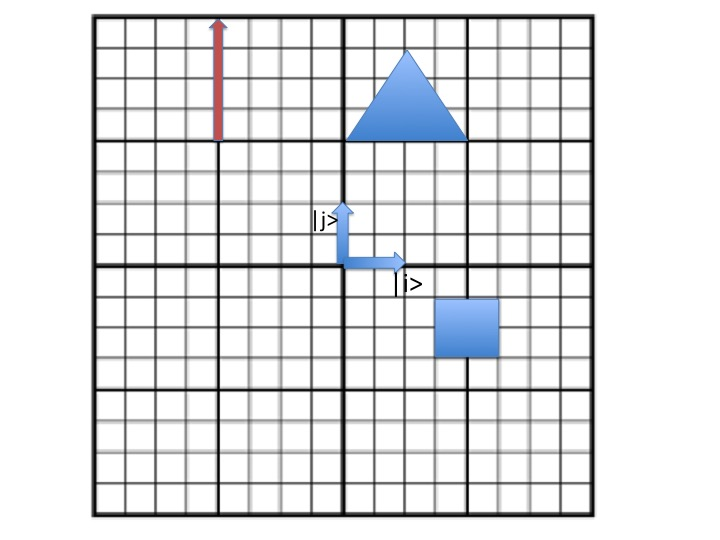
\includegraphics[height=2.3in,width=3.3in]{VOLUMEN_1/02_Espacios_Lineales/Figuras/FiguraCasitaPropuestos.jpg}
\caption{Se ilustran los vectores ortonormales est�ndares $\left\{ {\bf i}, {\bf j} \right\}$ y como siempre ${\bf k} = {\bf i} \times {\bf j} $.}
\label{FiguraAlgebraGeometrica}
\end{minipage}
\end{figure}
%%%%%%%%%%%%%%%%%
Este formalismo ha tenido cierto impacto en computaci�n gr�fica\footnote{Esta representaci�n para objetos f�sicos ha tenido cierto �xito en F�sica cl�sica y cu�ntica; se puede consultar:
\begin{itemize}
  \item Hestenes, D., \& Sobczyk, G. (2012). Clifford algebra to geometric calculus: a unified language for mathematics and physics (Vol. 5). Springer Science \& Business Media.
  \item Hestenes, D. (1971). Vectors, spinors, and complex numbers in classical and quantum physics. Am. J. Phys, 39(9), 1013-1027.
  \item Hestenes, D. (2003). Spacetime physics with geometric algebra. American Journal of Physics, 71(7), 691-714.  
  \item Dressel, J., Bliokh, K. Y., \& Nori, F. (2015). Spacetime algebra as a powerful tool for electromagnetism. Physics Reports, 589, 1-71.
\end{itemize}}-\footnote{Y equivalentemente, por isomorfismo $i=\sqrt{-1}$.}-\footnote{Pueden consultar 
\begin{itemize}
  \item  Goldman, R. (2002). On the algebraic and geometric foundations of computer graphics. ACM Transactions on Graphics (TOG), 21(1), 52-86.
  \item Hildenbrand (2011). From Grassmann's vision to geometric algebra computing. Springer Basel.
  \item Hildenbrand, D., Fontijne, D., Perwass, C., \& Dorst, L. (2004). Geometric algebra and its application to computer graphics. In Tutorial notes of the EUROGRAPHICS conference.
  \item Vince, J. (2008). Geometric algebra for computer graphics. Springer Science \& Business Media
\end{itemize} y las referencias all� citadas.} y lo vamos a utilizar para modelar transformaciones de objetos en el espacio. 

Considere el caso 2D representado en la figura \ref{FiguraAlgebraGeometrica},  en el formalismo de algebra geom�trica el objeto tri�ngulo lo asociamos con vector abstracto $\left| \bigtriangleup \right>$, mientras que el objeto cuadrado lo representaremos como $\left| \Box \right>$, y el tercer objeto por $\left| \Uparrow \right>$. 

Entonces:

\begin{enumerate}
  \item Exprese los vectores: $\left| \bigtriangleup \right>, \left| \Box \right>, \left| \Uparrow \right>$ en t�rminos de la base ortonormal est�ndar $\left\{  {\bf i}, {\bf j}, {\bf k} \right\}$ (o $\left|{ \rm i}\right>, \left|{ \rm j}\right>, \left|{ \rm k}\right> $) en el formalismo de �lgebra geom�trica.
  
  \item Exprese $\left| \bigtriangleup \right> \bigodot \left| \Uparrow \right>$ en t�rmino de la base geom�trica. Vale decir, si $\left|O_{g}\right> $ es un objeto geom�trico este podr�  representarse en t�rminos de una base: $\left| \epsilon \right>, \left| {\sigma} \right>, \left| B \right>, \left| i \right> $, donde $\left| \epsilon \right>$ es un escalar; $\left| {\sigma} \right>$ es un vector, $\left| B \right>$ un bivector y, finalmente $\left| i \right>$ un pseudoescalar.
  
  \item  Encuentre la norma de cada uno de ellos y la distancia entre  $\left| \bigtriangleup \right>$ y $\left| \Uparrow \right>$.
  
\item Considere ahora la operaci�n: $\mathbb{A}\left| \bigtriangleup \right> = \left| \tilde{\bigtriangleup} \right>$.

\begin{enumerate}
  \item Si $\mathbb{A}_{\left| {\rm j} \right>}$ es el operador reflexi�n respecto $\left| {\rm j} \right>$, exprese en t�rminos geom�tricos $\left| \tilde{\bigtriangleup} \right> = \mathbb{A}_{\left| {\rm j} \right>}\left| \bigtriangleup \right>$ y $\mathbb{A}_{\left| {\rm i} \right>}\left(\left| \bigtriangleup \right> \bigodot \left| \Uparrow \right>\right) $.
  
  \item Si $\mathbb{A}_{\theta, \left| B \right>}$ es el operador de rotaci�n alrededor de un bivector $\left| B \right>$ un �ngulo $\theta$. Encuentre $\mathbb{A}_{\pi/4, \left| B \right>}\left(\left| \bigtriangleup \right> \bigodot \left| \Uparrow \right>\right) $ con $\left| B \right> = \left|{\rm j}\right> + \left|{\rm k}\right>$.
\item �C�mo interpreta Ud. la ecuaci�n de autovalores $\mathbb{A}\left| \bigtriangleup \right> = 2 \left| \bigtriangleup \right>$?
\end{enumerate}  

 \item Considere el caso 3D en el cual  $\left| \hat{\bigtriangleup} \right>$ representa un tetraedro regular con la base representada por la figura \ref{FiguraAlgebraGeometrica} y $\left| \hat{\Box }\right>,$ un cubo, tambi�n con su base representada en el plano de la misma figura. 
  \begin{enumerate}
%%%  
  \item Exprese los vectores: $\left| \hat{\bigtriangleup} \right>, \left| \hat{\Box} \right>$ en t�rminos de la base ortonormal est�ndar $\left\{ {\bf i}, {\bf j}, {\bf k} \right\}$  y el formalismo de �lgebra geom�trica.
%%%
  \item  Exprese $\left(\left| \hat{\bigtriangleup} \right> \bigodot \left| \Uparrow \right>\right) \bigodot \left| \bigtriangleup \right> $ en t�rmino de la base geom�trica.
%%%
  \item Encuentre la norma de $\left| \hat{\bigtriangleup} \right>$ y la distancia entre  $\left| \hat{\bigtriangleup} \right>$ y $\mathbb{A}_{\pi/2, \left| -{\rm j} \right>}\left| \hat{\Box} \right>$.
%%
  \item Exprese $\left[\mathbb{A}_{\pi/2, \left| -{\rm j} \right>} ,\mathbb{B}_{\pi/4, \left| {\rm i} \right>} \right]\left| \hat{\Box} \right>$, con  $\left[\mathbb{A}_{\pi/2, \left| -{\rm j} \right>} ,\mathbb{B}_{\pi/4, \left| {\rm i} \right>} \right]= \mathbb{A}_{\pi/2, \left| -{\rm j} \right>} \mathbb{B}_{\pi/4, \left| {\rm i} \right>} -  \mathbb{B}_{\pi/4, \left| {\rm i} \right>} \mathbb{A}_{\pi/2, \left| -{\rm j} \right>}$.
\end{enumerate}
\end{enumerate}



%%%%%%%%%%%%%%%%%%
\item En Geometr�a Diferencial podemos considerar a $\mathds{R}^{3}$ como un conjunto de puntos (una variedad o espacio topol�gico), es decir, $\mathds{R}^{3}$ no es un espacio vectorial como se defini� con anterioridad. 
En un punto $q$ cualquiera podemos generar un plano $\mathds{R}^{2}$, entendido tambi�n como un conjunto de puntos, y definir el siguiente conjunto $T_q \mathds{R}^{2}=$ \{el conjunto de todos los vectores geom�tricos (flechas) con origen en  $q$  que son tangentes al plano $\mathds{R}^{2}$\}. Notemos que la idea la podemos extender para cualquier superficie, por ejemplo, una esfera $\mathds{S}^{2}$ (embebida en $\mathds{R}^{3}$) y sobre la esfera  seleccionar un punto arbitrario $q$. A partir de este punto $q$ generar un plano y construir el conjunto $T_q \mathds{S}^{2}=$ \{el conjunto de todos los vectores geom�tricos con origen en  $q$  que son tangentes a la esfera $\mathds{S}^{2}$\}.

\begin{enumerate}
\item �Es $T_q \mathds{R}^{2}$ un espacio vectorial?
\item Claramente podemos seleccionar otro punto arbitrario, pero diferente de $q$, digamos $p$ y construir el conjunto $T_p \mathds{R}^{2}$. �Son estos dos espacios isomorfos? 
\end{enumerate}

Consideremos ahora el conjunto de todas las funciones diferenciables
$f: \mathds{R}^{3} \,\,\rightarrow\,\, \mathds{R}$. Esto es, que existen todas las derivadas parciales en $q \in \mathds{R}^{3}$:
\[
\partial_x f(x^i)\,,\, \partial_y f(x^i)\,,\, \partial_z f(x^i)\,\, \in \,\,\mathds{R}
\,\, \forall\,\, (x^i) \,\, \in\,\, \mathds{R}^{3}\,.
\]
Note que hemos supuesto un sistema de coordenadas cartesiano $x^i=(x,y,z)$ en $\mathds{R}^{3}$ y que las derivadas son evaluadas en $q$. 

Consideremos el espacio tangente $T_q \mathds{R}^{3}$ en un punto $q$ arbitrario y  un vector $\left| u_q\right> \in T_q \mathds{R}^{3}$ con componentes $\left(u^1,u^2,u^3\right)$, podemos definir el siguiente operador (operador derivada direccional) en $q$ siguiendo a 
$\left| u_q\right>$:
\[ 
\left| U_q\right>= \left(u^1\partial_x+u^2\partial_y+u^3\partial_z\right)_q \,.
\]
Por lo tanto:
\[
\left| U_q\right> f \equiv \left(u^1\partial_x+u^2\partial_y+u^3\partial_z\right)_q f = u^1(\partial_xf)_{q} +u^2(\partial_yf)_{q} +u^3(\partial_zf)_{q} \,.
\]
Es  posible entonces construir el conjunto de los operadores derivadas direccionales que act�an sobre las funciones $f$:
\[
\mathcal{D}_q(\mathds{R}^{3})= \{ \left| U_q\right> =  \left(u^1\partial_x+u^2\partial_y+u^3\partial_z\right)_q \,\, \forall\,\, 
\left| u_q\right> \,\, \in \,\,T_q \mathds{R}^{3} \} \,.
\]
\begin{description}
\item[]
c) �Es $\mathcal{D}_q$ un espacio vectorial? 
\item[]
d) �Los espacios  $\mathcal{D}_q$  y $T_q \mathds{R}^{3}$ son isomorfos? 
\end{description}

\item Resuelva los problemas anteriores utilizando {\bf Maxima}. 

\end{enumerate}


\section{Variedades lineales}
\label{VariedadesLineales}
\index{Variedades lineales}

Resulta de gran inter�s construir subespacios vectoriales a partir de una cantidad de vectores $\{ \left| \mathrm{w}_{i}\right>\}$. En este caso diremos que los vectores generan una variedad lineal. Es decir, si tenemos una cantidad de vectores: $\{\left| \mathrm{w}_{1}\right>, \left| \mathrm{w}_{2}\right>, \left| \mathrm{w}_{3}\right>, \dots \}$ $\in \textbf{\em V}$, entonces una variedad lineal generada por este conjunto se entender� como el conjunto de todas las combinaciones lineales finitas:
\[
\alpha\left| \mathrm{w}_{1}\right>+\beta\left| \mathrm{w}_{2}\right>+\gamma\left| \mathrm{w}_{3}\right> +\cdots \,,
\]
donde los coeficientes: $\alpha, \beta, \gamma, \dots$ pertenecen al campo $\textbf{\em K}$. 

Se puede comprobar que esta variedad lineal es un subespacio de $\textbf{\em V}$. Claramente, todo subespacio que contenga los vectores $\{\left| \mathrm{w}_{1}\right>, \left| \mathrm{w}_{2}\right>, \left| \mathrm{w}_{3}\right>, \dots \}$ tambi�n contiene todas sus combinaciones lineales, por lo tanto, la variedad lineal generada de esta manera es el subespacio m�s peque�o que contiene al conjunto de estos vectores. 

Una variedad lineal sencilla de construir  en $\textbf{\em V}=\mathds{R}^{3}$ la constituye un par de vectores no colineales. La variedad lineal generada por estos dos vectores ser� el conjunto de todos los vectores paralelos al plano determinado por este par de vectores no colineales. Mientras que la variedad lineal generada por los vectores: $\{{\bf i}, {\bf j},{\bf k}\} \in \mathds{R}^{3}$  es el mismo espacio entero $\mathds{R}^{3}$.

Pasemos ahora a considerar el problema de construir una base para una variedad lineal y a partir de all� determinar la dimensi�n de la variedad.


\subsection{Dependencia/Independencia lineal}
\label{Dependencia lineal}
\index{Dependencia lineal}
\index{Independencia Lineal}

Siguiendo la misma l�nea de razonamiento que en las secciones \ref{IndependenciaVector3D} y \ref{IndependenciaVector3D2}, generalizamos el concepto de dependencia e independencia lineal de 
$\mathds{R}^{2}$ y $\mathds{R}^{3}$. As�:
\[
\left|  {0}\right> =C_{1}\ \left|  v_{1}\right> +C_{2}\ \left|  v_{2}\right> +C_{3}\ \left|  v_{3}\right> \cdots+C_{n}\ \left|  v_{n}\right>
=\sum_{i=1}^{n}C_{i}\ \left|  v_{i}\right> ,
\]
Las cantidades $C_{i}$ son llamados los coeficientes de la combinaci�n lineal. 

Podemos afirmar que:
\begin{itemize}
\item  Si esta ecuaci�n se cumple para alg�n conjunto de $\left\{
C_{i}\right\}  $ no nulos, se dir� que el conjunto de vectores
correspondiente $\left\{  \left|  v_{i}\right> \right\}  $ son
\textbf{linealmente dependientes.}

\item  Por el contrario, si esta ecuaci�n \textbf{s�lo} puede ser
satisfecha para todos los $C_{i}=0$,  entonces se dir� que el conjunto de
vectores correspondiente $\left\{\left| v_{i}\right>
\right\}  $ son \textbf{linealmente independientes.}
\end{itemize}
Notemos que la suma que aparece aqu� es necesariamente una suma finita, y cuando un determinado conjunto de vectores es linealmente dependiente, entonces uno de ellos se puede escribir como combinaci�n lineal de los dem�s.

\subsection{Bases de un espacio vectorial}
\label{BasesEspaciosVectoriales}
\index{Bases para Espacios vectoriales lineales}
\index{Espacios vectoriales lineales!Bases de}
Ahora bien, dado un espacio vectorial $\textbf{\em V}=\left\{  \left| v_{1}\right> ,\ \left|  v_{2}\right> ,\ \left| v_{3}\right> \cdots,\left|  v_{n}\right> \right\}  $, si encontramos que el conjunto de $\left\{  \left|  v_{n}\right> \right\}$ es linealmente dependiente, entonces siempre es posible despejar uno de los vectores en t�rminos de los dem�s, vale decir:
\[
\left|  v_{n}\right> =\bar{C}_{1}\ \left|  v_{1}\right> +\bar{C}_{2}\ \left|  v_{2}\right> +\bar{C}_{3}\ \left|  v_{3}\right> \cdots+\bar{C}_{n-1}\ \left| v_{n-1}\right> =\sum_{i=1}^{n-1}\bar{C}_{i}\ \left| v_{i}\right> \,.
\]

Seguidamente podemos proceder a comprobar si $\left\{  \left|  v_{1}\right> ,\ \left|  v_{2}\right> ,\ \left| v_{3}\right> \cdots,\left|  v_{n-1}\right> \right\}$ es un conjunto de vectores linealmente independientes, es decir: $\bar{C}_{1}\ =\bar{C}_{2}\ =\bar{C}_{3}\ =\cdots=\bar{C}_{n-1} =0$. 

En caso de no serlo se procede otra vez a despejar uno de los vectores en t�rminos de los anteriores y aplicar el criterio de independencia lineal:
\begin{align*}
\left|  v_{n-1}\right>  &  =\tilde{C}_{1}\ \left| v_{1}\right> +\tilde{C}_{2}\ \left|  v_{2}
\right> +\tilde{C}_{3}\ \left|  v_{3}\right> \cdots+\tilde{C}_{n-2}\ \left|  v_{n-2}\right> =\sum_{i=1}^{n-2}\tilde{C}_{i}\ \left|  v_{i}\right> \,,
\end{align*}
nuevamente se comprueba si se cumple:  $\tilde{C}_{1}  =\tilde{C}_{2}\ =\tilde{C}_{3}\ =\cdots=\tilde{C}_{n-2}=0$. 

En caso contrario, se repite este procedimiento hasta encontrar un conjunto: 
$\left\{  \left|{v}_{1}\right> ,\ \left|  v_{2}\right> ,\ \left| v_{3}\right> \cdots,\left|  v_{n-j}\right> \right\}$  de vectores linealmente independientes. Esto es:
$ \breve{C}_{1}\ =\breve{C}_{2}\ =\breve{C}_{3}\ =\cdots=\breve{C}_{n-j} =0$.

Por lo tanto:
\begin{align*}
\left|  v_{n-j+1}\right>  &  =\breve{C}_{1}\ \left| v_{1}\right> +\breve{C}_{2}\ \left|  v_{2}\right> +\breve{C}_{3}\ \left|  v_{3}\right> \cdots+\breve{C}_{n-j}\ \left|  v_{n-j}\right> =\sum_{i=1}^{n-j}\ \breve{C}_{i}\ \left|  v_{i}\right> \,.
\end{align*}

Diremos entonces que $\left\{  \left|  v_{1}\right>, \left|  v_{2}\right>, \left|  v_{3}\right>, \cdots,\left|  v_{n-j}\right> \right\}$ forman una base para el espacio vectorial  $\textbf{\em V}$. 

Es importante se�alar, que la dimensi�n de $\textbf{\em V}$ ser� el n�mero de vectores linealmente independientes, que para este caso ser�: dim$\textbf{\em V}= n-j$. 

Entonces,  se puede comprobar que, dado un vector arbitratio $\left| x \right> \in\textbf{\em V}$, se tiene que:
\[
\left| x \right> =\sum_{i=1}^{n-j}\ C_{i}\ \left|
{v}_{i}\right>  \,\,\forall\,\, \left| {x}\right> \in\textbf{\em V}\,,
\]
y el conjunto $\left\{ C_{1},C_{2},C_{3},\cdots C_{n-j}\right\}$ ser�
�nico. 

Diremos que el n�mero m�nimo de vectores: 
$\left|  v_{1}\right> ,\ \left|  v_{2}\right>,\ \left|  v_{3}\right>, \cdots,\left|  v_{n-j}\right>$ 
que expanden $\textbf{\em V}$ conforman una base de ese espacio vectorial, y que el n�mero finito de cantidades $ C_{1},C_{2},C_{3},\cdots C_{n-j}\,,$   constituyen las {\it componentes} de $\left|  {x}\right>$ relativas a la base $\{\left|  v_{1}\right> ,\ \left|  v_{2}\right> ,\cdots,\left|  v_{n-j}\right>\}$. 

Queda claro que el vector cero, $\left| 0\right>$, es linealmente dependiente, y cualquier conjunto de vectores que lo contenga es un conjunto linealmente dependiente de vectores.

De lo anteriormente expuesto se puede concretar la siguiente definici�n para una base de un espacio vectorial $\textbf{\em V}$: 

\begin{mdframed}[linecolor=OliveGreen,linewidth=0.3mm]
\textbf{Definici�n}: Un conjunto finito de vectores: 
\[
\mathcal{B}=\left\{  \left|  v_{1}\right>, \left| v_{2}\right>, \left|  v_{3}\right>, \cdots ,\left|  v_{n}\right> \right\}  \in\mathbf{V} \,,
\]
se les denominar� base del espacio vectorial $\textbf{\em V}$ si los vectores: $\left|{v}_{1}\right> ,\ \left|  v_{2}\right> ,\ \left|{v}_{3}\right>, \cdots,\left|  v_{n}\right>$, son linealmente independientes y (obviamente) expanden $\textbf{\em V}$.  Diremos entonces que $\mathcal{B}$ es un sistema generador de $\textbf{\em V}$.
\end{mdframed}

Es f�cil darse cuenta que si $\textbf{\em V}$ lo expanden $n$ vectores linealmente independientes, cualquier otro vector $\left|  {x}
\right> \in\textbf{\em V}$ ser� linealmente dependiente. Igualmente, y f�cilmente demostrable, es que todas las bases de un espacio vectorial $\textbf{\em V}$, de dimensi�n finita, tendr�n el mismo n�mero de elementos y ese n�mero de elemento ser� la dimensi�n del espacio, es decir, la dim$\textbf{\em V}=$ n�mero $n$ de vectores que forman una base de dicho espacio.

La base m�s familiar en el espacio tridimensional real es el conjunto de conformado por tres vectores ortogonales y unitarios: $\{\bf{i}, \bf{j},\bf{k} \}$. Por lo tanto, como ya sabemos, la dimensi�n del espacio vectorial  $\textbf{\em V}=\mathds{R}^{3}$ es $3$.  Al conjunto de vectores $\{\bf{i}, \bf{j},\bf{k} \}$ le podemos asociar tres ejes coordenados: $\{x, y, z \}$ (decimos que le anclamos un sistema de coordenadas), de manera que las componentes $C_{1}, C_{1}, C_{1}$ de un vector $\left|{v}\right>$ respecto a esta base son las proyecciones de $\left|{v}\right>$ a lo largo de los ejes coordenados. 

El concepto de base de un espacio vectorial es de fundamental importancia, ya que una vez especificada la base las operaciones sobre los elementos del  espacio vectorial abstracto se pueden realizar ahora sobre los n�meros que representan las componentes del vector con respecto a la base. Esto significa que cuando sumamos dos vectores de un espacio vectorial abstracto $\textbf{\em V}$, sus componentes (respecto a una base) son sumadas. Cuando multiplicamos un vector de $\textbf{\em V}$ por un elemento $\alpha$ del campo $\textbf{\em K}$, todas sus componentes son multiplicadas por $\alpha$.

Adicionalmente, puede ser que dentro de un espacio vectorial $\textbf{\em V}$ se puedan encontrar subespacios y dentro de esos subespacios un conjunto de vectores base. 

Vale decir,  si $\forall\ \left| x \right>
\in\textbf{\em V}$:
\[
\left| x \right> =\underset{\textbf{\em S}_{1}}{\underbrace{C_{1}\ \left|  v_{1}\right> \cdots +C_{n-j}\ \left|{v}_{n-j}\right> }}
+\underset{\textbf{\em S}_{2}}{\underbrace{C_{n-j+1}\ \left|  v_{n-j+1}\right> \cdots C_{n-k}\ \left|{v}_{n-k}\right> }}+
\underset{\textbf{\em S}_{3}}{\underbrace{C_{n-k+1}\ \left|  v_{n-k+1}\right> \cdots C_{n}\ \left|{v}_{n}\right> }} \,,
\]
con: $\left| x \right> =\left|  x_{1}\right> +\left|  x_{2}\right> +\left|  x_{3}\right> \quad \mbox{y} \quad \left|  x_{1}\right> \in\textbf{\em S}_{1}; \quad\left|{x}_{2}\right> \in\textbf{\em S}_{2}; \quad\left| x_{3}\right> 
\in\textbf{\em S}_{3}$. Entonces diremos que $\textbf{\em V}$ es la
suma directa de $\textbf{\em S}_{1},\textbf{\em S}_{2}$ y $\textbf{\em S}_{3}$ y lo denotaremos como: $\textbf{\em V}=\textbf{\em S}_1 \oplus\textbf{\em S}_{2}\oplus\textbf{\em S}_{3}$.

Tambi�n es bueno se�alar  que, una vez fijada una base, las componentes de un vector seg�n esa base, son �nicas y que dada una base de un espacio vectorial, se pueden construir otras bases diferentes de �sta, como veremos m�s adelante.

\subsection{El determinante de Gram}
\label{DeterminanteGram}
\index{Gram!Determinante}
\index{Gram!Jorgen Pedersen Gram}
Dado un conjunto de vectores: $\left\{  \left|  v_{1}\right>, \left| v_{2}\right>, \left| v_{3}\right>,\cdots ,\left|  v_{n}\right> \right\}  \in \textbf{\em V}$, existe una forma directa de comprobar la independencia lineal del conjunto. 

Dado un vector $\left| {x}\right> \in\textbf{\em V}$ tendremos que  $\left| x \right> =\sum_{i=1}^{n}\ C_{i}\ \left|  v_{i}\right>$, entonces, al multiplicar por  $\left<{v}_{i}\right|$, resulta:
\[
\begin{array}
[c]{lc}
C_{1} \left<{v}_{1}\right.  \left|  v_{1}\right> +C_{2} \left<{v}_{1}\right.  \left|  v_{2}
\right> +C_{3} \left<{v}_{1}\right.  \left| {v}_{3}\right> +\cdots+C_{n} \left<{v}_{1}\right.\left|  v_{n}\right>  & =\left<{v}_{1}\right.\left| x \right> \\
C_{1} \left<{v}_{2}\right.  \left|  v_{1}\right> +C_{2} \left<{v}_{2}\right.  \left|  v_{2}
\right> +C_{3} \left<{v}_{2}\right.  \left| {v}_{3}\right> +\cdots+C_{n} \left<{v}_{2}\right.\left|  v_{n}\right>  & =\left<{v}_{2}\right.\left| x \right> \\
\vdots & \vdots\\
C_{1} \left<{v}_{n}\right.  \left|  v_{1}\right> +C_{2} \left<{v}_{n}\right.  \left|  v_{2}
\right> +C_{3} \left<{v}_{n}\right.  \left|{v}_{3}\right> +\cdots+C_{n} \left<{v}_{n}\right.
\left|  v_{n}\right>  & =\left<{v}_{n}\right.\left| x \right>
\end{array}
\]
donde las $C_{1},C_{2},C_{3},\cdots C_{n}$ son las inc�gnitas.  Por lo cual,  para que este sistema tenga soluci�n se impone que:
\[
\left|
\begin{array}
[c]{ccccc}
\left<{v}_{1}\right.  \left|  v_{1}\right>  &
\left<{v}_{1}\right.  \left|  v_{2}\right>  &
\left<{v}_{1}\right.  \left|  v_{3}\right>  &
\cdots & \left<{v}_{1}\right.  \left|  v_{n}
\right> \\
\left<{v}_{2}\right.  \left|  v_{1}\right>  &
\left<{v}_{2}\right.  \left|  v_{2}\right>  &
\left<{v}_{2}\right.  \left|  v_{3}\right>  &
\cdots & \left<{v}_{2}\right.  \left|  v_{n}
\right> \\
\vdots &  & \ddots &  & \vdots\\
\left<{v}_{n}\right.  \left|  v_{1}\right>  &
\left<{v}_{n}\right.  \left|  v_{2}\right>  &
\left<{v}_{n}\right.  \left|  v_{3}\right>  &
\cdots & \left<{v}_{n}\right.  \left|  v_{n}
\right>
\end{array}
\right|  \neq0 \,.
\]

Esto es, que el determinante de Gram\footnote{{JORGEN PEDERSEN GRAM} (1850-1916 Dinamarca) Matem�tico dan�s, que alternaba su actividad de gerente de una importante compa��a de seguros con las matem�ticas (Probabilidad, an�lisis num�rico y teor�a de n�meros). Es conocido mayormente por el m�todo de ortogonalizaci�n, pero se presume que no fue �l quien primero lo utiliz�. Aparentemente fue ideado por Laplace y utilizado tambi�n por Cauchy en 1836. Gram muri� arrollado por una bicicleta a la edad de 61 a�os.} sea  distinto de cero implica que el conjunto:  
$\left\{  \left| {v}_{1}\right> ,\ \left|  v_{2}\right> , \cdots,\left| {v}_{n}\right> \right\}$ es linealmente independiente. La inversa tambi�n es cierta.

Vamos a considerar un par de ejemplos de bases para algunos de los espacios vectoriales conocidos:
\index{Ejemplos de Bases de espacios vectoriales}
\index{Bases!Ejemplos de Bases de espacios vectoriales}
\index{Espacios vectoriales lineales!Ejemplos de Bases de espacios vectoriales}
\begin{enumerate}
\item El espacio vectorial $\textbf{\em V}^{n}$ tendr� dimensi�n $n$ y una de las posibles bases $\left\{  \left|  v_{1}\right> ,\ \left|  v_{2}\right> ,\ \left|  v_{3}\right> \cdots,\left| {v}_{n}\right> \right\}$ ser�:
\[
\left|  v_{1}\right> =\left(1,0,0,\cdots,0\right)\,, \,\,
\left|  v_{2}\right> =\left(0,1,0,\cdots,0\right)\,, \,\,
\left|  v_{3}\right> =\left(0,0,1,\cdots,0\right)\,, \dots  ,\,\, 
\left|  v_{n-j}\right>=\left(  0,0,0,\cdots,1\right) \,.
\]
Esta base se conoce con el nombre de base can�nica.

\item  El espacio de polinomios, $\mathcal{P}^{n},$ de grado $g\leq n$ tendr� como una de las posibles bases al conjunto: $\left\{  1, t, t^{2}, t^{3},\cdots,t^{n}\right\}$, porque cualquier polinomio de grado $\leq n$ podr� ser expresado como combinaci�n lineal de estos $n+1$ vectores.
M�s a�n, el espacio de \textbf{todos} los polinomios, $\mathcal{P}^{\infty},$ tendr� como una posible base al conjunto de funciones:$\left\{  1,t,t^{2},t^{3},\cdots,t^{n}\cdots\right\}$. En este caso $\mathcal{P}^{\infty}$ ser� infinito dimensional.
\end{enumerate}

\subsection{Ortogonalidad y bases ortogonales}
\label{OrtogonalidadBases}
\index{Bases ortogonales}
\index{Ortogonalidad}
En un espacio  vectorial con producto interno, dos vectores $\left| \mathrm{e}_{1}\right> \wedge\left|  \mathrm{e}_{2}\right> $
ser�n ortogonales si su producto interno se anula
\[
\left|  \mathrm{e}_{1}\right> \,\,\bot \,\, \left|  \mathrm{e}_{2}\right> \,\, \Leftrightarrow \,\ \left<\mathrm{e}_{2}\right.
\left|  \mathrm{e}_{1}\right> =0 \,.
\]

Se denomina un conjunto {\bf ortogonal} de vectores $\left\{  \left|  \mathrm{e}_{1}\right> ,\ \left|  \mathrm{e}_{2}\right> ,\ \left|
{e}_{3}\right> \cdots,\left|  \mathrm{e}_{n}\right> \right\}$ si:
\[
\left<\mathrm{e}_{i}\right.  \left|  \mathrm{e}_{j}\right> =
\delta_{ij}\left\|  \left|  \mathrm{e}_{j}\right> \right\|^{2} \,,\quad i,j=1,2,3,\cdots,n \quad\text{y con} \quad \delta_{ij}=
\left\{
\begin{array}
[c]{c}
0\qquad\text{si }i\neq j\\
1\qquad\text{si }i=j
\end{array}
\right.
\]
y se denominar� conjunto {\bf ortonormal} si: $\left\|  \left| \mathrm{e}_{j}\right> \right\|^{2}=1$.

Un conjunto ortogonal de vectores $\left\{  \left|  \mathrm{e}_{1}
\right> ,\ \left|  \mathrm{e}_{2}\right> ,\ \left|  \mathrm{e}_{3}\right> , \cdots,\left|  \mathrm{e}_{n}\right> \right\} \in\textbf{\em V}$ es linealmente independiente. M�s a�n, para el caso particular de un espacio euclidiano este conjunto conforma una base ortogonal para $\textbf{\em V}$. 

La demostraci�n es sencilla, para un determinado espacio vectorial $\textbf{\em V}$ una combinaci�n lineal de los vectores: $\left\{  \left|  \mathrm{e}_{1}\right> ,\ \left| \mathrm{e}_{2}\right> ,\ \left|  \mathrm{e}_{3}\right>,
\cdots,\left|  \mathrm{e}_{n}\right> \right\}$ se anula. Veamos:
\[
\sum_{i=1}^{n}\ C_{i}\ \left|  \mathrm{e}_{i}\right> =\left| {0}\right> \,\, \Rightarrow \,\,\left\{
\begin{tabular}
[c]{lllll}
$\left<\mathrm{e}_{1}\right|  \left[  \sum_{i=1}^{n}\ C_{i}\ \left| \mathrm{e}_{i}\right> \right]  =0$ & $\,\, \Rightarrow \,\,$ & $\sum_{i=1}^{n}C_{i}\ \delta_{1i}=0$ & $\,\, \Rightarrow \,\,$ & $C_{1}=0$\\
$\left<\mathrm{e}_{2}\right|  \left[  \sum_{i=1}^{n}\ C_{i}\ \left| \mathrm{e}_{i}\right> \right]  =0$ & $\,\, \Rightarrow \,\,$ & $\sum_{i=1}^{n}C_{i}\ \delta_{2i}=0$ & $\,\, \Rightarrow \,\,$ & $C_{2}=0$\\
$\left<\mathrm{e}_{3}\right|  \left[  \sum_{i=1}^{n}\ C_{i}\ \left| \mathrm{e}_{i}\right> \right]  =0$ & $\,\, \Rightarrow \,\,$ & $\sum_{i=1}
^{n}C_{i}\ \delta_{3i}=0$ & $\,\, \Rightarrow \,\,$ & $C_{3}=0$\\
$\vdots$ & $\ddots$ & $\vdots$ &  & $\vdots$\\
$\left<\mathrm{e}_{n}\right|  \left[  \sum_{i=1}^{n}\ C_{i}\ \left| \mathrm{e}_{i}\right> \right]  =0$ & $\,\, \Rightarrow \,\,$ & $\sum_{i=1}^{n}C_{i}\ \delta_{ni}=0$ & $\,\, \Rightarrow \,\,$ & $C_{n}=0$
\end{tabular}
\right.
\]
con lo cual, queda claro que: $\left\{  \left|  \mathrm{e}_{1}\right>,\ \left|  \mathrm{e}_{2}\right> ,\ \left|  \mathrm{e}_{3}\right>, 
\cdots,\left|  \mathrm{e}_{n}\right> \right\} $ son un conjunto de vectores linealmente independientes. 

Si la dimensi�n de $\textbf{\em V}$ es $n$ $\left(\dim
\textbf{\em V}=n\right)$ y tenemos $n$ vectores linealmente independientes, entonces esos
$n$ vectores $\left\{  \left|  \mathrm{e}_{1}\right> ,\ \left| \mathrm{e}_{2}\right> ,\ \left|  \mathrm{e}_{3}\right>, 
\cdots,\left|  \mathrm{e}_{n}\right> \right\}$ forman una base ortogonal para $\textbf{\em V}$, y por lo tanto, las componentes de un vector en esa base se pueden expresar de manera simple:
\[
\forall  \left| x \right> \in\textbf{\em V}\,\, \Rightarrow \,\,\left| {x}\right> =\sum_{i=1}^{n}\ C_{i}\ \left|  \mathrm{e}_{i}\right>\,\, \Rightarrow \,\,\left<\mathrm{e}_{j}\right.  \left| {x}\right> =\left<\mathrm{e}_{j}\right|  \left[
\sum_{i=1}^{n}\ C_{i}\ \left|  \mathrm{e}_{i}\right> \right] \,\, \Rightarrow \,\, C_{j}=\frac{\left<\mathrm{e}_{j}\right.  \left| {x}\right> }{\left<\mathrm{e}_{j}\right.  \left|{e}_{i}\right> }=\frac{\left<\mathrm{e}_{j}\right.\left|x\right> }{\left\| \left|\mathrm{e}_{j}\right> \right\|^2}\,.
\]

En el caso de un conjunto ortonormal de vectores $\left\{  \left| \mathrm{\hat{e}}_{1}\right> ,\ \left|  \mathrm{\hat{e}}_{2}\right> ,\ \left| \mathrm{\hat{e}}_{3}\right> \cdots,\left|  \mathrm{\hat{e}}_{n}\right> \right\}  \in\textbf{\em V}^{n}$, con $\left\|  \left|  \mathrm{\hat{e}}_{j}\right> \right\|^{2}=1$, las componentes de cualquier vector quedan determinadas de una forma todav�a m�s simple y con consecuencias mucho m�s impactantes
\[
\left\|  \left|  \mathrm{\hat{e}}_{i}\right> \right\|^{2}=1\,\, \Rightarrow \,\,
C_{i}=\left<\mathrm{\hat{e}}_{i}\right.  \left| x \right> \,\, \Rightarrow \,\,\left| x \right> =\sum_{i=1}^{n}\ C_{i} \ \left|  \mathrm{\hat{e}}_{i}\right> =\sum_{i=1}^{n}\ \left<\mathrm{\hat{e}}_{i}\right.  \left| x \right> \ \left| \mathrm{\hat{e}}_{i} \right> \equiv 
\underset{{1}}{\underbrace{\sum_{i=1}^{n}\ \left|  \mathrm{\hat{e}}_{i}\right> \left<\mathrm{\hat{e}}_{i}\right|   }}\left| x \right> \,.
\]

Es bueno recalcar la relaci�n de cierre:\footnote{La relaci�n de cierre expresa una propiedad importante de los vectores base: si los $\left|  \mathrm{\hat{e}}_{i}\right> $ se multiplican por la derecha por los $\left<\mathrm{\hat{e}}_{i}\right|$, el resultado, luego de sumar para todos los vectores, es el operador lineal unitario. Se dice tambi�n que el conjunto de vectores $\{\left|  \mathrm{\hat{e}}_{i}\right> \}$ forman un conjunto completo. } $\sum_{i=1}^{n}\ \left|  \mathrm{\hat{e}}_{i}\right> \left<\mathrm{\hat{e}}_{i}\right|  ={1}$, con lo cual es trivial demostrar la f�rmula de Parseval:
\[
\forall  \left| x \right> , \left| y \right> \in \textbf{\em V}\,\, \Rightarrow \,\,\left<{y}\right.  \left|  {x} \right> \equiv
\left<{y}\right|  \left(  \sum_{i=1}^{n}\ \left|  \mathrm{\hat{e}}_{i}\right> \left<\mathrm{\hat{e}}_{i}\right| \right)  \left| x \right> =\sum_{i=1}^{n}\ \left<
{y}\right|  \left.  \mathrm{\hat{e}}_{i}\right> \left<\mathrm{\hat{e}}_{i}\right|  \left.  {x}\right> =\sum_{i=1}^{n}\ \left<{y}\right.  \left|  \mathrm{\hat{e}}_{i}\right>
\left<{x}\right.  \left|  \mathrm{\hat{e}}_{i}\right> ^{\ast} \,,
\]
para el caso de $\left|{x}\right> \equiv\left| y \right>$  se llega a la generalizaci�n del teorema de Pit�goras:
\[
\left<{x}\right.  \left| x \right> \equiv
\left\| \left| x \right> \right\|^{2}=\sum_{i=1}^{n}\left| \left<{x}\right.  \left|  \mathrm{\hat{e}}_{i}\right> \right|
^{2}\,.
\]

Consideremos un par de ejemplos de bases ortogonales en espacio funcionales:
\index{Bases!Ejemplos bases ortogonales}
\index{Ortogonales!Ejemplos de bases}
\index{Ejemplos de bases ortogonales}
\begin{enumerate}
\item  {\bf Funciones trigonom�tricas:}  
Uno de los ejemplos m�s emblem�ticos es el caso de las funciones continuas, reales de variable real y definidas en $\left[  0,2\pi\right]  $, $\mathcal{C}_{\left[
0,2\pi\right]  }^{\infty}$, con el producto interno  definido por: $\left<{f}\right|  \left.  {g}\right> =\int_{0}^{2\pi}\mathrm{d}x\ f(x)  \ g(x)$. �sto es, el conjunto de funciones  $\left\{  \left|  \mathrm{e}_{i}\right> \right\}$ representadas por:
\[
\label{BaseFuncTrigonometrica}
\left|  \mathrm{e}_{0}\right> =1,\quad\left|  \mathrm{e}_{2n-1} \right> =\cos(nx)\quad\text{y}\quad\left|  \mathrm{e}_{2n}\right>=
\mathrm{sen}(nx),\quad\text{con }n=1,2,3,\cdots
\]
Es claro que $\left\{  \left|  \mathrm{e}_{1}\right>, \left| \mathrm{e}_{2}\right>, \left|  \mathrm{e}_{3}\right>, \cdots ,\left|  \mathrm{e}_{n}\right> ,\cdots\right\}$ es un conjunto de funciones ortogonales por cuanto:
\[
\left<\mathrm{e}_{n}\right.  \left|  \mathrm{e}_{m}\right>
=\delta_{nm}\left\|  \left|  \mathrm{e}_{n}\right> \right\|^{2}\, \Rightarrow \,
\left\{
\begin{array}
[c]{rcl}
0\quad\text{si} & n\neq m &  \Rightarrow  \left\{
\begin{array}
[c]{c}
\int_{0}^{2\pi}\mathrm{d}x\ \mathrm{sen}(nx)\mathrm{sen}(mx)=0\\
\int_{0}^{2\pi}\mathrm{d}x\ \cos(nx)\mathrm{sen}(mx)=0\\
\int_{0}^{2\pi}\mathrm{d}x\ \cos(nx)\cos(mx)=0
\end{array}
\right. \\
&  & \\
\left\|  \left|  \mathrm{e}_{n}\right> \right\|^{2}\quad \text{si} & n=m & 
 \Rightarrow  \left\{
\begin{array}
[c]{lcl}
\int_{0}^{2\pi}\mathrm{d}x\ =2\pi & \text{si} & n=m=0\\
&  & \\
\int_{0}^{2\pi}\mathrm{d}x\ \cos^{2}(nx)=\pi & \text{si} & n=m=2k-1\\
&  & \\
\int_{0}^{2\pi}\mathrm{d}x\ \mathrm{sen}^{2}(nx)=\pi & \text{si} & n=m=2k
\end{array}
\right.
\end{array}
\right.
\]
con $k=1,2,3,\cdots$.

Podremos construir una base ortonormal de funciones: $\left\{  \left|  \mathrm{\hat{e}}_{1}\right>,\ \left|  \mathrm{\hat{e}}_{2}\right> ,\ \left|  \mathrm{\hat{e}}_{3}\right>
,\cdots,\left|  \mathrm{\hat{e}}_{n}\right> ,\cdots\right\}$ de la forma:
\[
\left|  \mathrm{\hat{e}}_{0}\right> =\frac{1}{\sqrt{2\pi}},\quad\left| \mathrm{\hat{e}}_{2n-1}\right> =\frac{1}{\sqrt{\pi}}\cos(nx)\quad
\text{y}\quad\left|  \mathrm{\hat{e}}_{2n}\right> =\frac{1}{\sqrt{\pi}
}\mathrm{sen}(nx).
\]

Por lo tanto, dada una funci�n definida en el intervalo $\left[0,2\pi\right]$, podremos expresarla en t�rminos de la base ortogonal como:
\[
\left|  {f}\right> =\sum_{i=1}^{\infty}\ C_{i}\ \left| \mathrm{e}_{i}\right> \,\, \Rightarrow \,\, C_{i}=\left<\mathrm{e}_{i}\right.  \left|  {f}\right> =\left\{
\begin{array}
[c]{lcl}
\int_{0}^{2\pi}\mathrm{d}x \ f(x)  =C_{0} & \text{si} & i=0\\
&  & \\
 \int_{0}^{2\pi}\mathrm{d}x\ f(x)  \ \cos(nx)\ =C_{2n-1} &
\text{si} & i=2n-1\\
&  & \\
 \int_{0}^{2\pi}\mathrm{d}x\ f(x)  \ \mathrm{sen}(nx)=C_{2n} &
\text{si} & i=2n
\end{array}
\right.
\]
donde los $C_{i}$ son los coeficientes de Fourier.

\item {\bf Polinomios de Legendre:} 
Otro de los ejemplos t�picos son los llamados polinomios de Legendre,  $P_{n}(x)$,  definidos en el intervalo $\left[ -1,1\right] $.  Estos polinomios pueden ser generados a partir de la F�rmula de Rodrigues:\footnote{{BENJAMIN OLINDE RODRIGUES} (1794 Burdeos, Francia - 1851, Par�s Francia) Banquero, matem�tico y activista pol�tico socialista franc�s durante la revoluci�n francesa. De origen jud�o, y cuyas contribuciones fundamentales como la f�rmula para la generaci�n de polinomios de Legendre, permanecieron olvidadas por mucho tiempo.}
\[
P_{n}(x)=\frac{1}{n!2^{n}}\frac{\mathrm{d}^{n}}{\mathrm{d}x^{n}}(x^{2} -1)^{n},\qquad n=0,1,2,.....
\]
con $P_{0}(x)=1$. Algunos de estos polinomios son los siguientes:
\[
P_{1}(x)=x\,,\,\, P_{2}(x)=\frac{1}{2}(3x^2-1)\,,\,\,
P_{3}(x)=\frac{x}{2}(5x^2-3)\,,\,\,P_{4}(x)=\frac{1}{8}(35x^4-30x^2+3)\,, \dots
\]
Como veremos m�s adelante, los polinomios de Legendre son soluci�n de la ecuaci�n diferencial:
\[
(1-x^{2})\ y^{\prime\prime}-2x\ y^{\prime}+\lambda(\lambda+1) y=0\,.
\]

Es f�cil comprobar que los polinomios de Legendre $|{P}_{\alpha}>=P_{\alpha}(x)$ son mutuamente ortogonales con un producto interno definido como:
\[
\left<{P}_{n}\right. \left| {P}_{m}\right> =\int_{-1}^{1}P_{n}(x)P_{m}(x)\mathrm{d}x=\frac{2}{2n+1}\delta_{nm} \,,
\]
y con una norma definida por:
\[
\left\|  {P}_{n}\right\|^{2} = \left<{P}_{n}\right. \left|{P}_{n} \right> = \int_{-1}^{1}P_{n}^{2}(x)\mathrm{d}x = \frac{2}{2n+1}\,.
\]

Por lo tanto, cualquier funci�n en el intervalo $\left[ -1,1\right]$ puede ser
expresada en esa base.
\[
f(x)=\left| {f}\right> = \sum_{k=0}^{\infty}a_{k}\ \left| {P}_{k}\right>  =\sum_{k=0}^{\infty}\frac{\left< {P}_{k} \right. \left|{F}\right> }
{\left< {P}_{k} \right. \left| {P}_{k} \right> }\ \left| {P}_{k} \right> \,.
\]

Si $f(x)$ es en particular un polinomio, entonces:
\[
f(x)=\sum_{n=0}^{m}b_{n}x^{n}=\sum_{k=0}^{\infty}a_{k} \left| {P}_{k} \right> =\sum_{n=0}^{\infty}a_{n}P_{n}(x) \,,
\]
y los coeficientes $a_{n}$ se determinan f�cilmente a trav�s de un sistema de ecuaciones algebraicas. Por ejemplo, para el caso de $f(x)=x^{2}$ tendremos:
\begin{align*}
f(x)  &  =x^{2}=a_{0}P_{0}(x)+a_{1}P_{1}(x)+a_{2}P_{2}(x)\\
&  =a_{0}+a_{1}x+\frac{1}{2}a_{2}(3x^{2}-1) =\frac{1}{3}P_{0}(x)+\frac{2}{3}P_{2}(x) \,.
\end{align*}

Quedar� como ejercicio demostrar que para el caso de:
\[
g(x)=\sqrt{\frac{1-x}{2}} = \sum_{k=0}^{\infty}\frac{\left< P_{k}\right. \left| g \right> }{\left<P_{k}\right. \left|P_{k}\right> }\ \left| P_{k}\right> = \frac{2}{3} P_{0}(x) -2\sum_{n=1}^{\infty} \frac{P_{n}(x)}{(2n-1) (2n+3) } \,,
\]
con:
$
\left< P_{k} \right. \left| g \right> =\int_{-1}^{1} g(x) P_{k}(x)\, \mathrm{d}x = \int_{-1}^{1}\sqrt{\frac{1-x}{2}}P_{k}(x) \, \mathrm{d}x$.


\end{enumerate}

\subsection{Ortogonalizaci�n}
\label{OrtogonalizacionGram-Schmidt}
\index{Ortogonalizaci�n!M�todo Gram-Schmidt}
\index{Gram-Schmidt!M�todo Ortogonalizaci�n}
\index{Schmidt!Erhard Schmidt}
Hemos visto que un conjunto de vectores ortogonales forman una base para un espacio vectorial. Ahora bien, siempre es posible construir un conjunto de vectores ortogonales a partir de un conjunto de vectores linealmente independientes. El m�todo de ``ortogonalizaci�n'' se conoce como el m�todo de Gram-Schmidt\footnote{{ERHARD SCHMIDT} (1876, Estonia - 1959 Alemania). Matem�tico alem�n fundador del primer instituto de matem�ticas aplicadas de Berl�n. Alumno de Hilbert, Schmidt hizo sus mayores contribuciones en el campo de ecuaciones integrales y teor�a de funciones en el espacio de Hilbert.}, en honor de estos dos matem�ticos alemanes que NO lo inventaron pero hicieron famoso al m�todo que, al parecer, se le debe al matem�tico franc�s P.S. Laplace.

Consideremos, por ejemplo, un conjunto de vectores linealmente independientes, $\left\{  \left| v_{1}\right>, \left|  v_{2}\right>, \left| v_{3}\right>, \cdots ,\left|  v_{n}\right> \right\} $ que expanden un espacio euclidiano real de dimensi�n finita, $\textbf{\em E}^{n}$.  Entonces, siempre se podr� construir un conjunto ortogonal de vectores, $\left\{ \left|  \mathrm{e}_{1}\right>, \left| \mathrm{e}_{2}\right>, \left|  \mathrm{e}_{3}\right>, \cdots ,\left|  \mathrm{e}_{n}\right> \right\}$, que tambi�n expandan $\textbf{\em E}^{n}$, de la siguiente forma:
\begin{center}
$
\begin{array}
[c]{ll}
\left|  \mathrm{e}_{1}\right> \equiv\left|  v_{1}\right>
& \\
& \\
\left|  \mathrm{e}_{2}\right> \equiv\left|  v_{2}\right> -\frac{\left<{v}_{2}\right.  \left|  \mathrm{e}_{1}\right>
}{\left<\mathrm{e}_{1}\right.  \left|  \mathrm{e}_{1}\right>}\left|  \mathrm{e}_{1}\right>  & \qquad \setminus \quad\left<\mathrm{e}_{2}\right.  \left|  \mathrm{e}_{1}\right> =0\\
& \\
\left|  \mathrm{e}_{3}\right> \equiv\left|  v_{3}\right> -\frac{\left<{v}_{3}\right.  \left|  \mathrm{e}_{2}\right>}{\left<\mathrm{e}_{2}\right.  \left|  \mathrm{e}_{2}\right>}\left|  \mathrm{e}_{2}\right> -\frac{\left<{v}_{3}\right.  \left|  \mathrm{e}_{1}\right> }{\left<\mathrm{e}_{1}\right.  \left|  \mathrm{e}_{1}\right> }\left|  \mathrm{e}_{1}\right>  & \qquad \setminus \quad\left\{
\begin{array}
[c]{c}
\left<\mathrm{e}_{3}\right.  \left|  \mathrm{e}_{1}\right> =0\\
\left<\mathrm{e}_{3}\right.  \left|  \mathrm{e}_{2}\right> =0
\end{array}
\right. \\
& \\
\left|  \mathrm{e}_{4}\right> \equiv\left|  v_{4}\right> -\frac{\left<{v}_{4}\right.  \left|  \mathrm{e}_{3}\right>
}{\left<\mathrm{e}_{3}\right.  \left|  \mathrm{e}_{3}\right>}\left|  \mathrm{e}_{3}\right> -\frac{\left<{v}_{4}\right.  \left|  \mathrm{e}_{2}\right> }{\left<\mathrm{e}_{2}\right.  \left|  \mathrm{e}_{2}\right> }\left|  \mathrm{e}_{2}\right> -\frac{\left<{v}_{4}\right.  \left| \mathrm{e}_{1}\right> }{\left<\mathrm{e}_{1}\right.  \left| \mathrm{e}_{1}\right> }\left|  \mathrm{e}_{1}\right>  & \qquad \setminus \quad 
\left\{
\begin{array}
[c]{c}
\left<\mathrm{e}_{4}\right.  \left|  \mathrm{e}_{1}\right> =0\\
\left<\mathrm{e}_{4}\right.  \left|  \mathrm{e}_{2}\right> =0\\
\left<\mathrm{e}_{4}\right.  \left|  \mathrm{e}_{3}\right> =0
\end{array}
\right. \\
\vdots & \vdots\\
\left|  \mathrm{e}_{n}\right> \equiv\left|  v_{n}\right>
-\sum_{i=1}^{n-1}\frac{\left<{v}_{n}\right.  \left| \mathrm{e}_{i}\right> }{\left<\mathrm{e}_{i}\right.  \left| \mathrm{e}_{i}\right> }\left|  \mathrm{e}_{i}\right>  & \qquad
\setminus\quad\left\{
\begin{array}
[c]{c}
\left<\mathrm{e}_{4}\right.  \left|  \mathrm{e}_{1}\right> =0\\
\left<\mathrm{e}_{4}\right.  \left|  \mathrm{e}_{2}\right> =0\\
\left<\mathrm{e}_{4}\right.  \left|  \mathrm{e}_{3}\right> =0\\
\vdots\\
\left<\mathrm{e}_{4}\right.  \left|  \mathrm{e}_{n-1}\right> =0
\end{array}
\right.
\end{array}
$
\end{center}
As�, siempre es posible construir una base ortogonal a partir de un conjunto de vectores linealmente independientes y una definici�n de producto interno. Esta base ser� �nica en $\textbf{\em E}^{n}$ --para cada definici�n de producto interno-- y si existe otra, sus vectores ser�n proporcionales. M�s a�n, cada espacio vectorial $\textbf{\em V}^{n}$ de dimensi�n finita tendr� una base ortogonal asociada\footnote{Hemos construido la base ortogonal para un espacio de dimensi�n finita, pero el procedimiento es v�lido para espacios de dimensi�n infinita}.

\subsection{{\color{Fuchsia}Ejemplos}} 
\label{EjemplosDependenciaLineal}
\index{Dependencia lineal!Ejemplos de}
\index{Independencia Lineal!Ejemplos de}
\index{Ejemplos de dependencia/independencia lineal}

\subsubsection{Independencia lineal}
Presentamos  otros ejemplos sobre dependencia/independencia lineal.
\begin{enumerate}
\item Si consideramos el espacio vectorial $\textbf{\em V}=\left\{  \left|{v}_{1}\right>, \left|  v_{2}\right>, \left| {v}_{3}\right>, \cdots ,\left|  v_{n}\right> \right\}$ ser�n ejemplos de \textbf{independencia lineal}:

\begin{itemize}
\item $\left|  v_{k}\right> \equiv f(t)=t^{k}$, para $k=1,2,3,\cdots$. Es claro que un polinomio de grado $n+1$, no podr� ser expresado en t�rminos un polinomio de grado $n$, en otras palabras: $t^{n+1}\neq\sum_{i=0}^{n}{C}_{i}\ t^{i}$\,.

\item $\left|  v_{k}\right> \equiv f(t) ={\Large e}^{a_{k}t}$,  con $a_{1},a_{2},a_{3},\cdots$ coeficientes constantes. Tambi�n salta a la vista que no podremos expresar una de esas funciones exponenciales como una combinaci�n lineal. 
\end{itemize}

\item Si consideramos: $\left|  v_{1}\right> =\cos^{2}(t), \left|  v_{2}\right> = \mbox{sen}^{2}(t)$  y $\left|{v}_{3}\right> =1$,  es claro que $\left|  v_{1}\right>, \left|  v_{2}\right>$ y $\left| {v}_{3}\right>$ son \textbf{linealmente dependientes} por cuanto: $\left|  v_{1}\right> +\left|  v_{2}\right>=\ \left|  v_{3}\right>$. N�tese que si:
\[
\left|  v_{1}\right> =\cos(t),\, \left|  v_{2}\right> =\mbox{sen}(t)\ \text{y} \ \left|  v_{3}\right> =1,
\]
entonces $\left|  v_{1}\right>, \left|  v_{2}\right>$ y $\left|  v_{3}\right> $ ser�n vectores \textbf{linealmente independientes}. 

\item Consideremos ahora otro ejemplo en $\mathcal{P}^{3}$:
\[
\left| {x}_1 \right> =1\,,\quad \left| {x}_2 \right>  =x-1\,, \quad 
\left| {x}_3 \right> = x^{2}\,, \quad \left| {x}_4 \right>  =x^{2}+2x+1\,.
\]
Podemos ver que este conjunto es linealmente dependiente 
ya que siempre podremos expresar:
\[
\left| {x}_4 \right>  =3\left| {x}_1 \right>  +2\left| {x}_2\right>  +\left| {x}_3\right>  \,.
\]
\end{enumerate}

\subsubsection{Ortogonalizaci�n}
\label{EjemploOrtogonalizacion1}
\index{Ortogonalizaci�n}

Consideremos un par de ejemplos del m�todo de ortogonalizaci�n sencillos, y uno m�s elaborado:
\index{Ortogonalizacion!Ejemplos de}
\index{Ejemplos de ortogonalizacion}
\begin{enumerate}

\item  Para el caso de $\mathds{R}^{2}$ es muy claro. Si tenemos dos vectores
$\left|  v_{1}\right> $ y $\left|  v_{2}\right>$ linealmente independientes:
\[
\left|  v_{1}\right> =\left(
\begin{array}
[c]{r}
1\\
1
\end{array}
\right)\,, \quad\left|  v_{2}\right> =\left(
\begin{array}
[c]{c}
0\\
1
\end{array}
\right) \,,
\]
y si elegimos $\left|  \mathrm{e}_{1}\right> \equiv\left|  v_{2}\right>$, entonces, $\left|  \mathrm{e}_{2}\right>$ vendr� dado por:
\[
\left|  \mathrm{e}_{2}\right> \equiv\left|  v_{1}\right> -\frac{\left<{v}_{1}\right.  \left|  \mathrm{e}_{1}\right>}{\left<\mathrm{e}_{1}\right.  \left|  \mathrm{e}_{1}\right>}\left|  \mathrm{e}_{1}\right> \,\, \Rightarrow \,\, \left|  \mathrm{e}_{2}\right> \equiv
\left(
\begin{array}
[c]{r}
1\\
1
\end{array}
\right)  -\left(
\begin{array}
[c]{c}
0\\
1
\end{array}
\right)  =\left(
\begin{array}
[c]{r}
1\\
0
\end{array}
\right) \,,
\]
tal y como se esperaba, el otro vector ortogonal es el can�nico.

\item  Un subespacio de $\textbf{\em V}^{4}$, expandido por los siguientes vectores
\[
\left|  v_{1}\right> =\left(
\begin{array}
[c]{r}
1\\
3\\
-1\\
2
\end{array}
\right)\,, \quad \left|  v_{2}\right> =\left(
\begin{array}
[c]{c}
2\\
0\\
1\\
3
\end{array}
\right) \,, \quad \left|  v_{3}\right> =\left(
\begin{array}
[c]{r}
-1\\
1\\
0\\
0
\end{array}
\right) \,,
\]
tendr� una base ortogonal asociada dada por:
\begin{align*}
\left|  \mathrm{e}_{1}\right>  &  \equiv\left|  v_{3}\right> =\left(
\begin{array}
[c]{r}
-1\\
1\\
0\\
0
\end{array}
\right) ; \,\,
\left|  \mathrm{e}_{2}\right>   \equiv\left|  v_{2}\right> -\frac{\left<{v}_{2}\right.  \left| \mathrm{e}_{1}\right> }{\left<\mathrm{e}_{1}\right.  \left| \mathrm{e}_{1}\right> }\left|  \mathrm{e}_{1}\right> =
\left(
\begin{array}
[c]{c}
2\\
0\\
1\\
3
\end{array}
\right)  -\left(  -1\right)  \left(
\begin{array}
[c]{r}
-1\\
1\\
0\\
0
\end{array}
\right)  =\left(
\begin{array}
[c]{c}
1\\
1\\
1\\
3
\end{array}
\right) \\
& \\
\left|  \mathrm{e}_{3}\right>  &  \equiv\left|  v_{1}\right> -\frac{\left<{v}_{1}\right.  \left| \mathrm{e}_{2}\right> }{\left<\mathrm{e}_{2}\right.  \left|
{e}_{2}\right> }\left|  \mathrm{e}_{2}\right> -\frac{\left<{v}_{1}\right.  \left|  \mathrm{e}_{1}\right> }{\left<\mathrm{e}_{1}\right.  \left|  \mathrm{e}_{1}\right>}\left|  \mathrm{e}_{1}\right> =  
\left(\begin{array}
[c]{r}
1\\
3\\
-1\\
2
\end{array}\right)
-\left(  \frac{9}{12}\right)  \left(
\begin{array}
[c]{c}
1\\
1\\
1\\
3
\end{array}
\right)
-\left(  1\right)  \left(
\begin{array}
[c]{r}
-1\\
1\\
0\\
0
\end{array}
\right)  =\left(
\begin{array}
[c]{r}
\frac{5}{4}\\
\\
\frac{5}{4}\\
\\
-\frac{7}{4}\\
\\
-\frac{1}{4}
\end{array}
\right)\,.
\end{align*}
Y la base ortonormal asociada ser�:
\begin{align*}
\left|  \mathrm{\hat{e}}_{1}\right>  &  = \frac{\left|  \mathrm{e}_1 \right> }{\sqrt{\left<\mathrm{e}_{1}\right.  \left| \mathrm{e}_{1}\right> }}= \frac{\sqrt{2}}{2}  
\left(
\begin{array}
[c]{r}
-1\\
1\\
0\\
0
\end{array}
\right) ; \,\, 
\left|  \mathrm{\hat{e}}_{2}\right> =
\frac{\left| \mathrm{e}_{2}\right> }{\sqrt{\left<\mathrm{e}_{2}\right. \left|  \mathrm{e}_{2}\right> }}=  \frac{\sqrt{3}}{6}
\left(
\begin{array}
[c]{c}
1\\
1\\
1\\
3
\end{array}
\right) ; \,\,
\left|  \mathrm{\hat{e}}_{3}\right>  &  =\frac{\left|  \mathrm{e}_{3}\right> }{\left<\mathrm{e}_{3}\right.  \left|  \mathrm{e}_{3}\right> }=  \frac12 \left(
\begin{array}
[c]{r}
{1}\\
\\
{1}\\
\\
-\frac{7}{5}\\
\\
-\frac{1}{5}
\end{array}
\right) \,.
\end{align*}

En este ejemplo hemos mostrado que $\left\{ \left|  \mathrm{e}_{1}\right>, \left|  \mathrm{e}_{2}\right> , \left|  \mathrm{e}_{3}\right> \right\}$ son linealmente independientes y, por lo tanto, base de un subespacio de $\textbf{\em V}^{4}$. Cabr�a preguntarse: �C�mo construimos un cuarto vector, linealmente independiente a los anteriores, que expanda todo $\textbf{\em V}^{4}$?

\item Suponga el espacio de polinomios, $\mathcal{P}^{n}$, de grado $g\leq n$ definidos en el intervalo $\left[-1,1\right]$. Este espacio vectorial tendr� como una de las posibles bases al conjunto 
$\left\{ \left| \pi_i \right> \right\} = \left\{ 1, t, t^{2}, t^{3}, \cdots, t^{n}\right\}$ con el producto interno  definido por:\footnote{En este punto es importante se�alar la importancia de la definici�n de producto interno. Si esta definici�n hubiera sido $\left<{f}\right|  \left.  {g}\right> =\int_{-1}^{1}\mathrm{d}x\ f(x)  \ g(x)\sqrt{1-x^2}$ o $\left<{f}\right|  \left.  {g}\right> =\int_{-1}^{1}\mathrm{d}x\ \frac{f(x)  \ g(x)}{\sqrt{1-x^2}}$ las bases correspondientes a estas definiciones de producto interno ser�an distintas.}
\[
\left<\pi_i\right|  \left. \pi_j \right> =\int_{-1}^{1}\mathrm{d}t\ \pi_i(t)\pi_j(t)\,.
\]
\label{EjemploOrtogonalizacion2}

Procederemos  a construir una base ortogonal  $\{\left| P_i \right>\}$, y tomaremos como vector de inicio a $\left|  \pi_{0}\right>$:
\[
\left| P_{0}\right> \equiv \left|  \pi_{0}\right> =1\,.
\]

El siguiente vector ser�:
\[
\left|  P_{1}\right> \equiv\left|  \pi_1\right>
-\dfrac{\left<\pi_{1}\right.  \left|  P_{0} \right> }{\left<P_{0}\right.  \left|  P_{0}\right> }\left|  P_{0}\right> =t \,\, \Leftarrow \,\, \left\{
\begin{array}{l}
 \left<\pi_{1}\right.  \left|  P_{0}\right> 
=\int_{-1}^{1}\mathrm{d}t\ t=0  \\
\\
\left<P_{0}\right. \left|  P_{0}\right> =
\int_{-1}^{1}\mathrm{d}t=2 
\end{array}
\right.
\] 
El siguiente:
\[
\left|  P_{2}\right> \equiv 
\left|  \pi_{2}\right> 
-\dfrac{\left<\pi_{2}\right.  \left|  P_{1} \right> }{\left<P_{1}\right.  \left|  P_{1}\right> }\left|  P_{1}\right> 
-\dfrac{\left<\pi_{2}\right.  \left|  P_{0}\right> }{\left<P_{0}\right.  \left|  P_{0}\right> }\left| P_{0}\right> =t^{2}-\frac{1}{3} \,\, \Leftarrow \,\, \left\{
\begin{array}{l}
 \left<\pi_{2}\right.  \left|  P_{0}\right> 
=\int_{-1}^{1}\mathrm{d}t\ t^2=\frac23  \\
\\
\left<\pi_{2}\right. \left|  P_{1}\right> =
\int_{-1}^{1}\mathrm{d}t \ t^3=0 \\
\\
\left<P_{1}\right. \left|  P_{1}\right> =
\int_{-1}^{1}\mathrm{d}t\ t^2=\frac23 
\end{array}
\right.
\]

Para el cuarto:
\begin{eqnarray*}
\left|P_{3}\right> &\equiv&\left|  \pi_{3}\right> -\dfrac{\left<\pi_{3}\right.  \left| P_{2}
\right> }{\left<P_{2}\right.  \left|  P_{2}\right> }\left|  P_{2}\right> -\dfrac{\left<\pi_{3}\right.  \left| P_{1}\right> }{\left<P_{1}\right.  \left|  P_{1}\right> }\left| P_{1}\right> -\dfrac{\left<\pi_{3}\right. \left|  P_{0}\right> }{\left<P_{0}\right.
\left|  P_{0}\right> }\left| P_{0}\right> \\
&=&
t^{3}-\frac{3}{5}t \,\, \Leftarrow \,\, \left\{
\begin{array}{l}
 \left<\pi_{3}\right.  \left|  P_{0}\right> 
=\int_{-1}^{1}\mathrm{d}t\ t^3=0  \\
\\
\left<\pi_{3}\right. \left|  P_{1}\right> =
\int_{-1}^{1}\mathrm{d}t \ t^4=\frac25 \\
\\
\left<\pi_{3}\right. \left|  P_{2}\right> =
\int_{-1}^{1}\mathrm{d}t \ t^3[t^2-\frac13]=0 \\
\\
\left<P_{2}\right. \left|  P_{2}\right> =
\int_{-1}^{1}\mathrm{d}t\ [t^2-\frac13]^2=\frac{8}{45} 
\end{array}
\right.
\end{eqnarray*}

Queda como ejercicio comprobar la ortogonalidad de los vectores reci�n calculados:
\[
\left<P_{0}\right. \left|  P_{1}\right> =
\left<P_{1}\right. \left|  P_{2}\right> =
\left<P_{2}\right. \left|  P_{3}\right> = \cdots = 0 \,.
\]

Esta base ortogonal est� formada por los polinomios de Legendre, discutidos en la secci�n \ref{OrtogonalidadBases}. Es decir, si ortogonalizamos una base de monomios  $\left\{ \left| \pi_i \right> \right\}$ mediante la definici�n de producto interno: $\left<{f}\right|  \left.  {g}\right> =\int_{-1}^{1}\mathrm{d}x\ f(x)  \ g(x)$, obtendremos la base de polinomios ortogonales de Legendre.

Podemos resumir los c�lculos anteriores, construyendo tambi�n la base ortonormal a partir de los monomios  $\left\{ \left| \pi_i \right> \right\}$ como se muestra a continuaci�n:
\[
\begin{array}
[c]{|c|ccc|c|}\hline
\left| \pi_{n}\right>  &  & \left| P_{n}\right> &  & \left| \hat{P}_{n}\right> \\ \hline 
1 &  & 1 &  & \frac{1}{\sqrt{2}}\\
t &  & t &  & \sqrt{\frac{3}{2}}\ t\\
t^{2} &  &  t^{2}-\frac{1}{3}  &  & \frac{1}{2}\sqrt{\frac{5}{2}}\left(  3t^{2}-1\right) \\
t^{3} &  & t^{3}-\frac{3}{5}t  &  & \frac{1}{2}\sqrt{\frac{7}{2}}\left(  5t^{3}-3t\right) \\
t^{4} &  &  t^{4}-\frac{6}{7}t^{2}+\frac{3}{35} &  & \frac{3}{8}\sqrt{\frac{1}{2}}\left(  35t^{4}-30t^{2}+3\right) \\
\vdots &  & \vdots &  & \vdots
\end{array}
\]
\end{enumerate}

\newpage
\subsection{{\color{red}Practicando con Maxima}} 
\subsubsection{Independencia Lineal}
\index{Maxima!Independencia lineal}
\index{Independencia lineal!Maxima}

En \ref{Dependencia lineal} vimos que si en la ecuaci�n 
$
\left|  {0}\right> =C_{1}\ \left|  v_{1}\right> +C_{2}\ \left|  v_{2}\right> +C_{3}\ \left|  v_{3}\right> \cdots+C_{n}\ \left|  v_{n}\right>
$
 con todos los $C_{i}=0$,  entonces se dir� que el conjunto de vectores son linealmente independientes. Para el primer ejemplo de esa secci�n se obtuvo el siguiente sistema de ecuaciones:
\[
\begin{array}
[c]{ccccc}
C_{1}\  & +2C_{2}\  & -C_{3}\  & = & 0\\
3C_{1} &  & +C_{3}\  & = & 0\\
-C_{1}\  & +C_{2}\  &  & = & 0\\
2C_{1}\  & +3C_{2}\  &  & = & 0
\end{array}
\]
que procedemos a resolver usando el comando {\bf linsolve}:

\noindent
%%%%%% INPUT:
\begin{minipage}[t]{8ex}
{\color{red}\bf \begin{verbatim} (%i1) 
\end{verbatim}}
\end{minipage}
\begin{minipage}[t]{\textwidth}{\color{blue}
\begin{verbatim}
linsolve([C1+2*C2-C3=0, 3*C1+C3=0, -C1+C2=0, 2*C1+3*C2=0], [C1,C2,C3,C4]);
\end{verbatim}}
\end{minipage}

%%% OUTPUT:
solve: dependent equations eliminated: (4)\\
\begin{math}\displaystyle \parbox{8ex}{\color{labelcolor}(\%o1) }
\left[ {\it C_1}=0 , {\it C_2}=0 , {\it C_3}=0 , {\it C_4}={\it \%r_1} \right] 
\end{math}

\subsubsection{Bases para espacios vectoriales}
\index{Maxima!Bases para espacios vectoriales}

En este ejercicio aprenderemos a calcular una base a partir de un conjunto de vectores perteneciente a un determinado espacio vectorial. Por ejemplo, si en  $\mathds{R}^5$ tenemos el siguiente conjunto de vectores:
\[
\left| v_{1}\right>=(1,2,3,4,5)\,, \,\, 
\left| v_{2}\right>=(0,-1,1,2,3)\,,\,\,  
\left| v_{3}\right>=(3,2,1,0,-1)\,, \,\,  
\left| v_{4}\right>=(-4,-3,-2,-1,0) \,.
\]

%%%%%% INPUT:
\begin{minipage}[t]{8ex}
{\color{red}\bf \begin{verbatim} (%i1) \end{verbatim}}
\end{minipage}
\begin{minipage}[t]{\textwidth}{\color{blue}
\begin{verbatim}
v1:[1,2,3,4,5]; v2:[0,-1,1,2,3]; v3:[3,2,1,0,-1]; v4:[-4,-3,-2,-1,0];
\end{verbatim}}
\end{minipage}

%%% OUTPUT:
\begin{math}\displaystyle
\parbox{8ex}{\color{labelcolor}(\%o1) }
\left[ 1,2, 3,4,5 \right] 
\end{math}

%%% OUTPUT:
\begin{math}\displaystyle
\parbox{8ex}{\color{labelcolor}(\%o2) }
\left[ 0,-1,1,2,3 \right] 
\end{math}

%%% OUTPUT:
\begin{math}\displaystyle
\parbox{8ex}{\color{labelcolor}(\%o3) }
\left[3,2,1,0,-1 \right] 
\end{math}

%%% OUTPUT:
\begin{math}\displaystyle
\parbox{8ex}{\color{labelcolor}(\%o4) }
\left[-4,-3,-2,-1,0 \right] 
\end{math}
\newline

Con los vectores dados construimos la siguiente matriz

%%%%%% INPUT:
\begin{minipage}[t]{8ex}
{\color{red}\bf \begin{verbatim} (%i5) \end{verbatim}}
\end{minipage}
\begin{minipage}[t]{\textwidth}{\color{blue}
\begin{verbatim}
M:matrix(v1,v2,v3,v4);
\end{verbatim}}
\end{minipage}

%%% OUTPUT:
\begin{math}\displaystyle
\parbox{8ex}{\color{labelcolor}(\%o5) }
\begin{pmatrix}1 & 2 & 3 & 4 & 5 \\ 0 & -1 & 1 & 2 & 3 \\ 3 & 2 & 1
  & 0 & -1 \\ -4 & -3 & -2 & -1 & 0 \\ 
 \end{pmatrix}
\end{math}
\newline

Como veremos m�s adelante, el Rango de una matriz indica el n�mero m�ximo de vectores fila o columna linealmente independientes. 

%%%%%% INPUT:
\begin{minipage}[t]{8ex}
{\color{red}\bf \begin{verbatim} (%i6) \end{verbatim}}
\end{minipage}
\begin{minipage}[t]{\textwidth}{\color{blue}
\begin{verbatim}
rank(M);
\end{verbatim}}
\end{minipage}

%%% OUTPUT:
\begin{math}\displaystyle
\parbox{8ex}{\color{labelcolor}(\%o6) }
3
\end{math}
\newline

Podemos aplicar el m�todo de eliminaci�n gaussiana a la matriz ${\bf M}$ para obtener una nueva matriz escalonada. El c�lculo adem�s se hace normalizando el primer elemento no nulo de cada fila. Esto se logra con el comando {\bf echelon(M)}.

%%%%%% INPUT:
\begin{minipage}[t]{8ex}
{\color{red}\bf \begin{verbatim} (%i7) \end{verbatim}}
\end{minipage}
\begin{minipage}[t]{\textwidth}{\color{blue}
\begin{verbatim}
echelon(M);
\end{verbatim}}
\end{minipage}

%%% OUTPUT:
\begin{math}\displaystyle
\parbox{8ex}{\color{labelcolor}(\%o7) }
\begin{pmatrix}1 & \frac{2}{3} & \frac{1}{3} & 0 & -\frac{1}{3} \\ 
 0 & 1 & -1 & -2 & -3 \\ 0 & 0 & 1 & \frac{5}{3} & \frac{7}{3} \\ 0
  & 0 & 0 & 0 & 0 \\ 
\end{pmatrix}
\end{math}
\newline

Por lo tanto, cada fila de la matriz anterior conformar� un conjunto de vectores linealmente independiente. Los podemos aislar de la matriz con el comando  {\bf row(M,i)}, que devolver� la $i-$�sima fila
de la matriz ${\bf M}$.

%%%%%% INPUT:
\begin{minipage}[t]{8ex}
{\color{red}\bf \begin{verbatim} (%i8) \end{verbatim}}
\end{minipage}
\begin{minipage}[t]{\textwidth}{\color{blue}
\begin{verbatim}
e1:row(%o7,1);
\end{verbatim}}
\end{minipage}

%%% OUTPUT:
\begin{math}\displaystyle
\parbox{8ex}{\color{labelcolor}(\%o8) }
\begin{pmatrix}1 & \frac{2}{3} & \frac{1}{3} & 0 & -\frac{1}{3} \\ 
 \end{pmatrix}
\end{math}

%%%%%% INPUT:
\begin{minipage}[t]{8ex}
{\color{red}\bf \begin{verbatim} (%i9) \end{verbatim}}
\end{minipage}
\begin{minipage}[t]{\textwidth}{\color{blue}
\begin{verbatim}
e2:row(%o7,2);
\end{verbatim}}
\end{minipage}

%%% OUTPUT:
\begin{math}\displaystyle
\parbox{8ex}{\color{labelcolor}(\%o9) }
\begin{pmatrix}0 & 1 & -1 & -2 & -3 \\ \end{pmatrix}
\end{math}

%%%%%% INPUT:
\begin{minipage}[t]{8ex}
{\color{red}\bf \begin{verbatim} (%i10) \end{verbatim}}
\end{minipage}
\begin{minipage}[t]{\textwidth}{\color{blue}
\begin{verbatim}
e3:row(%o7,3);
\end{verbatim}}
\end{minipage}

%%% OUTPUT:
\begin{math}\displaystyle
\parbox{8ex}{\color{labelcolor}(\%o10) }
\begin{pmatrix}0 & 0 & 1 & \frac{5}{3} & \frac{7}{3} \\ 
 \end{pmatrix}
\end{math}
\newline

Es trivial verificar que el conjunto: $\{\mathrm{e}1, \mathrm{e}2, \mathrm{e}3\}$ es linealmente independientes.

%%%%%% INPUT:
\begin{minipage}[t]{8ex}
{\color{red}\bf \begin{verbatim} (%i11) \end{verbatim}}
\end{minipage}
\begin{minipage}[t]{\textwidth}{\color{blue}
\begin{verbatim}
solve(alpha*[1,2/3,1/3,0,-1/3]+beta*[0,1,-1,-2,-3]+
gamma*[0,0,0,5/3,7/3],[alpha,beta,gamma]);
\end{verbatim}}
\end{minipage}
{\tt solve: dependent equations eliminated: (3)}

%%% OUTPUT:
\begin{math}\displaystyle
\parbox{8ex}{\color{labelcolor}(\%o11) }
\left[ \left[ \alpha=0 , \beta=0 , \gamma=0 \right]  \right]
\end{math}
\newline


Consideremos los vectores ${\bf a}=(1,3)$ y ${\bf b}=(-1,1)$ �Ser�n linealmente independientes?

%%%%%% INPUT:
\begin{minipage}[t]{8ex}
{\color{red}\bf \begin{verbatim} (%i12) \end{verbatim}}
\end{minipage}
\begin{minipage}[t]{\textwidth}{\color{blue}
\begin{verbatim}
solve(alpha*[1,3]+beta*[-1,1],[alpha,beta]);
\end{verbatim}}
\end{minipage}

%%% OUTPUT:
\begin{math}\displaystyle
\parbox{8ex}{\color{labelcolor}(\%o12) }
\left[ \left[ \alpha=0 , \beta=0 \right]  \right] 
\end{math}
\newline

Los vectores ${\bf a}=(1,2,3)$ y ${\bf b}=(4,8,12)$ �Ser�n linealmente independientes?

%%%%%% INPUT:
\begin{minipage}[t]{8ex}
{\color{red}\bf \begin{verbatim} (%i13) \end{verbatim}}
\end{minipage}
\begin{minipage}[t]{\textwidth}{\color{blue}
\begin{verbatim}
solve(alpha*[1,2,3]+beta*[4,8,12],[alpha,beta]);
\end{verbatim}}
\end{minipage}
{\tt solve: dependent equations eliminated: (2 3)}

%%% OUTPUT:
\begin{math}\displaystyle
\parbox{8ex}{\color{labelcolor}(\%o13) }
\left[ \left[ \alpha=-4\,{\it \%r_4} , \beta={\it \%r_4} \right]   \right] 
\end{math}
\newline

Aqu� $\alpha=-4\beta$.

Sea ahora $\{{\bf e}_i\}=\{(1,1,1),(1,2,1),(0,0,2)\}$ una base para $\mathds{R}^3$. Vamos a calcular  las componentes del vector ${\bf a}=(3, 2, 1)$ respecto de esa base.

Primero verifiquemos si efectivamente es una base:

%%%%%% INPUT:
\begin{minipage}[t]{8ex}
{\color{red}\bf \begin{verbatim} (%i14) 
\end{verbatim}}
\end{minipage}
\begin{minipage}[t]{\textwidth}{\color{blue}
\begin{verbatim}
solve(alpha*[1,1,1]+beta*[1,2,1]+gamma*[0,0,2],[alpha,beta,gamma]);
\end{verbatim}}
\end{minipage}

%%% OUTPUT:
\begin{math}\displaystyle \parbox{8ex}{\color{labelcolor}(\%o14) }
\left[ \left[ \alpha=0 , \beta=0 , \gamma=0 \right]  \right] 
\end{math}

%%%%%% INPUT:
\begin{minipage}[t]{8ex}
{\color{red}\bf \begin{verbatim} (%i15) 
\end{verbatim}}
\end{minipage}
\begin{minipage}[t]{\textwidth}{\color{blue}
\begin{verbatim}
solve([3,2,1]-ax*[1,1,1]-ay*[1,2,1]-az*[0,0,2],[ax,ay,az]);
\end{verbatim}}
\end{minipage}

%%% OUTPUT:
\begin{math}\displaystyle \parbox{8ex}{\color{labelcolor}(\%o15) }
$$\left[ \left[ ax=4 , ay=-1 , az=-1 \right]  \right] 
\end{math}
\newline

Por lo tanto, ${\bf a}=4{\bf e}_1-{\bf e}_2-{\bf e}_3$. 

En la base can�nica las componentes del vector {\bf a} ser�n:

%%%%%% INPUT:
\begin{minipage}[t]{8ex}
{\color{red}\bf \begin{verbatim} (%i16) 
\end{verbatim}}
\end{minipage}
\begin{minipage}[t]{\textwidth}{\color{blue}
\begin{verbatim}
solve([3,2,1]-ax*[1,0,0]-ay*[0,1,0]-az*[0,0,1],[ax,ay,az]);
\end{verbatim}}
\end{minipage}

%%% OUTPUT:
\begin{math}\displaystyle \parbox{8ex}{\color{labelcolor}(\%o16) }
$$\left[ \left[ ax=3 , ay=2 , az=1 \right]  \right] 
\end{math}
\newline

Es decir, ${\bf a}=3{\bf i}+2{\bf j}+{\bf k}$.

%%%%%% INPUT:
\begin{minipage}[t]{8ex}
{\color{red}\bf \begin{verbatim} (%i17) 
\end{verbatim}}
\end{minipage}
\begin{minipage}[t]{\textwidth}{\color{blue}
\begin{verbatim}
kill(all)$
\end{verbatim}}
\end{minipage}

\subsubsection{Ortogonalizaci�n con Maxima}
\index{Maxima!Ortogonalizaci�n}
\index{Ortogonalizaci�n}

Anteriormente hicimos los c�lculos para hallar una base ortogonal a partir del siguiente conjunto de vectores linealmente independientes:
\[
\left|  v_{1}\right> =\left(
\begin{array}
[c]{r}
1\\
3\\
-1\\
2
\end{array}
\right)  ;\quad\left|  v_{2}\right> =\left(
\begin{array}
[c]{c}
2\\
0\\
1\\
3
\end{array}
\right)  ;\quad\left|  v_{3}\right> =\left(
\begin{array}
[c]{r}
-1\\
1\\
0\\
0
\end{array}
\right) \,.
\]

La funci�n {\bf gramschmidt}(x) es la que ejecuta el algoritmo de ortogonalizaci�n de Gram-Schmidt sobre el objeto x. Si x es una matriz el algoritmo act�a sobre sus filas.  
Antes de usar la funci�n es  necesario cargar la librer�a {\bf eigen}. 

%%%%%% INPUT:
\begin{minipage}[t]{8ex}
{\color{red}\bf \begin{verbatim} (%i1) 
\end{verbatim}}
\end{minipage}
\begin{minipage}[t]{\textwidth}{\color{blue}
\begin{verbatim}
load("eigen")$
\end{verbatim}}
\end{minipage}

%%%%%% INPUT:
\begin{minipage}[t]{8ex}
{\color{red}\bf \begin{verbatim} (%i2) 
\end{verbatim}}
\end{minipage}
\begin{minipage}[t]{\textwidth}{\color{blue}
\begin{verbatim}
v:matrix ([-1, 1, 0, 0], [2, 0, 1,3], [1,3, -1,2]);
\end{verbatim}}
\end{minipage}

%%% OUTPUT:
\begin{math}\displaystyle \parbox{8ex}{\color{labelcolor}(\%o2) }
\begin{pmatrix}-1 & 1 & 0 & 0 \\ 2 & 0 & 1 & 3 \\ 1 & 3 & -1 & 2
  \\ \end{pmatrix}
\end{math}
\newline

Notemos que el vector $\left| v_{3}\right>$ es el que hemos puesto en la primera fila de la matriz. Ahora procedemos al c�lculo:

%%%%%% INPUT:
\begin{minipage}[t]{8ex}
{\color{red}\bf \begin{verbatim} (%i3) 
\end{verbatim}}
\end{minipage}
\begin{minipage}[t]{\textwidth}{\color{blue}
\begin{verbatim}
e:gramschmidt(v);
\end{verbatim}}
\end{minipage}

%%% OUTPUT:
\begin{math}\displaystyle \parbox{8ex}{\color{labelcolor}(\%o3) }
\left[ \left[ -1 , 1 , 0 , 0 \right] , \left[ 1 , 1 , 1 , 3\right]  , 
\left[ \frac{5}{2^2} , \frac{5}{2^2} , -\frac{7}{2^2} ,  -\frac{1}{2^2} \right]  \right] 
\end{math}

El resultado viene en forma de una lista: 
$\left[\textrm{e}[1], \textrm{e}[2],\textrm{e}[3] \right]$. Simplificando resulta:

%%%%%% INPUT:
\begin{minipage}[t]{8ex}
{\color{red}\bf \begin{verbatim} (%i4) 
\end{verbatim}}
\end{minipage}
\begin{minipage}[t]{\textwidth}{\color{blue}
\begin{verbatim}
e:expand(%);
\end{verbatim}}
\end{minipage}

%%% OUTPUT:
\begin{math}\displaystyle \parbox{8ex}{\color{labelcolor}(\%o4) }
\left[ \left[ -1 , 1 , 0 , 0 \right]  , \left[ 1 , 1 , 1 , 3\right]  , 
\left[ \frac{5}{4} , \frac{5}{4} , -\frac{7}{4} , - \frac{1}{4} \right]  \right] 
\end{math}

Podemos verificar que son ortogonales:

%%%%%% INPUT:
\begin{minipage}[t]{8ex}
{\color{red}\bf \begin{verbatim} (%i5) 
\end{verbatim}}
\end{minipage}
\begin{minipage}[t]{\textwidth}{\color{blue}
\begin{verbatim}
map(innerproduct, [e[1], e[2], e[3]], [e[2], e[3], e[1]]);
\end{verbatim}}
\end{minipage}

%%% OUTPUT:
\begin{math}\displaystyle \parbox{8ex}{\color{labelcolor}(\%o5) }
\left[ 0 , 0 , 0 \right]
\end{math}

Normalizamos ahora cada uno de los vectores:

%%%%%% INPUT:
\begin{minipage}[t]{8ex}
{\color{red}\bf \begin{verbatim} (%i6) 
\end{verbatim}}
\end{minipage}
\begin{minipage}[t]{\textwidth}{\color{blue}
\begin{verbatim}
e[1]/sqrt(innerproduct(e[1],e[1])); 
\end{verbatim}}
\end{minipage}

%%% OUTPUT:
\begin{math}\displaystyle \parbox{8ex}{\color{labelcolor}(\%o6) }
\left[ -\frac{1}{\sqrt{2}} , \frac{1}{\sqrt{2}} , 0 , 0 \right] 
\end{math}

%%%%%% INPUT:
\begin{minipage}[t]{8ex}
{\color{red}\bf \begin{verbatim} (%i7) 
\end{verbatim}}
\end{minipage}
\begin{minipage}[t]{\textwidth}{\color{blue}
\begin{verbatim}
e[2]/sqrt(innerproduct(e[2],e[2])); 
\end{verbatim}}
\end{minipage}

%%% OUTPUT:
\begin{math}\displaystyle \parbox{8ex}{\color{labelcolor}(\%o7) }
\left[ \frac{1}{2\,\sqrt{3}} , \frac{1}{2\,\sqrt{3}} , \frac{1}{2\,\sqrt{3}} , \frac{\sqrt{3}}{2} \right] 
\end{math}

%%%%%% INPUT:
\begin{minipage}[t]{8ex}
{\color{red}\bf \begin{verbatim} (%i8) 
\end{verbatim}}
\end{minipage}
\begin{minipage}[t]{\textwidth}{\color{blue}
\begin{verbatim}
e[3]/sqrt(innerproduct(e[3],e[3])); 
\end{verbatim}}
\end{minipage}

%%% OUTPUT:
\begin{math}\displaystyle \parbox{8ex}{\color{labelcolor}(\%o8) }
\left[ \frac{1}{2} , \frac{1}{2} , -\frac{7}{10} , -\frac{1}{10}\right] 
\end{math}
\newline

La funci�n {\bf gramschmidt}(x,F) nos permite definir un producto interno diferente a {\bf innerproduct}. Veamos como se hace para el otro ejemplo donde el conjunto de vectores linealmente independientes estaba dado por: $\left\{1, t, t^{2}, t^{3}, \cdots, t^{n}\right\}$.

%%%%%% INPUT:
\begin{minipage}[t]{8ex}
{\color{red}\bf \begin{verbatim} (%i9) 
\end{verbatim}}
\end{minipage}
\begin{minipage}[t]{\textwidth}{\color{blue}
\begin{verbatim}
producto(f,g):=integrate(f*g, t, a, b);
\end{verbatim}}
\end{minipage}

%%% OUTPUT:
\begin{math}\displaystyle \parbox{8ex}{\color{labelcolor}(\%o9) }
\mbox{producto(f,g)}:=\int_a^b f g \ \textrm{d}t 
\end{math}


%%%%%% INPUT:
\begin{minipage}[t]{8ex}
{\color{red}\bf \begin{verbatim} (%i10) 
\end{verbatim}}
\end{minipage}
\begin{minipage}[t]{\textwidth}{\color{blue}
\begin{verbatim}
e:gramschmidt ([1, t, t^2,t^3,t^4], producto), a= -1, b=1;
\end{verbatim}}
\end{minipage}

%%% OUTPUT:
\begin{math}\displaystyle \parbox{8ex}{\color{labelcolor}(\%o10) }
\left[ 1 , t , \frac{3\,t^2-1}{3} , \frac{t\,\left(5\,t^2-3\right) }{5} , \frac{35\,t^4-30\,t^2+3}{35} \right] 
\end{math}

%%%%%% INPUT:
\begin{minipage}[t]{8ex}
{\color{red}\bf \begin{verbatim} (%i11) 
\end{verbatim}}
\end{minipage}
\begin{minipage}[t]{\textwidth}{\color{blue}
\begin{verbatim}
e:expand(e);
\end{verbatim}}
\end{minipage}

%%% OUTPUT:
\begin{math}\displaystyle \parbox{8ex}{\color{labelcolor}(\%o11) }
\left[ 1 , t , t^2-\frac{1}{3} , t^3-\frac{3\,t}{5} , t^4-\frac{6\, t^2}{7}+\frac{3}{35} \right] 
\end{math}
\newline

Verifiquemos si son ortogonales:

%%%%%% INPUT:
\begin{minipage}[t]{8ex}
{\color{red}\bf \begin{verbatim} (%i12) 
\end{verbatim}}
\end{minipage}
\begin{minipage}[t]{\textwidth}{\color{blue}
\begin{verbatim}
map(producto, [e[1], e[2], e[3]], [e[2], e[3], e[1]]), a= -1, b=1;
\end{verbatim}}
\end{minipage}

%%% OUTPUT:
\begin{math}\displaystyle \parbox{8ex}{\color{labelcolor}(\%o12) }
\left[ 0 , 0 , 0 \right]
\end{math}
\newline

Para normalizar hacemos lo siguiente:

%%%%%% INPUT:
\begin{minipage}[t]{8ex}
{\color{red}\bf \begin{verbatim} (%i13) 
\end{verbatim}}
\end{minipage}
\begin{minipage}[t]{\textwidth}{\color{blue}
\begin{verbatim}
a: -1$ b:1$
\end{verbatim}}
\end{minipage}


%%%%%% INPUT:
\begin{minipage}[t]{8ex}
{\color{red}\bf \begin{verbatim} (%i14) 
\end{verbatim}}
\end{minipage}
\begin{minipage}[t]{\textwidth}{\color{blue}
\begin{verbatim}
e[1]/sqrt(producto(e[1], e[1]));
\end{verbatim}}
\end{minipage}

%%% OUTPUT:
\begin{math}\displaystyle \parbox{8ex}{\color{labelcolor}(\%o14) }
\frac{1}{\sqrt{2}}
\end{math}

%%%%%% INPUT:
\begin{minipage}[t]{8ex}
{\color{red}\bf \begin{verbatim} (%i15) 
\end{verbatim}}
\end{minipage}
\begin{minipage}[t]{\textwidth}{\color{blue}
\begin{verbatim}
e[2]/sqrt(producto(e[2], e[2]));
\end{verbatim}}
\end{minipage}

%%% OUTPUT:
\begin{math}\displaystyle \parbox{8ex}{\color{labelcolor}(\%o15) }
\frac{\sqrt{3}\,t}{\sqrt{2}}
\end{math}

%%%%%% INPUT:
\begin{minipage}[t]{8ex}
{\color{red}\bf \begin{verbatim} (%i16) 
\end{verbatim}}
\end{minipage}
\begin{minipage}[t]{\textwidth}{\color{blue}
\begin{verbatim}
e[3]/sqrt(producto(e[3], e[3]));
\end{verbatim}}
\end{minipage}

%%% OUTPUT:
\begin{math}\displaystyle \parbox{8ex}{\color{labelcolor}(\%o16) }
\frac{3\,\sqrt{5}\,\left(t^2-\frac{1}{3}\right)}{2^{\frac{3}{2}}}
\end{math}

%%%%%% INPUT:
\begin{minipage}[t]{8ex}
{\color{red}\bf \begin{verbatim} (%i17) 
\end{verbatim}}
\end{minipage}
\begin{minipage}[t]{\textwidth}{\color{blue}
\begin{verbatim}
e[4]/sqrt(producto(e[4], e[4]));
\end{verbatim}}
\end{minipage}

%%% OUTPUT:
\begin{math}\displaystyle \parbox{8ex}{\color{labelcolor}(\%o17) }
\frac{5\,\sqrt{7}\,\left(t^3-\frac{3\,t}{5}\right)}{2^{\frac{3}{2}} }
\end{math}
\newline

\begin{center}
{\color{red}\rule{15.8cm}{0.4mm}}
\end{center}

\subsection{{\color{OliveGreen}Ejercicios}}
\begin{enumerate}
\item Diga si los siguientes conjuntos
de vectores en $\mathcal{P}^{3}$ son o no  linealmente independientes.
\begin{enumerate}
\item  $\left|{x}_1\right>  =2x\,, \quad \left| {x}_2 \right>  = x^{2}+1\,, \quad 
\left| {x}_3\right>  = x+1\,, \quad \left| {x}_4\right>  =x^{2}-1$.

\item  $\left| {x}_1\right>  = x(x-1)\,, \quad \left| {x}_2 \right>  =x\,, \quad 
\left| {x}_3 \right>  =x^{3}\,, \quad \left|{x}_4\right>  =2x^{3}-x^{2}$.
\end{enumerate}

\item  Probar que los polinomios:
$\left| {x}_1 \right> =1\,,\,\, \left| {x}_2 \right> =x\,,\,\, \left| {x}_3 \right> = \frac{3}{2}x^{2} - \frac{1}{2}$ y $ \left| {x}_4 \right> = \frac{5}{2}x^{3}-\frac{3}{2}x$,   forman una base en $\mathcal{P}_{4}$.  Expresar $\left| {p} \right> = x^{2}\,,\,\, \left| {q} \right> = x^{3}$ en funci�n de esa base.

\item  Encontrar la proyecci�n perpendicular de los siguientes vectores en
$\mathcal{C}_{[-1,1]}$ (espacio de funciones continuas en el intervalo [-1,1]) al subespacio generado por los polinomios: $\{1, x, x^{2}-1\}$. Calcular la distancia de cada una de estas funciones al subespacio mencionado.

\begin{enumerate}
\item $f(x)=x^{n}\,,\,\,  n$ entero.
\item $f(x)=\mbox{sen}(x)$.
\item $f(x)=3x^{2}$.
\end{enumerate}

\item Utilizando el m�todo de Gram-Schmidt encuentre una base ortonormal para los siguientes conjuntos de vectores:
\begin{enumerate}
\item $\left| v_1 \right>= (1, 0, 1)\,, \left| v_2 \right>= (0, 1, 1)$  y   $\left| v_3 \right>= (1, 0, 0) $.  En $\mathds{R}^3$.
\item $\left| v_1 \right>= (2, -4, 5, 2)\,,  \left| v_2 \right>= (-6, 5, -1, -6)$  y   $\left| v_3 \right>= (-10, 13, -4, -3)$.  En $\mathds{R}^4$.
\end{enumerate}

\item Utilizando {\bf Maxima} reproduzca el ejemplo 3 que expusimos en la p�gina \pageref{EjemploOrtogonalizacion2}. Es decir, suponga el espacio de polinomios, $\mathcal{P}^{n}$, de grado $g\leq n$ definidos en el intervalo $\left[-1,1\right]$. Este espacio vectorial tendr� como una de las posibles bases al conjunto  $\left\{ \left| \pi_i \right> \right\} = \left\{ 1, t, t^{2}, t^{3}, \cdots, t^{n}\right\}$, pero en este caso con el producto interno  definido por:  $\left<{f}\right|  \left.  {g}\right> =\int_{-1}^{1}\mathrm{d}x\ f(x)  \ g(x)\sqrt{1-x^2}$. Encuentre la base ortogonal correspondiente. A esta nueva base se le conoce como polinomios de Chebyshev de segunda especie\footnote{\url{https://en.wikipedia.org/wiki/Chebyshev_polynomials}}.  

\item Otra vez, utilizando {\bf Maxima}, reproduzca el ejercicio anterior, pero con la definici�n de producto interno:  $\left<{f}\right|  \left.  {g}\right> =\int_{-1}^{1}\mathrm{d}x\ \frac{f(x)  \ g(x)}{\sqrt{1-x^2}}$.  A esta nueva base se le conoce como polinomios de Chebyshev de primera especie. 

\item Resuelva los problemas 1-4 utilizando  {\bf Maxima}.

\end{enumerate}

\section{Aproximaci�n de funciones}
\label{AproximacionFunciones}
\index{Aproximaci�n de funciones}

Armados de los conocimientos previos podemos pasar a aplicarlos en un intento de aproximar funciones. La aproximaci�n de una funci�n tiene varias facetas y seguramente en cursos anteriores hemos hecho este tipo de aproximaciones una buena cantidad de veces cuando necesit�bamos convertir una expresi�n, que nos resultaba muy complicada, en otras m�s sencillas y casi equivalentes. Por ejemplo, cuando aplicamos la aproximaci�n lineal: $f(x)\approx f(x_0)+f'(x_0)(x-x_0)$, con $x$ muy cercano a $x_0$ �Cu�ntas veces no hemos utilizado la aproximaci�n: $\mbox{sen}(x)\approx x$? 
Tambi�n aproximamos funciones cuando en el laboratorios nos ve�amos en la necesidad de ``ajustar con la mejor curva'' una serie de puntos experimentales. 

Consideremos primero algunos conceptos importantes.

\subsection{Complementos ortogonales y descomposici�n ortogonal}
\label{ComplementosOrtogonales}
\index{Ortogonal!Complemento}
\index{Ortogonal!Descomposici�n}
\index{Descomposici�n ortogonal}
Sea un subespacio $\textbf{\em S}\subset\textbf{\em V}$. Un elemento $\left| {\bar{v}}_{i}\right> \in\textbf{\em V}$ se dice ortogonal a
$\textbf{\em S}$ si $\ \left<{s}_{k}\right.  \left|  {\bar v}_{i}\right> =0
\,\,\forall \,\, \left|  {s}_{k}\right> \in\textbf{\em S}$,  es decir, es ortogonal a todos los elementos de $\textbf{\em S}$. El conjunto $\left\{ \left|  {\bar{v}}_{1}\right>, \left|  {\bar{v}}_{2}\right>, \left|  {\bar{v}}_{3}\right>, \cdots ,\left|{\bar{v}}_{m}\right> \right\}$ de todos los elementos ortogonales a $\textbf{\em S}$, se denomina $S-$perpendicular y se denota como $\textbf{\em S}^{\bot}$. Es f�cil demostrar que $\textbf{\em S}^{\bot}$ es un subespacio, a�n si $\textbf{\em S}$ no lo es.


Dado  un espacio euclidiano de dimensi�n infinita $\textbf{\em V}:\left\{  \left|  v_{1}\right>, \left|  v_{2}\right>, \left|  v_{3}\right>, \cdots ,\left|{v}_{n}\right>, \cdots\right\}$ y un subespacio $\textbf{\em S}\subset\textbf{\em V}$ con dimensi�n finita: $\dim\textbf{\em S}=m$. Entonces, $\forall\ \left|{v}_{k}\right> \in\textbf{\em V}$ puede expresarse como la suma de dos vectores $\left|  {s}_{k}\right> \in\textbf{\em S}\,\,\wedge \,\, \left|  {s}_{k}\right> ^{\bot}\in\textbf{\em S}^{\bot}$. Esto es:
\[
\left|  v_{k}\right> =\left|  {s}_{k}\right>
+\left|  {s}_{k}\right> ^{\bot} \,,\quad\left|  {s}_{k}\right> \in\textbf{\em S}\quad\wedge\quad\left|  {s}_{k}\right> ^{\bot}\in\textbf{\em S}^{\bot} \,.
\]
La norma de $\left|  v_{k}\right> $ se calcula a trav�s del teorema de Pit�goras generalizado:
\[
\left\|  \left|  v_{k}\right> \right\|^{2}=\left\|  \left| {s}_{k}\right> \right\|^{2}+\left\|  \left|  {s}_{k}\right> ^{\bot}\right\|^{2}\,.
\]

La demostraci�n es sencilla. Primero se prueba que la descomposici�n ortogonal $\left|  v_{k}\right> =\left|  {s}_{k}\right> +\left|  {s}_{k}\right> ^{\bot}$ es siempre posible. Para ello recordamos que $\textbf{\em S}\subset\textbf{\em V}$ es dedimensi�n finita, por lo tanto existe una base ortonormal $\left\{\left|  \mathrm{\hat{e}}_{1}\right>, \left|  \mathrm{\hat{e}}_{2}\right>, \left|  \mathrm{\hat{e}}_{3}\right>, \cdots , \left|  \mathrm{\hat{e}}_{m} \right> \right\}$ para $\textbf{\em S}$. Es decir, dado un $\left|{v}_{k}\right>$ definimos los elementos $\left|  {s}_{k}\right> $ y $\left|  {s}_{k}\right> ^{\bot}$ como sigue: 
\[
\left|  {s}_{k}\right> =\sum_{i=1}^{m}\left<{v}_{k}\right.  \left|  \mathrm{\hat{e}}_{i}\right> \left|  \mathrm{\hat{e}}_{i}\right> \quad\wedge\quad\left|  {s}_{k}\right> ^{\bot}=\left|  v_{k}\right> -\left|  {s}_{k}\right> \,.
\]

N�tese que $\left<{v}_{k}\right.  \left|  \mathrm{\hat{e}}_{i}\right> \left|  \mathrm{\hat{e}}_{i}\right>$ es la proyecci�n de $\left|  v_{k}\right> $ a lo largo de $\left| \mathrm{\hat{e}}_{i}\right> $ y $\left|  {s}_{k}\right>$ se expresa como la combinaci�n lineal de la base de $\textbf{\em S}$, por lo tanto,  est� en $\textbf{\em S}$. Por otro lado:
\[
^{\bot}\left<{s}_{k}\right.  \left|  \mathrm{\hat{e}}_{i}\right> =\left<{v}_{k}{-s}_{k}\right.  \left|  \mathrm{\hat{e}}_{i}\right> =\left<{v}_{k}\right.  \left|  \mathrm{\hat{e}}_{i}\right> -\left<{s}_{k}\right.  \left|  \mathrm{\hat{e}}_{i}\right> =\left<{v}_{k}\right.  \left|  \mathrm{\hat{e}}_{i}\right> -\left[  \sum_{j=1}^{m}\left<{v}_{k}\right.\left|  \mathrm{\hat{e}}_{j}\right> \left<\mathrm{\hat{e}}_{j}\right| \right]  \left|  \mathrm{\hat{e}}_{i}\right> =0\,\, \Rightarrow \,\,\left|{s}_{k}\right> ^{\bot}\ \bot\ \left|  \mathrm{\hat{e}}_{j} \right> \,,
\]
lo cual indica que $\left|  {s}_{k}\right> ^{\bot}\ \in \textbf{\em S}^{\bot}$. 

Podemos ir un poco m�s all� y ver que la descomposici�n $\left| v_{k}\right> =\left|  {s}_{k}\right> +\left| {s}_{k}\right> ^{\bot}$ es �nica en $\mathbf{V}$. Para ello suponemos que existen dos posibles descomposiciones, vale decir:
\[
\left|  v_{k}\right> =\left|  {s}_{k}\right> +\left|  {s}_{k}\right> ^{\bot}\,\, \wedge \,\,\left| v_{k}\right> =\left|  {t}_{k}\right> +\left|
{t}_{k}\right> ^{\bot}\,, \quad\text{con }\left|  {s}_{k}\right> \wedge\left|  {t}_{k}\right> \in\textbf{\em S}
\,\, \wedge \,\, \left|  {s}_{k}\right> ^{\bot}\,\, \wedge \,\,\left| {t}_{k}\right> ^{\bot}\in\textbf{\em S}^{\bot}\,.
\]
Por lo tanto:
\[
\left|  v_{k}\right> -\left|  v_{k}\right>=\left(  \left|  {s}_{k}\right> +\left|  {s}_{k}\right> ^{\bot}\right)  -\left(  \left|  {t}_{k}\right>+\left|  {t}_{k}\right> ^{\bot}\right)  =0\,\, \Rightarrow \,\,\left|  {s}_{k}\right> -\left|  {t}_{k}\right>=\left|  {t}_{k}\right> ^{\bot}-\left|  {s}_{k}\right> ^{\bot} \,.
\]


Pero $\left|  {s}_{k}\right> -\left|  {t}_{k}\right> \in \textbf{\em S}$, es decir, ortogonal a todos los elementos de $\textbf{\em S}^{\bot}$ y $\left|  {s}_{k}\right> -\left|  {t}_{k}\right> =\left|  {t}_{k}\right> ^{\bot}-\left| {s}_{k}\right> ^{\bot}$. Con lo cual $\left|  {s}_{k}\right> -\left|  {t}_{k}\right> \equiv\left| {0}\right>$, que es el �nico elemento que es ortogonal a si mismo y en consecuencia la descomposici�n $\left|  v_{k}\right> =\left|  {s}_{k}\right> +\left|  {s}_{k}\right> ^{\bot}$ es �nica. 

Finalmente, con la definici�n de norma:
\[
\left\|  \left|  v_{k}\right> \right\|^{2}=\left\|  \left|{s}_{k}\right> +\left|  {s}_{k}\right> ^{\bot}\right\|^{2}=\left(  \left<{s}_{k}\right|  +\left<{s}_{k}\right|  ^{\bot}\right)  \left(  \left|  {s}_{k}\right> +\left|  {s}_{k}\right> ^{\bot}\right) =\left<{s}_{k}\right.  \left|  {s}_{k}\right>
+^{\bot}\left<{s}_{k}\right.  \left|  {s}_{k}
\right> ^{\bot} = \left\|  \left|  {s}_{k}\right> \right\|^{2}+\left\|  \left|  {s}_{k}\right> ^{\bot}\right\|^{2}\,.
\]

As�, dado $\textbf{\em S}^{m}$ un subespacio de $\textbf{\em V}$ de dimensi�n finita y dado un $\left|  v_{k}\right> \in\textbf{\em V}$ el elemento:
\[
\left|  {s}_{k}\right> \in\textbf{\em S} \,\, \Rightarrow \,\, \left| {s}_{k}\right> =
\sum_{i=1}^{m}\left<{v}_{k}\right.\left|  \mathrm{e}_{i}\right> \left|  \mathrm{e}_{i}\right> \,,
\]
ser� la proyecci�n de $\left|  v_{k}\right>$ en $\textbf{\em S}$.

En general, dado un vector $\left| x \right> \in\textbf{\em V}$ y un subespacio de $\textbf{\em V}$ con dimensi�n finita, $\textbf{\em S}^{m}\subset\textbf{\em V}$ y $\dim\textbf{\em S}=m$, entonces la distancia de $\left| x \right>
$ a $\textbf{\em S}^{m}$ es la norma de la componente de $\left| x \right>$,  perpendicular a $\textbf{\em S}^{m}$.  M�s a�n, esa distancia ser� m�nima y $\left|{x}\right>_{\textbf{\em S}^{m}}$ la proyecci�n de $\left| x \right> $, en $\textbf{\em S}^{m}$ ser� el elemento de $\textbf{\em S}^{m}$ m�s pr�ximo a $\left|  x\right>$ y, por la mejor aproximaci�n.


\subsection{Condiciones para la aproximaci�n de funciones}
\label{CondicionesAproximacionFunciones}
Sea $\textbf{\em V}=\left\{  \left|  v_{1}\right>, \left|  v_{2}\right>, \left|  v_{3}\right>, \cdots ,\left|{v}_{n}\right>,\cdots \right\}$ un espacio euclidiano de dimensi�n infinita, y  un subespacio $\textbf{\em S}^{m}\subset\textbf{\em V}$, con dimensi�n finita, $\dim\textbf{\em S}=m$, y sea un elemento $\left|  v_{i}\right> \in\mathbf{V.}$ La proyecci�n de $\left|  v_{i}\right> $ en $\textbf{\em S}^{m},\left|{s}_{i}\right> ,$ ser� el elemento de $\textbf{\em S}^{m}$ m�s pr�ximo a $\left|  v_{k}\right> $. En otras palabras:
\[
\left\|  \left|  v_{i}\right> -\left|  {s}_{i}\right> \right\|  \leq 
\left\|  \left|  v_{i}\right>-\left|  {t}_{i}\right> \right\|  \,\, \forall \,\, \left|{t}_{i}\right> \in\textbf{\em S}\,.
\]

La demostraci�n se sigue as�:
\[
\left|  v_{i}\right> -\left|  {t}_{i}\right>
= \left(  \left|  v_{i}\right> -\left|  {s}_{i}\right> \right)  +\left(  \left|  {s}_{i}\right>-\left|  {t}_{i}\right> \right)  \,\, \Rightarrow \,\,\left\|\left|  v_{i}\right> -\left|  {t}_{i}\right>\right\|^{2}=
\left\|  \left|  v_{i}\right> -\left|{s}_{i}\right> \right\|^{2}+\left\|  \left|  {s}_{i}\right> -\left|  {t}_{i}\right> \right\|^{2}\,,
\]
ya que $\left|  v_{i}\right> -\left|  {s}_{i}
\right> =\left|  {s}_{k}\right> ^{\bot}\in\textbf{\em S}^{\bot
}\,\, \wedge \,\,\left|  {s}_{i}\right> -\left|  {t}\
_{i}\right> \in\textbf{\em S}$,  y vale el teorema de Pit�goras
generalizado. 

Ahora bien, como:
\[
\left\|  \left|  {s}_{i}\right> -\left|  {t}_{i}\right> \right\|^{2} \geq 0 \,\, \Rightarrow \,\, 
\left\|  \left| v_{i}\right> -\left|  {t}_{i}\right> \right\|^{2}\geq\left\|  \left|  v_{i}\right> -\left|  {s}_{i}\right> \right\|^{2}\,\, \Rightarrow \,\, 
\left\|  \left| v_{i}\right> -\left|  {t}_{i}\right> \right\| \geq \left\|  \left|  v_{i}\right> -\left|  {s}_{i}\right> \right\| \,. \quad \blacktriangleleft 
\]

En la secci�n \ref{OrtogonalidadBases} consideramos la expansi�n de funciones continuas, reales de variable real,  definidas en $\left[  0,2\pi\right]$, $\mathcal{C}_{\left[ 0,2\pi\right]  }^{\infty}$, mediante funciones trigonom�tricas y con el producto interno definido por:
\[ 
\left<{f}\right|  \left.{g}\right> =\int_{0}^{2\pi}\mathrm{d}x\ f(x) \ g(x)\,.
\] 
En ese entonces consideramos, para ese espacio vectorial, una base ortogonal definida por:
\[
\left|  \mathrm{e}_{0}\right> =1, \quad  \left|  \mathrm{e}_{2n-1} \right> = \cos(nx) \quad \text{y} \quad \left|  \mathrm{e}_{2n}\right>=\mbox{sen}(nx)\,, \quad \text{con }n=1,2,3,\cdots
\]

Por lo tanto, cualquier funci�n definida en el intervalo $\left[0, 2\pi\right]$ puede expresarse en t�rminos de esta base como mostramos a continuaci�n:
\[
\left|  {f}\right> =\sum_{i=1}^{\infty} C_{i} \left| \mathrm{{e}}_{i}\right>\,.
\]

Los $C_{i}$ son los coeficientes de Fourier. Es decir, cualquier funci�n puede ser expresada como una serie de Fourier de la forma:
\[
f(x)  =\frac{1}{2}a_{0}+\sum_{k=1}^{\infty} \left[ a_{k}\cos(kx)+b_{k}\mbox{sen}(kx)\right]\,,
\]
donde:
\[
a_{k}=\frac{1}{\pi}\int_{0}^{2\pi}\mathrm{d}x\ f(x)  \cos(kx)\,\, \wedge \,\, 
b_{k}=\frac{1}{\pi}\int_{0}^{2\pi}\mathrm{d}x\ f(x)\mbox{sen}(kx)\,.
\]

Es claro que para la aproximaci�n de funciones por funciones trigonom�tricas cuyos coeficientes son los coeficientes de Fourier constituyen la mejor aproximaci�n. Por lo tanto, de todas las funciones $\mathcal{F}(x)  \in\mathcal{C}_{\left[  0,2\pi\right]  }^{\infty}$ las funciones trigonom�tricas, $\mathcal{T}(x)$ minimizan la desviaci�n cuadr�tica media: 
\[
\int_{0}^{2\pi}\mathrm{d}x\ \left(  f(x)  -\mathcal{P}(x)  \right)^{2}\geq\int_{0}^{2\pi}\mathrm{d}x\ \left( f(x)  -\mathcal{T}(x)  \right)^{2} \,.
\]

\subsection{El m�todo de m�nimos cuadrados}
\label{MetodosMinimosCuadrados}
\index{M�todo de m�nimos cuadrados}
\index{M�nimos cuadrados!M�todo de}
Una de las aplicaciones m�s importantes en la aproximaci�n de funciones es el m�todo de m�nimos cuadrados. La idea es determinar el valor m�s aproximado de una cantidad f�sica, \textsf{c}, a partir de un
conjunto de medidas experimentales: $\left\{  x_{1},x_{2},x_{3},\cdots ,x_{n}\right\}$. Para ello asociamos ese conjunto de medidas con las componentes de un vector $\left| x \right> \equiv \left(  x_{1},x_{2},x_{3},\cdots ,x_{n}\right) $ en $\mathds{R}^{n}$ y supondremos que su mejor aproximaci�n, que llamaremos $\textsf{c} \left|1 \right>  \equiv \left(  \textsf{c},\textsf{c},\textsf{c},\cdots ,\textsf{c}\right) $,  ser� la proyecci�n perpendicular de $\left| x \right>$ (las medidas) sobre el subespacio generado por $\left| 1 \right>  $. Esto es:
\[
\left| x \right> = \textsf{c}\left| 1 \right> \,\, \Rightarrow \,\, \textsf{c}=\frac{\left<{x}\right.  \left| 1 \right> }{\left<1\right.  \left|1 \right> }=\frac{x_{1}+x_{2}+x_{3},\cdots+x_{n}}{n}\,, 
\]
que no es otra cosa que construir -de una manera sofisticada-  el promedio aritm�tico de las medidas. Es claro que la proyecci�n perpendicular de $\left| x \right>$ sobre $\left| 1 \right>$ hace m�nima la distancia entre el subespacio perpendicular generado por $\left| 1 \right>$ y el vector $\left| x \right>$, con ello tambi�n har� m�nimo su cuadrado:
\[
\left[  d\left(  \left| x \right> ,\textsf{c}\left| 1 \right> \right)  \right]^{2} =
\left\|  \left| x-\textsf{c}\right> \right\|^{2}=\left< x-\textsf{c}\right.  \left| x- \textsf{c} \right> =\sum_{i=1}^{n}\left(x_{i} -\textsf{c}\right)^{2}\,.
\]

Esta manera sofisticada, que se deriva del formalismo utilizado, muestra el significado del promedio aritm�tico como medida m�s cercana al valor ``real'' de una cantidad obtenida a partir de una serie de medidas experimentales.  

Obviamente, este problema se puede generalizar para el caso de dos (o $n$) cantidades si extendemos la dimensi�n del espacio y los resultados experimentales se expresar�n como un vector de $2n$ dimensiones
\[
\left| x \right> =\left(  x_{11},x_{12},x_{13},\cdots
x_{1n},x_{21},x_{22},x_{23},\cdots x_{2n}\right)\,,
\]
mientras que los vectores que representan las cantidades m�s aproximadas ser�n:
\[
\textsf{c}_{1}\left| 1_{1}\right> =
\left( \underset{n}{\underbrace{\textsf{c}_{1}\text{\textsf{,c}}_{1} \text{\textsf{,c}}_{1} \text{\textsc{,}}\cdots,\textsf{c}_{1}},}\underset{n}{\underbrace{\; 0,0,0,\cdots0} }\right)  
\quad \wedge \quad  \textsf{c}_{2} \left|  {1}_{2}\right> =
\left(  0,0,0,\cdots,0,\; \textsf{c}_{2} ,\textsf{c}_{2} \textsf{c}_{2},\cdots\textsf{c}_{2} \right)\,.
\]

Ahora $\left\{ \left|  1_{1}\right> , \left|  1_{2}\right> \right\}$ expanden un subespacio vectorial sobre el cual $\left| x \right>$ tiene como proyecci�n ortogonal a:
\textsf{c}$_{1} \left|  1_{1}\right> +$\textsf{c}$_{2} \left| 1_{2}\right>$ y consecuentemente $\left|  {x-}\textsf{c}_{1} 1_{1} -\textsf{c}_{2} 1_{2}\right> $ ser� perpendicular a $\left\{  \left|  1_{1}\right> ,\left| 1_{2}\right> \right\}$. Por lo tanto:
\[
\textsf{c}_{1} =\frac{\left<{x}\right.  \left| 1_{1}\right> }{\left< 1_{1}\right.  \left|
1_{1}\right> } = \frac{x_{11}+x_{12}+x_{13},\cdots+x_{1n}}
{n} \quad \wedge \quad \textsf{c}_{2} =\frac{\left< x \right.  \left|  1_{2}\right> }{\left< 1_{2}\right.  \left|  1_{2}\right> }=\frac{x_{21}+x_{22}+x_{23},\cdots+x_{2n}}{n}\,.
\]

Quiz� la consecuencia m�s conocida de esta forma de aproximar funciones es el ``ajuste'' de un conjunto de datos experimentales 
$\left\{  \left( x_{1},y_{1}\right), \left(  x_{2},y_{2}\right), \left(  x_{3},y_{3}\right), \cdots, \left(  x_{n},y_{n}\right)  \right\} $ a la ecuaci�n de una recta
$y=\textsf{c}x$. En este caso, el planteamiento del problema se reduce a encontrar el vector \textsf{c}$ \left| x \right>$, en el subespacio $\textbf{\em S}\left(  \left| x \right> \right)$, que est� lo m�s cercano posible al vector $\left| y \right>$. 

Como en el caso anterior, queremos que la distancia entre $\left|y\right> $ y su valor m�s aproximado $\textsf{c}\left|x\right>$ sea la menor posible. Por lo tanto,
$\left\|  \left|  \textsf{c}x-y\right> \right\|^{2}$ ser� la menor posible y $\left|  {\textsf{c}} {x-y}\right> $ ser� perpendicular a $\textbf{\em S}\left(\left| x \right> \right)$, por lo que:
\[
\left<{x}\right.  \left|  {\textsf{c}} {x-y}\right> =0 \,\, \Rightarrow \,\, {\textsf{c}} =\frac{\left<{x}\right.  \left| y \right> }{\left< x \right. \left| x\right> }=
\frac{x_{1}y_{1}+x_{2}y_{2}+x_{3}y_{3}+ \cdots+x_{n}y_{n}}{x_{1}^{2}+x_{2}^{2}+x_{3}^{2}+ \cdots+x_{n}^{2}}\,.
\]

Si la recta a ``ajustar'' es $y=\textsf{c}x +\textsf{b}$ el procedimiento ser� uno equivalente: proyectar sobre los vectores y obtener ecuaciones. Si representamos $\left| \textsf{b} \right> = \textsf{b} \left| 1 \right> $, tendremos:
\[
\label{MinimoCuadGeneral}
\left|y\right> = \textsf{c}\left| x \right> +\left|\textsf{b}\right>\,\, \Rightarrow \,\,
\left\{
\begin{array}{l}
  \left< x\right.\left|y\right>   =  \textsf{c} \left< x\right.\left|x\right> +   \left< x\right.\left| \textsf{b}\right> \,\, \Rightarrow \,\, 
  \sum_{i=1}^{n}x_{i}y_{i} = \textsf{c}  \sum_{i=1}^{n}x_{i}^{2} + \textsf{b}\sum_{i=1}^{n}x_{i} \\
    \\      
\left< \textsf{b}\right.\left|y\right>  =  \textsf{c} \left< \textsf{b}\right.\left|x\right> +   \left< \textsf{b}\right.\left|\textsf{b}\right>  \,\, \Rightarrow \,\,
 \sum_{i=1}^{n} y_{i} = \textsf{c}  \sum_{i=1}^{n}x_{i} + \textsf{b}n
\end{array}
\right.  
\]

Que no es otra cosa que un sistema de dos ecuaciones con dos inc�gnitas: $\textsf{c}$ y $\textsf{b}$. Por simplicidad y conveniencia continuaremos con el an�lisis del caso $\textsf{b} = 0$, vale decir, aproximando las medidas experimentales a una recta que pase por el origen de coordenadas $y=\textsf{c}x$. El lector podr� extender el procedimiento para caso $\textsf{b} \neq 0$. 

Para tratar de entender (y extender) lo antes expuesto, consideremos tres ejemplos que muestran la versatilidad del m�todo y la ventaja de disponer de una clara notaci�n. Primeramente, mostraremos el caso  m�s  utilizado para construir el mejor ajuste lineal a un conjunto de datos experimentales. Buscaremos la mejor recta que describe ese conjunto de puntos. Luego mostraremos la aplicaci�n del m�todo para buscar la mejor funci�n multilineal, es decir, que ajustaremos la mejor funci�n de $n$ variables con una contribuci�n lineal de sus argumentos: 
$y = y(x_{1}, x_{2}, \cdots , x_{n} ) = \textsf{c}_{1}x_{1} + \textsf{c}_{2}x_{2} + \cdots +\textsf{c}_{n}x_{n}$. Este caso tendr� una complicaci�n adicional, por cuando realizaremos varias mediciones de las variables. En los ejemplos de la secci�n \ref{EjemplosMinimosCuadrados} analizaremos varios casos en los cuales extendemos el m�todo.

%%%%%%%
\subsection{Interpolaci�n polinomial de puntos experimentales}
\label{InterpolacionPolinomialPuntosExperimentales}
\index{Interpolaci�n polinomial puntos experimentales}
\index{Polinomial!Interpolaci�n de puntos experimentales}
\index{Puntos Experimentales!Interpolaci�n polinomial}

Muchas veces nos encontramos con la situaci�n en la cual tenemos un conjunto de (digamos $n$) medidas o puntos experimentales $\{ (x_{1},y_{1} ),(x_{2},y_{2}),\cdots , (x_{n},y_{n}) \}$ y para modelar ese experimento quisi�ramos una funci�n que ajuste estos puntos, de manera que: $\{ (x_{1},y_{1} = f(x_{1}) ),(x_{2},y_{2} = f(x_{2}) ),\cdots , (x_{n},y_{n} = f(x_{n}) ) \}$.

El tener una funci�n nos provee la gran ventaja de poder intuir o aproximar los puntos que no hemos medido. La funci�n candidata m�s inmediata es un polinomio y debemos definir el grado del polinomio y la estrategia que aproxime esos puntos. Puede ser que no sea lineal el polinomio y queramos ajustar esos puntos a un polinomio tal que �ste pase por los puntos experimentales. Queda entonces por decidir la estrategia. Esto es, si construimos la funci�n como ``trozos'' de polinomios que ajusten a subconjuntos:  $\{ (x_{1},y_{1} = f(x_{1})),(x_{2},y_{2}= f(x_{2})),\cdots , (x_{m},y_{m} = f(x_{m})) \}$ con $m < n$ de los puntos experimentales.  En este caso tendremos una funci�n de interpolaci�n para cada conjunto de puntos. Tambi�n podemos ajustar la funci�n a todo el conjunto de puntos experimentales y, en ese caso el m�ximo grado del polinomio que los interpole ser� de grado $n -1$.  

Para encontrar este polinomio lo expresaremos como una  combinaci�n lineal de polinomios de Legendre, una base ortogonal que hemos discutido con anterioridad en la secciones \ref{OrtogonalidadBases} y \ref{EjemplosDependenciaLineal}. Esto es:
\[
f(x) =  \sum_{k=0}^{n-1} C_{k} \left|P_{k}\right> =  \sum_{k=0}^{n-1} C_{k} P_{k}(x) 
\,\, \Rightarrow \,\,
\left\{ 
\begin{array}{l}
  y_{1} = f(x_{1})  =  C_{0} P_{0}(x_{1}) +C_{1} P_{1}(x_{1}) +\cdots + C_{n-1} P_{n-1}(x_{1})   \\
  y_{2} = f(x_{2})  =  C_{0} P_{0}(x_{2}) +C_{1} P_{1}(x_{2}) +\cdots + C_{n-1} P_{n-1}(x_{2})   \\     
   \vdots \\
     y_{n} = f(x_{n})  =  C_{0} P_{0}(x_{n}) +C_{1} P_{1}(x_{n}) +\cdots + C_{n-1} P_{n-1}(x_{n})      
\end{array}
\right.
\] 
que no es otra cosa que un sistema de $n$ ecuaciones con $n$ inc�gnitas: los coeficientes $\{ C_{0}, C_{1}, \cdots  C_{n-1}  \}$.

Al resolver el sistema de ecuaciones y obtener los coeficientes, podremos obtener la funci�n polin�mica que interpola esos puntos. Una expansi�n equivalente se pudo haber logrado con cualquier otro conjunto de polinomios ortogonales, ya que ellos son base del espacio de funciones. 

%%%%%%%
\subsection{{\color{Fuchsia}Ejemplos}}

\subsubsection{Series de Fourier}
Un ejemplo sencillo para aprender el mecanismo del c�lculo de los coeficientes para la aproximaci�n de funciones en series de Fourier lo podemos hacer para la siguiente funci�n.
\[
f(x)= x^2 \,, \qquad -\pi \leq  x \leq \pi \,.
\]

Los coeficientes ser�n:
\[
a_0=\frac{1}{\pi}\int_{-\pi}^{\pi}x^2\mathrm{d}x=\frac{2\pi^2}{3} \,,\, \quad 
a_n=\frac{1}{\pi}\int_{-\pi}^{\pi}x^2 \cos(nx)\mathrm{d}x=
\frac{4\cos(n\pi)}{n^2}=\frac{4(-1)^n}{n^2} \,,\,\quad  b_{n}=0 \,\, \forall \,\, n.
\] 

Se puede verificar que si $f(x)$ es par $(f(-x)=f(x))$ s�lo la parte que contiene $\cos(nx)$ contribuir� a la serie. 

Si $f(x)$ es impar $(f(-x)=-f(x))$, lo har� s�lo la parte que contiene $\mbox{sen}(nx)$. 

Por lo tanto:
\[
f(x)= x^2= \frac{\pi^2}{3}+4\sum_{n=1}^{\infty} 
\frac{(-1)^n}{n^2}\cos(nx) = \frac{\pi^2}{3} 
- 4\cos \left( x \right) +\cos \left( 2\,x \right) -\frac49\,\cos
 \left( 3\,x \right) +\frac{1}{4}\,\cos \left( 4\,x \right) - \cdots  \,.
\]

\subsubsection{M�nimos cuadrados}
\label{EjemplosMinimosCuadrados}
\index{Maxima!M�nimos Cuadrados}
\index{M�nimos Cuadrados}
Mostraremos como se puede utilizar el m�todo de m�nimos cuadrados para ajustar un conjunto de datos experimentales a un polinomio de cualquier grado. Veamos estos tres primeros casos:
\begin{enumerate}
\item La situaci�n m�s simple ser� el conjunto de datos experimentales: $(x_{1},y_{1}), (x_{2},y_{2}), \cdots, (x_{n},y_{n})$, y nos preguntamos 
�Cu�l ser� la recta, $y=\textsf{c}x$, que ajusta m�s acertadamente a estos puntos? Es inmediato darnos cuenta que la pendiente de esa recta ser�: 
\[
\left| y \right> = \textsf{c} \left| x \right> \,\, \Rightarrow  \,\, 
\textsf{c} =\frac{\left<{x}\right.  \left| y \right>}{\left<{x}\right.  \left| x\right>}\,.
\]
Consideremos los puntos experimentales: 
$\left\{  \left(1,2\right) ,\left(  3,2\right)  ,\left(  4,5\right)  ,\left(  6,6\right)  \right\}$, entonces:
\[
\left| y \right> = \textsf{c} \left| x \right> \,\, \Rightarrow  \,\,
\left(
\begin{array}
[c]{c}
2\\
2\\
5\\
6
\end{array}
\right)  = \textsf{c}\left(
\begin{array}
[c]{c}
1\\
3\\
4\\
6
\end{array}
\right) \,\, \Rightarrow  \,\,
\textsf{c} =\frac{\left<{x}\right.  \left| y \right>}{\left<{x}\right.  \left| x\right> }
= \frac{2+6+20+36}{1+9+16+36}=\frac{32}{31} = 1.03226\,.
\]
�Cu�l ser�a el ajuste para el caso de una recta $y=\textsf{c}x +\textsf{b}$? Queda como ejercicio para el lector utilizar el esquema descrito en las ecuaciones  (\ref{MinimoCuadGeneral}) y encontrar los par�metros $\textsf{c}$ y $\textsf{b}$ para este nuevo ajuste.

\item  El segundo caso que consideraremos ser� la generalizaci�n a una contribuci�n lineal de varios par�metros, i.e. un ``ajuste'' multilineal a la mejor funci�n, $y = y(x_{1}, x_{2}, \cdots , x_{m} ) = \textsf{c}_{1}x_{1} + \textsf{c}_{2}x_{2} + \cdots +\textsf{c}_{m}x_{m}$. El procedimiento anterior puede generalizarse de forma casi inmediata:
\[
\label{MinimosCuadMultilinal}
\left| y \right> = \sum_{j=1}^{m} \textsf{c}_{j} \left| x_{j} \right> \,\, \Rightarrow \,\,
\left\{ 
\begin{array}{rcl}
  \left< x_{1}\right.\left| y\right> & =  &  \textsf{c}_{1}  \left< x_{1}\right. \left| x_{1} \right> +
  \textsf{c}_{2}  \left< x_{1}\right. \left| x_{2} \right> + \cdots + \textsf{c}_{m}  \left< x_{1}\right. \left| x_{j} \right>  \\
  \left< x_{2}\right.\left| y\right> & =  &  \textsf{c}_{1}  \left< x_{2}\right. \left| x_{1} \right> +
  \textsf{c}_{2}  \left< x_{2}\right. \left| x_{2} \right> + \cdots + \textsf{c}_{m}  \left< x_{2}\right. \left| x_{j} \right>  \\  
   \vdots &  & \vdots  \\
  \left< x_{m}\right.\left| y\right> & =  &  \textsf{c}_{1}  \left< x_{m}\right. \left| x_{1} \right> +
  \textsf{c}_{2}  \left< x_{m}\right. \left| x_{2} \right> + \cdots + \textsf{c}_{m}  \left< x_{m}\right. \left| x_{j} \right>  \,.      
\end{array}
\right.
\]

Es decir, un sistema de $m$ ecuaciones con $m$ inc�gnitas que corresponden a los ``pesos'', $\textsf{c}_{1}, \textsf{c}_{2}, \cdots ,\textsf{c}_{m}$, de las contribuciones a la funci�n multilineal.

Supongamos ahora un paso m�s en este af�n de generalizar  y consideremos que ejecutamos $n$ experimentos con $n>m$. De esta forma nuestro problema adquiere un grado mayor de riqueza y las medidas experimentales estar�n representadas ahora por:
\[
\left(  y_{1},x_{11},x_{12},\cdots x_{1m}; \; y_{2},x_{21},x_{22},\cdots x_{2m}; \; y_{3},x_{31},x_{32},\cdots x_{3m}; \cdots
y_{n},x_{n1},x_{n2},x_{n3},\cdots x_{nm}\right) \,,
\]
por lo tanto, podremos construir $m$ vectores:
\[
\left|  \tilde{x}_{1}\right> =\left(  x_{11},\cdots, x_{1n}\right) ;  \;
\left|  \tilde{x}_{2}\right> =\left(  x_{21},\cdots, x_{2n}\right);  \;
\cdots\left|  \tilde{x}_{m}\right> =\left(  x_{m1},\cdots, x_{mn}\right);  \; \left| y \right> =\left(  y_{m1},\cdots , y_{n}\right) \, ,
\]
y el conjunto $\left\{  \left|  \tilde{x}_{1}\right>, \left| \tilde{x}_{2}\right>, \cdots , \left|  \tilde{x}_{m}\right>\right\}$ expande el subespacio $\textbf{\em S}\left(  \left|  \tilde{x}_{1}\right>,\left|  \tilde{x}_{2}\right> ,\cdots\left| \tilde{x}_{m}\right> \right)$, que alberga la aproximaci�n de $\left| y \right>$. Otra vez, la distancia de este subespacio al vector $\left| y \right>$, ser� m�nima, y por lo tanto, ser� la mejor aproximaci�n:
\[
\left[  d\left(  \textbf{\em S}\left(  \tilde{\textsf{c}}_{i} \left| \tilde{x}_{i}\right> \right), \left| y \right> \right) \right]^{2} = 
\left<\textbf{\em S}\left(  \tilde{\textsf{c}}_{i} \left|  \tilde{x}_{i}\right> \right) -y \right. \left| \textbf{\em S}\left(  \tilde{\textsf{c}}_{i} \left|  \tilde{x}_{i}\right> \right)  -y \right> \,,
\]
y  $\left|  \textbf{\em S}\left(  \tilde{\textsf{c}}_{i} \left| \tilde{x} \right> \right)  -y\right> $ ser� ortogonal a los $ \left|  \tilde{x}_{i}\right> $:
\[
\left< \tilde{x}_{j}\right.  \left|  \textbf{\em S}\left(  \tilde{\textsf{c}}_{i} \left| \tilde{x} \right> \right)  -y \right>  \equiv 
\left< \tilde{x}_{i}\right.  \left|  \sum_{i=1}^{m} \textsf{c}_{i} \left| \tilde{x} \right> -y\right> =0 \quad \forall \quad i,j=1,2,3,\cdots m \,.
\]

Finalmente, el problema queda de la misma manera que en el caso multilineal (\ref{MinimosCuadMultilinal}):
\[
\label{EcuacionesNormales}
\left| y \right> = \sum_{j=1}^{m} \tilde{\textsf{c}}_{j} \left| \tilde{x}_{j} \right> 
\,\, \Rightarrow \,\, 
\left\{ 
\begin{array}{rcl}
  \left< \tilde{x}_{1}\right.\left| y\right> & =  &  \tilde{\textsf{c}}_{1}  \left<  \tilde{x}_{1}\right. \left|  \tilde{x}_{1} \right> +
  \tilde{\textsf{c}}_{2}  \left<  \tilde{x}_{1}\right. \left|  \tilde{x}_{2} \right> + \cdots + \tilde{\textsf{c}}_{m}  \left<  \tilde{x}_{1}\right. \left|  \tilde{x}_{j} \right>  \\
  \left<  \tilde{x}_{2}\right.\left| y\right> & =  &  \tilde{\textsf{c}}_{1}  \left<  \tilde{x}_{2}\right. \left|  \tilde{x}_{1} \right> +
  \tilde{\textsf{c}}_{2}  \left<  \tilde{x}_{2}\right. \left|  \tilde{x}_{2} \right> + \cdots + \tilde{\textsf{c}}_{m}  \left<  \tilde{x}_{2}\right. \left|  \tilde{x}_{j} \right>  \\  
   \vdots &  & \vdots  \\
  \left<  \tilde{x}_{m}\right.\left| y\right> & =  &  \tilde{\textsf{c}}_{1}  \left<  \tilde{x}_{m}\right. \left|  \tilde{x}_{1} \right> +
  \tilde{\textsf{c}}_{2}  \left<  \tilde{x}_{m}\right. \left|  \tilde{x}_{2} \right> + \cdots + \tilde{\textsf{c}}_{m}  \left<  \tilde{x}_{m}\right. \left|  \tilde{x}_{j} \right>  .      
\end{array}
\right.
\]

\item  Se puede extender el razonamiento anterior y generar un ajuste ``lineal no lineal''. Esto es: el ajuste lineal es en los coeficientes, pero la funcionalidad de la ley a la cual queremos ajustar los datos puede ser un polinomio de cualquier orden. Ese es el caso de una par�bola que ajusta, por ejemplo, al siguiente conjunto de puntos:
\[
\left\{  \left(  0,1\right)  ,\left(  1,3\right)  ,\left(  2,7\right) ,\left(  3,15\right)  \right\}  
\quad\Leftrightarrow\quad y=ax^{2}+bx+c \,.
\]

Las ecuaciones toman la siguiente forma:
\[
\begin{array}
[c]{rrrr}
1= & 0 & +0 & +c\\
3= & a & +b & +c\\
7= & 4a & +2b & +c\\
15= & 9a & +3b & +c
\end{array}
\]
y los vectores construidos a partir de los datos experimentales ser�n:
\[
\left| x_{1}\right>=\left(0,1,4,9\right) \,, \quad\left|x_{2}\right> =\left(0,1,2,3\right)\,,\quad\left| x_{3}\right> =\left(  1,1,1,1\right)\,, \quad\left| {y}\right> =\left(  1,3,7,15\right) \,.
\]

Una vez m�s, la ecuaci�n vectorial ser�a: $\left|{y}\right> = a\left|{x}_{1}\right>  + b\left|{x}_{2}\right> +c\left|{x}_{3}\right> $, y las ecuaciones normales (\ref{EcuacionesNormales}) para este sistema se construyen como:
\[
\left.
\begin{array}
[c]{rrrr}
136= & 98a & +36b & +14c\\
62= & 36a & +14b & +6c\\
26= & 14a & +6b & +4c
\end{array}
\right\}  \,\, \Rightarrow \,\, \left\{
\begin{array}
[c]{c}
a=-6\\
\\
b=\frac{113}{5}\\
\\
c=-\frac{32}{5}
\end{array}
\right\}  \,\, \Rightarrow \,\, y=-6x^{2}+\frac{113}{5}x-\frac{32}{5}\,.
\]
\item Para finalizar analicemos el caso t�pico de aproximaci�n por m�nimos cuadrados. Se sospecha que una determinada propiedad de un material cumple con la ecuaci�n $y=ax_{1}+bx_{2}$ y realizamos 4 mediciones independientes obteniendo:
\[
\left(
\begin{array}
[c]{c}
y_{1}\\
x_{11}\\
x_{12}
\end{array}
\right)  =\left(
\begin{array}
[c]{c}
15\\
1\\
2
\end{array}
\right) \,, \quad \left(
\begin{array}
[c]{c}
y_{2}\\
x_{21}\\
x_{22}
\end{array}
\right)  =\left(
\begin{array}
[c]{c}
12\\
2\\
1
\end{array}
\right) \,, \quad \left(
\begin{array}
[c]{c}
y_{3}\\
x_{31}\\
x_{32}
\end{array}
\right)  =\left(
\begin{array}
[c]{c}
10\\
1\\
1
\end{array}
\right)  ;\quad\left(
\begin{array}
[c]{c}
y_{4}\\
x_{41}\\
x_{42}
\end{array}
\right)  =\left(
\begin{array}
[c]{r}
0\\
1\\
-1
\end{array}
\right) \,.
\]

Es claro que tenemos un subespacio de $m=2$ dimensiones, que hemos hecho $n=4$ veces el experimento y que los vectores considerados arriba ser�n:
\[
\left|  x_{1}\right> =\left(  1,2,1,1\right)\,, \quad 
\left|{x}_{2}\right> =\left(  2,1,1,-1\right)\,, \quad 
\left|{y}\right> =\left(  15,12,10,0\right) \,.
\]

Por lo tanto, vectorialmente tendremos: $\left|{y}\right> = a\left|{x}_{1}\right> + b\left|{x}_{2}\right>$, es decir, las ecuaciones normales (\ref{EcuacionesNormales}) se escribir�n de la siguiente manera:

\[
\left.
\begin{array}
[c]{ccc}
7a & +4b & =49\\
4a & +7b & =52
\end{array}
\right\}  \,\, \Rightarrow \,\,\left\{
\begin{array}
[c]{c}
a=\frac{45}{11}\\
\\
b=\frac{56}{11}
\end{array}
\right\} \,\, \Rightarrow \,\, 11y=45x_{1}+56x_{2} \,.
\]

\end{enumerate}


%%%%
\subsubsection{Aproximaci�n polin�mica}
Consideremos los puntos experimentales representados en la figura \ref{FigPuntExpInterp}. 

Es importante hacer notar que debido a que los polinomios de Legendre est�n definido en el intervalo $[-1,1]$ los puntos experimentales deber�n reescalarse a ese intervalo para poder encontrar el polinomio de interpolaci�n como combinaci�n lineal de los polinomios de Legendre. Esto se puede hacer con la ayuda del siguiente cambio de variable:
\[
x=\frac{(b-a)t +b+a}{2}, \quad \mathrm{d}x = \frac{b-a}{2} \mathrm{d}t \,,
\]
donde $a$ y $b$ son los valores m�nimos y m�ximos de los datos, respectivamente.

En este caso podemos ver que $a=2$ y $b=12$, y por lo tanto:
$x= 5t+7$ y $\mathrm{d}x =5\mathrm{d}t$ $\,\, \Rightarrow \,\, $
$t= (x-7)/5$ y $\mathrm{d}t =\mathrm{d}x/5$.

Necesitamos encontrar los coeficientes de la serie 
\[
f(x) =  \sum_{k=0}^{n-1} C_{k} P_{k}(x) \,
\]

El sistema de ecuaciones que resulta es el siguiente:

\begin{figure}[t]
\begin{center}
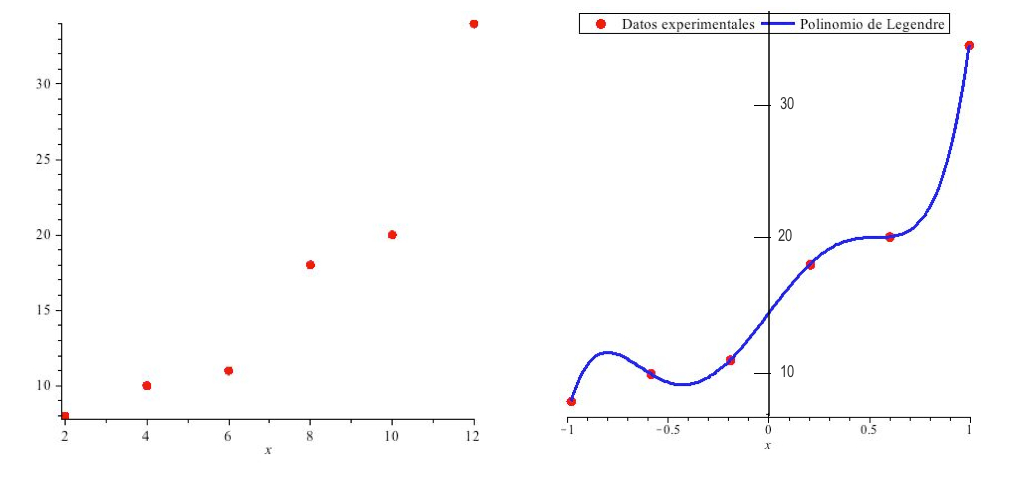
\includegraphics[width=5.8in]{VOLUMEN_1/02_Espacios_Lineales/Figuras/Figura2_1.jpg}
\caption{A la izquierda los puntos experimentales: $\{ (2, 8), (4,10), (6,11), (8,18), (10,20), (12,34) \}$ y a la derecha la funci�n polin�mica que los interpola.}
\label{FigPuntExpInterp}
\end{center}
\end{figure}

\[
\begin{array}{r l}
\left(-1,8\right) \,\, \Rightarrow \,\, & 8=C_{{0}}-C_{{1}}+C_{{2}}-C_{{3}}+C_{{4}}-C_{{5}}     \\ \\
\left(-\frac35,10\right) \,\, \Rightarrow \,\,  &  10=C_{{0}}- \frac{3}{5}\,C_{{1}}+ \frac{1}{25} \,C_{{2}}+{\frac {9}{25}}\,C_{{3}}-{\frac {51}{125}}\,C_{{4}}+{\frac {477}{3125}}\,C_{{5}}    \\ \\
\left(-\frac15,11\right) \,\, \Rightarrow \,\,  & 11=C_{{0}}- \frac{1}{5} \,C_{{1}}-{\frac {11}{25}}\,C_{{2}}+{\frac {7}{25}}\,C_{{3}}+{\frac {29}{125}}\,C_{{4}}-{\frac {961}{3125}}\,C_{{5}}  \\ \\   
\left(\frac15,18\right) \,\, \Rightarrow \,\,  &18=C_{{0}}+ \frac{1}{5} \,C_{{1}}-{\frac {11}{25}}\,C_{{2}}-{\frac {7}{25}}\,C_{{3}}+{\frac {29}{125}}\,C_{{4}}+{\frac {961}{3125}}\,C_{{5}}	\\ \\
\left(\frac35,20\right) \,\, \Rightarrow \,\,  &20=C_{{0}}+ \frac{3}{5}\,C_{{1}}+ \frac{1}{25} \,C_{{2}}-{\frac {9}{25}}\,C_{{3}}-{\frac {51}{125}}\,C_{{4}}-{\frac {477}{3125}}\,C_{{5}}	 \\ \\ 
\left(1,34\right) \,\, \Rightarrow \,\,  & 34=C_{{0}}+C_{{1}}+C_{{2}}+C_{{3}}+C_{{4}}+C_{{5}}
\end{array}
\]

Al resolver este sistema obtendremos:
\[
C_{0} ={\frac {2249}{144}}, \quad C_{1} ={\frac {3043}{336}}, \quad C_{2} ={\frac {1775}{504}},  \quad C_{3} =-{\frac {175}{216}}, \quad C_{4} ={\frac {625}{336}}, \quad C_{5} ={\frac {14375}{3024}}\,,
\] 
con lo cual:
\[
\mathcal{P}(x) = f(x) ={\frac {2249}{144}}+{\frac {3043}{336}}\,x+{\frac {1775}{504}}\,{\it P} \left( 2,x \right) -{\frac {175}{216}}\,{\it P} \left( 3,x \right) +{\frac {625}{336}}\,{\it P} \left( 4,x \right) +{\frac {14375}{3024}}\,
{\it P} \left( 5,x \right)\,.
\] 
y la interpolaci�n queda representada en la figura \ref{FigPuntExpInterp}.

 

N�tese que mientras m�s puntos experimentales se incluyan para la interpolaci�n, el polinomio resultante ser� de mayor grado y, por lo tanto incluir� oscilaciones que distorsionar�n una aproximaci�n m�s razonable. Por ello, la estrategia de hacer la interpolaci�n a trozos, digamos de tres puntos en tres puntos, generar� un mejor ajuste, pero ser� una funci�n (un polinomio) continua a trozos.

\newpage
\subsection{{\color{red}Practicando con Maxima}} 

\subsubsection{Series de Fourier}
\index{Maxima!Series de Fourier}
\index{Series de Fourier}
Existe una librer�a llamada {\bf fourie} en {\bf Maxima} que contiene instrucciones para el c�lculo simb�lico de  series de Fourier de una funci�n $f(x)$ en el intervalo $[-l,l]$: {\bf fourier} $(f, x, l)$.  Tambi�n encontraremos un conjunto de comandos   en el paquete para calcular los coeficientes y para manipular las expresiones resultantes.

%%%%%% INPUT:
\begin{minipage}[t]{8ex}
{\color{red}\bf \begin{verbatim} (%i1) 
\end{verbatim}}
\end{minipage}
\begin{minipage}[t]{\textwidth}{\color{blue}
\begin{verbatim}
load(fourie)$
\end{verbatim}}
\end{minipage}
\newline

En el ejemplo anterior aproximamos la funci�n: 
\[
f(x)=x^2 \,.
\]

Veamos como se trabaja con el programa para calcular la serie de Fourier. Los resultados aparecer�n en la forma de listas temporales y entre ellas los coeficientes. Las listas temporales ser�n indicadas con la notaci�n $(\% {\tt t} \, )$.

%%%%%% INPUT:
\begin{minipage}[t]{8ex}
{\color{red}\bf \begin{verbatim} (%i2) 
\end{verbatim}}
\end{minipage}
\begin{minipage}[t]{\textwidth}{\color{blue}
\begin{verbatim}
f:x^2;
\end{verbatim}}
\end{minipage}

%%% OUTPUT:
\begin{math}\displaystyle \parbox{8ex}{\color{labelcolor}(\%o2) }
x^2
\end{math}

%%%%%% INPUT:
\begin{minipage}[t]{8ex}
{\color{red}\bf \begin{verbatim} (%i3) 
\end{verbatim}}
\end{minipage}
\begin{minipage}[t]{\textwidth}{\color{blue}
\begin{verbatim}
fourier(f,x,%pi);
\end{verbatim}}
\end{minipage}

%%% OUTPUT:
\begin{math}\displaystyle \parbox{8ex}{\color{labelcolor}(\%t3) }
a_{0}={{\pi^2}\over{3}}
\end{math}

%%% OUTPUT:
\begin{math}\displaystyle \parbox{8ex}{\color{labelcolor}(\%t4) }
a_{n}={{2\,\left({{\pi^2\,\sin \left(\pi\,n\right)}\over{n}}-{{2\,
 \sin \left(\pi\,n\right)}\over{n^3}}+{{2\,\pi\,\cos \left(\pi\,n
 \right)}\over{n^2}}\right)}\over{\pi}}
\end{math}

%%% OUTPUT:
\begin{math}\displaystyle \parbox{8ex}{\color{labelcolor}(\%t5) }
b_{n}=0
\end{math}

%%% OUTPUT:
\begin{math}\displaystyle \parbox{8ex}{\color{labelcolor}(\%o5) }
\left[ { \%t_3} , { \%t_4} , { \%t_5} \right] 
\end{math}
\newline

Lo anterior se puede simplificar  con el comando {\bf foursimp}:

%%%%%% INPUT:
\begin{minipage}[t]{8ex}
{\color{red}\bf \begin{verbatim} (%i6) 
\end{verbatim}}
\end{minipage}
\begin{minipage}[t]{\textwidth}{\color{blue}
\begin{verbatim}
foursimp(%);
\end{verbatim}}
\end{minipage}

%%% OUTPUT:
\begin{math}\displaystyle \parbox{8ex}{\color{labelcolor}(\%t6) }
a_{0}={{\pi^2}\over{3}}
\end{math}

%%% OUTPUT:
\begin{math}\displaystyle \parbox{8ex}{\color{labelcolor}(\%t7) }
a_{n}={{4\,\left(-1\right)^{n}}\over{n^2}}
\end{math}

%%% OUTPUT:
\begin{math}\displaystyle \parbox{8ex}{\color{labelcolor}(\%t8) }
b_{n}=0
\end{math}

%%% OUTPUT:
\begin{math}\displaystyle \parbox{8ex}{\color{labelcolor}(\%o8) }
\left[ {\%t_6} , { \%t_7} , { \%t_8} \right] 
\end{math}
\newline

Podemos evaluar la lista de los coeficiente hasta el t�rmino $k$. Aqu� lo haremos hasta $k=4$ y el resultado lo lo asignaremos a la variable $F$. Por otro lado, 
usaremos $(\% {\tt o} 8 )$, la �ltima salida, como entrada para siguiente comando.

%%%%%% INPUT:
\begin{minipage}[t]{8ex}
{\color{red}\bf \begin{verbatim} (%i9) 
\end{verbatim}}
\end{minipage}
\begin{minipage}[t]{\textwidth}{\color{blue}
\begin{verbatim}
F:fourexpand(%o8,x,%pi,4);
\end{verbatim}}
\end{minipage}

%%% OUTPUT:
\begin{math}\displaystyle \parbox{8ex}{\color{labelcolor}(\%o9) }
{{\cos \left(4\,x\right)}\over{4}}-{{4\,\cos \left(3\,x\right)
 }\over{9}}+\cos \left(2\,x\right)-4\,\cos x+{{\pi^2}\over{3}}
\end{math}
\newline 

Construiremos ahora en un mismo gr�fico la funci�n original y los primeros $5$ t�rminos de la serie, de esta manera podremos  comparar el resultado de la aproximaci�n. Las opciones para realizar los diferentes gr�ficos en {\bf Maxima} se pueden consultar en el manual de programa. 

%%%%%% INPUT:
\begin{minipage}[t]{8ex}
{\color{red}\bf \begin{verbatim} (%i10) 
\end{verbatim}}
\end{minipage}
\begin{minipage}[t]{\textwidth}{\color{blue}
\begin{verbatim}
wxplot2d([F,f], [x,-%pi,%pi],[legend, "F", "x^2"])$
\end{verbatim}}
\end{minipage}

%%% OUTPUT:
\begin{math}\displaystyle \parbox{8ex}{\color{labelcolor}(\%o10) }
\end{math}
\begin{figure}[h]\nonumber
\begin{center}
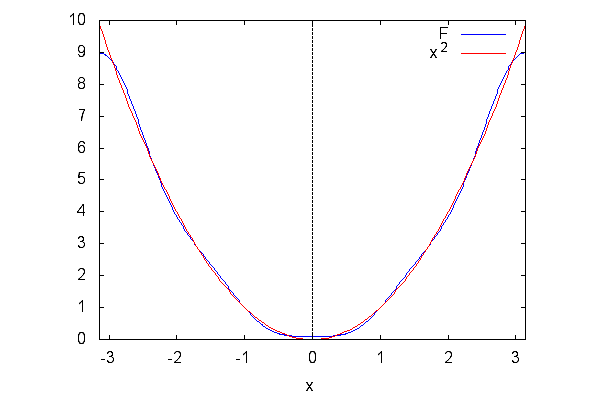
\includegraphics[height=2.6in,width=4.5in]{VOLUMEN_1/02_Espacios_Lineales/Figuras/Figura2_0}
\end{center}
\end{figure}
\newline

Veamos que sucede si escribimos:

%%%%%% INPUT:
\begin{minipage}[t]{8ex}
{\color{red}\bf \begin{verbatim} (%i11) 
\end{verbatim}}
\end{minipage}
\begin{minipage}[t]{\textwidth}{\color{blue}
\begin{verbatim}
totalfourier(f,x,%pi);
\end{verbatim}}
\end{minipage}

%%% OUTPUT:
\begin{math}\displaystyle \parbox{8ex}{\color{labelcolor}(\%t11) }
a_{0}=\frac{\pi^2}{3}
\end{math}

%%% OUTPUT:
\begin{math}\displaystyle \parbox{8ex}{\color{labelcolor}(\%t12) }
a_{n}=\frac{2\,\left(\frac{\pi^2\,\sin \left(\pi\,n\right)}{n}-
 \frac{2\,\sin \left(\pi\,n\right)}{n^3}+\frac{2\,\pi\,\cos \left(\pi
 \,n\right)}{n^2}\right)}{\pi}
\end{math}

%%% OUTPUT:
\begin{math}\displaystyle \parbox{8ex}{\color{labelcolor}(\%t13) }
b_{n}=0
\end{math}

%%% OUTPUT:
\begin{math}\displaystyle \parbox{8ex}{\color{labelcolor}(\%t14) }
a_{0}=\frac{\pi^2}{3}
\end{math}

%%% OUTPUT:
\begin{math}\displaystyle \parbox{8ex}{\color{labelcolor}(\%t15) }
a_{n}=\frac{4\,\left(-1\right)^{n}}{n^2}
\end{math}

%%% OUTPUT:
\begin{math}\displaystyle \parbox{8ex}{\color{labelcolor}(\%t16) }
b_{n}=0
\end{math}

%%% OUTPUT:
\begin{math}\displaystyle \parbox{8ex}{\color{labelcolor}(\%o16) }
4\,\sum_{n=1}^{\infty }{\frac{\left(-1\right)^{n}\,\cos \left(n\,x
 \right)}{n^2}}+\frac{\pi^2}{3}
\end{math}
\newline

En este caso fueron aplicados de manera simult�nea los comandos {\bf fourier} y {\bf foursimp} para finalmente presentar la serie en forma de una sumatoria.  

%%%%%% INPUT:
\begin{minipage}[t]{8ex}
{\color{red}\bf \begin{verbatim} (%i17) 
\end{verbatim}}
\end{minipage}
\begin{minipage}[t]{\textwidth}{\color{blue}
\begin{verbatim}
kill(all)$
\end{verbatim}}
\end{minipage}
%\newpage

\subsubsection{M�nimos Cuadrados}  

{\bf Maxima} puede estimar  los par�metros que mejor se ajusten a una funci�n $f=(x,y)$  para un conjunto de datos, utilizando el m�todo de m�nimos cuadrados. El programa buscar� primero una soluci�n exacta, si no la encuentra buscar� una aproximada. El resultado lo presentar� como una lista de ecuaciones. La funci�n a utilizar ser� {\bf lsquares}. 

Vamos a considerar los ejemplos estudiados con anterioridad:

\begin{enumerate}
\item En el primer ejemplo los datos eran los siguientes:
\[
\left(x,y\right)=  \left(1,2\right),\left(3,2\right)  ,\left(4,5\right),\left(6,6\right)\,.
\] 

Es necesario hacer  uso de la librer�a {\bf lsquares} y los los datos deben introducirse en forma de matriz.

%%%%%% INPUT:
\begin{minipage}[t]{8ex}
{\color{red}\bf \begin{verbatim} (%i1) 
\end{verbatim}}
\end{minipage}
\begin{minipage}[t]{\textwidth}{\color{blue}
\begin{verbatim}
load(lsquares)$ 
\end{verbatim}}
\end{minipage}

%%%%%% INPUT:
\begin{minipage}[t]{8ex}
{\color{red}\bf \begin{verbatim} (%i2) 
\end{verbatim}}
\end{minipage}
\begin{minipage}[t]{\textwidth}{\color{blue}
\begin{verbatim}
datos: matrix([1,2],[3,2],[4,5],[6,6])$
\end{verbatim}}
\end{minipage}
\newline

Por conveniencia, para m�s adelante hacer un gr�fico, convertimos la matrix ``datos'' en una lista. Esto es sencillo si utilizamos el comando {\bf args}:

%%%%%% INPUT:
\begin{minipage}[t]{8ex}
{\color{red}\bf \begin{verbatim} (%i3) 
\end{verbatim}}
\end{minipage}
\begin{minipage}[t]{\textwidth}{\color{blue}
\begin{verbatim}
datosL:args(datos);
\end{verbatim}}
\end{minipage}

%%% OUTPUT:
\begin{math}\displaystyle \parbox{8ex}{\color{labelcolor}(\%o3) }
\left[ \left[ 1 , 2 \right]  , \left[ 3 , 2 \right]  , \left[ 4 , 5
\right]  , \left[ 6 , 6 \right]  \right]
\end{math}
\newline

Supondremos entonces que los puntos se ajustan a un polinomio  lineal del tipo:  $y=ax$. El par�metro $a$  se calcula con la funci�n { \bf lsquares estimates}. Es importante prestar bastante atenci�n a la sintaxis del siguiente comando.
 
%%%%%% INPUT:
\begin{minipage}[t]{8ex}
{\color{red}\bf \begin{verbatim} (%i4) 
\end{verbatim}}
\end{minipage}
\begin{minipage}[t]{\textwidth}{\color{blue}
\begin{verbatim}
param: lsquares_estimates(datos,[x,y],y=a*x,[a]), numer;
\end{verbatim}}
\end{minipage}

%%% OUTPUT:
\begin{math}\displaystyle \parbox{8ex}{\color{labelcolor}(\%o4) }
\left[ \left[ a=1.032258064516129  \right] 
  \right] 
\end{math}
\newline

Este ser� entonces el valor del par�metro $a$ de la ecuaci�n de la recta $y=ax$ que pasa por el origen. Notemos tambi�n que le hemos asignado el valor del par�metro $a$ a la variable ${\tt param}$.

Lo que haremos ahora es escribir la ecuaci�n de dicha recta. Podemos hacer uso de la instrucci�n {\bf ev} que nos permite evaluar una expresi�n. 

%%%%%% INPUT:
\begin{minipage}[t]{8ex}
{\color{red}\bf \begin{verbatim} (%i5) 
\end{verbatim}}
\end{minipage}
\begin{minipage}[t]{\textwidth}{\color{blue}
\begin{verbatim}
y:ev(a*x,first(param));
\end{verbatim}}
\end{minipage}

%%% OUTPUT:
\begin{math}\displaystyle \parbox{8ex}{\color{labelcolor}(\%o5) }
1.032258064516129\,x
\end{math}
\newline

Procederemos ahora a graficar los datos experimentales $vs$ el ajuste por m�nimos cuadrados en un mismo gr�fico. Recordemos que el conjunto de puntos lo tenemos en la forma de una lista, que hemos denominada m�s arriba como ${\tt datosL}$. Mientras que al ajuste que hemos calculado, es decir, la recta: $1.032258064516129\,x$' le hemos asignado la variable denominada $y$. 

Es recomendable consultar el manual del programa, en la parte  que tiene que ver con gr�ficos,  {\bf plot2d},  {\bf plot3d}, para identificar la sintaxis que aparecer� en la siguiente instrucci�n.
%\newpage

%%%%%% INPUT:
\begin{minipage}[h]{8ex}
{\color{red}\bf \begin{verbatim} (%i6) 
\end{verbatim}}
\end{minipage}
\begin{minipage}[h]{\textwidth}{\color{blue}
\begin{verbatim}
wxplot2d([[discrete,datosL], y], [x,0,10],[style, [points,5,2], [lines,2,1]],
[point_type, plus], [legend,"Datos","y=ax"],[xlabel, "x"],[ylabel, "y"])$
\end{verbatim}}

\end{minipage}
%%% OUTPUT:
\begin{math}\displaystyle \parbox{8ex}{\color{labelcolor}(\%o6) }
\end{math}
\begin{figure}[h]\nonumber
\begin{center}
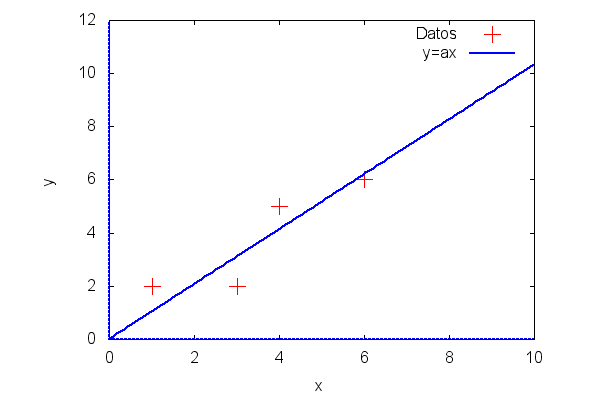
\includegraphics[height=2.5in,width=4.5in]{VOLUMEN_1/02_Espacios_Lineales/Figuras/Figura2_2.jpg}
\end{center}
\end{figure}
\newline

Nota: Se deja como ejercicio repetir �ste mismo  c�lculo pero usando un ajuste para  los datos de la forma: $y=ax+b$.

\item Consideremos el conjunto de datos:
$\left|  {x}_{1}\right> =\left(  1,2,1,1\right)\,,\,\, \left|{x}_{2}\right> =\left(  2,1,1,-1\right) \,,\,\, \left|{y}\right> =\left(  15,12,10,0\right)$. Vamos a suponer que ajustan de la manera siguiente: $\left|{y}\right> = a\left|{x}_{1}\right> + b\left|{x}_{2}\right>$.

%%%%%% INPUT:
\begin{minipage}[t]{8ex}
{\color{red}\bf \begin{verbatim} (%i7) 
\end{verbatim}}
\end{minipage}
\begin{minipage}[t]{\textwidth}{\color{blue}
\begin{verbatim}
datos2: matrix([1,2,15],[2,1,12],[1,1,10],[1,-1,0])$
\end{verbatim}}
\end{minipage}
\newline

Cambiemos ligeramente la notaci�n por: $z=ax+by$ y calculemos los par�metros $a$ y $b$.

%%%%%% INPUT:
\begin{minipage}[t]{8ex}
{\color{red}\bf \begin{verbatim} (%i8) 
\end{verbatim}}
\end{minipage}
\begin{minipage}[t]{\textwidth}{\color{blue}
\begin{verbatim}
param: lsquares_estimates(datos2,[x,y,z], z=a*x+b*y,[a,b]), numer;
\end{verbatim}}
\end{minipage}
%%% OUTPUT:
\begin{math}\displaystyle \parbox{8ex}{\color{labelcolor}(\%o8) }
\left[ \left[ a=4.090909090909091 , b=5.090909090909091 \right] 
\right] 
\end{math}

\item Para el tercer ejemplo se consideraron los siguientes datos:
\[
\left\{  \left(0,1\right), \left(  1,3\right), \left(2,7\right), \left(3,15\right)  \right\}  
\quad\Leftrightarrow\quad y=ax^{2}+bx+c \,.
\]

Haremos con {\bf Maxima} el c�lculo directo usando un ajuste cuadr�tico para los datos suministrados.

%%%%%% INPUT:
\begin{minipage}[t]{8ex}
{\color{red}\bf \begin{verbatim} (%i9) 
\end{verbatim}}
\end{minipage}
\begin{minipage}[t]{\textwidth}{\color{blue}
\begin{verbatim}
datos3: matrix([0,1],[1,3],[2,7],[3,15])$
\end{verbatim}}
\end{minipage}
%%%%%% INPUT:
\begin{minipage}[t]{8ex}
{\color{red}\bf \begin{verbatim} (%i10) 
\end{verbatim}}
\end{minipage}
\begin{minipage}[t]{\textwidth}{\color{blue}
\begin{verbatim}
datosL3: args(datos3)$
\end{verbatim}}
\end{minipage}
%%%%%% INPUT:
\begin{minipage}[t]{8ex}
{\color{red}\bf \begin{verbatim} (%i11) 
\end{verbatim}}
\end{minipage}
\begin{minipage}[t]{\textwidth}{\color{blue}
\begin{verbatim}
param: lsquares_estimates(datos3,[x,y], y=a*x^2+b*x+c,[a,b,c]), numer;
\end{verbatim}}
\end{minipage}
%%% OUTPUT:
\begin{math}\displaystyle \parbox{8ex}{\color{labelcolor}(\%o11) }
\left[ \left[ a=1.5 , b=0.1 , c=1.1 \right]  \right] 
\end{math}

%%%%%% INPUT:
\begin{minipage}[t]{8ex}
{\color{red}\bf \begin{verbatim} (%i12) 
\end{verbatim}}
\end{minipage}
\begin{minipage}[t]{\textwidth}{\color{blue}
\begin{verbatim}
y2:ev(a*x^2+b*x+c,first(param))$
\end{verbatim}}
\end{minipage}
\newline

Como hicimos anteriormente, graficamos los datos y el ajuste cuadr�tico en una misma figura.

%%%%%% INPUT:
\begin{minipage}[t]{8ex}
{\color{red}\bf \begin{verbatim} (%i13) 
\end{verbatim}}
\end{minipage}
\begin{minipage}[t]{\textwidth}{\color{blue}
\begin{verbatim}
wxplot2d([[discrete,datosL3], y2], [x,0,4],[style, [points,5,2], [lines,2,1]],
[point_type, plus], [legend,"Datos","y=ax^2+bx+c"],[xlabel, "x"],[ylabel, "y"])$
\end{verbatim}}
\end{minipage}
%%% OUTPUT:
\begin{math}\displaystyle \parbox{8ex}{\color{labelcolor}(\%o13) }
\end{math}
\begin{figure}[h]\nonumber
\begin{center}
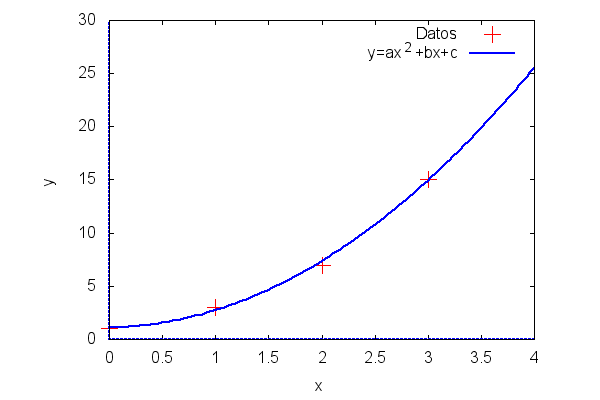
\includegraphics[height=2.6in,width=4.5in]{VOLUMEN_1/02_Espacios_Lineales/Figuras/Figura2_3.jpg}
\end{center}
\end{figure}
\end{enumerate}

%%%%%% INPUT:
\begin{minipage}[t]{8ex}
{\color{red}\bf \begin{verbatim} (%i14) 
\end{verbatim}}
\end{minipage}
\begin{minipage}[t]{\textwidth}{\color{blue}
\begin{verbatim}
kill(all)$
\end{verbatim}}
\end{minipage}

\subsubsection{Polinomios ortogonales}
\index{Maxima!Polinomios ortogonales}
\index{Polinomios ortogonales}
{\bf Maxima} contiene la librer�a {\bf orthopoly} que nos permite acceder a la evaluaci�n simb�lica y num�rica de los diferentes tipos de polinomios ortogonales: Chebyshev, Laguerre, Hermite, Jacobi, Legendre... 

%%%%%% INPUT:
\begin{minipage}[t]{8ex}
{\color{red}\bf \begin{verbatim} (%i1) 
\end{verbatim}}
\end{minipage}
\begin{minipage}[t]{\textwidth}{\color{blue}
\begin{verbatim}
load (orthopoly)$
\end{verbatim}}
\end{minipage}
\newline

Por ejemplo, para obtener los primeros 6 polinomios de Legendre escribimos los siguientes comandos: 

%%%%%% INPUT:
\begin{minipage}[t]{8ex}
{\color{red}\bf \begin{verbatim} (%i2) 
\end{verbatim}}
\end{minipage}
\begin{minipage}[t]{\textwidth}{\color{blue}
\begin{verbatim}
[legendre_p(0,x),legendre_p(1,x),legendre_p(2,x), 
legendre_p(3,x),legendre_p(4,x),legendre_p(5,x)]$
\end{verbatim}}
\end{minipage}
\newline

Simplificamos con {\bf ratsimp}:

%%%%%% INPUT:
\begin{minipage}[t]{8ex}
{\color{red}\bf \begin{verbatim} (%i3) 
\end{verbatim}}
\end{minipage}
\begin{minipage}[t]{\textwidth}{\color{blue}
\begin{verbatim}
ratsimp (%);
\end{verbatim}}
\end{minipage}

%%% OUTPUT:
\begin{math}\displaystyle \parbox{8ex}{\color{labelcolor}(\%o3) }
\left[ 1 , x , \frac{3\,x^2-1}{2} , \frac{5\,x^3-3\,x}{2} , \frac{
 35\,x^4-30\,x^2+3}{8} , \frac{63\,x^5-70\,x^3+15\,x}{8} \right] 
\end{math}
%\newpage

Los diferentes polinomios de Legendre se pueden visualizar de la manera siguiente:

%%%%%% INPUT:
\begin{minipage}[t]{8ex}
{\color{red}\bf \begin{verbatim} (%i4) 
\end{verbatim}}
\end{minipage}
\begin{minipage}[t]{\textwidth}{\color{blue}
\begin{verbatim}
wxplot2d(%,[x,-1,1],[legend, "P0", "P1","P2", "P3","P4", "P5" ])$
\end{verbatim}}
\end{minipage}

%%% OUTPUT:
\begin{math}\displaystyle \parbox{8ex}{\color{labelcolor}(\%o4) }
\end{math}
\begin{figure}[h]\nonumber
\begin{center}
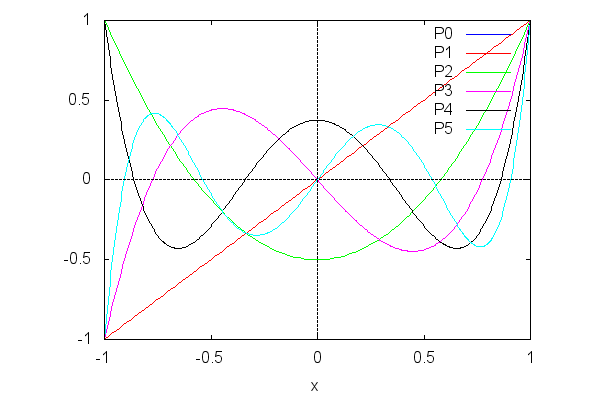
\includegraphics[height=2.6in,width=4.5in]{VOLUMEN_1/02_Espacios_Lineales/Figuras/Figura2_4.jpg}
\end{center}
\end{figure}

Ahora bien, con los datos de la figura \ref{FigPuntExpInterp} se plante� un sistema de ecuaciones lineales:

%%%%%% INPUT:
\begin{minipage}[t]{8ex}
{\color{red}\bf \begin{verbatim} (%i5) 
\end{verbatim}}
\end{minipage}
\begin{minipage}[t]{\textwidth}{\color{blue}
\begin{verbatim}
ecu1:C0-C1+C2-C3+C4-C5=8$
\end{verbatim}}
\end{minipage}

%%%%%% INPUT:
\begin{minipage}[t]{8ex}
{\color{red}\bf \begin{verbatim} (%i6) 
\end{verbatim}}
\end{minipage}
\begin{minipage}[t]{\textwidth}{\color{blue}
\begin{verbatim}
ecu2:C0-3/5*C1+1/25*C2+9/25*C3-51/125*C4+477/3125*C5=10$
\end{verbatim}}
\end{minipage}

%%%%%% INPUT:
\begin{minipage}[t]{8ex}
{\color{red}\bf \begin{verbatim} (%i7) 
\end{verbatim}}
\end{minipage}
\begin{minipage}[t]{\textwidth}{\color{blue}
\begin{verbatim}
ecu3:C0-1/5*C1-11/25*C2+7/25*C3+29/125*C4-961/3125*C5=11$
\end{verbatim}}
\end{minipage}

%%%%%% INPUT:
\begin{minipage}[t]{8ex}
{\color{red}\bf \begin{verbatim} (%i8) 
\end{verbatim}}
\end{minipage}
\begin{minipage}[t]{\textwidth}{\color{blue}
\begin{verbatim}
ecu4:C0+1/5*C1-11/25*C2-7/25*C3+29/125*C4+961/3125*C5=18$
\end{verbatim}}
\end{minipage}

%%%%%% INPUT:
\begin{minipage}[t]{8ex}
{\color{red}\bf \begin{verbatim} (%i9) 
\end{verbatim}}
\end{minipage}
\begin{minipage}[t]{\textwidth}{\color{blue}
\begin{verbatim}
ecu5:C0+3/5*C1+1/25*C2-9/25*C3-51/125*C4-477/3125*C5=20$
\end{verbatim}}
\end{minipage}

%%%%%% INPUT:
\begin{minipage}[t]{8ex}
{\color{red}\bf \begin{verbatim} (%i10) 
\end{verbatim}}
\end{minipage}
\begin{minipage}[t]{\textwidth}{\color{blue}
\begin{verbatim}
ecu6:C0+C1+C2+C3+C4+C5=34$
\end{verbatim}}
\end{minipage} 
\newline

Resolvemos el sistema anterior:

%%%%%% INPUT:
\begin{minipage}[t]{8ex}
{\color{red}\bf \begin{verbatim} (%i11) 
\end{verbatim}}
\end{minipage}
\begin{minipage}[t]{\textwidth}{\color{blue}
\begin{verbatim}
linsolve([ecu1,ecu2,ecu3,ecu4,ecu5,ecu6], [C0,C1,C2,C3,C4,C5]);\end{verbatim}}
\end{minipage} 

%%% OUTPUT:
\begin{math}\displaystyle \parbox{8ex}{\color{labelcolor}(\%o11) }
\left[ {\it C_0}=\frac{2249}{144} , {\it C_1}=\frac{3043}{336} , 
 {\it C_2}=\frac{1775}{504} , {\it C_3}=-\frac{175}{216} , {\it C_4}=
 \frac{625}{336} , {\it C_5}=\frac{14375}{3024} \right] 
\end{math}
\newline

Para asignar cada soluci�n a la variable correspondiente podemos hacer lo siguiente:

%%%%%% INPUT:
\begin{minipage}[t]{8ex}
{\color{red}\bf \begin{verbatim} (%i12) 
\end{verbatim}}
\end{minipage}
\begin{minipage}[t]{\textwidth}{\color{blue}
\begin{verbatim}
[C0,C1,C2,C3,C4,C5]:[rhs(%[1]),rhs(%[2]),rhs(%[3]),rhs(%[4]),rhs(%[5]),rhs(%[6])];
\end{verbatim}}
\end{minipage} 

%%% OUTPUT:
\begin{math}\displaystyle \parbox{8ex}{\color{labelcolor}(\%o12) }
\left[ \frac{2249}{144} , \frac{3043}{336} , \frac{1775}{504} , -
 \frac{175}{216} , \frac{625}{336} , \frac{14375}{3024} \right] \end{math}
%\newpage

Por lo tanto, la funci�n aproximada ser�:

%%%%%% INPUT:
\begin{minipage}[t]{8ex}
{\color{red}\bf \begin{verbatim} (%i13) 
\end{verbatim}}
\end{minipage}
\begin{minipage}[t]{\textwidth}{\color{blue}
\begin{verbatim}
f:C0+C1*legendre_p(1,x)+C2*legendre_p(2,x)+C3*legendre_p(3,x)
+C4*legendre_p(4,x)+legendre_p(5,x)*C5$
\end{verbatim}}
\end{minipage} 

%%%%%% INPUT:
\begin{minipage}[t]{8ex}
{\color{red}\bf \begin{verbatim} (%i14) 
\end{verbatim}}
\end{minipage}
\begin{minipage}[t]{\textwidth}{\color{blue}
\begin{verbatim}
f:expand(%);
\end{verbatim}}
\end{minipage} 

%%% OUTPUT:
\begin{math}\displaystyle \parbox{8ex}{\color{labelcolor}(\%o14) }
\frac{14375\,x^5}{384}+\frac{3125\,x^4}{384}-\frac{8375\,x^3}{192}-
\frac{325\,x^2}{192}+\frac{7367\,x}{384}+\frac{1863}{128}
\end{math}
\newline

Procedemos a introducir los datos:

%%%%%% INPUT:
\begin{minipage}[t]{8ex}
{\color{red}\bf \begin{verbatim} (%i15) 
\end{verbatim}}
\end{minipage}
\begin{minipage}[t]{\textwidth}{\color{blue}
\begin{verbatim}
datos:[[-1,8],[-3/5,10],[-1/5,11],[1/5,18],[3/5,20],[1,34]];
\end{verbatim}}
\end{minipage} 

%%% OUTPUT:
\begin{math}\displaystyle \parbox{8ex}{\color{labelcolor}(\%o15) }
\left[ \left[ -1 , 8 \right]  , \left[ -\frac{3}{5} , 10 \right] 
  , \left[ -\frac{1}{5} , 11 \right]  , \left[ \frac{1}{5} , 18
  \right]  , \left[ \frac{3}{5} , 20 \right]  , \left[ 1 , 34
  \right]  \right] 
\end{math}
\newline

Para finalizar, haremos la gr�fica con los datos y con la interpolaci�n:

%%%%%% INPUT:
\begin{minipage}[t]{8ex}
{\color{red}\bf \begin{verbatim} (%i16) 
\end{verbatim}}
\end{minipage}
\begin{minipage}[t]{\textwidth}{\color{blue}
\begin{verbatim}
wxplot2d([[discrete,datos],f], [x,-1,1],[style, [points,5,2], [lines,2,1]],
[point_type, plus],[legend, false],[xlabel, "x"],[ylabel, "y"])$
\end{verbatim}}
\end{minipage} 

%%% OUTPUT:
\begin{math}\displaystyle \parbox{8ex}{\color{labelcolor}(\%o16) }
\end{math}
\begin{figure}[h]\nonumber
\begin{center}
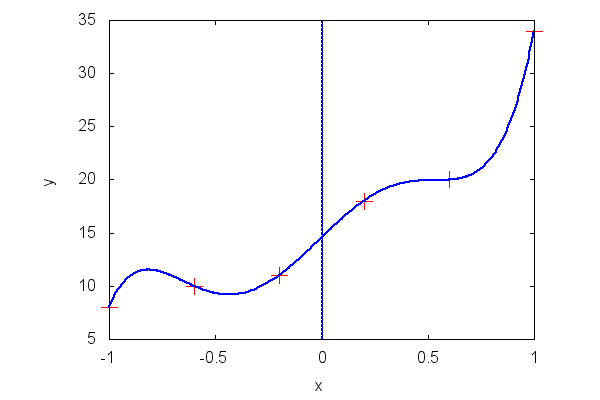
\includegraphics[height=2.6in,width=4.5in]{VOLUMEN_1/02_Espacios_Lineales/Figuras/Figura2_5.jpg}
\end{center}
\end{figure}

\begin{center}
{\color{red}\rule{15.8cm}{0.4mm}}
\end{center}

\subsection{{\color{OliveGreen}Ejercicios}}
\begin{enumerate}
\item 
Demuestre que con las identidades siguientes: 
\[
\cos(kx)= \frac{e^{ikx}+e^{-ikx}}{2} \,,\quad 
\mbox{sen}(kx)= \frac{e^{ikx}-e^{-ikx}}{2i} \,,
\]
la serie de Fourier definida para funciones en el intervalo $(t, t+2\pi)$ se escribe en su forma compleja como:
\[
f\left(x\right) =\frac{1}{2}a_{0}+\sum_{k=1}^{\infty} \left[ a_{k}\cos
(kx)+b_{k}\mathrm{sen}(kx)\right] \,\,\Rightarrow\,\, f \left(x\right) =
\sum_{k=-\infty}^{\infty}  c_k e^{ikx}\,,
\]
con:
\[
c_k=\frac{1}{2\pi}\int_{t}^{t+2\pi} f(x)e^{-{i k x}}\mathrm{d}x\,.
\]

Y que para funciones definidas en el intervalo $(l, l+2L)$ como:
\[
f\left(x\right) =\sum_{k=-\infty}^{\infty}  c_k e^{\frac{i k\pi x}{L}} \,, \quad
\mbox{con} \,\, c_k=\frac{1}{2L}\int_{l}^{l+2L} f(x)e^{-\frac{i k\pi x}{L}}
\mathrm{d}x \,.
\]

Nota: Para los siguientes ejercicios supondremos la utilizaci�n del programa {\bf Maxima}.

\item Para las siguientes funciones determine la serie de Fourier calculando los coeficientes como en la secci�n 
\ref{AproximacionFunciones} y compare los resultados con los c�lculos hechos en el ambiente de manipulaci�n simb�lica. 
\begin{enumerate}
\item $f(x)=x\,�\mbox{sen}(x)  $, si $ -\pi < x < \pi$.
\item $f(x)=e^{x}  $, si $ -\pi < x < \pi$.
\item $f(x)=x  $, si $ 0 < x < 2$.
\item $f(x)=2x-1  $, si $ 0 < x < 1$.
\end{enumerate}
 
\item  Considere el espacio vectorial, $\mathcal{C}^{\infty}_{[-1,1]}$, de funciones reales, continuas y continuamente diferenciables definidas en el intervalo $[-1,1]$. Es claro que una posible base de este espacio de funciones la constituye el conjunto de monomios $\left\{ 1, x, x^{2}, x^{3}, x^{4}, \cdots  \right\}$ por cuanto estas funciones son linealmente independientes. 
\begin{enumerate}
  \item Si suponemos que este espacio vectorial est� equipado con un producto interno definido por $\left< f |g \right> = \int_{-1}^{1}\; \mathrm{d}x \; f(x) g(x) $, muestre que esa base de funciones no es ortogonal.
  
  \item Utilizando la definici�n de producto interno $\left< f |g \right> = \int_{-1}^{1}\; \mathrm{d}x \; f(x) g(x) $ ortogonalize la base $\left\{ 1, x, x^{2}, x^{3}, x^{4}, \cdots  \right\}$ y encuentre los 10 primeros vectores ortogonales, base  para $\mathcal{C}^{\infty}_{[-1,1]}$. Esta nueva base de polinomios ortogonales se conoce como los polinomios de Legendre. 

  \item Modifique un poco la definici�n de producto interno $\left< f |g \right> = \int_{-1}^{1}\; \mathrm{d}x \; f(x) g(x) \sqrt{(1-x^{2})}$ y ortogonalize la base $\left\{ 1, x, x^{2}, x^{3}, x^{4}, \cdots  \right\}$ y encuentre otros 10 primeros vectores ortogonales base para el mismo $\mathcal{C}^{\infty}_{[-1,1]}$. Esta nueva base de polinomios ortogonales se conoce como los polinomios de Chebyshev. 

\item Suponga la funci�n $h(x) = \mathrm{sen}(3x)(1-x^{2})$:
\begin{enumerate}
  \item Expanda la funci�n $h(x)$ en t�rminos de la base de monomios y de polinomios de Legendre, grafique, compare y encuentre el grado de los polinomios en los cuales difieren las expansiones.
 \item Expanda la funci�n $h(x)$ en t�rminos de la base de monomios y de polinomios de Chebyshev, grafique, compare y encuentre el grado de los polinomios en los cuales difieren las expansiones.
 \item Expanda la funci�n $h(x)$ en t�rminos de la base de polinomios de Legendre y de Chebyshev, grafique, compare y encuentre el grado de los polinomios en los cuales difieren las expansiones.
\item Estime en cada caso el error que se comete como funci�n del grado del polinomio (o monomio) de la expansi�n. 
\end{enumerate}
�Qu� puede concluir respecto a la expansi�n en una u otra base?
\end{enumerate}

\item  Parecido al ejercicio anterior, considere el espacio vectorial, $\mathcal{C}^{\infty}_{[0,1]}$, de funciones reales, continuas y continuamente diferenciables definidas en el intervalo $[0,1]$. Es claro que otra posible base de este espacio de funciones la constituye el conjunto de funciones exponenciales $\left\{ 1, \mathrm{e}^{x}, \mathrm{e}^{2x}, \mathrm{e}^{3x}, \mathrm{e}^{4x}, \cdots  \right\}$ por cuanto, al igual que el caso anterior estas funciones tambi�n son linealmente independientes. Adicionalmente, considere aqu� la funci�n $g(x) = \cos(3x^{3})(1-x^{2})$, 
\begin{enumerate}
\item Suponga que este espacio vectorial est� equipado con un producto interno definido por $\left< f |g \right> = \int_{0}^{1}\; \mathrm{d}x \; f(x) g(x) $, y muestre que esa base de funciones $\left\{ 1, \mathrm{e}^{x}, \mathrm{e}^{2x}, \mathrm{e}^{3x}, \mathrm{e}^{4x}, \cdots  \right\}$ no es ortogonal.

  \item Utilizando la definici�n de producto interno ortogonalize la base $\left\{ 1, \mathrm{e}^{x}, \mathrm{e}^{2x}, \mathrm{e}^{3x}, \mathrm{e}^{4x}, \cdots  \right\}$ y encuentre los 7 primeros vectores ortogonales, base  para $\mathcal{C}^{\infty}_{[0,1]}$, i.e. $\left\{ 1, E_{1}(x), E_{2}(x), E_{3}(x), E_{4}(x), \cdots  \right\}$. 

\item Encuentre el valor de los coeficientes, $C_{i}$ de la expansi�n  $g_{M}(x) \approx \sum_{i=0}^{7} C_{i} x^{i} $ utilizando la definici�n de producto interno anterior y estime tambi�n el error $\epsilon_M$ en esta aproximaci�n $g_{M}(x) = \sum_{i=0}^{7} C_{i} x^{i} +\epsilon_M$. 
\item Expanda en serie de Taylor la funci�n anterior $g_{T}(x) \approx \sum_{n=0}^{7} \left.\frac{\mathrm{d} g(x)}{\mathrm{d} x}\right|_{x = 0}  \frac{x^{n}}{n!} $, estime el error $\epsilon_T$ y comp�relo con el caso anterior.
\item Ahora encuentre el valor de los coeficientes, $\tilde{C}_{i}$ de la expansi�n  $g_{E}(x) \approx \sum_{m=0}^{7} \tilde{C}_{m} \mathrm{e}^{mx} $ utilizando la definici�n de producto interno anterior y, del mismo modo, estime tambi�n el error $\epsilon_E$ en esta aproximaci�n $g_{E}(x) = \sum_{m=0}^{7} \tilde{C}_{m} \mathrm{e}^{mx}  +\epsilon_E$. ?` Qu� puede concluir de la comparaci�n de los errores $\epsilon_M$, $\epsilon_T$ y $\epsilon_E$ ?
\item A continuaci�n encuentre el valor de los coeficientes, $\bar{C}_{i}$ de la expansi�n  $g_{Eo}(x) \approx \sum_{m=0}^{7} \bar{C}_{m} E_{m}(x) $ y estime tambi�n el error $\epsilon_{Eo}$ en esta aproximaci�n $g_{Eo}(x) = \sum_{m=0}^{7} \bar{C}_{m} E_{m}(x)  +\epsilon_{Eo}$. ?` Otra vez, qu� puede concluir de la comparaci�n de los errores $\epsilon_M$, $\epsilon_T$, $\epsilon_E$ y $\epsilon_{Eo}$?
\item Grafique las funciones $g(x)$, $g_M(x)$, $g_T(x)$, $g_E(x)$ y $g_{Eo}(x)$ y compare con los errores.
\end{enumerate}
\item Al medir la temperatura a lo largo de una barra material obtenemos los
siguientes valores:
\begin{center}
\begin{tabular}
[c]{|l|rrrrrrrrr|} \hline\hline
$x_{i}\,(cm)$ & $1,0$ & $2,0$ & $3,0$ & $4,0$ & $5,0$ & $6,0$ & $7,0$ &
$8,0$ & $9,0$  \\ \hline
$T_{i}\,(^{\circ}C)$ & $14,6$ & $18,5$ & $36,6$ & $30,8$ & $59,2$ & $60,1$
& $62,2$ & $79,4$ & $99,9$ \\ \hline \hline
\end{tabular}
\end{center}

Encuentre, mediante el m�todo de los m�nimos cuadrados los coeficientes que mejor ajustan a la recta $T=ax+b$.


\item Los precios de un determinado producto var�an como se muestra a continuaci�n:
\begin{center}
\begin{tabular}
[c]{|l|rrrrrrrr|} \hline\hline
A�o & $2007$ & $2008$ & $2009$ & $2010$ & $2011$ & $2012$ & $2013$ & $2014$   \\ \hline
Precio & $133.5$ & $132.2$ & $138.7$ & $141.5 $ & $144.2$ & $144.5$
& $148.6$ & $153.8$  \\ \hline \hline
\end{tabular}
\end{center}
Realice una interpolaci�n polinomial que permita modelar estos datos.

\end{enumerate}




\begin{thebibliography}{9}
\bibitem{ArfkenWeberWeber2000}  Arfken, G. B.,Weber, H., Weber, H.J. (2000) \textbf{Mathematical Methods for Physicists} 5ta Edici�n (Academic Press, Nueva York)

\bibitem{BorisenkoTarapov1968}  Scharnhorst, K. (2009) \textbf{Angles in complex vector spaces} Acta Applicandae Mathematica), {\bf 69}(1), 95-103

\bibitem{DennerykKrzywicki1995}  Dennery, P. y Krzywicki, A. (1995) \textbf{Mathematics for Physicists} (Dover Publications Inc, Nueva York)

\bibitem{Harper1971}  Harper, C. (1971) \textbf{Introduction to Mathematical Physics} (\textit{Prentice Hall, Englewood Cliff, N.J:})

\bibitem{Hassani1991}  Hassani, S. (1991) \textbf{Foundations of Mathematical Physics} (\textit{Prentice Hall, International Edition, London:}

\bibitem{RileyHobsonBence2002}  Riley, K.F., Hobson, M.P. y Bence, S.J. (2002) \textbf{Mathematical Methods for Physics and Engineering } (\textit{Cambridge University Press})


\end{thebibliography}


\chapter{Vectores duales y tensores}
\label{CapVectoresDualesTensores}

\section*{La ruta de este cap�tulo}
Este cap�tulo completa el esfuerzo de formalizaci�n de conceptos que comenzamos en el cap�tulo anterior. Iniciamos con el estudio de los funcionales lineales, extendiendo el concepto de funci�n al de una aplicaci�n entre elementos de espacios  vectoriales, lo cual nos llevar� a la definici�n de los espacios vectoriales duales. Incorporamos el concepto de $1-$forma como ese conjunto de funcionales que forman al espacio vectorial dual. Ahora el producto interno se definir� entre $1-$formas y vectores. En la secci�n \ref{Tensores} definiremos una nueva clase de objetos matem�ticos, los tensores, los cuales pueden verse como arreglos multilineales y constituyen una extensi�n de objetos ya conocidos: los escalares, los vectores y las $1-$formas.  Desarrollaremos el �lgebra tensorial y sus leyes de transformaci�n. Ejemplificamos la utilizaci�n de este concepto en F�sica cuando discutimos, en la secci�n \ref{unpardetensores}, el tensor de inercia y el de esfuerzos (\textit{strees}).  En la secci�n \ref{Pseudoeuclidianos} incursionaremos en los espacios pseudoeuclidianos para mostrar una situaci�n en la cual podemos diferenciar $1-$formas de vectores, aprovechamos adem�s para introducir algunas nociones b�sicas de la teor�a especial de la relatividad. Para finalizar, el la secci�n \ref{espaciosdefunciones} extenderemos los conceptos de espacios vectoriales y bases discretas a espacios de funciones y bases continuas y en ese contexto discutimos algunos rudimentos de teor�as de distribuciones. 

\section{Funcionales lineales}
\label{FuncionalesLineales}
\index{Funcionales lineales}
En los cursos m�s elementales de c�lculo se estudiaron funciones de una y m�s variables reales. Estas funciones pueden considerarse que act�an sobre vectores en $\mathds{R}^3$ y podemos extender esta idea para  otras que tengan como argumento vectores de un espacio vectorial abstracto. Comenzaremos con las m�s sencillas, las lineales, que tambi�n son conocidas como {\it operadores lineales}.

Definiremos funcionales lineales  como aquella operaci�n que asocia un n�mero complejo (o real) $\in \textbf{\em K}$ a un vector $\left|  {v}\right> \in\textbf{\em V}$, es decir:
\[
\forall\,\, \left|v\right> \in \textbf{\em V} \quad \Rightarrow 
\mathcal{F}\left[ \left|  {v}\right> \right] \in\mathds{C}\,,
\]
y cumple con:
\[
\mathcal{F}\left[  \alpha\ \left|  {v}_{{1}}\right> +\beta\ \left|  {v}_{2}\right> \right]  \equiv 
\alpha \ \mathcal{F}\left[  \left|  {v}_{{1}}\right> \right] +\beta\ \mathcal{F}\left[  \left|  {v}_{2}\right> \right]\,,
\,\,\forall \,\, \left| {v}_{{1}}\right> ,\left|  {v}_{2}\right> \in \textbf{\em V}\,\, \mbox{y} \,\, \forall \,\, \alpha, \beta \in \textbf{\em K}\,.
\]

En otras palabras, un funcional lineal (o forma lineal) es un {\it morfismo}\footnote{Entenderemos por morfismo a toda regla o mapa que asigne a todo vector $\left|{v}\right>$  de un espacio vectorial $\textbf{\em V}$ un vector $\left|{w}\right>$ de un espacio vectorial $\textbf{\em W}$ y usualmente se denota por $\mathcal{F}: \textbf{\em V} \Rightarrow  \textbf{\em W}$.} del espacio lineal $ \textbf{\em V}$ a un espacio unidimensional $\textbf{\em K}$.

Notemos que cuando se escoge una base $\{\left|\mathrm{e}_i\right>\}$ de un espacio vectorial $\textbf{\em V}$ de manera que para cualquier vector $ \left|v \right> \in \textbf{\em V}$ se especifican sus componentes $\{\xi^1\}$ respecto a esa base, es decir, $\left|v \right>=\xi^i \left|\mathrm{e}_i\right>$, entonces lo que se tiene para cada componente es un funcional lineal, como por ejemplo,  $\mathcal{F}\left[ \left|  {v}\right> \right] =\xi^1$. Algo parecido ocurre con el producto interno, cuando en un espacio vectorial $\textbf{\em V}$ se define el producto escalar 
$\left< v\right.  \left| v_0\right>$, del vector $\left| v\right>$ con un vector fijo $\left| v_0 \right>$, lo que tenemos es un funcional lineal $\mathcal{F}\left[ \left|  {v}\right> \right] =\left< v\right.  \left| v_0\right>= \alpha \in \textbf{\em K}$.

Otro ejemplo sencillo de un funcional lineal es la integral de Riemann que podemos interpretar de la manera siguiente:
\[
\mathcal{I}\left[ \left| f \right>\right]=\int_a^b f_0(x) f(x) \mathrm{d}x \,,
\]
donde $f(x), f_0(x) \in \mathcal{C}_{[a,b]}$, es decir, pertenece al espacio vectorial de funciones reales y continuas en el intervalo $[a,b]$ y $f_0(x)$ es una funci�n que se toma como fija.

\subsection{Espacio vectorial dual}
\label{EspacioVectorialDual}
\index{Dual!Espacios Vectoriales}
\index{Espacios vectoriales duales}
El conjunto de funcionales lineales $\left\{\mathcal{F}_{1},\mathcal{F}_{2},\mathcal{F}_{3}, \cdots,\mathcal{F}_{n},\cdots\right\}$  constituyen a su vez un espacio vectorial, el cual se denomina espacio vectorial dual de $\textbf{\em V}$ --que es el espacio directo-- y se denotar� como $\textbf{\em V}^{\star}$ (aqu� $^{\star}$ no es complejo conjugado). Si $\textbf{\em V}$ es de dimensi�n finita $n$, entonces dim$\textbf{\em V}=$ dim$\textbf{\em V}^{\star}=n$.

Es f�cil convencerse que los funcionales lineales forman un espacio vectorial ya que, dados $\ \mathcal{F}_{1},\mathcal{F}_{2} \in\textbf{\em V}^{\star}$ se tiene:
\[
\left.
\begin{array}
[c]{c}
\left(\mathcal{F}_{1}+\mathcal{F}_{2}\right)\left[ \left|  {v}\right> \right] =
\mathcal{F}_{1}\left[  \left|  {v}\right>\right]+\mathcal{F}_{2}\left[\left|{v}\right> \right] \\
\\
\left(  \alpha\ \mathcal{F}\right)  \left[  \left|  {v}\right>\right]  =
\alpha\ \mathcal{F}\left[  \left|  {v}\right>\right]
\end{array}
\right\}  \quad \forall  \quad \left|  {v}\right> \in \textbf{\em V} \,.
\]
A este espacio lineal se le llama espacio de formas lineales y, a los funcionales se les denomina $1-$formas o covectores.
\index{Covector}

Como ya lo mencionamos, en aquellos espacios lineales con producto interno definido, el mismo producto interno constituye la expresi�n natural del funcional. As� tendremos que:
\[
 \mathcal{F}_{{a}}  \left[  \left|  {v}\right> \right]  \equiv\left< a\right.  \left| {v}\right> \quad\forall{\quad}\left|  {v}
\right> \in\textbf{\em V}\quad\wedge\quad\forall{\quad}\left< a\right|  \in\textbf{\em V}^{\star} \,.
\]

Es claro comprobar que el producto interno garantiza que los $\left\{ \mathcal{F}_{{a}},\mathcal{F}_{{b}},\cdots\right\}$ forman un espacio vectorial:
\[
\left.
\begin{array}
[c]{c}
\left(  \mathcal{F}_{{a}}+\mathcal{F}_{{b}}\right)  \left[\left|  {v}\right> \right]  =
\mathcal{F}_{{a}}\left[\left|  {v}\right> \right]  +\mathcal{F}_{{b}}\left[ \left|  {v}\right> \right]  =\left< {a}\right.
\left|  {v}\right> +\left< {b}\right.  \left| {v}\right> \\
\\
\left(  \alpha\ \mathcal{F}_{{a}}\right)  \left[  \left| {v}\right> \right]  =\left< \alpha{a}\right.
\left|  {v}\right> =\alpha^{\ast}\left< {a}\right. \left|  {v}\right> =\alpha^{\ast}\ \mathcal{F}_{a}\left[  \left|  {v}\right> \right]
\end{array}
\right\}  \quad\forall{\quad}\left|  {v}\right> \in \textbf{\em V} \,.
\]
Esta �ltima propiedad se conoce como antilinealidad. 

Se establece entonces una correspondencia $1$ a $1$ entre \textit{kets} y \textit{bras}, entre vectores y funcionales lineales (o formas diferenciales): 
\[
\lambda_{1}\left|  {v}_{1}\right> +\lambda_{2}\left| {v}_{2}\right> \qquad\rightleftarrows\qquad\lambda_{1}^{\ast}\left< {v}_{1}\right|  +\lambda_{2}^{\ast}\left<{v}_{2}\right| \,,
\]
que ahora podemos precisar de la siguiente forma:
\begin{align*}
\left< {a}\right.  \left|  {v}\right>  & =\left< {v}\right.  \left|  {a}\right> ^{\ast} \,,\\
\left< {a}\right.  \left|  \lambda_{1}{v}_{1}+\lambda_{2}{v}_{2}\right>  &  =\lambda_{1}\left< {a}\right.  \left|  {v}_{1}\right> +\lambda_{2}\left<{a}\right.  \left|  {v}_{2}\right> \,,\\
\left< \lambda_{1}{a}_{1}{+}\lambda_{2}{a}_{2}\right.  \left|  {v}\right>  &  =\lambda_{1}^{\ast}\left< {a}_{1}\right.  \left|  {v}\right>+\lambda_{2}^{\ast}\left< {a}_{2}\right.  \left|  {v}\right>\,.
\end{align*}

M�s a�n, dada una base  $\left\{  \left|  {e}_{1}\right> , \left|  \mathrm{e}_{2}\right> , \cdots \left|  \mathrm{e}_{n}\right> \right\}  $ para $\textbf{\em V}$ siempre es posible asociar una base para $\textbf{\em V}^{\star}$ de tal manera que:
\[
\left|  {v}\right> =
\xi^{i}\left|\mathrm{e}_{i}\right> \,\,\rightleftarrows \,\, \left< {v}\right| = 
\xi_{i}^{\ast}\left< {e}^{i}\right|\,,  \quad\text{con }\,\,
\xi^{i}=\left< {e}^{i}\right.  \left|  {v}\right> \,\, \wedge \,\, 
\xi_{i}^{\ast}=\left< {v}\right.  \left|  \mathrm{e}_{i}\right>,  \quad \text{para } i=1,2,\cdots,n \, .
\]

En un lenguaje arcaico (y muchos textos de mec�nica todav�a lo reproducen) se denota a la base del espacio dual $\left\{ \left< {e}^{i}\right|  \right\}$ como la base rec�proca de la base $\left\{ \left|  \mathrm{e}_{i}\right>  \right\}$, este caso lo ilustraremos m�s adelante. 

Se puede ver tambi�n que si  $\left|  {v}\right>= \xi^i \left|  \mathrm{e}_{i}\right>$, entonces 
\[
\mathcal{F}\left[  \left|  {v}\right> \right] =
\mathcal{F}\left[ \xi^i \left|  \mathrm{e}_{i}\right> \right] =
\xi^{i}\mathcal{F}\left[ \left|  \mathrm{e}_{i}\right> \right]=
\xi^{i}\omega_i \,, \quad \mbox{con } \,\, \mathcal{F}\left[ \left|\mathrm{e}_{i}\right> \right]\equiv \omega_i \,.
\] 

N�tese que estamos utilizando la notaci�n de Einstein en la que �ndices repetidos indican suma. N�tese tambi�n que las bases del espacio dual de formas diferenciales $\left\{\left< {\mathrm{e}}^{k}\right| \right\}$ llevan los �ndices arriba, los llamaremos �ndices  contravariantes, mientras que los �ndices abajo, ser�n covariantes. Por lo tanto, las componentes de las formas diferenciales en una base dada, llevan �ndices abajo $\left< a\right|=a_{i}\left< {\mathrm{e}}^{i}\right|$ mientras que las
componentes de los vectores los llevan arriba $\left|  v\right> = \xi^{j}\left|  {\mathrm{e}}_{j}\right>$.  

Observe tambi�n que dada una base en el espacio directo $\left\{\left|  {\mathrm{e}}_{i}\right>\right\}$ existe una �nica base can�nica en el dual definida como:
\[
\left< \mathrm{e}^{i}\right.\left|\mathrm{e}_{j}\right>=
\mathcal{F}^i\left[ \left|  \mathrm{e}_{j}\right> \right]= \delta^i_j \, .
\]
Esta $1-$forma al actuar sobre un vector arbitrario resulta en:
\[
\mathcal{F}^i\left[ \left| v \right> \right]= 
\mathcal{F}^i\left[ \xi^j\left|  \mathrm{e}_{j} \right> \right]=
\xi^{j}\mathcal{F}^i\left[ \left|  \mathrm{e}_{j}\right> \right]=
\xi^{j}\delta^i_j=\xi^{i} 
\]
su componente contravariante. El conjunto de $1-$formas  $\{ \mathcal{F}^i \}$ ser� linealmente independientes. 

Si $\left| v \right>=\xi^i \left| \mathrm{e}_{i} \right>$ es un vector arbitrario en el espacio directo y 
$\left< a\right|= a_{i}\left< {\mathrm{e}}^{i}\right|$ un vector en
el espacio dual, entonces:
\[
\left< a \right.\left| v \right>= 
\left< a_i \left< {\mathrm{e}}^{i}\right| \right. \left. \xi^j \left| \mathrm{e}_{j} \right> \right> = 
a_i^* \xi^j \left< {\mathrm{e}}^{i} \right.\left| \mathrm{e}_{j} \right>=
a_i^* \xi^j \delta_j^i = a_i^* \xi^i \, ,
\]
y para bases arbitrarias, no ortogonales, $\{ \left|  {\mathrm{w}}_{i}\right> \}$ de  
$\textbf{\em V}$ y $\{\left< {\mathrm{w}}^{i}\right|\}$ de $\textbf{\em V}^{\star}$ se tiene:
$\left< a \right.\left| v \right>= \left< {\mathrm{w}}^{i} \right.\left| \mathrm{w}_{j} \right> a_i^* \xi^j   \, .$


\subsection{Espacios duales y bases rec�procas}
\label{BasesReciprocas}
Un ejemplo que ilustra las bases duales es la construcci�n de las llamadas bases rec�procas que mencionamos anteriormente en los ejercicios de Aplicaciones del �lgebra vectorial en la p�gina \pageref{EjerciciosAplicacionVectores}. Este ejemplo ilustra la pregunta de siempre: si los vectores se representan geom�tricamente como un segmento orientado, con m�dulo, direcci�n y sentido, como representamos geom�tricamente una forma lineal o covector. Los cristal�grafos lograron ejemplificar las bases duales y luego la aplicaci�n de la difracci�n de rayos x a la cristalograf�a potenci� utilidad de este concepto.

\subsubsection{Bases rec�procas}
\label{BaseReciproca}
\index{Rec�procas!Bases de vectores}
\index{Bases rec�procas de vectores}
Consideremos el problema de expandir un vector $\left| a\right>$  con respecto a una base oblicua (no es ortogonal), $\{\left| \mathrm{w}_{i}\right>\}$, de tal forma que, $\left| a\right>= a^i \left| \mathrm{w}_{i}\right>$.
Por simplicidad, tomemos el caso $\mathds{R}^3$, de manera que  $ \mathbf{a} = a^i {\mathrm{\bf w}}_i $ ($i=1,2,3$).   

Al proyectar el vector $\mathbf{a}$ sobre los ejes de alg�n sistema de coordenadas, es posible resolver el sistema de tres ecuaciones que resulta para las inc�gnitas $a^i$. Las bases de vectores $ {\mathrm{\bf w}}_i$ y de formas o covectores $ {\mathrm{\bf w}}^i$ ser�n duales, y por contrucci�n satisfacen ${\mathrm{\bf w}}_i \cdot {\mathrm{\bf w}}^j=\delta^j_i$. Es decir, cada uno de los vectores bases duales es perpendicular a los otros dos de la base dual: ${\mathrm{\bf w}}^1$ ser� perpendicular a ${\mathrm{\bf w}}_2$  y ${\mathrm{\bf w}}_3$: ${\mathrm{\bf w}}^1= \alpha ({\mathrm{\bf w}}_2 \times {\mathrm{\bf w}}_3)$.  Como ${\mathrm{\bf w}}_1 \cdot {\mathrm{\bf w}}^1=1$, entonces:
\[
\alpha {\mathrm{\bf w}}_1 \cdot ({\mathrm{\bf w}}_2 \times {\mathrm{\bf w}}_3)=1 \,\, \Rightarrow  \,\, 
\alpha = \frac{1}{{\mathrm{\bf w}}_1 \cdot ({\mathrm{\bf w}}_2 \times {\mathrm{\bf w}}_3)} 
\,\, \Rightarrow \,\,
{\mathrm{\bf w}}^1= \frac{{\mathrm{\bf w}}_2 \times {\mathrm{\bf w}}_3}{ {\mathrm{\bf w}}_1 \cdot ({\mathrm{\bf w}}_2 \times {\mathrm{\bf w}}_3)}\,,
\]
y en general, es f�cil ver que:
\begin{equation}
{\mathrm{\bf w}}^i= \frac{{\mathrm{\bf w}}_j \times {\mathrm{\bf w}}_k}{{\mathrm{\bf w}}_i \cdot ({\mathrm{\bf w}}_j \times {\mathrm{\bf w}}_k)}\,,
\label{BaseReciproca}
\end{equation}
donde $i,j,k$ son permutaciones c�clicas de $1,2,3$. La definici�n (\ref{BaseReciproca}) nos permite construir la base de 1-formas o covectores, a partir de su ortogonalidad con los vectores de la base directa.  Notemos tambi�n que $V={\mathrm{\bf w}}_i \cdot ({\mathrm{\bf w}}_j \times {\mathrm{\bf w}}_k)$ es el volumen del paralelep�pedo que soportan los vectores $\{ {\mathrm{\bf w}}_i \}$ y que adem�s se puede obtener una expresi�n an�loga para los $\{ {\mathrm{\bf w}}_i \}$ en t�rmino de los $\{{\mathrm{\bf w}}^i \}$. 

Al ser $\{ {\mathrm{\bf w}}_i\}$ y $\{ {\mathrm{\bf w}}^i\}$ duales, 
$
\mathbf{a} = a^j{\mathrm{\bf w}}_j \, \Rightarrow  \,  
{\mathrm{\bf w}}^i \cdot  \mathbf{a}  = {\mathrm{\bf w}}^i \cdot  (a^j {\mathrm{\bf w}}_j) =  a^j ( {\mathrm{\bf w}}^i \cdot {\mathrm{\bf w}}_j)= a^j \delta_j^i =a^i$, con $ i=1,2,3 \,$ 
y equivalentemente, el covector de $\mathbf{a}$: 
$\mathbf{\bar{a}} = \bar{a}_j \mathrm{\bf w}^j \,\, \Rightarrow   \,\,
\mathbf{\bar{a}} \cdot {\mathrm{\bf w}}_i =(\bar{a}_j \mathrm{\bf w}^j) \cdot  \mathrm{\bf w}_i =  \bar{a}_j ( \mathrm{\bf w}^j \cdot  \mathrm{\bf w}_i) =\bar{a}_j \delta_i^j= \bar{a}_i$,  con  $i=1,2,3$. 
Hemos querido enfatizar el car�cter dual del covector $\mathbf{\bar{a}}$ al vector $\mathbf{a}$ y obviamente $\mathbf{\bar{a}} \cdot \mathbf{a} = |\mathbf{a}|^2$.

De la misma ecuaci�n (\ref{BaseReciproca}) se puede ver que la representaci�n gr�fica de una forma ser� una superficie orientada. La figura \ref{IndicesMiller} muestra como, a partir de una base directa de vectores obl�cuos se construyen planos perpendiculares a esos vectores y la orientaci�n (direcci�n y sentido) representan las direcciones de los vectores duales. En cristalograf�a esa base dual se le representa como los �ndices de Miller. 

Claramente si las base directa es ortonormal su dual tambi�n lo ser� y, m�s importante a�n, ambas bases coinciden ${\mathrm{\bf e}}^i \equiv {\mathrm{\bf e}}_i $, y si la base original o directa es dextr�gira su dual tambi�n lo ser�. 

\begin{figure}
\begin{center}
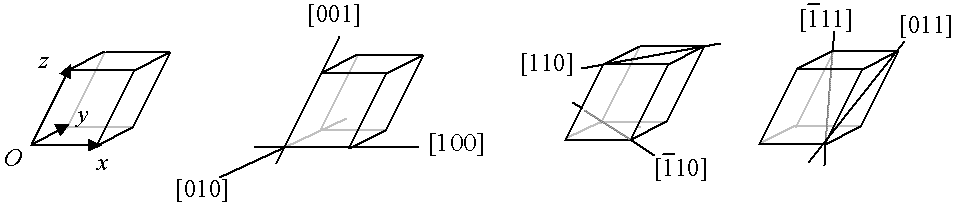
\includegraphics[width=4in]{VOLUMEN_1/03_Funciones_Lineales/Figuras/Indices_miller_direction_exemples}
\caption{Bases directas y rec�procas. Note como los covectores representan planos perpendiculares a dos vectores de la base directa. Figura tomada de \url{https://commons.wikimedia.org/w/index.php?curid=457850} CC BY-SA 3.0,}
\label{IndicesMiller}
\end{center}
\end{figure}

\subsection{Vectores, formas y leyes de transformaci�n}
\label{VectoresLeyesTransformacion}
\index{Leyes de Transformaci�n para vectores}
\index{Vectores!Leyes de Transformaci\'on}
\index{Covectores}

Tal y como hemos mencionado anteriormente (tempranamente en la secci�n \ref{RotacionCoordenadas} y luego en la secci�n \ref{OrtogonalidadBases}),  un determinado vector $\left|  a\right> \in \textbf{\em V}$ puede expresarse en una base ortonormal $\left\{  \left| \mathrm{e}_{j}\right> \right\}$ como: $a^{j}\left| \mathrm{e}_{j}\right> $ donde las $a^{j}$ son las componentes  \textit{contravariantes} del vector en esa base. En general, como es muy largo decir ``componentes del vector contravariante'' uno se refiere (y nos referiremos de ahora en adelante) al conjunto $\left\{  a^{j}\right\}  $ como un \textit{vector contravariante} obviando la precisi�n de \textit{componente}, pero realmente las $a^{j}$ \textbf{son} las componentes del vector.

Adicionalmente, en esta etapa pensaremos a las bases como distintos observadores o sistemas de referencias. Con ello tendremos (algo que ya sab�amos) que un vector se puede expresar en distintas bases y tendr� distintas componentes referidas a esa base
\[
\left|  a\right> =a^{j}\left| \mathrm{e}_{j}\right>
=\tilde{a}^{j}\left|  {\mathrm{\tilde{e}}}_{j}\right> \,.
\]
As� una misma cantidad f�sica vectorial se ver� distinta (tendr� distintas componentes) desde diferentes sistemas de coordenadas.
Las distintas ``visiones'' est�n conectadas mediante un transformaci�n de sistema de referencia como veremos m�s adelante.

Igualmente hemos dicho al comienzo de este cap�tulo (secci�n \ref{EspacioVectorialDual}) que una forma diferencial o 1-forma, $\left< b\right|  \in \textbf{\em V}^{\star}$ es susceptible de expresarse en una base $\left\{  \left< \mathrm{e}^{i}\right|  \right\}$ del espacio dual $\textbf{\em V}^{\star}$ como $b_{i}\left< \mathrm{e}^{i}\right|$ y, como el espacio est� equipado con un producto interno, entonces: 
\[
\left< a\right.  \left|  b\right> =\left< b\right.  \left|a\right> =
b_{i}a^{j}\ \left< \mathrm{e}^{i}\right.  \left|  \mathrm{e}_{j}\right>   = b_{i}a^{j}\delta_{j}^{i}=a^{i}b_{i} \,.
\]
Con lo cual avanzamos otra vez en la interpretaci�n de este tipo de objetos: una cantidad f�sica escalar se ver� igual (ser� invariante) desde  distintos sistemas de referencia.

Adem�s sabemos que unas y otras componentes se relacionan como:
\[
\left.
\begin{array}
[c]{c}
\left< {\mathrm{e}}^{i}\right.  \left|  a\right> =a^{j}\left< {\mathrm{e}}^{i}\right.  \left|  \mathrm{e}_{j}\right> =
a^{j}\delta_{j}^{i}= \tilde{a}^{j}\left< {\mathrm{e}}^{i}\right.  \left| {\mathrm{\tilde{e}}}_{j}\right> \\
\\
\left< {\mathrm{\tilde{e}}}^{i}\right.  \left|  a\right> =
\tilde{a}^{j}\left< {\mathrm{\tilde{e}}}^{i}\right.  \left|  {\mathrm{\tilde{e}}}_{j}\right> =
\tilde{a}^{j}\delta_{j}^{i}=a^{j}\left<{\mathrm{\tilde{e}}}^{i}\right.  \left|  \mathrm{e}_{j}\right>
\end{array}
\right\} \,\, \Rightarrow \,\,
\left\{
\begin{array}
[c]{c}
a^{i}=A_{j}^{i}\tilde{a}^{j}\\ \\
\tilde{a}^{i}=\tilde{A}_{j}^{i}a^{j} \,,
\end{array}
\right.
\]
donde claramente:
\[
\left< {\mathrm{e}}^{i}\right.  \left|  {\mathrm{\tilde{e}}}_{j} \right> = A_{j}^{i};\qquad\left< {\mathrm{\tilde{e}}}^{i}\right. \left|  \mathrm{e}_{j}\right> =
\tilde{A}_{j}^{i} \qquad\text{y} \quad  A_{k}^{i}\tilde{A}_{j}^{k}=
\delta_{j}^{i} \quad \Longleftrightarrow  \qquad \tilde{A}_{j}^{i}= \left(  A_{j}^{i}\right)^{-1} \,.
\]

Diremos entonces que aquellos objetos cuyas componentes transforman como: $a^{i}=A_{j}^{i}\tilde{a}^{j}$ o,  equivalentemente como: $\tilde{a}^{i}=\tilde{A}_{j}^{i}a^{j}$ ser�n vectores, o en un lenguaje un poco m�s antiguo, vectores contravariantes\footnote{Algunos autores prefieren utilizar la siguiente notaci�n para las transformaciones: $a^{i}=A_{j'}^{i}{a}^{j'}$ y ${a}^{i'}={A}_{j}^{i'}a^{j}$, por lo que  $\delta_{j}^{i}= A_{k'}^{i}{A}_{j}^{k'}$}. 

Tradicionalmente, e inspirados en la ley de transformaci�n, la representaci�n matricial de las componentes contravariantes de un vector, $\left< {\mathrm{e}}^{i}\right.  \left| a\right> =a^{j}$, para una base determinada $\left\{  \left| \mathrm{e}_{j}\right> \right\}$ se representan  como una columna
\[
\left|  a\right> \,\, \Rightarrow \,\, a^i= \left< {\mathrm{e}}^{i}\right.  \left|  a\right>\,, \quad\text{con }i=1,2,3,\cdots
,n \quad \Longleftrightarrow \quad 
\left(
\begin{array}
[c]{c}
a^{1}\\
a^{2}\\
\vdots\\
a^{n}
\end{array}
\right) \,.
\]

De la misma manera, en el espacio dual, $\textbf{\em V}^{\star}$, las formas diferenciales se podr�n expresar en t�rmino de una base de ese espacio vectorial como $\left< b\right|  =b_{i}\left< {\mathrm{e}}^{i}\right| =\tilde{b}_{i}\left< {\mathrm{\tilde{e}}}^{i}\right|$. Las $\left\{ b_{i}\right\}$ ser�n las componentes de las formas diferenciales o las componentes \textit{covariantes} de un vector $\left|  b\right>$, o dicho r�pidamente un \textit{vector covariante} o \textit{covector}. Al igual que en el caso de las componentes contravariantes las componentes covariantes transforman de un sistema de referencia a otro mediante la siguiente ley de transformaci�n:
\[
\left.
\begin{array}
[c]{c}
\left< b\right.  \left|  \mathrm{e}_{j}\right> =b_{i}\left< {\mathrm{e}}^{i}\right.  \left|  \mathrm{e}_{j}\right> =b_{i}\delta
_{j}^{i}=\tilde{b}_{i}\left< {\mathrm{\tilde{e}}}^{i}\right.  \left|
\mathrm{e}_{j}\right> \\
\\
\left< b\right.  \left|  {\mathrm{\tilde{e}}}_{j}\right> =\tilde{b}_{i}\left< {\mathrm{\tilde{\mathrm{e}}}}^{i}\right.  \left|  {\mathrm{\tilde{e}}
}_{j}\right> =\tilde{b}_{i}\delta_{j}^{i}=b_{i}\left< {\mathrm{e}}^{i}\right.  \left|  {\mathrm{\tilde{e}}}_{j}\right>
\end{array}
\right\}  \,\, \Rightarrow \,\, \left\{
\begin{array}
[c]{c}
b_{j}=\tilde{b}_{i}A_{j}^{i}\\
\\
\tilde{b}_{j}=b_{i}\tilde{A}_{j}^{i} \,.
\end{array}
\right.
\]

Otra vez, objetos cuyas componentes transformen como $b_{j}=\tilde{b}_{i} A_{j}^{i}$ los denominaremos formas diferenciales o \textit{vectores covariantes} o \textit{covectores} y ser�n representados como matrices en un arreglo tipo fila:
\[
\left< b\right|  \,\, \Rightarrow \,\, b_i=\left< b\right.  \left|  \mathrm{e}_{i}\right>\,, \quad\text{con }i=1,2,3,\cdots
,n\quad\Longleftrightarrow \quad 
\left(
\begin{array}
[c]{cccc}
b_{1} & b_{2} & \cdots &  b_{n}
\end{array}
\right) \,.
\]

Quiz� hasta este punto la diferencia de formas y vectores, de componentes covariantes y contravariantes, as� como sus esquemas de transformaci�n es todav�a confusa. No disponemos de ejemplos contundentes que ilustren esa diferencia. Estos ser�n evidentes cuando nos toque discutir las caracter�sticas de los espacios pseudoeuclidianos en la secci�n \ref{Pseudoeuclidianos}. Luego, en la secci�n \ref{CoordenadasGeneralizadas}, consideraremos algunos ejemplos en coordenadas generalizadas.



\subsection{{\color{Fuchsia}Ejemplos}}
\label{EjemplosEspaciosDuales}

\begin{enumerate}
\item Consideremos $\textbf{\em V}=\mathds{R}^3$ como el espacio vectorial conformado por todos los vectores columna
\[
\left|v\right> =\left(
\begin{array}
[c]{r}
\xi^1\\
\xi^2\\
\xi^3\\
\end{array}
\right) \, ,
\] 
el cual al representarse en su base can�nica $\{\left|\mathrm{i}_i\right> \}$ resulta en:
\[
\left|v\right>=
\xi^1 \left(
\begin{array}
[c]{r}
1\\
0\\
0\\
\end{array}
\right) +
\xi^2\left(
\begin{array}
[c]{r}
0\\
1\\
0\\
\end{array}
\right) +
\xi^3 \left(
\begin{array}
[c]{r}
0\\
0\\
1\\
\end{array}
\right) = 
\xi^1\left|\mathrm{i}_1\right>+\xi^2\left|\mathrm{i}_2\right>+\xi^3\left|\mathrm{i}_3\right> = \xi^i\left|\mathrm{i}_i\right> \, .
\] 

Sea un funcional lineal $\mathcal{F}\in \textbf{\em V}^{\star}$, de manera que  los vectores duales $\mathcal{F}[\circ] \equiv \left<F\right| \leftrightarrow  \left( w_1, w_2, w_3 \right)$, puedan ser representados por ``vectores'' filas.

Notemos que la base de funcionales lineals ${\boldsymbol \zeta}^i [\circ] \equiv \left< \mathrm{i}^{i}\right| $,  la definimos como:
\[
{\boldsymbol \zeta}^i\left[\left|\mathrm{i}_j\right>  \right] =
\left< \mathrm{i}^{i}\right.\left|\mathrm{i}_{j}\right>= \delta^i_j
\quad \Rightarrow 
\left< \mathrm{i}^{1}\right.\left|\mathrm{i}_{1}\right>= 1 \,,\,\,
\left< \mathrm{i}^{1}\right.\left|\mathrm{i}_{2}\right>= 0 \,,\,\,
\left< \mathrm{i}^{1}\right.\left|\mathrm{i}_{3}\right>= 0  \,,\,\,
\left< \mathrm{i}^{2}\right.\left|\mathrm{i}_{1}\right>= 0  \,,\,\,
\left< \mathrm{i}^{2}\right.\left|\mathrm{i}_{2}\right>= 1 \,,\cdots
\]
En este caso: ${\boldsymbol \zeta}^i= \left<\mathrm{i}_i\right|$ entonces
$
{\boldsymbol \zeta}^1 = (1,0,0), \quad {\boldsymbol \zeta}^2 = (0,1,0), \quad {\boldsymbol \zeta}^3 = (0,0,1) 
$
y adem�s, 
\[
{\boldsymbol \zeta}^1\left[\left|v\right>  \right]= 
(1,0,0) 
\left(
\begin{array}
[c]{r}
\xi^1\\
\xi^2\\
\xi^3\\
\end{array}
\right)= \xi^1 \,, \quad
{\boldsymbol \zeta}^2\left[\left|v\right>  \right]= 
(0,1,0) 
\left(
\begin{array}
[c]{r}
\xi^1\\
\xi^2\\
\xi^3\\
\end{array}
\right)= \xi^2 \,, \quad
{\boldsymbol \zeta}^3\left[\left|v\right>  \right]= 
(0,0,1) 
\left(
\begin{array}
[c]{r}
\xi^1\\
\xi^2\\
\xi^3\\
\end{array}
\right)= \xi^3 \, .
\]

\item Encontremos la base dual para el espacio vectorial  
$\textbf{\em V}=\mathds{R}^3$, con base ortogonal: 
\[
\left| \mathrm{e}_{1}\right>= 
\left(
\begin{array}[c]{r}
1\\
1\\
-1\\
\end{array}
\right), \ 
\left| \mathrm{e}_{2}\right>=
\left(
\begin{array}[c]{r}
2\\
-1\\
1\\
\end{array}
\right), \  \left| \mathrm{e}_{3}\right>=
\left(
\begin{array}[c]{r}
0\\
-1\\
-1\\
\end{array}
\right) \,.
\]

Todo vector de ese espacio queda representado en esa base por:
\[
\left|v\right>= v^i \left|\mathrm{e}_i\right>=
{v^1} \left(
\begin{array}[c]{r}
1\\
1\\
-1\\
\end{array}
\right) +
{v^2}\left(
\begin{array}[c]{r}
2\\
-1\\
1\\
\end{array}
\right) +
{v^3} \left(
\begin{array}[c]{r}
0\\
-1\\
-1\\
\end{array}
\right) = 
\left(
\begin{array}[c]{c}
v^1+2v^2\\\
v^1-v^2-v^3\\
-v^1+v^2-v^3\\
\end{array}
\right) 
\]
 
Una vez m�s, sea un funcional lineal $\mathcal{F}\in \textbf{\em V}^{\star}$, representa vectores duales $\mathcal{F}[\circ] \equiv \left<F\right| \leftrightarrow  \left( w_1, w_2, w_3 \right)$ y  la base en el dual es: $\left< \mathrm{e}^{i}\right|=(a_i, b_i, c_i)$. Adem�s sabemos que: 
$\left< \mathrm{e}^{i}\right.\left|\mathrm{e}_{j}\right>= \delta^i_j$.
Por lo tanto:
\begin{eqnarray*}
\left< \mathrm{e}^{1}\right.\left|\mathrm{e}_{1}\right>&=& 
( a_1, b_1, c_1) 
\left(
\begin{array}[c]{r}
1\\
1\\
-1\\
\end{array}
\right)= a_1 + b_1-c_1=1\\
\left< \mathrm{e}^{1}\right.\left|\mathrm{e}_{2}\right>&=& 
( a_1, b_1, c_1) 
\left(
\begin{array}
[c]{r}
2\\
-1\\
1\\
\end{array}
\right)= 2a_1-b_1+c_1 =0 \,\,\quad  \Rightarrow \,\, 
\left\{
\begin{array}
[c]{l}
 a_1=\frac13\\
 b_1=\frac13\\
 c_1=-\frac13
\end{array}
\right.
\\
\left< \mathrm{e}^{1}\right.\left|\mathrm{e}_{3}\right>&=& 
( a_1, b_1, c_1) 
\left(
\begin{array}
[c]{r}
0\\
-1\\
-1\\
\end{array}
\right)= - b_1- c_1= 0
\end{eqnarray*}

\begin{eqnarray*}
\left< \mathrm{e}^{2}\right.\left|\mathrm{e}_{1}\right>&=& 
( a_2, b_2, c_2) 
\left(
\begin{array}[c]{r}
1\\
1\\
-1\\
\end{array}
\right)= a_2 + b_2-c_2=0\\
\left< \mathrm{e}^{2}\right.\left|\mathrm{e}_{2}\right>&=& 
( a_2, b_2, c_2) 
\left(
\begin{array}
[c]{r}
2\\
-1\\
1\\
\end{array}
\right)= 2a_2-b_2+c_2 =1 \,\,\quad  \Rightarrow \,\, 
\left\{
\begin{array}
[c]{l}
 a_2=\frac13\\
 b_2=-\frac16\\
 c_2=\frac16\\
\end{array}
\right.
\\
\left< \mathrm{e}^{2}\right.\left|\mathrm{e}_{3}\right>&=& 
( a_2, b_2, c_2) 
\left(
\begin{array}
[c]{r}
0\\
-1\\
-1\\
\end{array}
\right)= -b_2- c_2= 0
\end{eqnarray*}
Y finalmente:
\begin{eqnarray*}
\left< \mathrm{e}^{3}\right.\left|\mathrm{e}_{1}\right>&=& 
( a_3, b_3, c_3) 
\left(
\begin{array}[c]{r}
1\\
1\\
-1\\
\end{array}
\right)= a_3 + b_3-c_3=0\\
\left< \mathrm{e}^{3}\right.\left|\mathrm{e}_{2}\right>&=& 
( a_3, b_3, c_3) 
\left(
\begin{array}
[c]{r}
2\\
-1\\
1\\
\end{array}
\right)= 2a_3-b_3+c_3 =0 \,\,\quad  \Rightarrow \,\, 
\left\{
\begin{array}
[c]{l}
 a_3=0\\
 b_3=-\frac12\\
 c_3=-\frac12\\
\end{array}
\right.
\\
\left< \mathrm{e}^{3}\right.\left|\mathrm{e}_{3}\right>&=& 
( a_3, b_3, c_3) 
\left(
\begin{array}
[c]{r}
0\\
-1\\
-1\\
\end{array}
\right)= -b_3- c_3= 1
\end{eqnarray*}

La base del dual es:
$\left< \mathrm{e}^{1}\right|=(\frac13,\frac13,-\frac13), \ 
 \left< \mathrm{e}^{2}\right|=(\frac13,-\frac16,\frac16), \  
 \left< \mathrm{e}^{3}\right|=(0,-\frac12,-\frac12)$, de manera que:
\[
\left< F \right| =w_1\left< \mathrm{e}^{1}\right|+
w_2\left< \mathrm{e}^{2}\right|+w_3\left< \mathrm{e}^{3}\right|. 
\]

Notemos que, como era de esperarse:
\[
\left< \mathrm{e}^{1}\right.\left|v\right>= 
\left(\frac13, \frac13, -\frac13\right)
\left(
\begin{array}[c]{c}
v^1+2v^2\\\
v^1-v^2-v^3\\
-v^1+v^2-v^3\\
\end{array}
\right)  = v^1 \,,\quad
\left< \mathrm{e}^{2}\right.\left|v\right>= 
\left(\frac13, -\frac16, \frac16\right)
\left(
\begin{array}[c]{c}
v^1+2v^2\\\
v^1 -v^2 -v^3\\
-v^1 +v^2 -v^3\\
\end{array}
\right) = v^2
\]
\[
\left< \mathrm{e}^{3}\right.\left|v\right>= 
\left(0, -\frac12, -\frac12\right)
\left(
\begin{array}[c]{c}
v^1 +2v^2 \\
v^1 -v^2 -v^3 \\
-v^1 +v^2 -v^3 \\
\end{array}
\right) = v^3 \,.
\]

\item Dados los vectores:
${\bf {u}}_1={\bf i}+{\bf j}+2{\bf k},\;$
${\bf {u}}_2={\bf i}+2{\bf j}+3{\bf k},\; $ y 
${\bf {u}}_3={\bf i}-3{\bf j}+4{\bf k}$.  
Revisaremos si estos vectores son mutuamente ortogonales. Encontraremos la base rec�proca ${\bf {u}}^i$, el tensor m�trico en ambas bases y para el vector ${\bf a}= 3{\bf {u}}_1+2{\bf {u}}_2+{\bf {u}}_3$ encontraremos sus componentes covariantes.

Para saber si son ortogonales simplemente calculamos el producto escalar entre ellos:
${\bf {u}}_1\cdot{\bf {u}}_2=9 \,,$
${\bf {u}}_1\cdot{\bf {u}}_3 =6\,$ y
${\bf {u}}_2\cdot{\bf {u}}_3= 7$, por lo tanto no son ortogonales y adicionalmente sabemos que:
\[
{\bf {u}}^i= \frac{{\bf {u}}_j \times {{\bf {u}}_k}}
{{\bf {u}}_i  \cdot ({\bf {u}}_j \times {\bf {u}}_k)}
\]

Procederemos a calcular primero el denominador:
\[
V={\bf u}_1 \cdot ({\bf u}_2 \times {\bf u}_3) \,\, \Rightarrow  \,\,  
\left({\bf i}+{\bf j}+2{\bf k}\right) \cdot
\left( \left[{\bf i}+2{\bf j}+3{\bf k}\right] \times \left[{\bf i}-3{\bf j}+4{\bf k}\right]\right)=6 \,.
\]
En general:
\[
{\bf u}^i= \frac{{\bf u}_j \times {\bf u}_k}{V } \,\, \Rightarrow  \,\, 
\left\{
\begin{array}[c]{l}
{\bf u}^1= \frac{{\bf u}_2 \times {\bf u}_3}{V}=
\frac{17}{6}{\bf i}-\frac16 {\bf j}-\frac56 {\bf k} \\ 
\\
{\bf u}^2= \frac{{\bf u}_3 \times {\bf u}_1}{V} =
-\frac53 {\bf i}+ \frac13 {\bf j} +\frac23 {\bf k}\\
\\
{\bf u}^3= \frac{{\bf u}_1 \times {\bf u}_2}{V }=
-\frac16{\bf i} -\frac16{\bf j} +\frac16{\bf k}
\end{array}
\right.
\] 
Notemos que:
\[
{\tilde V}={\bf u}^1 \cdot ({\bf u}^2 \times {\bf u}^3)\,\, \Rightarrow  \,\,   
\left(\frac{17}{6}{\bf i}-\frac16 {\bf j}-\frac56 {\bf k} \right) \cdot
\left( \left[-\frac53 {\bf i}+ \frac13 {\bf j} +\frac23 {\bf k}\right] \times \left[-\frac16{\bf i} -\frac16{\bf j} +\frac16{\bf k}\right]\right)=\frac16 \,.
\]
\end{enumerate}

\newpage
\subsection{{\color{red}Practicando con Maxima}}
\index{Maxima!Bases rec�procas}
\index{Bases rec�procas}


\begin{enumerate}

\item Tenemos para el espacio vectorial  
$\textbf{\em V}=\mathds{R}^3$, la base ortogonal: 
\[
\left| \mathrm{e}_{1}\right>=(1,1,-1), \ \left| \mathrm{e}_{2}\right>=(2,-1,1), \  \left| \mathrm{e}_{3}\right>=(0,-1,-1) \,.
\]

Con $\mathcal{F}\in \textbf{\em V}^{\star}$  donde  $\mathcal{F}[\circ] \equiv \left<F\right| \leftrightarrow \left( w_1, w_2, w_3 \right)$ y  $\left< \mathrm{e}^{i}\right|=(a_i, b_i, c_i)$,  con  
$\left< \mathrm{e}^{i}\right.\left|\mathrm{e}_{j}\right>= \delta^i_j$. 

Comencemos introduciendo los vectores como listas:

%%%%%% INPUT:
\begin{minipage}[t]{8ex}
{\color{red}\bf \begin{verbatim} (%i1)  \end{verbatim}}
\end{minipage}
\begin{minipage}[t]{\textwidth}{\color{blue}
\begin{verbatim}
e1:[1,1,-1];e2:[2,-1,1];e3:[0,-1,-1];
\end{verbatim}}
\end{minipage}

%%% OUTPUT:
\begin{math}\displaystyle \parbox{8ex}{\color{labelcolor}(\%o1) }
\left[ 1 , 1 , -1 \right] 
\end{math}

%%% OUTPUT:
\begin{math}\displaystyle \parbox{8ex}{\color{labelcolor}(\%o2) }
\left[ 2 , -1 , 1 \right] 
\end{math}

%%% OUTPUT:
\begin{math}\displaystyle \parbox{8ex}{\color{labelcolor}(\%o3) }
\left[ 0 , -1 , -1 \right] 
\end{math}
\newline

Efectivamente son mutuamente ortogonales:

%%%%%% INPUT:
\begin{minipage}[t]{8ex}
{\color{red}\bf \begin{verbatim} (%i4)  \end{verbatim}}
\end{minipage}
\begin{minipage}[t]{\textwidth}{\color{blue}
\begin{verbatim}
e1.e2;e1.e3;e2.e3;
\end{verbatim}}
\end{minipage}

%%% OUTPUT:
\begin{math}\displaystyle \parbox{8ex}{\color{labelcolor}(\%o4) }
0
\end{math}

%%% OUTPUT:
\begin{math}\displaystyle \parbox{8ex}{\color{labelcolor}(\%o5) }
0
\end{math}

%%% OUTPUT:
\begin{math}\displaystyle \parbox{8ex}{\color{labelcolor}(\%o6) }
0
\end{math}
\newline

Para fines pr�cticos del c�lculo que vamos a realizar, construiremos una matriz con los vectores como filas:

%%%%%% INPUT:
\begin{minipage}[t]{8ex}
{\color{red}\bf \begin{verbatim} (%i7)  
\end{verbatim}}
\end{minipage}
\begin{minipage}[t]{\textwidth}{\color{blue}
\begin{verbatim}
E:matrix([1,1,-1],[2,-1,1],[0,-1,-1]);
\end{verbatim}}
\end{minipage}

%%% OUTPUT:
\begin{math}\displaystyle \parbox{8ex}{\color{labelcolor}(\%o7) }
\begin{pmatrix}1 & 1 & -1 \\ 2 & -1 & 1 \\ 0 & -1 & -1 \\ 
 \end{pmatrix}
\end{math}
\newline

De manera que:

%%%%%% INPUT:
\begin{minipage}[t]{8ex}
{\color{red}\bf \begin{verbatim} (%i8)  \end{verbatim}}
\end{minipage}
\begin{minipage}[t]{\textwidth}{\color{blue}
\begin{verbatim}
M1:E.[a1,b1,c1];
\end{verbatim}}
\end{minipage}

%%% OUTPUT:
\begin{math}\displaystyle \parbox{8ex}{\color{labelcolor}(\%o8) }
\begin{pmatrix}
-{\tt c1}+{\tt b1}+{\tt a1} \\ 
{\tt c1}- {\tt b1}+2\,{\tt a1} \\ 
-{\tt c1}-{\tt b1} \\ \end{pmatrix}
 \end{math}
\newline

De esta forma es sencillo calcular todas las combinaciones de $\left< \mathrm{e}^{i}\right.\left|\mathrm{e}_{i}\right>$, con las condici�n $\left< \mathrm{e}^{i}\right.\left|\mathrm{e}_{j}\right>= \delta^i_j$, y resolver los sistemas de ecuaciones para los diferentes $\{ a_i, b_i, c_i\}$. Veamos:

%%%%%% INPUT:
\begin{minipage}[t]{8ex}
{\color{red}\bf \begin{verbatim} (%i9)  \end{verbatim}}
\end{minipage}
\begin{minipage}[t]{\textwidth}{\color{blue}
\begin{verbatim}
ec1:M1[1,1]=1;ec2:M1[2,1]=0;ec3:M1[3,1]=0;
\end{verbatim}}
\end{minipage}

%%% OUTPUT:
\begin{math}\displaystyle \parbox{8ex}{\color{labelcolor}(\%o9) }
-{\tt c1}+{\tt b1}+{\tt a1}=1
 \end{math}

%%% OUTPUT:
\begin{math}\displaystyle \parbox{8ex}{\color{labelcolor}(\%o10) }
{\tt c1}-{\tt b1}+2\,{\tt a1}=0
 \end{math}
 
 %%% OUTPUT:
\begin{math}\displaystyle \parbox{8ex}{\color{labelcolor}(\%o11) }
-{\tt c1}-{\tt b1}=0
 \end{math}
 
 %%%%%% INPUT:
\begin{minipage}[t]{8ex}
{\color{red}\bf \begin{verbatim} (%i12)  \end{verbatim}}
\end{minipage}
\begin{minipage}[t]{\textwidth}{\color{blue}
\begin{verbatim}
linsolve([ec1,ec2,ec3],[a1,b1,c1]);
\end{verbatim}}
\end{minipage}

%%% OUTPUT:
\begin{math}\displaystyle \parbox{8ex}{\color{labelcolor}(\%o12) }
\left[ {\tt a1}=\frac{1}{3} , {\tt b1}=\frac{1}{3} , {\tt c1}=- \frac{1}{3} \right]
 \end{math}


%%%%%% INPUT:
\begin{minipage}[t]{8ex}
{\color{red}\bf \begin{verbatim} (%i13)  \end{verbatim}}
\end{minipage}
\begin{minipage}[t]{\textwidth}{\color{blue}
\begin{verbatim}
M2:E.[a2,b2,c2];
\end{verbatim}}
\end{minipage}

%%% OUTPUT:
\begin{math}\displaystyle \parbox{8ex}{\color{labelcolor}(\%o13) }
\begin{pmatrix}
-{\tt c2}+{\tt b2}+{\tt a2} \\ 
{\tt c2}- {\tt b2}+2\,{\tt a2} \\ 
-{\tt c2}-{\tt b2} \\ 
\end{pmatrix}
  \end{math}


%%%%%% INPUT:
\begin{minipage}[t]{8ex}
{\color{red}\bf \begin{verbatim} (%i14)  \end{verbatim}}
\end{minipage}
\begin{minipage}[t]{\textwidth}{\color{blue}
\begin{verbatim}
ec1:M2[1,1]=0;ec2:M2[2,1]=1;ec3:M2[3,1]=0;
\end{verbatim}}
\end{minipage}

%%% OUTPUT:
\begin{math}\displaystyle \parbox{8ex}{\color{labelcolor}(\%o14) }
-{\tt c2}+{\tt b2}+{\tt a2}=0
 \end{math}

%%% OUTPUT:
\begin{math}\displaystyle \parbox{8ex}{\color{labelcolor}(\%o15) }
{\tt c2}-{\tt b2}+2\,{\tt a2}=1
 \end{math}
 
 %%% OUTPUT:
\begin{math}\displaystyle \parbox{8ex}{\color{labelcolor}(\%o16) }
-{\tt c2}-{\tt b2}=0
 \end{math}
 
 %%%%%% INPUT:
\begin{minipage}[t]{8ex}
{\color{red}\bf \begin{verbatim} (%i17)  \end{verbatim}}
\end{minipage}
\begin{minipage}[t]{\textwidth}{\color{blue}
\begin{verbatim}
linsolve([ec1,ec2,ec3],[a2,b2,c2]);
\end{verbatim}}
\end{minipage}

%%% OUTPUT:
\begin{math}\displaystyle \parbox{8ex}{\color{labelcolor}(\%o17) }
\left[ {\tt a2}=\frac{1}{3} , {\tt b2}=-\frac{1}{6} , {\tt c2}=\frac{1}{6} \right] 
 \end{math}

%%%%%% INPUT:
\begin{minipage}[t]{8ex}
{\color{red}\bf \begin{verbatim} (%i18)  \end{verbatim}}
\end{minipage}
\begin{minipage}[t]{\textwidth}{\color{blue}
\begin{verbatim}
M3:E.[a3,b3,c3];
\end{verbatim}}
\end{minipage}

%%% OUTPUT:
\begin{math}\displaystyle \parbox{8ex}{\color{labelcolor}(\%o18) }
\begin{pmatrix}
-{\tt c_3}+{\tt b_3}+{\tt a_3} \\ 
{ \tt c_3}- {\tt b_3}+2\,{\tt a_3} \\ 
-{\tt c_3}-{\tt b_3} \\ 
\end{pmatrix}
 \end{math}


%%%%%% INPUT:
\begin{minipage}[t]{8ex}
{\color{red}\bf \begin{verbatim} (%i19)  \end{verbatim}}
\end{minipage}
\begin{minipage}[t]{\textwidth}{\color{blue}
\begin{verbatim}
ec1:M3[1,1]=0;ec2:M3[2,1]=0;ec3:M3[3,1]=1;
\end{verbatim}}
\end{minipage}

%%% OUTPUT:
\begin{math}\displaystyle \parbox{8ex}{\color{labelcolor}(\%o19) }
-{\tt c3}+{\tt b3}+{\tt a3}=0
 \end{math}

%%% OUTPUT:
\begin{math}\displaystyle \parbox{8ex}{\color{labelcolor}(\%o20) }
{\tt c3}-{\tt b3}+2\,{\tt a3}=0
 \end{math}
 
 %%% OUTPUT:
\begin{math}\displaystyle \parbox{8ex}{\color{labelcolor}(\%o21) }
-{\tt c3}-{\tt b3}=1
 \end{math}
 
 %%%%%% INPUT:
\begin{minipage}[t]{8ex}
{\color{red}\bf \begin{verbatim} (%i22)  \end{verbatim}}
\end{minipage}
\begin{minipage}[t]{\textwidth}{\color{blue}
\begin{verbatim}
linsolve([ec1,ec2,ec3],[a3,b3,c3]);
\end{verbatim}}
\end{minipage}

%%% OUTPUT:
\begin{math}\displaystyle \parbox{8ex}{\color{labelcolor}(\%o22) }
\left[ {\tt a3}=0 , {\tt b3}=-\frac{1}{2} , {\tt c3}=-\frac{1}{2} \right] 
 \end{math}
\newline

De manera que la base dual $\left< \mathrm{e}^{i}\right|$ es:

%%%%%% INPUT:
\begin{minipage}[t]{8ex}
{\color{red}\bf \begin{verbatim} (%i23)  \end{verbatim}}
\end{minipage}
\begin{minipage}[t]{\textwidth}{\color{blue}
\begin{verbatim}
d1:[1/3,1/3,-1/3];d2:[1/3,-1/6,1/6];d3:[0,-1/2,-1/2];
\end{verbatim}}
\end{minipage}

%%% OUTPUT:
\begin{math}\displaystyle \parbox{8ex}{\color{labelcolor}(\%o23) }
\left[ \frac{1}{3} , \frac{1}{3} , -\frac{1}{3} \right]
 \end{math}

%%% OUTPUT:
\begin{math}\displaystyle \parbox{8ex}{\color{labelcolor}(\%o24) }
\left[ \frac{1}{3} , -\frac{1}{6} , \frac{1}{6} \right]
 \end{math}
 
 %%% OUTPUT:
\begin{math}\displaystyle \parbox{8ex}{\color{labelcolor}(\%o25) }
\left[ 0 , -\frac{1}{2} , -\frac{1}{2} \right] 
 \end{math}
\newline

Y son mutuamente ortogonales:

%%%%%% INPUT:
\begin{minipage}[t]{8ex}
{\color{red}\bf \begin{verbatim} (%i26)  \end{verbatim}}
\end{minipage}
\begin{minipage}[t]{\textwidth}{\color{blue}
\begin{verbatim}
d1.d2;d1.d3;d2.d3;
\end{verbatim}}
\end{minipage}

%%% OUTPUT:
\begin{math}\displaystyle \parbox{8ex}{\color{labelcolor}(\%o26) }
0
 \end{math}

%%% OUTPUT:
\begin{math}\displaystyle \parbox{8ex}{\color{labelcolor}(\%o27) }
0
 \end{math}
 
 %%% OUTPUT:
\begin{math}\displaystyle \parbox{8ex}{\color{labelcolor}(\%o28) }
0
 \end{math}
\newline

Originalmente ten�amos que:
\[
\left|v\right>= v^i \left|\mathrm{e}_i\right>= v^1 \left|\mathrm{e}_1\right>+ v^2 \left|\mathrm{e}_2\right>+ v^3 \left|\mathrm{e}_3\right>
\]
Si construimos la siguiente matriz:

%%%%%% INPUT:
\begin{minipage}[t]{8ex}
{\color{red}\bf \begin{verbatim} (%i29)  \end{verbatim}}
\end{minipage}
\begin{minipage}[t]{\textwidth}{\color{blue}
\begin{verbatim}
V:transpose(matrix(v1*e1,v2*e2,v3*e3));
\end{verbatim}}
\end{minipage}

%%% OUTPUT:
\begin{math}\displaystyle \parbox{8ex}{\color{labelcolor}(\%o29) }
\begin{pmatrix}
{\tt v1} & 2\,{\tt v2} & 0 \\ {\tt v1} & 
- {\tt v2} & -{\tt v3} \\ 
-{\tt v1} & {\tt v2} & -{ \tt v3} \\ 
 \end{pmatrix}
 \end{math}
\newline

Podremos comprobar que efectivamente: $\left< \mathrm{e}^{i}\right.\left|v\right>= v^i$

%%%%%% INPUT:
\begin{minipage}[t]{8ex}
{\color{red}\bf \begin{verbatim} (%i30)  \end{verbatim}}
\end{minipage}
\begin{minipage}[t]{\textwidth}{\color{blue}
\begin{verbatim}
d1.V;d2.V;d3.V;
\end{verbatim}}
\end{minipage}

%%% OUTPUT:
\begin{math}\displaystyle \parbox{8ex}{\color{labelcolor}(\%o30) }
\begin{pmatrix}{\tt v1} & 0 & 0 \\ \end{pmatrix}
 \end{math}

%%% OUTPUT:
\begin{math}\displaystyle \parbox{8ex}{\color{labelcolor}(\%o31) }
\begin{pmatrix}0 & {\tt v2} & 0 \\ \end{pmatrix}
 \end{math}
 
 %%% OUTPUT:
\begin{math}\displaystyle \parbox{8ex}{\color{labelcolor}(\%o32) }
\begin{pmatrix}0 & 0 & {\tt v3} \\ \end{pmatrix}
 \end{math}
 
 %%%%%% INPUT:
\begin{minipage}[t]{8ex}
{\color{red}\bf \begin{verbatim} (%i33)  \end{verbatim}}
\end{minipage}
\begin{minipage}[t]{\textwidth}{\color{blue}
\begin{verbatim}
kill(all)$
\end{verbatim}}
\end{minipage}

\item En este ejercicio veremos la manera de construir la matriz de transformaci�n entre bases y el c�lculo de las bases rec�procas. 

Si tenemos la siguiente transformaci�n entre bases:
\[
\left|\mathrm{e}_1\right>=\left|\mathrm{j}\right>+\left|\mathrm{k}\right>\,,\quad
\left|\mathrm{e}_2\right>=\left|\mathrm{i}\right>+\left|\mathrm{k}\right>\,,\quad
\left|\mathrm{e}_3\right>=\left|\mathrm{i}\right>+\left|\mathrm{j}\right>\,.
\]
Para calcular la matriz de transformaci�n:
\[
\left|\mathrm{e}_{i}\right>={\tilde A}^j_i\left| \mathrm{i}_{j}\right>\,, 
\]
podemos trabajar de la manera siguiente. Primero introducimos los vectores como una matriz y luego calculamos la transpuesta:

%%%%%% INPUT:
\begin{minipage}[t]{8ex}
{\color{red}\bf \begin{verbatim} (%i1)  \end{verbatim}}
\end{minipage}
\begin{minipage}[t]{\textwidth}{\color{blue}
\begin{verbatim}
v1:[0,1,1]$v2:[1,0,1]$v3:[1,1,0]$
\end{verbatim}}
\end{minipage}

%%%%%% INPUT:
\begin{minipage}[t]{8ex}
{\color{red}\bf \begin{verbatim} (%i2)  \end{verbatim}}
\end{minipage}
\begin{minipage}[t]{\textwidth}{\color{blue}
\begin{verbatim}
Aij:transpose(matrix(v1,v2,v3));
\end{verbatim}}
\end{minipage}

%%% OUTPUT:
\begin{math}\displaystyle \parbox{8ex}{\color{labelcolor}(\%o2) }
\begin{pmatrix}0 & 1 & 1 \\ 1 & 0 & 1 \\ 1 & 1 & 0 \\ 
\end{pmatrix}
\end{math}
\newline

La matriz de transformaci�n inversa $\left|\mathrm{i}_{i}\right>={A}^j_i\left| \mathrm{e}_{j}\right>$, 
es simplemente la matriz inversa:

%%%%%% INPUT:
\begin{minipage}[t]{8ex}
{\color{red}\bf \begin{verbatim} (%i3)  \end{verbatim}}
\end{minipage}
\begin{minipage}[t]{\textwidth}{\color{blue}
\begin{verbatim}
A_ji:invert(%);
\end{verbatim}}
\end{minipage}

%%% OUTPUT:
\begin{math}\displaystyle \parbox{8ex}{\color{labelcolor}(\%o3) }
\begin{pmatrix}-\frac{1}{2} & \frac{1}{2} & \frac{1}{2} \\ \frac{1
 }{2} & -\frac{1}{2} & \frac{1}{2} \\ \frac{1}{2} & \frac{1}{2} & -
 \frac{1}{2} \\ 
 \end{pmatrix}
\end{math}
\newline

Es claro que ${A}^j_k{\tilde A}^k_i= \delta_i^j$ 

%%%%%% INPUT:
\begin{minipage}[t]{8ex}
{\color{red}\bf \begin{verbatim} (%i4)  \end{verbatim}}
\end{minipage}
\begin{minipage}[t]{\textwidth}{\color{blue}
\begin{verbatim}
A_ij.A_ji;
\end{verbatim}}
\end{minipage}

%%% OUTPUT:
\begin{math}\displaystyle \parbox{8ex}{\color{labelcolor}(\%o4) }
\begin{pmatrix}1 & 0 & 0 \\ 0 & 1 & 0 \\ 0 & 0 & 1 \\ 
\end{pmatrix}
\end{math}

%%%%%% INPUT:
\begin{minipage}[t]{8ex}
{\color{red}\bf \begin{verbatim} (%i5)  \end{verbatim}}
\end{minipage}
\begin{minipage}[t]{\textwidth}{\color{blue}
\begin{verbatim}
kill(all)$
\end{verbatim}}
\end{minipage}
\newline


\item Con el uso del paquete {\bf vect} podemos hacer algunos c�lculos sencillos con vectores, como por ejemplo, el c�lculo de las bases rec�procas.


%%%%%% INPUT:
\begin{minipage}[t]{8ex}
{\color{red}\bf \begin{verbatim} (%i1)  \end{verbatim}}
\end{minipage}
\begin{minipage}[t]{\textwidth}{\color{blue}
\begin{verbatim}
load(vect)$
\end{verbatim}}
\end{minipage}

Dado el siguiente conjunto de vectores:
\[
{\tt b} 1={\bf e}_1= {\bf i}+{\bf j}+2{\bf k} \,, \,\,
{\tt b} 2={\bf e}_2= -{\bf i}-{\bf j}-{\bf k}\,, \,\,
{\tt b} 3={\bf e}_3=  2{\bf i}-2{\bf j}+{\bf k}
\]
Calcularemos la base rec�proca a trav�s de:
\[
{\bf e}^i= \frac{{\bf e}_j \times {\bf e}_k}{{\bf e}_i \cdot ({\bf e}_j \times {\bf e}_k)}\,,
\]

%%%%%% INPUT:
\begin{minipage}[t]{8ex}
{\color{red}\bf \begin{verbatim} (%i2)  \end{verbatim}}
\end{minipage}
\begin{minipage}[t]{\textwidth}{\color{blue}
\begin{verbatim}
b1:[1,1,2];
\end{verbatim}}
\end{minipage}

%%% OUTPUT:
\begin{math}\displaystyle \parbox{8ex}{\color{labelcolor}(\%o2) }
\left[ 1 , 1 , 2 \right] 
\end{math}

%%%%%% INPUT:
\begin{minipage}[t]{8ex}
{\color{red}\bf \begin{verbatim} (%i3)  \end{verbatim}}
\end{minipage}
\begin{minipage}[t]{\textwidth}{\color{blue}
\begin{verbatim}
b2:[-1,-1,-1]
\end{verbatim}}
\end{minipage}

%%% OUTPUT:
\begin{math}\displaystyle \parbox{8ex}{\color{labelcolor}(\%o3) }
\left[ -1 , -1 , -1 \right] 
\end{math}

%%%%%% INPUT:
\begin{minipage}[t]{8ex}
{\color{red}\bf \begin{verbatim} (%i4)  \end{verbatim}}
\end{minipage}
\begin{minipage}[t]{\textwidth}{\color{blue}
\begin{verbatim}
b3:[2,-2,1];
\end{verbatim}}
\end{minipage}

%%% OUTPUT:
\begin{math}\displaystyle \parbox{8ex}{\color{labelcolor}(\%o4) }
\left[ 2 , -2 , 1 \right] 
\end{math}
\newline

Podemos comprobar si  la base original ${\tt b} i$ es ortogonal calculando sus productos escalares:

%%%%%% INPUT:
\begin{minipage}[t]{8ex}
{\color{red}\bf \begin{verbatim} (%i5)  \end{verbatim}}
\end{minipage}
\begin{minipage}[t]{\textwidth}{\color{blue}
\begin{verbatim}
b1.b2; b1.b3; b2.b3;
\end{verbatim}}
\end{minipage}

%%% OUTPUT:
\begin{math}\displaystyle \parbox{8ex}{\color{labelcolor}(\%o5) }
-4
\end{math}

%%% OUTPUT:
\begin{math}\displaystyle \parbox{8ex}{\color{labelcolor}(\%o6) }
2 
\end{math}

%%% OUTPUT:
\begin{math}\displaystyle \parbox{8ex}{\color{labelcolor}(\%o7) }
-1
\end{math}
\newline

Por lo tanto, no son ortogonales.  

Ahora, los vectores rec�procos ${\tt e} i$ se calculan de la manera siguiente: 

%%%%%% INPUT:
\begin{minipage}[t]{8ex}
{\color{red}\bf \begin{verbatim} (%i8)  \end{verbatim}}
\end{minipage}
\begin{minipage}[t]{\textwidth}{\color{blue}
\begin{verbatim}
e1:express(b2~b3)/(b3.(express(b1~b2)));
\end{verbatim}}
\end{minipage}

%%% OUTPUT:
\begin{math}\displaystyle \parbox{8ex}{\color{labelcolor}(\%o8) }
\left[ -\frac{3}{4} , -\frac{1}{4} , 1 \right] 
\end{math}

%%%%%% INPUT:
\begin{minipage}[t]{8ex}
{\color{red}\bf \begin{verbatim} (%i9)  \end{verbatim}}
\end{minipage}
\begin{minipage}[t]{\textwidth}{\color{blue}
\begin{verbatim}
e2:express(b3~b1)/(b3.(express(b1~b2)));
\end{verbatim}}
\end{minipage}

%%% OUTPUT:
\begin{math}\displaystyle \parbox{8ex}{\color{labelcolor}(\%o9) }
\left[ -\frac{5}{4} , -\frac{3}{4} , 1 \right] 
\end{math}

%%%%%% INPUT:
\begin{minipage}[t]{8ex}
{\color{red}\bf \begin{verbatim} (%i10)  \end{verbatim}}
\end{minipage}
\begin{minipage}[t]{\textwidth}{\color{blue}
\begin{verbatim}
e3:express(b1~b2)/(b3.(express(b1~b2)));
\end{verbatim}}
\end{minipage}

%%% OUTPUT:
\begin{math}\displaystyle \parbox{8ex}{\color{labelcolor}(\%o10) }
\left[ \frac{1}{4} , -\frac{1}{4} , 0 \right]
\end{math}
\newline

La base rec�proca es entonces:
\[
{\bf e}^1= -\frac{3}{4}{\bf i}-\frac{1}{4} {\bf j}+{\bf k}\,, \,\,
{\bf e}^2= -\frac{5}{4}{\bf i}-\frac{3}{4}{\bf j}+{\bf k}\,, \,\,
{\bf e}^3=   \frac{1}{4}{\bf i}-\frac{1}{4}{\bf j}
\]
Que tampoco es ortogonal:

%%%%%% INPUT:
\begin{minipage}[t]{8ex}
{\color{red}\bf \begin{verbatim} (%i11)  \end{verbatim}}
\end{minipage}
\begin{minipage}[t]{\textwidth}{\color{blue}
\begin{verbatim}
e1.e2; e1.e3; e2.e3;
\end{verbatim}}
\end{minipage}

%%% OUTPUT:
\begin{math}\displaystyle \parbox{8ex}{\color{labelcolor}(\%o11) }
\frac{17}{8}
\end{math}

%%% OUTPUT:
\begin{math}\displaystyle \parbox{8ex}{\color{labelcolor}(\%o12) }
-\frac{1}{8}
\end{math}

%%% OUTPUT:
\begin{math}\displaystyle \parbox{8ex}{\color{labelcolor}(\%o13) }
-\frac{1}{8}
\end{math}
\newline

El tensor m�trico para la base original $g_{ij}={\bf e}_i\cdot {\bf e}_j$ lo podemos construir de la manera siguiente:

%%%%%% INPUT:
\begin{minipage}[t]{8ex}
{\color{red}\bf \begin{verbatim} (%i14)  \end{verbatim}}
\end{minipage}
\begin{minipage}[t]{\textwidth}{\color{blue}
\begin{verbatim}
gb:matrix([b1.b1,b1.b2,b1.b3],[b2.b1,b2.b2,b2.b3],[b3.b1,b3.b2,b3.b3]);
\end{verbatim}}
\end{minipage}

%%% OUTPUT:
\begin{math}\displaystyle \parbox{8ex}{\color{labelcolor}(\%o14) }
\begin{pmatrix}6 & -4 & 2 \\ -4 & 3 & -1 \\ 2 & -1 & 9 \\ 
\end{pmatrix}
\end{math}
\newline

Para la base rec�proca $g^{ij}={\bf e}^i\cdot {\bf e}^j$

%%%%%% INPUT:
\begin{minipage}[t]{8ex}
{\color{red}\bf \begin{verbatim} (%i15)  \end{verbatim}}
\end{minipage}
\begin{minipage}[t]{\textwidth}{\color{blue}
\begin{verbatim}
ge:matrix([e1.e1,e1.e2,e1.e3],[e2.e1,e2.e2,e2.e3],[e3.e1,e3.e2,e3.e3]);
\end{verbatim}}
\end{minipage}

%%% OUTPUT:
\begin{math}\displaystyle \parbox{8ex}{\color{labelcolor}(\%o15) }
\begin{pmatrix}\frac{13}{8} & \frac{17}{8} & -\frac{1}{8} \\ \frac{
 17}{8} & \frac{25}{8} & -\frac{1}{8} \\ -\frac{1}{8} & -\frac{1}{8}
  & \frac{1}{8} \\ \end{pmatrix}
\end{math}
\newline

De manera que: ${\bf e}^i\cdot {\bf e}_j=g^i_j=\delta^i_j$:

%%%%%% INPUT:
\begin{minipage}[t]{8ex}
{\color{red}\bf \begin{verbatim} (%i16)  \end{verbatim}}
\end{minipage}
\begin{minipage}[t]{\textwidth}{\color{blue}
\begin{verbatim}
gb.ge;
\end{verbatim}}
\end{minipage}

%%% OUTPUT:
\begin{math}\displaystyle \parbox{8ex}{\color{labelcolor}(\%o16) }
\begin{pmatrix}1 & 0 & 0 \\ 0 & 1 & 0 \\ 0 & 0 & 1 \\ \end{pmatrix}
\end{math}

\end{enumerate}


\begin{center}
{\color{red}\rule{15.8cm}{0.4mm}}
\end{center}


\subsection{{\color{OliveGreen}Ejercicios}}
\begin{enumerate}
\item Encuentre las bases duales para los siguientes espacios vectoriales:
\begin{enumerate}
\item  $\mathds{R}^2$, donde:  
$\left|\mathrm{e}_{1}\right> \leftrightarrow
\left(
\begin{array}[c]{c}
2 \\
1
\end{array}
\right) $ y   $\left|\mathrm{e}_{2}\right> \leftrightarrow
\left(
\begin{array}[c]{c}
4 \\
1
\end{array}
\right)$. 
\item  $\mathds{R}^3$, donde:  
$\left|\mathrm{e}_{1}\right>\leftrightarrow
\left(
\begin{array}[c]{c}
1 \\
1 \\
3
\end{array}
\right),$     
$\left|\mathrm{e}_{2}\right>
\leftrightarrow
\left(
\begin{array}[l]{c}
0 \\
1 \\
-1
\end{array}
\right)$ y  $\left|\mathrm{e}_{3}\right>\leftrightarrow
\left(
\begin{array}[c]{c}
2 \\
1 \\
0
\end{array}
\right)$.
\end{enumerate}

\item Si $\textbf{\em V}$ es el espacio vectorial de todos los polinomios reales de grado $n\leq1$,  y definimos:
\[
{\boldsymbol \zeta}^1\left[\left|p\right>  \right]= \int_0^1 p(x)\mathrm{d}x  \,\, \wedge \,\,
{\boldsymbol \zeta}^2\left[\left|p\right>  \right]= \int_0^2 p(x)\mathrm{d}x \, ,
\] 
donde $\{{\boldsymbol \zeta}^1, {\boldsymbol \zeta}^2\} \in \textbf{\em V}^{\star}$. Encuentre una base $\{\left|\mathrm{e}_{1}\right>, \left|\mathrm{e}_{2}\right>\} \in \textbf{\em V}$ que resulte ortogonal a la dual a $\{{\boldsymbol \zeta}^1\,, {\boldsymbol \zeta}^2\}$.

\item Si $\mathbf{V}$ es el espacio vectorial de todos los polinomios reales de grado $n\leq2$. Y si adem�s definimos
\[
{\boldsymbol \zeta}^1\left[\left|p\right>  \right] = \int_0^1 p(x)\mathrm{d}x =1 \,, \quad
{\boldsymbol \zeta}^2\left[\left|p\right>  \right]= \left.\frac{\mathrm{d}p(x)}{\mathrm{d}x}\right|_{x=2}  \quad \wedge \quad
{\boldsymbol \zeta}^3\left[\left|p\right>  \right]= p(1)
\] 
donde  $\{{\boldsymbol \zeta}^1, {\boldsymbol \zeta}^2, {\boldsymbol \zeta}^3\} \in \mathbf{V}^{\star}$. Encuentre una base $\{\left|\mathrm{e}_{1}\right>, \left|\mathrm{e}_{2}\right>, \left|\mathrm{e}_{3}\right>\} \in \mathbf{V}$ que resulte ortogonal a la dual a $\{{\boldsymbol \zeta}^1\,, {\boldsymbol \zeta}^2, {\boldsymbol \zeta}^3\}$.

\item Sean $\left|v_1\right>$ y $\left| v_2\right> \in \mathbf{V}$ y supongamos que $\mathcal{F}\left[ \left| v_1 \right>\right]=0$ implica que $\mathcal{F}\left[ \left| v_2 \right>\right]=0$ 
$\forall \,\, \mathcal{F} \in \mathbf{V}^{\star}$. Muestre que $\left| v_2 \right>=\alpha\left| v_1 \right>$ con $\alpha \in \mathbf{K}$.

\item Sean $\mathcal{F}_1$ y $\mathcal{F}_2 \in \mathbf{V}^{\star}$ y supongamos que $\mathcal{F}_1\left[ \left| v \right>\right]=0$ implica que $\mathcal{F}_2\left[ \left| v \right>\right]=0$ 
$\forall \,\, \left| v \right> \in \mathbf{V}$. Muestre que $\mathcal{F}_2=\alpha\mathcal{F}_1$ con $\alpha \in \mathbf{K}$.

\item En el caso 3D tenemos que si $\{\mathrm{\bf e}_i\}$ define un sistema de  coordenadas (dextr�giro) no necesariamente ortogonal, entonces, demuestre que: 
%%%
\begin{enumerate}
\item \[
\mathrm{\bf e}^i= \frac{\mathrm{\bf e}_j \times \mathrm{\bf e}_k}
{\mathrm{\bf e}_i  \cdot (\mathrm{\bf e}_j \times \mathrm{\bf e}_k)  } \,, \quad 
i,j,k=1,2,3 \mbox{ y sus permutaciones c�clicas}
\]

\item  si los volumenes: $V=\mathrm{\bf e}_1 \cdot (\mathrm{\bf e}_2 \times \mathrm{\bf e}_3)$ y ${\tilde V} = \mathrm{\bf e}^1 \cdot (\mathrm{\bf e}^2 \times \mathrm{\bf e}^3)$, entonces $V{\tilde V}= 1$.

\item �Qu� vector satisface $\mathbf{a} \cdot \mathrm{\bf e}^i = 1$? Demuestre que $\mathbf{a}$ es �nico.

\item Encuentre el producto vectorial de dos vectores $\mathbf{a}$ y $\mathbf{b}$ que est�n representados en un sistema de coordenadas oblicuo: Dada la base:
$\mathrm{\bf w}_1= 4{\bf i}+2{\bf j}+{\bf k}\,,\,\,
\mathrm{\bf w}_2= 3{\bf i}+3{\bf j}\,,\,\,  
\mathrm{\bf w}_3= 2{\bf k}$. 
Entonces encuentre:
\begin{enumerate}
\item Las bases rec�procas $\{\mathrm{\bf e}^i\}$.
\item Las componentes covariantes y contravariantes del vector  $\mathbf{a}={\bf i}+2{\bf j}+3{\bf k}$.
\end{enumerate}
\end{enumerate}
\item Resuelva los problemas anteriores utilizando {\bf Maxima}. 


\end{enumerate}

\section{Tensores y producto tensorial}
\label{Tensores}
\index{Tensor}
Las funciones m�s simples que se pueden definir sobre un espacio vectorial son los funcionales lineales y �stos nos permiten extendernos al concepto de tensor. Para llegar a la noci�n de tensores ampliaremos la idea de funcionales lineales, que act�an sobre un �nico vector, al de funcionales bilineales (o formas bilineales) que tienen dos vectores en su argumento. Como veremos m�s adelante este tipo de funcionales nos revelar�n un contenido geom�trico de gran riqueza. Es conocido que presentar el concepto de tensores para estudiantes de pregrado o, estudiantes graduados de ingenier�a tiene algunas barreras\footnote{Tal y como lo plantea Battaglia, Franco, y Thomas F. George. "Tensors: A guide for undergraduate students." \textit{American Journal of Physics} \textbf{81 }(2013): 498-511} y, la principal barrera quiz� sea la notaci�n. En esta cap�tulo presentaresmos la notaci�n que mas nos sedujo desde las �pocas de estudiantes, es tomada de dos libros cl�sicos\footnote{Misner, C. W., K. S. Thorne, and J. A. Wheeler. Gravitation. Princeton University Press, 2017; y Cohen-Tannoudji, C., Diu, B. and Lalo�, F., 1977. Quantum Mechanics vol 1 (Paris: Hermann).}, que han marcado una huella en nuestra generaci�n y que creemos  permite su aplicaci�n a variados campos. 

\subsection{Tensores, una definici�n funcional}
\label{DefinicionTensores}
\index{Tensor!definicion}

Definiremos como un tensor a un funcional lineal (bilineal en este caso) que asocia un elemento del campo $\textbf{\em K}$, complejo o real, a un vector $\ \left|  {v}\right> \in \textbf{\em V}$,  a una forma $\left< {u}\right|  \in \textbf{\em V}^{\star}$,  o ambas, y cumple con la linealidad. 
Esto es: 
\[
\forall \quad \left| {v} \right \rangle \in \textbf{\em V} \quad \wedge \quad 
\left< {u}\right|  \in \textbf{\em V}^{\star} \rightarrow \quad \mathcal{T} \left[  \left< {u}\right|  ;\left| {v}\right> \right]  \in\mathds{C}\,.
\]
Entonces se debe cumplir:
\begin{itemize}
\item $\mathcal{T}\left[ \left< {u}\right|  ;\alpha  \left| {v}_{{1}}\right> +\beta  \left|  {v}_{2}\right> \right]  \equiv \alpha  \mathcal{T}\left[  \left< {u}\right|  ;\left|  {v}_{{1}}\right> \right]
+\beta \ \mathcal{T}\left[  \left< {u}\right|  ;\left| {v}_{2}\right> \right]  \quad \forall  \left| {v}_{{1}} \right> ,\left|  {v}_{2}\right> \in \textbf{\em V} \quad \wedge \quad \left< {u} \right|  \in\textbf{\em V}^{\star}$.

\item $\mathcal{T}\left[  \mu \left< {u}_{{1}}\right| + \nu  \left< {u}_{2}\right|  ;  \left|  {v}\right>\right]  \equiv \mu^{*} \mathcal{T}\left[  \left< {u}_{1}\right|  ;\left|  {v}\right> \right]  +\nu^{*} \mathcal{T}
\left[  \left< {u}_{2}\right|  ;\left|  {v}\right> \right]  \quad \forall \ \left|  {v}\right> ,\in \textbf{\em V}\quad \wedge \quad \left< {u}_{1}\right|,\left< {u}_{2}\right|  \in\textbf{\em V}^{\star}$.
\end{itemize}

En pocas palabras: un tensor es un funcional generalizado cuyos argumentos son vectores y/o formas\footnote{Una presentaci�n interesante y detallada de la utilizaci�n del concepto de tensor para el manejo de datos en computaci�n la pueden encontrar en: Lu, H., Plataniotis, K. N., \& Venetsanopoulos, A. N. (2011). A survey of multilinear subspace learning for tensor data. Pattern Recognition, 44(7), 1540-1551.}, lo que significa que $\mathcal{T}\left[\circ ; \bullet\right]$ es una cantidad con dos ``puestos'' y una vez ``cubiertos'' se convierte en un escalar (complejo o real). 

Las combinaciones son muy variadas:

\begin{itemize}
\item Un tensor, con un argumento correspondiente a un vector y un argumento correspondiente a una forma, lo podremos representar de la siguiente manera:
\[
\mathcal{T}\left[  \overset{\left|  {v}\right> }{\overset
{\downarrow}{\circ}};\overset{\left< {u}\right|  }{\overset
{\downarrow}{\mathbf{\bullet}}}\right]  \in\mathds{C} \quad 
\rightrightarrows \quad
\text{tensor de tipo }\left(
\begin{array}
[c]{c}
1\\
1
\end{array}
\right)\,.
\]

\item Un tensor con dos argumentos correspondientes a vectores y uno a una forma ser�a:
\[
\mathcal{T}\left[  \circ,\circ;\ \mathbf{\bullet}\right]  \rightrightarrows 
\mathcal{T}\left[  \overset{\left|  {v}_{1}\right> }{\overset{\downarrow}{\circ}},\overset{\left|  {v}_{2}\right>}{\overset{\downarrow}{\circ}};\overset{\left< {u}\right|}{\overset{\downarrow}{\mathbf{\bullet}}}\right]  \in\mathds{C} \quad 
\rightrightarrows \quad
\text{tensor de tipo }\left(
\begin{array}
[c]{c}
1\\
2
\end{array}
\right) \,,
\]
\item Un tensor con dos argumentos correspondientes a formas y uno a un vector:
\[
\mathcal{T}\left[  \circ;\ \mathbf{\bullet},\mathbf{\bullet} \right]  \rightrightarrows
\mathcal{T}\left[  \overset{\left|  {v}\right> }{\overset
{\downarrow}{\circ}};\overset{\left< {u}_{1}\right|  }
{\overset{\downarrow}{\mathbf{\bullet}}},\overset{\left< {u}
_{2}\right|  }{\overset{\downarrow}{\mathbf{\bullet}}}\right]  \in
\mathds{C} \quad \rightrightarrows \quad \text{tensor de tipo }  
\left(
\begin{array}
[c]{c}
2\\
1
\end{array}
\right)\,.
\]

\item En general:
\[
\mathcal{T}\left[  \overset{\left|  {v}_{1}\right> }
{\overset{\downarrow}{\circ}},\overset{\left|  {v}_{2}\right>
}{\overset{\downarrow}{\circ}},\cdots,\overset{\left|  {v}_{n}\right> }{\overset{\downarrow}{\circ}};\overset{\left<
{u}_{1}\right|  }{\overset{\downarrow}{\mathbf{\bullet}}}
,\overset{\left< {u}_{2}\right|  }{\overset{\downarrow}{\mathbf{\bullet}}}\cdots,\overset{\left< {u}_{m}\right|
}{\overset{\downarrow}{\mathbf{\bullet}}}\right]  \in
\mathds{C}
\quad \rightrightarrows \quad
\text{tensor de tipo }
\left(
\begin{array}
[c]{c}
m\\
n
\end{array}
\right) \,.
\]

\end{itemize}


En �sta notaci�n el punto y coma ($;$) separa las ``entradas''  formas de las ``entradas'' vectores. Es importante recalcar que \textbf{el orden si importa}, no s�lo para las cantidades separadas por el punto y coma, sino el orden de los ``puestos'' vectores y ``puestos'' formas separados por coma, y repercutir� en las propiedades de los tensores. Por ejemplo: \textbf{si el orden de las ``entradas'' vectores no importa}, podremos permutarlas sin alterar al tensor, \textbf{tendremos entonces tensores sim�tricos respecto a esos ``puestos'' o ``entradas''}; del mismo modo, ser�n tensores  antisim�tricos aquellos en los cuales \textbf{el orden si importa} y al permutar esos ``puestos'' o ``entradas'' hay un cambio de signo en el tensor. Todos estos casos ser�n tratados con detalle m�s adelante, pero vale la pena recalcar que en general, para un tensor gen�rico el orden de la  ``entradas'' o ``puestos''  si importa pero no necesariamente se comporta como los casos rese�ados anteriormente.

Notemos que en el caso general un tensor es b�sicamente un aplicaci�n multilineal $\mathcal{T}$ sobre $\textbf{\em V}^{\star} \times \textbf{\em V}$:
\[
\mathcal{T}:\textbf{\em V}^{\star m} \times \textbf{\em V}^n= 
\underbrace{\textbf{\em V}^{\star}\times \textbf{\em V}^{\star} \cdots \textbf{\em V}^{\star}\times \textbf{\em V}^{\star}}_m
\times
\underbrace{\textbf{\em V}\times \textbf{\em V}\cdots \textbf{\em V}\times \textbf{\em V}}_n \quad \Rightarrow  \mathds{C} \,,
\]
con $n$ el orden covariante y $m$ el orden contravariante. Hay que hacer notar que por simplicidad hemos construido el espacio tensorial a partir de una solo espacio vectorial $\textbf{\em V}$ y su conjugado $\textbf{\em V}^{\star}$, pero muy bien cada espacio vectorial puede ser diferente.

Por lo tanto, {\bf un tensor} $\left(
\begin{array}
[c]{c}
m\\
n
\end{array}
\right)$ es un funcional multilineal que asocia  $m$ $1-$formas y $n$ vectores con $\mathds{C}$.

Un ejemplo sencillo de un funcional bilineal sobre un espacio vectorial $\textbf{\em V}^n$ con una base $\left| \mathrm{e}_i \right>$ es:
\[
\mathcal{T}\left[ \left| {v}_{1}\right>, \left| {v}_{2}\right> \right]=
a_{ij} \xi^i \zeta^j \, \qquad (i,j=1,2,\dots,n) \,,
\]
donde:
\[
\left| {v}_{1}\right>=\xi^i\left| \mathrm{e}_i \right>  \,\, \wedge \,\,
\left| {v}_{2}\right>=\zeta^i\left| \mathrm{e}_i \right> \,.
\]
son vectores arbitrarios $\in \textbf{\em V}^n$ y los $a_{ij}$ son n�meros. 
Notemos que:
\[
\mathcal{T}\left[ \left| {v}_{1}\right>, \left| {v}_{2}\right> \right]=
\mathcal{T}\left[ \xi^i\left| \mathrm{e}_i \right> , \zeta^j\left| \mathrm{e}_j \right> \right]=\xi^i\zeta^j \mathcal{T}\left[ \left| \mathrm{e}_i \right> , \left| \mathrm{e}_j \right>\right]=\xi^i\zeta^ja_{ij} \,.
\]
 Diremos que �sta ser� la representaci�n del funcional bilineal para $ \textbf{\em V}^n$. 


Obviamente las formas pueden ser representadas por tensores ya que son funcionales lineales de vectores. Para finalizar, notemos lo siguiente:
\begin{itemize}
\item {\bf Un vector} es un tensor del tipo:

\[
\left(
\begin{array}
[c]{c}
1\\
0
\end{array}
\right)  \rightrightarrows 
\mathcal{T}\left[  \overset{\left<{u}\right|  }{\overset{\downarrow}{ \mathbf{\bullet}}}\right]  \in \mathds{C}.
\]
Los vectores constituyen un caso especial de tensores.

\item {\bf Una forma} es un tensor del tipo:
\[
\left(
\begin{array}
[c]{c}
0\\
1
\end{array}
\right)  \rightrightarrows\mathcal{T}\left[  \overset{\left| v\right> }{\overset{\downarrow}{  \circ} }\right]  \in\mathds{C},
\]
porque son funcionales lineales para las formas diferenciales. 

\item {\bf Un escalar} es un tensor del tipo:
\[
\left(
\begin{array}
[c]{c}
0\\
0
\end{array}
\right)   \in\mathds{C}.
\]
\end{itemize}



\subsection{Producto tensorial}
\label{ProductoTensorial}
\index{Tensor!Producto}
\index{Producto!Tensorial}
\index{Producto!Exterior}
\index{Exterior!Producto}

Como ser� evidente m�s adelante, los tensores (\textit{simples}) pueden provenir del \textit{producto tensorial} (exterior o directo) de espacios vectoriales. Esto es, consideraremos $\textbf{\em E}_{1}$ y $\textbf{\em E} _{2}$ dos espacios vectoriales con dimensiones $n_{1}$ y $n_{2}$, respectivamente y vectores gen�ricos, $\left|  \varphi(1)\right> $ y $\left|  \chi(2)\right> $ pertenecientes a estos espacios vectoriales: $\left|  \varphi(1)\right> \in\textbf{\em E}_{1}$ y  $\left|  \chi(2)\right> \in\textbf{\em E}_{2}$. 

Definiremos el \textit{producto tensorial} (\textit{exterior o directo}) de espacios vectoriales, $\textbf{\em E}=\textbf{\em E}_{1}\otimes\textbf{\em E}_{2}$, si a cada par de vectores $\left| \varphi(1)\right>$ y $\left|  \chi(2)\right>$ le asociamos un tensor tipo $\left(
\begin{array}
[c]{c}
2\\
0
\end{array}
\right) $ 
y si se cumple que: 
\[
\left|  \varphi(1)\chi(2) \right> \equiv  
\left|  \varphi(1)\right> \otimes \left|  \chi(2)\right>  \Leftrightarrow 
\mathcal{T}\left[  \overset{\left< \psi(1)\right|  }{\overset{\downarrow}{\mathbf{\bullet}}},\overset{\left< \upsilon(2)\right|  }{\overset{\downarrow}{\mathbf{\bullet}}}\right]
=\left< \psi(1)\right.  \left|  \varphi(1)\right> \left< \upsilon(2)\right.  \left|  \chi(2)\right> \in\mathds{C} \,,
\]
y si adem�s se cumplen  las siguientes propiedades:

\begin{enumerate}
\item  La suma entre tensores de $\textbf{\em E}$ viene definida como:
\[
\left|  \varphi(1)\chi(2)\right> +\left|  \zeta(1)\xi(2)\right> =
\left|  \varphi(1)\right> \otimes\left|  \chi(2)\right> +
\left|  \zeta(1)\right> \otimes\left|  \xi(2)\right> =
\left|  \varphi(1)+\zeta(1)\right> \otimes\left|  \chi(2)+\xi(2)\right>\,.
\]

\item  El producto tensorial es lineal respecto a la multiplicaci�n con
n�meros reales $\lambda$ y $\mu$:
\begin{align*}
\left[  \left|  \lambda\varphi(1)\right> \right]  \otimes\left| \chi(2)\right>  &  = \left[  \lambda\left|  \varphi(1)\right>
\right]  \otimes\left|  \chi(2)\right> =\lambda\left[  \left| \varphi(1)\right> \otimes\left|  \chi(2)\right> \right] =\lambda\left|  \varphi(1)\chi(2)\right>\,,\\
\left|  \varphi(1)\right> \otimes\left[  \left|  \mu\chi(2)\right> \right]   &  =\left|  \varphi(1)\right> \otimes\left[  \mu\left| \chi(2)\right> \right]  =\mu\left[  \left|  \varphi(1)\right> \otimes\left|  \chi(2)\right> \right]  =\mu\left|  \varphi(1)\chi(2)\right>\,.
\end{align*}

\item  El producto tensorial es distributivo respecto a la suma:
\begin{align*}
\left|  \varphi(1)\right> \otimes\left[  \left|  \chi_{1}(2)\right> +\left|  \chi_{2}(2)\right> \right]   &  =\left| \varphi(1)\right> \otimes\left|  \chi_{1}(2)\right> +\left| \varphi(1)\right> \otimes\left|  \chi_{2}(2)\right> \\ 
\left[  \left|  \varphi_{1}(1)\right> +\left|  \varphi_{2}(1)\right> \right]  \otimes\left|  \chi(2)\right>  &  =\left| \varphi_{1}(1)\right> \otimes\left|  \chi(2)\right> +\left| \varphi_{2}(1)\right> \otimes\left|  \chi(2)\right>\,.
\end{align*}
N�tese que las etiquetas $(1)$ y $(2)$ denotan la pertenencia al espacio respectivo.
\end{enumerate}

\subsection{Espacios tensoriales}
\label{EspacioTensorial}
\index{Tensor!Espacio tensorial}
\index{Espacio tensorial}
Es f�cil convencerse que los tensores $\left|  \varphi(1)\chi (2)\right> \in\textbf{\em E}=\textbf{\em E}_{1}\otimes\textbf{\em E}_{2}$ forman un espacio vectorial y la demostraci�n se basa en comprobar los axiomas o propiedades de los espacios vectoriales tal y como lo describimos en la secci�n \ref{EspaciosVectoriales}:

\begin{enumerate}
\item  La operaci�n suma $\boxplus$ es cerrada en $\textbf{\em V}:\forall\ \left|  {v}_{i}\right> ,\left|  {v}_{j}\right> \in\textbf{\em V} \Rightarrow\left|  {v}_{k}\right> =\left|  {v}_{i}\right> \boxplus\left|  {v}_{j}\right> \in \textbf{\em V}$.

Esto se traduce en demostrar que sumados dos tensores $\left|  \varphi(1)\chi(2)\right>$ y $\left|  \zeta(1)\xi(2)\right> \in\textbf{\em E}$ el tensor suma tambi�n pertenece a $\textbf{\em E}$,  con $\alpha$ y $\beta$ pertenecientes al campo del espacio vectorial
\[
\alpha\left|  \varphi(1)\chi(2)\right> +\beta\left|  \zeta(1)\xi(2)\right> =
\left|  \alpha\varphi(1)+\zeta(1)\right> \otimes\left|  \chi(2) +\beta\xi(2)\right>\,,
\]
y esto se cumple siempre ya que, el producto tensorial es lineal respecto a la multiplicaci�n con n�meros reales, y por ser $\textbf{\em E}_{1}$ y $\textbf{\em E}_{2}$ espacios vectoriales se cumple:
\[
\left.
\begin{array}
[c]{c}
\left|  \alpha\varphi(1)+\zeta(1)\right> =\alpha\left|  \varphi(1)\right> +\left|  \zeta(1)\right> \in\textbf{\em E}_{1}\\
\\
\left|  \varphi(2)+\beta\zeta(2)\right> = \left|  \varphi(2)\right> +\beta\left|  \zeta(2)\right> \in\textbf{\em E}_{2}
\end{array}
\right\}  \,\, \Rightarrow \,\, \left|  \varphi(1)+\zeta(1)\right> \otimes \left|  \chi(2)+\xi(2)\right> \in \textbf{\em E} \,.
\]

\item  La operaci�n suma $\boxplus$ es conmutativa y asociativa.

Conmutativa: $\forall  \left|  {v}_{i}\right> ,\left|{v}_{j}\right> \in \textbf{\em V} \Rightarrow \left|  {v}_{i}\right> \boxplus \left|  {v}_{j}\right> = \left|{v}_{j}\right> \boxplus \left|  {v}_{i}\right>$. 

Esta primera es clara de la definici�n de suma:
\begin{align*}
\left|  \varphi(1)\chi(2)\right> +\left|  \zeta(1)\xi(2)\right> &  =\left|  \varphi(1)+\zeta(1)\right> \otimes\left|  \chi(2)+\xi(2)\right> \\ 
\left|  \zeta(1)\xi(2)\right> +\left|  \varphi(1)\chi(2)\right> &  =\left|  \zeta(1)+\varphi(1)\right> \otimes\left|  \xi(2)+\chi(2)\right>\,,
\end{align*}
por ser $\textbf{\em E}_{1}$ y $\textbf{\em E}_{2}$ dos espacios
vectoriales.

Asociativa:  $\forall\ \left|  {v}_{i}\right> ,\left|{v}_{j}\right> ,\left|  {v}_{k}\right>
\in\textbf{\em V} \quad \Rightarrow  \left(  \left|  {v}_{i}\right>
\boxplus \left|  {v}_{j}\right> \right)  \boxplus\left|{v}_{k}\right> =\left|  {v}_{j}\right>
\boxplus \left(  \left|  {v}_{i}\right> \boxplus\left|
{v}_{k}\right> \right)  $

Una vez m�s, esto se traduce en:
\[
\left(  \left|  \varphi(1)\chi(2)\right> +\left|  \zeta(1)\xi(2)\right> \right)  +\left|  \varkappa(1)\kappa(2)\right> =
\left|\varphi(1)\chi(2)\right> +\left(  \left|  \zeta(1)\xi(2)\right>
+\left|  \varkappa(1)\kappa(2)\right> \right)\,,
\]
con lo cual, por la definici�n de suma, la expresi�n anterior queda como:
\begin{align*}
\left(  \left|  \varphi(1)+\zeta(1)\right> \otimes\left|  \xi(2)+\chi(2)\right> \right)  +\left|  \varkappa(1)\kappa(2)\right>
&  =\left|  \varphi(1)\chi(2)\right> +\left(  \left|  \zeta(1)+\varkappa(1)\right> \otimes\left|  \xi(2)+\kappa(2)\right>
\right) \\
\left|  \left(  \varphi(1)+\zeta(1)\right)  +\varkappa(1)\right>\otimes\left|  \left(  \xi(2)+\chi(2)\right)  +\kappa(2)\right>  &
=\left|  \varphi(1)+\left(  \zeta(1)+\varkappa(1)\right)  \right> \otimes\left|  \xi(2)+\left(  \chi(2)+\kappa(2)\right)  \right>\,.
\end{align*}

\item  Existe un �nico elemento neutro: $\exists \left|  {0}\right>\,\, /  \,\, \left|  {0}\right> \boxplus \left|  {v}_{j}\right> =
\left|  {v}_{j}\right> \boxplus\left|  {0}\right> =
\left|  {v}_{j}\right>  \,\,\forall  \,\, \left|  {v}_{j}\right> \in \textbf{\em V}$.

Es decir:
\[
\left|  \varphi(1)\chi(2)\right> +\left|  0(1)0(2)\right> =
\left|\varphi(1)+0(1)\right> \otimes\left|  \chi(2)+0(2)\right> =
\left|\varphi(1)\right> \otimes\left|  \chi(2)\right> =\left|\varphi(1)\chi(2)\right>\,.
\]

\item  Existe un elemento sim�trico para cada elemento de $\textbf{\em V}$:  $\forall\,\, \left|  {v}_{j}\right> \in V \,\, \exists \,\, \left|  -{v}_{j}\right> \,\, /  \,\,\left|{v}_{j}\right> \boxplus\left|  -{v}_{j}\right> =\left|  {0}\right>$.

\[
\left|  \varphi(1)\chi(2)\right> -\left|  \varphi(1)\chi(2)\right>=
\left|  \varphi(1)-\varphi(1)\right> \otimes\left|  \chi(2)-\chi(2)\right> =\left|  0(1)\right> \otimes\left|  0(2)\right>=\left|  0(1)0(2)\right> \,.
\]

\item $\alpha\left(  \beta\left|  {v}_{i}\right> \right)
=\left(  \alpha\beta\right)  \left|  {v}_{i}\right> $:
\[
\alpha\left(  \beta\left|  \varphi(1)\chi(2)\right> \right)=
\alpha\left(  \left|  \beta\chi(2)\right> \otimes\left|\varphi(1)\right> \right) =\left|\alpha\beta\chi(2)\right>\otimes\left|  \varphi(1)\right> =
\left(\alpha\beta\right) \left| \chi(2)\right> \otimes\left|\varphi(1)\right> =\left(\alpha\beta\right)\left| \varphi(1)\chi(2)\right>\,.
\]

\item $\left(  \alpha+\beta\right)  \left|  {v}_{i}\right>
=\alpha\left|  {v}_{i}\right> +\beta\left|  {v}
_{i}\right> $:
\begin{align*}
\left(  \alpha+\beta\right)  \left|  \varphi(1)\chi(2)\right>  &
=\left|  \varphi(1)\right> \otimes\left|  \left(  \alpha+\beta\right)
\chi(2)\right> =\left|  \varphi(1)\right> \otimes\left|
\alpha\chi(2)+\beta\chi(2)\right> \\
&  =\left|  \varphi(1)\right> \otimes\left[  \left(  \alpha\left|
\chi(2)\right> +\beta\left|  \chi(2)\right> \right)  \right] \\
&  =\alpha\left|  \varphi(1)\right> \otimes\left|  \chi(2)\right>
+\beta\left|  \varphi(1)\right> \otimes\left|  \chi(2)\right>\,.
\end{align*}

\item $\alpha\left(  \left|  {v}_{i}\right> \boxplus\left|
{v}_{j}\right> \right)  =\alpha\left|  {v}_{i}
\right> \boxplus\alpha\left|  {v}_{j}\right> $:
\begin{align*}
\alpha\left(  \left|  \varphi(1)\chi(2)\right> +\left|  \zeta
(1)\xi(2)\right> \right)   
&  =
\alpha\left(  \left|  \varphi(1)+\zeta(1)\right> \otimes\left|  \xi(2)+\chi(2)\right> \right)=
\left|  \alpha\left(  \varphi(1)+\zeta(1)\right)  \right>
\otimes\left|  \xi(2)+\chi(2)\right> \\
&  =\left|  \alpha\varphi(1)+\alpha\zeta(1)\right> \otimes\left|
\xi(2)+\chi(2)\right>   =  
\left|  \alpha\varphi(1)\chi(2)\right> +\left|  \alpha
\zeta(1)\xi(2)\right>  \\
&  =\alpha\left|  \varphi(1)\chi(2)\right> +\alpha\left|  \zeta
(1)\xi(2)\right>\,.
\end{align*}
\end{enumerate}

Equivalentemente, podemos construir un producto tensorial entre espacios de formas diferenciales. Si $\textbf{\em E}_{1}^{\star}$ y $\textbf{\em E}_{2}^{\star}$ son dos espacios vectoriales duales a $\textbf{\em E}_{1}$ y $\textbf{\em E}_{2},$ con dimensiones $n_{1}$ y $n_{2}$, respectivamente. A estos espacios pertenecen las formas diferenciales gen�ricas $\left< \zeta
(1)\right|  \in\textbf{\em E}_{1}^{\star}$ y $\left< \xi(2)\right| \in\textbf{\em E}_{2}^{\star}$. 

Definiremos el producto tensorial de espacios vectoriales duales, 
$\textbf{\em E}^{\star}= \textbf{\em E}_{1}^{\star} \otimes \textbf{\em E}_{2}^{\star},$ si a cada par de formas diferenciales $\left< \zeta(1)\right|  \in\textbf{\em E}_{1}^{\star}$ y $\left< \xi(2)\right| \in \textbf{\em E}_{2}^{\star}$ le asociamos un tensor tipo $\left(
\begin{array}
[c]{c}
0\\
2
\end{array}
\right)$.
Esto es:
\[
\left< \zeta(1)\xi(2)\right|  =\left< \zeta(1)\right| \otimes \left< \xi(2)\right| \,.
\]

Es importante aclarar que el n�mero $\left< \tilde{\varphi}(1)\tilde{\chi}(2)\right.  \left|  \varphi(1)\chi(2)\right> =\left< \tilde{\varphi}(1)\right.  \left| \varphi(1)\right> \cdot \left< \tilde{\chi}(2)\right.  \left| \chi(2)\right> $, NO representa el producto interno entre los tensores, $\left< \tilde{\varphi}(1)\tilde{\chi}(2)\right|$ y  $\left|  \varphi(1)\chi(2)\right>$. Tal y como hemos descrito arriba,
\[
\mathcal{T}\left[ \left| \varphi(1) \right>, \left| \chi(2)\right> \right] \equiv
\mathcal{T}^{*}\left[ \left< \tilde{\varphi}(1)\right| , \left< \tilde{\chi}(2)\right| \right]=
\left< \tilde{\varphi}(1)\right.  \left| \varphi(1)\right> \cdot \left< \tilde{\chi}(2)\right.  \left| \chi(2)\right> \, ,
\]
representa las evaluaciones de los funcionales $\mathcal{T}\left[ \circ \right]$ y $\mathcal{T}^{*}\left[ \bullet \right]$,  respectivamente.

\subsection{Bases para un producto tensorial}
\label{BasesTensoriales}
\index{Tensor!Bases}

Si $\left\{  \left|  u_{i}(1)\right> \right\}  $ y $\left\{  \left|
v_{i}(2)\right> \right\}  $ son, respectivamente, bases discretas para $\textbf{\em E}_{1}$ y
$\textbf{\em E}_{2}$ entonces podremos construir el tensor:
\[
\left|  u_{i}(1)v_{j}(2)\right> =\left|  u_{i}(1)\right>
\otimes\left|  v_{j}(2)\right> \in\textbf{\em E} \,,
\]
el cual funcionar� como una base para $\textbf{\em E}$ 

Podremos construir un tensor gen�rico de $\textbf{\em E}$:
\[
\left|  \varphi(1)\chi(2)\right> =\left|  \varphi(1)\right> \otimes \left|  \chi(2)\right> =\varphi^{i}\chi^{j}\left|  u_{i}(1)v_{j}(2)\right>\,,
\]
donde $\varphi^{i}$ y $\chi^{j}$ son las componentes de $\left| \varphi(1)\right> $ y $\left|  \chi(2)\right> $ en sus respectivas bases. En otras palabras, las componentes de un tensor en $\textbf{\em E}$ corresponden a la multiplicaci�n de las componentes de los vectores en $\textbf{\em E}_{1}$ y $\textbf{\em E}_{2}$. Recuerde que estamos utilizando la convenci�n de Einstein de suma t�cita en �ndices covariantes y contravariantes, en la cual $c^{k}\left|  v_{k}\right> \equiv\sum_{k=1}^{n}c^{k}\left|  v_{k}\right>$.

Es importante se�alar que si bien un tensor gen�rico $\left| \Psi\right> \in\textbf{\em E}$ siempre se puede expandir en la base $\left|  u_{i}(1)v_{j}(2)\right> $ no es cierto que todo tensor de $\textbf{\em E}$ provenga del producto tensorial de $\textbf{\em E}_{1}$ y $\textbf{\em E}_{2}.$ Es decir, $\textbf{\em E}$ tiene m�s tensores de los que provienen el producto tensorial. Esta afirmaci�n puede intuirse del hecho que si $\left|  \Psi\right> \in\textbf{\em E}$ entonces:
\[
\left|  \Psi\right> =c^{ij}\left|  u_{i}(1)v_{j}(2)\right> \,,
\]
por ser $\left\{  \left|  u_{i}(1)v_{j}(2)\right> \right\}  $ base para $\textbf{\em E}$.  Es claro que dados dos n�meros $\alpha_{1}$ y $\alpha_{2}$ habr� $c^{ij}$ que no provienen de la multiplicaci�n de $\alpha_{1}\alpha_{2}$.

El conjunto de todas funciones bilineales $\mathcal{T} \left[  \left< {u}\right|  ;\left| {v}\right> \right]$ forman un espacio vectorial sobre el espacio directo $\textbf{\em E}$. Este espacio vectorial de funciones tendr� una base dada por:
\[
\left|  u_{i}(1)v_{j}(2)\right> = \left|  u_{i}(1)\right> \otimes \left|  v_{j}(2)\right> \,.
\]

\subsection{Tensores, sus componentes y sus contracciones}
\label{ComponentesTensores}
\index{Tensor!Componentes de}
\index{Componentes!Tensores}

Hemos mencionado anteriormente, ubic�ndonos en $\mathds{R}^3$, que un escalar es una cantidad que se puede especificar, independientemente del sistema de coordenadas, por un s�lo n�mero. Los vectores geom�tricos que dibuj�bamos con flechas los sustituimos ahora por tres n�meros respecto a una base seleccionada, es decir, a trav�s de sus tres componentes. Los escalares y los vectores son casos particulares de objetos m�s generales que denominamos tensores, tensores de orden o rango $k$ y cuya especificaci�n en cualquier sistema de coordenadas requerir� de $3^k$ n�meros, llamadas las componentes del tensor. Esto significa que un escalar es un tensor de orden $0$ ($3^0=1$ componente) y un vector un tensor de orden $1$ ($3^1=3$ componentes). Si el espacio vectorial es de dimensi�n $n$, entonces un tensor de orden $k$ tendr� $n^k$ componentes\footnote{Existen varias presentaciones operativas de estos conceptos para F�sica e Ingenier�a, pueden consultar:
\begin{itemize}
  \item Battaglia, F., \& George, T. F. (2013). Tensors: A guide for undergraduate students. American Journal of Physics, 81(7), 498-511.
  \item Comon, P. (2014). Tensors: a brief introduction. IEEE Signal Processing Magazine, 31(3), 44-53.
\end{itemize}}. 

Como veremos m�s adelante, los tensores son mucho m�s que simples n�meros respecto a un sistema de coordenadas y la clave radica en la ``ley de transformaci�n'' de sus componentes, es decir, en la relaci�n que existe entre las componentes de un tensor en un sistema de coordenadas y las componentes del mismo tensor en otro sistema de coordenadas diferente. Lo que hay detr�s de todo esto es el hecho de que las leyes matem�ticas que describen los fen�menos f�sicos deben ser ``invariantes'' bajo transformaciones de coordenadas, como por ejemplo: traslaciones (el espacio es homog�neo) y rotaciones (el espacio es is�tropo). 

\subsubsection{Componentes de un tensor}
\index{Tensor!Componentes}
Consideremos un espacio tensorial $\textbf{\em V} =  \textbf{\em E}^{\star}_{1} \otimes \textbf{\em E}^{\star}_{2} \otimes \textbf{\em E}^{\star}_{3} \otimes \textbf{\em E}_{1} \otimes \textbf{\em E}_{2}$. Denominaremos componentes de un tensor, aquellos n�meros que surgen al evaluar los funcionales  (formas diferenciales o vectores) con la bases de los espacios que lo constituyen. As�, si 
$\left\{ \left|  u_{i}(1)\right>\right\}$ y $\left\{ \left|  x_{i}(1)\right>\right\}$ son base para $\textbf{\em E}_{1} $, mientras $\left\{ \left|  v_{j}(2)\right> \right\} $ y $\left\{ \left|  y_{j}(2)\right> \right\} $ lo son para $\textbf{\em E}_{2} $ y finalmente $\left\{ \left| t_{k}(3)\right> \right\}  $  para   $\textbf{\em E}_{3}$, entonces las componentes de un tensor 
$\left(
\begin{array}[c]{c}
2 \\
3
\end{array}
\right)$ 
ser�n:
\[
S^{mn}_{\; \; \; \; \;  ijk}=\mathcal{S}\left[   \overset{\left< x^{m}(1)\right|}{\overset{\downarrow}{\mathbf{\bullet}}},
\overset{\left< y^{n}(2)\right|  }{\overset{\downarrow}{\mathbf{\bullet}}} ; \overset{\left| u_{i}(1)\right>}{\overset{\downarrow}{\circ}}, \overset{\left|  v_{j}(2)\right>}{\overset{\downarrow}{\circ}},\overset{\left|  w_{k}(3)\right>}{\overset{\downarrow}{\circ}}\right] \quad \Rightarrow 
\mathcal{S} = S^{mn}_{\; \; \; \; \;  ijk}\left[  x_{m}(1), y_{n}(2) ; u^{i}(1), v^{j}(2), t^{k}(3) \right] \, ,
\]
donde hemos denotado $\left[  x_{m}(1), y_{n}(2) ; u^{i}(1), v^{j}(2), t^{k}(3) \right] $ como el tensor base 
\[
\left[  x_{m}(1), y_{n}(2) ; u^{i}(1), v^{j}(2), t^{k}(3) \right] =  \left|  x_{m}(1)\right> \otimes  \left|  y_{n}(2)\right> \otimes \left< u^{i}(1)\right| \otimes \left< v^{j}(2)\right| \otimes \left< t^{k}(3)\right| 
 \, .
\]
Podemos comentar varias cosas:
\begin{itemize}
  \item Por simplicidad hemos considerado un espacio tensorial de la forma $\textbf{\em V} =  \textbf{\em E}^{\star}_{1} \otimes \textbf{\em E}^{\star}_{2} \otimes \textbf{\em E}^{\star}_{3} \otimes \textbf{\em E}_{1} \otimes \textbf{\em E}_{2}$, pero claramente pudimos haberlo construido mas general, $\textbf{\em W} =  \textbf{\em E}^{\star}_{1} \otimes \textbf{\em E}^{\star}_{2} \otimes \textbf{\em E}^{\star}_{3} \otimes \textbf{\em E}_{4} \otimes \textbf{\em E}_{5}$.
  \item En este ejemplo, en la base del espacio tensorial $\left[  x_{m}(1), y_{n}(2) ; u^{i}(1), v^{j}(2), t^{k}(3) \right]$, hemos colocado primero su ``parte'' vectorial y luego su ``parte'' forma. Los �ndices de las componentes heredan esta convenci�n $S^{mn}_{\; \; \; \; \;  ijk}$: primero ir�n los contravariantes y luego los covariantes. Pero lo importante es que los �ndices etiqueten el espacio al cual corresponde.
  \item Nuestra notaci�n ser�:
  \begin{itemize}
  \item $\left| \psi(1), \phi(2) \right> \equiv  \left| \psi(1) \right> \otimes \left| \phi(2) \right> = C^{ij}\left| u_{i}(1), v_{j}(2) \right> =
  \tilde{C}^{ij}\left| x_{i}(1), v_{j}(2) \right> = \bar{C}^{ij}\left| u_{i}(1), y_{j}(2) \right>$. Es decir un tensor pertenciente a un espacio tensorial conformado por dos espacios vectoriales y que se pueden expresar en varias de las bases de esos espacios.
  \item $\left< \psi(1), \phi(2) \right| \equiv  \left< \psi(1) \right| \otimes \left< \phi(2) \right| = K_{ij}\left< u^{i}(1), v^{j}(2) \right| =
  \tilde{K}_{ij}\left< x^{i}(1), v^{j}(2) \right| = \bar{K}_{ij}\left< u^{i}(1), y^{j}(2) \right|$. Igual que para el caso anterior pero a partir de 1-formas.
  \item $\left[ \psi(1), \phi(2) \right] \equiv  \left< \psi(1) \right| \otimes \left| \phi(2) \right> = M_{i}^{\;  j}\left[ u^{i}(1); v_{j}(2) \right] =
  \tilde{M}_{i}^{\;  j}\left[ x^{i}(1); v_{j}(2) \right] = \bar{M}_{i}^{ \; j}\left[ u^{i}(1); y_{j}(2) \right]$. Un tensor mixto
\end{itemize}
Es importante convenir el orden en el cual se presenten los espacios con los cuales se realiza el producto tensorial
\end{itemize}

Es de hacer notar que la selecci�n de las bases no es arbitraria sino que deben corresponderse, entre el espacio directo, $\textbf{\em E}$, y su dual $\textbf{\em E}^{\star}$, i.e.
\[
\left\{ \left|  u_{i}(1)\right> ,\left|  v_{j}(2)\right> ,\left| w_{k}(3)\right> \right\} \otimes \left\{  \left< x^{m}(1)\right| ,\left< y^{n}(2)\right|  \right\} \Leftrightarrow 
\left\{ \left|  x_{p}(1)\right> ,\left|  y_{q}(2)\right>  \right\} \otimes \left\{  \left< u^{a}(1)\right| ,\left< v^{b}(2)\right|, \left< w^{c}(2)\right|  \right\}\,.
\] 

 Si consideramos un tensor como resultado de un producto tensorial y consideramos  las bases: 
$\left\{ \left|  u_{i}(1)\right> ,\left< x^{m}(1)\right|  \right\}$, sus componentes se pueden expresar $\left\{\varphi^{m}(1)\chi_{i}(1)\right\}  $, vale decir:
\[
\left(
\begin{array}
[c]{c}
1\\
1
\end{array}
\right)  \Longleftrightarrow\left|  \varphi(1)\right> \otimes
\left< \Delta(1)\right|  \quad \Rightarrow  \left< x^{m}(1)\right.\left|  \varphi(1)\right> \otimes 
\left< \Delta(1)\right|  \left.u_{i}(1)\right> \quad \Rightarrow  \left\{\varphi^{m}(1)\chi
_{i}(1)\right\}\,.
\]

\subsubsection{Combinaciones lineales de tensores}
\label{CombinacionesLinealesTensores}
\index{Tensor!Combinaciones Lineales}
\index{Desigualdad!Cauchy-Schwarz}

Es claro que podremos sumar (componentes) de tensores como lo hemos hecho con la suma de (componentes) de vectores:
\[
{\bf a}+{\bf b} =\left( a_{x}+b_{x}\right)  \mathbf{i}+\left(a_{y}+b_{y}\right)  \mathbf{j}+\left(  a_{z}+b_{z}\right)\mathbf{{k}}=
\left(a^{1}+b^{1}\right)  \mathbf{i}+\left(a^{2}+b^{2}\right)  \mathbf{j}+\left(a^{3}+b^{3}\right)\mathbf{{k}=}\left(a^{i}+b^{i}\right)  \left|\mathrm{i}_{i}\right>\,,
\]
esto es:
\[
R_{kl}^{\; \; \; ij}  = \alpha Q_{kl}^{\; \; \; ij}+\beta P_{kl}^{\; \; \; ij}\,.
\]

\subsubsection{Producto tensorial de tensores}
\label{ProductoTensorialTensores}
\index{Tensor!Producto tensorial de}
\index{Producto!Tensorial de tensores}
Podemos extender a�n m�s la idea del producto directo y extenderla para tensores. As�, para dos tensores, uno tipo: 
\[
\left(
\begin{array}
[c]{c}
2\\
0
\end{array}
\right)  \quad \Rightarrow 
\left|  \varphi(1)\chi(2)\right> =
\left|  \varphi(1)\right>\otimes\left|  \chi(2)\right> =\mathcal{T}\left[  \overset{\left<\zeta(1)\right|  }{\overset{\downarrow}
{\mathbf{\bullet}}},\overset{\left< \xi(2)\right|  }{\overset{\downarrow}{\mathbf{\bullet}}}\right] \\
\left|  \mu(1)\kappa(2)\Theta(1)\right> \,,
\]
y el otro tipo:
\[
\left(
\begin{array}
[c]{c}
2\\
1
\end{array}
\right)\quad \Rightarrow 
\left|  \mu(1)\right>\otimes\left|  \kappa(2)\right> \otimes
\left< \Theta\left(1\right)  \right|  =
\mathcal{P}\left[  \overset{\left|  u_{i}(1)\right>}{\overset{\downarrow}{\circ}};\overset{\left< \varepsilon(1)\right|}{\overset{\downarrow}{\mathbf{\bullet}}},\overset{\left< \phi(2)\right|  }{\overset{\downarrow}{\mathbf{\bullet}}}\right]\,,
\]
el producto directo es:
\begin{eqnarray*}
\left|  \varphi(1)\chi(2)\right> \otimes\left|  \mu(1)\kappa(2)\Theta(1)\right>  &  = &\left|  \varphi(1)\right> \otimes\left|
\chi(2)\right> \otimes\left|  \mu(1)\right> \otimes\left| \kappa(2)\right> \otimes\left< \Theta\left(  1\right)  \right|\\
 &=& 
\mathcal{T}\left[  \overset{\left< \zeta(1)\right|  }{\overset{\downarrow}{\mathbf{\bullet}}},\overset{\left< \xi(2)\right|}{\overset{\downarrow}{\mathbf{\bullet}}}\right]  \otimes\mathcal{P}\left[ \overset{\left|  u_{i}(1)\right> }{\overset{\downarrow}{\circ}} ;\overset{\left< \varepsilon(1)\right|  }{\overset{\downarrow
}{\mathbf{\bullet}}},\overset{\left< \phi(2)\right|  }{\overset{\downarrow}{\mathbf{\bullet}}}\right] \\
&=&
 \mathcal{R}\left[  \overset{\left|  u_{i}(1)\right> }{\overset{\downarrow}{\circ}};\overset{\left< \varepsilon(1)\right|  }
{\overset{\downarrow}{\mathbf{\bullet}}},\overset{\left< \phi(2)\right|}{\overset{\downarrow}{\mathbf{\bullet}}},
\overset{\left< \zeta(1)\right|  }{\overset{\downarrow}{\mathbf{\bullet}}}, \overset{\left<\xi(2)\right|  }{\overset{\downarrow}{\mathbf{\bullet}}}\right] \,.
\end{eqnarray*}
 
En componentes ser� como se muestra a continuaci�n:
\[
R^{ij \; \; \; lm}_{\; \; \; k}  =  T^{ij} P_{k}^{\; \;  lm} \,.
\]
Un vez m�s, note que los puestos de los �ndices en las componentes de los tensores heredan las posiciones de los vectores y formas que construyeron el espacio tensorial a partir del producto directo o tensorial.

\subsubsection{Contracci�n de un tensor}
\index{Tensor!Contracci�n}
\index{Contracci�n de Tensores}
Denominaremos una contracci�n cuando sumamos las componentes covariantes y contravariantes, esto es, si tenemos $\varphi^{i}(1)\chi_{i}(1)$, entonces se genera un escalar independiente de la base. Esta situaci�n ser� m�s evidente cuando definamos m�tricas y contracci�n de tensores. Por analog�a y considerando un caso m�s general, dada las componentes $S_{ijk}^{mn}$
correspondiente a un tensor $\left(
\begin{array}
[c]{c}
2\\
3
\end{array}
\right) $ podremos construir un nuevo tensor $\left(
\begin{array}
[c]{c}
1\\
2
\end{array}
\right)$ a partir de una contracci�n. Las componentes de este nuevo
tensor ser�n: $S_{ijk}^{\; \; \; \; \; mn} \,\,\Rightarrow \,\,  S_{ijk}^{\; \; \; \; \;  in}\equiv$ ${S}_{jk}^{\; \; \; n}$.
 
Del mismo modo, dadas las componentes de dos tensores, 
$P^{lm}$ y $Q_{zk}^{\; \; \; ij}$ generar�n componentes de nuevos tensores $R_{k}^{\; \; lij}=P^{lm}Q_{mk}^{\; \; \; ij}$. As�:
\[
\left.
\begin{array}
[c]{c}
\left(
\begin{array}
[c]{c}
2\\
0
\end{array}
\right)  \,\,\Rightarrow \,\, P^{lm}\\
\left(
\begin{array}
[c]{c}
2\\
2
\end{array}
\right)  \,\,\Rightarrow \,\, Q_{zk}^{\; \; \; \; ij}
\end{array}
\right\} \,\,\Rightarrow \,\, \left(
\begin{array}
[c]{c}
3\\
1
\end{array}
\right) \,\,\Rightarrow \,\, R_{k}^{\; \; lij}=P^{lm}Q_{mk}^{\; \; \; ij}\,.
\]

Es claro que si dos tensores derivan de productos tensoriales y si 
$\left\{\left|  u_{i}(1)\right> \right\}  ,\left\{  \left< u^{m}(1)\right|  \right\}  $ y $\left\{  \left|  v_{i}(2)\right> \right\}$ son bases ortonormales para $\textbf{\em E}_{1}$, $\textbf{\em E}_{1}^{\star}$ y $\textbf{\em E}_{2}$, entonces sus productos tensoriales podr�n ser expresados como:
\[
\left|  \gamma(1); \, \delta(2)\right> =\underset{P^{ij}}{\underbrace{\left(\gamma^{i}(1)\delta^{j}(2)\right)  }}\left|  u_{i}(1)\right>
\otimes\left|  v_{j}(2)\right> \,, \qquad 
\left[  \alpha(1);\, \beta(1)\right ] =\underset{Q_{m}^{\; l}}{\underbrace{\left(  \alpha^{l}(1)\beta_{m}(1)\right)  }}\left|  u_{l}(1)\right>
\otimes\left< u^{m}(1)\right|\,,
\]
entonces:
\begin{eqnarray*}
& & \left(  \left(  \alpha^{l}(1)\beta_{m}(1)\right)  \left|  u_{l}(1)\right> \otimes\left< u^{m}(1)\right|  \right)  \left(  \left(\gamma^{i}(1)\delta^{j}(2)\right)  \left|  u_{i}(1)\right>\otimes\left|  v_{j}(2)\right> \right)   \\
&=&\alpha^{l}(1)\beta_{m}(1)\left(  \gamma^{i}(1)\delta^{j}(2)\right) \underset{\delta_{i}^{m}}{\underbrace{\left\{  \left< u^{m}(1)\right.\left|  u_{i}(1)\right> \right\}  }}\left|  v_{j}(2)\right>
\otimes\left|  u_{l}(1)\right>  \\
&=& \alpha^{l}(1)\beta_{k}(1)\left(  \gamma^{k}(1)\delta^{j}(2)\right)  \left|v_{j}(2)\right> \otimes\left|  u_{l}(1)\right>  \\
&=& P^{ij}Q_{i}^{\; l}\left|  u_{l}(1) ; \, v_{j}(2) \right> \\
&=& R^{jl}\left| u_{l} (1); \, v_{j}(2)  \right>\,.
\end{eqnarray*}

Pero m�s a�n, si $\left|  u_{i}(1)v_{j}(2)\right> =\left|
u_{i}(1)\right> \otimes\left|  v_{j}(2)\right> \in\textbf{\em E}$ es base de $\textbf{\em E}$ entonces se puede demostrar lo anterior sin circunscribirnos a tensores cuyas componentes provengan de multiplicaci�n de las componentes en cada espacio vectorial.

\subsubsection{Simetrizaci�n de tensores}
\index{Tensor!Simetrizaci�n}
\index{Simetrizaci�n de tensores}

Un tensor (las componentes) ser� sim�trico respecto a dos de sus �ndices si su permutaci�n no cambia su valor:
\[
S_{ij}=S_{ji}\,, \quad S^{ij}=S^{ji}\,, \quad S_{ij\cdots kl\cdots mn}=S_{ij\cdots
lk\cdots mn}\,, \quad S^{ij\cdots kl\cdots mn}=S^{ij\cdots lk\cdots mn} \,,
\]
y ser� antisim�trico si:
\[
A_{ij}=-A_{ji}\,, \quad A^{ij}=-A^{ji}\,, \quad A_{ij\cdots kl\cdots mn}
=-A_{ij\cdots lk\cdots mn}\,, \quad A^{ij\cdots kl\cdots mn}=-A^{ij\cdots
lk\cdots mn} \,.
\]

Un tensor de rango 2, viene representado por una matriz que tendr� $3^2=9$ componentes. Si la matriz es sim�trica tendr� como m�ximo 6 componentes distintas. 
\[
S_{j}^{i}=S_{i}^{j}=\left(
\begin{array}
[c]{ccc}
S_{1}^{1} & S_{2}^{1} & S_{3}^{1}\\
S_{1}^{2} & S_{2}^{2} & S_{3}^{2}\\
S_{1}^{3} & S_{2}^{3} & S_{3}^{3}
\end{array}
\right)  =\left(
\begin{array}
[c]{ccc}
S_{1}^{1} & S_{1}^{2} & S_{1}^{3}\\
S_{2}^{1} & S_{2}^{2} & S_{2}^{3}\\
S_{3}^{1} & S_{3}^{2} & S_{3}^{3}
\end{array}
\right) \,.
\]
Mientras que un tensor antisim�trico de segundo orden tendr�, cuando
m�ximo, tres componentes con valor absoluto distintos de cero,
\[
A_{j}^{\; \; i}=-A_{i}^{\; \; j}=\left(
\begin{array}
[c]{ccc}
0 & A_{2}^{1} & A_{3}^{1}\\
-A_{1}^{2} & 0 & A_{3}^{2}\\
-A_{1}^{3} & -A_{2}^{3} & 0
\end{array}
\right) \,.
\]

Siempre es posible construir tensores sim�tricos y antisim�tricos a
partir de un tensor gen�rico. Esto es:
\begin{align*}
S_{ij}  &  =\frac{1}{2}\left(  T_{ij}+T_{ji}\right)  \equiv T_{\left(ij\right)  } \quad \Longleftrightarrow \quad 
S_{ij\cdots kl\cdots mn}=\frac{1}{2}\left(  T_{ij\cdots kl \cdots mn} +T_{ij \cdots lk \cdots mn}\right)
=T_{ij\cdots\left(  kl\right)  \cdots mn}\\
& \\
A_{ij}  &  =\frac{1}{2}\left(  T_{ij}-T_{ji}\right)  \equiv T_{\left[
ij\right]  }\quad\Longleftrightarrow\quad A_{ij\cdots kl\cdots mn}=\frac{1}
{2}\left(  T_{ij\cdots kl\cdots mn}-T_{ij\cdots lk\cdots mn}\right)
=T_{ij\cdots\left[  kl\right]  \cdots mn} \,.
\end{align*}
Es evidente que las componentes de un tensor gen�rico, $T_{ij}$, pueden expresarse como una combinaci�n de su parte sim�trica y antisim�trica:
\[
T_{ij}=S_{ij}+A_{ij}\,.
\]
Obviamente que algo equivalente se puede realizar para componentes contravariantes de tensores.

\subsection{Tensor m�trico, �ndices y componentes}
\label{TensorMetrico}
\index{Tensor!M�trico}
\index{M�trica!Tensor}
Para una base gen�rica, $\left\{  \left|  {u}_{j}\right>
\right\}$, no necesariamente ortogonal, de un espacio vectorial con producto interno, podemos definir la expresi�n de un tensor sim�trico, 
$\left(
\begin{array}
[c]{c}
0\\
2
\end{array}
\right)$ 
que denominaremos ``tensor m�trico'', de la siguiente manera:
\[
\mathbf{g}\left[  \overset{\left|  {u}_{i}\right> }
{\overset{\downarrow}{\circ}},\overset{\left|  {u}_{j}\right>}{\overset{\downarrow}{\circ},}\right] =
\mathbf{g}\left[  \left| {u}_{i}\right> ,\left|  {u}_{j}\right> \right]=   
g_{ij}\equiv g_{ji}  \,\,, \quad 
\mathbf{g}\left[  \overset{\left< {u}^{i}\right|  }
{\overset{\downarrow}{\bullet}},\overset{\left< {u}^{j}\right|
}{\overset{\downarrow}{\bullet}}\right]  =
\mathbf{g}\left[  \left< {u}^{i}\right| ,\left<  {u}^{j}\right| \right]=
g^{ij}\equiv g^{ji} \,,
\]
con $g^{ij}= \left(  g_{ij}\right)  ^{-1}$. N�tese que las $g_{ij}\equiv g_{ji}$ son las componentes del tensor 
$\mathbf{g}\left[  \overset{}{\overset{}{\circ}},\overset{}{\overset{}{\circ}}\right]$ una vez que la base  $\left\{\left|  {u}_{j}\right> \right\}$ ha actuado. Esto hace que podamos definir una forma a partir del tensor m�trico como
$\mathbf{g}\left[  \left| {u}_{i}\right> ,\circ  \right]=  \left< {u}^{i}\right|$ y equivalentemente un vector como
$\mathbf{g}\left[  \left< {u}^{j}\right| ,\bullet  \right]= \left| {u}_ {j} \right> $.  Ambas definiciones nos llevan a pensar que el tensor m�trico est� asociado a una funci�n del producto interno, vale decir $\mathbf{g}\left[  \left< {u}^{i}\right| ,\left<  {u}^{j}\right| \right]= g^{ij}\equiv g^{ji} = \mathcal{F}[\left<u^i\right.\left|u_j \right> ]$, que preserve la idea de m�trica: $\mathcal{F} \in \mathds{R}$, que sea sim�trico respecto a los �ndices $i,j$ y que cumpla con la desigualdad triangular. Es decir, la denominaci�n de tensor \textbf{m�trico}, no es gratuita, $\mathbf{g}$  cumple con todas las propiedades de la m�trica definida para un {\bf espacio vectorial euclidiano} expuestas en la secci�n \ref{EspaciosMetricos}, vale decir:
\begin{enumerate}
\item $\mathbf{g}\left[  \left| {u}_{i}\right> ,\left|  {u}_{j}\right> \right]
=g_{ij}\equiv g_{ji}\geq0$\quad$\forall\left|  {u}_{j}\right>$\,, 
y si $\mathbf{\quad g}\left[  \left|  {u}_{i}\right> ,\left|  {u}_{j}\right> \right]  =0\Rightarrow i=j$ \,.

\item $\mathbf{g}\left[  \left|  {u}_{i}\right> ,\left| {u}_{j}\right> \right]  =\mathbf{g}\left[  \left|  {u}
_{j}\right> ,\left|  {u}_{i}\right> \right]  \quad \Rightarrow \quad g_{ij}\equiv g_{ji}$ \,.

\item $\mathbf{g}\left[  \left|  {u}_{i}\right> ,\left| {u}_{j}\right> \right]  \leq\mathbf{g}\left[  \left|
{u}_{i}\right> ,\left|  {u}_{k}\right> \right] +\mathbf{g}\left[  \left|  {u}_{k}\right> ,\left|  {u}
_{j}\right> \right]$:  La desigualdad Triangular.
\end{enumerate}
Si la base gen�rica es ortonormal, $\left\{  \left| {u}_{i}\right>\right\} \rightarrow \left\{  \left| \mathrm{e}_{i}\right>\right\}$, entonces tendremos, de manera natural:
\begin{equation}
\label{TensorMetrico}
\mathbf{g}\left[ \circ,\circ \right]  \equiv g_{ij}\left< \mathrm{e}^{i}\right| \otimes \left< \mathrm{e}^{j}\right|  \equiv 
g_{ji}\left<\mathrm{e}^{j}\right|  \otimes\left< \mathrm{e}^{i}\right| \quad \text{y} \quad 
\mathbf{g}\left[  \bullet,\bullet \right]  \equiv g^{ij}\left|  \mathrm{e}_{i}\right> \otimes \left|  \mathrm{e}_{j}\right> \equiv g^{ji}\left|  \mathrm{e}_{j}\right>
\otimes\left|  \mathrm{e}_{i}\right> \,,
\end{equation}
con lo cual sus componentes ser�n matrices sim�tricas $g_{ij}=g_{ji}$, e igualmente $g^{ij}=g^{ji}$.   


En general impondremos que:
\[
\left(  g_{ij}\left< {u}^{i}\right|  \otimes\left< {u}^{j}\right|  \right)  \left(  g^{km}\left|  {u}_{k}\right> \otimes\left|  {u}_{m}\right> \right)=
g_{ij}g^{km}\left< {u}^{i}\right.  \left|  {u}_{k}\right> \left< {u}^{j}\right.  \left|  {u}_{m}\right> =g_{ij}g^{km}\delta_{k}^{i}\delta_{m}^{j}=
g_{ij}g^{ji}=\delta_{i}^{i}=n \,,
\]
ya que $i,j=1,2,3,\cdots, n$.  Con lo cual $g_{ij}$ es la matriz inversa de $g^{ij}$, es decir, hemos definido las componentes contravariantes del tensor de modo que cumplan con $g_{ik}g^{kj}=\delta_{i}^{j}$.

Tambi�n es claro que si $\left|  a\right>=a^{k} \left|  {u}_{k}\right>$, entonces:
\[
\left(  g_{ij}\left< {u}^{i}\right|  \otimes\left< {u}^{j}\right|  \right)  \left|  a\right> =
a^{k}\left(g_{ij}\left< {u}^{i}\right|  \otimes\left< {u}^{j}\right|  \right)  \left|  {u}_{k}\right> =
a^{k} g_{ij}\left< {u}^{j}\right.  \left|  {u}_{k}\right> \left< {u}^{i}\right|  =a^{k}g_{ij}\delta_{k}^{j}\left<{u}^{i}\right|  =a^{k}g_{ik}\left< {u}^{i}\right|  \equiv
a_{i}\left< {u}^{i}\right| \,,
\]
con lo cual $a_{i}=a^{k}g_{ik}$. 

De la misma forma:
\[
\left< a\right|  \left(  g^{ij}\left|  {u}_{i}\right> \otimes \left|  {u}_{j}\right> \right)  =
\left< a\right| \left(  g^{ij}\left|  {u}_{i}\right> \otimes \left| {u}_{j}\right> \right)  =
g^{ij}\left< a\right.  \left| {u}_{i}\right> \otimes \left|  {u}_{j}\right>=
a_{k}g^{ij}\left< {u}^{k}\right.  \left|  {u}_{i}\right> \left|  {u}_{j}\right> =
a_{k}g^{kj}\left| {u}_{j}\right> \equiv a^{j}\left|  {u}_{j}\right> \,,
\]
otra vez $a^{j}=a_{k}g^{kj}$, ahora subimos el �ndice correspondiente. 

De esta manera, el tensor m�trico nos permite asociar formas con vectores, componentes covariantes (formas) a componentes contravariantes (vectores) y dicho r�pido y mal, pero de uso muy frecuente: el tensor m�trico nos ``permite subir y bajar �ndices''. 
Otra forma de verlo es combinando las propiedades del producto directo de tensores y contracci�n de �ndices:
\begin{align*}
g^{ij}\left|  {u}_{i}\right> \otimes \left|  {u}_{j}\right> \otimes P_{k}^{\; \; lmn}\left|  {u}_{l}\right> \otimes \left|  {u}_{m}\right> \otimes\left|  {u}_{n}\right> \otimes\left< {u}^{k}\right| & \,\, \Rightarrow \,\,  
g^{ij}P_{k}^{\; \; lmn}\left|  {u}_{j}\right> \otimes P_{k}^{\; \; lmn}\left|  {u}_{l}\right> \otimes\left|  {u}_{m}\right> \otimes\left|  {u}_{n}\right> \otimes \left< {u}^{k}\right|  \left.  {u}_{i}\right> \\
& \\
g^{ij}P_{k}^{\; \; lmn}\left|  {u}_{j}\right> \otimes\left| {u}_{l}\right> \otimes\left|  {u}_{m}\right>
\otimes\left|  {u}_{n}\right> \cdot\underset{\delta_{i}^{k}}{\underbrace{\left< {u}^{k}\right|  \left.  {u}_{i}\right> }}  &  =P^{jlmn}\left|  {u}_{j}\right> \otimes \left|  {u}_{l}\right> \otimes\left|  {u}_{m}\right> \otimes\left|  {u}_{n}\right> 
\quad \Rightarrow  g^{ij}P_{i}^{\; \; lmn}\equiv P^{jlmn}\,.
\end{align*}

Adicionalmente, el tensor m�trico permite la contracci�n de �ndices. As�, dado un producto tensorial de dos vectores que se pueden expresar en una base ortonormal $\left\{  \left| \mathrm{e}_{i}\right> \right\}$:
\begin{gather*}
\left|  a,b\right> =\left|  a\right> \otimes\left|  b\right> = a^{k}b^{m}\left|  \mathrm{e}_{k}\right> \otimes\left|  \mathrm{e}_{m}\right> \\
\Downarrow\\
\left(  g_{ij}\left< \mathrm{e}^{i}\right|  \otimes\left< \mathrm{e}^{j}\right|  \right)  \left(  a^{k}\left|  \mathrm{e}_{k}
\right> \otimes b^{m}\left|  \mathrm{e}_{m}\right> \right) = a^{k}b^{m}g_{ij}\delta_{k}^{i}\delta_{m}^{j}=a^{k}b^{m}g_{km}=a^{k} b_{k}=\left< b\right.  \left|  a\right> =\left< a\right. \left|  b\right> \,.
\end{gather*}

Es decir, el producto interno de dos vectores involucra, de manera natural, la m�trica del espacio,
\[
\left< b\right.  \left|  a\right> =\left< a\right.  \left| b\right> =a^{k}b_{k}=a_{k}b^{k}=a^{k}b^{m}g_{km}=a_{k}b_{m}g^{km} \,.
\]
Obviamente la norma de un vector, tambi�n incluir� al tensor m�trico:
\[
\left\|  \left|  a\right> \right\|  ^{2}=\left< a\right.  \left| a\right> =
a_{i}a^{j}\left< \mathrm{e}^{i}\right.  \left|\mathrm{e}_{j}\right> =a_{i}a^{i}=a_{i}a_{j}\ g^{ij}=a^{i}a^{j}\ g_{ij} \,.
\]

Finalmente, ser� �til especificar la forma de construir el tensor m�trico para  para los espacios euclideanos (y pseudo-euclideanos que nos ocupar�n en la secci�n \ref{Pseudoeuclidianos}) definir la m�trica a trav�s del producto escalar entre vectores de la forma
\[
\mathbf{g}\left[  \left| {u}_{i}\right> ,\left|  {u}_{j}\right> \right]=   
g_{ij}\equiv g_{ji} = \mathbf{u}_{i} \cdot \mathbf{u}_{j} \qquad \Leftrightarrow \qquad
\mathbf{g}\left[  \left< {u}_{i}\right| ,\left<  {u}_{j}\right| \right]=   
g^{ij}\equiv g^{ji} = \mathbf{u}^{i} \cdot \mathbf{u}^{j} 
\] Donde $\cdot$ representa el producto escalar est�ndar de $\mathds{R}^{n}$. Claramente $g_{i}^{\; j} \equiv g_{j}^{\; i} = \mathbf{u}^{i} \cdot \mathbf{u}_{j} = \delta_{j}^{\; i}$.   En los ejemplos expuestos en la secci�n \ref{EjemplosTensores}, haremos uso de estas definciones. 



\subsection{M�trica, elemento de l�nea y factores de escala}
\label{MetricaElementoLinea}
\index{Elemento de l�nea}
El caso m�s emblem�tico lo constituye la norma de un desplazamiento infinitesimal. Para una base gen�rica, $\left\{\left| {u}_{i}\right> \right\} $,  no necesariamente ortogonal de un espacio vectorial con producto interno, el desplazamiento infinitesimal puede expresarse como:
\begin{equation}
\label{DesplazaInfinitesimal}
\mathrm{d}s^{2} \equiv \left< \mathrm{d}{r}\right.  \left|  \mathrm{d}{r}\right> = 
\left(  \mathrm{d} {x}_{k}\ \left< u^{k}\right|  \right)  \left(\mathrm{d} {x}^{m}\ \left|  u_{m}\right>\right)  =
\left< u^{k}\right.  \left|  u_{m}\right> \ \mathrm{d} {x}_{k}\ \mathrm{d} {x}^{m}=
\mathrm{d} {x}_{m}\ \mathrm{d} {x}^{m}={g}_{km}\ \mathrm{d} {x}^{k}\mathrm{d} {x}^{m}\,.
\end{equation}
Si las bases de formas y vectores son ortogonales, $\left\{\left| \mathrm{e}_{i}\right> \right\} $, (cosa m�s o menos com�n pero no necesariamente cierta siempre) la m�trica ser� diagonal y como en general: $\left\| \left| \mathrm{e}_{i}\right>  \right\|~\neq~1$, entonces surgen los llamados factores de escala $h_{i} = \sqrt{g_{ii}}$:
\begin{equation}
\label{MetricaFactoresEscala}
g_{ii}=\frac{1}{g^{ii}} \quad \Rightarrow \quad\left(  \mathrm{d}s\right)^{2}=\left(  h_{1}\ \mathrm{d}x^{1}\right)^{2}+\left(  h_{2}\ \mathrm{d}x^{2}\right)^{2}+\left( h_{3}\ \mathrm{d}x^{3}\right)^{2}\,,
\end{equation}
donde $h_{i}=\sqrt{g_{ii}}  $,  con $i,j=1,2,3$ (aqu� no hay suma). 

En la secci�n \ref{CoordenadasGeneralizadas} discutiremos con detalle la construcci�n y el significado de los factores de escala para sistemas de coordenadas tridimensionales, por ahora los mencionamos destacando sus consecuencias en la transformaci�n de las componentes covariantes y contravariantes entre distintas bases de vectores.

De esta manera, las componentes covariantes y contravariantes estar�n relacionadas, a trav�s de los factores de escala como:
\[
a_{j} = g_{jk}a^{k} \,\, \Rightarrow \,\,  a_{i} = h_{[i]}a^{[i]}\,. 
\quad (\mbox{Aqu� } h_{[i]}a^{[i]} \quad \mbox{NO indica suma}).
\]
En otras palabras, en aquellos sistemas de coordenadas en los cuales la m�trica es diagonal pero no viene representada por la matriz unidad, subir y bajar indices puede incluir los cambios de escala. 
Obviamente,  si la base $\left\{  \left| \mathrm{i}_{i}\right> \right\}$ es la can�nica, es f�cil ver que:
\[
\left(  \mathrm{d}s\right)^{2}\equiv\left< \mathrm{d}{r}\right.  
\left| {d}{r}\right>  =
\delta^k_m  \mathrm{d} {x}_{k}\ \mathrm{d} {x}^{m}=
\mathrm{d} {x}_{m} \mathrm{d} {x}^{m}. 
\]
es decir:
 $g_{11}=g_{22}=g_{33}=1 \,, \quad g_{ij}=0 \,\, \mbox{si} \,\, i \neq j\,,$
esto significa que en coordenadas cartesianas el desplazamiento infinitesimal es la ya conocida expresi�n:
 $\mathrm{d}s^{2}=\mathrm{d}x^{2}+\mathrm{d}y^{2}+\mathrm{d}z^{2}$. 

\subsection{Teorema del cociente}
Al igual que existe el producto directo entre tensores, cabe preguntarse si es posible multiplicar un tensor arbitrario (de cualquier rango) por un ``objeto'' desconocido �Ese producto ser� un tensor? 

Existe importantes situaciones f�sicas en las cuales es aplicable esta pregunta. Si $T_{ij}$ son las componentes de un tensor de rango 2 y el producto $T_{ij}V^{i}=B_{j}$ es un objeto representado por un s�lo �ndice �Este objeto $V^{i}$ ser� un vector?  La respuesta es siempre afirmativa, y puede ser utilizada como un criterio para identificar componente de tensores.  Este criterio se denomina el \textit{Teorema del Cociente.}

La respuesta a �sta pregunta surge de la respuesta a una pregunta distinta pero equivalente. Supongamos que nos dan $n^{2}$ n�meros $a_{ij}$ y un (una componente de un) vector gen�rico $V^{i}$, si la cantidad $a_{ij}V^{i}V^{j}$ es
un escalar entonces la parte sim�trica $a_{\left(ij\right)}=\frac{1}{2}\left(  a_{ij}+a_{ji}\right) $ ser� un (una componente de) tensor del tipo: 
$\left(
\begin{array}[c]{c}
0\\
2
\end{array}
\right)$. La demostraci�n involucra algunas de las ideas antes expuestas y la haremos para fijar conceptos.

Dados dos sistemas de coordenadas $x^{i}=x^{i}\left(  \tilde{x}^{m}\right)$ y $\tilde{x}^{j}=\tilde{x}^{j}\left(  x^{m}\right)$ (con $i,j=1,2,3,\cdots,n$)  se cumple que:
\[
a_{ij}\ x^{i}x^{j}=\psi=\tilde{\psi}=\tilde{a}_{ij}\ \tilde{x}^{i}\tilde{x}^{j}\,,\, \text{\quad donde }\psi=\tilde{\psi}\text{ constituye un escalar}\,,
\]
y por lo tanto, derivando y utilizando la regla de la cadena:
\begin{align*}
x^{i} &  =x^{i}\left(  \tilde{x}^{j}\left(  x^{m}\right)  \right) \,\, \Rightarrow  \,\,   
\frac{\partial x^{i}}{\partial x^{m}} =\frac{\partial x^{i}}{\partial \tilde{x}^{j}}\frac{\partial \tilde{x}^{j}}{\partial x^{m}}=\delta_{m}^{i} \,,
\end{align*}
por lo que:
\begin{align*}
a_{ij}\ x^{i}x^{j}-\tilde{a}_{ij}\ \tilde{x}^{i}\tilde{x}^{j} &  \equiv\left(  a_{ij}\ -\tilde{a}_{kl}\ \frac{\partial \tilde{x}^{k}}{\partial x^{i}}\frac{\partial \tilde{x}^{l}}{\partial x^{j}}\right) x^{i}x^{j}=0 \,,
\end{align*}
como hay una suma en $ij$ no se puede afirmar que la cantidad del par�ntesis se anula. Como esta afirmaci�n vale para cualquier sistema de coordenadas,  seleccionaremos las componentes coordenadas en la base can�nica.
\[
x^{1}=\left(  1,0,0,\cdots,0\right)\,, \, \text{\quad}x^{2}=\left(  0,1,0,\cdots ,0\right)\,, \, 
\cdots\, \cdots x^{n}=\left(  0,0,0,\cdots,1\right) \,,
\]
con lo cual:
\[
a_{11}\ -\tilde{a}_{kl}\ \frac{\partial \tilde{x}^{k}}{\partial x^{1}} \frac{\partial \tilde{x}^{l}}{\partial x^{1}}=0\,, \, 
a_{22} \ -\tilde{a}_{kl} \frac{\partial \tilde{x}^{k}}{\partial x^{2}} \frac{\partial \tilde{x}^{l}}{\partial x^{2}}=0\,, \, \cdots \,, \, \cdots \,
a_{nn}\ -\tilde{a}_{kl}\ \frac{\partial \tilde{x}^{k}}{\partial x^{n}} \frac{\partial \tilde{x}^{l}}{\partial x^{n}}=0 \,,
\]

Como siempre podemos hacer: 
$\tilde{a}_{\left(  kl\right)  }=\frac{1}{2}\left(\tilde{a}_{kl}+\tilde{a}_{lk}\right)  $ y $\tilde{a}_{\left[  kl\right] }=\frac{1}{2}\left(  \tilde{a}_{kl}-\tilde{a}_{lk}\right)$ y separar el tensor:
\begin{gather*}
\tilde{a}_{kl}=\tilde{a}_{\left(  kl\right)  }+\tilde{a}_{\left[  kl\right]} 
\,\, \Rightarrow \,\,  
a_{\left( mm\right)  }\ -\left( \tilde{a}_{\left(  kl\right)  }+\tilde{a}_{\left[  kl\right]  }\right) \ \frac{\partial\tilde{x}^{k}}{\partial x^{m}}\frac{\partial \tilde{x}^{l}}{\partial x^{m}}=0 \,\, \Rightarrow \,\,  
a_{\left( mm\right)  }=\tilde{a}_{\left(  kl\right)  }\ \frac{\partial \tilde{x}^{k}}{\partial x^{m}}\frac{\partial \tilde{x}^{l}}{\partial x^{m}} \,.
\end{gather*}

La parte sim�trica del tensor transforma siguiendo la regla: $a_{mn}=\Lambda_{m}^{k}\Lambda_{n}^{l}{\tilde a}_{kl}$ y es lo que de ahora en adelante denominaremos un tensor de segundo orden. En este caso, la parte sim�trica de un tensor transforma como un verdadero tensor una vez que se contrae con un par de vectores. 
%%%%%%%%%
%%%%%%%%%
\subsection{Vectores, formas, tensores y leyes de transformaci�n}
\label{TransformaVectoresTensores}
\index{Tensor!Transformaci�n}
\index{Transformaci�n!Tensor}
\index{Vector!Transformaci�n}
\index{Transformaci�n!Vector}

En esta secci�n discutiremos la importancia de caracterizar objetos identificando las leyes de transformaci�n. La invariancia bajo determinadas leyes de transformaci�n es clave en F�sica y nos permite identificar propiedades fundamentales. Ya hemos visto, en la secci�n \ref{PseudoCantidades}, como los esquemas de transformaci�n de coordenadas nos han permitido diferenciar escalares y pseudoescalares y vectores de pseudovectores. En esta secci�n puntualizaremos como transforman vectores y formas y como esos esquemas de transformaciones los heredan los tensores.

%%%%%%%%%%%%
\label{TransformacionCoordenadas}
\index{Coordenadas!Transformaciones}
\index{Transformaci�n!Coordenadas}
En general las afirmaciones anteriores se pueden generalizar considerando que las coordenadas que definen un determinado punto, $P,$ expresado en un sistema de coordenadas particular, son $\left(  x^{1},x^{2},\cdots,x^{n}\right)  $ y las coordenadas de ese mismo punto $P,$ expresado en otro sistema de
coordenadas son $\left(  \tilde{x}^{1},\tilde{x}^{2},\cdots,\tilde{x}^{n}\right)$.  Ambas coordenadas estar�n relacionadas por:
\[
\left.
\begin{array}
[c]{c}
\tilde{x}^{1}=\tilde{x}^{1}\left(  x^{1},x^{2},\cdots,x^{n}\right) \\
\tilde{x}^{2}=\tilde{x}^{2}\left(  x^{1},x^{2},\cdots,x^{n}\right) \\
\vdots\\
\tilde{x}^{n}=\tilde{x}^{n}\left(  x^{1},x^{2},\cdots,x^{n}\right)
\end{array}
\right\}  \,\,\Longleftrightarrow\,\, \left\{
\begin{array}
[c]{c}
x^{1}=x^{1}\left(  \tilde{x}^{1},\tilde{x}^{2},\cdots,\tilde{x}^{n}\right) \\
x^{2}=x^{2}\left(  \tilde{x}^{1},\tilde{x}^{2},\cdots,\tilde{x}^{n}\right) \\
\vdots\\
x^{n}=x^{n}\left(  \tilde{x}^{1},\tilde{x}^{2},\cdots,\tilde{x}^{n}\right)
\end{array}
\right.
\]
En una notaci�n m�s compacta lo que tenemos es: 
\begin{equation}
\label{EcTransfCoord}
\tilde{x}^{i}=\tilde{x}^{i}\left(  x^{j}\right)   \,\, \Longleftrightarrow \,\,
x^{i}=x^{i}\left(  \tilde{x}^{j}\right) \,, \quad \mbox{con } \,\,   i,j=1,2,3,\cdots,n \,.
\end{equation} 

Retomemos lo que discutimos en la secci�n \ref{VectoresLeyesTransformacion}, pero ahora en el lenguaje de coordenadas. En esa oportunidad mostramos como transformaban las bases y las componentes de formas y vectores. Ahora lo generalizaremos a los tensores. Otra vez, s�lo exigiremos (y es bastante) que:

\begin{enumerate}
\item  Las funciones $x^{i}=x^{i}\left(  \tilde{x}^{m}\right)  $ y $\tilde{x}^{j}=\tilde{x}^{j}\left(  x^{m}\right)  $ sean al menos $\mathcal{C}^{2}$
(funci�n y derivada continua)
\index{Jacobiano}
\index{Matriz!Jacobiana}
\item  Que el determinante de la matriz jacobiana sean finito y distinto de cero, esto es
\[
\det\left|  \frac{\partial x^{i}\left(  \tilde{x}^{m}\right)  }{\partial \tilde{x}^{j}}\right|  \neq 0 
\,\, \Rightarrow  \,\, 
\left|
\begin{array}
[c]{cccc}
\frac{\partial x^{1}}{\partial \tilde{x}^{1}} & \frac{\partial x^{1}}{\partial \tilde{x}^{2}} & \cdots & \frac{\partial x^{1}}{\partial \tilde{x}^{n}}\\ \\
\frac{\partial x^{2}}{\partial \tilde{x}^{1}} & \frac{\partial x^{2}}{\partial \tilde{x}^{2}} & \cdots &   \frac{\partial x^{2}}{\partial \tilde{x}^{n}}  \\
\vdots & \vdots &  & \vdots\\
\frac{\partial x^{n}}{\partial \tilde{x}^{1}} & \frac{\partial x^{n}}{\partial \tilde{x}^{2}} & \cdots & \frac{\partial x^{n}}{\partial \tilde{x}^{n}}
\end{array}
\right|  \neq0 \,\, \Rightarrow  \,\, x^{i}=x^{i}\left(  \tilde{x}^{m}\right)
\,\, \Longleftrightarrow\,\, \tilde{x}^{j}=\tilde{x}^{j}\left(x^{m}\right) \,.
\]
\end{enumerate}

Ahora bien, una vez m�s, derivando y utilizando la regla de la cadena:
\[
x^{i}=x^{i}\left(  \tilde{x}^{j}\left(x^{m}\right)  \right)  
\,\, \Rightarrow  \,\,  \frac{\partial x^{i}}{\partial x^{m}}=\frac{\partial x^{i}}{\partial \tilde{x}^{j}}\frac{\partial \tilde{x}^{j}}{\partial x^{m}} = \delta_{m}^{i} \,\, \Rightarrow  \,\, 
\mathrm{d} x^{i}=\frac{\partial x^{i}}{\partial \tilde{x}^{j}}\mathrm{d} \tilde{x}^{j}\,,
\]
como hemos comprobado para los dos casos particulares estudiados con anterioridad. 

De ahora en adelante tendremos las siguientes \textbf{ReDefiniciones}:
\begin{itemize}
\item Un conjunto de cantidades $\left\{a^{1},a^{2},\cdots,a^{n}\right\}$ se denominar�n componentes \textit{contravariantes} de un vector $\left|  a\right> \in
{\bf V}$ en un punto $P$ de coordenadas $\left( x^{1},x^{2},\cdots,x^{n}\right)$, si:

\begin{enumerate}
\item  dada dos bases ortonormales de vectores coordenados: $\left\{  \left| \mathrm{{e}}_{1}\right>,\left|  \mathrm{{e}}_{2}\right>, \cdots , \left|  \mathrm{{e}}_{n}\right> \right\}  $ y $\left\{  \left| {\tilde{\mathrm{e}}}_{1}\right>, \left|  {\tilde{\mathrm{e}}}_{2}\right>, \cdots , \left|  {\tilde{\mathrm{e}}}_{n}\right> \right\} $, se cumple que:
\[
\left|  a\right> =a^{i}\left| {\mathrm{e}}_{i}\right> =\tilde{a}^{i}\left|  {\tilde{\mathrm{e}}}_{i}\right> 
\,\, \Rightarrow  \,\,
\left\{
\begin{array}
[c]{c}
\left< {\mathrm{e}}^{i}\right|  \left.  a\right> =a^{i}\\
\left< {\tilde{\mathrm{e}}}^{i}\right|  \left.  a\right> =\tilde{a}^{i}
\end{array}
\right\}  \,\, \Rightarrow  \,\,  \tilde{a}^{i}=a^{j} \left< {\tilde{\mathrm{e}}}^{i}\right.  \left|  {\mathrm{e}}_{j}\right>. 
\]

\item  o equivalentemente, bajo una transformaci�n de coordenadas: $x^{i}=x^{i}\left(  \tilde{x}^{j}\right)$, con $i,j=1,2,3,\cdots,n$, estas cantidades transforman como:
\begin{equation}
\label{TransfCompContravariantes}
\tilde{a}^{i}=\frac{\partial \tilde{x}^{i}}{\partial x^{k}}\ a^{k} \,\, \Longleftrightarrow\,\, a^{i}=\frac{\partial x^{i}}{\partial \tilde{x}^{k}}\ \tilde{a}^{k}\,, \quad \text{con: } \, \frac
{\partial x^{i}}{\partial \tilde{x}^{k}}\frac{\partial \tilde{x}^{k}}{\partial x^{l}}=\delta_{l}^{i} \,,
\end{equation}
y donde las cantidades $\frac{\partial\tilde{x}^{i}}{\partial x^{k}}$\ y $\frac{\partial x^{i}}{\partial \tilde{x}^{k}}$ deber�n ser evaluadas en el punto $P$.
\end{enumerate}

\item Un conjunto de cantidades $\left\{ b_{1},b_{2},\cdots,b_{n}\right\} $ se denominar�n componentes \textit{covariantes} de un vector $\left< b\right|  \in {\bf V}^{\star}$ en un punto $P $ de coordenadas $\left(  x^{1},x^{2},\cdots,x^{n}\right)$, si:

\begin{enumerate}
\item  dada dos bases de formas: $\left\{  \left< {\mathrm{e}}^{1}\right|, \left< {\mathrm{e}}^{2}\right|,\cdots , \left< {\mathrm{e}}^{n}\right|  \right\} $ y 
$\left\{  \left< {\tilde{\mathrm{e}}}^{1}\right|, \left< {\tilde{\mathrm{e}}}^{2}\right|, \cdots , \left< {\tilde{\mathrm{e}}}^{n}\right|  \right\}$ se cumple que:
\[
\left< b\right|  =b_{i}\left< {\mathrm{e}}^{i}\right|  =\tilde{b}_{i}\left< {\tilde{\mathrm{e}}}^{i}\right|  
\,\, \Rightarrow  \,\,
\left\{
\begin{array}
[c]{c}
\left< b \right|  \left.  {\mathrm{e}}^{i}\right> =b^{i}\\ \left< b\right|  \left.  {\tilde{\mathrm{e}}}^{i}\right> =\tilde{b}^{i}
\end{array}
\right\}\,\, \Rightarrow  \,\, \tilde{b}^{i}=b^{j} \left< {\mathrm{e}}_{j}\right.  \left|  {\tilde{\mathrm{e}}}^{i}\right> \,.
\]

\item  o equivalentemente, bajo una transformaci�n de coordenadas $x^{i}=x^{i}\left(  \tilde{x}^{j}\right) $ (con $i,j=1,2,3,\cdots,n$) estas cantidades transforman como:
\begin{equation}
\label{TransfCompCovariantes}
\tilde{b}_{k}=\frac{\partial x^{i}}{\partial \tilde{x}^{k}}\ b_{i}
\,\, \Longleftrightarrow\,\, b_{k}=\frac{\partial \tilde{x}^{i}}{\partial x^{k}}\ \tilde{b}_{i} \,, \,
\text{con: } \, \frac{\partial x^{i}}{\partial \tilde{x}^{k}}\frac{\partial \tilde{x}^{k}}{\partial x^{l}}=\delta_{l}^{i}\,,
\end{equation}
y donde las cantidades: $\frac{\partial \tilde{x}^{i}}{\partial x^{k}}$ y $\frac{\partial x^{i}}{\partial \tilde{x}^{k}}$ deber�n ser evaluadas en el punto $P$.
\end{enumerate}

\item Generalizamos los conceptos anteriores de la siguiente manera. Dado un conjunto bases para las formas diferenciales $\left\{  \left< x^{m}(1)\right|  ,\left< y^{n}(2)\right| \right\}$, hemos definido las componentes \textit{contravariantes} de un tensor:
\[
T^{ij}=\mathcal{T}\left[  \overset{\left< x^{i}(1)\right|  }{\overset{\downarrow}{\bullet}},\overset{\left< y^{j}(2)\right|
}{\overset{\downarrow}{\bullet}}\right]  \,\,\Longleftrightarrow\,\,
\left\{  T^{ij}\right\}  \equiv\left\{  T^{11},T^{12},\cdots,T^{1n},T^{21},T^{22},\cdots,T^{2n},\cdots,T^{nn}\right\} \,,
\]
en esta visi�n, las componentes contravariantes en un punto $P$ de coordenadas 
$\left(x^{1},x^{2},\cdots,x^{n}\right) \Leftrightarrow x^{i}=x^{i}\left(\tilde{x}^{j}\right)$ (con $i,j=1,2,3,\cdots,n$) transforman como:
\[
\tilde{T}^{ij}=\frac{\partial \tilde{x}^{i}}{\partial x^{k}}\frac{\partial \tilde{x}^{j}}{\partial x^{m}}\ T^{km} \,\, \Longleftrightarrow \,\, 
T^{ij}=\frac{\partial x^{i}}{\partial \tilde{x}^{k}}\frac{\partial x^{j}}{\partial \tilde{x}^{m}}\ \tilde{T}^{km} \,, \, \text{con: } \,  
\frac{\partial x^{i}}{\partial \tilde{x}^{k}}\frac{\partial \tilde{x}^{k}}{\partial x^{l}}=\delta_{l}^{i} \,,
\]
donde $\frac{\partial \tilde{x}^{i}}{\partial x^{k}}$ y $\frac{\partial x^{i}}{\partial \tilde{x}^{k}}$ deber�n ser evaluadas en el punto $P$. 

Esto nos permite construir el caso m�s general.

\item Si $\left\{  \left|  t_{i}(1)\right>,\left|  u_{j}(2)\right> ,\cdots,\left|  v_{k}(m)\right> \right\}$ y $\left\{  \left< x^{e}(1)\right|  ,\left< y^{f}(2)\right|,\cdots,\left< z^{g}(n)\right|  \right\}$ son bases para los vectores y las formas, respectivamente, las componentes de un tensor:
\[
T_{ijk}^{\; \; \; \;\;  mn}=\mathcal{T}\left[  
\overset{\left|  t_{i}(1)\right>}{\overset{\downarrow}{\circ}},\overset{\left|  u_{j}(2)\right>}{\overset{\downarrow}{\circ},},\cdots,\overset{\left|  v_{k}(m)\right>}{\overset{\downarrow}{\circ}};
\overset{\left< x^{e}(1)\right|}{\overset{\downarrow}{\bullet}},\overset{\left< y^{f}(2)\right|}{\overset{\downarrow}{\bullet}},\cdots,\overset{\left< z^{g}(n)\right|}{\overset{\downarrow}{\bullet}}
\right]\,,
\]
ser�n un conjunto de cantidades: $\left\{  T_{1\cdots1}^{\;\; \; \;\; 1\cdots1},T_{1\cdots1}^{\;\; \; \;\;  2\cdots1},\cdots,T_{1\cdots1}^{\;\; \; \;\;  \cdots1},T_{1\cdots1}^{\;\; \; \;\;  \tilde{n}\cdots1},T_{2\cdots1}^{\;\; \;\; \; \tilde{n}\cdots1},\cdots,T_{\tilde{m}\cdots1}^{\;\; \;\; \;\; 1\cdots1},\cdots,T_{\tilde{m}\cdots\tilde{m}}^{\;\; \; \tilde{n}\cdots\tilde{n}}\right\}$ que 
se denominar�n las componentes \textit{contravariantes} y \textit{covariantes} respectivamente, de un tensor mixto en un punto $P$ de coordenadas $\left( x^{1},x^{2},\cdots,x^{n}\right)$. 

Bajo una transformaci�n de coordenadas $x^{i}=x^{i}\left(  \tilde{x}^{j}\right) $ (con $i,j=1,2,3,\cdots,n$) estas cantidades transforman como:
\begin{align}
\label{TransfCompTensores}
\tilde{T}_{e\cdots g}^{\;\; \; \;\;  i\cdots k}  &  =\frac{\partial \tilde{x}^{i}}{\partial x^{p}}\cdots\frac{\partial \tilde{x}^{k}}{\partial x^{q}}
\frac{\partial x^{a}}{\partial \tilde{x}^{e}}\cdots\frac{\partial x^{d}}{\partial \tilde{x}^{g}}\ T_{a\cdots d}^{\;\; \; \;\;  p\cdots q} 
\,\, \Longleftrightarrow \,\, 
T_{e\cdots g}^{\;\; \;\;  \; i\cdots k}=\frac{\partial x^{i}}{\partial \tilde{x}^{p}}\cdots\frac{\partial x^{k}}{\partial \tilde{x}^{q}}\frac{\partial \tilde{x}^{a}}{\partial x^{e}}\cdots\frac{\partial \tilde{x}^{d}}{\partial x^{g}}\ T_{a\cdots d}^{\;\; \;\; \; p\cdots q} \,,
\end{align}
nuevamente con: 
$\frac{\partial x^{i}}{\partial \tilde{x}^{k}}\frac{\partial \tilde{x}^{k}}{\partial x^{l}}=\delta_{l}^{i}$ y donde las cantidades
$\frac{\partial \tilde{x}^{i}}{\partial x^{k}}$\ y $\frac{\partial x^{i}}{\partial \tilde{x}^{k}}$ deber�n ser evaluadas en el punto $P$.
\end{itemize}



\subsection{{\color{Fuchsia}Ejemplos}} 
\label{EjemplosTensores}
\index{Tensores!Ejemplos}
\index{Ejemplos Tensores}
\begin{enumerate}
\item {\bf Productos tensoriales, vectores y matrices:} 
Para fijar los conceptos que hemos desarrollado en las secciones \ref{ProductoTensorial}, y \ref{ComponentesTensores} consideremos dos espacios vectoriales $\mathbf{V}_{1}$, $\mathbf{V}_{2}$ y sus duales $\mathbf{V}^{\star}_{1}$ y $\mathbf{V}^{\star}_{2}$ cuyos vectores y formas pueden ser representados como 
\[
\left| \mathrm{v}\right> = \left(
\begin{array}
[c]{r}
v^1\\
v^2\\
v^3
\end{array}
\right) \, \in \mathbf{V}_{1}, \,  \left< \mathrm{v} \right|  = \left(v_1 \ v_2 \ v_3 \right) \, \in \mathbf{V}^{\star}_{1} \, 
 \quad \mathrm{y} \quad
\left| \mathrm{u}\right> = \left(
\begin{array}
[c]{r}
u^1\\
u^2\\
u^3 \\
u^4
\end{array}
\right) \, \in \mathbf{V}_{2}, \,  \left< \mathrm{u} \right|  = \left(u_1 \ u_2 \ u_3 \ u_4 \right) \, \in \mathbf{V}^{\star}_{2} \,
\]
Para ejemplificar las componentes y bases de los espacios tensoriales a partir de los espacios vectoriales y sus duales previamente identificados, podemos entonces definir la siguiente operaci�n, como el producto tensorial: 
\[
\left| \mathrm{v}(1) \right> \otimes \left< \mathrm{u}(2) \right|  \equiv \left[  \mathrm{v}(1) \mathrm{u}^{\star}(2) \right] =
 \left(
\begin{array}
[c]{r}
v^1\\
v^2\\
v^3
\end{array}
\right) \otimes \left(u_1 \ u_2 \ u_3  \ u_4 \right)   =
\left(
\begin{array}
[c]{cccc}
v^1u_1 & v^1u_2 & v^1u_3 & v^1u_4 \\
v^2u_1 & v^2u_2 & v^2u_3 & v^2u_4 \\
v^3u_1 & v^3u_2 & v^3u_3 & v^3u_4
\end{array}
\right) \, \in \mathbf{V}_{3} = \mathbf{V}_{1} \otimes \mathbf{V}^{\star}_{2} .
\] y del mismo modo el dual del producto anterior
\[
\left< \mathrm{w}(1)\right| \otimes \left| \mathrm{z}(2) \right> \equiv \left[ \mathrm{w}^{*}(1) \mathrm{z}(2) \right] =
 \left(w_1 \ w_2 \ w_3  \right) \otimes
 \left(
\begin{array}
[c]{r}
z^1\\
z^2\\
z^3\\
z^4
\end{array}
\right)    =
\left(
\begin{array}
[c]{ccc}
z^1w_1 & z^1w_2 & z^1w_3 \\
z^2w_1 & z^2w_2 & z^2w_3 \\
z^3w_1 & z^3w_2 & z^3w_3 \\
z^4w_1 & z^4w_2 & z^4w_3 
\end{array}
\right) \, \in \mathbf{V}^{\star}_{3} = \mathbf{V}^{\star}_{1} \otimes \mathbf{V}_{2} .
\]
Notemos que tanto $ \left[  \mathrm{v}(1) \mathrm{u}^{\star}(2) \right]$ como $\left[  \mathrm{v}^{\star}(1) \mathrm{u}(2) \right]$ son funcionales bilineales tal y como lo definimos en  \ref{ProductoTensorial}.  Es f�cil convencerse que $ \left[  \mathrm{v}(1) \mathrm{u}^{*}(2) \right]$ y $\left[  \mathrm{v}^{*}(1) \mathrm{u}(2) \right]$ son tensores duales uno del otro. 

Consideremos que si $\{\left| \mathrm{e}_{1}(1)\right>, \left|\mathrm{e}_{2}(1)\right>, \left|\mathrm{e}_{3}(1)\right> \}$ es una base para $\textbf{\em V}_1$ con $\{\left< \mathrm{e}^{1}(1)\right|, \left< \mathrm{e}^{2}(1)\right|, \left< \mathrm{e}^{3}(1)\right| \}$ y su dual en $\textbf{\em V}^{\star}_{1}$, entonces, �stas pueden ser definidas como:
\[
\left|\mathrm{e}_{1}(1)\right>= \left(
\begin{array}
[c]{r}
1\\
0\\
0
\end{array}
\right), 
\left|\mathrm{e}_{2}(1)\right>= \left(
\begin{array}
[c]{r}
0\\
1\\
0
\end{array}
\right),
\left|\mathrm{e}_{3}(1)\right>= \left(
\begin{array}
[c]{r}
0\\
0\\
1
\end{array}
\right),
\left<\mathrm{e}^{1}(1)\right| = \left(1\, 0 \, 0 \right), \,
\left<\mathrm{e}^{2}(1)\right| = \left(0\, 1 \, 0 \right), \,
\left<\mathrm{e}^{3}(1)\right| = \left(0\, 0 \, 1 \right). 
\]
De igual forma las bases para $\mathbf{V}_{2}$ y $\mathbf{V}^{\star}_{2}$ pueden ser definidas como
\[
\left|\mathrm{e}_{1}(2)\right>= \left(
\begin{array}
[c]{r}
1\\
0\\
0 \\
0
\end{array}
\right), 
\left|\mathrm{e}_{2}(2)\right>= \left(
\begin{array}
[c]{r}
0\\
1\\
0\\
0
\end{array}
\right),
\left|\mathrm{e}_{3}(2)\right>= \left(
\begin{array}
[c]{r}
0\\
0\\
1\\
0
\end{array}
\right),
\left|\mathrm{e}_{4}(2)\right>= \left(
\begin{array}
[c]{r}
0\\
0\\
0\\
1
\end{array}
\right),
\]
y repectivamente:
\[
\left<\mathrm{e}^{1}(2)\right| = \left(1\, 0 \, 0\, 0 \right), \,
\left<\mathrm{e}^{2}(2)\right| = \left(0\, 1 \, 0\, 0 \right), \,
\left<\mathrm{e}^{3}(2)\right| = \left(0\, 0 \, 1\, 0 \right), \, 
\left<\mathrm{e}^{4}(2)\right| = \left(0\, 0 \, 0\, 1 \right), 
\] 

Entonces con el producto tensorial previamente definido, podemos construir la siguiente base para el espacio tensorial $\mathbf{V}_{3} =  \mathbf{V}_{1} \otimes \mathbf{V}^{\star}_{2} $:
\[
\left[\mathrm{e}_{1}(1) \; ; \mathrm{e}^{1}(2) \right] = \left|\mathrm{e}_{1}(1)\right> \otimes \left< \mathrm{e}^{1}(2)\right|     = 
\left(
\begin{array}
[c]{cccc}
1 & 0 & 0 & 0 \\
0 & 0 & 0 & 0 \\
0 & 0 & 0 & 0 
\end{array}
\right),\,
\left[\mathrm{e}_{1}(1)\; ; \mathrm{e}^{2}(2) \right] = \left|\mathrm{e}_{1}(1)\right>  \otimes \left<\mathrm{e}^{2}(2)\right|    = 
\left(
\begin{array}
[c]{cccc}
0 & 1 & 0 & 0 \\
0 & 0 & 0 & 0 \\
0 & 0 & 0 & 0 
\end{array}
\right),
\]
\[
\left[\mathrm{e}_{1}(1)\; ; \mathrm{e}^{3}(2) \right] =  \left|\mathrm{e}_{1}(1)\right> \otimes \left< \mathrm{e}^{3}(2)\right|   = 
\left(
\begin{array}
[c]{cccc}
0 & 0 & 1 & 0 \\
0 & 0 & 0 & 0 \\
0 & 0 & 0 & 0
\end{array}
\right),\,
\left[\mathrm{e}_{1}(1)\; ; \mathrm{e}^{4}(2) \right] =  \left|\mathrm{e}_{1}(1)\right> \otimes \left< \mathrm{e}^{4}(2)\right|   = 
\left(
\begin{array}
[c]{cccc}
0 & 0 & 0 & 1 \\
0 & 0 & 0 & 0 \\
0 & 0 & 0 & 0
\end{array}
\right),
\]
\[
\left[\mathrm{e}_{2}(1) \;  ; \mathrm{e}^{1}(2) \right] =  \left|\mathrm{e}_{2}(1)\right> \otimes \left<\mathrm{e}^{1}(2)\right|   = 
\left(
\begin{array}
[c]{cccc}
0 & 0 & 0 & 0 \\
1 & 0 & 0 & 0  \\
0 & 0 & 0 & 0
\end{array}
\right), \, 
\left[\mathrm{e}_{2}(1)\; ; \mathrm{e}^{2}(2) \right] =  \left|\mathrm{e}_{2}(1)\right> \otimes \left< \mathrm{e}^{2}(2)\right|    = 
\left(
\begin{array}
[c]{cccc}
0 & 0 & 0 & 0\\
0 & 1 & 0 & 0\\
0 & 0 & 0 & 0
\end{array}
\right) ,
\]
\[
\left[\mathrm{e}_{2}(1) \; ; \mathrm{e}^{3}(2) \right] = \left|\mathrm{e}_{2}(1)\right> \otimes \left< \mathrm{e}^{3}(2)\right|  = 
\left(
\begin{array}
[c]{cccc}
0 & 0 & 0& 0 \\
0 & 0 & 1& 0 \\
0 & 0 & 0& 0
\end{array}
\right), \,
\left[\mathrm{e}_{2}(1) \; ; \mathrm{e}^{4}(2) \right] = \left|\mathrm{e}_{2}(1)\right> \otimes \left< \mathrm{e}^{4}(2)\right|  = 
\left(
\begin{array}
[c]{cccc}
0 & 0 & 0& 0 \\
0 & 0 & 0& 1 \\
0 & 0 & 0& 0
\end{array}
\right),
\]
\[
\left[\mathrm{e}_{3}(1) \; ; \mathrm{e}^{1}(2)\right> = \left|\mathrm{e}_{3}(1)\right> \otimes \left< \mathrm{e}^{1}(2)\right|  = 
\left(
\begin{array}
[c]{cccc}
0 & 0 & 0 &0 \\
0 & 0 & 0 &0\\
1 & 0 & 0 &0
\end{array}
\right) ,\,
\left[\mathrm{e}_{3}(1) \; ; \mathrm{e}^{2}(2) \right] = \left|\mathrm{e}_{3}(1)\right> \otimes \left< \mathrm{e}^{2}(2)\right| = 
\left(
\begin{array}
[c]{cccc}
0 & 0 & 0& 0 \\
0 & 0 & 0& 0 \\
0 & 1 & 0& 0
\end{array}
\right) ,
\]
\[
\left[\mathrm{e}_{3}(1) \; ; \mathrm{e}^{3}(2)\right> = \left|\mathrm{e}_{3}(1)\right> \otimes \left< \mathrm{e}^{3}(2)\right| = 
\left(
\begin{array}
[c]{cccc}
0 & 0 & 0 &0\\
0 & 0 & 0 &0 \\
0 & 0 & 1 &0
\end{array}
\right), \,
\left| \mathrm{e}_{3}(1) \; ; \mathrm{e}^{4}(2) \right] = \left|\mathrm{e}_{3}(1)\right> \otimes \left< \mathrm{e}^{4}(2)\right| = 
\left(
\begin{array}
[c]{cccc}
0 & 0 & 0 & 0 \\
0 & 0 & 0 & 0 \\
0 & 0 & 0 & 1
\end{array}
\right)\,.
\]

Invocando la correspondencia entre \textit{kets} y \textit{bras} que expresamos en \ref{EspacioVectorialDual} construimos la base tensorial dual $\left[\mathrm{e}^{i}(1)\; ; \mathrm{e}_{j}(2) \right] = \left<\mathrm{e}^{i}(1)\right| \otimes \left| \mathrm{e}_{j}(2)\right> \in \mathbf{V}^{\star}_{3}$ y tendremos
\[
\left[ \mathrm{e}^{1}(1) \; ; \mathrm{e}_{1}(2)\right]  =
\left(
\begin{array}
[c]{ccc}
1 & 0 & 0 \\
0 & 0 & 0 \\
0 & 0 & 0 \\
0 & 0 & 0 
\end{array}
\right), \,
\left[ \mathrm{e}^{1}(1) \; ; \mathrm{e}_{2}(2)\right]  =
\left(
\begin{array}
[c]{ccc}
0 & 0 & 0 \\
1 & 0 & 0 \\
0 & 0 & 0 \\
0 & 0 & 0 
\end{array}
\right), \,
\left[ \mathrm{e}^{1}(1) \; ; \mathrm{e}_{3}(2)\right]  =
\left(
\begin{array}
[c]{ccc}
0 & 0 & 0 \\
0 & 0 & 0 \\
1 & 0 & 0 \\
0 & 0 & 0 
\end{array}
\right), \, 
\]
%%
\[
\left[ \mathrm{e}^{1}(1) \; ; \mathrm{e}_{4}(2)\right]  =
\left(
\begin{array}
[c]{ccc}
0 & 0 & 0 \\
0 & 0 & 0 \\
0 & 0 & 0 \\
1 & 0 & 0 
\end{array}
\right), \, 
\left[ \mathrm{e}^{2}(1) \; ; \mathrm{e}_{1}(2)\right]  =
\left(
\begin{array}
[c]{ccc}
0 & 1& 0 \\
0 & 0 & 0 \\
0 & 0 & 0 \\
0 & 0 & 0 
\end{array}
\right), \,
\left[ \mathrm{e}^{2}(1) \; ; \mathrm{e}_{2}(2)\right]  = 
\left(
\begin{array}
[c]{ccc}
0 & 0 & 0 \\
0 & 1 & 0 \\
0 & 0 & 0 \\
0 & 0 & 0 
\end{array}
\right), \, 
\]
\[
\left[ \mathrm{e}^{2}(1) \; ; \mathrm{e}_{3}(2)\right]  =
\left(
\begin{array}
[c]{ccc}
0 & 0 & 0 \\
0 & 0 & 0 \\
0 & 1 & 0 \\
0 & 0 & 0 
\end{array}
\right), \, 
\left[ \mathrm{e}^{2}(1) \; ; \mathrm{e}_{4}(2)\right]  =
\left(
\begin{array}
[c]{ccc}
0 & 0 & 0 \\
0 & 0 & 0 \\
0 & 0 & 0 \\
0 & 1 & 0 
\end{array}
\right), \,
\left[ \mathrm{e}^{3}(1) \; ; \mathrm{e}_{1}(2)\right]  = 
\left(
\begin{array}
[c]{ccc}
0 & 0 & 1 \\
0 & 0 & 0 \\
0 & 0 & 0 \\
0 & 0 & 0 
\end{array}
\right),  
\]
\[
\left[ \mathrm{e}^{3}(1) \; ; \mathrm{e}_{2}(2)\right]  =
\left(
\begin{array}
[c]{ccc}
0 & 0 & 0 \\
0 & 0 & 1 \\
0 & 0 & 0 \\
0 & 0 & 0 
\end{array}
\right), \, 
\left[ \mathrm{e}^{3}(1) \; ; \mathrm{e}_{3}(2)\right]  =
\left(
\begin{array}
[c]{ccc}
0 & 0 & 0 \\
0 & 0 & 0 \\
0 & 0 & 1 \\
0 & 0 & 0 
\end{array}
\right), \, 
\left[ \mathrm{e}^{3}(1) \; ; \mathrm{e}_{4}(2)\right]  =
\left(
\begin{array}
[c]{ccc}
0 & 0 & 0 \\
0 & 0 & 0 \\
0 & 0 & 0 \\
0 & 0 & 1 
\end{array}
\right) . 
\]
Como no tenemos definido un producto interno entre tensores y sus duales no podemos afirmar que esta base sea ortogonal, pero es claro que ambos conjuntos de vectores $\left\{ \left[\mathrm{e}_{k}(1) \; ; \mathrm{e}^{m}(2) \right]  \right\}$ y sus duales $\left\{\left[ \mathrm{e}^{i}(1) \; ; \mathrm{e}_{j}(2) \right] \right\}$ son linealmente independientes en $\mathbf{V}_{3}$ y $\mathbf{V}^{\star}_{3}$, respectivamente. Por lo tanto, cualquier tensor, $\left[  \mathrm{v}(1) \; ; \mathrm{u}^{*}(2) \right] \in \mathbf{V}_{3}$ se puede expresar como combinaci�n lineal de esta base
\[
\left| \mathrm{v}(1)\right> \otimes \left< \mathrm{u}(2) \right| \equiv \left[  \mathrm{v}(1) \; ; \mathrm{u}^{*}(2) \right]  = v^{i}u_{j}\left[\mathrm{e}_{i}(1) \; ; \mathrm{e}^{j}(2) \right] \equiv U^{i}_{j}\left[\mathrm{e}_{i}(1) \; ; \mathrm{e}^{j}(2) \right] , 
\]donde los $U^{i}_{j} = v^{i}u_{j}$ son las componentes del tensor en esta base. 

Equivalentemente, el tensor $\left[ \mathrm{w}^{*}(1) \; ; \mathrm{z}(2) \right] \in \mathbf{V}^{\star}_{3}$, tambi�n podr� expresarse en la base dual 
\[
\left< \mathrm{w}(1)\right| \otimes \left| \mathrm{z}(2) \right> \equiv \left[  \mathrm{w}^{*}(1) \; ; \mathrm{z}(2) \right] = 
\left[ \mathrm{e}^{i}(1) \; ; \mathrm{e}_{j}(2) \right] z^jw_i \equiv \left[ \mathrm{e}^{i}(1) \; ; \mathrm{e}_{j}(2) \right] W^{j}_{i}. 
\] Otra vez, los $W^{j}_{i} = z^jw_i$ son las componente del tensor $\left[ \mathrm{w}^{*}(1) \; ; \mathrm{z}(2) \right]$ en la base $\left[ \mathrm{e}^{i}(1) \; ; \mathrm{e}_{j}(2) \right]$.

\item \textbf{Bases rec�procas y tensores m�tricos}.En este punto analizaremos dos ejemplos en los cuales construiremos los tensores m�tricos a partir de dos bases para el $\mathds{R}^{3}$. 
\begin{enumerate}
  \item \textbf{Bases oblicuas, bases rec�procas y tensores m�tricos.} Consideremos una base gen�rica oblicua para $\mathds{R}^{3}$, formada por los vectores: ${\bf {u}}_1={\bf i}+{\bf j}+2{\bf k},\;$
${\bf {u}}_2={\bf i}+2{\bf j}+3{\bf k},\; $ y 
${\bf {u}}_3={\bf i}-3{\bf j}+4{\bf k}$.  
Revisaremos si estos vectores son mutuamente ortogonales. Encontraremos la base rec�proca ${\bf {u}}^i$, el tensor m�trico en ambas bases y para el vector ${\bf a}= 3{\bf {u}}_1+2{\bf {u}}_2+{\bf {u}}_3$ encontraremos sus componentes covariantes.

Para saber si son ortogonales simplemente calculamos el producto escalar entre ellos:
${\bf {u}}_1\cdot{\bf {u}}_2=9 \,,$
${\bf {u}}_1\cdot{\bf {u}}_3 =6\,$ y
${\bf {u}}_2\cdot{\bf {u}}_3= 7$, por lo tanto no son ortogonales y adicionalmente sabemos que:
\[
{\bf {u}}^i= \frac{{\bf {u}}_j \times {{\bf {u}}_k}}
{{\bf {u}}_i  \cdot ({\bf {u}}_j \times {\bf {u}}_k)} \, ,
\] que no es otra cosa que la receta para construir la base rec�proca, que en el lenguaje de formas y vectores coincide con la base dual, es decir la base del espacio de 1-formas. 

En general la base dual ser�:
\[
{\bf u}^i= \frac{{\bf u}_j \times {\bf u}_k}{V } \,\, \Rightarrow  \,\, 
\left\{
\begin{array}[c]{l}
{\bf u}^1= \frac{{\bf u}_2 \times {\bf u}_3}{V}=
\frac{17}{6}{\bf i}-\frac16 {\bf j}-\frac56 {\bf k} \\ 
\\
{\bf u}^2= \frac{{\bf u}_3 \times {\bf u}_1}{V} =
-\frac53 {\bf i}+ \frac13 {\bf j} +\frac23 {\bf k}\\
\\
{\bf u}^3= \frac{{\bf u}_1 \times {\bf u}_2}{V }=
-\frac16{\bf i} -\frac16{\bf j} +\frac16{\bf k}\, ,
\end{array}
\right. 
\] donde 
$
V={\bf u}_1 \cdot ({\bf u}_2 \times {\bf u}_3) \,\, \Rightarrow  \,\,  
\left({\bf i}+{\bf j}+2{\bf k}\right) \cdot
\left( \left[{\bf i}+2{\bf j}+3{\bf k}\right] \times \left[{\bf i}-3{\bf j}+4{\bf k}\right]\right)=6 \,.$
Notemos que el volumen unitario del espacio dual se construye:
\[
{\tilde V}={\bf u}^1 \cdot ({\bf u}^2 \times {\bf u}^3)\,\, \Rightarrow  \,\,   
\left(\frac{17}{6}{\bf i}-\frac16 {\bf j}-\frac56 {\bf k} \right) \cdot
\left( \left[-\frac53 {\bf i}+ \frac13 {\bf j} +\frac23 {\bf k}\right] \times \left[-\frac16{\bf i} -\frac16{\bf j} +\frac16{\bf k}\right]\right)=\frac16 \,.
\]

Construimos entonces el tensor m�trico para la base rec�proca como:
\[
{\tilde{g}}^{ij}={\tilde{g}}^{ji}={\bf u}^i\otimes{\bf u}^j= 
\left(
\begin{array}[c]{rrr}
{\bf u}^1\cdot{\bf u}^1 &{\bf u}^1\cdot{\bf u}^2 &{\bf u}^1\cdot{\bf u}^3 \\
{\bf u}^2\cdot{\bf u}^1 &{\bf u}^2\cdot{\bf u}^2 &{\bf u}^2\cdot{\bf u}^3\\
{\bf u}^3\cdot{\bf u}^1 &{\bf u}^3\cdot{\bf u}^2 &{\bf u}^3\cdot{\bf u}^3
\end{array}
\right)=
\left(
\begin{array}[c]{ccc}
\frac{35}{4} &-\frac{16}{3} &-\frac{7}{12} \\
-\frac{16}{3} &\frac{10}{3} &\frac13\\
-\frac{7}{12} &\frac13 &\frac{1}{12}
\end{array}
\right) \,,
\]
mientras que para la base original:
\[
{{g}}_{ij}={{g}}_{ji}={\bf u}_i\otimes{\bf u}_j= 
\left(
\begin{array}[c]{ccc}
{\bf u}_1\cdot{\bf u}_1 &{\bf u}_1\cdot{\bf u}_2 &{\bf u}_1\cdot{\bf u}_3 \\
{\bf u}_2\cdot{\bf u}_1 &{\bf u}_2\cdot{\bf u}_2 &{\bf u}_2\cdot{\bf u}_3\\
{\bf u}_3\cdot{\bf u}_1 &{\bf u}_3\cdot{\bf u}_2 &{\bf u}_3\cdot{\bf u}_3
\end{array}
\right)=
\left(
\begin{array}[c]{ccc}
6 & 9  &6 \\
9 &14 &7\\
6 & 7  & 26
\end{array}
\right) \, .
\]
Y, como debe ser, 
\[
{\bf u}_i\otimes {\bf u}^j= g_i^j=
\left(
\begin{array}[c]{ccc}
6 & 9  &6 \\
9 &14 &7\\
6 & 7  & 26
\end{array}
\right)
\left(
\begin{array}[c]{ccc}
\frac{35}{4} &-\frac{16}{3} &-\frac{7}{12} \\
-\frac{16}{3} &\frac{10}{3} &\frac13\\
-\frac{7}{12} &\frac13 &\frac{1}{12}
\end{array}
\right)=
\left(
\begin{array}[c]{ccc}
1 &0&0 \\
0&1&0\\
0 &0&1
\end{array}
\right) \, .
\] 

Entonces, para un vector dado por: ${\bf a}= 3{\bf u}_1+2{\bf u}_2+{\bf u}_3$, podemos calcular sus componentes covariantes de la manera siguiente:
\[
a_i=g_{ij}a^j=
\left\{
\begin{array}[c]{l}
a_1=g_{11}a^1+g_{12}a^2+g_{13}a^3=(6)(3)+(9)(2)+(6)(1)=42 \\
a_2=g_{21}a^1+g_{22}a^2+g_{23}a^3=(9)(3)+(14)(2)+(7)(1)=62\\
a_3=g_{31}a^1+g_{32}a^2+g_{33}a^3=(6)(3)+(7)(2)+(26)(1)=58
\end{array}
\right.
\]
Esto es:
${\bf a}=a_1{\bf i}+a_2{\bf j}+a_3{\bf k}= 42{\bf u}^1 +62{\bf u}^2 +58{\bf u}^3$. 

 \item \textbf{Bases ortogonales, bases rec�procas y tensores m�tricos.} El segundo ejemplos ser� construir una base dual a una base de vectores mutuamente ortogonales, para ello consideraremos los siguientes vectores
\[
{\bf {w}}_1={\bf i}+{\bf j}+2{\bf k}\,,\quad
{\bf {w}}_2=-{\bf i}-{\bf j}+{\bf k}\,,\quad
{\bf {w}}_3=3{\bf i}-3{\bf j}\,.
\] 

Ortogonalidad:
${\bf {w}}_1\cdot{\bf {w}}_2=0 \,, $ ${\bf {w}}_1\cdot{\bf {w}}_3 =0\, $ y 
${\bf {w}}_2\cdot{\bf {w}}_3= 0 \,. $ Son ortogonales. 

La base rec�proca se construye a partir de:
\[
{\bf w}^i= \frac{{\bf w}_j \times {\bf w}_k}{{\bf w}_i  \cdot ({\bf w}_j \times {\bf w}_k) } \, ,
\]
donde el denominador es: 
\[
V={\bf w}_1 \cdot ({\bf w}_2 \times {\bf w}_3) \,\, \Rightarrow  \,\,   
\left({\bf i}+{\bf j}+2{\bf k}\right) \cdot \left( \left[-{\bf i}-{\bf j}+{\bf k}\right] \times \left[3{\bf i}-3{\bf j}\right]\right)=18 \, ,
\]
y por lo tanto:
\[
{\bf w}^i= \frac{{\bf w}_j \times {\bf w}_k}{V } \,\, \Rightarrow  \,\,  
\left\{
\begin{array}[c]{l}
{\bf w}^1= \frac{{\bf w}_2 \times {\bf w}_3}{V}=
\frac{1}{6}{\bf i}+\frac16 {\bf j}+\frac13 {\bf k} \\ 
\\
{\bf w}^2= \frac{{\bf w}_3 \times {\bf w}_1}{V} = -\frac13 {\bf i}- \frac13 {\bf j} +\frac13 {\bf k}\\
\\
{\bf w}^3= \frac{{\bf w}_1 \times {\bf w}_2}{V }=
\frac16{\bf i} -\frac16{\bf j} 
\end{array}
\right.
\] 
El volumen rec�proco, como era de esperarse:
\[
{\tilde V}={\bf w}^1 \cdot ({\bf w}^2 \times {\bf w}^3) \,\, \Rightarrow  \,\,   
\left(\frac{1}{6}{\bf i}+\frac16 {\bf j}+\frac13 {\bf k} \right) \cdot
\left( \left[-\frac13 {\bf i}- \frac13 {\bf j} +\frac13 {\bf k}\right] \times \left[\frac16{\bf i} -\frac16{\bf j} \right]\right)=\frac{1}{18} \,,
\]
mientras que el tensor m�trico para la base rec�proca es:
\[
{\bar{g}}^{ij}={\bar{g}}^{ji}={\bf w}^i \otimes {\bf w}^j= 
\left(
\begin{array}[c]{rrr}
{\bf w}^1\cdot{\bf w}^1 &{\bf w}^1\cdot{\bf w}^2 &{\bf w}^1\cdot{\bf w}^3 \\
{\bf w}^2\cdot{\bf w}^1 &{\bf w}^2\cdot{\bf w}^2 &{\bf w}^2\cdot{\bf w}^3\\
{\bf w}^3\cdot{\bf w}^1 &{\bf w}^3\cdot{\bf w}^2 &{\bf w}^3\cdot{\bf w}^3
\end{array}
\right)=
\left(
\begin{array}[c]{ccc}
\frac{1}{6} &0 &0 \\
0 &\frac{1}{3} &0\\
0&0 &\frac{1}{18}
\end{array}
\right)
\]
y para la base original
\[
{{g}}_{ij}={{g}}_{ji}={\bf w}_i \otimes {\bf w}_j= 
\left(
\begin{array}[c]{ccc}
{\bf w}_1\cdot{\bf w}_1 &{\bf w}_1\cdot{\bf w}_2 &{\bf w}_1\cdot {\bf w}_3 \\
{\bf w}_2\cdot{\bf w}_1 &{\bf w}_2\cdot{\bf w}_2 &{\bf w}_2\cdot {\bf w}_3\\
{\bf w}_3\cdot{\bf w}_1 &{\bf w}_3\cdot{\bf w}_2 &{\bf w}_3\cdot {\bf w}_3
\end{array}
\right)=
\left(
\begin{array}[c]{ccc}
6 & 0  &0 \\
0 &3 & 0 \\
0 & 0  & 18
\end{array}
\right) \, .
\]

Entonces el vector ${\bf a}= 3{\bf w}_1+2{\bf w}_2+{\bf w}_3 = a^1{\bf w}_1 +a^2{\bf w}_2 +a^3{\bf w}_3$, tendr� como componentes covariantes 
\[
a_i = g_{ij} a^j=
\left\{
\begin{array}[c]{l}
a_1=g_{11}a^1=(6)(3)=18 \\
a_2=g_{22}a^2=(3)(2)=6\\
a_3=g_{33}a^3=(18)(1)=18
\end{array}
\right.
\]
Esto es:
${\bf a}=a_1{\bf i}+a_2{\bf j}+a_3{\bf k}= 18{\bf w}^1 +6{\bf w}^2 +18{\bf w}^3$.

Notemos que si la base original hubiese sido ortonormal:
\[
{\bf {w}}_1=({\bf i}+{\bf j}+2{\bf k})/\sqrt{6}\,,\quad
{\bf {w}}_2=(-{\bf i}-{\bf j}+{\bf k})/\sqrt{3}\,,\quad
{\bf {w}}_3=(3{\bf i}-3{\bf j})/\sqrt{18}\,,
\] 
entonces:
\[
g_{ij}={\bar{g}}^{ij}=
\left(
\begin{array}[c]{ccc}
1 & 0  &0 \\
0 &1 &0\\
0 & 0  & 1
\end{array}
\right) \,\, \Rightarrow  \,\, 
\left\{
\begin{array}[c]{l}
a_1=a^1 \\
a_2=a^2\\
a_3=a^3
\end{array}
\right.
\]
 
\end{enumerate} 


\item {\bf Un ejemplo detallado de transformaci�n de tensores}
\label{EjercicioDetallado}
Ilustremos ahora las transformaciones de tensores bajo cambios de la base del espacio tensorial. Esta vez, consideraremos que un tensor tendr� componentes $T_{j}^{\; \; i}$ cuando se expresa como combinaci�n lineal de la base $\left[ \mathrm{e}_{i}(1) ; \, \mathrm{e}^{j}(2) \right] = \left|\mathrm{e}_{i}(1)\right> \otimes \left< \mathrm{e}^{j}(2)\right|$ donde  la base $\left\{  \left|  \mathrm{e}_{1}\right>, \left|  \mathrm{e}_{2}\right>, \left|  \mathrm{e}_{3}\right> \right\}\equiv\left\{  \left|  \mathrm{i}\right>, \left|  \mathrm{j}\right>, \left|  \mathrm{k}\right> \right\}$ son los vectores unitarios cartesianos para el espacio vectorial $\mathds{R}^{3}$. Esto es
\[
\left| \mathrm{e}_{1}\right> = \left|  \mathrm{i}\right> =
\left(
\begin{array}
[c]{r}
1\\
0\\
0
\end{array}
\right); \,
\left| \mathrm{e}_{2}\right> = \left|  \mathrm{j}\right> =
\left(
\begin{array}
[c]{r}
0\\
1\\
0
\end{array}
\right), \,
\left| \mathrm{e}_{3}\right> = \left|  \mathrm{k}\right> =
\left(
\begin{array}
[c]{r}
0\\
0\\
1
\end{array}
\right)
\]y su base dual
\[
\left< \mathrm{e}_{1}\right| = \left<  \mathrm{i} \right| = (1 \ 0 \ 0), \
\left< \mathrm{e}_{2}\right| = \left<  \mathrm{j} \right| = (0 \ 1 \ 0), \
\left< \mathrm{e}_{3}\right| = \left<  \mathrm{k} \right| = (0 \ 0 \ 1), \
\] 
Consideremos un tensor en la base tensorial $\left[ \mathrm{e}_{i}(1) ; \, \mathrm{e}^{j}(2) \right] $ se expresa como:
\[
T_{j}^{i}=\left(
\begin{array}
[c]{ccc}
2 & 1 & 3\\
2 & 3 & 4\\
1 & 2 & 2
\end{array}
\right) \,.
\]
Este ejercicio consiste en ver c�mo calcular las expresiones de los siguientes tensores: $\tilde{T}_{i}^{j},\tilde{T}_{ij}$ y $\tilde{T}^{ij}$, si consideramos una nueva base:  
\[
\left|  \mathrm{\tilde{w}}_{1}\right> =\left|  \mathrm{i}\right>, \, \left|  \mathrm{\tilde{w}}_{2}\right>=\left|  \mathrm{i}\right> +\left|  \mathrm{j}\right> \, \mathrm{y} \, \left|  \mathrm{\tilde{w}}_{3}\right>=\left|  \mathrm{i}\right>+\left|  \mathrm{j}\right> +\left|  \mathrm{k}\right> \Leftrightarrow
\left<  \mathrm{\tilde{w}}_{1}\right| =\left<  \mathrm{i}\right|, \, \left<  \mathrm{\tilde{w}}_{2}\right| = \left<  \mathrm{i}\right| +\left<  \mathrm{j}\right| \, \mathrm{y} \, \left<  \mathrm{\tilde{w}}_{3}\right| = \left<  \mathrm{i}\right| +\left<  \mathrm{j}\right| +\left<  \mathrm{k}\right|,
\] N�tese que la nueva base \textbf{no es ortogonal} ,$\left< \mathrm{\tilde{w}}^{k}\right.  \left|  \mathrm{\tilde{w}}_{i}\right> \neq\delta_{i}^{k}$, con lo cual no se cumplen muchas cosas, entre ellas: $\left|  \mathrm{\tilde{w}}_{k}\right> \left< \mathrm{\tilde{w}}^{k}\right|  \neq1$. Pero sin duda se cumple que para transformar componentes de un tensor tendremos siempre la relaci�n
\[
\tilde{T}_{m}^{k} = \frac{\partial \tilde{x}^{k}}{\partial x^{i}} \frac{\partial x^{j}}{\partial \tilde{x}^{m}}\ T_{j}^{i}\,.
\]
Tenemos que identificar las matrices de transformaci�n $\frac{\partial \tilde{x}^{k}}{\partial x^{i}}$ y $\frac{\partial x^{j}}{\partial \tilde{x}^{m}}$. Estas matrices de transformaci�n son las mismas que transforman componentes (contravariantes) de vectores y las componentes (covariantes) de covectores o formas, i.e.
\[
\tilde{a}^{i} = \frac{\partial \tilde{x}^{i}}{\partial x^{k}}\ a^{k} \quad \Leftrightarrow \quad 
\tilde{a}_{k} = \frac{\partial x^{m}}{\partial \tilde{x}^{k}}\ a_{m} 
\] y adem�s son las mismas matrices que devuelven el cambio de un sistema de coordenadas a otro:
\[
a^{i} = \frac{\partial x^{i}}{\partial \tilde{x}^{k}}\ \tilde{a}^{k} \quad \Leftrightarrow \quad 
a_{k} = \frac{\partial \tilde{x}^{m}}{\partial x^{k}}\ \tilde{a}_{m}. 
\] Adicionalmente, estas matrices son una la inversa de la otra
$
\frac{\partial x^{i}}{\partial \tilde{x}^{k}}\frac{\partial \tilde{x}^{k}}{\partial x^{j}}=\delta_{j}^{i}
$. 

Para identificar esas matrices recordamos que un vector gen�rico  transforma de la siguiente manera:
 $
\left|  a\right>  =a^{j}\left|  \mathrm{e}_{j}\right> = \tilde{a}^{j}\left|  \mathrm{\tilde{w}}_{j}\right>\,,
 $
 por lo tanto:
\begin{align*}
\left|  a\right>  &  = a^{j}\left|  \mathrm{e}_{j}\right>=
\tilde{a}^{1}\left|  \mathrm{\tilde{w}}_{1}\right> +\tilde{a}^{2}\left|  \mathrm{\tilde{w}}_{2}\right> +\tilde{a}^{3}\left|\mathrm{\tilde{w}}_{3}\right> =
\tilde{a}^{1}\left|  \mathrm{e}_{1}\right> +\tilde{a}^{2}\left(  \left|  \mathrm{e}_{1}\right> + \left|  \mathrm{e}_{2}\right> \right)  +\tilde{a}^{3}\left(  \left|\mathrm{e}_{1}\right> +\left|  \mathrm{e}_{2}\right> +\left| \mathrm{e}_{3}\right> \right)\,,
\end{align*}
donde hemos sustituido la expresi�n de la base $\left\{\left|\tilde{\mathrm{\tilde{w}}}_{i}\right>  \right\}$ en t�rminos de la base   $\left\{\left| \mathrm{e}_{j}\right>\right\}$ con lo cual:
\[
\left|  a\right>=a^{1}\left|  \mathrm{e}_{1}\right> +a^{2}\left|  \mathrm{e}_{2}\right> +a^{3}\left|  \mathrm{e}_{3}\right> =
\left(  \tilde{a}^{1}+\tilde{a}^{2}+\tilde{a}^{3}\right)  \left|  \mathrm{e}_{1}\right> +\left(  \tilde{a}^{2}+\tilde{a}^{3}\right)  \left| \mathrm{e}_{2}\right> +\tilde{a}^{3}\left|  \mathrm{e}_{3}\right>\,.
\]

Lo que nos lleva al siguiente sistema de ecuaciones:
\[
\left.
\begin{array}
[c]{l}
a^{1}=\tilde{a}^{1}+\tilde{a}^{2}+\tilde{a}^{3}\\
a^{2}=\tilde{a}^{2}+\tilde{a}^{3}\\
a^{3}=\tilde{a}^{3}
\end{array}
\right\}  \,\, \Rightarrow \,\,  a^{i}=\frac{\partial x^{i}}{\partial \tilde{x}^{k}}\ \tilde{a}^{k}
\,\, \Rightarrow \,\, 
\left\{
\begin{array}
[c]{lll}
\frac{\partial x^{1}}{\partial \tilde{x}^{1}}=1; &  \frac{\partial x^{1}}{\partial \tilde{x}^{2}}=1; & 
\frac{\partial x^{1}}{\partial \tilde{x}^{3}}=1\\
&  & \\
\frac{\partial x^{2}}{\partial \tilde{x}^{1}}=0; & 
\frac{\partial x^{2}}{\partial \tilde{x}^{2}}=1; & 
\frac{\partial x^{2}}{\partial \tilde{x}^{3}}=1\\
&  & \\
\frac{\partial x^{3}}{\partial \tilde{x}^{1}}=0; & 
\frac{\partial x^{3}}{\partial \tilde{x}^{2}}=0; & 
\frac{\partial x^{3}}{\partial \tilde{x}^{3}}=1
\end{array}
\right.
\]

Es de hacer notar que dado que la base: $\left\{  \left|\mathrm{e}_{1}\right>, \left|  \mathrm{e}_{2}\right>, \left|\mathrm{e}_{3}\right> \right\}  \equiv\left\{  \left|  {i}\right> ,\left|  {j}\right> ,\left|  {k}\right> \right\}$  es ortonormal, se tiene que:
\[
\left|  a\right> =a^{j}\left|  \mathrm{e}_{j}\right> =\tilde{a}^{i}\left|  \mathrm{\tilde{w}}_{i}\right> \,\, \Rightarrow \,\,   \left< \mathrm{e}^{i}\right|  \left.  a\right> =a^{j}\left< \mathrm{e}^{i}\right.  \left|  \mathrm{e}_{j}\right> =a^{j}\delta_{j}^{i} = a^{i}=\tilde{a}^{k}\left< \mathrm{e}^{i}\right.  \left| \mathrm{\tilde{w}}_{k}\right> \,\, \Rightarrow \,\,   \frac{\partial x^{i}}{\partial \tilde{x}^{k}}=\left< \mathrm{e}^{i}\right.  \left|\mathrm{\tilde{w}}_{k}\right>\,.
\]

Este mismo procedimiento se puede aplicar para expresar el vector $\left| a\right> $ como una combinaci�n lineal de los vectores $\left|\mathrm{\tilde{w}}_{j}\right>$: 
\[
\left|  a\right> =\tilde{a}^{j}\left|  {\tilde{\mathrm{e}}}_{j}\right> = a^{j}\left|  \mathrm{e}_{j}\right> =a^{1}\left|\mathrm{e}_{1}\right> +a^{2}\left|  \mathrm{e}_{2}\right> +a^{3}\left|  \mathrm{e}_{3}\right> =a^{1}\left|  \mathrm{\tilde{w}}_{1}\right> +a^{2}\left(  \left|  \mathrm{\tilde{w}}_{2}\right> -\left|  \mathrm{\tilde{w}}_{1}\right> \right)  +a^{3}\left(  \left|\mathrm{\tilde{w}}_{3}\right> -\left|  \mathrm{\tilde{w}}_{2}\right> \right) \,,
\]
esto es:
\[
\left.
\begin{array}
[c]{l}
\tilde{a}^{1}=a^{1}-a^{2}\\
\tilde{a}^{2}=a^{2}-a^{3}\\
\tilde{a}^{3}=a^{3}
\end{array}
\right\} \,\, \Rightarrow \,\,   \tilde{a}^{k}=\frac{\partial \tilde{x}^{k}}{\partial x^{i}}a^{i}
\,\, \Rightarrow \,\,   \left\{
\begin{array}
[c]{ccc}
\frac{\partial \tilde{x}^{1}}{\partial x^{1}}=1; & 
\frac{\partial \tilde{x}^{1}}{\partial x^{2}}=-1; & 
\frac{\partial \tilde{x}^{1}}{\partial x^{3}}=0\\
&  & \\
\frac{\partial \tilde{x}^{2}}{\partial x^{1}}=0; & 
\frac{\partial \tilde{x}^{2}}{\partial x^{2}}=1; & 
\frac{\partial \tilde{x}^{2}}{\partial x^{3}}=-1\\
&  & \\
\frac{\partial \tilde{x}^{3}}{\partial x^{1}}=0; & 
\frac{\partial \tilde{x}^{3}}{\partial x^{2}}=0; & 
\frac{\partial \tilde{x}^{3}}{\partial x^{3}}=1
\end{array}
\right.
\]

N�tese que, como era de esperarse:
\[
\frac{\partial x^{i}}{\partial \tilde{x}^{k}}\frac{\partial \tilde{x}^{k}}{\partial x^{j}}=\delta_{j}^{i} \,\, \Rightarrow \,\,   \left(
\begin{array}
[c]{lll}
1 & 1 & 1\\
0 & 1 & 1\\
0 & 0 & 1
\end{array}
\right)  \left(
\begin{array}
[c]{rrr}
1 & -1 & 0\\
0 & 1 & -1\\
0 & 0 & 1
\end{array}
\right)  =\left(
\begin{array}
[c]{ccc}
1 & 0 & 0\\
0 & 1 & 0\\
0 & 0 & 1
\end{array}
\right) \,.
\]

Con las expresiones matriciales para las transformaciones, estamos en capacidad de calcular, componente a componente, las representaci�n del tensor dado en la nueva base: 
\[
\tilde{T}_{m}^{k} =\frac{\partial \tilde{x}^{k}}{\partial x^{i}}
\frac{\partial x^{j}}{\partial \tilde{x}^{m}}\ T_{j}^{i}\,.
\]

Veamos:
\begin{eqnarray*}
\tilde{T}_{1}^{1} &=&  \frac{\partial \tilde{x}^{1}}{\partial x^{i}}
\frac{\partial x^{j}}{\partial \tilde{x}^{1}}\ T_{j}^{i} \\
 &=&  \frac
{\partial \tilde{x}^{1}}{\partial x^{1}}\left(  \frac{\partial x^{1}}{\partial \tilde{x}^{1}}\ T_{1}^{1}+\frac{\partial x^{2}}{\partial \tilde{x}^{1}}\ T_{2}^{1}+\frac{\partial x^{3}}{\partial \tilde{x}^{1}}\ T_{3}^{1}\right)  +\frac{\partial \tilde{x}^{1}}{\partial x^{2}}\left(
\frac{\partial x^{1}}{\partial \tilde{x}^{1}}\ T_{1}^{2}+\frac
{\partial x^{2}}{\partial \tilde{x}^{1}}\ T_{2}^{2}+\frac{\partial x^{3}}{\partial \tilde{x}^{1}}\ T_{3}^{2}\right)  \\
&+&\frac{\partial \tilde{x}^{1}}{\partial x^{3}}\left(
\frac{\partial x^{1}}{\partial \tilde{x}^{1}}\ T_{1}^{3}+\frac
{\partial x^{2}}{\partial \tilde{x}^{1}}\ T_{2}^{3}+\frac{\partial x^{3}}{\partial \tilde{x}^{1}}\ T_{3}^{3}\right)\,,
\end{eqnarray*}
es decir:
\begin{eqnarray*}
\tilde{T}_{1}^{1} &=& 1\cdot\left(1\ T_{1}^{1}+0\ T_{2}^{1}+0\ T_{3}^{1}\right) 
-1\cdot\left(  1\ T_{1}^{2}+0\ T_{2}^{2}+0\ T_{3}^{2}\right) 
+0\left(  1\ T_{1}^{3}+0\ T_{2}^{3}+0\ T_{3}^{3}\right)  \\
&=& T_{1}^{1}-T_{1}^{2}=2-2=0 \,.
\end{eqnarray*}

Del mismo modo para $\tilde{T}_{2}^{1}$:
\begin{eqnarray*}
\tilde{T}_{2}^{1}&= & \frac{\partial \tilde{x}^{1}}{\partial x^{i}}
\frac{\partial x^{j}}{\partial \tilde{x}^{2}}\ T_{j}^{i} \\
&=&  \frac{\partial \tilde{x}^{1}}{\partial x^{1}}\left(  \frac{\partial x^{1}}
{\partial \tilde{x}^{2}}\ T_{1}^{1}+\frac{\partial x^{2}}{\partial \tilde{x}^{2}}\ T_{2}^{1}+
\frac{\partial x^{3}}{\partial \tilde{x}^{2}}\ T_{3}^{1}\right) 
+\frac{\partial \tilde{x}^{1}}{\partial x^{2}}\left(
\frac{\partial x^{1}}{\partial \tilde{x}^{2}}\ T_{1}^{2}+\frac
{\partial x^{2}}{\partial \tilde{x}^{2}}\ T_{2}^{2}+\frac{\partial x^{3}}
{\partial \tilde{x}^{2}}\ T_{3}^{2}\right) \\
& + & \frac{\partial \tilde{x}^{1}}{\partial x^{3}}\left(
\frac{\partial x^{1}}{\partial \tilde{x}^{2}}\ T_{1}^{3}+\frac
{\partial x^{2}}{\partial \tilde{x}^{2}}\ T_{2}^{3}+\frac{\partial x^{3}}
{\partial \tilde{x}^{2}}\ T_{3}^{3}\right)\,,
\end{eqnarray*}
resultando:
\begin{eqnarray*}
\tilde{T}_{2}^{1}&= &  1\cdot\left(1\ T_{1}^{1}+1\ T_{2}^{1}+0\ T_{3}^{1}\right) 
-1\cdot\left(  1\ T_{1}^{2}+1\ T_{2}^{2}+0\ T_{3}^{2}\right) 
+0\left(  1\ T_{1}^{3}+1\ T_{2}^{3}+0\ T_{3}^{1}\right) \\
&= &   \left(T_{1}^{1}+T_{2}^{1}\right)  -\left(  T_{1}^{2}+T_{2}^{2}\right)  =
\left(2+1\right)  -\left(  2+3\right)  =-2 \,.
\end{eqnarray*}


Se puede continuar t�rmino a t�rmino (el lector debe terminar los c�lculos) o realizar la multiplicaci�n
de las matrices  provenientes de la transformaci�n de componentes de tensores. Vale decir:
\[
\tilde{T}_{m}^{k}=\left(\frac{\partial \tilde{x}^{k}}{\partial x^{i}}\right) \left(T_{j}^{i}\right) \left(\frac{\partial x^{j}}{\partial \tilde{x}^{m}}\right)
\,\, \Leftrightarrow \,\,
\left(
\begin{array}
[c]{rrr}
1 & -1 & 0\\
0 & 1 & -1\\
0 & 0 & 1
\end{array}
\right)  \left(
\begin{array}
[c]{ccc}
2 & 1 & 3\\
2 & 3 & 4\\
1 & 2 & 2
\end{array}
\right)  \left(
\begin{array}
[c]{ccc}
1 & 1 & 1\\
0 & 1 & 1\\
0 & 0 & 1
\end{array}
\right)  =\left(
\begin{array}
[c]{rrr}
0 & -2 & -3\\
1 & 2 & 4\\
1 & 3 & 5
\end{array}
\right)\,.
\]

Hay que resaltar el especial cuidado que se tuvo en la ubicaci�n de las matrices para su multiplicaci�n. Si bien en la expresi�n $\tilde{T}_{m}^{k}=\frac{\partial \tilde{x}^{k}}{\partial x^{i}}\frac{\partial x^{j}}{\partial \tilde{x}^{m}}\ T_{j}^{i}$ las cantidades $\frac{\partial \tilde{x}^{k}}{\partial x^{i}}$ son n�meros y no importa el orden con el cual se multipliquen, cuando se escriben como matrices debe respetarse la ``concatenaci�n interna de �ndices''. Esto es,  cuando queremos expresar $\tilde{T}_{m}^{k}$ como una matriz, donde el �ndice contravariante $k$ indica filas y el �ndice covariante $m$ las columnas, fijamos primero estos �ndices y luego respetamos la ``concatenaci�n de �ndices'' covariantes con los contravariantes. Esta es la convenci�n para expresar la multiplicaci�n de matrices en la notaci�n de �ndices\footnote{Quiz� una forma de comprobar si los �ndices est�n bien concatenados se observa si se ``bajan'' los �ndices contravariantes pero se colocan  antes que los covariantes. Esto es, $T_{j}^{i}\rightarrow T_{ij}$. As�, la multiplicaci�n de matrices queda representada de la siguiente forma: $C_{j}^{i}=A_{k}^{i}B_{j}^{k} \rightarrow C_{ij}=A_{ik}B_{kj}$ y aqu� es claro que �ndices consecutivos est�n ``concatenados'' e indican multiplicaci�n.}. Esto es:
\[
\tilde{T}_{m}^{k}=\frac{\partial \tilde{x}^{k}}{\partial x^{i}}
\frac{\partial x^{j}}{\partial \tilde{x}^{m}}\ T_{j}^{i}
\quad \Rightarrow 
\left(\tilde{T}_{m}^{k}\right)=\left(\frac{\partial \tilde{x}^{k}}{\partial x^{i}}\right) \left(T_{j}^{i}\right)\left(\frac{\partial x^{j}}{\partial \tilde{x}^{m}}\right)\,.
\]

Los objetos $\frac{\partial \tilde{x}^{k}}{\partial x^{i}},T_{j}^{i}$ y $\frac{\partial x^{j}}{\partial \tilde{x}^{m}}$ fueron sustituidos (en sus puestos correspondientes) por su representaci�n matricial. 
Con lo cual hemos encontrado la representaci�n matricial $\tilde{T}_{i}^{j}$ de las componentes del tensor $\bf{T}$ en la base $\left\{\left|  \mathrm{\tilde{w}}_{1}\right> ,\left|  \mathrm{\tilde{w}}_{2}\right> ,\left|  \mathrm{\tilde{w}}_{3}\right> \right\}$
\[
\tilde{T}_{i}^{j}=
\left(
\begin{array}
[c]{lll}
\tilde{T}_{1}^{1} & \tilde{T}_{2}^{1} & \tilde{T}_{2}^{1}\\
\tilde{T}_{1}^{2} & \tilde{T}_{2}^{2} & \tilde{T}_{3}^{2}\\
\tilde{T}_{1}^{3} & \tilde{T}_{2}^{3} & \tilde{T}_{3}^{3}
\end{array}
\right) =
\left(
\begin{array}
[c]{rrr}
0 & -2 & -3\\
1 & 2 & 4\\
1 & 3 & 5
\end{array}
\right) \,.
\]

Para encontrar la expresi�n de $\tilde{T}_{ij}$ ($\tilde{T}_{ij}=\tilde{g}_{ik}\tilde{T}_{j}^{k}$), requeriremos las componentes covariantes y contravariantes del tensor m�trico $\tilde {g}_{ik}$ que genera esta base. Para ello recordamos que para una base gen�rica, $\left\{  \left|  \mathrm{\tilde{w}}_{j}\right> \right\}$, no necesariamente ortogonal, de un espacio vectorial con producto interno, podemos definir la expresi�n de un tensor que denominaremos tensor m�trico como:
\[
\mbox{un tensor del tipo }\,\, \left(
\begin{array}
[c]{c}
0\\
2
\end{array} 
\right) \,\, \Rightarrow \,\,   
\tilde{g}_{ij} = \frac{\partial x^{m}}{\partial \tilde{x}^{i}} \frac{\partial x^{n}}{\partial \tilde{x}^{j}} g_{mn} \equiv
\left< \mathrm{e}^{m}\right.\left|\mathrm{\tilde{w}}_{i}\right> \left< \mathrm{e}^{n}\right.\left|\mathrm{\tilde{w}}_{j}\right>  g_{mn} \,.
\]

Recordemos  que la m�trica covariante $g_{ij}$ generada por una base ortonormal $\left\{  \left|  \mathrm{e}_{i}\right> \right\} \equiv\left\{  \left|  \mathrm{i}_i\right> \right\}$ es:
\[
g_{11} =1 \,,\,g_{22} =1 \,,\,g_{33} =1 \,,\,
g_{12} =g_{21} =g_{13}=g_{31} =g_{23}=g_{32} =0  \,.
\]
Es decir:
\[
g_{ij}= g^{ij}= g_{j}^{i} \,\,\Longleftrightarrow\,\, \left(
\begin{array}
[c]{ccc}
1 & 0 & 0\\
0 & 1 & 0\\
0 & 0 & 1
\end{array}
\right)  \,.
\]

Con lo cual, para el caso de la base gen�rica no ortonormal 
$\left\{  \left| \mathrm{\tilde{w}}_{j}\right> \right\}$ tenemos dos formas de calcular las componentes covariantes y contravariantes del tensor
m�trico. 

La primera es la forma directa: $\tilde{g}_{ij} = \left< \mathrm{e}^{m}\right.\left|\mathrm{\tilde{w}}_{i}\right> \left< \mathrm{e}^{n}\right.\left|\mathrm{\tilde{w}}_{j}\right>  g_{mn}$. Esto es:
\[
\begin{array}[c]{l}
\tilde{g}_{11} =  \left< \mathrm{e}^{n}\right.  \left| \mathrm{\tilde{w}}_{1}\right>  \left< \mathrm{e}^{m}\right.   \left| \mathrm{\tilde{w}}_{1}\right> g_{nm} = 
\left< \mathrm{e}^{1}\right.  \left| \mathrm{\tilde{w}}_{1}\right>  \left< \mathrm{e}^{1}\right.   \left| \mathrm{\tilde{w}}_{1}\right> +
\left< \mathrm{e}^{2}\right.  \left| \mathrm{\tilde{w}}_{1}\right>  \left< \mathrm{e}^{2}\right.   \left| \mathrm{\tilde{w}}_{1}\right> +
\left< \mathrm{e}^{3}\right.  \left| \mathrm{\tilde{w}}_{1}\right>  \left< \mathrm{e}^{3}\right.   \left| \mathrm{\tilde{w}}_{1}\right>  \\
\quad \,\,\,\, = \left< \mathrm{e}^{1}\right. \left| \mathrm{\tilde{w}}_{1}\right>^{2}=1
\\
\tilde{g}_{12} =  \left< \mathrm{e}^{n}\right.  \left| \mathrm{\tilde{w}}_{1}\right>  \left< \mathrm{e}^{m}\right.   \left| \mathrm{\tilde{w}}_{2}\right> g_{nm} = 
\left< \mathrm{e}^{1}\right.  \left| \mathrm{\tilde{w}}_{1}\right>  \left< \mathrm{e}^{1}\right.  \left| \mathrm{\tilde{w}}_{2}\right> +
\left< \mathrm{e}^{2}\right.  \left| \mathrm{\tilde{w}}_{1}\right>  \left< \mathrm{e}^{2}\right.  \left| \mathrm{\tilde{w}}_{2}\right> +
\left< \mathrm{e}^{3}\right.  \left| \mathrm{\tilde{w}}_{1}\right>  \left< \mathrm{e}^{3}\right.  \left| \mathrm{\tilde{w}}_{2}\right> \\
\quad \,\,\,\, =
\left< \mathrm{e}^{1}\right.  \left| \mathrm{\tilde{w}}_{1}\right> \left< \mathrm{e}^{1}\right.   \left| \mathrm{\tilde{w}}_{2}\right> = 1
\\
\tilde{g}_{13} = 
\left< \mathrm{e}^{n}\right. \left| \mathrm{\tilde{w}}_{1}\right>  \left< \mathrm{e}^{m}\right. \left| \mathrm{\tilde{w}}_{3}\right> g_{nm} = 
\left< \mathrm{e}^{1}\right.  \left| \mathrm{\tilde{w}}_{1}\right>  \left< \mathrm{e}^{1}\right.  \left| \mathrm{\tilde{w}}_{3}\right> +
\left< \mathrm{e}^{2}\right.  \left| \mathrm{\tilde{w}}_{1}\right>  \left< \mathrm{e}^{2}\right.  \left| \mathrm{\tilde{w}}_{3}\right> +
\left< \mathrm{e}^{3}\right.  \left| \mathrm{\tilde{w}}_{1}\right>  \left< \mathrm{e}^{3}\right.  \left| \mathrm{\tilde{w}}_{3}\right> \\
\quad \,\,\,\, =
\left< \mathrm{e}^{1}\right.  \left| \mathrm{\tilde{w}}_{1}\right> \left< \mathrm{e}^{1}\right.   \left| \mathrm{\tilde{w}}_{3}\right> = 1
\end{array}
\]
\[
\begin{array}[c]{l}
\tilde{g}_{21} = 
\left< \mathrm{e}^{n}\right. \left| \mathrm{\tilde{w}}_{2}\right>  \left< \mathrm{e}^{m}\right. \left| \mathrm{\tilde{w}}_{1}\right> g_{nm} = 
\left< \mathrm{e}^{1}\right.  \left| \mathrm{\tilde{w}}_{2}\right>  \left< \mathrm{e}^{1}\right.  \left| \mathrm{\tilde{w}}_{1}\right> +
\left< \mathrm{e}^{2}\right.  \left| \mathrm{\tilde{w}}_{2}\right>  \left< \mathrm{e}^{2}\right.  \left| \mathrm{\tilde{w}}_{1}\right> +
\left< \mathrm{e}^{3}\right.  \left| \mathrm{\tilde{w}}_{2}\right>  \left< \mathrm{e}^{3}\right.  \left| \mathrm{\tilde{w}}_{1}\right> \\
\quad \,\,\,\, = 
\left< \mathrm{e}^{1}\right.  \left| \mathrm{\tilde{w}}_{2}\right>  \left< \mathrm{e}^{1}\right.  \left| \mathrm{\tilde{w}}_{1}\right>  = 1
\\
\tilde{g}_{22} = 
\left< \mathrm{e}^{n}\right. \left| \mathrm{\tilde{w}}_{2}\right>  \left< \mathrm{e}^{m}\right. \left| \mathrm{\tilde{w}}_{2}\right> g_{nm} = 
\left< \mathrm{e}^{1}\right.  \left| \mathrm{\tilde{w}}_{2}\right>  \left< \mathrm{e}^{1}\right.  \left| \mathrm{\tilde{w}}_{2}\right> +
\left< \mathrm{e}^{2}\right.  \left| \mathrm{\tilde{w}}_{2}\right>  \left< \mathrm{e}^{2}\right.  \left| \mathrm{\tilde{w}}_{2}\right> +
\left< \mathrm{e}^{3}\right.  \left| \mathrm{\tilde{w}}_{2}\right>  \left< \mathrm{e}^{3}\right.  \left| \mathrm{\tilde{w}}_{2}\right>\\
\quad \,\,\,\,  =  \left< \mathrm{e}^{1}\right.  \left| \mathrm{\tilde{w}}_{2}\right>  \left< \mathrm{e}^{1}\right.  \left| \mathrm{\tilde{w}}_{2}\right> 
\left< \mathrm{e}^{2}\right.  \left| \mathrm{\tilde{w}}_{2}\right>  \left< \mathrm{e}^{2}\right.  \left| \mathrm{\tilde{w}}_{2}\right>  = 2
\\
\tilde{g}_{23} = 
\left< \mathrm{e}^{n}\right. \left| \mathrm{\tilde{w}}_{2}\right>  \left< \mathrm{e}^{m}\right. \left| \mathrm{\tilde{w}}_{3}\right> g_{nm} = 
\left< \mathrm{e}^{1}\right.  \left| \mathrm{\tilde{w}}_{2}\right>  \left< \mathrm{e}^{1}\right.  \left| \mathrm{\tilde{w}}_{3}\right> +
\left< \mathrm{e}^{2}\right.  \left| \mathrm{\tilde{w}}_{2}\right>  \left< \mathrm{e}^{2}\right.  \left| \mathrm{\tilde{w}}_{3}\right> +
\left< \mathrm{e}^{3}\right.  \left| \mathrm{\tilde{w}}_{2}\right>  \left< \mathrm{e}^{3}\right.  \left| \mathrm{\tilde{w}}_{3}\right>  \\
\quad \,\,\,\, = \left< \mathrm{e}^{1}\right.  \left| \mathrm{\tilde{w}}_{2}\right>  \left< \mathrm{e}^{1}\right.  \left| \mathrm{\tilde{w}}_{3}\right>  +
\left< \mathrm{e}^{2}\right.  \left| \mathrm{\tilde{w}}_{2}\right>  \left< \mathrm{e}^{2}\right.  \left| \mathrm{\tilde{w}}_{3}\right> =2
\end{array}
\]
\[
\begin{array}[c]{l}
\tilde{g}_{31} = 
\left< \mathrm{e}^{n}\right. \left| \mathrm{\tilde{w}}_{3}\right>  \left< \mathrm{e}^{m}\right. \left| \mathrm{\tilde{w}}_{1}\right> g_{nm} = 
\left< \mathrm{e}^{1}\right.  \left| \mathrm{\tilde{w}}_{3}\right>  \left< \mathrm{e}^{1}\right.  \left| \mathrm{\tilde{w}}_{1}\right> +
\left< \mathrm{e}^{2}\right.  \left| \mathrm{\tilde{w}}_{3}\right>  \left< \mathrm{e}^{2}\right.  \left| \mathrm{\tilde{w}}_{1}\right> +
\left< \mathrm{e}^{3}\right.  \left| \mathrm{\tilde{w}}_{3}\right>  \left< \mathrm{e}^{3}\right.  \left| \mathrm{\tilde{w}}_{1}\right> \\
\quad \,\,\,\, = \left< \mathrm{e}^{1}\right.  \left| \mathrm{\tilde{w}}_{3}\right>  \left< \mathrm{e}^{1}\right.  \left| \mathrm{\tilde{w}}_{1}\right>  =1 
\\
\tilde{g}_{32} = 
\left< \mathrm{e}^{n}\right. \left| \mathrm{\tilde{w}}_{3}\right>  \left< \mathrm{e}^{m}\right. \left| \mathrm{\tilde{w}}_{2}\right> g_{nm} = 
\left< \mathrm{e}^{1}\right.  \left| \mathrm{\tilde{w}}_{3}\right>  \left< \mathrm{e}^{1}\right.  \left| \mathrm{\tilde{w}}_{2}\right> +
\left< \mathrm{e}^{2}\right.  \left| \mathrm{\tilde{w}}_{3}\right>  \left< \mathrm{e}^{2}\right.  \left| \mathrm{\tilde{w}}_{2}\right> +
\left< \mathrm{e}^{3}\right.  \left| \mathrm{\tilde{w}}_{3}\right>  \left< \mathrm{e}^{3}\right.  \left| \mathrm{\tilde{w}}_{2}\right>  \\ 
\quad \,\,\,\, = \left< \mathrm{e}^{1}\right.  \left| \mathrm{\tilde{w}}_{3}\right>  \left< \mathrm{e}^{1}\right.  \left| \mathrm{\tilde{w}}_{2}\right> +
\left< \mathrm{e}^{2}\right.  \left| \mathrm{\tilde{w}}_{3}\right>  \left< \mathrm{e}^{2}\right.  \left| \mathrm{\tilde{w}}_{2}\right>  = 2
\\
\tilde{g}_{33} = 
\left< \mathrm{e}^{n}\right. \left| \mathrm{\tilde{w}}_{3}\right>  \left< \mathrm{e}^{m}\right. \left| \mathrm{\tilde{w}}_{3}\right> g_{nm} = 
\left< \mathrm{e}^{1}\right.  \left| \mathrm{\tilde{w}}_{3}\right>  \left< \mathrm{e}^{1}\right.  \left| \mathrm{\tilde{w}}_{3}\right> +
\left< \mathrm{e}^{2}\right.  \left| \mathrm{\tilde{w}}_{3}\right>  \left< \mathrm{e}^{2}\right.  \left| \mathrm{\tilde{w}}_{3}\right> +
\left< \mathrm{e}^{3}\right.  \left| \mathrm{\tilde{w}}_{3}\right>  \left< \mathrm{e}^{3}\right.  \left| \mathrm{\tilde{w}}_{3}\right> \\
\quad \,\,\,\, = \left< \mathrm{e}^{1}\right.  \left| \mathrm{\tilde{w}}_{3}\right>  \left< \mathrm{e}^{1}\right.  \left| \mathrm{\tilde{w}}_{3}\right>  +
\left< \mathrm{e}^{2}\right.  \left| \mathrm{\tilde{w}}_{3}\right>  \left< \mathrm{e}^{2}\right.  \left| \mathrm{\tilde{w}}_{3}\right>  + 
\left< \mathrm{e}^{3}\right.  \left| \mathrm{\tilde{w}}_{3}\right>  \left< \mathrm{e}^{3}\right.  \left| \mathrm{\tilde{w}}_{3}\right> = 3
\end{array}
\]

De manera que:
\[
\tilde{g}_{ij}\,\,\Rightarrow\,\,
\tilde{g}_{11} =1\,,\,\tilde{g}_{12} =1\,,\,\tilde{g}_{13} =1\,,\,
\tilde{g}_{21} =1\,,\,\tilde{g}_{22} =2\,,\,\tilde{g}_{23} =2\,,\,
\tilde{g}_{31} =1\,,\,\tilde{g}_{32} =2\,,\,\tilde{g}_{33} =3\,.
\] 

Consecuentemente podemos ``arreglarlo como una matriz''\footnote{Recordemos que hemos insistido que las matrices representan tensores mixtos} de la siguiente forma:
\[
\tilde{g}_{ij}\equiv\tilde{g}_{ji}\,\,\Longleftrightarrow\,\,\left(
\begin{array}
[c]{ccc}
1 & 1 & 1\\
1 & 2 & 2\\
1 & 2 & 3
\end{array}
\right) \,\, \Rightarrow \,\,  \tilde{g}^{ij}\equiv\tilde
{g}^{ji}=\left(  \tilde{g}_{ij}\right)  ^{-1}\,\,\Longleftrightarrow\,\,
\left(
\begin{array}
[c]{rrr}
2 & -1 & 0\\
-1 & 2 & -1\\
0 & -1 & 1
\end{array}
\right)\,.
\]

N�tese que tambi�n podr�amos haber procedido, y en t�rminos ``matriciales'', de la siguiente forma:
\[
\tilde{g}_{km}=\frac{\partial x^{i}}{\partial \tilde{x}^{k}}\ g_{ij}
\ \frac{\partial x^{j}}{\partial \tilde{x}^{m}}\,\, \Rightarrow \,\, 
\left(
\begin{array}
[c]{ccc}
1 & 0 & 0\\
1 & 1 & 0\\
1 & 1 & 1
\end{array}
\right)  \left(
\begin{array}
[c]{ccc}
1 & 0 & 0\\
0 & 1 & 0\\
0 & 0 & 1
\end{array}
\right)  \left(
\begin{array}
[c]{ccc}
1 & 1 & 1\\
0 & 1 & 1\\
0 & 0 & 1
\end{array}
\right)  =\left(
\begin{array}
[c]{ccc}
1 & 1 & 1\\
1 & 2 & 2\\
1 & 2 & 3
\end{array}
\right)\,.
\]

Nuevamente es bueno aclarar que  para conservar la convenci�n de �ndices y poder representar la multiplicaci�n de matrices, los �ndices deben estar consecutivos, por lo tanto, hay que trasponer la representaci�n matricial para multiplicarlas. Es por eso que en el c�lculo anterior aparece como primera matriz la transpuesta de la �ltima. El c�lculo se debe hacer como se muestra a continuaci�n:
\[
\tilde{g}_{km}=\frac{\partial x^{i}}{\partial \tilde{x}^{k}}\ g_{ij}
\ \frac{\partial x^{j}}{\partial \tilde{x}^{m}}\quad \longrightarrow \quad\tilde
{g}_{km}=\Pi_{ik}\ g_{ij}\ \Pi_{jm}\quad\longrightarrow \quad\tilde{g}_{km}=\bar
{\Pi}_{ki}\ g_{ij}\ \Pi_{jm}\,.
\]

Finalmente, estamos en capacidad de obtener las representaciones matriciales para los tensores: $\tilde{T}_{i}^{j}, \tilde{T}_{ij}, \tilde{T}^{ij}$.
\begin{align*}
\tilde{T}_{i}^{j}  &  =(\tilde{T}_{j}^{i})^{\mathrm{T}}\,\, \Longleftrightarrow\,\,
 \tilde{T}_{i}^{j}=
\left(
\begin{array}
[c]{rrr}
0 & -2 & -3\\
1 & 2 & 4\\
1 & 3 & 5
\end{array}
\right) ^{\mathrm{T}}=\left(
\begin{array}
[c]{ccc}
0 & 1 & 1\\
-2 & 2 & 3\\
-3 & 4 & 5
\end{array}
\right) \,.  \\
\tilde{T}_{km}  &  = \tilde{g}_{kn}\tilde{T}_{m}^{n} \,\,\Longleftrightarrow\,\,
\tilde{T}_{km}=
\left(
\begin{array}
[c]{ccc}
1 & 1 & 1\\
1 & 2 & 2\\
1 & 2 & 3
\end{array}
\right)  \left(
\begin{array}
[c]{rrr}
0 & -2 & -3\\
1 & 2 & 4\\
1 & 3 & 5
\end{array}
\right)  =\left(
\begin{array}
[c]{ccc}
2 & 3 & 6\\
4 & 8 & 15\\
5 & 11 & 20
\end{array}
\right) \,. \\
\tilde{T}^{kn} &  = \tilde{T}_{m}^{n}\tilde{g}^{mk}\,\,\Longleftrightarrow\,\,
\tilde{T}^{kn}=
\left(
\begin{array}
[c]{rrr}
0 & -2 & -3\\
1 & 2 & 4\\
1 & 3 & 5
\end{array}
\right)  \left(
\begin{array}
[c]{rrr}
2 & -1 & 0\\
-1 & 2 & -1\\
0 & -1 & 1
\end{array}
\right)  =\left(
\begin{array}
[c]{rrr}
2 & -1 & -1\\
0 & -1& 2\\
-1 & 0 & 2
\end{array}
\right)\,.
\end{align*}

Quisi�ramos ejemplificar una forma ``r�pida y furiosa'' (pero sucia) de calcular la m�trica generada por una determinada base gen�rica. La idea es que, violentando toda nuestra notaci�n e idea de tensores,  construimos la m�trica a partir de los vectores base defini�ndola como
$
\tilde{g}_{ij}=\left< \mathrm{\tilde{w}}_{i}\right.\left|\mathrm{\tilde{w}}_{i}\right>  
$, de esta manera: 
\begin{eqnarray*}
\tilde{g}_{ij} &=&
\left(
\begin{array}{ccc}
\left<  \mathrm{\tilde{w}}_{1}\right.  \left| \mathrm{\tilde{w}}_{1}\right> & 
\left<  \mathrm{\tilde{w}}_{1}\right.  \left|  \mathrm{\tilde{w}}_{2}\right> & 
\left<  \mathrm{\tilde{w}}_{1}\right.  \left|  \mathrm{\tilde{w}}_{3}\right> \\
\left<  \mathrm{\tilde{w}}_{2}\right.  \left| \mathrm{\tilde{w}}_{1}\right> & 
\left<  \mathrm{\tilde{w}}_{2}\right.  \left|  \mathrm{\tilde{w}}_{2}\right> & 
\left<  \mathrm{\tilde{w}}_{2}\right.  \left|  \mathrm{\tilde{w}}_{3}\right> \\
\left<  \mathrm{\tilde{w}}_{3}\right.  \left| \mathrm{\tilde{w}}_{1}\right> & 
\left<  \mathrm{\tilde{w}}_{3}\right.  \left|  \mathrm{\tilde{w}}_{2}\right> & 
\left<  \mathrm{\tilde{w}}_{3}\right.  \left|  \mathrm{\tilde{w}}_{3}\right> 
\end{array}
\right) \\
&=&
\left(
\begin{array}{ccc}
\left<  \mathrm{i}\right.\left| \mathrm{i}\right> & 
\left< \mathrm{i}\right| \left[ \left|\mathrm{i}\right> +\left| \mathrm{j}\right> \right] & 
\left<  \mathrm{i}\right|  \left[\left|  \mathrm{i}\right> +\left| \mathrm{j}\right> +\left| \mathrm{k}\right> \right] \\
\left[ \left<  \mathrm{i}\right| +\left<  \mathrm{j}\right|  \right]  \left|  \mathrm{i}\right> & 
\left[  \left<  \mathrm{i}\right| +\left<  \mathrm{j}\right|  \right]  \left[  \left|  \mathrm{i} \right> +\left|  \mathrm{j}\right> \right] & 
\left[  \left<  \mathrm{i}\right|+\left<  \mathrm{j}\right|  \right] \left[  \left|  \mathrm{i} \right> +\left| \mathrm{j}\right>+\left|  \mathrm{k}\right> \right] \\
\left[  \left<  \mathrm{i}\right|+\left<  \mathrm{j}\right|  +\left<  \mathrm{k}\right|  \right] \left|  \mathrm{i}\right> & 
\left[  \left<  \mathrm{i}\right|  +\left<  \mathrm{j}\right| +\left<  \mathrm{k}\right|  \right]  \left[  \left|  \mathrm{i}\right> +\left|  \mathrm{j}\right> \right]& 
\left[  \left<  \mathrm{i}\right|+\left<  \mathrm{j}\right|  +\left<  \mathrm{k}\right|  \right] \left[  \left|  \mathrm{i}\right> +\left|  \mathrm{j}\right>
+\left|  \mathrm{k}\right> \right]
\end{array}
\right)
=
\left(
\begin{array}{ccc}
1 &1 & 1 \\
1 & 2 & 2\\
1 & 2 & 3 
\end{array}
\right)\,.
\end{eqnarray*}

Dejamos al lector, la reflexi�n si esta forma ``r�pida de calcular la m�trica'' a partir de unos vectores base es general o, si en su defecto, es una coincidencia �nicamente v�lida para este caso. 


\item {\bf Otros ejemplos con tensores cartesianos}
\begin{enumerate}
\item 

Dado los tensores:
\[
T_{ij}= 
\left(
\begin{array}[c]{ccc}
1 &0 &2 \\
3 &4 &1\\
1 &3 & 4
\end{array}
\right) \,,  \quad 
E^i=
\left(
\begin{array}[c]{l}
1\\
4\\
3
\end{array}
\right) \,.
\]

La parte sim�trica de $T_{ij}$ es:
\[
S_{ij}=\frac{1}{2}\left[T_{ij}+T_{ji}\right]= 
\frac12\left[
\left(
\begin{array}[c]{ccc}
1 &0 &2 \\
3 &4 &1\\
1 &3 & 4
\end{array}
\right)+\left(
\begin{array}[c]{ccc}
1 &3 & 1 \\
0 &4 & 3\\
2 &1 & 4
\end{array}
\right)\right]=
\frac12
\left(
\begin{array}[c]{ccc}
2 &3 & 3 \\
3 &8 & 4\\
3 &4 & 8
\end{array}
\right)\,.
\]

Para la parte antisim�trica de $T_{ij}$:
\[
A_{ij}=\frac{1}{2}\left[T_{ij}-T_{ji}\right]= 
\frac12\left[
\left(
\begin{array}[c]{ccc}
1 &0 &2 \\
3 &4 &1\\
1 &3 & 4
\end{array}
\right)-\left(
\begin{array}[c]{ccc}
1 &3 & 1 \\
0 &4 & 3\\
2 &1 & 4
\end{array}
\right)\right]=
\frac12
\left(
\begin{array}[c]{ccc}
0 &-3 & 1 \\
3 &0 & -2\\
-1 &2 & 0
\end{array}
\right)\,.
\]

Por lo tanto:
\[
T_{ij}=S_{ij}+A_{ij}= 
\frac12\left[
\left(
\begin{array}[c]{ccc}
2 &3 & 3 \\
3 &8 & 4\\
3 &4 & 8
\end{array}
\right)
+\left(
\begin{array}[c]{ccc}
0 &-3 & 1 \\
3 &0 & -2\\
-1 &2 & 0
\end{array}
\right)\right]=
\left(
\begin{array}[c]{ccc}
1 &0 &2 \\
3 &4 &1\\
1 &3 & 4
\end{array}
\right)\,.
\]

Para calcular $T_{ij}E^j$ hacemos lo siguiente:
\[
C_i=T_{i1}E^1+T_{i2}E^2+T_{i3}E^3=
\left\{
\begin{array}[c]{l}
C_1=T_{11}E^1+T_{12}E^2+T_{13}E^3=(1)(1)+(0)(4)+(2)(3)=7 \\
C_2=T_{21}E^1+T_{22}E^2+T_{23}E^3=(3)(1)+(4)(4)+(1)(3)=22\\
C_3=T_{31}E^1+T_{32}E^2+T_{33}E^3=(1)(1)+(3)(4)+(4)(3)=25
\end{array}
\right. 
\]

\item Dados $T_{j}^{i}$, $a^{i}$ y $b^{i}\in  \mathds{R}^3$ con:
\[
T_{j}^{i}=\left(
\begin{array}
[c]{ccc}
1 & 0 & 3\\
3 & 4 & 1\\
3 & 1 & 4
\end{array}
\right)\,, \quad{\bf a}=\left(
\begin{array}
[c]{r}
5\\
2\\
-5
\end{array}
\right)  \quad\text{y}\quad{\bf b}=\left(
\begin{array}
[c]{r}
-2\\
5\\
4
\end{array}
\right)\,.
\]

Supongamos que $T_{j}^{i},$ ${\bf a}$ y ${\bf b}$ est�n expresados en coordenadas cartesianas. 

Vamos a calcular: $A_{ij}a^{i}b^{j}$, $S_{ij}a^{i}a^{j}$ y  $A_{ij}b^{i}b^{j}$,  donde $S_{ij}$ y $A_{kl}$ son, respectivamente, las partes sim�trica y antisim�trica del tensor $T_{j}^{i}$.
 
La m�trica en coordenadas cartesianas viene dada por:
\[
g_{ij}=\left(
\begin{array}
[c]{ccc}
1 & 0 & 0\\
0 & 1 & 0\\
0 & 0 & 1
\end{array}
\right) \,.
\]

Tendremos que:
\[
S_{ij}=\frac{1}{2}\left(T_{ij}+T_{ji}\right)  =\frac{1}{2}\left(  \left(
\begin{array}
[c]{ccc}
1 & 0 & 3\\
3 & 4 & 1\\
3 & 1 & 4
\end{array}
\right)  +\left(
\begin{array}
[c]{ccc}
1 & 3 & 3\\
0 & 4 & 1\\
3 & 1 & 4
\end{array}
\right)  \right)  =\frac12\left(
\begin{array}
[c]{ccc}
2 & 3 & 6\\
3 & 8 & 2\\
6 & 2 & 8
\end{array}
\right)\,.
\]
N�tese que la expresi�n matricial para $T_{ij}\equiv
g_{ik}T_{j}^{k}$ es la misma que para $T_{j}^{i}$ debido a la
forma de la m�trica en este espacio. Del mismo modo:
\[
A_{ij}=\frac{1}{2}\left(  T_{ij}-T_{ji}\right)  =\frac{1}{2}\left(  \left(
\begin{array}
[c]{ccc}
1 & 0 & 3\\
3 & 4 & 1\\
3 & 1 & 4
\end{array}
\right)  -\left(
\begin{array}
[c]{ccc}
1 & 3 & 3\\
0 & 4 & 1\\
3 & 1 & 4
\end{array}
\right)  \right)  =\frac12\left(
\begin{array}
[c]{ccc}
0 & -3 & 0\\
3 & 0 & 0\\
0 & 0 & 0
\end{array}
\right)\,,
\]
por lo tanto:
\begin{align*}
a^{i}A_{ij}b^{j}  & =\frac{1}{2}\left(
\begin{array}
[c]{ccc}
5 & 2 & -5
\end{array}
\right)  \left(
\begin{array}
[c]{ccc}
0 & -3 & 0\\
3 & 0 & 0\\
0 & 0 & 0
\end{array}
\right)  \left(
\begin{array}
[c]{c}
-2\\
5\\
4
\end{array}
\right)  =-\frac{87}{2} \,,\\
& \\
a^{i}S_{ij}a^{j}  & =\frac{1}{2}\left(
\begin{array}
[c]{ccc}
5 & 2 & -5
\end{array}
\right)  \left(
\begin{array}
[c]{ccc}
2 & 3 & 6\\
3 & 8 & 2\\
6 & 2 & 8
\end{array}
\right)  \left(
\begin{array}
[c]{c}
5\\
2\\
-5
\end{array}
\right)  =1\,, \\
& \\
b^{i}A_{ij}b^{j}  & =0 \,.
\end{align*}


\end{enumerate}


\item \textbf{Sistema gen�rico de coordenadas}. Dado un sistema gen�rico de coordenadas oblicuas:
\[
\left|  {\mathrm{e}}_{1} \right\rangle =a\left|  \mathrm{i}\right\rangle
+b\left|  \mathrm{j}\right\rangle \,, \quad\left|  {\mathrm{e}}
_{2}\right\rangle =c\left|  \mathrm{i}\right\rangle +d\left|  \mathrm{j}
\right\rangle \,.
\]

\begin{enumerate}
\item  Para una base arbitraria, $\left\{ \left|  {\mathrm{e}}_{i} \right\rangle \right\}$, 
la m�trica viene definida por:
\begin{align*}
g_{ij} &  \equiv g_{ji}=\mathbf{g}\left[ \left|  {\mathrm{e}}_{i} \right\rangle, \left|  {\mathrm{e}}_{j} \right\rangle  \right]  \equiv
\left\langle {\mathrm{e}}^{i} \right.  \left|  {\mathrm{e}}_{j} \right\rangle \\
 g_{ij} &  =\left(
\begin{array}
[c]{cc}
\left\langle {\mathrm{e}}^{1}\right. \left|{\mathrm{e}}_{1} \right\rangle&
\left\langle {\mathrm{e}}^{1}\right. \left|{\mathrm{e}}_{2} \right\rangle \\
\left\langle {\mathrm{e}}^{2}\right. \left|{\mathrm{e}}_{1} \right\rangle &
\left\langle {\mathrm{e}}^{2}\right. \left| {\mathrm{e}}_{2}\right\rangle
\end{array}
\right)  =\left(
\begin{array}
[c]{cc}
a^{2}+b^{2} & ac+bd\\
ac+bd & c^{2}+d^{2}
\end{array}
\right)\,.
\end{align*}

\item  Un vector  gen�rico: $\left| v \right\rangle =v_{x}\left|  \mathrm{i}\right\rangle +v_{y}\left|  \mathrm{j}\right\rangle $, en estas coordenadas se escribe como:
\[
\left.
\begin{array}
[c]{c}
\left|  {\mathrm{e}}_{1}\right\rangle =a\left|  \mathrm{i}\right\rangle
+b\left|  \mathrm{j}\right\rangle \\
\\
\left|  {\mathrm{e}}_{2}\right\rangle =c\left|  \mathrm{i}\right\rangle
+d\left|  \mathrm{j}\right\rangle
\end{array}
\right\}  \quad \Leftrightarrow\quad \left\{
\begin{array}
[c]{c}
\left|  \mathrm{i}\right\rangle =\frac{1}{\Delta}\left( d\left|
{\mathrm{e}}_{1}\right\rangle -b\left|  {\mathrm{e}}
_{2}\right\rangle \right) \\
\\
\left|  \mathrm{j}\right\rangle =\frac{1}{\Delta}\left( -c\left|
{\mathrm{e}}_{1}\right\rangle + a\left|  {\mathrm{e}}
_{2}\right\rangle \right)
\end{array}
\right.
\]
con $\Delta=ad-bc$, por lo cual:
\begin{align*}
\left| v \right\rangle   &  =v_{x}\left|  \mathrm{i}\right\rangle +v_{y}\left|  \mathrm{j}\right\rangle =\frac{v_{x}}{\Delta}\left(  d\left|  {\mathrm{e}}
_{1}\right\rangle -b\left|  {\mathrm{e}}_{2}\right\rangle \right)
+\frac{v_{y}}{\Delta}\left( - c\left|  {\mathrm{e}}_{1}\right\rangle
+a\left|  {\mathrm{e}}_{2}\right\rangle \right) \\
& \\
&  =\left(  d\frac{v_{x}}{\Delta}-c\frac{v_{y}}{\Delta}\right)  \left|
{\mathrm{e}}_{1}\right\rangle -\left(  b\frac{v_{x}}{\Delta}
-a\frac{v_{y}}{\Delta}\right)  \left|  {\mathrm{e}}_{2}\right\rangle \,.
\end{align*}

\item  Consideremos ahora una base y un tensor de manera concreta.
\[
\left|  {\mathrm{e}}_{1}\right\rangle =\left|  \mathrm{i}\right\rangle \,,\quad
\left|  {\mathrm{e}}_{2}\right\rangle =\frac{\sqrt{2}}{2}\left|\mathrm{i}\right\rangle +
\frac{\sqrt{2}}{2}\left|  \mathrm{j}\right\rangle \,, \quad T_{j}^{i}=\left(
\begin{array}
[c]{cc}
4 & 2\\
1 & 4
\end{array}
\right)\,.
\]

Encontremos primero la expresi�n matricial para el tensor $\tilde{T}_{ij}$\footnote{\textbf{Ayuda}: dada una matriz gen�rica 
$A_{j}^{i}=\left(
\begin{array}
[c]{cc}
A & B\\
C & D
\end{array}
\right)  $, su inversa ser� $\left(
\begin{array}
[c]{cc}
\frac{D}{AD-BC} & -\frac{B}{AD-BC}\\
-\frac{C}{AD-BC} & \frac{A}{AD-BC}
\end{array}
\right).$}.

En general:
\[
\tilde{T}_{ij}={g}_{ik}\tilde{T}_{j}^{k}={g}_{ik}\frac
{\partial \tilde{x}^{k}}{\partial x^{m}}T_{n}^{m}\frac{\partial x^{n}
}{\partial \tilde{x}^{j}} \,,
\]
Identificando:
\begin{align*}
\tilde{v}_{x} &  =\tilde{v}^{1}=\frac{\partial \tilde{x}^{1}}{\partial
 x^{j}}v^{j}=\frac{\partial \tilde{x}^{1}}{\partial x^{1}}v^{1}
+\frac{\partial \tilde{x}^{1}}{\partial x^{2}}v^{2}= 
{{\frac{d}{\Delta}}} v_{x}-{{\frac{c}{\Delta}}} v_{y} \,, \\
& \\
\tilde{v}_{y} &  =\tilde{v}^{2}=\frac{\partial \tilde{x}^{2}}{\partial
 x^{j}}v^{j}=\frac{\partial \tilde{x}^{2}}{\partial x^{1}}v^{1}
+\frac{\partial \tilde{x}^{2}}{\partial x^{2}}v^{2}=  
-{{\frac{b}{\Delta}}}v_{x}+{{\frac{a}{\Delta}}}v_{y} \,,
\end{align*}
donde: $\frac{\partial \tilde{x}^{1}}{\partial x^{1}}=\frac{d}{\Delta}$,  
$\frac{\partial \tilde{x}^{1}}{\partial x^{2}}=-\frac{c}{\Delta}$, 
$\frac{\partial \tilde{x}^{2}}{\partial x^{1}}=-\frac{b}{\Delta}$ y
$\frac{\partial \tilde{x}^{2}}{\partial x^{2}}=\frac{a}{\Delta}$. 

Como $a=1, b=0, c=\frac{\sqrt{2}}{2}, d=\frac{\sqrt{2}}{2}$, entonces:
\begin{eqnarray*}
{g}_{ik} \,\, \Rightarrow \,\, \left(
\begin{array}
[c]{cc}
1 & \frac{\sqrt{2}}{2}\\
\frac{\sqrt{2}}{2} & 1
\end{array}
\right) \,, \quad 
 \frac{\partial \tilde{x}^{k}}{\partial x^{m}}
\,\, \Rightarrow \,\, \left(
\begin{array}
[c]{cc}
1 & -1\\
0 & \sqrt{2}
\end{array}
\right)\,, \quad  
\frac{\partial x^{n}}{\partial \tilde{x}^{j}}= \left(\frac{\partial \tilde{x}^{n}}{\partial x^{j}}\right)^{-1}
\,\, \Rightarrow \,\, 
\left(
\begin{array}
[c]{cc}
1 & \frac{1}{\sqrt{2}}\\
0 & \frac{1}{\sqrt{2}}
\end{array}
\right)\,.
\end{eqnarray*}

Finalmente:
\[
\tilde{T}_{ij}=\left(
\begin{array}
[c]{cc}
1 & \frac{\sqrt{2}}{2}\\
\frac{\sqrt{2}}{2} & 1
\end{array}
\right)  \left(
\begin{array}
[c]{cc}
1 & -1\\
0 & \sqrt{2}
\end{array}
\right)  \left(
\begin{array}
[c]{cc}
4 & 2\\
1 & 4
\end{array}
\right)  \left(
\begin{array}
[c]{cc}
1 & \frac{1}{\sqrt{2}}\\
0 & \frac{1}{\sqrt{2}}
\end{array}
\right)  =\left(
\begin{array}
[c]{cc}
4 & 3\sqrt{2}\\
\frac{5}{\sqrt{2}} & \frac{11}{2}
\end{array}
\right) \,.
\]
\end{enumerate}



\item {\bf Cartesianas y polares, otra vez}
\label{CartesianasPolaresOtra}
\index{Coordenadas!cartesianas}
\index{Coordenadas!polares}
\index{Polares!Coordenadas}
\index{Cartesianas!Coordenadas}

El ejemplo m�s simple, y por ello cl�sico y emblem�tico de cambio de coordenadas, lo constituye las expresiones de un mismo vector en dos sistemas de coordenadas en el plano: Cartesianas $\left\{  \left|  \mathrm{i}\right>, \left|  \mathrm{j}\right> \right\}$ y polares $\left\{  \left| {u}_{r}\right> ,\left|  {u}_{\theta}\right> \right\}$. Esto es, para un vector $\left|  a\right>$:
\[
\left|  a\right> =a_{x}\left|  \mathrm{i}\right> +a_{x}\left| \mathrm{j}\right> =
a^{1}\left|  \mathrm{e}_{1}\right> +a^{2}\left|  \mathrm{e}_{2}\right> \qquad\text{y} \qquad \left| a\right> = 
a_{r}\left|  {u}_{r}\right> +a_{\theta}\left|{u}_{\theta}\right> =\tilde{a}^{1}\left|  {\mathrm{\tilde{e}}}_{1}\right> +\tilde{a}^{2}\left|  {\mathrm{\tilde{e}}}_{2}\right> \,.
\]

Al expresar una base en t�rminos de la otra obtenemos:
\[
\left| {u}_{r}\right> =\cos(\theta) \left| \mathrm{i} \right> +\mathrm{sen}(\theta) \left|  \mathrm{j}\right>
\qquad \text{y} \qquad\left|  {u}_{\theta}\right> =-\mathrm{sen}(\theta) \left|  \mathrm{i}\right> +\cos(\theta) \left|  \mathrm{j}\right> \,,
\]
con lo cual:
\begin{align*}
\left< {\mathrm{\tilde{e}}}^{i}\right.  \left|  \mathrm{e}_{j}\right>  &  =\tilde{A}_{j}^{i} \,\, \Longleftrightarrow \,\,
\tilde{A}_{j}^{i}=\left(
\begin{array}[c]{cc}
\left< {u}_{r}\right.  \left|  \mathrm{i}\right>  & \left< {u}_{r}\right.  \left|  \mathrm{j}\right> \\
\left< {u}_{\theta}\right.  \left|  \mathrm{i}\right>  & \left< {u}_{\theta}\right.  \left|  \mathrm{j}\right>
\end{array}
\right)  \equiv
\left(
\begin{array}[c]{cc}
\cos(\theta) & \mathrm{sen}(\theta)\\
-\mathrm{sen}(\theta) & \cos(\theta)
\end{array}
\right)\,.
\end{align*}

Para la transformaci�n inversa se tiene:
\begin{align*}
\left< \mathrm{e}^{i}\right.  \left|  {\mathrm{\tilde{e}}}_{j} \right>  &  =A_{j}^{i} \,\, \Longleftrightarrow \,\, 
A_{j}^{i}=\left(
\begin{array}[c]{cc}
\left< \mathrm{i}\right.  \left|  {u}_{r}\right>  &
\left< \mathrm{i}\right.  \left|  {u}_{\theta}\right> \\
\left< \mathrm{j}\right.  \left|  {u}_{r}\right>  &
\left< \mathrm{j}\right.  \left|  {u}_{\theta}\right>
\end{array}
\right)  \equiv 
\left(
\begin{array}[c]{cc}
\cos(\theta) & -\mathrm{sen}(\theta)\\
\mathrm{sen}(\theta) & \cos(\theta)
\end{array}
\right) \,.
\end{align*}
y por lo tanto:
\[
\left| \mathrm{i}\right> = \cos(\theta) \left| {u}_{r} \right> - \mathrm{sen}(\theta) \left|  {u}_{\theta} \right>
\qquad \text{y} \qquad \left| \mathrm{j} \right> =
\mathrm{sen}(\theta) \left| {u}_{r} \right> +\cos(\theta) \left|  {u}_{\theta} \right> \,.
\]

Cumpliendo adem�s con:
\[
\left(
\begin{array}[c]{cc}
\cos(\theta) & -\mathrm{sen}(\theta)\\
\mathrm{sen}(\theta) & \cos(\theta)
\end{array}
\right)  
\left(
\begin{array}[c]{cc}
\cos(\theta) & \mathrm{sen}(\theta)\\
-\mathrm{sen}(\theta) & \cos(\theta)
\end{array}
\right)  =
\left(
\begin{array}[c]{cc}
1 & 0\\
0 & 1
\end{array}
\right)  \,\, \Longleftrightarrow \,\, 
A_{k}^{i}\tilde{A}_{j}^{k}=\delta_{j}^{i} \,.
\]

Por otro lado,  si:
\[
\left|  a\right> =a_{r}\left|  {u}_{r}\right> +a_{\theta}\left|  {u}_{\theta}\right> \equiv
\tilde{a}^{1}\left|  {\tilde{e}}_{1}\right> +\tilde{a}^{2}\left|  {\mathrm{\tilde{e}}}_{2}\right> =
a_{x}\left|  \mathrm{i}\right> +a_{x}\left| \mathrm{j}\right> \equiv
a^{1}\left|  \mathrm{e}_{1}\right> +a^{2}\left|  \mathrm{e}_{2}\right>\,,
\]
tendremos que:
\[
\tilde{a}^{i}=\tilde{A}_{j}^{i}a^{j}\,\, \Longleftrightarrow \,\,
\left(
\begin{array}[c]{c}
a_{r}\\
a_{\theta}
\end{array}
\right) = 
\left(
\begin{array}[c]{cc}
\cos(\theta) & \mathrm{sen}(\theta)\\
-\mathrm{sen}(\theta) & \cos(\theta)
\end{array}
\right)  \left(
\begin{array}[c]{c}
a_{x}\\
a_{y}
\end{array}
\right)  =\left(
\begin{array}[c]{c}
a_{x}\cos(\theta)+a_{y}\mathrm{sen}(\theta)\\
-a_{x}\mathrm{sen}(\theta)+a_{y}\cos(\theta)
\end{array}
\right) \,,
\]
con lo cual:
\[
a_{r}=a_{x}\cos(\theta)+a_{y}\mathrm{sen}(\theta) \quad \text{y} \quad a_{\theta}=-a_{x}\mathrm{sen}(\theta)+a_{y}\cos(\theta) \,.
\]

Del mismo modo:
\[
a^{i}=A_{j}^{i}\tilde{a}^{j}\,\,\Longleftrightarrow\,\, 
\left(
\begin{array}
[c]{c}
a_{x}\\
a_{y}
\end{array}
\right)  =
\left(
\begin{array}
[c]{cc}
\cos(\theta) & -\mathrm{sen}(\theta)\\
\mathrm{sen}(\theta) & \cos(\theta)
\end{array}
\right)  \left(
\begin{array}
[c]{c}
a_{r}\\
a_{\theta}
\end{array}
\right)  =\left(
\begin{array}
[c]{c}
a_{r}\cos(\theta)-a_{\theta}\mathrm{sen}(\theta)\\
a_{r}\mathrm{sen}(\theta)+a_{\theta}\cos(\theta)
\end{array}
\right)
\]
y
\[
a_{x}=a_{r}\cos(\theta)-a_{\theta}\mathrm{sen}(\theta)\qquad\text{y}\qquad
a_{y}=a_{r}\mathrm{sen}(\theta)+a_{\theta}\cos(\theta) \,.
\]

\item {\bf Pensando en componentes}
\label{Repensandolascomponentes}

Arriba consideramos los cambios de base entre cartesianas y polares. A partir de cambios de la base construimos la matriz de transformaci�n entre sus componentes.  Ahora pondremos la atenci�n en las componentes.  En general, podemos pensar que las componentes de los vectores pueden ser funciones de las otras. Consideremos el ejemplo anterior con esta visi�n para estudiarlo con m�s detalle en dos y tres dimensiones.

\begin{itemize}
\item Caso bidimensional

Tendremos que un punto en el plano viene representado en coordenadas cartesianas por dos n�meros $\left(x,y\right)$ y en coordenadas polares por otros dos n�meros $\left( r,\theta\right)$. Siguiendo el ejemplo anterior un punto $P$, en el plano lo describimos como:
\[
\left|  P\right> =r_{P}\left| {u}_{r}\right> = x_{P}\left| {i}\right> +y_{P}\left|  {j}\right> \,.
\]

Veamos como est�n relacionadas estas dos descripciones, para este caso en el cual las ecuaciones de transformaci�n son:
\[
\left.
\begin{array}[c]{c}
x_{P}=x_{P}\left(  r,\theta\right)  =x^{1}=x^{1}\left(  \tilde{x}^{1} ,\tilde{x}^{2}\right) \\
y_{P}=y_{P}\left(  r,\theta\right)  =x^{2}=x^{2}\left(  \tilde{x}^{1} ,\tilde{x}^{2}\right)
\end{array}
\right\}  \quad \Longleftrightarrow \quad 
\left\{
\begin{array}[c]{c}
r_{P}=r_{P}\left(  x,y\right)  =\tilde{x}^{1}=\tilde{x}^{1}\left(  x^{1} , x^{2}\right) \\
\theta=\theta_{P}\left(  x,y\right)  =\tilde{x}^{2}=\tilde{x}^{2}\left( x^{1}, x^{2}\right)
\end{array}
\right. 
\]
y expl�citamente:
\[
\left.
\begin{array}[c]{ccl}
x_{P}=r_{P}\ \cos(\theta) &\Rightarrow &x^{1}=\tilde{x}^{1}\ \cos(\tilde{x}^{2})\\
y_{P}=r_{P}\ \mbox{sen}(\theta) &\Rightarrow&x^{2}= \tilde{x}^{1}\ \mbox{sen}(\tilde{x}^{2})
\end{array}
\right\}  \,\, \mbox{y} \,\,\left\{
\begin{array}[c]{ccl}
r_{P}=\sqrt{x_{P}^{2}+y_{P}^{2}} &\Rightarrow&\tilde{x}^{1}=\sqrt{\left(  x^{1}\right)^{2}+\left(  x^{2}\right)^{2}}\\
\theta=\arctan\left(  \frac{y_{P}}{x_{P}}\right) & \Rightarrow &\tilde{x}^{2}=\arctan\left(  \frac{x^{2}}{x^{1}}\right)
\end{array}
\right. 
\]

Es claro que ambas coordenadas est�n relacionadas y que se puede invertir la relaci�n.
\[
\left.
\begin{array}[c]{c}
\tilde{x}^{1}=\tilde{x}^{1}\left(  x^{1},x^{2}\right) \\
\tilde{x}^{2}=\tilde{x}^{2}\left(  x^{1},x^{2}\right)
\end{array}
\right\}  \,\, \Longleftrightarrow\,\,\left\{
\begin{array}[c]{c}
x^{1}=x^{1}\left(  \tilde{x}^{1},\tilde{x}^{2}\right) \\
x^{2}=x^{2}\left(  \tilde{x}^{1},\tilde{x}^{2}\right)
\end{array}
\right. \,.
\]

Se debe pedir, eso si, dos cosas razonables:
\begin{enumerate}
\item  que las funciones $x^{i}=x^{i}\left(  \tilde{x}^{m}\right)$ y
$\tilde{x}^{j}=\tilde{x}^{j}\left(  x^{m}\right) $ sean al menos
$\mathcal{C}^{2}$  (funci�n y derivada continua)

\item  que el determinante de la matriz Jacobiana sea finito,
\[
\det\left|  \frac{\partial x^{i}\left(  \tilde{x}^{k} \right)}{\partial \tilde{x}^{j}}\right| \neq  0\,.
\]
\end{enumerate}

M�s a�n, si:
\[
x^{i}=x^{i}\left(  \tilde{x}^{j}\left(  x^{k}\right)  \right)  
\,\, \Rightarrow \,\, 
\frac{\partial x^{i}}{\partial x^{k}}= \frac{\partial x^{i} }{\partial \tilde{x}^{j}}\frac{\partial \tilde{x}^{j}}{\partial x^{k} }=\delta_{k}^{i} 
\,\, \Rightarrow \,\,  \mathrm{d}x^{i}=\frac{\partial x^{i}}{\partial \tilde{x}^{j}}\mathrm{d} \tilde{x}^{j} \,,
\]
con lo cual intuimos dos cosas:
\begin{enumerate}
\item  que las componentes de un vector, $\left|P \right> $, deben transformar bajo un cambio de coordenadas como: 
\[
p^{i}=\frac{\partial x^{i}\left(  \tilde{x}^{k}\right)  }{\partial \tilde{x}^{j}}\tilde{p}^{j} \,.
\]
\item  Las matrices jacobianas $\frac{\partial x^{i}}{\partial \tilde{x}^{k}}$ y $\frac{\partial \tilde{x}^{i}}{\partial x^{k}}$ son una la inversa de la otra.
\end{enumerate}


Veamos si es cierto para el caso de vectores en el plano. Para ello calculamos la matriz jacobiana: 

\[
 \frac{\partial x^{i}\left(  \tilde{x}^{1},\tilde{x}^{2}\right)}{\partial \tilde{x}^{j}}\,\, \Rightarrow \,\,  
 \left(
\begin{array}[c]{cc}
\frac{\partial x^{1}\left(  \tilde{x}^{1},\tilde{x}^{2}\right)  }{\partial \tilde{x}^{1}} & \frac{\partial x^{1}\left(  \tilde{x}^{1},\tilde{x}^{2}\right)  }{\partial \tilde{x}^{2}}\\ 
\\
\frac{\partial x^{2}\left(  \tilde{x}^{1},\tilde{x}^{2}\right)  }{\partial \tilde{x}^{1}} & \frac{\partial x^{2}\left(  \tilde{x}^{1},\tilde{x}^{2}\right)  }{\partial \tilde{x}^{2}}
\end{array}
\right)  =
\left(
\begin{array}[c]{cc}
\cos(\tilde{x}^{2}) & -\tilde{x}^{1}\mathrm{sen}(\tilde{x}^{2})\\
\mathrm{sen}(\tilde{x}^{2}) & \tilde{x}^{1}\cos(\tilde{x}^{2})
\end{array}
\right)\,,
\]
y seguidamente, identificando $\left|  P\right>  = x_{P}\left| {i}\right> +y_{P}\left|  {j}\right> =r_{P}\left| {u}_{r}\right>$
\[
p^{i}=\frac{\partial x^{i}\left(  \tilde{x}^{1},\tilde{x}^{2}\right)}{\partial \tilde{x}^{j}}\tilde{p}^{j} 
\,\, \Rightarrow \,\,  
\left(
\begin{array}[c]{c}
p^{1}\\
p^{2}
\end{array}
\right)  =
\left(
\begin{array}[c]{cc}
\cos(\tilde{x}^{2}) & -\tilde{x}^{1}\mathrm{sen}(\tilde{x}^{2})\\
\mathrm{sen}(\tilde{x}^{2}) & \tilde{x}^{1}\cos(\tilde{x}^{2})
\end{array}
\right)  
\left(
\begin{array}[c]{c}
\tilde{p}^{1}\\
0
\end{array}
\right) \,.
\]

Igualmente, si calculamos la inversa de la matriz jacobiana:
\[
\left(  \frac{\partial x^{i}\left(  \tilde{x}^{1},\tilde{x}^{2}\right)}{\partial \tilde{x}^{j}}\right)^{-1}=
\left(
\begin{array}[c]{cc}
\cos(\tilde{x}^{2}) & \mathrm{sen}(\tilde{x}^{2})\\
\frac{-\mathrm{sen}(\tilde{x}^{2})}{\tilde{x}^{1}} & \frac{\cos(\tilde{x}^{2})}{\tilde{x}^{1}}
\end{array}
\right)  =
\left(
\begin{array}[c]{cc}
\frac{x^{1}}{\sqrt{\left(  x^{1}\right)^{2}+\left(  x^{2}\right)^{2}}} &
\frac{x^{2}}{\sqrt{\left(  x^{1}\right)^{2}+\left(  x^{2}\right)^{2}}}\\
\frac{-x^{2}}{\left(  x^{1}\right)^{2}+\left(  x^{2}\right)^{2}} &
\frac{x^{1}}{\left(  x^{1}\right)^{2}+\left(  x^{2}\right)^{2}}
\end{array}
\right)\,,
\]
tendremos:
\[
\left(
\begin{array}[c]{c}
\tilde{p}^{1}\\
0
\end{array}
\right)  =
\left(
\begin{array}[c]{cc}
\frac{x^{1}}{\sqrt{\left(  x^{1}\right)^{2}+\left(  x^{2}\right)^{2}}} & \frac{x^{2}}{\sqrt{\left(  x^{1}\right)^{2}+\left(  x^{2}\right)^{2}}} \\
\frac{-x^{2}}{\left(  x^{1}\right)^{2}+\left(  x^{2}\right)^{2}} & \frac{x^{1}}{\left(  x^{1}\right)^{2}+\left(  x^{2}\right)^{2}}
\end{array}
\right)  
\left(
\begin{array}[c]{c}
p^{1}\\
p^{2}
\end{array}
\right)  \quad \Rightarrow  \tilde{p}^{i}=\frac{\partial \tilde{x}^{i}\left(  x^{1},x^{2}\right)  }{\partial x^{j}} p^{j} \,.
\]


\item Caso tridimensional 

Consideremos nuevamente dos sistemas de coordenadas: uno cartesiano $\left(  x^{1}=x,\, x^{2}=y,\, x^{3}=z\right)$ y otro esf�rico $\left(  \tilde{x}^{1}=r,\,\tilde {x}^{2}=\theta,\,\tilde{x}^{3}=\phi\right)$. 

Tal y como hemos supuesto anteriormente el punto $P$ vendr� descrito por:
\[
\left|  P\right> =r_{P}\left| {u}_{r}\right> =x_{P}\left| {i}\right> +y_{P}\left|  {j}\right> +z_{P}\left| {k}\right> \,,
\]
de nuevo
\[
\left.
\begin{array}[c]{c}
x=x\left(  r,\theta,\phi\right)  =x^{1}=x^{1}\left(  \tilde{x}^{1},\tilde{x}^{2},\tilde{x}^{3}\right) \\
y=y\left(  r,\theta,\phi\right)  =x^{2}=x^{2}\left(  \tilde{x}^{1},\tilde{x}^{2},\tilde{x}^{3}\right) \\
z=z\left(  r,\theta,\phi\right)  =x^{3}=x^{3}\left(  \tilde{x}^{1},\tilde{x}^{2},\tilde{x}^{3}\right)
\end{array}
\right\}  \,\, \Longleftrightarrow \,\, 
\left\{
\begin{array}[c]{c}
r=r\left(  x,y,z\right)  =\tilde{x}^{1}=\tilde{x}^{1}\left(  x^{1},x^{2},x^{3}\right) \\
\theta=\theta\left(  x,y,z\right)  =\tilde{x}^{2}=\tilde{x}^{2}\left(x^{1},x^{2},x^{3}\right) \\
\phi=\phi\left(  x,y,z\right)  =\tilde{x}^{3}=\tilde{x}^{3}\left(  x^{1},x^{2},x^{3}\right)
\end{array}
\right.
\]

Las ecuaciones de transformaci�n ser�n:
\[
\left\{
\begin{array}[c]{lcl}
x_{P}=r_{P}\mbox{sen}(\theta)\cos(\phi) &\Rightarrow &
x^1=\tilde{x}^{1}\mbox{sen}(\tilde{x}^{2}) \cos(\tilde{x}^{3})\\
y_{P}=r_{P}\mbox{sen}(\theta)\mbox{sen}(\phi) &\Rightarrow&
x^2=\tilde{x}^{1}\mbox{sen}(\tilde {x}^{2}) \mbox{sen}(\tilde{x}^{3})\\
z_{P}=r_{P} \cos(\theta) &\Rightarrow&
x^{3}=\tilde{x}^{1} \cos(\tilde{x}^{2})
\end{array}
\right.
\]
y las transformaciones inversas:
\[
\left\{
\begin{array}[c]{lcl}
r_{P}=\sqrt{x_{P}^{2}+y_{P}^{2}+z_{P}^{2}} &\Rightarrow &
\tilde{x}^{1}=\sqrt{\left(  x^{1}\right)^{2}+\left(  x^{2}\right)^{2}+\left(  x^{3}\right)^{2}}\\
\phi=\arctan\left(\frac{y_{P}}{x_{P}}\right) &\Rightarrow&
\tilde{x}^{2}=\arctan\left(  \frac{x^{2}}{x^{1}}\right)\\
\theta=\arctan\left(\frac{\sqrt{x_{P}^{2}+y_{P}^{2}}}{z_{P}}\right) &\Rightarrow&
\tilde{x}^{3}=\arctan\left(  \frac{\sqrt{\left(x^{1}\right)^{2}+\left(  x^{2}\right)^{2}}}{x^{3}}\right)
\end{array}
\right.
\]

Con lo cual la matriz de las derivadas para esta transformaci�n en particular ser�:
\begin{eqnarray*}
\frac{\partial x^{i}\left(  \tilde{x}^{1},\tilde{x}^{2},\tilde{x}^{3}\right)}{\partial \tilde{x}^{j}}&=&
\left(
\begin{array}[c]{ccc}
\mathrm{sen}\left(  \theta\right)  \cos\left(  \phi\right)  & -r\mathrm{sen}\left(  \theta\right)  \mathrm{sen}\left(
\phi\right)  & r\cos\left(  \theta\right)  \cos\left(  \phi\right) \\
\mathrm{sen}\left(  \theta\right)  \mathrm{sen}\left( \phi \right)  & r\mathrm{sen}\left(  \theta\right)  \cos\left(
\phi\right)  & r\cos\left(  \theta\right)  \operatorname{sen}\left(  \phi\right) \\
\cos\left(  \theta\right)  & 0 & -r\mathrm{sen}\left(  \theta\right)
\end{array}
\right) \\
&=&
\left(
\begin{array}[c]{ccc}
\mathrm{sen}\left(  \tilde{x}^{2}\right)  \cos\left(  \tilde{x}^{3}\right)  & -\tilde{x}^{1}\mathrm{sen}\left(  \tilde{x}^{2}\right)
\mathrm{sen}\left(  \tilde{x}^{3}\right)  & \tilde{x}^{1}\cos\left( \tilde{x}^{2}\right)  \cos\left(  \tilde{x}^{3}\right) \\
\operatorname{sen}\left(  \tilde{x}^{2}\right)  \operatorname{sen}\left(  \tilde{x}^{3}\right)  & \tilde{x}^{1}\mathrm{sen}\left(  \tilde{x}^{2}\right)  \cos\left( \tilde{x}^{3}\right)  & \tilde{x}^{1}\cos\left(  \tilde{x}^{2}\right) \mathrm{sen}\left(  \tilde{x}^{3}\right) \\
\cos\left(  \tilde{x}^{2}\right)  & 0 & -\tilde{x}^{1}\mathrm{sen}\left(  \tilde{x}^{2}\right)
\end{array}
\right)\,.
\end{eqnarray*}


Mientras que la inversa es:
\begin{eqnarray*}
\frac{\partial \tilde{x}^{i}\left(  x^{1},x^{2},x^{3}\right)  }
{\partial x^{j}} &=&
\left(
\begin{array}[c]{ccc}
\operatorname{sen}\left(  \theta\right)  \cos\left(  \phi\right)  & \operatorname{sen}\left( \theta\right)  \operatorname{sen}\left(  \phi\right)  & \cos\left(  \theta\right) \\ 
-{\frac{\mathrm{sen}\left(  \phi\right)  }{r\mathrm{sen}\left(\theta\right)  }} & {\frac{\cos\left(  \phi\right)  }{r\mathrm{sen} \left(  \theta\right)  }} & 0\\ 
{\frac{\cos\left(  \theta\right)  \cos\left(  \phi\right)  }{r}} & {\frac {\cos\left(  \theta\right)  \mathrm{sen}\left(  \phi\right)  }{r}} &
-{\frac{\mathrm{sen}\left(  \theta\right)  }{r}}
\end{array}
\right) \\
&=&
\left(
\begin{array}[c]{ccc}
\frac{{x}}{\sqrt{{x}^{2}+{y}^{2}+z^{2}}} & \frac{{y}}{\sqrt{{x}^{2}+{y}^{2}+z^{2}}} & \frac{{z}}{\sqrt{{x}^{2}+{y}^{2}+z^{2}}}\\ 
\frac{-{y}}{{x}^{2}+{y}^{2}} & \frac{{x}}{{x}^{2}+{y}^{2}} & 0\\ 
\frac{{xz}}{\left(  {x}^{2}+{y}^{2}+z^{2}\right)  \sqrt{{x}^{2}+{y}^{2}}} & \frac{{yz}}{\left(  {x}^{2}+{y}^{2}+z^{2}\right)  \sqrt{{x}^{2}+{y}^{2}}} & \frac{{-}\sqrt{{x}^{2}+{y}^{2}}}{\left(  {x}^{2}+{y}^{2}+z^{2}\right)  }
\end{array}
\right)\,.
\end{eqnarray*}

Dejaremos al lector comprobar que, efectivamente,
\[
p^{i}=\frac{\partial x^{i}\left(  \tilde{x}^{1},\tilde{x}^{2},\tilde{x}^{3}\right)  }{\partial \tilde{x}^{j}}\tilde{p}^{j}
\quad \Longleftrightarrow \quad \tilde{p}^{i}=\frac{\partial \tilde{x}^{i}\left( x^{1},x^{2},x^{3}\right)  }{\partial x^{j}} p^{j} \,.
\]

\end{itemize}
%%%%%%%%
\item {\bf Algunos tensores en F�sica: Esfuerzos, Inercia y Energ�a libre de un medio el�stico}
\label{unpardetensores}
En este punto vamos a ejemplificar la utilizaci�n de los tensores en varios �mbitos de la F�sica, en particular de la Mec�nica. Para comenzar consideraremos el tensor de esfuerzos para describir las tensiones internas de cuerpos sometidos a fuerzas externas\footnote{Una presentaci�n m�s contempor�nea del tensor de esfuerzos la pueden encontrar en De Prunel�, E. (2007). Linear strain tensor and differential geometry. American Journal of Physics, 75(10), 881-887.}. Haremos el an�lisis tanto para el caso de dos como de tres dimensiones. Luego a continuaci�n consideraremos el tensor de inercia y su impacto en la din�mica de cuerpos en movimiento. 
\begin{enumerate}
  \item {\bf El tensor de esfuerzos (stress) caso 2D}
\label{TensorEsfuerzos}
\index{Tensor!de esfuerzos}
\index{Esfuerzo!Tensor de}
\index{Tensor!Stress}
\index{Tensor!Esfuerzo 2D}
Supongamos un cuerpo que se encuentra en equilibrio y est� sometido a un conjunto de fuerzas externas. Para facilitar las cosas consideremos el efecto de esas fuerzas sobre un plano que contiene a un determinado punto $P$ (ver figura \ref{figtensoresfuerzos2d} cuadrante Ia). Es decir, vamos a considerar los efectos de las componentes de todas las fuerzas sobre ese plano y obviaremos el efecto del resto de las componentes. 

Como observamos en la figura \ref{figtensoresfuerzos2d} Ib y Ic, si cortamos la superficie en dos l�neas ($AB$ y $A^{\prime}B^{\prime}$), podemos ver que el efecto del conjunto de fuerzas externas es distinto sobre $P$, en la direcci�n perpendicular a cada una de esas l�neas. De hecho, al ``cortar'' la superficie las fuerzas que aparecen sobre las l�neas $AB$ (y $A^{\prime}B^{\prime}$)  eran fuerzas internas y ahora son externas al nuevo cuerpo ``cortado''. As�, estas fuerzas por unidad de longitud\footnote{En el caso tridimensional, las fuerzas que generan los esfuerzos ser�n definidas como fuerzas por unidad de �rea. Ese caso lo veremos en la pr�xima secci�n.} sobre el punto $P$ existen como un conjunto de fuerzas que generan esfuerzos (\textit{stress}). Por lo tanto, es claro que los esfuerzos sobre un punto dependen del punto, de las fuerzas externas y de la direcci�n del efecto.

Para irnos aclarando consideremos un elemento de �rea infinitesimal $\mathrm{d}s$ sobre la cual act�a un conjunto de fuerzas externas, las cuales  podemos descomponer como normales y tangenciales a la l�nea sobre la cual est�n aplicadas (ver figura \ref{figtensoresfuerzos2d} cuadrante II). Es costumbre denotar los esfuerzos normales y tangenciales por $\sigma$ y $\tau$ respectivamente.
\[
\mathrm{d}A=\mathrm{d}x\mathrm{d}y \quad \Rightarrow  
\left\{
\begin{array}
[c]{ccc}
&
\begin{array}
[c]{cc}
\uparrow Y_{2}=\sigma_{2}\mathrm{d}x & \longrightarrow X_{2}=\tau
_{2}\mathrm{d}x
\end{array}
& \\
\begin{array}
[c]{c}
Y_{3}=\tau_{3}\mathrm{d}y\uparrow\\
X_{3}=\sigma_{3}\mathrm{d}y\rightarrow
\end{array}
&
\begin{array}
[c]{ccc}
& \mathrm{d}x & \\
\mathrm{d}y & \mathrm{d}s & \mathrm{d}y\\
& \mathrm{d}x &
\end{array}
&
\begin{array}
[c]{c}
\uparrow Y_{1}=\tau_{1}\mathrm{d}y\\
\rightarrow X_{1}=\sigma_{1}\mathrm{d}y
\end{array}
\\
&
\begin{array}
[c]{cc}
\uparrow Y_{4}=\sigma_{4}\mathrm{d}x & \rightarrow X_{4}=\tau_{4}\mathrm{d}x
\end{array}
&
\end{array}
\right.
\]

Consideramos la segunda ley de Newton aplicada a cada diferencial de masa $\mathrm{d}m$ y obtendremos:
\[
\sum{\bf F}_{i}^{ext}=\mathrm{d}m\ {\bf a}=0 \quad \Rightarrow  \left\{
\begin{array}
[c]{c}
\tau_{1}\mathrm{d}y+\sigma_{2}\mathrm{d}x+\tau_{3}\mathrm{d}y+\sigma_{4}\mathrm{d}x=0=\left(  \sigma_{2}+\sigma_{4}\right)  \mathrm{d}x+\left(\tau_{1}+\tau_{3}\right)  \mathrm{d}y \\
\\
\sigma_{1}\mathrm{d}y+\tau_{2}\mathrm{d}x+\sigma_{3}\mathrm{d}y+\tau_{4}\mathrm{d}x=0=\left(  \tau_{2}+\tau_{4}\right) \mathrm{d}x+\left(
\sigma_{1}+\sigma_{3}\right)  \mathrm{d}y
\end{array}
\right.
\]
con lo cual:
\[
\sigma_{2}=-\sigma_{4}\,,\,\,  \tau_{1}=-\tau_{3} \,, \,\,
\tau_{2}=-\tau_{4} \,, \,\,  \sigma_{1}=-\sigma_{3} \,.
\]

Como se trata de una situaci�n en equilibrio, tambi�n la sumatoria de
torques se tendr� que anular. Esto significa que:
\[
\left.
\begin{array}
[c]{c}
\left(  \tau_{1}\mathrm{d}y\right)  \frac{\mathrm{d}x}{2}-\left(  \tau
_{2}\mathrm{d}x\right)  \frac{\mathrm{d}y}{2}=0\\
\\
\left(  \tau_{3}\mathrm{d}y\right)  \frac{\mathrm{d}x}{2}-\left(  \tau
_{4}\mathrm{d}x\right)  \frac{\mathrm{d}y}{2}=0
\end{array}
\right\}  \quad \Rightarrow   \tau_{1}=\tau_{2}=\tau_{3}=\tau_{4} \,,
\]
entonces, nos damos cuenta que existen s�lo tres cantidades independientes: dos esfuerzos normales $\sigma_{1}$ y $\sigma_{2};$ y un esfuerzo tangencial $\tau_{1}.$ Adicionalmente notamos que los esfuerzos tienen que ver con la direcci�n de la fuerza y la superficie sobre la cual va aplicada. Con ello podemos dise�ar la siguiente notaci�n para los esfuerzos: $\sigma_{ij}.$ El primer �ndice indica la direcci�n de la fuerza y el segundo la direcci�n de la normal de la superficie donde est� aplicada. As�, tal y como muestra la figura (ver figura \ref{figtensoresfuerzos2d} cuadrante II)
\[
\sigma_{1}\equiv\sigma_{xx}\,,\quad
-\sigma_{4}\equiv\sigma_{yy}\,,\quad
\tau_{2}\equiv\sigma_{xy}\equiv\sigma_{yx} \,.
\]

\begin{figure}[t]
\begin{center}
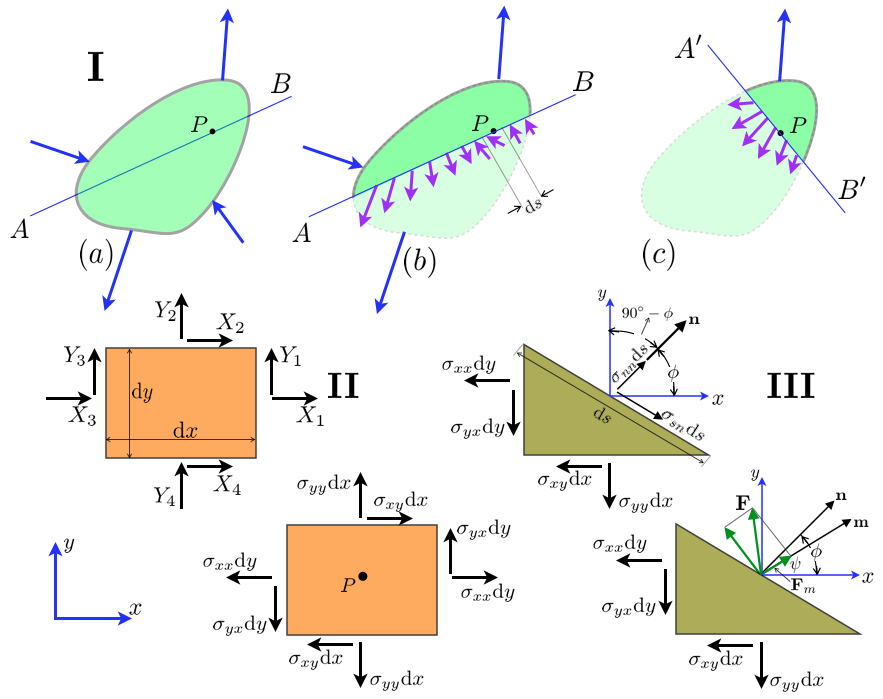
\includegraphics[width=5.8in]{VOLUMEN_1/03_Funciones_Lineales/Figuras/Figura3_1.jpg}
\caption{Tensor de Esfuerzos (\textit{stress}) en 2 dimensiones}
\label{figtensoresfuerzos2d}
\end{center}
\end{figure}

El cambio de signo se debe a lo inc�modo de la notaci�n: $\sigma_{4}\equiv\sigma_{y-y}$ ya que la normal de lado $4$ apunta en la direcci�n $-y$. Es importante tambi�n se�alar que los esfuerzos en cualquier punto contenido en el diferencial de �rea $\mathrm{d} A=\mathrm{d}x\mathrm{d}y$ deben ser considerado constantes, o lo que es lo mismo, que podemos hacer tender a cero el �rea del diferencial y con ello asociar los esfuerzos $\sigma_{ij}$ a un punto $P$ contenido en $\mathrm{d}A$ sobre la cual hemos calculado los esfuerzos.

En esta misma l�nea de razonamiento, nos podemos preguntar cu�l es la expresi�n de los esfuerzos cuando se miden respecto a una superficie
gen�rica, definida por un vector normal ${\bf n}$ (ver figura \ref{figtensoresfuerzos2d} cuadrante III). Es decir, queremos conocer los esfuerzos medidos en el punto $P$ y en la direcci�n ${\bf n}$, es decir, $\sigma_{nn}$. 

Por lo tanto, tendremos que:
\begin{eqnarray*}
x&\rightarrow&\sigma_{xx}\mathrm{d}y+\sigma_{xy}\mathrm{d}x=
\sigma_{nn}\mathrm{d}s\cos(\phi)+\sigma_{sn}\mathrm{d}s \ \mbox{sen}(\phi)\\
y&\rightarrow&\sigma_{yy}\mathrm{d}x+\sigma_{yx}\mathrm{d}y=
\sigma_{nn}\mathrm{d}s \ \mbox{sen}(\phi)-\sigma_{sn}\mathrm{d}s\cos(\phi)
\end{eqnarray*}

Ahora bien, dado que $\mathrm{d}y=\mathrm{d}s\cos(\phi)$ y $\mathrm{d}x=\mathrm{d}s \ \mathrm{sen}(\phi)$, entonces podemos expresar:
\begin{eqnarray*}
\sigma_{nn}  &  = &\sigma_{xx}\cos^{2}(\phi)+\sigma_{xy}\mbox{sen}(\phi)\cos(\phi)+\sigma_{yx}\mbox{sen}(\phi)\cos(\phi)+\sigma_{yy}
\mbox{sen}^{2}(\phi) \\
\sigma_{sn}  &  = &\sigma_{xx}\mbox{sen}(\phi)\cos(\phi)+\sigma_{xy}\mbox{sen}^{2}(\phi)-\sigma_{yx}\cos^{2}(\phi)-\sigma_{yy}\mbox{sen}(\phi)\cos(\phi)
\end{eqnarray*}
y si ahora nos damos cuenta que si construimos una matriz:
\[
A_{j}^{i}=\left(
\begin{array}
[c]{cc}
A_{n}^{x} &  A_{s}^{x}\\
A_{n}^{y}&  A_{s}^{y}
\end{array}
\right)  = 
\left(
\begin{array}
[c]{cc}
\cos(\phi) &  \operatorname{sen}(\phi)\\
\operatorname{sen}(\phi) & -\cos(\phi)
\end{array}
\right) \,,
\]
entonces:
\begin{align*}
\sigma_{nn}  &  =A_{n}^{x}A_{n}^{x}\sigma_{xx}+A_{n}^{x}A_{n}^{y}\sigma
_{xy}+A_{n}^{y}A_{n}^{x}\sigma_{yx}+A_{n}^{y}A_{n}^{y}\sigma_{yy}
\quad \Rightarrow \quad \sigma_{nn}=A_{n}^{i}A_{n}^{j}\sigma_{ij}\quad\text{con}i,j=x,y\\
& \\
\sigma_{sn}  &  =A_{s}^{x}A_{n}^{x}\sigma_{xx}+A_{s}^{x}A_{n}^{y}\sigma
_{xy}+A_{s}^{y}A_{n}^{x}\sigma_{yx}+A_{s}^{y}A_{n}^{y}\sigma_{yy}
\quad \Rightarrow \quad\sigma_{sn}=A_{s}^{i}A_{n}^{j}\sigma_{ij}\quad\text{con}i,j=x,y 
\end{align*}
es decir: 
\[
\sigma_{kl}=A_{k}^{i}A_{l}^{j}\sigma_{ij}\,, \quad \mbox{con} \quad  i,j,k,l=n,s \,.
\]
Como ya hemos mencionado, y veremos m�s adelante con m�s detalle, cualquier objeto que transforme como $\sigma_{kl}=A_{k}^{i}A_{l}^{j}\sigma_{ij}$ lo llamaremos tensor de segundo orden.

\begin{figure}[t]
\begin{center}
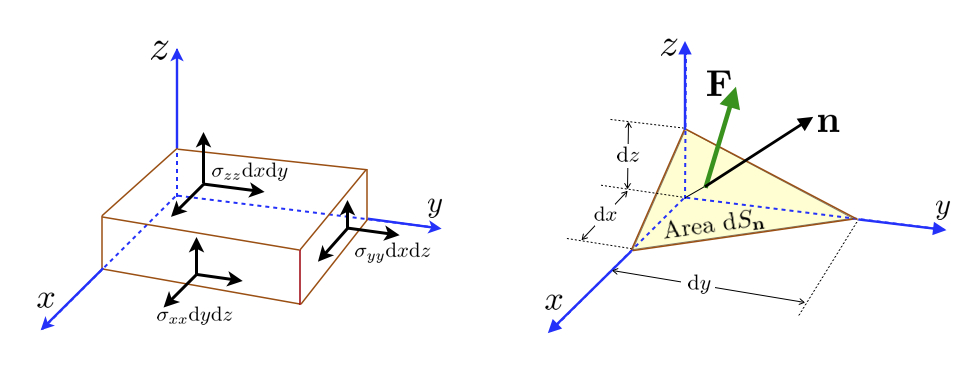
\includegraphics[width=6.0in]{VOLUMEN_1/03_Funciones_Lineales/Figuras/Figura3_2.jpg}
\caption{Tensor de Esfuerzos en 3 dimensiones}
\label{figtensoresfuerzos3d}
\end{center}
\end{figure}

\item {El tensor de esfuerzos  (caso 3D)}
\index{Tensor!Esfuerzo 3D}
Podemos  proceder como en el caso anterior estableciendo las siguientes condiciones de equilibrio:
\[
\sum{\bf F}_{i}^{ext}=0\quad\text{y}\quad\sum{\boldsymbol{\tau}}_{i}^{ext}=0\,,
\]
con ello construimos un volumen (c�bico) diferencial y construimos los
esfuerzos normales y tangenciales, los cuales ser�n:
\[
\sigma_{xx}\mathrm{d}y\mathrm{d}z\,, \quad
\sigma_{yy}\mathrm{d}x\mathrm{d}z\,, \quad
\sigma_{zz}\mathrm{d}x\mathrm{d}y\,, \quad
\sigma_{xz}\mathrm{d}x\mathrm{d}y\,, \quad
\sigma_{yz}\mathrm{d}x\mathrm{d}y\,, \quad
\sigma_{xy}\mathrm{d}x\mathrm{d}z\,.
\]

Siguiendo el mismo proceso que involucra imponer el equilibrio, es f�cil
demostrar que al igual que el caso anterior, el tensor de esfuerzos
$\sigma_{ij}$ cumple con:
\[
\sigma_{xz}=\sigma_{zx}\,, \quad
\sigma_{yz}=\sigma_{zy}\,, \quad
\sigma_{xy}=\sigma_{yx} \,.
\]

Tendremos $6$ componentes (tres normales y tres tangenciales)
independientes. Es decir, si bien el tensor de esfuerzos $\sigma_{ij}$ viene representado por una matriz $3\times3$ y por lo tanto tiene $9$ elementos, s�lo 6 son independientes. 

Vayamos ahora el caso general para un tensor de esfuerzos en un medio el�stico. Para ello construimos un tetraedro regular tal y como muestra la figura \ref{figtensoresfuerzos3d}, y sobre su cara gen�rica asociada a un vector normal ${\bf n}$ una fuerza ${\bf F}$:
\[
{\bf F}=F^{i}\text{\bf{i}}_{i}
=F_{x}\text{\bf{{i}}}+F_{y}\text{\bf{{j}}}+F_{z}
\text{\bf{{k}}}\,\, \Rightarrow \,\,  \left\{
\begin{array}
[c]{c}
F_{x}=\sigma_{xn}\mathrm{d}S_{n}\\
\\
F_{y}=\sigma_{yn}\mathrm{d}S_{n}\\
\\
F_{z}=\sigma_{zn}\mathrm{d}S_{n}
\end{array}
\right\} \,\, \Rightarrow \,\,   F^{i}=\sigma_{j}^{i}n^{j}\mathrm{d}S
\,\, \Rightarrow \,\,  {\bf F}=\boldsymbol{\sigma}\cdot\mathrm{d}{\bf S}\,.
\]
De �sta manera se especifica como la fuerza  act�a sobre un determinado elemento de superficie. Es claro que la condici�n de equilibrio se traduce en:
\begin{align*}
\sum F_{xi}  &  =0\,\, \Rightarrow \,\,  \sigma_{xn}\mathrm{d}S_{n}-\frac{1}{2}\sigma_{xx}\mathrm{d}y\ \mathrm{d}z-\frac{1}{2}\sigma_{xy}\mathrm{d}x\ \mathrm{d}z-\frac{1}{2}\sigma_{xz}\mathrm{d}x\ \mathrm{d}y=0 \,, \\
& \\
\sum F_{yi}  &  =0\,\, \Rightarrow \,\,  \sigma_{yn}\mathrm{d}S_{n}-\frac{1}{2}\sigma_{yx}\mathrm{d}y\ \mathrm{d}z-\frac{1}{2}\sigma_{yy}\mathrm{d}x\ \mathrm{d}z-\frac{1}{2}\sigma_{yz}\mathrm{d}x\ \mathrm{d}y=0 \,,  \\
& \\
\sum F_{zi}  &  =0\,\, \Rightarrow \,\,  \sigma_{zn}\mathrm{d}S_{n}-\frac{1}{2} \sigma_{zx}\mathrm{d}y\ \mathrm{d}z-\frac{1}{2}\sigma_{zy}\mathrm{d} x\ \mathrm{d}z-\frac{1}{2}\sigma_{zz}\mathrm{d}x\ \mathrm{d}y=0 \,.
\end{align*}

Si consideramos  la proyecci�n de $\mathrm{d}S_{n}$ sobre cada uno de los planos del sistema cartesiano tendremos:
\[
\left.
\begin{array}
[c]{c}
\mathrm{d}S^{n}\cos\left(  \text{\bf{{i}}};{\bf n}\right)  =\frac{1}
{2}\mathrm{d}y\ \mathrm{d}z=\mathrm{d}S^{n}\ A_{n}^{x}\\
\\
\mathrm{d}S^{n}\cos\left(  \text{\bf{{j}}};{\bf n}\right)  =\frac{1}
{2}\mathrm{d}x\ \mathrm{d}z=\mathrm{d}S^{n}\ A_{n}^{y}\\
\\
\mathrm{d}S^{n}\cos\left(  \text{\bf{{k}}};{\bf n}\right)  =\frac{1}
{2}\mathrm{d}x\ \mathrm{d}y=\mathrm{d}S^{n}\ A_{n}^{z}
\end{array}
\right\}  \,\, \Rightarrow \,\,  \sigma_{xn}=\sigma_{xx}A_{n}^{x}+\sigma_{xy}
A_{n}^{y}+\sigma_{xz}A_{n}^{z}\,,
\]
y equivalentemente:
\[
\sigma_{yn}=\sigma_{yx}A_{n}^{x}+\sigma_{yy}A_{n}^{y}+\sigma_{yz}A_{n}^{z} \quad\text{y}\quad
\sigma_{zn}=\sigma_{zx}A_{n}^{x}+\sigma_{zy}A_{n}^{y}+\sigma_{zz}A_{n}^{z}\,,
\]
las cuales se conocen como las relaciones de Cauchy. Estas relaciones  representan los
esfuerzos sobre la superficie con normal ${\bf n}$. 

Ahora bien, dado que: ${\bf F}=\boldsymbol{\sigma}\mathrm{d}{S}$ es una relaci�n vectorial
podemos proyectar en la direcci�n $\hat{\bf u}_{m}$:
\[
\hat{\bf  u}_{m}\cdot {\bf F}   =\hat{\bf u}_{m}\cdot \left( \boldsymbol{\sigma}\mathrm{d}{ S} \right)\,\, \Rightarrow \,\,   F^{m}=\sigma_{n}^{m}\mathrm{d}S^{n}=
\left(\sigma_{i}^{m}A_{n}^{i}\right)  \mathrm{d}S^{n}=\left(  \sigma_{i}^{m}
A_{n}^{i}\right)  \mathrm{d}S^{n}\,,
\]
por lo tanto:
\[
\sigma_{mn}\mathrm{d}S^{n}   =\left(  \sigma_{mi}A_{n}^{i}\right)
\mathrm{d}S^{n}\,\, \Rightarrow \,\,  \sigma_{mn}\mathrm{d}S^{n}=\left(  \sigma_{ki}A_{m}^{k}A_{n}^{i}\right)  \mathrm{d}S^{n}\,,
\quad\text{con } i,j=x,y,z \,.
\]
Una vez m�s, podemos ver  que transforma como un tensor.

\item {El Tensor de inercia}
\label{TensorInercia}
Consideremos el caso de un sistema de $n$ part�culas. La cantidad de
movimiento angular para este sistema vendr� dada por:
\[
{\bf L}=\sum_{i}m_{\left(  i\right)  }\left(  {\bf r}_{\left(  i\right)
}\times{\bf v}_{\left(  i\right)  }\right) \,,
\]
donde hemos indicado que la $i-$�sima part�cula que est� en la
posici�n $\bf{r}_{\left(  i\right)  }$ tiene una velocidad ${\bf v}_{\left(  i\right) }$. 

Si las distancias entre las part�culas, y entre las part�culas con el origen de coordenadas, es constante, podremos expresar la velocidad de cada una de ellas como:
\[
{\bf v}_{\left(  i\right)  }=\boldsymbol{\omega}\times{\bf r}_{\left(  i\right)}\,,\quad \mbox{�Por qu�?}
\]

Donde $\boldsymbol{\omega}$ es la velocidad angular instant�nea del sistema. Entonces tendremos que:
\[
{\bf L}=\sum_{i} m_{\left(  i\right)  }\left[  {\bf r}_{\left(  i\right)
}\times\left(  \boldsymbol{\omega}\times{\bf r}_{\left(  i\right)  }\right)  \right]
=\sum_{i}m_{\left(  i\right)  }\left[  \boldsymbol{\omega}\left(  {\bf r}_{\left(
i\right)  }\cdot{\bf r}_{\left(  i\right)  }\right)  -{\bf r}_{\left(
i\right)  }\left(  \boldsymbol{\omega}\cdot{\bf r}_{\left(  i\right)  }\right)
\right] \,,
\]
y para cada part�cula se cumple que las componentes de la cantidad de movimiento angular ser�n:
\[
L^{k}=\sum_{i}m_{\left(  i\right)  }\left[  \omega^{k}\left(  r_{\left(
i\right)  }^{m}r_{\left(  i\right)  m}\right)  -r_{\left(  i\right)  }
^{k}\left(  \omega^{m}r_{\left(  i\right)  m}\right)  \right]\,.
\]

Si vemos que $\omega_{\left(  i\right)  }^{k}=\delta_{l}^{k}\omega_{\left(
i\right)  }^{l}$ entonces:
\[
L^{k}=  \sum_{i}m_{\left(  i\right)  }\left[  \delta_{l}^{k}\omega
^{l}\left(  r_{\left(  i\right)  }^{m}r_{\left(  i\right)  m}\right)
-r_{\left(  i\right)  }^{k}\left(  \omega^{m}r_{\left(  i\right)  m}\right)
\right]   =\omega_{\left(  i\right)  }^{l}\underset{I_{l}^{k}
}{\underbrace{\left[  \sum_{i}m_{\left(  i\right)  }\left(  \delta_{l}
^{k}\left(  r_{\left(  i\right)  }^{m}r_{\left(  i\right)  m}\right)
-r_{\left(  i\right)  }^{k}\left(  r_{\left(  i\right)  l}\right)  \right)
\right] }}
\]
es decir:
\[
L^{k}=\omega_{\left(  i\right)  }^{l}I_{l}^{k}\,, \quad\text{donde: } \quad\, 
I_{l}^{k}=\sum_{i}m_{\left(  i\right)  }\left(  \delta_{l}^{k}\left(  r_{\left(
i\right)  }^{m}r_{\left(  i\right)  m}\right)  -r_{\left(  i\right)  }
^{k}\left(  r_{\left(  i\right)  l}\right)  \right)\,.
\]

El objeto $I_{l}^{k}$ se conoce como el tensor de inercia y corresponde a $9$ cantidades (s�lo $6$ son independientes porque es un tensor sim�trico). En coordenadas cartesianas se ver� de la siguiente forma:
\[
I_{l}^{k}=\left(
\begin{array}
[c]{lllll}
I_{xx}   &  & I_{xy}  &  &I_{xz}   \\
            &  &            &  & \\
I_{yx}   &  & I_{yy}  &  &I_{yz}  \\
            &  &            &  & \\
I_{zx}   &  & I_{zy}  &  & I_{zz}
\end{array}
\right) = 
\left(
\begin{array}
[c]{lllll}
\sum_{i}m_{(i)}\left(y_{(i)} ^{2}+z_{(i)}^{2} \right)  &  & -\sum_{i}m_{(i)  }\left(x_{(i)}y_{(i)}\right)             &  & -\sum_{i}m_{(i)}\left(x_{(i)}z_{(i)}\right)  \\
                                                                             &  &                                                                            &  & \\
-\sum_{i} m_{(i)}\left(x_{(i)}y_{(i)}\right)                &  & \sum_{i}m_{(i)}\left(x_{(i)}^{2}+z_{(i)}^{2}\right)  &  & -\sum_{i}m_{(i)}\left(y_{(i)}z_{(i)}\right)  \\
                                                                             &  &                                                                            &  & \\
-\sum_{i}m_{(i)}\left(x_{(i)}z_{(i)}\right)                 &  &-\sum_{i}m_{(i)}\left(y_{(i)}z_{(i)}\right)                 &  & \sum_{i}m_{(i)}\left(x_{(i)}^{2} +y_{(i)}^{2}\right)
\end{array}
\right) 
\]
Por ahora, nos contentaremos con esta construcci�n y en los ejercicios le propondremos que muestre que es un tensor. 


\item {\bf Energ�a libre para un medio el�stico} 

Consideremos el siguiente par de tensores provenientes  de la teor�a de elasticidad:
\[
u_{ik}=\frac{1}{2}\left(  \partial_{k}\ u_{i}+\partial_{i}\ u_{k}\right)
\equiv\frac{1}{2}\left(  \frac{\partial u_{i}}{\partial x^{k}}
+\frac{\partial u_{k}}{\partial x^{i}}\right)\,, \quad\left(  u_{k}
^{i}\right)  ^{0}=u_{k}^{i}-\frac{1}{3}u_{m}^{m}\ \delta_{k}^{i}\,,
\]
y construyamos el tensor de esfuerzos como: $p_{j}^{i}=2\lambda\left(  u_{j}^{i}\right)  ^{0}+Ku_{l}^{l}\ \delta_{j}^{i}$. 

Calculemos la energ�a libre para el medio el�stico, definida como: $F=\frac{1}{2}p_{j}^{i}u_{i}^{j}$.  

Tenemos que:
\[
p_{j}^{i}=2\lambda\left(  u_{j}^{i}\right)  ^{0}+Ku_{l}^{l}\ \delta_{j}
^{i}=2\lambda\left(  u_{j}^{i}-\frac{1}{3}u_{m}^{m}\ \delta_{j}^{i}\right)
+Ku_{l}^{l}\ \delta_{j}^{i}=2\lambda u_{j}^{i}+u_{l}^{l}\delta_{j}^{i}\left(
K-\frac{2\lambda}{3}\right)\,,
\]
donde: $u_{m}^{m}=\frac{1}{2}\left(  \partial^{m}\ u_{m}+\partial_{m}
\ u^{m}\right)  =\partial^{m}\ u_{m}$, con lo cual:

\begin{align*}
F  & =\frac{1}{2}p_{j}^{i}u_{i}^{j}=\frac{1}{2}\left(  2\lambda u_{j}
^{i}+u_{l}^{l}\delta_{j}^{i}\left(  K-\frac{2\lambda}{3}\right)  \right)
u_{i}^{j}=\left(  \lambda u_{j}^{i}u_{i}^{j}+u_{l}^{l}\delta_{j}^{i}u_{i}
^{j}\left(  \frac{1}{2}K-\frac{\lambda}{3}\right)  \right)  \\
& =\lambda\left(  u_{1}^{i}u_{i}^{1}+u_{2}^{i}u_{i}^{2}+u_{3}^{i}u_{i}
^{3}\right)  +\left(  \frac{1}{2}K-\frac{\lambda}{3}\right)  \left(  u_{l}
^{l}\right)  ^{2}\\
& =\lambda\left(  \left(  u_{1}^{1}u_{1}^{1}+u_{1}^{2}u_{2}^{1}+u_{1}^{3}
u_{3}^{1}\right)  +\left(  u_{2}^{1}u_{1}^{2}+u_{2}^{2}u_{2}^{2}+u_{2}
^{3}u_{3}^{2}\right)  +\left(  u_{3}^{1}u_{1}^{3}+u_{3}^{2}u_{2}^{3}+u_{3}
^{3}u_{3}^{3}\right)  \right)  +\left(  \frac{1}{2}K-\frac{\lambda}{3}\right)
\left(  u_{l}^{l}\right)  ^{2}\\
& =\lambda\left(  \left(  u_{1}^{1}\right)  ^{2}+\left(  u_{2}^{2}\right)
^{2}+\left(  u_{3}^{3}\right)  ^{2}+2\left(  u_{2}^{1}u_{1}^{2}+u_{3}^{2}
u_{2}^{3}+u_{1}^{3}u_{3}^{1}\right)  \right)  +\left(  \frac{1}{2}
K-\frac{\lambda}{3}\right)  \left(  u_{l}^{l}\right)  ^{2}\\
& =\left(  \frac{1}{2}K+\frac{2\lambda}{3}\right)  \left(  u_{l}^{l}\right)
^{2}+2\lambda\left(  u_{2}^{1}u_{1}^{2}+u_{3}^{2}u_{2}^{3}+u_{1}^{3}u_{3}
^{1}\right)  \\
& =\left(  \frac{1}{2}K+\frac{2\lambda}{3}\right)  \left(  \partial_{x}
u_{x}+\partial_{y}u_{y}+\partial_{z}u_{z}\right)  ^{2}+2\lambda\left(
\partial_{x}u_{y}\partial_{y}u_{x}+\partial_{y}u_{z}\partial_{z}u_{y}
+\partial_{z}u_{x}\partial_{x}u_{z}\right)\,.
\end{align*}

\end{enumerate}




\end{enumerate}

\newpage
\subsection{{\color{red}Practicando con Maxima}}
\subsubsection{Tensores y Maxima}
{\bf Maxima}  presenta dos paquetes para la manipulaci�n de tensores, paquetes en constante desarrollo todav�a. Estos paquetes son {\bf ctensor}, manipulaci�n de componentes y el paquete {\bf itensor}, manipulaci�n indexada. En la manipulaci�n por componentes los tensores se representan por arreglos o matrices. En la manipulaci�n indexada los tensores se representan por funciones de sus �ndices covariantes, contravariantes y de derivadas.

Los �ndices covariantes se especifican mediante una lista que ser� el primer argumento del objeto indexado, siendo los �ndices contravariantes otra lista que ser� el segundo argumento del mismo objeto indexado. Si al objeto indexado le falta cualquiera de estos grupos de �ndices, entonces se le asignar� al argumento correspondiente la lista vac�a $[\ ]$. As�, $g([a,b],[c])$ representa un objeto indexado llamado $g$, el cual tiene dos �ndices covariantes $(a,b)$, un �ndice contravariante $(c)$ y no tiene �ndices de derivadas, es decir, $g_{ab}^c$

%%%%%% INPUT:
\begin{minipage}[t]{8ex}
{\color{red}\bf \begin{verbatim} (%i1) 
\end{verbatim}}
\end{minipage}
\begin{minipage}[t]{\textwidth}{\color{blue}
\begin{verbatim}
load(itensor)$
\end{verbatim}}
\end{minipage}

%%%%%% INPUT:
\begin{minipage}[t]{8ex}
{\color{red}\bf \begin{verbatim} (%i2) 
\end{verbatim}}
\end{minipage}
\begin{minipage}[t]{\textwidth}{\color{blue}
\begin{verbatim}
imetric(g);
\end{verbatim}}
\end{minipage}

%%%%%% INPUT:
\begin{minipage}[t]{8ex}
{\color{red}\bf \begin{verbatim} (%i3) 
\end{verbatim}}
\end{minipage}
\begin{minipage}[t]{\textwidth}{\color{blue}
\begin{verbatim}
ishow(g([j,k],[])*g([i,l],[])*a([],[i,j]))$
\end{verbatim}}
\end{minipage}

%%% OUTPUT:
\begin{math}\displaystyle \parbox{8ex}{\color{labelcolor}(\%t3) }
a^{i\,j}\,g_{j\,k}\,g_{i\,l}
\end{math}

%%%%%% INPUT:
\begin{minipage}[t]{8ex}
{\color{red}\bf \begin{verbatim} (%i4) 
\end{verbatim}}
\end{minipage}
\begin{minipage}[t]{\textwidth}{\color{blue}
\begin{verbatim}
ishow(contract(%))$
\end{verbatim}}
\end{minipage}

%%% OUTPUT:
\begin{math}\displaystyle \parbox{8ex}{\color{labelcolor}(\%t4) }
a_{k\,l}
\end{math}

%%%%%% INPUT:
\begin{minipage}[t]{8ex}
{\color{red}\bf \begin{verbatim} (%i5) 
\end{verbatim}}
\end{minipage}
\begin{minipage}[t]{\textwidth}{\color{blue}
\begin{verbatim}
ishow(kdelta([i],[k])*a([k,l],[]))$
\end{verbatim}}
\end{minipage}

%%% OUTPUT:
\begin{math}\displaystyle \parbox{8ex}{\color{labelcolor}(\%t5) }
\delta_{i}^{k}\,a_{k\,l}
\end{math}

%%%%%% INPUT:
\begin{minipage}[t]{8ex}
{\color{red}\bf \begin{verbatim} (%i6) 
\end{verbatim}}
\end{minipage}
\begin{minipage}[t]{\textwidth}{\color{blue}
\begin{verbatim}
ishow(contract(%))$
\end{verbatim}}
\end{minipage}

%%% OUTPUT:
\begin{math}\displaystyle \parbox{8ex}{\color{labelcolor}(\%t6) }
a_{i\,l}
\end{math}
\newline

La identidad $\delta_i^j\delta_j^i=3$

%%%%%% INPUT:
\begin{minipage}[t]{8ex}
{\color{red}\bf \begin{verbatim} (%i7) 
\end{verbatim}}
\end{minipage}
\begin{minipage}[t]{\textwidth}{\color{blue}
\begin{verbatim}
ishow(contract(kdelta([i], [j])*kdelta([j], [i])))$
\end{verbatim}}
\end{minipage}

%%% OUTPUT:
\begin{math}\displaystyle \parbox{8ex}{\color{labelcolor}(\%t7) }
kdelta
\end{math}

%%%%%% INPUT:
\begin{minipage}[t]{8ex}
{\color{red}\bf \begin{verbatim} (%i8) 
\end{verbatim}}
\end{minipage}
\begin{minipage}[t]{\textwidth}{\color{blue}
\begin{verbatim}
ishow(ev(%,kdelta))$
\end{verbatim}}
\end{minipage}

%%% OUTPUT:
\begin{math}\displaystyle \parbox{8ex}{\color{labelcolor}(\%t8) }
3
\end{math}
\newline

El s�mbolo de Levi-Civita:

%%%%%% INPUT:
\begin{minipage}[t]{8ex}
{\color{red}\bf \begin{verbatim} (%i9) 
\end{verbatim}}
\end{minipage}
\begin{minipage}[t]{\textwidth}{\color{blue}
\begin{verbatim}
levi_civita([1, 2, 3]);levi_civita([1, 3, 2]);levi_civita([3, 3, 2]);
\end{verbatim}}
\end{minipage}

%%% OUTPUT:
\begin{math}\displaystyle \parbox{8ex}{\color{labelcolor}(\%o9) }
1
\end{math}

%%% OUTPUT:
\begin{math}\displaystyle \parbox{8ex}{\color{labelcolor}(\%o10) }
-1
\end{math}

%%% OUTPUT:
\begin{math}\displaystyle \parbox{8ex}{\color{labelcolor}(\%o11) }
0
\end{math}


%%%%%% INPUT:
\begin{minipage}[t]{8ex}
{\color{red}\bf \begin{verbatim} (%i12) 
\end{verbatim}}
\end{minipage}
\begin{minipage}[t]{\textwidth}{\color{blue}
\begin{verbatim}
expr:ishow('levi_civita([],[i,j,k])*'levi_civita([i,j,k],[]))$
\end{verbatim}}
\end{minipage}

%%% OUTPUT:
\begin{math}\displaystyle \parbox{8ex}{\color{labelcolor}(\%t12) }
\varepsilon^{i\,j\,k}\,\varepsilon_{i\,j\,k}
\end{math}
\newline

Aqu� es necesario utilizar la funci�n {\bf lc2kdt( )} que 
simplifica expresiones que contengan el s�mbolo de Levi-Civita, para convertirlas en expresiones con la delta de Kronecker siempre que esto sea posible.\footnote{En ocaciones, la funci�n  {\bf lc2kdt( )}  hace uso del tensor m�trico. Si el tensor m�trico no fue previamente definido con {\bf imetric}, se obtiene un mensaje de error.}


%%%%%% INPUT:
\begin{minipage}[t]{8ex}
{\color{red}\bf \begin{verbatim} (%i13) 
\end{verbatim}}
\end{minipage}
\begin{minipage}[t]{\textwidth}{\color{blue}
\begin{verbatim}
ishow(lc2kdt(expr))$
\end{verbatim}}
\end{minipage}

%%% OUTPUT:
\begin{math}\displaystyle \parbox{8ex}{\color{labelcolor}(\%t13) }
\left(\delta_{i}^{k}\,\delta_{j}^{i}-3\,\delta_{j}^{k}\right)\,
 \delta_{k}^{j}+\left(\delta_{i}^{j}\,\delta_{j}^{k}-3\,\delta_{i}^{k
 }\right)\,\delta_{k}^{i}-3\,\delta_{i}^{j}\,\delta_{j}^{i}+27
\end{math}

%%%%%% INPUT:
\begin{minipage}[t]{8ex}
{\color{red}\bf \begin{verbatim} (%i14) 
\end{verbatim}}
\end{minipage}
\begin{minipage}[t]{\textwidth}{\color{blue}
\begin{verbatim}
ishow(contract(expand(%)))$
\end{verbatim}}
\end{minipage}

%%% OUTPUT:
\begin{math}\displaystyle \parbox{8ex}{\color{labelcolor}(\%t14) }
27-7\,\delta
\end{math}

%%%%%% INPUT:
\begin{minipage}[t]{8ex}
{\color{red}\bf \begin{verbatim} (%i15) 
\end{verbatim}}
\end{minipage}
\begin{minipage}[t]{\textwidth}{\color{blue}
\begin{verbatim}
ishow(ev(%,kdelta))$
\end{verbatim}}
\end{minipage}

%%% OUTPUT:
\begin{math}\displaystyle \parbox{8ex}{\color{labelcolor}(\%t15) }
6
\end{math}

%%%%%% INPUT:
\begin{minipage}[t]{8ex}
{\color{red}\bf \begin{verbatim} (%i16) 
\end{verbatim}}
\end{minipage}
\begin{minipage}[t]{\textwidth}{\color{blue}
\begin{verbatim}
kill(all)$
\end{verbatim}}
\end{minipage}

\subsubsection{Transformaci�n de tensores y Maxima}
Como ya mencionamos, {\bf Maxima} contiene un paquete para manipular componentes de tensores: {\bf ctensor}. La manipulaci�n en componentes se realiza en t�rminos de matrices. La m�trica se almacena en la matriz $\mathrm{lg}$ y la m�trica inversa se obtiene y almacena en la matriz $\mathrm{ug}$.

En un ejemplo visto con anterioridad se especificaba las componentes de un tensor en coordenadas cartesianas, esto es:
\[
\mathrm{To}=T_{j}^{i}=\left(
\begin{array}
[c]{ccc}
2 & 1 & 3\\
2 & 3 & 4\\
1 & 2 & 2
\end{array}
\right)\,, \quad \mbox{en la base: }
\left\{  \left|  \mathrm{e}_{1}\right> ,\left|  \mathrm{e}_{2}\right> ,\left|  \mathrm{e}_{3}\right> \right\}
\equiv\left\{  \left|  \mathrm{i}\right> ,\left|  \mathrm{j}\right> ,\left|  \mathrm{k}\right> \right\} \,.
\]

Para luego representarlo en la nueva base:   
$ \left|  \mathrm{\tilde{w}}_{1}\right> =\left|  \mathrm{i}\right>$, $\left|  \mathrm{\tilde{w}}_{2}\right>=\left|  \mathrm{i}\right> +\left|  \mathrm{j}\right> $ y 
$\left|  \mathrm{\tilde{w}}_{3}\right>=\left|  \mathrm{i}\right>+\left|  \mathrm{j}\right> +\left|  \mathrm{k}\right> $.
Entonces necesitamos  calcular:
\[
\tilde{T}_{m}^{k} =\frac{\partial \tilde{x}^{k}}{\partial x^{i}}
\frac{\partial x^{j}}{\partial \tilde{x}^{m}}\ T_{j}^{i}
\,\, \Rightarrow \,\, \mathrm{Tn}=\alpha\beta\mathrm{To}=
\]

Como vimos cuando hac�amos los c�lculos:
\[
\alpha=\frac{\partial \tilde{x}^{k}}{\partial x^{i}}=
\left(
\begin{array}
[c]{rrr}
1 & -1 & 0\\
0 & 1 & -1\\
0 & 0 & 1
\end{array}
\right)\,, \qquad
\beta=\frac{\partial x^{i}}{\partial \tilde{x}^{k}}=
\left(
\begin{array}
[c]{lll}
1 & 1 & 1\\
0 & 1 & 1\\
0 & 0 & 1
\end{array}
\right)\,.
\]

Respetando ``la concatenaci�n interna de �ndices'' podemos realizar la multiplicaci�n de matrices.  

%%%%%% INPUT:
\begin{minipage}[t]{8ex}
{\color{red}\bf \begin{verbatim} (%i1) 
\end{verbatim}}
\end{minipage}
\begin{minipage}[t]{\textwidth}{\color{blue}
\begin{verbatim}
To:matrix([2,1,3],[2,3,4],[1,2,2]);
\end{verbatim}}
\end{minipage}

%%% OUTPUT:
\begin{math}\displaystyle \parbox{8ex}{\color{labelcolor}(\%o1) }
\begin{pmatrix}2 & 1 & 3 \\ 2 & 3 & 4 \\ 1 & 2 & 2 \\ \end{pmatrix}
\end{math}

%%%%%% INPUT:
\begin{minipage}[t]{8ex}
{\color{red}\bf \begin{verbatim} (%i2) 
\end{verbatim}}
\end{minipage}
\begin{minipage}[t]{\textwidth}{\color{blue}
\begin{verbatim}
alpha:matrix([1,-1,0],[0,1,-1],[0,0,1]);
\end{verbatim}}
\end{minipage}

%%% OUTPUT:
\begin{math}\displaystyle \parbox{8ex}{\color{labelcolor}(\%o2) }
\begin{pmatrix}1 & -1 & 0 \\ 0 & 1 & -1 \\ 0 & 0 & 1 \\ 
 \end{pmatrix}
\end{math}

%%%%%% INPUT:
\begin{minipage}[t]{8ex}
{\color{red}\bf \begin{verbatim} (%i3) 
\end{verbatim}}
\end{minipage}
\begin{minipage}[t]{\textwidth}{\color{blue}
\begin{verbatim}
beta:matrix([1,1,1],[0,1,1],[0,0,1]);
\end{verbatim}}
\end{minipage}

%%% OUTPUT:
\begin{math}\displaystyle \parbox{8ex}{\color{labelcolor}(\%o3) }
\begin{pmatrix}1 & 1 & 1 \\ 0 & 1 & 1 \\ 0 & 0 & 1 \\ \end{pmatrix}
\end{math}

%%%%%% INPUT:
\begin{minipage}[t]{8ex}
{\color{red}\bf \begin{verbatim} (%i4) 
\end{verbatim}}
\end{minipage}
\begin{minipage}[t]{\textwidth}{\color{blue}
\begin{verbatim}
Tn:alpha.To.beta;
\end{verbatim}}
\end{minipage}

%%% OUTPUT:
\begin{math}\displaystyle \parbox{8ex}{\color{labelcolor}(\%o4) }
\begin{pmatrix}0 & -2 & -3 \\ 1 & 2 & 4 \\ 1 & 3 & 5 \\ 
 \end{pmatrix}
 \end{math}
\newline

Una vez que hemos calculado el nuevo tensor $\mathrm{Tn}={\tilde T}_i^j$ en la nueva base, podemos calcular: ${\tilde T}^{ij}$, ${\tilde T}_{ij}$. Pero podemos utilizar la m�trica para las coordenadas nuevas y con el paquete {\bf ctensor} hacer las respectivas contracciones. 

%%%%%% INPUT:
\begin{minipage}[t]{8ex}
{\color{red}\bf \begin{verbatim} (%i5) 
\end{verbatim}}
\end{minipage}
\begin{minipage}[t]{\textwidth}{\color{blue}
\begin{verbatim}
load(ctensor)$
\end{verbatim}}
\end{minipage}

%%%%%% INPUT:
\begin{minipage}[t]{8ex}
{\color{red}\bf \begin{verbatim} (%i6) 
\end{verbatim}}
\end{minipage}
\begin{minipage}[t]{\textwidth}{\color{blue}
\begin{verbatim}
ct_coordsys(cartesian3d)$
\end{verbatim}}
\end{minipage}
\newline

Introducimos la m�trica ${\tilde g}_{ik}$:

%%%%%% INPUT:
\begin{minipage}[t]{8ex}
{\color{red}\bf \begin{verbatim} (%i7) 
\end{verbatim}}
\end{minipage}
\begin{minipage}[t]{\textwidth}{\color{blue}
\begin{verbatim}
lg:matrix([1,1,1],[1,2,2],[1,2,3]);
\end{verbatim}}
\end{minipage}

%%% OUTPUT:
\begin{math}\displaystyle \parbox{8ex}{\color{labelcolor}(\%o7) }\begin{pmatrix}1 & 1 & 1 \\ 1 & 2 & 2 \\ 1 & 2 & 3 \\ \end{pmatrix} \end{math}
\newline

Para tener la m�trica inversa ${\tilde g}^{ik}$ escribimos:

%%%%%% INPUT:
\begin{minipage}[t]{8ex}
{\color{red}\bf \begin{verbatim} (%i8) 
\end{verbatim}}
\end{minipage}
\begin{minipage}[t]{\textwidth}{\color{blue}
\begin{verbatim}
cmetric()$
\end{verbatim}}
\end{minipage}

%%%%%% INPUT:
\begin{minipage}[t]{8ex}
{\color{red}\bf \begin{verbatim} (%i9) 
\end{verbatim}}
\end{minipage}
\begin{minipage}[t]{\textwidth}{\color{blue}
\begin{verbatim}
ug;
\end{verbatim}}
\end{minipage}

%%% OUTPUT:
\begin{math}\displaystyle \parbox{8ex}{\color{labelcolor}(\%o9) }\begin{pmatrix}2 & -1 & 0 \\ -1 & 2 & -1 \\ 0 & -1 & 1 \\ 
 \end{pmatrix}
\end{math}
\newline

Para calcular ${\tilde T}_{ij}={\tilde g}_{ik}{\tilde T}_j^{k}$ hacemos lo siguiente:

%%%%%% INPUT:
\begin{minipage}[t]{8ex}
{\color{red}\bf \begin{verbatim} (%i10) 
\end{verbatim}}
\end{minipage}
\begin{minipage}[t]{\textwidth}{\color{blue}
\begin{verbatim}
lg.Tn;
\end{verbatim}}
\end{minipage}

%%% OUTPUT:
\begin{math}\displaystyle \parbox{8ex}{\color{labelcolor}(\%o10) }\begin{pmatrix}2 & 3 & 6 \\ 4 & 8 & 15 \\ 5 & 11 & 20 \\ 
 \end{pmatrix}
\end{math}
\newline

Y para calcular ${\tilde T}^{ij}={\tilde T}^i_{k}{\tilde g}^{kj}$ procedemos as�:

%%%%%% INPUT:
\begin{minipage}[t]{8ex}
{\color{red}\bf \begin{verbatim} (%i11) 
\end{verbatim}}
\end{minipage}
\begin{minipage}[t]{\textwidth}{\color{blue}
\begin{verbatim}
Tn.ug;
\end{verbatim}}
\end{minipage}

%%% OUTPUT:
\begin{math}\displaystyle \parbox{8ex}{\color{labelcolor}(\%o11) }\begin{pmatrix}2 & -1 & -1 \\ 0 & -1 & 2 \\ -1 & 0 & 2 \\ 
 \end{pmatrix}
\end{math}

%%%%%% INPUT:
\begin{minipage}[t]{8ex}
{\color{red}\bf \begin{verbatim} (%i12) 
\end{verbatim}}
\end{minipage}
\begin{minipage}[t]{\textwidth}{\color{blue}
\begin{verbatim}
kill(all)$
\end{verbatim}}
\end{minipage}
\newline

Es posible, y a manera de completar esta primer acercamiento con la librer�a de tensores,  calcular la m�trica a partir de una transformaci�n de coordenadas, como vimos en la secci�n anterior, ejemplo \ref{Repensandolascomponentes}. Escribimos las coordenadas que queremos utilizar, en este caso esf�ricas, utilizando la funci�n {\bf ct coordsys}.

%%%%%% INPUT:
\begin{minipage}[t]{8ex}
{\color{red}\bf \begin{verbatim} (%i1) 
\end{verbatim}}
\end{minipage}
\begin{minipage}[t]{\textwidth}{\color{blue}
\begin{verbatim}
load(ctensor)$
\end{verbatim}}
\end{minipage}
\newline

%%%%%% INPUT:
\begin{minipage}[t]{8ex}
{\color{red}\bf \begin{verbatim} (%i2) 
\end{verbatim}}
\end{minipage}
\begin{minipage}[t]{\textwidth}{\color{blue}
\begin{verbatim}
ct_coordsys([r*sin(theta)*cos(phi),r*sin(theta)*sin(phi),r*cos(theta),[r,theta,phi]])$
\end{verbatim}}
\end{minipage}
\newline

Y le pedimos al programa que calcule el tensor m�trico, al que le asigna el nombre {\bf lg}.

%%%%%% INPUT:
\begin{minipage}[t]{8ex}
{\color{red}\bf \begin{verbatim} (%i3) 
\end{verbatim}}
\end{minipage}
\begin{minipage}[t]{\textwidth}{\color{blue}
\begin{verbatim}
cmetric()$
\end{verbatim}}
\end{minipage}
\newline

El tensor m�trico $g_{ij}$ es entonces

%%%%%% INPUT:
\begin{minipage}[t]{8ex}
{\color{red}\bf \begin{verbatim} (%i4) 
\end{verbatim}}
\end{minipage}
\begin{minipage}[t]{\textwidth}{\color{blue}
\begin{verbatim}
lg:trigsimp(lg);
\end{verbatim}}
\end{minipage}

%%% OUTPUT:
\begin{math}\displaystyle \parbox{8ex}{\color{labelcolor}(\%o4) }\begin{pmatrix}1 & 0 & 0 \\ 0 & r^2 & 0 \\ 0 & 0 & r^2\,\sin ^2
 \theta \\ \end{pmatrix}
\end{math}
\newline

Y la m�trica inversa $g^{ij}$, el programa la identifica con la etiqueta  {\bf ug}

%%%%%% INPUT:
\begin{minipage}[t]{8ex}
{\color{red}\bf \begin{verbatim} (%i5) 
\end{verbatim}}
\end{minipage}
\begin{minipage}[t]{\textwidth}{\color{blue}
\begin{verbatim}
trigsimp(ug);
\end{verbatim}}
\end{minipage}

%%% OUTPUT:
\begin{math}\displaystyle \parbox{8ex}{\color{labelcolor}(\%o5) }\begin{pmatrix}1 & 0 & 0 \\ 0 & \frac{1}{r^2} & 0 \\ 0 & 0 & \frac{
 1}{r^2\,\sin ^2\theta} \\ \end{pmatrix}
\end{math}

\begin{center}
{\color{red}\rule{15.8cm}{0.4mm}}
\end{center}

\subsection{{\color{OliveGreen}Ejercicios}}

\begin{enumerate}
\item Si $A_{ijk}$ es un tensor covariante de orden 3 y $B^{lmno}$ un tensor contravariante de orden 4, pruebe que $A_{ijk}B^{jkno}$ es un tensor mixto de orden 3.

\item Dados los tensores:
\[
R^{i}_j=\left(
\begin{array}
[c]{ccc}
1/2  & 1    & 3/2   \\
2     & 5/2 &  3   \\
7/2  & 4    & 9/2 
\end{array}
\right) \,, \quad 
T^i= 
\left(
\begin{array}
[c]{c}
1/ 3     \\
2/3    \\
1   
\end{array}
\right) \,, \quad 
g^{i}_j=g^{ij}=g_{ij}=\left(
\begin{array}
[c]{ccc}
1 & 0 & 0   \\
0 & 1 & 0   \\
0 & 0 & 1 
\end{array}
\right) \,.
\] 
Encuentre:
\begin{enumerate}
\item La parte sim�trica $S^{i}_j$ y antisim�trica $A^{i}_j$ de $R^{i}_j$.
\item $R_{kj}=g_{ik}R^i_j$, $R^{ki}=g^{jk}R^i_j$, $T_{j}=g_{ij}T^i$ �Qu� se concluye de estos c�lculos?
\item $R^i_jT_i$, $R^i_jT^j$, $R^i_jT_iT^j$.
\item $R^i_j S_i^j$, $R^i_j A_i^j$, $A_i^jT^i$, $A_i^jT^iT_j$.
\item $R^i_j-2\delta^i_jR^l_l$, $(R^i_j-2\delta^i_jR^l_l)T_i$, $(R^i_j-2\delta^i_jR^l_l)T_iT^j$.
\end{enumerate}

\item Demuestre que si $S^{i}_j$ representa un tensor sim�trico y $A^{i}_j$ uno antisim�trico, entonces, $S^{i}_jA^{j}_i=0$.

\item  Dado $F_{ijk}$ un tensor totalmente antisim�trico respecto a sus �ndices $ijk$, demuestre que el rotor de $F_{ijk}$ definido como sigue, tambi�n ser� un tensor.
\[
\operatorname*{rot}\left[  F_{ijk}\right]  =\partial_{m}F_{ijk}-\partial_{i}F_{jkm}+\partial_{j}F_{kmi}-\partial_{k}F_{mij}\equiv
\frac{\partial F_{ijk}}{\partial x^{m}}-\frac{\partial F_{jkm}}{\partial x^{i}}+\frac{\partial_{j}F_{kmi}}{\partial x^{j}}-\frac{\partial_{k}F_{mij}}{\partial x^{k}} \,.
\]


\item Consideremos un tensor $\textbf{B}$ con componentes $B_{i}^j$, un tensor $\textbf{A}$ con componentes  $A_{i}$ y el producto:
\[
B_{i}^jA_{j}=C_i \,.
\]
Esta �ltima expresi�n se puede interpretar como la acci�n de ${\bf B}$ sobre $\textbf{A}$ que consiste en producir un nuevo tensor ${\bf C}$ que tendr� una magnitud y una direcci�n diferente a $\textbf{A}$. Podremos estar interesados en encontrar todos los vectores que NO son rotados por ${\bf B}$, es decir, que estar�amos interesados en resolver la ecuaci�n:
\[
B_{i}^jA_{j}=\lambda A_i\,,\,\, 
\mbox{donde}\,\,\lambda \,\, \mbox{es un escalar}.
\]
Si estos vectores existen se denominan vectores caracter�sticos o ``autovectores'' de ${\bf B}$ y sus direcciones: direcciones principales o caracter�sticos. M�s a�n, los ejes determinados por las direcciones principales se denominan ejes principales de ${\bf B}$. Los valores de las componentes $B_{i}^j$ en el sistema de coordenadas determinado por los ejes principales se denominan valores caracter�sticos o ``autovalores'' de ${\bf B}$. 

Ahora, como lo ilustramos en los ejemplos, consideremos un sistema conformado por $n$ part�culas de masas iguales: $m_1, m_2, \dots m_n=m$, distribuidas en el plano $xy$,  y sea $I_{ij}$ el tensor de inercia con respecto a un sistema rectangular de coordenadas. Por ser un caso en 2D, el tensor de inercia  tendr� solamente cuatro componentes. 

\begin{enumerate}
\item Encuentre: $I_{11}=I_{xx}$, $I_{22}=I_{yy}$ y $I_{12}=I_{xy}=I_{21}=I_{yx}$. 
\item Si un vector $\mathbf{A}$ coincide con el eje principal de $I_{i}^j$ entonces debe satisfacer la ecuaci�n: 
\[
I_{i}^jA_{j}=\lambda A_i \,\, \Rightarrow \,\,  (I_{i}^j-\lambda\delta^j_i) A_j =0 \,\, \Rightarrow \,\,   
\left\{
\begin{array}
[c]{r}
(I_{11}-\lambda) A_1+I_{12}A_2=0 \\
I_{12} A_1+(I_{22}-\lambda) A_2 =0  \\
\end{array}
\right.
\]
Encuentre la soluci�n (no trivial) para $\lambda$, es decir, resuelva:  
$\lambda^2-\lambda(I_{11}+I_{22})+I_{11}I_{22}-(I_{12})^2=0$.
\item �C�mo se interpreta el hecho de que $I_{12}=0$?
\item Si  $I_{12}\neq 0$ y $\lambda_1\neq \lambda_2$, entonces, para cada valor de $\lambda$ se puede encontrar un vector (autovector) $\textbf{A}^{(\lambda_1)}$ y $\textbf{A}^{(\lambda_2)}$ resolviendo el sistema de dos ecuaciones. Demuestre que las direcciones de estos vectores tienen pendientes, respecto al sistema de coordenada, dadas por:
\[
\tan(\theta_1)= \frac{\lambda_1-I_{11}}{I_{12}} \,,\quad
\tan(\theta_2)= \frac{\lambda_2-I_{11}}{I_{12}} \,.
\]  
\item Demuestre que:
\[
\tan(2\theta_1)=\tan(2\theta_2)= \frac{2I_{12}}{I_{11}-I_{22}} \,,
\,\, \mbox{donde}\,\, \theta_2= \theta_1+\frac{\pi}{2} \,,
\]
es decir: $\textbf{A}^{(\lambda_1)} \perp \mathbf{A}^{(\lambda_2)}$.
\item �Cu�les son las componentes del tensor de inercia en el sistema de coordenadas determinado por los ejes principales?
\end{enumerate}

\item  En este ejercicio generalizamos la definici�n del momento de inercia para cuerpos continuos, el cual se define como:
\[
I_{j}^{i}=\int_{V}\mathrm{d}v\rho\left( {\bf r}\right)  \left(  \delta_{j}^{i}\left(  x^{k}x_{k}\right)  -x^{i}x_{j}\right)\,,  \quad\text{con \ }x^{i}=\left\{  x,y,z\right\}  \ \text{y}\ \mathrm{d}v=\mathrm{d}x\ \mathrm{d}y\ \mathrm{d}z \,.
\]

\begin{enumerate}
\item  Muestre que $I_{j}^{i}$ es un tensor.

\item  Considere un cubo de lado $l$ y masa total $M$ tal que tres de sus aristas coinciden con un sistema de coordenadas cartesiano. Encuentre el tensor momento de inercia, $I_{j}^{i}$.
\end{enumerate}


\item  Dados dos sistemas de coordenadas ortogonales 
$O\rightleftharpoons\left( x,y,z\right) $ y $\tilde{O}\rightleftharpoons\left(  \tilde{x},\tilde{y},\tilde{z}\right)$, donde el sistema de coordenadas $\tilde{O}$ se obtiene rotando a $O$, ${\pi}/{6}$ alrededor del eje $z$ y  ${\pi}/{2}$ alrededor del eje $\tilde{x}$, con lo cual los ejes  $\tilde{y}$ y $z$ coinciden.

\begin{enumerate}
\item  Si tenemos los vectores:
\[
{\bf A}={\bf{i}}+2{\bf{j}}+3{\bf{k}}\,,\quad{\bf B}=2{\bf{i}}+{\bf{j}}+3{\bf{k}}\,.
\]
Expr�selos en el sistema de coordenadas $\tilde{O}\rightleftharpoons \left(  \tilde{x},\tilde{y},\tilde{z}\right)$.

\item  El tensor de esfuerzos (tensiones normales y tangenciales a una determinada superficie) se expresa en el sistema $O\rightleftharpoons\left(x,y,z\right)$ como:
\[
P_{j}^{i}=\left(
\begin{array}
[c]{ccc}
P_{1} & 0 & P_{4}\\
0 & P_{2} & 0\\
0 & 0 & P_{3}
\end{array}
\right)\,.
\]
�Cu�l ser� su expresi�n en el sistema de
coordenadas $\tilde{O}\rightleftharpoons\left(  \tilde{x},\tilde{y},\tilde
{z}\right)$?
\end{enumerate}

\item  Suponga un sistema de coordenadas ortogonales generalizadas $\left(q^{1},q^{2},q^{3}\right) $ las cuales tienen las siguiente relaci�n funcional con las coordenadas cartesianas\footnote{Estes tipo de transformaciones a coordenadas generalizadas ser� analizado, con todo detalle, en la secci�n \ref{CoordenadasGeneralizadas} de la p�gina \pageref{CoordenadasGeneralizadas}.}:
\[
q^{1}=x+y;\qquad q^{2}=x-y;\qquad q^{3}=2z\,.
\]

\begin{enumerate}
\item  Compruebe que el sistema $\left(  q^{1},q^{2},q^{3}\right) $ conforma un sistema de coordenadas ortogonales

\item  Encuentre los vectores base para este sistema de coordenadas.

\item  Encuentre el tensor m�trico y el elemento de volumen en estas coordenadas.

\item  Encuentre las expresiones en el sistema $\left(q^{1},q^{2},q^{3}\right) $ para los vectores:
\[
{\bf A}=2{\bf{j}}\,, \quad{\bf B}={\bf{i}}+2{\bf{j}}\,,\quad{\bf C}={\bf{i}}+7{\bf{j}}+3{\bf{k}}\,.
\]
\item  Encuentre en el sistema $\left(q^{1},q^{2},q^{3}\right)$ las expresiones para las siguientes relaciones vectoriales :
\[
{\bf A}\times{\bf B}\,, \quad{\bf A}\cdot{\bf C}\,, \quad\left({\bf A}\times{\bf B}\right)  \cdot{\bf C} \,.
\]
�Qu� puede decir si compara esas expresiones en ambos sistemas de coordenadas?

\item Considere los siguientes tensores y vectores en coordenadas cartesianas :
\[
R^{i}_j=\left(
\begin{array}
[c]{ccc}
1/2  & 1    & 3/2   \\
2     & 5/2 &  3   \\
7/2  & 4    & 9/2 
\end{array}
\right) \,, \quad 
T^i= 
\left(
\begin{array}
[c]{c}
1/ 3     \\
2/3    \\
1   
\end{array}
\right) \,, \quad 
g^{i}_j=g^{ij}=g_{ij}=\left(
\begin{array}
[c]{ccc}
1 & 0 & 0   \\
0 & 1 & 0   \\
0 & 0 & 1 
\end{array}
\right) \,.
\] 
y encuentre sus expresiones para el nuevo sistema de coordenadas $\left(q^{1},q^{2},q^{3}\right) $.

\end{enumerate}


\end{enumerate}


\section{Vectores, tensores y espacios pseudoeuclidianos}
\label{Pseudoeuclidianos}
\index{Espacios vectoriales pseudo-euclidianos}
\index{Pseudo-euclidianos!Espacios Vectoriales}
Hasta este punto la descripci�n de formas representadas por un \textit{bra}: $\left< {a} \right| \equiv a_{k} \left< {e}^{k} \right|$ ha sido casi est�tica. Hemos insistido que las componentes de las formas tienen sub�ndices, mientras que sus vectores bases, $\left< {e}^{k} \right|$, deben tener super�ndices, pero no hemos visto clara la necesidad de esa definici�n. Un ejemplo, un tanto t�mido lo desarrollamos en en la secci�n \ref{BasesReciprocas},  \pageref{BasesReciprocas}, donde mencionamos que las bases rec�procas de vectores podr�an jugar el papel de bases para el espacio dual. Quiz� el ejemplo m�s emblem�tico y simple, donde se observa la diferencia entre formas (\textit{bras}) y vectores (\textit{kets}) es el caso de los espacios minkowskianos. Estos espacios, tambi�n llamados pseudoeuclidianos, presentan una variante en la definici�n de producto interno, de tal forma que: $\left< {x}\right|  \left.  {x}\right>$ no es necesariamente positivo, y si $\left< {x}\right|  \left.  {x}\right> =0$ no necesariamente implica que $\left|{x}\right> \equiv\left|  {0}\right> $. 

La consecuencia inmediata es que la definici�n de norma $\mathcal{N}\left(  \left|  {v}_{i}\right> \right)  \equiv \left\|\left|  {v}_{i}\right> \right\|$, que vimos anteriormente, no es necesariamente positiva. Vale decir que tendremos vectores con norma positiva, $\left\|\left| {v}_{i}\right> \right\|  > 0$, pero tambi�n vectores con norma negativa o cero: $\left\|\left| {v}_{i}\right> \right\| \leq 0$. Con lo cual la definici�n de distancia, entendida como la norma de la resta de vectores, 
$d\left(\left|  {x} \right>,\left|  {y}\right> \right) \equiv \left\|\left|  {x} \right> -\left|  {y}\right> \right\|$, 
tampoco ser� necesariamente positiva. Esto es, que las distancias ser�n negativas, positivas o nulas:   
$d\left(  \left|  {x}\right> ,\left|  {y}\right> \right)  <  0$,  
$\,  d\left(  \left|  {x}\right> ,\left|  {y}\right> \right)  =  0$ y 
$\, d\left(  \left|  {x}\right> ,\left|  {y}\right> \right)  >  0$. 

Si extendemos la noci�n de distancia para que albergue las posibilidades de distancias nula y negativas, entonces la definici�n del tensor m�trico para espacios pseudoeuclidianos tambi�n debe cambiar. 
\[
\mathbf{g}\left[  \left| {x}_{i}\right> ,\left|  {x}_{j}\right> \right]
= g_{ij} \equiv g_{ji} 
\left\{ 
\begin{array}{l}
      < 0    \\
       = 0    \\
        > 0 
\end{array}
\right.
\]

En resumen
\[
\left< {x}\right|  \left.  {x}\right> =
\left\{ 
\begin{array}{l}
      < 0    \\
       = 0    \\
        > 0 
\end{array}
\right\} \,\, \Rightarrow  \,\,  
d\left(  \left|  {x}\right> ,\left|  {y}\right> \right) = 
\left\{ 
\begin{array}{l}
      < 0    \\
       = 0    \\
        > 0 
\end{array}
\right\} \,\, \Rightarrow  \,\,   
\mathbf{g}\left[  \left| {x}_{i}\right> ,\left|  {x}_{j}\right> \right] =
\left\{ 
\begin{array}{l}
      < 0    \\
       = 0    \\
        > 0 
\end{array}
\right.
\]

Este tipo de espacios luce como un excentricidad m�s de los matem�ticos y una curiosidad de estudio es ver como organizar los conceptos que aprendimos de los espacios euclidianos y extenderlos a otros espacios. Quiz� se hubiera quedado as�, como una curiosidad matem�tica si los f�sicos no hubieran sacado partido de estas particularidades para describir el comportamiento de la naturaleza. En la pr�xima secci�n analizaremos el caso de espacios minkowskianos de dimensi�n $4$, que denominaremos $\mathds{M}^{4}$. 

\subsection{Espacios minkowskianos}
\label{EspaciosMinkowskianos}
\index{Espacios!Minkowskianos}
\index{Minkowski!Espacios vectoriales}
Consideremos un espacio tetradimensional expandido por una base ortonormal: 
$\left\{  \left|  \mathrm{e}_{0}\right>, \left|  \mathrm{e}_{1}\right>,
\left| \mathrm{e}_{2}\right>, \left| \mathrm{e}_{3}\right> \right\}$. Los vectores $\left\{ \left|  \mathrm{e}_{1}\right>,  \left| \mathrm{e}_{2}\right>, \left| \mathrm{e}_{3}\right> \right\}$ corresponden con la base can�nica de $\mathds{R}^{3}$. 

Este espacio vectorial $\mathds{M}^{4}$ tendr� asociado un espacio dual: 
$\left\{ \left<  \mathrm{e}^{0}  \right|, \left<  \mathrm{e}^{1}  \right|, \left<  \mathrm{e}^{2}  \right|, \left<  \mathrm{e}^{3}  \right| \right\}$ a trav�s de una m�trica: 
\[
\eta_{\alpha \beta}\left< \mathrm{e}^{\alpha}\right|
\otimes\left< \mathrm{e}^{\beta}\right|  \equiv \eta_{\beta \alpha}\left<
\mathrm{e}^{\beta}\right|  \otimes\left< \mathrm{e}^{\alpha}\right|
\quad \text{y} \quad 
\eta^{\alpha \beta}\left|  \mathrm{e}_{\alpha }\right> \otimes\left|  \mathrm{e}_{\beta}\right> \equiv \eta^{\beta \alpha}\left|  \mathrm{e}_{\beta}\right>
\otimes\left|  \mathrm{e}_{\alpha}\right>\,,
\]
con $\alpha, \beta = 0,1,2,3$, y donde: $\eta_{0 0} =\eta^{0 0} = 1$, $\eta_{1 1} = \eta^{1 1} = -1$, $\eta_{2 2} = \eta^{2 2} = -1$, $\eta_{3 3} = \eta^{3 3} = -1$ (con $\eta_{\alpha \beta} =0$ para $\alpha \neq \beta$). Se dice que $\eta$ tiene signo $-2$.\footnote{Realmente el signo $-2$ es una convenci�n, se puede tambi�n considerar $\eta_{\mu \nu}$ de signo $+2$, con $\eta_{0 0} = -1$, $\eta_{1 1} = +1$,  $\eta_{2 2} = +1$, $\eta_{3 3} = +1$.}   

Tal y lo como presentamos en la secci�n \ref{TensorMetrico}, podemos asociar componentes covariantes y contravariantes a trav�s de la m�tricas. Si  
$\left|a\right> = a^{\sigma}\left|  \mathrm{e}_{\sigma}\right>$, entonces:
\[
\left(  \eta_{\alpha \beta}\left< \mathrm{e}^{\alpha}\right|  \otimes \left<\mathrm{e}^{\beta}\right|  \right)  \left|a\right> =
a^{\sigma}\left( \eta_{\alpha \beta}\left< \mathrm{e}^{\alpha}\right|  \otimes\left< \mathrm{e}^{\beta}\right|  \right)  \left|  \mathrm{e}_{\sigma}\right> =a^{\sigma}\eta_{\alpha \beta}\left< \mathrm{e}^{\beta}\right.  \left|  \mathrm{e}_{\sigma}\right>
\left< \mathrm{e}^{\alpha}\right|  =a^{\sigma}\eta_{\alpha \beta}\delta_{\sigma}^{\beta}\left< \mathrm{e}^{\alpha}\right|  =a^{\sigma}\eta_{\alpha \sigma}\left< \mathrm{e}^{\alpha}\right|  \equiv
a_{\alpha} \left< \mathrm{e}^{\alpha}\right| \,.
\]

Lo interesante del caso es que:
\[
a_{\alpha}=a^{\sigma}\eta_{\sigma \alpha}  \,\, \Rightarrow  \,\, 
a^{0} = a_{0}\,, \quad a^{1} = -a_{1}\,, \quad a^{2} = -a_{2}\,, \quad 
a^{3} = -a_{3}.  
\]

Es decir, en este caso, porque la m�trica tiene signo $-2$,  bajar los �ndices espaciales ($\mu= i =1,2,3$) es cambiar el signo a las componentes\footnote{Otra vez, para la m�trica con signo $-2$, el cambio de signo entre componentes covariantes y contravariantes se da para la componente, $\mu = 0$}. Dicho con m�s propiedad, las componentes espaciales  contravariantes ($\mu= i =1,2,3$) tienen signos contrarios a las componentes covariantes.

De la misma manera que se expuso anteriormente en la secci�n \ref{TensorMetrico}:
\[
\left< a\right|\left(  \eta^{\alpha \beta}\left|  \mathrm{e}_{\alpha }\right> \otimes\left|\mathrm{e}_{\beta}\right> \right)  = 
a_{\sigma}\left<  \mathrm{e}^{\sigma}\right|  \left(  \eta^{\alpha \beta}\left|  \mathrm{e}_{\alpha }\right> \otimes\left|\mathrm{e}_{\beta}\right> \right) =
a_{\sigma}\eta^{\alpha \beta}\left< \mathrm{e}^{\sigma}\right.  \left|\mathrm{e}_{\alpha }\right> \left|  \mathrm{e}_{\beta}\right>=
a_{\sigma}\eta^{\alpha \beta}\delta^\sigma_\alpha \left|  \mathrm{e}_{\beta}\right> =
a_{\sigma}\eta^{\sigma \beta}\left|\mathrm{e}_{\beta}\right> \equiv a^{\beta}\left|  \mathrm{e}_{\beta}\right>\,.
\] 
y otra vez, $a^{\sigma} = \eta^{\sigma \alpha} a_{\alpha}$, y habr�a cambio de signo cuando se bajan los �ndices $1,2,3$ para la m�trica con signo $-2$ que hemos considerado anteriormente. 

Del mismo modo se ``suben'' y se ``bajan'' �ndices para componentes de tensores:
\[
\eta^{\alpha \beta}P_{\alpha }^{\gamma \sigma \epsilon}    \equiv P^{\beta \gamma \sigma \epsilon} \,.
\]

Por su parte, el producto interno de dos vectores en un espacio de  Minkowski involucra, de manera natural, la m�trica del espacio. Esto es:
\[
\left< a \right.  \left|  b \right> =\left< b \right.  \left| a\right> = 
a^{\alpha}b_{\alpha}=b^{\alpha}a_{\alpha}=
a^{\alpha}b^{\beta} \eta_{\alpha \beta}=
a_{\alpha}b_{\beta}\eta^{\alpha \beta} = 
a^{0}b^{0} - a^{1}b^{1} -a^{2}b^{2} -a^{3}b^{3} =  
a_{0}b_{0} - a_{1}b_{1} -a_{2}b_{2} -a_{3}b_{3}  \,.
\]

Una vez m�s, la norma de un vector, tambi�n incluir� al tensor m�trico:
\[
\left\|  \left|a\right> \right\|^{2} = \left< a\right.  \left| a \right> =a_{\alpha}a^{\beta} \left< \mathrm{e}^{\alpha}\right.  \left|
\mathrm{e}_{\beta}\right> =a_{\alpha}a^{\alpha}=a_{\alpha}a_{\beta} \ \eta^{\alpha \beta}=
a^{\alpha}a^{\beta}\ \eta_{\alpha \beta} = a^{0}a^{0} - a^{1}a^{1} -a^{2}a^{2} -a^{3}a^{3} \,.
\]

El caso m�s conocido lo constituye la norma de un desplazamiento infinitesimal, en un espacio tetradimensional, el cual puede expresarse como:
\[
\mathrm{d}s^{2} \equiv 
\left< \mathrm{d}{r}\right.  \left|  \mathrm{d}{r}\right> =
\left(  \mathrm{d} {x}_{\alpha}\ \left< {\mathrm w}^{\alpha}\right|  \right)  
\left( \mathrm{d} {x}^{\beta}\ \left|  {\mathrm w}_{\beta}\right>\right)  =
\mathrm{d} {x}_{\beta}\ \mathrm{d} {x}^{\beta}=
{\eta}_{\alpha \beta}\ \mathrm{d} {x}^{\alpha}\mathrm{d} {x}^{\beta} = 
\mathrm{d}t^{2} - \mathrm{d}{x}^{2} \,,
\] 
con: $ \mathrm{d}{x}^{2} = \left(\mathrm{d}x^{1}\right)^{2} + \left(\mathrm{d}x^{2}\right)^{2} + \left(\mathrm{d}x^{3}\right)^{2}$.

\subsection{Un toque de Relatividad Especial}
La genialidad de Albert Einstein fue haber entendido que ten�a que incorporar el tiempo como otra coordenada m�s, vale decir, que los eventos que ocurren en la naturaleza est�n etiquetados por cuatro n�meros: $(t, x, y, z) \equiv (x^{0}, x^{1}, x^{2}, x^{3})$\footnote{Una discusi�n sobre la necesidad de incorporar los conceptos de relatividad especial en los programas de estudio de F�sica mediante la utilizaci�n del �lgebra geom�trica la pueden encontrar en Baylis, W. E. (2004). Relativity in introductory physics. Canadian journal of physics, 82(11), 853-873.}. El r�pido desarrollo de la comprensi�n de las ideas relativistas muestra que estaban en el ambiente de la �poca de comienzos de 1900, y una vez m�s la simplicidad como prejuicio se impuso. 

S�lo dos suposiciones est�n en el coraz�n de la Relatividad Especial:
\begin{enumerate}
  \item \textit{El principio de la Relatividad:} Las leyes de la F�sica son id�nticas en todos los sistemas de referencia inerciales. 
  \item \textit{La universalidad de la velocidad de la luz en el vac�o}: La velocidad de la luz en el vac�o es siempre la misma, y es independiente de la velocidad de la fuente de luz respecto a un observador en particular.
\end{enumerate}

En t�rminos matem�ticos estas dos audaces suposiciones se concretan en una simple suposici�n matem�tica: el producto interno entre dos elementos de este espacio tetradimensional, debe conservarse para una familia de vectores base. Luego vendr� la asociaci�n de observadores f�sicos -o sistemas de coordenadas- con los miembros de la familia de vectores base, pero la idea es la misma que planteamos para los espacios euclidianos en \ref{ProductoInterno}: el producto interno -y consecuentemente, la norma de los elementos del espacio vectorial y la distancia entre �stos- es el mismo independientemente de la base en la cual expanda el espacio vectorial. 

La primera de las interpretaciones es el c�mo representamos los eventos en el espacio-tiempo. Supongamos el caso unidimensional en el espacio, vale decir los eventos ocurren en un punto de la recta real $x = x^{1}$, y en un tiempo determinado, por lo tanto podremos asociar al evento un vector evento: $\rightarrow (x^{0},x^{1})$. 

A continuaci�n nos preguntamos que representan las distancias (espacio-temporales) entre estos dos eventos. Tal y como vimos, las distancias entre dos elementos de un espacio vectorial puede ser construida a partir de la norma (de la resta de coordenadas)  y la norma a partir del producto interno:
\[
||\left|y-x\right>||^{2} \equiv \left< y - x\right.\left|y-x\right> 
\left\{
\begin{array}{ll}
 < 0     & \text{conexi�n tipo espacio: } \text{eventos desconectados causalmente}.   \\
 &\\
 = 0     & \text{conexi�n tipo luz: } \text{posible conexi�n causal a trav�s de rayos de luz}.    \\
  &\\
> 0       &  \text{conexi�n tipo tiempo: } \text{posible conexi�n causal}.  
\end{array}\right.
\]

Con esta primera interpretaci�n de los valores de la norma y la visi�n tetradimensional, el espacio-tiempo, dividido en pasado, presente y futuro, se puebla de eventos que pueden estar o no relacionados causalmente tal y como muestra la figura \ref{Figura3_3}.

%%%%%%%%%%%%%%%%%
\begin{figure}[h]
\begin{minipage}{7.4cm}
La preservaci�n del producto interno para todos los observadores era intuitiva en los espacios euclidianos y, al mantenerla para los pseudoeuclidianos nos traer� consecuencias nada intuitivas en nuestra idea intuitiva de ``realidad''.

Para el caso de la formulaci�n de la Relatividad Especial, a�adimos un supuesto m�s: las componentes del tensor m�trico son invariantes bajo transformaciones de coordenadas, esto es:
\[
\mathbf{g}\left[  \left| \mathrm{e}_{\mu}\right> ,\left|  \mathrm{e}_{\nu}\right> \right] \equiv \mathbf{\tilde g}\left[  \left| \mathrm{\mathrm{\tilde{e}}}_{\mu}\right> ,\left|  \mathrm{\mathrm{\tilde{e}}}_{\nu}\right> \right] \quad \Leftrightarrow \quad   \eta_{\alpha \beta} = \tilde{\eta}_{\alpha \beta} \,,
\]
con: $\{ \left| \mathrm{e}_{\mu}\right> \}$ y  $\{ \left| \mathrm{\mathrm{\tilde{e}}}_{\mu}\right> \} $  dos bases que se conectan a trav�s de una transformaci�n de coordenadas: 
\[
x^{\mu}= x^{\mu}\left( \tilde{x}^{\alpha} \right)\Leftrightarrow \tilde{x}^{\mu}=\tilde{x}^{\mu}\left( x^{\alpha} \right)\,.
\] 
\end{minipage} \hfill 
\begin{minipage}{8.0cm} 
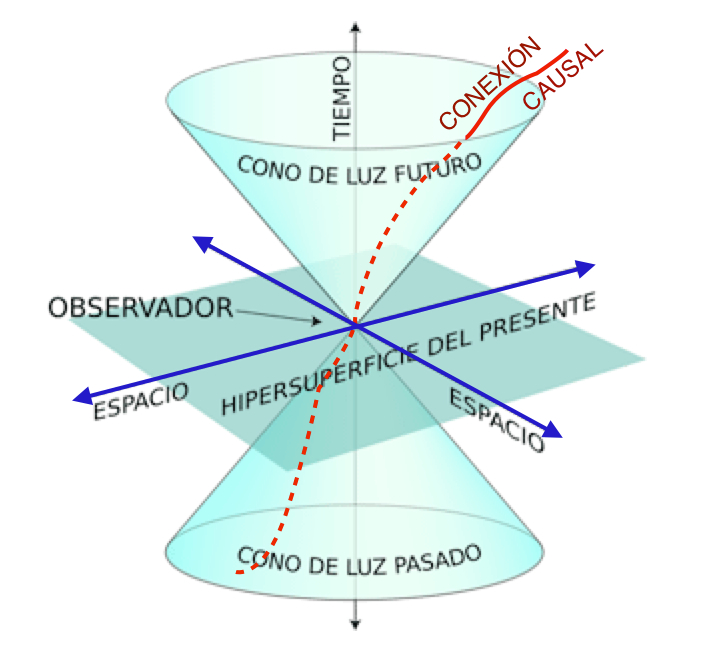
\includegraphics[width=2.6in]{VOLUMEN_1/03_Funciones_Lineales/Figuras/Figura3_3.jpg}
\caption{Cono de luz, espacio-tiempo y eventos.}
\label{Figura3_3}
\end{minipage}
\end{figure}
%%%%%%%%%%%%%%%%%

Construyamos ahora el tipo de transformaci�n de coordenadas que mantiene estos dos supuestos\footnote{Estamos suponiendo que observadores, sistemas de coordenadas y sistemas de referencia son conceptos equivalentes.}:
\begin{enumerate}
\item El producto interno de dos vectores es independiente de la base que expande el espacio vectorial.
 \item Las componentes del tensor m�tricos son invariantes bajo transformaciones de coordenadas.
\end{enumerate}

Si el producto interno de dos vectores es independiente de la base que expanda el espacio vectorial, tendremos:
\[
\left< x \right.  \left|  y \right> =\left< \tilde{x} \right.  \left| \tilde{y}\right> \quad \Leftrightarrow \quad
 x^{\alpha}y_{\alpha}=\tilde{x}^{\alpha}\tilde{y}_{\alpha} \quad \Leftrightarrow \quad  x^{\alpha}y^{\beta}\eta_{\alpha \beta}=\tilde{x}^{\alpha}\tilde{y}^{\beta}\tilde{\eta}_{\alpha \beta}\, ,
\]
y como lo vimos en \ref{TransformaVectoresTensores} las componentes de vectores, bajo cambio de coordenadas, transforman como:
\[
\tilde{a}^{i}=\frac{\partial \tilde{x}^{i}}{\partial x^{k}}\ a^{k} 
\,\, \Rightarrow  \,\,  
 x^{\alpha}y_{\alpha}=\tilde{x}^{\alpha}\tilde{y}_{\alpha} 
 \,\, \Leftrightarrow \,\,  
 x^{\alpha}y^{\beta}\eta_{\alpha \beta}= \frac{\partial \tilde{x}^{\nu}}{\partial x^{\alpha}} x^{\alpha} \frac{\partial \tilde{x}^{\mu}}{\partial x^{\beta}}y^{\beta}\tilde{\eta}_{\nu \mu} = 
 x^{\alpha} y^{\beta} \frac{\partial \tilde{x}^{\nu}}{\partial x^{\alpha}}  \frac{\partial \tilde{x}^{\mu}}{\partial x^{\beta}} \tilde{\eta}_{\nu \mu} \,,
\]
con lo cual concluimos que:
\begin{equation}
\eta_{\alpha \beta}= \frac{\partial \tilde{x}^{\nu}}{\partial x^{\alpha}}  \frac{\partial \tilde{x}^{\mu}}{\partial x^{\beta}} \tilde{\eta}_{\nu \mu} 
\equiv \frac{\partial \tilde{x}^{\nu}}{\partial x^{\alpha}}\frac{\partial\tilde{x}^{\mu}}{\partial x^{\beta}} \eta_{\nu \mu} \,. 
\label{etatransformado}
\end{equation}

Ahora bien, si derivamos (\ref{etatransformado}) respecto a $x^{\gamma}$ tendremos que: 
\[
0 = \eta_{\nu \mu} \left( \frac{\partial^2 \tilde{x}^{\nu}}{\partial x^{\alpha}\partial x^{\gamma}}  \frac{\partial \tilde{x}^{\mu}}{\partial x^{\beta}}  +
\frac{\partial \tilde{x}^{\nu}}{\partial x^{\alpha}}  \frac{\partial^2 \tilde{x}^{\mu}}{\partial x^{\beta}\partial x^{\gamma}} \right) \, .
\]

Como la cantidad dentro del par�ntesis se anula podemos jugar con �sta para descubrir algunas consecuencias ocultas. Es de hacer notar que esa cantidad tiene tres �ndices libres y por lo tanto son 64 ecuaciones que se anulan. Eso significa que le podemos a�adir y sustraer cualesquiera otras con los �ndices intercambiados. 

Supongamos que al par�ntesis anulado le a�adimos una con los �ndices $\alpha$ y $\gamma$ intercambiados y, adicionalmente, le sustraemos una con los �ndices $\gamma$ y $\beta$ intercambiados. Claramente, estamos a�adiendo y sustrayendo ceros.
\[
0 = \eta_{\nu \mu} \left( \frac{\partial^2 \tilde{x}^{\nu}}{\partial x^{\alpha}\partial x^{\gamma}}  \frac{\partial \tilde{x}^{\mu}}{\partial x^{\beta}}  +
\frac{\partial \tilde{x}^{\nu}}{\partial x^{\alpha}}  \frac{\partial^2 \tilde{x}^{\mu}}{\partial x^{\beta}\partial x^{\gamma}} +
 \frac{\partial^2 \tilde{x}^{\nu}}{\partial x^{\gamma}\partial x^{\alpha}}  \frac{\partial \tilde{x}^{\mu}}{\partial x^{\beta}}  +
\frac{\partial \tilde{x}^{\nu}}{\partial x^{\gamma}}  \frac{\partial^2 \tilde{x}^{\mu}}{\partial x^{\beta}\partial x^{\alpha}} -
 \frac{\partial^2 \tilde{x}^{\nu}}{\partial x^{\alpha}\partial x^{\beta}}  \frac{\partial \tilde{x}^{\mu}}{\partial x^{\gamma}}  -
\frac{\partial \tilde{x}^{\nu}}{\partial x^{\alpha}}  \frac{\partial^2 \tilde{x}^{\mu}}{\partial x^{\gamma}\partial x^{\beta}} 
\right) \, .
\] 
Con este truco, vemos que el �ltimo t�rmino anula el segundo y el pen�ltimo el cuarto, de forma y manera que nos queda: 
\[
0 = 2\eta_{\nu \mu}\frac{\partial^2 \tilde{x}^{\nu}}{\partial x^{\alpha}\partial x^{\gamma}}  \frac{\partial \tilde{x}^{\mu}}{\partial x^{\beta}} \,,
\]

Con lo cual la �nica posibilidad que resulta es la siguiente: 
\begin{equation}
0 = \frac{\partial^2 \tilde{x}^{\nu}}{\partial x^{\alpha}\partial x^{\gamma}} 
\,\, \Rightarrow\,\, \tilde{x}^{\nu}=\Lambda^{\nu}_{\mu} x^{\mu} + a^{\nu} \,,
\label{translorentz}
\end{equation}
con: $\Lambda^{\nu}_{\mu}$  y $a^{\nu}$ constantes.

Las transformaciones lineales (\ref{translorentz}) se conocen como \textit{las transformaciones, inhomog�neas, de Lorentz} o tambi�n las transformaciones de Poincar�. Estas transformaciones forman un grupo y, uno de los posibles subgrupos lo constituye el conjunto de transformaciones propias de Lorentz de la forma:
\[
\Lambda^{0}_{0} =1, \quad \Lambda^{i}_{0} = \Lambda^{0}_{j} =0, \quad \mathrm{y} \quad \Lambda^{i}_{j} = R^{i}_{j}  \,,
\]
con: $i, j = 1,2,3$, y donde $R^{i}_{j}$ es una matriz de rotaci�n. 

Supongamos el caso m�s sencillo de este grupo de transformaciones: $a^{\nu} = 0$, en la ecuaci�n (\ref{translorentz}). 
Expl�citamente hemos identificado una transformaci�n de la forma: 
\[
\tilde{x}^{\alpha} = \Lambda^{\alpha}_{0}x^{0} + \Lambda^{\alpha}_{1}x^{1} + \Lambda^{\alpha}_{2}x^{2} +\Lambda^{\alpha}_{3}x^{3} \, ,
\]
la cual, por construcci�n, deja invariante el intervalo tetradimensional:
\[
\mathrm{d}s^{2} = c^2\mathrm{d}t^{2} - \mathrm{d}x^{1} -\mathrm{d}x^{2} - \mathrm{d}x^{3} = \eta_{\mu \nu} \mathrm{d}x^{\mu}{d}x^{\nu} \,, 
\]
con $\eta_{\mu \nu}$ el tensor m�trico. Aqu� $c$ es la constante que representa la velocidad de la luz en el vac�o. Por razones de conveniencia se escoge un sistema de unidades donde $c=1$\footnote{Un sistema de unidades denominado {\it sistema de unidades geometrizado} en el cual la velocidad de la luz y la constante de gravitaci�n universal se toman como la unidad: $c=G=1$.}. 

Es inmediato demostrar que este tipo de transformaciones deja invariante el intervalo. Primero, notemos que: 
\[
\tilde{\eta}^{\mu \nu} = \Lambda^{\mu}_{\alpha}\Lambda^{\nu}_{\beta} \eta^{\alpha \beta} 
\,\, \Rightarrow  \,\,  \eta^{\mu \nu} \eta_{\nu \gamma} = \delta^{\mu}_{\gamma} = \Lambda^{\mu}_{\alpha}\Lambda^{\nu}_{\beta} \eta^{\alpha \beta} \eta_{\nu \gamma} \,\, \Rightarrow  \,\,   
\Lambda^{\mu}_{\alpha}\Lambda_{\gamma}^{\alpha} = \delta^{\mu}_{\gamma}
\]
y como $\mathrm{d}\tilde{x}^{\mu} = \Lambda^{\mu}_{\alpha} \mathrm{d}x^{\alpha}$, entonces: 
\[
\mathrm{d}\tilde{s}^{2} = \tilde{\eta}_{\mu \nu}  \mathrm{d}\tilde{x}^{\mu}\mathrm{d}\tilde{x}^{\nu} \equiv
\eta_{\mu \nu}  \Lambda^{\mu}_{\alpha} \mathrm{d}x^{\alpha}\Lambda^{\nu}_{\beta} \mathrm{d}x^{\beta} =  
\eta_{\alpha \beta}   \mathrm{d}x^{\alpha}\mathrm{d}x^{\beta} = \mathrm{d}s^{2} \,.
\]

Para construir una de las expresiones m�s utilizadas del grupo de Lorentz consideramos la siguiente situaci�n: un observador, $\tilde{x}^{\mu}$, ve moverse una part�cula con una velocidad $\mathbf{v}$, mientras que un segundo observador, $x^{\mu}$, la percibe en reposo.  Entonces, para el observador que registra la part�cula en reposo resulta que $\mathrm{d}x^{i}=0$, y: 
\[
\mathrm{d}\tilde{x}^{\mu} = \Lambda^{\mu}_{\alpha} \mathrm{d}x^{\alpha} \,\, \Rightarrow  \,\,   
\left\{
\begin{array}{ll}
\mathrm{d}\tilde{t}     & =  \Lambda^{0}_{0} \, \mathrm{d}t  \\
    &    \\
  \mathrm{d}\tilde{x}^{i}      & = \Lambda^{i}_{\alpha} \mathrm{d}x^{\alpha} = \Lambda^{i}_{0} \, \mathrm{d}t \qquad \text{con } i = 1,2,3. 
\end{array}\right.
\label{dxtilde2}
\]
Ahora bien, las ecuaciones anteriores nos imponen: 
\[
\mathbf{v} = \frac{\mathrm{d}\tilde{\mathbf{x}}}{\mathrm{d}\tilde{t}} 
\,\, \Rightarrow  \,\,  
v^{i}=\frac{\mathrm{d}\tilde{x}^{i}}{\mathrm{d}\tilde{t}} 
\quad \Rightarrow  \Lambda^{i}_{0} = v^{i}\,\Lambda^{0}_{0} \,.
\]
Adem�s, tenemos que:
\[
\tilde{\eta}_{\alpha \beta} = \Lambda^{\mu}_{\alpha}\Lambda^{\nu}_{\beta} \eta_{\mu \nu}
\,\, \Rightarrow  \,\, 
1 = \Lambda^{\mu}_{0}\Lambda^{\nu}_{0} \eta_{\mu \nu} = 
\left(\Lambda^{0}_{0}\right)^{2} -\left(\Lambda^{1}_{0}\right)^{2} - \left(\Lambda^{2}_{0}\right)^{2} - \left(\Lambda^{3}_{0}\right)^{2} \,, 
\] 
con una soluci�n de la forma:
\[
\Lambda^{0}_{0} = \gamma\,, \quad \Lambda^{i}_{0} = \gamma \, v^{i} \,,
\]
donde:
\[
\gamma = \frac{1}{\sqrt{1 - (\mathbf{v})^2}} \equiv \frac{1}{\sqrt{1 - v^{i}v_{i}} }  \equiv \frac{1}{\sqrt{1 - \left[\left(v^{1}\right)^{2} + \left(v^{2}\right)^{2} +\left(v^{3}\right)^{2}\right]} } \,,
\]
los otros t�rminos $\Lambda^{i}_{j}$ no quedan un�vocamente determinados porque est� de por medio la arbitrariedad de una rotaci�n $R^{i}_{j}$.  Por ello, una selecci�n arbitraria pero razonable de todos los t�rminos $\Lambda^{i}_{j}$ es:
\[
\Lambda^{i}_{j} = \delta^{i}_{j} + v^{i}v_{j} \frac{\gamma -1}{ (\mathbf{v})^2} \equiv  
\delta^{i}_{j} + v^{i}v_{j}\frac{\gamma -1}{ v^{k}v_{k} }\,.
\]
De esta forma quedan determinados todos los elementos de las transformaciones de Lorentz.

Los observadores lorentzianos son los equivalentes a los observadores galileanos en las teor�as newtonianas: son observadores que se mueven uno respecto al otro con una velocidad constante y, desempe�an el mismo papel que los observadores inerciales. Quiz� la consecuencia m�s impactante de la necesidad de vincular mediciones de distintos observadores lorentzianos a trav�s de transformaciones de Lorentz, lo ilustra la evoluci�n distinta del tiempo medido por los diferentes observadores. Un observador en reposo respecto a un reloj, ve avanzar el tiempo con \textit{tic} separados por $\mathrm{d}t = \Delta t$, ya que su reposo respecto al reloj implica:  $\mathrm{d}x^{i}=0$, por lo tanto la separaci�n espacio temporal ser�:
\[
\mathrm{d}s^{2} = \mathrm{d}t^{2} - (\mathrm{d}{x}^i)^{2} =\left(\Delta t \right)^{2} \,\, \Rightarrow  \,\, \mathrm{d}t = \Delta t \,,
\]
mientras que un segundo observador, en movimiento,  tendr� el mismo elemento de l�nea pero expresado como:
\[
\mathrm{d}\tilde{s}^{2} = \mathrm{d}\tilde{t}^{2} - 
(\mathrm{d}{\tilde x}^i)^{2} = \left(1 -\mathbf{v}^{2}\right)  \mathrm{d}\tilde{t} \,\, \Rightarrow  \,\,  
\mathrm{d}\tilde{t} = \frac{\Delta t}{\sqrt{1 -\mathbf{v}^{2}}} \,,
\]
y �sta �ltima ecuaci�n claramente indica que el tiempo evoluciona m�s lento para relojes en movimiento.


\subsection{{\color{Fuchsia}Ejemplos}} 
\label{ejemploslorentz}
\begin{enumerate}
\item  En este ejemplo vamos a repetir, para el caso bidimensional, lo expuesto de manera general en la secci�n anterior. Como vimos, las transformaciones de Lorentz  relacionan las coordenadas del espacio-tiempo medidas por un observador $O$ de un evento, con las coordenadas medidas por otro observador $\tilde{O}$ del mismo evento. El observador $O$ lo representaremos por las coordenadas $\{t,x,y,z\}=\{ {x}^{0}, {x}^{1}, {x}^{2}, {x}^{3}\}$, mientras que el observador $\tilde{O}$ por $\{\tilde{t},\tilde{x},\tilde{y}, \tilde{z}\}=\{ \tilde{x}^{0}, \tilde{x}^{1}, \tilde{x}^{2}, \tilde{x}^{3}\}$. Para lo que sigue, supondremos que cuando los observadores coincidan los relojes de ambos marcar�n $t=t'=0$.

La ecuaci�n (\ref{translorentz}), 
\[
\tilde{x}^{\nu}=\Lambda^{\nu}_{\mu} x^{\mu} \,,
\] 
la podemos expandir en lo que realmente es:
\begin{eqnarray*}
\tilde{t}=\tilde{x}^{0}&=&\Lambda^{0}_{0} x^{0} + 
\Lambda^{0}_{1} x^{1} + \Lambda^{0}_{2} x^{2} + 
\Lambda^{0}_{3} x^{3} \\
\tilde{x}=\tilde{x}^{1}&=&\Lambda^{1}_{0} x^{0} + 
\Lambda^{1}_{1} x^{1} + \Lambda^{1}_{2} x^{2} + 
\Lambda^{1}_{3} x^{3} \\
\tilde{y}=\tilde{x}^{2}&=&\Lambda^{2}_{0} x^{0} + 
\Lambda^{2}_{1} x^{1} + \Lambda^{2}_{2} x^{2} + 
\Lambda^{2}_{3} x^{3} \\
\tilde{z}=\tilde{x}^{3}&=&\Lambda^{3}_{0} x^{0} + 
\Lambda^{3}_{1} x^{1} + \Lambda^{3}_{2} x^{2} + 
\Lambda^{3}_{3} x^{3} 
\end{eqnarray*}

Vamos a suponer que $\tilde{O}$ se mueve respecto a ${O}$, con velocidad $v$, �nicamente en la direcci�n $x$, es decir, $\tilde{y}=y$ y $\tilde{z}=z$. Se supone entonces que $\tilde{t}$ no depender� ni de $y$ ni de $z$ y que cuando $\tilde{x}=0$ entonces ${x}=vt$. 
Todo esto hace que el sistema de ecuaciones anterior se simplifique de manera significativa: 
\begin{eqnarray*}
\tilde{t}=\tilde{x}^{0}&=&\Lambda^{0}_{0} x^{0} +\Lambda^{0}_{1} x^{1} =
\Lambda^{0}_{0} t +\Lambda^{0}_{1} x  \\
\tilde{x}=\tilde{x}^{1}&=&\Lambda^{1}_{1}(x^1-vt)=\Lambda^{1}_{1} (x-vt)\\
\tilde{y}=\tilde{x}^{2}&=& x^{2} = y\\
\tilde{z}=\tilde{x}^{3}&=& x^{3} = z 
\end{eqnarray*}

Debemos determinar los coeficiente $\Lambda^{0}_{0}$, $\Lambda^{0}_{1}$ y $\Lambda^{1}_{1}$. Para tal fin vamos a suponer que cuando $\tilde{t}=t=0$ un pulso de luz es emitido desde el origen de coordenadas. Recordemos que en ese instante ambos observadores coinciden. Como suponemos adem�s que la velocidad de la luz es constante, la onda de luz se propagar� en todas las direcciones de manera que cada observador podr� describirla mediante la ecuaci�n de una esfera cuyo radio aumenta con el tiempo a velocidad $c$. Esto es:
\[
\tilde{x}^2+\tilde{y}^2+\tilde{z}^2=c^2\tilde{t}^2  \quad \mbox{y} \quad
{x}^2+{y}^2+{z}^2=c^2{t}^2 \,.
\]
Por lo tanto:
\[
(\Lambda^{1}_{1} (x-vt))^2+{y}^2+{z}^2=c^2(\Lambda^{0}_{0} t +\Lambda^{0}_{1} x)^2 \,.
\]

Al desarrollar esta �ltima ecuaci�n obtenemos:
\begin{eqnarray*}
\left(\Lambda^{1}_{1}\right)^2\left(x^2-2xvt+v^2t^2\right)+{y}^2+{z}^2&=&c^2\left(\left(\Lambda^{0}_{0}\right)^2 t^2+2\Lambda^{0}_{0}\Lambda^{0}_{1}xt+\left(\Lambda^{0}_{1}\right)^2 x^2 \right) \\
\left(\left(\Lambda^{1}_{1}\right)^2 -c^2\left(\Lambda^{0}_{1}\right)^2 \right)x^2 +{y}^2+{z}^2-2xt\left( \left(\Lambda^{1}_{1}\right)^2 v+c^2 \Lambda^{0}_{0}\Lambda^{0}_{1}   \right)
&=& \left(c^2 \left(\Lambda^{0}_{0}\right)^2 -v^2\left(\Lambda^{1}_{1}\right)^2 \right)t^2 \,.
\end{eqnarray*}
Como ambos observadores registran la misma onda de luz, entonces:
\begin{eqnarray*}
\left(\Lambda^{1}_{1}\right)^2 -c^2\left(\Lambda^{0}_{1}\right)^2 &=&1 \\
\left(\Lambda^{1}_{1}\right)^2 v+c^2 \Lambda^{0}_{0}\Lambda^{0}_{1}&=&0\\
c^2\left(\Lambda^{0}_{0}\right)^2 -v^2\left(\Lambda^{1}_{1}\right)^2&=&c^2 \,.
\end{eqnarray*}

Al resolver este sistema de tres ecuaciones con tres inc�gnitas resulta:
\[
\Lambda^{1}_{1}=\Lambda^{0}_{0}= \frac{1}{\sqrt{1-\frac{v^2}{c^2}}}\,,\quad \Lambda^{0}_{1}=\frac{v}{c^2\sqrt{1-\frac{v^2}{c^2}}} \,.
\]

Si definimos $\gamma=\frac{1}{\sqrt{1-\frac{v^2}{c^2}}}$, las transformaciones de Lorentz quedan entonces de la forma:
\[
\tilde{t}= \left(t -\frac{v}{c^2} x\right) \gamma \,,\quad
\tilde{x}=\left(x-vt\right)\gamma \,,\quad
\tilde{y}= y\,,\quad
\tilde{z}= z \,.
\]

Existen las transformaciones inversas que se pueden obtener de la misma manera que las anteriores.
\[
{t}= \left(\tilde{t} +\frac{v}{c^2} \tilde{x}\right) \gamma \,,\quad
{x}=\left(\tilde{x}+ v \tilde{t}\right)\gamma \,,\quad
{y}=  \tilde{y}\,,\quad
{z}=  \tilde{z}\,.
\]

Notemos que cuando el observador $\tilde{O}$ se mueve a velocidades muy peque�as en comparaci�n a $c$, entonces el factor $\gamma$  tiende a la unidad:
\[
v \ll c \,\, \Rightarrow  \,\,   \gamma \rightarrow 1 \,,
\]
por lo tanto: 
\[
\tilde{t}= t   \,,\quad
\tilde{x}=x-vt \,,\quad
\tilde{y}= y\,,\quad
\tilde{z}= z \,.
\]
que no son m�s que la transformaci�n de Galileo. 

\item  Si un observador $\tilde{O}$ determina que dos eventos ocurren en el mismo lugar, pero  separados en el tiempo; entonces, un observador  ${O}$ �c�mo los apreciar�a? Veamos dos situaciones diferentes. 
\begin{itemize}
\item Consideremos a una persona sentada en un tren en movimiento, observador $\tilde{O}$, esta persona enciende y apaga r�pidamente una linterna dos veces, con una diferencia de 15 minutos entre un evento y el otro. Entonces para $\tilde{O}$ ser� dos eventos que ocurren en el mismo lugar. Pero para el observador ${O}$ que se encuentra en tierra los eventos habr�n ocurrido en lugares diferentes, y esto no parece tener ning�n conflicto con nuestra experiencia e intuici�n. 

\item Si $\tilde{O}$ sigue en su asiento del tren y observa 
que dos personas, uno a cada extremo del vag�n (a unos 30 mts), encienden las linternas al mismo tiempo, entonces para $\tilde{O}$ ser� un evento simult�neo, pero para el observador en tierra ${O}$ que ve al tren alejarse determinar� que la persona de la parte trasera encendi� la linterna un poco antes que la persona apostada en la parte delantera. Esto tal vez si nos resulte algo extra�o. 
\end{itemize}

Consideremos que el tren viaja a $36$ m/s ($\approx 130$ Km/h) entonces,  esta peque�a velocidad se refleja en el factor $\gamma$  de la manera siguiente: 
\[
\frac{v}{c}=1.2\times 10^{-7} \rightarrow  \frac{v^2}{c^2}=1.44\times 10^{-14} \rightarrow \gamma=\frac{1}{\sqrt{1-1.44 \times 10^{-14}} }
\approx 1.000000000000007 \,.
\]

Cuando consideramos la primera situaci�n, la diferencia entre un evento y el otro era de $15$ minutos ($900$ seg), y para el observador en tierra ambos eventos ocurren en dos lugares diferentes: $x_1$ y $x_2$,
\[
{x}_1=\left(\tilde{x}_1+ v \tilde{t}_1\right)\gamma \,,\quad
{x}_2=\left(\tilde{x}_2+ v \tilde{t}_2\right)\gamma \,,
\]
de manera que:
\[
{x}_2-{x}_1=\left(\tilde{x}_2+ v \tilde{t}_2\right)\gamma -\left(\tilde{x}_1+ v \tilde{t}_1\right)\gamma= \left(\tilde{x}_2- \tilde{x}_1\right)\gamma +
\left(\tilde{t}_2- \tilde{t}_1\right)v \gamma \,.
\]

Pero: $\tilde{x}_2=\tilde{x}_1$ y $\tilde{t}_2- \tilde{t}_1=15$ min. Por lo tanto:
\[
{x}_2-{x}_1= (900\ \mbox{s}) (36\ \mbox{m}.\mbox{s}^{-1})\gamma = 32400 \mbox{m}= 32.4 \mbox{Km} \,.
\]

Para la segunda situaci�n, el observador en tierra puede dar fe que los dos eventos ocurren en tiempos diferentes: $t_1$ y $t_2$,
\[
t_1=\left(\tilde{t}_1 +\frac{v}{c^2} \tilde{x}_1\right) \gamma\,,\quad
t_2=\left(\tilde{t}_2 +\frac{v}{c^2} \tilde{x}_2\right) \gamma \,,
\]
de manera que:
\[
t_2-t_1=\left(\tilde{t}_2 +\frac{v}{c^2} \tilde{x}_2\right) \gamma -\left(\tilde{t}_1 +\frac{v}{c^2} \tilde{x}_1\right) \gamma =\left(\tilde{t}_2 -\tilde{t}_1\right) \gamma + \left(\tilde{x}_2 -\tilde{x}_1\right) \frac{v}{c^2} \gamma \,,
\]
con: $\tilde{t}_2 =\tilde{t}_1$ y $\tilde{x}_2 -\tilde{x}_1=30$ metros, resulta:
\[
t_2-t_1=\left(30\ \mbox{m}\right)\left[ \frac{ 36\ \mbox{m}.\mbox{s}^{-1} }{(3\times 10^8 \ \mbox{m}.\mbox{s}^{-1})^2}\right] \gamma= 1.2\times 10^{-14}\ \mbox{s} \,.
\]
\end{enumerate}

Intervalo de tiempo muy peque�o pero diferente de cero: el observador en tierra no aprecia que los eventos fueron simult�neos. 

Este valor tan peque�o, obviamente, es debido a que el factor $\gamma$ es casi la unidad. Notemos que si el tren viajara a una velocidad cercana a $c$, digamos $v=0.99999999 \ c$, entonces:
\[
\frac{v}{c}=0.99999999 \rightarrow  \frac{v^2}{c^2}=0.99999998 \rightarrow \gamma=\frac{1}{\sqrt{1-0.99999998}}
\approx 7071.06780 \,.
\]
por lo que:
\[
t_2-t_1=\left(30\ \mbox{m}\right) \left[\frac{ 36\ \mbox{m}.\mbox{s}^{-1} }{(3\times 10^8 \ \mbox{m}.\mbox{s}^{-1})^2}\right] \gamma= 8.49\times 10^{-11}\ \mbox{s} \,.
\]

En vista de lo anterior, se podr�a esperar que ocurran cosas curiosas con las longitud de los objetos.  Supongamos que el observador que viaja en el tren coloca su laptop en el piso y mide su longitud. Esto significa que la computadora est� en reposo para $\tilde{O}$ y, en la direcci�n del eje $x$, la laptop mide $\tilde{x}_2-\tilde{x}_1$ seg�n $\tilde{O}$. Para el observador que est� en tierra la laptop viaja a una velocidad $vt$, de manera que:
\[
\tilde{x}_2-\tilde{x}_1= \left[({x}_2-{x}_1)-v({t}_2-{t}_1) \right]\gamma\,,
\]

Para el observador que se encuentra en reposo la laptop mide ${x}_2-{x}_1$, medida en el instante ${t}_2={t}_1$. Por lo tanto:
\[
{x}_2-{x}_1=\frac{\tilde{x}_2-\tilde{x}_1}{\gamma}\,.
\]
�La laptop se contrae por el factor $\gamma$!


\newpage
\subsection{{\color{red}Practicando con Maxima}}

\begin{enumerate}
\item En los grandes aceleradores de part�culas se puede producir piones cargados cuando se hace colisionar protones  de gran energ�a con alg�n blanco preparado para este fin. Se conoce que los piones tienen una vida media muy corta: $1.77 \times 10^{-8}$ seg. Lo que esto significa es, que una vez que se producen los piones, la mitad de ellos se habr� desintegrado en un tiempo de $1.77 \times 10^{-8}$ seg. 

Los experimentos en el acelerador reflejan el hecho de que la intensidad del haz de piones que emerge del blanco, y que viaja a $0.99 \ c$, se reduce a la mitad una vez que recorren $37.2$ mts. 
Pero sucede que si los piones viajan a $0.99 \ c= 2.968\times 10^8$ m/s cuando estos hayan deca�do a la mitad la distancia que habr�n recorrido es $d=vt$:

%%%%%% INPUT:
\begin{minipage}[t]{8ex}
{\color{red}\bf \begin{verbatim} (%i1) 
\end{verbatim}}
\end{minipage}
\begin{minipage}[t]{\textwidth}{\color{blue}
\begin{verbatim}
d:(2.968*10^8*(m/s))*(1.77*10^(-8)*s);
\end{verbatim}}
\end{minipage}

%%% OUTPUT:
\begin{math}\displaystyle \parbox{8ex}{\color{labelcolor}(\%o1) }
5.25336\,m
\end{math}
\newline

�Y entonces por qu� el experimento mide que viajaron $37.2$ mts? Bueno, no estamos considerando los efectos relativistas que est�n contenidas en las transformaciones de Lorentz:
\[
t_2-t_1= (\tilde{t}_2-\tilde{t}_1)\gamma \,\, \Rightarrow  \,\,  
\Delta t= \Delta \tilde{t} \gamma \,,
\]
donde $\Delta \tilde{t}$ es el tiempo propio, el tiempo medido por un reloj respecto a la part�cula en movimiento, es decir, el sistema de referencia donde el pion se encuentra en reposo. 

Calculemos, primeramente el factor $\gamma$:

%%%%%% INPUT:
\begin{minipage}[t]{8ex}
{\color{red}\bf \begin{verbatim} (%i2) 
\end{verbatim}}
\end{minipage}
\begin{minipage}[t]{\textwidth}{\color{blue}
\begin{verbatim}
gamma:1/sqrt(1-(0.99)^2);
\end{verbatim}}
\end{minipage}

%%% OUTPUT:
\begin{math}\displaystyle \parbox{8ex}{\color{labelcolor}(\%o2) }
7.088812050083354
\end{math}
\newline

Por lo tanto, la vida media de los piones medida desde el laboratorio es:

%%%%%% INPUT:
\begin{minipage}[t]{8ex}
{\color{red}\bf \begin{verbatim} (%i3) 
\end{verbatim}}
\end{minipage}
\begin{minipage}[t]{\textwidth}{\color{blue}
\begin{verbatim}
Delta_t:(1.77*10^(-8)*s)*gamma;
\end{verbatim}}
\end{minipage}

%%% OUTPUT:
\begin{math}\displaystyle \parbox{8ex}{\color{labelcolor}(\%o3) }
1.254719732864754 \times 10^{-7}\,s
\end{math}
\newline

Seg�n las personas que miden el experimento, y que est�n en el sistema en reposo, los piones viven $\approx 1.255 \times 10^{-7}$ s,  y por lo tanto viajan una distancia: $x=(0.99 c) \Delta t$

%%%%%% INPUT:
\begin{minipage}[t]{8ex}
{\color{red}\bf \begin{verbatim} (%i4) 
\end{verbatim}}
\end{minipage}
\begin{minipage}[t]{\textwidth}{\color{blue}
\begin{verbatim}
(2.968*10^8*(m/s))*Delta_t;
\end{verbatim}}
\end{minipage}

%%% OUTPUT:
\begin{math}\displaystyle \parbox{8ex}{\color{labelcolor}(\%o4) }
37.24008167142589\,m
\end{math}
\newline 

\item Procederemos ahora a resolver con  {\bf Maxima} el sistema que nos condujo a las transformaciones impropias de Lorentz. 

Primero, escribamos una lista que contiene el sistema de ecuaciones:

%%%%%% INPUT:
\begin{minipage}[t]{8ex}
{\color{red}\bf \begin{verbatim} (%i5) 
\end{verbatim}}
\end{minipage}
\begin{minipage}[t]{\textwidth}{\color{blue}
\begin{verbatim}
sis:[L11^2-c^2*L01^2=1,L11^2*v+c^2*L01*L00=0,c^2*L00^2-v^2*L11^2=c^2];
\end{verbatim}}
\end{minipage}

%%% OUTPUT:
\begin{math}\displaystyle \parbox{8ex}{\color{labelcolor}(\%o5) }
\left[ {\tt L_{11}}^2-c^2\,{\tt L_{01}}^2=1 , v\,{\tt L_{11}}^2+c^2
 \,{\tt L_{00}}\,{\tt L_{01}}=0 , c^2\,{\tt L_{00}}^2-v^2\,
 {\tt L_{11}}^2=c^2 \right]
\end{math}
\newline

Es importante agregar la informaci�n de que $v>0$, y que adem�s $v<c$, para evitar soluciones complejas. El comando {\bf assume} nos permite restringir el valor de los par�metros.

%%%%%% INPUT:
\begin{minipage}[t]{8ex}
{\color{red}\bf \begin{verbatim} (%i6) 
\end{verbatim}}
\end{minipage}
\begin{minipage}[t]{\textwidth}{\color{blue}
\begin{verbatim}
assume(v>0,c>v);
\end{verbatim}}
\end{minipage}

%%% OUTPUT:
\begin{math}\displaystyle \parbox{8ex}{\color{labelcolor}(\%o6) }
\left[ v>0 , c>v \right]
\end{math}
\newline

Procedemos a resolver el sistema de ecuaciones, lo podemos hacer con ayuda del comando {\bf solve}:

%%%%%% INPUT:
\begin{minipage}[t]{8ex}
{\color{red}\bf \begin{verbatim} (%i7) 
\end{verbatim}}
\end{minipage}
\begin{minipage}[t]{\textwidth}{\color{blue}
\begin{verbatim}
S:solve(sis,[L11,L00,L01]);
\end{verbatim}}
\end{minipage}

%%% OUTPUT:
\begin{math}\displaystyle \parbox{8ex}{\color{labelcolor}(\%o7) }
\left[ \left[ {\tt L_{11}}=\frac{c}{\sqrt{c^2-v^2}} , {\tt L_{00}}=
 \frac{c}{\sqrt{c^2-v^2}} , {\tt L_{01}}=\frac{\sqrt{c-v}\,v\,\sqrt{v
 +c}}{c\,v^2-c^3} \right]  \right. , \\ 
\quad \quad  \left[\left[ {\tt L_{11}}=\frac{c}{\sqrt{c^2-v
 ^2}} , {\tt L_{00}}=-\frac{c}{\sqrt{c^2-v^2}} , {\tt L_{01}}=-\frac{
 \sqrt{c-v}\,v\,\sqrt{v+c}}{c\,v^2-c^3} \right] \right. , \\ 
 \quad \quad \left[
 \left[  {\tt L_{11}}=-\frac{c}{\sqrt{c^2-v^2}} , {\tt L_{00}}=\frac{c}{
 \sqrt{c^2-v^2}} , {\tt L_{01}}=\frac{\sqrt{c-v}\,v\,\sqrt{v+c}}{c\,v
 ^2-c^3} \right]  \right. , \\ 
\quad \quad  \left[ 
  \left[ {\tt L_{11}}=-\frac{c}{\sqrt{c^2-v^2}} , 
 {\tt L_{00}}=-\frac{c}{\sqrt{c^2-v^2}} , {\it L_{01}}=-\frac{\sqrt{c
 -v}\,v\,\sqrt{v+c}}{c\,v^2-c^3} \right]  \right] 
\end{math}
\newline

Seleccionamos la primera de las listas anteriores y factorizamos con la rutina {\bf factor}:

%%%%%% INPUT:
\begin{minipage}[t]{8ex}
{\color{red}\bf \begin{verbatim} (%i8) 
\end{verbatim}}
\end{minipage}
\begin{minipage}[t]{\textwidth}{\color{blue}
\begin{verbatim}
map(factor,S[1]);
\end{verbatim}}
\end{minipage}

%%% OUTPUT:
\begin{math}\displaystyle \parbox{8ex}{\color{labelcolor}(\%o8) }
\left[ {\tt L_{11}}=\frac{c}{\sqrt{c^2-v^2}} , {\tt L_{00}}=\frac{c
 }{\sqrt{c^2-v^2}} , {\tt L_{01}}=\frac{\sqrt{c-v}\,v}{c\,\left(v-c
 \right)\,\sqrt{v+c}} \right] 
\end{math}

\end{enumerate}


\begin{center}
{\color{red}\rule{15.8cm}{0.4mm}}
\end{center}


\subsection{{\color{OliveGreen}Ejercicios}}
\begin{enumerate}

\item En el espacio euclidiano 3D, y en coordenadas cartesianas, no distinguimos entre vectores y $1-$formas debido a que sus componentes transforman de la misma manera. Demuestre que:
\begin{enumerate}
\item ${\tilde a}^{i}=\Lambda^i_j a^j$  $\,\ \wedge \,\,$
${\tilde b}_{j}=\Lambda^i_j b_i$, son la misma transformaci�n si
la matriz $\Lambda^i_j $ es igual a la transpuesta de su inversa, es decir, si es ortogonal. 

\item Considere dos observadores $O:{x, y} \leftrightarrow {x^{1}, x^{2}}$ y $\tilde{O}:{\tilde{x}, \tilde{y}} \leftrightarrow {\tilde{x}^{1}, \tilde{x}^{2} }$ y sus sistemas de coordenadas asociados. 
\begin{enumerate}
\item Considere la siguiente transformaci�n de coordenadas de Galileo:
\[
\tilde{x}^{1} = V^{1}t + \frac{\sqrt{2}}{2}x^{1} - \frac{\sqrt{2}}{2}x^{2} \qquad \text{y} \qquad 
\tilde{x}^{2} = \frac{\sqrt{2}}{2}x^{1} + \frac{\sqrt{2}}{2}x^{2} \,,
\] 
con $V^{1}$ una constante que representa la velocidad relativa entre  $O-\tilde{O}$, y $t$ al tiempo (par�metro de esta transformaci�n).  

A continuaci�n suponga una part�cula que describe un movimiento respecto a $O$ siguiendo una trayectoria recta, esto es $x^{2} = \alpha x^{1}$, donde $\alpha$ es una constante. Encuentre c�mo lo describir�a el observador $\tilde{O}$ respecto a sus coordenadas (${\tilde{x}^{1}, \tilde{x}^{2} }$).

\item Considere ahora la generalizaci�n de la transformaci�n de coordenadas anterior:
\[
\tilde{x}^{1} = V^{1}t + \frac{\sqrt{2}}{2}x^{1} - \frac{\sqrt{2}}{2}x^{2} \qquad \text{y} \qquad 
\tilde{x}^{2} = V^{2}t +  \frac{\sqrt{2}}{2}x^{1} + \frac{\sqrt{2}}{2}x^{2} \,,
\] 
con $V^{1}$ y $V^{2}$ las componentes de una velocidad relativa entre  $O-\tilde{O}$, y $t$ al tiempo. Muestre que la norma de cualquier vector queda invariante respecto a una transformaci�n de coordenadas como la anterior y encuentre la matriz de transformaci�n.
\end{enumerate}
\end{enumerate}

\item Un acelerador produce part�culas que tienen una vida promedio de $5\mu$s. Estas logran alcanzar  una velocidad de $0.6 c$. 
\begin{enumerate}
\item Un observador que se encuentra en reposo en el laboratorio 
�qu� tiempo de vida media le atribuir� a las part�culas?
\item �Qu� distancia promedio viajan las part�culas en el acelerador? 
\item Si suponemos que existe un observador en reposo con respecto a la part�cula �Qu� distancia se desplazar� �ste observador antes de que la part�cula se desintegre? 
\end{enumerate}

\item  Un elemento de �rea cuadrada se encuentra en reposo para un observador $O$. Encuentre el �rea medida por un observador en movimiento $\tilde{O}$ si �ste lleva una velocidad de $0.85 c$ a lo largo de la diagonal del cuadrado.

\item Consideremos un veh�culo se mueve con una velocidad $V$ con respecto a un observador fijo en tierra $O$, y un pasajero dentro del veh�culo que se mueve con una velocidad $\tilde{v}$ con respecto al veh�culo. Sabemos de los cursos b�sicos que la velocidad del pasajero respecto al observador fijo en tierra es simplemente la suma: $v=\tilde{v}+V$. Nos podemos preguntar sobre la forma en que se suman las velocidades en la teor�a especial de la relatividad, es decir, �C�mo se suman las velocidades si consideramos las transformaciones de Lorentz? 
Demuestre que se suman como:
\[
v=\frac{\tilde{v}+V}{1+\tilde{v}\frac{V}{c^2}} \,.
\]

\item Dado un espacio minkowskiano y un observador $O$ que describe los eventos en el espacio-tiempo respecto a un sistema de coordenadas $\{x^{\alpha} \}$, donde $\alpha = 0,1,2$, y $\eta = \mathrm{diag} [ -1,1,1]$ el tensor m�trico. Considere entonces la siguiente transformaci�n de coordenadas:
\[
\tilde{x}^{0} = \gamma(x^{0} - \beta x^{1})\,, \quad 
\tilde{x}^{1} = \gamma(x^{1} - \beta x^{0}) \quad \text{y} \quad
\tilde{x}^{2} = x^{2}\,, \quad \text{con  } \gamma = \frac{1}{\sqrt{1 - \beta^{2}}}\,. 
\] 
Donde $\beta = v/c$ es la velocidad relativa entre $O$ y $\tilde{O}$.
\begin{enumerate}
\item Otra vez, suponga que una part�cula describe una linea recta respecto a $O$: $x^{2} = \alpha x^{1}$, con $\alpha$ igual a una constante. Encuentre c�mo lo describir�a el otro observador $\tilde{O}$ respecto a sus coordenadas (${\tilde{x}^{0}, \tilde{x}^{1}, \tilde{x}^{2} }$).
  \item Encuentre la expresi�n para la transformaci�n de coordenadas, $  \frac{\partial \tilde{x}^{\alpha}}{\partial x^{\beta}} = \Lambda^{\tilde{\alpha}}_{\beta}$ (transformaci�n de Lorentz) entre estos sistemas relativistas  y muestre como la norma: $x^{\alpha}x_{\alpha} = x^{\alpha}x^{\beta} \eta_{\alpha \beta}$,  de cualquier vector  se conserva.
\end{enumerate}
\item Considere el tensor de Maxwell definido como:
  \[ 
F_{\mu \alpha } = \left(\begin{array}{cccc}
  0        & E^{x}  & E^{y}     & E^{z} \\
  -E^{x} & 0         & -cB^{z} &  cB^{y}  \\
  -E^{y} & cB^{z} & 0          & -cB^{x} \\
  -E^{z} & cB^{y} & cB^{x}  &  0
  \end{array}\right)\,,
 \quad \text{otra vez con: } \quad
\eta_{\mu \nu } = \left(
\begin{array}{cccc}
  -1 & 0 & 0  & 0 \\
  0  & 1 & 0  & 0 \\
  0  & 0 & 1  &  0 \\
  0  & 0 & 0  & 1

  \end{array}\right)\,.
  \]
donde $\textbf{\em E} = (E^{x}, E^{y}, E^{z} )$ y $\mathbf{B} = (B^{x}, B^{y}, B^{z})$ son los campos el�ctricos y magn�ticos (respectivamente), medidos por un observador $O$. 
\begin{enumerate}
  \item Si un observador mide un campo el�ctrico $\textbf{\em E} = E^{x} \mathbf{i}$ y ning�n campo magn�tico �Cu�les campos, $F_{\mu \alpha }$,  medir� otro observador que viaja con una velocidad respecto al primero de  ${\boldsymbol \beta} = v\mathbf{i}$?

\item Muestre que las ecuaciones de Maxwell:
$
\nabla \times \mathbf{B}  -\frac{\partial}{ \partial t}  \textbf{\em E}  = 4 \pi \mathbf{J} \,,$ y $ \nabla \cdot \textbf{\em E}  =   4 \pi \rho   
$  
se pueden expresar como:
\[
\frac{\partial}{ \partial x^{\nu}} F^{\mu \nu} \equiv F^{\mu \nu},_{\nu} =  
4 \pi J^{\mu}\,, \quad \mathrm{donde} \; J^{\mu} = (c\rho, J^{1}, J^{2}, J^{3}) \quad \mathrm{y } \,\, \mathbf{J} = (J^{1}, J^{2}, J^{3}) \,,
\]
\item Considere la identidad de Bianchi de la forma:
\[
\frac{\partial F_{\mu \nu}}{\partial x^{\gamma}} +\frac{\partial F_{\nu \gamma}}{\partial x^{\mu}} +\frac{\partial F_{\gamma \mu}}{\partial x^{\nu}} \equiv
\partial_{\gamma} F_{\mu \nu} + \partial_{\mu} F_{\nu \gamma} + \partial_{\nu} F_{\gamma \mu} \equiv 
F_{\mu \nu \, ,\gamma} + F_{\nu \gamma \, ,\mu} +F_{\gamma \mu \, ,\nu} = 0 \,,
\] y demuestre que las otras dos ecuaciones 
$\nabla \cdot \mathbf{B}  = 0$ y  $ \nabla \times \textbf{\em E}  -\frac{\partial }{ \partial t}  \mathbf{B}  = 0$,   tambi�n est�n contenidas en las expresiones $F^{\mu \nu},_{\nu} =  
4 \pi J^{\mu}\,$

\end{enumerate}


\item El  dual de un tensor $\mathbf{B}$ de rango 2, cuadridimensional, puede ser definido de manera que sus componentes vienen dadas por:
\[
\mathcal{B}^{ij}=\frac{1}{2!} \epsilon^{ijkl}B_{kl}\,.
\]
Muestre que $\mathcal{B}$ transforma como:
\begin{enumerate}
\item Un tensor de rango 2 bajo rotaciones.
\item Un pseudotensor bajo inversiones.
\end{enumerate}

\item Construya $\mathcal{F}^{\mu \alpha}$, el dual del tensor de Maxwell ${F}^{\mu \alpha}$. 
 
\item Demuestre que $c^2 \mathbf{B}^2-\mathbf{E}^2$ es un escalar de Lorentz. 

\item Resuelva los ejercicios anteriores utilizando {\bf Maxima}.

\end{enumerate}
\newpage

\section{Espacios de funciones}
\label{espaciosdefunciones}

Los conceptos de espacios vectoriales discretos que hemos estudiado hasta ahora, finitos o infinitos, se pueden extender a espacios de funciones, en donde los vectores del espacio vectorial y las bases son funciones $\{|{F}_n(x)\rangle\}$. La generalizaci�n de bases discretas a continuas se hace transformando el �ndice de las sumatorias en la variable de una integral, de manera que los �ndices se convierten en variables continuas definidas en intervalos finitos o infinitos. 

Como primer paso para el estudio de estos espacios introduciremos un nuevo objeto matem�tico, que como veremos m�s adelante, es de gran importancia y utilidad. 

\subsection{La funci�n delta de Dirac}
Recordemos que la delta de Kronecker $\delta_{ij}$ que definimos con anterioridad es una cantidad que toma valores discretos: $\delta_{ij}=1$ si $i=j$ y $\delta_{ij}=0$ si $i\neq j$. Es posible construir una extensi�n de este objeto matem�tico para que los �ndices puedan tomar cualquier valor real.
%%%%%%%%%%%%%%%%%
\begin{figure}[h]
\begin{minipage}{7.4cm}
Veamos la siguiente sucesi�n de funciones gaussianas:

\[
\delta_n(x)=\sqrt{\frac{n}{{\pi}}}e^{-n x^2}\,,
\]

tal que:

\[
\int_{-\infty}^{\infty} \delta_n(x)\mathrm{d}x = 1 \,,\,\,  n>0 \,.
\]

A medida que el par�metro $n$ aumenta su valor, la curva gaussiana $\delta_n(x)$ ser� cada vez m�s alta  y m�s angosta, y si $n \rightarrow \infty$ la curva ser� entonces infinitamente m�s alta e infinitamente m�s angosta, pero siempre conservando que el �rea bajo la curva ser� igual a la unidad. 
\end{minipage} \hfill 
\begin{minipage}{8.0cm} 
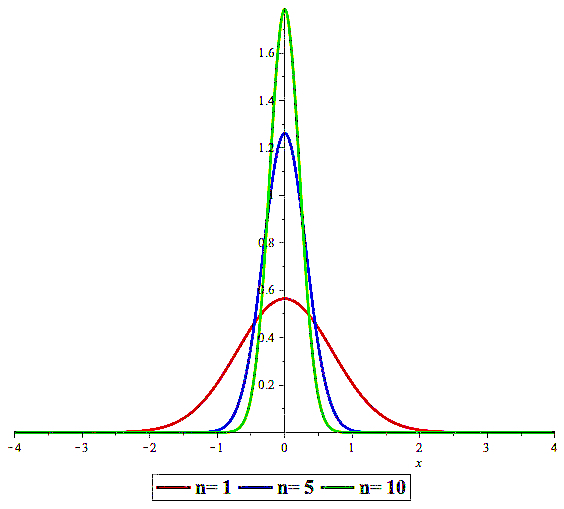
\includegraphics[width=2.6in]{VOLUMEN_1/03_Funciones_Lineales/Figuras/Figura3_4}
\caption{ $\delta_n(x)$ para tres valores diferentes de $n$.}
\end{minipage}
\end{figure}
%%%%%%%%%%%%%%%%%

Esto nos permite definir la ``funci�n'':
\[
\delta(x)=\lim_{n\rightarrow \infty} \sqrt{\frac{n}{{\pi}}}e^{-nx^2}
\,\, \Rightarrow \,\,
\left\{
\begin{array}{lcl}
\delta(x) \rightarrow \infty & \mbox{si} & x \rightarrow 0  \\
& &\\
\delta(x)=0 & \mbox{si} & x \neq 0
\end{array}
\right.
\]

Por tener este comportamiento tan particular no se le suele llamar funci�n, sino una {\it distribuci�n},  y si el punto del m�ximo es un punto diferente de $x=0$, podemos escribir:
\[
\delta(x-x_0)=\lim_{n\rightarrow \infty} \sqrt{\frac{n}{{\pi}}}e^{-n(x-x_0)^2} \,,
\]
donde $x_0$ es el punto donde la gaussiana alcanza su valor m�ximo. 

En general, este proceso de limite puede aplicarse a funciones cuya �rea bajo la curva sea la unidad:
\[
\int_{-\infty}^{\infty} G(x)\mathrm{d}x = 1 \,,
\]
de manera que:
\begin{eqnarray*}
\lim_{n\rightarrow \infty}\int_{-\infty}^{\infty} nG(n(x-x'))f(x')
\mathrm{d}x'&=&
\lim_{n\rightarrow \infty}\int_{-\infty}^{\infty} G(n(x-x'))f\left(x' \right)\mathrm{d}(nx')\\
&=&\lim_{n\rightarrow \infty}\int_{-\infty}^{\infty} G(\tau)f\left(x-\frac{\tau}{n}\right)\ \mathrm{d}\tau=f(x)\,.
\end{eqnarray*}

Si se intercambian los procesos de l�mite e integraci�n:
\[
f(x)= \int_{-\infty}^{\infty}\left[\lim_{n\rightarrow \infty}
nG(n(x-x'))\right]f(x') \mathrm{d}x' \,\, \Rightarrow\,\,
\delta(x-x')=\lim_{n\rightarrow \infty}nG(n(x-x'))\equiv \delta(x,x')\,,
\]
por lo tanto:
\[
f(x)= \int_{-\infty}^{\infty} \delta(x-x')f(x') \mathrm{d}x'\,\, \Rightarrow\,\,
\left\{
\begin{array}{lcl}
\delta(x,x') \rightarrow \infty & \mbox{si} & x \rightarrow x'  \\
& &\\
\delta(x,x')=0 & \mbox{si} & x \neq x'
\end{array}
\right.
\]

La principal propiedad de la delta de Dirac, $\delta(x-x_0)$,  es que:
\[
\int_{-\infty}^{\infty} f(x) \delta(x-x_0) \mathrm{d}x= f(x_0) \,,
\]
es decir, act�a parecido a como lo hace la delta de Kronecker cuando se contrae uno de sus �ndices con las componentes de un vector: $a_j=\delta_j^i a_i$, en el sentido que de todos lo valores selecciona s�lo uno. Adem�s, si $f(x)=1$ entonces: 
\[
\int_{-\infty}^{\infty}  \delta(x-x_0) \mathrm{d}x= 1\,. 
\]

Existen algunas representaciones integrales basadas en el hecho de que $\delta(x-x_0)$ �nicamente existe en $x=x_0$, por ejemplo:
\begin{eqnarray*}
\int_{-\infty}^{\infty}  f(x)\delta(x-x_0) \mathrm{d}x &=& 
\int_{x=x_0-\varepsilon}^{x=x_0+\varepsilon}   f(x)\delta(x-x_0)\mathrm{d}x \,, \\
\int_{a}^{b}  f(x)\delta(x-x_0) \mathrm{d}x &=& 
\left\{
\begin{array}{lcl}
f(x_0) & \mbox{si} & a\leq x_0 \leq b  \\
& &\\
0 & \mbox{si} & x_0 <a \,\,\, \mbox{�}\,\,\, x_0 >b 
\end{array}
\right.
\end{eqnarray*}
Y la funci�n escal�n de Heaviside:  
\[
H(x-x_0)=\int_{-\infty}^{x} \delta(x-x_0) \mathrm{d}x=
\left\{
\begin{array}{lcl}
1 & \mbox{si} & x\geq  x_0   \\
& &\\
0 & \mbox{si} &  x\leq  x_0 
\end{array}
\right. \,\, \Rightarrow\,\,
\delta(x-x_0)=\frac{\mathrm{d}H(x-x_0)}{\mathrm{d}x}\,.
\]

Algunas de las tantas propiedades de la delta de Dirac son las siguientes:
\begin{center}
\begin{tabular}{ll}
$\bullet $ $\delta(x-x_0)=\delta(x_0-x)$ & 
$\bullet $ $\delta(ax)=\frac{\delta(x)}{|a|}$ \\
& \\
$\bullet $ $x\delta(x)=0$ & 
$\bullet $ $f(x)\delta(x-x_0)=f(x_0)\delta(x-x_0)$ \\
& \\
$\bullet $ $\delta(x^2-a^2)=\frac{1}{2|a|}\left[\delta(x-a)+\delta(x+a)\right]$ & 
$\bullet $ $x^{n+1} \frac{\mathrm{d}^n\delta(x)}{\mathrm{d}x^n}=0$\\
& \\
$\bullet $ $\delta({\bf r}-{\bf r}_0)=\delta(x-x_0)\delta(y-y_0)\delta(z-z_0)$ & 
$\bullet $ $\int f({\bf r}) \delta({\bf r}-{\bf r}_0)\mathrm{d}V=f({\bf r}_0)$
\end{tabular}
\end{center}

\subsection{Bases continuas}
Tal y como vimos anteriormente, la representaci�n de un vector $|{a}\rangle$ en un espacio
vectorial abstracto $\textbf{\em V}$ puede darse en t�rmino de una base
ortonormal de vectores 
(discreta y finita $B_{DF} = \left\{  \left|  \mathrm{e}_{1}\right>, \left|  \mathrm{e}_{2}\right>, \left|\mathrm{e}_{3} \right>, \cdots \left|  \mathrm{e}_{n}\right> \right\}  $ o discreta e infinita $B_{DI}=\left\{  \left|  \mathrm{e}_{1}\right>, \left|  \mathrm{e}_{2}\right>, \left|\mathrm{e}_{3} \right> \cdots \left|  \mathrm{e}_{n}\right> \cdots\right\}  $) de la forma:
\[
|{a}\rangle=
\left\{
\begin{array} [c]{l}
c^{i}\ \left|  \mathrm{e}_{i}\right> =
\left< \mathrm{e}^{i}\right|  \left.  {a}\right> \ \left|  \mathrm{e}_{i}\right> 
\,\, \Leftarrow \,\ B_{DF}=\left\{  \left|  \mathrm{e}_{1}\right> ,\ \left|  \mathrm{e}_{2}\right> ,\ \left| \mathrm{e}_{3}\right> \cdots\left|  \mathrm{e}_{n}\right> \right\} \\ \\
c^{i}\ \left|  \mathrm{e}_{i}\right>  =\left< \mathrm{e}^{i}\right|  \left.  {a}\right \rangle \ \left| \mathrm{e}_{i}\right> \,\, \Leftarrow \,\, 
B_{DI}=\left\{  \left|  \mathrm{e}_{1}\right> ,\ \left|  \mathrm{e}_{2}\right> , \left| \mathrm{e}_{3} \right> \cdots \left|  \mathrm{e}_{n} \right> \cdots\right\}
\end{array}
\right.
\]
donde en ambos casos:
\[
c^{i}=\left< \mathrm{e}^{i}\right|  \left.  {a}\right> = c^{j}\ \left< \mathrm{e}^{i}\right.  \left|  \mathrm{e}_{j}
\right> =c^{j}\ \delta_{j}^{i}\,.
\]

Recapitulemos ahora algunos puntos que hemos tratado con anterioridad, y con el fin de aclarar conceptos, para el caso de bases discretas de funciones $\{\left|\mathrm{e}_i(x)\right>\}$.

La relaci�n de ortogonalidad viene dada, como hemos mencionado, por:
\[
\langle{\mathrm{e}^n(x)}|{\mathrm{e}_m(x)}\rangle=\int_{a}^{b}e^{*}_{n}(x)e_{m}(x)\mathrm{d}x=\Theta_n\delta^n_{m} \,,
\]
y con una norma definida como:
\[
\left\|  \left|\mathrm{e}_i(x)\right> \right\|^{2}=
\langle{\mathrm{e}_n(x)}|{\mathrm{e}_n(x)}\rangle=
\int_{a}^{b}\left|e_{n}(x)\right|^2 \mathrm{d}x=\Theta_n \,.
\]
La base ser� ortonormal si $\Theta_n=1$. 

Con una base $\{\left|\mathrm{e}_i(x)\right>\}$ definida, es posible representar cualquier funci�n $\left|f(x)\right>$ cuadrado integrable, es decir que cumpla con:
\[
\int_{a}^{b}\left|f(x)\right|^2 \mathrm{d}x \neq \infty \,,
\]
en una combinaci�n lineal de la base dada:
\[
\left|f(x)\right>= C^i\left|\mathrm{e}_i(x)\right>
\]

Las cantidades $C^i$, las componentes de $\left|f(x)\right>$, se obtienen de la siguiente manera:
\[
\left< \mathrm{e}^{i}(x) \right|\left. f(x)\right>=
 C^j\left< \mathrm{e}^{i}(x) \right|\left. \mathrm{e}_j(x)   \right>=
 C^j \delta^i_{j}=C^i=
\int_{a}^{b} f(x) e^{*}_{i}(x) \mathrm{d}x  \,,
\]

Resulta conveniente para los c�lculos que vienen a continuaci�n cambiar 
$i \rightarrow n$ y $x\rightarrow x'$, de manera que: 
\[
C^n=\int_{a}^{b} f(x') e^{*}_{n}(x') \mathrm{d}x'\,.
\]

Por lo tanto:
\begin{eqnarray*}
\left|f(x)\right>= C^n\left|\mathrm{e}_n(x)\right> \,\, \Rightarrow \,\, 
\left|f(x)\right>&=& \sum_{n}\left[\int_{a}^{b} f(x') e^{*}_{n}(x') \mathrm{d}x' \right]\left|\mathrm{e}_n(x)\right>= \sum_{n} \int_{a}^{b} f(x') e^{*}_{n}(x')\mathrm{e}_n(x) \mathrm{d}x'\\
&=&  \int_{a}^{b} f(x') \sum_{n} e^{*}_{n}(x')\mathrm{e}_n(x) \mathrm{d}x' \,.
\end{eqnarray*}
Utilizando la delta de Dirac:
\[
\left|f(x)\right>=  \int_{a}^{b} f(x') \delta(x-x')\mathrm{d}x'= 
\int_{a}^{b} f(x') \left[ \sum_{n} e^{*}_{n}(x')\mathrm{e}_n(x) \right]\mathrm{d}x'
\,\, \Rightarrow \,\, \delta(x-x')=  \sum_{n} e^{*}_{n}(x')\mathrm{e}_n(x)\,.
\]

Esta �ltima relaci�n viene a ser una generalizaci�n de la relaci�n de cierre mencionada en la secci�n \ref{OrtogonalidadBases}, y se conoce como {\it condici�n de completitud} para la base  $\{\left|\mathrm{e}_i(x)\right>\}$, adem�s,  tambi�n resulta ser una representaci�n en serie para la delta de Dirac.

De todo esto surgen algunas propiedades fundamentales:

\begin{itemize}
\item Se dice que el conjunto $\{\left|\mathrm{e}_i(x)\right>\}$ es {\it completo} si para $\left|f(x)\right>= C^i\left|\mathrm{e}_i(x)\right>$, entonces se tiene que: 
\[  
\int_{a}^{b} \left| f(x)\right|^2=\sum_{n}  \left| C^n\right|^2 \,.
\]
\item Si $\left|f(x)\right>= C^i\left|\mathrm{e}_i(x)\right> $ y 
$ \left| g(x)\right>= E^i\left|\mathrm{e}_i(x)\right>$, entonces $\langle{f(x)}|{g(x)}\rangle= C_n^{*} E^n$.
\end{itemize}

Es posible pasar de estos espacios vectoriales discretos, donde las bases son un conjunto numerable de elementos $\{\mathrm{e}_{n}(x)\}$, a espacios vectoriales de funciones con las bases  dadas por funciones y donde el �ndice $n$ pasa a ser una variable continua. 

Recordemos que en la secci�n \ref{OrtogonalidadBases}  habl�bamos de un conjunto de funciones $\left\{  \left|  \mathrm{e}_{1}\right>, \left|  \mathrm{e}_{2}\right>, \left|  \mathrm{e}_{3}\right>, \cdots ,\left|  \mathrm{e}_{n}\right> \cdots\right\}$ definidas por:
\[
\left|  \mathrm{e}_{0}\right> =1,\quad\left|  \mathrm{e}_{2n-1} \right> =\cos(nx)\quad\text{y}\quad\left|  \mathrm{e}_{2n}\right>= \operatorname{sen}(nx),\quad\text{con } n=1,2,3,\cdots \,,
\]
la base discreta de Fourier. Base que tambi�n podemos escribir de la forma compleja, como se muestra a continuaci�n:
\[
\left|  \mathrm{e}_{n}(x)\right>= \frac{1}{\sqrt{2L}}e^{i\frac{n\pi}{L}x}= 
\frac{1}{\sqrt{2L}}e^{i k x} \,,\quad
\mbox{con  } n=-\infty\dots \infty \,\, \mbox{y} \,\, -L\leq x\leq L\,.
\]

Cuando $n$ aumenta indefinidamente, tambi�n lo har� la cantidad $k=\frac{n\pi}{L}$,  convirti�ndose entonces en una variable continua, es decir, $\Delta k=\frac{\Delta n\pi}{L}\rightarrow 0$. Notemos que los �ndices de la delta de Kronecker $\delta_{nm}=\delta_{nn'}$ pueden tomar los valores: $n=\frac{Lk}{\pi}, n'=\frac{Lk'}{\pi}$, y en el proceso de  $L \rightarrow \infty$ se convertir�n en: 
\[
\delta_{nn'} \,\,\rightarrow \,\,\delta\left(\frac{Lk}{\pi} - \frac{Lk'}{\pi}\right) =
\delta\left(\frac{L}{\pi}( k- k')\right)  = \frac{\pi}{L}\delta\left( k- k' \right)\,.
\]

De esta manera, la base ortonormal quedar� escrita en funci�n de las variables continuas $k$ y $x$, como se muestra a continuaci�n: 
\[
\left|  \mathrm{e}(k,x)\right>= \frac{1}{\sqrt{2\pi}}e^{i k x}\,.
\]

El hecho de que sean ortonormales se refleja en la siguiente condici�n  (que es una extensi�n de la expresi�n para el producto interno de bases discretas) 
\[
\langle \mathrm{e}(k,x) | \mathrm{e}(k,x)\rangle=
\int_a^b  \mathrm{e}(k,x)^{\ast} \mathrm{e}(k',x)\  \mathrm{d}x=\delta(k-k') \,,\quad
\mbox{con } \quad \alpha \leq k \leq \beta \,,\,\, a \leq x \leq b
\] 

Al ser el conjunto de funciones $\{\left|  \mathrm{e}(k,x)\right>\}$ una base, toda funci�n del mismo espacio vectorial se puede expandir en esa base como:
\[
\left| f(x)\right>=\int_\alpha^\beta \mathrm{C}(k) \mathrm{e}(k,x)\mathrm{d}k \,.
\]

En correspondencia con el caso de las bases discretas, el coeficiente $\mathrm{C}(k)$ viene a ser algo parecido a las componentes de $ \left| f(x)\right>$. Y para calcularlas se procede como se muestra a continuaci�n:
\[
 \left<\mathrm{e}(k',x)\right.\left|f(x)\right>=
\int_a^b \mathrm{e}(k',x)^{\ast} f(x)\ \mathrm{d}x =
\int_\alpha^\beta \mathrm{C}(k) \left[ \int_a^b  \mathrm{e}(k',x)^{\ast}  \mathrm{e}(k,x)\   \mathrm{d}x \right] \mathrm{d}k =
\int_\alpha^\beta \mathrm{C}(k) \delta(k-k') \mathrm{d}k = \mathrm{C}(k')\,.
\]

Volvamos a cambiar la notaci�n para los �ndices: $k' \rightarrow k$, $x \rightarrow x'$ en la �ltima ecuaci�n:
\[
\mathrm{C}(k)=\int_a^b \mathrm{e}(k,x')^{\ast} f(x') \mathrm{d}x' \,,
\]
por lo tanto:
\[
\left| f(x)\right>=\int_\alpha^\beta \mathrm{C}(k) \left|  \mathrm{e}(k,x)\right> \mathrm{d}k = \int_a^b f(x') \left[\int_\alpha^\beta \mathrm{e}(k,x')^{\ast}\mathrm{e}(k,x)  \mathrm{d}k\right] \mathrm{d}x' =
 \int_a^b f(x') \delta(x-x') \mathrm{d}x' \,,
\]
y la relaci�n: 
\[
\int_\alpha^\beta \mathrm{e}(k,x')^{\ast}\mathrm{e}(k,x)  \mathrm{d}k=\delta(x-x') \,,
\]
ser� la relaci�n de cierre para el conjunto no numerable de funciones ortonormales. 

Una integral como la que nos permiti� definir $\mathrm{C}(k)$, digamos, del tipo:
\[
F(k)=\int_a^b f(x') \mathrm{e}(k,x')^{\ast}  \mathrm{d}x' 
\quad \Rightarrow 
\left| f(x)\right>=\int_\alpha^\beta F(k) \mathrm{e}(k,x) \mathrm{d}k \,,
\]
es lo que se denomina una transformada de $f(x)$. M�s adelante veremos que si la base, es por ejemplo $e^{ikx}/\sqrt{2\pi}$, la transformada ser� la de Fourier.

En el espacio vectorial de funciones de cuadrado integrable $\mathcal{L}^{2}$, definidas en $\mathds{R}^{3}$, tendremos que:
\[
\left|  {F}\right> =c^{i}\ \left|  \mathrm{e}_{i}\right>  \equiv 
\left< \mathrm{e}^{i}\right|  \left.  {F}\right>\ \left|  \mathrm{e}_{i}\right> =\sum_{i=0}^{\infty}\left( \int_{-\infty}^{\infty}\mathrm{d}^{3}r^{\prime} \xi_{i}^{\ast}\left( \mathbf{r}^{\prime}\right)  \ f\left(  \mathbf{r}^{\prime}\right)  \right) \left|  \mathrm{e}_{i}\right>\,,
\]
que se reescribe en t�rminos de funciones como:
\[
f\left(  \mathbf{r}\right)  =\sum_{i=0}^{\infty}\left(  \int_{-\infty}^{\infty}\mathrm{d}^{3}r^{\prime}\xi_{i}^{\ast}\left(  \mathbf{r}^{\prime}\right)  \ f\left(  \mathbf{r}^{\prime}\right)  \right)  \xi_{i}\left(
\mathbf{r}\right) \,.
\]

Es claro que se pueden intercambiar los s�mbolos de $\int$ y $\sum$, por lo cual:
\[
f\left(  \mathbf{r}\right)  =\int_{-\infty}^{\infty}\mathrm{d}^{3}r^{\prime}\ f\left(  \mathbf{r}^{\prime}\right)  \underset{\mathcal{G}(\mathbf{r}^{\prime},\mathbf{r})}{\underbrace{\left[  \sum_{i=0}^{\infty}\xi_{i}^{\ast}\left(  \mathbf{r}^{\prime}\right)  \xi_{i}\left(  \mathbf{r}\right)\right]  }} \,,
\]
la funci�n $\mathcal{G}(\mathbf{r}^{\prime},\mathbf{r})$, que depende de los argumentos $\mathbf{r}^{\prime}$ y $\mathbf{r}$, vive dentro de las integrales y convierte:
\[
f\left(  \mathbf{r}\right)  =\int_{-\infty}^{\infty}\mathrm{d}^{3}r^{\prime}\ f\left(  \mathbf{r}^{\prime}\right)  \ \mathcal{G}(\mathbf{r}^{\prime },\mathbf{r}) \,.
\]
Podemos ver entonces que:
\[
f\left(  \mathbf{r}\right)  =\int_{-\infty}^{\infty}\mathrm{d}^{3}r^{\prime
}\ f\left(  \mathbf{r}^{\prime}\right)  \ \mathbf{\delta}(\mathbf{r}^{\prime}-\mathbf{r}) \,.
\]

En resumen, la generalizaci�n de bases discretas a continuas se hace transformando el �ndice de la sumatoria en la variable de una integral:
\[
\left| {\Psi}\right> =\int\mathrm{d}\alpha\ c\left(\alpha\right)  \ \left|  {w}_{\alpha}\right> 
\,\, \Rightarrow \,\,
c\left(  \beta\right)  =\left< {w}_{\beta}\right.  \left|{\Psi}\right> =\int\mathrm{d}\alpha\ c\left(  \alpha\right)\ \left< {w}_{\beta}\right.  \left|  {w}_{\alpha}\right> =\int\mathrm{d}\alpha\ c\left(  \alpha\right)  \ \delta\left(\alpha-\beta\right) \,.
\]

As�, para los conceptos expresados hasta ahora se tiene el siguiente tabla resumen:

\begin{center}
\begin{tabular}
[c]{|c|c|c|}\hline
\textbf{Propiedad$\backslash$Base} & \textbf{Discreta} & \textbf{Continua}\\\hline
\textsf{Ortogonalidad} & $\left< {u}^{i}\right.  \left|
{u}_{j}\right> =\delta_{j}^{i}$ & $\ \left< {w}
_{\beta}\right.  \left|  {w}_{\alpha}\right> =\delta\left(
\alpha-\beta\right)  $\\\hline
\textsf{Cierre} & ${1=}\sum_{j=0}^{\infty}\ \left|  {u}
_{j}\right> \left< {u}^{j}\right|  $ & ${1=}
\int\mathrm{d}\alpha\ \left|  {w}_{\alpha}\right> \left<
{w}_{\alpha}\right|  $\\\hline
\textsf{Expansi�n } & $\left|  {F}\right> =\sum_{i=0}
^{\infty}c^{i}\ \left|  {u}_{i}\right> $ & $\left|  {\Psi
}\right> =\int\mathrm{d}\alpha\ c\left(  \alpha\right)  \ \left|
{w}_{\alpha}\right> $\\\hline
\textsf{Componentes} & $c^{i}=\left< {u}^{i}\right|  \left.
{F}\right> $ & $c\left(  \beta\right)  =\left<
{w}_{\beta}\right.  \left|  {\Psi}\right> $\\\hline
\textsf{Producto Interno} & $\left< {G}\right|  \left.
{F}\right> =\sum_{i=0}^{\infty}\ g^{i\ast}\ f_{i}$ &
$\left< {G}\right|  \left.  {F}\right>
=\int\mathrm{d}\alpha\ g^{\ast}\left(  \alpha\right)  \ f\left(
\alpha\right)  $\\\hline
\textsf{Norma} & $\left< {F}\right|  \left.  {F}
\right> =\sum_{i=0}^{\infty}\ \left|  f_{i}\right|  ^{2}$ &
$\left< {F}\right|  \left.  {F}\right>
=\int\mathrm{d}\alpha\ \left|  f\left(  \alpha\right)  \right|  ^{2}$\\\hline
\end{tabular}
\end{center}

\subsection{Bases de ondas planas y la transformada de Fourier}

En las teor�as de oscilaciones es de gran importancia considerar el problema de la transformada de Fourier. Recientemente vimos que una funci�n $f(x)$ puede representarse de la forma:
\[
\left| f(x)\right>=\int_\alpha^\beta \mathrm{C}(k) \mathrm{e}(k,x) \mathrm{d}k\,,
\]
si la funci�n $f(x)$ est� definida en $(-\infty, \infty)$ y si tomamos al conjunto de vectores base al conjunto de funciones continuas y ortonormales $\{\mathrm{e}(k,x)\}$ como $\{\mathrm{e}^{ikx}/\sqrt{2\pi}\}$, entonces la integral anterior la podemos escribir de la forma:
\begin{equation}
\left| f(x)\right>=\frac{1}{\sqrt{2\pi}}\int_{-\infty}^\infty \mathrm{F}(k) \mathrm{e}^{ikx}\ \mathrm{d}k\,,
\label{fxdirecta}
\end{equation}

Si utilizamos la relaci�n de ortogonalidad: 
$\langle \mathrm{e}(k,x) | \mathrm{e}(k,x)\rangle=
\int  \mathrm{e}(k,x) \mathrm{e}(k',x)^{\ast}\  \mathrm{d}x=\delta(k-k')$, resulta:
\[
\int_{-\infty}^\infty \mathrm{e}^{i(k-k')x}\ \mathrm{d}x=2\pi\delta(k-k')\,.
\]
Donde:
\[
\left|\mathrm{F}(k)\right>=\frac{1}{\sqrt{2\pi}}\int_{-\infty}^\infty f(x) \mathrm{e}^{-ikx}\ \mathrm{d}x\,.
\]

A las variables $x$ y $k$ se les denominan variables conjugadas de Fourier (no conjugadas como en variable compleja) y a $\mathrm{F}(k)$ la transformada de Fourier de $f(x)$ (y viceversa).

Notemos que si sustituimos $\mathrm{F}(k)$ en la otra integral, ecuaci�n  (\ref{fxdirecta}), entonces:
\[
\frac{1}{{2\pi}}\int_{-\infty}^\infty \int_{-\infty}^\infty 
f(x) \mathrm{e}^{ik\left(x-x'\right)}\ \mathrm{d}k \ \mathrm{d}x' \,\, \Rightarrow  \,\,  
\left| f(x')\right>=\int_{-\infty}^\infty  f(x) \delta(x-x') \ \mathrm{d}x' \,.
\]

Por otra parte, podemos ver que la integral para $\mathrm{F}(k)$ se puede hacer en dos partes:
\[
\left|\mathrm{F}(k)\right>=\frac{1}{\sqrt{2\pi}}\int_{-\infty}^\infty f(x) \mathrm{e}^{-ikx}\ \mathrm{d}x 
\,\, \Rightarrow  \,\,
\frac{1}{\sqrt{2\pi}}\int_{-\infty}^0 f(x) \mathrm{e}^{-ikx}\ \mathrm{d}x + \frac{1}{\sqrt{2\pi}}\int_{0}^\infty f(x) \mathrm{e}^{-ikx}\ \mathrm{d}x \,.
\]

Si sustituimos  $x\rightarrow-x$, en la primera integral de la ecuaci�n anterior resulta: 
\[
\left|\mathrm{F}(k)\right>=
\frac{1}{\sqrt{2\pi}}\int_{0}^\infty f(-x) \mathrm{e}^{ikx}\ \mathrm{d}x + \frac{1}{\sqrt{2\pi}}\int_{0}^\infty f(x) \mathrm{e}^{-ikx}\ \mathrm{d}x \,.
\]

Dos casos podemos considerar:
\begin{itemize}
\item Si la funci�n es par, $f(x)=f(-x)$:
\[
\left|\mathrm{F}(k)\right>=
\frac{1}{\sqrt{2\pi}}\left[\int_{0}^\infty f(x) \mathrm{e}^{ikx}\ \mathrm{d}x +\int_{0}^\infty f(x) \mathrm{e}^{-ikx}\ \mathrm{d}x\right]=\sqrt{\frac{2}{\pi}}\int_{0}^\infty f(x) \cos(kx)\ \mathrm{d}x \,,
\]
entonces, de la transformada al hacer $\mathrm{F}(k)=\mathrm{F}(-k)$ se tiene:
\[
\left| f(x)\right>=\sqrt{\frac{2}{\pi}}\int_{0}^\infty \mathrm{F}(k) \cos(kx)\ \mathrm{d}k\,.
\]
Estas dos funciones se conocen como las transformadas coseno de Fourier. 

\item Si la funci�n es impar, $f(x)=-f(-x)$:
\[
\left|\mathrm{F}(k)\right>=\frac{1}{\sqrt{2\pi}}\left[\int_{0}^\infty f(-x) \mathrm{e}^{ikx}\ \mathrm{d}x -\int_{0}^\infty f(-x) \mathrm{e}^{-ikx}\ \mathrm{d}x\right]=i\sqrt{\frac{2}{\pi}}\int_{0}^\infty f(x) \mbox{sen}(kx)\ \mathrm{d}x \,.
\]

Ahora al hacer $\mathrm{F}(k)=-\mathrm{F}(-k)$ se tiene: 
\[
\left| f(x)\right>=\sqrt{\frac{2}{\pi}}\int_{0}^\infty \mathrm{\tilde F}(k)  \mbox{sen}(kx)\ \mathrm{d}k\,, 
\]
donde ${\tilde F}(k)=i{F}(k)$. Tenemos ahora las transformadas seno de Fourier.
\end{itemize}

La generalizaci�n a $ \mathds{R}^n$ es obvia. Si $f=f({\bf r})$, entonces: 
\[
\left| f({\bf {r}})\right>=\left[\frac{1}{\sqrt{2\pi}}\right]^{\frac1n}\int_{-\infty}^\infty \cdots  \int_{-\infty}^\infty \mathrm{F}({\bf {k}}) \mathrm{e}^{i({\bf k}\cdot {\bf r})}\ \mathrm{d}{\bf {k}}\,,
\]
donde $\mathrm{d}{\bf {k}}=\mathrm{d}{ {k}}_1\mathrm{d}{ {k}}_2\mathrm{d}{ {k}}_3\dots \mathrm{d}{ {k}}_n$. Para la transformada:
\[
\left|\mathrm{F}({\bf k})\right>=\left[\frac{1}{\sqrt{2\pi}}\right]^{\frac1n}
\int_{-\infty}^\infty \cdots  \int_{-\infty}^\infty f({\bf r})
\mathrm{e}^{-i({\bf k}\cdot {\bf r})}\ \mathrm{d}{\bf {r}}\,,
\]
donde $\mathrm{d}{\bf {r}}=\mathrm{d}{ {x}}_1\mathrm{d}{ {x}}_2\mathrm{d}{ {x}}_3\dots \mathrm{d}{ {x}}_n$, representa el elemento de volumen en $ \mathds{R}^n$.

\subsubsection{Ondas planas}

Como un ejemplo de lo anterior, consideraremos la base de las ondas planas. 
Si a $k$ la llamaremos $s$ y a la variable $x$ el tiempo $t$,  vale decir:
\[
F(s)=\frac{1}{\sqrt{2\pi}}{\displaystyle\int_{-\infty}^{\infty}}
\mathrm{d}t\ {\large e}^{i st}\ f(t) \quad\rightleftarrows\quad f(t)=
\frac{1}{\sqrt{2\pi}}{\displaystyle\int_{-\infty}^{\infty}}\mathrm{d}s\ {\large e}^{-i st}\ F(s) \,.
\]

De esta manera, a la funci�n $F(s)$ se le denomina la distribuci�n espectral de $f(t)$ y a $|F(s)|^2$ la densidad espectral, es decir, la intensidad de la onda en el intervalo $[s,s+\Delta s]$. Esto significa que la energ�a total es:
\[
E=\int_{-\infty}^\infty |F(s)|^2\mathrm{d}s\,.
\]


Tambi�n podemos reescribir las transformadas en t�rminos de la posici�n y el momento:
\[
\psi\left(  x\right)  =\frac{1}{\sqrt{2\pi\hbar}}{\displaystyle\int_{-\infty}^{\infty}}
\mathrm{d}p\ {\large e}^{i({px}/{\hbar})}\ \bar{\psi}\left(  p\right)\quad\rightleftarrows\quad\bar{\psi}\left(  p\right)  =\frac{1}{\sqrt{2\pi\hbar}}{\displaystyle\int_{-\infty}^{\infty}}
\mathrm{d}x\ {\large e}^{-i({px}/{\hbar})}\ \psi\left(  x\right) \,.
\]

Hemos tenido cuidado de incluir los factores de normalizaci�n adecuados para el caso de las descripciones en Mec�nica Cu�ntica. Estas f�rmulas pueden ser reinterpretadas en funci�n de los conceptos anteriormente expuestos y podemos definir una base continua de la forma:
\[
\psi\left(  x\right)  =\frac{1}{\sqrt{2\pi\hbar}}
{\displaystyle\int_{-\infty}^{\infty}}\mathrm{d}p\ \underset{v_{p}\left(  x\right)  }{\underbrace{\left(  \frac
{1}{\sqrt{2\pi\hbar}}{\large e}^{i({px}/{\hbar})}\right)  }}\ \bar{\psi}\left(p\right)  \quad\rightleftarrows\quad\bar{\psi}\left(  p\right)  =\frac{1}{\sqrt{2\pi\hbar}}{\displaystyle\int_{-\infty}^{\infty}}\mathrm{d}x\ \underset{v_{p}^{*}\left(  x\right)  }{\underbrace{\left(\frac{1}{\sqrt{2\pi\hbar}}{\large e}^{-i({px}/{\hbar})}\right)  }}\ \psi\left(x\right)\,,
\]
por lo cual:
\[
\psi\left(  x\right)  ={\displaystyle\int_{-\infty}^{\infty}}\mathrm{d}p\ v_{p}\left(  x\right)  \ \bar{\psi}\left(  p\right)\quad\rightleftarrows\quad\bar{\psi}\left(  p\right)  ={\displaystyle\int_{-\infty}^{\infty}}\mathrm{d}x\ v_{p}^{\ast}\left(  x\right)  \ \psi\left(  x\right)\,.
\]

Diremos que la funci�n $\psi\left(  x\right)$ est� expresada en la base de ondas planas $v_{p}\left(  x\right)  =\frac{1}{\sqrt{2\pi\hbar}}e^{i({px}/{\hbar})}$.

N�tese lo siguiente:
\begin{itemize}
\item  El �ndice $p$ de $v_{p}\left(  x\right)  $ var�a de forma continua entre $-\infty$ a $\infty$.

\item  Que $v_{p}\left(  x\right)  =\frac{1}{\sqrt{2\pi\hbar}}e^{i({px}/{\hbar})}\notin\mathcal{L}^{2}$, es decir, no pertenece al espacio vectorial de funciones de cuadrado integrable ya que su norma diverge: 
\[
\left< {v}_{p}\right|  \left.  {v}_{p}\right> ={\displaystyle\int_{-\infty}^{\infty}}\mathrm{d}x\ \left|  v_{p}\left(  x\right)  \right|  ^{2}={\displaystyle\int_{-\infty}^{\infty}}\mathrm{d}x\ \frac{1}{2\pi\hbar}\rightarrow\infty \,.
\]

\item  Que las proyecciones de $\psi\left(  x\right)$ sobre la base de ondas planas es: $\bar{\psi}\left(  p\right)  =\left< {v}_{p}\right|\left.  {\psi}\right> $.

\item  La relaci�n de cierre para esta base se expresa como:
\[
{\Large 1}\mathbf{=}\int\mathrm{d}\alpha\ \left|  {v}_{\alpha}\right> \left< {v}_{\alpha}\right|  
\quad \rightleftarrows \quad{\displaystyle\int_{-\infty}^{\infty}}
\mathrm{d}p\ v_{p}^{\ast}\left(  x^{\prime}\right)  \ v_{p}\left(  x\right)  ={\displaystyle\int_{-\infty}^{\infty}}\mathrm{d}p\ \frac{1}{2\pi\hbar}{\large e}^{i\left[p\left(x^{\prime}-x\right)
/\hbar\right]}=\mathbf{\delta}\left(  x^{\prime}-x\right)\,,
\]
mientras que de la definici�n de producto interno se obtiene:
\[
\left< {v}_{p^{\prime}}\right|  \left.  {v}_{p}\right> ={\displaystyle\int_{-\infty}^{\infty}}
\mathrm{d}x\ v_{p^{\prime}}^{\ast}\left(  x\right)  \ v_{p}\left(  x\right)  ={\displaystyle\int_{-\infty}^{\infty}}\mathrm{d}x\ \frac{1}{2\pi\hbar}{\large e}^{i\left[x\left(  p^{\prime}-p\right)
/\hbar\right]}=\mathbf{\delta}\left(  p^{\prime}-p\right)\,.
\]
\end{itemize}

En este mismo orden de ideas, podemos construir otra base continua$\xi_{\mathbf{r}_{0}}\left(  \mathbf{r}\right)  $ a partir de la utilizaci�n de las propiedades de la delta de Dirac. Esto es:
\[
\psi\left(  \mathbf{r}\right)  =\int_{-\infty}^{\infty}\mathrm{d}^{3}
r_{0}\ \psi\left(  \mathbf{r}_{0}\right)  \ \underset{\xi_{\mathbf{r}_{0}
}\left(  \mathbf{r}\right)  }{\underbrace{\mathbf{\delta}(\mathbf{r}
_{0}-\mathbf{r})}} \quad\rightleftarrows\quad\psi\left(  \mathbf{r}
_{0}\right)  =\int_{-\infty}^{\infty}\mathrm{d}^{3}r\ \psi\left(
\mathbf{r}\right)  \ \mathbf{\delta}\left(  \mathbf{r}-\mathbf{r}_{0}\right) \,,
\]
por lo cual la reinterpretaci�n es inmediata:
\[
\psi\left(  \mathbf{r}\right)  =\int_{-\infty}^{\infty}\mathrm{d}^{3}
r_{0}\ \psi\left(  \mathbf{r}_{0}\right)  \ \xi_{\mathbf{r}_{0}}\left(
\mathbf{r}\right)\,,  \quad\text{con: }\qquad\psi\left(  \mathbf{r}_{0}\right)
=\left< \xi_{\mathbf{r}_{0}}\right|  \left.  \mathbf{\psi}\right>
=\int_{-\infty}^{\infty}\mathrm{d}^{3}r\ \xi_{\mathbf{r}_{0}}^{\ast}\left(
\mathbf{r}\right)  \ \psi\left(  \mathbf{r}\right) \,,
\]
m�s a�n, la ortogonalidad queda garantizada por la relaci�n de cierre:
\[
\left< \xi_{\mathbf{r}_{0}}\right|  \left.  \xi_{\mathbf{r}_{0}
}\right> =\int_{-\infty}^{\infty}\mathrm{d}^{3}r_{0}\ \xi_{\mathbf{r}
_{0}}^{\ast}\left(  \mathbf{r}\right)  \ \xi_{\mathbf{r}_{0}}\left(
\mathbf{r}^{\prime}\right)  =\int_{-\infty}^{\infty}\mathrm{d}^{3}
r_{0}\ \mathbf{\delta}\left(  \mathbf{r}-\mathbf{r}_{0}\right)
\ \mathbf{\delta}\left(  \mathbf{r}^{\prime}-\mathbf{r}_{0}\right)
=\mathbf{\delta}\left(  \mathbf{r}^{\prime}-\mathbf{r}\right) \,,
\]
al igual que:
\[
\left< \xi_{\mathbf{r}_{0}}\right|  \left.  \xi_{\mathbf{r}_{0}^{\prime
}}\right> =\int_{-\infty}^{\infty}\mathrm{d}^{3}r\ \xi_{\mathbf{r}_{0}
}^{\ast}\left(  \mathbf{r}\right)  \ \xi_{\mathbf{r}_{0}^{\prime}}\left(
\mathbf{r}\right)  =\int_{-\infty}^{\infty}\mathrm{d}^{3}r\ \mathbf{\delta
}\left(  \mathbf{r}-\mathbf{r}_{0}\right)  \ \mathbf{\delta}\left(
\mathbf{r}-\mathbf{r}_{0}^{\prime}\right)  =\mathbf{\delta}\left(
\mathbf{r}_{0}^{\prime}-\mathbf{r}_{0}\right) \,.
\]

\subsection{Las representaciones $\left| {r}\right> $ y \textbf{\ }$\left|  {p}\right> $}

A partir de las bases de ondas planas $v_{p_{0}}\left(  x\right)$, y de distribuciones, $\xi_{\mathbf{r}_{0}}\left(  \mathbf{r}\right)$, construimos las llamadas representaciones $\left|  {r}\right> $ y $\left|
{p}\right> $ de la forma siguiente. 

Primero asociamos:
\[
\xi_{\mathbf{r}_{0}}\left(  \mathbf{r}\right)  \quad   \rightleftarrows
\quad\left|  {r}_{0}\right>  \,\,\, \wedge \,\,\,
v_{p_{0}}\left(  x\right)  \quad   \rightleftarrows\quad \left|
{p}_{0}\right> \,.
\]

De esta forma, dada las bases $\left\{  \xi_{\mathbf{r}_{0}}\left(\mathbf{r}\right)  \right\}  $ y $\left\{  v_{p_{0}}\left(  x\right) \right\} $ para el espacio vectorial $\textbf{\em V}$ definiremos dos
``representaciones'':  la representaci�n de coordenadas, $\left|{r}_{0}\right> ,$ y la representaci�n de momentos $\left|{p}_{0}\right> $ de $\textbf{\em V}$, respectivamente. De tal modo que:
\begin{align*}
\left< {r}_{0}\right|  \left.  {r}_{0}^{\prime}\right>  &  =\int_{-\infty}^{\infty}\mathrm{d}^{3}r\ \xi_{\mathbf{r}
_{0}}^{\ast}\left(  \mathbf{r}\right)  \ \xi_{\mathbf{r}_{0}^{\prime}}\left(\mathbf{r}\right)  =\mathbf{\delta}\left(  {r}_{0}^{\prime}-{r}_{0}\right)  \,\, \Rightarrow \,\,  {\Large 1} =\int\mathrm{d}^{3}r_{0}\ \left|  {r}_{0}\right> \left< {r}_{0}\right| \,, \\
\left< {p}_{0}\right|  \left.  {p}_{0}^{\prime}\right>  &  =
{\displaystyle\int_{-\infty}^{\infty}}\mathrm{d}^{3}r\ v_{p_{0}^{\prime}}^{\ast}\left(  \mathbf{r}\right)
\ v_{p_{0}}\left(  \mathbf{r}\right)  ={\displaystyle\int_{-\infty}^{\infty}}\mathrm{d}^{3}r\ \frac{1}{2\pi\hbar}{\large e}^{-i (\mathbf{r_{0}\cdot p}_{0}/\hbar)}=\mathbf{\delta}\left(  \mathbf{p}_{0}^{\prime}-\mathbf{p}
_{0}\right)  \,\, \Rightarrow \,\, {\Large 1} &  =\int\mathrm{d}^{3}p_{0}\ \left|  {p}_{0}\right>
\left< {p}_{0}\right| \,.
\end{align*}

Podemos entonces expresar el producto interno para la representaci�n de coordenadas como:
\[
\left< {\Phi}\right.  \left|  {\Psi}\right>=\left< {\Phi}\right|  \underset{{\Large 1}}{\underbrace{\left(
\int\mathrm{d}^{3}r_{0}\ \left|  {r}_{0}\right> \left<{r}_{0}\right|  \right)  }}\left|  {\Psi}\right>
=\int\mathrm{d}^{3}r_{0}\ \phi^{\ast}({\bf r}_{0})\psi({\bf r}_{0}) \,,
\]
y equivalentemente para la representaci�n de momentos:
\[
\left< {\Phi}\right.  \left|  {\Psi}\right>=\left< {\Phi}\right|  \underset{{\Large 1}}{\underbrace{\left(
\int\mathrm{d}^{3}p_{0}\ \left|  {p}_{0}\right> \left<{p}_{0}\right|  \right)  }}\left|  {\Psi}\right>
=\int\mathrm{d}^{3}p_{0}\ \phi^{\ast}({\bf p}_{0})\psi({\bf p}_{0}) \,,
\]
por lo cual hemos encontrado que:
\begin{align*}
\left|  {\Psi}\right>  &  =\int\mathrm{d}^{3}r_{0}\ \left|{r}_{0}\right> \left< {r}_{0}\right|  \left.
{\Psi}\right> =\int\mathrm{d}^{3}p_{0}\ \left|  {p}_{0}\right> \left< {p}_{0}\right|  \left.  {\Psi}\right> \,, \\
\psi({\bf r}_{0}) &  =\left< {r}_{0}\right.  \left|{\Psi}\right> \qquad\text{y}\qquad\psi({\bf p}_{0})=\left<
{p}_{0}\right.  \left|  {\Psi}\right> \,,
\end{align*}
que es la representaci�n de $\left| {\Psi}\right> $ en coordenadas, $\psi(r_{0})$, y en momentos, $\psi(p_{0})$. 

Adicionalmente cuando $\left|  {\Psi}\right> =\left|  {p}\right> $ tendremos que:
\begin{align*}
\left< {r}_{0}\right.  \left|  {p}_{0}\right>  &
=\left< {r}_{0}\right|  \underset{{\Large 1}}{\underbrace{\left(
\int\mathrm{d}^{3}r_{0}^{\prime}\ \left|  {r}_{0}^{\prime}\right>
\left< {r}_{0}^{\prime}\right|  \right)  }}\left|  {p}
_{0}\right> =\frac{1}{\left(  2\pi\hbar\right)^{3/2}} \int\mathrm{d}^{3}
r_{0}^{\prime}\ \delta\left(  {\bf r}_{0}^{\prime}-{\bf r}_{0}\right)
\ \mathrm{e}^{\frac{i}{\hbar}\left({\bf p}_{0}\cdot{\bf r}_{0}\right)}=\frac{1}{\left(  2\pi\hbar\right)^{3/2}}\ \mathrm{e}^{\frac{i}{\hbar}\left({\bf p}_{0}\cdot {\bf r}_{0}\right)} \,,
\end{align*}
con lo cual $\psi(p_{0})$ puede considerarse la transformada de Fourier de $\psi(r_{0})$, y denotaremos de ahora en adelante las bases $\left|{r}_{0}\right> \equiv\left|  {r}\right> $ y $\left|
{p}_{0}\right> \equiv\left|  {p}\right>$. 

Estos �ndices continuos, $\mathbf{r}_{0}$ y $\mathbf{p_{0}}$, representan tres �ndices continuos $\mathbf{r\rightleftharpoons}\left(  x,y,z\right)  $ y
$\mathbf{p\rightleftharpoons}\left(  p_{x},p_{y},p_{z}\right)$. La
proyecci�n de un vector abstracto $\left| {\Psi}\right> $ en
la representaci�n $\left|  {r}\right> $ ser� considerada
como su expresi�n en el espacio de coordenadas, igualmente su
proyecci�n $\left< {p}\right.  \left|  {\Psi}\right>$ ser� su expresi�n en el espacio de los momentos. Eso nos permitir� hacer corresponder los elementos de espacios vectoriales abstractos  con elementos de un espacio vectorial de funciones. Por lo tanto todas las f�rmulas de proyecci�n quedan como:
\[
\left< {r}\right.  \left|  {\Psi}\right>=\psi(\mathbf{r})\quad\text{y}\quad\left< {p}\right.  \left|
{\Psi}\right> =\psi(\mathbf{p}) \,.
\]
mientras que las relaciones de cierre y ortonormalizaci�n son:
\begin{align*}
\left< {r}\right|  \left.  {r}^{\prime}\right>  &
={\delta}\left(  \mathbf{r}^{\prime}-\mathbf{r}\right)  \quad\text{y}\quad
{\Large 1}=\int\mathrm{d}^{3}r\ \left|  {r}\right>\left< {r}\right| \,, \\
\left< {p}\right|  \left.  {p}\right>  &
={\delta}\left(  \mathbf{p}^{\prime}-\mathbf{p}\right)  \quad\text{y}\quad
{\Large 1}=\int\mathrm{d}^{3}p\ \left|  {p}\right>\left< {p}\right| \,.
\end{align*}

Por su parte, la relaci�n de cierre har� corresponder a la expresi�n del producto interno de dos vectores, tanto en la representaci�n de las coordenadas como en la representaci�n de momentos, en una de la forma:
\begin{eqnarray*}
\left< {\Phi}\right|  \left(  \int\mathrm{d}^{3}r\ \left|
{r}\right> \left< {r}\right|  \right)  \left|
{\Psi}\right> =\int\mathrm{d}^{3}r\ \phi^{\ast}(\mathbf{r}
)\ \psi(\mathbf{r}) \,\,\, \wedge \,\,\,
\left< {\Phi}\right|  \left(  \int\mathrm{d}^{3}p\ \left|
{p}\right> \left< {p}\right|  \right)  \left|
{\Psi}\right> =\int\mathrm{d}^{3}p\ \bar{\phi}^{\ast}
(\mathbf{p})\ \bar{\psi}(\mathbf{p}) \,,
\end{eqnarray*}
donde $\bar{\phi}^{\ast}(\mathbf{p})$ y $\bar{\psi}(\mathbf{p})$ son las transformadas de Fourier de $\phi^{\ast}(\mathbf{r})$ y $\psi(\mathbf{r})$, respectivamente. La afirmaci�n anterior queda evidentemente demostrada del cambio entre las bases $\left|  {r}\right> $ y $\left|{p}\right>$. Esto es:
\[
\left< {r}\right.  \left|  {p}\right> =\left<{p}\right.  \left|  {r}\right> ^{\ast}=\frac{1}{\left(  2\pi
\hbar\right)^{3/2}}\ {\Large e}^{\frac{i}{\hbar}(\mathbf{p}\cdot\mathbf{r})} \,,
\]
por lo cual:
\[
\psi(\mathbf{r})=\left< {r}\right.  \left|  {\Psi}\right> =\left< {r}\right|  \left(  \int\mathrm{d}
^{3}p\ \left|  {p}\right> \left< {p}\right|\right)  \left|  {\Psi}\right> =\int\mathrm{d}^{3}p\ \left<
{r}\right.  \left|  {p}\right> \left< {p}\right|  \left.  {\Psi}\right> =\frac{1}{\left(  2\pi\hbar\right)^{3/2}} \int\mathrm{d}^{3}p\ {\Large e}^{\frac{i}{\hbar}({\bf p}\cdot\mathbf{r})}\ \bar{\psi}(\mathbf{p}) \,,
\]
e inversamente:
\[
\psi(\mathbf{p})=\left< {p}\right.  \left|  {\Psi}\right> =\left< {p}\right|  \left(  \int\mathrm{d}
^{3}r\ \left|  {r}\right> \left< {r}\right|\right)  \left|  {\Psi}\right> =\int\mathrm{d}^{3}r\ \left<
{p}\right.  \left|  {r}\right> \left< {r}\right|  \left.  {\Psi}\right> =
\frac{1}{\left(  2\pi\hbar\right)^{3/2}}\int\mathrm{d}^{3}r\ {\Large e}^{-\frac{i}{\hbar}(\mathbf{p}
\cdot\mathbf{r})}\psi(\mathbf{r}) \,.
\]
\newpage

\subsection{{\color{Fuchsia}Ejemplos}} 

\begin{enumerate}
\item Una distribuci�n de carga el�ctrica puede escribirse de manera sencilla utilizando la delta de Dirac a trav�s de la siguiente integral:
\[
q=\int_V \rho({\bf r})\mathrm{d}V \,,
\]
de manera que para una carga puntual localizada en ${\bf r}={\bf r}_0$ se tiene que:
\[
q=q\underbrace{\int \delta({\bf r}-{\bf r}_0)\mathrm{d}V}_{=1}=\int_V \rho({\bf r})\mathrm{d}V 
\,\, \Rightarrow \,\,  \rho({\bf r})=q\delta({\bf r}-{\bf r}_0)\,.
\]

\item Demostremos que: 
\[
\delta(\alpha x)=\frac{\delta(x)}{\alpha} \,,\qquad \alpha > 0.
\]

Entonces, haremos el siguiente cambio de variable:  $y=\alpha x$. 

\[
\int_{-\infty}^{\infty} f(x)\delta(\alpha x)\mathrm{d}x=
\int_{-\infty}^{\infty} f\left(\frac{y}{\alpha}\right)\delta(y) \frac{1}{\alpha}
\mathrm{d}y=
\frac{1}{\alpha}\int_{-\infty}^{\infty} f\left(\frac{y}{\alpha}\right)\delta(y) 
\mathrm{d}y=\frac{f(0)}{\alpha}=
\int_{-\infty}^{\infty} f(x)\delta(x)\mathrm{d}x \,,
\]
por lo tanto: $\delta(\alpha x)=\frac{\delta(x)}{\alpha}$. 

La condici�n  $\alpha>0$ es porque se debe tener en cuenta que la funci�n delta de Dirac es par, es decir,  $\delta(\alpha x)=\delta(-\alpha x)$. De manera que resulta m�s apropiado escribir:
\[
\delta(\alpha x)=\frac{\delta(x)}{|\alpha|}\,.
\]

\item Demostremos ahora  que:
\[
\delta(g(x))=\sum_\alpha \frac{\delta(x-\alpha)}{|g'(\alpha)|}\,, \quad 
g(\alpha)=0  \,\, \wedge \,\,  g'(\alpha)\neq 0\,.
\]

Podemos ver que para la funci�n $g(x)$, en los intervalos donde se hace cero, se tiene:
\[
g(x)\approx g(\alpha)+(x-\alpha)g'(\alpha) \,, \quad 
-\varepsilon <  \alpha < \varepsilon \,.
\]
De manera que si sumamos para todos esos intervalos:
\[
\int_{-\infty}^{\infty} f(x)\delta(g(x))\mathrm{d}x=\sum_\alpha \int_{\alpha-\varepsilon}^{\alpha+\varepsilon} f(x)\delta\left( (x-\alpha)g'(\alpha)  \right)\mathrm{d}x = 
\int_{-\infty}^{\infty} f(x)\sum_\alpha \frac{\delta\left(x-\alpha\right)}{|g'(\alpha)|}\mathrm{d}x \,,
\]
donde hemos utilizado el resultado del ejemplo anterior. Por lo tanto:
\[
\delta(g(x))=\sum_\alpha \frac{\delta\left(x-\alpha\right)}{|g'(\alpha)|}\,.
\]

\item Podemos ver la transformada de Fourier de la derivada de una funci�n. Si
\[
\left| f(x)\right>=\frac{1}{\sqrt{2\pi}}\int_{-\infty}^\infty \mathrm{F}(k) \mathrm{e}^{ikx}\ \mathrm{d}k 
\,\,  \Rightarrow \,\, \frac{\mathrm{d}}{\mathrm{d} x^n}\left| f(x)\right>=
\frac{(ik)^n}{\sqrt{2\pi}}\int_{-\infty}^\infty \mathrm{F}(k) \mathrm{e}^{ikx}\ \mathrm{d}k \,.
\]
\newpage

\item Encontremos la transformada de Fourier de la siguiente funci�n:
\label{ejemplo5s35}
%%%%%%%%%%%%%%%%%
\begin{figure}[h]
\begin{minipage}{7.4cm}
\[
f(t)=\left\{
\begin{array}{cc}
\mbox{sen}(\omega_0\ t) & -\frac{n\pi}{\omega_0}< t < \frac{n\pi}{\omega_0} \\
 & \\
0 & t< -\frac{n\pi}{\omega_0} \,\, \wedge \,\, t > \frac{n\pi}{\omega_0}
\end{array}
\right. 
\]

La funci�n $f(t)$ representa un tren de ondas finito con $n$ ciclos en el intervalo dado, como se aprecia en la figura \ref{funciontren}. 

Por el hecho de ser $f(t)$ una funci�n impar, podemos utilizar la transformada seno de Fourier:
\begin{eqnarray*}
\left|\mathrm{F}(\omega)\right>&=&
\frac{2}{\sqrt{2\pi}}\int_{0}^{\frac{n\pi}{\omega_0}} 
f(t) \mbox{sen}(\omega t)\ \mathrm{d}t \\
&=&
\frac{2}{\sqrt{2\pi}}\int_{0}^{\frac{n\pi}{\omega_0}} 
\mbox{sen}(\omega_0 t) \mbox{sen}(\omega t)\ \mathrm{d}t\,.
\end{eqnarray*}

\end{minipage} \hfill 
\begin{minipage}{8.0cm} 
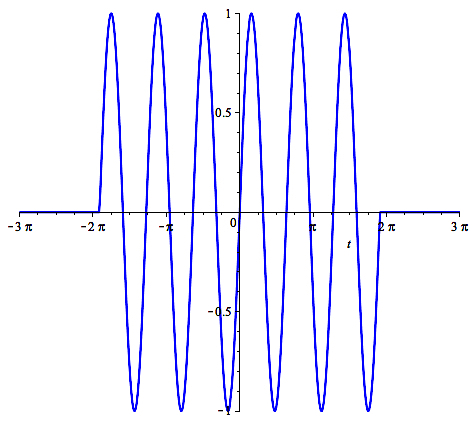
\includegraphics[width=2.6in]{VOLUMEN_1/03_Funciones_Lineales/Figuras/Figura3_5}
\caption{ $f(t)$ con: $n=6$ y $\omega_0=\pi$.}
\label{funciontren}
\end{minipage}
\end{figure}
%%%%%%%%%%%%%%%%%

Resolviendo la integral obtenemos la distribuci�n espectral:
\[
\left|\mathrm{F}(\omega)\right>=
\frac {2 \left[
\omega_0\,\mbox{sen}\left( { \tau \,\omega} \right) \cos \left(n \pi \right)  - \omega\,\cos \left( { \tau \,\omega} \right) \mbox{sen}\left(n \pi \right)  \right] }{\sqrt{2\pi}\left({\omega}^{2}-{\omega_0}^{2}\right)} =
\frac {1}{\sqrt {2\pi }} \left[ \frac {\sin\left[ \tau \left( \omega_0-\omega \right)\right]}{2(\omega_0-\omega)} -\frac {\sin\left[ \tau \left( \omega_0+\omega \right)\right]}{2(\omega_0+\omega)}
 \right] \,,
\]
donde $\tau={\frac {n\pi}{\omega_0}}$.
%%%%%%%%%%%%%%%%%
\begin{figure}[h]
\begin{minipage}{9.0cm}

Se puede demostrar que los l�mites:
\[
\lim_{\omega_0 \rightarrow \infty}\left|\mathrm{F}(\omega)\right>=\lim_{\omega \rightarrow \infty}\left|\mathrm{F}(\omega)\right>=0 \,.
\] 

Se puede apreciar tambi�n que el primer t�rmino, de la expresi�n entre corchetes, es el de mayor relevancia debido a que en el denominador aparece la diferencia: $\omega_0-\omega$. 

En la Figura \ref{Figura3_6} se muestra  la funci�n de distribuci�n y en ella podemos notar que  a medida que $n$ crece la funci�n $\left|\mathrm{F}(\omega)\right>$ es una delta de Dirac en $\omega=\omega_0=\pi$.

Por otro lado, es f�cil ver que los ceros ocurren cuando:
\[
\frac{\omega_0-\omega}{\omega_0}=\pm \frac1n, \pm \frac2n, \pm \frac3n \dots
\]
\end{minipage} \hfill 
\begin{minipage}{6.0cm} 
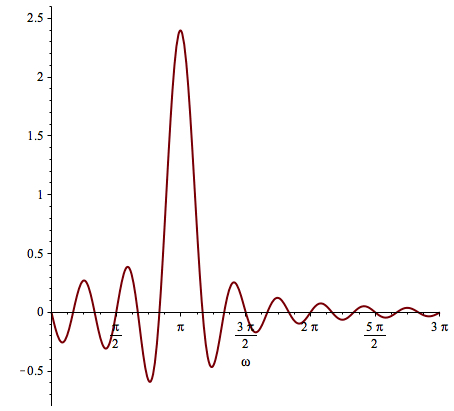
\includegraphics[width=2.4in]{VOLUMEN_1/03_Funciones_Lineales/Figuras/Figura3_6}
\caption{ $\mathrm{F}(\omega)$ con: $n=6$ y $\omega_0=\pi$.}
\label{Figura3_6}
\end{minipage}
\end{figure}
%%%%%%%%%%%%%%%%%

\end{enumerate}

\newpage
\subsection{{\color{red}Practicando con Maxima}}

Estudiaremos en este m�dulo como calcular transformadas integrales de Fourier con {\bf Maxima}. Disponemos de las siguientes funciones: {\bf fourint}(f,x) que calcula y devuelve la lista de los coeficientes integrales de Fourier de $f(x)$ definida en el intervalo $(-\infty, \infty)$. La funci�n {\bf fourintcos} (f,x) que devuelve los coeficientes integrales de los cosenos $f(x)$ en $(0, \infty)$ y la funci�n {\bf fourintsin}(f,x) que retorna los coeficientes integrales de los senos $f(x)$ en $(0, \infty)$

Vamos a aclarar a que se refieren cuando se habla de los coeficientes integrales.
 
Para {\bf Maxima} si $f(x)$ es una funci�n definida en $(-\infty, \infty)$ la transformada de Fourier exponencial es:
\[
F(f,z)=\frac{1}{2\pi}\int_{-\infty}^{\infty} f(x)\ e^{izx} \mathrm{d}x
\,\, \Leftrightarrow \,\, 
f(x)=\int_{-\infty}^{\infty} f(x)\ e^{-izx} \mathrm{d}z\,.
\]

Como vimos anteriormente podemos tener los siguientes casos:
\begin{itemize}
\item La funci�n es par: $f(-x)=f(x)$, entonces: $F(f,-z)=F(f, z)$ y podemos utilizar la representaci�n en transformadas coseno de Fourier:
\[
F(f,z)=\frac12 F_{\mbox{\small cos}}(f,z)\,.
\]

\item La funci�n es impar: $f(-x)=-f(x)$, entonces: $F(f,-z)=-F(f,z)$ y podemos utilizar la representaci�n en transformadas seno de Fourier:
\[
F(f,z)=\frac{i}{2} F_{\mbox{\small sen}}(f,z)\,.
\]

\item La funci�n no es par ni impar. Pero $f(x)$ siempre se puede escribir como la suma de una funci�n par $f_{+}(x)$ y una impar $f_{-}(x)$:
\[
f(x)=f_{+}(x)+f_{-}(x)=\frac{1}{2}\left[f(x)+f(-x) \right]+\frac{1}{2}\left[f(x)-f(-x) \right] \,,
\]
de manera equivalente:
\[
F(f,z)=F(f_{+}+f_{-},z)=\frac{1}{2}F_{\mbox{\small cos}}(f_{+},z)+\frac{i}{2} F_{\mbox{\small sen}}(f_{-}, z) \,.
\]
\end{itemize}

Entonces, la librer�a {\bf fourie} lo que genera es la transformada de Fourier de la forma:
\[
F(f,z)=\frac{1}{2}a_z+\frac{i}{2}b_z \,.
\] 

Veamos algunos ejemplos:


\begin{enumerate}
\item Consideremos la siguiente funci�n par: 
\[
f=x^2 e^{-|x|} \,, \quad \mbox{con  }  x \in (-\infty, \infty) \,.
\]

Podemos intentar resolver la integral que define la transformada de Fourier de manera ``manual'' o directa:
\[
\int_{-\infty}^{\infty} x^2 e^{-|x|} \ e^{-ikx} \mathrm{d}x \,.
\]

%%%%%% INPUT:
\begin{minipage}[t]{8ex}
{\color{red}\bf \begin{verbatim} (%i1) 
\end{verbatim}}
\end{minipage}
\begin{minipage}[t]{\textwidth}{\color{blue}
\begin{verbatim}
f:x^2*exp(-abs(x));
\end{verbatim}}
\end{minipage}

%%% OUTPUT:
\begin{math}\displaystyle \parbox{8ex}{\color{labelcolor}(\%o1) }
x^2\,e^ {- \left| x\right|  }
\end{math}

%%%%%% INPUT:
\begin{minipage}[t]{8ex}
{\color{red}\bf \begin{verbatim} (%i2) 
\end{verbatim}}
\end{minipage}
\begin{minipage}[t]{\textwidth}{\color{blue}
\begin{verbatim}
integrate(exp(-%i*k*x)*f,x,minf,inf);
\end{verbatim}}
\end{minipage}

%%% OUTPUT:
\begin{math}\displaystyle \parbox{8ex}{\color{labelcolor}(\%o2) }
\int_{ -\infty }^{\infty }{x^2\,e^{-\left| x\right| -i\,k\,x}\;dx}
\end{math}
\newline

Lo que significa que el programa no supo resolverla. Intentemos ahora utilizar las funciones propias del programa. 

%%%%%% INPUT:
\begin{minipage}[t]{8ex}
{\color{red}\bf \begin{verbatim} (%i3) 
\end{verbatim}}
\end{minipage}
\begin{minipage}[t]{\textwidth}{\color{blue}
\begin{verbatim}
load(fourie)$
\end{verbatim}}
\end{minipage}


%%%%%% INPUT:
\begin{minipage}[t]{8ex}
{\color{red}\bf \begin{verbatim} (%i4) 
\end{verbatim}}
\end{minipage}
\begin{minipage}[t]{\textwidth}{\color{blue}
\begin{verbatim}
fourint(f,x);
\end{verbatim}}
\end{minipage}

%%% OUTPUT:
\begin{math}\displaystyle \parbox{8ex}{\color{labelcolor}(\%t4) }
a_{z}=\frac{2\,\left(\frac{2}{z^6+3\,z^4+3\,z^2+1}-\frac{6\,z^2}{z^
 6+3\,z^4+3\,z^2+1}\right)}{\pi}
\end{math}

%%% OUTPUT:
\begin{math}\displaystyle \parbox{8ex}{\color{labelcolor}(\%t5) }
b_{z}=0
\end{math}

%%% OUTPUT:
\begin{math}\displaystyle \parbox{8ex}{\color{labelcolor}(\%o5) }
\left[ {\tt \%t4} , {\tt \%t5} \right]
\end{math}

%%%%%% INPUT:
\begin{minipage}[t]{8ex}
{\color{red}\bf \begin{verbatim} (%i6) 
\end{verbatim}}
\end{minipage}
\begin{minipage}[t]{\textwidth}{\color{blue}
\begin{verbatim}
ratsimp(%t4),factor;
\end{verbatim}}
\end{minipage}

%%% OUTPUT:
\begin{math}\displaystyle \parbox{8ex}{\color{labelcolor}(\%o6) }
a_{z}=-\frac{4\,\left(3\,z^2-1\right)}{\pi\,\left(z^2+1\right)^3}
\end{math}
\newline

Esta es la notaci�n que el programa utiliza para decirnos que la transformada es
\[
F(k)=\frac12\left[-\frac{4\,\left(3\,k^2-1\right)}{\pi\,\left(k^2+1\right)^3}\right]=-\frac{2\,\left(3\,k^2-1\right)}{\pi\,\left(k^2+1\right)^3} \,.
\]

Notemos que el c�lculo anterior se corresponde a la transformada coseno de Fourier:

%%%%%% INPUT:
\begin{minipage}[t]{8ex}
{\color{red}\bf \begin{verbatim} (%i17) 
\end{verbatim}}
\end{minipage}
\begin{minipage}[t]{\textwidth}{\color{blue}
\begin{verbatim}
fourintcos(f,x);
\end{verbatim}}
\end{minipage}

%%% OUTPUT:
\begin{math}\displaystyle \parbox{8ex}{\color{labelcolor}(\%t7) }
a_{z}=\frac{2\,\left(\frac{2}{z^6+3\,z^4+3\,z^2+1}-\frac{6\,z^2}{z^
 6+3\,z^4+3\,z^2+1}\right)}{\pi}
\end{math}

%%% OUTPUT:
\begin{math}\displaystyle \parbox{8ex}{\color{labelcolor}(\%o7) }
\left[ {\tt \%t{7}} \right] 
\end{math}

%%%%%% INPUT:
\begin{minipage}[t]{8ex}
{\color{red}\bf \begin{verbatim} (%i8) 
\end{verbatim}}
\end{minipage}
\begin{minipage}[t]{\textwidth}{\color{blue}
\begin{verbatim}
ratsimp(%t7),factor;
\end{verbatim}}
\end{minipage}

%%% OUTPUT:
\begin{math}\displaystyle \parbox{8ex}{\color{labelcolor}(\%o8) }
a_{z}=-\frac{4\,\left(3\,z^2-1\right)}{\pi\,\left(z^2+1\right)^3}
\end{math}
\newline

Podemos intentar resolver directamente la integral para la transformada coseno de Fourier. Para tal fin escribimos toda la expresi�n a resolver.

%%%%%% INPUT:
\begin{minipage}[t]{8ex}
{\color{red}\bf \begin{verbatim} (%i9) 
\end{verbatim}}
\end{minipage}
\begin{minipage}[t]{\textwidth}{\color{blue}
\begin{verbatim}
Fz:ratsimp(1/%pi*integrate(cos(x*z)*f,x,0,inf)),factor;
\end{verbatim}}
\end{minipage}

%%% OUTPUT:
\begin{math}\displaystyle \parbox{8ex}{\color{labelcolor}(\%o9) }
-\frac{2\,\left(3\,z^2-1\right)}{\pi\,\left(z^2+1\right)^3}
\end{math}
\newline

Incluso podemos probar calculando la transformada inversa y verificar que los c�lculos son correctos.

%%%%%% INPUT:
\begin{minipage}[t]{8ex}
{\color{red}\bf \begin{verbatim} (%i10) 
\end{verbatim}}
\end{minipage}
\begin{minipage}[t]{\textwidth}{\color{blue}
\begin{verbatim}
integrate(exp(-%i*z*x)*Fz,z,minf,inf);
\end{verbatim}}
\end{minipage}
{\color{red}Is x positive, negative or zero?} p;

%%% OUTPUT:
\begin{math}\displaystyle \parbox{8ex}{\color{labelcolor}(\%o10) }
x^2\,e^ {- x }
\end{math}

%%%%%% INPUT:
\begin{minipage}[t]{8ex}
{\color{red}\bf \begin{verbatim} (%i11) 
\end{verbatim}}
\end{minipage}
\begin{minipage}[t]{\textwidth}{\color{blue}
\begin{verbatim}
integrate(exp(-%i*z*x)*Fz,z,minf,inf);
\end{verbatim}}
\end{minipage}
{\color{red}Is x positive, negative or zero?} n;

%%% OUTPUT:
\begin{math}\displaystyle \parbox{8ex}{\color{labelcolor}(\%o11) }
x^2\,e^ {x }
\end{math}


\item Consideremos la siguiente funci�n impar:
\[
f=x e^{-|x|} \,.
\]

%%%%%% INPUT:
\begin{minipage}[t]{8ex}
{\color{red}\bf \begin{verbatim} (%i12) 
\end{verbatim}}
\end{minipage}
\begin{minipage}[t]{\textwidth}{\color{blue}
\begin{verbatim}
f:x*exp(-abs(x));
\end{verbatim}}
\end{minipage}

%%% OUTPUT:
\begin{math}\displaystyle \parbox{8ex}{\color{labelcolor}(\%o12) }
x\,e^ {- \left| x\right|  }
\end{math}

%%%%%% INPUT:
\begin{minipage}[t]{8ex}
{\color{red}\bf \begin{verbatim} (%i13) 
\end{verbatim}}
\end{minipage}
\begin{minipage}[t]{\textwidth}{\color{blue}
\begin{verbatim}
fourint(f,x);
\end{verbatim}}
\end{minipage}

%%% OUTPUT:
\begin{math}\displaystyle \parbox{8ex}{\color{labelcolor}(\%t13) }
a_{z}=0
\end{math}

%%% OUTPUT:
\begin{math}\displaystyle \parbox{8ex}{\color{labelcolor}(\%t14) }
b_{z}=\frac{4\,z}{\pi\,\left(z^4+2\,z^2+1\right)}
\end{math}

%%% OUTPUT:
\begin{math}\displaystyle \parbox{8ex}{\color{labelcolor}(\%o14) }
\left[ {\tt \%t13} , {\tt \%t14} \right]
\end{math}


%%%%%% INPUT:
\begin{minipage}[t]{8ex}
{\color{red}\bf \begin{verbatim} (%i15) 
\end{verbatim}}
\end{minipage}
\begin{minipage}[t]{\textwidth}{\color{blue}
\begin{verbatim}
ratsimp(%t14),factor;
\end{verbatim}}
\end{minipage}

%%% OUTPUT:
\begin{math}\displaystyle \parbox{8ex}{\color{labelcolor}(\%o15) }
b_{z}=\frac{4\,z}{\pi\,\left(z^2+1\right)^2}
\end{math}


%%%%%% INPUT:
\begin{minipage}[t]{8ex}
{\color{red}\bf \begin{verbatim} (%i16) 
\end{verbatim}}
\end{minipage}
\begin{minipage}[t]{\textwidth}{\color{blue}
\begin{verbatim}
fourintsin(f,x);
\end{verbatim}}
\end{minipage}

%%% OUTPUT:
\begin{math}\displaystyle \parbox{8ex}{\color{labelcolor}(\%t16) }
b_{z}=\frac{4\,z}{\pi\,\left(z^4+2\,z^2+1\right)}
\end{math}

%%% OUTPUT:
\begin{math}\displaystyle \parbox{8ex}{\color{labelcolor}(\%o16) }
\left[ {\tt \%t16} \right]
\end{math}

%%%%%% INPUT:
\begin{minipage}[t]{8ex}
{\color{red}\bf \begin{verbatim} (%i17) 
\end{verbatim}}
\end{minipage}
\begin{minipage}[t]{\textwidth}{\color{blue}
\begin{verbatim}
ratsimp(%t16),factor;
\end{verbatim}}
\end{minipage}

%%% OUTPUT:
\begin{math}\displaystyle \parbox{8ex}{\color{labelcolor}(\%o17) }
b_{z}=\frac{4\,z}{\pi\,\left(z^2+1\right)^2}
\end{math}
\newline

Esto significa que la transformada seno de Fourier es:
\[
F(k)=\frac{i}{2}\left[\frac{4\,k}{\pi\,\left(k^2+1\right)^2}\right]=
\frac{2 i \,k}{\pi\,\left(k^2+1\right)^2} \,.
\]

Realicemos nuevamente el c�lculo pero integrando  para comparar.

%%%%%% INPUT:
\begin{minipage}[t]{8ex}
{\color{red}\bf \begin{verbatim} (%i18) 
\end{verbatim}}
\end{minipage}
\begin{minipage}[t]{\textwidth}{\color{blue}
\begin{verbatim}
Fz:%i*ratsimp(1/%pi*integrate(sin(x*z)*f,x,0,inf)),factor;
\end{verbatim}}
\end{minipage}

%%% OUTPUT:
\begin{math}\displaystyle \parbox{8ex}{\color{labelcolor}(\%o18) }
\frac{2\,i\,z}{\pi\,\left(z^2+1\right)^2}
\end{math}
\newline

Vamos a calcular la transformada inversa:

%%%%%% INPUT:
\begin{minipage}[t]{8ex}
{\color{red}\bf \begin{verbatim} (%i19) 
\end{verbatim}}
\end{minipage}
\begin{minipage}[t]{\textwidth}{\color{blue}
\begin{verbatim}
integrate(exp(-%i*z*x)*Fz,z,minf,inf);
\end{verbatim}}
\end{minipage}
{\color{red}Is x positive, negative or zero?} p;

%%% OUTPUT:
\begin{math}\displaystyle \parbox{8ex}{\color{labelcolor}(\%o19) }
x\,e^ {- x }
\end{math}

%%%%%% INPUT:
\begin{minipage}[t]{8ex}
{\color{red}\bf \begin{verbatim} (%i20) 
\end{verbatim}}
\end{minipage}
\begin{minipage}[t]{\textwidth}{\color{blue}
\begin{verbatim}
integrate(exp(-%i*z*x)*Fz,z,minf,inf);
\end{verbatim}}
\end{minipage}
{\color{red}Is x positive, negative or zero?} n;

%%% OUTPUT:
\begin{math}\displaystyle \parbox{8ex}{\color{labelcolor}(\%o20) }
x\,e^ {x }
\end{math}
\newline

\item Dada la siguiente funci�n que no es par ni impar:
\[
f(x)=(x-1)e^{(-|x|)}\,.
\]

%%%%%% INPUT:
\begin{minipage}[t]{8ex}
{\color{red}\bf \begin{verbatim} (%i21) 
\end{verbatim}}
\end{minipage}
\begin{minipage}[t]{\textwidth}{\color{blue}
\begin{verbatim}
f:(x-1)*exp(-abs(x));
\end{verbatim}}
\end{minipage}

%%% OUTPUT:
\begin{math}\displaystyle \parbox{8ex}{\color{labelcolor}(\%o21) }
\left(x-1\right)\,e^ {- \left| x\right|  }
\end{math}

%%%%%% INPUT:
\begin{minipage}[t]{8ex}
{\color{red}\bf \begin{verbatim} (%i22) 
\end{verbatim}}
\end{minipage}
\begin{minipage}[t]{\textwidth}{\color{blue}
\begin{verbatim}
fourint(f,x);
\end{verbatim}}
\end{minipage}

%%% OUTPUT:
\begin{math}\displaystyle \parbox{8ex}{\color{labelcolor}(\%t22) }
a_{z}=-\frac{2}{\pi\,\left(z^2+1\right)}
\end{math}

%%% OUTPUT:
\begin{math}\displaystyle \parbox{8ex}{\color{labelcolor}(\%t23) }
b_{z}=\frac{4\,z}{\pi\,\left(z^4+2\,z^2+1\right)}
\end{math}

%%% OUTPUT:
\begin{math}\displaystyle \parbox{8ex}{\color{labelcolor}(\%o23) }
\left[ {\tt \%t{22}} , {\tt \%t{23}} \right]
\end{math}

%%%%%% INPUT:
\begin{minipage}[t]{8ex}
{\color{red}\bf \begin{verbatim} (%i24) 
\end{verbatim}}
\end{minipage}
\begin{minipage}[t]{\textwidth}{\color{blue}
\begin{verbatim}
az:ratsimp(%t22),factor; bz:ratsimp(%t23),factor;
\end{verbatim}}
\end{minipage}

%%% OUTPUT:
\begin{math}\displaystyle \parbox{8ex}{\color{labelcolor}(\%o24) }
a_{z}=-\frac{2}{\pi\,\left(z^2+1\right)}
\end{math}

%%% OUTPUT:
\begin{math}\displaystyle \parbox{8ex}{\color{labelcolor}(\%o25) }
b_{z}=\frac{4\,z}{\pi\,\left(z^2+1\right)^2}
\end{math}

%%%%%% INPUT:
\begin{minipage}[t]{8ex}
{\color{red}\bf \begin{verbatim} (%i26) 
\end{verbatim}}
\end{minipage}
\begin{minipage}[t]{\textwidth}{\color{blue}
\begin{verbatim}
Fz:1/2*rhs(az)+%i/2*rhs(bz),factor;
\end{verbatim}}
\end{minipage}

%%% OUTPUT:
\begin{math}\displaystyle \parbox{8ex}{\color{labelcolor}(\%o26) }
-\frac{z^2-2\,i\,z+1}{\pi\,\left(z^2+1\right)^2}
\end{math}
\newline

De nuevo,  la transformada inversa para verificar:

%%%%%% INPUT:
\begin{minipage}[t]{8ex}
{\color{red}\bf \begin{verbatim} (%i27) 
\end{verbatim}}
\end{minipage}
\begin{minipage}[t]{\textwidth}{\color{blue}
\begin{verbatim}
integrate(exp(-%i*z*x)*Fz,z,minf,inf);
\end{verbatim}}
\end{minipage}
{\color{red}Is x positive, negative or zero?} p;

%%% OUTPUT:
\begin{math}\displaystyle \parbox{8ex}{\color{labelcolor}(\%o27) }
(x-1)\,e^ {- x }
\end{math}

%%%%%% INPUT:
\begin{minipage}[t]{8ex}
{\color{red}\bf \begin{verbatim} (%i28) 
\end{verbatim}}
\end{minipage}
\begin{minipage}[t]{\textwidth}{\color{blue}
\begin{verbatim}
integrate(exp(-%i*z*x)*Fz,z,minf,inf);
\end{verbatim}}
\end{minipage}
{\color{red}Is x positive, negative or zero?} n;

%%% OUTPUT:
\begin{math}\displaystyle \parbox{8ex}{\color{labelcolor}(\%o28) }
(x-1)\,e^ {x }
\end{math}

%%%%%% INPUT:
\begin{minipage}[t]{8ex}
{\color{red}\bf \begin{verbatim} (%i29) 
\end{verbatim}}
\end{minipage}
\begin{minipage}[t]{\textwidth}{\color{blue}
\begin{verbatim}
kill(all)$
\end{verbatim}}
\end{minipage}

\item Resolvamos ahora el ejemplo \ref{ejemplo5s35} donde la funci�n era:
\[
f(t)=\mbox{sen}(\omega_0 t) \,.
\]

%%%%%% INPUT:
\begin{minipage}[t]{8ex}
{\color{red}\bf \begin{verbatim} (%i1) 
\end{verbatim}}
\end{minipage}
\begin{minipage}[t]{\textwidth}{\color{blue}
\begin{verbatim}
load(fourie)$
\end{verbatim}}
\end{minipage}

%%%%%% INPUT:
\begin{minipage}[t]{8ex}
{\color{red}\bf \begin{verbatim} (%i2) 
\end{verbatim}}
\end{minipage}
\begin{minipage}[t]{\textwidth}{\color{blue}
\begin{verbatim}
f:sin(w0*t);
\end{verbatim}}
\end{minipage}

%%% OUTPUT:
\begin{math}\displaystyle \parbox{8ex}{\color{labelcolor}(\%o2) }
\sin \left({\tt w0}\,t\right)
\end{math}
\newline

Como la funci�n es impar, podemos intentar: 

%%%%%% INPUT:
\begin{minipage}[t]{8ex}
{\color{red}\bf \begin{verbatim} (%i3) 
\end{verbatim}}
\end{minipage}
\begin{minipage}[t]{\textwidth}{\color{blue}
\begin{verbatim}
fourintsin(f,t);
\end{verbatim}}
\end{minipage}

%%% OUTPUT:
\begin{math}\displaystyle \parbox{8ex}{\color{labelcolor}(\%t3) }
b_{z}=\frac{2\,\left(\lim_{t\rightarrow \infty }{-\frac{\sin \left(t\,
 z+{\tt w0}\,t\right)}{2\,z+2\,{\tt w0}}-\frac{\sin \left(t
 \,z-{\tt w0}\,t\right)}{2\,{\tt w0}-2\,z}}\right)}{\pi}
\end{math}

\begin{math}\displaystyle \parbox{8ex}{\color{labelcolor}(\%o3) }
\left[ {\tt \%t3} \right] 
\end{math}
\newline

�Intento fallido! Podemos probar resolviendo la integral.

%%%%%% INPUT:
\begin{minipage}[t]{8ex}
{\color{red}\bf \begin{verbatim} (%i4) 
\end{verbatim}}
\end{minipage}
\begin{minipage}[t]{\textwidth}{\color{blue}
\begin{verbatim}
tau:n*%pi/w0;
\end{verbatim}}
\end{minipage}

%%%%%% INPUT:
\begin{minipage}[t]{8ex}
{\color{red}\bf \begin{verbatim} (%i5) 
\end{verbatim}}
\end{minipage}
\begin{minipage}[t]{\textwidth}{\color{blue}
\begin{verbatim}
Fw:sqrt(2/%pi)*ratsimp(integrate(sin(t*omega)*f,t,0,tau));
\end{verbatim}}
\end{minipage}
{\color{red}Is nw0 positive, negative or zero?} p;

%%% OUTPUT:
\begin{math}\displaystyle \parbox{8ex}{\color{labelcolor}(\%o5) }
-\frac{\sqrt{2}\,\left(\left({\tt w0}-\omega\right)\,\sin 
 \left(\frac{\pi\,n\,{\tt w0}+\pi\,n\,\omega}{{\it w0}}
 \right)+\left(-{\tt w0}-\omega\right)\,\sin \left(\frac{\pi\,n
 \,{\tt w0}-\pi\,n\,\omega}{{\tt w0}}\right)\right)}{\sqrt{
 \pi}\,\left(2\,{\tt w0}^2-2\,\omega^2\right)}
\end{math}

Asignemos los valores num�ricos a los par�metros:

%%%%%% INPUT:
\begin{minipage}[t]{8ex}
{\color{red}\bf \begin{verbatim} (%i6) 
\end{verbatim}}
\end{minipage}
\begin{minipage}[t]{\textwidth}{\color{blue}
\begin{verbatim}
n:6$ w0:%pi$
\end{verbatim}}
\end{minipage}


%%%%%% INPUT:
\begin{minipage}[t]{8ex}
{\color{red}\bf \begin{verbatim} (%i7) 
\end{verbatim}}
\end{minipage}
\begin{minipage}[t]{\textwidth}{\color{blue}
\begin{verbatim}
Fw:ev(Fw);
\end{verbatim}}
\end{minipage}

%%% OUTPUT:
\begin{math}\displaystyle \parbox{8ex}{\color{labelcolor}(\%o7) }
-\frac{\sqrt{2}\,\left(\left(\pi-\omega\right)\,\sin \left(\frac{6
 \,\pi\,\omega+6\,\pi^2}{\pi}\right)+\left(-\omega-\pi\right)\,\sin 
 \left(\frac{6\,\pi^2-6\,\pi\,\omega}{\pi}\right)\right)}{\sqrt{\pi}
 \,\left(2\,\pi^2-2\,\omega^2\right)}
\end{math}
\newline

Grafiquemos ahora la transformada $F(w)$:

%%%%%% INPUT:
\begin{minipage}[t]{8ex}
{\color{red}\bf \begin{verbatim} (%i8) 
\end{verbatim}}
\end{minipage}
\begin{minipage}[t]{\textwidth}{\color{blue}
\begin{verbatim}
wxplot2d([Fw], [omega,0,3*%pi])$
\end{verbatim}}
\end{minipage}


%%% OUTPUT:
\begin{math}\displaystyle \parbox{8ex}{\color{labelcolor}(\%o8) }
\end{math}

\begin{figure}[h]\nonumber
\begin{center}
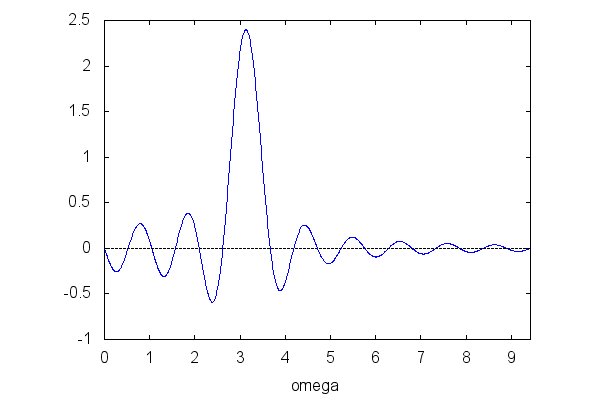
\includegraphics[height=2.6in,width=4.5in]{VOLUMEN_1/03_Funciones_Lineales/Figuras/Figura3_7.jpg}
\end{center}
\end{figure}


\end{enumerate}


\begin{center}
{\color{red}\rule{15.8cm}{0.4mm}}
\end{center}



\subsection{{\color{OliveGreen}Ejercicios}}
\begin{enumerate}
\item Si: 
\[
\delta_n(x)=\left\{
\begin{array}{cl}
0 & x< -\frac{1}{2n} \\
n & -\frac{1}{2n}< x < \frac{1}{2n}\\
0 & x<\frac{1}{2n}
\end{array}
\right.
\]
demuestre que:
\[
f(0)= \lim_{n \rightarrow \infty}\int_{-\infty}^{\infty} f(x)\delta_{n}(x) \mathrm{d}x \,,
\]
para $f(x)$ continua en $x=0$.

\item Para: 
\[
\delta_n(x)=\frac{n}{\pi}\frac{1}{1+n^2x^2}\,.
\]
Demuestre lo siguiente:
\[
\int_{-\infty}^{\infty} \delta_{n}(x) \mathrm{d}x=1 \,.
\]

\item Si:
\[
\delta_n(x)=\frac{n}{\sqrt{\pi}}\mathrm{e}^{-n^2x^2}\,.
\]
Demuestre que:
\[
x\frac{\mathrm{d}\delta(x)}{\mathrm{d} x}= -\delta(x) \,.
\]


\item Demuestre la siguiente relaci�n:
\[
\int_{-\infty}^{\infty} \delta'(x)f(x) \mathrm{d}x= -f(0) \,.
\]  

\item Dadas las siguientes funciones ortonormales:
\begin{eqnarray*}
\mbox{a)}\,\,\, \left|  \mathrm{e}(k,x)\right> &=& 
\left\{\frac{1}{\sqrt{\pi}}\mbox{sen}(kx)\,,\frac{1}{\sqrt{\pi}}\cos(kx)\right\} \,, \,\,\, \mbox{con: }\,\,\, 
0\leq k < \infty \,,  -\infty\leq x < \infty \,. \\
\mbox{b)}\,\,\, \left|  \mathrm{e}(k,x)\right> &=&
\left\{\frac{1}{\sqrt{2\pi}} \mathrm{e}^{ikx} \right\} \,, \,\,\, \mbox{con: }\,\,\, -\infty \leq k < \infty \,,  -\infty \leq x < \infty \,.
\end{eqnarray*}

\begin{enumerate}
\item Escriba las condiciones de ortogonalidad y cierre.
\item Demuestre:
\begin{enumerate}
\item $\int_{-\infty}^{\infty} \mbox{sen}(kx)\mbox{sen}(k'x) \mathrm{d}x=
\pi\delta(k-k')$.
\item $\int_{-\infty}^{\infty} \cos(kx)\cos(k'x) \mathrm{d}x=\pi\delta(k-k')$.
\item $\int_{-\infty}^{\infty} \mbox{sen}(kx)\cos(k'x) \mathrm{d}x=0$.
\end{enumerate}

\end{enumerate}

\item Demuestre que si:
\[
\delta_n(x)=\frac{n}{\pi(1+n^2x^2)} \,,
\]
entonces:
\[
\int_{-\infty}^{\infty} \delta_n \mathrm{d}x=1\,. 
\]

\item Dada la siguiente sucesi�n de funciones:
\[
\delta_n(x)=\frac{1}{2n \pi }\left(\frac{\mbox{sen}(nx/2)}{\mbox{sen}(x/2)}\right)^2 \,.
\]
Demuestre que $\delta_n(x)$ es una distribuci�n delta de Dirac  al calcular
\[
\lim_{n \rightarrow \infty} \left[\frac{1}{2n \pi}\int_{-\infty}^{\infty}
f(x)\left(\frac{\mbox{sen}(nx/2)}{\mbox{sen}(x/2)}\right)^2 \mathrm{d}x\right] =f(0)\,.
\]

\item Encuentre las transformadas de Fourier de las siguientes funciones:

\[
a) \quad 
f(x)=\left\{
\begin{array}{cc}
\mathrm{e}^{-x}\,,& x > 0 \\
 & \\
0\,, & x<0
\end{array}
\right. \qquad \qquad 
b) \quad 
f(x)=\left\{
\begin{array}{cc}
h(1-a |x|)\,,& |x| < \frac1a \\
 & \\
0\,, & |x| > \frac1a
\end{array}
\right. 
\]

\item Dad  $F({\bf k})$ como la transformada de Fourier, en tres dimensiones, de $f({\bf r})$ y
$F_d({\bf k})$ la transformada de Fourier, tridimensional, de ${\boldsymbol \nabla} f({\bf r}) $. Demuestre que:
\[
F_d({\bf k})= -i{\bf k}({\bf k}) \,.
\] 

\item Resuelva los ejercicios anteriores con {\bf Maxima}. 


\end{enumerate}

\begin{thebibliography}{9}
\bibitem{ArfkenWeberWeber2000}  Arfken, G. B.,Weber, H., Weber, H.J. (2000) \textbf{Mathematical Methods for Physicists} 5ta Edici�n (Academic Press, Nueva York)

\bibitem{BorisenkoTarapov1968}  Borisenko, A.I, y Tarapov I.E. (1968) \textbf{Vector and Tensor Analisys} (Dover Publications Inc, Nueva York)

\bibitem{DennerykKrzywicki1995}  Dennery, P. y Krzywicki, A. (1995) \textbf{Mathematics for Physicists} (Dover Publications Inc, Nueva York)

\bibitem{Harper1971}  Harper, C. (1971) \textbf{Introduction to Mathematical Physics} (\textit{Prentice Hall, Englewood Cliff, N.J:})

\bibitem{Hassani1991}  Hassani, S. (1991) \textbf{Foundations of Mathematical Physics} (\textit{Prentice Hall, International Edition, London:}

\bibitem{Hauser1971}  Hauser, W (1971) \textbf{Introduction to Principles of Electromagnetism }\ (\textit{Addison-Wesley Pub Co Reading})

\bibitem{RileyHobsonBence2002}  Riley, K.F., Hobson, M.P. y Bence, S.J. (2002) \textbf{Mathematical Methods for Physics and Engineering } (\textit{Cambridge University Press})

\bibitem{Santalo1969}  Santal�, L.A (1969) \textbf{Vectores y Tensores} (\textit{Editorial Universitaria, Buenos Aires})

\bibitem{Schutz1980}  Schutz, B. (1980) \textbf{Geometrical Methods in Mathematical Physics} (\textit{Cambridge University Press, Londres})

 \bibitem{Spiegel1959}  Spiegel, M. (1959) \textbf{Vector Analysis }(\textit{Schaums Outline Series, McGraw Hill New York})
\end{thebibliography}


\chapter{Matrices, determinantes y autovectores}
\label{CapMatricesDeterminantesAutovectores}

\section*{La ruta de este cap�tulo}

En el cap�tulo anterior definimos los funcionales lineales como un {\it morfismo} de un espacio vectorial lineal $\textbf{\em V}$ a un espacio unidimensional $\textbf{\em K}$. Esta misma idea se puede extender a morfismos de un espacio vectorial $\textbf{\em V}_{1}$ a un espacio vectorial $\textbf{\em V}_{2}$, sobre el mismo campo $\textbf{\em K}$. Desarrollaremos estos conceptos a trav�s de los operadores lineales en la secci�n \ref{OperadoresLineales}, y en la secci�n \ref{Tiposdeoperadores} se�alaremos algunos de los operadores lineales de mayor relevancia. En la secci�n \ref{RepresentacionMatricialOpe} estableceremos una correspondencia uno-a-uno entre operadores lineales y matrices y la dependencia de �sta correspondencia con las bases del espacio vectorial. Luego, en la secci�n \ref{zoologicodematrices}  presentaremos un conjunto de matrices fundamentales junto con sus  operaciones. En la secci�n \ref{SistemasEcuacionesLineales}, veremos algunos de los m�todos m�s comunes para la resoluci�n de sistemas de ecuaciones lineales. Y para finalizar, las secciones  \ref{SecAutovectoresAutovalores} y \ref{autovectoresmatricesimportantes} estar�n dedicadas al importante tema de la representaci�n espectral de un operador: el problema de autovalores y autovectores. 

\section{Operadores lineales}
\label{OperadoresLineales}
\index{Operador Lineal}
\index{Lineal!Operador}

Definiremos como operador lineal (o transformaci�n lineal) a una operaci�n que asocia un vector $\left| {v}\right> \in \textbf{\em V}_{1}$ un vector $\left|  {v}^{\prime}\right> \in \textbf{\em V}_{2}$ y que respeta la linealidad, es decir esta funci�n de $\textbf{\em V}_{1} \rightarrow \textbf{\em V}_{2}$ cumple con:
\begin{equation}
\label{OperadorLineal}
\left|  {v}^{\prime}\right> =\mathbb{T}\left|  {v} \right> \quad /  \quad 
\mathbb{T}\left[  \alpha\ \left|  {v}_{{1}}\right> +\beta\ \left|  {v}_{2}\right> \right]  =
\alpha\ \mathbb{T}\left|  {v}_{{1}}\right> +\beta\ \mathbb{T}\left|  {v}_{2}\right> \,\, \forall \,\,
\quad \left|  {v}_{{1} }\right> \text{ y }\left|  {v}_{2}\right> \in\textbf{\em V}_{1} \,.
\end{equation}

Sencillamente, algo que act�e sobre una suma de vectores en  
$\textbf{\em V}_{1}$  y que es equivalente a la suma de sus actuaciones sobre los vectores suma, es decir, a la suma en $\textbf{\em V}_{2}$. 

Podemos ilustrar este tipo de transformaci�n con varios ejemplos:
\begin{enumerate}
\item  Las siguientes transformaciones: 
$\left|x^{\prime}\right>=\mathbb{T}\left| x \right> \,\, \rightarrow \,\,
\left(x^{\prime},y^{\prime},z^{\prime}\right)  =
\mathbb{T}\left\{\left(x,y,z\right)  \right\}$,  claramente son lineales

\begin{itemize}
\item $\mathbb{T}\left[ \left(x,y,z\right) \right]=\left(x,2y,3z\right) $
\[ 
\mathbb{T}\left[\alpha \left(x_1,y_1,z_1\right) +\beta \left(x_2,y_2,z_2\right)  \right]= 
\alpha \mathbb{T}\left[ \left(x_1,y_1,z_1\right)  \right]  +
\beta   \mathbb{T}\left[\left(x_2,y_2,z_2\right)  \right] \,,
\]
entonces:
\begin{eqnarray*}
\mathbb{T}\left[\left( \alpha x_1+\beta x_2,\alpha y_1+\beta y_2,\alpha z_1+\beta z_2\right)  \right] &=&
\alpha\left(x_1, 2y_1,3z_1\right)  +\beta \left(x_2,2y_2,3z_2\right) \\
\left( \alpha x_1+\beta x_2, 2\left[  \alpha y_1+\beta y_2\right]  ,3\left[ \alpha z_1+\beta z_2 \right]  \right)  & =&
\left( \alpha x_1+\beta x_2, 2\left[ \alpha y_1+\beta y_2 \right]  ,3\left[ \alpha z_1+\beta z_2 \right]  \right) \,.
\end{eqnarray*}

\item $\mathbb{T}\left\{  \left(x,y,z\right)  \right\} =\left( z,y,x\right)$
\[ 
\mathbb{T}\left[\alpha \left(x_1,y_1,z_1\right) +\beta \left(x_2,y_2,z_2\right)  \right]= 
\alpha \mathbb{T}\left[ \left(x_1,y_1,z_1\right)  \right]  +
\beta   \mathbb{T}\left[\left(x_2,y_2,z_2\right)  \right] \,,
\]
igual que en el caso anterior:
\begin{eqnarray*}
\mathbb{T}\left\{  \left(\alpha x_1+\beta x_2, \alpha y_1+\beta y_2, \alpha z_1+\beta z_2 \right)  \right\} &=&
\alpha \left( z_1, y_1, x_1\right)  +\beta \left( z_2, y_2, x_2\right) \\
\left(  \alpha z_1+\beta z_2, \alpha y_1+\beta y_2, \alpha x_1+\beta x_2\right)   & =&
\left(  \alpha z_1+\beta z_2, \alpha y_1+\beta y_2, \alpha x_1+\beta x_2\right) \,.
\end{eqnarray*}

\end{itemize}

\item  Cosas tan sencillas como la multiplicaci�n por un n�mero es una transformaci�n (u operador) lineal, esto es, una transformaci�n $\mathbb{T}:\textbf{\em V} \rightarrow \textbf{\em V}$ tal que
\[
\mathbb{T}\left|  {v}\right> =\left|  {v}^{\prime }\right> =\lambda \left|  {v}\right> \,\, \Rightarrow  \,\, 
\mathbb{T}\left[  \alpha\left|  {v}\right> +\beta \left|  {w}\right> \right]  =  \alpha\mathbb{T}\left|  {v}\right> +\beta\mathbb{T}\left|  {w}\right> = \alpha\lambda\left| v\right> +\beta\lambda\left| {w}\right> \,.
\]
Obviamente, si $\lambda=1$ tenemos la transformaci�n identidad que transforma todo vector en s� mismo; si $\lambda=0$ tendremos la transformaci�n cero, vale decir que lleva a todo $\left| {v} \right> \in\textbf{\em V}$ a al elemento cero $\left|  {0}\right> $.

\item  La definici�n de producto interno tambi�n puede ser vista como una transformaci�n (operador) lineal 
$\mathbb{T} :\textbf{\em V}\rightarrow \mathds{R} $
\[
\mathbb{T}\left|  {v}\right> =\lambda \rightleftharpoons \left< {u}\right.  \left|  {v}\right> \equiv \lambda \, .
\]
Otra vez:
\[
\mathbb{T}\left[  \alpha\left|  {v}\right> +\beta\left|  {w}\right> \right]  =\left< {u}\right|  \left[  \alpha\left| {v}\right> +\beta\left|  {w}\right> \right]
=\alpha\left< {u}\right.  \left|  {v}\right> +\beta\left< {u}\right.  \left|  {w}\right> \, ,
\]
por lo tanto es lineal. Esto implica que tambi�n la proyecci�n de un determinado $\left| {v}\right> \in\textbf{\em V}$ sobre un subespacio $\textbf{\em S}$ es un operador lineal, y lo denotaremos como:
\[
\left[  \left|  {s}\right> \left< {s}\right| \right]  \ \left|  {v}\right> =\left< {s}\right.
\left|  {v}\right> \left|  {s}\right> =\left| {v}_{s}\right> \,,\quad\text{con }\left|  {s}\right>  \text{\ y }\left|  {v}_{s}\right> \in\textbf{\em S}\,.
\]
Esta idea se extiende f�cilmente para un proyector $\mathbb{T}:\textbf{\em V}_{m}\mathbf{\rightarrow S}_{n}$ con $m>n$, de tal modo que para un vector $\left| {v}\right> \in\textbf{\em V}_{m}$
\[
\mathbb{P}_{m}\left|  {v}\right> \equiv\left(  \left|{u}_{i}\right> \left< {u}^{i}\right|  _{m}\right)
\left|  {v}\right> =\left< {u}^{i}\right.  \left| {v}\right> _{m}\left|  {u}_{i}\right> =\left| {v}_{m}\right> \, ,
\]
con $\left\{  \left< {u}_{i}\right|  \right\} $ una base de $\textbf{\em S}_{n}$. Es claro que estamos utilizando la convenci�n de Einstein para la suma de �ndices.

\item  Las ecuaciones lineales tambi�n pueden verse como transformaciones lineales. Esto es, considere una transformaci�n lineal $\mathbb{T} :\textbf{\em V}_{n} \mathbf{\rightarrow V}_{m}$. Por lo tanto asociaremos
\[
\left|  {y}\right> =\mathbb{T}\left| {x}\right> \,\, \Rightarrow \,\,  \left(  y^{1},y^{2},y^{3},\cdots,y^{m}\right)
=\mathbb{T}\left[ \left(  x^{1},x^{2},x^{3},\cdots,x^{n}\right)  \right] \, ,
\]
a trav�s de $n\times m$ n�meros, $a_{j}^{i}$, organizados de la siguiente forma:
\[
y^{i}=a_{j}^{i}\ x^{j} \qquad \text{con }
\left\{
\begin{array}
[c]{c}
i=1,2,\cdots,m\\
j=1,2,\cdots,n
\end{array}
\right.
\]
una vez m�s,
\begin{align*}
\mathbb{T}\left[  \alpha\left|  {v}\right> +\beta\left| {w}\right> \right]   &  =\mathbb{T}\left[  \alpha\left( v^{1},v^{2},v^{3},\cdots,v^{n}\right)  +\beta\left(  w^{1},w^{2},w^{3}, \cdots, w^{n}\right)  \right]  = \alpha a_{j}^{i}\ v^{j}+\beta a_{j}^{i}\ w^{j} \\
&  =\mathbb{T}\left[  \left(  \alpha v^{1}+\beta w^{1},\alpha v^{2}+\beta w^{2},\alpha v^{3}+\beta w^{3},\cdots,\alpha v^{n}+\beta w^{n}\right) \right] \\
&  =a_{j}^{i}\ \left(  \alpha v+\beta w\right)  ^{j}=\alpha a_{j}^{i}\ v^{j}+\beta a_{j}^{i}\ w^{j}=a_{j}^{i}\left(  \alpha v^{j}+\beta w^{j}\right) \, .
\end{align*}

\item  La derivada es un operador lineal 
\[
\left|  {v}^{\prime}\right> =\mathbb{T}\left|  {v} \right> \quad \rightarrow \quad \left|  {y}^{\prime}\right> =\mathbb{D}\left|  {y}\right>  \quad \rightarrow \quad \mathbb{D} \left[ y(x) \right]  \equiv \frac{\mathrm{d}}{\mathrm{d}x}\left[  y(x)  \right]  \equiv 
\frac{\mathrm{d} y(x)  }{\mathrm{d}x}\equiv y^{\prime}(x) 
\, ,
\]
es claro que
\[
\mathbb{D}\left[  \alpha f(x)  +\beta g(x)  \right]
=\alpha\mathbb{D}[f(x)]  +\beta\mathbb{D}[g(x)]
\equiv \alpha f^{\prime}(x)  +\beta g^{\prime}(x) \,.
\]
Igualmente podemos asociar un operador diferencial de cualquier orden a una derivada del mismo orden, esto es
\begin{eqnarray*}
\left|  {y}^{\prime\prime}\right>  & =&
\mathbb{D}^{2}\left| {y}\right> \,\, \rightarrow \,\, 
{\mathbb{D}}^{2}\left[  y(x)  \right]  \equiv 
\frac{\mathrm{d}^{2}y(x)}{\mathrm{d}x^{2}}\equiv y^{\prime\prime}(x)\,, \\
\left|  {y}^{\prime\prime\prime}\right>  &  = &
\mathbb{D}^{3}\left|  {y}\right> \,\, \rightarrow \,\,  
{\mathbb{D}}^{3}\left[  y(x)  \right]  \equiv
\frac{\mathrm{d}^{3}y(x)}{\mathrm{d}x^{3}}\equiv y^{\prime \prime \prime}(x) \,, \\
&  \vdots & \\
\left|  {y}^{\left(  n\right)  }\right>  &  = &
\mathbb{D}^{n}\left|  {y}\right> \,\, \rightarrow \,\, 
{\mathbb{D}}^{n}\left[  y(x)  \right]  \equiv
\frac{\mathrm{d}^{n}y(x)  }{\mathrm{d}x^{n}}\equiv y^{(n)  }(x) \,.
\end{eqnarray*}

\item  Del mismo modo, cualquier ecuaci�n diferencial lineal es un ejemplo de operador lineal, digamos
\[
y^{\prime\prime}-3\ y^{\prime}+2\ y=\left(\mathbb{D}^{2}-3\mathbb{D}+ 2\right)  y(x) \,,
\]
es claro que si $y(x) =\alpha f(x)  +g(x)$ la linealidad es evidente:
\begin{gather*}
\left(  \alpha f(x)  +g(x)  \right)  ^{\prime\prime}-3\ \left(  \alpha f(x)  +g(x)  \right)  ^{\prime}+2\ \left(  \alpha f(x)  +g(x)  \right)
=\alpha\left(  f^{\prime\prime}-3\ f^{\prime}+2\ f\right)  +g^{\prime\prime}-3\ g^{\prime}+2\ g\\
\uparrow\downarrow\\
\left(  \mathbb{D}^{2}-3\mathbb{D}+2\right)  \left(  \alpha f(x) +g(x)  \right)  =\left(  \mathbb{D}^{2}-3\mathbb{D}+2\right) \alpha f(x)  +\left(  \mathbb{D}^{2}-3\mathbb{D}+2\right)
g(x)\, ;
\end{gather*}

\item  La integral tambi�n es un operador lineal: 
$g(x)  =\int_{a}^{x}\ f(t)\mathrm{d}t\,\, \leftrightarrows \,\, \mathbb{T}\left[  f(t)\right] $. 

\item  Otros ejemplos t�picos son los operadores de transformaciones integrales
\[
F(s)=\int_{a}^{b}\mathcal{K}\left(  s,t\right)  \ f(t)\mathrm{d}t
\,\, \leftrightarrows \,\,  \mathbb{T}\left[ f(t)\right] \,,
\]
donde $\mathcal{K}\left(  s,t\right)$ es una funci�n conocida de $s$ y $t$, denominada el \textit{n�cleo} de la transformaci�n. Si $a$ y $b$ son finitos la transformaci�n se dir� finita, de lo contrario infinita. 

As�, si $\ f(t)=\alpha f_{1}(t)+f_{2}(t)$ con $f_{1}(t)$ y $f_{2}(t)$ $\in\mathcal{C}_{\left[  a,b\right]  }^{\infty}$ es obvio que:
\begin{eqnarray*}
F(s)  &  = &\int_{a}^{b}\mathcal{K}\left(s,t\right)  \left[  \alpha f_{1}(t)+\beta f_{2}(t)\right] = 
\alpha \int_{a}^{b}\mathcal{K}\left(s,t\right)  \ f_{1}(t)\mathrm{d}t+\beta \int_{a}^{b}\mathcal{K}\left(  s,t\right)  \ f_{2}(t)\mathrm{d}t \,, \\ 
\\ 
F(s) &  =& \alpha F(s_{1})+\beta F(s_{2})
\quad \leftrightarrows\quad
\mathbb{T}\left[  \alpha f_{1}(t)+ \beta f_{2}(t)\right] =\alpha\mathbb{T}\left[f_{1}(t)\right]  +\beta \mathbb{T}\left[  f_{2}(t)\right] \,.
\end{eqnarray*}

\index{Transformada!Integral}
\index{Integral!Transformada}
\index{Transformada!Laplace}
\index{Laplace!Transformada de}
\index{Transformada!Fourier}
\index{Fourier!Transformada de}
\index{Transformada!Hankel}
\index{Hankel!Transformada de}
\index{Transformada!Mellin}
\index{Mellin!Transformada de}
Dependiendo de la selecci�n del n�cleo y los limites tendremos distintas transformaciones integrales, en F�sica las m�s comunes son:
\begin{center}
\begin{tabular}
[c]{lcc} \hline \hline
\textbf{Nombre} & $F(s)=\mathbb{T}\left\{  f(t)\right\}  $ & $f(t)=\mathbb{T}^{-1}\left\{  F(s)\right\} $  \\ \hline \hline
&  & \\
Laplace & $F(s)=\int_{0}^{\infty}{ e}^{-st}f(t)\mathrm{d}t$ &
$\ f(t)=\frac{1}{2\pi i}\int_{\gamma-i\infty}^{\gamma+i\infty}{ e}
^{st}F(s)\mathrm{d}s$\\
&  & \\
Fourier de senos y cosenos & $F(s)=
{\displaystyle\int_{0}^{\infty}}
\left.
\begin{array}
[c]{c}
{\mbox{ sen}(st)}\\
{ \cos(st)}
\end{array}
\right.  f(t)\mathrm{d}t$ & $f(t)=
{\displaystyle\int_{0}^{\infty}}
\left.
\begin{array}
[c]{c}
{\mbox{ sen}(st)}\\
{ \cos(st)}
\end{array}
\right.  F(s)\mathrm{d}s$\\
&  & \\
Fourier compleja & $F(s)=
{\displaystyle\int_{-\infty}^{\infty}}
{ e}^{i st}f(t)\mathrm{d}t$ & $f(t)=
{\displaystyle\int_{-\infty}^{\infty}}
{ e}^{-i st}F(s)\mathrm{d}s$\\
&  & \\
Hankel & $F(s)=
{\displaystyle\int_{0}^{\infty}}
tJ_{n}{ (st)}f(t)\mathrm{d}t$ & $f(t)=
{\displaystyle\int_{0}^{\infty}}
sJ_{n}{ (ts)}F(s)\mathrm{d}s$\\
&  & \\
Mellin & $F(s)=
{\displaystyle\int_{0}^{\infty}}
t^{s-1}\ f(t)\mathrm{d}t$ & $f(t)=\frac{1}{2\pi i}\int_{\gamma-i\infty
}^{\gamma+i\infty}s^{-t}\ F(s)\mathrm{d}s$ \\ \\
\hline\hline
\end{tabular}
\end{center}
\end{enumerate}

%%%%%%%%%%%%%%%%%%%%%%%%%%
\subsection{Espacio vectorial de operadores lineales}
\label{EspacioVectorialOpLineales}
\index{Espacio vectorial!Operadores lineales}
\index{Operador lineal!Espacio vectorial}

Es posible definir un conjunto de operadores lineales $\left\{\mathbb{A},\mathbb{B} ,\mathbb{C}\cdots\ \right\}: \textbf{\em V}_{1}\mathbf{\rightarrow}\textbf{\em V}_{2}$ y constituir un espacio vectorial lineal si se dispone entre ellos de la operaci�n suma y la multiplicaci�n por un n�mero. As�, claramente, dado $\left\{\mathbb{A},\mathbb{B},\mathbb{C}\cdots\ \right\}$, y definida
\[
\left( \lambda \mathbb{A+B}\right)  \left|  {v}\right> \equiv
\lambda\mathbb{A}\left|  {v}\right> +\mathbb{B}\left|  {v}\right>
\quad /  \quad
\left\{
\begin{array}
[c]{c}
\mathbb{A}\left[  \alpha\ \left|  {v}_{{1}}\right> +\beta\ \left|  {v}_{2}\right> \right]  =\alpha\ \mathbb{A}
\left|  {v}_{{1}}\right> +\beta\ \mathbb{A}\left| {v}_{2}\right> \\
\\
\mathbb{B}\left[  \alpha\ \left|  {v}_{{1}}\right> +\beta\ \left|  {v}_{2}\right> \right]  =\alpha\ \mathbb{B}
\left|  {v}_{{1}}\right> +\beta\ \mathbb{B}\left| {v}_{2}\right>
\end{array}
\right.
\]
es directo comprobar que:
\begin{align*}
\left(  \lambda\mathbb{A+B}\right)  
\left[  \alpha\ \left|  {v}_{{1}}\right> +\beta\ \left|  {v}_{2}\right>\right]   &  =\lambda\mathbb{A}\left[  \alpha\ \left|  {v}_{{1}
}\right> +\beta\ \left|  {v}_{2}\right> \right]  +\mathbb{B}\left[ \alpha\ \left|  {v}_{{1}}\right> +\beta\ \left| {v}_{2}\right> \right]  \\
&  =\lambda\left(  \alpha\ \mathbb{A}\left|  {v}_{{1}}\right> +\beta\ \mathbb{A}\left|  {v}_{2}\right> \right)  {+}
\alpha\ \mathbb{B}\left|  {v}_{{1}}\right> +\beta \ \mathbb{B}\left|  {v}_{2}\right> \\
&  =\lambda\left(  \alpha\ \mathbb{A}\left|  {v}_{{1}}\right>
{+}\alpha\ \mathbb{B}\left|  {v}_{{1}}\right>
\right)  +\beta\ \mathbb{A}\left|  {v}_{2}\right> +\beta
\ \mathbb{B}\left|  {v}_{2}\right> \\
&  =\lambda \alpha \left( \mathbb{A}\left|  {v}_{{1}}\right> + 
\mathbb{B}\left|  {v}_{{1}}\right>\right)  +\beta\left( \mathbb{A}
\left|  {v}_{2}\right> + \mathbb{B}\left|  {v}_{2}\right> \right)\,. 
\end{align*}

Igualmente, se cumple que
$\left(  \mathbb{A+B}\right)  +\mathbb{C}  = \mathbb{A+}\left(  \mathbb{B}+\mathbb{C}\right) $,  
con $\mathbb{A}$, $\mathbb{B}$ y $\mathbb{C}$ lineales en $\textbf{\em V}$, 
\begin{align*}
\left[  \left(  \mathbb{A+B}\right)  +\mathbb{C}\right]  \left| {v}\right>  &  =\left(  \mathbb{A+B}\right)  {\left|
{v}\right> +\mathbb{C}\left|  {v}\right> }\qquad
\forall\mathbf{\quad}\left|  {v}\right> \in\textbf{\em V}_{1}\\
&  =\mathbb{A} \left|  {v}\right> +\mathbb{B}\left|  {v}\right> +\mathbb{C}\left|  {v}\right> \\
&  =\mathbb{A}\left|  {v}\right> +\left(  \mathbb{B+C}\right) \left|  {v}\right> \\
&  =\left[  \mathbb{A+}\left(  \mathbb{B}+\mathbb{C}\right)  \right]  \left| {v}\right>\,,
\end{align*}
del mismo modo se puede comprobar f�cilmente $\mathbb{A+B}=\mathbb{B+A}$.   

Ahora bien, si definimos la transformaci�n cero de $\textbf{\em V}_{1} \rightarrow \textbf{\em V}_{2}$ tal que $\mathbb{O}\left|  {v}\right>= \left|  {0}\right> \,\, \forall \,\,  \left| {v}\right> \in \textbf{\em V}_{1}$,  que  asigna el vector $\left|  {0}\right> \in\textbf{\em V}_{2} \,\, \forall \,\,   \left|  {v}\right> \in\textbf{\em V}_{1}$, entonces el operador lineal $\mathbb{O}$ ser� el elemento neutro respecto a la suma de operadores. 

Finalmente, el elemento sim�trico queda definido por
\[
\left( -\mathbb{A}\right)  \left|  {v}\right> =-\mathbb{A} \left|  {v}\right> \,\,\, \Rightarrow \,\,
\left( \mathbb{A} -\mathbb{A}\right)  \left|  {v}\right> =\mathbb{O}\left| {v}\right> =\left|  {0}\right>\,.
\]
Con ello queda demostrado que los operadores lineales forman un espacio vectorial el cual de ahora en adelante denominaremos $\mathcal{L}\left( \textbf{\em V}_{1},\textbf{\em V}_{2} \right)$. 

\subsection{Composici�n de operadores lineales}
%%%%%%%%%%%%
\label{ComposicionOperLineales}
\index{Composici�n de Operadores Lineales}
\index{Operador Lineal!Composici�n}
%%%%%%%%%%%%
El producto o composici�n de dos operadores lineales, $\mathbb{A}$ y
$\mathbb{B}$ se denotar� $\mathbb{AB}$ y significar� que primero se aplica $\mathbb{B}$ y al resultado se aplica $\mathbb{A}$. Esto es:
\[
\mathbb{AB}\left|  {v}\right> =\mathbb{A}\left(  \mathbb{B} \left|  {v}\right> \right)  =\mathbb{A}\left|  {\tilde{v}}\right> =\left|  {\tilde{v}}^{\prime}\right> \,.
\]
La composici�n de funciones cumple con las siguientes propiedades:
\begin{align*}
\left(  \mathbb{AB}\right)  \mathbb{C}  &  = \mathbb{A}\left(  \mathbb{BC} \right)  ; \qquad\alpha\left(  \mathbb{AB}\right)  =
\left( \alpha\mathbb{A}\right)  \mathbb{B=A}\left(  \alpha{\mathbb{B}}\right) ;\\
\left(  \mathbb{A}_{1}+\mathbb{A}_{2}\right)  \mathbb{B}  &  =\mathbb{A}_{1}\mathbb{B+A}_{2}\mathbb{B}\,; \qquad\mathbb{A}\left(  \mathbb{B}_{1}+\mathbb{B}_{2}\right)  =\mathbb{AB}_{1}+\mathbb{AB}_{2} \,.
\end{align*}
Es decir, que la composici�n de operadores es asociativa y distributiva a la suma y que conmuta respecto a la multiplicaci�n por n�meros.

Por otro lado si $\mathbb{I}$ es el operador identidad: 
$\mathbb{I}\left|  {v}\right> =\left|  {v}\right> \,\, \Rightarrow \,\, \mathbb{AI=IA=A}$. 

En general $\mathbb{AB\neq BA}$, por lo tanto podemos construir el conmutador de estos operadores como:
\[
\left[  \mathbb{A,B}\right]  =\mathbb{AB-BA} \quad /  \quad 
\left[ \mathbb{AB-BA}\right]  \left|  {v}\right> =\mathbb{AB}\left|
{v}\right> - \mathbb{BA}\left|  {v}\right> \,.
\]

Es inmediato comprobar algunas de las propiedades m�s �tiles de los
conmutadores:
\begin{align*}
\left[  \mathbb{A,B}\right] & =-\left[  \mathbb{B,A}\right] \\
\left[  \mathbb{A}, \left(  \mathbb{B+C}\right)  \right]   &  =\left[
\mathbb{A,B}\right]  +\left[  \mathbb{A,C}\right] \\
\left[\mathbb{A,BC}\right] & =\left[\mathbb{A,B}\right] \mathbb{C+B}
\left[\mathbb{A,C}\right] \\
\left[ \mathbb{A},\left[  \mathbb{B,C}\right]  \right]  &  =
-\left[\mathbb{B},\left[  \mathbb{C,A}\right] \right]  
-\left[\mathbb{C},\left[\mathbb{A,B}\right] \right] \,.
\end{align*}

Un par de ejemplos inmediatos se derivan de la composici�n de operadores:
\begin{enumerate}
\item \textbf{Potencias de operadores}. Uno de los ejemplos m�s �tiles en la composici�n de operadores lo constituyen las potencias de los operadores, las cuales provienen de la aplicaci�n consecutiva de un mismo operador,
\[
\mathbb{A}^{0}=\mathbb{I}\,;\qquad\mathbb{A}^{1}=\mathbb{A}\,;\qquad  \mathbb{A}^{2}=
\mathbb{AA}\,;\qquad\mathbb{A}^{3}=\mathbb{A}^{2}\mathbb{A}=\mathbb{AAA}\,\,\, \cdots
\]
es claro que las potencias de operadores cumplen las propiedades est�ndares de las potencias de n�meros
\[
\mathbb{A}^{n+m}=\mathbb{A}^{n}\mathbb{A}^{m}{;} \qquad
\left(\mathbb{A}^{n}\right)^{m}=\mathbb{A}^{nm}\,.
\]
Llamaremos \textit{operadores nilpotentes de grado }$n$ a los operadores
$\mathbb{A}^{n}\neq{ 0}$, del tipo $\mathbb{A}^{n}\left| {v}\right> =\left|  {0}\right> \, \forall \,\left| {v}\right> \in\textbf{\em V}_{1}$  y $\left|  {0}\right> \in\textbf{\em V}_{2}$. Es decir, un operador que lleva cualquier vector $\left|  {v}\right> $ al elemento neutro de $\textbf{\em V}_{2}$. El ejemplo m�s notorio es el operador diferencial
\[
\mathbb{D}^{n}\left|  {P}^{n-1}\right> =\left| {0}
\right> \quad\leftrightarrows\quad\frac{\mathrm{d}^{n}}{\mathrm{d}x^{n}
}P_{n-1}(x)=\frac{\mathrm{d}^{n}}{\mathrm{d}x^{n}}\left[  a_{i}x^{i}\right]
=0\,,
\]
con $\left| {P}^{n-1}\right>$ perteneciente al espacio de polinomios de grado $n-1$.

\item \textbf{Operador ecuaciones diferenciales}. Si consideramos el espacio de funciones  $f(x)$ $\in\mathcal{C}_{\left[a,b\right]}^{\infty}$ podemos construir un operador diferencial
\[
\left[  a_{0}+a_{1}\mathbb{D}+a_{2}\mathbb{D}^{2}+\cdots
+a_{n}\mathbb{D}^{n}\right]  \left|  {f}\right>  \,\, \Rightarrow \,\,
\left(  a_{0}+a_{1}\frac{\mathrm{d}}{\mathrm{d}x}
+a_{2}\frac{\mathrm{d}^{2}}{\mathrm{d}x^{2}}+\cdots+a_{n}\frac{\mathrm{d}^{n}
}{\mathrm{d}x^{n}}\right)  f(x)\,,
\]
con $\left\{a_{0},a_{1},a_{2},\cdots a_{n}\right\}$ coeficientes
constantes. De este modo, por ejemplo:
\[
\left(  \mathbb{D}^{2}-3\mathbb{D}+2\right)  y=\left(  \mathbb{D}-1\right)\left(  \mathbb{D}-2\right)y 
\,\, \Rightarrow \,\, \left(\frac{\mathrm{d}^{2}}{\mathrm{d}x^{2}}-3\frac{\mathrm{d}}{\mathrm{d}x}+2\right)
y(x)  =y^{\prime\prime}-3\ y^{\prime}+2\ y \,.
\]
\end{enumerate}

\subsection{Proyectores}
La notaci�n de Dirac se hace particularmente conveniente para representar proyectores. Hasta ahora, hemos relacionado un funcional lineal, un \textit{bra} $\left< {w}\right|$ del espacio dual
$\textbf{\em V}^{\ast}$, con un vector \textit{ket} $\left| v \right> $ del espacio vectorial directo $\textbf{\em V}$ a trav�s de su producto interno $\left< {w}\right|  \left.  {v}\right>$, el cual es, en general, un n�mero complejo. Ahora escribiremos esta relaci�n entre vectores y formas diferenciales de una manera diferente: la relaci�n entre $\left< {w} \right|$ y $\left|{v}\right> $ un \textit{ket} $\left|{\Psi}\right>$ o un \textit{bra} $\left< {\Phi}\right|$ arbitrarios puede ser:
\[
\left|  {v}\right> \left< {w}\right| 
\,\, \Rightarrow \,\, 
\left\{
\begin{array}
[c]{c}
\left|  {v}\right> \left< {w}\right|  \left.
{\Psi}\right> \\
\\
\left< {\Phi}\right.  \left|  {v}\right>
\left< {w}\right|
\end{array}
\right.
\]

La primera ser� la multiplicaci�n del vector $\left|  {v}\right>$ por el n�mero complejo $\left< {w}\right|
\left.  {\Psi}\right>$, mientras que la segunda relaci�n ser� la multiplicaci�n de la forma $\left< {w}\right| $ por el complejo $\left< {\Phi}\right.  \left|  {v}\right>$. Es imperioso se�alar que el orden en la escritura de los vectores y formas es cr�tico, s�lo los n�meros complejos $\lambda$ se pueden mover con impunidad a trav�s de estas relaciones.
\begin{align*}
\lambda\left|  {v}\right>  &  =\left|  \lambda{v}
\right> =\left|  {v}\right> \lambda, \quad \lambda \left< {w}\right|  = \left< \lambda{w}\right|
= \left< {w}\right|  \lambda\\
\left< {w}\right|  \lambda\left|  {v}\right>  & = \lambda\left< {w}\right|  \left.  {v}\right>
=\left< {w}\right|  \left.  {v}\right> \lambda
\qquad \text{y} \qquad \mathbb{A}\left|  \lambda{v}\right>
= \mathbb{A}\lambda\left|  {v}\right> =\lambda\mathbb{A}\left|
{v}\right> \,.
\end{align*}

Por lo tanto, dado un vector $\left|  {v}\right>$, podemos construir un proyector $\mathbb{P}_{\left|  {v}\right> }$ a lo largo del vector $\left|  {v}\right> $,
\[
\mathbb{P}_{\left|  {v}\right> }\equiv\left|  {v} \right> \left< {v}\right|\,,  \quad 
\text{con }\left< {v}\right|  \left.  {v}\right> =1\,,
\]
siempre y cuando este operador lineal cumpla:
\begin{eqnarray*}
\mathbb{P}_{\left|  {v}\right> }\left[  \alpha\ \left| {z}_{{1}}\right> +\beta\ \left|  {z}_{2}\right> \right]   &  = &\alpha\ \mathbb{P}_{\left|  {v} \right> }\left|  {z}_{{1}}\right> +\beta\ \mathbb{P}_{\left|  {v}\right> }\left|  {z}_{2}\right>\,, \\
\left|  {v}\right> \left< {v}\right|  \left[ \alpha\ \left|  {z}_{{1}}\right> +\beta\ \left| {z}_{2}\right> \right]   &  = &\left|  {v}\right> \left< {v}\right|  \alpha\ \left|  {z}_{1}\right> +\left|  {v}\right> \left< {v} \right|  \beta\ \left|  {z}_{2}\right> =\alpha\ \left| {v}\right> \left< {v}\right.  \left|  {z}
_{{1}}\right> +\beta\ \left| v\right> \left< {v}\right.\left| z_{2}\right> \,,
\end{eqnarray*}
adem�s:
\begin{eqnarray*}
\mathbb{P}_{\left|  {v}\right> }^{2}  &  =& \mathbb{P}_{\left| {v}\right> }\quad\Longleftrightarrow\quad\left(  \left| {v}\right> \left< {v}\right|  \right)  \left( \left|  {v}\right> \left< {v}\right|  \right)=\left|  {v}\right> \left< {v}\right| \\
\mathbb{P}_{\left|  {v}\right> }\ \mathbb{P}_{\left| {v}\right> }\left|  {z}\right>  &  = & 
\left(  \left| {v}\right> \left< {v}\right|  \right)  \left( \left|  {v}\right> \left< {v}\right|  \right)
\left|  {z}\right> =\left|  {v}\right> \underset {1}{\underbrace{\left< {v}\right.  \left|  {v}
\right> }}\left< {v}\right.  \left|  {z} \right> = \left|  {v}\right> \left< {v}\right.
\left|  {z}\right> =\mathbb{P}_{\left|  {v}\right> }\left|  {z}\right>\,.
\end{eqnarray*}

As�, el operador $\mathbb{P}_{\left|  {v}\right> }$ actuando sobre el vector $\left|  {\Psi}\right> $ representar� la proyecci�n de $\left|  {\Psi}\right> $ a lo largo de $\left| {v}\right> $
\[
\mathbb{P}_{\left|  {v}\right> }\ \left|  {\Psi}\right> =\left|  {v}\right> \left< {v}\right|  \left.  {\Psi}\right> \equiv\left< {v} \right|  \left.  {\Psi}\right> \left|  {v}\right> \,.
\]

Es inmediato construir un proyector de un vector sobre un subespacio $\textbf{\em S}_{q}$.  

Sea: $\left\{  \left|  {\mathrm{e}}_{1}\right>, \left| \mathrm{e}_{2}\right>, \left|  {\mathrm{e}}_{3}\right>,\cdots,\left|  {\mathrm{e}}_{q}\right> \right\} $ un conjunto ortonormal de vectores que expande $\textbf{\em S}_{q}$, por lo tanto, definiremos el proyector $\mathbb{P}_{q}$ al proyector sobre el subespacio $\textbf{\em S}_{q}$ de la forma:
\[
\mathbb{P}_{q}=\left|  {\mathrm{e}}_{i}\right> \left< {\mathrm{e}}^{i}\right|  _{q}\,,
\]
es claro que  $ \forall \,\, \left| {v}\right> \in\textbf{\em V}$ se tiene:
\[
\mathbb{P}_{q}^{2}\left|  {v}\right> =\mathbb{P}_{q}\mathbb{P}_{q}\left|  {v}\right> \,\, \Rightarrow \,\,
\mathbb{P}_{q}^{2}\left|  {v}\right> =\left(  \left| {\mathrm{e}}_{i}\right> \left< {\mathrm{e}}^{i}\right|  _{q}\right)
\left(  \left|  {\mathrm{e}}_{j}\right> \left< {\mathrm{e}}^{j}\right|  _{q}\right)  \left|  {v}\right> =\left|
{\mathrm{e}}_{i}\right> \overset{\delta_{j}^{i}}{\overbrace{\left< {\mathrm{e}}^{i}\right.  \left|  \mathrm{e}_{j}\right> }}\left< {\mathrm{e}}^{j}\right.  \left|  {v}\right>=
\left|  {\mathrm{e}}_{j}\right> \left< {\mathrm{e}}^{j}\right.  \left|  {v}
\right> \equiv \mathbb{P}_{q}\left|  {v}\right> \,,
\]
es decir, $\mathbb{P}_{q}^{2}= \mathbb{P}_{q}$.

\subsection{{\color{Fuchsia}Ejemplos}}
\begin{enumerate}
\item Dados dos operadores lineales tales que: 
$
\mathbb{A}\mathbb{B} = -\mathbb{B} \mathbb{A}, \quad \mathbb{A}^{2} = \mathbb{I}, \quad \mathbb{B}^{2} = \mathbb{I}$  y  $ \left[\mathbb{A}, \mathbb{B}  \right] = 2i\mathbb{C}\,.
$ 
\begin{enumerate}
\item Mostraremos que: $ \mathbb{C}^{2} = \mathbb{I}$ y que $\left[\mathbb{B}, \mathbb{C}  \right] = 2i\mathbb{A}$.
\begin{eqnarray*}
\left[\mathbb{A}, \mathbb{B}  \right] &=& \mathbb{A}\mathbb{B}  -\mathbb{B} \mathbb{A}  = 2i\mathbb{C}  \,\, \Rightarrow \,\, 2 \mathbb{A}\mathbb{B}  = 2i\mathbb{C}  \,\, \Rightarrow \,\,  \mathbb{A}\mathbb{B} \mathbb{A}\mathbb{B}  = -\mathbb{C}^{2}  \,\, \Rightarrow \,\,  -\mathbb{A}\mathbb{A}\mathbb{B} \mathbb{B}  = -\mathbb{C}^{2}  \,\, \Rightarrow \,\,  \mathbb{I}   = \mathbb{C}^{2} \\ 
 \left[\mathbb{B}, \mathbb{C}  \right]  &=& -i\left(\mathbb{B}\mathbb{A}\mathbb{B}  -\mathbb{A}\mathbb{B} \mathbb{B} \right)   = 2i\mathbb{A}   \,\, \Rightarrow \,\, -i\left(\mathbb{B}\mathbb{A}\mathbb{B}  -\mathbb{A}\right)   = 2i\mathbb{A}  \,\, \Rightarrow \,\, -i\left(-\mathbb{B}\mathbb{B}\mathbb{A}  -\mathbb{A}\right)   = 2i\mathbb{A}
\end{eqnarray*}

\item Seguidamente, evaluamos $\left[  \left[  \left[ \mathbb{A}, \mathbb{B} \right] ,\left[\mathbb{B}, \mathbb{C}  \right] \right],  \left[ \mathbb{A}, \mathbb{B} \right] \right] $.
\begin{eqnarray*}
\left[  \left[  \left[ \mathbb{A}, \mathbb{B} \right] ,\left[\mathbb{B}, \mathbb{C}  \right] \right],  \left[ \mathbb{A}, \mathbb{B} \right] \right] 
&=& \left[  \left[  2i\mathbb{C}  , 2i\mathbb{A}\right],  2i\mathbb{C} \right] = 8\left[  \left[  \mathbb{A}\mathbb{B}  , i\mathbb{A}\right],   \mathbb{A}\mathbb{B} \right] = 8i \left[ \left(  \mathbb{A}\mathbb{B} \mathbb{A} -  \mathbb{A}   \mathbb{A}\mathbb{B}   \right),  \mathbb{A}\mathbb{B} \right] \\
& =& 8i  \left[ -2\mathbb{B} , \mathbb{A}\mathbb{B} \right] = 16i \left( \mathbb{B} \mathbb{A}\mathbb{B} - \mathbb{A}\mathbb{B}\mathbb{B} \right) = 32i\mathbb{A} \,.
\end{eqnarray*} 
\end{enumerate}

\item  Dados dos operadores vectoriales $\mathbb{{A}}$ y $\mathbb{{B}}$ que conmutan entre ellos y con $\mathbb{{L}}$, tales que:
\[
\left[  \mathbb{{A}},\mathbb{{B}}\right]  = \left[  \mathbb{{A}},\mathbb{{L}}\right]  =
\left[  \mathbb{{L}},\mathbb{{B}}\right] =0\,.
\]
Demostramos entonces la relaci�n:
\[
\left[ \mathbb{A}\cdot \mathbb{L}, \mathbb{B} \cdot \mathbb{L}\right] =
i\hbar\left(   \mathbb{A}\times \mathbb{B}\right)  \cdot \mathbb{L} \,.
\]
Veamos:
\begin{align*}
\left[   \mathbb{A}\cdot \mathbb{L}, \mathbb{B}\cdot
 \mathbb{L}\right]   & =i\hbar \varepsilon_{klm}{A}^{l}{B}^{m}{L}^{k}=
{A}^{l}{B}^{m}i\hbar\varepsilon
_{klm}{L}^{k}={A}^{l}{B}^{m}\left[  {L}
_{l},{L}_{m}\right]  ={A}^{l}{B}^{m}{L}
_{l}{L}_{m}-{A}^{l}{B}^{m}{L}_{m}b^{m}{L}_{l}\\
&  ={A}^{l}{L}_{l}{B}^{m}{L}_{m}-{B}
^{m}{L}_{m}{A}^{l}{L}_{l} \,.
\end{align*}

\item  En Mec�nica Cl�sica la cantidad de momento angular viene definida como $\mathbf{L}=\mathbf{r}\times\mathbf{p}$. Para pasar a Mec�nica Cu�ntica se asocia $\mathbf{r}$ y $\mathbf{p}$ con los operadores posici�n y cantidad de movimiento los cuales, al operar sobre la funci�n de onda nos proveen:
\[
\begin{array}
[c]{ccc}
\left< {r}\right|  \mathbb{X}\left|  \psi \right> =x\left< {r}\right.  \left|  \psi\right> =x\ \psi( \mathbf{r} )   & \quad & \left< {r}\right|  \mathbb{P}_{x}\left|  \psi\right> =\left(  -i\hbar\ \dfrac{\partial}{\partial x}\right)  \left< {r}\right.  \left|  \psi\right>
=-i\hbar\ \dfrac{\partial}{\partial x}\psi(\mathbf{r})  \\
&  & \\
\left< {r}\right|  \mathbb{Y}\left|  \psi\right> = y\left< {r}\right.  \left|  \psi\right> =y\ \psi\left( \mathbf{r}\right)   &  & \left< {r}\right|  \mathbb{P}_{y}\left| \psi \right> =\left(  -i\hbar\ \dfrac{\partial}{\partial y}\right)
\left< {r}\right.  \left|  \psi\right> =-i\hbar\ \dfrac{\partial}{\partial y}\psi(\mathbf{r})  \\
&  & \\ 
\left< {r}\right|  \mathbb{Z}\left|  \psi\right> = z\left< {r}\right.  \left|  \psi\right> =z\ \psi\left( \mathbf{r}\right)   &  & \left< {r}\right|  \mathbb{P}_{z}\left| \psi\right> =\left(  -i\hbar\ \dfrac{\partial}{\partial z}\right) \left< {r}\right.  \left|  \psi\right> =-i\hbar \ \dfrac{\partial}{\partial z}\psi(\mathbf{r}) \,.
\end{array}
\]
En coordenadas cartesianas, en la representaci�n de coordenadas 
$\left\{  \left|  {r}\right> \right\}$ tendremos que:
\[
\left< {r}\right|  \mathbb{R}\left|  \psi\right> = \mathbf{r}\ \psi(\mathbf{r})  \quad\text{y} \quad \left<{r}\right|  \mathbb{P}_{x}\left|  \psi\right> =-i\hbar \ \boldsymbol{\nabla}\ \psi(\mathbf{r}) \,.
\]

De forma que en Mec�nica Cu�ntica las componentes cartesianas del operador cantidad de movimiento angular son 
\begin{align*}
\left< {r}\right|  \mathbb{{L}}\left|  \psi\right>  & =-i\hbar\ \left(  \mathbf{r\times}\boldsymbol{\nabla}\right)  \psi(\mathbf{r})\,,  \\
& \\
\left< {r}\right|  \mathbb{{L}}\left|  \psi\right>  &
=-i\hbar\ \left(  y\dfrac{\partial}{\partial z}-z\dfrac{\partial}{\partial
y}\right)  \psi(\mathbf{r})  \mathbf{i}-
i\hbar\ \left(z\dfrac{\partial}{\partial x}-x\dfrac{\partial}{\partial z}\right)
\psi(\mathbf{r})  \mathbf{j}-i\hbar\ \left(
x\dfrac{\partial}{\partial y}-y\dfrac{\partial}{\partial x}\right)
\psi(\mathbf{r})  \mathbf{{k}} \,.
\end{align*}

Utilizando las definiciones anteriores mostraremos que el conmutador de las componentes cartesianas de la cantidad de movimiento angular cumple con:
\[
\left[  \mathbb{L}_{x},\mathbb{L}_{y}\right]  \left|  \psi\right>
=i\hbar\mathbb{L}_{z}\left|  \psi\right>\,,
\]
donde: 
$\mathbb{L}^{1}=\mathbb{L}_{1}=\mathbb{L}_{x};$ $\mathbb{L}^{2}
=\mathbb{L}_{2}=\mathbb{L}_{y};$ $\mathbb{L}^{3}=\mathbb{L}_{3}=\mathbb{L}_{z}$.  En general: 
$\left[  \mathbb{L}_{l},\mathbb{L}_{m}\right]  =i\hbar \varepsilon_{lmn}\mathbb{L}^{n}$. 

Dado que:
\[
\left[  \mathbb{L}_{1},\mathbb{L}_{2}\right]  \left|  \psi\right> 
=\left[ \mathbb{L}_{x},\mathbb{L}_{y}\right]  \left|  \psi\right>
=\left( \mathbb{L}_{x}\mathbb{L}_{y}-\mathbb{L}_{y}\mathbb{L}_{x}\right)\left|  \psi\right> \,,
\]
entonces:
\begin{eqnarray*}
\left[ \mathbb{L}_{x},\mathbb{L}_{y}\right]  \left|  \psi\right>&=&
\left[  \left(  y\dfrac{\partial}{\partial z}-z\dfrac{\partial
}{\partial y}\right)  \left(  z\dfrac{\partial}{\partial x}-x\dfrac{\partial
}{\partial z}\right)  -\left(  z\dfrac{\partial}{\partial x}-x\dfrac{\partial
}{\partial z}\right)  \left(  y\dfrac{\partial}{\partial z}-z\dfrac{\partial
}{\partial y}\right)  \right)  \psi(\mathbf{r}] \\
& =& 
\left[y\dfrac{\partial}{\partial z}\left(  z\dfrac{\partial}{\partial x}-x\dfrac{\partial}{\partial z}\right) -z\dfrac{\partial}{\partial y}\left(z\dfrac{\partial}{\partial x}-x\dfrac{\partial}{\partial z}\right)\right. \\
& -& 
\left.
 z\dfrac{\partial}{\partial x}\left( y\dfrac{\partial}{\partial z}-z\dfrac{\partial}{\partial y}\right)+x\dfrac{\partial}{\partial z}\left(  y\dfrac{\partial}{\partial z}-z\dfrac{\partial}{\partial y}\right)    \right] 
  \psi\left(\mathbf{r}\right) \,.
\end{eqnarray*}

Con lo cual:
\begin{eqnarray*}
\left[ \mathbb{L}_{x},\mathbb{L}_{y}\right]  \left|  \psi\right>&=&
\left[  \left(  \left(  yz\dfrac{\partial}{\partial z\partial
x}+y\dfrac{\partial}{\partial x}\right)  -xy\dfrac{\partial^{2}}{\partial
z^{2}}\right)  -\left(  z^{2}\dfrac{\partial}{\partial y\partial x}-zx\dfrac{\partial}{\partial y\partial z}\right)  \right.  \\
&-&  \left.  \left(  \left(  zy\dfrac{\partial}{\partial x\partial
z}-z^{2}\dfrac{\partial}{\partial y\partial x}\right)  -\left(  yx\dfrac
{\partial}{\partial z^{2}}-zx\dfrac{\partial}{\partial z\partial y}
-x\dfrac{\partial}{\partial y}\right)  \right)  \right]  \psi(\mathbf{r}) 
=\left(  y\dfrac{\partial}{\partial x}-x\dfrac{\partial}{\partial
y}\right)  \psi(\mathbf{r}) \,.
\end{eqnarray*}

\end{enumerate}

\newpage
\subsection{{\color{red}Practicando con Maxima}}
\begin{enumerate}
\item Si tenemos la siguiente transformaci�n, $\left|x^{\prime}\right>=\mathbb{T}\left| x \right> $: 
\[
\mathbb{T}: \mathds{R}^3 \rightarrow \mathds{R}^4  \,, \,\,
\mathbb{T}\left[ \left(x,y,z\right) \right]=\left(2x+y,x-z,x+y+z,y+z\right)\,,
\]
entonces, para que sea una transformaci�n lineal debe satisfacer lo siguiente:
\begin{itemize}
\item $\mathbb{T}\left[ \left|  {v}_{1}\right> +\left| {v}_{2}\right> \right]=
\mathbb{T}\left[ \left|  {v}_{1}\right>\right]+\mathbb{T}\left[ \left|  {v}_{2}\right>\right]$.
\item $\mathbb{T}\left[\alpha \left| {v}\right>\right]= \alpha
\mathbb{T}\left[ \left|  {v}\right>\right]$.
\end{itemize}


%%%%%% INPUT:
\begin{minipage}[t]{8ex}
{\color{red}\bf \begin{verbatim} (%i1) 
\end{verbatim}}
\end{minipage}
\begin{minipage}[t]{\textwidth}{\color{blue}
\begin{verbatim}
f(x,y,z):=[2*x+y,x-z,x+y+z,y+z];
\end{verbatim}}
\end{minipage}

%%% OUTPUT:
\begin{math}\displaystyle \parbox{8ex}{\color{labelcolor}(\%o1) }
f(x,y,z):=[2x+y,x-z,x+y+z,y+z]
\end{math}
\newline

El lado derecho de la igualdad es:

%%%%%% INPUT:
\begin{minipage}[t]{8ex}
{\color{red}\bf \begin{verbatim} (%i2) 
\end{verbatim}}
\end{minipage}
\begin{minipage}[t]{\textwidth}{\color{blue}
\begin{verbatim}
ld:f(x1+x2,y1+y2,z1+z2),factor;
\end{verbatim}}
\end{minipage}

%%% OUTPUT:
\begin{math}\displaystyle \parbox{8ex}{\color{labelcolor}(\%o2) }
\left[ { y_2}+{ y_1}+2\,{ x_2}+2\,{ x_1} , -\left(
 { z_2}+{ z_1}-{ x_2}-{ x_1}\right) , { z_2}+{ z_1}
 +{ y_2}+{ y_1}+{ x_2}+{ x_1} , { z_2}+{ z_1}+
 { y_2}+{ y_1} \right] 
\end{math}
\newline

El lado izquierdo,

%%%%%% INPUT:
\begin{minipage}[t]{8ex}
{\color{red}\bf \begin{verbatim} (%i3) 
\end{verbatim}}
\end{minipage}
\begin{minipage}[t]{\textwidth}{\color{blue}
\begin{verbatim}
li:f(x1,y1,z1)+f(x2,y2,z2),factor;
\end{verbatim}}
\end{minipage}

%%% OUTPUT:
\begin{math}\displaystyle \parbox{8ex}{\color{labelcolor}(\%o3) }
\left[ {  y_2}+{  y_1}+2\,{ x_2}+2\,{ x_1} , -\left(
 { z_2}+{ z_1}-{ x_2}-{ x_1}\right) , { z_2}+{ z_1}
 +{ y_2}+{ y_1}+{ x_2}+{ x_1} , { z_2}+{ z_1}+
 { y_2}+{ y_1} \right] 
\end{math}
\newline

Por lo tanto:

%%%%%% INPUT:
\begin{minipage}[t]{8ex}
{\color{red}\bf \begin{verbatim} (%i4) 
\end{verbatim}}
\end{minipage}
\begin{minipage}[t]{\textwidth}{\color{blue}
\begin{verbatim}
ld-li,ratsimp;
\end{verbatim}}
\end{minipage}

%%% OUTPUT:
\begin{math}\displaystyle \parbox{8ex}{\color{labelcolor}(\%o4) }
\left[ 0 , 0 , 0 , 0 \right] 
\end{math}
\newline

Para la segunda condici�n

%%%%%% INPUT:
\begin{minipage}[t]{8ex}
{\color{red}\bf \begin{verbatim} (%i5) 
\end{verbatim}}
\end{minipage}
\begin{minipage}[t]{\textwidth}{\color{blue}
\begin{verbatim}
f(alpha*x,alpha*y,alpha*z)-alpha*f(x,y,z);
\end{verbatim}}
\end{minipage}

%%% OUTPUT:
\begin{math}\displaystyle \parbox{8ex}{\color{labelcolor}(\%o5) }
\left[ -\alpha\,\left(y+2\,x\right)+\alpha\,y+2\,\alpha\,x , -
 \alpha\,z-\alpha\,\left(x-z\right)+\alpha\,x , -\alpha\,\left(z+y+x
 \right)+\alpha\,z+\alpha\,y+\alpha\,x , \right. \\
 \left. 
 \qquad \qquad -\alpha\,\left(z+y\right)+  \alpha\,z+\alpha\,y \right]
\end{math}

%%%%%% INPUT:
\begin{minipage}[t]{8ex}
{\color{red}\bf \begin{verbatim} (%i6) 
\end{verbatim}}
\end{minipage}
\begin{minipage}[t]{\textwidth}{\color{blue}
\begin{verbatim}
factor(%);
\end{verbatim}}
\end{minipage}

%%% OUTPUT:
\begin{math}\displaystyle \parbox{8ex}{\color{labelcolor}(\%o6) }
\left[ 0 , 0 , 0 , 0 \right] 
\end{math}
\newline

\item Consideremos ahora la siguiente transformaci�n, $\left|x^{\prime}\right>=\mathbb{T}\left| x \right> $: 
\[
\mathbb{T}: \mathds{R}^3 \rightarrow \mathds{R}^3  \,, \,\,
\mathbb{T}\left[ \left(x,y,z\right) \right]=\left(x^2,y+z,z^2\right) \,.
\]

%%%%%% INPUT:
\begin{minipage}[t]{8ex}
{\color{red}\bf \begin{verbatim} (%i7) 
\end{verbatim}}
\end{minipage}
\begin{minipage}[t]{\textwidth}{\color{blue}
\begin{verbatim}
f(x,y,z):=[x^2,y+z,z^2];
\end{verbatim}}
\end{minipage}

%%% OUTPUT:
\begin{math}\displaystyle \parbox{8ex}{\color{labelcolor}(\%o7) }
f(x,y,z):=[x^2,y+z,z^2];
\end{math}
\newline

El lado derecho:

%%%%%% INPUT:
\begin{minipage}[t]{8ex}
{\color{red}\bf \begin{verbatim} (%i8) 
\end{verbatim}}
\end{minipage}
\begin{minipage}[t]{\textwidth}{\color{blue}
\begin{verbatim}
ld:f(x1+x2,y1+y2,z1+z2),factor;
\end{verbatim}}
\end{minipage}
 
%%% OUTPUT:
\begin{math}\displaystyle \parbox{8ex}{\color{labelcolor}(\%o8) }
\left[ \left({  x_2}+{ x_1}\right)^2 , { z_2}+{ z_1}+
 { y_2}+{ y_1} , \left({ z_2}+{ z_1}\right)^2 \right] 
\end{math}
\newline

El lado izquierdo:

%%%%%% INPUT:
\begin{minipage}[t]{8ex}
{\color{red}\bf \begin{verbatim} (%i9) 
\end{verbatim}}
\end{minipage}
\begin{minipage}[t]{\textwidth}{\color{blue}
\begin{verbatim}
li:f(x1,y1,z1)+f(x2,y2,z2),factor;
\end{verbatim}}
\end{minipage}

%%% OUTPUT:
\begin{math}\displaystyle \parbox{8ex}{\color{labelcolor}(\%o9) }
\left[ { x_2}^2+{ x_1}^2 , { z_2}+{ z_1}+{ y_2}+
 { y_1} , { z_2}^2+{ z_1}^2 \right] 
\end{math}
\newline

Por lo tanto: 

%%%%%% INPUT:
\begin{minipage}[t]{8ex}
{\color{red}\bf \begin{verbatim} (%i10) 
\end{verbatim}}
\end{minipage}
\begin{minipage}[t]{\textwidth}{\color{blue}
\begin{verbatim}
ld-li,ratsimp;
\end{verbatim}}
\end{minipage}

%%% OUTPUT:
\begin{math}\displaystyle \parbox{8ex}{\color{labelcolor}(\%o10) }
\left[ 2\,{ x_1}\,{ x_2} , 0 , 2\,{ z_1}\,{ z_2}
  \right] 
\end{math}
\newline

No es una transformaci�n lineal. 

\item Dadas las siguientes transformaciones de $\mathds{R}^3 \rightarrow \mathds{R}^3$:
\[
\mathbb{A}\left[ \left(x,y,z\right) \right]=\left(2x-z,x+z,x\right)\,, \,\,
\mathbb{B}\left[ \left(x,y,z\right) \right]=\left(z,x,y\right)\,.
\]

Veamos si conmutan, es decir, $[\mathbb{A},\mathbb{B}]=\mathbb{A}\mathbb{B}-\mathbb{B}\mathbb{A}=0$. Podemos ver que $\mathbb{A}\mathbb{B}=\mathbb{A}[\mathbb{B}\left| x \right>]=\left(2z-y,z+y,z\right)$ y $\mathbb{B}\mathbb{A}=\mathbb{B}[\mathbb{A}\left| x \right>]=\left(x,2x-z,x+z\right)$. 

%%%%%% INPUT:
\begin{minipage}[t]{8ex}
{\color{red}\bf \begin{verbatim} (%i11) 
\end{verbatim}}
\end{minipage}
\begin{minipage}[t]{\textwidth}{\color{blue}
\begin{verbatim}
A(x,y,z):=[2x-z,x+z,x];
\end{verbatim}}
\end{minipage}

%%% OUTPUT:
\begin{math}\displaystyle \parbox{8ex}{\color{labelcolor}(\%o11) }
A(x,y,z):=[2x-z,x+z,x]
\end{math}

%%%%%% INPUT:
\begin{minipage}[t]{8ex}
{\color{red}\bf \begin{verbatim} (%i12) 
\end{verbatim}}
\end{minipage}
\begin{minipage}[t]{\textwidth}{\color{blue}
\begin{verbatim}
B(x,y,z):=[z,x,y];
\end{verbatim}}
\end{minipage}

%%% OUTPUT:
\begin{math}\displaystyle \parbox{8ex}{\color{labelcolor}(\%o12) }
B(x,y,z):=[z,x,y]
\end{math}

%%%%%% INPUT:
\begin{minipage}[t]{8ex}
{\color{red}\bf \begin{verbatim} (%i13) 
\end{verbatim}}
\end{minipage}
\begin{minipage}[t]{\textwidth}{\color{blue}
\begin{verbatim}
[x,y,z]: [z, x, y];
\end{verbatim}}
\end{minipage}

%%% OUTPUT:
\begin{math}\displaystyle \parbox{8ex}{\color{labelcolor}(\%o13) }
[x,y,z]: [z, x, y]
\end{math}

%%%%%% INPUT:
\begin{minipage}[t]{8ex}
{\color{red}\bf \begin{verbatim} (%i14) 
\end{verbatim}}
\end{minipage}
\begin{minipage}[t]{\textwidth}{\color{blue}
\begin{verbatim}
AB:A(x,y,z);
\end{verbatim}}
\end{minipage}

%%% OUTPUT:
\begin{math}\displaystyle \parbox{8ex}{\color{labelcolor}(\%o14) }
[2z-y,z+y,z]
\end{math}

%%%%%% INPUT:
\begin{minipage}[t]{8ex}
{\color{red}\bf \begin{verbatim} (%i15) 
\end{verbatim}}
\end{minipage}
\begin{minipage}[t]{\textwidth}{\color{blue}
\begin{verbatim}
kill(x,y,z);
\end{verbatim}}
\end{minipage}

%%% OUTPUT:
\begin{math}\displaystyle \parbox{8ex}{\color{labelcolor}(\%o15) }
\mbox{done}
\end{math}

%%%%%% INPUT:
\begin{minipage}[t]{8ex}
{\color{red}\bf \begin{verbatim} (%i16) 
\end{verbatim}}
\end{minipage}
\begin{minipage}[t]{\textwidth}{\color{blue}
\begin{verbatim}
[x,y,z]:[2*x-z, x+z,x];
\end{verbatim}}
\end{minipage}

%%% OUTPUT:
\begin{math}\displaystyle \parbox{8ex}{\color{labelcolor}(\%o16) }
[2x-z,z+x,x]
\end{math}

%%%%%% INPUT:
\begin{minipage}[t]{8ex}
{\color{red}\bf \begin{verbatim} (%i17) 
\end{verbatim}}
\end{minipage}
\begin{minipage}[t]{\textwidth}{\color{blue}
\begin{verbatim}
BA:B(x,y,z);
\end{verbatim}}
\end{minipage}

%%% OUTPUT:
\begin{math}\displaystyle \parbox{8ex}{\color{labelcolor}(\%o17) }
[x,2x-z,z+x]
\end{math}

%%%%%% INPUT:
\begin{minipage}[t]{8ex}
{\color{red}\bf \begin{verbatim} (%i18) 
\end{verbatim}}
\end{minipage}
\begin{minipage}[t]{\textwidth}{\color{blue}
\begin{verbatim}
AB-BA;
\end{verbatim}}
\end{minipage}

%%% OUTPUT:
\begin{math}\displaystyle \parbox{8ex}{\color{labelcolor}(\%o18) }
\left[ 2\,z-y-x , 2\,z+y-2\,x , -x \right]
\end{math}
\newline

Por lo tanto no conmutan.

\end{enumerate}

\begin{center}
{\color{red}\rule{15.8cm}{0.4mm}}
\end{center}



\subsection{{\color{OliveGreen}Ejercicios}}
\begin{enumerate}
\item Diga si las siguientes transformaciones, $\left|x^{\prime}\right>=\mathbb{T}\left| x \right>$ son lineales
\begin{enumerate}
\item $\mathbb{T}: \mathds{R}^3 \rightarrow \mathds{R}^2$, 
$\mathbb{T}\left[ \left(x,y,z\right) \right]=\left(x+y,x+z\right) $.

\item $\mathbb{T}: \mathds{R}^3 \rightarrow \mathds{R}^3$, 
$\mathbb{T}\left[ \left(x,y,z\right) \right]=\left(x,y,y+z\right) $.

\item $\mathbb{T}: \mathds{R}^3 \rightarrow \mathds{R}^3$, 
$\mathbb{T}\left[ \left(x,y,z\right) \right]=\left(x,x+y,x-y\right) $. 

\item $\mathbb{T}: \mathds{R}^3 \rightarrow \mathds{R}^4$, 
$\mathbb{T}\left[ \left(x,y,z\right) \right]=\left(x+y,x+z,2x+y+z,y-z\right) $.

\item $\mathbb{T}: \mathds{R}^3 \rightarrow \mathds{R}^3$, 
$\mathbb{T}\left[ \left(x,y,z\right) \right]=\left(\mbox{sen}(x),\cos(y),0 \right) $.

\end{enumerate}

\item Cu�l de las siguientes transformaciones definidas sobre 
$\textbf{\em V}^3$ son lineales
\begin{enumerate}
\item $\mathbb{T}\left|  {x}\right> = \left|  {x}\right> +
\left|  {a}\right>$ donde $\left|  {a}\right>$ es un vector constante diferente de cero. 
\item $\mathbb{T}\left|  {x}\right> =\left|  {a}\right>$.
\item $\mathbb{T}\left|  {x}\right> =\left< {a}\right.  \left|  {x}\right>  \left|  {a}\right>$.
\item $\mathbb{T}\left|  {x}\right> =\left< {a}\right.  \left|  {x}\right>  \left|  {x}\right>$.
\end{enumerate}
\item Considere las siguientes operaciones en el espacio de los polinomios en $x$ y diga si corresponden a transformaciones lineales:

$a) $ La multiplicaci�n por $x$. $\quad$ 
$b) $ La multiplicaci�n por $x^2$. $\quad$ 
$b) $ La diferenciaci�n.

\item Suponga que $\mathbb{A}\mathbb{B}=\mathbb{B}\mathbb{A}$. Demuestre que:
\begin{enumerate}
\item $\left( \mathbb{A}+\mathbb{B} \right)^2=\mathbb{A}^2+2\mathbb{A}\mathbb{B}+\mathbb{B}^2$.
\item $\left(\mathbb{A}+\mathbb{B}\right)^3=\mathbb{A}^3+3\mathbb{A}^2\mathbb{B}+3\mathbb{A}\mathbb{B}^2+\mathbb{B}^3$.
\end{enumerate}
�C�mo cambian las f�rmulas anteriores si $\mathbb{A}\mathbb{B}\neq\mathbb{B}\mathbb{A}$?


\item Suponga que un operador $\mathbb{L}$ puede ser escrito como la composici�n de otros dos operadores $\mathbb{L} = \mathbb{L}_{-} \mathbb{L}_{+}$ con $[\mathbb{L}_{-}, \mathbb{L}_{+}] = \mathbb{I}$. Demostrar que:
\[
\mathrm{Si} \quad \mathbb{L} \left| x\right>  = \lambda \left| x\right>  \quad \mathrm{y} \quad  \left| y\right> =  \mathbb{L}_{+} \left| x\right>  \quad \mathrm{entonces} \quad  \mathbb{L} \left| y\right> = (\lambda + 1) \left| y\right> 
\]
y, del mismo modo, demuestre que:
\[
\mathrm{Si} \quad \mathbb{L} \left| x\right> = \lambda \left| x\right>  \quad \mathrm{y} \quad \left| z\right>=  \mathbb{L}_{-} \left| x\right>  \quad \mathrm{entonces} \quad  \mathbb{L} \left| z\right> = (\lambda - 1) \left| z\right> \,.
\]

Por ello es costumbre denominar a $\mathbb{L}_{+}$ y $\mathbb{L}_{-}$ los operadores de ``subidas'' y de ``bajada'' respectivamente, ya que ellos construyen otros vectores con autovalores mayores (menores) en una unidad al vector operado.

\item  Resuelva los problemas anteriores utilizando {\bf Maxima}.
\end{enumerate}

%%%%%%%%%%%%%%%%%%%%%%%
\section{Tipos de operadores}
\label{Tiposdeoperadores}

Discutiremos en esta secci�n algunas de las propiedades m�s resaltantes que caracterizan a los operadores lineales. Adem�s, tal y como est�n definidas las transformaciones lineales tiene sentido estudiar si ellas poseen la caracter�stica de ser: inyectivas, sobreyectivas y biyectivas. Las transformaciones lineales tendr�n nombres particulares para cada uno de estos casos. 

Como ya fue se�alado, una transformaci�n lineal es una funci�n, aplicaci�n, operador o mapeo cuyos dominios y rangos son subconjuntos de espacios vectoriales y que hemos simbolizado como:  
\[
\mathbb{A}: \textbf{\em V}_1 \rightarrow \textbf{\em V}_2  \,\, \Rightarrow \,\, \mathbb{A}\left|{v}\right> =\left|  {v'}\right> \,,
\mbox{con } \,\,\, \left|{v}\right> \in \textbf{\em V}_1 \,\, \mbox{ y } \,\, 
\left|  {v'}\right> \in \textbf{\em V}_2 \,.
\] 

En en lenguaje de la teor�a de conjuntos a los elementos  $\left|{v'}\right>\in \textbf{\em V}_2 $ se les denomina la imagen de $\left|{v}\right>$  debido a $\mathbb{A}$. Si $\textbf{\em S}$ es un subconjunto de $\textbf{\em V}_1 $, entonces al conjunto de todas la im�genes, que denotaremos por $\mathbb{A}(\textbf{\em S})$, se le denomina la imagen de $\textbf{\em S}$ debido a la aplicaci�n de $\mathbb{A}$ en $\textbf{\em V}_1 $. A la imagen del dominio de $\textbf{\em V}_1$, $\mathbb{A}\{\textbf{\em V}_1\}$, se le llama el rango de $\mathbb{A}$ y es un subespacio de $\textbf{\em V}_2 $.


%%%%%%%%%%%%%%%%%%%
\subsection{Espacio nulo e imagen de un operador}
\label{EspacioNulo}
\index{Espacio!Nulo}
\index{Espacio!Imagen}
\index{Nulo!Espacio}


El conjunto de todos los $\left|  {v}\right> \in\textbf{\em V}_{1} \, / \, \mathbb{A}\left|  {v}\right> =\left|  {0}\right>$, se denomina espacio nulo, n�cleo o \textit{kernel} (n�cleo en alem�n) de la transformaci�n $\mathbb{A}$ y lo denotaremos como $\aleph\left(\mathbb{A}\right)$. En s�mbolos diremos que:
\[
\aleph \left(  \mathbb{A}\right)  =\left\{  \left|  {v}\right> \in\textbf{\em V}_{1} \,\, \wedge \,\, \mathbb{A}\left|  {v}\right> =\left|  {0} \right> \right\} \,.
\]

Adicionalmente, $\aleph\left(\mathbb{A}\right)  \subset\textbf{\em V}_{1}$, es decir, ser� un subespacio de $\textbf{\em V}_{1}$. La prueba de esta afirmaci�n es inmediata. Dados $\left|  {v}_{1}\right> ,\left| {v}_{2}\right> \in\aleph\left(  \mathbb{A}\right)$, con $\mathbb{A}$ un operador lineal, es claro que:
\[
\left.
\begin{array}
[c]{c}
\mathbb{A}\left|  {v}_{1}\right> =\left|  {0}\right>
\\
\\
\mathbb{A}\left|  {v}_{2}\right> =\left|  {0}
\right>
\end{array}
\right\} \,\, \Rightarrow \,\, \alpha_{1}\ \mathbb{A}\left|  {v}_{1}\right> +\alpha_{2}\ \mathbb{A}\left|  {v}_{2}\right>=
\left|  {0}\right> =\ \mathbb{A}\left(  \alpha_{1}\ \left| {v}_{1}\right> +\alpha_{2}\ \left|  {v}_{2}\right>
\right)\,,
\]
por la misma raz�n se tiene que el elemento neutro est� contenido en $\aleph\left(  \mathbb{A}\right)$, esto es:
\[
\mathbb{A}\left|  \alpha\ {v}\right> =\left|  {0} \right> \,\, \forall \,\, \left|  {v}\right> \in\textbf{\em V}_{1} \,\, \wedge \,\,  \,\, \forall \,\, \alpha 
\,\, \therefore \,\, \mathbb{A}\left|{0}\right> =\left|  {0}\right> \quad\text{si } \quad\alpha=0\,,
\]
por lo tanto, queda demostrado que $\aleph \left( \mathbb{A}\right) $ es un subespacio de $\textbf{\em V}_{1}$.
 
Por otra parte, definiremos la imagen (rango o recorrido) de $\mathbb{A}$, y la denotaremos como:
\[
\mathbb{A}\left\{\textbf{\em V}\right\}=
\left\{ \left|  {v}^{\prime}\right> \in\textbf{\em V}_{2} \quad \wedge \quad \mathbb{A}\left|  {v}\right> =
\left| {v}^{\prime}\right> \right\}\,,
\]
igualmente $\Im\left( \mathbb{A}\right)  \subset\textbf{\em V}_{2}$ tambi�n ser� un subespacio de $\textbf{\em V}_{2}$ ya que si 
$\left|  {v} \right> =\alpha_{1}\ \left|  {v}_{1}\right> +\alpha
_{2}\ \left|  {v}_{2}\right> $ y dado que $\mathbb{A}$ es un
operador lineal, se cumple que:
\[
\mathbb{A}\left(  \underset{\left|  {v}\right> }{\underbrace
{\alpha_{1}\ \left|  {v}_{1}\right> +\alpha_{2}\ \left|
{v}_{2}\right> }}\right)  =\alpha_{1}\ \underset{\left|
{v}_{1}^{\prime}\right> }{\underbrace{\mathbb{A}\left|
{v}_{1}\right> }}+\alpha_{2}\ \underset{\left|  {v}
_{2}^{\prime}\right> }{\underbrace{\mathbb{A}\left|  {v}
_{2}\right> }}=\underset{\left|  {v}^{\prime}\right>
}{\underbrace{\alpha_{1}\ \left|  {v}_{1}^{\prime}\right>
+\alpha_{2}\ \left|  {v}_{2}^{\prime}\right> }} \,.
\]

Es claro que si $\textbf{\em V}$ es de dimensi�n finita $n$, el rango $\mathbb{A}\left\{\textbf{\em V}\right\} $ tambi�n ser� de dimensi�n finita $n$ y tendremos:
\[
\dim\left[  \aleph\left(  \mathbb{A}\right)  \right]  +
\dim\left[ \mathbb{A}\left\{\textbf{\em V}\right\} \right]  =
\dim\left[  \textbf{\em V}\right]\,,
\]
vale decir, que la dimensi�n del n�cleo m�s la dimensi�n del
recorrido o imagen de una transformaci�n lineal es igual a la
dimensi�n del dominio.

Para demostrar esta afirmaci�n supongamos que $\dim\left[  \textbf{\em V}  \right]  =n$ y que  $\left\{  \left|  \mathrm{e}_{1}\right>, \left|  \mathrm{e}_{2}\right>, \left|  \mathrm{e}_{3}\right> \cdots\left|  \mathrm{e}_{k}\right> \right\}  \in\textbf{\em V}$ es una base de $\aleph\left(  \mathbb{A}\right) $, donde $k=\dim\left[ \aleph \left(  \mathbb{A}\right)  \right]  \leq n$. 

Como el conjunto: 
$\left\{\left|  \mathrm{e}_{1}\right>, \left|  \mathrm{e}_{2}\right>, \left| \mathrm{e}_{3}\right> \cdots\left|  \mathrm{e}_{k} \right> \right\}  \in\textbf{\em V}$, entonces  estos elementos forman una base y  por
lo tanto, son linealmente independientes. Ademas, necesariamente estos vectores formar�n parte de una base mayor de $\textbf{\em V}$, esto es: $\left\{  \left| \mathrm{e}_{1}\right>, \left|  \mathrm{e}_{2}\right>, \left| \mathrm{e}_{3}\right>, \cdots,\left|\mathrm{e}_{k}\right>, \left|  \mathrm{e}_{k+1}\right>, \cdots, \left|  \mathrm{e}_{k+r-1}\right>,\left|  \mathrm{e}_{k+r}\right> \right\} \in \textbf{\em V}$ ser� una base de $\textbf{\em V}$, donde $k+r=n$.

El esquema de la demostraci�n ser� el siguiente:
\begin{itemize}
\item  primero probaremos que los $r$ elementos $\left\{  \mathbb{A}\left\{  \left|
\mathrm{e}_{k+1}\right> \right\}, \mathbb{A}\left\{  \left|
\mathrm{e}_{k+2}\right> \right\}, \cdots,\mathbb{A}\left\{  \left|
\mathrm{e}_{k+r-1}\right> \right\}, \mathbb{A}\left\{  \left|\mathrm{e}_{k+r}\right> \right\}  \right\}$ forman una base para
$\mathbb{A}\left\{  \textbf{\em V}\right\}$. Esto significa que estar�amos probando que: 
dim$\{\mathbb{A}\left\{  \textbf{\em V}\right\}\}=r$,  $k+r=n$, y por lo tanto (\ref{dimensionnucleo}).

\item  luego hay que demostrar que los elementos $\left\{\mathbb{A}\left\{\left|  \mathrm{e}_{k+1}\right> \right\}  ,\mathbb{A}\left\{  \left|  \mathrm{e}_{k+2}\right> \right\}  ,\cdots,\mathbb{A}\left\{  \left| \mathrm{e}_{k+r-1}\right> \right\}  ,\mathbb{A}\left\{  \left| \mathrm{e}_{k+r}\right> \right\}  \right\}$ son linealmente independientes.
\end{itemize}

Si los $r$ elementos $\left\{\mathbb{A}\left\{\left|  \mathrm{e}_{k+1}\right> \right\}  ,\mathbb{A}\left\{  \left|  \mathrm{e}_{k+2}\right> \right\}  ,\cdots,\mathbb{A}\left\{  \left| \mathrm{e}_{k+r-1}\right> \right\}  ,\mathbb{A}\left\{  \left| \mathrm{e}_{k+r}\right> \right\}  \right\}  $ expanden $\mathbb{A}
\left\{  \textbf{\em V}\right\} $ entonces cualquier elemento
\[
\left|  {w}\right> \in\mathbb{A}\left\{  \textbf{\em V}\right\}
\,\, / \,\, \left|  {w}\right> =\mathbb{A}\left|  {v}\right>
=C^{i}\left|  \mathbb{A}\mathrm{e}_{i}\right>\,, \quad\text{con }\left|
\mathbb{A}\mathrm{e}_{i}\right> =\mathbb{A}\left|  \mathrm{e}_{i}\right>\,.
\]
Ahora bien, analicemos con cuidado los l�mites de la suma impl�cita
del �ndice $i=1,2,\cdots,k+r$
\[
\left|  {w}\right> =C^{i}\left|  \mathbb{A}\mathrm{e}_{i}\right>
=\underset{=\left|  {0}\right> \quad\text{ya que }
\mathbb{A}\left|  \mathrm{e}_{1}\right> =\mathbb{A}\left|
\mathrm{e}_{2}\right> =\mathbb{A}\left|  \mathrm{e}_{3}\right>
\cdots=\mathbb{A}\left|  \mathrm{e}_{k}\right> =\left|  {0}
\right> }{\underbrace{C^{1}\left|  \mathbb{A}\mathrm{e}_{1}\right>
+C^{2}\left|  \mathbb{A}\mathrm{e}_{2}\right> +\cdots+C^{k}\left|  \mathbb{A}\mathrm{e}
_{k}\right> }}+C^{k+1}\left|  \mathbb{A}\mathrm{e}_{k+1}\right>
+\cdots+C^{k+r}\left|  \mathbb{A}\mathrm{e}_{k+r}\right> \,.
\]

Por lo tanto $\left\{  \mathbb{A}\left\{  \left|  \mathrm{e}_{k+1}
\right> \right\}  ,\mathbb{A}\left\{  \left|  \mathrm{e}_{k+2}
\right> \right\}  ,\cdots,\mathbb{A}\left\{  \left|  \mathrm{e}
_{k+r-1}\right> \right\}  ,\mathbb{A}\left\{  \left|  \mathrm{e}
_{k+r}\right> \right\}  \right\}  $ expanden $\mathbb{A}\left\{
\textbf{\em V}\right\}$. 

Ahora bien, para demostrar que son base, demostraremos
que son linealmente independientes. Para ello supondremos que:
\[
\exists\quad\left\{C^{k+1},C^{k+2},\cdots,C^{k+r}\right\}  \,\, /  \,\, C^{i}\left|\mathbb{A}\mathrm{e}_{i}\right> =0\,, \quad\text{con } i=k+1,k+2,\cdots,k+r \,,
\]
y tenemos que demostrar que $C^{k+1}=C^{k+2}=\cdots=C^{k+r}=0$. 

Entonces
\[
C^{i}\left|  \mathbb{A}\mathrm{e}_{i}\right> =C^{i}\mathbb{A}\left| \mathrm{e}_{i}\right> =\mathbb{A}\left(  C^{i}\left|  \mathrm{e}_{i}\right> \right)  =0\,, \quad\text{con }i=k+1,k+2,\cdots,k+r \,,
\]
esto significa que el elemento $\left|  {v}\right> =C^{i}\left|
\mathrm{e}_{i}\right> \in\aleph\left(  \mathbb{A}\right)$,  con $i=k+1,k+2,\cdots,k+r$. 

Con lo cual, dado que:
\[
 \,\, \forall \,\, \left|{v}\right> \in\aleph\left(\mathbb{A}\right)  ,\left|{v}\right> =C^{i}\left|  \mathrm{e}_{i}\right> \,,  \mbox{con } i=1,2,\cdots, r\,, 
 \]
entonces se puede hacer la siguiente resta:
\[
\left|  {v}\right> -\left|  {v}\right> =\sum_{i=1}^{k}C^{i}\left|  \mathrm{e}_{i}\right> -\sum_{i=k+1}^{k+r}
C^{i}\left|  \mathrm{e}_{i}\right>=\left|  0 \right>\,,
\]
y como los $\left\{  \left| \mathrm{e}_{1}\right>, \left|\mathrm{e}_{2}\right>, 
\left|  \mathrm{e}_{3}\right>, \cdots,\left|  \mathrm{e}_{k}\right>, \left|  \mathrm{e}_{k+1}
\right>, \cdots, \left|  \mathrm{e}_{k+r-1}\right>, \left|\mathrm{e}_{k+r}\right> \right\}$ son una base de $\textbf{\em V}$ entonces resulta que los coeficientes: $C^{k+1}=C^{k+2}=\cdots=C^{k+r}=0$.

Si el espacio vectorial $\textbf{\em V}$ es de dimensi�n infinita, entonces al menos uno de los dos subespacios $\aleph\left(\mathbb{A}\right)$ o $\mathbb{A}\left\{
\textbf{\em V}\right\}$ ser� de dimensi�n infinita.


A continuaci�n ejemplificaremos algunos casos que ilustran lo que representa un espacio nulo.

\begin{enumerate}
\item \textbf{Transformaci�n identidad}: Sea $\mathbb{I}:\textbf{\em V}_{1}
{\rightarrow}\textbf{\em V}_{2}$, la transformaci�n identidad, entonces
\[
\quad \forall\quad \left|  {v}\right> \in\textbf{\em V}_{1} \,\, /  \,\,\mathbb{I}\left| {v}\right> =\left|  {v}\right> \,\, \Rightarrow \,\,
\aleph\left(  \mathbb{I}\right)  =\left\{\left|  {0}\right> \right\}
\subset\textbf{\em V}_{1}\,\, \wedge\,\, 
\mathbb{A}\left\{\textbf{\em V}\right\}\equiv\textbf{\em V}_{1}\,.
\]

\item \textbf{Sistemas de ecuaciones lineales}: En $\textbf{\em V}^{n}$ las soluciones a los
sistemas de ecuaciones lineales representan el espacio nulo, 
$\aleph\left(\mathbb{A}\right)$, para vectores de $\textbf{\em V}^{n}$
\[
\mathbb{A}\left|  {x}\right> =\left|  {0}\right>
\quad\leftrightarrows\quad\left(
\begin{array}
[c]{cccc}
A_{11} & A_{12} & \cdots &  A_{1n}\\
A_{21} & A_{22} &  & \cdots\\
\vdots &  & \ddots & \\
A_{n1} & A_{n2} &  & A_{nn}
\end{array}
\right)  \left(
\begin{array}
[c]{c}
x_{1}\\
x_{2}\\
\vdots\\
x_{n}
\end{array}
\right)  =\left(
\begin{array}
[c]{c}
0\\
0\\
\vdots\\
0
\end{array}
\right)  \leftrightarrows  A_{j}^{i}x_{i}=0 \,,
\]
con $j$ ecuaciones ($j=1,2,\cdots,n$). Recordemos que estamos utilizando la convenci�n de Einstein para suma de �ndices. 

\item \textbf{Ecuaciones diferenciales ordinarias}: Sea $\mathcal{C}_{\left[ -\infty,\infty\right]  }^{2}$ el espacio vectorial de todas las funciones continuas doblemente diferenciables. Definimos $\mathbb{A}:\mathcal{C}
_{\left[  -\infty,\infty\right]}^{2} \rightarrow 
\mathcal{C}_{\left[ -\infty,\infty\right]}$ como la transformaci�n lineal 
$\left( \mathbb{D}^{2}-{1}\right)  $ tal que para todas las $y(x)$ $\in \mathcal{C}_{\left[  -\infty,\infty\right]  }^{2}$ se cumple:
\[
\mathbb{A}\left|  {x}\right> =\left|  {0}\right> \quad \leftrightarrows \quad \left(  \mathbb{D}^{2}-{1}\right)
y(x)=0 \quad\leftrightarrows\quad \left( \frac{\mathrm{d}^{2}}{\mathrm{d}x^{2} }-1\right)  y(x)  =y^{\prime\prime}-y=0\,.
\]
El n�cleo o espacio nulo de $\mathbb{A}$, $\aleph\left( \mathbb{A}\right)$, lo constituye el conjunto de soluciones para la mencionada ecuaci�n diferencial. Por lo tanto, el problema de encontrar las soluciones de la ecuaci�n diferencial es equivalente a encontrar los elementos del n�cleo de $\mathbb{A}$.
\end{enumerate}

%%%%%%%%%%%%%%%
\subsection{Operadores biyectivos e inversos}
\label{OperadoresBiyectivos}
\index{Operador!Biyectivo}
\index{Biyectivo!Operador}
\index{Operador!Inverso}
\index{Index!Operador}
Se dice que $\mathbb{A}:\textbf{\em V}_{1}{\rightarrow}\textbf{\em V}_{2}$ es biyectiva (uno a uno o biun�voco) si dados $\left|  {v}_{1}\right> ,\left|  {v}_{2}\right> \in\textbf{\em V}_{1},\,\, \wedge \,\,
\left| {v}^{\prime}\right> \in\textbf{\em V}_{2},$ se tiene que:
\[
\mathbb{A}\left|  {v}_{1}\right> =\left|  {v}^{\prime}\right> \,\, \wedge \,\, \mathbb{A}\left|  {v}_{2}\right>=
\left|  {v}^{\prime}\right> \,\, \Rightarrow \,\, \left| {v}_{1}\right> =\left|  {v}_{2}\right>\,,
\]
es decir, ser� biyectiva si $\mathbb{A}$ transforma vectores distintos de $\textbf{\em V}_{1}$ en vectores distintos de  $\textbf{\em V}_{2}$. 

M�s a�n, se puede afirmar que una transformaci�n lineal $\mathbb{A}$, ser� biyectiva si y s�lo si $\aleph\left(  \mathbb{A}\right)  =\left\{\left|{0}\right>\right\}$. Vale decir, si el subespacio nulo est� constituido, �nicamente por el elemento neutro del espacio vectorial. 

La demostraci�n es sencilla. Supongamos que $\mathbb{A}$ es biyectiva y que
$\mathbb{A}\left|  {v}\right> =\left|  {0}\right> $, entonces $\left|  {v}\right> =\left|  {0}\right>
$, es decir, $\mathbb{A}\left|  {0}\right> =\left|  {0} \right> $, por consiguiente $\aleph\left(  \mathbb{A}\right) = \left\{\left|{0}\right>\right\}$. Rec�procamente, si 
\[
\left.
\begin{array}
[c]{c}
\aleph\left(  \mathbb{A}\right)  =\left\{\left|{0}\right>\right\} \\
\wedge\\
\mathbb{A}\left|  {v}_{1}\right> =\mathbb{A}\left|
{v}_{2}\right>
\end{array}
\right\}  \,\, \Rightarrow \,\,  
\mathbb{A}\left|  {v}_{1}\right>-\mathbb{A}\left|  {v}_{2}\right> =\left|  {0}
\right> =\mathbb{A}\left(  \underset{\left|  {v}_{1}\right>
-\left|  {v}_{2}\right> =0}{\underbrace{\left|  {v}_{1}\right> -\left|  {v}_{2}\right> }}\right) \,\,  \Rightarrow \,\,  \left|  {v}_{1}\right> =\left|{v}_{2}\right>\,.
\]

La importancia de las transformaciones lineales biyectivas reside en la posibilidad de definir inversa, debido a que siempre existe en
$\textbf{\em V}_{2}$ un vector $\left|  {v}^{\prime}\right> $
asociado a trav�s de $\mathbb{A}$ con un vector $\left|  {v}
\right> \in\textbf{\em V}_{1}.$ Diremos que $\mathbb{A}^{-1}\mathbf{:V}
_{2} {\rightarrow} \textbf{\em V}_{1}$ es el inverso de $\mathbb{A}$, si
$\mathbb{A}^{-1}\mathbb{A}=\mathbb{I}=\mathbb{AA}^{-1}.$

Habr�a que hacer un par de comentarios al respecto. El primero es que, tal y como hemos enfatizado arriba, en general, los operadores no conmutan entre si, y los inversos no son una excepci�n. Es decir, deber�a existir (y de hecho existen) inversas por la izquierda $\mathbb{A}^{-1}\mathbb{A}$ e inversas por la derecha $\mathbb{AA}^{-1}$. Por simplicidad e importancia en F�sica obviaremos esta dicotom�a y supondremos que $\mathbb{A}^{-1}\mathbb{A}=\mathbb{I}=\mathbb{AA}^{-1}$. El segundo comentario tiene que ver con la existencia y unicidad del inverso de un operador lineal. Algunos operadores tienen inverso, otros no, pero aquellos que tienen inverso, ese inverso ser� �nico. 

Supongamos:
\[
\left.
\begin{array}
[c]{c}
\mathbb{A}_{1}^{-1}\mathbb{A}\left|  {v}\right> =\left|{v}\right> \\
\wedge\\
\mathbb{A}_{2}^{-1}\mathbb{A}\left|  {v}\right> =\left| {v}\right>
\end{array}
\right\}  \,\, \Rightarrow \,\,  \mathbb{A}_{1}^{-1}\mathbb{A}\left|  {v}\right> -\mathbb{A}_{2}^{-1}\mathbb{A}\left|  {v}\right>=
\left|  {0}\right> =\underset{\mathbb{A}_{1}^{-1}=\mathbb{A}_{2}^{-1}}{\underbrace{\left(  \mathbb{A}_{1}^{-1}-\mathbb{A}_{2}^{-1}\right)}}\mathbb{A}\left|  {v}\right> \,\, \Rightarrow \,\,  \mathbb{A}_{1}^{-1}=\mathbb{A}_{2}^{-1}\,.
\]

Ahora bien, un operador lineal $\mathbb{A}$  tendr� inverso si y s�lo si para cada vector $\left|  {v}^{\prime}\right> \in \textbf{\em V}_{2}\,\, \exists \,\, $ $\left|  {v}\right> \in \textbf{\em V}_{1}\,\, /  \,\, \mathbb{A}\left|  {v}\right> =\left| {v}^{\prime}\right>$.  Es decir, cada vector $\left| {v}^{\prime}\right> $ est� asociado con uno y s�lo un vector $\left|  {v}\right> $ a trav�s de la
transformaci�n lineal $\mathbb{A}$.  Dejaremos sin demostraci�n
esta afirmaci�n pero lo importante es recalcar que para que exista
inverso la transformaci�n lineal $\mathbb{A}$, tiene que ser biyectiva y esto implica que se asocia uno y s�lo un vector de $\textbf{\em V}_{1}$ con otro de $\textbf{\em V}_{2}$.

Diremos que dos espacios vectoriales $\textbf{\em V}_{1}, \textbf{\em V}_{2}$ son {\it isomorfos} si existe una transformaci�n 
\[
\mathbb{A}: \textbf{\em V}_{1} \rightarrow \textbf{\em V}_{2} \quad \Rightarrow \quad
\left|  {v}^{\prime}\right> =\mathbb{A}\left|  {v}\right> \,,
\]
denominada {\it isomorfismo}\footnote{Se dice que una transformaci�n lineal es un {\it monomorfismo} si $\mathbb{A}$ es inyectiva, un {\it epimorfismo}  si $\mathbb{A}$ es sobreyectiva y un  {\it isomorfismo} si es biyectiva.}, tal que:
\begin{enumerate}
\item $\mathbb{A}$ es biyectiva.
\item $\mathbb{A}$ es lineal: $ \mathbb{A}\left[  \alpha\ \left|  {v}
_{{1}}\right> +\beta\ \left|  {v}_{2}\right>
\right]  =\alpha\ \mathbb{A}\left|  {v}_{{1}}\right>
+\beta\ \mathbb{A}\left|  {v}_{2}\right> \qquad\forall
\mathbf{\quad} \left|  {v}_{{1}
}\right> \text{ y }\left|  {v}_{2}\right> \in\textbf{\em V}_{1}$.
\end{enumerate}

El que $\mathbb{A}$ sea biyectiva nos garantiza que existe la transformaci�n inversa $\mathbb{A}^{-1}$, que tambi�n ser� biyectiva. Es decir, podr�amos hablar de manera equivalente de una transformaci�n $\mathbb{F}: \textbf{\em V}_{2} \rightarrow \textbf{\em V}_{1} $. Volveremos a este tema m�s adelante.

Todav�a podemos a�adir algunas demostraciones que resultan ser consecuencias de las afirmaciones anteriores. 

Sea la transformaci�n lineal $\mathbb{A} :\textbf{\em V}_{1}\rightarrow \textbf{\em V}_{2}$ y supongamos adem�s que $\mathbb{A}\in\ \mathcal{L}\left(  \textbf{\em V}_{1},\textbf{\em V}_{2}\right)$.
Entonces las siguientes afirmaciones son v�lidas y equivalentes:

\begin{enumerate}
\item $\mathbb{A}$ es biyectiva en $\textbf{\em V}_{1}$.

\item $\mathbb{A}$ es invertible y su inversa $\mathbb{A}^{-1}:\mathbb{A} \left\{  \textbf{\em V}_{1}\right\}  \rightarrow \textbf{\em V}_{1}$ es lineal.

\item $\forall\, \left|  v\right> \in\textbf{\em V}_{1},\ \mathbb{A}\left\{
\left|  v\right> \right\}  =\left|  0\right> \,\, \Rightarrow \,\,
\left|  v\right> =\left|  0\right> $.  Esto es, el espacio nulo
$\aleph\left(  \mathbb{A}\right)$ �nicamente contiene al elemento neutro de $\textbf{\em V}_{1}$.
\end{enumerate}

Si ahora suponemos que $\textbf{\em V}_{1}$ tiene dimensi�n finita, digamos $\dim\left[  \textbf{\em V}_{1}\right]  =n$, las siguientes afirmaciones ser�n v�lidas y equivalentes:

\begin{enumerate}
\item $\mathbb{A}$ es biyectiva en $\textbf{\em V}_{1}$.

\item  Si $\left\{  \left|  {u}_{1}\right>, \left|{u}_{2}\right>, \left|  {u}_{3}\right>, \cdots , \left|  {u}_{n}\right> \right\}  \in\textbf{\em V}_{1}$ son
linealmente independientes, entonces, el conjunto de transformaciones lineales:  $\left\{  \mathbb{A}\left\{  \left|
{u}_{1}\right> \right\}, \mathbb{A}\left\{  \left|
{u}_{2}\right> \right\}, \mathbb{A}\left\{  \left|
{u}_{3}\right> \right\}, \cdots , \mathbb{A}\left\{  \left|
{u}_{n}\right> \right\}  \right\}  \in\mathbb{A}\left\{
\textbf{\em V}_{1}\right\} $ tambi�n ser� linealmente independiente.

\item $\dim\left[  \mathbb{A}\left\{  \textbf{\em V}_{1}\right\}  \right]  =n$.

\item  Si $\left\{  \left|  \mathrm{e}_{1}\right>, \left|\mathrm{e}_{2}\right>, \left|  \mathrm{e}_{3}\right>, 
\cdots , \left|  \mathrm{e}_{n}\right> \right\}  \in\textbf{\em V}_{1}$ es una
base de $\textbf{\em V}_{1}$, entonces $\left\{  \mathbb{A}\left\{  \left|
\mathrm{e}_{1}\right> \right\}, \mathbb{A}\left\{  \left|
\mathrm{e}_{2}\right> \right\}, \mathbb{A}\left\{  \left|
\mathrm{e}_{3}\right> \right\},  \cdots , \mathbb{A}\left\{  \left|
\mathrm{e}_{n}\right> \right\}  \right\}  \in\mathbb{A}\left\{
\textbf{\em V}_{1}\right\}$ es una base de $\mathbb{A}\left\{  \textbf{\em V}
_{1}\right\} $.
\end{enumerate}


\subsection{Operadores adjuntos}
\label{OpAdjunto}
En la secci�n \ref{OperadoresLineales}, definimos la acci�n  de un operador lineal $\mathbb{A}: \textbf{\em V} \rightarrow \textbf{\em W}$ de tal forma que  $\mathbb{A}\left|  v \right> = \left|  v^{\prime} \right>$. En esta secci�n definiremos los operadores  $\mathbb{A}^{\dagger}:  \textbf{\em V}^{\ast} \rightarrow \textbf{\em W}^{\ast}$, de tal forma que $\left< {v}^{\prime}\right|  =\left< {v}\right|  \mathbb{A}^{\dagger}$, donde $\textbf{\em V}^{\ast}$ y $\textbf{\em W}^{\ast}$ son los duales de $\textbf{\em V}$ y  $\textbf{\em W}$, respectivamente. Diremos que el operador $\mathbb{A}^{\dagger}$ es el adjunto de $\mathbb{A}$\footnote{En la literatura tambi�n encontrar�n que $\mathbb{A}^{\dagger}$ es el herm�tico conjugado de $\mathbb{A}$, pero hemos cre�do conveniente llamarlo �nicamente el adjunto de $\mathbb{A}$ para evitar confusiones con operadores herm�ticos.}.

Entonces, discutimos en la secci�n \ref{EspacioVectorialDual}, a cada vector (\textit{ket}) $\left|  {v}\right> $ le est� asociado una forma lineal (\textit{bra}) $\left<{v}\right| $, a cada \textit{ket} transformado $\mathbb{A}\left|
{v}\right> =\left|  {v}^{\prime}\right> $ le corresponder� un \textit{bra} transformado $\left< {v}^{\prime}\right|  =\left< {v}\right|  \mathbb{A}^{\dagger}$.  En pocas palabras:
\[
\left|  {v}\right> \,\, \Longleftrightarrow \,\, \left<{v}\right| 
\quad \Rightarrow \quad
\left|  {v}^{\prime}\right> =\mathbb{A}\left|  {v}
\right> \,\,  \Longleftrightarrow \,\, \left< {v}^{\prime}\right|  =\left< {v}\right|  \mathbb{A}^{\dagger}\,.
\]
Si $\mathbb{A}$ es lineal, $\mathbb{A}^{\dagger}$ tambi�n lo ser�, dado que a un vector $\left|  {w}\right>
=\lambda_{1} \left|  {z}_{{1}}\right> +\lambda_{2} \left|  {z}_{2}\right> $ le corresponde un \textit{bra}
$\left< {w}\right|  =\lambda_{1}^{*}\left<{z}_{1}\right|  +\lambda_{2}^{\ast}\left< {z}_{2}\right|$.\footnote{La correspondencia es antilineal, note la conjugaci�n de los n�meros $\lambda_{1}$ y $\lambda_{2}$.} 
Por lo tanto, 
$\left|  {w}^{\prime}\right> =\mathbb{A}\left|  {w}\right> =\lambda_{1}\ \mathbb{A}\left|  {z}_{{1}}\right> +\lambda_{2}\ \mathbb{A}\left|  {z}_{2}\right> ,$ por ser $\mathbb{A}$ lineal, entonces
\[
\left|  {w}^{\prime}\right> \Longleftrightarrow \left<{w}^{\prime}\right|  \equiv\left< {w}\right|\mathbb{A}^{\dagger}=\left(  \lambda_{1}^{*}\left<{z}_{1}\right|  +\lambda_{2}^{\ast}\left< {z}_{2}\right|\right)  \mathbb{A}^{\dagger}\equiv\lambda_{1}^{\ast}\left<{z}_{1}^{\prime}\right|  +\lambda_{2}^{\ast}\left< {z}_{2}^{\prime}\right|  =\lambda_{1}^{\ast}\left< {z}_{1}\right|\mathbb{A}^{\dagger}+\lambda_{2}^{\ast}\left< {z}_{2}\right|  \mathbb{A}^{\dagger}\,.
\]

Es claro que a partir de la definici�n de producto interno tendremos:
\[
\left< \tilde{x}\right|  \left.  {y}\right> =\left< {y}\right|  \left.  \tilde{x}\right>^{\ast}\quad \forall\quad \left|  \tilde{x}\right>=
\mathbb{A}\left|  {x}\right> ,\left|  {y}\right> \in\textbf{\em V} \,\, \Rightarrow \,\, \left< {x}\right|\mathbb{A}^{\dagger}\left|  {y}\right> =
\left< {y}\right|  \mathbb{A}\left|  {x}\right> ^{\ast}  \,\, \forall\,\, \left|  {x}\right> ,\left| {y}\right> \in\textbf{\em V}\,.
\]
Esta �ltima relaci�n 
\begin{equation}
\label{DefOperadConjugado}
\left< {x}\right|\mathbb{A}^{\dagger}\left|  {y}\right> = \left< {y}\right|  \mathbb{A}\left|  {x}\right> ^{\ast} \quad \,\,
 \forall \,\, \left|  {x}\right> ,\left| {y}\right> \in\textbf{\em V}\,,
\end{equation}
nos permite asociar $\mathbb{A}^{\dagger}$ con $\mathbb{A}$. Esto es, conociendo las propiedades de $\mathbb{A}$ las extendemos a $\mathbb{A}^{\dagger}$ y es a partir de esta relaci�n que podemos deducir las propiedades de los operadores adjuntos:
\[
\left(  \mathbb{A}^{\dagger}\right)^{\dagger}= \mathbb{A}\,, \quad 
\left(  \lambda\mathbb{A}\right)^{\dagger}= \lambda^{\ast} \mathbb{A}^{\dagger}\,, \quad 
\left(\mathbb{A+B}\right)^{\dagger}= \mathbb{A}^{\dagger}+\mathbb{B}^{\dagger}\,, \quad 
\left(\mathbb{AB}\right)^{\dagger}= \mathbb{B}^{\dagger}\mathbb{A}^{\dagger}\,.
\]

Esta �ltima propiedad es f�cilmente demostrable y es educativa su demostraci�n. Dado que $\left|  {v}^{\prime}\right> =\mathbb{AB}\left|  {v}\right> $, y adem�s se tiene que:
\[
\left.
\begin{array}
[c]{c}
\left|  {\bar{v}}\right> =\mathbb{B}\left|  {v}\right> \\
\\
\left|  {v}^{\prime}\right> =\mathbb{A}\left|  {\bar{v}}\right>
\end{array}
\right\}  \,\, 
\Rightarrow \,\, \left< {v}^{\prime}\right| =  \left< {\bar{v}}\right|  \mathbb{A}^{\dagger}=\left< {v}\right| \mathbb{B}^{\dagger}\mathbb{A}^{\dagger}= \left< {v}\right|  \left(  \mathbb{AB}\right)^{\dagger}\,.
\]

A partir de las propiedades anteriores se deriva una m�s �til relacionada con el conmutador,
\[
\left[  \mathbb{A,B}\right]  ^{\dagger}=-\left[  \mathbb{A}^{\dagger} ,\mathbb{B}^{\dagger}\right]  =\left[  \mathbb{B^{\dagger},A^{\dagger}}\right]\,.
\]

Las conclusiones a las que llegamos resultan ser que, para obtener el adjunto de una expresi�n, se debe proceder de la siguiente manera:
\begin{itemize}
\item  Cambiar constantes por sus complejas conjugadas $\lambda\leftrightarrows \lambda^{\ast}$.

\item  Cambiar los \textit{kets} por sus \textit{bras} asociados y viceversa
(\textit{bras} por \textit{kets}): $\left|  {v}\right>
\leftrightarrows\left< {v}\right|$.

\item  Cambiar operadores lineales por sus adjuntos
$\mathbb{A}^{\dagger}\leftrightarrows\mathbb{A}$.

\item  Invertir el orden de los factores.
\end{itemize}

De este modo
$
\left(  \left|  {v}\right> \left< {w}\right| \right)^{\dagger}=\left|  {w}\right> \left< {v}\right|\,,
$
que se deduce f�cilmente de la consecuencia de la definici�n de producto interno
\[
\left< {x}\right|  \left(  \underline{\left|  {v} \right> \left< {w}\right|  }\right)^{\dagger} \left|  {y}\right> =
\left< {y}\right|  \left( \left|  {v}\right> \left< {w}\right|  \right)\left|  {x}\right>^{\ast}=
\left< {y}\right| \left|  {v}\right> ^{\ast}\left< {w}\right|  \left| {x}\right> ^{\ast}=
\left< {x}\right|  \underline {\left|  {w}\right> \left< {v}\right|  }\left| {y}\right> \,.
\]

\subsection{Operadores herm�ticos}
\label{OperadoresHermiticos}
\index{Herm�ticos!Operadores}
\index{Operadores Herm�ticos}
Existe un conjunto de operadores que se denominan herm�ticos o autoadjuntos. Un operador herm�tico (o autoadjunto) ser� aquel para el cual su adjunto es el mismo operador: $\mathbb{A}^{\dagger}=\mathbb{A}$\footnote{Si $\mathbb{A}^{\dagger}=-\mathbb{A}$ el operador lineal se denomina antiherm�tico.}. Entonces, a partir de (\ref{DefOperadConjugado}) tendremos:
\[
\left< {x}\right|  \mathbb{A}^{\dagger}\left|{y}\right> \equiv
\left< {x}\right|  \mathbb{A}\left|{y}\right> = \left< {y}\right|  \mathbb{A}\left|{x}\right>^{\ast}\,.
\]
Estos operadores juegan el rol de los n�meros reales en el sentido de que son ``iguales a su propio complejo conjugado'' y se utilizan como los observables en la Mec�nica Cu�ntica.  Claramente los proyectores son operadores autoadjuntos por construcci�n: 
$
\mathbb{P}_{\left|  {v}\right> }^{\dagger} \equiv \left(\left|  {v}\right> \left< {v}\right|  \right)^{\dagger}=
\left|  {v}\right> \left<{v}\right| \,.
$

\subsection{Operadores unitarios}
\label{OperadoresUnitarios}
\index{Operadores Unitarios}
\index{Unitarios!Operadores}
Por definici�n, un operador ser� unitario si su inversa es igual a su adjunto:
$
\mathbb{U}^{-1} =\mathbb{U}^{\dagger} \; \Rightarrow \mathbb{U}^{\dagger}\mathbb{U}=\mathbb{U}\mathbb{U}^{\dagger}=\mathbb{I} 
$. 
 
De estos operadores podemos decir varias cosas:
\begin{itemize}
\item  Las transformaciones unitarias dejan invariante al producto interno y consecuentemente la norma de vectores y esto se demuestra f�cilmente. Dados dos vectores $\left|  {x}\right> ,\left|  {y}\right>$  sobre los cuales act�a un operador unitario
\[
\left.
\begin{array}
[c]{c}
\left|  {\tilde{x}}\right> =\mathbb{U}\left|  {x} \right> \\
\\
\left|  {\tilde{y}}\right> =\mathbb{U}\left|  {y} \right>
\end{array}
\right\} \,\, \Rightarrow 
\, \left< {\tilde{y}}\right.  \left| {\tilde{x}}\right> = \left< {y}\right| \mathbb{U}^{\dagger}\mathbb{U}\left|  {x}\right>=
\left< {y}\right.  \left|  {x}\right> \,.
\]

Es claro que si $\mathbb{A}$ es herm�tico, $\mathbb{A}^{\dagger}=\mathbb{A}$, el operador $\mathbb{U}=\mathrm{e}^{i\mathbb{A}}$ es unitario.
\[
\mathbb{U}=\mathrm{e}^{i\mathbb{A}}\,\, \Rightarrow \,\, \mathbb{U}^{\dagger} =
\mathrm{e}^{-i\mathbb{A^{\dagger}}}=\mathrm{e}^{-i\mathbb{A}}\,\, \Rightarrow  
\mathbb{U}\mathbb{U}^{\dagger} = \mathrm{e}^{i\mathbb{A}}\mathrm{e}^{-i\mathbb{A}}=\mathbb{I}=\mathbb{U}^{\dagger}\mathbb{U}=\mathrm{e}^{-i\mathbb{A}}\mathrm{e}^{i\mathbb{A}}\,.
\]

\item  El producto de dos operadores unitarios tambi�n es unitario. Esto es, si $\mathbb{U}$ y $\mathbb{V}$ son unitarios entonces:
\[
\left(  \mathbb{U} \mathbb{V} \right)^{\dagger} \left(  \mathbb{U}\mathbb{V} \right) = 
\mathbb{V}^{\dagger} \underbrace{\mathbb{U}^{\dagger}  \mathbb{U}}_{\mathbb{I}} \mathbb{V}  = 
\mathbb{V}^{\dagger} \mathbb{V} = \mathbb{I} \quad \Leftrightarrow \quad 
\left(  \mathbb{U}\mathbb{V} \right) \left(  \mathbb{U} \mathbb{V} \right)^{\dagger} = 
\mathbb{U}^{\dagger} \underbrace{\mathbb{V}^{\dagger}  \mathbb{V}}_{\mathbb{I}} \mathbb{U}  = 
\mathbb{U}^{\dagger} \mathbb{U} = \mathbb{I}  
\]

\item La invariancia del producto interno implica que los operadores unitarios aplican una base ortogonal en otra: 
$
\left\{  \left| \mathrm{e}_{i}\right> \right\} \xrightarrow{\mathbb{U}} \left\{  \left| \tilde{\mathrm{e}}_{i}\right> \right\}$. Veamos,  si $\left\{  \left| \mathrm{e}_{i} \right> \right\}$ es una base para \textbf{{\em V}} entonces:
\[
\left|  \tilde{\mathrm{e}}_{j} \right> = \mathbb{U}\left|  {\mathrm{ e}}_{j}\right> \quad \Rightarrow 
\left< \tilde{\mathrm{e}}^{i}\right. \left|  \tilde{\mathrm{e}}_{j}\right> =
\left< \tilde{\mathrm{e}}^{i}\right| \mathbb{U} \left|  \mathrm{ e}_{j}\right> =
\left< \mathrm{ e}^{i}\right|  \mathbb{U}^{\dagger}\mathbb{U}\left| \mathrm{ e}_{j} \right> =
\left< \mathrm{e}^{i}\right. \left|  \mathrm{e}_{j} \right> = \delta_{j}^{i}\,.
\]
\end{itemize}

\subsection{Funciones de operadores} 
\label{FuncionesOperadores}
\index{Operador!Funciones de}
\index{Funciones de Operadores}
Para construir funciones de operadores lineales, procedemos por analog�a, bas�ndonos en el primero de los ejemplos de la secci�n \ref{ComposicionOperLineales}. Vale decir que se puede construir un ``polinomio'' en potencias de los operadores a partir de la idea:
\[
P_{n}(x)  =a_{0}+a_{1}x+\cdots+a_{n}x^{n}=a_{i}x^{i}  \leftrightarrows 
P_{n}(\mathbb{A})\left|  {v}\right>    =\left[  a_{0} +a_{1}\mathbb{A} +\cdots +a_{n}\mathbb{A}^{n}\right]  \left|  {v}\right> =\left[  a_{i}\mathbb{A}^{i}\right]  \left|  {v}\right>\,, \,\, \forall \,\, \left|  {v}\right> \in\textbf{\em V}_{1}\,.
\] 

Si nos saltamos todos los detalles de convergencia de la serie anterior --los cuales depender�n de los autovalores de $\mathbb{A}$ y de su radio de convergencia-- y nos inspiramos en el desarrollo de una funci�n $F(z)$ como una serie de potencias de $z$ en un cierto dominio, es posible expresar la funci�n de un operador, $F\left(  \mathbb{A}\right)$, como una serie de potencias del operador $\mathbb{A}$, esto es:
\[
F(z)  =a_{i}z^{i}\quad \leftrightarrows \quad F\left( \mathbb{A}\right)  \left|  {v}\right> =\left[  a_{i} \mathbb{A}^{i}\right]  \left|  {v}\right>\,.
\]
Tal y como se hace en el caso de funciones, ``desarrollamos por Taylor'' la funci�n como una serie de potencias del operador:  
\begin{equation}
\label{FuncOperador}
F(z)= \sum_{n=0}^{\infty}f^{(n)}(0)\dfrac{z^{n}}{n!} \quad \leftrightarrows \quad F\left(  \mathbb{A}\right) \left|  {v}\right> = \left[ \sum_{n=0}^{\infty}f^{(n)}(0)\dfrac{\mathbb{A}^{n}}{n!}\right]  \left|  {v}\right> \, ,
\end{equation}
de esta manera podemos expresar la exponencial de un operador ${\mathbb{A}}$, como
\[
\mathrm{e}^{\mathbb{A}}\left|  {v}\right> =\left[  \sum_{n=0}^{\infty}\dfrac{\mathbb{A}^{n}}{n!}\right]  \left|  {v}
\right> =\left[  \mathbb{I}+\mathbb{A}+\dfrac{\mathbb{A}^2}{2!}
+\cdots+\dfrac{\mathbb{A}^{n}}{n!}\cdots\right]  \left|  {v}
\right>\,.
\]
En este caso hay que hacer una acotaci�n, dado que, en general, 
$\left[ \mathbb{A,B} \right]  \neq 0 \,\, \Rightarrow \,\,{ e}^{\mathbb{A}}{ e}^{\mathbb{B}} \neq { e}^{\mathbb{B}}{ e}^{\mathbb{A}} \neq { e}^{\mathbb{A+B}}$. 
Esta afirmaci�n se corrobora de manera inmediata al desarrollar las exponenciales:
\begin{align*}
{ e}^{\mathbb{A}}{ e}^{\mathbb{B}}\left|  {v}\right>
&  =\left[  \sum_{n=0}^{\infty}\dfrac{\mathbb{A}^{n}}{n!}\right]  \left[\sum_{m=0}^{\infty}\dfrac{\mathbb{B}^{m}}{m!}\right]  \left|  {v} \right> =\left[  \sum_{n=0}^{\infty}\sum_{m=0}^{\infty}\dfrac{\mathbb{A}^{n}}{n!}\dfrac{\mathbb{B}^{m}}{m!}\right]  \left|  {v}\right>\,, \\
& \\
{ e}^{\mathbb{B}}{ e}^{\mathbb{A}}\left|  {v}\right>
&  =\left[  \sum_{n=0}^{\infty}\dfrac{\mathbb{B}^{n}}{n!}\right]  \left[\sum_{m=0}^{\infty}\dfrac{\mathbb{A}^{m}}{m!}\right]  \left|  {v}\right> =\left[  \sum_{n=0}^{\infty}\sum_{m=0}^{\infty} \dfrac{\mathbb{B}^{n}}{n!}\dfrac{\mathbb{A}^{m}}{m!}\right]  \left|  {v}
\right> \,,\\
\text{y s�lo en el caso en que}\left[  \mathbb{A,B}\right]  =0&\quad \text{se tiene} \\
{ e}^{\mathbb{A+B}}\left|  {v}\right>  &  =\left[ \sum_{n=0}^{\infty}\dfrac{\left(  \mathbb{A+B}\right)  ^{n}}{n!}\right]
\left|  {v}\right>\,,
\end{align*}
es decir, si $\left[  \mathbb{A,B}\right]  =0
\,\, \Rightarrow \,\,
{ e}^{\mathbb{A}}{ e}^{\mathbb{B}}={ e}^{\mathbb{B}}{ e}^{\mathbb{A}}={ e}^{\mathbb{A+B}}$. La demostraci�n no es inmediata y la haremos al final de la pr�xima secci�n en la cual desarrollaremos el concepto de derivada de operadores.

\subsection{Diferenciaci�n de operadores}
\label{DiferenciacionOperadores}
\index{Diferenciaci�n de Operadores}
Distinguiremos dos casos en la diferenciaci�n de operadores: uno cuando el operador depende de una variable y diferenciamos respecto esa variable, $\frac{\mathrm{d}{ e}^{\mathbb{A}(t)} }{ \mathrm{d}t}\left|{v}\right>$  y otro cuando diferenciamos respecto al operador mismo: $\frac{\mathrm{d}{F}\left(  \mathbb{B}\right)}{\mathrm{d}\mathbb{B}}$. 

Empecemos por considerar operadores $\mathbb{A}(t)  $, es decir que pueden depender de una variable arbitraria $t$. Podremos entonces definir la derivada como:
\[
\frac{\mathrm{d}\mathbb{A}(t)  }{\mathrm{d}t} = \lim_{\Delta t \rightarrow 0} \frac{\mathbb{A}\left(  t+\Delta t\right)  -\mathbb{A}(t)  }{\Delta t} \,.
\]
Como era de esperarse, con esta definici�n se cumplir�n todas las propiedades de las derivadas de funciones\footnote{M�s adelante, en la secci�n \ref{DiferenciacionOperadoresMatrices} consideraremos la expresi�n matricial de los operadores y ser�n evidentes estas propiedades que aqu� presentamos sin mayores justificaciones.}. 

Empecemos por considerar el caso m�s simple: $\mathbb{A}(t) = \mathbb{A}t$, el operador dependen linealmente de la variable $t$. Si queremos conocer la expresi�n para $\frac{\mathrm{d}{ e}^{\mathbb{A}t}}{\mathrm{d}t}$, para este caso elemental  recordemos que
\begin{equation}
\label{DesarrolloOpExpPotencia}
{ e}^{\mathbb{A}t}\left|  {v}\right> =\left[  \sum_{n=0}^{\infty}\dfrac{\left( \mathbb{A}t\right)  ^{n}}{n!}\right]  \left|
{v}\right> =
\left[  \mathbb{I}+\mathbb{A}t+\dfrac{\left(\mathbb{A}t\right)  ^{2}}{2!}+\cdots+\dfrac{\left(  \mathbb{A} t\right)  ^{n}}{n!}\cdots\right]  \left|  {v}\right>\,,
\end{equation}
por lo tanto, tendremos:
\[
\frac{\mathrm{d}{ e}^{\mathbb{A}t}}{\mathrm{d}t}\left|  {v}\right>   =\frac{\mathrm{d}}{\mathrm{d}t}\left[  \sum_{n=0}^{\infty}\dfrac{\left(  \mathbb{A}t\right)  ^{n}}{n!}\right]  \left|  {v}\right> =
\left[  \sum_{n=0}^{\infty}\frac{\mathrm{d}}{\mathrm{d}t}\left(  \dfrac{\left(  \mathbb{A}t\right)  ^{n}}{n!}\right)  \right]
\left|  {v}\right> =
\left[  \sum_{n=0}^{\infty}\dfrac{nt^{n-1}\mathbb{A}^{n}}{n!}\right]\left|  {v}\right> =\underset{{ e}^{\mathbb{A}t}
}{\underbrace{\left[  \sum_{n=0}^{\infty}\dfrac{t^{n-1}\mathbb{A}^{n-1}}{\left(  n-1\right)  !}\right]  }}\mathbb{A}\left|  {v}\right>\,.
\]
N�tese que la suma es hasta infinito, por lo tanto, al cambiar de �ndice $p=n-1$, $p$ sigue variando hasta infinito y la serie es la misma que la anterior. Finalmente, obtendremos\footnote{Es inmediato comprobarlo si consideramos la expansi�n \ref{DesarrolloOpExpPotencia}}:
\[
\frac{\mathrm{d}{ e}^{\mathbb{A}t}}{\mathrm{d}t}\left|  {v}\right> =
{ e}^{\mathbb{A}t}\mathbb{A}\left|  {v}\right> \equiv \mathbb{A}{ e}^{\mathbb{A}t}\left|  {v}\right> \quad 
\Rightarrow \left[  { e}^{\mathbb{A}t},\mathbb{A}\right]  =0 \, .
\]
En general tambi�n es f�cil demostrar que $\left[  F(\mathbb{A}),\mathbb{A} \right]  = 0$ ya que a partir del desarrollo (\ref{FuncOperador}) se hace evidente 
\[
\left(  \sum_{n=0}^{\infty}f^{(n)}(0)\dfrac{\mathbb{A}^{n}}{n!} \right)\mathbb{A} \equiv
\mathbb{A} \left(  \sum_{n=0}^{\infty}f^{(n)}(0)\dfrac{\mathbb{A}^{n}}{n!} \right)\, ,
\]
Ahora bien, cuando se presenta la siguiente situaci�n:
\[
\frac{\mathrm{d}\left(  { e}^{\mathbb{A}t}{ e}^{\mathbb{B}t}\right)  }{\mathrm{d}t}\left|  {v}\right> =
\frac{\mathrm{d}{ e}^{\mathbb{A}t}}{\mathrm{d}t}{ e}^{\mathbb{B}t}\left|  {v}\right> +{ e}^{\mathbb{A}t}\frac
{\mathrm{d}{ e}^{\mathbb{B}t}}{\mathrm{d}t}\left|  {v}\right> =
\mathbb{A}{ e}^{\mathbb{A}t}{ e}^{\mathbb{B}t}\left|  {v}\right> +{ e}^{\mathbb{A}t}\mathbb{B}
{ e}^{\mathbb{B}t}\left|  {v}\right>  = 
{ e}^{\mathbb{A}t}\mathbb{A}{ e}^{\mathbb{B}t}\left|{v}\right> +{ e}^{\mathbb{A}t}{ e}^{\mathbb{B}t}\mathbb{B}\left|  {v}\right>\,,
\] 
hay que cuidar el orden en el cual se presentan lo operadores. En particular en la expresi�n anterior hemos utilizado que siempre se cumple $\left[  { e}^{\mathbb{B}t},\mathbb{B}\right]  =0$, pero no hemos supuesto (ni conocemos) nada de $\left[  \mathbb{A},\mathbb{B}\right] $.  Si, adicionalmente, $\left[  \mathbb{A},\mathbb{B}\right]  =0$ podremos factorizar ${e}^{\mathbb{A}t}{ e}^{\mathbb{B}t}$ y tendremos
\[
\frac{\mathrm{d}\left(  { e}^{\mathbb{A}t}{ e}^{\mathbb{B}t}\right)  }{\mathrm{d}t}\left|  {v}\right> =
\left(\mathbb{A}+\mathbb{B}\right)  { e}^{\mathbb{A}t}{ e}^{\mathbb{B}t}\left|  {v}\right>\,,
\]
pero si $\left[  \mathbb{A},\mathbb{B}\right]  \neq 0$, el orden de aparici�n de los operadores es MUY importante.

Para construir la expresi�n de la derivada de una funci�n de operador respecto a su argumento, probaremos la siguiente afirmaci�n:
\begin{equation}
\label{DFA1}
\text{Si} \quad \left[  \mathbb{A,}\left[  \mathbb{A,B}\right]  \right]  =
\left[\mathbb{B,}\left[  \mathbb{A,B}\right]  \right]  =0
\,\, \Rightarrow \,\, 
\left[  \mathbb{A},F\left(  \mathbb{B}\right)  \right]  =
\left[ \mathbb{A,B}\right]  \frac{\mathrm{d}{F}\left(  \mathbb{B}\right)}{\mathrm{d}\mathbb{B}}\,.
\end{equation}

Esta relaci�n es f�cilmente demostrable si suponemos  $\left[  \mathbb{A,B}\right]=\mathbb{I}$, el operador identidad. Obviamente aqu� se cumple que:
$\left[  \mathbb{A,B}\right]  =\mathbb{I}\,\, \Rightarrow \,\, 
\left[ \mathbb{A,}\left[  \mathbb{A,B}\right]  \right]  =\left[  \mathbb{B,}\left[ \mathbb{A,B}\right]  \right]  =0 \,.$

En ese caso es facil demostrar que $\mathbb{AB}^{n}-\mathbb{B}^{n}\mathbb{A}=n\mathbb{B}^{n-1}$:
\begin{align*}
\mathbb{AB}^{n}-\mathbb{B}^{n}\mathbb{A}  &  
=\mathbb{A} \underset{n}{\underbrace{\mathbb{BB\cdots B}}}\mathbf{-}\underset{n}{\underbrace
{\mathbb{BB\cdots B}}}\mathbb{A} 
  =\left(  \mathbb{I}+\mathbb{BA}\right)  \underset{n-1}{\underbrace
{\mathbb{BB\cdots B}}}-\underset{n}{\underbrace{\mathbb{BB\cdots B}}}\mathbb{A}\\
&  =\mathbb{I \ B}^{n-1}+\mathbb{B\left(  \mathbb{I}+\mathbb{BA}\right)}\underset{n-2}{\underbrace{\mathbb{BB\cdots B}}}-\underset{n}{\underbrace{\mathbb{BB\cdots B}}}\mathbb{A}\\
&  =2\mathbb{B}^{n-1}+\mathbb{B}^{2}\mathbb{\left(  I+\mathbb{BA}\right)}\underset{n-3}{\underbrace{\mathbb{BB\cdots B}}}-\underset{n}{\underbrace{\mathbb{BB\cdots B}}}\mathbb{A}  = \cdots = n \mathbb{B}^{n-1}  \,.
\end{align*}
Para demostrar la relaci�n (\ref{DFA1}) ``desarrollamos en serie de Taylor'' la funci�n ${F}\left(\mathbb{B}\right)$ en el conmutador
\begin{align*}
\left[  \mathbb{A},F \left(  \mathbb{B}\right)  \right]   &  =\left[ \mathbb{A}, \sum_{n=0}^{\infty}f_{n}\dfrac{\mathbb{B}^{n}}{n!}\right] =\sum_{n=0}^{\infty}f_{n}\dfrac{\left[  \mathbb{A,B}^{n}\right]  }{n!}=\left[\mathbb{A,B}\right]  \sum_{n=0}^{\infty}f_{n}\dfrac{n\mathbb{B}^{n-1}}{n!}=\left[  \mathbb{A,B}\right]  \sum_{n=0}^{\infty}f_{n}\dfrac
{\mathbb{B}^{n-1}}{\left(  n-1\right)  !}\\
&  =\left[  \mathbb{A,B}\right]  \frac{\mathrm{d}{F}\left(\mathbb{B}\right)  }{\mathrm{d}\mathbb{B}}\,.
\end{align*}

Para el caso m�s general: si 
$
\left[  \mathbb{A,C}\right]  =\left[  \mathbb{B,C}\right]=0$ con 
$\mathbb{C}=\left[  \mathbb{A,B}\right]  
\,\, \Rightarrow \,\, \left[  \mathbb{A},F\left(  \mathbb{B}\right)  \right]  \overset{?}{=}\left[
\mathbb{A,B}\right]  \frac{\mathrm{d}{F}\left(  \mathbb{B}\right)}{\mathrm{d} \mathbb{B}} \,, $ se procede del mismo modo. Probamos primero que:
\[
\text{si }\left[  \mathbb{A,C}\right]  =\left[  \mathbb{B,C}\right]=0\,, \quad \text{con } \mathbb{C}= \left[  \mathbb{A,B}\right]  \,\, \Rightarrow \,\,
\left[  \mathbb{A,B}^{n}\right]  = \mathbb{AB}^{n}-\mathbb{B}^{n} \mathbb{A}=n\left[  \mathbb{A,B}\right]  \mathbb{B}^{n-1}\,.
\]
Tendremos:
\begin{align*}
\mathbb{AB}^{n}-\mathbb{B}^{n}\mathbb{A}  &  =
\mathbb{A}\underset{n}{\underbrace{\mathbb{BB\cdots B}}}\mathbf{-}\underset{n}{\underbrace
{\mathbb{BB\cdots B}}}\mathbb{A}  =
\left(  \mathbb{C}+\mathbb{BA}\right)  \underset{n-1}{\underbrace{\mathbb{BB\cdots B}}}-\underset{n}{\underbrace{\mathbb{BB\cdots B}}}\mathbb{A}\\ 
                                                                       &  =
\mathbb{CB}^{n-1}+\mathbb{B\left(  \mathbb{C}+\mathbb{BA}\right)}\underset{n-2}{\underbrace{\mathbb{BB\cdots B}}}-\underset{n}{\underbrace{\mathbb{BB\cdots B}}}\mathbb{A}\\
                                                                       &  =
2\mathbb{CB}^{n-1}+\mathbb{B}^{2}\mathbb{\left(  \mathbb{C}+\mathbb{BA}\right)  }\underset{n-3}{\underbrace{\mathbb{BB\cdots B}}}-\underset{n}{\underbrace{\mathbb{BB\cdots B}}}\mathbb{A} = \cdots = 
n\mathbb{CB}^{n-1}=n\mathbb{\left[  \mathbb{A,B}\right]  B}^{n-1}\,,
\end{align*}
con lo cual es inmediato demostrar que:
\begin{align*}
\left[  \mathbb{A},F\left(  \mathbb{B}\right)  \right]   &  =
\left[ \mathbb{A,}\sum_{n=0}^{\infty}f_{n}\dfrac{\mathbb{B}^{n}}{n!}\right] =
\sum_{n=0}^{\infty}f_{n}\dfrac{\left[  \mathbb{A,B}^{n}\right]  }{n!} =
\left[ \mathbb{A,B}\right]  \sum_{n=0}^{\infty}f_{n}\dfrac{n\mathbb{B}^{n-1}}{n!}=
\left[  \mathbb{A,B}\right]  \sum_{n=0}^{\infty}f_{n}\dfrac{\mathbb{B}^{n-1}}{\left(  n-1\right)  !}\\
&  =\left[  \mathbb{A,B}\right]  \frac{\mathrm{d}{F}\left(\mathbb{B}\right)  }{\mathrm{d}\mathbb{B}}\,.
\end{align*}

\subsubsection{La f�rmula de Glauber}
\label{Glauber}
\index{Glauber!F�rmula de}
\index{F�rmula!de Glauber}
Ahora estamos en capacidad de demostrar limpiamente la f�rmula de Glauber:
\[
\mathrm{e}^{\mathbb{A}}\mathrm{e}^{\mathbb{B}}=\mathrm{e}^{\mathbb{A+B}}\mathrm{e}^{\frac{1}{2}\left[\mathbb{A,B}\right] }\,.
\]

Para demostrarla, procedemos a considerar un operador $\mathbb{F}(t) =\mathrm{e}^{\mathbb{A}t}\mathrm{e}^{\mathbb{B}t}$,  por lo tanto:
\begin{align*}
\frac{\mathrm{d}\mathbb{F}(t)}{\mathrm{d}t}\left|{v}\right>&  =\frac{\mathrm{d}\mathrm{e}^{\mathbb{A}t}\mathrm{e}^{\mathbb{B}t}}{\mathrm{d}t}\left|  {v}\right>=\mathbb{A}\mathrm{e}^{\mathbb{A}t}\mathrm{e}^{\mathbb{B}t}\left|{v}\right> +\mathrm{e}^{\mathbb{A}t}\ \mathbb{B}\mathrm{e}^{\mathbb{B}t}\left|  {v}\right> =\left(\mathbb{A}
+\mathrm{e}^{\mathbb{A}t}\ \mathbb{B}\mathrm{e}^{\mathbb{-A}t}\right)\mathrm{e}^{\mathbb{A}t}\mathrm{e}^{\mathbb{B}t}\left|{v}
\right> \\
&  =\left(  \mathbb{A}+\mathrm{e}^{\mathbb{A}t}\mathbb{B}\mathrm{e}
^{\mathbb{-A}t}\right)  \mathbb{F}(t)  \left|  {v}\right>\,.
\end{align*}
Ahora bien, dado que:
$\left[  \mathbb{A,}\left[  \mathbb{A,B}\right]  \right]  =
\left[\mathbb{B,}\left[  \mathbb{A,B}\right]  \right]  =0
\,\, \Rightarrow \,\,\left[  \mathbb{A},F\left(\mathbb{B}\right)  \right]  =
\left[\mathbb{A,B}\right]  \frac{\mathrm{d}{F}\left(\mathbb{B}\right)}{\mathrm{d}\mathbb{B}}\,,
$ \\ \\
entonces:
$
\left[  \mathrm{e}^{\mathbb{A}t},\mathbb{B}\right]  =t\left[  \mathbb{A,B}\right]  \mathrm{e}^{\mathbb{A}t}
\,\, \Rightarrow \,\,
\mathrm{e}^{\mathbb{A}t}\mathbb{B=B}\mathrm{e}^{\mathbb{A}t}+t\left[  \mathbb{A,B}\right]\mathrm{e}^{\mathbb{A}t}\,,
$ \\ \\
es decir:
$
\frac{\mathrm{d}\mathbb{F}(t)  }{\mathrm{d}t}\left|{v}\right> =
\left(  \mathbb{A}+\mathrm{e}^{\mathbb{A}t} \mathbb{B}\mathrm{e}^{\mathbb{-A}t}\right)  \mathbb{F}(t)
\left|  {v}\right> =
\left(  \mathbb{A}+\mathbb{B}+t\left[ \mathbb{A,B}\right]  \right)  \mathbb{F}\left(t\right)  \left|  {v}\right>\,,
$ \\ \\
por tanteo uno puede darse cuenta que:
$
\mathbb{F}(t)  =\mathrm{e}^{\left\{  \left( \mathbb{A+B}\right)
t+\frac{t^{2}}{2}\left[  \mathbb{A,B}\right]  \right\}  }\,,
$ \\ \\
cumple con la ecuaci�n anterior, por lo tanto absorbiendo $t$ en los operadores correspondientes llegamos a la f�rmula de Glauber:
$
\mathrm{e}^{\mathbb{A}}\mathrm{e}^{\mathbb{B}}=\mathrm{e}^{\mathbb{A+B}}\mathrm{e}^{\frac{1}{2}\left[  \mathbb{A,B}\right]  } \,.
$


\subsection{{\color{Fuchsia}Ejemplos}}
\begin{enumerate}
\item Sean $\mathbb{A}$ y $\mathbb{B}$ dos operadores herm�ticos y un operador unitario definido como: $\mathbb{U} = \mathbb{A} + i\mathbb{B}$. \\ Mostraremos que $[\mathbb{A},\mathbb{B}] = 0$ y $\mathbb{A}^{2} + \mathbb{B}^{2} =\mathbb{I}$.

Comenzamos con $[\mathbb{A},\mathbb{B}] = 0$: 
\[
 \mathbb{U} \mathbb{U}^{\dag} =  
 \mathbb{U}^{\dag} \mathbb{U}= \left(\mathbb{A} + i\mathbb{B} \right)\left(\mathbb{A} + i\mathbb{B} \right)^{\dag} = 
 \left(\mathbb{A} + i\mathbb{B} \right)^{\dag}  \left(\mathbb{A} + i\mathbb{B} \right) \Rightarrow  \left(\mathbb{A} + i\mathbb{B} \right)\left(\mathbb{A} - i\mathbb{B} \right) = 
 \left(\mathbb{A} - i\mathbb{B} \right)  \left(\mathbb{A} + i\mathbb{B} \right)  
 \]
 \[
\mathbb{B}\mathbb{A} - \mathbb{A}\mathbb{B} = -\mathbb{B}\mathbb{A} + \mathbb{A}\mathbb{B}  \,\, \Rightarrow \,\, 
[\mathbb{B}, \mathbb{A} ] = -[\mathbb{B}, \mathbb{A} ]  
\,\, \Rightarrow \,\, [\mathbb{B}, \mathbb{A} ] = 0\,.
 \] 

Continuamos con la segunda de las afirmaciones, que se puede demostrar, a partir de:
 \[
 \mathbb{U} \mathbb{U}^{\dag}= \mathbb{I} \,\, \Rightarrow \,\, \left(\mathbb{A} + i\mathbb{B} \right)\left(\mathbb{A} + i\mathbb{B} \right)^{\dag} =    \left(\mathbb{A} + i\mathbb{B} \right) \left(\mathbb{A} - i\mathbb{B} \right) =
\left(\mathbb{A}^{2} + \mathbb{B}^{2} + i\left(\mathbb{B}\mathbb{A} -\mathbb{A}\mathbb{B}\right)  \right) \,\, \Rightarrow \,\,  \mathbb{I} = \mathbb{A}^{2} + \mathbb{B}^{2} \,.
 \]
 
 
\item  Un operador cantidad de movimiento generalizado se define como aquel conjunto de operadores herm�ticos que cumplen con: 
\[
\left[  \mathbb{J}_{x},\mathbb{J}_{y}\right]  =i\hbar\mathbb{J}_{z} \quad 
\left[  \mathbb{J}_{y},\mathbb{J}_{z}\right]  =i\hbar\mathbb{J}_{x} \quad 
\left[  \mathbb{J}_{z},\mathbb{J}_{x}\right]  =i\hbar\mathbb{J}_{y}\,, \quad \text{es decir} \quad 
\left[  \mathbb{J}_{i},\mathbb{J}_{j}\right] =  i\hbar\epsilon_{ijk}\mathbb{J}_{k} \,,
\]
con $\epsilon_{ijk}$ el s�mbolo de Levy-Civita (Aqu� los �ndices repetidos NO indican suma). 

Adicionalmente, definimos los siguientes operadores:
\[
\mathbb{J}^{2}=\mathbb{J}_{x}^{2}+\mathbb{J}_{y}^{2}+\mathbb{J}_{z}^{2}; \quad\mathbb{J}_{+}=\mathbb{J}_{x}+i\mathbb{J}_{y}\quad\mathbb{J}_{-}=\mathbb{J}_{x}-i\mathbb{J}_{y} \,.
\]

Demostremos que:
$
\left[  \mathbb{J}^{2},\mathbb{J}_{+}\right]     =\left[  \mathbb{J}^{2},\mathbb{J}_{-}\right]  =\left[  \mathbb{J}^{2},\mathbb{J}_{z}\right]  =0 \,.
$

Para probar esta propiedad se puede demostrar de forma gen�rica que $\left[  \mathbb{J}^{2}_{k},\mathbb{J}_{m}\right] =0$, donde los �ndices $k,m = 1,2,3\equiv x,y,z$, esto es
  \[
  \left[  \mathbb{J}^{2}_{k},\mathbb{J}_{m}\right] = \left[  \mathbb{J}_{k}\mathbb{J}_{k},\mathbb{J}_{m}\right] =  \mathbb{J}_{k}\mathbb{J}_{k} \mathbb{J}_{m} - \mathbb{J}_{m} \mathbb{J}_{k}  \mathbb{J}_{k} =
   \mathbb{J}_{k}\mathbb{J}_{k} \mathbb{J}_{m}  - \left(  i\hbar\epsilon_{mkl}\mathbb{J}_{l} + \mathbb{J}_{k} \mathbb{J}_{m} \right) \mathbb{J}_{k} \,. 
  \]
  
Notemos que 
$
\left[  \mathbb{J}_{i},\mathbb{J}_{j}\right] =  i\hbar\epsilon_{ijk}\mathbb{J}_{k} \,\, \Rightarrow \,\,
 \mathbb{J}_{m}\mathbb{J}_{k} = i\hbar\epsilon_{mkl}\mathbb{J}_{l} + \mathbb{J}_{k} \mathbb{J}_{m}
$,  y que hemos realizado esa sustituci�n en el segundo de los t�rminos de arriba. Desarrollando y realizando una sustituci�n equivalente obtenemos:
  \[
 \left[  \mathbb{J}^{2}_{k},\mathbb{J}_{m}\right] = \mathbb{J}_{k}\mathbb{J}_{k} \mathbb{J}_{m}  -  i\hbar\epsilon_{mkl}\mathbb{J}_{l}\mathbb{J}_{k} - \mathbb{J}_{k} \left(  i\hbar\epsilon_{mkn}\mathbb{J}_{n} + \mathbb{J}_{k} \mathbb{J}_{m} \right) \,,     
 \] 
y claramente $ \left[  \mathbb{J}^{2}_{k},\mathbb{J}_{m}\right] = 0$, por cuanto los �ndices no suman pero si son mudos, y $\epsilon_{mkl} = - \epsilon_{mlk}$. 
\[
\left[  \mathbb{J}^{2}_{k},\mathbb{J}_{m}\right]=
\mathbb{J}_{k}\mathbb{J}_{k} \mathbb{J}_{m}  -  i\hbar\epsilon_{mkl}\mathbb{J}_{l}\mathbb{J}_{k} -  i\hbar\epsilon_{mkn}\mathbb{J}_{k}  \mathbb{J}_{n} -\mathbb{J}_{k}  \mathbb{J}_{k} \mathbb{J}_{m}\,,
\]
al conmutar los cuadrados de las componentes con cualquiera de las componentes, y dado que los conmutadores son lineales, entonces queda demostrado que: 
\[
 \left[  \mathbb{J}^{2},\mathbb{J}_{\pm}\right] =   \left[ \mathbb{J}_{x}^{2}+\mathbb{J}_{y}^{2}+\mathbb{J}_{z}^{2},\mathbb{J}_{x} \pm i\mathbb{J}_{y} \right] = 
  \left[ \mathbb{J}_{y}^{2},\mathbb{J}_{x} \right] + \left[ \mathbb{J}_{z}^{2},\mathbb{J}_{x}  \right] \pm i \left[ \mathbb{J}_{x}^{2}, \mathbb{J}_{y} \right]  \pm i \left[ \mathbb{J}_{z}^{2},\mathbb{J}_{y} \right] =0\,.
\]


\end{enumerate}

\newpage
\subsection{{\color{red}Practicando con Maxima}}

Consideremos la siguiente transformaci�n lineal: 
\[
\mathbb{T}: \mathds{R}^3 \rightarrow \mathds{R}^4  \,, \,\,
\mathbb{T}\left[ \left(x,y,z\right) \right]=\left(2x+y,x-z,x+y+z,y+z\right)\,.
\]

Podemos preguntarnos si es una transformaci�n biyectiva, para averiguarlo calculemos el  n�cleo de la transformaci�n. Hagamos entonces lo siguiente:

%%%%%% INPUT:
\begin{minipage}[t]{8ex}
{\color{red}\bf \begin{verbatim} (%i1) 
\end{verbatim}}
\end{minipage}
\begin{minipage}[t]{\textwidth}{\color{blue}
\begin{verbatim}
solve([2*x+y=0,x-z=0,x+y+z=0,y+z=0],[x,y,z]);
\end{verbatim}}
\end{minipage}

%%% OUTPUT:
\begin{math}\displaystyle \parbox{8ex}{\color{labelcolor}(\%o1) }
\left[ \left[ x=0 , y=0 , z=0 \right]  \right] 
\end{math}
\newline

De manera que $\aleph \left(\mathbb{T}\right) =\left\{ (0,0,0)  \in \mathds{R}^3 \right\}$ y la transformaci�n es biyectiva. Consideremos ahora la transformaci�n lineal:
\[
\mathbb{T}: \mathds{R}^3 \rightarrow \mathds{R}^4  \,, \,\,
\mathbb{T}\left[ \left(x,y,z\right) \right]=\left(x+y,x+z,2x+y+z,y-z\right)
\]

%%%%%% INPUT:
\begin{minipage}[t]{8ex}
{\color{red}\bf \begin{verbatim} (%i2) 
\end{verbatim}}
\end{minipage}
\begin{minipage}[t]{\textwidth}{\color{blue}
\begin{verbatim}
solve([x+y=0,x+z=0,2*x+y+z=0,y-z=0],[x,y,z]);
\end{verbatim}}
\end{minipage}

%%% OUTPUT:
\begin{math}\displaystyle \parbox{8ex}{\color{labelcolor}(\%o2) }
\left[ \left[ x=-{\tt \%r_1} , y={\tt \%r_1} , z={\tt \%r_1} \right]  \right]
\end{math}
\newline.

Por lo tanto $\aleph \left(\mathbb{T}\right) =\left\{ (-\lambda,\lambda,\lambda) \,, \lambda \in \mathds{R} \right\}$. En este caso, la transformaci�n no es biyectiva. Notemos que el vector $\left| e\right>=(-1,1,1)$ resulta ser el vector base para subespacio vectorial  n�cleo, por lo tanto, la dimensi�n de este espacio vectorial es: $\dim\left[  \aleph\left(  \mathbb{T}\right)  \right]=1$. Como veremos m�s adelante una base en el espacio imagen o rango es el conjunto: $\{\mathbb{T}\left[\left(1,0,0\right) \right], \mathbb{T}\left[\left(0,1,0\right) \right], \mathbb{T}\left[\left(0,0,1\right) \right]\}$.

Por lo tanto, podemos hacer los siguientes c�lculos:

%%%%%% INPUT:
\begin{minipage}[t]{8ex}
{\color{red}\bf \begin{verbatim} (%i3) 
\end{verbatim}}
\end{minipage}
\begin{minipage}[t]{\textwidth}{\color{blue}
\begin{verbatim}
T(x,y,z):=[x+y,x+z,2*x+y+z,y-z];
\end{verbatim}}
\end{minipage}

%%% OUTPUT:
\begin{math}\displaystyle \parbox{8ex}{\color{labelcolor}(\%o3) }
T(x,y,z):=[x+y,x+z,2x+y+z,y-z]
\end{math}

%%%%%% INPUT:
\begin{minipage}[t]{8ex}
{\color{red}\bf \begin{verbatim} (%i4) 
\end{verbatim}}
\end{minipage}
\begin{minipage}[t]{\textwidth}{\color{blue}
\begin{verbatim}
M:matrix(T(1,0,0),T(0,1,0),T(0,0,1))$
\end{verbatim}}
\end{minipage}


%%% OUTPUT:
\begin{math}\displaystyle \parbox{8ex}{\color{labelcolor}(\%o4) }
\begin{pmatrix}1 & 1 & 2 & 0 \\ 1 & 0 & 1 & 1 \\ 0 & 1 & 1 & -1 \\ 
 \end{pmatrix}
\end{math}
\newline

La funci�n {\bf triangularize} devolver� una matriz equivalente, pero en la forma triangular superior de la matriz M, obtenida por eliminaci�n gaussiana. 

%%%%%% INPUT:
\begin{minipage}[t]{8ex}
{\color{red}\bf \begin{verbatim} (%i5) 
\end{verbatim}}
\end{minipage}
\begin{minipage}[t]{\textwidth}{\color{blue}
\begin{verbatim}
triangularize(M);
\end{verbatim}}
\end{minipage}

%%% OUTPUT:
\begin{math}\displaystyle \parbox{8ex}{\color{labelcolor}(\%o5) }
\begin{pmatrix}1 & 1 & 2 & 0 \\ 0 & -1 & -1 & 1 \\ 0 & 0 & 0 & 0  \\ \end{pmatrix}
\end{math}
\newline

Eso significa que una base para el rango $\mathbb{T}\{\mathds{R}^4\}$ ser�: $\{\left(1,1,2,0\right), \left(0,-1, -1, 1 \right) \}$, es decir, la dimensi�n se �ste subespacio vectorial es $\dim\left[ \mathbb{T}\left\{\mathds{R}^4 \right\} \right]=2$.

Por lo tanto:
\[
\dim\left[  \aleph\left(  \mathbb{T}\right)  \right]  +
\dim\left[ \mathbb{T}\left\{\mathds{R}^4 \right\} \right]  =
\dim\left[  \mathds{R}^3 \right] \,\, \Rightarrow \,\,
1+2=3 \,.
\]


Consideremos ahora el siguiente espacio vectorial $\textbf{\em V}^3 =\{(x,y,z): x+y+z=0\} $ en $\mathds{R}^3$, y la  siguiente transformaci�n lineal de $ \textbf{\em V}^3 \,\, \rightarrow \,\,\textbf{\em V}^3$
\[
F(x,y,z) = (x + y + z, x + y-z, 2z)\,, 
\]

%%%%%% INPUT:
\begin{minipage}[t]{8ex}
{\color{red}\bf \begin{verbatim} (%i6) 
\end{verbatim}}
\end{minipage}
\begin{minipage}[t]{\textwidth}{\color{blue}
\begin{verbatim}
F(x,y,z):=[x+y+z,x+y-z,2*z];
\end{verbatim}}
\end{minipage}

%%% OUTPUT:
\begin{math}\displaystyle \parbox{8ex}{\color{labelcolor}(\%o6) }
F(x,y,z):=[x+y+z,x+y-z,2z]
\end{math}
\newline

Ahora bien, para obtener el n�cleo de la transformaci�n resolvemos 

%%%%%% INPUT:
\begin{minipage}[t]{8ex}
{\color{red}\bf \begin{verbatim} (%i7) 
\end{verbatim}}
\end{minipage}
\begin{minipage}[t]{\textwidth}{\color{blue}
\begin{verbatim}
linsolve([x+y+z=0,x+y-z=0,2*z=0],[x,y,z]);
\end{verbatim}}
{\tt solve: dependent equations eliminated: (1)}
\end{minipage}

%%% OUTPUT:
\begin{math}\displaystyle \parbox{8ex}{\color{labelcolor}(\%o7) }
\left[ x={\tt \%r_1} , y=-{\tt \%r_1} , z=0 \right] 
\end{math}
\newline

La soluci�n es: $x=C$, $y=-C$ y $z=0$, por lo tanto, una  base para el espacio $\aleph\left[{F}\right]$ es: $\{(1, -1, 0)\}$. 

Si ahora evaluamos la transformaci�n $F$ para la base can�nica resulta lo siguiente:

%%%%%% INPUT:
\begin{minipage}[t]{8ex}
{\color{red}\bf \begin{verbatim} (%i8) 
\end{verbatim}}
\end{minipage}
\begin{minipage}[t]{\textwidth}{\color{blue}
\begin{verbatim}
Img:matrix(F(1,0,0),F(0,1,0),F(0,0,1));
\end{verbatim}}
\end{minipage}

%%% OUTPUT:
\begin{math}\displaystyle \parbox{8ex}{\color{labelcolor}(\%o8) }
\begin{pmatrix}1 & 1 & 0 \\ 1 & 1 & 0 \\ 1 & -1 & 2 \\ 
 \end{pmatrix}
\end{math}
\newline

Reduciremos la matriz anterior pero esta vez con la funci�n {\bf echelon}, que al igual que {\bf triangularize} devuelve la forma escalonada de la matriz $M$, obtenida por eliminaci�n gaussiana, pero normalizando el primer elemento no nulo de cada fila.


%%%%%% INPUT:
\begin{minipage}[t]{8ex}
{\color{red}\bf \begin{verbatim} (%i9) 
\end{verbatim}}
\end{minipage}
\begin{minipage}[t]{\textwidth}{\color{blue}
\begin{verbatim}
echelon(Img);
\end{verbatim}}
\end{minipage}

%%% OUTPUT:
\begin{math}\displaystyle \parbox{8ex}{\color{labelcolor}(\%o9) }
\begin{pmatrix}1 & 1 & 0 \\ 0 & 1 & -1 \\ 0 & 0 & 0 \\ 
 \end{pmatrix}
\end{math}
\newline

Es decir, una base para el espacio imagen o rango es el conjunto: $\{(1,1, 0), (0,1,-1) \}$. 

Podemos tambi�n calcular una base para $\textbf{\em V}^3 =\{(x,y,z): x+y+z=0\} $

%%%%%% INPUT:
\begin{minipage}[t]{8ex}
{\color{red}\bf \begin{verbatim} (%i10) 
\end{verbatim}}
\end{minipage}
\begin{minipage}[t]{\textwidth}{\color{blue}
\begin{verbatim}
linsolve(x+y+z=0,[x,y,z]);
\end{verbatim}}
\end{minipage}

%%% OUTPUT:
\begin{math}\displaystyle \parbox{8ex}{\color{labelcolor}(\%o10) }
\left[ x=-{\tt \%r_3}-{\tt \%r_2} , y={\tt \%r_3} , z={\tt \%r_2} \right] 
\end{math}
\newline
Es una soluci�n del tipo: $x=-{\it C_3}-{\it C_2}$ , $y={\it C_3}$ y  $z={\it C_2} $. Una base vendr� dada por: $\{(-1, 1, 0), (-1, 0, 1) \}$.
Si evaluamos la transformaci�n  dada en esta base, resulta:


%%%%%% INPUT:
\begin{minipage}[t]{8ex}
{\color{red}\bf \begin{verbatim} (%i11) 
\end{verbatim}}
\end{minipage}
\begin{minipage}[t]{\textwidth}{\color{blue}
\begin{verbatim}
matrix(F(-1,1,0),F(-1,0,1));
\end{verbatim}}
\end{minipage}

%%% OUTPUT:
\begin{math}\displaystyle \parbox{8ex}{\color{labelcolor}(\%o11) }
\begin{pmatrix}0 & 0 & 0 \\ 0 & -2 & 2 \\ 
\end{pmatrix}
\end{math}
\newline

El espacio vectorial tiene como base $\{(0, -2, 2) \}$.

\begin{center}
{\color{red}\rule{15.8cm}{0.4mm}}
\end{center}


\subsection{{\color{OliveGreen}Ejercicios}}
\begin{enumerate}

\item Considere los siguientes operadores: $\mathbb{A}=\mathbb{A}^{\dag}$ herm�tico, $\mathbb{K} = -\mathbb{K}^{\dag}$ antiherm�tico; $\mathbb{U}^{-1}=\mathbb{U}^{\dag}$ unitario, $\mathbb{P}$ y $\mathbb{Q}$ dos operadores gen�ricos. Pruebe las siguientes afirmaciones:
\begin{enumerate}
  \item En general: 
  \begin{enumerate}
  \item $\left(\mathbb{P}^{\dag}\right)^{-1} = \left(\mathbb{P}^{-1}\right)^{\dag} $.
  \item $\left(\mathbb{P} \mathbb{Q}\right)^{-1} = \mathbb{Q}^{-1}\mathbb{P}^{-1} $
  \item Si $[\mathbb{P}, \mathbb{Q}] = 0$, entonces $\mathbb{P} (\mathbb{Q})^{-1} = (\mathbb{Q})^{-1}\mathbb{P}$ 
\end{enumerate}  
  \item Si $ \mathbb{A} $ es herm�tico entonces $\tilde{ \mathbb{A}} = \mathbb{U}^{-1} \mathbb{A} \mathbb{U}$  tambi�n ser� un operador herm�tico.
  \item Si $ \mathbb{K} $ es antiherm�tico entonces $\tilde{ \mathbb{K}} = \mathbb{U}^{-1} \mathbb{K} \mathbb{U}$ es tambi�n lo ser�. En particular eso se cumple para  $\tilde{ \mathbb{K}} = i \mathbb{A}$. Es decir, podemos construir un operador antiherm�tico a partir de uno herm�tico.
  \item Dados dos operadores $\mathbb{A}$ y $\mathbb{B}$, herm�ticos, su composici�n  $\mathbb{A}\mathbb{B}$, ser� herm�tica \textit{si y s�lo si} $\mathbb{A}$ y $\mathbb{B}$ conmuntan. 
  \item Si $\mathbb{S}$ es un operador real y antisim�trico\footnote{Esto es $\mathbb{S}^{\dag} \equiv \mathbb{S}^{T} = -\mathbb{S}$ con $\mathbb{S}^{T}$ el traspuesto de $\mathbb{S}$.} y $\mathbb{I}$ el operador unidad, pruebe:
  \begin{enumerate}
  \item Los operadores $ \left(\mathbb{I} -\mathbb{S} \right)$ y $\left(\mathbb{I} +\mathbb{S} \right)$ conmutan.
  \item El operador $\left(\mathbb{I} -\mathbb{S} \right) \left(\mathbb{I} +\mathbb{S} \right)$ es sim�trico, mientras que $\left(\mathbb{I} -\mathbb{S} \right) \left(\mathbb{I} +\mathbb{S} \right)^{-1}$ es ortogonal.\footnote{Esto es $\mathbb{A}^{T} = \mathbb{A}^{-1}$ con $\mathbb{A}^{T}$ el traspuesto de $\mathbb{A}$.}
\end{enumerate}

\item Considere una matriz ortogonal de la forma 
 $ \mathbb{R} =\left(
  \begin{array}{cc}
  \cos(\theta)& \mathrm{sen}(\theta) \\
  -\mathrm{sen}(\theta) & \cos(\theta)
  \end{array}\right)\,, 
$  encuentre la expresi�n para  $\mathbb{S}$ que reproduce $\mathbb{R} = \left(\mathbb{I} -\mathbb{S} \right) \left(\mathbb{I} +\mathbb{S} \right)^{-1}$.
\end{enumerate}
\item  Si un operador lineal $\mathbb{C}$ gen�rico, entonces pruebe que 
 $\left(  \mathbb{C}+\mathbb{C}^{\dagger}\right)$ y $i \left( \mathbb{C}-\mathbb{C}^{\dagger}\right) $, con $i=\sqrt{-1},$ ser�n herm�ticos.  
Esto, obviamente implica que siempre podremos separar un operador lineal como:
\[
\mathbb{C=}\frac{1}{2}\left(  \mathbb{C}+\mathbb{C}^{\dagger}\right) +\frac{1}{2}\left(  \mathbb{C} -\mathbb{C}^{\dagger}\right) \,.
\] donde $\left(  \mathbb{C}+\mathbb{C}^{\dagger}\right)$ representa su parte herm�tica y $\left(  \mathbb{C}-\mathbb{C}^{\dagger}\right)$ su parte antiherm�tica.

\end{enumerate}

\section{Representaci�n matricial de operadores}
\label{RepresentacionMatricialOpe}
Dados dos vectores $\left|  {v}_{{1}}\right> $ y $\left| {v}_{2}\right> $ definiremos como el elemento de matriz del
operador $\mathbb{A}$ al producto interno de dos vectores
\begin{equation}
\label{OperElementoMatriz}
\left< {v}_{2}\right|  \left(  \mathbb{A}\left|  {v}_{{1}}\right> \right)  \equiv 
A_{\left(  \left|  {v} _{{1}}\right> ,\left|  {v}_{2}\right> \right)  }\,,
\end{equation}
es claro que $A_{\left(  \left|  {v}_{{1}}\right> ,\left| {v}_{2}\right> \right)  }$ ser� en general un n�mero complejo, pero adem�s el valor de ese n�mero depender� de los vectores $\left|  {v}_{{1}}\right> $ y $\left| {v}_{2}\right> $ con los cuales se haga la operaci�n (\ref{OperElementoMatriz}). 

El paso m�s importante para asociar un conjunto de n�meros a un operador lo constituye realizar la operaci�n (\ref{OperElementoMatriz}) con los elementos de una base del espacio vectorial donde opera $\mathbb{A}$. 

Supongamos un operador lineal $\mathbb{A}$ en el espacio vectorial de transformaciones lineales $\mathcal{L}\left( \textbf {\em V,W}\right)  $ donde $\dim\left(\textbf{\em V}\right)  =n$ y $\dim\left( \textbf{\em W}\right) =m$, y sean $\left\{  \left| \mathrm{e}_{1}\right>, \left|  \mathrm{e}_{2}\right>, \left|\mathrm{e}_{3}\right>, \cdots , \left|  \mathrm{e}_{n}\right>\right\}  $ y 
$\left\{  \left|  \tilde{\mathrm{e}}_{1}\right>, \left|\tilde{\mathrm{e}}_{2}\right>, \left|  \tilde{\mathrm{e}}_{3}\right>, \cdots , \left|  \tilde{\mathrm{e}}_{m}\right> \right\}$ bases ortonormales\footnote{Como hemos mencionado con anterioridad, las bases no necesariamente deben ser ortogonales (o mejor ortonormales), pero uno siempre puede ortogonalizarlas (y ortonormalizarlas)} para $\textbf{\em V}$ y $\textbf{\em W}$ respectivamente. 

Entonces en la ecuaci�n (\ref{OperElementoMatriz}) cada uno de los vectores $\mathbb{A}\left|\mathrm{e}_{i}\right> \in \textbf{\em W}$ nos conduce a:
\begin{equation}
\label{RepresentacionMatricial}
\left< \tilde{\mathrm{e}}^{\beta}\right| \mathbb{A}\left|  \mathrm{e}_{i}\right> =
A_{i}^{\alpha}\left< \tilde{\mathrm{e}}^{\beta}\right.\left|\tilde{\mathrm{e}}_{\alpha}\right> = A_{i}^{\beta} \quad \text{con }i=1,2,..,n\,\, \text{y }\,\, \alpha \, , \beta =1,2,..,m\,.
\end{equation}

Las cantidades $A_{j}^{\beta}$ son la representaci�n del operador $\mathbb{A}$ respecto a las bases $\left\{\left| \mathrm{e}_{n}\right> \right\}$ y $\left\{ \left|\tilde{\mathrm{e}}_{m}\right> \right\} $ de $\textbf{\em V}$ y $\textbf{\em W}$ respectivamente. Es decir, definiremos una matriz $A_{j}^{\beta}$ como un arreglo de n�meros donde el super�ndice, $\beta$, indica fila y el sub�ndice, $j$, columna:
\[
A_{j}^{\beta}=\left(
\begin{array}
[c]{cccc}
A_{1}^{1} & A_{2}^{1} & \cdots &  A_{n}^{1}\\
A_{1}^{2} & A_{2}^{2} &  & A_{n}^{2}\\
\vdots &  & \ddots & \\
A_{1}^{n} & A_{2}^{n} &  & A_{n}^{n}
\end{array}
\right)\,,\quad 
\left(
\begin{array}
[c]{c}
A_{1}^{1}\\
A_{1}^{2}\\
\vdots\\
A_{1}^{n}
\end{array}
\right)\,, \quad
\left(
\begin{array}
[c]{cccc}
A_{1}^{1} & A_{2}^{1} & \cdots &  A_{n}^{1}
\end{array}
\right)\,.
\]

Es importante se�alar que cambiando el orden de los vectores dentro de la base cambia la representaci�n matricial del operador. Esto significa que la organizaci�n de los n�mero $A_{j}^{\beta}$ depender� del orden que le demos a los vectores en las bases $\left\{\left|\mathrm{e}_{i}\right> \right\}$ y $\left\{\left|\tilde{\mathrm{e}}_{i}\right> \right\}$. 

Definitivamente, las matrices son uno de los objetos m�s �tiles de las matem�ticas que permiten ``aterrizar'' conceptos y calcular cantidades. La palabra matriz fue introducida en 1850 por James Joseph
Sylvester\footnote{{James Joseph Sylvester} (1814-1897 Londres, Inglaterra) Adem�s de sus aportes con Cayley a la teor�a de las matrices, descubri� la soluci�n a la ecuaci�n c�bica y fue el
primero en utilizar el t�rmino discriminante para categorizar cada una de las ra�ces de la ecuaci�n. Para vivir tuvo que ejercer de abogado durante una d�cada. Por fortuna, otro matem�tico de la �poca (Arthur Cayley) frecuentaba los mismos juzgados y tribunales y pudieron interactuar. Por ser jud�o tuvo cantidad de dificultades para conseguir trabajo en la Academia.} y su teor�a desarrollada por
Hamilton\footnote{Sir William Rowan Hamilton (1805 - 1865, Dublin, Irlanda) Sus contribuciones en el campo de la �ptica, din�mica del cuerpo r�gido, teor�a de ecuaciones algebraicas y teor�a de
operadores lineales.} y Cayley\footnote{Arthur Cayley (1821, Richmond, 1895, Cambridge, Inglaterra) En sus cerca de 900 trabajos cubri� casi la totalidad de las �reas de las matem�ticas de  aquel entonces. Sus mayores contribuciones se centran el la teor�a de matrices y la geometr�a no euclidiana. No consigui� empleo como matem�tico y tuvo que graduarse de abogado para ejercer durante m�s de 15 a�os, durante los cuales public� m�s de 250 trabajos en matem�ticas.}.
Si bien los f�sicos las consideramos indispensables, no fueron utilizadas de manera intensiva hasta el aparici�n de la Mec�nica Cu�ntica alrededor de 1925.
 
\subsection{�lgebra elemental de matrices}
\label{AlgebraMatricial}
\index{Algebra de Matrices}
\index{Matrices!Algebra de}
El �lgebra de operadores que definimos en la secci�n \ref{EspacioVectorialOpLineales}, puede ser traducida al lenguaje de matrices.  Por comodidad supondremos un �nico espacio vectorial,  $ \textbf{\em V} \equiv  \textbf{\em W} $ y, por lo tanto nos basta una base ortogonal $\left\{ \left|  \mathrm{e}_{n}\right> \right\}$. De este modo, es claro que se obtienen nuevamente  las conocidas relaciones para matrices cuadradas
\[
\left< \mathrm{e}^{i}\right|  \mathbb{A}+\mathbb{B}\left|\mathrm{e}_{j}\right> =\left<\mathrm{e}^{i}\right|  \mathbb{A}\left|  \mathrm{e}_{j}\right>+\left< \mathrm{e}^{i}\right|  \mathbb{B}\left|  \mathrm{e}_{j}\right>=A_{j}^{i}+B_{j}^{i} \,.
\]

Con lo cual tenemos la suma de matrices que todos hemos visto en los cursos b�sicos
\begin{gather*}
\left(
\begin{array}
[c]{cccc}
A_{1}^{1} & A_{2}^{1} & \cdots &  A_{n}^{1}\\
A_{1}^{2} & A_{2}^{2} &  & A_{n}^{2}\\
\vdots &  & \ddots & \\
A_{1}^{n} & A_{2}^{n} &  & A_{n}^{n}
\end{array}
\right)  +\left(
\begin{array}
[c]{cccc}
B_{1}^{1} & B_{2}^{1} & \cdots &  B_{n}^{1}\\
B_{1}^{2} & B_{2}^{2} &  & B_{n}^{2}\\
\vdots &  & \vdots & \\
B_{1}^{n} & B_{2}^{n} &  & A_{n}^{n}
\end{array}
\right) = 
\left(
\begin{array}
[c]{cccc}
A_{1}^{1}+B_{1}^{1} & A_{2}^{1}+B_{2}^{1} & \cdots &  A_{n}^{1}+B_{n}^{1}\\
A_{1}^{2}+B_{1}^{2} & A_{2}^{2}+B_{2}^{2} &  & A_{n}^{2}+B_{n}^{2}\\
\vdots & \vdots & \ddots & \\
A_{1}^{n}+B_{1}^{n} &  &  & A_{n}^{n}+B_{n}^{n}
\end{array}
\right)\, .
\end{gather*}


De igual modo, para la representaci�n de composici�n de operadores que consideramos en la secci�n \ref{ComposicionOperLineales} tendremos:
\[
\left< \mathrm{e}^{i}\right|  \mathbb{AB}\left|  \mathrm{e}_{j}\right> =
\left< \mathrm{e}^{i}\right|  \mathbb{A \ I \ B}\left|  \mathrm{e}_{j}\right> =
\left< \mathrm{e}^{i}\right|\mathbb{A} \left(  \left|  \mathrm{e}_{k}\right> \left<\mathrm{e}^{k}\right|  \right)  \mathbb{B}\left|  \mathrm{e}_{j}\right>=
\left< \mathrm{e}^{i}\right|  \mathbb{A}\left|  \mathrm{e}_{k}\right> \left< \mathrm{e}^{k}\right|  \mathbb{B}\left|
\mathrm{e}_{j}\right> =A_{k}^{i}B_{j}^{k}\,,
\]
que se traduce en la tradicional multiplicaci�n de matrices:
\begin{gather*}
\left(
\begin{array}
[c]{cccc}
A_{1}^{1} & A_{2}^{1} & \cdots &  A_{n}^{1}\\
A_{1}^{2} & A_{2}^{2} &  & A_{n}^{2}\\
\vdots &  & \ddots & \\
A_{1}^{n} & A_{2}^{n} &  & A_{n}^{n}
\end{array}
\right)  \times\left(
\begin{array}
[c]{cccc}
B_{1}^{1} & B_{2}^{1} & \cdots &  B_{n}^{1}\\
B_{1}^{2} & B_{2}^{2} &  & B_{n}^{2}\\
\vdots &  & \vdots & \\
B_{1}^{n} & B_{2}^{n} &  & A_{n}^{n}
\end{array}
\right) =
\left(
\begin{array}
[c]{cccc}
A_{k}^{1}B_{1}^{k} & A_{k}^{1}B_{2}^{k} & \cdots &  A_{k}^{1}B_{n}^{k}\\
A_{k}^{2}B_{1}^{k} & A_{k}^{2}B_{2}^{k} &  & A_{k}^{2}B_{n}^{k}\\
\vdots & \vdots & \ddots & \\
A_{k}^{n}B_{1}^{k} &  &  & A_{k}^{n}B_{n}^{k}
\end{array}
\right)\,,
\end{gather*}
como ya sab�amos $\mathbb{AB} \neq \mathbb{BA} \rightarrow A_{k}^{i}B_{j}^{k}\mathbb{\neq}B_{k}^{i}A_{j}^{k}$.

Finalmente, es claro que la multiplicaci�n de un n�mero por una matriz es la multiplicaci�n de todos sus elementos por ese n�mero
\[
\left< \mathrm{e}^{i}\right|  \alpha\mathbb{A}\left|  \mathrm{e}_{j}\right> =\alpha\left< \mathrm{e}^{i}\right|  \mathbb{A}\left|
\mathrm{e}_{j}\right> =\alpha A_{j}^{i} \,.
\]
 
 
\subsection{Bases y la representaci�n matricial de operadores}
Como es claro de la ecuaci�n (\ref{RepresentacionMatricial}) la representaci�n matricial de un operador depende de las bases de $\textbf{\em V}$ y $\textbf{\em W}$, respectivamente.  A continuaci�n discutiremos algunos ejemplos particulares.

\subsubsection{Representaci�n diagonal}
\label{RepresentacionDiagonal}
Dado un operador lineal $\mathbb{A} \in \mathcal{L}\left(\textbf{\em V,W}\right)$, donde $\dim\left( \textbf{\em V}\right)  =\dim\left(\textbf{\em W}\right) =n$,  y sea $\left\{  \left|  {\mathrm{e}}_{i}\right>  \right\} $ una base ortonormal para $\textbf{\em V}$ y $\textbf{\em W}$. Entonces, si adicionalmente se da el caso que  
$
\mathbb{A}\left| {\mathrm{e}}_{i}\right> = \lambda_{i} \left|  {\mathrm{e}}_{i}\right> \,,
$
la representaci�n matricial ser� diagonal
\[
\left< {\mathrm{e}}^{j}\right|  \mathbb{A}\left|  {\mathrm{e}}_{i}\right> =A_{i}^{j}=\left< {\mathrm{e}}^{j}\right.  \left|
{\mathrm{e}}_{i}\right> =\lambda_{i}\delta_{i}^{j}\,.
\]

Es importante se�alar que $\lambda_{i}\delta_{i}^{j}$, en la ecuaci�n anterior,  no se puede interpretar como suma, sino sencillamente que se repite para cada �ndice $i$. Adicionalmente, que esta afirmaci�n tambi�n es v�lida para $\dim\left(  \textbf{\em V}\right) \neq \dim\left(  \textbf{\em W}\right) $ pero por simplicidad seguimos trabajando con matrices cuadradas. 

\subsubsection{Representaci�n matricial de operadores adjuntos y herm�ticos}
\label{MatricesdeOperadoresHermiticos}
\index{Operadores herm�ticos!Representaci�n matricial}
\index{Operadores adjuntos!Representaci�n matricial}
\index{Representaci�n matricial de operadores adjuntos y herm�ticos}
Consideremos la representaci�n matricial de un operador adjunto, tal y como lo desarrollamos en la secci�n \ref{OpAdjunto},
\[
\left(  A ^{\dagger} \right)  _{j}^{i}=\left< \mathrm{e}^{i}\right|  \mathbb{A}^{\dagger}\left|  \mathrm{e}_{j}\right>
=\left< \mathrm{e}^{j}\right|  \mathbb{A}\left|  \mathrm{e}
_{i}\right> ^{\ast}=\left(  A_{i}^{j}\right)  ^{\ast}\,,
\]
vale decir: la matriz que representa el operador adjunto $\mathbb{A}^{\dagger}$, es la traspuesta conjugada de la matriz que representa al operador $\mathbb{A}$.

Si el operador es herm�tico: $\mathbb{A}^{\dagger}=\mathbb{A} \,\, \Rightarrow \,\, \left(A^{\dagger}\right)_{j}^{i}=A_{j}^{i}\,.$
Por lo tanto, las matrices herm�ticas son sim�tricas respecto a la diagonal y los elementos de la diagonal son n�meros reales. 

Aqu� vale la pena reexpresar, con matrices, algunas de las propiedades que arriba expusimos:
\[
\left(  \mathbb{A}^{\dagger}\right)^{\dagger} \rightarrow \left(\left< \mathrm{e}^{i}\right|  \mathbb{A}^{\dagger}\left|\mathrm{e}_{j}\right> \right)  ^{\dagger} =
\left(  \left(A^{\dagger}\right)  _{j}^{i}\right)^{\dagger} = 
\left(  \left(A_{i}^{j}\right)  ^{\ast}\right)  ^{\dagger}=A_{j}^{i}\quad \text{y} 
\]
\[
\left(  \lambda\mathbb{A}\right)^{\dagger}\rightarrow\left<\mathrm{e}^{i}\right|  \lambda\mathbb{A}^{\dagger}\left|\mathrm{e}_{j}\right> =
\left< \mathrm{e}^{j}\right| \lambda\mathbb{A}\left|  \mathrm{e}_{i}\right> ^{\ast}=
\lambda^{\ast}\left< \mathrm{e}^{j}\right|  \mathbb{A}\left|  \mathrm{e}_{i}\right>^{\ast}=
\lambda^{\ast}\left< \mathrm{e}^{i}\right| \mathbb{A}^{\dagger}\left|  \mathrm{e}_{j}\right>=
\lambda^{\ast}\mathbb{A}^{\dagger}\,,
\]
pero m�s interesante es:
\[
\left(  \mathbb{AB}\right)^{\dagger} \rightarrow \left<\mathrm{e}^{i}\right|  \left(  \mathbb{AB}\right)^{\dagger}\left|\mathrm{e}_{j}\right> =
\left(  A_{k}^{i}B_{j}^{k}\right)^{\dagger} = (A_{k}^{j})^{\ast}(B_{i}^{k})^{\ast}=
(A^{\dagger})_{j}^{k}(B^{\dagger})_{k}^{i}= (B^{\dagger})_{k}^{i}(A^{\dagger})_{j}^{k} = \rightarrow \mathbb{B}^{\dagger}\mathbb{A}^{\dagger}\,.
\]


\subsection{Representaci�n matricial y transformaciones}
\label{RepresentacionCambioBase}
\index{Representaci�n matricial de operadores!Cambios de Base}
\index{Cambios de Base!Representaci�n matricial de operadores}
Hemos dicho que dada una una base particular en el espacio de acci�n de un operador, �ste quedar� representado por una matriz adaptada a esa base. Por lo tanto, si cambiamos la base que genera la representaci�n, ese mismo  operador tendr� otra matriz como representaci�n. 

Por comodidad volvamos a suponer un �nico espacio vectorial,  $ \textbf{\em V} \equiv  \textbf{\em W} $, pero ahora supondremos que este  espacio vectorial $\textbf{\em V}$ tiene dos bases discretas ortonormales $\left\{  \left| {\mathrm{e}}_{i}\right> \right\}  $ y  $\left\{  \left|  \tilde{\mathrm{e}}_{i} \right> \right\}$. Entonces las representaciones matriciales de $\mathbb{A}$: 
$\tilde{A}_{j}^{i} = \left< \tilde{\mathrm{e}}^{i}\right| \mathbb{A}\left|  \tilde{\mathrm{e}}_{j}\right> $ y 
$A_{j}^{i} = \left< \mathrm{e}^{k}\right| \mathbb{A} \left| \mathrm{e}_{m}\right>$, est�n relacionadas por:
\begin{equation}
\label{TransformaMatricesOperadores}
\left< \tilde{\mathrm{e}}^{i}\right| \mathbb{A}\left|  \tilde{\mathrm{e}}_{j}\right> =
\left< \tilde{\mathrm{e}}^{i}\right|  {\left(  \left| {\mathrm{e}}_{k}\right> \left< {\mathrm{e}}^{k}\right|  \right)
\mathbb{A}\left(  \left|  {\mathrm{e}}_{m}\right> \left< {\mathrm{e}}^{m}\right|  \right)  }\left|  \tilde{\mathrm{e}}_{j}\right> =
\underset{S_{k}^{i}}{\underbrace{\left< \tilde{\mathrm{e}}^{i}\right.  \left| {\mathrm{e}}_{k}\right> }} \left< {\mathrm{e}}^{k}\right| \mathbb{A}\left|  {\mathrm{e}}_{m}\right> 
\underset{\tilde{S}_{j}^{m}}{\underbrace{\left< {\mathrm{e}}^{m}\right.  \left|\tilde{\mathrm{e}}_{j}\right> }} \; \Leftrightarrow \; \tilde{A}_{j}^{i}=S_{k}^{i}\ A_{m}^{k}\ \tilde{S}_{j}^{m} \, ,
\end{equation}
donde $\tilde{A}_{j}^{i}$ es la representaci�n del operador $\mathbb{A}$ en la base $\left\{\left| \tilde{\mathrm{e}}_{j}\right> \right\}  $ y $A_{m}^{k}$  en la base $\left\{  \left| {\mathrm{e}}_{m}\right> \right\} $. 

M�s a�n, siempre podremos expresar unos vectores base en t�rminos de los otros de tal forma que:  
\begin{equation}
\label{TildeInversa}
\left| \tilde{\mathrm{e}}_{j}\right> = \tilde{S}^{m}_{j}\left| \mathrm{e}_{m}\right>  =
\tilde{S}^{m}_{j} \left( S^{n}_{m} \left| \tilde{\mathrm{e}}_{n}\right> \right)  \quad \Rightarrow 
\left< \tilde{\mathrm{e}}^{n}\right.  \left| \tilde{\mathrm{e}}_{j}\right> = \delta^{n}_{j} = \tilde{S}^{m}_{j} S^{n}_{m} \equiv S^{n}_{m} \tilde{S}^{m}_{j} \quad \Rightarrow  \tilde{S}^{i}_{j} = \left( S^{i}_{j} \right)^{-1} \,,
\end{equation}
con lo cual la relaci�n  (\ref{TransformaMatricesOperadores}), $\tilde{A}^{i}_{j}=S^{i}_{k}\ A^{k}_{m}\ \tilde{S}^{m}_{j} $, puede ser reescrita como 
\begin{equation}
\label{TransformacionSimilaridad}
\tilde{A}^{i}_{j}=S^{i}_{k}\ A^{k}_{m}\ \left(S^{m}_{j}\right)^{-1} \quad \Leftrightarrow \quad
\tilde{\mathbb{A}} = \mathbb{S} \mathbb{A} \mathbb{S}^{-1} \,
\quad \Rightarrow \quad 
\mathbb{A} = \mathbb{S}^{-1} \tilde{\mathbb{A}} \mathbb{S} .
\end{equation}

Diremos que dos representaciones matriciales $A^{i}_{j}$ y $\tilde{A}^{k}_{m}$, de un mismo operador $\mathbb{A}$, son similares si est�n  relacionadas entre si por (\ref{TransformacionSimilaridad}), donde la matriz de transformaci�n $S^{i}_{k}$ y su inversa se construyen a partir de los productos internos de las bases.  Esa misma afirmaci�n se puede refrasear por el hecho que dos operadores $\tilde{\mathbb{A}}$ y $\mathbb{A}$ est�n relacionados por una transformaci�n de similaridad (\ref{TransformacionSimilaridad}) constituyen distintas representaciones de un mismo operador.
\index{Similares!Matrices}
\index{Matrices similares}

Adicionalmente, por la definici�n de producto interno, $\left< {\mathrm{e}}^{k}\right.  \left| \tilde{\mathrm{e}}_{m}\right>= \left< \tilde{\mathrm{e}}^{m}\right. \left|{\mathrm{e}}_{k}\right>^{\ast}$ y tomando en cuenta (\ref{TildeInversa}), tendremos: 
\[
\tilde{S}_{m}^{k}=\left({S}_{k}^{m}\right)^\ast \equiv \left(S^\dagger \right)^{k}_{m} = \left(S^{k}_{m}\right)^{-1}\,,
\] 
es decir, las matrices de productos internos que transforman las representaciones matriciales de los operadores, son unitarias y  la relaci�n  (\ref{TransformaMatricesOperadores}) puede escribirse  tambi�n como:
\begin{equation}
\label{TransformaMatricesOperadores2}
\tilde{A}^{i}_{j}=S^{i}_{k}\ A^{k}_{m}\ \tilde{S}^{m}_{j} \quad \Leftrightarrow \quad 
\tilde{A}^{i}_{j}=S^{i}_{k}\ A^{k}_{m}\ \left(S^\dagger \right)^{m}_{j}  \,.
\end{equation}

En este caso, diremos que las representaciones matriciales de $\mathbb{A}$ est�n relacionadas a una transformaci�n unitaria del tipo (\ref{TransformaMatricesOperadores2}). 
\index{Transformaciones Unitarias}
\index{Unitarias!Transformaciones}

\subsection{Traza de operadores}

La traza, $\mathrm{Tr}\left(  \mathbb{A}\right)$,  de un operador
$\mathbb{A}$ es la suma de los elementos diagonales de su representaci�n
matricial $ \mathbb{A}$. Esto es, dado un operador $\mathbb{A}$ y una base ortogonal
$\left\{  \left|  \mathrm{e}_{i}\right> \right\} $ para $\textbf{\em V}^{n}$, entonces: 
\[
\mathrm{Tr}\left(  \mathbb{A}\right)  =\left< \mathrm{e}^{k}\right|  \mathbb{A}\left|  \mathrm{e}_{k}\right> =A_{k}^{k}\,.
\]

La traza de la representaci�n matricial de un operador es, por ejemplo:  
\[
A_{j}^{i}=\left(
\begin{array}
[c]{ccc}
1 & 2 & 3\\
4 & 5 & 6\\
7 & 8 & 9
\end{array}
\right)  \,\, \Rightarrow \,\, 
\mathrm{Tr}\left( \mathbb{A}\right)
=A_{i}^{i}=15 \,.
\]

\subsubsection{Propiedades de la Traza}

Claramente la traza es lineal: 
$\mathrm{Tr}\left(  \mathbb{A+}\lambda\mathbb{B}\right)=\mathrm{Tr}\left(  \mathbb{A}\right)  +
\lambda\mathrm{Tr}\left(  \mathbb{B}\right)$,  ya que 
\[
\mathrm{Tr}\left(  \mathbb{A}+\lambda \mathbb{B}\right)  =
\left<{\mathrm{e}}^{k}\right|  \mathbb{A}+\lambda \mathbb{B}\left|  {\mathrm{e}}_{k}\right>
=
\left< {\mathrm{e}}^{k}\right|  \mathbb{A}\left|  {\mathrm{e}}_{k}\right> +{\lambda}\left< {\mathrm{e}}^{k}\right|
\mathbb{B}\left|  {\mathrm{e}}_{k}\right> =\mathrm{Tr}\left(\mathbb{A}\right)  +{\lambda}\mathrm{Tr}\left(  \mathbb{B} \right)\,.
\]

La traza de un producto conmuta, esto es, 
$\mathrm{Tr}\left(  \mathbb{AB}\right)  =\mathrm{Tr}\left( \mathbb{BA}\right)$,  y es f�cilmente demostrable:
\[
\mathrm{Tr}\left(  \mathbb{AB}\right)  =\left< {\mathrm{e}}^{k}\right|  \mathbb{AB}\left|  {\mathrm{e}}_{k}\right> =
\left<{\mathrm{e}}^{k}\right|  \mathbb{A}\underset{\mathbb{I}}{\underbrace{\left|{\mathrm{e}}_{m}\right> \left< {\mathrm{e}}^{m}\right|  }} \mathbb{B}\left|  {\mathrm{e}}_{k}\right> =
\left< {\mathrm{e}}^{k}\right|  \mathbb{B}\underset{\mathbb{I}}{\underbrace{{\left|{\mathrm{e}}_{m}\right> \left< {\mathrm{e}}^{m}\right|}}} \mathbb{A}\left|  {\mathrm{e}}_{k}\right> =
\mathrm{Tr}\left(\mathbb{BA}\right)\,.
\]

Recuerde que $\left< {\mathrm{e}}^{k}\right|  \mathbb{B}\left|
{\mathrm{e}}_{m}\right>$ y $\left< {\mathrm{e}}^{k}\right|\mathbb{A}\left| {\mathrm{e}}_{k}\right> $ son n�meros que pueden ser reordenados. Donde una vez m�s hemos utilizado las dos relaciones de cierre 
$\left|\tilde{\mathrm{e}}_{m}\right>  \left< \tilde{\mathrm{e}}^{m} \right|  = \left|{\mathrm{e}}_{k}\right>  \left< {\mathrm{e}}^{k} \right| = \mathbb{I}$.

Del mismo modo es f�cil demostrar que la traza de un triple producto de matrices respeta la ciclicidad del orden de la matrices en el producto: 
$
\mathrm{Tr}\left(  \mathbb{ABC}\right)  =\mathrm{Tr}\left(\mathbb{BCA}\right)  =\mathrm{Tr}\left(  \mathbb{CAB}\right)$. 

\subsubsection{Invariancia de la Traza}
La traza de una matriz no depende de la base que seleccionemos, es un invariante que caracteriza al operador independientemente de la base en la cual se represente. Entonces, a partir de (\ref{TransformaMatricesOperadores}) tendremos:
\[
A_{k}^{k}=  \left<{\mathrm{e}}^{k} \right|   \mathbb{A}  \left|{\mathrm{e}}_{k}\right>  =
\left< {\mathrm{e}}^{k} \right.  \underbrace{ \left| \tilde{\mathrm{e}}_{m}\right>  \left<\tilde{\mathrm{e}}^{m} \right|}_{\mathbb{I}}  \mathbb{A}  \left|{\mathrm{e}}_{k}\right>  =
\left< \tilde{\mathrm{e}}^{m}\right| \mathbb{A} 
\underset{\mathbb{I}}{\underbrace{ \left|{\mathrm{e}}_{k}\right>   \left< {\mathrm{e}}^{k} \right|  }}  \left. \tilde{\mathrm{e}}_{m}\right>  =
\left<\tilde{\mathrm{e}}^{m} \right|  \mathbb{A} \left|\tilde{\mathrm{e}}_{m}\right>  =\tilde{A}_{m}^{m}\,.
\]
N�tese que primero hemos introducido $\left| \tilde{\mathrm{e}}_{m}\right>  \left<\tilde{\mathrm{e}}^{m} \right|$, luego hemos reubicado el t�rmino $\left< {\mathrm{e}}^{k} \right. \left| \tilde{\mathrm{e}}_{m}\right> $, para el lado derecho y, finalmente, hemos identificado el t�rmino $\left| \mathrm{e}_{k}\right>  \left< \mathrm{e}^{k} \right|$ como el operador unidad. Es claro que la traza caracteriza al operador independiente de su representaci�n matricial.


\subsection{Un par�ntesis determinante}
\label{Determinante}
\index{Determinante}
\index{Operador!Determinante de un}
El determinante de un operador, $\mathbb{A}$, se define como una aplicaci�n de su representaci�n matricial, 
$\left< \mathrm{e}^{i}\right|\mathbb{A}\left| \mathrm{e}_{j}\right>$ en $\mathds{R}$, es decir, asocia un n�mero real con la representaci�n matricial del operador, y se define como:
\[ 
\det|\mathbb{A}| =\varepsilon^{ijk\cdots}A_{i}^{1}A_{j}^{2}A_{k}^{3}\cdots \equiv \left|
\begin{array}
[c]{cccc}
A_{1}^{1} & A_{2}^{1} & \cdots &  A_{n}^{1}\\
A_{1}^{2} & A_{2}^{2} &  & A_{n}^{2}\\
\vdots &  & \ddots & \\
A_{1}^{n} & A_{2}^{n} &  & A_{n}^{n}
\end{array}
\right| \,,
\]
donde los elementos de la representaci�n matricial se expresan como $A^{i}_{j} =\left< \mathrm{e}^{i}\right|\mathbb{A}\left| \mathrm{e}_{j}\right>$ y hemos generalizado el tensor de Levi-Civita que presentamos en la secci�n \ref{ConvencionEinstein}, de tal forma que:
\[
\varepsilon^{ijk\cdots}=\varepsilon_{ijk\cdots}=
\left\{
\begin{array}
[c]{l}
\ \ 0,\text{ si cualesquiera dos �ndices son iguales}\\
\ \ 1,\text{ si los �ndices }i,j,k\cdots\text{ constituyen una permutaci�n c�clica de }1,2,3\cdots n\\
-1,\text{ si los �ndices }i,j,k\cdots\text{ constituyen una permutaci�n antic�clica de }2,1,3\cdots n
\end{array}
\right.
\]
\index{Levi-Civita!Tensor generalizado}
\index{Tensor!Levi-Civita} 

Un ejemplo simplificado de esta asociaci�n para el caso de representaciones matriciales $3 \times 3$ es el siguiente:
\[
\left< \mathrm{e}^{i}\right|\mathbb{A}\left| \mathrm{e}_{j}\right> = \left(
\begin{array}
[c]{ccc}
A_{1}^{1} & A_{2}^{1} & A_{3}^{1}\\
A_{1}^{2} & A_{2}^{2} & A_{3}^{2}\\
A_{1}^{3} & A_{2}^{3} & A_{3}^{3}
\end{array}
\right) \,\, \Rightarrow \,\,  
\det|\mathbb{A}|=\varepsilon^{ijk}A_{i}^{1}
A_{j}^{2}A_{k}^{3}=\left|
\begin{array}
[c]{ccc}
A_{1}^{1} & A_{2}^{1} & A_{3}^{1}\\
A_{1}^{2} & A_{2}^{2} & A_{3}^{2}\\
A_{1}^{3} & A_{2}^{3} & A_{3}^{3}
\end{array}
\right|\,,
\]
con lo cual
\begin{align*}
\det|\mathbb{A}|  &  =
\varepsilon^{123}A_{1}^{1}A_{2}^{2}A_{3}^{3}
+\varepsilon^{312}A_{3}^{1}A_{1}^{2}A_{2}^{3}+\varepsilon^{231}A_{2}^{1}A_{3}^{2}A_{1}^{3}+\varepsilon^{132}A_{1}^{1}A_{3}^{2}A_{2}^{3}+\varepsilon^{321}A_{3}^{1}A_{2}^{2}A_{1}^{3}+\varepsilon^{213}A_{2}^{1}A_{1}^{2}A_{3}^{3}\\
&  =A_{1}^{1}A_{2}^{2}A_{3}^{3}+A_{3}^{1}A_{1}^{2}A_{2}^{3}+A_{2}^{1}A_{3}^{2}A_{1}^{3}-A_{1}^{1}A_{3}^{2}A_{2}^{3}-A_{3}^{1}A_{2}^{2}A_{1}^{3}-A_{2}^{1}A_{1}^{2}A_{3}^{3} \,.
\end{align*}

\subsubsection{Propiedades de los determinantes}

\begin{enumerate}
\item $\det|\mathbb{A}| = \det|\mathbb{A}^{T}|$, donde $\mathbb{A}^{T}$ es el operador traspuesto de $\mathbb{A}$, esto es claro para las representaciones matriciales $\left<{\mathrm{e}}^{i} \right|   \mathbb{A}  \left|{\mathrm{e}}_{j}\right> = A^{i}_{j} = \left(\left<{\mathrm{e}}^{j} \right|   \mathbb{A}  \left|{\mathrm{e}}_{i}\right> \right)^{T} $.  

Esta propiedad proviene de la definici�n del �ndice de Levi-Civita: 
$
\det|\mathbb{A}|=\varepsilon^{ijk\cdots}A_{i}^{1}A_{j}^{2}A_{k}^{3} \cdots=
\varepsilon_{ijk\cdots}A_{1}^{i}A_{2}^{j}A_{3}^{k}\cdots=\det|\mathbb{A}^{T}|\,,
$ que se traduce en que si se  intercambian filas por columnas el determinante no se altera. 
\[
\left|
\begin{array}
[c]{ccc}
A_{1}^{1} & A_{2}^{1} & A_{3}^{1}\\
A_{1}^{2} & A_{2}^{2} & A_{3}^{2}\\
A_{1}^{3} & A_{2}^{3} & A_{3}^{3}
\end{array}
\right|  =\left|
\begin{array}
[c]{ccc}
A_{1}^{1} & A_{1}^{2} & A_{1}^{3}\\
A_{2}^{1} & A_{2}^{2} & A_{2}^{3}\\
A_{3}^{1} & A_{3}^{2} & A_{3}^{3}
\end{array}
\right|\,.
\]

\item  Si dos filas o dos columnas son id�nticas el determinante se anula
\[
\varepsilon^{iik\cdots}A_{i}^{1}A_{i}^{2}A_{k}^{3}\cdots=\varepsilon_{iik\cdots}A_{1}^{i}A_{2}^{i}A_{3}^{k}\cdots=0 \,,
\quad \Leftrightarrow \quad
\left|
\begin{array}
[c]{ccc}
A_{1}^{1} & A_{2}^{1} & A_{3}^{1}\\
A_{1}^{1} & A_{2}^{1} & A_{3}^{1}\\
A_{1}^{3} & A_{2}^{3} & A_{3}^{3}
\end{array}
\right|  =0 \,.
\]

\item  Si multiplicamos una fila o una columna por un n�mero, el determinante queda multiplicado por el n�mero
\begin{align*}
\varepsilon^{ijk\cdots}A_{i}^{1}\left(  \lambda A_{j}^{2}\right)  A_{k}^{3}\cdots &  =
\lambda \varepsilon^{ijk\cdots}A_{i}^{1}A_{j}^{2}A_{k}^{3}\cdots= \lambda\det|\mathbb{A}|\\
\varepsilon_{ijk\cdots}A_{1}^{i}A_{2}^{j}\left( \lambda A_{3}^{k}\right) \cdots &  =\lambda\varepsilon_{ijk\cdots}A_{1}^{i}A_{2}^{j}A_{3}^{k}
\cdots=\lambda\det|\mathbb{A}|\,,
\end{align*}
de aqu� claramente se desprende que si una fila o una columna es cero ($\lambda=0$) el determinante se anula. M�s a�n, si dos filas o dos columnas son proporcionales $A_{i}^{1}=\lambda A_{j}^{2}$ el determinante se anula, por cuanto se cumple la propiedad anterior:
\[
\left|
\begin{array}
[c]{ccc}
A_{1}^{1} & \lambda A_{2}^{1} & A_{3}^{1}\\
A_{1}^{2} & \lambda A_{2}^{2} & A_{3}^{2}\\
A_{1}^{3} & \lambda A_{2}^{3} & A_{3}^{3}
\end{array}
\right|  =\left|
\begin{array}
[c]{ccc}
A_{1}^{1} & A_{2}^{1} & A_{3}^{1}\\
A_{1}^{2} & A_{2}^{2} & A_{3}^{2}\\
\lambda A_{1}^{3} & \lambda A_{2}^{3} & \lambda A_{3}^{3}
\end{array}
\right|  =\lambda\left|
\begin{array}
[c]{ccc}
A_{1}^{1} & A_{2}^{1} & A_{3}^{1}\\
A_{1}^{2} & A_{2}^{2} & A_{3}^{2}\\
A_{1}^{3} & A_{2}^{3} & A_{3}^{3}
\end{array}
\right| \,.
\]

Resulta obvio que:
\[
\left|
\begin{array}
[c]{ccc}
A_{1}^{1} & 0 & A_{3}^{1}\\
A_{1}^{2} & 0 & A_{3}^{2}\\
A_{1}^{3} & 0 & A_{3}^{3}
\end{array}
\right|  =\left|
\begin{array}
[c]{ccc}
A_{1}^{1} & A_{2}^{1} & A_{3}^{1}\\
A_{1}^{2} & A_{2}^{2} & A_{3}^{2}\\
0 & 0 & 0
\end{array}
\right|  =0 \,,
\]
al igual que:
\[
\left|
\begin{array}
[c]{ccc}
A_{1}^{1} & \lambda A_{1}^{1} & A_{3}^{1}\\
A_{1}^{2} & \lambda A_{1}^{2} & A_{3}^{2}\\
A_{1}^{3} & \lambda A_{1}^{3} & A_{3}^{3}
\end{array}
\right|  =\left|
\begin{array}
[c]{ccc}
A_{1}^{1} & A_{2}^{1} & A_{3}^{1}\\
\lambda A_{1}^{1} & \lambda A_{2}^{1} & \lambda A_{3}^{1}\\
A_{1}^{3} & A_{2}^{3} & A_{3}^{3}
\end{array}
\right|  =\lambda\left|
\begin{array}
[c]{ccc}
A_{1}^{1} & A_{1}^{1} & A_{3}^{1}\\
A_{1}^{2} & A_{1}^{2} & A_{3}^{2}\\
A_{1}^{3} & A_{1}^{3} & A_{3}^{3}
\end{array}
\right|  =\lambda\left|
\begin{array}
[c]{ccc}
A_{1}^{1} & A_{2}^{1} & A_{3}^{1}\\
A_{1}^{1} & A_{2}^{1} & A_{3}^{1}\\
A_{1}^{3} & A_{2}^{3} & A_{3}^{3}
\end{array}
\right|  =0 \,.
\]

\item  Si se intercambian dos filas o dos columnas cambia de signo el
determinante.
\[
\det|\mathbb{A}|=\varepsilon^{ijk\cdots}A_{i}^{1}A_{j}^{2}A_{k}^{3} \cdots=
\left|
\begin{array}
[c]{cccc}
A_{1}^{1} & A_{2}^{1} & \cdots &  A_{n}^{1}\\
A_{1}^{2} & A_{2}^{2} &  & A_{n}^{2}\\
\vdots &  & \ddots & \\
A_{1}^{n} & A_{2}^{n} &  & A_{n}^{n}
\end{array}
\right| \,\, \Rightarrow \,\, 
\varepsilon^{ijk\cdots}A_{j}^{1}A_{i}^{2}A_{k}^{3}\cdots=- \det|\left<{\mathrm{e}}^{i} \right|   \mathbb{\bar{A}}  \left|{\mathrm{e}}_{j}\right>|\,,
\]
donde en la representaci�n matricial $\left<{\mathrm{e}}^{i} \right|   \mathbb{\bar{A}}  \left|{\mathrm{e}}_{j}\right>$  se han intercambiando un par de columnas. Claramente las propiedades del �ndice de Levi-Civita, obliga al cambio de signo 
$\det|\mathbb{\tilde{A}}|=-\det|\mathbb{A}|\,.$

N�tese que las propiedades anteriores nos lleva a reescribir el determinante de un operador de la siguiente manera:
\[
\det|\mathbb{A}|=\varepsilon^{\alpha\beta\gamma\cdots}
\det|\mathbb{A}|=
\varepsilon_{ijk\cdots}A_{\alpha}^{i}A_{\beta}^{j}A_{\gamma}^{k}\cdots \Longleftrightarrow 
\det|\mathbb{A}| =
\varepsilon_{\alpha\beta\gamma\cdots}  \det|\mathbb{A}|=\varepsilon^{ijk\cdots}A_{i}^{\alpha}A_{j}^{\beta}A_{k}^{\gamma}\cdots
\]
claramente, si $\alpha\beta\gamma \cdots \Longleftrightarrow 123 \cdots$  obtenemos nuevamente la definici�n anterior. Si se intercambian dos filas o dos columnas, el determinante cambia de signo debido al intercambio de dos �ndices griegos. Si dos filas o dos columnas son iguales el determinante se anula debido a la propiedad de s�mbolo de Levi-Civita con �ndices griegos.

\item  El determinante de la composici�n de operadores es el producto de los determinantes
\[
\det|\mathbb{AB}| = \det|\mathbb{A}|  \det|\mathbb{B}|\,.
\]
Antes de proceder a la demostraci�n de esta importante propiedad jugaremos un poco m�s con las propiedades de las matrices.  Si $ \mathbb{A}$ es un operador con una representaci�n matricial $m\times n$ y $ \mathbb{B}$ es uno con una representaci�n matricial $n\times p$, entonces tendremos
$\left(  \mathbb{AB}\right)  ^{\alpha}= \mathbb{A}^{\alpha} \mathbb{B}$, 
esto es, la $\alpha$-�sima fila de $\mathbb{AB}$ es igual a la multiplicaci�n de la $\alpha$-�sima fila de $ \mathbb{A}$, por toda la matriz $ \mathbb{B}$.

Veamos: $C_{j}^{i}=\left(  \mathbb{AB}\right)  _{j}^{i}=A_{l}^{i}B_{j}^{l}$,  por lo tanto la $\alpha$-�sima fila:
\[
C_{j}^{\alpha}=A_{l}^{\alpha}B_{j}^{l} \,\, \Rightarrow \,\,  C_{j}^{\alpha}=\left(  A_{1}^{\alpha},A_{2}^{\alpha},A_{3}^{\alpha},\cdots A_{n}^{\alpha},\right)  
\left(
\begin{array}
[c]{cccc}
B_{1}^{1} & B_{2}^{1} & \cdots &  B_{n}^{1}\\
B_{1}^{2} & B_{2}^{2} &  & B_{n}^{2}\\
\vdots &  & \ddots & \\
B_{1}^{n} & B_{2}^{n} &  & B_{n}^{n}
\end{array}
\right)\,.
\]

Tendremos entonces:
\[
\det|\mathbb{A}|  \det| \mathbb{B}|  =
\det| \mathbb{A}|  \left(  \varepsilon_{ijk\cdots}B_{1}^{i}B_{2}^{j}B_{3}^{k}\cdots\right)  =
\left(  \varepsilon_{ijk\cdots}A_{\alpha}^{i}A_{\beta}^{j}A_{\gamma}^{k}\cdots\right)  \left(  \varepsilon_{abc\cdots}B_{1}^{a}B_{2}^{b}B_{3}^{c}\cdots\right)\,,
\]
que siempre puede ser rearreglado como:
\[
\left(  \varepsilon^{ijk\cdots}A_{i}^{\alpha}A_{j}^{\beta}A_{k}^{\gamma} \cdots\right)  \left(  \varepsilon_{ijk\cdots}B_{1}^{i}B_{2}^{j}B_{3}^{k}\cdots\right)  =
A_{i}^{\alpha}B_{1}^{i}A_{j}^{\beta}B_{2}^{j}A_{k}^{\gamma}B_{3}^{k}\cdots=\det|\mathbb{AB}|\,.
\]

Veamos este desarrollo para el caso de matrices $3 \times 3$:
\begin{eqnarray*}
\det| \mathbb{A}|  \det| \mathbb{B}| &=&  
\left(  \varepsilon^{123}A_{1}^{1}A_{2}^{2}A_{3}^{3}+\varepsilon^{312}A_{3}^{1}A_{1}^{2}A_{2}^{3}+\varepsilon^{231}A_{2}^{1}A_{3}^{2}A_{1}^{3}+\varepsilon^{132}A_{1}^{1}A_{3}^{2}A_{2}^{3}\right. \\
&+& \left. \varepsilon^{321}A_{3}^{1}A_{2}^{2}A_{1}^{3}+\varepsilon^{213}A_{2}^{1}A_{1}^{2}A_{3}^{3}\right) . \left(  \varepsilon^{123}B_{1}^{1}B_{2}^{2}B_{3}^{3}+\varepsilon
^{312}B_{3}^{1}B_{1}^{2}B_{2}^{3}+\varepsilon^{231}B_{2}^{1}B_{3}^{2}B_{1}^{3} \right. \\
&+& \left. 
\varepsilon^{132}B_{1}^{1}B_{3}^{2}B_{2}^{3}+
\varepsilon^{321}B_{3}^{1}B_{2}^{2}B_{1}^{3}+\varepsilon^{213}B_{2}^{1}B_{1}^{2}B_{3}^{3}\right)\,,
\end{eqnarray*}
con lo cual:
\begin{align*}
&  =A_{1}^{1}A_{2}^{2}A_{3}^{3}\left(  B_{1}^{1}B_{2}^{2}B_{3}^{3}+B_{3}^{1}B_{1}^{2}B_{2}^{3}+B_{2}^{1}B_{3}^{2}B_{1}^{3}-B_{1}^{1}B_{3}^{2}B_{2}^{3}-B_{3}^{1}B_{2}^{2}B_{1}^{3}-B_{2}^{1}B_{1}^{2}B_{3}^{3}\right)  \\
&  +A_{3}^{1}A_{1}^{2}A_{2}^{3}\left(  B_{1}^{1}B_{2}^{2}B_{3}^{3}+B_{3}^{1}B_{1}^{2}B_{2}^{3}+B_{2}^{1}B_{3}^{2}B_{1}^{3}+B_{1}^{1}B_{3}^{2}B_{2}^{3}+B_{3}^{1}B_{2}^{2}B_{1}^{3}+B_{2}^{1}B_{1}^{2}B_{3}^{3}\right)  \\
&  +A_{2}^{1}A_{3}^{2}A_{1}^{3}\left(  B_{1}^{1}B_{2}^{2}B_{3}^{3}+B_{3}^{1}B_{1}^{2}B_{2}^{3}+B_{2}^{1}B_{3}^{2}B_{1}^{3}+B_{1}^{1}B_{3}^{2}B_{2}^{3}+B_{3}^{1}B_{2}^{2}B_{1}^{3}+B_{2}^{1}B_{1}^{2}B_{3}^{3}\right)  \\
&  -A_{1}^{1}A_{3}^{2}A_{2}^{3}\left(  B_{1}^{1}B_{2}^{2}B_{3}^{3}+B_{3}^{1}B_{1}^{2}B_{2}^{3}+B_{2}^{1}B_{3}^{2}B_{1}^{3}+B_{1}^{1}B_{3}^{2}B_{2}^{3}+B_{3}^{1}B_{2}^{2}B_{1}^{3}+B_{2}^{1}B_{1}^{2}B_{3}^{3}\right)  \\
&  -A_{3}^{1}A_{2}^{2}A_{1}^{3}\left(  B_{1}^{1}B_{2}^{2}B_{3}^{3}+B_{3}^{1}B_{1}^{2}B_{2}^{3}+B_{2}^{1}B_{3}^{2}B_{1}^{3}+B_{1}^{1}B_{3}^{2}B_{2}^{3}+B_{3}^{1}B_{2}^{2}B_{1}^{3}+B_{2}^{1}B_{1}^{2}B_{3}^{3}\right)  \\
&  -A_{2}^{1}A_{1}^{2}A_{3}^{3}\left(  B_{1}^{1}B_{2}^{2}B_{3}^{3}+B_{3}^{1}B_{1}^{2}B_{2}^{3}+B_{2}^{1}B_{3}^{2}B_{1}^{3}+B_{1}^{1}B_{3}^{2}B_{2}^{3}+B_{3}^{1}B_{2}^{2}B_{1}^{3}+B_{2}^{1}B_{1}^{2}B_{3}^{3}\right) \,.
\end{align*}

Como son n�meros se pueden arreglar de la siguiente forma:
\begin{align*}
&  =A_{1}^{1}A_{2}^{2}A_{3}^{3}\left(  B_{1}^{1}B_{2}^{2}B_{3}^{3}+B_{1}^{2}B_{2}^{3}B_{3}^{1}+B_{1}^{3}B_{2}^{1}B_{3}^{2}-B_{1}^{1}B_{2}^{3}B_{3}^{2}-B_{1}^{3}B_{2}^{2}B_{3}^{1}-B_{1}^{2}B_{2}^{1}B_{3}^{3}\right)  \\
&  +A_{3}^{1}A_{1}^{2}A_{2}^{3}\left(  B_{1}^{1}B_{2}^{2}B_{3}^{3}+B_{1}^{2}B_{2}^{3}B_{3}^{1}+B_{1}^{3}B_{2}^{1}B_{3}^{2}-B_{1}^{1}B_{2}^{3}B_{3}^{2}-B_{1}^{3}B_{2}^{2}B_{3}^{1}-B_{1}^{2}B_{2}^{1}B_{3}^{3}\right)  \\
&  +A_{2}^{1}A_{3}^{2}A_{1}^{3}\left(  B_{1}^{1}B_{2}^{2}B_{3}^{3}+B_{1}^{2}B_{2}^{3}B_{3}^{1}+B_{1}^{3}B_{2}^{1}B_{3}^{2}-B_{1}^{1}B_{2}^{3}B_{3}^{2}-B_{1}^{3}B_{2}^{2}B_{3}^{1}-B_{1}^{2}B_{2}^{1}B_{3}^{3}\right)  \\
&  -A_{1}^{1}A_{3}^{2}A_{2}^{3}\left(  B_{1}^{1}B_{2}^{2}B_{3}^{3}+B_{1}^{2}B_{2}^{3}B_{3}^{1}+B_{1}^{3}B_{2}^{1}B_{3}^{2}-B_{1}^{1}B_{2}^{3}B_{3}
^{2}-B_{1}^{3}B_{2}^{2}B_{3}^{1}-B_{1}^{2}B_{2}^{1}B_{3}^{3}\right)  \\
&  -A_{3}^{1}A_{2}^{2}A_{1}^{3}\left(  B_{1}^{1}B_{2}^{2}B_{3}^{3}+B_{1}^{2}B_{2}^{3}B_{3}^{1}+B_{1}^{3}B_{2}^{1}B_{3}^{2}-B_{1}^{1}B_{2}^{3}B_{3}^{2}-B_{1}^{3}B_{2}^{2}B_{3}^{1}-B_{1}^{2}B_{2}^{1}B_{3}^{3}\right)  \\
&  -A_{2}^{1}A_{1}^{2}A_{3}^{3}\left(  B_{1}^{1}B_{2}^{2}B_{3}^{3}+B_{1}^{2}B_{2}^{3}B_{3}^{1}+B_{1}^{3}B_{2}^{1}B_{3}^{2}-B_{1}^{1}B_{2}^{3}B_{3}^{2}-B_{1}^{3}B_{2}^{2}B_{3}^{1}-B_{1}^{2}B_{2}^{1}B_{3}^{3}\right) \\
& = \varepsilon_{ijk}A_{\alpha}^{i}B_{1}^{\alpha}A_{\lambda}^{j}
B_{2}^{\lambda}A_{\mu}^{k}B_{3}^{\mu}\,.
\end{align*}

Por lo tanto:
\begin{equation}
\label{MultiplicacionDeterminante}
\varepsilon_{ijk}A_{\alpha}^{i}B_{1}^{\alpha}A_{\lambda}^{j}
B_{2}^{\lambda}A_{\mu}^{k}B_{3}^{\mu} = \det|\mathbb{A}|  \det| \mathbb{B}| = \det| \mathbb{AB}|.
\end{equation}

\end{enumerate}

\subsubsection{La invariancia del determinante}
\label{InvariaciaDeterminante}
El resultado de expresado en la ecuaci�n (\ref{MultiplicacionDeterminante}) tiene varias consecuencias importantes:
\begin{enumerate}
  \item El determinante del operador inverso es el inverso del determinante, es decir: 
 \[
 \det|\mathbb{A}^{-1}| = \frac{1}{\det|\mathbb{A}|} = \det|\mathbb{A}|^{-1} \, . 
 \]
 Esta afirmaci�n es f�cilmente demostrable
 \[
 \mathbb{I} = \mathbb{A}^{-1} \mathbb{A} \,\, \Rightarrow \,\, \det|\mathbb{I}| =  
 \det| \mathbb{A} \mathbb{A}^{-1}| =  \det| \mathbb{A}|  \det|\mathbb{A}^{-1}| = 1
 \,\, \Rightarrow  \,\, \det|\mathbb{A}^{-1}| = \frac{1}{\det|\mathbb{A}|}\,.
 \]

 \item La segunda consecuencia es todav�a m�s importante: el determinante de un operador no depende de su representaci�n matricial. Es decir, el determinante, al igual que la traza, asocia un n�mero real al operador, independientemente de su representaci�n matricial: 
\[
\det|\mathbb{A}| \equiv \det|\left< \mathrm{e}^{i}\right| \mathbb{A}\left|  \mathrm{e}_{j}\right>| =
\det| \left< \tilde{\mathrm{e}}^{i}\right| \mathbb{A}\left|  \tilde{\mathrm{e}}_{j}\right>| \equiv 
\det| \tilde{\mathbb{A}}| \, .
\]
Es inmediato darse que cuenta que al aplicar la funci�n determinante a la ecuaci�n (\ref{TransformacionSimilaridad}) se tiene:
\[
\det|\tilde{A}_{j}^{i}|  = \det|S^{i}_{k}\ A^{k}_{m}\ \left(S^{m}_{j}\right)^{-1} | \equiv 
\det|S_{k}^{i}| \det|A_{m}^{k}|\ \det|\left(S^{m}_{j}\right)^{-1}| = \det|S_{k}^{i}| \det|A_{m}^{k}| \frac{1}{\det|S_{j}^{m}|} =  \det|A_{m}^{k}| \,. 
\]
Con lo cual queda demostrada la invariancia del determinante de representaciones matriciales de operadores en bases ortonormales.     
\end{enumerate}

\subsubsection{F�rmula de Laplace}
La f�rmula de Laplace permite expresar el determinate de una matriz en t�rminos de sus matrices menores o cofactores, matrices que definiremos en la siguiente secci�n. 
\begin{equation}
\det| \mathbb{A}| = 
\sum_{j=1}^n A^{i}_{j} (A^{c})^{i}_{j} \,,\quad 
\mbox{para cualquier } i\,.
\label{formulaLaplace}
\end{equation}



\subsection{Diferenciaci�n de operadores y representaci�n matricial}
\label{DiferenciacionOperadoresMatrices}
\index{Diferenciaci�n!Operadores}
\index{Operador!Diferenciaci�n de}
Retomemos, ahora en el lenguaje de representaciones matriciales de operadores, lo que desarrollamos en la secci�n \ref{DiferenciacionOperadores}. Dado un operador $\mathbb{A}(t)$, el cual supondremos dependiente de una variable arbitraria $t$, podremos definir la derivada como:
\[
\frac{\mathrm{d}\mathbb{A}(t)  }{\mathrm{d}t} = \lim_{\Delta t \rightarrow 0} \frac{\mathbb{A}\left(  t+\Delta t\right)  -\mathbb{A}(t)  }{\Delta t}\,,
\]
por lo tanto, si $\left< u^{k}\right|  \mathbb{A}\left|  u_{i} \right> =A_{i}^{k}$ entonces:
\[
\left< u^{k}\right|  \frac{\mathrm{d}\mathbb{A}(t)}{\mathrm{d}t}\left|  u_{i}\right> =
\left(  \frac{\mathrm{d} \mathbb{A}(t)  }{\mathrm{d}t}\right)  _{i}^{k}=\frac{\mathrm{d}}{\mathrm{d}t}\left< u^{k}\right|  \mathbb{A}(t)  \left| u_{i}\right> =\frac{\mathrm{d}A_{i}^{k}}{\mathrm{d}t} =
\left(
\begin{array}
[c]{cccc}
\frac{\mathrm{d}A_{1}^{1}}{\mathrm{d}t} & \frac{\mathrm{d}A_{2}^{1}}{\mathrm{d}t} & \cdots & \frac{\mathrm{d}A_{n}^{1}}{\mathrm{d}t} \\
\frac{\mathrm{d}A_{1}^{2}}{\mathrm{d}t} & \frac{\mathrm{d}A_{2}^{2}}{\mathrm{d}t} &  & \frac{\mathrm{d}A_{n}^{2}}{\mathrm{d}t} \\
\vdots &  & \ddots & \\
\frac{\mathrm{d}A_{1}^{n}}{\mathrm{d}t} & \frac{\mathrm{d}A_{2}^{n}}{\mathrm{d}t} &  & \frac{\mathrm{d}A_{n}^{n}}{\mathrm{d}t}
\end{array}
\right)\,.
\]
La regla es simple, la representaci�n matricial de la derivada de un operador ser� la derivada de cada uno de sus elementos. Por ejemplo:
\[
\frac{\mathrm{d}}{\mathrm{d}x}
\left(
\begin{array}
[c]{ccc}
x & x^{2} & 2\\
1 & { e}^{-x} & 5x\\
3x^{3} & 3 & \cos(x)
\end{array}
\right)  =
\left(
\begin{array}
[c]{ccc}
1 & 2x & 0\\
0 & -{ e}^{-x} & 5\\
9x^{2} & 0 & -\mathrm{sen}(x)
\end{array}
\right)\,.
\]

De igual forma tendremos las reglas usuales de la diferenciaci�n y por lo tanto se cumplir� 
\[
\frac{\mathrm{d}\left(  \mathbb{A}(t)  +\mathbb{B}(t)  \right)  }{\mathrm{d}t}=
\frac{\mathrm{d}\left(  \mathbb{A}(t)  \right)  }{\mathrm{d}t}+\frac{\mathrm{d}\left(  \mathbb{B}(t)  \right)  }{\mathrm{d}t}\,,
\]
es decir:
\begin{align*}
\left< u^{k}\right|  \frac{\mathrm{d}\left(  \mathbb{A}(t) +\mathbb{B}(t)  \right)  }{\mathrm{d}t}\left|  u_{i}\right>  &  
= \frac{\mathrm{d}}{\mathrm{d}t}\left< u^{k}\right| \left(  \mathbb{A}(t)  +\mathbb{B}(t)  \right) \left|  u_{i}\right> =\frac{\mathrm{d}}{\mathrm{d}t}\left(  \left< u^{k}\right| \mathbb{A}(t)  \left|  u_{i}\right> +\left< u^{k}\right|  \mathbb{B}(t)  \left|  u_{i}\right> \right)\\
&  = \frac{\mathrm{d}}{\mathrm{d}t} \left< u^{k} \right|  \mathbb{A}(t) \left| u_{i} \right> 
 + \frac{\mathrm{d}}{\mathrm{d}t} \left< u^{k}\right|  \mathbb{B}(t)  \left| u_{i}\right> \\
&  =\left< u^{k}\right|  \frac{\mathrm{d}\mathbb{A}(t)}{\mathrm{d}t}\left|  u_{i}\right>  +\left< u^{k}\right| \frac{\mathrm{d}\mathbb{B}(t)  }{\mathrm{d}t}\left| u_{i}\right> = \frac{\mathrm{d}\left(  \mathbb{A}(t) \right)  }{\mathrm{d}t} +\frac{\mathrm{d}\left(  \mathbb{B}(t) \right)  }{\mathrm{d}t} \,.
\end{align*}

Del mismo modo se cumplir�:
\[
\frac{\mathrm{d}\left(  \mathbb{A}(t)  \mathbb{B}(t)  \right)  }{\mathrm{d}t} = 
\frac{\mathrm{d}\mathbb{A}(t)}{\mathrm{d}t}\mathbb{B}(t)  +\mathbb{A}(t) \frac{\mathrm{d}\mathbb{B}(t)  }{\mathrm{d}t}\,,
\]
con la precauci�n que no se puede modificar el orden de aparici�n de los operadores. Es f�cil ver que:
\begin{align*}
\left< u^{k}\right|  \frac{\mathrm{d}\left(  \mathbb{A}(t)\mathbb{B}(t)  \right)  }{\mathrm{d}t}\left|  u_{i}\right>
&  = \frac{\mathrm{d}}{\mathrm{d}t}\left< u^{k}\right|  \mathbb{A}(t)  \mathbb{B}(t)  \left|  u_{i}\right>
= \frac{\mathrm{d}}{\mathrm{d}t}\left< u^{k}\right|  \mathbb{A}(t)  \mathbb{I \ B}(t)  \left|  u_{i}\right> \\
&  =\left(  \left< u^{k}\right|  \mathbb{A}(t)  \left| {u}_{m}\right> \left< {u}^{m}\right|  \mathbb{B}
(t)  \left|  u_{i}\right> \right) \\
&  =\frac{\mathrm{d}\left< u^{k}\right|  \mathbb{A}(t) \left|  {u}_{m}\right> }{\mathrm{d}t}\left< {u}^{m}\right|  \mathbb{B}(t)  \left|  u_{i}\right> +\left< u^{k}\right|  \mathbb{A}(t)  \left|  {u}_{m}\right> \frac{\mathrm{d}\left< {u}^{m}\right| \mathbb{B}(t)  \left|  u_{i}\right> }{\mathrm{d}t} \\
&  =\left< u^{k}\right|  \frac{\mathrm{d}\mathbb{A}(t)}{\mathrm{d}t}\left|  {u}_{m}\right> \left< {u}^{m}\right|  \mathbb{B}(t)  \left|  u_{i}\right> + \left< u^{k}\right|  \mathbb{A}(t)  \left|  {u}_{m}\right> \left< {u}^{m}\right|  \frac{\mathrm{d}\mathbb{B}(t)  }{\mathrm{d}t} \left|  u_{i}\right>\,.
\end{align*}


\subsection{{\color{Fuchsia}Ejemplos}}
\begin{enumerate}
\item Si tenemos un matriz $\mathbb{B}$, $2\times3$, de la forma
\[
\mathbb{B}=\left(
\begin{array}
[c]{ccc}
3 & 1 & -2\\
1 & 0 & 4
\end{array}
\right) \,,
\]
y suponemos las bases can�nicas para $\textbf{\em V}^{3}$ y $\textbf{\em V}^{2}:\left\{  \left|\mathrm{i}_{1}\right>,  \left|  \mathrm{i}_{2}\right>, \left| \mathrm{i}_{3}\right> \right\}  $ y $\left\{ \left| \mathrm{i}_{1}\right>, \left|  \mathrm{i}_{2}\right> \right\}$, respectivamente, entonces la matriz $ \mathbb{B}$ representa la transformaci�n $\mathbb{B}:
\textbf{\em V}^{3}\rightarrow \textbf{\em V}^{2}$ que lleva un vector gen�rico $\left| x\right> =\left(  x_{1},x_{2},x_{3}\right)  $ a un vector gen�rico
$\left|  y\right> =\left(  y_{1},y_{2}\right)$ tal que:
\[
\mathbb{B=}\left(
\begin{array}
[c]{ccc}
3 & 1 & -2\\
1 & 0 & 4
\end{array}
\right) \,\, \Rightarrow \,\,   \mathbb{B}\left|  x\right> =\left|
y\right> \,\, \Rightarrow \,\,  \left(
\begin{array}
[c]{ccc}
3 & 1 & -2\\
1 & 0 & 4
\end{array}
\right)  \left(
\begin{array}
[c]{c}
x_{1}\\
x_{2}\\
x_{3}
\end{array}
\right)  =\left(
\begin{array}
[c]{c}
y_{1}\\
y_{2}
\end{array}
\right) \,,
\]
esto es:
\begin{align*}
y_{1}  &  =3x_{1}+x_{2}-2x_{3}\\
y_{2}  &  =x_{1}+0x_{2}+4x_{3}\,.
\end{align*}

Es claro que la representaci�n matricial depender� de la base en la cual se exprese. 

\item Si suponemos el operador diferencial $\mathbb{D}\left(  \cdot\right) =\frac{\mathrm{d}\left(  \cdot\right)  }{\mathrm{d}x}$ cuyo
dominio est� conformado por el espacio vectorial de los polinomios de grado $\leq 3$, entonces tendremos que:
$\mathbb{D}\left(\cdot\right): \mathbf{P}^{3}\rightarrow \mathbf{P}^{2}$. En este caso las bases podr�an ser: 
$\left| p_{i}\right>=\left\{1,x,x^{2},x^{3}\right\}$ y 
$\left| \tilde{p}_{j}\right>=\left\{1,x,x^{2}\right\}$ de
$\mathbf{P}^{3}$ y $\mathbf{P}^{2}$ respectivamente. 

Al operar (diferenciar) sobre $\left|p_{j} \right> \in \mathbf{P}^{3}$ y expresar ese resultado en la base  de $\mathbf{P}^{2}$ tenemos:
\[
\mathbb{D}\left| p_{j}\right> \,\, \Rightarrow \,\, \left\{
\begin{array}
[c]{ccccc}
\frac{\mathrm{d}\left(  1\right)  }{\mathrm{d}x} & = & 0 & = & 0\cdot1+0\cdot
x+0\cdot x^{2}\\ \\
\frac{\mathrm{d}(x)  }{\mathrm{d}x} & = & 1 & = & 1\cdot1+0\cdot
x+0\cdot x^{2}\\ \\
\frac{\mathrm{d}\left(  x^{2}\right)  }{\mathrm{d}x} & = & 2x & = &
0\cdot1+2\cdot x+0\cdot x^{2}\\ \\
\frac{\mathrm{d}\left(  x^{3}\right)  }{\mathrm{d}x} & = & 3x^{2} & = &
0\cdot1+0\cdot x+3\cdot x^{2}
\end{array}
\right. \,\, \Rightarrow \,\,
\left< {\tilde p}^{\alpha}\right|\mathbb{D}\left| p_{j}\right> =
\left(
\begin{array}
[c]{cccc}
0 & 1 & 0 & 0\\
0 & 0 & 2 & 0\\
0 & 0 & 0 & 3
\end{array}
\right)\,.
\]

Los coeficientes de esa expansi�n ser�n las columnas de la matriz
que los representa. Para enfatizar, los elementos de una matriz, no s�lo dependen de la base sino del orden en el cual la base se presente. 

Consideremos que la base
de $\mathbf{P}^{2}$ viene representada por $\left|\hat{p}_{j}\right>=\left\{  x^{2},x,1\right\}$, la representaci�n matricial del operador $\mathbb{D}\left(  \cdot\right)=\frac{\mathrm{d}\left(  \cdot\right)  }{\mathrm{d}x}$ ser�:
\[
\mathbb{D}\left| p_{j}\right> \,\, \Rightarrow \,\, \left\{
\begin{array}
[c]{ccccc}
\frac{\mathrm{d}\left(1\right)  }{\mathrm{d}x} & = & 0 & = &
0 \cdot x^2+0\cdot x+0\cdot 1\\ \\
\frac{\mathrm{d}(x)  }{\mathrm{d}x} & = & 1 & = &
0\cdot x^2+0\cdot x+1\cdot 1\\ \\
\frac{\mathrm{d}\left(  x^{2}\right)  }{\mathrm{d}x} & = & 2x & = &
0\cdot x^2+2\cdot x+0\cdot 1\\ \\
\frac{\mathrm{d}\left(  x^{3}\right)  }{\mathrm{d}x} & = & 3x^{2} & =&
3\cdot x^2+0\cdot x+0\cdot 1
\end{array}
\right. \,\, \Rightarrow \,\,
\left< {\hat p}^{\alpha}\right|\mathbb{D}\left| p_{j}\right> =
\left(
\begin{array}
[c]{cccc}
0 & 0 & 0 & 3\\
0 & 0 & 2 & 0\\
0 & 1 & 0 & 0
\end{array}
\right)\,.
\]

Se puede ver que $\mathbb{D}\left| p_{j}\right>$ es:
\[
\left(
\begin{array}
[c]{cccc}
0 & 1 & 0 & 0\\
0 & 0 & 2 & 0\\
0 & 0 & 0 & 3
\end{array}
\right)  \left(
\begin{array}
[c]{c}
1\\
1\\
1\\
1
\end{array}
\right)  = 
\left(
\begin{array}
[c]{c}
1\\
2\\
3
\end{array}
\right)\,\, \Rightarrow \,\, 1+2x+3x^2\,,
\]
y equivalentemente:
\[
\left(
\begin{array}
[c]{cccc}
0 & 0 & 0 & 3\\
0 & 0 & 2 & 0\\
0 & 1 & 0 & 0
\end{array}
\right)  \left(
\begin{array}
[c]{c}
1\\
1\\
1\\
1
\end{array}
\right)  =\left(
\begin{array}
[c]{c}
3\\
2\\
1
\end{array}
\right) \,\, \Rightarrow \,\, 3x^{2}+2x+1\,,
\]

�Es el mismo polinomio! Recuerde que las componentes del vector multiplican a los vectores bases en el mismo orden.

\item Construyamos la representaci�n para el mismo operador 
$\mathbb{D}$ del ejemplo anterior, pero ahora en las siguientes bases:  
$\left| p_{i}\right>=\left\{1,1+x,1+x+x^{2},1+x+x^{2}+x^{3}\right\}$ y
$\left| {\tilde p}_{i}\right>=\left\{  1,x,x^{2}\right\}  $ de $\mathbf{P}^{3}$ y $\mathbf{P}^{2}$, respectivamente. Entonces, nuevamente  vemos que $\mathbb{D}\left|p_{j}\right>$ implica:
\[
\left\{
\begin{array}
[c]{lllll}
\frac{\mathrm{d}\left(  1\right)  }{\mathrm{d}x} & = & 0 & = & 0\cdot1+0\cdot
x+0\cdot x^{2}\\ \\
\frac{\mathrm{d}\left(  1+x\right)  }{\mathrm{d}x} & = & 1 & = &
1\cdot1+0\cdot x+0\cdot x^{2}\\ \\
\frac{\mathrm{d}\left(  1+x+x^{2}\right)  }{\mathrm{d}x} & = & 1+2x & = &
1\cdot1+2\cdot x+0\cdot x^{2}\\ \\
\frac{\mathrm{d}\left(  1+x+x^{2}+x^{3}\right)  }{\mathrm{d}x} & = &
1+2x+3x^{2} & = & 1\cdot1+2\cdot x+3\cdot x^{2}
\end{array}
\right. \,\, \Rightarrow \,\,
\left< {{\tilde p}}^{\alpha}\right|\mathbb{D}\left| p_{j}\right> =
\left(
\begin{array}
[c]{cccc}
0 & 1 & 1 & 1\\
0 & 0 & 2 & 2\\
0 & 0 & 0 & 3
\end{array}
\right)\,.
\]

\item Dada la siguiente transformaci�n:
\[
\mathbb{T}: \mathds{R}^3 \rightarrow \mathds{R}^4  \,, \,\,
\mathbb{T}\left[ \left(x,y,z\right) \right]=\left(x+y,x-2z,x+2y+3z,y-2z\right)\,.
\]
y tomemos como bases los conjuntos:
\[
\left|\mathrm{e}_{i}\right>=\{(1,1,0), (1,0,1),(0,1,1)\} \in \mathds{R}^3\,, \quad 
\left|\mathrm{\tilde e}_{i}\right>=\{(1,1,1,1), (0,1,1,1),(0,0,1,1), (0,0,0,1)\} \in \mathds{R}^4\,.
\] 
Queremos encontrar la representaci�n matricial del operador $\mathbb{T}$, esto es 
\[
T^{i}_{j} = \left< \mathrm{\tilde e}^{i}\right| \mathbb{T} \left|\mathrm{e}_{j}\right> =
\left< \mathrm{\tilde e}^{i}\right| \left(C^{k}_{j} \left|\mathrm{\tilde e}_{k}\right> \right) \equiv
C^{k}_{j} \left< \mathrm{\tilde e}^{i}\right|  \left.\mathrm{\tilde e}_{k}\right> \, ,
\]por lo tanto los $C^{k}_{j}$ son los coeficientes de la expansi�n de los vectores base de $\mathds{R}^3$ transformados. Es decir
\[
\mathbb{T} \left|\mathrm{e}_{1}\right> = C^{k}_{1}\left|\mathrm{\tilde e}_{k}\right>, \, 
\mathbb{T} \left|\mathrm{e}_{2}\right> = C^{k}_{2}\left|\mathrm{\tilde e}_{k}\right>, \, 
\mathbb{T} \left|\mathrm{e}_{3}\right> = C^{k}_{3}\left|\mathrm{\tilde e}_{k}\right>, \quad \mathrm{y} \quad
\mathbb{T} \left|\mathrm{e}_{4}\right> = C^{k}_{4}\left|\mathrm{\tilde e}_{k}\right>. 
\] 


Entonces, podemos hacer las siguientes expansiones:
\[
\mathbb{T}\left[ \left(1,1,0\right) \right]=(2,1,3,1)=
C^{1}_{1}(1,1,1,1) +C^{2}_{1}(0,1,1,1) +C^{3}_{1}(0,0,1,1) +C^{4}_{1}(0,0,0,1) \,,
\]
y al resolver para $\{C^{1}_{1},C^{2}_{1},C^{3}_{1},C^{4}_{1} \}$ obtener: $\{C^{1}_{1}=2,C^{2}_{1}=-1,C^{3}_{1}=2,C^{4}_{1}=-2 \}$.

Para la siguiente base de  $\mathds{R}^3$
\[
\mathbb{T}\left[ \left(1,0,1\right) \right]=(1,-1,4,-2)=
C^{1}_{2}(1,1,1,1) +C^{2}_{2}(0,1,1,1) +C^{3}_{2}(0,0,1,1) + C^{4}_{2}(0,0,0,1) \,,
\]
resolviendo para $\{C^{1}_{2},C^{2}_{2},C^{3}_{2},C^{4}_{2} \}$ se obtiene: $\{C^{1}_{2}=1,C^{2}_{2}=-2,C^{3}_{2}=5,C^{4}_{2}=-6 \}$.

Y finalmente, para:
\[
\mathbb{T}\left[ \left(0,1,1\right) \right]=(1,-2,5,-1)=
C^{1}_{3}(1,1,1,1) +C^{2}_{3}(0,1,1,1) +C^{3}_{3}(0,0,1,1) +C^{4}_{3}(0,0,0,1)\,,
\]
resulta: $\{C^{1}_{3}=1,C^{2}_{3}=-3,C^{3}_{3}=7,C^{4}_{3}=-6 \}$.

Por lo tanto, la representaci�n matricial que hemos obtenido ser�:
\begin{eqnarray*}
T^{1}_{1} &=& C^{k}_{1} \left< \mathrm{\tilde e}^{1}\right|  \left.\mathrm{\tilde e}_{k}\right> =
C^{1}_{1} \left< \mathrm{\tilde e}^{1}\right|  \left.\mathrm{\tilde e}_{1}\right> +
C^{2}_{1} \left< \mathrm{\tilde e}^{1}\right|  \left.\mathrm{\tilde e}_{2}\right> +
C^{3}_{1} \left< \mathrm{\tilde e}^{1}\right|  \left.\mathrm{\tilde e}_{3}\right> +
C^{4}_{1} \left< \mathrm{\tilde e}^{1}\right|  \left.\mathrm{\tilde e}_{4}\right> \,, \\
T^{1}_{2} &=&C^{k}_{2} \left< \mathrm{\tilde e}^{1}\right|  \left.\mathrm{\tilde e}_{k}\right> =
C^{1}_{2} \left< \mathrm{\tilde e}^{1}\right|  \left.\mathrm{\tilde e}_{1}\right> +
C^{2}_{2} \left< \mathrm{\tilde e}^{1}\right|  \left.\mathrm{\tilde e}_{2}\right> +
C^{3}_{2} \left< \mathrm{\tilde e}^{1}\right|  \left.\mathrm{\tilde e}_{3}\right> +
C^{4}_{2} \left< \mathrm{\tilde e}^{1}\right|  \left.\mathrm{\tilde e}_{4}\right> \,, \cdots 
\end{eqnarray*}

Vale decir:
\begin{eqnarray*}
T^{1}_{1} &=& 2 \cdot 4 +(-1) \cdot 3 + 2 \cdot 2 +(-1) \cdot 1 = 7\,, \\
T^{1}_{2} &=& 1\cdot 4 +(-2) \cdot 3 + 5 \cdot 2 +(-6) \cdot 1 = 2 \,,  \quad \cdots
\end{eqnarray*}

Si continuamos haciendo todas las cuentas, para todas las dem�s componentes, tendremos la siguiente matriz:
\[
\left< \mathrm{\tilde e}_{j}\right|\mathbb{T}\left|\mathrm{e}_{i}\right>=
\left(\begin{array}{rrr}
7 & 2 & 3 \\
5 & 1 & 2 \\
4 & 2  & 4 \\
1 & -2 & -1
\end{array}\right) \,.
\]

La ecuaci�n para la transformaci�n de cualquier vector es entonces:
\[
\mathbb{T}\left| {\tilde x}_i \right> =T_{i}^{j}\left|x_j \right>
\,\, \Rightarrow \,\,
\left(\begin{array}{r}
 {\tilde x}^1  \\
 {\tilde x}^2 \\
 {\tilde x}^3 \\
 {\tilde x}^4
\end{array}\right)= 
\left(\begin{array}{rrr}
7 & 2 & 3 \\
5 & 1 & 2 \\
4 & 2  & 4 \\
1 & -2 & -1
\end{array}\right) 
\left(\begin{array}{r}
 {x}^1  \\
 {x}^2  \\
 {x}^3 
\end{array}\right)\,.
\]

Pedimos al lector repetir los c�lculos pero considerando las bases:
\[
\left|\mathrm{e}_{i}\right>=\{(1,1,0), (1,0,1),(0,1,1)\} \in \mathds{R}^3\,, \quad 
\left|\mathrm{\tilde e}_{i}\right>=\{(1,0,0,0), (0,1,0,0),(0,0,1,0), (0,0,0, 1)\} \in \mathds{R}^4\,;
\]
y tambi�n las siguientes bases can�nicas
\[
\left|\mathrm{e}_{i}\right>=\{(1,0,0), (0,1,0),(0,0,1)\} \in \mathds{R}^3\,, \quad 
\left|\mathrm{\tilde e}_{i}\right>=\{(1,0,0,0), (0,1,0,0),(0,0,1,0), (0,0,0, 1)\} \in \mathds{R}^4\,.
\] ?`Qu� puede concluir de los resultados obtenidos de este �ltimo par de bases?

\item Para la matriz
\[
  \mathbb{A} = \left(
\begin{array}
[c]{rrr}
3 & -2 & 2\\
1 & 2 & -3 \\
4 & 1 & 2 
\end{array}
\right) \,,
\]
el desarrollo de Laplace (\ref{formulaLaplace}) para la primera fila ($i=1$) es:
\begin{eqnarray*}
\det|\mathbb{A}| &=& A^{1}_{1} (A^{c})^{1}_{1} + A^{1}_{2} (A^{c})^{1}_{2} +
A^{1}_{3} (A^{c})^{1}_{3}\\
&=& 3
\left|
\begin{array}
[c]{rr}
2 & -3 \\
1 & 2  
\end{array}
\right|
-(-2)
\left|
\begin{array}
[c]{rr}
1 & -3 \\
4 & 2  
\end{array}
\right|
+2
\left|
\begin{array}
[c]{rr}
1 & 2 \\
4 & 1  
\end{array}
\right| \\
&=& 3(7) + 2(14)+2(-7)= 35 \,.
\end{eqnarray*}

\item  En Mec�nica Cl�sica la cantidad de momento angular viene definida como $\mathbf{L}=\mathbf{r}\times\mathbf{p}$. Para pasar a Mec�nica Cu�ntica se asocia $\mathbf{r}$ y $\mathbf{p}$ con los operadores posici�n y cantidad de movimiento los cuales, al operar sobre la funci�n de onda nos proveen lo siguiente:
\[
\begin{array}
[c]{ccc}
\left\langle {r}\right|  \mathbb{X}\left|  \psi\right\rangle
=x\left\langle {r}\right.  \left|  \psi\right\rangle =x\ \psi\left(
\mathbf{r}\right)   & \quad & \left\langle {r}\right|  \mathbb{P}
_{x}\left|  \psi\right\rangle =\left(  -i\hbar\ \dfrac{\partial}{\partial
x}\right)  \left\langle {r}\right.  \left|  \psi\right\rangle
=-i\hbar\ \dfrac{\partial}{\partial x}\psi\left(  \mathbf{r}\right)  \\
&  & \\
\left\langle {r}\right|  \mathbb{Y}\left|  \psi\right\rangle
=y\left\langle {r}\right.  \left|  \psi\right\rangle =y\ \psi\left(
\mathbf{r}\right)   &  & \left\langle {r}\right|  \mathbb{P}_{y}\left|
\psi\right\rangle =\left(  -i\hbar\ \dfrac{\partial}{\partial y}\right)
\left\langle {r}\right.  \left|  \psi\right\rangle =-i\hbar
\ \dfrac{\partial}{\partial y}\psi\left(  \mathbf{r}\right)  \\
&  & \\
\left\langle {r}\right|  \mathbb{Z}\left|  \psi\right\rangle
=z\left\langle {r}\right.  \left|  \psi\right\rangle =z\ \psi\left(
\mathbf{r}\right)   &  & \left\langle {r}\right|  \mathbb{P}_{z}\left|
\psi\right\rangle =\left(  -i\hbar\ \dfrac{\partial}{\partial z}\right)
\left\langle {r}\right.  \left|  \psi\right\rangle =-i\hbar
\ \dfrac{\partial}{\partial z}\psi\left(  \mathbf{r}\right)
\end{array}
\]
En coordenadas cartesianas, en la representaci�n de
coordenadas $\left\{  \left|  {r}\right\rangle \right\}$ tendremos que
\[
\left\langle {r}\right|  \mathbb{R}\left|  \psi\right\rangle =
\mathbf{r}\ \psi\left(  \mathbf{r}\right)  \quad\text{y}\quad\left\langle
{r}\right|  \mathbb{P}_{x}\left|  \psi\right\rangle =-i\hbar
\ \boldsymbol{\nabla}\ \psi\left(  \mathbf{r}\right) \,.
\]

De forma que en Mec�nica Cu�ntica las componentes cartesianas del operador cantidad de movimiento angular son: 
\begin{align*}
\left\langle {r}\right|  \mathbb{{L}}\left|  \psi\right\rangle  &
=-i\hbar\ \left(  \mathbf{r\times}\boldsymbol{\nabla}\right)  
\psi\left(  \mathbf{r}\right)  \\
& \\
\left\langle {r}\right|  \mathbb{{L}}\left|  \psi\right\rangle  &
=-i\hbar\ \left(  y\dfrac{\partial}{\partial z}-z\dfrac{\partial}{\partial
y}\right)  \psi\left(  \mathbf{r}\right)  \mathbf{i}-
i\hbar\ \left(z\dfrac{\partial}{\partial x}-x\dfrac{\partial}{\partial z}\right)
\psi\left(  \mathbf{r}\right)  \mathbf{j}-i\hbar\ \left(
x\dfrac{\partial}{\partial y}-y\dfrac{\partial}{\partial x}\right)
\psi\left(  \mathbf{r}\right)  \mathbf{{k}} \,.
\end{align*}

Utilizando las definiciones anteriores vamos a mostrar que el conmutador de las componentes cartesianas de la cantidad de movimiento angular cumple la siguiente relaci�n
\[
\left[  \mathbb{L}_{x},\mathbb{L}_{y}\right]  \left|  \psi\right\rangle
=i\hbar\mathbb{L}_{z}\left|  \psi\right\rangle \,,
\]
con:  $\mathbb{L}^{1}=\mathbb{L}_{1}=\mathbb{L}_{x};$ $\mathbb{L}^{2}=\mathbb{L}_{2}=\mathbb{L}_{y};$ $\mathbb{L}^{3}=\mathbb{L}_{3}=\mathbb{L}_{z}$.  En general, 
$\left[  \mathbb{L}_{l},\mathbb{L}_{m}\right]  =i\hbar \varepsilon_{lmn}\mathbb{L}^{n}$.

Dado que:
\begin{align*}
\left[  \mathbb{L}_{1},\mathbb{L}_{2}\right]  \left|  \psi\right\rangle  &
=\left[ \mathbb{L}_{x},\mathbb{L}_{y}\right]  \left|  \psi\right\rangle
=\left( \mathbb{L}_{x}\mathbb{L}_{y}-\mathbb{L}_{y}\mathbb{L}_{x}\right)
\left|  \psi\right\rangle \\
&  =-i\hbar\ \left(  \left(  y\dfrac{\partial}{\partial z}-z\dfrac{\partial
}{\partial y}\right)  \left(  z\dfrac{\partial}{\partial x}-x\dfrac{\partial
}{\partial z}\right)  -\left(  z\dfrac{\partial}{\partial x}-x\dfrac{\partial
}{\partial z}\right)  \left(  y\dfrac{\partial}{\partial z}-z\dfrac{\partial
}{\partial y}\right)  \right)  \psi\left(  \mathbf{r}\right) \\
&  =\left[   y\dfrac{\partial}{\partial z}\left(  z\dfrac{\partial
}{\partial x}-x\dfrac{\partial}{\partial z}\right)  -z\dfrac{\partial
}{\partial y}\left(  z\dfrac{\partial}{\partial x}-x\dfrac{\partial}{\partial
z}\right)    -\left(  z\dfrac{\partial}{\partial x}\left(
y\dfrac{\partial}{\partial z}-z\dfrac{\partial}{\partial y}\right)
-x\dfrac{\partial}{\partial z}\left(  y\dfrac{\partial}{\partial z}
-z\dfrac{\partial}{\partial y}\right)  \right)  \right]  \psi\left(\mathbf{r}\right) \,.
\end{align*}

Con lo cual:
\begin{align*}
&  =\left[  \left(  \left(  yz\dfrac{\partial}{\partial z\partial
x}+y\dfrac{\partial}{\partial x}\right)  -xy\dfrac{\partial^{2}}{\partial
z^{2}}\right)  -\left(  z^{2}\dfrac{\partial}{\partial y\partial x}
-zx\dfrac{\partial}{\partial y\partial z}\right)  \right.  \\
&  \qquad\qquad\left.  -\left(  \left(  zy\dfrac{\partial}{\partial x\partial
z}-z^{2}\dfrac{\partial}{\partial y\partial x}\right)  -\left(  yx\dfrac
{\partial}{\partial z^{2}}-zx\dfrac{\partial}{\partial z\partial y}
-x\dfrac{\partial}{\partial y}\right)  \right)  \right]  \psi\left(  \mathbf{r}\right) \\
& \\
&  =\left(  y\dfrac{\partial}{\partial x}-x\dfrac{\partial}{\partial
y}\right)  \psi\left(  \mathbf{r}\right) \,.
\end{align*}

\item  Consideremos que el espacio de estados para un determinado sistema f�sico viene expandido por la base ortonormal $\left\{  \left|
u_{1}\right\rangle ,\left|  u_{2}\right\rangle ,\left|  u_{3}\right\rangle
\right\}$. Definamos dos operadores $\mathbb{L}_{z}$ y $\mathbb{S}$ de la siguiente manera:
\begin{align*}
\mathbb{L}_{z}\left|u_{1}\right\rangle &=\left|u_{1}\right\rangle\,, \quad 
\mathbb{L}_{z}\left|u_{2}\right\rangle =0\,, \quad 
\mathbb{L}_{z}\left|u_{3}\right\rangle =-\left|  u_{3}\right\rangle \,, \\
\mathbb{S}\left|  u_{1}\right\rangle  &  =\left| u_{3}\right\rangle\,,\quad
\mathbb{S}\left|  u_{2}\right\rangle =\left|  u_{2}\right\rangle\,, \quad
\mathbb{S}\left|  u_{3}\right\rangle =\left|  u_{1}\right\rangle \,.
\end{align*}

\begin{enumerate}
\item Calculemos la representaci�n matricial en la base $\left\{  \left|
u_{1}\right\rangle ,\left|  u_{2}\right\rangle ,\left|  u_{3}\right\rangle
\right\}  $ del operador: $\left[  \mathbb{L}_{z},\mathbb{S}\right]$. 

La matriz ser�:
\[
\left(
\begin{array}
[c]{ccccc}
\left\langle u^{1}\right|  \mathbb{L}_{z}\mathbb{S-SL}_{z}\left|
u_{1}\right\rangle  &  & \left\langle u^{1}\right|  \mathbb{L}_{z}
\mathbb{S-SL}_{z}\left|  u_{2}\right\rangle  &  & \left\langle u^{1}\right|
\mathbb{L}_{z}\mathbb{S-SL}_{z}\left|  u_{3}\right\rangle \\
&  &  &  & \\
\left\langle u^{2}\right|  \mathbb{L}_{z}\mathbb{S-SL}_{z}\left|
u_{1}\right\rangle  &  & \left\langle u^{2}\right|  \mathbb{L}_{z}
\mathbb{S-SL}_{z}\left|  u_{2}\right\rangle  &  & \left\langle u^{2}\right|
\mathbb{L}_{z}\mathbb{S-SL}_{z}\left|  u_{3}\right\rangle \\
&  &  &  & \\
\left\langle u^{3}\right|  \mathbb{L}_{z}\mathbb{S-SL}_{z}\left|
u_{1}\right\rangle  &  & \left\langle u^{3}\right|  \mathbb{L}_{z}
\mathbb{S-SL}_{z}\left|  u_{2}\right\rangle  &  & \left\langle u^{3}\right|
\mathbb{L}_{z}\mathbb{S-SL}_{z}\left|  u_{3}\right\rangle
\end{array}
\right)
\]
con lo cual:
\[
\left(
\begin{array}
[c]{ccccc}
\left\langle u^{1}\right|  \mathbb{L}_{z}\mathbb{S}\left|  u_{1}\right\rangle
-\left\langle u^{1}\right|  \mathbb{SL}_{z}\left|  u_{1}\right\rangle  &  &
\left\langle u^{1}\right|  \mathbb{L}_{z}\mathbb{S}\left|  u_{2}\right\rangle
-\left\langle u^{1}\right|  \mathbb{SL}_{z}\left|  u_{2}\right\rangle  &  &
\left\langle u^{1}\right|  \mathbb{L}_{z}\mathbb{S}\left|  u_{3}\right\rangle
-\left\langle u^{1}\right|  \mathbb{SL}_{z}\left|  u_{3}\right\rangle \\
&  &  &  & \\
\left\langle u^{2}\right|  \mathbb{L}_{z}\mathbb{S}\left|  u_{1}\right\rangle
-\left\langle u^{2}\right|  \mathbb{SL}_{z}\left|  u_{1}\right\rangle  &  &
\left\langle u^{2}\right|  \mathbb{L}_{z}\mathbb{S}\left|  u_{2}\right\rangle
-\left\langle u^{2}\right|  \mathbb{SL}_{z}\left|  u_{2}\right\rangle  &  &
\left\langle u^{2}\right|  \mathbb{L}_{z}\mathbb{S}\left|  u_{3}\right\rangle
-\left\langle u^{2}\right|  \mathbb{SL}_{z}\left|  u_{3}\right\rangle \\
&  &  &  & \\
\left\langle u^{3}\right|  \mathbb{L}_{z}\mathbb{S}\left|  u_{1}\right\rangle
-\left\langle u^{3}\right|  \mathbb{SL}_{z}\left|  u_{1}\right\rangle  &  &
\left\langle u^{3}\right|  \mathbb{L}_{z}\mathbb{S}\left|  u_{2}\right\rangle
-\left\langle u^{3}\right|  \mathbb{SL}_{z}\left|  u_{2}\right\rangle  &  &
\left\langle u^{3}\right|  \mathbb{L}_{z}\mathbb{S}\left|  u_{3}\right\rangle
-\left\langle u^{3}\right|  \mathbb{SL}_{z}\left|  u_{3}\right\rangle
\end{array}
\right) \,,
\]
de donde:
\[
\left\langle u^{i}\right|  \left[  \mathbb{L}_{z},\mathbb{S}\right]  \left|
u_{j}\right\rangle =\left(
\begin{array}
[c]{ccccc}
0-0 &  & 0-0 &  & 1-\left(  {-}1\right)  \\
&  &  &  & \\
0-0 &  & 0-0 &  & 0-0\\
&  &  &  & \\
\left(  -1\right)  -1 &  & 0-0 &  & 0-0
\end{array}
\right)  =\left(
\begin{array}
[c]{ccccc}
0 &  & 0 &  & 2\\
&  &  &  & \\
0 &  & 0 &  & 0\\
&  &  &  & \\
-2 &  & 0 &  & 0
\end{array}
\right)\,.
\]

\item �$\mathbb{L}_{z},\mathbb{S}$ y $\left[  \mathbb{L}_{z},\mathbb{S}\right]$ ser�n biyectivas?
 
Veamos. Por definici�n $\mathbb{S}$ es biyectiva ya que cada vector tiene su imagen, $\mathbb{L}_{z}$ no lo es por cuanto el vector $\left|  u_{2}\right\rangle$ no tiene imagen y, finalmente $\left[  \mathbb{L}_{z},\mathbb{S}\right]$ tampoco ser� biyectiva dado que $\left\langle u^{i}\right|  \left[ \mathbb{L}_{z},\mathbb{S}\right]  \left|  u_{j}\right\rangle$ no tiene inversa ya que  
$\det\left|  \left\langle u^{i}\right|  \left[ \mathbb{L}_{z},\mathbb{S}\right]  \left|  u_{j}\right\rangle \right|  =0$. 

\item  Calculemos la dimensi�n del dominio, del rango y del n�cleo de la transformaciones $\mathbb{L}_{z},\mathbb{S}$ y $\left[  \mathbb{L}_{z},\mathbb{S}\right]$.
\[
\begin{tabular}
[c]{lccc}
& {Dominio} & {Rango} & {N�cleo}\\
$\mathbb{L}_{z}$ & {3} & {2} & {1}\\
$\mathbb{S}$ & {3} & {3} & {0}\\
$\left[ \mathbb{L}_{z},\mathbb{S}\right]$ & {3} & {2} & {2}
\end{tabular}
\]
dado que $\left[  \mathbb{L}_{z},\mathbb{S}\right]  \left|  u_{2}\right\rangle =0$\,.
\end{enumerate}

\item  Buscaremos la expresi�n matricial para los operadores lineales de Pauli: $\mathds{R}^{2}\longmapsto\mathds{R}^{2}$ sabiendo que act�an como:
\[
{\sigma}_{z}\left|  +\right\rangle=\left|  +\right\rangle \,,\,\,
{\sigma}_{z}\left|  -\right\rangle =-\left|  -\right\rangle \,,\,\,
{\sigma}_{x}\left|  +\right\rangle _{x}  =\left|  +\right\rangle_{x}\,,\,\,
{\sigma}_{x}\left|  -\right\rangle _{x}=-\left|-\right\rangle _{x}\,,\,\,
{\sigma}_{y}\left|  +\right\rangle _{y} =\left|  +\right\rangle_{y}\,,\,\,
{\sigma}_{y}\left|  -\right\rangle _{y}=-\left|-\right\rangle _{y} 
\]
con:
\[
\left|+\right\rangle   \leftrightarrows\left(
\begin{array}
[c]{c}
1\\
0
\end{array}
\right)\,,\,\, \left|  -\right\rangle \leftrightarrows\left(
\begin{array}
[c]{c}
0\\
1
\end{array}
\right) \,,\,\,
\left|  +\right\rangle _{x}   =\dfrac{1}{\sqrt{2}}\left[  \left|
+\right\rangle +\left|  -\right\rangle \right]  \,,\,\,
\left|  -\right\rangle
_{x}=\dfrac{1}{\sqrt{2}}\left[  \left|  +\right\rangle -\left|  -\right\rangle\right] \,,
\]
\[
\left|  +\right\rangle _{y} =\dfrac{1}{\sqrt{2}}\left[  \left|
+\right\rangle +i\left|  -\right\rangle \right] \,,\,\,
\left|  -\right\rangle_{y}=\dfrac{1}{\sqrt{2}}
\left[  \left|  +\right\rangle -i\left|
-\right\rangle \right] \,.
\]

Ahora bien:
\[
\begin{array}
[c]{ccccc}
_{x}\left\langle +\right. \left| +\right\rangle_{x}=1\,, &  &
_{x}\left\langle+\right. \left| -\right\rangle _{x}=_{x}\left\langle -\right.  \left|+\right\rangle _{x}=0\,, &  &
_{x}\left\langle -\right.  \left|  -\right\rangle_{x}=1 \,, \\
&  &  &  & \\
_{y}\left\langle +\right.  \left|  +\right\rangle _{y}=1\,, &  & 
_{y}\left\langle+\right.  \left|  -\right\rangle _{y}=_{y}\left\langle -\right. \left|+\right\rangle _{y}=0\,, &  & 
_{y}\left\langle -\right.  \left|  -\right\rangle_{y}=1 \,.
\end{array}
\]

Es decir, los vectores $\left\{  \left|  +\right\rangle _{x},\left|
-\right\rangle _{x}\right\}  $ y $\left\{  \left|  +\right\rangle _{y},\left|
-\right\rangle _{y}\right\}  $ forman bases\ ortonormales, por lo que los
vectores $\left\{  \left|  +\right\rangle ,\left|  -\right\rangle \right\}  $
se pueden expresar en t�rmino de esas bases como:
\[
\begin{array}
[c]{ccc}
\left|+\right\rangle =\dfrac{1}{\sqrt{2}}\left[\left|+\right\rangle_{x}+\left|  -\right\rangle _{x}\right]\,, &  & \left|-\right\rangle=\dfrac{1}{\sqrt{2}}\left[\left| +\right\rangle _{x}-\left|  -\right\rangle_{x}\right] \,,\\
&  & \\
\left|+\right\rangle =\dfrac{1}{\sqrt{2}}\left[\left|+\right\rangle_{y}+\left| -\right\rangle _{y}\right]\,, &  & \left|-\right\rangle=\dfrac{-i}{\sqrt{2}}\left[ \left|  +\right\rangle _{y}-\left|-\right\rangle _{y}\right]\,.
\end{array}
\]

As� las expresiones matriciales ser�n:
\[
\left(  \mathbf{\sigma}_{z}\right)  _{j}^{i}=
\left(
\begin{array}
[c]{ccc}
\left\langle +\right|  \mathbf{\sigma}_{z}\left|  +\right\rangle  &  &
\left\langle +\right|  \mathbf{\sigma}_{z}\left|  -\right\rangle \\
&  & \\
\left\langle -\right|  \mathbf{\sigma}_{z}\left|  +\right\rangle  &  &
\left\langle -\right|  \mathbf{\sigma}_{z}\left|  -\right\rangle
\end{array}
\right)  =\left(
\begin{array}
[c]{ccc}
1 &  & 0\\
&  & \\
0 &  & -1
\end{array}
\right) \,.
\]

Para $\left(  \mathbf{\sigma}_{x}\right)  _{j}^{i} $: 
\begin{align*}
\left(  \mathbf{\sigma}_{x}\right)  _{j}^{i}  & =
\left(
\begin{array}
[c]{ccc}
\left\langle +\right|  \mathbf{\sigma}_{x}\left|  +\right\rangle  &  &
\left\langle +\right|  \mathbf{\sigma}_{x}\left|  -\right\rangle \\
&  & \\
\left\langle -\right|  \mathbf{\sigma}_{x}\left|  +\right\rangle  &  &
\left\langle -\right|  \mathbf{\sigma}_{x}\left|  -\right\rangle
\end{array}
\right)  \\
& \\
& =\frac12 \left(
\begin{array}
[c]{ccc}
\left[  _{x}\left\langle +\right|  +_{x}\left\langle -\right|
\right]  \mathbf{\sigma}_{x}\left[  \left|  +\right\rangle _{x}+\left|
-\right\rangle _{x}\right]   &  & \left[  _{x}\left\langle
+\right|  +_{x}\left\langle -\right|  \right]  \mathbf{\sigma}_{x}\left[
\left|  +\right\rangle _{x}-\left|  -\right\rangle _{x}\right]  \\
&  & \\
\left[  _{x}\left\langle +\right|  -_{x}\left\langle -\right|
\right]  \mathbf{\sigma}_{x}\left[  \left|  +\right\rangle _{x}+\left|
-\right\rangle _{x}\right]   &  & \left[  _{x}\left\langle
+\right|  -_{x}\left\langle -\right|  \right]  \mathbf{\sigma}_{x}\left[
\left|  +\right\rangle _{x}-\left|  -\right\rangle _{x}\right]
\end{array}
\right)  \\
& \\
& =\frac12\left(
\begin{array}
[c]{ccc}
\left[  _{x}\left\langle +\right|  +_{x}\left\langle -\right|
\right]  \left[  \left|  +\right\rangle _{x}-\left|  -\right\rangle
_{x}\right]   &  & \left[  _{x}\left\langle +\right|
+_{x}\left\langle -\right|  \right]  \left[  \left|  +\right\rangle
_{x}+\left|  -\right\rangle _{x}\right]  \\
&  & \\
\left[  _{x}\left\langle +\right|  -_{x}\left\langle -\right|
\right]  \left[  \left|  +\right\rangle _{x}-\left|  -\right\rangle
_{x}\right]   &  &\left[  _{x}\left\langle +\right|
-_{x}\left\langle -\right|  \right]  \left[  \left|  +\right\rangle
_{x}+\left|  -\right\rangle _{x}\right]
\end{array}
\right)  \\
& \\
& =\left(
\begin{array}
[c]{ccc}
0 &  & 1\\
&  & \\
1 &  & 0
\end{array}
\right)
\end{align*}

Y finalmente, para $\left(  \mathbf{\sigma}_{y}\right)  _{j}^{i}$:
\begin{align*}
\left(  \mathbf{\sigma}_{y}\right)  _{j}^{i}  & =\left(
\begin{array}
[c]{ccc}
\left\langle +\right|  \mathbf{\sigma}_{y}\left|  +\right\rangle  &  &
\left\langle +\right|  \mathbf{\sigma}_{y}\left|  -\right\rangle \\
&  & \\
\left\langle -\right|  \mathbf{\sigma}_{y}\left|  +\right\rangle  &  &
\left\langle -\right|  \mathbf{\sigma}_{y}\left|  -\right\rangle
\end{array}
\right)  \\
& \\
& =\frac12\left(
\begin{array}
[c]{ccc}
\left[  _{y}\left\langle +\right|  +_{y}\left\langle -\right|
\right]  \mathbf{\sigma}_{y}\left[  \left|  +\right\rangle _{y}+\left|
-\right\rangle _{y}\right]   &  & {-i}\left[  _{y}\left\langle
+\right|  +_{y}\left\langle -\right|  \right]  \mathbf{\sigma}_{y}\left[
\left|  +\right\rangle _{y}-\left|  -\right\rangle _{y}\right]  \\
&  & \\
{i}\left[  _{y}\left\langle +\right|  -_{y}\left\langle -\right|
\right]  \mathbf{\sigma}_{y}\left[  \left|  +\right\rangle _{y}+\left|
-\right\rangle _{y}\right]   &  & \left[  _{y}\left\langle
+\right|  -_{y}\left\langle -\right|  \right]  \mathbf{\sigma}_{y}\left[
\left|  +\right\rangle _{y}-\left|  -\right\rangle _{y}\right]
\end{array}
\right)  \\
& \\
& =\frac12\left(
\begin{array}
[c]{ccc}
\left[  _{y}\left\langle +\right|  +_{y}\left\langle -\right|
\right]  \left[  \left|  +\right\rangle _{y}-\left|  -\right\rangle
_{y}\right]   &  & {-i}\left[  _{y}\left\langle +\right|
+_{y}\left\langle -\right|  \right]  \left[  \left|  +\right\rangle
_{y}+\left|  -\right\rangle _{y}\right]  \\
&  & \\
{i}\left[  _{y}\left\langle +\right|  -_{y}\left\langle -\right|
\right]  \left[  \left|  +\right\rangle _{y}-\left|  -\right\rangle
_{y}\right]   &  & -\left[  _{y}\left\langle +\right|
-_{y}\left\langle -\right|  \right]  \left[  \left|  +\right\rangle
_{y}+\left|  -\right\rangle _{y}\right]
\end{array}
\right)  \\
& \\
& =\left(
\begin{array}
[c]{ccc}
0 &  & -i\\
&  & \\
i &  & 0
\end{array}
\right) \,.
\end{align*}

\end{enumerate}

\newpage
\subsection{{\color{red}Practicando con Maxima}}
\begin{enumerate}
\item Consideremos  la transformaci�n lineal del ejercicio resuelto con anterioridad:
\[
\mathbb{T}: \mathds{R}^3 \rightarrow \mathds{R}^4  \,, \,\,
\mathbb{T}\left[ \left(x,y,z\right) \right]=\left(x+y,x-2z,x+2y+3z,y-2z\right)\,.
\]

%%%%%% INPUT:
\begin{minipage}[t]{8ex}
{\color{red}\bf \begin{verbatim} (%i1) 
\end{verbatim}}
\end{minipage}
\begin{minipage}[t]{\textwidth}{\color{blue}
\begin{verbatim}
load(vect)$
\end{verbatim}}
\end{minipage}

%%%%%% INPUT:
\begin{minipage}[t]{8ex}
{\color{red}\bf \begin{verbatim} (%i2) 
\end{verbatim}}
\end{minipage}
\begin{minipage}[t]{\textwidth}{\color{blue}
\begin{verbatim}
T(x,y,z):=[x+y,x-2*z,x+2*y+3*z,y-2*z];
\end{verbatim}}
\end{minipage}

%%% OUTPUT:
\begin{math}\displaystyle \parbox{8ex}{\color{labelcolor}(\%o2) }
T(x,y,z):=[x+y,x-2z,x+2y+3z,y-2z]
\end{math}
\newline

Escribimos ahora los vectores de la base en $\mathds{R}^4$:

%%%%%% INPUT:
\begin{minipage}[t]{8ex}
{\color{red}\bf \begin{verbatim} (%i3) 
\end{verbatim}}
\end{minipage}
\begin{minipage}[t]{\textwidth}{\color{blue}
\begin{verbatim}
e1:[1,1,1,1];e2:[0,1,1,1];e3:[0,0,1,1]; e4:[0,0,0,1];
\end{verbatim}}
\end{minipage}

%%% OUTPUT:
\begin{math}\displaystyle \parbox{8ex}{\color{labelcolor}(\%o3) }
[1,1,1,1]
\end{math}
 
 %%% OUTPUT:
\begin{math}\displaystyle \parbox{8ex}{\color{labelcolor}(\%o4) }
[0,1,1,1]
\end{math}

%%% OUTPUT:
\begin{math}\displaystyle \parbox{8ex}{\color{labelcolor}(\%o5) }
[0,0,1,1] 
\end{math}

%%% OUTPUT:
\begin{math}\displaystyle \parbox{8ex}{\color{labelcolor}(\%o6) }
[0,0,0,1] 
\end{math}
\newline

Entonces:

%%%%%% INPUT:
\begin{minipage}[t]{8ex}
{\color{red}\bf \begin{verbatim} (%i7) 
\end{verbatim}}
\end{minipage}
\begin{minipage}[t]{\textwidth}{\color{blue}
\begin{verbatim}
linsolve(T(1,1,0)-C11*e1-C12*e2-C13*e3-C14*e4,[C11,C12,C13,C14]);
\end{verbatim}}
\end{minipage}

%%% OUTPUT:
\begin{math}\displaystyle \parbox{8ex}{\color{labelcolor}(\%o7) }
\left[ \left[ {\tt C}11=2 , {\tt C}12=-1 , {\tt C}13=2 , {\tt C}14=-2 \right]  \right] 
\end{math}

%%%%%% INPUT:
\begin{minipage}[t]{8ex}
{\color{red}\bf \begin{verbatim} (%i8) 
\end{verbatim}}
\end{minipage}
\begin{minipage}[t]{\textwidth}{\color{blue}
\begin{verbatim}
[C11,C12,C13,C14]:[rhs(%[1]),rhs(%[2]),rhs(%[3]),rhs(%[4])];
\end{verbatim}}
\end{minipage}

%%% OUTPUT:
\begin{math}\displaystyle \parbox{8ex}{\color{labelcolor}(\%o8) }
[2,-1,2,-2]
\end{math}


%%%%%% INPUT:
\begin{minipage}[t]{8ex}
{\color{red}\bf \begin{verbatim} (%i9) 
\end{verbatim}}
\end{minipage}
\begin{minipage}[t]{\textwidth}{\color{blue}
\begin{verbatim}
linsolve(T(1,0,1)-C21*e1-C22*e2-C23*e3-C24*e4,[C21,C22,C23,C24]);
\end{verbatim}}
\end{minipage}

%%% OUTPUT:
\begin{math}\displaystyle \parbox{8ex}{\color{labelcolor}(\%o9) }
\left[ \left[ {\tt C}21=1 , {\tt C}22=-2 , {\tt C}23=5 , {\tt C}24=-6 \right]  \right] 
\end{math}

%%%%%% INPUT:
\begin{minipage}[t]{8ex}
{\color{red}\bf \begin{verbatim} (%i10) 
\end{verbatim}}
\end{minipage}
\begin{minipage}[t]{\textwidth}{\color{blue}
\begin{verbatim}
[C21,C22,C23,C24]:[rhs(%[1]),rhs(%[2]),rhs(%[3]),rhs(%[4])];
\end{verbatim}}
\end{minipage}

%%% OUTPUT:
\begin{math}\displaystyle \parbox{8ex}{\color{labelcolor}(\%o10) }
[1,-2,5,-6]
\end{math}

%%%%%% INPUT:
\begin{minipage}[t]{8ex}
{\color{red}\bf \begin{verbatim} (%i11) 
\end{verbatim}}
\end{minipage}
\begin{minipage}[t]{\textwidth}{\color{blue}
\begin{verbatim}
linsolve(T(0,1,1)-C31*e1-C32*e2-C33*e3-C34*e4,[C31,C32,C33,C34]);
\end{verbatim}}
\end{minipage}

%%% OUTPUT:
\begin{math}\displaystyle \parbox{8ex}{\color{labelcolor}(\%o11) }
\left[ \left[ {\tt C}31=1 , {\tt C}32=-3 , {\tt C}33=7 , {\tt C}34=-6 \right]  \right] 
\end{math}

%%%%%% INPUT:
\begin{minipage}[t]{8ex}
{\color{red}\bf \begin{verbatim} (%i12) 
\end{verbatim}}
\end{minipage}
\begin{minipage}[t]{\textwidth}{\color{blue}
\begin{verbatim}
[C31,C32,C33,C34]:[rhs(%[1]),rhs(%[2]),rhs(%[3]),rhs(%[4])];
\end{verbatim}}
\end{minipage}

%%% OUTPUT:
\begin{math}\displaystyle \parbox{8ex}{\color{labelcolor}(\%o12) }
[1,-3,7,-6]
\end{math}
\newline

Calculemos ahora las componentes de la representaci�n matricial:

%%%%%% INPUT:
\begin{minipage}[t]{8ex}
{\color{red}\bf \begin{verbatim} (%i13) 
\end{verbatim}}
\end{minipage}
\begin{minipage}[t]{\textwidth}{\color{blue}
\begin{verbatim}
T11: C11*(e1.e1) + C12*(e1.e2) +C13*(e1.e3) + C14*(e1.e4);
\end{verbatim}}
\end{minipage}

%%% OUTPUT:
\begin{math}\displaystyle \parbox{8ex}{\color{labelcolor}(\%o13) }
7
\end{math}

%%%%%% INPUT:
\begin{minipage}[t]{8ex}
{\color{red}\bf \begin{verbatim} (%i14) 
\end{verbatim}}
\end{minipage}
\begin{minipage}[t]{\textwidth}{\color{blue}
\begin{verbatim}
T21: C21*(e1.e1) + C22*(e1.e2) +C23*(e1.e3) + C24*(e1.e4);
\end{verbatim}}
\end{minipage}

%%% OUTPUT:
\begin{math}\displaystyle \parbox{8ex}{\color{labelcolor}(\%o14) }
2
\end{math}

%%%%%% INPUT:
\begin{minipage}[t]{8ex}
{\color{red}\bf \begin{verbatim} (%i15) 
\end{verbatim}}
\end{minipage}
\begin{minipage}[t]{\textwidth}{\color{blue}
\begin{verbatim}
T31: C31*(e1.e1) + C32*(e1.e2) +C33*(e1.e3) + C34*(e1.e4);
\end{verbatim}}
\end{minipage}

%%% OUTPUT:
\begin{math}\displaystyle \parbox{8ex}{\color{labelcolor}(\%o15) }
3
\end{math}

%%%%%% INPUT:
\begin{minipage}[t]{8ex}
{\color{red}\bf \begin{verbatim} (%i16) 
\end{verbatim}}
\end{minipage}
\begin{minipage}[t]{\textwidth}{\color{blue}
\begin{verbatim}
T12: C11*(e2.e1) + C12*(e2.e2) +C13*(e2.e3) + C14*(e2.e4);
\end{verbatim}}
\end{minipage}

%%% OUTPUT:
\begin{math}\displaystyle \parbox{8ex}{\color{labelcolor}(\%o16) }
5
\end{math}

%%%%%% INPUT:
\begin{minipage}[t]{8ex}
{\color{red}\bf \begin{verbatim} (%i17) 
\end{verbatim}}
\end{minipage}
\begin{minipage}[t]{\textwidth}{\color{blue}
\begin{verbatim}
T22: C21*(e2.e1) + C22*(e2.e2) +C23*(e2.e3) + C24*(e2.e4);
\end{verbatim}}
\end{minipage}

%%% OUTPUT:
\begin{math}\displaystyle \parbox{8ex}{\color{labelcolor}(\%o17) }
1
\end{math}

%%%%%% INPUT:
\begin{minipage}[t]{8ex}
{\color{red}\bf \begin{verbatim} (%i18) 
\end{verbatim}}
\end{minipage}
\begin{minipage}[t]{\textwidth}{\color{blue}
\begin{verbatim}
T32: C31*(e2.e1) + C32*(e2.e2) +C33*(e2.e3) + C34*(e2.e4);
\end{verbatim}}
\end{minipage}

%%% OUTPUT:
\begin{math}\displaystyle \parbox{8ex}{\color{labelcolor}(\%o18) }
2
\end{math}

%%%%%% INPUT:
\begin{minipage}[t]{8ex}
{\color{red}\bf \begin{verbatim} (%i19) 
\end{verbatim}}
\end{minipage}
\begin{minipage}[t]{\textwidth}{\color{blue}
\begin{verbatim}
T13: C11*(e3.e1) + C12*(e3.e2) +C13*(e3.e3) + C14*(e3.e4);
\end{verbatim}}
\end{minipage}

%%% OUTPUT:
\begin{math}\displaystyle \parbox{8ex}{\color{labelcolor}(\%o19) }
4
\end{math}

%%%%%% INPUT:
\begin{minipage}[t]{8ex}
{\color{red}\bf \begin{verbatim} (%i20) 
\end{verbatim}}
\end{minipage}
\begin{minipage}[t]{\textwidth}{\color{blue}
\begin{verbatim}
T23: C21*(e3.e1) + C22*(e3.e2) +C23*(e3.e3) + C24*(e3.e4);
\end{verbatim}}
\end{minipage}

%%% OUTPUT:
\begin{math}\displaystyle \parbox{8ex}{\color{labelcolor}(\%o20) }
2
\end{math}

%%%%%% INPUT:
\begin{minipage}[t]{8ex}
{\color{red}\bf \begin{verbatim} (%i21) 
\end{verbatim}}
\end{minipage}
\begin{minipage}[t]{\textwidth}{\color{blue}
\begin{verbatim}
T33: C31*(e3.e1) + C32*(e3.e2) +C33*(e3.e3) + C34*(e3.e4);
\end{verbatim}}
\end{minipage}

%%% OUTPUT:
\begin{math}\displaystyle \parbox{8ex}{\color{labelcolor}(\%o21) }
4
\end{math}

%%%%%% INPUT:
\begin{minipage}[t]{8ex}
{\color{red}\bf \begin{verbatim} (%i22) 
\end{verbatim}}
\end{minipage}
\begin{minipage}[t]{\textwidth}{\color{blue}
\begin{verbatim}
T14: C11*(e4.e1) + C12*(e4.e2) +C13*(e4.e3) + C14*(e4.e4);
\end{verbatim}}
\end{minipage}

%%% OUTPUT:
\begin{math}\displaystyle \parbox{8ex}{\color{labelcolor}(\%o22) }
1
\end{math}

%%%%%% INPUT:
\begin{minipage}[t]{8ex}
{\color{red}\bf \begin{verbatim} (%i23) 
\end{verbatim}}
\end{minipage}
\begin{minipage}[t]{\textwidth}{\color{blue}
\begin{verbatim}
T24: C21*(e4.e1) + C22*(e4.e2) +C23*(e4.e3) + C24*(e4.e4);
\end{verbatim}}
\end{minipage}

%%% OUTPUT:
\begin{math}\displaystyle \parbox{8ex}{\color{labelcolor}(\%o23) }
-2
\end{math}

%%%%%% INPUT:
\begin{minipage}[t]{8ex}
{\color{red}\bf \begin{verbatim} (%i24) 
\end{verbatim}}
\end{minipage}
\begin{minipage}[t]{\textwidth}{\color{blue}
\begin{verbatim}
T34: C31*(e4.e1) + C32*(e4.e2) +C33*(e4.e3) + C34*(e4.e4);
\end{verbatim}}
\end{minipage}

%%% OUTPUT:
\begin{math}\displaystyle \parbox{8ex}{\color{labelcolor}(\%o24) }
-1
\end{math}
\newline


Por lo tanto, la matriz que representa a la transformaci�n es la siguiente:

%%%%%% INPUT:
\begin{minipage}[t]{8ex}
{\color{red}\bf \begin{verbatim} (%i25) 
\end{verbatim}}
\end{minipage}
\begin{minipage}[t]{\textwidth}{\color{blue}
\begin{verbatim}
matrix([T11,T21,T31],[T12,T22,T32],[T13,T23,T33],[T14,T24,T34]);
\end{verbatim}}
\end{minipage}

%%% OUTPUT:
\begin{math}\displaystyle \parbox{8ex}{\color{labelcolor}(\%o25) }
\begin{pmatrix}
7 & 2 & 3 \\ 5 & 1 & 2 \\ 4 & 2 & 4 \\ 1 & -2 &  -1 \\ \end{pmatrix}
\end{math}
\newline

Podemos repetir los c�lculos pero ahora con la base can�nica:

%%%%%% INPUT:
\begin{minipage}[t]{8ex}
{\color{red}\bf \begin{verbatim} (%i26) 
\end{verbatim}}
\end{minipage}
\begin{minipage}[t]{\textwidth}{\color{blue}
\begin{verbatim}
e1:[1,0,0,0];e2:[0,1,0,0];e3:[0,0,1,0]; e4:[0,0,0,1];
\end{verbatim}}
\end{minipage}

%%% OUTPUT:
\begin{math}\displaystyle \parbox{8ex}{\color{labelcolor}(\%o26) }
[1,0,0,0]
\end{math}
 
 %%% OUTPUT:
\begin{math}\displaystyle \parbox{8ex}{\color{labelcolor}(\%o27) }
[0,1,0,0]
\end{math}

%%% OUTPUT:
\begin{math}\displaystyle \parbox{8ex}{\color{labelcolor}(\%o28) }
[0,0,1,0] 
\end{math}

%%% OUTPUT:
\begin{math}\displaystyle \parbox{8ex}{\color{labelcolor}(\%o29) }
[0,0,0,1] 
\end{math}
\newline

Por ser la base ortonormal el c�lculo de la representaci�n matricial de la transformaci�n es directa:

%%%%%% INPUT:
\begin{minipage}[t]{8ex}
{\color{red}\bf \begin{verbatim} (%i30) 
\end{verbatim}}
\end{minipage}
\begin{minipage}[t]{\textwidth}{\color{blue}
\begin{verbatim}
linsolve(T(1,1,0)-C11*e1-C12*e2-C13*e3-C14*e4,[C11,C12,C13,C14]);
\end{verbatim}}
\end{minipage}

%%% OUTPUT:
\begin{math}\displaystyle \parbox{8ex}{\color{labelcolor}(\%o30) }
 \left[ {\tt C}11=2 , {\tt C}12=1 , {\tt C}13=3 , {\tt C}14=1 \right]  
\end{math}

%%%%%% INPUT:
\begin{minipage}[t]{8ex}
{\color{red}\bf \begin{verbatim} (%i31) 
\end{verbatim}}
\end{minipage}
\begin{minipage}[t]{\textwidth}{\color{blue}
\begin{verbatim}
[C11,C12,C13,C14]:[rhs(%[1]),rhs(%[2]),rhs(%[3]),rhs(%[4])];
\end{verbatim}}
\end{minipage}

%%% OUTPUT:
\begin{math}\displaystyle \parbox{8ex}{\color{labelcolor}(\%o31) }
[2,1,3,1] 
\end{math}


%%%%%% INPUT:
\begin{minipage}[t]{8ex}
{\color{red}\bf \begin{verbatim} (%i32) 
\end{verbatim}}
\end{minipage}
\begin{minipage}[t]{\textwidth}{\color{blue}
\begin{verbatim}
linsolve(T(1,0,1)-C21*e1-C22*e2-C23*e3-C24*e4,[C21,C22,C23,C24]);
\end{verbatim}}
\end{minipage}

%%% OUTPUT:
\begin{math}\displaystyle \parbox{8ex}{\color{labelcolor}(\%o32) }
 \left[ {\tt C}21=1 , {\tt C}22=-1 , {\tt C}23=4 , {\tt C}24=-2 \right] 
\end{math}

%%%%%% INPUT:
\begin{minipage}[t]{8ex}
{\color{red}\bf \begin{verbatim} (%i33) 
\end{verbatim}}
\end{minipage}
\begin{minipage}[t]{\textwidth}{\color{blue}
\begin{verbatim}
[C21,C22,C23,C24]:[rhs(%[1]),rhs(%[2]),rhs(%[3]),rhs(%[4])];
\end{verbatim}}
\end{minipage}

%%% OUTPUT:
\begin{math}\displaystyle \parbox{8ex}{\color{labelcolor}(\%o33) }
[1,-1,4,-2]
\end{math}


%%%%%% INPUT:
\begin{minipage}[t]{8ex}
{\color{red}\bf \begin{verbatim} (%i34) 
\end{verbatim}}
\end{minipage}
\begin{minipage}[t]{\textwidth}{\color{blue}
\begin{verbatim}
linsolve(T(0,1,1)-C31*e1-C32*e2-C33*e3-C34*e4,[C31,C32,C33,C34]);
\end{verbatim}}
\end{minipage}

%%% OUTPUT:
\begin{math}\displaystyle \parbox{8ex}{\color{labelcolor}(\%o34) }
 \left[ {\tt C}31=1 , {\tt C}32=-2 , {\tt C}33=5 , {\tt C}34=-1 \right] 
\end{math}

%%%%%% INPUT:
\begin{minipage}[t]{8ex}
{\color{red}\bf \begin{verbatim} (%i35) 
\end{verbatim}}
\end{minipage}
\begin{minipage}[t]{\textwidth}{\color{blue}
\begin{verbatim}
[C31,C32,C33,C34]:[rhs(%[1]),rhs(%[2]),rhs(%[3]),rhs(%[4])];
\end{verbatim}}
\end{minipage}

%%% OUTPUT:
\begin{math}\displaystyle \parbox{8ex}{\color{labelcolor}(\%o35) }
[1,-2,5,-1]
\end{math}
\newline

La representaci�n matricial que resulta ahora es:

%%%%%% INPUT:
\begin{minipage}[t]{8ex}
{\color{red}\bf \begin{verbatim} (%i36) 
\end{verbatim}}
\end{minipage}
\begin{minipage}[t]{\textwidth}{\color{blue}
\begin{verbatim}
matrix([2,1,1],[1,-1,-2],[3,4,5], [1,-2,-1]);
\end{verbatim}}
\end{minipage}

%%% OUTPUT:
\begin{math}\displaystyle \parbox{8ex}{\color{labelcolor}(\%o36) }
\begin{pmatrix}2 & 1 & 1 \\ 1 & -1 & -2 \\ 3 & 4 & 5 \\ 1 & -2 & -1  \\ \end{pmatrix}
\end{math}

%%%%%% INPUT:
\begin{minipage}[t]{8ex}
{\color{red}\bf \begin{verbatim} (%i37) 
\end{verbatim}}
\end{minipage}
\begin{minipage}[t]{\textwidth}{\color{blue}
\begin{verbatim}
kill(all)$
\end{verbatim}}
\end{minipage}
 
\item Dada una transformaci�n $\mathbb{T}: \mathds{R}^2 \rightarrow \mathds{R}^3$, donde una base para $\mathds{R}^3$  es:
\[
\left|\mathrm{e}_{i}\right>=\{(1,2,1), (1,1,0),(0,0,3)\} \in \mathds{R}^3\,, 
\]
y las im�genes de esta base respecto a la base can�nica en $\mathds{R}^2$ son:
\[
\mathbb{T}\left[ \left|\mathrm{e}_{1}\right>\right]= (3,3) \,,\,\,
\mathbb{T}\left[ \left|\mathrm{e}_{2}\right>\right]= (6,3) \,,\,\,
\mathbb{T}\left[ \left|\mathrm{e}_{3}\right>\right]= (3,6) \,.
\]
�Qu� transformaci�n est� asociada a las coordenadas can�nicas en $\mathds{R}^3$? 

Escribamos los vectores.

 %%%%%% INPUT:
\begin{minipage}[t]{8ex}
{\color{red}\bf \begin{verbatim} (%i1) 
\end{verbatim}}
\end{minipage}
\begin{minipage}[t]{\textwidth}{\color{blue}
\begin{verbatim}
e1:[1,2,1];e2:[1,1,0];e3:[0,0,3];
\end{verbatim}}
\end{minipage}

%%% OUTPUT:
\begin{math}\displaystyle \parbox{8ex}{\color{labelcolor}(\%o1) }
\left[ 1 , 2 , 1 \right] 
\end{math}
 
 %%% OUTPUT:
\begin{math}\displaystyle \parbox{8ex}{\color{labelcolor}(\%o2) }
\left[ 1 , 1 , 0 \right]
\end{math}

%%% OUTPUT:
\begin{math}\displaystyle \parbox{8ex}{\color{labelcolor}(\%o3) }
\left[ 0 , 0 , 3 \right] 
\end{math}
\newline
 
Ahora introducimos las im�genes: 

%%%%%% INPUT:
\begin{minipage}[t]{8ex}
{\color{red}\bf \begin{verbatim} (%i4) 
\end{verbatim}}
\end{minipage}
\begin{minipage}[t]{\textwidth}{\color{blue}
\begin{verbatim}
Te1:[3,3];Te2:[6,3];Te3:[3,6];
\end{verbatim}}
\end{minipage}

%%% OUTPUT:
\begin{math}\displaystyle \parbox{8ex}{\color{labelcolor}(\%o4) }
\left[ 3 , 3 \right] 
\end{math}
 
%%% OUTPUT:
\begin{math}\displaystyle \parbox{8ex}{\color{labelcolor}(\%o5) }
\left[ 6 , 3 \right] 
\end{math}

%%% OUTPUT:
\begin{math}\displaystyle \parbox{8ex}{\color{labelcolor}(\%o6) }
\left[ 3 , 6 \right] 
\end{math}
 
Respecto a estas coordenadas la transformaci�n tiene la siguiente representaci�n vectorial:

%%%%%% INPUT:
\begin{minipage}[t]{8ex}
{\color{red}\bf \begin{verbatim} (%i7) 
\end{verbatim}}
\end{minipage}
\begin{minipage}[t]{\textwidth}{\color{blue}
\begin{verbatim}
A:matrix(Te1,Te2,Te3);
\end{verbatim}}
\end{minipage}

%%% OUTPUT:
\begin{math}\displaystyle \parbox{8ex}{\color{labelcolor}(\%o7) }
\begin{pmatrix}3 & 3 \\ 6 & 3 \\ 3 & 6 \\ \end{pmatrix}
\end{math}
\newline

Lo que queremos es buscar la representaci�n matricial de la transformaci�n pero respecto a la base can�nica, por lo tanto debemos buscar primero el cambio de base a la base can�nica en $\mathds{R}^3$

%%%%%% INPUT:
\begin{minipage}[t]{8ex}
{\color{red}\bf \begin{verbatim} (%i8) 
\end{verbatim}}
\end{minipage}
\begin{minipage}[t]{\textwidth}{\color{blue}
\begin{verbatim}
E:invert(matrix([1,2,1],[1,1,0],[0,0,3]));
\end{verbatim}}
\end{minipage}

%%% OUTPUT:
\begin{math}\displaystyle \parbox{8ex}{\color{labelcolor}(\%o8) }
\begin{pmatrix}-1 & 2 & \frac{1}{3} \\ 1 & -1 & -\frac{1}{3} \\ 0
  & 0 & \frac{1}{3} \\ \end{pmatrix}
\end{math}
\newline

En la base can�nica la transformaci�n tiene la siguiente representaci�n:

%%%%%% INPUT:
\begin{minipage}[t]{8ex}
{\color{red}\bf \begin{verbatim} (%i9) 
\end{verbatim}}
\end{minipage}
\begin{minipage}[t]{\textwidth}{\color{blue}
\begin{verbatim}
AE:transpose(E.A);
\end{verbatim}}
\end{minipage}

%%% OUTPUT:
\begin{math}\displaystyle \parbox{8ex}{\color{labelcolor}(\%o9) }
\begin{pmatrix}10 & -4 & 1 \\ 5 & -2 & 2 \\ \end{pmatrix}
\end{math}
\newline

Por lo tanto la transformaci�n es:

%%%%%% INPUT:
\begin{minipage}[t]{8ex}
{\color{red}\bf \begin{verbatim} (%i10) 
\end{verbatim}}
\end{minipage}
\begin{minipage}[t]{\textwidth}{\color{blue}
\begin{verbatim}
T(x,y,z):=[10*x-4*y+z,5*x-2*y+2*z];
\end{verbatim}}
\end{minipage}

%%% OUTPUT:
\begin{math}\displaystyle \parbox{8ex}{\color{labelcolor}(\%o10) }
T(x,y,z):=[10x-4y+z,5x-2y+2z]
\end{math}
\newline

Podemos verificar si el resultado es el correcto.

%%%%%% INPUT:
\begin{minipage}[t]{8ex}
{\color{red}\bf \begin{verbatim} (%i11) 
\end{verbatim}}
\end{minipage}
\begin{minipage}[t]{\textwidth}{\color{blue}
\begin{verbatim}
solve(T(1,2,1)-a*[1,0]-b*[0,1],[a,b]);
\end{verbatim}}
\end{minipage}

%%% OUTPUT:
\begin{math}\displaystyle \parbox{8ex}{\color{labelcolor}(\%o11) }
\left[ \left[ a=3 , b=3 \right]  \right] 
\end{math}

%%%%%% INPUT:
\begin{minipage}[t]{8ex}
{\color{red}\bf \begin{verbatim} (%i12) 
\end{verbatim}}
\end{minipage}
\begin{minipage}[t]{\textwidth}{\color{blue}
\begin{verbatim}
solve(T(1,1,0)-a*[1,0]-b*[0,1],[a,b]);
\end{verbatim}}
\end{minipage}

%%% OUTPUT:
\begin{math}\displaystyle \parbox{8ex}{\color{labelcolor}(\%o12) }
\left[ \left[ a=6 , b=3 \right]  \right] 
\end{math}

%%%%%% INPUT:
\begin{minipage}[t]{8ex}
{\color{red}\bf \begin{verbatim} (%i13) 
\end{verbatim}}
\end{minipage}
\begin{minipage}[t]{\textwidth}{\color{blue}
\begin{verbatim}
solve(T(0,0,3)-a*[1,0]-b*[0,1],[a,b]);
\end{verbatim}}
\end{minipage}

%%% OUTPUT:
\begin{math}\displaystyle \parbox{8ex}{\color{labelcolor}(\%o13) }
\left[ \left[ a=3 , b=6 \right]  \right] 
\end{math}

 
\end{enumerate}
 
\begin{center}
{\color{red}\rule{15.8cm}{0.4mm}}
\end{center}


\subsection{{\color{OliveGreen}Ejercicios}}
\begin{enumerate}
\item Considere el espacio $\mathcal{P}(t)$ de polinomios de grado $N$ en $t$, vale decir, $\left|f\right>_{t} \leftrightarrow \sum_{n=0}^{N} a_{0}t^{n}$, considere adem�s un operador $\mathbb{T} = \mathrm{e}^{x\mathbb{D}} \equiv \exp(x\mathbb{D})$, con $\mathbb{D} = \frac{\mathrm{d}}{\mathrm{d}t} $.
  \begin{enumerate}
  \item Muestre que $\mathbb{T} \left|p\right>_{t} = \left|p\right>_{t + x} $, esto es que el operador $\mathbb{T}$ puede ser considerado un operador traslaci�n espacial para los polinomios $\mathcal{P}(t)$ de grado $N$.
  \item Considere que el espacio de polinomios est� definido en el intervalo $[-1,1]$, que definimos un producto interno de la forma  $\left<f\right|\left.g\right> = \int_{-1}^{1} f g\, \mathrm{d}t $ y un espacio de polinomios de grado $N = 2$. �Cu�l es la representaci�n matricial de $\mathbb{T}$ en la base de polinomios de Legendre $\{P_{0},P_{1},P_{2}\}$? 
\end{enumerate}

\item Heredando el formalismo de la Mec�nica Cl�sica, se construye en Mec�nica Cu�ntica el operador hamiltoniano, herm�tico, para un sistema unidimensional como: 
\[
\mathbb{H} = \frac{\mathbb{P}^{2}}{2m} + \mathbb{V}(\mathbb{X})\,, 
\]
donde $\mathbb{H}, \mathbb{P}$ y $\mathbb{X}$ son operadores, y $ \mathbb{V}(\mathbb{X})$ un operador que es una funci�n de otro operador. Adicionalmente, uno puede construir el siguiente operador: $[\mathbb{ X}, \mathbb{P} ] = i \hbar \mathbb{I}$.
\begin{enumerate}
  \item Determine los siguientes conmutadores: $[\mathbb{H},\mathbb{P}]$,  $[\mathbb{H},\mathbb{X}]$ y  $[\mathbb{H},\mathbb{X}\mathbb{P}]$.  
  \item Suponga que $\mathbb{H}\left|\psi_{n}  \right>  = E_{n} 
 \left|\psi_{n}  \right>$ y entonces calcule la representaci�n matricial del siguiente operador $ \left< \psi^{m} \right| [  \mathbb{A}, \mathbb{H}] 
 \left|\psi_{n}  \right> $, para un operador arbitrario $\mathbb{A}$. 
\end{enumerate}

\item Considere la representaci�n matricial de un operador en la base can�nica de la forma:
\[
\mathbb{A} = 
\left(\begin{array}{cc}
 1     &  a  \\
   0   &  1 
\end{array}
\right) 
\] 
�Existir� alg�n operador $\mathbb{B}$, no singular, tal que $\mathbb{D}= \mathbb{B}^{-1}\mathbb{A}\mathbb{B}$, con  $\mathbb{D}$ un operador diagonal? Si ese fuera el caso
�Cu�l ser�a la representaci�n matricial de ese operador $\mathbb{B}$,  en la base can�nica? Justifique su respuesta.

\item Si 
\[
M_i^j(t)=
\left(\begin{array}{cc}
\cos(\omega t) & \mbox{sen}(\omega t) \\
-\mbox{sen}(\omega t) & \cos(\omega t)
\end{array}\right) \,.
\]
Demuestre que:
\[
\frac{\mathrm{d}^2\mathbb{M}(t)}{\mathrm{d} t^2}=
-\omega^2 \mathbb{M}(t) \,.
\]

\item Dada a matriz:
\[
A_i^j=
\left(\begin{array}{ccc}
1 & 1 & 0 \\
1 & 1 & 1 \\
0 & 1 & 1
\end{array}\right)\,.
\]
Eval�e: $\mathbb{A}^2$, $\mathbb{A}^3$, $\mathbb{A}^{\mathbb{A}x}$.

\item Dada la matriz:
\[
A_i^j=\left(\begin{array}{ccc}
0 & 0 & i \\
-i & 0 & 0 \\
0 & -1 & 0
\end{array}\right)\,.
\]
Demuestre que $\mathbb{A}^n=\mathbb{A}\mathbb{A}\mathbb{A}...= \mathbb{I}$, con $n\neq0$.


\item Considere el siguiente  ``operador vectorial'' ${\boldsymbol{\sigma}} =  \sigma_{x}  \mathbf{i} + \sigma_{y} \mathbf{j} + \sigma_{z} \mathbf{k}$, donde 
las matrices $\sigma_{x}, \sigma_{y}$, $\sigma_{z}$ se conocen como operadores de Pauli y su representaci�n matricial en la base can�nica es:
\[
\sigma_{x}=\left(
\begin{array}
[c]{cc}
0 & 1\\
1 & 0
\end{array}
\right)\,,\quad 
\sigma_{y}=\left(
\begin{array}
[c]{cc}
0 & -i\\
i & 0
\end{array}
\right)\,, \quad
\sigma_{z}=\left(
\begin{array}
[c]{cc}
1 & 0\\
0 & -1
\end{array}
\right)\,, \quad\mathbf{I}=\left(
\begin{array}
[c]{cc}
1 & 0\\
0 & 1
\end{array}
\right) \,.
\]
El vector direcci�n puede escribirse como:
\[
\mathbf{n} = \mathrm{sen}(\theta) \cos(\phi) \mathbf{i} +  
\mathrm{sen}(\theta) \mathrm{sen}(\phi) \mathbf{j} + 
\cos(\theta) \mathbf{k} = n_{x} \mathbf{i} + n_{y} \mathbf{j} + n_{z} \mathbf{k}\,,
\]  
con lo cual: ${\boldsymbol{\sigma}} \cdot \mathbf{n} = n_{x}  \sigma_{x} + n_{y}  \sigma_{y}+ n_{z}  \sigma_{z}$.
 
A partir de todo lo anterior calcule la representaci�n matricial del siguiente operador en la base can�nica
\[
\exp\left( \frac{i}{2} \psi \ {\boldsymbol{\sigma}} \cdot \mathbf{n} \right)  \,.
\]

\item Dadas las siguientes matrices:
\[
\mathbb{L}_x=
\left(
\begin{array}{ccc}
0 & \sqrt{2}/{2} & 0 \\
\sqrt{2}/{2} & 0 & \sqrt{2}/{2} \\
0 & \sqrt{2}/{2} & 0
\end{array}\right)\,, \quad
\mathbb{L}_y=
\left(
\begin{array}{ccc}
0 & i\sqrt{2}/{2} & 0 \\
-i\sqrt{2}/{2} & 0 & i\sqrt{2}/{2} \\
0 & -i\sqrt{2}/{2} & 0
\end{array}\right)\,, \quad
\mathbb{L}_z=
\left(
\begin{array}{ccc}
-1 & 0 & 0 \\
0 & 0 & 0 \\
0 & 0 & 1
\end{array}\right)\,.
\]
Demuestre las siguientes reglas de conmutaci�n:
\begin{enumerate}
\item $\mathbb{L}_x\mathbb{L}_y-\mathbb{L}_y\mathbb{L}_x=i\mathbb{L}_z$.
\item $\mathbb{L}_y\mathbb{L}_z-\mathbb{L}_z\mathbb{L}_y=i\mathbb{L}_x$.
\item $\mathbb{L}_z\mathbb{L}_x-\mathbb{L}_x\mathbb{L}_z=i\mathbb{L}_y$.
\item $\mathbb{L}_x^2+\mathbb{L}_y^2+\mathbb{L}_z^2=2$.
\end{enumerate}
\item Calcule los siguientes  determinantes:
\[
\left|
\begin{array}
[c]{ccc}
2 & 0 & 2\\
0 & 1& 0 \\
2 & 0 & 0 
\end{array}
\right|\,, \quad 
\left|
\begin{array}
[c]{cccc}
1 & 1 & 2 & 3\\
1 & 2-x^2& 2  & 3\\
2 & 3 & 1 & 5 \\
2 & 3 & 1 & 9-x^2
\end{array}
\right|\,, \quad 
\left|
\begin{array}
[c]{cccc}
1 & 0 & 2 & 3 \\
0 & 1 & -2 & 1 \\
3 & -3 & 4 & -2 \\
-2 & 1 & -2 & 0
\end{array}
\right|\,, \quad 
\left|
\begin{array}
[c]{ccccc}
-2 & 5 & 0 & -1 & 3\\
1 & 0 & 3 & 7 & -2\\
3 & -1 & 0 & 5&-5 \\
2 & 6 & -4 & 1&2 \\
0 & -3 & -1 & 2& 3
\end{array}
\right|\,.
\]

\item Utilizando las propiedades de los determinantes resuelva para $x$
\[
\left|\begin{array}{ccc}x+2 & x+4 & x-3 \\x+3 & x & x+5 \\x-2 & x-1 & x+1\end{array}\right| =0\,.
\]

\item Utilizando la propiedad lineal de los determinantes calcule:
\[
\Delta=
\left|
\begin{array}
[c]{cc}
a+b & n+p \\
c+d & q+r
\end{array}
\right|\,.
\]

\item Encuentre el determinante de la matriz $4\times4$ definida por la funci�n:
\[
A_{j}^{i}=  \frac{1}{i+j-x}\,.
\]


\item Muestre que si las filas de un determinante de orden $n$ son linealmente independientes, entonces sus columnas son tambi�n linealmente independientes. 

\item Dada la representaci�n matricial de un operador:
\[
\left(
\begin{array}{ccc}
1 & 1 & 3 \\
1 & 1 & -3 \\
3 & -3 & -3
\end{array}\right)\,.
\]
\begin{enumerate}
\item Encuentre la representaci�n diagonal y la base que diagonaliza esta matriz.
\item Muestre que la traza y el determinante de ambas representaciones matriciales coinciden.
\item Encuentre la matriz de transformaci�n a la representaci�n diagonal.  
\end{enumerate}

\item Pruebe que la representaci�n matricial, $2 \times 2$ m�s general para un operador unitario y sim�trico (vale decir: $\mathbb{S}\mathbb{S}^{\dagger} = \mathbb{I}$ y  $\mathbb{S}^{T} = \mathbb{S}$) puede ser escrita como:
  \[
 \mathbb{S} =  
 \left(
 \begin{array}{cc}
   \alpha \mathrm{e}^{2i\beta}  &  i\sqrt{1- \alpha^{2}} \mathrm{e^{i(\beta +\gamma)}} \\
     i\sqrt{1- \alpha^{2}} \mathrm{e^{i(\beta +\gamma)}}  &      \alpha \mathrm{e}^{2i\gamma}  
\end{array}
 \right) \,,
  \]
con $\alpha, \beta$ y $\gamma$ par�metros reales y, adicionalmente $0 \leq \alpha \leq 1$.
  
\item Resuelva los ejercicios anteriores utilizando {\bf Maxima}. 

\end{enumerate}


\section{Un zool�gico de matrices cuadradas}
\label{zoologicodematrices}
A continuaci�n presentaremos un conjunto de matrices importantes y de operaciones que ser�n de gran utilidad para el resto de desarrollo del tema\footnote{Para mayores detalles sobre �stas y otros tipos de matrices pueden consultar Antony, R. and Alemayehu, H., A NOTE ON SPECIAL MATRICES, \textit{Italian journal of pure and applied mathematics}, (2015), 587-604.}. Es bueno tener en mente que las matrices pueden tener todas sus elementos reales, diremos que son matrices pertenecientes al espacio vectorial de matrices reales $\mathds{R}_{n\times m}$ o tener como elementos n�meros complejos, en este caso diremos que pertenecen al espacio vectorial de matrices complejas  $\mathds{C}_{n\times m}$.

\subsection{Matriz unidad y la matriz nula}
La matriz unitaria es aquella que s�lo tiene elementos en la diagonal iguales a la unidad
$
\mathbb{I} \,\, \Rightarrow \,\, I_{j}^{i}=\delta_{j}^{i}\,.
$, y el resto cero.
Mientras que la matriz nula es aquella con todos los elementos iguales a cero
$
\mathbb{O} \,\, \Rightarrow \,\, 0_{j}^{i}=0\,.
$

\subsection{Matriz diagonal y diagonal a bloques}
Una matriz diagonal es aquella que contiene elementos �nicamente en la diagonal las dem�s componentes son cero:  $A^{i}_{j} = 0 \,\, \forall \,\, i \neq j$. Como veremos m�s adelante, existen  algunos m�todos para reducir una matriz a su forma diagonal. Una propiedad importante de estas matrices es que conmutan entre si, es decir, 
$ \mathbb{A} \mathbb{B}= \mathbb{B} \mathbb{A}$,  
si $ \mathbb{A}$ y $ \mathbb{B}$ son diagonales. Podemos tener matrices diagonales a bloques, vale decir:
\[
D_{j}^{i}=\left(
\begin{array}
[c]{cccc}
D_{1}^{1} & D_{2}^{1} & 0 & 0\\
D_{1}^{2} & D_{2}^{2} & 0 & 0\\
0 & 0 & D_{3}^{3} & D_{4}^{3}\\
0 & 0 & D_{3}^{4} & D_{4}^{4}
\end{array}
\right) \, .
\]

Tambi�n tenemos  las triangulares superior e inferior:
\[
\check{D}_{j}^{i}=\left(
\begin{array}
[c]{cccc}
\check{D}_{1}^{1} & \check{D}_{2}^{1} & \check{D}_{3}^{1} & \check{D}_{4}
^{1}\\
0 & \check{D}_{2}^{2} & D_{3}^{2} & \check{D}_{4}^{2}\\
0 & 0 & \check{D}_{3}^{3} & \check{D}_{4}^{3}\\
0 & 0 & 0 & \check{D}_{4}^{4}
\end{array}
\right)\, ,  \qquad\text{y}\qquad\hat{D}_{j}^{i}=\left(
\begin{array}
[c]{cccc}
\hat{D}_{1}^{1} & 0 & 0 & 0\\
\hat{D}_{1}^{2} & \hat{D}_{2}^{2} & 0 & 0\\
\hat{D}_{1}^{3} & D_{2}^{3} & \hat{D}_{3}^{3} & 0\\
\hat{D}_{1}^{4} & \hat{D}_{2}^{4} & \hat{D}_{3}^{4} & \hat{D}_{4}^{4}
\end{array}
\right) \,.
\]

\subsection{Matriz transpuesta}
Tal y como discutimos en la secci�n \ref{MatricesdeOperadoresHermiticos}, cuando desarrollamos el concepto de matrices herm�ticas conjungadas, la matriz transpuesta es aquella  que se obtiene intercambiando filas por columnas: $\mathbb{A}= A_{j}^{i}\,\, \Rightarrow \,\,  \mathbb{A}^T=A_{i}^{j}$.  Si $ \mathbb{A}= \mathbb{A}^T$, ($ A_{j}^{i} =A_{i}^{j}$), se dice que $ \mathbb{A}$ es sim�trica. Y si $ \mathbb{A}=- \mathbb{A}^T$, ($ A_{j}^{i} =-A_{i}^{j}$), es llamada antisim�trica. Por lo tanto, una matriz cuadrada se puede representar por la suma de una matriz sim�trica y una antisim�trica
\[
 \mathbb{A}=\frac{1}{2}\left[  \mathbb{A}+ \mathbb{A}^T \right] +
\frac{1}{2}\left[  \mathbb{A}- \mathbb{A}^T\right] \,.
\]

\subsection{Matriz de cofactores}
A una matriz $ \mathbb{A}$ le podemos asociar una de cofactores  
$ \mathbb{A}^c$ de la manera siguiente:
\[
A_{j}^{i}=\left(
\begin{array}
[c]{ccc}
a_{1}^{1} & a_{2}^{1} & a_{3}^{1}\\
a_{1}^{2} & a_{2}^{2} & a_{3}^{2}\\
a_{1}^{3} & a_{2}^{3} & a_{3}^{3}
\end{array}
\right)  \,\, \Rightarrow \,\,  
\left(  A^{c}\right)  _{j}^{i}=\left(
\begin{array}
[c]{ccc}
\left(  A^{c}\right)  _{1}^{1} & \left(  A^{c}\right)  _{2}^{1} & \left(
A^{c}\right)  _{3}^{1}\\
\left(  A^{c}\right)  _{1}^{2} & \left(  A^{c}\right)  _{2}^{2} & \left(
A^{c}\right)  _{3}^{2}\\
\left(  A^{c}\right)  _{1}^{3} & \left(  A^{c}\right)  _{2}^{3} & \left(
A^{c}\right)  _{3}^{3}
\end{array}
\right)\,.
\]

Donde los $\left( A^{c}\right)_{j}^{i}$ forman la matriz de cofactores, estos cofactores son:
\begin{align*}
\left(  A^{c}\right)  _{1}^{1}  &  =\left(  -1\right)  ^{1+1}\left|
\begin{array}
[c]{cc}
a_{2}^{2} & a_{3}^{2}\\
a_{2}^{3} & a_{3}^{3}
\end{array}
\right| \,, \quad\left(  A^{c}\right)  _{2}^{1}=\left(  -1\right)
^{1+2}\left| 
\begin{array}
[c]{cc}
a_{1}^{2} & a_{3}^{2}\\
a_{1}^{3} & a_{3}^{3}
\end{array}
\right| \,, \quad\left(  A^{c}\right)  _{3}^{1}=\left(  -1\right)
^{1+3}\left|
\begin{array}
[c]{cc}
a_{1}^{2} & a_{2}^{2}\\
a_{1}^{3} & a_{2}^{3}
\end{array}
\right| \,, \\
& \\
\left(  A^{c}\right)  _{1}^{2}  &  =\left(  -1\right)  ^{2+1}\left|
\begin{array}
[c]{cc}
a_{2}^{1} & a_{3}^{1}\\
a_{2}^{3} & a_{3}^{3}
\end{array}
\right|  \,, \quad\left(  A^{c}\right)  _{2}^{2}=\left(  -1\right)
^{2+2}\left|
\begin{array}
[c]{cc}
a_{1}^{1} & a_{3}^{1}\\
a_{1}^{3} & a_{3}^{3}
\end{array}
\right| \,, \quad\left(  A^{c}\right)  _{3}^{2}=\left(  -1\right)
^{2+3}\left|
\begin{array}
[c]{cc}
a_{1}^{1} & a_{2}^{1}\\
a_{1}^{3} & a_{2}^{3}
\end{array}
\right|\,, \\
& \\
\left(  A^{c}\right)  _{1}^{3}  &  =\left(  -1\right)  ^{3+1}\left|
\begin{array}
[c]{cc}
a_{2}^{1} & a_{3}^{1}\\
a_{2}^{2} & a_{3}^{2}
\end{array}
\right| \,, \quad\left(  A^{c}\right)  _{2}^{3}=\left(  -1\right)
^{3+2}\left|
\begin{array}
[c]{cc}
a_{1}^{1} & a_{3}^{1}\\
a_{1}^{2} & a_{3}^{2}
\end{array}
\right| \,, \quad\left(  A^{c}\right)  _{3}^{3}=\left(  -1\right)
^{3+3}\left|
\begin{array}
[c]{cc}
a_{1}^{1} & a_{2}^{1}\\
a_{1}^{2} & a_{2}^{2}
\end{array}
\right|\,.
\end{align*}

\subsection{Matriz adjunta}
Llamaremos matriz adjunta, $\mbox{adj}\left[ \mathbb{A}\right]$, a la traspuesta de la matriz de cofactores de una determinada matriz:
\[
\mbox{adj}\left[   \mathbb{A}\right]  =\left(   \mathbb{A}^{c}\right)^{T}\,\, \Rightarrow \,\,\mbox{adj}\left[A_{j}^{i}\right]  =\left(\left(A^{c}\right)_{j}^{i}\right)  ^{T}=\left(A^{c}\right)_{i}^{j}\,.
\]
Por ejemplo: $
 \mathbb{A}=\left(
\begin{array}
[c]{rrr}
1 & 2 & 3\\
4 & 5 & 6\\
7 & 8 & 9
\end{array}
\right)  \,\, \Rightarrow \,\, \mbox{adj}\left[  \mathbb{A}\right]
=\left(
\begin{array}
[c]{rrr}
-3 & 6 & -3\\
6 & -12 & 6\\
-3 & 6 & -3
\end{array}
\right)\,.
$

Una matriz ser� autoadjunta si $\mbox{adj}\left[ \mathbb{A}\right]  = \mathbb{A}$. 

\subsection{Matriz singular}
$ \mathbb{A}$ es singular  si  $\det| \mathbb{A}|=0$. Si $\det|\mathbb{A}| \neq 0$, existir� un n�mero $r$ m�ximo de vectores filas, o columnas, linealmente independientes, llamaremos a ese n�mero, $0\leq r \leq n $, el rango de la matriz.

\subsection{Matriz inversa}
Hemos visto que dada una transformaci�n lineal biyectiva, podemos definir una inversa para esa transformaci�n lineal. Esa transformaci�n lineal tendr� como representaci�n un matriz. Por lo tanto, dado un operador lineal $\mathbb{A}$ diremos que otro operador lineal $\mathbb{B}$ ser� su inverso (por la derecha) si
\[
\mathbb{AB}=\mathbb{I}\rightarrow\left< \mathrm{e}^{i}\right|  \mathbb{AB}\left|
\mathrm{e}_{j}\right> =\delta_{j}^{i}\rightarrow A_{k}^{i}B_{j}
^{k}=\delta_{j}^{i}\,.
\]

Ahora bien, como conocemos la matriz $A_{k}^{i}$ y la suponemos no singular ($\det\left|A_{k}^{i}\right| \neq0$) al tomar un $j$ fijo tendremos un sistema de $n$ ecuaciones lineales inhomog�neo con $n$ inc�gnitas: $B_{j}^{1},B_{j}^{2},B_{j}^{3},\cdots B_{j}^{n}$.  
Al resolver el sistema tendremos la soluci�n. 

Un procedimiento para encontrar la inversa es el m�todo de eliminaci�n de Gauss-Jordan.  Veamos como
funciona para una matriz $3\times3$:
\[
\left(  \left.
\begin{array}
[c]{ccc}
A_{1}^{1} & A_{2}^{1} & A_{3}^{1}\\
A_{1}^{2} & A_{2}^{2} & A_{3}^{2}\\
A_{1}^{3} & A_{2}^{3} & A_{3}^{3}
\end{array}
\right|
\begin{array}
[c]{ccc}
1 & 0 & 0\\
0 & 1 & 0\\
0 & 0 & 1
\end{array}
\right)  \overset{\text{Gauss-Jordan}}{\rightarrow}\left(  \left.
\begin{array}
[c]{ccc}
1 & 0 & 0\\
0 & 1 & 0\\
0 & 0 & 1
\end{array}
\right|
\begin{array}
[c]{ccc}
B_{1}^{1} & B_{2}^{1} & B_{3}^{1}\\
B_{1}^{2} & B_{2}^{2} & B_{3}^{2}\\
B_{1}^{3} & B_{2}^{3} & B_{3}^{3}
\end{array}
\right)\,.
\]
Algunas propiedades importantes:
\[
\left( \mathbb{A}^{-1}\right)^{-1}=  \mathbb{A}\,,\quad
\left( \mathbb{A}^{T}\right)^{-1} = \left( \mathbb{A}^{-1}\right)^{T}\,,\quad
\left( \mathbb{A}^{\dag}\right)^{-1} = \left( \mathbb{A}^{-1}\right)^{\dag}\,,\quad
\left( \mathbb{A} \mathbb{B}\right)^{-1}= \mathbb{B}^{-1} \mathbb{A}^{-1} \,.
\]

\subsection{Matriz ortogonal}
Anteriormente mencionamos, en la secci�n \ref{RotacionCoordenadas}, que en el espacio real $\mathds{R}^3$ podemos tener una transformaci�n de coordenadas cartesianas: $(x,y,z) \rightarrow ({\tilde x}, {\tilde y}, {\tilde z})$ que consiste en rotar, un �ngulo $\theta$, uno de los sistemas respecto al otro. Si la rotaci�n se hace, digamos alrededor del eje $z$, la relaci�n entre las coordenadas es la siguiente:
\[
\left\{
\begin{array}{rl}
{\tilde x} =& x\cos(\theta)+y\ \mbox{sen}(\theta) \\
{\tilde y} =& -x\ \mbox{sen}(\theta)+y\cos(\theta)  \\
{\tilde z} = & z 
\end{array}
\right. \,\, \Rightarrow \,\, 
\left\{
\begin{array}{rl}
{\tilde x}^1 =& x^1\cos(\theta)+x^2\ \mbox{sen}(\theta) \\
{\tilde x}^2 =& -x^1\ \mbox{sen}(\theta)+x^2\cos(\theta)  \\
{\tilde x}^3 = & x^3 
\end{array}
\right. \,\, \Rightarrow \,\, 
{\tilde x}^i= {\tilde \alpha}_j^i{x}^j \,.
\]

Si la longitud desde el origen a alg�n punto $P$ del espacio es la misma para ambos sistemas de coordenadas
\[
x^i x_i={\tilde x}^i{\tilde x}_i=  
({\tilde \alpha}_k^i{x}^k)({\tilde \alpha}_i^j{x}_j) =
x^k x_j  {\tilde \alpha}_i^j{\tilde \alpha}_k^i \,.
\]
entonces se tiene que cumplir que: 
 $ 
{\tilde \alpha}_i^j{\tilde \alpha}_k^i=\delta_k^j\,.
$

Este resultado es una consecuencia de haber impuesto la condici�n para que las longitudes sean las mismas en ambos sistemas de coordenadas y se conoce como la {\it condici�n de ortogonalidad}. 
En el lenguaje de la matrices reales la condici�n de ortogonalidad se puede enunciar de diferentes formas, todas ellas equivalentes:
$
 \mathbb{A}^T \mathbb{A}= \mathbb{A} \mathbb{A}^T= \mathbb{I}\,,\quad
 \mathbb{A}^T= \mathbb{A}^{-1}\,,\quad
\sum_i A_i^jA_k^i=\delta_k^j\,.
$ 
y diremos que la matrices que las satisfacen son matrices ortogonales.

\subsection{Matrices complejas}
Las matrices con todas sus componentes reales no permite estudiar problemas que pueden aparecer en algunas ramas de la F�sica, como en la Mec�nica Cu�ntica. Por lo tanto, de necesita generalizar nuestro estudio a espacios vectoriales  a el de espacios vectoriales de matrices complejas:  $\mathds{C}_{n\times n}$, donde en las  componentes de las matrices aparecen n�meros complejos. 
Cuando las matrices son complejas surgen generalizaciones que podemos considerar, como mostramos a continuaci�n.

\begin{itemize}
\item {\bf La matriz adjunta  o matriz  transpuesta conjugada.}
Estas matrices se construyen tomado el complejo conjugado de cada elemento y luego la transpuesta de la matriz. Se acostumbra denotarlas con 
$
 \mathbb{A}^\dagger=( \mathbb{A}^*)^T=( \mathbb{A}^T)^* \,.
$

\item {\bf La matriz herm�tica.}
Son aquellas matrices que satisfacen la siguiente ecuaci�n:
$\mathbb{A}^\dagger =  \mathbb{A}\,.$ 
Notemos que si  $ \mathbb{A}$ es real, entonces  $ \mathbb{A}^\dagger =  \mathbb{A}^T$, y por lo tanto las matrices herm�ticas reales son matrices sim�tricas.

\item {\bf La matriz normal.}
Se llama matriz normal a aquella que satisface
$
 \mathbb{A}^\dagger \mathbb{A}= \mathbb{A} \mathbb{A}^\dagger\,.
$

\item {\bf La matriz unitaria.}
La matriz $ \mathbb{A}$ es unitaria si:
$
 \mathbb{A}^\dagger= \mathbb{A}^{-1} \,.
$
 Si $ \mathbb{A}$ es real, entonces $ \mathbb{A}^{-1} =  \mathbb{A}^T$, de manera que las matrices unitarias reales son ortogonales. Es decir, las matrices unitarias son el an�logo a las matrices ortogonales reales y son de fundamental importancia en la Mec�nica Cu�ntica porque dejan la norma de los vectores invariantes.
\end{itemize}

Existe una relaci�n importante entre matrices normales y matrices unitarias y es el hecho de que una matriz $ \mathbb{A}$ es normal,  si y s�lo si, existe una matriz diagonal $\mathbb{D}$ y una unitaria $\mathbb{U}$ tal que: 
$ \mathbb{A}=\mathbb{U}\mathbb{D}\mathbb{U}^\dagger$. 

M�s adelante veremos que los valores en la diagonal de $\mathbb{D}$ se denominan los  {\it autovalores} de $ \mathbb{A}$ y las columnas de $\mathbb{U}$ son los {\it autovectores} de $ \mathbb{A}$.

\subsection{{\color{Fuchsia}Ejemplos}}
\begin{enumerate}
\item  Queremos hallar la matriz inversa de
$
\mathbb{A}=
\left(
\begin{array}
[c]{rrr}
2 & 3 & 4\\
2 & 1 & 1\\
-1 & 1 & 2
\end{array}
\right)\,.
$

Utilizando el m�todo de Gauss-Jordan.  Entonces, escribimos la siguiente matriz aumentada:
\[
\left(  \left.
\begin{array}
[c]{rrr}
2 & 3 & 4\\
2 & 1 & 1\\
-1 & 1 & 2
\end{array}
\right|
\begin{array}
[c]{rrr}
1 & 0 & 0\\
0 & 1 & 0\\
0 & 0 & 1
\end{array}
\right) \,.
\]
Si multiplicamos la segunda fila por $-1$ y la sumamos con la primera fila obtenemos:
\[
\left(  \left.
\begin{array}
[c]{rrr}
2 & 3 & 4\\
2 & 1 & 1\\
-1 & 1 & 2
\end{array}
\right|
\begin{array}
[c]{rrr}
1 & 0 & 0\\
0 & 1 & 0\\
0 & 0 & 1
\end{array}
\right)  \rightarrow\left(  \left.
\begin{array}
[c]{rrr}
2 & 3 & 4\\
0 & 2 & 3\\
-1 & 1 & 2
\end{array}
\right|
\begin{array}
[c]{rrr}
1 & 0 & 0\\
1 & -1 & 0\\
0 & 0 & 1
\end{array}
\right)  \,.
\]
Ahora multiplicamos la tercera fila por $2$ y sumamos con la primera fila
\begin{eqnarray*}
\left(  \left.
\begin{array}
[c]{rrr}
2 & 3 & 4\\
0 & 2 & 3\\
-1 & 1 & 2
\end{array}
\right|
\begin{array}
[c]{rrr}
1 & 0 & 0\\
1 & -1 & 0\\
0 & 0 & 1
\end{array}
\right) \rightarrow
\left(  \left.
\begin{array}
[c]{rrr}
2 & 3 & 4\\
0 & 2 & 3\\
0 & 5 & 8
\end{array}
\right|
\begin{array}
[c]{rrr}
1 & 0 & 0\\
1 & -1 & 0\\
1 & 0 & 2
\end{array}
\right) \,.
\end{eqnarray*}
Multiplicamos la primera fila por $-2$ y sumamos con la tercera
\[
\left(  \left.
\begin{array}
[c]{rrr}
2 & 3 & 4\\
0 & 2 & 3\\
0 & 5 & 8
\end{array}
\right|
\begin{array}
[c]{rrr}
1 & 0 & 0\\
1 & -1 & 0\\
1 & 0 & 2
\end{array}
\right)  \rightarrow
\left(  \left.
\begin{array}
[c]{ccc}
-4 & -1 & 0\\
0 & 2 & 3\\
0 & 5 & 8
\end{array}
\right|
\begin{array}
[c]{rrr}
-1 & 0& 2\\
1 & -1 & 0\\
1 & 0 & 2
\end{array}
\right)\,.
\]
Multiplicamos la segunda fila por $-8/3$ y sumamos con la tercera, luego multiplicamos esa segunda fila por $-3$
\[
\left(  \left.
\begin{array}
[c]{ccc}
-4 & -1 & 0\\
0 & 2 & 3\\
0 & 5 & 8
\end{array}
\right|
\begin{array}
[c]{rrr}
-1 & 0& 2\\
1 & 1 & 0\\
1 & 0 & 2
\end{array}
\right) \rightarrow
\left(  \left.
\begin{array}
[c]{ccc}
-4 & -1 & 0\\
0 & 1 & 0\\
0 & 5 & 8
\end{array}
\right|
\begin{array}
[c]{rrr}
-1 & 0& 2\\
5 & -8 & -6\\
1 & 0 & 2
\end{array}
\right)\,.
\]
Multiplicamos la tercera fila por $-1/5$ y sumamos con la segunda fila, luego multiplicamos esa tercera fila por $-5/8$ 
\[
\left(  \left.
\begin{array}
[c]{ccc}
-4 & -1 & 0\\
0 & 1 & 0\\
0 & 5 & 8
\end{array}
\right|
\begin{array}
[c]{rrr}
-1 & 0& 2\\
5 & -8 & -6\\
1 & 0 & 2
\end{array}
\right) \rightarrow
\left(  \left.
\begin{array}
[c]{ccc}
-4 & -1 & 0\\
0 & 1 & 0\\
0 & 0 & 1
\end{array}
\right|
\begin{array}
[c]{rrr}
-1 & 0& 2\\
5 & -8 & -6\\
-3 & 5 & 4
\end{array}
\right)\,.
\]
Se suma la primera fila con la segunda y luego se multiplica esta primera fila que resulta por $-1/4$.
\[
\left(  \left.
\begin{array}
[c]{ccc}
-4 & -1 & 0\\
0 & 1 & 0\\
0 & 0 & 1
\end{array}
\right|
\begin{array}
[c]{rrr}
-1 & 0& 2\\
5 & -8 & -6\\
-3 & 5 & 4
\end{array}
\right) \rightarrow
\left(  \left.
\begin{array}
[c]{ccc}
1 & 0 & 0\\
0 & 1 & 0\\
0 & 0 & 1
\end{array}
\right|
\begin{array}
[c]{rrr}
-1 & 2& 1\\
5 & -8 & -6\\
-3 & 5 & 4
\end{array}
\right)\,.
\]
Por lo tanto, la matriz inversa es: 
$
\mathbb{A}^{-1}=
\left(
\begin{array}
[c]{rrr}
-1 & 2& 1\\
5 & -8 & -6\\
-3 & 5 & 4
\end{array}
\right)\,.
$

\item 
Tambi�n se puede obtener la matriz inversa de la siguiente manera: 
$\mathbb{A}^{-1}= \frac{\mathrm{adj}\left[   \mathbb{A}\right] }{\det\left|\mathbb{A}\right|} \,.$

Dada la siguiente  matriz:
$
\mathbb{A} = \left(
\begin{array}
[c]{rrr}
3 & -2 & 2\\
1 & 2 & -3 \\
4 & 1 & 2 
\end{array}
\right)\,.
$
Primero procedemos a calcular el determinante
$
\det\left|\mathbb{A}\right|= 
\left[
\begin{array}
[c]{rrr}
3 & -2 & 2\\
1 & 2 & -3 \\
4 & 1 & 2 
\end{array}
\right]= 35 \,.
$

Calculemos ahora la matriz cofactor:
\begin{align*}
\left(  A^{c}\right)  _{1}^{1}  &  =\left(-1\right)^{2}\left|
\begin{array}
[c]{cc}
2 & -3\\
1 & 2
\end{array}
\right|  = 7 \,,
\,\, \left(  A^{c}\right)  _{2}^{1}=\left(  -1\right)^{3}\left|
\begin{array}
[c]{cc}
1& -3\\
4 & 2
\end{array}
\right| = 14 \,,
\,\, \left(  A^{c}\right)  _{3}^{1}=\left(  -1\right)^{4}\left|
\begin{array}
[c]{cc}
1 & 2\\
4 & 1
\end{array}
\right|= -7\,,  \\
& \\
\left(  A^{c}\right)  _{1}^{2}  &  =\left(  -1\right)^{3}\left|
\begin{array}
[c]{cc}
-2 & 2\\
1 & 2
\end{array}
\right| =  6\,,
\,\, \left(  A^{c}\right)  _{2}^{2}=\left(  -1\right)^{4}\left|
\begin{array}
[c]{cc}
3 & 2\\
4 & 2
\end{array}
\right|  = -2 \,,
\,\, \left(  A^{c}\right)  _{3}^{2}=\left(  -1\right)^{5}\left|
\begin{array}
[c]{cc}
3 & -2\\
4 & 1
\end{array}
\right| = -11\,, \\
& \\
\left(  A^{c}\right)  _{1}^{3}  &  =\left(  -1\right)  ^{4}\left|
\begin{array}
[c]{cc}
-2& 2\\
2& -3
\end{array}
\right|  = 2 \,,
\,\, \left(  A^{c}\right)  _{2}^{3}=\left(  -1\right)^{5}\left|
\begin{array}
[c]{cc}
3& 2\\
1 & -3
\end{array}
\right|  = 11\,,
\,\, \left(  A^{c}\right)  _{3}^{3}=\left(  -1\right)^{6}\left|
\begin{array}
[c]{cc}
3 & -2\\
1 & 2
\end{array}
\right|= 8\,.
\end{align*}

Por lo tanto, la matriz cofactor y la adjunta son:
\[
\mathbb{A}^{c}= \left(
\begin{array}
[c]{rrr}
7 & 14 & -7\\
6 & -2 & -11 \\
2 & 11 & 8 
\end{array}
\right) \,\, \Rightarrow \,\,    
\mbox{adj}\left[   \mathbb{A}\right]= 
\left(
\begin{array}
[c]{rrr}
7 & 6 & 2\\
14 & -2 & 11 \\
-7 & -11 & 8 
\end{array}
\right)\,.
\]

Y ahora si, la matriz inversa:
\[
\mathbb{A}^{-1}=  \frac{1}{35}
 \left(
\begin{array}
[c]{rrr}
7 & 6 & 2\\
14 & -2 & 11 \\
-7 & -11 & 8 
\end{array}
\right)\,.
\]
\end{enumerate}

\newpage
\subsection{{\color{red}Practicando con Maxima}}
En este ejercicio vamos a introducir algunos comandos b�sicos que nos permitir�n realizar  operaciones t�picas con matrices. Dada la siguiente matriz:

%%%%%% INPUT:
\begin{minipage}[t]{8ex}
{\color{red}\bf \begin{verbatim} (%i1) \end{verbatim}}
\end{minipage}
\begin{minipage}[t]{\textwidth}{\color{blue}
\begin{verbatim}
A:matrix([1,2,3],[4,8,5],[9,5,4]);
\end{verbatim}}
\end{minipage}

%%% OUTPUT:
\begin{math}\displaystyle
\parbox{8ex}{\color{labelcolor}(\%o1) }
\begin{pmatrix}1 & 2 & 3 \\ 4 & 8 & 5 \\ 9 & 5 & 4 \\ 
\end{pmatrix}
\end{math}
\newline

La transpuesta es:

%%%%%% INPUT:
\begin{minipage}[t]{8ex}
{\color{red}\bf \begin{verbatim} (%i2) \end{verbatim}}
\end{minipage}
\begin{minipage}[t]{\textwidth}{\color{blue}
\begin{verbatim}
transpose(A);
\end{verbatim}}
\end{minipage}

%%% OUTPUT:
\begin{math}\displaystyle
\parbox{8ex}{\color{labelcolor}(\%o2) }
\begin{pmatrix}1 & 4 & 9 \\ 2 & 8 & 5 \\ 3 & 5 & 4 \\ 
\end{pmatrix}
\end{math}
\newline

El comando {\bf adjoint(A)} calcula el adjunto de la matriz $ \mathbb{A}$. La matriz adjunta es la transpuesta de la matriz de cofactores de 
$ \mathbb{A}$.

%%%%%% INPUT:
\begin{minipage}[t]{8ex}
{\color{red}\bf \begin{verbatim} (%i3) \end{verbatim}}
\end{minipage}
\begin{minipage}[t]{\textwidth}{\color{blue}
\begin{verbatim}
adjoint(A);
\end{verbatim}}
\end{minipage}

%%% OUTPUT:
\begin{math}\displaystyle 
\parbox{8ex}{\color{labelcolor}(\%o3) }
$$\begin{pmatrix}7 & 7 & -14 \\ 29 & -23 & 7 \\ -52 & 13 & 0 \\ 
 \end{pmatrix}$$
\end{math}
\newline

Para la matriz inversa:

%%%%%% INPUT:
\begin{minipage}[t]{8ex}
{\color{red}\bf \begin{verbatim} (%i4) \end{verbatim}}
\end{minipage}
\begin{minipage}[t]{\textwidth}{\color{blue}
\begin{verbatim}
invert(A);
\end{verbatim}}
\end{minipage}

%%% OUTPUT:
\begin{math}\displaystyle
\parbox{8ex}{\color{labelcolor}(\%o4) }
\begin{pmatrix}-\frac{1}{13} & -\frac{1}{13} & \frac{2}{13} \\ -
 \frac{29}{91} & \frac{23}{91} & -\frac{1}{13} \\ \frac{4}{7} & -
 \frac{1}{7} & 0 \\ 
 \end{pmatrix}
\end{math}

%%%%%% INPUT:
\begin{minipage}[t]{8ex}
{\color{red}\bf \begin{verbatim} (%i5) \end{verbatim}}
\end{minipage}
\begin{minipage}[t]{\textwidth}{\color{blue}
\begin{verbatim}
determinant(A);
\end{verbatim}}
\end{minipage}

%%% OUTPUT:
\begin{math}\displaystyle
\parbox{8ex}{\color{labelcolor}(\%o5) }
-91
\end{math}
\newline

Si se quiere, se puede calcular la inversa con el determinante afuera:

%%%%%% INPUT:
\begin{minipage}[t]{8ex}
{\color{red}\bf \begin{verbatim} (%i6) \end{verbatim}}
\end{minipage}
\begin{minipage}[t]{\textwidth}{\color{blue}
\begin{verbatim}
invert(A),detout;
\end{verbatim}}
\end{minipage}

%%% OUTPUT:
\begin{math}\displaystyle
\parbox{8ex}{\color{labelcolor}(\%o6) }
-\frac{\begin{pmatrix}7 & 7 & -14 \\ 29 & -23 & 7 \\ -52 & 13 & 0
  \\ \end{pmatrix}}{91}
\end{math}
\newline

Podemos comprobar que $\mathbb{A}^{-1}\mathbb{A}=\mathbb{I}$

%%%%%% INPUT:
\begin{minipage}[t]{8ex}
{\color{red}\bf \begin{verbatim} (%i7) \end{verbatim}}
\end{minipage}
\begin{minipage}[t]{\textwidth}{\color{blue}
\begin{verbatim}
invert(A).A;
\end{verbatim}}
\end{minipage}

%%% OUTPUT:
\begin{math}\displaystyle
\parbox{8ex}{\color{labelcolor}(\%o7) }
\begin{pmatrix}1 & 0 & 0 \\ 0 & 1 & 0 \\ 0 & 0 & 1 \\ \end{pmatrix}
\end{math}
\newline

Para calcular la menor $(i,j)$ de la matriz, es decir, eliminar la 
fila $i$ y la columna $j$ de una matriz se debe escribir:

%%%%%% INPUT:
\begin{minipage}[t]{8ex}
{\color{red}\bf \begin{verbatim} (%i8) \end{verbatim}}
\end{minipage}
\begin{minipage}[t]{\textwidth}{\color{blue}
\begin{verbatim}
minor(A,2,2);
\end{verbatim}}
\end{minipage}

%%% OUTPUT:
\begin{math}\displaystyle
\parbox{8ex}{\color{labelcolor}(\%o8) }
\begin{pmatrix}1 & 3 \\ 9 & 4 \\ \end{pmatrix}
\end{math}
\newline

Para generar una matriz triangular superior a partir de una matriz dada se debe usar el siguiente comando: {\bf triangularize}(). 
El comando {\bf echelon}() es equivalente pero 
normaliza a 1 el primer elemento no nulo de cada fila utilizando el m�todo de eliminaci�n de Gauss-Jordan. 

%%%%%% INPUT:
\begin{minipage}[t]{8ex}
{\color{red}\bf \begin{verbatim} (%i9) \end{verbatim}}
\end{minipage}
\begin{minipage}[t]{\textwidth}{\color{blue}
\begin{verbatim}
triangularize(A);
\end{verbatim}}
\end{minipage}

%%% OUTPUT:
\begin{math}\displaystyle
\parbox{8ex}{\color{labelcolor}(\%o9) }
\begin{pmatrix}1 & 2 & 3 \\ 0 & -13 & -23 \\ 0 & 0 & 91 \\ 
 \end{pmatrix}
\end{math}

%%%%%% INPUT:
\begin{minipage}[t]{8ex}
{\color{red}\bf \begin{verbatim} (%i10) \end{verbatim}}
\end{minipage}
\begin{minipage}[t]{\textwidth}{\color{blue}
\begin{verbatim}
echelon(A);
\end{verbatim}}
\end{minipage}

%%% OUTPUT:
\begin{math}\displaystyle
\parbox{8ex}{\color{labelcolor}(\%o10) }
\begin{pmatrix}1 & 2 & 3 \\ 0 & 1 & \frac{23}{13} \\ 0 & 0 & 1 \\ 
 \end{pmatrix}
\end{math}
\newline

Con el paquete {\bf nchrpl} se puede calcular la traza de una matriz

%%%%%% INPUT:
\begin{minipage}[t]{8ex}
{\color{red}\bf \begin{verbatim} (%i11) \end{verbatim}}
\end{minipage}
\begin{minipage}[t]{\textwidth}{\color{blue}
\begin{verbatim}
load(nchrpl)$
\end{verbatim}}
\end{minipage}

%%%%%% INPUT:
\begin{minipage}[t]{8ex}
{\color{red}\bf \begin{verbatim} (%i12) \end{verbatim}}
\end{minipage}
\begin{minipage}[t]{\textwidth}{\color{blue}
\begin{verbatim}
mattrace(A);
\end{verbatim}}
\end{minipage}

%%% OUTPUT:
\begin{math}\displaystyle
\parbox{8ex}{\color{labelcolor}(\%o12) }
13
\end{math}
\newline

Consideremos ahora la matriz 

%%%%%% INPUT:
\begin{minipage}[t]{8ex}
{\color{red}\bf \begin{verbatim} (%i13) \end{verbatim}}
\end{minipage}
\begin{minipage}[t]{\textwidth}{\color{blue}
\begin{verbatim}
M:matrix ([1, %i, 0], [1, 2 ,-%i], [%i, 1, 2] );
\end{verbatim}}
\end{minipage}

%%% OUTPUT:
\begin{math}\displaystyle
\parbox{8ex}{\color{labelcolor}(\%o13) }
\begin{pmatrix}1 & i & 0 \\ -1 & 2 & -i \\ i & 1 & 2 \\ 
\end{pmatrix}
\end{math}
\newline

Para el exponente de matrices tenemos la opci�n {\bf domxexpt} (true o false). Cuando es {\it true} el $\exp(M)$ se interpreta 
como la matriz cuyo elemento $i,j$ es igual a $\exp (M[i,j])$. 
En el otro caso, $\exp(M) $ se interpreta como $( x )^{M}$.

%%%%%% INPUT:
\begin{minipage}[t]{8ex}
{\color{red}\bf \begin{verbatim} (%i14) \end{verbatim}}
\end{minipage}
\begin{minipage}[t]{\textwidth}{\color{blue}
\begin{verbatim}
(1-x)^M;
\end{verbatim}}
\end{minipage}

%%% OUTPUT:
\begin{math}\displaystyle
\parbox{8ex}{\color{labelcolor}(\%o14) }
\begin{pmatrix}1-x & \left(1-x\right)^{i} & 1 \\ \frac{1}{1-x} & 
 \left(1-x\right)^2 & \frac{1}{\left(1-x\right)^{i}} \\ \left(1-x
 \right)^{i} & 1-x & \left(1-x\right)^2 \\ 
 \end{pmatrix}
\end{math}

%%%%%% INPUT:
\begin{minipage}[t]{8ex}
{\color{red}\bf \begin{verbatim} (%i15) \end{verbatim}}
\end{minipage}
\begin{minipage}[t]{\textwidth}{\color{blue}
\begin{verbatim}
domxexpt:false$
\end{verbatim}}
\end{minipage}

%%%%%% INPUT:
\begin{minipage}[t]{8ex}
{\color{red}\bf \begin{verbatim} (%i16) \end{verbatim}}
\end{minipage}
\begin{minipage}[t]{\textwidth}{\color{blue}
\begin{verbatim}
(1-x)^M;
\end{verbatim}}
\end{minipage}

%%% OUTPUT:
\begin{math}\displaystyle
\parbox{8ex}{\color{labelcolor}(\%o16) }
\left(1-x\right)^{\begin{pmatrix}1 & i & 0 \\ -1 & 2 & -i \\ i & 1
  & 2 \\ 
\end{pmatrix}}
\end{math}
\newline

Y en cuanto al c�lculo del rango de una matriz

%%%%%% INPUT:
\begin{minipage}[t]{8ex}
{\color{red}\bf \begin{verbatim} (%i17) \end{verbatim}}
\end{minipage}
\begin{minipage}[t]{\textwidth}{\color{blue}
\begin{verbatim}
rank(M);
\end{verbatim}}
\end{minipage}

%%% OUTPUT:
\begin{math}\displaystyle
\parbox{8ex}{\color{labelcolor}(\%o17) }
3
\end{math}

%%%%%% INPUT:
\begin{minipage}[t]{8ex}
{\color{red}\bf \begin{verbatim} (%i18) \end{verbatim}}
\end{minipage}
\begin{minipage}[t]{\textwidth}{\color{blue}
\begin{verbatim}
kill(all)$
\end{verbatim}}
\end{minipage} 

\begin{center}
{\color{red}\rule{15.8cm}{0.4mm}}
\end{center}

\subsection{{\color{OliveGreen}Ejercicios}}

\begin{enumerate}

\item Considere las matrices:
\[
 \mathbb{A}=
\left(
\begin{array}{ccc}
0 & -i & i \\
i & 0 & -i \\
-i & i & 0
\end{array}\right)\,, \quad \quad
 \mathbb{B}= \frac{1}{\sqrt{8}} 
\left(
\begin{array}{ccc}
\sqrt{3} & -\sqrt{2} & -\sqrt{3} \\
1 & \sqrt{6} & -1 \\
2 & 0 & 2
\end{array}\right)\,.
\]
Diga si son: (a) reales, (b) diagonales, (c) sim�tricas, (d)  antisim�tricas, (e) singulares, (f) ortogonales, (g) herm�ticas, (h) antiherm�ticas,  (i) unitarias o  (j) normales. 

\item Dada una matriz herm�tica
$\mathbb{H} = \left(\begin{array}{cc}10 & 3i \\-3i & 0\end{array}\right)$,  
construya la matriz unitaria $ \mathbb{U}$, tal que $ \mathbb{U}^{\dag} \mathbb{H} \mathbb{U} =  \mathbb{D} $ donde $ \mathbb{D}$ es una matriz real y diagonal.

\item Utilizando el m�todo de eliminaci�n de Gauss-Jordan encuentre la inversa de la matriz: 
\[
 \mathbb{A}=
\left(\begin{array}{ccc}
1 & 2 & 3 \\
4 & 8 & 5 \\
9 & 5 & 4
\end{array}
\right)
\]

\item Encuentre la matriz inversa de las siguientes matrices:
\[
 \mathbb{A}=
\left(\begin{array}{ccc}
2 & 4 & 3 \\
1 & -2 & -2 \\
-3 & 3 & 2
\end{array}
\right)\,, \quad
 \mathbb{B}=
\left(\begin{array}{ccc}
1 & 1 & 0 \\
1 & 1 & 1 \\
0 & 1 & 1
\end{array}
\right)\,, \quad
 \mathbb{C}=
\left(\begin{array}{cccc}
1/2 & 1/2 & 1/2 & 1/2 \\
1/2 & 1/2 & -1/2 & -1/2  \\
1/2 & -1/2 & 1/2 & -1/2  \\
1/2 & -1/2 & -1/2 & 1/2  
\end{array}
\right)\,.
\]
Adem�s, calcule: $ \mathbb{B}^T( \mathbb{A})^{-1} \mathbb{B}$ y $(2 \mathbb{A}+( \mathbb{B})^{-1} \mathbb{B}^T) \mathbb{A}^T$.

 \item Considere matrices ortogonales, reales $3 \times 3$  las cuales, adicionalmente cumplen con: $\det|\mathbb{M}| = 1$.
 
\begin{enumerate}
\item �Cu�ntos par�metros reales son necesarios para caracterizar un�vocamente a este tipo de matrices?
  \item �Este tipo de matrices forman grupo bajo la multiplicaci�n de matrices?
  \item Si ahora considera la matrices ortogonales reales con $\det|\mathbb{M}| = -1$ �Este tipo de matrices formar�n grupo bajo la multiplicaci�n? Justifique su respuesta.
\end{enumerate}

\item Si $ \mathbb{A}$ y $ \mathbb{B}$ son dos matrices herm�ticas que no conmutan:
$\mathbb{A} \mathbb{B}-  \mathbb{B} \mathbb{A}= i \mathbb{C}\,,$ 
entonces pruebe que $ \mathbb{C}$ es herm�tica.

\item  Si $ \mathbb{A}=\exp{(i\alpha \mathbb{B})}\,, \, \alpha \in \mathds{R}$.  
Demuestre que si $ \mathbb{B}$ es herm�tica entonces $ \mathbb{A}$ es unitaria. 

\item Pruebe que el producto directo de dos matrices unitarias resulta en una matriz unitaria.

\item  Resuelva los problemas anteriores utilizando {\bf Maxima}.

\end{enumerate}

\section{Sistemas de ecuaciones lineales}
\label{SistemasEcuacionesLineales}
\index{Sistemas de ecuaciones lineales}
\index{Ecuaciones Lineales!Sistema de}
Una de las aplicaciones m�s �tiles del �lgebra de matrices es la
resoluci�n de sistemas de ecuaciones lineales. 
\begin{eqnarray*}
A_{1}^1x^1+A_{2}^1x^2+ \cdots A_{n}^1 x^n &=& c^1 \\
A_{1}^2x^1+A_{2}^2x^2+ \cdots A_{n}^2 x^n &=& c^2 \\
&\vdots& \\
A_{1}^mx^1+A_{2}^mx^2+ \cdots A_{n}^m x^n &=& c^m   \,,   
\end{eqnarray*}

Este sistema puede ser expresado de una forma m�s compacta: 
\[
A_{i}^{\alpha}x^{i}=c^{\alpha}\quad\text{con }\,\, i=1,2,..,n\quad\text{y } \,\, \alpha=1,2,..,m \,,
\]
por lo tanto, tendremos $m$ ecuaciones lineales para $n$ inc�gnitas $\left(x^{1},x^{2},\cdots x^{n}\right)$. Las cantidades $A_{i}^{\alpha}$ resultan ser las componentes de la matriz de los coeficientes. 

Si todos los $c^i$ son cero el sistema se denomina homog�neo, en caso contrario inhomog�neo. Puede resultar que el conjunto de las inc�gnitas $\{x^i\}$ represente una soluci�n, infinitas soluciones o que simplemente no exista una soluci�n para el sistema.

Este problema puede ser pensado como un problema de un operador $\mathbb{A}$ en el espacio vectorial de transformaciones lineales $\mathcal{L}\left( \mathbf{V,W}\right)$,  donde $\dim\left(  \textbf{\em V}\right)=n$ y $\dim\left(  \textbf{\em W}\right)  =m$, con las $c^{\alpha}$ las componentes del vector transformado:
\[
\left|  {c}\right> =\mathbb{A}\left|  {x}\right>
\rightarrow c^{\alpha}=A_{i}^{\alpha}x^{i} \,.
\]

El operador $\mathbb{A}$ aplicar� todo vector de $\textbf{\em V}$ en alg�n subespacio (o todo el espacio) de $\textbf{\em W}$. A este subespacio se le denomina el rango o recorrido de $\mathbb{A}$ y su dimensi�n es igual al rango de la matriz $ \mathbb{A}$. 
Si $\mathbb{A}$ es no singular, entonces existe alg�n subespacio de $\textbf{\em V}$ que es aplicado al vector cero de $\textbf{\em W}$, es decir, se cumple que $\mathbb{A}\left| x'\right>=\left| 0\right>$, donde al conjunto de vectores $\{\left| x'\right>\}$ se le llama el espacio nulo de $ \mathbb{A}$.

A continuaci�n, mostraremos algunos m�todos para la resoluci�n de sistemas de ecuaciones lineales. 

\subsection{Eliminaci�n de Gauss-Jordan}

Uno de los m�todos m�s utilizados es el de la eliminaci�n de \textit{Gauss-Jordan}, el cual se basa en el intercambio de ecuaciones y la multiplicaci�n apropiada e inteligente por constantes y resta de ecuaciones. La idea es construir una matriz triangular superior para poder luego despejar desde abajo. 

Veamos como se aplica el m�todo para resolver el sistema de ecuaciones. Primeramente escribimos el siguiente arreglo:

\[
\begin{array}
[c]{c}
a\\
b\\
c
\end{array}
\left[  \left.
\begin{array}
[c]{ccc}
2 & 3 & -1\\
4 & 4 & -3\\
-2 & 3 & -1
\end{array}
\right|
\begin{array}
[c]{c}
5\\
3\\
1
\end{array}
\right] \,,
\]
entonces para eliminar $x$ de la fila $c$ (o la ecuaci�n $c$) sumamos la fila $a$ con la $c,a+c$ y esta nueva ecuaci�n ser� la nueva $c$
\[
\begin{array}
[c]{c}
a\\
b\\
c^{\prime}
\end{array}
\left[  \left.
\begin{array}
[c]{ccc}
2 & 3 & -1\\
4 & 4 & -3\\
0 & 6 & -2
\end{array}
\right|
\begin{array}
[c]{c}
5\\
3\\
6
\end{array}
\right]\,,
\]
ahora $-2a+b$ ser� la nueva $b$
\[
\begin{array}
[c]{c}
a\\
b^{\prime}\\
c^{\prime}
\end{array}
\left[  \left.
\begin{array}
[c]{ccc}
2 & 3 & -1\\
0 & -2 & -1\\
0 & 6 & -2
\end{array}
\right|
\begin{array}
[c]{c}
5\\
-7\\
6
\end{array}
\right] \,,
\]
finalmente 3$b^{\prime}+c^{\prime}$
\[
\begin{array}
[c]{c}
a\\
b^{\prime}\\
c^{\prime\prime}
\end{array}
\left[  \left.
\begin{array}
[c]{ccc}
2 & 3 & -1\\
0 & -2 & -1\\
0 & 0 & -5
\end{array}
\right|
\begin{array}
[c]{c}
5\\
-7\\
-15
\end{array}
\right] \,.
\]

Este sistema es equivalente al primer sistema de ecuaciones,  el lector puede verificar que poseen el mismo determinante.  Po lo tanto, la soluci�n emerge r�pidamente:
\[
-5z=-15\rightarrow z=3 \,, 
\quad -2y - z=-7\rightarrow-2y-3=-7\rightarrow y=2 \,,
\quad 2x+3\left(  2\right)  -3=5\rightarrow x=1 \,.
\]

Es bueno recalcar que los sistemas de ecuaciones lineales no necesariamente tienen soluci�n y a veces tienen m�s de una soluci�n.

\subsection{El m�todo de la matriz inversa}

El an�lisis matricial  nos puede ayudar a investigar sobre las posibles soluciones de un sistema de ecuaciones lineales, como vimos, en notaci�n de matrices el sistema se puede escribir de la manera siguiente:
\[
\left(\begin{array}{cccc}
A_{1}^1 & A_{2}^1 & \cdots & A_{n}^1 \\
A_{1}^2 & A_{2}^2 & \cdots & A_{n}^2 \\ 
\vdots & \vdots &   &   \\
A_{1}^m & A_{2}^m & \cdots & A_{n}^m
\end{array}\right)
\left(\begin{array}{c}
x^{1}  \\
x^{2}  \\ 
\vdots   \\
x^{n} 
\end{array}\right) = 
\left(\begin{array}{c}
c^{1}  \\
c^{2}  \\ 
\vdots   \\
c^{m} 
\end{array}\right) \,\, \Rightarrow \,\,   \mathbb{A} \mathbb{X}= \mathbb{C}  \,.
\]

Podemos considerar a cada columna de la matriz $ \mathbb{A}$ como un vector, entonces el {\it rango} $r$ de la matriz $ \mathbb{A}$ ser� igual al n�mero de vectores linealmente independientes, este n�mero es tambi�n la dimensi�n del espacio vectorial que expanden estos vectores. 

Con respecto a las posibles soluciones del sistema podemos decir:
\begin{enumerate}
\item Si $ \mathbb{C}$ pertenece al rango de ${\mathbf A}$ y adem�s
$r=n$, entonces todos los vectores del conjunto 
son linealmente independientes y el sistema tendr� como �nica 
soluci�n al conjunto $\{x^1, x^2, \dots x^n\}$.

\item Si $ \mathbb{C}$ pertenece al rango de ${\mathbf A}$ y adem�s
$r<n$, entonces �nicamente $r$ vectores ser�n linealmente independientes. Esto significa que podremos escoger los coeficientes de los $n-r$ vectores de manera arbitraria sin dejar de satisfacer el sistema. Por tanto, existir� un n�mero infinito de soluciones, que expanden un espacio vectorial de dimensi�n 
$n-r$.  

\item La otra posibilidad es que el sistema no tenga soluci�n, en este caso $ \mathbb{C}$ no pertenece al rango de ${\mathbb A}$. 
\end{enumerate}

Cuando el sistema es homog�neo, $ \mathbb{C}=\mathbb{O}$, claramente existe una soluci�n que viene a ser la trivial: $\{x^1= x^2 = \dots = x^n=0\}$, adem�s, si $r = n$ �sta ser� la �nica soluci�n.  Es bueno anotar que si hay menos ecuaciones que inc�gnitas ($m<n$) entonces autom�ticamente  $r<n$, por lo tanto un conjunto de ecuaciones lineales homog�neas con menos ecuaciones que inc�gnitas siempre tiene una infinidad de soluciones.

Debemos considerar el importante caso cuando $m=n$, es decir, la matriz $ \mathbb{A}$ es cuadrada y existe igual n�mero de ecuaciones como de inc�gnitas. Al ser cuadrada la matriz se tiene que la condici�n 
$r=n$ implica que la matriz es no singular ($\det| \mathbb{A}| \neq0$).   El caso $r<n$ se corresponde a que $\det| \mathbb{A}|=0$. 

Para resolver el sistema de ecuaciones consideremos lo siguiente: dada la matriz $ \mathbb{A}$, $n\times n$  no singular, entonces $ \mathbb{A}$ tiene una matriz inversa, tal que:
\[
 \mathbb{A} \mathbb{X}= \mathbb{C} \,\, \Rightarrow \,\,  \mathbb{X}= \mathbb{A}^{-1} \mathbb{C} \,.
\]


\subsection{Factorizaci�n LU } 
El m�todo de la matriz inversa es relativamente simple, pero laborioso  cuando se trata de resolver sistemas de ecuaciones muy grandes. La factorizaci�n o descomposici�n LU (Lower-Upper) es una t�cnica, existen varias de este tipo, para factorizar una matriz como el producto de una matriz triangular inferior y una matriz triangular superior. 
Si  $ \mathbb{A}$ es un matriz cuadrada no singular, entonces: 
\[
 \mathbb{A} \mathbb{X}= \mathbb{C} \,\, \Rightarrow \,\,  \mathbb{A}= \mathbb{L} \mathbb{U}\,,
\]
las matrices $ \mathbb{L}$ y $ \mathbb{U}$ ser�n �nicas. 

Este m�todo es b�sicamente una versi�n de el m�todo de Gauss-Jordan, pero es m�s eficiente a la hora de ser implementado en algoritmos computacionales tanto algebraicos como num�ricos. 

Para matrices $3\times 3$ el m�todo se implementa de la siguiente manera. 
\[
 \mathbb{A}=
\left(\begin{array}{ccc}
1 & 0 & 0 \\
L_{1}^2 & 1 & 0 \\
L_{1}^3 & L_{2}^3 & 1
\end{array}
\right)
\left(\begin{array}{ccc}
U_{1}^1 & U_{2}^1 & U_{3}^1 \\
0 & U_{2}^2  & U_{3}^2  \\
0 & 0 & U_{3}^3 
\end{array}
\right)=
\left(\begin{array}{ccc}
U_{1}^1 & U_{2}^1 & U_{3}^1 \\
L_{1}^2U_{1}^1 & L_{1}^2U_{2}^1+U_{2}^2 & L_{1}^2U_{3}^1+U_{3}^2\\
L_{1}^3U_{1}^1 & L_{1}^3U_{2}^1+L_{2}^3U_{2}^2 & 
L_{1}^3U_{3}^1+L_{2}^3 U_{3}^2+U_{3}^3
\end{array}
\right)\,,
\]
las nueve inc�gnitas se obtienen igualando con las componentes conocidas de la matriz $ \mathbb{A}$. Con $ \mathbb{L}$ y $ \mathbb{U}$ determinadas tenemos entonces que
\[
 \mathbb{L} \mathbb{U} \mathbb{X}= \mathbb{C}\,,
\]
por lo tanto, se debe realizar los c�lculos en dos partes:
\[
\mbox{primero} \quad   \mathbb{L} \mathbb{Y}= \mathbb{C} \quad 
\mbox{y luego} \quad  \mathbb{U} \mathbb{X}= \mathbb{Y} \,.
\]

 
Con la matrices $ \mathbb{L}$ y $ \mathbb{U}$ se puede calcular el determinante de la matriz $ \mathbb{A}$ de una manera m�s directa, es f�cil ver que:
\[
\det| \mathbb{A}|=\det| \mathbb{L}| \det| \mathbb{U}|=\det| \mathbb{U}| = 
\prod_{i=1}^n U_{i}^i\,.
\]


\subsection{M�todo de Cramer} 
Un m�todo alternativo para resolver sistemas de ecuaciones lineales es la conocida {\it regla de Cramer}. El funcionamiento del m�todo lo podemos ilustrar con un sistema de tres ecuaciones y tres inc�gnitas:
\begin{eqnarray*}
A_{1}^1x^1+A_{2}^1x^2+  A_{3}^1 x^3 &=& c^1 \\
A_{1}^2x^1+A_{2}^2x^2+ A_{3}^2 x^3 &=& c^2 \\
A_{1}^3x^1+A_{2}^3x^2+  A_{3}^3 x^3 &=& c^3   \,,   
\end{eqnarray*}

Como mencionamos anteriormente, el determinate de una matriz, $\det|\mathbb{A}|=|\mathbb{A}|$, 
\[
| \mathbb{A}|=
\left|\begin{array}{ccc}
A_{1}^1 & A_{2}^1 & A_{3}^1 \\
A_{1}^2 & A_{2}^2 & A_{3}^2 \\
A_{1}^3 & A_{2}^3 & A_{3}^3
\end{array}
\right| \,,
\]
no cambia bajo la operaci�n, por ejemplo, de sumarle a la primera columna las cantidades:
\[
| \mathbb{A}|=
\left|\begin{array}{ccc}
A_{1}^1 & A_{2}^1 & A_{3}^1 \\
A_{1}^2 & A_{2}^2 & A_{3}^2 \\
A_{1}^3 & A_{2}^3 & A_{3}^3
\end{array}
\right| = 
\left|\begin{array}{ccc}
A_{1}^1 + (x^2/x^1)A_{2}^1 + (x^3/x^1)A_{3}^1 & A_{2}^1 & A_{3}^1 \\
A_{1}^2 + (x^2/x^1)A_{2}^2 + (x^3/x^1)A_{3}^2 & A_{2}^2 & A_{3}^2 \\
A_{1}^3 + (x^2/x^1)A_{2}^3 + (x^3/x^1)A_{3}^3 & A_{2}^3 & A_{3}^3
\end{array}
\right| 
\] 
lo cual es igual a:
\[
| \mathbb{A}|=
\frac{1}{x^1}\left|\begin{array}{ccc}
c^{1} & A_{2}^1 & A_{3}^1 \\
c^{2} & A_{2}^2 & A_{3}^2 \\
c^{3} & A_{2}^3 & A_{3}^3
\end{array}
\right| \equiv \frac{1}{x^1}|\Delta_1|\,.
\] 

Se puede hacer lo mismo con las otras dos columnas para obtener:
\[
x^1=\frac{|\Delta_1|}{| \mathbb{A}|}\,,\quad x^2=\frac{|\Delta_2|}{| \mathbb{A}|}\,,\quad x^3=\frac{|\Delta_3|}{| \mathbb{A}|}\,.
\]

Donde los determinantes, $|\Delta_n|$, son los determinantes de Cramer:
\[
|\Delta_1|= 
\left|\begin{array}{ccc}
c^{1} & A_{2}^1 & A_{3}^1 \\
c^{2} & A_{2}^2 & A_{3}^2 \\
c^{3} & A_{2}^3 & A_{3}^3
\end{array}
\right|\,, \quad
|\Delta_2|= 
\left|\begin{array}{ccc}
A_{1}^1 & c^{1} & A_{3}^1 \\
A_{1}^2 & c^{2} & A_{3}^2 \\
A_{1}^3 & c^{3} & A_{3}^3
\end{array}
\right|\,, \quad
|\Delta_3|= 
\left|\begin{array}{ccc}
A_{1}^1 & A_{2}^1 &  c^{1} \\
A_{1}^2 & A_{2}^2 &  c^{2} \\
A_{1}^3 & A_{2}^3 &  c^{3}
\end{array}
\right|\,.
\]
Se puede demostrar que si $| \mathbb{A}|\neq 0$, entonces la soluci�n as� obtenida es �nica. 

\subsection{{\color{Fuchsia}Ejemplos}}

\begin{enumerate}

\item Resolver el sistema:
\[
2x^1 +4x^2 +3x^3 =4\,, \,\,
x^1 - 2x^2 - 2x^3 = 0\,, \,\,
-3x^1 +3x^2 +2x^3 =-7\,.
\]
Utilizando el m�todo de la matriz inversa. 

Este sistema de ecuaciones se puede escribir como:
\[
\mathbb{A} \mathbb{X}= \mathbb{C} \,\, \Rightarrow \,\, 
\left(\begin{array}{cccc}
2 & 4 & 3 \\
1 & -2& -2 \\ 
-3 & 3 & 2
\end{array}\right)
\left(\begin{array}{c}
x^{1}  \\
x^{2}  \\ 
x^{3} 
\end{array}\right) = 
\left(\begin{array}{c}
4  \\
0 \\ 
-7
\end{array}\right) \,,
\]
donde $\mathbb{A}$ es la matriz de los coeficientes.

Luego de calcular la matriz inversa de $\mathbb{A}$  entonces resulta que 
\[
\mathbb{X}= \mathbb{A}^{-1} \mathbb{C}  \,\, \Rightarrow \,\,
\left(\begin{array}{c}
x^{1}  \\
x^{2}  \\ 
x^{3} 
\end{array}\right) = \frac{1}{11}
\left(\begin{array}{cccc}
2 & 1 & -2 \\
4 & 13& 7 \\ 
-3 & -18 & -8
\end{array}\right)
\left(\begin{array}{c}
4  \\
0 \\ 
-7
\end{array}\right)= 
\left(\begin{array}{c}
2  \\
-3 \\ 
4
\end{array}\right)\,.
\]

Existe entonces  una �nica soluci�n al sistema, que es: 
$\{x^1= 2, x^2 =-3, x^3=4\}$. 

\item Resolver el mismo sistema de ecuaciones anteriormente estudiado:
\[
2x^1 +4x^2 +3x^3 =4\,, \,\,
x^1 - 2x^2 - 2x^3 = 0\,, \,\,
-3x^1 +3x^2 +2x^3 =-7\,.
\]
Pero utilizando el m�todo de factorizaci�n $ \mathbb{L}\mathbb{U}$.

La matriz de los coeficientes es:
\[
 \mathbb{A}=
\left(\begin{array}{ccc}
2 & 4 & 3 \\
1 & -2 & -2 \\
-3 & 3 & 2
\end{array}
\right)
\]
\begin{itemize}
\item C�lculo de $ \mathbb{L}$ y $ \mathbb{U}$
\[
\left(\begin{array}{ccc}
2 & 4 & 3 \\
1 & -2 & -2 \\
-3 & 3 & 2
\end{array}
\right)=
\left(\begin{array}{ccc}
U_{1}^1 & U_{2}^1 & U_{3}^1 \\
L_{1}^2U_{1}^1 & L_{1}^2U_{2}^1+U_{2}^2 & L_{1}^2U_{3}^1+U_{3}^2\\
L_{1}^3U_{1}^1 & L_{1}^3U_{2}^1+L_{2}^3U_{2}^2 & 
L_{1}^3U_{3}^1+L_{2}^3 U_{3}^2+U_{3}^3
\end{array}
\right)
\]
Con los valores de inicio: $U_{1}^1=2,\ U_{2}^1=4, \ U_{3}^1=3$ se procede a resolver  las ecuaciones:

\[
\begin{array}{lcl}
L_{1}^2U_{1}^1=1 & & L_{1}^3U_{1}^1=-3  \\
L_{1}^2U_{2}^1+U_{2}^2=-2 & & L_{1}^2U_{3}^1+U_{3}^2=-2  \\
L_{1}^3U_{2}^1+L_{2}^3U_{2}^2=3 & & 
L_{1}^3U_{3}^1+L_{2}^3 U_{3}^2+U_{3}^3=2  \\
\end{array}
\]
por lo tanto
\[
 \mathbb{A}= \mathbb{L} \mathbb{U}=
\left(\begin{array}{ccc}
1 & 0 & 0 \\
1/2 & 1 & 0 \\
-3/2 & -9/4 & 1
\end{array}
\right)
\left(\begin{array}{ccc}
2 & 4 & 3 \\
0 & -4  & -7/2  \\
0 & 0 &-{11}/{8} 
\end{array}
\right)
\]
\item Resolvemos primero $ \mathbb{L} \mathbb{Y}= \mathbb{C}$, lo cual es bastante f�cil
\[
\left(\begin{array}{ccc}
1 & 0 & 0 \\
1/2 & 1 & 0 \\
-3/2 & -9/4 & 1
\end{array}
\right)
\left(\begin{array}{ccc}
y^1 \\
y^2 \\
y^3
\end{array}
\right)=
\left(\begin{array}{ccc}
4 \\
0 \\
-7
\end{array}
\right) \,\, \Rightarrow \,\,  
\left\{
\begin{array}{l}
y^1=4 \\
y^2=-2 \\
y^3=-\frac{11}{2}
\end{array}
\right.
\]

\item Con este resultado resolvemos: $ \mathbb{U} \mathbb{X}= \mathbb{Y}$, y obtenemos la soluci�n
\[
\left(\begin{array}{ccc}
2 & 4 & 3 \\
0 & -4  & -7/2  \\
0 & 0 &-{11}/{8} 
\end{array}
\right)
\left(\begin{array}{ccc}
x^1 \\
x^2 \\
x^3
\end{array}
\right)=
\left(\begin{array}{ccc}
4 \\
-2 \\
-11/2
\end{array}
\right)\,\, \Rightarrow \,\,  
\left\{
\begin{array}{l}
x^1=2 \\
x^2=-3 \\
x^3=4
\end{array}
\right.
\]

\end{itemize}


\item Resolver, nuevamente, el sistema de ecuaciones:
\[
2x^1 +4x^2 +3x^3 =4\,, \,\,
x^1 - 2x^2 - 2x^3 = 0\,, \,\,
-3x^1 +3x^2 +2x^3 =-7\,.
\]
Utilizando ahora los determinantes de Cramer.

Esto es:
\[
 \mathbb{A}= \mathbb{X} \mathbb{C}\,\, \Rightarrow \,\,  
\left(\begin{array}{ccc}
2  &  4 & 3 \\
1  & -2 & -2  \\
-3 &  3 & 2 
\end{array}
\right)
\left(\begin{array}{ccc}
x^1 \\
x^2 \\
x^3
\end{array}
\right)=
\left(\begin{array}{ccc}
4 \\
0\\
-7
\end{array}
\right) \,\, \Rightarrow \,\,  | \mathbb{A}|=11\,.
\]

Los diferentes determinantes de Cramer son:
\[
|\Delta_1|= 
\left|\begin{array}{ccc}
4 & 4 & 3 \\
0 & -2 & -2 \\
-7 & 3 & 2
\end{array}
\right|=22 \,, \quad
|\Delta_2|= 
\left|\begin{array}{ccc}
2 & 4 & 3 \\
1 & 0 & -2 \\
-3 & -7 & 2
\end{array}
\right|= -33 \,, \quad
|\Delta_3|= 
\left|\begin{array}{ccc}
2 & 4 &  4 \\
1 & -2 & 0 \\
-3 & 3 &  -7
\end{array}
\right|= 44\,.
\]
de manera que
\[
x^1=\frac{22}{11}= 2 \,,\quad x^2=-\frac{33}{11}=-3 \,,\quad 
x^3=\frac{44}{11}= 4\,.
\]

\end{enumerate}

\newpage
\subsection{{\color{red}Practicando con Maxima}}

\begin{enumerate}
\item Resolveremos el siguiente sistema se ecuaciones lineales por el m�todo de Gauss-Jordan
\begin{eqnarray*}
2 x^1+4 x^2+ 3 x^3 &=& 4 \\
 x^1-2 x^2-2 x^3 &=& 0 \\
-3 x^1+3 x^2+ 2 x^3  &=& -7      
\end{eqnarray*}

Introducimos el sistema de ecuaciones:

%%%%%% INPUT:
\begin{minipage}[t]{8ex}
{\color{red}\bf \begin{verbatim} (%i1) 
\end{verbatim}}
\end{minipage}
\begin{minipage}[t]{\textwidth}{\color{blue}
\begin{verbatim}
ecu1:2*x1+4*x2+3*x3=4; ecu2:x1-2*x2-2*x3=0; ecu3:-3*x1+3*x2+2*x3=-7;
\end{verbatim}}
\end{minipage}

%%% OUTPUT:
\begin{math}\displaystyle \parbox{8ex}{\color{labelcolor}(\%o1) }
3{\tt x_3}+4\,{\tt x_2}+2\,{\tt x_1}=4
 \end{math}

%%% OUTPUT:
\begin{math}\displaystyle \parbox{8ex}{\color{labelcolor}(\%o2) }
-2\,{\tt x_3}-2\,{\tt x_2}+{\tt x_1}=0
 \end{math}
 
 %%% OUTPUT:
\begin{math}\displaystyle \parbox{8ex}{\color{labelcolor}(\%o3) }
2{\tt x_3}+3\,{\tt x_2}-3\,{\tt x_1}=-7
 \end{math}
\newline

Construimos la matriz de coeficientes y la denominaremos $A$  

%%%%%% INPUT:
\begin{minipage}[t]{8ex}
{\color{red}\bf \begin{verbatim} (%i4) 
\end{verbatim}}
\end{minipage}
\begin{minipage}[t]{\textwidth}{\color{blue}
\begin{verbatim}
A:coefmatrix([ecu1,ecu2,ecu3],[x1,x2,x3]);
\end{verbatim}}
\end{minipage}

%%% OUTPUT:
\begin{math}\displaystyle \parbox{8ex}{\color{labelcolor}(\%o4) }
\begin{pmatrix}2 & 4 & 3 \\ 1 & -2 & -2 \\ -3 & 3 & 2 \\ 
 \end{pmatrix}
 \end{math}
\newline

Le agregamos la columna con los elementos independientes

%%%%%% INPUT:
\begin{minipage}[t]{8ex}
{\color{red}\bf \begin{verbatim} (%i5) 
\end{verbatim}}
\end{minipage}
\begin{minipage}[t]{\textwidth}{\color{blue}
\begin{verbatim}
M:addcol(A,[4,0,-7]);
\end{verbatim}}
\end{minipage}

%%% OUTPUT:
\begin{math}\displaystyle \parbox{8ex}{\color{labelcolor}(\%o5) }
\begin{pmatrix}2 & 4 & -3 & 4 \\ 1 & -2 & -2 & 0 \\ -3 & 3 & 2 & -7  \\ \end{pmatrix}
 \end{math}
\newline

Reducimos la matriz $M$ utilizando el algoritmo de Gauss-Jordan.

%%%%%% INPUT:
\begin{minipage}[t]{8ex}
{\color{red}\bf \begin{verbatim} (%i6) 
\end{verbatim}}
\end{minipage}
\begin{minipage}[t]{\textwidth}{\color{blue}
\begin{verbatim}
echelon(M);
\end{verbatim}}
\end{minipage}

%%% OUTPUT:
\begin{math}\displaystyle \parbox{8ex}{\color{labelcolor}(\%o6) }
\begin{pmatrix}
1 & -2 & -2 & 0 \\ 
0 & 1 & \frac{7}{8} & \frac{1}{2} \\ 
0 & 0 & 1 & 4 \\ 
 \end{pmatrix}
 \end{math}
 \newline
 
De la �ltima fila es f�cil determinar que ${\tt x_3}=4$. Los otros dos valores que resultan son ${\tt x_2}=-3$ y  ${\tt x_1}=2$. 

Por supuesto podemos recurrir al c�lculo directo:

%%%%%% INPUT:
\begin{minipage}[t]{8ex}
{\color{red}\bf \begin{verbatim} (%i7) 
\end{verbatim}}
\end{minipage}
\begin{minipage}[t]{\textwidth}{\color{blue}
\begin{verbatim}
linsolve([ecu1,ecu2,ecu3],[x1,x2,x3]);
\end{verbatim}}
\end{minipage}

%%% OUTPUT:
\begin{math}\displaystyle \parbox{8ex}{\color{labelcolor}(\%o7) }
\left[ {\tt x_1}=2 , {\tt x_2}=-3 , {\tt x_3}=4 \right] 
\end{math}

\item Resolvamos nuevamente el mismo sistema 
\begin{eqnarray*}
2 x^1+4 x^2+ 3 x^3 &=& 4 \\
 x^1-2 x^2-2 x^3 &=& 0 \\
-3 x^1+3 x^2+ 2 x^3  &=& -7      
\end{eqnarray*}
pero ahora por el m�todo de la matriz inversa.

%%%%%% INPUT:
\begin{minipage}[t]{8ex}
{\color{red}\bf \begin{verbatim} (%i8) 
\end{verbatim}}
\end{minipage}
\begin{minipage}[t]{\textwidth}{\color{blue}
\begin{verbatim}
ecu1:2*x1+4*x2+3*x3=4; ecu2:x1-2*x2-2*x3=0; ecu3:-3*x1+3*x2+2*x3=-7;
\end{verbatim}}
\end{minipage}

%%% OUTPUT:
\begin{math}\displaystyle \parbox{8ex}{\color{labelcolor}(\%o8) }
3\,{\tt x_3}+4\,{\tt x_2}+2\,{\tt x_1}=4
\end{math}

%%% OUTPUT:
\begin{math}\displaystyle \parbox{8ex}{\color{labelcolor}(\%o9) }
-2\,{\tt x_3}-2\,{\tt x_2}+{\tt x_1}=0
\end{math}

%%% OUTPUT:
\begin{math}\displaystyle \parbox{8ex}{\color{labelcolor}(\%o10) }
2\,{\tt x_3}+3\,{\tt x_2}-3\,{\tt x_1}=-7
\end{math}
\newline

La matriz de cofactores:

%%%%%% INPUT:
\begin{minipage}[t]{8ex}
{\color{red}\bf \begin{verbatim} (%i11) 
\end{verbatim}}
\end{minipage}
\begin{minipage}[t]{\textwidth}{\color{blue}
\begin{verbatim}
A:coefmatrix([ecu1,ecu2,ecu3],[x1,x2,x3]);
\end{verbatim}}
\end{minipage}

%%% OUTPUT:
\begin{math}\displaystyle \parbox{8ex}{\color{labelcolor}(\%o12) }
\begin{pmatrix}2 & 4 & 3 \\ 1 & -2 & -2 \\ -3 & 3 & 2 \\ 
\end{pmatrix}
\end{math}
\newline

La matriz inversa de $A$ la denominaremos $Ainv$, y la calcularemos con el determinante afuera:

%%%%%% INPUT:
\begin{minipage}[t]{8ex}
{\color{red}\bf \begin{verbatim} (%i13) 
\end{verbatim}}
\end{minipage}
\begin{minipage}[t]{\textwidth}{\color{blue}
\begin{verbatim}
Ainv:invert(A),detout;
\end{verbatim}}
\end{minipage}

%%% OUTPUT:
\begin{math}\displaystyle \parbox{8ex}{\color{labelcolor}(\%o13) }
\frac{\begin{pmatrix}2 & 1 & -2 \\ 4 & 13 & 7 \\ -3 & -18 & -8 \\ 
 \end{pmatrix}}{11}
\end{math}
\newline

La matriz con los t�rminos inhomog�neos lo llamaremos $C$:

%%%%%% INPUT:
\begin{minipage}[t]{8ex}
{\color{red}\bf \begin{verbatim} (%i14) 
\end{verbatim}}
\end{minipage}
\begin{minipage}[t]{\textwidth}{\color{blue}
\begin{verbatim}
C:matrix([4,0,-7]);
\end{verbatim}}
\end{minipage}

%%% OUTPUT:
\begin{math}\displaystyle \parbox{8ex}{\color{labelcolor}(\%o14) }
\begin{pmatrix}4 & 0 & -7 \\ 
\end{pmatrix}
\end{math}
\newline

Para que finalmente podamos hacer la siguiente multiplicaci�n de matrices:

%%%%%% INPUT:
\begin{minipage}[t]{8ex}
{\color{red}\bf \begin{verbatim} (%i15) 
\end{verbatim}}
\end{minipage}
\begin{minipage}[t]{\textwidth}{\color{blue}
\begin{verbatim}
X:Ainv.C;
\end{verbatim}}
\end{minipage}

%%% OUTPUT:
\begin{math}\displaystyle \parbox{8ex}{\color{labelcolor}(\%o15) }
\begin{pmatrix}2 \\ -3 \\ 4 \\ \end{pmatrix}
\end{math}
\newline

Por lo tanto: ${\tt x_1}=2$, ${\tt x_2}=-3$, ${\tt x_3}=4$.


\item Vamos ahora a resolver el mismo sistema pero usando la t�cnica de factorizaci�n $ \mathbb{L} \mathbb{U}$. 

Le podemos pedir al programa que factorize la matriz $A$ por medio de la funci�n {\bf lu factor(A)}, consultar el manual de {\bf Maxima} para m�s detalles.

%%%%%% INPUT:
\begin{minipage}[t]{8ex}
{\color{red}\bf \begin{verbatim} (%i16) 
\end{verbatim}}
\end{minipage}
\begin{minipage}[t]{\textwidth}{\color{blue}
\begin{verbatim}
U:lu_factor(A)$
\end{verbatim}}
\end{minipage}

%%%%%% INPUT:
\begin{minipage}[t]{8ex}
{\color{red}\bf \begin{verbatim} (%i17) 
\end{verbatim}}
\end{minipage}
\begin{minipage}[t]{\textwidth}{\color{blue}
\begin{verbatim}
F:get_lu_factors(U);
\end{verbatim}}
\end{minipage}

%%% OUTPUT:
\begin{math}\displaystyle \parbox{8ex}{\color{labelcolor}(\%o17) }
\left[ \begin{pmatrix}1 & 0 & 0 \\ 0 & 1 & 0 \\ 0 & 0 & 1 \\ 
 \end{pmatrix} , \begin{pmatrix}1 & 0 & 0 \\ \frac{1}{2} & 1 & 0 \\ -
 \frac{3}{2} & -\frac{9}{4} & 1 \\ \end{pmatrix} , \begin{pmatrix}2
  & 4 & 3 \\ 0 & -4 & -\frac{7}{2} \\ 0 & 0 & -\frac{11}{8} \\ 
 \end{pmatrix} \right]
\end{math}
\newline

Por lo tanto, aqu� tendremos que: $\mathbb{L}=F[2]$ y $\mathbb{U}=F[3]$. 

Podemos resolver entonces la primera parte, $\mathbb{L} \mathbb{Y}= \mathbb{C}$: 

%%%%%% INPUT:
\begin{minipage}[t]{8ex}
{\color{red}\bf \begin{verbatim} (%i18) 
\end{verbatim}}
\end{minipage}
\begin{minipage}[t]{\textwidth}{\color{blue}
\begin{verbatim}
Y:invert(F[2]).C;
\end{verbatim}}
\end{minipage}

%%% OUTPUT:
\begin{math}\displaystyle \parbox{8ex}{\color{labelcolor}(\%o18) }
\begin{pmatrix}4 \\ -2 \\ -\frac{11}{2} \\ \end{pmatrix}
\end{math}
\newline

Y ahora $ \mathbb{U} \mathbb{X}= \mathbb{Y}$:

%%%%%% INPUT:
\begin{minipage}[t]{8ex}
{\color{red}\bf \begin{verbatim} (%i19) 
\end{verbatim}}
\end{minipage}
\begin{minipage}[t]{\textwidth}{\color{blue}
\begin{verbatim}
X:invert(F[3]).Y;
\end{verbatim}}
\end{minipage}

%%% OUTPUT:
\begin{math}\displaystyle \parbox{8ex}{\color{labelcolor}(\%o19) }
\begin{pmatrix}2 \\ -3 \\ 4 \\ \end{pmatrix}
\end{math}
\newline

Por lo que resulta que: ${\tt x_1}=2$, ${\tt x_2}=-3$, ${\tt x_3}=4$.

Notemos que:

%%%%%% INPUT:
\begin{minipage}[t]{8ex}
{\color{red}\bf \begin{verbatim} (%i20) 
\end{verbatim}}
\end{minipage}
\begin{minipage}[t]{\textwidth}{\color{blue}
\begin{verbatim}
determinant(A)=determinant(F[2])*determinant(F[3]);
\end{verbatim}}
\end{minipage}

%%% OUTPUT:
\begin{math}\displaystyle \parbox{8ex}{\color{labelcolor}(\%o20) }
11=11
\end{math}

\item Utilicemos ahora los determinantes de Cramer. Para tal fin, construiremos las matrices eliminando las columnas correspondientes.

%%%%%% INPUT:
\begin{minipage}[t]{8ex}
{\color{red}\bf \begin{verbatim} (%i21) 
\end{verbatim}}
\end{minipage}
\begin{minipage}[t]{\textwidth}{\color{blue}
\begin{verbatim}
A1:col(A,1)$ A2:col(A,2)$ A3:col(A,3)$ C:transpose(matrix([4,0,-7]))$
\end{verbatim}}
\end{minipage}
\newline

Las tres matrices son entonces:

%%%%%% INPUT:
\begin{minipage}[t]{8ex}
{\color{red}\bf \begin{verbatim} (%i22) 
\end{verbatim}}
\end{minipage}
\begin{minipage}[t]{\textwidth}{\color{blue}
\begin{verbatim}
D1:addcol(C,A2,A3);D2:addcol(A1,C,A3);D3:addcol(A1,A2,C);
\end{verbatim}}
\end{minipage}

%%% OUTPUT:
\begin{math}\displaystyle \parbox{8ex}{\color{labelcolor}(\%o22) }
\begin{pmatrix}4 & 4 & 3 \\ 0 & -2 & -2 \\ -7 & 3 & 2 \\ 
 \end{pmatrix}
\end{math}

%%% OUTPUT:
\begin{math}\displaystyle \parbox{8ex}{\color{labelcolor}(\%o23) }
\begin{pmatrix}2 & 4 & 3 \\ 1 & 0 & -2 \\ -3 & -7 & 2 \\ 
 \end{pmatrix}
\end{math}

%%% OUTPUT:
\begin{math}\displaystyle \parbox{8ex}{\color{labelcolor}(\%o24) }
\begin{pmatrix}2 & 4 & 4 \\ 1 & -2 & 0 \\ -3 & 3 & -7 \\ 
 \end{pmatrix}
\end{math}
\newline

Por lo tanto, los determinantes generan la soluci�n a problema:

%%%%%% INPUT:
\begin{minipage}[t]{8ex}
{\color{red}\bf \begin{verbatim} (%i25) 
\end{verbatim}}
\end{minipage}
\begin{minipage}[t]{\textwidth}{\color{blue}
\begin{verbatim}
x1:determinant(D1)/determinant(A);x2:determinant(D2)/determinant(A);
x3:determinant(D3)/determinant(A);
\end{verbatim}}
\end{minipage}

%%% OUTPUT:
\begin{math}\displaystyle \parbox{8ex}{\color{labelcolor}(\%o25) }
2
\end{math}

%%% OUTPUT:
\begin{math}\displaystyle \parbox{8ex}{\color{labelcolor}(\%o26) }
-3
\end{math}

%%% OUTPUT:
\begin{math}\displaystyle \parbox{8ex}{\color{labelcolor}(\%o27) }
4
\end{math}

\item Existen algunas consideraciones a tomar en cuenta. 

\begin{itemize}
\item El sistema puede contener m�s inc�gnitas que ecuaciones, por ejemplo:

%%%%%% INPUT:
\begin{minipage}[t]{8ex}
{\color{red}\bf \begin{verbatim} (%i28) 
\end{verbatim}}
\end{minipage}
\begin{minipage}[t]{\textwidth}{\color{blue}
\begin{verbatim}
ecu1:x+y+z=1; ecu2:x+2*y+z=0;
\end{verbatim}}
\end{minipage}

%%% OUTPUT:
\begin{math}\displaystyle \parbox{8ex}{\color{labelcolor}(\%o28) }
z+y+x=1
\end{math}

%%% OUTPUT:
\begin{math}\displaystyle \parbox{8ex}{\color{labelcolor}(\%o29) }
z+2\,y+x=0
\end{math}

%%%%%% INPUT:
\begin{minipage}[t]{8ex}
{\color{red}\bf \begin{verbatim} (%i30) 
\end{verbatim}}
\end{minipage}
\begin{minipage}[t]{\textwidth}{\color{blue}
\begin{verbatim}
linsolve([ecu1,ecu2,ecu3],[x,y,z]);
\end{verbatim}}
\end{minipage}

%%% OUTPUT:
\begin{math}\displaystyle \parbox{8ex}{\color{labelcolor}(\%o30) }
\left[ x=2-{\tt \%r_1} , y=-1 , z={\tt \%r_1} \right] 
\end{math}
\newline

El programa nos est� se�alando que las soluciones, en este caso infinitas, depender�n de un par�metro que aqu� es indicado con el s�mbolo  ${\tt \%r_1}$. Una soluci�n puede ser entonces la siguiente: $\{x=2 , y=-1 , z=0\}$.


\item El sistema tiene m�s ecuaciones que inc�gnitas, por ejemplo:

%%%%%% INPUT:
\begin{minipage}[t]{8ex}
{\color{red}\bf \begin{verbatim} (%i31) 
\end{verbatim}}
\end{minipage}
\begin{minipage}[t]{\textwidth}{\color{blue}
\begin{verbatim}
ecu1:x+y=5; ecu2:x+2*y=8; ecu3:3*x+y=9;
\end{verbatim}}
\end{minipage}

%%% OUTPUT:
\begin{math}\displaystyle \parbox{8ex}{\color{labelcolor}(\%o31) }
y+x=5
\end{math}

%%% OUTPUT:
\begin{math}\displaystyle \parbox{8ex}{\color{labelcolor}(\%o32) }
2\,y+x=8
\end{math}

%%% OUTPUT:
\begin{math}\displaystyle \parbox{8ex}{\color{labelcolor}(\%o33) }
y+3\,x=9
\end{math}

%%%%%% INPUT:
\begin{minipage}[t]{8ex}
{\color{red}\bf \begin{verbatim} (%i34) 
\end{verbatim}}
\end{minipage}
\begin{minipage}[t]{\textwidth}{\color{blue}
\begin{verbatim}
linsolve([ecu1,ecu2,ecu3],[x,y]);
\end{verbatim}}
\end{minipage}
solve: dependent equations eliminated: (3)

%%% OUTPUT:
\begin{math}\displaystyle \parbox{8ex}{\color{labelcolor}(\%o34) }
\left[ x=2 , y=3  \right]
\end{math}
\newline
Aqu�, {\bf Maxima} encuentra una soluci�n al eliminar una de las ecuaciones dependientes. 

\item El sistema no tiene soluci�n, por ejemplo:

%%%%%% INPUT:
\begin{minipage}[t]{8ex}
{\color{red}\bf \begin{verbatim} (%i35) 
\end{verbatim}}
\end{minipage}
\begin{minipage}[t]{\textwidth}{\color{blue}
\begin{verbatim}
ecu1:x+y=5; ecu2:x+2*y=8; ecu3:3*x+y=10;
\end{verbatim}}
\end{minipage}

%%% OUTPUT:
\begin{math}\displaystyle \parbox{8ex}{\color{labelcolor}(\%o35) }
y+x=5
\end{math}

%%% OUTPUT:
\begin{math}\displaystyle \parbox{8ex}{\color{labelcolor}(\%o36) }
2\,y+x=8
\end{math}

%%% OUTPUT:
\begin{math}\displaystyle \parbox{8ex}{\color{labelcolor}(\%o37) }
y+3\,x=10
\end{math}

%%%%%% INPUT:
\begin{minipage}[t]{8ex}
{\color{red}\bf \begin{verbatim} (%i38) 
\end{verbatim}}
\end{minipage}
\begin{minipage}[t]{\textwidth}{\color{blue}
\begin{verbatim}
linsolve([ecu1,ecu2,ecu3],[x,y]);
\end{verbatim}}
\end{minipage}

%%% OUTPUT:
\begin{math}\displaystyle \parbox{8ex}{\color{labelcolor}(\%o38) }
\left[ \,\,\, \right]
\end{math}
\end{itemize}

\end{enumerate}

\begin{center}
{\color{red}\rule{15.8cm}{0.4mm}}
\end{center}


\subsection{{\color{OliveGreen}Ejercicios}}

\begin{enumerate}
\item Resuelva, utilizando dos de los m�todos anteriormente vistos, el siguiente sistema de ecuaciones:
\begin{eqnarray*}
2x+3y+ z &=& 11 \\
x + y + z &=& 6 \\
5x - y + 10z  &=& 34     
\end{eqnarray*}
\item Resuelva, utilizando el m�todo de la matriz inversa, el siguiente sistema de ecuaciones:
\begin{eqnarray*}
x^1 +2x^2 +3x^3  &=& 1 \\
3x^1 +4x^2 +5x^3 &=& 2 \\
x^1 +3x^2 +4x^3   &=& 3     
\end{eqnarray*}
\item Demuestre que el siguiente sistema s�lo tiene soluci�n si 
$\eta=1$ o $\eta=2$
\begin{eqnarray*}
x + y + z &=& 1 \\
x + 2y + 4z &=& \eta \\
x + 4y + 10z &=& \eta^2     
\end{eqnarray*}
\item Encuentre las condiciones sobre $\eta$ para que al resolver el sistema 
\begin{eqnarray*}
x^1 + \eta x^2  &=& 1 \\
x^1 - x^2 +3x^3 &=& -1 \\
2x^1 -2x^2 +\eta x^3   &=& -2     
\end{eqnarray*}
\begin{enumerate}
\item tenga una soluci�n
\item no tenga soluci�n
\item tenga infinitas soluciones
\end{enumerate}
Encuentre todas las soluciones que puedan existir.

\item Encuentre la factorizaci�n LU de las siguientes matrices:
\[
 \mathbb{A}=\left(
\begin{array}{ccc}
3  &  6 & 9 \\
1  &  0 & 5  \\
2 &  -2 & 16 
\end{array}
\right) \,, \qquad
 \mathbb{B}=\left(
\begin{array}{cccc}
2  &  -3 & 1 & 3 \\
1  &  4 & -3  & -3\\
5 &  3 & -1 & -1 \\ 
3 &  -6 & -3 & 1
\end{array}
\right)\,.
\]
\begin{itemize}
\item Resuelva $ \mathbb{A} \mathbb{X}= \mathbb{C}$, cuando: $\mathbb{C}= (21 \ 9 \ 28)^T$ y 
$\mathbb{C}= (21 \ 7 \ 22)^T$.
\item Resuelva $ \mathbb{B} \mathbb{X}= \mathbb{C}$ cuando: $\mathbb{C}= (-4 \ 1 \ 8 \ -5)^T$ y 
$\mathbb{C}= (-10 \ 0 \ -3\ -24)^T$.
\end{itemize}

\item Utilizando la regla de Cramer resuelva el siguiente sistema:
\begin{eqnarray*}
13 x^1 + 22 x^2 - 13 x^3 &=& 4 \\
10x^1 - 8x^2 -10x^3 &=& 44 \\
9x^1 -18x^2 -9 x^3   &=& 72     \,.
\end{eqnarray*}

\item Utilizando cualquiera de los m�todos anteriores resuelva:
\begin{eqnarray*}
 x^1 +  x^2 + x^3 +  x^4 + x^5 &=& 7 \\
 3x^1 +  2x^2 + x^3 +  x^4 - 3x^5  &=& -2 \\
 x^2 + 2x^3 +  2x^4 + 6x^5    &=& 23 \\
 5x^1 +  4x^2 + 3x^3 +  3x^4 - x^5 &=& 12     \,.
\end{eqnarray*}

\item Determine el rango de la siguiente matriz:
\[
\left(\begin{array}{cccccc}
1 & -2 & 3 & -1 & -1 & -2 \\
2 & -1 & 1 & 0 & -2 & -2 \\
-2 & -5 & 8 & -4 & 3 & -1 \\
6 & 0 & -1 & 2 & -7 & -5 \\
-1 & -1 & 1 & -1 & 2 & 1
\end{array}\right)
\]

\item �Cu�l es la condici�n para que las siguientes rectas se intercepten en un mismo punto?
\[
a_1x +  b_1y + c_1  = 0\,, \,\,\, 
a_2x +  b_2y + c_2  = 0\,, \,\,\,
a_3x +  b_3y + c_3  = 0\,,
\]

\item Resuelva los problemas anteriores utilizando {\bf Maxima}.
 
\end{enumerate}


\section{Autovectores y autovalores}
\label{SecAutovectoresAutovalores}
\index{Autovalores y autovectores}

La ecuaci�n de Schr�dinger independiente del tiempo de la Mec�nica Cu�ntica es una ecuaci�n, que escrita en la forma de operadores, tiene la siguiente forma:
\[
\mathbb{H} \left|\Psi_E \right \rangle = E|\Psi_E\rangle\,,
\]
donde $\mathbb{H}$ es un operador diferencial de segundo orden llamado el hamiltoniano y $\Psi_E$ la funci�n de onda, en este caso representada por  $|\Psi_E\rangle$, {\it un estado propio} de 
$\mathbb{H}$ que corresponde a {\it un valor propio} de la energ�a 
$E$. 

Por tratarse de un espacio de Hilbert, es decir, un espacio vectorial con un producto interno bien definido, resulta de inter�s buscar soluciones en lo que se denomina el estado ligado de la ecuaci�n de Schr�dinger. Esto significa buscar  los $|\Psi_E\rangle$ en el espacio de las funciones de cuadrado integrable introduciendo una base unidimensional para representar   $\Psi_E$ y una matriz para representar $\mathbb{H}$, en otras palabras: buscar una representaci�n matricial para la ecuaci�n de Schr�dinger. 

Los vectores propios, $|\Psi_E\rangle$, autovectores o ``eigenvectores'' de un operador lineal $\mathbb{H}$ son los vectores no nulos que, cuando son transformados por el operador, dan lugar a un m�ltiplo escalar  de s� mismos, con lo que no cambian su direcci�n. Este escalar $E$ recibe el nombre de valor propio, autovalor, valor caracter�stico o ``eigenvalor''. De manera que 
una transformaci�n queda completamente determinada por sus vectores propios y valores propios. Un espacio propio, autoespacio, ``eigenespacio'' o subespacio fundamental asociado al valor propio $E$ es el conjunto de vectores propios con un valor propio com�n.

De manera general, llamaremos a $\left|  \psi\right> $ un autovector del operador $\mathbb{A}$ si se cumple que
\begin{equation}
\label{EcAutovalores1}
 \mathbb{A}\left|  \psi\right> =\lambda\left|  \psi\right>\,,
\end{equation}
en este caso $\lambda$ (que, en general ser� un n�mero complejo) se denomina el autovalor correspondiente al autovector $\left|\psi\right>$.  La ecuaci�n (\ref{EcAutovalores1}) es conocida en la literatura como la ecuaci�n de autovalores y se cumple para algunos valores particulares de los autovalores $\lambda$ y, obviamente esto conduce a algunos vectores $\left|  \psi\right>$, los autovectores. Al conjunto de los autovalores se le denomina el espectro del operador $\mathbb{A}$.
\index{Espectro de un operador}
\index{Autovector!Angulo de fase}
\index{Angulo de fase de un autovector}

N�tese que si $\left|  \psi\right> $ es autovector de $\mathbb{A}$ para un determinado autovalor $\lambda$ entonces  $\left|{\phi}\right> =\alpha\left|  \psi\right> $ (un vector proporcional a $\left|  \psi\right>$, con $\alpha$ un n�mero complejo) tambi�n es un autovector para el mismo autovalor. Esto representa una inc�moda ambig�edad: dos autovectores que corresponden al mismo autovalor. Un intento de eliminarla es
\textbf{siempre} considerar vectores $\left|  \psi\right> $ normalizados, i.e. $\left< \psi\right.  \left|  \psi\right> =1$.
Sin embargo, no deja de ser un intento que no elimina la  ambig�edad del todo porque siempre queda el  �ngulo de fase arbitrario. Esto es, el vector ${ e}^{i\theta}\left|  \psi\right>$, con $\theta$ un n�mero
real arbitrario, tiene la misma norma del vector $\left|  \psi\right>$. 
Sin embargo esta arbitrariedad es inofensiva y en Mec�nica Cu�ntica las predicciones obtenidas con $\left|  \psi\right> $ son las mismas que con ${ e}^{i\theta}\left|  \psi\right> $.

\subsection{Autovalores, autovectores e independencia lineal}
\label{SecAutovaloresIndependenciaLineal}
\index{Autovalores y autovectores!Independencia lineal}
\index{Independencia Lineal!Autovalores y autovectores}
La relaci�n que existe entre los autovalores e independencia lineal de los autovectores asociados con cada autovalor es una de las herramientas m�s �tiles que disponemos. Expondremos a continuaci�n tres teoremas que establecen esta relaci�n. 
\begin{mdframed}[linecolor=OliveGreen,linewidth=0.3mm]
\textbf{Teorema 1}: Sean $\left\{  \left|  {\psi}_{1}\right> ,\ \left|  {\psi}_{2}\right> ,\ \left|  {\psi}_{3}\right> ,\cdots\left|  {\psi}_{k}\right> \right\}  $ autovectores del operador $\mathbb{A}: \textbf{\em V}^{m}\rightarrow \textbf{\em V}^{n}$. 
Supongamos  que existen $k$ autovalores: 
$\left\{  \lambda_{1},\lambda_{2},\cdots,\lambda_{k}\right\}$, distintos correspondientes a cada uno de los autovectores $\left|  {\psi}_{j}\right>$, entonces los $\left\{  \left| {\psi}_{1}\right> ,\ \left|  {\psi}_{2}\right>,\cdots,\left|  {\psi}_{k}\right> \right\}$ son linealmente independientes. 
\end{mdframed}
\textbf{Demostraci�n} La demostraci�n de este teorema es por inducci�n y resulta elegante y sencilla.

\begin{itemize}
\item  Primeramente demostramos para  $j=1$.\newline Obvio que el resultado
se cumple y es trivial para el caso $k=1$ (un autovector $\left|  {\psi}_{1}\right> $ 
que corresponde a un autovalor $\lambda_{1}$ es obvia y
trivialmente linealmente independiente).

\item  Seguidamente supondremos que se cumple para $j=k-1$. \newline Si existen
 $\left\{  \left|  {\psi}_{1}\right> ,\ \left|{\psi}_{2}\right> ,\ \left|  {\psi}_{3}\right> ,\cdots\left|  {\psi}_{k-1}\right> \right\}$ autovectores de $\mathbb{A}$ correspondientes a $\left\{  \lambda_{1},\lambda_{2},\cdots,\lambda_{k-1}\right\}  $ entonces los $\left\{  \left|  {\psi}_{1}\right> ,\ \left|  {\psi}_{2}\right> ,\ \left|{\psi}_{3}\right> ,\cdots\left|  {\psi}_{k-1}\right>\right\}  $ son linealmente independientes.

\item  Ahora lo probaremos para $j=k$. \newline Por lo cual si tenemos $k$
autovectores $\left\{  \left|  {\psi}_{1}\right> ,\ \left| {\psi}_{2}\right> ,\ \left|  {\psi}_{3}\right> ,\cdots\left|  {\psi}_{k}\right> \right\} $, podremos construir una combinaci�n lineal con ellos, y si esa combinaci�n lineal se anula ser�n linealmente independientes.
\[
c^{j}\left|  {\psi}_{j}\right> =0\quad\text{con }j=1,2,\cdots,k \,,
\]
al aplicar el operador $\mathbb{A}$ a esa combinaci�n lineal, obtenemos:
$
c^{j}\mathbb{A}\left|  {\psi}_{j}\right> =0 \,\, \Rightarrow \,\,
c^{j}\lambda_{j}\left|  {\psi}_{j}\right> =0 \,,
$ 
multiplicando por $\lambda_{k}$ y restando miembro a miembro resulta:
\[
c^{j}\left(  \lambda_{j}-\lambda_{k}\right)  \left|  {\psi}_{j}\right> =0\quad\text{con }j=1,2,\cdots,k-1 \,,
\]
(n�tese que el �ltimo �ndice es $k-1$) pero, dado que los $k-1$
vectores $\left|  \mathbf{\psi}_{j}\right> $ son linealmente
independientes, entonces tendremos $k-1$ ecuaciones $c^{j}\left(  \lambda_{j}-\lambda_{k}\right)  =0$, una para cada $j=1,2,\cdots,k-1$. Dado que $\lambda_{j}\neq\lambda_{k}$ necesariamente llegamos a que $c^{j}=0$ para $j=1,2,\cdots,k-1$ y dado que:
\[
c^{j}\left|  {\psi}_{j}\right> =0\quad\text{con }j=1,2,\cdots,k \,\, \Rightarrow \,\, c^{j}\neq0 \,,
\]
con lo cual si
$
c^{j}\left|  {\psi}_{j}\right> =0\,\, \Rightarrow \,\, c^{j}=0\quad\text{con }j=1,2,\cdots,k \,,
$ 
y los $\left\{  \left|  {\psi}_{1}\right> ,\ \left|{\psi}_{2}\right> ,\ \left|  {\psi}_{3}\right>
,\cdots\left|  {\psi}_{k}\right> \right\} $ son linealmente independientes y queda demostrado el teorema. \,  $\blacktriangleleft$
\end{itemize}

Es importante acotar que este teorema nos recalca que si $\mathbb{A}: \textbf{\em V}^{m}\rightarrow \textbf{\em V}^{n}$  y $\mathbb{A}$ tiene $k \leq n$ autovalores $\left\{  \lambda_{1},\lambda_{2},\cdots,\lambda_{k}\right\}$ entonces existir�n, \textbf{cuando menos}, $k \leq n$ autovectores $\left\{  \left| {\psi}_{1}\right>,\left|  {\psi}_{2}\right>, \cdots ,\left|  {\psi}_{k}\right> \right\}$ linealmente independientes, uno para cada autovalor. Hacemos �nfasis en ese \textbf{cuando menos}, $k \leq n$ autovectores linealmente independientes, porque significa que el espacio $\textbf{\em V}^{m}$ no podr� ser expandido por los autovectores de $\mathbb{A}$. Ese punto lo analizaremos en la secci�n \ref{PolinomioCaracteristico}. 

El inverso de este teorema no se cumple. Esto es,  si $\mathbb{A}: \textbf{\em V}^{m}\rightarrow \textbf{\em V}^{n}$ tiene  $\left\{ \left|  {\psi}_{1}\right>, \left|  {\psi}_{2} \right>, \left|  {\psi}_{3}\right>,\cdots ,\left| {\psi}_{n}\right> \right\} $ autovectores linealmente independientes, no se puede concluir que existan $n$ autovalores $\left\{\lambda_{1},\lambda_{2},\cdots,\lambda_{n}\right\}$ distintos correspondientes a cada uno de los autovectores $\left|  {\psi}_{j}\right>$. 

El teorema anterior lo complementa el siguiente que lo presentaremos sin demostraci�n. 
\begin{mdframed}[linecolor=OliveGreen,linewidth=0.3mm]
\textbf{Teorema 2}: Cualquier operador lineal $\mathbb{A}: \textbf{\em V}^{n}\rightarrow \textbf{\em V}^{n}$  tendr� un m�ximo de $n$ autovalores distintos. 
 Adicionalmente, si $\mathbb{A}$ tiene \textit{precisamente} $n$ autovalores: $\left\{  \lambda_{1},\lambda_{2},\cdots,\lambda_{n}\right\}$,  entonces los $n$ autovectores, $\left\{  \left|  {\psi}_{1}\right>, \left| {\psi}_{2}\right> ,\cdots ,\left|  {\psi}_{n}\right> \right\}$ (uno para cada autovalor), forman una base para $\textbf{\em V}^{n}$ y la representaci�n matricial, en esa base, del operador ser� diagonal
\begin{equation}
\label{RepDiagonal1}
\left< \mathbf{\psi}^{i}\right|  \mathbb{A}\left|  {\psi}_{j}\right> =
A_{j}^{i}=\mathrm{diag}\left(  \lambda_{1},\lambda_{2},\cdots,\lambda_{n}\right)\,.
\end{equation}
\end{mdframed}
Es muy importante recalcar el significado de este teorema. Si la dimensi�n del espacio vectorial $\dim\left(\textbf{\em V}^{n}\right)  =n$ y por consiguiente la representaci�n matricial ser� $n \times n$, entonces $\mathbb{A}$ tendr� un M�XIMO de $n$ autovalores $\left\{  \lambda_{1},\lambda_{2},\cdots,\lambda_{n}\right\}$. Por otro lado, si tenemos $n$ autovalores distintos $\left\{  \lambda_{1},\lambda_{2},\cdots,\lambda_{n}\right\}$ TENDREMOS $n$ autovectores LINEALMENTE INDEPENDIENTES y la representaci�n matricial ser� diagonal con los autovalores en la diagonal: $\mathrm{diag}\left(  \lambda_{1},\lambda_{2},\cdots,\lambda_{n}\right)$. 

Una versi�n complementaria al teorema anterior se obtiene si consideramos  que adem�s existe una base ortogonal, $\left\{\left|\mathrm{e}_{i}\right>\right\}$, para $\textbf{\em V}$. Por lo tanto, la representaci�n matricial de la expresi�n de la ecuaci�n (\ref{RepDiagonal1})  es la siguiente:
\begin{equation}
\label{EcAutovalores}
 \mathbb{A}\left|  \psi\right> =\lambda\left|  \psi\right> \xRightarrow{\left\{\left|\mathrm{e}_{i}\right>\right\}} \left< \mathrm{e}^{i}\right|  \mathbb{A}\left|  \mathrm{e}_{j}\right> \left< \mathrm{e}^{j}\right.  \left|  \psi\right> =
\left< \mathrm{e}^{i}\right|  \lambda\left| \psi\right> = \lambda\left< \mathrm{e}^{i}\right.  \left| \psi\right> \,\, \Rightarrow \,\, 
A_{j}^{i}\ c^{j}=\lambda c^{i}\,,
\end{equation}
claramente, la base ortonormal,  $\left\{ \left|\mathrm{e}_{i}\right>  \right\} $, genera una representaci�n diagonal de $\mathbb{A}$, entonces $A_{j}^{i}\propto \delta_{j}^{i}$, y esto lo podemos resumir en el siguiente teorema que presentaremos sin demostraci�n para concluir esta secci�n. 

\begin{mdframed}[linecolor=OliveGreen,linewidth=0.3mm]
\textbf{Teorema 3}:  Dado un operador lineal $\mathbb{A}:\textbf{\em V}^{n} \rightarrow \textbf{\em V}^{n}$, si la representaci�n matricial de $\mathbb{A}$ es diagonal, 
$\left< \mathrm{e}^{i}\right|  \mathbb{A} \left|  \mathrm{e}_{j}\right> = A_{j}^{i} \propto \delta_{j}^{i}$, entonces existe una base ortogonal $\left\{ \left|  \mathrm{e}_{1}\right>, \left| \mathrm{e}_{2}\right>,\cdots , \left|  \mathrm{e}_{n}\right> \right\}$ y un conjunto de cantidades  $\left\{ \lambda_{1},\lambda_{2},\cdots,\lambda_{n}\right\}  $ tales que se cumple
$\mathbb{A}\left|  \mathrm{e}_{i}\right> =\lambda_{i}\ \left| \mathrm{e}_{i}\right>$ con 
$i=1,2,\cdots n \,. $
\end{mdframed}
 
\subsection{El polinomio caracter�stico, autovalores y autovectores de un operador}
\index{Polinomio caracter�stico}
\index{Autovalores y Autovectores!Polinomio carater�stico}
\label{SecPolinomioCaracteristico}
Nos toca ahora generar un m�todo para calcular los autovalores $\left\{ \lambda_{j} \right\}$, con $k = 1, 2, \cdots k \leq n$ para un operador lineal $\mathbb{A}:\textbf{\em V}^{n}\rightarrow \textbf{\em V}^{n}$ suponiendo que existe una base ortonormal   $\left\{  \left|  \mathrm{e}_{1}\right>, \left|  \mathrm{e}_{2}\right>, \cdots\left|  \mathrm{e}_{n}\right> \right\}$. 
Entonces la ecuaci�n (\ref{EcAutovalores}) nos ilustra  la representaci�n matricial de la ecuaci�n de autovalores:
\[
\left< \mathrm{e}^{i}\right|  \mathbb{A}\left|  \mathrm{e}_{j}\right> \left< \mathrm{e}^{j}\right|  \left|  \psi
\right> =\lambda\left< \mathrm{e}^{i}\right.  \left| \psi\right> \,\, \Rightarrow \,\, A_{j}^{i}\ c^{j}=\lambda c^{i}
\,\, \Rightarrow \,\,\left( A_{j}^{i}-\lambda\delta_{j}^{i}\right) c^{j}=0\,,
\]
con $j=1,2,\cdots, n$. El conjunto de ecuaciones: $\left( A_{j}^{i}-\lambda\delta_{j}^{i}\right)  c^{j}=0$, puede ser considerado un sistema (lineal y homog�neo) de ecuaciones con $n$ inc�gnitas $c^{j}$, el cual tendr�  soluci�n si el determinante de los coeficientes se anula. Tendremos entonces que $\left(  A_{j}^{i}-\lambda\delta_{j}^{i}\right)  c^{j}=0  \,\, \Rightarrow \,\, \det\left|  \mathbb{A}-\lambda\mathbb{I}\right|  =0$, es decir:

\begin{equation}
\label{PolinomioCaracteristico}
P\left(\lambda \right) =\det\left|A_{j}^{i} -\lambda\delta_{j}^{i}\right|  =0\,.
\end{equation}

Esta ecuaci�n se denomina ecuaci�n caracter�stica (o secular) y a partir de ella emergen los autovalores (el espectro) del operador $\mathbb{A}$, esto es:
\[
\det\left| A_{j}^{i}-\lambda\delta_{j}^{i}\right| = 
\left|
\begin{array}
[c]{cccc}
A_{1}^{1}-\lambda &  A_{2}^{1} & \cdots &  A_{n}^{1}\\
A_{1}^{2} & A_{2}^{2}-\lambda &  &  A_{n}^{2}\\
\vdots &  & \ddots & \\
A_{1}^{n} & A_{2}^{n} &  & A_{n}^{n}-\lambda
\end{array}
\right| = 0\,.
\]

Es importante se�alar que el polinomio caracter�stico ser� independiente de la base a la cual est� referida la representaci�n matricial $\left< \mathrm{e}^{i}\right|  \mathbb{A}\left| \mathrm{u}_{j}\right> $ del operador $\mathbb{A}$, porque hereda del determinante, esa invariancia de la representaci�n matricial tal y como vimos en la p�gina \pageref{InvariaciaDeterminante}.

El resultado ser� un polinomio de grado $n$ (el polinomio caracter�stico). Las ra�ces de este polinomio ser�n los autovalores que estamos buscando. Es claro que estas ra�ces podr�n ser reales y distintas, algunas reales e iguales y otras imaginarias. 

Para el caso de ra�ces reales, tendremos el mismo n�mero de ra�ces que el grado del polinomio, generado por la representaci�n matricial del operador con ese mismo grado. Es decir,  tendremos un operador $\mathbb{A}$ con una representaci�n matricial de dimensi�n $n \times n$,  con  $n$ autovalores distintos, que estar� asociados a $n$ autovectores que ser�n linealmente independientes y que generar�n una representaci�n matricial diagonal. 

\subsection{El caso degenerado}
\label{SecAutovalorDegenerado}
\index{Autovalores!Multiplicidad algebraica}
\index{Autovectores!Multiplicidad geom�trica}
Sea el operador lineal $\mathbb{A}:\textbf{\em V}^{n}\rightarrow \textbf{\em V}^{n}$ y calculamos el polinomio caracter�stico de grado $n$ a partir de (\ref{PolinomioCaracteristico}). Se puede dar el caso que al menos una de las ra�ces del polinomio caracter�stico presenten alg�n grado de multiplicidad. Entonces el polinomio caracter�stico se podr� factorizar de la forma:
\begin{equation}
\label{PolCaracteristicoFactorizado}
P\left(\lambda \right) =\det\left|A_{j}^{i} -\lambda\delta_{j}^{i}\right| = (\lambda - \lambda_{1})^{k}(\lambda - \lambda_{2})\cdots(\lambda - \lambda_{m})\cdots(\lambda - \lambda_{n}).
\end{equation}
Entonces existir�n $n -k$ ra�ces simples que podr�n ser asociadas con $n -k$ autovectores linealmente independientes y una ra�z, $\lambda_1$, con multiplicidad $k$ que podr� ser asociada con $1, 2, \cdots $ hasta $k$ autovectores linealmente independientes con los anteriores. Es decir, ese autovalor estar� asociado a un subespacio vectorial, denominado autoespacio \textbf{\em S}$_{\lambda_1}$ tal que 
$\mathrm{dim}(\textbf{\em S}_{\lambda_1}) \leq$ grado de multiplicidad del autovalor  $\lambda_1$\footnote{Este problema se conoce en la literatura como la relaci�n entra la multiplicidad algebraica del autovalor y la multiplicidad geom�trica del autoespacio}. La demostraci�n general de la afirmaci�n anterior queda fuera de los alcance de este trabajo, pero en la pr�xima secci�n ilustraremos la multiplicidad algebraica $vs$ multiplicidad geom�trica con varios ejemplos. M�s adelante, cuando analicemos el caso particular de los autovalores para la matrices herm�ticas en la secci�n \ref{AutoValoresMatricesHermiticas}, retomaremos la relaci�n de la multiplicidad del autovalor y la dimensi�n del autoespacio que genera este autovalor degenerado. 


\subsection{{\color{Fuchsia}Ejemplos}}

\begin{enumerate}
\item \textbf{Reflexi�n respecto al plano }$xy$. Si $\mathbb{R}:
\textbf{\em V}^{3}\rightarrow \textbf{\em V}^{3}$ es tal que 
$\mathbb{R}\left|  \psi\right>=\left|  \tilde{\psi}\right> $ 
donde se ha realizado una reflexi�n en el plano $xy$. Esto es
\[
\mathbb{R}\left|  {\mathrm{i}}\right> =\left|  \mathrm{i}\right>;\quad
\mathbb{R}\left|  \mathrm{j}\right> =\left|  \mathrm{j}\right> ;\quad
\mathbb{R}\left|  \mathrm{k}\right> =-\left|\mathrm{k}\right>\,,
\]
con $\left|  \mathrm{i}\right> ,\left| \mathrm{j}\right> ,\left|\mathrm{k}\right> $ los vectores unitarios cartesianos. Es claro que
cualquier vector en el plano $xy$ ser� autovector de $\mathbb{R}$ con un autovalor $\lambda=1$, mientras que cualquier otro vector $\left| \psi\right> \in\textbf{\em V}^{3}$ y que no est� en el mencionado plano cumple con $\left|  \psi\right> =c\left| \mathrm{k}\right>$ y tambi�n ser� autovector de $\mathbb{R}$ pero esta vez con un autovalor $\lambda=-1$.

\item \textbf{Dos visiones de rotaciones de �ngulo fijo }$\theta$.  
La rotaciones de un vector en el plano pueden verse de dos maneras.

\begin{enumerate}
\item  Se considera el plano como un espacio vectorial \textit{real}
$ \textbf{\em V}^{2}$ con una base cartesiana can�nica: \newline $\left|  \mathrm{i}
\right> =\left(1,0\right)$\,, $\ \left| \mathrm{j} \right>=\left(  0,1\right)$, esto es, si:
\[
\mathbb{R}\left|  {a}\right> =\lambda\left|  {a}
\right> \,\, \Rightarrow \,\, \text{ el �ngulo de rotaci�n} =n\pi\,,
\quad\text{con }n\text{ entero}.
\]

\item  Igualmente si consideramos el plano complejo unidimensional, expresemos cualquier vector en el plano en su forma polar $\left| {z} \right> =r{ e}^{i\theta}$ por lo cual:
\[
\mathbb{R}\left|  {z}\right> =
r{ e}^{i\left( \theta+\alpha\right)  }={ e}^{i\alpha}\left|  {z}\right>\,,
\]
si queremos $\lambda={ e}^{i\alpha}$ reales, necesariamente 
$\alpha=n\pi$ con $n$ entero.
\end{enumerate}

\item \textbf{Proyectores: autovalores y autovectores}. 
\index{Proyectores!Autovalores y autovectores}
Es interesante plantearse la ecuaci�n de autovalores con la definici�n del proyector para un determinado \textit{autoespacio}. Esto es, dado $P_{\psi}=\left|\psi\right> \left< \psi\right|$ si este proyector cumple con una ecuaci�n de autovalores para un $\left|  \varphi\right> $ supuestamente arbitrario
\[
P_{\psi}\left|  \varphi\right> =\lambda\ \left|  \varphi\right>
\,\, \Rightarrow \,\, P_{\psi}\left|  \varphi\right> =\left(  \left|
\psi\right> \left< \psi\right|  \right)  \left|  \varphi
\right> \,\, \Rightarrow \,\,   \left|  \varphi\right> \propto\left|
\psi\right>\,,
\]
es decir, necesariamente $\left|  \varphi\right> $ es colineal con
$\left|  \psi\right> $.  M�s a�n, si ahora el $\left|\varphi\right> $ no es tan arbitrario sino que es ortogonal a $\left|
\psi\right> ,$ $\left< \psi\right.  \left|  \varphi\right>=0
\,\, \Rightarrow \,\,  \lambda=0$, entonces el espectro
del operador $P_{\psi}=\left|  \psi\right> \left< \psi\right| $
es $0$ y $1$, el primero de los cuales es infinitamente degenerado y el segundo es simple. Esto nos lleva a reflexionar que si existe un autovector de un determinado operador, entonces su autovalor es distinto de cero, pero pueden existir autovalores nulos que generan un autoespacio infinitamente degenerado.

\item \textbf{El operador diferenciaci�n}. $\mathbb{D}\left|  {f} \right> \rightarrow D\left(  f\right)=f^{\prime}$. 
Los autovectores del operador diferenciaci�n necesariamente deben satisfacer la ecuaci�n:
\[
\mathbb{D}\left|  {f}\right> =\lambda\left|  {f}\right> \rightarrow D\left(  f\right)  (x)  =f^{\prime}(x) = \lambda f(x) \,,
\]
la soluci�n a esta ecuaci�n ser� una exponencial. Esto es, $\left|  {f}\right> \rightarrow f(x)  =c{ \mathrm{e}}^{\lambda x}$, con $c\neq0$, y donde las $f(x)$ se denominar�n \textit{autofunciones} del operador.

\item {\bf Ejemplos de autovalores y autovectores matrices reales}.
\index{Autovectores!Matrices reales}
\index{Autovalores!Matrices reales}
El procedimiento para el c�lculo de los autovectores y autovalores es el siguiente. Una vez obtenidas  las ra�ces del polinomio caracter�stico (los autovalores), se procede a determinar el autovector, $\left|  \mathbf{\psi}_{j}\right>$,  correspondiente a cada autovalor. Distinguiremos en esta determinaci�n casos particulares dependiendo del tipo de ra�z del polinomio caracter�stico.
Ilustraremos estos casos con ejemplos  para el caso espec�fico de matrices reales  $3\times3$.

\begin{enumerate}
\item \textbf{Todos los autovalores reales son distintos.} Hemos presentado y analizado en la secci�n \ref{SecAutovaloresIndependenciaLineal} tres teoremas que discuten la relaci�n entre los autovalores, y la independencia lineal de los autovectores asociados con �stos. En esta secci�n ilustraremos el caso que surge cuando las ra�ces del polinomio caracter�stico (\ref{PolinomioCaracteristico}) son reales y distintas. 

Consideremos la siguiente representaci�n matricial de un operador $\mathbb{A}$ en la base can�nica 
\[
\left< \mathrm{e}^{i}\right|  \mathbb{A}\left|  \mathrm{e}
_{j}\right> =\left(
\begin{array}
[c]{ccc}
2 & 1 & 3\\
1 & 2 & 3\\
3 & 3 & 20
\end{array}
\right) \,\, \Rightarrow \,\, \det\left| A_{j}^{i}-\lambda\delta_{j}
^{i}\right|  =\left|
\begin{array}
[c]{ccc}
2-\lambda & 1 & 3\\
1 & 2-\lambda & 3\\
3 & 3 & 20-\lambda
\end{array}
\right|  =0\,,
\]
con lo cual el polinomio caracter�stico (\ref{PolinomioCaracteristico}) queda expresado como:
\[
\lambda^{3}-24\lambda^{2}+65\lambda-42=\left(  \lambda-1\right)  \left( \lambda-2\right)  \left(  \lambda-21\right)  =0 \,,
\]
y es claro que tiene 3 ra�ces distintas. Para proceder a calcular los autovectores correspondientes a cada autovalor resolvemos la ecuaci�n de autovalores (\ref{EcAutovalores}) para cada autovalor. Esto es:
\begin{itemize}
\item $\lambda_{1}=1$
\[
\left(
\begin{array}
[c]{ccc}
2 & 1 & 3\\
1 & 2 & 3\\
3 & 3 & 20
\end{array}
\right)  \left(
\begin{array}
[c]{c}
x^{1}\\
x^{2}\\
x^{3}
\end{array}
\right)  =1 \left(
\begin{array}
[c]{c}
x^{1}\\
x^{2}\\
x^{3}
\end{array}
\right) \,\, \Longleftrightarrow \,\,
\begin{array}
[c]{ccc}
2x^{1}+x^{2}+3x^{3} & = & x^{1}\\
x^{1}+2x^{2}+3x^{3} & = & x^{2}\\
3x^{1}+3x^{2}+20x^{3} & = & x^{3} \,,
\end{array}
\]
que constituye un sistema de ecuaciones algebraicas de 3 ecuaciones con 3 inc�gnitas. Resolviendo el sistema tendremos el primer autovector:
\[
\left|  \psi \right>_{\lambda_1=1}= \left|  \psi_{1} \right> =
\left(
\begin{array}
[c]{c}
x^{1}\\
x^{2}\\
x^{3}
\end{array}
\right) =  \alpha\left(
\begin{array}
[c]{r}
-1\\
1\\
0
\end{array}
\right) \,,
\]
con $\alpha$ un n�mero distinto de cero. Este $\alpha$ indica la indeterminaci�n que discutimos a comienzos de la secci�n \ref{SecAutovectoresAutovalores} correspondiente a esa 
ambig�edad que impone la presencia de una constante arbitraria de proporcionalidad. 

\item $\lambda_{2}=2$
\[
\left(
\begin{array}
[c]{ccc}
2 & 1 & 3\\
1 & 2 & 3\\
3 & 3 & 20
\end{array}
\right)  \left(
\begin{array}
[c]{c}
x^{1}\\
x^{2}\\
x^{3}
\end{array}
\right)  =2\left(
\begin{array}
[c]{c}
x^{1}\\
x^{2}\\
x^{3}
\end{array}
\right) \,\, \Longleftrightarrow \,\,
\begin{array}
[c]{ccc}
2x^{1}+x^{2}+3x^{3} & = & 2x^{1}\\
x^{1}+2x^{2}+3x^{3} & = & 2x^{2}\\
3x^{1}+3x^{2}+20x^{3} & = & 2x^{3} \,.
\end{array}
\]
Resolviendo el sistema se tiene el segundo autovector
\[
\left|  \psi \right>_{\lambda_2}= \left|  \psi_{2} \right> =
\left(
\begin{array}
[c]{c}
x^{1}\\
x^{2}\\
x^{3}
\end{array}
\right) =\beta
\left(
\begin{array}
[c]{r}
-3\\
-3\\
1
\end{array}
\right)\,.
\]

\item $\lambda_{3}=21$
\[
\left(
\begin{array}
[c]{ccc}
2 & 1 & 3\\
1 & 2 & 3\\
3 & 3 & 20
\end{array}
\right)  \left(
\begin{array}
[c]{c}
x^{1}\\
x^{2}\\
x^{3}
\end{array}
\right)  =21\left(
\begin{array}
[c]{c}
x^{1}\\
x^{2}\\
x^{3}
\end{array}
\right)  \,\, \Longleftrightarrow \,\,
\begin{array}
[c]{ccc}
2x^{1}+x^{2}+3x^{3} & = & 21x^{1}\\
x^{1}+2x^{2}+3x^{3} & = & 21x^{2}\\
3x^{1}+3x^{2}+20x^{3} & = & 21x^{3}\,.
\end{array}
\]
Al resolver este sistema el tercer autovector
\[
\left|  \psi \right>_{\lambda_3}= \left|  \psi_{3} \right> =
\left(
\begin{array}
[c]{c}
x^{1}\\
x^{2}\\
x^{3}
\end{array}
\right) =\gamma
\left(
\begin{array}
[c]{c}
1\\
1\\
6
\end{array}
\right) \,.
\]
\end{itemize}
Como hemos dicho, podemos eliminar la ambig�edad de la fase arbitraria si normalizamos los autovectores:
\[
\left|  \hat{\psi}_{1} \right> =
\frac{1}{\sqrt{2}}\left(
\begin{array}
[c]{r}
-1\\
1\\
0
\end{array}
\right), \qquad 
\left|  \hat{\psi}_{2} \right> =
\frac{1}{\sqrt{19}}\left(
\begin{array}
[c]{r}
-3 \\
-3 \\
 1
\end{array}
\right), \qquad 
\left|  \hat{\psi}_{3} \right> =
\frac{1}{\sqrt{38}}\left(
\begin{array}
[c]{r}
1 \\
1 \\
6
\end{array}
\right)\,.
\]

Notemos que $\left< \hat{\psi}^{i} \right. \left| \hat{\psi}_{j} \right> = \delta^{i}_{j} $, es decir la base de autovectores es, necesariamente, ortonormal. 

\item  \textbf{Autovalores degenerados.} En esta secci�n discutiremos algunos ejemplos de autovalores degenerados, vale decir cuando alguna de las ra�ces del polinomio caracter�stico (\ref{PolinomioCaracteristico}) tiene una multiplicidad.  Arriba en la p�gina \pageref{SecAutovalorDegenerado} discutimos el caso de la diferencia de la multiplicidad algebraica y la multiplicidad geom�trica. Esto es que la dimensi�n del autoespacio siempre es menor o igual a la multiplicidad de la ra�z degenerada del polinomio caracter�stico $\mathrm{dim}(\textbf{\em S}_{\lambda_1}) \leq$ grado de multiplicidad del autovalor. 
\begin{enumerate}
  \item \textbf{Multiplicidad geom�trica igual a multiplicidad algebraica}.  
  Consideremos una matriz real  $3\times3$  
\index{Autovalores degenerados}
\[
\left< \mathrm{e}^{i}\right|  \mathbb{A}\left|  \mathrm{e}_{j}\right> =\left(
\begin{array}
[c]{ccc}
4 & -3 & 1\\
4 & -1 & 0\\
1 & 7 & -4
\end{array}
\right)  \,\, \Rightarrow \,\,  \det\left| A_{j}^{i}-\lambda\delta_{j}^{i}\right|  =\left|
\begin{array}
[c]{ccc}
4-\lambda & -3 & 1\\
4 & -1-\lambda & 0\\
1 & 7 & -4-\lambda
\end{array}
\right|  =0 \,,
\]
con lo cual el polinomio caracter�stico queda expresado como:
\[
\lambda^{3}+\lambda^{2}-5\lambda-3=\left(  \lambda+3\right)  \left(\lambda-1\right)  ^{2}=0 \,,
\]
y es claro que tiene 2 ra�ces iguales y una distinta. En este caso $\lambda=1$ es un autovalor degenerado de orden 2. 

Ahora  resolveremos la ecuaci�n de autovalores para cada autovalor.
\begin{itemize}
\item $\lambda_{1}=-3$
\[
\left(
\begin{array}
[c]{ccc}
4 & -3 & 1\\
4 & -1 & 0\\
1 & 7 & -4
\end{array}
\right)  \left(
\begin{array}
[c]{c}
x^{1}\\
x^{2}\\
x^{3}
\end{array}
\right)  =-3\left(
\begin{array}
[c]{c}
x^{1}\\
x^{2}\\
x^{3}
\end{array}
\right)  \,\, \Longleftrightarrow \,\,
\begin{array}
[c]{rcc}
4x^{1}-3x^{2}+x^{3} & = & -3x^{1}\\
4x^{1}-x^{2} & = & -3x^{2}\\
x^{1}+7x^{2}-4x^{3} & = & -3x^{3}\,.
\end{array}
\]
\\
Resolviendo  
$
\left|  \psi \right>_{\lambda_1}=
\left(
\begin{array}
[c]{c}
x^{1}\\
x^{2}\\
x^{3}
\end{array}
\right) =\alpha\left(
\begin{array}
[c]{r}
-1\\
2\\
13
\end{array}
\right)  \quad \Rightarrow \quad
\left|  \hat{\psi}_{1} \right> =
 \frac{1}{\sqrt{174}} \left(
\begin{array}
[c]{r}
-1\\
2\\
13
\end{array}
\right)
$

\item $\lambda_{2}=1$ (autovalor degenerado de orden 2)
\[
\left(
\begin{array}
[c]{ccc}
4 & -3 & 1\\
4 & -1 & 0\\
1 & 7 & -4
\end{array}
\right)  \left(
\begin{array}
[c]{c}
x^{1}\\
x^{2}\\
x^{3}
\end{array}
\right)  =\left(
\begin{array}
[c]{c}
x^{1}\\
x^{2}\\
x^{3}
\end{array}
\right)  \,\, \Longleftrightarrow \,\,
\begin{array}
[c]{rcc}
4x^{1}-3x^{2}+x^{3} & = & x^{1}\\
4x^{1}-x^{2} & = & x^{2}\\
x^{1}+7x^{2}-4x^{3} & = & x^{3}\,.
\end{array}
\]
\\
Resolviendo el sistema tendremos el segundo autovector
\[
\left|  \psi \right>_{\lambda_2}=
\left(
\begin{array}
[c]{c}
x^{1}\\
x^{2}\\
x^{3}
\end{array}
\right) =\alpha\left(
\begin{array}
[c]{c}
1\\
2\\
3
\end{array}
\right) \quad \Rightarrow \quad 
\left|  \hat{\psi}_{2} \right> =
 \frac{1}{\sqrt{14}} \left(
\begin{array}
[c]{r}
1\\
2\\
3
\end{array}
\right)\,.
\]

Claramente $\left\{ \left|  \hat{\psi}_{1} \right>, \left|  \hat{\psi}_{2} \right> \right\}$ son linealmente independientes como nos los hab�a anunciado el teorema 1 en la secci�n \ref{SecAutovaloresIndependenciaLineal}, sin embargo, esos autovectores no presentan ninguna relaci�n de ortogonalidad $\left< \hat{\psi}^{i} \right. \left| \hat{\psi}_{j} \right> \neq \delta^{i}_{j} $. 

M�s, a�n, este autovector puede descomponerse en infinitas parejas de vectores linealmente independientes que expenden el subespacio $\mathbb{S}_{\lambda = 1}$, asociado con  $\lambda$ = 1, el autovalor degenerado de multiplicidad $k = 2$. Una posible combinaci�n lineal podr�a ser:
\[
\left|  \psi \right>_{\lambda_2}=
\alpha \left| \psi_1 \right>_{\lambda_2}+  \beta   \left| \psi_2 \right>_{\lambda_2}=  
\alpha\left(
\begin{array}
[c]{r}
1\\
0\\
3
\end{array}
\right)  +\beta\left(
\begin{array}
[c]{r}
0\\
2\\
0
\end{array}
\right) \,.
\]
Por lo tanto, la multiplicidad geom�trica --la dimensi�n del autoespacio, \textbf{\em S}$_{\lambda_2 = 1}$, asociado con el autovalor degenerado $\lambda = 1$-- coincide con la multiplicidad algebraica del autovalor $\lambda = 1$ como ra�z del polinomio caracter�stico. Es decir, podemos determinar la dimensi�n del subespacio que alberga al vector $\left|  \psi \right>_{\lambda_2}$. Es importante recalcar que ninguno de los (infinitos) dos vectores linealmente independientes, ser� autovector de $\mathbb{A}$ por separado. Unicamente lo ser� la combinaci�n lineal en la que resulta $\left|  \psi \right>_{\lambda_2}$.
\end{itemize}

\item  \textbf{Multiplicidad geom�trica menor a multiplicidad algebraica.} Consideremos, para ilustrar este caso la siguiente matriz real  $3\times3$  
\index{Autovalores degenerados}
\[
\left< \mathrm{e}^{i}\right|  \mathbb{A}\left|  \mathrm{e}_{j}\right> =\left(
\begin{array}
[c]{ccc}
1 & 1 & 2 \\
0 & 1 & 3 \\
0 & 0 & 2
\end{array}
\right)  \,\, \Rightarrow \,\,  \det\left|  A_{j}^{i}-\lambda\delta_{j}^{i}\right|  =
\left|
\begin{array}
[c]{ccc}
1-\lambda & 1 & 2 \\
0 & 1-\lambda & 3 \\
0 & 0 & 2-\lambda
\end{array}
\right|  =0 \,.
\]
En este caso,  el polinomio caracter�stico es:
\[
\lambda^{3}-4\lambda^{2}+5\lambda-2=\left(  \lambda-2\right)  \left(\lambda-1\right)^{2}=0 \,.
\]
Una vez m�s, el polinomio caracter�stico tiene 2 ra�ces iguales y una distinta y, como en el caso anterior $\lambda=1$ es un autovalor degenerado de orden 2.
Pasemos a resolver la ecuaci�n de autovalores para cada autovalor.
\begin{itemize}
\item $\lambda_{1}=2$
\[
\left(
\begin{array}
[c]{ccc}
\begin{array}
[c]{ccc}
1 & 1 & 2 \\
0 & 1 & 3 \\
0 & 0 & 2
\end{array}
\end{array}
\right)  \left(
\begin{array}
[c]{c}
x^{1}\\
x^{2}\\
x^{3}
\end{array}
\right)  = 2\left(
\begin{array}
[c]{c}
x^{1}\\
x^{2}\\
x^{3}
\end{array}
\right)  \,\, \Longleftrightarrow \,\,
\begin{array}
[c]{rcc}
x^{1} +x^{2} +2x^{3} & = & 2x^{1} \\
x^{2} +3x^{3} & = & 2x^{2}    \\
2x^{3} & = & 2x^{3}\,.
\end{array}
\] 

Resolviendo el sistema obtenemos al primer autovector:  
$
\left|  \psi_1 \right>=
\left(
\begin{array}
[c]{c}
x^{1}\\
x^{2}\\
x^{3}
\end{array}
\right) =\alpha
\left(
\begin{array}
[c]{r}
5\\
3\\
1
\end{array}
\right) \, .
$

\item $\lambda_{2}=1$
\[
\left(
\begin{array}
[c]{ccc}
\begin{array}
[c]{ccc}
1 & 1 & 2 \\
0 & 1 & 3 \\
0 & 0 & 2
\end{array}
\end{array}
\right)  \left(
\begin{array}
[c]{c}
x^{1}\\
x^{2}\\
x^{3}
\end{array}
\right)  = \left(
\begin{array}
[c]{c}
x^{1}\\
x^{2}\\
x^{3}
\end{array}
\right)  \,\, \Longleftrightarrow \,\,
\begin{array}
[c]{rcc}
x^{1} +x^{2} +2x^{3} & = & x^{1} \\
x^{2} +3x^{3} & = & x^{2}    \\
2x^{3} & = & x^{3} 
\end{array}
\] 

Con el correspondiente segundo autovector:  
$
\left|  \psi_2 \right>=
\left(
\begin{array}
[c]{c}
x^{1}\\
x^{2}\\
x^{3}
\end{array}
\right) =\alpha
\left(
\begin{array}
[c]{r}
1\\
0\\
0
\end{array}
\right) \, .
$ 

Una vez m�s los dos vectores NO son ortogonales, $\left< \psi^{i} \right. \left| \psi_{j} \right> \neq \delta^{i}_{j} $, pero SI linealmente independientes. En este caso, asociado al autovalor $\lambda_2 = 1$, tenemos adem�s del autovector $\left|  \psi_2 \right>$, el autovector nulo y esto genera una imposibilidad de determinar la dimensi�n del autoespacio. Los autovectores siguen siendo linealmente independientes, pero aqu� la dimensi�n del autoespacio es NECESARIAMENTE 1,  $\mathrm{dim}(\textbf{\em S}_{\lambda_2 = 1}) = 1$, por lo tanto ilustra que la multiplicidad geom�trica es menor que la multiplicidad aritm�tica de las ra�ces del polinomio caracter�stico. 

\end{itemize}

\item  Vamos ilustrar un tercer ejemplo que se presenta para uno de los autovalores degenerados. Consideremos entonces otra matriz $3\times3$ con autovalores repetidos
\[
\left< \mathrm{e}^{i}\right|  \mathbb{A}\left|  \mathrm{e}
_{j}\right> =\left(
\begin{array}
[c]{ccc}
2 & 1 & 1\\
2 & 3 & 2\\
3 & 3 & 4
\end{array}
\right) \,\, \Rightarrow \,\, \det\left|  A_{j}^{i}-\lambda\delta_{j}
^{i}\right|  =\left|
\begin{array}
[c]{ccc}
2-\lambda & 1 & 1\\
2 & 3-\lambda & 2\\
3 & 3 & 4-\lambda
\end{array}
\right|  =0 \,,
\]
con lo cual el polinomio caracter�stico es:
\[
\lambda^{3}+\lambda^{2}-5\lambda-3=\left(  \lambda-7\right)  \left(
\lambda-1\right)  ^{2}=0 \,,
\]
que tiene 2 ra�ces iguales y una distinta. En este caso $\lambda=1$ vuelve a ser un autovalor degenerado de orden 2. Volvemos a calcular los autovectores correspondientes a cada autovalor 

\begin{itemize}
\item $\lambda_{1}=7$
\[
\left(
\begin{array}
[c]{ccc}
2 & 1 & 1\\
2 & 3 & 2\\
3 & 3 & 4
\end{array}
\right)  \left(
\begin{array}
[c]{c}
x^{1}\\
x^{2}\\
x^{3}
\end{array}
\right)  =7\left(
\begin{array}
[c]{c}
x^{1}\\
x^{2}\\
x^{3}
\end{array}
\right)  \,\, \Longleftrightarrow \,\, 
\begin{array}
[c]{rcc}
2x^{1}+x^{2}+x^{3} & = & 7x^{1}\\
2x^{1}+3x^{2}+3x^{3} & = & 7x^{2}\\
3x^{1}+3x^{2}+4x^{3} & = & 7x^{3}\,.
\end{array}
\]
Al resolver el sistema 
\[
\left|  \psi \right>_{\lambda_1}=
\left(
\begin{array}
[c]{c}
x^{1}\\
x^{2}\\
x^{3}
\end{array}
\right) =\alpha\left(
\begin{array}
[c]{c}
1\\
2\\
3
\end{array}
\right)\,.
\]

\item $\lambda_{2}=1$. En este caso el autovalor degenerado de orden 2 presenta una peque�a patolog�a. Veamos
\[
\left(
\begin{array}
[c]{ccc}
2 & 1 & 1\\
2 & 3 & 2\\
3 & 3 & 4
\end{array}
\right)  \left(
\begin{array}
[c]{c}
x^{1}\\
x^{2}\\
x^{3}
\end{array}
\right)  =\left(
\begin{array}
[c]{c}
x^{1}\\
x^{2}\\
x^{3}
\end{array}
\right)  \,\,\Longleftrightarrow \,\,
\begin{array}
[c]{rcc}
2x^{1}+x^{2}+x^{3} & = & x^{1}\\
2x^{1}+3x^{2}+2x^{3} & = & x^{2}\\
3x^{1}+3x^{2}+4x^{3} & = & x^{3}\,.
\end{array}
\]
Resolviendo
\[
\left|  \psi \right>_{\lambda_2}=
\left\{ 
\begin{array}
[c]{c}
\left|  \psi_1 \right>_{\lambda_2}=\left(
\begin{array}
[c]{c}
x^{1}\\
x^{2}\\
x^{3}
\end{array}
\right) =\alpha\left(
\begin{array}
[c]{r}
1\\
0\\
-1
\end{array}
\right) \\
\\
\left|  \psi_2 \right>_{\lambda_2}=\left(
\begin{array}
[c]{c}
x^{1}\\
x^{2}\\
x^{3}
\end{array}
\right) =\beta\left(
\begin{array}
[c]{r}
0\\
1\\
-1
\end{array}
\right)
\end{array}
\right.
\]
con lo cual el autovector $\left|  \psi \right>_{\lambda_2} $ correspondiente al autovalor $\lambda_{2}=1$, est� asociado con a dos vectores linealmente independientes $\left\{\left|  \psi_1 \right>_{\lambda_2}, \left|  \psi_2 \right>_{\lambda_2}\right\}$ y, por lo tanto aqu� tambi�n la multiplicidad aritm�tica coincide con la multiplicidad geom�trica. Una vez m�s los autovectores, correspondientes a distintos autovalores no son ortogonales pero si linealmente independientes.
\end{itemize}

\end{enumerate}


\item  Finalmente, consideremos una matriz $3\times3$ con 1 autovalor real y dos autovalores complejos
\[
\left< \mathrm{e}^{i}\right|  \mathbb{A}\left|  \mathrm{e}
_{j}\right> =\left(
\begin{array}
[c]{ccc}
1 & 2 & 3\\
3 & 1 & 2\\
2 & 3 & 1
\end{array}
\right)  \quad \Rightarrow \quad \det\left|  A_{j}^{i}-\lambda\delta_{j}
^{i}\right|  =\left|
\begin{array}
[c]{ccc}
1-\lambda & 2 & 3\\
3 & 1-\lambda & 2\\
2 & 3 & 1-\lambda
\end{array}
\right|  =0 \,,
\]
con lo cual el polinomio caracter�stico queda expresado como:
\[
\lambda^{3}-3\lambda^{2}-15\lambda-18=\left(  \lambda-6\right)  \left(\lambda^{2}+3\lambda+3\right)  =0 \,.
\]
En este caso $\lambda_1=6$ es un autovalor real. Adicionalmente existen dos autovalores
complejos, uno el complejo conjugado del otro: $\lambda_2=-\frac{1}{2}\left(  3+i\sqrt{3}\right)  $ y ${\lambda}_3=-\frac{1}{2}\left(3-i\sqrt{3}\right)$. Para proceder a calcular los autovectores
correspondientes a cada autovalor resolvemos la ecuaci�n de
autovalores para cada autovalor real. En este caso existe \textbf{un �nico} autovalor real $\lambda=6$.
\[
\left(
\begin{array}
[c]{ccc}
1 & 2 & 3\\
3 & 1 & 2\\
2 & 3 & 1
\end{array}
\right)  \left(
\begin{array}
[c]{c}
x^{1}\\
x^{2}\\
x^{3}
\end{array}
\right)  =6\left(
\begin{array}
[c]{c}
x^{1}\\
x^{2}\\
x^{3}
\end{array}
\right)  \,\, \Longleftrightarrow \,\,
\begin{array}
[c]{rcc}
4x^{1}-3x^{2}+x^{3} & = & 6x^{1}\\
4x^{1}-x^{2} & = & 6x^{2}\\
x^{1}+7x^{2}-4x^{3} & = & 6x^{3}\,.
\end{array}
\]
Tendremos que para $\lambda= 6$ 
\[
\left|  \psi \right>_{\lambda_1}=
\left(
\begin{array}
[c]{c}
x^{1}\\
x^{2}\\
x^{3}
\end{array}
\right) =\alpha\left(
\begin{array}
[c]{c}
1\\
1\\
1
\end{array}
\right) \,.
\]

\end{enumerate}

\item Sean $\mathbb{A}$ y $\mathbb{B}$ dos operadores herm�ticos, con autovalores no degenerados y un operador unitario definido como: $\mathbb{U} = \mathbb{A} + i\mathbb{B}$. Vamos a mostrar que:

\begin{enumerate}

\item Si $\mathbb{A}$ y $\mathbb{B}$  conmutan, $[\mathbb{B}, \mathbb{A} ] = 0$, los autovectores de $\mathbb{A}$ tambi�n lo son de  $\mathbb{B}$.

Si $\left\{  \left| {u}_{i} \right> \right\}$ son autovectores de $\mathbb{A}$ entonces 
\[
 \mathbb{A}  \left| {u}_{i} \right> = \lambda_{i}  \left| {u}_{i} \right> 
 \,\, \Rightarrow \,\, 
  \mathbb{B} \mathbb{A}   \left| {u}_{i} \right> = \lambda_{i}   \mathbb{B} \left| {u}_{i} \right>\,, \quad 
  \mathrm{como} \; [\mathbb{B}, \mathbb{A} ] = 0\,,\quad \mathrm{entonces} \; 
   \mathbb{A}   \mathbb{B}  \left| {u}_{i} \right> = \lambda_{i}   \mathbb{B} \left| {u}_{i} \right>\,.
\]

Por lo tanto, $ \mathbb{B} \left| {u}_{i} \right>$ es un autovector de 
 $\mathbb{A} $. Pero la soluci�n para la ecuaci�n de autovectores $\left( \mathbb{A} - \lambda_{i} \mathbb{I} \right)  \left| {u}_{i} \right> = 0 $ es �nica, por lo cual todos los autovectores de $\mathbb{A}$ son proporcionales. Esto es: $ \mathbb{B} \left| {u}_{j} \right> = \mu_{j} \left| {u}_{j} \right>$, con lo cual queda demostrado que los autovectores de $\mathbb{A}$ son autovectores de $\mathbb{B}$.

\item Si $\mathbb{U} \left| {v}_{i} \right> = \nu_{i}  \left| {v}_{i} \right>$, entonces $ |\mu_{i}| = 1 $. 

Es claro que:
$
 \left< {v}^{j} \right| \mathbb{U}^{\dag}  \mathbb{U} \left| {v}_{i} \right>  =   \left< {v}^{j} \right| \mathbb{I} \left| {v}_{i} \right>   
\,\, \Rightarrow \,\,\mu^{\ast}_{j} \mu_{i}   \left< {v}^{j} \right. \left| {v}_{i} \right> = \left< {v}^{j} \right| \mathbb{I} \left| {v}_{i} \right>  \,\, \Rightarrow \,\,  \mu^{2}_{i} = 1 \,.
$
\end{enumerate}

\item Dada una matriz de la forma
\[
 \mathbb{A} = \left(\begin{array}{ccc}1 & \alpha & 0 \\\beta & 1 & 0 \\0 & 0 & 1\end{array}\right) \quad \mathrm{y} \quad  
\mathbb{A} \left| {v}_{i} \right> = \lambda_{i}  \left| {v}_{i} \right>
\]
con $\alpha$ y $\beta$ n�meros complejos distintos de cero. Vamos a encontrar:
\begin{enumerate} 
\item Las relaciones que deben cumplir $\alpha$ y  $\beta$ para que $\lambda_{i}$ sea real. 

El polinomio caracter�stico y la condici�n para que $\lambda$ sea real es: 
 \[
 (1 -\lambda)(1 -2\lambda + \lambda^{2} -\alpha\beta) = 0 \quad \Rightarrow \lambda = 1 \pm \sqrt{\alpha\beta}
\,\, \Rightarrow \,\, \alpha\beta > 0 \; \wedge \; \alpha\beta \in \mathds{R} \,.
 \]
 
 \item Las relaciones que deben cumplir $\alpha$ y  $\beta$ para que $ \left< {v}^{j} \right. \left| {v}_{i} \right> = \delta^{j}_{i}$.
  
Los autovalores y autovectores para esta matriz ser�n:
 \[
\lambda_{1} = 1 \Rightarrow  \left| {v}_{1} \right> = 
\left(\begin{array}{c}0 \\0 \\1\end{array}\right)\,, \,\,
\lambda_{2} = 1 + \sqrt{\alpha\beta}   \Rightarrow   \left| {v}_{2} \right> = 
\left(\begin{array}{c}\frac{\beta}{\sqrt{\alpha\beta}} \\1 \\0\end{array}\right)\,, \,\,
\lambda_{3} = 1 + \sqrt{\alpha\beta}  \Rightarrow  \left| {v}_{3} \right> = 
\left(\begin{array}{c}\frac{-\beta}{\sqrt{\alpha\beta}} \\1 \\0\end{array}\right)\,,
 \]
con lo cual:
$
  \left< {v}^{2} \right. \left| {v}_{3} \right> = 0 \,\, \Rightarrow \,\,  \frac{\beta^{2}}{\alpha\beta} = 1\,\, \Rightarrow \,\, |\alpha | = | \beta | \,.
$
 
\item Supongamos que $\mathbb{A} $ es herm�tica, encontremos  las relaciones que deben cumplir $\alpha$ y  $\beta$.
 
Si  $\mathbb{A} $ es herm�tica, entonces $\alpha^{\ast} = \beta$, con lo cual se cumplen autom�ticamente ambas aseveraciones. 
\end{enumerate}

\item Dadas las siguientes matrices: 
\[
\mathbb{A} = \left(\begin{array}{cc}6 & -2 \\-2 & 9\end{array}\right)\,, \quad
\mathbb{B} = \left(\begin{array}{cc}1 & 8 \\8 & -11\end{array}\right)\,, \quad
\mathbb{C} = \left(\begin{array}{cc}-9 & -10 \\-10 & 5\end{array}\right)\,, \quad
\mathbb{D} = \left(\begin{array}{cc}14 & 2 \\2 & 11\end{array}\right)\,.
\]

Determinemos cuales conmutan entre ellas y busquemos la base de autovectores comunes.

Notamos que: $[  \mathbb{A},  \mathbb{B} ] = [  \mathbb{A},  \mathbb{D} ] = [  \mathbb{D},  \mathbb{B} ] = 0$, y
\[
[  \mathbb{A},  \mathbb{C} ] = \left(\begin{array}{cc}0 & 2 \\-2 & 0\end{array}\right)\,, \quad
[  \mathbb{B},  \mathbb{C} ] = \left(\begin{array}{cc}0 & -8 \\8 & 0\end{array}\right) \,, \quad
[  \mathbb{D},  \mathbb{C} ] = \left(\begin{array}{cc}0 & -2 \\2 & 0\end{array}\right) 
\]

Los autovectores comunes a $ \mathbb{A},  \mathbb{B},  \mathbb{D}$, ser�n: 
\[
\left| {u}_{1} \right> = \left(\begin{array}{r} -\frac{1}{2} \\1 \end{array}\right) \,,\quad
\left| {u}_{2} \right> = \left(\begin{array}{c} 2 \\1 \end{array}\right)\,.
\]

\item Dada la representaci�n matricial de dos operadores 
\[
 \mathbb{A} = \left(\begin{array}{ccc}0 & 0 & 1 \\0 & 1 & 0 \\1 & 0 & 0\end{array}\right) 
\quad \mathrm{y} \quad 
 \mathbb{B} = \left(\begin{array}{ccc}0 & 1 & 1 \\1 & 0 & 1 \\1 & 1 & 0\end{array}\right)
\]
\begin{enumerate}
\item Evaluemos $\left[  \mathbb{A},  \mathbb{B} \right] $.

\[
  \mathbb{A}  \mathbb{B}  = \left(\begin{array}{ccc}0 & 0 & 0 \\1 & 0 & 0 \\0 & 0 & 0\end{array}\right) =   \mathbb{B}   \mathbb{A}
\,\, \Rightarrow \,\, \left[  \mathbb{A},  \mathbb{B} \right] =0
\]

\item Vamos a mostrar que $  \mathbb{A}$ tiene por autovalores $\lambda_{1}= 1$ y $\lambda_{2}= -1$, con $\lambda_{1}$ un autovalor degenerado. Y construyamos luego la base de autovectores para $  \mathbb{A}$.

  \[
  \left(\begin{array}{ccc}
  0 & 0 & 1 \\
  0 & 1 & 0 \\
  1 & 0 & 0
  \end{array}\right) 
  \left(\begin{array}{c}x \\y \\z\end{array}\right) = \lambda \left(\begin{array}{c}x \\y \\z\end{array}\right) 
  \,\, \Rightarrow \,\,
   \left(\begin{array}{ccc}-\lambda & 0 & 1 \\0 & 1 -\lambda & 0 \\1 & 0 & -\lambda\end{array}\right) 
    \left(\begin{array}{c}x \\y \\z\end{array}\right) \,.
  \]
  Entonces para: 
  \[
    \left|\begin{array}{ccc}
    -\lambda & 0 & 1 \\
    0 & 1 -\lambda & 0 \\
    1 & 0 & -\lambda
    \end{array}\right| =
    \lambda (1 - \lambda) \lambda  - (1 - \lambda) = \left(\lambda^{2} - 1 \right) (1 - \lambda) =0 \,,
  \]
se tienen dos autovalores: $\lambda = 1$ y $\lambda = -1$. Para el caso de $\lambda = -1$ se cumple que:
  \[
   \left(\begin{array}{ccc}0 & 0 & 1 \\0 & 1 & 0 \\1 & 0 & 0\end{array}\right)    \left(\begin{array}{c}x \\y \\z\end{array}\right) = - \left(\begin{array}{c}x \\y \\z\end{array}\right) \,\, \Rightarrow \,\,
    \begin{array}{l}  z = -x \\ y = - y \\x = -z \end{array}
  \] 
con lo cual el autovector asociado con el autovalor $\lambda = -1$ tendr� la forma de: 
  \[
  \left| {u} \right\rangle_{-1} = \alpha \left(\begin{array}{r}1 \\ 0 \\-1\end{array}\right)\,.
  \]
Para $\lambda = 1$ se cumple:
 \[
 \left(\begin{array}{ccc}0 & 0 & 1 \\0 & 1 & 0 \\1 & 0 & 0\end{array}\right)    \left(\begin{array}{c}x \\y \\z\end{array}\right) =  \left(\begin{array}{c}x \\y \\z\end{array}\right) \,\, \Rightarrow \,\,
 \begin{array}{l}  z = x \\ y =  y \\ x = z \end{array}
  \] 
hay dos vectores linealmente independientes asociados con $\lambda = 1$, a saber:
  \[
  \left| {u} \right\rangle_{1a} = \beta \left(\begin{array}{r}1 \\ 0 \\1\end{array}\right)  \quad \mathrm{y} \quad
   \left| {u} \right\rangle_{1b} =    \left(\begin{array}{r}0 \\ y \\ 0\end{array} \right) \quad \mathrm{ con } \; {y} \; \mathrm{arbitrario}\,.
  \]

N�tese que estos tres autovectores: $\{  \left| {u} \right\rangle_{1a}, \left| {u} \right\rangle_{1b},  \left| {u} \right\rangle_{-1} \}$ son ortogonales entre si.
  
\item �Cu�l es la representaci�n matricial de $\mathbb{A}$ en la base de autovectores?
   
Veamos lo siguiente:
 \[
 \tilde{A}^{i}_{j} =
   \left(\begin{array}{ccc}
\left\langle {u}^{1} \right| \mathbb{A} \left| {u}_{1} \right\rangle & 
\left\langle {u}^{1} \right| \mathbb{A} \left| {u}_{2} \right\rangle  & 
\left\langle {u}^{1} \right| \mathbb{A} \left| {u}_{3} \right\rangle \\
\left\langle {u}^{2} \right| \mathbb{A} \left| {u}_{1} \right\rangle  & 
\left\langle {u}^{2} \right| \mathbb{A} \left| {u}_{2} \right\rangle & 
\left\langle {u}^{2} \right| \mathbb{A} \left| {u}_{3} \right\rangle \\
 \left\langle {u}^{3} \right| \mathbb{A} \left| {u}_{1} \right\rangle & 
 \left\langle {u}^{3} \right| \mathbb{A} \left| {u}_{2} \right\rangle & 
 \left\langle {u}^{3} \right| \mathbb{A} \left| {u}_{3} \right\rangle \end{array}\right) = 
  \left(\begin{array}{ccc}1 & 0 & 0 \\0 & 1 & 0 \\0 & 0 & -1\end{array}\right) \,,
  \]
ya que los autovectores forman una base ortogonal. Obviamente se cumple que: 
  \[
{\det}|\mathbb{A}| =  {\det}| \mathbb{\tilde{A}}|= -1  \quad \mathrm{y} \quad
\mathrm{Tr}( \mathbb{A}) =   \mathrm{Tr}(\mathbb{\tilde{A}}) =1 \,.  
   \]   
   
\item A partir de los autovectores de $\mathbb{A}$ vamos a calcular los autovalores y autovectores de $ \mathbb{B}$. 

Claramente $\mathbb{B} \left| {u}_{-1} \right\rangle = - \left| {u}_{-1} \right\rangle$ con lo cual tenemos el primer autovector de $\mathbb{B}$ asociado al autovalor $\lambda = -1$. Para encontrar los otros autovectores tendremos:
    \[
  \left(\begin{array}{ccc}-\lambda & 1 & 1 \\1 & -\lambda & 1 \\1 & 1 & -\lambda \end{array}\right)
   \left(\begin{array}{r}1 \\ y \\1\end{array}\right) =  \left(\begin{array}{r}0 \\ 0 \\ 0 \end{array}\right) \,.
    \]
 \end{enumerate}

\end{enumerate}

\newpage
\subsection{{\color{red}Practicando con Maxima}} 

En este ejercicio aprenderemos a resolver el problema de autovalores y autovectores. Primeros lo haremos de manera indirecta, realizando los c�lculos por pasos, y luego utilizando las funciones espec�ficas del programa. 

\begin{enumerate}
\item  Dada la matriz $ \mathbb{A}$ del primer ejemplo anteriormente resuelto:

%%%%%% INPUT:
\begin{minipage}[t]{8ex}
{\color{red}\bf \begin{verbatim} (%i1) 
\end{verbatim}}
\end{minipage}
\begin{minipage}[t]{\textwidth}{\color{blue}
\begin{verbatim}
A:matrix([2,1,3], [1,2,3], [3,3,20]);
\end{verbatim}}
\end{minipage}

%%% OUTPUT:
\begin{math}\displaystyle \parbox{8ex}{\color{labelcolor}(\%o1) }
\begin{pmatrix}2 & 1 & 3 \\ 1 & 2 & 3 \\ 3 & 3 & 20 \\ 
 \end{pmatrix}
\end{math}
\newline

Generamos la matriz identidad $3\times 3$ con el comando {\bf ident(n)}.

%%%%%% INPUT:
\begin{minipage}[t]{8ex}
{\color{red}\bf \begin{verbatim} (%i2) 
\end{verbatim}}
\end{minipage}
\begin{minipage}[t]{\textwidth}{\color{blue}
\begin{verbatim}
I:ident(3);
\end{verbatim}}
\end{minipage}

%%% OUTPUT:
\begin{math}\displaystyle \parbox{8ex}{\color{labelcolor}(\%o2) }
\begin{pmatrix}1 & 0 & 0 \\ 0 & 1 & 0 \\ 0 & 0 & 1 \\ 
\end{pmatrix}
\end{math}
\newline

Escribimos la ecuaci�n de autovalores de manera matricial y la llamaremos $M$.

%%%%%% INPUT:
\begin{minipage}[t]{8ex}
{\color{red}\bf \begin{verbatim} (%i3) 
\end{verbatim}}
\end{minipage}
\begin{minipage}[t]{\textwidth}{\color{blue}
\begin{verbatim}
M:A-lambda*I;
\end{verbatim}}
\end{minipage}

%%% OUTPUT:
\begin{math}\displaystyle \parbox{8ex}{\color{labelcolor}(\%o3) }
\begin{pmatrix}2-\lambda & 1 & 3 \\ 1 & 2-\lambda & 3 \\ 3 & 3 & 20
 -\lambda \\ 
\end{pmatrix}
\end{math}
\newline

El determinante nos dar� el polinomio caracter�stico, luego resolvemos para $\lambda$.

%%%%%% INPUT:
\begin{minipage}[t]{8ex}
{\color{red}\bf \begin{verbatim} (%i4) 
\end{verbatim}}
\end{minipage}
\begin{minipage}[t]{\textwidth}{\color{blue}
\begin{verbatim}
factor(determinant(M));
\end{verbatim}}
\end{minipage}

%%% OUTPUT:
\begin{math}\displaystyle \parbox{8ex}{\color{labelcolor}(\%o4) }
-\left(\lambda-21\right)\,\left(\lambda-2\right)\,\left(\lambda-1
 \right)
\end{math}

%%%%%% INPUT:
\begin{minipage}[t]{8ex}
{\color{red}\bf \begin{verbatim} (%i5) 
\end{verbatim}}
\end{minipage}
\begin{minipage}[t]{\textwidth}{\color{blue}
\begin{verbatim}
solve(%=0);
\end{verbatim}}
\end{minipage}

%%% OUTPUT:
\begin{math}\displaystyle \parbox{8ex}{\color{labelcolor}(\%o5) }
\left[ \lambda=1 , \lambda=2 , \lambda=21 \right]
\end{math}
\newline

Los autovalores son: $ \lambda_1=1$, $ \lambda_2=2$ y $ \lambda_3=21$.  Para cada autovalor evaluaremos una matriz correspondiente:


%%%%%% INPUT:
\begin{minipage}[t]{8ex}
{\color{red}\bf \begin{verbatim} (%i6) 
\end{verbatim}}
\end{minipage}
\begin{minipage}[t]{\textwidth}{\color{blue}
\begin{verbatim}
M1:M,lambda=1; M2:M,lambda=2; M3:M,lambda=21;
\end{verbatim}}
\end{minipage}

%%% OUTPUT:
\begin{math}\displaystyle \parbox{8ex}{\color{labelcolor}(\%o6) }
\begin{pmatrix}1 & 1 & 3 \\ 1 & 1 & 3 \\ 3 & 3 & 19 \\ 
 \end{pmatrix}
\end{math}

%%% OUTPUT:
\begin{math}\displaystyle \parbox{8ex}{\color{labelcolor}(\%o7) }
\begin{pmatrix}0 & 1 & 3 \\ 1 & 0 & 3 \\ 3 & 3 & 18 \\ 
 \end{pmatrix}
\end{math}

%%% OUTPUT:
\begin{math}\displaystyle \parbox{8ex}{\color{labelcolor}(\%o8) }
\begin{pmatrix}-19 & 1 & 3 \\ 1 & -19 & 3 \\ 3 & 3 & -1 \\ 
 \end{pmatrix}
\end{math}
\newline

Necesitamos ahora resolver, para cada autovalor, la ecuaci�n de autovectores: $ \mathbb{A} \mathbb{X}=\lambda_i \mathbb{X}$. As� que podemos escribir las siguientes matrices:

%%%%%% INPUT:
\begin{minipage}[t]{8ex}
{\color{red}\bf \begin{verbatim} (%i9) 
\end{verbatim}}
\end{minipage}
\begin{minipage}[t]{\textwidth}{\color{blue}
\begin{verbatim}
M1:M1.[x,y,z]; M2:M2.[x,y,z]; M3:M3.[x,y,z];
\end{verbatim}}
\end{minipage}

%%% OUTPUT:
\begin{math}\displaystyle \parbox{8ex}{\color{labelcolor}(\%o9) }
\begin{pmatrix}3\,z+y+x \\ 3\,z+y+x \\ 19\,z+3\,y+3\,x \\ 
 \end{pmatrix}
\end{math}

%%% OUTPUT:
\begin{math}\displaystyle \parbox{8ex}{\color{labelcolor}(\%o10) }
\begin{pmatrix}3\,z+y \\ 3\,z+x \\ 18\,z+3\,y+3\,x \\ \end{pmatrix}
\end{math}

%%% OUTPUT:
\begin{math}\displaystyle \parbox{8ex}{\color{labelcolor}(\%o11) }
\begin{pmatrix}3\,z+y-19\,x \\ 3\,z-19\,y+x \\ -z+3\,y+3\,x \\ 
 \end{pmatrix}
\end{math}
\newline

Iremos ahora resolviendo cada uno de los sistemas de ecuaciones. Para $\lambda_1=1$:

%%%%%% INPUT:
\begin{minipage}[t]{8ex}
{\color{red}\bf \begin{verbatim} (%i12) 
\end{verbatim}}
\end{minipage}
\begin{minipage}[t]{\textwidth}{\color{blue}
\begin{verbatim}
ec1:M1[1,1]=0; ec2:M1[2,1]=0; ec3:M1[3,1]=0;
\end{verbatim}}
\end{minipage}

%%% OUTPUT:
\begin{math}\displaystyle \parbox{8ex}{\color{labelcolor}(\%o12) }
3\,z+y+x=0
\end{math}

%%% OUTPUT:
\begin{math}\displaystyle \parbox{8ex}{\color{labelcolor}(\%o13) }
3\,z+y+x=0
\end{math}

%%% OUTPUT:
\begin{math}\displaystyle \parbox{8ex}{\color{labelcolor}(\%o14) }
19\,z+3\,y+3\,x=0
\end{math}

%%%%%% INPUT:
\begin{minipage}[t]{8ex}
{\color{red}\bf \begin{verbatim} (%i15) 
\end{verbatim}}
\end{minipage}
\begin{minipage}[t]{\textwidth}{\color{blue}
\begin{verbatim}
solve([ec1,ec2,ec3],[x,y,z]);
\end{verbatim}}
{solve: dependent equations eliminated: (2)}
\end{minipage}

%%% OUTPUT:
\begin{math}\displaystyle \parbox{8ex}{\color{labelcolor}(\%o15) }
\left[ \left[ x=-{\it \%r_4} , y={\it \%r_4} , z=0 \right] \right] 
\end{math}
\newline

Recordemos que {\bf Maxima} nos indica con el s�mbolo 
$\it \%r_n$ que se trata de una constante. As� que de las infinitas soluciones escogemos alguna de las m�s simples: $(1,-1,0)$. 

Repetimos los c�lculos para el segundo autovalor, es decir,  
$\lambda_2=2$:

%%%%%% INPUT:
\begin{minipage}[t]{8ex}
{\color{red}\bf \begin{verbatim} (%i16) 
\end{verbatim}}
\end{minipage}
\begin{minipage}[t]{\textwidth}{\color{blue}
\begin{verbatim}
ec1:M2[1,1]=0; ec2:M2[2,1]=0; ec3:M2[3,1]=0;
\end{verbatim}}
\end{minipage}

%%% OUTPUT:
\begin{math}\displaystyle \parbox{8ex}{\color{labelcolor}(\%o16) }
3\,z+y=0
\end{math}

%%% OUTPUT:
\begin{math}\displaystyle \parbox{8ex}{\color{labelcolor}(\%o17) }
3\,z+x=0
\end{math}

%%% OUTPUT:
\begin{math}\displaystyle \parbox{8ex}{\color{labelcolor}(\%o18) }
18\,z+3\,y+3\,x=0
\end{math}

%%%%%% INPUT:
\begin{minipage}[t]{8ex}
{\color{red}\bf \begin{verbatim} (%i19) 
\end{verbatim}}
\end{minipage}
\begin{minipage}[t]{\textwidth}{\color{blue}
\begin{verbatim}
solve([ec1,ec2,ec3],[x,y,z]);
\end{verbatim}}
{solve: dependent equations eliminated: (3)}
\end{minipage}

%%% OUTPUT:
\begin{math}\displaystyle \parbox{8ex}{\color{labelcolor}(\%o19) }
\left[ \left[ x=-3\,{\it \%r_5} , y=-3\,{\it \%r_5} , z={\it \%r_5}\right]  \right]
\end{math}
\newline

Por lo tanto un autovector puede ser: $(1,1,-1/3)$. 

Finalmente, para $\lambda_3=21$:

%%%%%% INPUT:
\begin{minipage}[t]{8ex}
{\color{red}\bf \begin{verbatim} (%i20) 
\end{verbatim}}
\end{minipage}
\begin{minipage}[t]{\textwidth}{\color{blue}
\begin{verbatim}
ec1:M3[1,1]=0; ec2:M3[2,1]=0; ec3:M3[3,1]=0;
\end{verbatim}}
\end{minipage}

%%% OUTPUT:
\begin{math}\displaystyle \parbox{8ex}{\color{labelcolor}(\%o20) }
3\,z+y-19\,x=0
\end{math}

%%% OUTPUT:
\begin{math}\displaystyle \parbox{8ex}{\color{labelcolor}(\%o21) }
3\,z-19\,y+x=0
\end{math}

%%% OUTPUT:
\begin{math}\displaystyle \parbox{8ex}{\color{labelcolor}(\%o22) }
-z+3\,y+3\,x=0
\end{math}

%%%%%% INPUT:
\begin{minipage}[t]{8ex}
{\color{red}\bf \begin{verbatim} (%i23) 
\end{verbatim}}
\end{minipage}
\begin{minipage}[t]{\textwidth}{\color{blue}
\begin{verbatim}
solve([ec1,ec2,ec3],[x,y,z]);
\end{verbatim}}
{solve: dependent equations eliminated: (3)}
\end{minipage}

%%% OUTPUT:
\begin{math}\displaystyle \parbox{8ex}{\color{labelcolor}(\%o23) }
\left[ \left[ x=\frac{{\it \%r_6}}{6} , y=\frac{{\it \%r_6}}{6} , z=
 {\it \%r_6} \right]  \right] 
\end{math}
\newline


Podemos tomar como autovector a: $(1,1,6)$.  

\item {\bf Maxima} ofrece la posibilidad de resolver el problema de autovalores a trav�s de un determinado n�mero de funciones. Por ejemplo, la funci�n {\bf charpoly} nos dar� el polinomio caracter�stico directamente de la matriz que queremos estudiar y respecto de la variable que seleccionemos, es este caso ser�  $\lambda$.

%%%%%% INPUT:
\begin{minipage}[t]{8ex}
{\color{red}\bf \begin{verbatim} (%i24) 
\end{verbatim}}
\end{minipage}
\begin{minipage}[t]{\textwidth}{\color{blue}
\begin{verbatim}
charpoly(A,lambda);
\end{verbatim}}
\end{minipage}

%%% OUTPUT:
\begin{math}\displaystyle \parbox{8ex}{\color{labelcolor}(\%o24) }
\lambda+\left(\left(2-\lambda\right)\,\left(20-\lambda\right)-9
 \right)\,\left(2-\lambda\right)+3\,\left(3-3\,\left(2-\lambda\right)
 \right)-11
\end{math}


%%%%%% INPUT:
\begin{minipage}[t]{8ex}
{\color{red}\bf \begin{verbatim} (%i25) 
\end{verbatim}}
\end{minipage}
\begin{minipage}[t]{\textwidth}{\color{blue}
\begin{verbatim}
factor(%);
\end{verbatim}}
\end{minipage}

%%% OUTPUT:
\begin{math}\displaystyle \parbox{8ex}{\color{labelcolor}(\%o25) }
-\left(\lambda-21\right)\,\left(\lambda-2\right)\,\left(\lambda-1
 \right)
\end{math}

%%%%%% INPUT:
\begin{minipage}[t]{8ex}
{\color{red}\bf \begin{verbatim} (%i26) 
\end{verbatim}}
\end{minipage}
\begin{minipage}[t]{\textwidth}{\color{blue}
\begin{verbatim}
solve(%=0);
\end{verbatim}}
\end{minipage}

%%% OUTPUT:
\begin{math}\displaystyle \parbox{8ex}{\color{labelcolor}(\%o26) }
\left[ \lambda=1 , \lambda=2 , \lambda=21 \right] 
\end{math}
\newline

El programa tambi�n permite obtener los autovalores directamente de la matriz problema. Esto se hace con el comando {\bf eigenvalues(M)}. El resultado ser� una lista conformada a su vez por dos listas: la primera sublista la forman los valores propios de la matriz $M$ y la segunda con su multiplicidad correspondientes. Veamos:

%%%%%% INPUT:
\begin{minipage}[t]{8ex}
{\color{red}\bf \begin{verbatim} (%i27) 
\end{verbatim}}
\end{minipage}
\begin{minipage}[t]{\textwidth}{\color{blue}
\begin{verbatim}
eigenvalues(A);
\end{verbatim}}
\end{minipage}

%%% OUTPUT:
\begin{math}\displaystyle \parbox{8ex}{\color{labelcolor}(\%o27) }
\left[ \left[ 1 , 2 , 21 \right]  , \left[ 1 , 1 , 1 \right]  \right]
\end{math}
\newline

La funci�n para calcular los autovectores es {\bf eigenvectors(M)}. El resultado ser�  una lista con dos elementos; el primero est� formado por dos listas: la primera con los valores propios de $M$ y la segunda con su respectiva multiplicidad, el segundo elemento es una lista de listas de vectores propios, una por cada valor propio.

%%%%%% INPUT:
\begin{minipage}[t]{8ex}
{\color{red}\bf \begin{verbatim} (%i28) 
\end{verbatim}}
\end{minipage}
\begin{minipage}[t]{\textwidth}{\color{blue}
\begin{verbatim}
eigenvectors(A);
\end{verbatim}}
\end{minipage}

%%% OUTPUT:
\begin{math}\displaystyle \parbox{8ex}{\color{labelcolor}(\%o28) }
\left[ \left[ \left[ 1 , 2 , 21 \right]  , \left[ 1 , 1 , 1\right]  \right]  , \left[ \left[ \left[ 1 , -1 , 0 \right] \right]  , \left[ \left[ 1 , 1 , -\frac{1}{3} \right]  \right]  ,  \left[ \left[ 1 , 1 , 6 \right]  \right]  \right]  \right] 
\end{math}
\newline

\item Consideremos otro de los ejemplos tratado anteriormente. Dada la matriz:

%%%%%% INPUT:
\begin{minipage}[t]{8ex}
{\color{red}\bf \begin{verbatim} (%i29) 
\end{verbatim}}
\end{minipage}
\begin{minipage}[t]{\textwidth}{\color{blue}
\begin{verbatim}
B:matrix([4,-3,1], [4,-1,0], [1,7,-4]);
\end{verbatim}}
\end{minipage}

%%% OUTPUT:
\begin{math}\displaystyle \parbox{8ex}{\color{labelcolor}(\%o29) }
\begin{pmatrix}4 & -3 & 1 \\ 4 & -1 & 0 \\ 1 & 7 & -4 \\ 
 \end{pmatrix}
\end{math}

%%%%%% INPUT:
\begin{minipage}[t]{8ex}
{\color{red}\bf \begin{verbatim} (%i30) 
\end{verbatim}}
\end{minipage}
\begin{minipage}[t]{\textwidth}{\color{blue}
\begin{verbatim}
eigenvectors(B);
\end{verbatim}}
\end{minipage}

%%% OUTPUT:
\begin{math}\displaystyle \parbox{8ex}{\color{labelcolor}(\%o30) }
\left[ \left[ \left[ -3 , 1 \right]  , \left[ 1 , 2 \right] 
  \right]  , \left[ \left[ \left[ 1 , -2 , -13 \right]  \right]  , 
 \left[ \left[ 1 , 2 , 3 \right]  \right]  \right]  \right] 
\end{math}
\newline

Notemos que s�lo se obtienen dos autovectores. 

\item Consideremos la matriz: 

%%%%%% INPUT:
\begin{minipage}[t]{8ex}
{\color{red}\bf \begin{verbatim} (%i31) 
\end{verbatim}}
\end{minipage}
\begin{minipage}[t]{\textwidth}{\color{blue}
\begin{verbatim}
C:matrix([2,1,1], [2,3,2], [3,3,4]);
\end{verbatim}}
\end{minipage}

%%% OUTPUT:
\begin{math}\displaystyle \parbox{8ex}{\color{labelcolor}(\%o31) }
\begin{pmatrix}2 & 1 & 1 \\ 2 & 3 & 2 \\ 3 & 3 & 4 \\ 
\end{pmatrix}
\end{math}

%%%%%% INPUT:
\begin{minipage}[t]{8ex}
{\color{red}\bf \begin{verbatim} (%i32) 
\end{verbatim}}
\end{minipage}
\begin{minipage}[t]{\textwidth}{\color{blue}
\begin{verbatim}
eigenvectors(C);
\end{verbatim}}
\end{minipage}

%%% OUTPUT:
\begin{math}\displaystyle \parbox{8ex}{\color{labelcolor}(\%o32) }
\left[ \left[ \left[ 7 , 1 \right]  , \left[ 1 , 2 \right] 
  \right]  , \left[ \left[ \left[ 1 , 2 , 3 \right]  \right]  , 
 \left[ \left[ 1 , 0 , -1 \right]  , \left[ 0 , 1 , -1 \right] 
  \right]  \right]  \right] 
\end{math}
\newline

\item Y finalmente, dada la matriz:

%%%%%% INPUT:
\begin{minipage}[t]{8ex}
{\color{red}\bf \begin{verbatim} (%i33) 
\end{verbatim}}
\end{minipage}
\begin{minipage}[t]{\textwidth}{\color{blue}
\begin{verbatim}
D:matrix([1,2,3], [3,1,2], [2,3,1]);
\end{verbatim}}
\end{minipage}

%%% OUTPUT:
\begin{math}\displaystyle \parbox{8ex}{\color{labelcolor}(\%o33) }
\begin{pmatrix}1 & 2 & 3 \\ 3 & 1 & 2 \\ 2 & 3 & 1 \\ 
\end{pmatrix}
\end{math}

%%%%%% INPUT:
\begin{minipage}[t]{8ex}
{\color{red}\bf \begin{verbatim} (%i34) 
\end{verbatim}}
\end{minipage}
\begin{minipage}[t]{\textwidth}{\color{blue}
\begin{verbatim}
eigenvectors(D);
\end{verbatim}}
\end{minipage}

%%% OUTPUT:
\begin{math}\displaystyle \parbox{8ex}{\color{labelcolor}(\%o34) }
\left[ \left[ \left[ -\frac{\sqrt{3}\,i+3}{2} , \frac{\sqrt{3}\,i-3}{2} , 6 \right]  , \left[ 1 , 1 , 1 \right]  \right] ,\left[ \left[ \left[ 1 , \frac{\sqrt{3}\,i-1}{2} , -\frac{\sqrt{3}\,i+1}{2} \right]  \right] \right] \right. , 
\end{math}

\begin{math} 
\left. \left.\qquad \qquad \quad 
\left[ \left[ 1 , -\frac{\sqrt{3}\,i+1}{2} , \frac{\sqrt{3}\,i-1}{2} \right]  \right],\left[ \left[ 1 , 1 , 1\right]  \right]  \right]  \right]
\end{math}

\end{enumerate}

\begin{center}
{\color{red}\rule{15.8cm}{0.4mm}}
\end{center}


\subsection{{\color{OliveGreen}Ejercicios}}

\begin{enumerate}
\item Si $\left| v_{1}\right>$ y $\left| v_{2}\right>$ son autovectores del operador lineal $\mathbb{A}$ que corresponden a distintos autovalores. Muestre que $\alpha \left| v_{1}\right>+\beta \left| v_{2}\right>$ ($\alpha\neq 0, \beta \neq 0$) no puede ser un autovector de  $\mathbb{A}$.
\item Demuestre que si todo vector de un espacio vectorial $\textbf{\em V}$ es un autovector del operador lineal $\mathbb{A}$, entonces $\mathbb{A}=\lambda \mathbb{I}$. Donde $\mathbb{I}$ es el operador identidad.
\item Demuestre que si el operador lineal $\mathbb{A}$ conmuta con todos operadores que act�an em un determinado espacio vectorial, entonces $\mathbb{A}=\lambda \mathbb{I}$.
\item Si un operador lineal $\mathbb{A}$ tiene un autovector $\left| v_{0}\right>$ con autovalor $\lambda_0$. Demuestre que $\left| v_{0}\right>$ es tambi�n un autovector del operador $\mathbb{A}^2$ con autovalor $\lambda_0^2$.
\item Aun si un operador lineal $\mathbb{A}$ no tiene autovectores el operador $\mathbb{A}^2$ puede llegar a tenerlos. Demuestre que si $\mathbb{A}^2$ tiene un autovector con un autovalor no degenerado $\lambda_0=\mu^2$, entonces $\mathbb{A}$ tiene un autovector.


\item Encuentre los autovalores y autovectores de las siguientes matrices: 
\[ 
\mathbb{A}= \left(\begin{array}{ccc}
1 & 3 & -1 \\
3 & 4 & -2 \\
-1 & -2 & 2
\end{array}\right) \,,\,\,
\mathbb{B}= \left(\begin{array}{ccc}
1 & 0 & 0 \\
-3 & 1 & 0 \\
4 & -7 & 1
\end{array}\right)\,,\,\,
\mathbb{C}= \left(\begin{array}{cccc}
0 & 0 & 1 & 0\\
0 & 0 & 0 & 1 \\
1 & 0 & 0 & 0 \\
0 & 1 & 0 & 0
\end{array}\right)\,,\,\,
\mathbb{D}= \left(\begin{array}{cccc}
0 & 1 & 0 & 0\\
1 & 0 & 0 & 0 \\
0 & 0 & 0 & 1 \\
0 & 0 & 1 & 0
\end{array}\right) \,,
\]
y la matriz $\mathbb{E}=\mbox{diag}(1,1,-1,-1)$. Verifique si los autovectores son ortogonales entre ellos.

\item Demuestre que la matriz 
\[ 
 \mathbb{A} = \left(\begin{array}{ccc}
2 & 0 & 0 \\
-6 & 4 & 4 \\
3 & -1 & 0
\end{array}\right)\,,
\]
no tiene tres autovectores linealmente independientes y que cualquier 
autovector tiene la forma:
\[
\left(\begin{array}{c}
\lambda \\ 3 \lambda -2\nu \\ \nu
\end{array}\right) \,.
\]


\item Construimos un sistema con tres part�culas, de masa $m_i$ r�gidamente unidas, colocadas en tres puntos distintos de la siguiente forma:
 \[
 m_{1} = 1 \rightarrow 
 \left(
 \begin{array}{r}
      1   \\
      1  \\
      -2     
\end{array}
 \right)\,, \quad 
 m_{2} = 2 \rightarrow 
 \left(
 \begin{array}{r}
      -1   \\
      -1  \\
      0     
\end{array}
 \right) \quad \mathrm{y} \quad
 m_{3} = 1 \rightarrow 
 \left(
 \begin{array}{c}
      1   \\
      1  \\
      2     
\end{array}
 \right) \,.
 \]
 \begin{enumerate}
  \item Encuentre la matriz del tensor de inercia.
  \item Diagonalize esa matriz y encuentre los ejes principales de inercia.
\end{enumerate}


\item En Mec�nica Cu�ntica, el problema del oscilador arm�nico simple puede ser representado por un problema de autovalores
\[
\mathbb{L}|\psi> = \lambda |\psi> \,\, \Rightarrow \,\, 
<x|\mathbb{L}|\psi> = \lambda <x|\psi> \, \leftrightarrow \,
\mathbb{L} \psi(x) = \lambda \psi(x)\,, \quad \mathrm{donde:} \quad 
\mathbb{L} \, \leftrightarrow \, \frac{\mathrm{d}^{2} }{\mathrm{d}x^{2}} +\frac{x^{2}}{4} +\frac{1}{2} \,.
\] 
Si construimos un par de operadores: 
\[
\mathbb{L}_{+} =  \frac{x}{2} +\frac{\mathrm{d}}{\mathrm{d}x} \quad \mathrm{y} \quad
\mathbb{L}_{-} = \frac{x}{2} - \frac{\mathrm{d}}{\mathrm{d}x} \,,
\]
utilice los resultados del problema anterior y construya las nuevas autofunciones de $\mathbb{L}$ con sus autovalores.

\item Considere las siguiente representaci�n matricial para dos operadores: 
 \[
 <u^{i}(\mathbb{A})u_{j}> = A^{i}_{j} =
\left(
\begin{array}{cc}
  1    & \delta   \\
  \delta    &   1
\end{array}\right)  \quad \mathrm{y} \quad
 <u^{m}|\mathbb{B}|u_{n}> = B^{m}_{n} =
\left(
\begin{array}{cc}
  1    & 1   \\
  \delta^{2}    &   1
\end{array}\right)\,.
 \]\begin{enumerate}
 
 \item Muestre como act�an $\mathbb{A}$ y  $\mathbb{B}$  sobre un vector gen�rico $|\psi>$ expandido en esa base $\{ |u_{1}>,  |u_{2}> \}$  (vale decir $|\psi> = \alpha |u_{1}> + \beta |u_{2}>$).
  \item Muestre que los autovalores de $\mathbb{A}$ son degenerados para $\delta = 0$ y que sus autovectores son ortogonales para $\delta \neq 0$ e incluso para $\delta \rightarrow 0$.
    \item Muestre que tambi�n $\mathbb{B}$ tiene autovalores degenerados para $\delta = 0$ y encuentre la expresi�n (en funci�n de $0 \leq \delta \leq 1$) para el coseno del �ngulo entre dos autovectores. 
\end{enumerate}
\item Dada la siguiente representaci�n matricial de un operador en la base can�nica:
\[
\mathbb{M} = 
\left(
\begin{array}{cc}
   2   &  i \sqrt{2}   \\
   -i \sqrt{2}    &   3
\end{array}
\right)\,, \quad 
| {1} > =
\left(\begin{array}{c}
     1    \\
     0  
\end{array}
\right)\,,  \quad 
| {2} > =
\left(\begin{array}{c}
     0    \\
     1  
\end{array}
\right) \,.
\]
\begin{enumerate}
  \item Encuentre los autovectores $\{ | \varphi_{1} > , | \varphi_{2} > \} $ para ese operador en la base can�nica.
  \item Encuentre las representaciones matriciales de los operadores proyecci�n sobre los auto espacios, $\mathbb{P}_{ | \varphi_{i} >} =  | \varphi_{i} > < \varphi^{i} |$, en esa misma base can�nica.
  \item Encuentre las representaciones matriciales de los operadores proyecci�n sobre los complementos ortogonales de los autoespacios $U_{m}^{n} =  | \varphi_{m} > < \varphi^{n} |$ en esa misma base y con ella calcule $M = M^{i}_{j}U^{j}_{i}$.
\end{enumerate}

\item  Las matrices $\boldsymbol{\sigma}_{x},\boldsymbol{\sigma}_{y}$, $\boldsymbol{\sigma}_{z}$ se conocen con el nombre de matrices de Pauli :
\[
\boldsymbol{\sigma}_{x}=\left(
\begin{array}
[c]{cc}
0 & 1\\
1 & 0
\end{array}
\right)\,, \quad \boldsymbol{\sigma}_{y}=\left(
\begin{array}
[c]{cc}
0 & -i\\
i & 0
\end{array}
\right)\,, \quad\boldsymbol{\sigma}_{z}=\left(
\begin{array}
[c]{cc}
1 & 0\\
0 & -1
\end{array}
\right)\,, \quad\mathbf{I}=\left(
\begin{array}
[c]{cc}
1 & 0\\
0 & 1
\end{array}
\right)\,.
\]

\begin{enumerate}
\item  Muestre si las matrices de Pauli $\boldsymbol{\sigma}_{x},\boldsymbol{\sigma}_{y}$, $\boldsymbol{\sigma}_{z}$, conjuntamente con la matriz identidad, $\mathbf{I}$ forman un grupo respecto a la siguiente operaci�n:
\[
\boldsymbol{\sigma}_{j}\odot\boldsymbol{\sigma}_{k}\equiv\boldsymbol{\sigma}_{j}\boldsymbol{\sigma}_{k}=i\epsilon_{jkm}
\boldsymbol{\sigma}^{m}+\delta_{jk}\mathbf{I} \quad\text{con }j,k,m=x,y,z
\]
donde $\epsilon_{jkm}$ es el s�mbolo de Levi-Civita y $i=\sqrt{-1}$. 

\item  Muestre si las matrices de Pauli $\boldsymbol{\sigma}_{x},\boldsymbol{\sigma}_{y}$, $\boldsymbol{\sigma}_{z},$
conjuntamente con la matriz identidad $\mathbf{I}$ son linealmente independientes.

\item �Las matrices de Pauli forman base para un espacio vectorial de matrices complejas $2x2$? �Por qu�?  Si forman una base exprese la matriz
\[
\left(\begin{array}
[c]{cc}
3 & i\\
5 & 1
\end{array}
\right)\,,
\] 
en t�rminos de esa base.

\item  Derive la expresi�n general para $\left[ \boldsymbol{\sigma}_{j},\boldsymbol{\sigma}_{k}\right]$.

\item  Suponga ahora que $\boldsymbol{\sigma}_{z}$ act�a de la siguiente forma:
$
 \boldsymbol{\sigma}_{z}\left|  +\right\rangle =\left|  +\right\rangle \,,\,\,  
 \boldsymbol{\sigma}_{z}\left|  -\right\rangle =-\left|  -\right\rangle \,,
$
con:
\[
\left|  +\right\rangle \leftrightarrows\left(
\begin{array}
[c]{c}
1\\
0
\end{array}
\right)\,, \quad\left|  -\right\rangle \leftrightarrows\left(
\begin{array}
[c]{c}
0\\
1
\end{array}
\right)\,.
\]
Encuentre la expresi�n para los autovalores y autovectores de las otras matrices de Pauli:
\[
 \boldsymbol{\sigma}_{x}\left|  +\right\rangle _{x} =\lambda_{+x}\left|+\right\rangle _{x}\,,\quad \boldsymbol{\sigma}_{x}\left|  -\right\rangle _{x}=\lambda_{-x}\left|  -\right\rangle _{x} \,,\quad
 \boldsymbol{\sigma}_{y}\left|  +\right\rangle _{y}=\lambda_{+y}\left|+\right\rangle _{y}\,, \quad \boldsymbol{\sigma}_{y}\left|  -\right\rangle_{y}=\lambda_{-y}\left|  -\right\rangle _{y} \,.
\]

\item  Muestre que cualquier representaci�n matricial de un operador gen�rico $\mathbb{M}$ puede ser expresado como combinaci�n lineal de las matrices de Pauli.
   
 \item El polinomio caracter�stico para ese operador gen�rico 
 $\mathbb{M}$  se puede expresar como 
 \[ 
 P_{\lambda} = \lambda^{2} - \lambda \mathrm{Tr}(\mathbb{M}) + \mathrm{det}|\mathbb{M}| \,.
 \]
Donde los  $\lambda$ son sus autovalores.
\end{enumerate}

\item Resuelva con {\bf Maxima} los ejercicios anteriores.

\end{enumerate}

\section{Autovalores y autovectores de matrices importantes}
\label{autovectoresmatricesimportantes}
Consideremos la ecuaci�n de autovalores (\ref{EcAutovalores1}) y la definici�n de operadores adjuntos que hemos discutido en la secci�n \ref{OpAdjunto}. Podemos afirmar sin perder generalidad que dado un conjunto de vectores 
$\left\{  \left| \mathrm{u}_{1}\right> ,\ \left|  \mathrm{u}_{2}\right> , \cdots ,\left|  \mathrm{u}_{n}\right> \right\}$ y  de cantidades  
$\left\{  \lambda_{1} ,\lambda_{2},\cdots,\lambda_{n}\right\}$ que cumplan con  
$\mathbb{A}\left|  \mathrm{u}_{i}\right> =\lambda_{i}\ \left| \mathrm{u}_{i}\right>$ con $i=1,2,\cdots  n$, entonces  
\begin{equation}
\label{AutoMatrizGenerica1}
\left.
\begin{array}{ccc}
 \mathbb{A}\left|  \mathrm{u}_{i}\right> =\lambda_{i}\ \left| \mathrm{u}_{i}\right>     &  \Rightarrow &  
\left<\mathrm{u}^{j}\right| \mathbb{A}\left|  \mathrm{u}_{i}\right> =\lambda_{i}\left<\mathrm{u}^{j}\right. \left| \mathrm{u}_{i}\right>  \\
      &    & \\
\left<\mathrm{u}^{j}\right|  \mathbb{A}^{\dag} =  \lambda_{j}^{*} \left<\mathrm{u}^{j}\right|  &  \Rightarrow  & 
\left<\mathrm{u}^{j}\right|  \mathbb{A}^{\dag}\left|  \mathrm{u}_{i}\right>  =  \lambda_{j}^{*} \left<\mathrm{u}^{j}\right. \left|  \mathrm{u}_{i}\right>
\end{array} 
\right\} \Rightarrow \left<\mathrm{u}^{j}\right| \mathbb{A} - \mathbb{A}^{\dag}\left|  \mathrm{u}_{i}\right> =
(\lambda_{i} -\lambda_{j}^{*}) \left<\mathrm{u}^{j}\right. \left|  \mathrm{u}_{i}\right> \, .
\end{equation} 
Vale decir, hemos proyectado las ecuaciones de autovalores de un operador gen�rico y su adjunto a lo largo de los vectores y las formas correspondientes, $\left<\mathrm{u}^{j}\right|$ y $\left|  \mathrm{u}_{i}\right>$, para luego restar esas expresiones miembro a miembro. 

Es evidente que si no conocemos el tipo de operador, poco se puede decir de sus autovectores y autovalores. Hay que imponer algunas restricciones sobre el tipo de operador para poder sacar algunas conclusiones respecto al tipo de autovalores y autovectores que ese operador pueda tener. Por ejemplo:
\begin{itemize}
  \item Si $\mathbb{A}$ es herm�tico,  $\mathbb{A} = \mathbb{A}^{\dag}$ y autovectores son distintos,  ($i \neq j$) entonces de la ecuaci�n (\ref{AutoMatrizGenerica1}) se deduce que esos autovectores ser�n ortogonales, $ \left<\mathrm{u}^{j}\right. \left|  \mathrm{u}_{i}\right> \propto \delta^{j}_{i}$.   
  \item Si $\mathbb{A}$ es herm�tico,  $\mathbb{A} = \mathbb{A}^{\dag}$ y autovectores son los mismos,  ($i = j$) entonces los autovalores son reales: $\lambda_{i} =\lambda_{i}^{*}$.
\end{itemize}
Este caso lo analizaremos en la pr�xima secci�n. 

\subsection{Autovalores y autovectores de matrices herm�ticas y unitarias}
\label{AutoValoresMatricesHermiticas}

Tal y como mencionamos en la secci�n \ref{OperadoresHermiticos} un operador herm�tico o autoadjunto cumple con $\mathbb{A}^{\dagger}=\mathbb{A}$ y luego en la secci�n \ref{MatricesdeOperadoresHermiticos}, comprobamos que su representaci�n matricial es igual a su traspuesta conjugada. Por lo tanto, la representaci�n matricial de un operador autoadjunto es una matriz sim�trica con n�meros reales en su diagonal. Veamos ahora c�mo se comportan sus autovalores.

\begin{mdframed}[linecolor=OliveGreen,linewidth=0.3mm]
 \textbf{Teorema 4}: Supongamos un operador lineal $\mathbb{A}: \textbf{\em V}^{n} \rightarrow \textbf{\em V}^{n}$, herm�tico: $\mathbb{A}=\mathbb{A}^{{\dagger}}$, con autovalores: $\left\{  \lambda_{1}, \lambda_{2}, \ldots, \lambda_{n}\right\}$. Entonces:

\begin{itemize}
\item  Los autovalores $\left\{  \lambda_{1}, \lambda_{2}, \ldots, \lambda_{n}\right\} $ son reales.
\item  Los autovectores $\left\{  \left|  \psi_{1}\right>, \left|  \psi_{2}\right>, \cdots , \left|  \psi
_{n}\right> \right\} $,  correspondientes a cada uno de los autovalores, ser�n ortogonales. 
\end{itemize}
\end{mdframed}

\textbf{Demostraci�n}:
\begin{itemize}
\item  Para demostrar que los autovalores $\left\{  \lambda_{1},\lambda_{2},\ldots,\lambda_{n}\right\}$ son reales, proyectamos la ecuaci�n de autovalores en cada uno de los autovectores:
\[
\mathbb{A}\left|  \psi\right> =\lambda\left|  \psi\right>
\,\, \Rightarrow \,\,
\left< \psi\right|  \mathbb{A}\left|
\psi\right> =\lambda\left< \psi\right.  \left|  \psi\right>\,.
\]

Ahora bien, dado que $\left< \psi\right.  \left|  \psi\right> $ es real, si demostramos que $\left< \psi\right|  \mathbb{A}\left| \psi\right> $ es real, estar� demostrado que $\lambda$ lo ser�
tambi�n. Pero como $\mathbb{A}$ es herm�tico:
\[
\left< \psi\right|  \mathbb{A}\left|  \psi\right> ^{\ast}= 
\left< \psi\right|  \mathbb{A}^{\dagger}\left| \psi\right> =
\left< \psi\right|  \mathbb{A}\left|  \psi \right> \,\, \Rightarrow \,\, \left< \psi\right| \mathbb{A}\left|  \psi\right> \in\mathds{R} \,,
\]
por consiguiente los autovalores $\left\{  \lambda_{1},\lambda_{2},\ldots,\lambda_{n}\right\} $ son reales. 
M�s a�n, si $\mathbb{A}$ es herm�tico, y como sus autovalores son reales entonces:
\[
\left< \psi\right|  \mathbb{A}^{\dagger}=\lambda^{\ast}\left< \psi\right|  = 
\lambda\left< \psi\right|  \,\, \Rightarrow \,\, \left< \psi\right|  \mathbb{A}\left| \phi\right> =\lambda\left< \psi\right.  \left|  \phi\right>\,.
\]

\item  Para demostrar que los autovectores $\left\{  \left|  \psi_{1}\right>, \left|  \psi_{2}\right>,\cdots,\left|\psi_{n}\right> \right\} $ son ortogonales, consideremos dos autovectores con sus correspondientes autovalores de tal forma que se cumplen las siguientes ecuaciones:
\[
\mathbb{A}\left|  \psi\right> =\lambda\left|  \psi\right> \qquad \text{y} \qquad \mathbb{A}\left|  \varphi\right> =\mu\left| \varphi\right>\,,
\]
pero como $\mathbb{A}$ es herm�tico entonces se cumple que: 
$\left<\varphi\right|  \mathbb{A}=\mu\left< \varphi\right| $, multiplicando a la izquierda por $\left|  \psi\right> $ y a
$\left< \psi\right|  \mathbb{A}=\lambda\left< \psi\right| $ por $\left< \varphi\right| $ a la derecha:
\[
\left.
\begin{array}
[c]{c}
\left(  \left< \varphi\right|  \mathbb{A}=\mu\left< \varphi \right|  \right)  \left|  \psi\right> \\
\\
\left< \varphi\right|  \left(  \mathbb{A}\left|  \psi\right>
=\lambda\left|  \psi\right> \right)
\end{array}
\right\}  \,\, \Rightarrow \,\, \left\{
\begin{array}
[c]{c}
\left< \varphi\right|  \mathbb{A}\left|  \psi\right>
=\mu\left< \varphi\right.  \left|  \psi\right> \\
\\
\left< \varphi\right|  \mathbb{A}\left|  \psi\right> =\left<\varphi\right.  \left|  \psi\right>
\end{array}
\right\} \,\, \Rightarrow \,\, \left(  \lambda-\mu\right)
\left< \varphi\right.  \left|  \psi\right> =0 \,,
\]
y como hemos supuesto que $\lambda\neq\mu$ con lo cual $\left<\varphi\right.  \left|  \psi\right> =0$, los autovectores correspondientes a dos autovalores son ortogonales. $\, \blacktriangleleft$
\end{itemize}

Es importante se�alar el hecho de que si la matriz $ \mathbb{A}$ es real, entonces 
$\mathbb{A}= \mathbb{P}\check{\mathbb{A}} \mathbb{P}^T$,  
con $\check{\mathbb{A}}$ diagonal y $\mathbb{P}$ ortogonal: $ \mathbb{P}^T= \mathbb{P}^{-1}$.

En resumen, si  $\mathbb{A}: \textbf{\em V}^{n} \rightarrow \textbf{\em V}^{n}$ es un operador lineal  herm�tico entonces:
\begin{itemize}
\item Sus autovalores son reales.
\item Los autovectores correspondientes a cada autovalor son ortogonales. 
\item Los autovectores de $ \mathbb{A}$ resultan ser una base ortonormal del espacio vectorial $\textbf{\em V}^{n}$.
\end{itemize}
\subsubsection{Autoespacios y autovalores degenerados}
\label{Autoespacios}
\index{Autoespacios}
\index{Autovalores degenerados!Matrices Herm�ticas}
\index{Operadores Herm�ticos!Autovalores degenerados}
Una vez m�s, consideraremos el caso autovalores degenerados, para operadores herm�ticos o autoadjuntos. El siguiente teorema garantiza la existencia de  al menos un subespacio $\textbf{\em S}\left(  \lambda_{0}\right)  \subset \textbf{\em V}^{n}$. 
 
\begin{mdframed}[linecolor=OliveGreen,linewidth=0.3mm]
\textbf{Teorema 5}: Sea un operador lineal $\mathbb{A}:\textbf{\em V}^{n}\rightarrow \textbf{\em V}^{n}$, herm�tico, con una representaci�n matricial $n \times n$, tal que su polinomio caracter�stico $\mathcal{P}\left(  \lambda\right)  =\det\left| A_{j}^{i}-\lambda\delta_{j}^{i}\right|  =0$ tiene al menos una ra�z degenerada $\lambda=\lambda_{0}$,  de orden $k\leq n$. Entonces existen $k$ autovectores, no triviales, que cumplen con:
$\mathbb{A}\left|  \psi_{j}\right> =\lambda_{0}\left| \psi_{j}\right>$ para  $j=1,2,\cdots,k$ . 
\end{mdframed}

\textbf{Demostraci�n}:
La demostraci�n tambi�n emerge de una variante del \textit{M�todo de Inducci�n Completa}. Para ello, probamos que se cumple para $j=1.$ Esta afirmaci�n es obvia. Si existe un $\lambda=\lambda_{0}$  existe un $\left|  {\psi}_{j}\right> $, tal que cumple con la ecuaci�n anterior y es linealmente independiente con �l mismo. 

Suponemos que se cumple para $1\leq j=m\leq k$. Es decir,
existen $m$ autovectores $\left|{\psi}_{j}\right> $ de $\mathbb{A}$ 
para el autovalor $\lambda_{0}$. Definamos un subespacio $\textbf{\em S}_{\lambda_{0}}= \textbf{\em S} \left(  \lambda_{0}\right)   \subset \textbf{\em V}^{n}$ donde:
\[
\left|  {\psi}_{j}\right> \in \textbf{\em S}_{\lambda_{0}} \quad /  \quad
\mathbb{A}\left|  {\psi}_{j}\right> =\lambda_{0}\left|
{\psi}_{j}\right> \,\, \Rightarrow \,\, \mathbb{A}\left|
{\psi}_{j}\right> \in \textbf{\em S}_{\lambda_{0}}\quad\text{con }
j=1,2,\cdots,m \,,
\]
por lo tanto, podremos separar $\textbf{\em V}^{n}$ como una suma directa entre el subespacio $\textbf{\em S}_{\lambda_{0}}$ y $\boldsymbol{\mathcal{N}}$, su complemento ortogonal:
\[
\textbf{\em V}^{n}=\textbf{\em S}_{\lambda_{0}}\oplus\boldsymbol{\mathcal{N}}\quad /  \quad
\mathbb{A}\left|  \mathbf{\psi
}_{j}\right> =\lambda_{0}\left|  \mathbf{\psi}_{j}\right>
\quad \wedge \quad \left|  \mathbf{\phi}\right> \in\boldsymbol{\mathcal{N}}
\quad \Rightarrow \quad \left< {\phi}\right.  \left|  {\psi
}_{j}\right> =0 \,,
\]
claramente $\textbf{\em S}_{\lambda_{0}}$ es un subespacio invariante de $\mathbb{A}$ por cuanto su acci�n se circunscribe dentro del mismo subespacio $\textbf{\em S}_{\lambda_{0}}$. 

Mostraremos que se cumple para operadores herm�ticos, por cuanto no es verdad en general, entonces:
\[
\left.
\begin{array}
[c]{c}
\left< \mathbf{\phi}\right.  \left|  \mathbf{\psi}_{j}\right> =0\\
\wedge\\
\mathbb{A}\left|  \mathbf{\psi}_{j}\right> =\lambda_{0}\left|
{\psi}_{j}\right>
\end{array}
\right\}  \,\, \Rightarrow \,\, \left< {\psi}_{j}\right.  \left|
{\phi}\right> =0=\left< {\psi}_{j}\right|
\mathbb{A}^{{\dagger}}\left|  {\phi}\right> =\left<
{\psi}_{j}\right|  \mathbb{A}\left|  {\phi}\right> \,,
\]
de donde se concluye que el vector es ortogonal a $\textbf{\em S}_{\lambda_{0}}$ y por lo tanto est� en el complemento ortogonal $\mathbb{A}\left|  {\phi}\right> \in\boldsymbol{\mathcal{N}}$ (por hip�tesis $\left|  \mathbf{\phi}\right> \in\boldsymbol{\mathcal{N}}$).  Esto implica que $\boldsymbol{\mathcal{N}}$ tambi�n es un espacio invariante del operador herm�tico $\mathbb{A}$. 

Entonces, el espacio $\textbf{\em V}^{n}$ puede expresarse como una suma directa de los dos subespacios invariantes respecto al operador lineal $\mathbb{A}$  y su representaci�n matricial en la base de autovectores tendr� la forma de una matriz diagonal a bloques:
\[
\left< \psi^{j}\right|  \mathbb{A}\left|  \psi
_{i}\right> =A_{i}^{j}\rightarrow\left(
\begin{array}
[c]{cccccc}
Q_{1}^{1} & \cdots &  Q_{m}^{1} & 0 & \cdots & 0\\
\vdots & \ddots & \vdots &  & \ddots & \vdots\\
Q_{1}^{m} &  & Q_{m}^{m} & 0 & \cdots & 0\\
0 & \cdots & 0 & 1 & 0 & 0\\
\vdots & \ddots & \vdots & \vdots & \ddots & \vdots\\
0 & \cdots & 0 & 0 & \cdots & 1
\end{array}
\right)  \left(
\begin{array}
[c]{cccccc}
1 & \cdots & 0 & 0 & \cdots & 0\\
\vdots & \ddots & \vdots & \vdots & \ddots & 0\\
0 & \cdots & 1 & 0 & \cdots & 0\\
0 & \cdots & 0 & R_{m+1}^{m+1} & \cdots &  R_{n}^{m+1}\\
\vdots & \ddots & \vdots & \vdots & \ddots & \vdots\\
0 & \cdots & 0 & R_{m+1}^{n} & \cdots &  R_{n}^{n}
\end{array}
\right) \,,
\]
donde $Q_{\beta}^{\alpha}$ y $R_{\upsilon}^{\mu}$ son matrices $m\times m$ y $\left(n-m\right)  \times\left(n-m\right)$,  respectivamente. La matriz $Q_{\beta}^{\alpha}$ opera en $\textbf{\em S}_{\lambda_{0}}$ mientras que $R_{\upsilon}^{\mu}$ act�a sobre el complemento ortogonal $\boldsymbol{\mathcal{N}}$. 

El polinomio caracter�stico de $\mathbb{A}$ puede expresarse como:
\[
\mathcal{P}\left(  \lambda\right)  =\det\left| A_{j}^{i}-\lambda\delta_{j}^{i}\right|  =0 \,\, \Rightarrow \,\, \mathcal{P}\left(  \lambda\right)=\det\left| Q_{j}^{i}-\lambda\delta_{j}^{i}\right|  \det\left|  R_{j}
^{i}-\lambda\delta_{j}^{i}\right|  =0 \,,
\]
y como $\lambda=\lambda_{0}$ es la ra�z m�ltiple del polinomio caracter�stico que anula el $\det\left|  Q_{j}^{i}-\lambda\delta_{j} ^{i}\right| $,  tendremos que
\[
\det\left|  Q_{j}^{i}-\lambda_{0}\delta_{j}^{i}\right|  =0 \,\, \Rightarrow \,\,
\mathcal{P}\left(  \lambda\right)  =\left(  \lambda-\lambda_{0}\right)
^{m}\mathcal{F}\left(  \lambda\right)\,,  \quad\text{con } \mathcal{F}\left(
\lambda_{0}\right)  \neq0 \,,
\]
donde $\lambda_{0}$ no es ra�z del polinomio $\mathcal{F}\left(
\lambda\right)$.  Ahora bien, para que se cumpla cuando $j=k$, el polinomio caracter�stico es
\[
j=k \,\, \Rightarrow \,\, \mathcal{P}\left(  \lambda\right)  =\left(
\lambda-\lambda_{0}\right)  ^{k}\mathcal{R}\left(  \lambda\right)
\,\, \Rightarrow \,\, \left(  \lambda-\lambda_{0}\right)  ^{m}\mathcal{F}\left(\lambda\right)  =\left(  \lambda-\lambda_{0}\right)  ^{k}\mathcal{R}\left( \lambda\right)\,.
\]
Otra vez, $\lambda_{0}$ no es ra�z del polinomio $\mathcal{R}\left(\lambda\right)$. La ecuaci�n anterior se cumple para todo $\lambda$, en particular para $\lambda=\lambda_{0}$. Por lo tanto:
\[
1=\left(  \lambda-\lambda_{0}\right)  ^{k-m}\frac{\mathcal{R}\left(
\lambda\right)  }{\mathcal{F}\left(  \lambda\right)  } \,.
\]
Es claro que $\lambda=\lambda_{0}$ obliga a que $k=m$. $\,  \blacktriangleleft$


\subsubsection{Autovalores y autovectores de matrices unitarias}
\label{AutovaloresMatricesUnitarias}
\index{Autovalores y Autovectores!Matrices unitarias}
\index{Matrices Unitarias!Autovalores y Autovectores}
Para finalizar esta secci�n volvamos a considerar la ecuaci�n de autovalores (\ref{EcAutovalores1}) y la definici�n de operadores adjuntos que hemos discutido en la secci�n \ref{OpAdjunto}.
Entonces, si un operador $\mathbb{U}$ es unitario, se cumple que  $\mathbb{U}^{\dag} = \mathbb{U}^{-1}$ entonces si $\left|  \psi_j \right> $ es un autovector, normalizado del operador $\mathbb{U}$, correspondiente a un autovalor $\lambda_j$ tendremos que la norma al cuadrado de $\mathbb{U}\left|  \psi_j \right>$ ser� igual a:
\[
\mathbb{U}\left|  \psi_j \right> = \lambda_j \left|  \psi_{j}\right>\,\, \Rightarrow \,\, 
\left< \psi^{j}\right|  \mathbb{U}^{\dagger}\mathbb{U}\left|  \psi_{j}\right> =1=
\lambda_j^{\ast}\lambda_j \left< \psi^{j}\right.  \left|  \psi_{j}\right> =\lambda_j^{\ast}\lambda_j \,\, \Rightarrow \,\, \lambda_j={ e}^{i\varphi_{j}}\,,
\]
con $\varphi_{u}$ una funci�n real. 

Con lo cual podemos concluir que, necesariamente, los autovalores de los operadores unitarios ser�n n�meros complejos de m�dulo 1. Cuando los autovalores son diferentes, digamos $k \neq j$, entonces esta condici�n implica que $\left< \psi^{k}\right. \left|  \psi_{j}\right> =0$, con lo cual los autovectores de un operador unitarios son ortogonales.



\subsection{Autovalores y autovectores de matrices similares}
\label{AutovaloresMatricesSimilares}
\index{Autovalores y autovectores de operadores similares}

Como discutimos en la secci�n \ref{RepresentacionCambioBase}, dos operadores $\tilde{\mathbb{A}}$ y $\mathbb{A}$ que est�n relacionados por una transformaci�n de similaridad. La ecuaci�n  (\ref{TransformacionSimilaridad}), $\tilde{\mathbb{A}} =\mathbb{S}^{-1}\mathbb{A}\mathbb{S}$, conecta las distintas representaciones matriciales de un mismo operador, las cuales tendr�n la misma traza y el mismo determinante, independientemente de su representaci�n matricial. Tal y como se desprende de ecuaci�n  (\ref{TransformaMatricesOperadores}) la representaci�n matricial de los operadores $\mathbb{S}$ corresponde a la matriz de productos internos de los vectores base $\left< \tilde{\mathrm{e}}^{i}\right.  \left| {\mathrm{e}}_{k}\right>$.  

Ahora nos toca identificar otra propiedad fundamental inherente al operador y no a su representaci�n matricial. Para ello complementaremos los teoremas expuestos all� con el siguiente. 

\begin{mdframed}[linecolor=OliveGreen,linewidth=0.3mm]
\textbf{Teorema 6}: Dos matrices, $A_{l}^{k}$ y $\tilde{A}_{j}^{i},\ n\times n,$ similares tienen el mismo polinomio caracter�stico y con ello el mismo conjunto de autovalores.
\end{mdframed}

\textbf{Demostraci�n}: Es inmediato verificar que:
$
\mathbb{\tilde{A}}-\lambda \mathbb{I}=
\mathbb{S}^{-1}\mathbb{A}\mathbb{S} -\lambda\mathbb{I}=
\mathbb{S}^{-1}\left(  \mathbb{A}-\lambda\mathbb{I}\right)  \mathbb{S}\,,
$
y dado que
\[
\det\left|  \mathbb{\tilde{A}}-\lambda \mathbb{I}\right|  =
\det\left| \mathbb{S}^{-1} \left( \mathbb{A} -\lambda \mathbb{I} \right) \mathbb{S}\right|=
\det\left| \mathbb{S}^{-1}\right|  \det \left|\mathbb{A} -\lambda \mathbb{I}\right|  
\det\left| \mathbb{S}\right|=\det \left|\mathbb{A} -\lambda \mathbb{I}\right| \,.
\]
Por lo tanto, ambos operadores $\mathbb{\tilde{A}}$ y $\mathbb{A}$, tendr�n el mismo polinomio caracter�stico y con ello el mismo conjunto de autovalores. $\,\blacktriangleleft$


Haremos una lista de todas la propiedades para los autovalores y autovectores de operadores, expuestas en �sta y en la secci�n anterior. 
 
Sea un operador lineal $\mathbb{A}: \textbf{\em V}^{n} \rightarrow \textbf{\em V}^{n}$ con un polinomio caracter�stico que tiene $n$ ra�ces distintas:  $\left\{  \lambda_{1}, \lambda_{2}, \ldots ,\lambda_{n}\right\}$. Entonces tendremos que:
\begin{itemize}
\item  Los diferentes autovectores $\left\{\left|  \psi_{1}\right>, \left|  \psi_{2}\right>, \cdots ,\left|  \psi_{n}\right> \right\}$ correspondientes a los $\left\{  \lambda_{1},\lambda_{2},\ldots,\lambda_{n}\right\} $, formar�n una base para $\textbf{\em V}$.

\item  La representaci�n matricial del operador $\left<\psi^{k}\right|  \mathbb{A}\left|  \psi_{m}\right> $ en la base de autovectores  $\left\{  \left|  \psi_{1}\right>, \left|  \psi_{2}\right>, \cdots ,\left|  \psi_{n}\right> \right\}$, ser� diagonal:
\[
D_{m}^{k}=\left< \psi^{k}\right| \mathbb{A}\left|  \psi_{m}\right> = \mathrm{diag}\left( \lambda_{1}, \lambda_{2}, \ldots,\lambda_{n}\right)\,.
\]

\item  Cualquier otra representaci�n matricial, $\left< u^{k}\right|  \mathbb{A}\left|  u_{m}\right>$, del operador $\mathbb{A}$ en otra base de $\textbf{\em V}$, estar� relacionada con la representaci�n diagonal mediante una transformaci�n de similaridad:
\begin{equation}
\label{TransfDiagonal}
\mathbb{D}=\mathbb{S}\mathbb{A}\mathbb{S}^{-1} \quad \Longleftrightarrow \quad\mathrm{diag}\left(  \lambda_{1}, \lambda_{2}, \ldots, \lambda_{n}\right)  =
S_{k}^{i}\left< u^{k}\right|  \mathbb{A}\left|  u_{m}\right>  \left(S^{-1}\right) _{j}^{m} \,,
\end{equation}
donde $S_{j}^{m}$ es una matriz, no singular y por lo tanto invertible, de cantidades que relacionan ambas bases, vale decir la matriz de productos internos entre ambas bases.
\item Considere $\left|\tilde{\phi}_{i}\right>  = \mathbb{U}\left|  \phi_{i}\right> $, es decir un vector transformado con un operador unitario $\mathbb{U}^{\dagger} =\mathbb{U}^{-1}$. Adem�s suponga $\mathbb{A}\left|  \phi_{i}\right> = \lambda_i \left|  \phi_{i}\right> $  entonces $\mathbb{\tilde{A}}\left|  \tilde{\phi}_{i}\right> = \lambda_i \left|\tilde{\phi}_{i}\right>$, con $\mathbb{\tilde{A}}=\mathbb{UAU}^{\dagger}$. Los operadores transformados mediante matrices unitarias tienen los mismos autovalores y autovectores transformados un del otro. 
\end{itemize}



\subsection{Conjunto completo de observables que conmutan}
\index{Conjunto Completo de Observables que conmutan}

\begin{mdframed}[linecolor=OliveGreen,linewidth=0.3mm]
\textbf{Definici�n}: Diremos que un operador $\mathbb{A}:\textbf{\em V}^{n}\rightarrow\textbf{\em V}^{n}$ es un \textit{observable} si el conjunto de autovectores $\left\{\left|  {u}_{i (\mu)}\right> \right\} $ de un operador herm�tico $\mathbb{A}$, forman una base de $\textbf{\em V}^{n}$. 
\[
\mathbb{A}\left|{u}_{i (\mu)  }\right>
=a_{i}\left|  {u}_{i(\mu)  }\right> \,\, \Rightarrow \,\, 
\left|  {u}_{i(\mu)  }\right>\left< {u}^{i( \mu)}\right|  = 1
\,\, \Longleftrightarrow \,\, \left< {u}^{i(  \mu)}\right|  \left.  {u}_{j( \nu)  }\right>=\delta_{j}^{i}\delta_{\nu}^{\mu}\,,
\]
donde el �ndice $\mu$ indica el grado de degeneraci�n del autovalor $\lambda_{i}$. 
\end{mdframed}

Un ejemplo trivial de un observable lo constituyen los proyectores
$\mathbb{P}_{\left|  \psi\right> }=\left|  \psi\right> \left< \psi\right|$, con $\left< \psi\right|  \left.
\psi\right> =1$. Claramente, la ecuaci�n de autovalores para un
proyector obliga a que tenga dos autovalores $0$ y $1.$ El autovalor nulo es infinitamente degenerado y est� asociado a todos los vectores ortogonales a $\left|  \psi\right> $, mientras que el autovalor $1$ corresponde a un autovalor simple y est� asociado a todos los vectores colineales al mismo vector $\left|  \psi\right> $. Esto es:
\[
\mathbb{P}_{\left|  \psi\right> }\left|  \psi\right> =\left|
\psi\right> \quad\text{y}\quad \mathbb{P}_{\left|  \psi\right>
}\left|  \phi\right> =0\quad\text{si }\left< \psi\right|  \left.
\phi\right> =0\,.
\]
M�s a�n, sea un vector arbitrario $\left|  \varphi\right> \in
\textbf{\em V}^{n}$, siempre se podr� expresar como:
\[
\left|  \varphi\right>  =\mathbb{P}_{\left|  \psi\right>
}\left|  \varphi\right> +\left(  \mathbb{I}-\mathbb{P}_{\left|
\psi\right> }\right)  \left|  \varphi\right> 
\,\, \Rightarrow \,\, \mathbb{P}_{\left|  \psi\right> }
\left(  \left|  \varphi\right>=
\mathbb{P}_{\left|  \psi\right> }\left|  \varphi\right> +\left(
\mathbb{I}-\mathbb{P}_{\left|  \psi\right> }\right)  \left|
\varphi\right> \right)\,,
\]
por lo tanto:
\[
\mathbb{P}_{\left|  \psi\right> }\left|  \varphi\right>  =
\mathbb{P}_{\left|  \psi\right> }\left(  \mathbb{P}_{\left|
\psi\right> }\left|  \varphi\right> \right)  +\left(
\mathbb{P}_{\left|  \psi\right> }-\mathbb{P}_{\left|  \psi\right>
}^{2}\right)  \left|  \varphi\right> =\mathbb{P}_{\left|  \psi
\right> }\left|  \varphi\right> \,\,\Longrightarrow \,\,
\mathbb{P}_{\left|  \psi\right> }\left(  \mathbb{P}_{\left|
\psi\right> }\left|  \varphi\right> \right)  =\mathbb{P}_{\left|
\psi\right> }\left|  \varphi\right> \,,
\]
ya que $\mathbb{P}_{\left|  \psi\right> }^{2}=\mathbb{P}_{\left|
\psi\right> }$, por definici�n de proyector. Entonces, se deduce que
$\mathbb{P}_{\left|  \psi\right> }\left|  \varphi\right> $ es un
autovector de $\mathbb{P}_{\left|  \psi\right> }$ con autovalor $1.$
Igualmente $\left(  \mathbb{I}-\mathbb{P}_{\left|  \psi\right> }\right)
\left|  \varphi\right> $ es un autovector de $\mathbb{P}_{\left|
\psi\right> }$ con autovalor $0$, y la demostraci�n es inmediata:
\[
\mathbb{P}_{\left|  \psi\right> }\left(  \mathbb{I}-\mathbb{P}_{\left|
\psi\right> }\right)  \left|  \varphi\right> =\left(
\mathbb{P}_{\left|  \psi\right> }-\mathbb{P}_{\left|  \psi\right>
}^{2}\right)  \left|  \varphi\right> =0\,.
\]

Para el caso de autoespacios correspondientes a autovalores degenerados se puede definir un observable $\mathbb{A}$ de la forma:
\[
\mathbb{A}=\sum_{i}a_{i}\mathbb{P}_{i}
\quad\text{con: \ }\mathbb{P}_{i}=\left(\left|  \psi_{\cdot (\mu)  }\right> \left<\psi^{\cdot (\mu)}\right|  \right)  _{i}\quad\text{para: }\quad 
\mu=1,2,\cdots, k \,.
\]

Para los observables que conmutan se tienen los siguientes teoremas:

\begin{mdframed}[linecolor=OliveGreen,linewidth=0.3mm]
\textbf{Teorema 7}: Si dos operadores lineales $\mathbb{A}$ y
$\mathbb{B}$,  herm�ticos, conmutan, $\left[  \mathbb{A}
,\mathbb{B}\right]  =0$, y $\left|  \psi\right> $ es autovector de
$\mathbb{A}$ con autovalor $\sigma$, entonces $\mathbb{B}\left|  \psi\right>
$ tambi�n ser� autovector de $\mathbb{A}$ con el mismo autovalor $\sigma$.
\end{mdframed}

\textbf{Demostraci�n}: La demostraci�n es sencilla:
\[
\mathbb{A}\left|  \psi\right> =a\left|  \psi\right> \,\, \Rightarrow \,\, 
\mathbb{B}\left(  \mathbb{A}\left|  \psi\right> =\sigma \left|
\psi\right> \right) \,\, \Rightarrow \,\, \mathbb{BA}\left|
\psi\right> =\mathbb{A}\left(  \mathbb{B}\left|  \psi\right>\right)  =\sigma\left(  \mathbb{B}\left|  \psi\right> \right) \,. \quad \blacktriangleleft
\]

Ahora bien, de esta situaci�n se puede distinguir un par de casos:
\begin{itemize}
\item  si el autovalor $\sigma$ es no degenerado los autovectores asociados con este autovalor son, por definici�n, colineales con $\left|  \psi\right> $. Por lo tanto $\mathbb{B}\left|  \psi\right>$,  ser�
necesariamente colineal con $\left|  \psi\right>$. La conclusi�n a
esta afirmaci�n es que NECESARIAMENTE $\left|  \psi\right> $ es
autovector de $\mathbb{B}$.

\item  si el autovalor $\sigma$ es degenerado, $\mathbb{B}\left|  \psi\right> \in \textbf{\em S}_{\sigma}$, es decir $\mathbb{B}\left|  \psi\right> $ est� en el autoespacio $\textbf{\em S}_{\sigma}$ con lo cual 
$\textbf{\em S}_{\sigma}$ es globalmente  invariante bajo la acci�n de $\mathbb{B}$.
\end{itemize}

\begin{mdframed}[linecolor=OliveGreen,linewidth=0.3mm]
\textbf{Teorema 8}: Si dos observables $\mathbb{A}$ y $\mathbb{B}$
conmutan, $\left[  \mathbb{A},\mathbb{B}\right]  =0,$ y si $\left|  \psi
_{1}\right> $ y $\left|  \psi_{2}\right> $ son autovectores de
$\mathbb{A}$ para autovalores distintos, entonces el elemento de matriz $\left< \psi^{1}\right|  \mathbb{B}\left|  \psi_{2}\right> =0$
\end{mdframed}

\textbf{Demostraci�n}: Si $\mathbb{A}\left|  \psi_{1}\right>
=\sigma_{1}\left|  \psi_{1}\right> \quad$y$\quad\mathbb{A}\left|  \psi
_{2}\right> =\sigma_{2}\left|  \psi_{2}\right> $ entonces:
\begin{align*}
0  &  =\left< \psi^{1}\right|  \left[  \mathbb{A},\mathbb{B}\right]
\left|  \psi_{2}\right> =\left< \psi^{1}\right|  \mathbb{AB-BA}
\left|  \psi_{2}\right> =\left(  \left< \psi^{1}\right|
\mathbb{A}\right)  \mathbb{B}\left|  \psi_{2}\right> -\left<
\psi^{1}\right|  \mathbb{B}\left(  \mathbb{A}\left|  \psi_{2}\right> \right) \\
&  =\sigma_{1}\left< \psi^{1}\right|  \mathbb{B}\left|  \psi_{2}\right>
-\sigma_{2}\left< \psi^{1}\right|  \mathbb{B}\left|  \psi_{2}\right>
=\left(  \sigma_{1}-\sigma_{2}\right)  \left< \psi^{1}\right|  \mathbb{B}\left|\psi_{2}\right> \,\, \Rightarrow \,\, \left< \psi^{1}\right|
\mathbb{B}\left|  \psi_{2}\right> =0 \,. \, \blacktriangleleft
\end{align*}

\begin{mdframed}[linecolor=OliveGreen,linewidth=0.3mm]
\textbf{Teorema 9}: Si dos observables $\mathbb{A}$ y $\mathbb{B}$, 
son herm�ticos, y conmutan, $\left[ \mathbb{A},\mathbb{B}\right]=0$, los autovectores $\left\{  \left|  \psi_{i}\right> \right\} $ comunes a $\mathbb{A}$ y $\mathbb{B}$ constituyen una base ortonormal para $\textbf{\em V}^{n}$.
\end{mdframed}

\textbf{Demostraci�n}: Denotemos los autovectores de $\mathbb{A}$
como $\left|  \psi_{i\left(  \mu\right)  }\right>$, de tal modo que:
\[
\mathbb{A}\left|  \psi_{i \left(  \mu\right)  }\right> =\sigma_{i}\left|
\psi_{i \left(  \mu\right)  }\right> \quad\text{donde }i=1,2,..,n-k_{n} +1
\quad\text{y }\quad \mu=1,2,..,k_{n}\,,
\]
$k_{n}$ indica el orden de la degeneraci�n de un determinado autovalor $\sigma_{n}$. 

Dado que $\mathbb{A}$ es un observable, los 
$\left| \psi_{i\left(\mu\right)}\right> $ forman una base, claramente:
\[
\left< \psi^{i \left(  \mu\right)  }\right.  \left|  \psi_{j \left(
\nu\right)  }\right> =\delta_{j}^{i}\delta_{\nu}^{\mu}\,.
\]

Dado que los elementos de la matriz $\left< \psi^{i \left(\nu\right)}\right|  \mathbb{B}\left|  \psi_{j \left(  \nu\right)  }\right>=\delta_{j}^{i}$, entonces esto quiere decir que los elementos 
$B_{j \left(  \nu\right)  }^{i \left(\mu\right)}=\left<\psi^{i \left(  \mu\right)  }\right|  \mathbb{B}\left|  \psi_{j \left(\nu\right)  }\right>$ ser�n nulos para $i\neq j$, pero no podemos decir nada
\textit{a priori} para el caso $\mu\neq\upsilon$ y $i=j$.  En general, al ordenar la base:
\[
\left|  \psi_{1 \left(  1\right)}\right>, \left|  \psi_{1 \left(2\right)}\right>, \cdots 
\left|  \psi_{1 \left(  k_{1}\right)}\right>, \left|  \psi_{2 \left(  1\right)  }\right> ,
\left| \psi_{2 \left(  2\right)  }\right> ,\cdots,\left|  \psi_{2 \left(k_{2}\right)  }\right>, \cdots ,
\left|  \psi_{3 \left(  1\right)}\right> ,\cdots\left|  \psi_{n-k_{n} \left(  1\right)  }\right>\,,
\]
para el caso que consideraremos ser�:
\[
\left|  \psi_{1 \left(  1\right)  }\right> ,\left|  \psi_{1 \left(
2\right)  }\right> ,\left|  \psi_{1 \left(  3\right)  }\right>
,\left|  \psi_{2 \left(  1\right)  }\right> ,\left|  \psi_{2 \left(
2\right)  }\right> ,\left|  \psi_{3 \left(  1\right)  }\right>
,\left|  \psi_{4 \left(  1\right)  }\right> ,\left|  \psi_{4 \left(
2\right)  }\right> ,\left|  \psi_{5 \left(  1\right)  }\right> \,. 
\]

La representaci�n matricial de $\mathbb{B}$ en esa base, $\left<\psi^{i \left(\mu\right)  }\right|  \mathbb{B}\left|  \psi_{j \left( \nu\right)  }\right>$,  tendr� la forma de una matriz diagonal a
bloques:
\[
\left(
\begin{tabular}
[c]{ccccccccc}\cline{1-3}
\multicolumn{1}{|c}{$B_{1\ \left(  1\right)  }^{1\ \left(  1\right)  }$} &
$B_{1\ \left(  2\right)  }^{1\ \left(  1\right)  }$ & $B_{1\ \left(  3\right)
}^{1\ \left(  1\right)  }$ & \multicolumn{1}{|c}{$0$} & $0$ & $0$ & $0$ & $0$
& $0$\\
\multicolumn{1}{|c}{$B_{1\ \left(  1\right)  }^{1\ \left(  2\right)  }$} &
$B_{1\ \left(  2\right)  }^{1\ \left(  2\right)  }$ & $B_{1\ \left(  3\right)
}^{1\ \left(  2\right)  }$ & \multicolumn{1}{|c}{$0$} & $0$ & $0$ & $0$ & $0$
& $0$\\
\multicolumn{1}{|c}{$B_{1\ \left(  1\right)  }^{1\ \left(  3\right)  }$} &
$B_{1\ \left(  2\right)  }^{1\ \left(  3\right)  }$ & $B_{1\ \left(  3\right)
}^{1\ \left(  3\right)  }$ & \multicolumn{1}{|c}{$0$} & $0$ & $0$ & $0$ & $0$
& $0$\\\cline{1-5}
$0$ & $0$ & $0$ & \multicolumn{1}{|c}{$B_{2\ \left(  1\right)  }^{2\ \left(
1\right)  }$} & \multicolumn{1}{c|}{$B_{2\ \left(  2\right)  }^{2\ \left(
1\right)  }$} & $0$ & $0$ & $0$ & $0$\\
$0$ & $0$ & $0$ & \multicolumn{1}{|c}{$B_{2\ \left(  1\right)  }^{2\ \left(
2\right)  }$} & \multicolumn{1}{c|}{$B_{2\ \left(  2\right)  }^{2\ \left(
2\right)  }$} & $0$ & $0$ & $0$ & $0$\\\cline{4-6}
$0$ & $0$ & $0$ & $0$ & $0$ & \multicolumn{1}{|c}{$B_{3\ \left(  1\right)
}^{3\ \left(  1\right)  }$} & \multicolumn{1}{|c}{$0$} & $0$ & $0$
\\\cline{6-8}
$0$ & $0$ & $0$ & $0$ & $0$ & $0$ & \multicolumn{1}{|c}{$B_{4\ \left(
1\right)  }^{4\ \left(  1\right)  }$} & $B_{4\ \left(  2\right)  }^{4\ \left(
1\right)  }$ & \multicolumn{1}{|c}{$0$}\\
$0$ & $0$ & $0$ & $0$ & $0$ & $0$ & \multicolumn{1}{|c}{$B_{4\ \left(
1\right)  }^{4\ \left(  2\right)  }$} & $B_{4\ \left(  2\right)  }^{4\ \left(
2\right)  }$ & \multicolumn{1}{|c}{$0$}\\\cline{7-9}
$0$ & $0$ & $0$ & $0$ & $0$ & $0$ & $0$ & $0$ &
\multicolumn{1}{|c|}{$B_{5\ \left(  1\right)  }^{5\ \left(  1\right)  }$
}\\\cline{9-9}
\end{tabular}
\right)  
\]

Tal y como hemos mencionado los subespacios: $\boldsymbol{\mathcal\mathrm{E}}_{1},\boldsymbol{\mathcal\mathrm{E}}_{2}$, y $\boldsymbol{\mathcal\mathrm{E}}_{4}$ 
corresponden a los autovalores
degenerados $\sigma_{1}, \sigma_{2},$ y $\sigma_{4}$ (de orden $3, 2$ y $2$ respectivamente).

Una vez m�s surgen dos casos a analizar:
\begin{itemize}
\item  Si $\sigma_{n}$ es un autovalor no degenerado, entonces existe un �nico autovector asociado a este autovalor (la dimensi�n del autoespacio es $1 \rightarrow k_{j}=1$, y no hace falta). 
Esto corresponde al ejemplo hipot�tico anterior para los autovalores simples $\sigma_{3},$ y $\sigma_{5}$.

\item  Si $\sigma_{n}$ es un autovalor degenerado, entonces existe un conjunto de autovectores asociados a este autovalor  $\sigma_{n}$ (en este caso la dimensi�n del autoespacio es $k_{n}$). Como los $\left|  \psi_{j \left(  \mu\right) }\right> $ son autovectores de $\mathbb{A}$ su representaci�n matricial ser� diagonal a bloques. Ahora bien, como el autoespacio
$\textbf{\em S}_{a}$ es globalmente invariante bajo la acci�n de $\mathbb{B}$ y
$B_{j (\mu)}^{i\ (\mu)}=$ $\left< \psi^{i\left(\mu\right)}\right|  \mathbb{B}\left|  \psi_{j \left(\mu\right)}\right> $ es
herm�tico, por ser $\mathbb{B}$ herm�tico, entonces $\mathbb{B}$ es diagonalizable dentro del bloque que la define. Es decir, se podr� conseguir una base $\left|  \chi_{j \left(  \mu\right)  }\right> $ tal que la representaci�n matricial de $\mathbb{B}$ en esa base es diagonal
\[
B_{j}^{i (\mu)}=\left< \psi^{i (\mu)}\right|  \mathbb{B}\left|
\psi_{j (\mu)}\right> \,\, \Longrightarrow \,\, 
\left< \chi^{i \left(\mu\right)  }\right|  \mathbb{B}\left|  \chi_{j (\mu)}\right> =\tilde{B}_{j (\mu)}^{i (\mu)}=\beta_{j (\mu)}\delta_{j}^{i}\,,
\]
que no es otra cosa que los vectores $\left|  \chi_{j (\mu)}\right> $
ser�n autovectores de $\mathbb{B}$
\[
\mathbb{B}\left|  \chi_{j (\mu)}\right> =\beta_{j (\mu)}\left|
\chi_{j (\mu)}\right> \,. \,\blacktriangleleft
\]
\end{itemize}

Es importante recalcar que los autovectores $\left|  \psi_{j (\mu
)}\right> $ de $\mathbb{A}$ asociados con un autovalor degenerado NO son necesariamente autovectores de $\mathbb{B}$.  S�lo que como $\mathbb{B}$ es herm�tico puede ser diagonalizado dentro del autoespacio.

De ahora en adelante denotaremos los autovectores comunes a dos operadores  $\mathbb{A}$ y $\mathbb{B}$ con distintos autovalores como $\left|  u_{\left. i\right|  j (\mu)}\right> $ tal que
\[
\mathbb{A}\left|  u_{\left.  n\right|  m (\mu)}\right> =\sigma_{n}\left|
u_{\left.  n\right|  m (\mu)}\right> \qquad\text{y}\qquad
\mathbb{B}\left|  u_{\left.  n\right|  m (\mu)}\right> =\beta_{m}\left|
u_{\left.  n\right|  m (\mu)}\right>\,,
\]
donde hemos dejado ``espacio'' para permitir la degeneraci�n la cual ser� indicada por el �ndice $\mu$.

La prueba del inverso del teorema anterior es bien simple.

\begin{mdframed}[linecolor=OliveGreen,linewidth=0.3mm]
\textbf{Teorema 10}: Si existe una base de autovectores $\left\{  \left|
u_{j \left(  \mu\right)  }\right> \right\} $ comunes a $\mathbb{A}$ y
$\mathbb{B,}$ entonces $\mathbb{A}$ y $\mathbb{B}$ conmutan, $\left[
\mathbb{A},\mathbb{B}\right]  =0$.
\end{mdframed}

\textbf{Demostraci�n}: Es claro que:
\begin{align*}
\mathbb{AB}\left|  u_{\left.  n\right|  m (\mu)}\right>  &
=\beta_{m}\mathbb{A}\left|  u_{\left.  n\right|  m (\mu)}\right>
=\beta_{m}\sigma_{n}\left|  u_{\left.  n\right|  m (\mu)}\right> \,, \\
\mathbb{BA}\left|  u_{\left.  n\right|  m (\mu)}\right>  &
=\sigma_{n}\mathbb{B}\left|  u_{\left.  n\right|  m (\mu)}\right>
=\sigma_{n}\beta_{m}\left|  u_{\left.  n\right|  m (\mu)}\right>\,,
\end{align*}
restando miembro a miembro obtenemos de manera inmediata
\[
\left(  \mathbb{AB-BA}\right)  \left|  u_{\left.  n\right|  m (\mu
)}\right> =\left[  \mathbb{A,B}\right]  \left|  u_{\left.  n\right|
m (\mu)}\right> =\left(  \beta_{m}\sigma_{n}-\sigma_{n}\beta_{m}\right)  \left| u_{\left.  n\right|  m (\mu)}\right> =0 \,. \, \blacktriangleleft
\]

\begin{mdframed}[linecolor=OliveGreen,linewidth=0.3mm]
\textbf{Definici�n}: Los operadores: $\left\{ \mathbb{A,B,C,D\cdots}\right\}  $
constituye un conjunto completo de observables que conmutan si:

\begin{enumerate}
\item  Los operadores del conjunto conmutan entre ellos:
\[
\left[  \mathbb{A,B}\right]  =\left[  \mathbb{A,C}\right]  =\left[
\mathbb{A,D}\right]  =\left[  \mathbb{B,C}\right]  =\left[  \mathbb{B,D}
\right]  =\left[  \mathbb{C,D}\right]  =\mathbf{\cdots}=0
\]

\item  Al determinar el conjunto de autovalores para los operadores
\[
\left\{  \alpha_{n}, \beta_{m}, \gamma _{k}, \delta_{l},{\cdots}\right\}
\] 
se especifica \textbf{de manera un�voca} un �nico autovector com�n a todos estos operadores
\[
\left\{  \alpha_{n}, \beta_{m}, \gamma_{k}, \delta_{l},{\cdots}\right\} 
\,\, \Rightarrow \,\,
\left|  u_{\left.  n\right|  m\left|  k\right|  l{\cdots}\ (\mu)}\right> \,. 
\]
\end{enumerate}
\end{mdframed}


\subsection{{\color{Fuchsia}Ejemplos}}

\begin{enumerate}
\item Consideremos una vez m�s la transformaci�n $\mathbb{D} =\mathbb{S}^{-1}\mathbb{A}\mathbb{S}$, descrita en la ecuaci�n (\ref{TransfDiagonal}), donde $\mathbb{D}$ es un operador diagonal cuya representaci�n matricial ser� 
\[
\mathbb{D}=\mathbb{S}^{-1}\mathbb{A}\mathbb{S} \quad \Longleftrightarrow \quad
\mathrm{diag}\left(  \lambda_{1}, \lambda_{2}, \ldots, \lambda_{n}\right)  \equiv
\lambda_{j}\delta^{i}_{j} = 
\left(S^{-1}\right)_{k}^{i} A^{k}_{m} S_{j}^{m} ,
\]con $A^{k}_{m} = \left< u^{k}\right|  \mathbb{A}\left|  u_{m}\right> $. Tal y como hemos comentado en la secci�n \ref{autovectoresmatricesimportantes}, debe haber restricciones sobre el operador $\mathbb{A}$ para que sea diagonalizable. En particular, all� pudimos comprobar que si $\mathbb{A}$ era herm�tico, su representaci�n matricial en la base de autovectores era diagonal. Entonces para este caso supondremos que $\mathbb{A}$ es diagonalizable mediante la transformaci�n (\ref{TransfDiagonal}). Claramente esto implica que 
\[
\mathbb{D}=\mathbb{S}^{-1}\mathbb{A}\mathbb{S}  \quad \Rightarrow 
\mathbb{S}\mathbb{D} = \mathbb{A}\mathbb{S} \quad \Longleftrightarrow \quad
S^{i}_{m}\lambda_{j}\delta^{m}_{j}  =  A^{i}_{m}S_{j}^{m} \quad \Rightarrow 
A^{i}_{m}S_{j}^{m} = \lambda_{j} S^{i}_{j} ,
\] y esta �ltima ecuaci�n sugiere una ecuaci�n de autovalores fijando un valor particular para $j$. Esto es:
\[
A^{i}_{m}S_{1}^{m} = \lambda_{1} S^{i}_{1}; \quad 
A^{i}_{m}S_{2}^{m} = \lambda_{2} S^{i}_{2}; \quad 
A^{i}_{m}S_{3}^{m} = \lambda_{3} S^{i}_{3}; \quad \cdots
A^{i}_{m}S_{j}^{m} = \lambda_{j} S^{i}_{j} \cdots \quad
A^{i}_{m}S_{n}^{m} = \lambda_{n} S^{i}_{n}.
\] Cada una de estas ecuaciones es una ecuaci�n de autovalores para autovectores $S^{i}_{1}, S^{i}_{2}, S^{i}_{3}, \cdots S^{i}_{n}$. Vale decir la matriz de transformaci�n $S_{j}^{m}$ est� construida por columnas de autovectores.  Con lo cual al resolver la ecuaci�n de autovalores para la matriz  $\mathbb{A}$ es inmediato construir la matriz de transformaci�n $\mathbb{S}$ a partir de los autovectores de $\mathbb{A}$. 

\item Para ejemplificar num�ricamente el ejemplo anterior, consideremos la siguiente matriz real y sim�trica:
\[
 \mathbb{A}=
\left(\begin{array}{ccc}
1 & 0 & 3 \\
0 & -2 & 0 \\
3 & 0 & 1
\end{array}\right) \, .
\]

Los autovalores y autovectores para $ \mathbb{A}$ son respectivamente:
\[
P(\lambda)=-(\lambda-4)(\lambda+2)^2=0 \,\, \Rightarrow \,\,
\lambda_1= 4 \,, \, \lambda_2=-2 \,, \,  \lambda_3= -2 \,,
\]
\[
\left|  u_{1}\right>=
\left(\begin{array}{c}
1  \\
0  \\
1 
\end{array}\right) \,, \,\, 
\left|  u_{2}\right> =
\left(\begin{array}{c}
0  \\
1  \\
0 
\end{array}\right) \,, \,\, 
\left|  u_{3}\right> =
\left(\begin{array}{c}
-1  \\
0  \\
1 
\end{array}\right) \,.
\]

El lector debe verificar que este conjunto de vectores son mutuamente ortogonales porque claramente la matriz es sim�trica. Por lo tanto, la matriz $ \mathbb{A}$ se puede diagonalizar a trav�s de la transformaci�n $ \mathbb{C}^{-1} \mathbb{A} \mathbb{C}$, donde $ \mathbb{C}$ se construye con los autovectores normalizados de $ \mathbb{A}$ como columnas.
\[
 \mathbb{C}=
\frac{1}{\sqrt{2}}
\left(\begin{array}{ccc}
1 & 0 & -1 \\
0 & \sqrt{2} & 0 \\
1 & 0 & 1
\end{array}\right)\,.
\]
Entonces, a pesar que los autovalores de $ \mathbb{A}$ son degenerados ($\lambda= 4, -2, -2$) sus tres autovectores son linealmente independientes, y se tiene que:
\[
 \mathbb{C}^{-1} \mathbb{A} \mathbb{C}=\frac{1}{{2}}
\left(\begin{array}{ccc}
1 & 0 & 1 \\
0 & \sqrt{2} & 0 \\
-1 & 0 & 1
\end{array}\right)
\left(\begin{array}{ccc}
1 & 0 & 3 \\
0 & -2 & 0 \\
3 & 0 & 1
\end{array}\right)
\left(\begin{array}{ccc}
1 & 0 & -1 \\
0 & \sqrt{2} & 0 \\
1 & 0 & 1
\end{array}\right)=
\left(\begin{array}{ccc}
4 & 0 & 0 \\
0 & -2 & 0 \\
0 & 0 & -2
\end{array}\right) \,.
\]


\item Dada la siguiente matriz:
\[
 \mathbb{A}=
\left(\begin{array}{ccc}
2 & 2 & -2 \\
2 & -1 & 4 \\
-2 & 4 & -1 
\end{array}\right)\,,
\]
Aqu� tambi�n se cumple que $\mathbb{A}=\mathbb{A}^T$, con lo cual se puede diagonalizar. Calculemos nuevamente una matriz $ \mathbb{C}$ que permita diagonalizar a la matriz $\mathbb{A}$. 

Primeramente procedemos a calcular los autovalores de $ \mathbb{A}$.
\[
P(\lambda)= 
\left|\begin{array}{ccc}
2-\lambda  & 2 & -2 \\
2 & -1-\lambda & 4 \\
-2 & 4 & -1-\lambda 
\end{array}\right| = -(\lambda-3)^2(\lambda+6)=0\,.
\]
\begin{itemize}
\item Para $\lambda=-6$:
 \[
\left(\begin{array}{ccc}
8 & 2 & -2 \\
2 & 5 & 4 \\
-2 & 4 & 5 
\end{array}\right)
 \left(\begin{array}{r}
 x^1 \\ 
 x^2 \\
 x^3
\end{array}\right) = -6
\left(\begin{array}{r} x^1 \\ x^2 \\ x^3 
\end{array}\right) \,\, \Rightarrow \,\, 
\left\{
\begin{array}{r}
 14x^1+2x^2-2x^3=0 \\ 
 2x^1+11x^2+4x^3 = 0 \\
  -2x^1+4x^2 +11x^3=0
\end{array}
\right.
\]
Un autovector puede ser:
\[
\left| u_1 \right\rangle  =
\left(
\begin{array}{r}
1 \\ 
-2 \\
 2
\end{array}
\right)\,\, \Rightarrow \,\,
\left| \hat{u}_1 \right\rangle  =
\frac{1}{3}\left(
\begin{array}{r}
1 \\ 
-2 \\
 2
\end{array}
\right) \,.
\]
\item Para el autovalor degenerado $\lambda=3$, tenemos:
 \[
\left(\begin{array}{ccc}
-1 & 2 & -2 \\
2 & -4 & 4 \\
-2 & 4 & -4 
\end{array}\right)
 \left(\begin{array}{r}
 x^1 \\ 
 x^2 \\
 x^3
\end{array}\right) = 3
\left(\begin{array}{r} x^1 \\ x^2 \\ x^3 
\end{array}\right) \,\, \Rightarrow \,\, 
\left\{
\begin{array}{r}
 -4x^1+2x^2-2x^3=0 \\ 
  2x^1-7x^2+4x^3 = 0 \\
  -2x^1+4x^2 -7x^3=0
\end{array}
\right.
\]
En este caso podemos tomar como autovectores:
\[
\left| u_2 \right\rangle  =
\left(
\begin{array}{c}
1 \\ 
0 \\
-1/2
\end{array}
\right)\,\, \Rightarrow \,\,
\left| \hat{u}_2 \right\rangle  =
\frac{2}{\sqrt{5}}\left(
\begin{array}{c}
1 \\ 
0 \\
-1/2
\end{array}
\right)\,,\,\,
\left| u_3 \right\rangle  =
\left(
\begin{array}{r}
0 \\ 
1 \\
1
\end{array}
\right)\,\, \Rightarrow \,\,
\left| \hat{u}_3 \right\rangle  =
\frac{1}{\sqrt{2}}\left(
\begin{array}{r}
0 \\ 
1 \\
1
\end{array}
\right) \,.
\]
\end{itemize}

El lector debe comprobar que en este caso los autovectores NO son mutuamente ortogonales. 
Construimos la matriz $ \mathbb{C}$:
\[
 \mathbb{C}=
\begin{pmatrix}\frac{1}{3} & \frac{2}{\sqrt{5}} & 0 \\ 
-\frac{2}{3}& 0 & \frac{1}{\sqrt{2}} \\ 
\frac{2}{3} & -\frac{1}{\sqrt{5}} & \frac{1}{\sqrt{2}} \\ 
\end{pmatrix} \,.
\]
De manera que:
\[
 \mathbb{C}^{-1} \mathbb{A} \mathbb{C}=
\begin{pmatrix}\frac{1}{3} & -\frac{2}{3} & \frac{2}{3} \\ 
\frac{4\,\sqrt{5}}{9} & \frac{\sqrt{5}}{9} & -\frac{\sqrt{5}}{9} \\ 
\frac{2\sqrt{2}}{9} & \frac{5\,\sqrt{2}}{9} & 
\frac{4\sqrt{2}}{9} \\ \end{pmatrix}
\left(\begin{array}{ccc}
2 & 2 & -2 \\
2 & -1 & 4 \\
-2 & 4 & -1 
\end{array}\right)
\begin{pmatrix}\frac{1}{3} & \frac{2}{\sqrt{5}} & 0 \\ 
-\frac{2}{3}& 0 & \frac{1}{\sqrt{2}} \\ 
\frac{2}{3} & -\frac{1}{\sqrt{5}} & \frac{1}{\sqrt{2}} \\ 
\end{pmatrix}=
\left(\begin{array}{ccc}
-6 & 0 & 0 \\
0 & 3 & 0 \\
0 & 0 & 3 
\end{array}\right)\,.
\]


\item La siguiente matriz es un ejemplo de una matriz herm�tica o autoadjunta:
\[
\mathbb{A}=
\left(\begin{array}{ccc}
1 & -1+2i & i \\
-1-2i & 2  & -1 \\
-i & -1 & 3
\end{array}\right) \,\, \Rightarrow \,\,
\mathbb{A}^{\dagger}=\mathbb{A}
\]

Los autovalores de esta matriz son:
\[
P(\lambda)=-\left(\lambda-4\right)\,\left(\lambda^2-2\,\lambda-4\right)=0 \,\, \Rightarrow \,\,
\lambda_1= 4\,, \,  \lambda_2= 1+\sqrt{5} \,, \, \lambda_3= 1-\sqrt{5} \,.
\]

Los tres autovalores {\it reales} generan los siguientes autovectores:
\[
\lambda_1= 4 \,\, \Rightarrow \,\,
\left| u_1\right>=
\left(
\begin{array}{c}
1   \\ 
-1-i  \\
1
\end{array}
\right)\,,
\]
\[
\lambda_2= 1+\sqrt{5} \,\, \Rightarrow \,\,
\left| u_2\right>=
\frac13\left(
\begin{array}{c}
3   \\ 
1-\sqrt{5}\,i  \\
-\sqrt{5}-2 - \left(1+\sqrt{5}\right)i
\end{array}
\right)\,,\quad
\lambda_3= 1-\sqrt{5} \,\, \Rightarrow \,\,
\left| u_3\right>=
\frac13\left(
\begin{array}{c}
3   \\ 
{1+\sqrt{5}\,i}  \\
{\sqrt{5}-2-\left(1- \sqrt{5}\right)i}
\end{array}
\right)\,.
\]
Estos vectores normalizados son:
\begin{eqnarray*}
\left| \hat{u}_1\right>=
\frac{\left| {u}_1\right>}{\sqrt{\left< {u}_1\right. \left| {u}_1 \right>}}=
\frac{1}{2}
\left(
\begin{array}{c}
1   \\ 
-1-i  \\
1
\end{array}
\right)\,, \quad 
\left| \hat{u}_2\right>=
\frac{\left| {u}_2\right>}{\sqrt{\left< {u}_2\right. \left| {u}_2 \right>}}=
{\frac {3}{\sqrt {30+6\,\sqrt {5}}} }
\left(
\begin{array}{c}
3   \\ 
1-\sqrt{5}\,i  \\
-\sqrt{5}-2 - \left(1+\sqrt{5}\right)i
\end{array}
\right)\,,
\end{eqnarray*}
\[
\left| \hat{u}_3\right>=
\frac{\left| {u}_3\right>}{\sqrt{\left< {u}_3\right. \left| {u}_3 \right>}}=
{\frac {3}{\sqrt {30-6\,\sqrt {5}}}}
 \left(
\begin{array}{c}
3   \\ 
{1+\sqrt{5}\,i}  \\
{\sqrt{5}-2-\left(1- \sqrt{5}\right)i}
\end{array}
\right)\,.
\]

Se puede demostrar que los autovectores son ortogonales:
\begin{eqnarray*}
\left< {u}_1\right. \left| {u}_2 \right> &=& 
({u}_1)^\dagger{u}_2 =0 \,\, \Rightarrow \,\,
\left(
\begin{array}{ccc}
1 & -1+i & 1
\end{array}
\right)
\left(
\begin{array}{c}
3   \\ 
1-\sqrt{5}\,i  \\
-\sqrt{5}-2 - \left(1+\sqrt{5}\right)i
\end{array}
\right) =0 \\
\left< {u}_1\right. \left| {u}_3 \right> &=&
({u}_1)^\dagger{u}_3=0 \,\, \Rightarrow \,\,
\left(
\begin{array}{ccc}
1 & -1+i & 1
\end{array}
\right)
\left(
\begin{array}{c}
3   \\ 
1+\sqrt{5}\,i  \\
\sqrt{5}-2 - \left(1-\sqrt{5}\right)i
\end{array}
\right) =0 \\
\left< {u}_2\right. \left| {u}_3 \right> &=&
({u}_2)^\dagger{u}_3=0 \,\, \Rightarrow \,\,
\left(
\begin{array}{ccc}
3 & 1+\sqrt{5}\,i & -\sqrt{5}-2 + \left(1+\sqrt{5}\right)i
\end{array}
\right)
\left(
\begin{array}{c}
3   \\ 
1+\sqrt{5}\,i  \\
\sqrt{5}-2 - \left(1-\sqrt{5}\right)i
\end{array}
\right) =0 
\end{eqnarray*}

La matriz $ \mathbb{A}$ es entonces diagonalizable si construimos la siguiente matriz a partir de los autovectores normalizados:
\[
 \mathbb{P}= 
\left(
\begin{array}{ccc}
\frac12 & \frac{9}{{\sqrt {30+6\,\sqrt {5}}}} & \frac{9}{{\sqrt {30-6\,\sqrt {5}}}} \\
\\
\frac{-1-i}{2}  & \frac{3\left(1-\sqrt{5}\,i\right)}{{\sqrt {30+6\,\sqrt {5}}}} & \frac{3\left(1+\sqrt{5}\,i\right)}{{\sqrt {30-6\,\sqrt {5}}}}  \\
\\
\frac12 & \frac{3\left(-\sqrt{5}-2 - \left(1+\sqrt{5}\right)i\right)}{{\sqrt {30+6\,\sqrt {5}}}} & \frac{3\left(\sqrt{5}-2 - \left(1-\sqrt{5}\right)i\right)}{{\sqrt {30-6\,\sqrt {5}}}}
\end{array}
\right)\,.
\]

Si elegimos la matriz diagonal a partir de los autovalores:
\[
\mathbb{D}= 
\left(
\begin{array}{ccc}
4 & 0 & 0 \\
0  &1+\sqrt {5} & 0  \\
0 &0 & 1-\sqrt {5}
\end{array}
\right)\,,
\]
entonces resulta que es posible factorizar la matriz $ \mathbb{A}$ de la siguiente forma (Para el lector se deja la comprobaci�n)
\[
 \mathbb{A}= \mathbb{P} \mathbb{D} \mathbb{P}^\dagger\,.
\]


\item Dada la matriz:
\[
 \mathbb{A}=
\left( \begin {array}{ccc} 
\frac{1}{\sqrt{2}}&\frac{1}{\sqrt{2}}&0\\ 
\\
-\frac{i}{\sqrt{2}}&\frac{i}{\sqrt{2}}&0\\ 
\\
0 &0&i
\end {array} \right)\,.
\]

Esta matriz es unitaria, ya que: $ \mathbb{A}^\dagger= \mathbb{A}^{-1}$.

Los autovalores se obtienen de la manera usual:
\[
P(\lambda)=\left(\lambda-i\right)\left[2\,\lambda^2-\sqrt{2}(1+i)\lambda+2\,i\right]=0 \,,
\]
es decir: 
\[
\lambda_1= \frac{\sqrt{2}(1+i)-2\,\sqrt{-3i}}{4}\,, \, 
\lambda_2= \frac{\sqrt{2}(1+i)+2\,\sqrt{-3i}}{4} \,, \,
\lambda_3= i \,.
\]

Notemos que los valores propios est�n normalizados a la unidad:
\begin{eqnarray*}
\lambda_1\lambda_1^*&=&\left(\frac{\sqrt{2}(1+i)-2\,\sqrt{-3i}}{4}\right)\left(\frac{\sqrt{2}(1-i)-2\,\sqrt{3i}}{4}\right)= 1\\
\lambda_2\lambda_2^*&=&\left(\frac{\sqrt{2}(1+i)+2\,\sqrt{-3i}}{4}\right)\left(\frac{\sqrt{2}(1-i)+2\,\sqrt{3i}}{4}\right)= 1\\
\lambda_3\lambda_3^*&=& i(-i)=1
\end{eqnarray*}
  
Estos tres autovalores generan los siguientes autovectores:
\[
\left| u_1\right>_{\lambda_1}=
\left(
\begin{array}{c}
1   \\ 
\frac{i-\sqrt{-6i}-1}{2} \\
0
\end{array}
\right)\,, \,\,
\left| u_2\right>_{\lambda_2}=
\left(
\begin{array}{c}
1   \\ 
 \frac{i+\sqrt{-6i}-1}{2} \\
0
\end{array}
\right)\,, \,\,
\left| u_3\right>_{\lambda_3}=
\left(
\begin{array}{c}
0   \\ 
0 \\
1
\end{array}
\right)\,,
\]

Se puede demostrar que los autovectores son ortogonales:
\begin{eqnarray*}
\left< {u}_1\right. \left| {u}_2 \right> &=& 
({u}_1)^\dagger{u}_2 =0 \,\, \Rightarrow \,\,
\left(
\begin{array}{ccc}
1 &  \frac{-i-\sqrt{6i}-1}{2}& 0
\end{array}
\right)
\left(
\begin{array}{c}
1  \\ 
 \frac{i+\sqrt{-6i}-1}{2} \\
0
\end{array}
\right) =0\,, \\
\left< {u}_1\right. \left| {u}_3 \right> &=&
({u}_1)^\dagger{u}_3=0 \,\, \Rightarrow \,\,
\left(
\begin{array}{ccc}
1 &  \frac{-i-\sqrt{6i}-1}{2} & 0
\end{array}
\right)
\left(
\begin{array}{c}
0   \\ 
0 \\
1
\end{array}
\right) =0 \,,  \\
\left< {u}_2\right. \left| {u}_3 \right> &=&
({u}_2)^\dagger{u}_3=0 \,\, \Rightarrow \,\,
\left(
\begin{array}{ccc}
1 &  \frac{-i+\sqrt{6i}-1}{2} & 0
\end{array}
\right)
\left(
\begin{array}{c}
0   \\ 
0 \\
1
\end{array}
\right) =0 \,.
\end{eqnarray*}

Con los autovectores normalizados construimos la matriz $\mathbb{U}$, que tambi�n ser� unitaria, y la matriz diagonal  $\mathbb{D}$ con los autovalores. 
\[
 \mathbb{U}= 
 \left( 
 \begin {array}{ccc} 
{\frac {1}{\sqrt {3+\sqrt {3}}}}&{\frac {1}{\sqrt {3-\sqrt {3}}}}&0\\ 
{-\frac {\left(1-i\right)\left(\sqrt{3}+1\right)}{2\sqrt {3+\sqrt {3}}}}& {\frac { \left(1-i\right)\left(\sqrt {3}-1\right)}{2\sqrt {3-\sqrt {3}}}}&0\\ 
0&0&1
\end {array} 
\right) \,, \quad 
\mathbb{D}= 
\left(
\begin{array}{ccc}
\frac{\sqrt{2}(1+i)-2\,\sqrt{-3i}}{4} & 0 & 0 \\
0 & \frac{\sqrt{2}(1+i)+2\,\sqrt{-3i}}{4} & 0  \\
0 & 0 & i
\end{array}
\right)\,.
\]


\item Considere que el espacio de estados para un determinado sistema f�sico viene expandido por una base ortonormal $\left\{  \left|  \xi_{1}\right> ,\left|  \xi_{2}\right> ,\left|\xi_{3}\right> \right\}$.  Definimos dos operadores $\mathbb{L}_{z}$ y $\mathbb{S}$ de la siguiente manera:
\[
\mathbb{L}_{z}\left|  \xi_{1}\right> =\left|  \xi_{1}\right>, \,\, 
\mathbb{L}_{z}\left|  \xi_{2}\right> =0\,, \,\,  
\mathbb{L}_{z}\left|  \xi_{3}\right> =-\left|  \xi_{3}\right> , \,\, 
\mathbb{S}\left|  \xi_{1}\right> =\left|  \xi_{3}\right>, \,\, 
\mathbb{S}\left|  \xi_{2}\right> =\left| \xi_{2}\right>, \,\, 
\mathbb{S}\left|  \xi_{3}\right> =\left|  \xi_{1}\right> .
\]

En la base ortonormal $\left\{  \left|  \xi_{1}\right>, \left|\xi_{2}\right>, \left|  \xi_{3}\right> \right\}$ las
representaciones matriciales para $\mathbb{L}_{z}, \mathbb{L}_{z}^{2},\mathbb{S}$ y $\mathbb{S}^{2}$ ser�n las siguientes:
\begin{align*}
\left< \xi^{i}\right|  \mathbb{L}_{z}\left|  \xi_{j}\right>  &
=\left(
\begin{array}
[c]{ccc}
1 & 0 & 0\\
0 & 0 & 0\\
0 & 0 & -1
\end{array}
\right)\,, \,\, \left< \xi^{i}\right|  \mathbb{L}_{z}^{2}\left|
\xi_{j}\right> =\left(
\begin{array}
[c]{ccc}
1 & 0 & 0\\
0 & 0 & 0\\
0 & 0 & 1
\end{array}
\right) \,, \\
& \\
\left< \xi^{i}\right|  \mathbb{S}\left|  \xi_{j}\right>  &  =\left(
\begin{array}
[c]{ccc}
0 & 0 & 1\\
0 & 1 & 0\\
1 & 0 & 0
\end{array}
\right) \,, \,\,  \left< \xi^{i}\right|  \mathbb{S}^{2}\left|
\xi_{j}\right> =\left(
\begin{array}
[c]{ccc}
1 & 0 & 0\\
0 & 1 & 0\\
0 & 0 & 1
\end{array}
\right) \,.
\end{align*}

Es claro que estas matrices son reales y sim�tricas y, por lo tanto, son herm�ticas y, al ser el espacio de dimensi�n finita, deben ser diagonalizables y sus autovectores formar�n base para ese espacio. Por lo tanto, $\mathbb{L}_{z},\mathbb{L}_{z}^{2},\mathbb{S}$ y $\mathbb{S}^{2}$ son observables.
Ahora bien: �Cu�l ser� la forma m�s general de una representaci�n matricial de un operador que conmute con $\mathbb{L}_{z}$? 

Notamos que los vectores de la base ortonormal $\left\{  \left|  \xi_{1}\right> ,\left|  \xi_{2}\right> ,\left|\xi_{3}\right> \right\}  $ son autovectores para $\mathbb{L}_{z}$ con autovalores $\left\{  1,0,-1\right\}$, con lo cual su representaci�n matricial tiene que ser diagonal. Recuerde que si dos observables $\mathbb{A}$ y $\mathbb{B}$ conmutan, $\left[  \mathbb{A},\mathbb{B}\right]  =0,$ y si $\left|  \psi_{1}\right> $ y $\left|  \psi_{2}\right> $ son autovectores de $\mathbb{A}$ para autovalores distintos, entonces el elemento de matriz $\left< \psi^{1}\right|  \mathbb{B}\left|  \psi_{2}
\right> =0$, con lo cual: 
\[ 
[\mathbb{M}, \mathbb{L}_{z}] = 0 \quad \Leftrightarrow \quad \left< \xi^{i}\right|  \mathbb{M}\left|  \xi_{j}\right> =\left(
\begin{array}
[c]{ccc}
M_{1}^{1} & 0 & 0\\
0 & M_{2}^{2} & 0\\
0 & 0 & M_{3}^{3}
\end{array}
\right)\,.
\]

Esto se desprende de manera directa de: 
\[
0 = \left< \xi^{i}\right|  [\mathbb{M}, \mathbb{L}_{z}] \left|  \xi_{j}\right> = \left< \xi^{i}\right|  \mathbb{M} \mathbb{L}_{z} - \mathbb{L}_{z}  \mathbb{M}   \left|  \xi_{j}\right> = \left( \lambda_{j} - \lambda_{i} \right) \left< \xi^{i}\right|  \mathbb{M} \left|  \xi_{j}\right>\,, \quad \mathrm{con} \quad  \left( \lambda_{j} - \lambda_{i} \right) \neq 0 \quad \mathrm{para} \; i \neq j\,.
\]

Si nos planteamos la misma pregunta para $\mathbb{L}_{z}^{2}$,  vemos que sus autovalores son  $\left\{ 1, 0 \right\}$. Esto es:
\[
\mathbb{L}^{2}_{z}   \left|  \xi_{1}\right> =  \left|  \xi_{1}\right>; \quad \mathbb{L}^{2}_{z}   \left|  \xi_{2}\right> =  0; \quad 
\mathbb{L}^{2}_{z}   \left|  \xi_{3}\right> =  \left|  \xi_{3}\right>\,,
\] 
con lo cual tendremos que la representaci�n matricial de ese operador que conmute con $\mathbb{L}_{z}^{2}$, no ser� diagonal, es decir: 
\[ 
[\mathbb{N}, \mathbb{L}^{2}_{z}] = 0 \quad \Leftrightarrow \quad
\left< \xi^{i}\right|  \mathbb{N}\left|  \xi_{j}\right> =\left(
\begin{array}
[c]{ccc}
N_{1}^{1} 	& 0 			 & N_{3}^{1} \\
0 		& N_{2}^{2} 	& 0\\
N_{1}^{3} & 0 			& N_{3}^{3}
\end{array}
\right)\,,
\]
ya que:
\[
0 = \left< \xi^{1}\right|  [\mathbb{N}, \mathbb{L}^{2}_{z}] \left|  \xi_{3}\right> 
\,\, \Rightarrow \,\,
\left< \xi^{1}\right|  \mathbb{N} \left| \xi_{3}\right> =\left< \xi^{1}\right|  \mathbb{N} \left|\xi_{3}\right> \,,
\]
y vale para cualquier elemento $N_{3}^{1}$ (y equivalentemente para $N_{1}^{3}$). 

%%%%%%%%%%%%%%%%%
\begin{figure}[h]
\begin{minipage}{7.4cm}
Adicionalmente, si ordenamos la base de autovectores de $\mathbb{L}_{z}$, como $\left\{  \left|  \xi_{1}\right>, \left|\xi_{3}\right>, \left|  \xi_{2}\right> \right\}$, tendremos entonces como representaci�n matricial diagonal a bloques, correspondiente a un autovalor degenerado $1$, a: 
\[
\left< \xi^{i}\right|  \tilde{\mathbb{N}}\left|  \xi_{j}\right> =\left(
\begin{array}
[c]{ccc}
N_{1}^{1} 	& N_{3}^{1}  			 & 0\\
N_{1}^{3}  & N_{2}^{2} 	& 0\\
0			& 0 			& N_{3}^{3}
\end{array}
\right)  \,.
\]
\end{minipage} \hfill 
\begin{minipage}{8.0cm} 
\begin{tabular}{|ccc|}
\hline
{Autovectores} & {Autovalor} $ \mathbb{L}_{z}^{2}$ & {Autovalor} $ \mathbb{S}$ \\ \hline
$\left| {q}_{1} \right>=\left| \xi_{2} \right>$ & 0 & 1 \\
$\left| {q}_{2} \right>=\frac{1}{\sqrt{2}} \left(\left|\xi_{1}\right>+\left|\xi_{3}\right> \right)$ & 1 & 1 \\
$\left| {q}_{3} \right>=\frac{1}{\sqrt{2}} \left(\left|\xi_{1}\right> -\left|\xi_{3}\right> \right)$ & 1 & -1 \\ \hline
\end{tabular}
\caption{Dado que no hay l�neas repetidas $\mathbb{L}_{z}^{2}$ y $\mathbb{S}$ forman un CCOC.}
\label{Tabla41}
\end{minipage}
\end{figure}
%%%%%%%%%%%%%%%%%

Finalmente, la representaci�n matricial, m�s general, de un operador que conmute con $\mathbb{S}^{2}$ es:
\[ [\mathbb{P}, \mathbb{S}^{2}] = 0 \quad \Leftrightarrow \quad
\left< \xi^{i}\right|  \mathbb{P}\left|  \xi_{j}\right> =\left(
\begin{array}[c]{ccc}
P_{1}^{1} & P_{2}^{1} & P_{3}^{1} \\
P_{1}^{2} & P_{2}^{2} & P_{3}^{2} \\
N_{1}^{3} & P_{2}^{3} & P_{3}^{3}
\end{array}
\right)\,.
\]

Ahora intentaremos construir una base com�n de autovectores para $ \mathbb{L}_{z}^{2}$ y $ \mathbb{S}$. Para ello notamos que $\left| \xi_{2} \right>$ es un autovector com�n a $ \mathbb{L}_{z}^{2}$ y $ \mathbb{S}$, por lo tanto, existir� un subespacio expandido por: $\left\{ \left| \xi_{1} \right>, \left| \xi_{3} \right> \right\}$. En ese subespacio las representaciones matriciales para  $ \mathbb{L}_{z}^{2}$ y $ \mathbb{S}$, ser�n:
\[
\left< \xi^{i}\right| \mathbb{L}_{z}^{2} \left|  \xi_{j}\right>_{\mathcal{S}_{13}}  = 
\left(\begin{array}{cc}
1 & 0 \\0 & 1
\end{array}\right) \,,\quad
\left< \xi^{i}\right| \mathbb{S} \left|  \xi_{j}\right>_{\mathcal{S}_{13}}   = 
\left(\begin{array}{cc}0 & 1 \\ 1 & 0\end{array}\right)\,.
\]

Acto seguido planteamos el problema de autovalores para $\mathbb{S}$, esto es:
\[
 \mathbb{S} \left|  q_{j}\right> = \lambda_{j}  \left|  u_{j}\right> 
\,\, \Rightarrow \,\, 
 \left(\begin{array}{cc}0 & 1 \\ 1 & 0\end{array}\right) {\left(\begin{array}{c}q_{1} \\q_{2}\end{array}\right)} = \lambda{\left(\begin{array}{c}q_{1} \\q_{2}\end{array}\right)} 
\,\, \Rightarrow \,\,
 \left\{ \begin{array}{l }
   \left| {q}_{2} \right>  = \frac{1}{\sqrt{2}} \left(  \left|  \xi_{1}\right> +  \left|  \xi_{3}\right> \right)   \\ \\
   \left| {q}_{3} \right> = \frac{1}{\sqrt{2}} \left(  \left|  \xi_{1}\right> -  \left|  \xi_{3}\right> \right)  
\end{array} \right. 
\]
con lo cual tendremos los resultados mostrados en la tabla  \ref{Tabla41}.


\item Consideremos otro ejemplo proveniente de la Mec�nica Cl�sica. Se trata de dos osciladores arm�nicos, de igual masa, acoplados con resortes con la misma constante el�stica $k$. 
La ecuaciones de movimiento para este sistema son:
%%%%%%%%%%%%%%%%%
\begin{figure}[h]
\begin{minipage}{9.0cm}
\begin{eqnarray*}
m\ddot{x}_{1} + kx_{1} - k(x_{2} -x_{1})&=&0 \,, \\
\\
m\ddot{x}_{2} + kx_{2} + k(x_{2} -x_{1})&=& 0 \,,
\end{eqnarray*}
\end{minipage} \hfill 
\begin{minipage}{6.0cm} 
\vspace{0.5 cm}
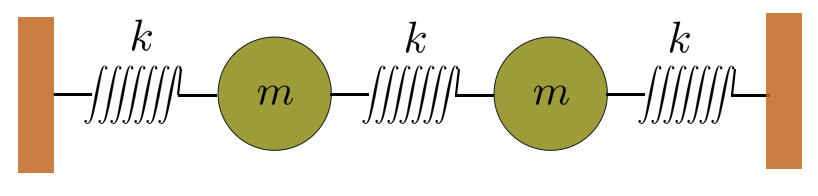
\includegraphics[width=2.3in]{VOLUMEN_1/04_Auto_Vectores/Figuras/Figura4_1.jpg}
\end{minipage}
\end{figure}
%%%%%%%%%%%%%%%%%

Podremos expresar estas ecuaciones en forma de operadores:
\[
\mathbb{D}\left| {x} \right>=0 \quad \Leftrightarrow \quad 
\left(\begin{array}{cc}m\frac{d^2}{dt^2} +2k & -k \\ -k & m\frac{d^2}{dt^2} +2k\end{array}\right) \left(\begin{array}{c}x^{1} \\x^{2}\end{array}\right) = 0 \,.
\]

Si pensamos esta ecuaci�n como una ecuaci�n de autovalores, el autovalor es claramente $\lambda = 0$, y como las masas y las constantes el�sticas son iguales podemos intercambiar las part�culas y la f�sica (las ecuaciones de movimiento) no cambian. Esto se puede expresar matem�ticamente como el operador permutaci�n de las part�culas:
\[
\mathbb{P}=\left(\begin{array}{cc}0 & 1 \\1 & 0 \end{array}\right) 
\quad \Rightarrow \quad 
\left(\begin{array}{cc}0 & 1 \\1 & 0 \end{array}\right) \left(\begin{array}{c}x^{1} \\x^{2}\end{array}\right) = \left(\begin{array}{c}x^{2} \\x^{1}\end{array}\right) \,.
\]

Es inmediato comprobar que $\left[ \mathbb{D},\mathbb{P} \right]=0$, con lo cual existir� una combinaci�n lineal de autovectores de $\mathbb{D}$ (asociados con el autovalor $\lambda = 0$) los cuales tambi�n ser�n autovectores de $\mathbb{P}$. Para ello procedamos a calcular los autovalores y autovectores de $\mathbb{P}$:
\[
\mathbb{P}\left| {x} \right>=\lambda\left| {x} \right> 
\,\, \Rightarrow \,\, 
\left|\begin{array}{cc}-\lambda & 1 \\1 & -\lambda\end{array}\right| =0 
\,\, \Rightarrow \,\,   \lambda\pm 1 \,\, \Leftrightarrow \,\, \left| \hat{\mathrm{e}}_{1} \right>= \frac{1}{\sqrt{2}}\left( \begin{array}{c} 1 \\1\end{array}\right); \quad \left| \hat{\mathrm{e}}_{2} \right>= \frac{1}{\sqrt{2}}\left(\begin{array}{c}1 \\-1\end{array}\right)\,.
\]

F�cilmente podemos expresar el vector posici�n como una combinaci�n lineal de estos dos autovectores de $\mathbb{P}$,  esto es:
\[
\left(\begin{array}{c}x^{1} \\x^{2}\end{array}\right) = \frac{\xi_{1}}{\sqrt{2}}\left( \begin{array}{c} 1 \\1\end{array}\right) + \frac{\xi_{2}}{\sqrt{2}}\left(\begin{array}{c}1 \\-1\end{array}\right) 
\,\, \Rightarrow \,\, 
\left\{\begin{array}{c}\xi_{1} =\frac{1}{\sqrt{2}}\left( x_{1}+x_{2} \right) \\ \\\xi_{2} =\frac{1}{\sqrt{2}}\left( x_{1}-x_{2} \right)\end{array}\right.
\]

Es claro que 
\[
\left| {u}_{1} \right>= \frac{1}{\sqrt{2}}\left( x_{1}+x_{2} \right)\left( \begin{array}{c} 1 \\1\end{array}\right)  \qquad \text{y} \qquad \left| {u}_{2} \right>= \frac{1}{\sqrt{2}}\left( x_{1}-x_{2} \right)\left(\begin{array}{r}1 \\-1\end{array}\right)\,,
\]
son autovectores de $\mathbb{P}$ y $\mathbb{D}$.

\item  Un operador cantidad de movimiento generalizado se define como aquel conjunto de operadores herm�ticos que cumplen con:
\[
\left[  \mathbb{J}_{x},\mathbb{J}_{y}\right]  =i\hbar\mathbb{J}_{z}\,, \quad 
\left[  \mathbb{J}_{y},\mathbb{J}_{z}\right]  =i\hbar\mathbb{J}_{x}\,, \quad 
\left[  \mathbb{J}_{z},\mathbb{J}_{x}\right]  =i\hbar\mathbb{J}_{y}\,, \quad \text{es decir:} \quad \left[  \mathbb{J}_{i},\mathbb{J}_{j}\right] = i\hbar\epsilon_{ijk}\mathbb{J}_{k} \,,
\]
con $\epsilon_{ijk}$ el s�mbolo de Levy-Civita (Aqu� los �ndices repetidos NO indican suma). 

Adicionalmente, definimos los siguientes operadores:
\[
\mathbb{J}^{2}=\mathbb{J}_{x}^{2}+\mathbb{J}_{y}^{2}+\mathbb{J}_{z}^{2}\,, \,\,\,
\mathbb{J}_{+}=\mathbb{J}_{x}+i\mathbb{J}_{y} \,, \,\,\,
\mathbb{J}_{-}=\mathbb{J}_{x}-i\mathbb{J}_{y}\,.
\]

Queremos demostrar que:
\[
\left[  \mathbb{J}^{2},\mathbb{J}_{+}\right] =\left[  \mathbb{J}^{2},\mathbb{J}_{-}\right]  =\left[  \mathbb{J}^{2},\mathbb{J}_{z}\right] =0 \,.
\]

Para probar esta propiedad se puede demostrar de forma gen�rica que  $\left[  \mathbb{J}^{2}_{k},\mathbb{J}_{m}\right] =0$, con $k,m = 1,2,3 \equiv x,y,z$, esto es:
  \[
  \left[  \mathbb{J}^{2}_{k},\mathbb{J}_{m}\right] = \left[  \mathbb{J}_{k}\mathbb{J}_{k},\mathbb{J}_{m}\right] =  \mathbb{J}_{k}\mathbb{J}_{k} \mathbb{J}_{m} - \mathbb{J}_{m} \mathbb{J}_{k}  \mathbb{J}_{k} =
   \mathbb{J}_{k}\mathbb{J}_{k} \mathbb{J}_{m}  - \left(  i\hbar\epsilon_{mkl}\mathbb{J}_{l} + \mathbb{J}_{k} \mathbb{J}_{m} \right) \mathbb{J}_{k}\,,
  \]
  con lo cual:
  \[
  \left[  \mathbb{J}^{2}_{k},\mathbb{J}_{m}\right] = \mathbb{J}_{k}\mathbb{J}_{k} \mathbb{J}_{m}  -  i\hbar\epsilon_{mkl}\mathbb{J}_{l}\mathbb{J}_{k} - \mathbb{J}_{k} \left(  i\hbar\epsilon_{mkn}\mathbb{J}_{n} + \mathbb{J}_{k} \mathbb{J}_{m} \right)\,,
   \] 
y claramente se anula por cuanto los �ndices no suman pero si son mudos, y $\epsilon_{mkl} = - \epsilon_{mlk}$.
\[
\left[  \mathbb{J}^{2}_{k},\mathbb{J}_{m}\right]=\mathbb{J}_{k}\mathbb{J}_{k} \mathbb{J}_{m}  -  
i\hbar\epsilon_{mkl}\mathbb{J}_{l}\mathbb{J}_{k} -  i\hbar\epsilon_{mkn}\mathbb{J}_{k}  \mathbb{J}_{n} -\mathbb{J}_{k}  \mathbb{J}_{k} \mathbb{J}_{m}\,,
   \]
al conmutar los cuadrados de las componentes con cualquiera de las componentes, y dado que los conmutadores son lineales entonces queda demostrado que: 
   \[
 \left[  \mathbb{J}^{2},\mathbb{J}_{\pm}\right] =   \left[ \mathbb{J}_{x}^{2}+\mathbb{J}_{y}^{2}+\mathbb{J}_{z}^{2},\mathbb{J}_{x} \pm i\mathbb{J}_{y} \right] = \left[ \mathbb{J}_{y}^{2},\mathbb{J}_{x} \right] + \left[ \mathbb{J}_{z}^{2},\mathbb{J}_{x}  \right] \pm i \left[ \mathbb{J}_{x}^{2}, \mathbb{J}_{y} \right]  \pm i \left[ \mathbb{J}_{z}^{2},\mathbb{J}_{y} \right] =0\,.
   \]
   
 \item Si definimos los autovectores comunes a $\mathbb{J}^{2}$ y
$\mathbb{J}_{z}$ como $\left|  j,m\right\rangle $ de la siguiente manera:
\[
\mathbb{J}^{2}\left|  j,m\right\rangle   =j\left(  j+1\right)  \hbar^{2}\left|  j,m\right\rangle\,, \quad
\mathbb{J}_{z}\left|  j,m\right\rangle   =m\hbar \left|  j,m\right\rangle\,, \quad \text{con: }
\left\langle  j,m\right. \left|  j',m' \right\rangle = \delta_{jj'}\delta_{mm'} \,,
\]
y adicionalmente tenemos que:
\[
\mathbb{J}_{-}\left|  j,m\right\rangle  = \hbar\sqrt{j(j+1)  - m(  m-1)  }\left|  j,m-1\right\rangle \,, \quad
\mathbb{J}_{+}\left|  j,m\right\rangle  = \hbar\sqrt{j (j+1)  - m (  m+1)  }\left|  j,m+1\right\rangle.          
\]

Si se supone (es f�cil demostrarlo) que $-j\leq m\leq j$. Esto quiere decir que dado
alg�n valor  $j$, $m$ var�an entre $-j$ y $j$ de uno en uno, esto es: 
$m=-j,-j+1,-j+2,\cdots,j-2,j-1,j$. Supongamos ahora que $j=\frac{1}{2}$.  

Busquemos:
\begin{enumerate}
\item La representaci�n matricial para:  $\mathbb{J}_{z},\mathbb{J}_{-},\mathbb{J}_{+}, \mathbb{J}^2$, en la base de autovectores de $\mathbb{J}_{z}$ y $\mathbb{J}^2$.

Si $\left|  j,m\right\rangle $ son autovectores de  $\mathbb{J}^{2}$ y $\mathbb{J}_{z}$ su representaci�n matricial  ser� diagonal y como $m$ var�a entre  $-j$ y $j$ con incrementos de $1$ tendremos que ser�n matrices $2\times2$. La base ortogonal de autovectores ser�: $\big\{ \left|  \frac{1}{2},-\frac{1}{2}\right\rangle,\left|  \frac{1}{2}, \frac{1}{2}\right\rangle \big\}$.
  \[
  \left(\begin{array}{cc}
  \left\langle \frac{1}{2},\frac{1}{2}\right| \mathbb{J}_{z} \left|  \frac{1}{2},\frac{1}{2}\right\rangle  & 
  \left\langle \frac{1}{2},\frac{1}{2}\right| \mathbb{J}_{z} \left|  \frac{1}{2},-\frac{1}{2}\right\rangle    \\ \\
    \left\langle \frac{1}{2},-\frac{1}{2}\right| \mathbb{J}_{z} \left|  \frac{1}{2},\frac{1}{2}\right\rangle   & 
       \left\langle \frac{1}{2},-\frac{1}{2}\right| \mathbb{J}_{z} \left|  \frac{1}{2},-\frac{1}{2}\right\rangle 
\end{array}
  \right) \equiv
  \dfrac{\hbar}{2}  \left(\begin{array}{cc}
   1 &  0   \\ \\
  0   & -1 
\end{array}
  \right) \,,
  \]
  \[
  \left(\begin{array}{cc}
  \left\langle \frac{1}{2},\frac{1}{2}\right| \mathbb{J}^{2} \left|  \frac{1}{2},\frac{1}{2}\right\rangle  & 
  \left\langle \frac{1}{2},\frac{1}{2}\right| \mathbb{J}^{2} \left|  \frac{1}{2},-\frac{1}{2}\right\rangle    \\ \\
    \left\langle \frac{1}{2},-\frac{1}{2}\right| \mathbb{J}^{2} \left|  \frac{1}{2},\frac{1}{2}\right\rangle   & 
       \left\langle \frac{1}{2},-\frac{1}{2}\right| \mathbb{J}^{2} \left|  \frac{1}{2},-\frac{1}{2}\right\rangle 
\end{array}
  \right) \equiv
   \dfrac{3}{4}\hbar^{2} \left(\begin{array}{cc}
  1  &  0   \\ \\
     0   & 1 
\end{array}
  \right) \,.
  \]  
  
La representaci�n matricial para $\mathbb{J}_{-},\mathbb{J}_{+}$ obviamente no ser� diagonal:
    \[
  \left(\begin{array}{cc}
  \left\langle \frac{1}{2},\frac{1}{2}\right| \mathbb{J}_{+} \left|  \frac{1}{2},\frac{1}{2}\right\rangle  & 
  \left\langle \frac{1}{2},\frac{1}{2}\right| \mathbb{J}_{+} \left|  \frac{1}{2},-\frac{1}{2}\right\rangle    \\ \\
    \left\langle \frac{1}{2},-\frac{1}{2}\right| \mathbb{J}_{+} \left|  \frac{1}{2},\frac{1}{2}\right\rangle   & 
       \left\langle \frac{1}{2},-\frac{1}{2}\right| \mathbb{J}_{+} \left|  \frac{1}{2},-\frac{1}{2}\right\rangle 
\end{array}
  \right) \equiv
  \hbar \left(\begin{array}{cc}
   0  &  1   \\ \\
  0  & 0 
\end{array}
  \right)\,,
  \]
   \[
  \left(\begin{array}{cc}
  \left\langle \frac{1}{2},\frac{1}{2}\right| \mathbb{J}_{-} \left|  \frac{1}{2},\frac{1}{2}\right\rangle  & 
  \left\langle \frac{1}{2},\frac{1}{2}\right| \mathbb{J}_{-} \left|  \frac{1}{2},-\frac{1}{2}\right\rangle    \\ \\
    \left\langle \frac{1}{2},-\frac{1}{2}\right| \mathbb{J}_{-} \left|  \frac{1}{2},\frac{1}{2}\right\rangle   & 
       \left\langle \frac{1}{2},-\frac{1}{2}\right| \mathbb{J}_{-} \left|  \frac{1}{2},- \frac{1}{2}\right\rangle 
\end{array}
  \right) \equiv
    \hbar  \left(\begin{array}{cc}
   0 &  0   \\ \\
1  & 0
\end{array}
  \right)\,.
  \]

 \item Calculemos los autovalores y autovalores para: $ \mathbb{J}_{z},  \mathbb{J}_{-},\mathbb{J}_{+}, \mathbb{J}^2$.

Otra vez, $\big\{ \left|  \frac{1}{2},-\frac{1}{2}\right\rangle,\left|  \frac{1}{2}, \frac{1}{2}\right\rangle \big\}$ son autovectores de  $\mathbb{J}^{2}$ y $\mathbb{J}_{z}$. En el caso de $\mathbb{J}^{2}$  con un autovalor de $ \frac{3}{4}\hbar^{2}$ para ambos autovectores y en el caso de $\mathbb{J}_{z}$ los autovalores ser�n $\pm  \frac{\hbar}{2} $ respectivamente. Para $ \mathbb{J}_{-},\mathbb{J}_{+}$ no tendr�n autovalor distinto de cero en esta base.
\end{enumerate} 
\end{enumerate}

\newpage
\subsection{{\color{red}Practicando con Maxima}} 

Consideremos uno de los ejemplos anteriores donde:

%%%%%% INPUT:
\begin{minipage}[t]{8ex}
{\color{red}\bf \begin{verbatim} (%i1) 
\end{verbatim}}
\end{minipage}
\begin{minipage}[t]{\textwidth}{\color{blue}
\begin{verbatim}
A:matrix([1,0,3], [0,-2,0], [3,0,1]);
\end{verbatim}}
\end{minipage}

%%% OUTPUT:
\begin{math}\displaystyle \parbox{8ex}{\color{labelcolor}(\%o1) }
\begin{pmatrix}1 & 0 & 3 \\ 0 & -2 & 0 \\ 3 & 0 & 1 \\ 
 \end{pmatrix}
\end{math}

%%%%%% INPUT:
\begin{minipage}[t]{8ex}
{\color{red}\bf \begin{verbatim} (%i2) 
\end{verbatim}}
\end{minipage}
\begin{minipage}[t]{\textwidth}{\color{blue}
\begin{verbatim}
eigenvectors(A);
\end{verbatim}}
\end{minipage}

%%% OUTPUT:
\begin{math}\displaystyle \parbox{8ex}{\color{labelcolor}(\%o2) }
\left[ \left[ \left[ -2 , 4 \right]  , \left[ 2 , 1 \right] 
  \right]  , \left[ \left[ \left[ 1 , 0 , -1 \right]  , \left[ 0 , 1
  , 0 \right]  \right]  , \left[ \left[ 1 , 0 , 1 \right]  \right] 
  \right]  \right] 
\end{math}
\newline

El resultado es una lista con los autovalores y su multiplicidad, y para cada autovalor los autovectores como sublistas. Es necesario manipular estas sublistas para obtener los autovectores. Entonces, es mejor escribir:

%%%%%% INPUT:
\begin{minipage}[t]{8ex}
{\color{red}\bf \begin{verbatim} (%i3) 
\end{verbatim}}
\end{minipage}
\begin{minipage}[t]{\textwidth}{\color{blue}
\begin{verbatim}
[val,vec]:eigenvectors(A);
\end{verbatim}}
\end{minipage}

%%% OUTPUT:
\begin{math}\displaystyle \parbox{8ex}{\color{labelcolor}(\%o3) }
\left[ \left[ \left[ -2 , 4 \right]  , \left[ 2 , 1 \right]   \right]  , \left[ \left[ \left[ 1 , 0 , -1 \right]  , \left[ 0 , 1 , 0 \right]  \right]  , \left[ \left[ 1 , 0 , 1 \right]  \right]  \right]  \right] 
\end{math}
\newline

Por lo tanto, una lista con los autovalores es la siguiente:

%%%%%% INPUT:
\begin{minipage}[t]{8ex}
{\color{red}\bf \begin{verbatim} (%i4) 
\end{verbatim}}
\end{minipage}
\begin{minipage}[t]{\textwidth}{\color{blue}
\begin{verbatim}
autovalores:val[1];
\end{verbatim}}
\end{minipage}

%%% OUTPUT:
\begin{math}\displaystyle \parbox{8ex}{\color{labelcolor}(\%o4) }
\left[ -2 , 4 \right]
 \end{math}
\newline
 
Notemos el orden: los dos primeros vectores corresponden al autovalor $-2$ y el tercero al autovalor $4$. 

Los autovectores como listas son:

%%%%%% INPUT:
\begin{minipage}[t]{8ex}
{\color{red}\bf \begin{verbatim} (%i5) 
\end{verbatim}}
\end{minipage}
\begin{minipage}[t]{\textwidth}{\color{blue}
\begin{verbatim}
L1:vec[1];L2:vec[2];
\end{verbatim}}
\end{minipage}

%%% OUTPUT:
\begin{math}\displaystyle \parbox{8ex}{\color{labelcolor}(\%o5) }
\left[ \left[ 1 , 0 , -1 \right]  , \left[ 0 , 1 , 0 \right]   \right] 
 \end{math}
 
 %%% OUTPUT:
\begin{math}\displaystyle \parbox{8ex}{\color{labelcolor}(\%o5) }
\left[ \left[ 1 , 0 , 1 \right]  \right] 
 \end{math}
\newline

Pero resulta conveniente separar cada autovector.

%%%%%% INPUT:
\begin{minipage}[t]{8ex}
{\color{red}\bf \begin{verbatim} (%i6) 
\end{verbatim}}
\end{minipage}
\begin{minipage}[t]{\textwidth}{\color{blue}
\begin{verbatim}
L1[1];L1[2];L2[1];
\end{verbatim}}
\end{minipage}

%%% OUTPUT:
\begin{math}\displaystyle \parbox{8ex}{\color{labelcolor}(\%o6) }
\left[ 1 , 0 , -1 \right] 
 \end{math}
 
%%% OUTPUT:
\begin{math}\displaystyle \parbox{8ex}{\color{labelcolor}(\%o7) }
\left[ 0 , 1 , 0 \right]
 \end{math}
 
 %%% OUTPUT:
\begin{math}\displaystyle \parbox{8ex}{\color{labelcolor}(\%o8) }
\left[ 1 , 0 , 1 \right] 
 \end{math}
\newline
 
Vamos ahora a normalizar los autovectores:

 %%%%%% INPUT:
\begin{minipage}[t]{8ex}
{\color{red}\bf \begin{verbatim} (%i9) 
\end{verbatim}}
\end{minipage}
\begin{minipage}[t]{\textwidth}{\color{blue}
\begin{verbatim}
V1:L1[1]/sqrt(L1[1].L1[1]);V2:L1[2]/sqrt(L1[2].L1[2]);V3:L2[1]/sqrt(L2[1].L2[1]);
\end{verbatim}}
\end{minipage}

%%% OUTPUT:
\begin{math}\displaystyle \parbox{8ex}{\color{labelcolor}(\%o9) }
\left[ \frac{1}{\sqrt{2}} , 0 , -\frac{1}{\sqrt{2}} \right] 
 \end{math}
 
 %%% OUTPUT:
\begin{math}\displaystyle \parbox{8ex}{\color{labelcolor}(\%o10) }
\left[ 0 , 1 , 0 \right] 
 \end{math}
 
 %%% OUTPUT:
\begin{math}\displaystyle \parbox{8ex}{\color{labelcolor}(\%o11) }
\left[ \frac{1}{\sqrt{2}} , 0 , \frac{1}{\sqrt{2}} \right]
 \end{math}
\newline

Hacemos una lista con los vectores normalizados:

 %%%%%% INPUT:
\begin{minipage}[t]{8ex}
{\color{red}\bf \begin{verbatim} (%i12) 
\end{verbatim}}
\end{minipage}
\begin{minipage}[t]{\textwidth}{\color{blue}
\begin{verbatim}
Lvec:[V1,V2,V3];
\end{verbatim}}
\end{minipage}

%%% OUTPUT:
\begin{math}\displaystyle \parbox{8ex}{\color{labelcolor}(\%o12) }
\left[ \left[ \frac{1}{\sqrt{2}} , 0 , -\frac{1}{\sqrt{2}} \right] 
, \left[ 0 , 1 , 0 \right]  , \left[ \frac{1}{\sqrt{2}} , 0 , 
 \frac{1}{\sqrt{2}} \right]  \right] 
 \end{math}
\newline

Y construimos la matriz $ \mathbb{C}$:

 %%%%%% INPUT:
\begin{minipage}[t]{8ex}
{\color{red}\bf \begin{verbatim} (%i13) 
\end{verbatim}}
\end{minipage}
\begin{minipage}[t]{\textwidth}{\color{blue}
\begin{verbatim}
C:transpose(apply('matrix,Lvec));
\end{verbatim}}
\end{minipage}

%%% OUTPUT:
\begin{math}\displaystyle \parbox{8ex}{\color{labelcolor}(\%o13) }
\begin{pmatrix}\frac{1}{\sqrt{2}} & 0 & \frac{1}{\sqrt{2}} \\ 0 & 1
  & 0 \\ -\frac{1}{\sqrt{2}} & 0 & \frac{1}{\sqrt{2}} \\ 
 \end{pmatrix}
 \end{math}
\newline

Para finalmente comprobar:

 %%%%%% INPUT:
\begin{minipage}[t]{8ex}
{\color{red}\bf \begin{verbatim} (%i14) 
\end{verbatim}}
\end{minipage}
\begin{minipage}[t]{\textwidth}{\color{blue}
\begin{verbatim}
transpose(C).A.C;
\end{verbatim}}
\end{minipage}

%%% OUTPUT:
\begin{math}\displaystyle \parbox{8ex}{\color{labelcolor}(\%o14) }
\begin{pmatrix}-2 & 0 & 0 \\ 0 & -2 & 0 \\ 0 & 0 & 4 \\ 
 \end{pmatrix}
 \end{math}
\newline

Consideremos ahora otro de los ejemplos, donde ten�amos la siguiente matriz:

%%%%%% INPUT:
\begin{minipage}[t]{8ex}
{\color{red}\bf \begin{verbatim} (%i15) 
\end{verbatim}}
\end{minipage}
\begin{minipage}[t]{\textwidth}{\color{blue}
\begin{verbatim}
A:matrix([1,-1+2*%i,%i],[-1-2*%i,2,-1],[-%i,-1,3]);
\end{verbatim}}
\end{minipage}

%%% OUTPUT:
\begin{math}\displaystyle \parbox{8ex}{\color{labelcolor}(\%o15) }
\begin{pmatrix}1 & 2\,i-1 & i \\ -2\,i-1 & 2 & -1 \\ -i & -1 & 3 \\ \end{pmatrix}
 \end{math}
\newline

Es f�cil ver que se trata de una matriz herm�tica

%%%%%% INPUT:
\begin{minipage}[t]{8ex}
{\color{red}\bf \begin{verbatim} (%i16) 
\end{verbatim}}
\end{minipage}
\begin{minipage}[t]{\textwidth}{\color{blue}
\begin{verbatim}
transpose(conjugate(A))=A;
\end{verbatim}}
\end{minipage}

%%% OUTPUT:
\begin{math}\displaystyle \parbox{8ex}{\color{labelcolor}(\%o16) }
\begin{pmatrix}1 & 2\,i-1 & i \\ -2\,i-1 & 2 & -1 \\ -i & -1 & 3 \\ \end{pmatrix}=\begin{pmatrix}1 & 2\,i-1 & i \\ -2\,i-1 & 2 & -1 \\ 
-i & -1 & 3 \\ \end{pmatrix}
 \end{math}
\newline

Calculamos los autovalores y autovectores:

%%%%%% INPUT:
\begin{minipage}[t]{8ex}
{\color{red}\bf \begin{verbatim} (%i17) 
\end{verbatim}}
\end{minipage}
\begin{minipage}[t]{\textwidth}{\color{blue}
\begin{verbatim}
[val,vec]:eigenvectors(A)$
\end{verbatim}}
\end{minipage}
\newline

Al primer elemento de la lista, le asignaremos la variable {\tt autovalores}, como se muestra a continuaci�n:

%%%%%% INPUT:
\begin{minipage}[t]{8ex}
{\color{red}\bf \begin{verbatim} (%i18) 
\end{verbatim}}
\end{minipage}
\begin{minipage}[t]{\textwidth}{\color{blue}
\begin{verbatim}
autovalores:val[1];
\end{verbatim}}
\end{minipage}

%%% OUTPUT:
\begin{math}\displaystyle \parbox{8ex}{\color{labelcolor}(\%o18) }
\left[ 1-\sqrt{5} , \sqrt{5}+1 , 4 \right] 
 \end{math}
\newline

Ahora procedemos a aislar los diferentes autovectores, es importante tener en mente el orden para utilizar las etiquetas apropiadas.

%%%%%% INPUT:
\begin{minipage}[t]{8ex}
{\color{red}\bf \begin{verbatim} (%i19) 
\end{verbatim}}
\end{minipage}
\begin{minipage}[t]{\textwidth}{\color{blue}
\begin{verbatim}
L1:vec[1]$L1[1]; L2:vec[2]$L2[1]; L3:vec[3]$L3[1];
\end{verbatim}}
\end{minipage}

%%% OUTPUT:
\begin{math}\displaystyle \parbox{8ex}{\color{labelcolor}(\%o20) }
\left[ 1 , \frac{\sqrt{5}\,i+1}{3} , \frac{\left(\sqrt{5}-1\right)
 \,i+\sqrt{5}-2}{3} \right] 
 \end{math}

%%% OUTPUT:
\begin{math}\displaystyle \parbox{8ex}{\color{labelcolor}(\%o22) }
\left[ 1 , -\frac{\sqrt{5}\,i-1}{3} , -\frac{\left(\sqrt{5}+1 \right)\,i+\sqrt{5}+2}{3} \right] 
 \end{math}
 
 %%% OUTPUT:
\begin{math}\displaystyle \parbox{8ex}{\color{labelcolor}(\%o24) }
\left[ 1 , -i-1 , 1 \right]
 \end{math}
 \newline
 
Los autovectores normalizados son:
 
%%%%%% INPUT:
\begin{minipage}[t]{8ex}
{\color{red}\bf \begin{verbatim} (%i25) 
\end{verbatim}}
\end{minipage}
\begin{minipage}[t]{\textwidth}{\color{blue}
\begin{verbatim}
u1:L1[1]/sqrt(L1[1].L1[1]),ratsimp;
\end{verbatim}}
\end{minipage}

%%% OUTPUT:
\begin{math}\displaystyle \parbox{8ex}{\color{labelcolor}(\%o25) }
\left[ \frac{3}{\sqrt{-\left(4\,\sqrt{5}-14\right)\,i-2\,\sqrt{5}+8
 }} , \frac{\sqrt{5}\,i+1}{\sqrt{-\left(4\,\sqrt{5}-14\right)\,i-2\,
 \sqrt{5}+8}} , \frac{\left(\sqrt{5}-1\right)\,i+\sqrt{5}-2}{\sqrt{-
 \left(4\,\sqrt{5}-14\right)\,i-2\,\sqrt{5}+8}} \right] 
 \end{math}

%%%%%% INPUT:
\begin{minipage}[t]{8ex}
{\color{red}\bf \begin{verbatim} (%i26) 
\end{verbatim}}
\end{minipage}
\begin{minipage}[t]{\textwidth}{\color{blue}
\begin{verbatim}
u2:L2[1]/sqrt(L2[1].L2[1]),ratsimp;
\end{verbatim}}
\end{minipage}

%%% OUTPUT:
\begin{math}\displaystyle \parbox{8ex}{\color{labelcolor}(\%o26) }
\left[ \frac{3}{\sqrt{\left(4\,\sqrt{5}+14\right)\,i+2\,\sqrt{5}+8}
 } , -\frac{\sqrt{5}\,i-1}{\sqrt{\left(4\,\sqrt{5}+14\right)\,i+2\,
 \sqrt{5}+8}} , -\frac{\left(\sqrt{5}+1\right)\,i+\sqrt{5}+2}{\sqrt{
 \left(4\,\sqrt{5}+14\right)\,i+2\,\sqrt{5}+8}} \right] 
 \end{math}
 
 %%%%%% INPUT:
\begin{minipage}[t]{8ex}
{\color{red}\bf \begin{verbatim} (%i27) 
\end{verbatim}}
\end{minipage}
\begin{minipage}[t]{\textwidth}{\color{blue}
\begin{verbatim}
u3:L3[1]/sqrt(L3[1].L3[1]),ratsimp;
\end{verbatim}}
\end{minipage}

%%% OUTPUT:
\begin{math}\displaystyle \parbox{8ex}{\color{labelcolor}(\%o27) }
\left[ \frac{1}{\sqrt{2\,i+2}} , -\frac{i+1}{\sqrt{2\,i+2}} , 
 \frac{1}{\sqrt{2\,i+2}} \right] 
 \end{math}
\newline

Estos vectores ser�n ortogonales, como podemos ver:

%%%%%% INPUT:
\begin{minipage}[t]{8ex}
{\color{red}\bf \begin{verbatim} (%i28) 
\end{verbatim}}
\end{minipage}
\begin{minipage}[t]{\textwidth}{\color{blue}
\begin{verbatim}
conjugate(u1).u2,ratsimp;conjugate(u1).u3,ratsimp;conjugate(u3).u2,ratsimp;
\end{verbatim}}
\end{minipage}

%%% OUTPUT:
\begin{math}\displaystyle \parbox{8ex}{\color{labelcolor}(\%o28) }
0
\end{math}

%%% OUTPUT:
\begin{math}\displaystyle \parbox{8ex}{\color{labelcolor}(\%o29) }
0
\end{math}
 
 %%% OUTPUT:
\begin{math}\displaystyle \parbox{8ex}{\color{labelcolor}(\%o30) }
0
\end{math}
\newline

Para construir la matriz  $C$ preparamos primero el siguiente arreglo:

%%%%%% INPUT:
\begin{minipage}[t]{8ex}
{\color{red}\bf \begin{verbatim} (%i31) 
\end{verbatim}}
\end{minipage}
\begin{minipage}[t]{\textwidth}{\color{blue}
\begin{verbatim}
Lvec:[u1,u2,u3]$
\end{verbatim}}
\end{minipage}
\newline

Con cada autovector como columna construimos la matriz $C$:

%%%%%% INPUT:
\begin{minipage}[t]{8ex}
{\color{red}\bf \begin{verbatim} (%i32) 
\end{verbatim}}
\end{minipage}
\begin{minipage}[t]{\textwidth}{\color{blue}
\begin{verbatim}
C:transpose(apply('matrix,Lvec));
\end{verbatim}}
\end{minipage}

%%% OUTPUT:
\begin{math}\displaystyle \parbox{8ex}{\color{labelcolor}(\%o32) }
\begin{pmatrix}\frac{3}{\sqrt{-\left(4\,\sqrt{5}-14\right)\,i-2\,
 \sqrt{5}+8}} & \frac{3}{\sqrt{\left(4\,\sqrt{5}+14\right)\,i+2\,
 \sqrt{5}+8}} & \frac{1}{\sqrt{2\,i+2}} \\ \frac{\sqrt{5}\,i+1}{
 \sqrt{-\left(4\,\sqrt{5}-14\right)\,i-2\,\sqrt{5}+8}} & -\frac{
 \sqrt{5}\,i-1}{\sqrt{\left(4\,\sqrt{5}+14\right)\,i+2\,\sqrt{5}+8}}
  & -\frac{i+1}{\sqrt{2\,i+2}} \\ \frac{\left(\sqrt{5}-1\right)\,i+
 \sqrt{5}-2}{\sqrt{-\left(4\,\sqrt{5}-14\right)\,i-2\,\sqrt{5}+8}} & 
 -\frac{\left(\sqrt{5}+1\right)\,i+\sqrt{5}+2}{\sqrt{\left(4\,\sqrt{5
 }+14\right)\,i+2\,\sqrt{5}+8}} & \frac{1}{\sqrt{2\,i+2}} \\ 
 \end{pmatrix}
\end{math}
\newline

La inversa de la matriz $C$ se obtiene como ya sabemos:

%%%%%% INPUT:
\begin{minipage}[t]{8ex}
{\color{red}\bf \begin{verbatim} (%i33) 
\end{verbatim}}
\end{minipage}
\begin{minipage}[t]{\textwidth}{\color{blue}
\begin{verbatim}
Cinv:invert(C),ratsimp$
\end{verbatim}}
\end{minipage}
\newline

Aqu� aplicamos una rutina de simplificaci�n a cada uno de los elementos de la matriz. Esto lo hicimos con el comando {\tt ratsimp}. 

Para finalmente poder calcular $C^{-1} A C$ y obtener:

%%%%%% INPUT:
\begin{minipage}[t]{8ex}
{\color{red}\bf \begin{verbatim} (%i34) 
\end{verbatim}}
\end{minipage}
\begin{minipage}[t]{\textwidth}{\color{blue}
\begin{verbatim}
Cinv.A.C,ratsimp;
\end{verbatim}}
\end{minipage}

%%% OUTPUT:
\begin{math}\displaystyle \parbox{8ex}{\color{labelcolor}(\%o34) }
\begin{pmatrix}\frac{\sqrt{5}-5}{\sqrt{5}} & 0 & 0 \\ 0 & \frac{
 \sqrt{5}+5}{\sqrt{5}} & 0 \\ 0 & 0 & 4 \\ 
 \end{pmatrix}
\end{math}

\begin{center}
{\color{red}\rule{15.8cm}{0.4mm}}
\end{center}



\subsection{{\color{OliveGreen}Ejercicios}}
\begin{enumerate}
\item Encuentre los autovalores y autovectores de las matrices:
\[
 \mathbb{A}=
\left(
\begin{array}
[c]{cccc}
0 & -i & 0 & 0 \\
i & 0 & 0 & 0 \\
0 & 0 & 0 & -i \\
0 & 0& i & 0  
\end{array}
\right) \,,\quad 
 \mathbb{B}=
\left(
\begin{array}
[c]{cccc}
1 & 0 & 0 & 0 \\
0 & -1 & 0 & 0 \\
0 & 0 & 1 & 0 \\
0 & 0 & 0 & -1 
\end{array}
\right)
\]

\item Diagonalizar unitariamente: 
\[
 \mathbb{A}=
\left(
\begin{array}
[c]{cc}
2 & -i \\
i & 1 
\end{array}
\right) \,,\quad 
 \mathbb{B}=
\left(
\begin{array}
[c]{ccc}
1 & 1+i & 2i\\
1-i & 5 & -3\\
-2i & -3 & 0
\end{array}
\right)
\]


\item Diagonalizar ortogonalmente: 
\[
 \mathbb{A}=
\left(
\begin{array}
[c]{cc}
1 & -3 \\
-3 & 1 
\end{array}
\right) \,,\quad 
 \mathbb{B}=
\left(
\begin{array}
[c]{ccc}
3 & -2 & 4\\
-2 & 6 & 2\\
4 & 2 & 3
\end{array}
\right)
\]

\item Demuestre que la matriz
\[
 \mathbb{C}=
\left(
\begin{array}
[c]{cc}
x & x-iy \\
x+iy & -z 
\end{array}
\right)
\]
es igual a $ \mathbb{C}=x{\boldsymbol \sigma}_1+y{\boldsymbol \sigma}_2+z{\boldsymbol \sigma}_3$. Donde las matrices ${\boldsymbol \sigma}_i$ son la matrices de Pauli.

\item Las transformaciones de Lorentz se pueden escribir de manera matricial como
\[
\left(
\begin{array}
[c]{cccc}
\gamma & 0 & 0 & -i \gamma v /c \\
0 & 1 & 0 & 0\\
0 & 0 & 1 & 0\\
i \gamma v /c & 0 & 0 &  \gamma
\end{array}
\right)
\]
con $\gamma = (\sqrt{1-v^2/c^2})^{-1}$.  La matriz anterior �ser�  ortogonal? �ser� unitaria?

\item  Si los autovalores de una matriz herm�tica (o semi-herm�tica) $\mathbb{A}$ son todos iguales a $\lambda$, demuestre que $\mathbb{A} = \lambda \mathbb{I}$.

\item Si  una matriz $\mathbb{A}$ es semi-herm�tica, demuestre que $(\mathbb{I}-\mathbb{A})(\mathbb{I}+\mathbb{A})^{-1}$ es ortogonal.

\item Dado un observable $\mathbb{A}$ y un vector de estado $\left|\psi\right>$ general, definiremos el valor esperado de $\mathbb{A}$ a la cantidad $\left< \mathbb{A}\right> = \left<\psi\right| \mathbb{A}\left|\psi\right> $, y la relaci�n de dispersi�n de $\mathbb{A}$ como:
\[
\left< \left(\Delta\mathbb{A} \right)^{2} \right>  = 
\left< \left(\mathbb{A} - \left< \mathbb{A}\right> \mathbb{I} \right)^{2} \right> =
\left< \mathbb{A}^{2}\right> - \left< \mathbb{A}\right>^{2} \equiv 
\left<\psi\right| \mathbb{A}^{2}\left|\psi\right> -\left<\psi\right| \mathbb{A}\left|\psi\right>^{2} \,,
\] 
donde $\mathbb{I}$ es el operador identidad. N�tese que el valor esperado es un n�mero que representa la dispersi�n de un observable y tiene la misma estructura e interpretaci�n de la varianza en estad�stica. 
\begin{enumerate}
  \item Muestre que la dispersi�n siempre es positiva, i.e $\left< \left(\Delta\mathbb{A} \right)^{2} \right> \geqslant 0$. Para ello: 
  \begin{enumerate}
  \item Inicie mostrando que para cualquier operador herm�tico $\mathbb{C}$ se cumple $\left< \mathbb{C}^{2} \right> \geqslant 0$.
  \item Termine mostrando que $\mathbb{A} - \left< \mathbb{A}\right> \mathbb{I}$ es un operador herm�tico.
\end{enumerate}

  \item Muestre que la dispersi�n se anula para el caso en que $\left|\psi\right>$ es autovector de $\mathbb{A}$ con autovalor $\left< \mathbb{A}\right>$.
  
  \item Utilizando la desigualdad de Cauchy-Schwarz muestre que las relaciones de dispersi�n entre dos observables 
  $\mathbb{A}$ y $\mathbb{B}$ siempre cumplen con: 
  \[
\left< \left(\Delta\mathbb{A} \right)^{2} \right> \left< \left(\Delta\mathbb{B} \right)^{2} \right> \geqslant 
\frac{1}{4} \left| \left< [\mathbb{A}, \mathbb{B}]\right> \right|^{2} \quad \mathrm{con} \quad
[\mathbb{A}, \mathbb{B}] = \mathbb{A} \mathbb{B} -  \mathbb{B} \mathbb{A}\,.
\] 

Esta es la forma general de la relaci�n de incertidumbre.\footnote{Para detalles de las implicaciones de este problema se puede consultar Dumitru, S. ``On the uncertainty relations and quantum measurements: conventionalities, short comings, reconsideration. {\textrm arXiv preprint quant-ph/0504058 (2005)}. Y tambi�n  Dumitru, S. ``A possible general approach regarding the conformability of angular observables with mathematical rules of Quantum Mechanics. \textrm{arXiv preprint quant-ph/0602147} (2006).}

\item En Mec�nica Cu�ntica se define el operador de spin como $\mathbb{S}_{i} = \frac{\hbar}{2}\mathbf{\sigma}_{i} $, donde  las $\mathbf{\sigma}_{i}$ son las matrices de Pauli y los valores de  
 $i = 1,2,3$ representan las direcciones $x,y,z$, respectivamente.
  \begin{enumerate} 
  \item Encuentre la expresi�n para el conmutador: $[\mathbb{S}_{i},\mathbb{S}_{j}]$, con $i,j = 1,2,3$. 
  \item Considere un vector de estado general $\left|\psi\right> = a\left|+\right> + b\left|-\right>$, donde $a$ y $b$ son n�meros complejos que cumplen con: $a^{2} + b^{2}=1$ y $\left\{\left|+\right>,\left|-\right>\right\}$ la base de autovectores de $\mathbb{S}_{z}$. Muestre que: 
 \[
\left< \left(\Delta\mathbb{S}_{z} \right)^{2} \right> \left< \left(\Delta\mathbb{S}_{x} \right)^{2} \right> \geqslant 
\hbar^{4} [\mathrm{Im}(ab^{*})]^{2} \,,
 \] 
con   $\mathrm{Im}(\circ)$ la parte imaginaria del argumento.
\end{enumerate} 
\end{enumerate}

\item Dada la matriz: 
\[
\left(
\begin{array}
[c]{ccccccccc}
0 & q & 0 & 0 & 0 & \cdots & 0 & 0 & 0 \\
2q & 2^2 & q & 0 & 0 & \cdots & 0 & 0 & 0\\
0 & q & 4(2^2) & q & 0 & \cdots & 0 & 0 & 0\\
\vdots & \vdots& \vdots & \vdots & \vdots & \vdots & \vdots & \vdots & \vdots\\
0 & 0 & 0 & 0 & 0 & \cdots & 4(N-3)^2 & q & 0\\
0 & 0 & 0 & 0 & 0 & \cdots & q & 4(N-2)^2 & q\\
0 & 0 & 0 & 0 & 0 & \cdots & 0 & q & 4(N-1)^2
\end{array}
\right)
\]
Encuentre los autovalores y autovectores cuando $q=1$  y $N=10$.

\item Realice los ejercicios anteriores utilizando el programa {\bf Maxima}. 


\end{enumerate}










\begin{thebibliography}{9}
\bibitem{ArfkenWeberWeber2000}  Arfken, G. B.,Weber, H., Weber, H.J. (2000) \textbf{Mathematical Methods for Physicists} 5ta Edici�n (Academic Press, Nueva York)

\bibitem{BorisenkoTarapov1968}  Borisenko, A.I, y Tarapov I.E. (1968) \textbf{Vector and Tensor Analisys} (Dover Publications Inc, Nueva York)

\bibitem{DennerykKrzywicki1995}  Dennery, P. y Krzywicki, A. (1995) \textbf{Mathematics for Physicists} (Dover Publications Inc, Nueva York)

\bibitem{Harper1971}  Harper, C. (1971) \textbf{Introduction to Mathematical Physics} (\textit{Prentice Hall, Englewood Cliff, N.J:})

\bibitem{Hassani1991}  Hassani, S. (1991) \textbf{Foundations of Mathematical Physics} (\textit{Prentice Hall, International Edition, London:}

\bibitem{Hauser1971}  Hauser, W (1971) \textbf{Introduction to Principles of Electromagnetism }\ (\textit{Addison-Wesley Pub Co Reading})

\bibitem{RileyHobsonBence2002}  Riley, K.F., Hobson, M.P. y Bence, S.J. (2002) \textbf{Mathematical Methods for Physics and Engineering } (\textit{Cambridge University Press})

\bibitem{Santalo1969}  Santal�, L.A (1969) \textbf{Vectores y Tensores} (\textit{Editorial Universitaria, Buenos Aires})

\bibitem{Schutz1980}  Schutz, B. (1980) \textbf{Geometrical Methods in Mathematical Physics} (\textit{Cambridge University Press, Londres})

 \bibitem{Spiegel1959}  Spiegel, M. (1959) \textbf{Vector Analysis }(\textit{Schaums Outline Series, McGraw Hill New York})
\end{thebibliography}


\chapter{Coordenadas curvil�neas, campos y operadores diferenciales}
\label{CapAnalisisVectorial}

\section*{La ruta de este cap�tulo}
Comenzaremos este cap�tulo se�alando el hecho de que al derivar cantidades vectoriales, por ejemplo con respecto al tiempo, es necesario considerar que esta dependencia temporal puede estar indicada no solamente en las componentes del vector sino en los vectores base en el cual se representa. Extenderemos esta idea para estudiar la representaci�n de curvas expresadas de manera param�trica. En la secci�n \ref{CoordenadasGeneralizadas} introduciremos las coordenadas curvil�neas generalizadas, resaltando la utilidad que particularmente tienen las coordenadas curvil�neas ortogonales. En la secci�n \ref{TensoresCurvilineos} construiremos las expresiones de vectores y tensores a partir de sus leyes de transformaci�n para luego introducir los conceptos de campos tensoriales, secci�n  \ref{campostensoriales},  y los diferentes operadores vectoriales en coordenadas generalizadas, secci�n \ref{faunadeoperadoresvectoriales}. En las secciones \ref{IntegralesVectoriales} - \ref{TeoriaPotencial} desarrollaremos un estudio sobre la integraci�n de campos vectoriales y los principales teoremas integrales que permiten  relacionar las variaciones de un campo vectorial con las fuentes que lo producen. 


\section{Coordenadas curvil�neas generalizadas}
\label{CoordenadasGeneralizadas}
\index{Coordenadas generalizadas}
Tal y como discutimos en la secci�n \ref{TransformacionCoordenadas}, siempre es posible definir un sistema de coordenadas generalizadas $\left(q^{1}, q^{2}, q^{3}\right)$  tales que
\[
\tilde{q}^{i}=\tilde{q}^{i}(  q^{j})  \quad \Leftrightarrow \quad q^{i} = q^{i}(\tilde{q}^{j}) \,, \quad \mbox{con } \quad   i,j=1,2,3.
\]
Donde, no hemos hecho otra cosa que re-escribir la ecuaci�n  (\ref{EcTransfCoord}), para el caso tridimensional y con una notaci�n m�s cercana al an�lisis vectorial que nos compete en este cap�tulo. 

Entonces, nuestro vector posici�n en la base can�nica o, equivalentemente en coordenadas cartesianas\footnote{N�tese que estamos representando la base cartesiana como $\left|  \mathrm{e}_{x}\right> = \mathbf{i}$, $\left| \mathrm{e}_{y}\right>= \mathbf{j}$ y  $\left| \mathrm{e}_{z}\right> =\mathbf{k}$.}, se puede escribir  como
\begin{equation}
\label{VecPosicionCurvilineas}
\left| r \right>  \equiv \mathbf{r}(q^{1},q^{2},q^{3})  = 
x(q^{1},q^{2},q^{3}) \left| \mathrm{e}_{x}\right>  +y(q^{1},q^{2},q^{3})\left| \mathrm{e}_{y}\right> +z(q^{1},q^{2},q^{3})\left| \mathrm{e}_{z}\right>
\end{equation}
y el vector desplazamiento diferencial, no es otra cosa que el diferencial total del vector $\mathbf{r}$, vale decir:
\begin{equation}
\label{VecDesplazDiferencialCurvilineas}
  \mathrm{d}\mathbf{r} \equiv  \left|  \mathrm{d}{r}\right>  =
\frac{\partial \left| r \right>}{\partial q^{1}}\mathrm{d}q^{1} +\frac{\partial \left| r \right>}{\partial q^{2}}\mathrm{d}q^{2} +\frac{\partial \left| r \right>}{\partial q^{3}}\mathrm{d}q^{3} \; .
\end{equation}
Por consiguiente, podemos construir la m�trica, los factores de escala y la base asociada con estas coordenadas a partir de las ecuaciones (\ref{DesplazaInfinitesimal}) y (\ref{MetricaFactoresEscala}), como 
\begin{equation}
\label{ElementoLineaGeneralizado}
\mathrm{d}s^{2}  \equiv  \left< \mathrm{d}{r}\right.  \left|  \mathrm{d}{r}\right> = 
\frac{\partial  \left< r \right| }{\partial q_{i}} \cdot  \frac{\partial \left| r \right> }{\partial q^{j}}\ \mathrm{d}q_{i}\mathrm{d}q^{j} = g_{ij} \mathrm{d}q^{i} \mathrm{d}q^{j}
\Rightarrow 
\left\{
\begin{array}[l]{l}
g_{ij}= \frac{\partial \left| r \right> }{\partial q^{i}} \otimes \frac{\partial \left| r \right> }{\partial q^{j}} \equiv \frac{\partial \left< r \right| }{\partial q^{i}} \cdot \frac{\partial \left| r \right> }{\partial q^{j}}\\
\\
h_{j}=\left\|  \frac{\partial \left| r\right>}{\partial q^{j}}\right\|
\\ \\
\left| \mathrm{e}_{j} \right> =\frac{1}{\left\|  \frac{\partial \left| r\right> }{\partial q^{j}}\right\|  }
\frac{\partial \left| r\right> }{\partial q^{j}}
\\ \\
\left<\mathrm{e}^{j}\right|  =\frac{1}{\left\|  \frac{\partial \left<{r}\right|  }
{\partial q_{j}}\right\|  }
\frac{\partial \left<{r}\right|  }{\partial q_{j}}
\end{array}
\right. 
\end{equation}
con: $i,j=1,2,3.$. 

Es importante hacer notar el papel fundamental que juega expresar el vector posici�n en coordenadas cartesianas (ecuaci�n (\ref{VecPosicionCurvilineas})), para luego generar el vector desplazamiento diferencial (\ref{VecDesplazDiferencialCurvilineas}) en funci�n de las coordenadas generalizadas y, finalmente, determinar los factores de escala, la m�trica y los vectores base asociados al  nuevo sistema de coordenadas (ecuaciones (\ref{ElementoLineaGeneralizado})). 

M�s adelante, en la secci�n \ref{CurvasParametros}, mostraremos un m�todo para construir sistemas de coordenadas sin necesidad de la intermediaci�n de las coordenadas cartesianas.  Construiremos los sistemas de coordenadas adaptados a las curvas parametrizadas con alguna cantidad. 

Hay que se�alar que, tal y como lo hicimos en la ecuaci�n (\ref{DesplazaInfinitesimal}), aqu� hemos denotado la base generalizada para vectores como $\left\{ \frac{\partial \left| r \right> }{\partial q^{j}} \right\}$, mientras $\left\{ \frac{\partial \left< r \right| }{\partial q_{i}}  \right\}$ ser� la base para los covectores o 1-formas asociados a los vectores antes mencionados. Al final, en la secci�n \ref{TensoresCurvilineos} analizaremos con detalle las 1-formas y los tensores en coordenadas curvil�neas. 

Para fijar ideas y porque lo utilizaremos en los casos particulares de las pr�ximas secciones, escribiremos expl�citamente, tal y como lo discutimos en las secci�n \ref{MetricaElementoLinea}: los vectores base, los factores de escala y la m�trica de un sistema generalizado de coordenadas ortogonales de la siguiente forma:
\begin{itemize}
  \item la tr�ada de vectores base  $\left\{\left| \mathrm{e}_{j} \right> \right\} $ ortonormales:
\[
\left|  \mathrm{e}_{1}\right> = \frac{1}{\left\|\frac{\partial \left| r\right> }{\partial q^{1}}\right\|}\frac{\partial \left| r\right> }{\partial q^{1}}\,;\quad
\left|\mathrm{e}_{2} \right> = \frac{1}{\left\|\frac{\partial \left| r \right>}{\partial q^{2}}\right\|}\frac{\partial \left| r \right> }{\partial q^{2}}\,;\quad \text{y} \quad
\left|\mathrm{e}_{3} \right> = \frac{1}{\left\|\frac{\partial \left| r\right> }{\partial q^{3}}\right\|}\frac{\partial \left| {r}\right> }{\partial q^{3}};
\] 
que corresponden a los vectores tangentes a las curvas que definen al radio vector $\left| r \right> $, como veremos con detalles en la secci�n \ref{CurvasParametros}. 

  \item la tr�ada de 1-formas base  $\left\{\left< \mathrm{ e}^{j} \right| \right\} $ ortonormales:
\[
\left<  \mathrm{ e}^{1}\right| = \frac{1}{\left\| \frac{\partial \left<  r \right| }{\partial q_{1}}\right\|}\frac{\partial \left<  r \right| }{\partial q_{1}}\,;\quad
\left< \mathrm{ e}^{2} \right| = \frac{1}{\left\|\frac{\partial \left< r \right|}{\partial q_{2}}\right\|}\frac{\partial \left< r \right| }{\partial q_{2}}\,;\quad \text{y} \quad
\left< \mathrm{ e}^{3} \right| = \frac{1}{\left\| \frac{\partial \left<  r \right| }{\partial q_{3}}\right\|} \frac{\partial \left< r \right| }{\partial q_{3}};
\] 
  

  \item los factores de escala:  
  \index{Factores de escala}
\[
h_{1}=\left\|  \frac{\partial \left| r\right> }{\partial q^{1}}\right\|  ;\quad 
h_{2}=\left\|  \frac{\partial \left| r \right> }{\partial q^{2}}\right\|  ;\quad \text{y} \quad
h_{3}=\left\|  \frac{\partial \left| r\right> }
{\partial q^{3}}\right\| \,;
\]
\item el elemento de l�nea (\ref{MetricaFactoresEscala}) en t�rminos de las coordenadas generalizadas como 
\[
\mathrm{d}s ^{2} = g_{ij}\ \mathrm{d}q^{i}\ \mathrm{d}q^{j}
= 
\left(  h_{1}\ \mathrm{d}q^{1}\right)^{2}+\left(  h_{2}\ \mathrm{d}q^{2}\right)^{2}+\left(  h_{3}\ \mathrm{d}q^{3}\right)^{2}\,;
\] donde, como en \ref{TensorMetrico}, hemos identificado los factores de escala con las componentes del tensor m�trico como: $h_{1}=\sqrt{g_{11}}\,,\;  h_{2}=\sqrt{g_{22}}\,$ y  $h_{3}=\sqrt{g_{33}}\,.$
\end{itemize}

En la figura \ref{fig1coordcurv2d} hemos representado algunos de los sistemas coordenados y su relaci�n con las expresiones que generan las transformaciones de coordenadas, que discutimos con detalle en la secci�n \ref{TransformacionCoordenadas}, y en las secciones que siguen haremos expl�citos algunos casos particulares.

\begin{figure}[t]
\begin{center}
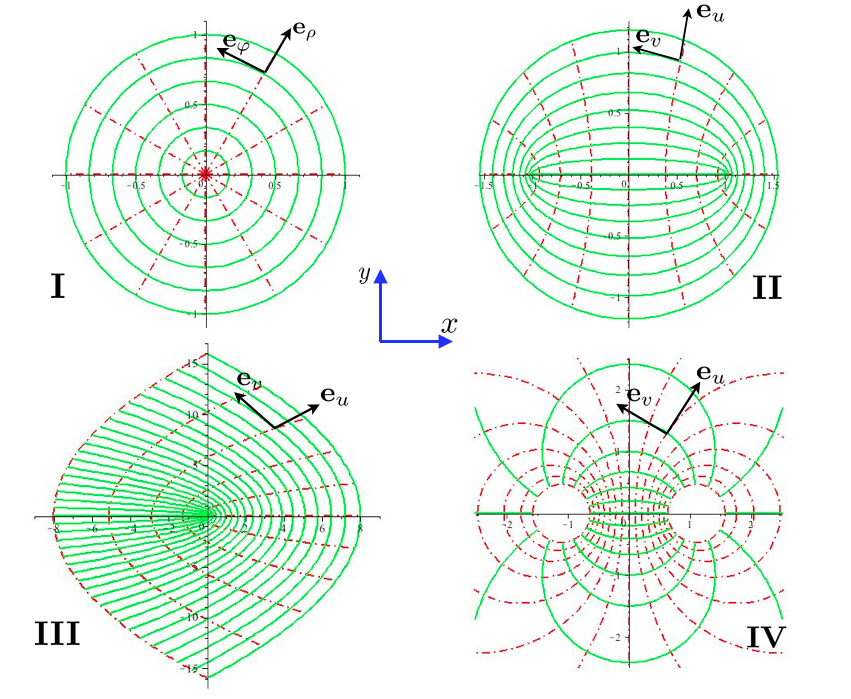
\includegraphics[width=5.0in]{VOLUMEN_1/05_Analisis_Vectorial/Figuras/Figura5_1.jpg}
\caption{Algunas coordenadas curvil�neas en 2D. Podemos apreciar algunos ejemplos de sistemas de coordenadas: en el cuadrante  I  coordenadas polares: 
$x=\rho\cos(\varphi);\quad y= \rho\ \mathrm{sen}(\varphi)$. En el cuadrante II  coordenadas  el�pticas: 
$x=a\cosh(u)\cos(v);\quad y=a\mbox{senh}(u)\mathrm{sen}(v)$. En III  coordenadas  parab�licas:  $x=\frac{1}{2}\left(u^2-v^{2}\right);\quad y=uv $ y en el cuadrante  IV  coordenadas  bipolares: 
$x^{2}+\left[y-a\cot(u)\right]^{2}=a^{2} \csc^{2}(u);\,\left[ x-a\frac{\mbox{senh}(v)}{\cosh(v)}\right] ^{2}+y^{2}=\frac{a^{2}}{\mbox{senh}^{2}(v)}$.}
\label{fig1coordcurv2d}
\end{center}
\end{figure}

\subsection{Coordenadas cartesianas}
\label{CoordenadasCartesianas}
\index{Coordenadas!cartesianas}
\index{Cartesianas!Coordenadas}
El primer caso particular lo constituyen  las coordenadas cartesianas, $(q^{1},q^{2},q^{3} )  \Longleftrightarrow (  x, y, z )$, y el vector posici�n lo construimos a partir de la ecuaci�n (\ref{VecPosicionCurvilineas}) como:
\[
\left| r\right> =x \left| \mathrm{e}_{x}\right> +y\left| \mathrm{e}_{y}\right> +z\left| \mathrm{e}_{z}\right> \Longleftrightarrow
\mathbf{r}= x\mathbf{i}+y\mathbf{j}+z\mathbf{k}\,,
\]
mientras que el vector desplazamiento diferencial tambi�n ser� inmediato a partir de (\ref{VecDesplazDiferencialCurvilineas})
\[
\mathrm{d}\mathbf{r} \\ \Rightarrow \\
\left|\mathrm{d}{r}\right>=
\left(  \frac{\partial \left| r \right>}{\partial x}\right)  \mathrm{d}x  +\left(  \frac{\partial \left| r \right>}{\partial y}\right)  \mathrm{d}y  +\left(  \frac{\partial \left| r \right>}{\partial z}\right)  \mathrm{d}z=
\mathrm{d}x\left| \mathrm{e}_{x}\right> +\mathrm{d}y\left| \mathrm{e}_{y}\right> 
+\mathrm{d}z\left| \mathrm{e}_{z}\right>\,,
\]
y, consecuentemente, los factores de escala quedan definidos como 
\[
h_{1}=h_{x}=\left\|  \frac{\partial \left| r\right> }{\partial x}\right\|  =1 \,, \quad 
h_{2}=h_{y}=\left\|  \frac{\partial \left| r\right> }{\partial y}\right\|  =1 \,, \quad 
h_{3}=h_{z}=\left\|  \frac{\partial \left| r\right> }{\partial z}\right\|  =1\,,
\]
mientras que la tr�ada ortonormal es
\[
\left| \mathrm{e}_{x}\right> =
\frac{1}{\left\|  \frac{\partial \left| r\right> }{\partial x}\right\|  }\frac{\partial \left| r\right> }{\partial x} \,, \quad 
\left| \mathrm{e}_{y}\right> =\frac{1}{\left\|  \frac{\partial \left| r\right> }{\partial y}\right\|  }\frac{\partial \left| r\right> }{\partial y} \,, \quad 
\left| \mathrm{e}_{z}\right> =\frac{1}{\left\|  \frac{\partial \left| r\right> }{\partial z}\right\|  }\frac{\partial \left| r\right> }{\partial z}\,.
\]
Finalmente, el elemento de l�nea viene definido a partir de (\ref{ElementoLineaGeneralizado}) como
\[
\left(  \mathrm{d}s\right)^{2}=
\left(  h_{1}\ \mathrm{d}x^{1}\right)^{2}+\left(  h_{2}\ \mathrm{d}x^{2}\right)^{2} +\left(  h_{3}\ \mathrm{d}x^{3}\right) ^{2} \quad \Longleftrightarrow \quad 
\mathrm{d}s^{2}=\ \mathrm{d}x^{2}+\mathrm{d}y^{2}+\mathrm{d}z^{2}\,,
\]
y el tensor m�trico ser� $g_{11}=g_{xx}=1;\quad g_{22}=g_{yy}=1;$ y $ g_{22}=g_{zz}=1\,.$


\subsection{Coordenadas cil�ndricas}
\index{Coordenadas!cil�ndricas}
El segundo caso en complejidad son las coordenadas cil�ndricas, $(q^{1},q^{2},q^{3})  \Longleftrightarrow  (\rho, \varphi, z)\,$.  Sus vectores base y su m�trica se construyen a partir de las ecuaciones (\ref{VecPosicionCurvilineas}), (\ref{VecDesplazDiferencialCurvilineas}) y  (\ref{ElementoLineaGeneralizado}) expres�ndolas como funci�n de las nuevas coordenadas. Esto es
\[
\left| r\right> =x(\rho, \varphi)  \left| \mathrm{e}_{x}\right>+y(\rho, \varphi)  \left| \mathrm{e}_{y}\right> +z\left| \mathrm{e}_{z}\right>\Longleftrightarrow
\mathbf{r}=x(\rho, \varphi)  \mathbf{i}+y(\rho, \varphi)  \mathbf{j}+z\mathbf{k}\, , 
\]
con: $\rho\geq0$, $0\leq \varphi < 2\pi$ y $-\infty<z<\infty$. 

Las componentes de $x, y, z$ del vector posici�n expresada en las nuevas coordenadas pueden ser identificadas a partir de las leyes de transformaci�n respecto a las coordenadas cartesianas:
\[
\left.
\begin{array}
[c]{l}
x=x(\rho, \varphi)  =\rho\cos(\varphi) \\
\\
y=y(\rho, \varphi)  =\rho\ \mathrm{sen}(\varphi) \\
\\
z=z
\end{array}
\right\}  \quad \Rightarrow 
\begin{array}
[c]{l}
\mathrm{d}x=\cos(\varphi)\mathrm{d}\rho-\rho\ \mathrm{sen}(\varphi)
\mathrm{d}\varphi\\
\\
\mathrm{d}y=\mathrm{sen}(\varphi)\mathrm{d}\rho+\rho\cos(\varphi)
\mathrm{d}\varphi\\
\\
\mathrm{d}z=\mathrm{d}z\,.
\end{array}
\]

Por lo que el vector posici�n en estas coordenadas es:
$
\left| r \right>=\rho\cos(\varphi)\left| \mathrm{e}_{x}\right>+
\rho \, \mathrm{sen}(\varphi) \left| \mathrm{e}_{y}\right>+
z\left| \mathrm{e}_{z}\right>\,$, donde  es f�cil identificar:

\begin{eqnarray*}
\frac{\partial }{\partial \rho} x\left(\rho,\varphi\right)&=&
\cos(\varphi) \,, \quad\quad\quad\,
\frac{\partial }{\partial \rho}y\left(\rho,\varphi\right)=
\mathrm{sen}(\varphi) \,, \quad\quad\,
\frac{\partial }{\partial \rho} z=0 \\
\frac{\partial }{\partial \varphi}x\left(\rho,\varphi\right)&=&
-\rho\ \mathrm{sen}(\varphi) \,, \quad
\frac{\partial }{\partial \varphi} y\left(\rho,\varphi\right)=
\rho \cos(\varphi)\,, \quad
\frac{\partial }{\partial \varphi} z=0 \\
\frac{\partial   }{\partial z} x(\rho, \varphi)&=&0\,, 
\qquad\qquad\quad
\frac{\partial  }{\partial z}y(\rho, \varphi)=0\,, \quad\quad\qquad
\frac{\partial }{\partial z} z=1\,,
\end{eqnarray*}
y de all� calcular los respectivos factores de escala:
\begin{align}
h_{\rho}  &  =\left\|  \frac{\partial \left| r\right>}{\partial \rho}\right\| =
\left\|  \frac{\partial \left[  x\left(\rho,\varphi\right)  \left| \mathrm{e}_{x}\right>+ y(\rho, \varphi)\left| \mathrm{e}_{y}\right>+z\left| \mathrm{e}_{z}\right>\right]  }{\partial \rho}\right\|=
\left\|  \frac{\partial x(\rho, \varphi)  }{\partial \rho}\left| \mathrm{e}_{x}\right>+\frac{\partial y(\rho, \varphi)}{\partial \rho}\left| \mathrm{e}_{y}\right>\right\| \nonumber \\
&=\left\|  \cos(\varphi) \left| \mathrm{e}_{x}\right>+
\mathrm{sen}(\varphi)\left| \mathrm{e}_{y}\right>\right\|=1 \nonumber\,.
\end{align}
Del mismo modo
\[
h_{\varphi}=\left\|  \frac{\partial \left| r\right>}{ \partial \varphi}\right\|=\rho
\,;\quad 
h_{z}=\left\|  \frac{\partial \left| r\right>}{ \partial z}\right\|  =1\,.
\]
Mientras que los vectores unitarios ser�n
\[
\begin{array}
[c]{l}
\left|  \mathrm{e}_{\rho}\right> = \frac{1}{\left\|\frac{\partial \left| r\right> }{\partial \rho}\right\|}
\frac{\partial \left| r\right> }{\partial \rho}=
\frac{\partial x(\rho, \varphi)  }{\partial \rho}
\left| \mathrm{e}_{x}\right>+\frac{\partial y(\rho, \varphi)  }
{\partial \rho}\left| \mathrm{e}_{y}\right>=
\cos(\varphi) \left| \mathrm{e}_{x}\right>+\mathrm{sen}(\varphi) \left| \mathrm{e}_{y}\right>\,,\\
\\
\left|  \mathrm{e}_{\varphi}\right> =\frac{1}{\left\| \frac{\partial \left| r\right> }{\partial \varphi}\right\|
}\frac{\partial \left| r\right> }{\partial \varphi}=\frac{1}{\rho}\left(  \frac{\partial x(\rho, \varphi)  }
{\partial \varphi} \left| \mathrm{e}_{x}\right>
+\frac{\partial y\left( \rho,\varphi\right)  }{\partial \varphi} \left| \mathrm{e}_{y}\right>\right)=
-\mathrm{sen}(\varphi) \left| \mathrm{e}_{x}\right>+\cos(\varphi) \left| \mathrm{e}_{y}\right>\,, \\
\\
\left|  \mathrm{e}_{z}\right> =\frac{1}{\left\|  \frac{\partial \left| r\right> }
{\partial z}\right\|  }\frac{\partial \left| r\right> }{\partial z}=
\frac{\partial  z }{\partial z}\left| \mathrm{e}_{z}\right>=\left| \mathrm{e}_{z}\right>\,.
\end{array}
\]
Claramente, el sistema de coordenadas, para el caso 2D ($z= 0$) se reduce al sistema de coordenadas polares que ilustramos en el cuadrante I de la figura \ref{fig1coordcurv2d}.  


El caso 3D lo ilustramos en la figura \ref{3DCilindricasEsfericas}, izquierda y puede apreciarse que el vector unitario $\left|  \mathrm{e}_{\rho}\right>$ es un vector normal a las superficies cil�ndricas y apunta en la direcci�n donde crece el radio $\rho$. El vector unitario $\left|  \mathrm{e}_{\varphi}\right>$ es tangente a las superficies cil�ndricas, perpendicular a los planos $\varphi= constante$ y apunta en la direcci�n donde aumenta el �ngulo azimutal $\varphi$. El vector $\left|  \mathrm{e}_{z}\right>$ es el mismo vector cartesiano $\left|  {\mathrm{k}} \right>$.


La expresi�n para el vector desplazamiento infinitesimal ser�
\[
\mathrm{d}\left| r \right>= 
  \frac{\partial \left| r \right> }{\partial \rho}  \mathrm{d}\rho +
  \frac{\partial \left| r \right>}{\partial \varphi}  \mathrm{d}\varphi+
  \frac{\partial \left| r \right>}{\partial z}\mathrm{d} z =  
  \mathrm{d}\rho\left|  \mathrm{e}_{\rho}\right> +  \rho \mathrm{d}\varphi \left|  \mathrm{e}_{\varphi}\right> + \mathrm{d} z\left|  \mathrm{e}_{z}\right> \,.
\]

Notemos que en este caso, y a diferencia de las coordenadas cartesianas,  si $\varphi$ var�a en una cantidad $\mathrm{d}\varphi$, con $\rho$ y $z$ constantes, entonces el desplazamiento no ser� $\mathrm{d}\varphi$ sino $\rho \mathrm{d}\varphi$.

El elemento de l�nea viene definido como
\[
\mathrm{d}s^{2}=
\left(  h_{1} \mathrm{d}q^{1}\right)^{2}+\left(  h_{2} \mathrm{d}q^{2}\right)^{2}+\left(  h_{3} \mathrm{d}q^{3}\right)^{2}  \quad \Longleftrightarrow\quad \mathrm{d}s^{2}=
\mathrm{d}\rho^{2}+\rho^{2}\ \mathrm{d}\varphi^{2}+\mathrm{d}z^{2}\,,
\]
y el tensor m�trico:
\[
g_{11}=g_{\rho\rho}=1;\quad g_{22}=g_{\varphi\varphi}=\rho^{2};\quad g_{33}=g_{zz}=1\,.
\]


\subsection{Coordenadas esf�ricas}
\index{Coordenadas!esfericas}
\index{Factores de escala!coordenadas esf�ricas}
Para construir el sistema de coordenadas esf�ricas tenemos:
\[
(q^{1},q^{2},q^{3})  \Longleftrightarrow 
\left(r,\theta,\varphi\right) \,,
\]
\[
\left| r\right> =x\left(r,\theta,\varphi\right)   \left|
\mathrm{i}\right> +y\left(r,\theta,\varphi\right)   \left|
\mathrm{j}\right> +z\left(r,\theta,\varphi\right)   \left|
\mathrm{k}\right>  \Longleftrightarrow \mathbf{r}=
x\left(r,\theta,\varphi\right)   
\mathbf{i}+y\left(r,\theta,\varphi\right)   
\mathbf{j}+z\left(r,\theta,\varphi\right) \mathbf{k}\,.
\]
Con: $r\geq0$,  $0\leq\theta \leq \pi$ y $0\leq\varphi< 2\pi$. A $r$ se le denomina la coordenada radial, a $\theta$ la coordenada polar y a $\varphi$ la coordenada azimutal. 

Tendremos entonces:
\[
\mathrm{d}\mathbf{r} \\ \Rightarrow \\ \left| \mathrm{d}{r}\right>=
\frac{\partial \left| r \right>}{\partial r}  \mathrm{d}r+
\frac{\partial \left| r \right>}{\partial \theta}  \mathrm{d}\theta+
\frac{\partial \left| r \right>}{\partial \varphi}  \mathrm{d}\varphi \,.
\]

Estas cantidades pueden ser identificadas de las leyes de transformaci�n respecto a las coordenadas cartesianas
\[
\left.
\begin{array}
[c]{l}
x=x\left(r,\theta,\varphi\right) =r\cos(\varphi)\mathrm{sen}(\theta)\\
\\
y=y\left(r,\theta,\varphi\right)  =r\ \mathrm{sen}(\varphi)
\mathrm{sen}(\theta)\\
\\
z=z\left(r,\theta,\varphi\right)  =r\cos(\theta)
\end{array}
\right\}  \quad \Rightarrow 
\begin{array}
[c]{l}
\mathrm{d}x=\cos(\varphi) \mathrm{sen}(\theta)\mathrm{d}r-r \ \mathrm{sen}(\varphi)\mathrm{sen}(\theta)\mathrm{d}\varphi
+r\cos(\varphi)\cos(\theta)\mathrm{d}\theta\\
\\
\mathrm{d}y=\mathrm{sen}(\varphi)\mathrm{sen}(\theta)\mathrm{d} r+
r \cos(\varphi)\mathrm{sen}(\theta)\mathrm{d}\varphi+r �
\mathrm{sen} (\varphi)\cos(\theta)\mathrm{d}\theta\\
\\
\mathrm{d}z=\cos(\theta)\mathrm{d}r-r \ \mathrm{sen}(\theta)\mathrm{d}\theta
\end{array}
\]

El vector posici�n es de la forma
\[
\left| r \right> = 
r \ \mathrm{sen}(\theta)\cos(\varphi)\left| \mathrm{e}_{x}\right>+
r \ \mathrm{sen}(\theta)\mathrm{sen}(\varphi)\left| \mathrm{e}_{y}\right> +
r \cos(\theta) \left| \mathrm{e}_{z}\right>\,.
\]

Derivando:
\begin{eqnarray}
\label{derivaesfericas}
\frac{\partial x\left(r,\theta,\varphi\right)}{\partial r}&=&
\cos(\varphi)\mathrm{sen}(\theta) \,, \quad\, \quad \quad
\frac{\partial y\left(r,\theta,\varphi\right)  }{\partial r}
=\mathrm{sen}(\varphi)\mathrm{sen}(\theta) \,,\quad\, \quad
\frac{\partial z\left(r,\theta,\varphi\right)}{\partial r}=\cos(\theta)
\nonumber \\
\frac{\partial x\left(r,\theta,\varphi\right)}{\partial \theta}&=&
r\cos(\varphi)\cos(\theta) \,, \quad \quad 
\frac{\partial y\left(r,\theta,\varphi\right)  }{\partial \theta}=
r \ \mathrm{sen}(\varphi)\cos(\theta) \,, \quad
\frac{\partial z\left(r,\theta,\varphi\right)  }{\partial \theta}=
-r \ \mathrm{sen}(\theta)\\
\frac{\partial x\left(r,\theta,\varphi\right)}{\partial \varphi}&=&
-r \ \mathrm{sen}(\varphi)\mathrm{sen}(\theta) \,, \quad
\frac{\partial y\left(r,\theta,\varphi\right)  }{\partial \varphi}
=r\cos(\varphi)\mathrm{sen}(\theta) \,, \quad
\frac{\partial z\left(r,\theta,\varphi\right)  }{\partial \varphi}=0\nonumber \,.
\end{eqnarray}

Los factores de escala son los siguientes:
\begin{eqnarray}
h_{r}  &=&\left\|  \frac{\partial\left| r\right> }{\partial r}\right\|  =
\left\|\cos(\varphi)\mathrm{sen}(\theta)\left| \mathrm{e}_{x}\right>+
\mathrm{sen}(\varphi)\mathrm{sen}(\theta) \left| \mathrm{e}_{y}\right>+
\cos(\theta)\left| \mathrm{e}_{z}\right>\right\| \nonumber \\
&=& \sqrt{\cos^{2}(\varphi) \mathrm{sen}^{2}(\theta)+\mathrm{sen}^{2}(\varphi)\mathrm{sen}^{2}(\theta)+\cos^{2}(\theta)}=1\,, 
\\ \nonumber \\
h_{\theta}  &=&\left\|  \frac{\partial\left| r \right> }{\partial \theta}\right\|  =\left\|  r\cos(\varphi)\cos(\theta) \left| \mathrm{e}_{x}\right>+
r\mathrm{sen}(\varphi)\cos(\theta) \left| \mathrm{e}_{y}\right>-
r\mathrm{sen}(\theta) \left| \mathrm{e}_{z}\right>\right\| \nonumber \\
&=& \sqrt{\left(  r\cos(\varphi)\cos(\theta)\right)^{2}+\left(
r\mathrm{sen}(\varphi)\cos(\theta)\right)^{2}+
\left(  r\mathrm{sen}(\theta)\right)^{2}}= r \,, \\  \nonumber \\
h_{\varphi}&=&
\left\|\frac{\partial\left| r \right>}{\partial \varphi}\right\|  = 
\left\|-r\mathrm{sen}(\varphi)\mathrm{sen}(\theta)\left| \mathrm{e}_{x}\right>+
r\cos(\varphi)\mathrm{sen}(\theta) \left| \mathrm{e}_{y}\right>\right\| \nonumber \\
&=&\sqrt{\left(r\mathrm{sen}(\varphi)\mathrm{sen}(\theta)\right)^{2}+
\left(  r\cos(\varphi)\mathrm{sen}(\theta)\right)^{2}} =  
r \ \mathrm{sen}(\theta)\,.
\end{eqnarray}

Mientras que para los vectores unitarios tenemos
\[
\begin{array}
[c]{l}
\left|  \mathrm{e}_{r}\right> =
\frac{1}{h_r}\frac{\partial \left| r \right> }{\partial r}=
\cos(\varphi)\mathrm{sen}(\theta)\left| \mathrm{e}_{x}\right>+
\mathrm{sen}(\varphi)\mathrm{sen}(\theta) \left| \mathrm{e}_{y}\right>+
\cos(\theta)\left| \mathrm{e}_{z}\right>\,, \\ \\
\left| \mathrm{e}_{\theta}\right> =
\frac{1}{h_{\theta}}\frac{\partial \left| {r}\right> }{\partial \theta}=
\cos(\varphi)\cos(\theta) \left| \mathrm{e}_{x}\right>+
\mathrm{sen}(\varphi)\cos(\theta) \left| \mathrm{e}_{y}\right>-
\mathrm{sen}(\theta) \left| \mathrm{e}_{z}\right>\,,
\\ \\
\left|  \mathrm{e}_{\varphi}\right> =
\frac{1}{h_{\varphi}}\frac{\partial \left| r\right> }{\partial \varphi}=
-\mathrm{sen}(\varphi) \left| \mathrm{e}_{x}\right>+\cos(\varphi) \left| \mathrm{e}_{y}\right> \,.
\end{array}
\]

El desplazamiento infinitesimal en estas coordenadas es de la forma
\[
\mathrm{d}\left| r \right>= 
\left(  \frac{\partial \left| r \right> }{\partial r}\right)  \mathrm{d}r+
\left(\frac{\partial \left| r \right>}{\partial \theta}\right)  
\mathrm{d}\theta+\left(  \frac{\partial \left| r \right>}{\partial\varphi}\right)
\mathrm{d} \varphi =  
\mathrm{d}r\left|  \mathrm{e}_{r}\right> +  
r \mathrm{d}\theta \left| \mathrm{e}_{\theta}\right> + 
r \ \mathrm{sen}(\theta) 
\mathrm{d} \varphi \left| \mathrm{e}_{\varphi}\right> \,.
\]

Por lo tanto, para el elemento de l�nea tenemos
\[
\left(  \mathrm{d}s\right)^{2}=\left(  h_{1}\ \mathrm{d}q^{1}\right)
^{2}+\left(  h_{2}\ \mathrm{d}q^{2}\right)^{2}+\left(  h_{3}\ \mathrm{d}
q^{3}\right)^{2}\quad\Longleftrightarrow\quad\mathrm{d}s^{2}=
\mathrm{d}r^{2}+r^{2}\mathrm{d}\theta^{2}+ r^{2}\mathrm{sen}^{2}(\theta) \mathrm{d}\varphi^{2} \,.
\]
Y para el tensor m�trico
\[
g_{11}=g_{rr}=1;\quad g_{22}=g_{\theta\theta }=r^{2} ;\quad
g_{33}=g_{\varphi\varphi}=r^{2}\mathrm{sen}^{2}(\theta)\,.
\]

\begin{figure}[ptb]
\begin{center}
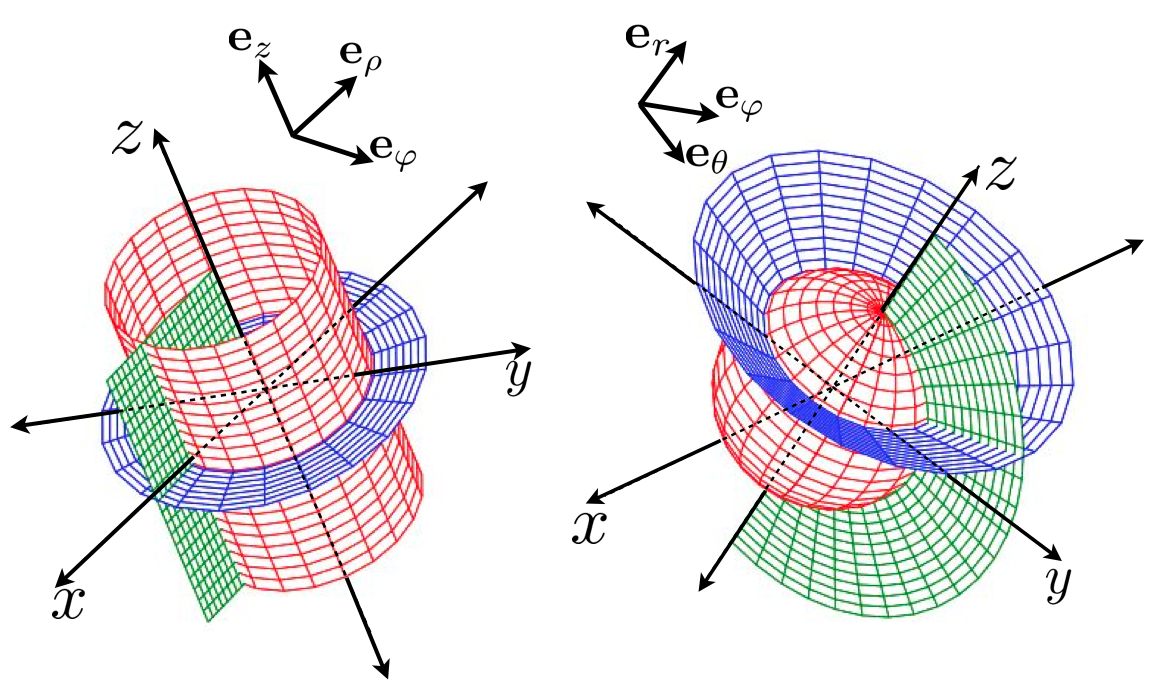
\includegraphics[width=4.5in]{VOLUMEN_1/05_Analisis_Vectorial/Figuras/Figura5_2.jpg}
\end{center}
\caption{Coordenadas cil�ndricas y esf�ricas. Para el caso de las coordenadas cil�ndricas (figura izquierda), el vector unitario $\left|  \mathrm{e}_{\rho}\right>$ es un vector normal a las superficies cil�ndricas y apunta en la direcci�n donde crece el radio $\rho$. El vector unitario $\left|  \mathrm{e}_{\varphi}\right>$ es tangente a las superficies cil�ndricas, perpendicular a los planos $\varphi= constante$ y apunta en la direcci�n donde aumenta el �ngulo azimutal $\varphi$. El vector $\left|  \mathrm{e}_{z}\right>$ es el mismo vector cartesiano $\left|  {\mathrm{k}} \right>$.}
\label{3DCilindricasEsfericas}
\end{figure}

\subsection{Otros sistemas coordenados}
Por completitud, enumeraremos algunos otros sistemas de coordenadas y dejaremos al lector la labor de calcular los vectores unitarios y la m�trica del espacio expresada en esas coordenadas.

\begin{itemize}
\item {\bf{Coordenadas toroidales}}
\label{CoordenadasToroidales}
\index{Coordenadas!toroidales}
\index{Toroidales!coordenadas}
\[
\left( q^{1},q^{2},q^{3}\right)  \Longleftrightarrow \left(\sigma,\tau,\phi\right) 
\]
\[
\left| {r}\right> =
x\left(\sigma,\tau,\phi\right)  \left| \mathrm{e}_{x}\right>+
y\left(\sigma,\tau,\phi\right)  \left| \mathrm{e}_{y}\right> +
z\left(\sigma,\tau,\phi\right)  \left| \mathrm{e}_{z}\right>\Longleftrightarrow 
\mathbf{r}=
x\left(\sigma,\tau,\phi\right)   \mathbf{i}+
y\left(\sigma,\tau,\phi\right)   \mathbf{j}+
z\left(\sigma,\tau,\phi\right)   \mathbf{k} \,.
\]
Con $0\leq\sigma<2\pi$, $0\leq\tau<\infty$ y $0\leq\phi<2\pi$.

La transformaci�n de coordenadas est� definida de la siguiente forma (con $a$ constante)
\[
x = a \ \frac{\mbox{senh}(\tau)}{\cosh (\tau) - \cos (\sigma)} \cos(\phi) \,, \quad
y = a \ \frac{\mbox{senh}(\tau)}{\cosh (\tau) - \cos (\sigma)} \mathrm{sen} (\phi)  \,, \quad
z = a \ \frac{\mathrm{sen}(\sigma)}{\cosh (\tau) - \cos (\sigma)}\,,
\]
Las superficies $\tau$ constante representan toros alrededor del eje $z$; las superficies $\sigma$ constante son esferas con centro sobre el eje $z$ y finalmente las superficies $\phi$ constante son planos que contiene al eje $z$.

La m�trica en estas coordenadas es:
\begin{eqnarray*}
\mathrm{d}s^{2}&=&\left(  h_{1}\ \mathrm{d}q^{1}\right)
^{2}+\left(  h_{2} \ \mathrm{d}q^{2}\right)^{2}+\left(  h_{3}\ \mathrm{d}q^{3}\right)^{2} \,, \\
&=& 
\left(  \frac{a}{\cosh (\tau) - \cos (\sigma)}  \right)^2 \mathrm{d} \sigma^{2}+
\left(  \frac{a}{\cosh (\tau) - \cos (\sigma)}  \right)^2 \mathrm{d}\tau^{2}+ 
\left(  \frac{a\ \mbox{senh}(\tau) }{\cosh (\tau) - \cos (\sigma)}  \right)^2 \mathrm{d}\phi^{2}\,.
\end{eqnarray*}


\item {\bf{Coordenadas elipsoidales}}
\index{Coordenadas!elipsoidales}
\index{Elipsoidales!coordenadas}
Dados tres n�meros $a,b$ y $c$, con $a>b>c>0$, la ecuaci�n
\[
\frac{x^{2}}{a^{2}+\alpha}+\frac{y^{2}}{b^{2}+\alpha}+\frac{z^{2}}
{c^{2}+\alpha}=1 \,,
\]
representa las superficies cu�dricas\footnote{N�tese que la
proyecci�n de estas superficies en el plano $xy$
representan curvas c�nicas homofocales.} homofocales (es decir, con el mismo foco u origen en $\left(x=0,y=0,z=0\right))$. 

Dependiendo del valor del par�metro $\alpha$, estas ecuaciones representar�n superficies
\[
\begin{array}
[c]{ccc}
\text{Elipsoides} & \text{si} & \alpha>-c^{2}\\
\text{Hiperboloides de una hoja} & \text{si} & -c^{2}>\alpha>-b^{2}\\
\text{Hiperboloides de dos hojas} & \text{si} & -b^{2}>\alpha>-c^{2}
\end{array}
\]

Esto quiere decir que por cada punto $(x,y,z)  $\ del espacio, pasan tres superficies cu�dricas (dependiendo del valor de $\alpha$).
Conocidos $a,b$ y $c$ y el punto, $\left(  x=x_{0},y=y_{0},z=z_{0}\right)$,  
los valores de $\alpha$ vienen dados por las ra�ces de la ecuaci�n
c�bica
\[
\frac{x^{2}}{a^{2}+\alpha}+\frac{y^{2}}{b^{2}+\alpha}+\frac{z^{2}}
{c^{2}+\alpha}=1\quad \Rightarrow  \alpha^{3}+\Delta\ \alpha^{2}
+\Phi\ \alpha+\Omega=0\,,
\]
con
\begin{align*}
\Delta &  =x_{0}^{2}+y_{0}^{2}+z_{0}^{2}-a^{2}-b^{2}-c^{2} \,,\\
& \\
\Phi &  =\left(  b^{2}+c^{2}\right)  x_{0}^{2}+\left(  a^{2}+c^{2}\right)
y_{0}^{2}+\left(  a^{2}+b^{2}\right)  z_{0}^{2}-a^{2}b^{2}-\left(  a^{2}
+b^{2}\right)  c^{2} \,,\\
& \\
\Omega &  =x_{0}^{2}b^{2}c^{2}+y_{0}^{2}a^{2}c^{2}+z_{0}^{2}a^{2}b^{2}-a^{2}b^{2}c^{2}\,.
\end{align*}

Las ra�ces de esta ecuaci�n $\left(\alpha_{1}=\lambda;\alpha_{2} = \mu;\alpha_{3}=\nu\right)$ definen las coordenadas elipsoidales del punto $(x,y,z)  =\left(  x\left(  \lambda,\mu,\nu\right)  ,y\left(\lambda,\mu,\nu\right)  ,z\left(  \lambda,\mu,\nu\right)  \right)$.

Tenemos entonces:
\[
\left( q^{1},q^{2},q^{3}\right)  \Longleftrightarrow  \left(\lambda,\mu,\nu\right) \,,
\]
\[
\left| {r}\right> =x\left(\lambda,\mu,\nu\right) \left| \mathrm{e}_{x}\right>+
y\left(\lambda,\mu,\nu\right)  \left| \mathrm{e}_{y}\right> +
z\left(\lambda,\mu,\nu\right)  \left| \mathrm{e}_{z}\right> \Longleftrightarrow 
\mathbf{r}=
x\left(\lambda,\mu,\nu\right)   \mathbf{i}+
y\left(\lambda,\mu,\nu\right)   \mathbf{j}+
z\left(\lambda,\mu,\nu\right)  \mathbf{k} \,.
\]
Y la ley de transformaci�n:
\[
x  =\sqrt{\frac{\left(  a^{2}+\lambda\right)  \left(  a^{2}+\mu\right)  \left(  a^{2}+\nu\right)  }{\left(
a^{2}-b^{2}\right)  \left(  a^{2}-c^{2}\right)  }}\,, \quad
y  = \sqrt{\frac{\left(  b^{2}
+\lambda\right)  \left(  b^{2}+\mu\right)  \left(  b^{2}+\nu\right)  }{\left(
b^{2}-a^{2}\right)  \left(  b^{2}-c^{2}\right)  }} \,, \quad
z  =\sqrt{\frac{\left(  c^{2}
+\lambda\right)  \left(  c^{2}+\mu\right)  \left(  c^{2}+\nu\right)  }{\left(
c^{2}-b^{2}\right)  \left(  c^{2}-a^{2}\right)  }}\,,
\]
por cual la m�trica ser�
\[
\mathrm{d}s^{2} =\frac{\left(  \lambda-\mu\right)  \left(  \lambda-\nu\right)  }{4\left(  a^{2}+\lambda\right)  \left(  b^{2}+\lambda\right) \left(  c^{2}+\lambda\right)  }\mathrm{d}\lambda^{2}+\frac{\left(  \mu
-\lambda\right)  \left(\mu-\nu\right)  }{4\left(  a^{2}+\mu\right)  \left(b^{2}+\mu\right)  \left(  c^{2}+\mu\right)  }\mathrm{d}\mu^{2}+ \frac{\left(  \nu-\mu\right)  \left(  \nu-\lambda\right)  }{4\left(  a^{2}+\nu\right)  \left(  b^{2}+\nu\right)  \left( c^{2}+\nu\right)  }\mathrm{d}\nu^{2}\,.
\]

\end{itemize}

\subsection{Curvas y par�metros}
\label{CurvasParametros}
\index{Curvas parametrizadas}
Tal y como se expuso en la secci�n \ref{ComienzoDerivacionVectores}, los vectores podr�n ser constantes o variables y, esa caracter�stica se verificar� tanto en las componentes como en la base. En esta secci�n lo mostramos para el caso de los vectores 3D, pero el concepto es generalizable a cualquier dimensi�n. Esto quiere decir que, cuando un vector es variable podr�n variar su m�dulo, su direcci�n, su sentido, todo junto o por separado. Obviamente, esta variabilidad del vector depender� de la base en la cual se exprese, por lo cual un mismo vector podr� tener una componente constante en una base y variable en otra, es decir
\begin{equation}
\label{VectorVariable}
\left|a \right>_{(t)}=a^{k}(t)  \left|{e}_{k}\right>_{(t)}=\tilde{a}^{k}\left| {\tilde{e}}_{k}\right>_{(t)}=\hat{a}^{k}(t) \left| {\hat{e}}_{k}\right>\,.
\end{equation}

De esta manera, cuando uno considera un vector variable,  
$\left|a\right>_{(t)} \Longleftrightarrow 
\mathbf{a}(t)$, podemos establecer un cociente incremental:
\[
\lim_{\Delta t\rightarrow0}\frac{\left|  a\right>_{\left(t+\Delta t\right)  }-\left|  a\right>_{(t)  }}{\Delta t}  
=
\lim_{\Delta t\rightarrow0}\frac{\Delta\left|  a\right>_{(t)}}{\Delta t}=\frac{\mathrm{d}  \left|  a\right>_{(  t)  }  }{\mathrm{d}t}.
\]
La misma propuesta se cumplir� para las formas diferenciales $_{(t)}\left<a\right|$. 

Como siempre, las propiedades de esta diferenciaci�n ser�n:
\begin{eqnarray*}
\frac{\mathrm{d}}{\mathrm{d}t} \left(  \left|  a\right> _{(t)  }+\left| b\right> _{(t)  }\right)   & = &
\frac{\mathrm{d}  \left|  a\right> _{(t)}}{\mathrm{d}t}+\frac{\mathrm{d}  \left|  b\right> _{(t)  }  }{\mathrm{d}t} \ ,
\\
\frac{\mathrm{d}} {\mathrm{d}t} \left(  \alpha(t)  \left|  a\right>_{(t)  }\right) &= &\frac{\mathrm{d} \alpha(t)}{\mathrm{d}t}\left|  a\right>_{(t)  } +\alpha(t)  \frac{\mathrm{d} \left| a\right> _{(t)  }} {\mathrm{d}t}
 \quad \text{y} \\
\frac{\mathrm{d}}{\mathrm{d}t}\left(  _{(t)  }\left< a\right.  \left| b\right> _{(t)  }\right)  & = & \frac{\mathrm{d}  (_{(t)}\left< a\right| ) }{\mathrm{d}t} 
\left|  b\right>_{(t)} + _{(t)}\left< a\right| \frac{\mathrm{d}\left|  b\right> _{(t)}}{\mathrm{d}t}\,.
\end{eqnarray*}
Entonces reproducimos aqu� la ecuaci�n (\ref{dAdtvariable}), de la secci�n \ref{DerivacionVectores3D}, ahora en notaci�n de Dirac:
\begin{equation}
\label{DerivaVector}
\left|  a\right> _{(t)  }=a^{k}(t)  \left| {e}_{k}\right> _{(t)  }\quad \Rightarrow 
\frac{\mathrm{d}  \left|  a\right> _{(t)}}{\mathrm{d}t}=\frac{\mathrm{d} }{\mathrm{d}t}\left(  a^{k}(t)  \left| {e}_{k}\right> _{(t)  }\right)  =
\frac{\mathrm{d }a^{k}(t)  }{\mathrm{d}t}\left|  {e}_{k}\right> _{(t)  }+a^{k}(t)  \frac{\mathrm{d}  \left|  {e}_{k}\right> _{(t)}  }{\mathrm{d}t}\,,
\end{equation}
con lo cual, como dijimos en \ref{DerivacionVectores3D}, hay que tener cuidado al derivar vectores y cerciorarse de la dependencia funcional de la base y componentes. Habr� sistemas de coordenadas (bases de vectores) que ser�n constantes y otros con bases variables. 


Podemos generalizar la ecuaci�n (\ref{DerivaVector}) si consideramos una curva descrita por un radio vector $ \left| r \right>$ funci�n de un par�metro $\lambda$, de manera que el vector posici�n, \textbf{en coordenadas cartesianas},  queda escrito como 
$
 \left| r \right>= \mathbf{r}(\lambda) = \mathbf{r}\left( x(\lambda), y(\lambda), z(\lambda)  \right) 
$, 
donde las funciones:  $\{x(\lambda), y(\lambda), z(\lambda)\}$ son las ecuaciones param�tricas de la curva descrita por el vector posici�n $\mathbf{r}$. 

Para el  vector desplazamiento infinitesimal $\left|{\mathrm{d}r}\right>=
(\mathrm{d}x(\lambda),\mathrm{d}y(\lambda),\mathrm{d}z(\lambda)) $, a lo largo de la curva descrita por el par�metro $\lambda$, resulta:
 \[
 \left|{\mathrm{d}r}\right> =
 \mathrm{d}\mathbf{r}\left(x(\lambda), y(\lambda), z(\lambda)  \right)    =
\frac{ \mathrm{d} \left( \mathbf{r}(\lambda) \right) }{\mathrm{d} \lambda}\mathrm{d}\lambda=
\left[ \frac{\mathrm{d} x}{\mathrm{d}\lambda} \frac{\partial\mathbf{r}}{\partial x} +\frac{\mathrm{d} y }{\mathrm{d}\lambda}\frac{\partial\mathbf{r}}{\partial y  }+\frac{\mathrm{d} z}{\mathrm{d}\lambda}\frac{\partial\mathbf{r}}{\partial z}\right]  \mathrm{d}\lambda\,,
 \]
con lo cual podemos hacer la siguiente asociaci�n:
\[
\frac{\mathrm{d}\left(  \ \right)  }{\mathrm{d}\lambda} \quad \Leftrightarrow \quad
\frac{\mathrm{d} x}{\mathrm{d}\lambda}\frac{\partial\left( \ \right)  }{\partial x}+\frac{\mathrm{d} y  }{\mathrm{d}\lambda}\frac{\partial\left( \ \right)  }{\partial y  }+\frac{\mathrm{d} z }{\mathrm{d}\lambda}\frac{\partial\left( \ \right)  }{\partial z  } \,,
\]
y considerar a las cantidades $\left(\frac{\mathrm{d} x}{\mathrm{d}\lambda},\frac{\mathrm{d} y  }{\mathrm{d}\lambda},\frac{\mathrm{d} z }{\mathrm{d}\lambda}\right)$ como las componentes del vector $\mathrm{d}
\mathbf{r}(\lambda) $  (y, en general, del operador 
$\frac{\mathrm{d}\left( \ \right)  }{\mathrm{d}\lambda}$) tangente a la trayectoria parametrizada con $\lambda$.
M�s a�n, podemos asociar a las cantidades: $\left(  \frac{\partial\left( \ \right)}{\partial x},\frac{\partial\left( \ \right)  }{\partial y },
\frac{\partial\left(\ \right)  }{\partial z }\right) $ con los vectores base en esas coordenadas.
Este tipo de parametrizaci�n es la que hemos usado en los cursos de mec�nica, all� el par�metro utilizado ha sido el tiempo. 

Otra forma alternativa de parametrizar el vector posici�n es a trav�s de funciones que representen la curva espacial: 
\[
 \left| r \right>= \mathbf{r}(\lambda) = \mathbf{r}\left(\lambda, f ( \lambda ), g(  \lambda)  \right) \,,
\]
o por medio de la intersecci�n de superficies $F(x,y,z)=0$ y $G(x,y,z)=0$.


\begin{figure}[h]
\begin{center} 
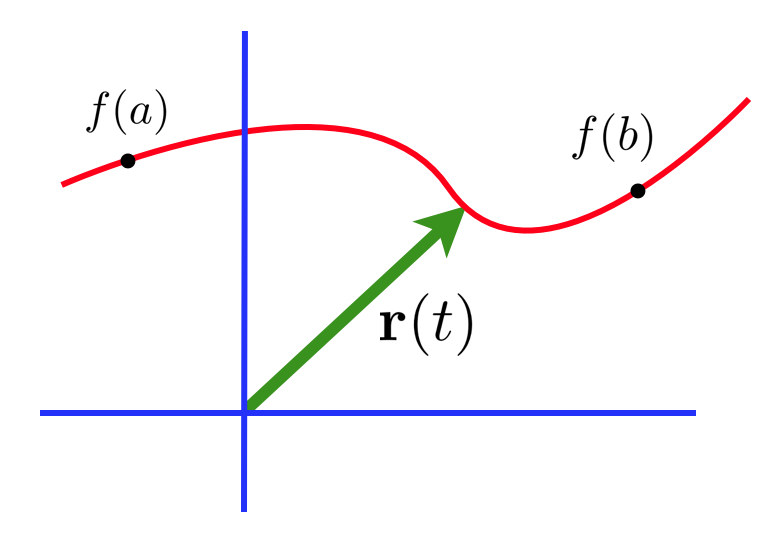
\includegraphics[width=3.0in]{VOLUMEN_1/05_Analisis_Vectorial/Figuras/Figura5_3}
\caption{Vector posici�n ${\bf r}(t)$, en $\mathds{R}^{2}$, que describe param�tricamente una curva.}
\label{FigVectorR2}
\end{center}
\end{figure}
%%%%%%%%%%%%%%%%%

Por otro lado, el cuadrado de la distancia infinitesimal recorrida es:
\[
(\mathrm{d}s)^2=\mathrm{d}\mathbf{r}(\lambda) \cdot  \mathrm{d}\mathbf{r}(\lambda)= \frac{ \mathrm{d} \left(\mathbf{r}(\lambda) \right) }{\mathrm{d} \lambda} \cdot \frac{ \mathrm{d} \left(\mathbf{r}(\lambda) \right)}{\mathrm{d} \lambda} (\mathrm{d}\lambda )^{2}=
(\mathrm{d}x({\lambda}))^2+(\mathrm{d}y({\lambda}))^2+(\mathrm{d}z({\lambda}))^2\,,
\] 
entonces
\[
\left(\frac{\mathrm{d}s}{\mathrm{d}\lambda}\right)^2= \frac{ \mathrm{d} \left( \mathbf{r}(\lambda) \right) }{\mathrm{d} \lambda} \cdot \frac{ \mathrm{d} \left(\mathbf{r}(\lambda) \right)}{\mathrm{d} \lambda}\,,
\]
por lo tanto, la longitud de arco entre dos puntos sobre la curva $ \mathbf{r}(\lambda)$ ser�
\[
s=\int_{\lambda_1}^{\lambda_2} \left[ \frac{ \mathrm{d} \left( \mathbf{r}(\lambda) \right) }{\mathrm{d} \lambda} \cdot \frac{ \mathrm{d} \left(\mathbf{r}(\lambda) \right)}{\mathrm{d} \lambda} \right]^{1/2}\mathrm{d} \lambda\,.
\]

Consideramos ahora  un conjunto de coordenadas generalizadas:\index{Coordenadas generalizadas}
$\left(  q^{1}(\lambda)  ,q^{2}(\lambda)  ,q^{3}(\lambda)
\right)$, tendremos 
\[
\left| {r}\right> =\mathbf{r}(\lambda) =\mathbf{r}\left(
q^{1}(\lambda)  ,q^{2}(\lambda)  ,q^{3}\left(
\lambda\right)  \right) \,,
\]
por lo tanto
\[
\mathrm{d}\mathbf{r}\left(  q^{i}(\lambda) \right) =
\frac{\mathrm{d} q^{1}}{\mathrm{d}\lambda}\mathrm{d}\lambda
\frac{\partial\mathbf{r}}{\partial q^{1}  } +
\frac{\mathrm{d} q^{2} }{\mathrm{d}\lambda}\mathrm{d}\lambda\frac{\partial\mathbf{r}}{\partial q^{2}} +
\frac{\mathrm{d} q^{3}}{\mathrm{d}\lambda}\mathrm{d}\lambda
\frac{\partial\mathbf{r}}{\partial q^{3}} \quad \Rightarrow  
\frac{\mathrm{d}\mathbf{\mathbf{r}}}{\mathrm{d}\lambda}    =
\frac{\mathrm{d} q^{1}}{\mathrm{d}\lambda}
\underset{\mathbf{u}_1 }{\underbrace{\frac{\partial\mathbf{r}}
{\partial q^{1}  }}} +
\frac{\mathrm{d} q^{2}}{\mathrm{d}\lambda}
\underset{\mathbf{u}_2 }{\underbrace{\frac{\partial\mathbf{r}}
{\partial q^{2} }}} +
\frac{\mathrm{d} q^{3}}{\mathrm{d}\lambda}
\underset{\mathbf{u}_3 }{\underbrace{\frac{\partial\mathbf{r}}
{\partial q^{3}  }}}\,,
\]
donde: $\left\{  \mathbf{u}_1 =\frac{\partial\mathbf{r}}{\partial
q^{1}  }, \mathbf{u}_2 =\frac{\partial
\mathbf{r}}{\partial q^{2} },\mathbf{u}_3
=\frac{\partial\mathbf{r}}{\partial q^{3}  }\right\}$,   son la base del vector $\frac{\mathrm{d}\mathbf{r}(\lambda)  }{\mathrm{d}\lambda}$ tangente a la curva descrita por $\mathbf{r}(\lambda)$.

Como sabemos, el m�dulo del vector $\left\|  \mathrm{d}\mathbf{r}(\lambda)  \right\|  $ representar� la longitud de arco $\mathrm{d}s$ para esa curva. Por consiguiente
\begin{align*}
(\mathrm{d}s)^{2}   =\mathrm{d}\mathbf{r}(\lambda) \cdot  \mathrm{d}\mathbf{r}(\lambda) & =  
\frac{ \mathrm{d} \left( \mathbf{r}(\lambda) \right) }{\mathrm{d} \lambda} \cdot \frac{ \mathrm{d} \left(\mathbf{r}(\lambda) \right)}{\mathrm{d} \lambda} (\mathrm{d}\lambda )^{2} =  
\frac{\mathrm{d} q^{i}}{\mathrm{d} \lambda} \frac{\partial \left(\mathbf{r}(\lambda) \right) }{\partial q^{i}} \cdot  
\frac{\mathrm{d} q^{j}}{\mathrm{d}\lambda} \frac{\partial\left(\mathbf{r}(\lambda)\right)}
{\partial q^{j}}  (\mathrm{d}\lambda )^{2}
 \\ \\
&  =
 \frac{\partial \left(\mathbf{r}(\lambda) \right) }{\partial q^{i}} \cdot \frac{\partial\left(\mathbf{r}(\lambda)\right)}{\partial q^{j}}  \underset{\mathrm{d}q^{i}}{\underbrace{\frac{\mathrm{d} q^{i}}{\mathrm{d}\lambda}\mathrm{d}\lambda}}\underset{\mathrm{d}q^{j}}{\underbrace{\frac{\mathrm{d} q^{j}}{\mathrm{d}\lambda}\mathrm{d}\lambda}}  =
 \frac{\partial \left( \mathbf{r}(\lambda) \right) }{\partial q^{i}} \cdot \frac{\partial\left( \mathbf{r}(\lambda)\right)}{\partial q^{j}} \ \mathrm{d}q^{i}\mathrm{d}q^{j}\,.
\end{align*}
 
Dado que
\[
\left(  \mathrm{d}s\right)^{2}=g_{ij}\ \mathrm{d}x^{i}\ \mathrm{d}
x^{j}=\tilde{g}_{ij}\ \mathrm{d}\tilde{x}^{i}\ \mathrm{d}\tilde{x}^{j}=\bar
{g}_{ij}\ \mathrm{d}q^{i}\ \mathrm{d}q^{j}=\underset{\bar{g}_{ij}}
{\underbrace{\frac{\partial \left(\mathbf{r}(\lambda) \right)}{\partial q^{i}} \cdot
 \frac{\partial\left( \mathbf{r}(\lambda)\right)}{\partial q^{j}}  } } \ \mathrm{d}q^{i}\mathrm{d}q^{j}\,,
\]
identificamos claramente a las componentes del tensor ${g}_{ij}$:
\[
{g}_{ij} \equiv 
 \frac{\partial \left(\mathbf{r}(\lambda) \right) }{\partial q^{i}} \cdot
 \frac{\partial\left(\mathbf{r}(\lambda)\right)}{\partial q^{j}}  \,.
\]

Por otro lado, cuando $\mathbf{r}(\lambda)$ describe una curva 
$\Gamma$ en el espacio, en cada punto de �sta curva podemos asociar un vector $\mathrm{d}\mathbf{r}(\lambda)/ \mathrm{d}\lambda$, esto es,  un vector  que es tangente a la curva $\Gamma$ en un punto dado y apuntando en la direcci�n en la que aumenta $\lambda$.

%%%%%%%%%%%%%%%%%

Si el par�metro a utilizar es la propia longitud de arco $s$, entonces,  $\mathrm{d}\mathbf{r}(s)/ \mathrm{d}s$ es un vector unitario tangente a la curva $\Gamma$ y lo denotaremos por ${ \boldsymbol {\hat \tau}}$
\[
{ \boldsymbol {\hat \tau}}=\frac{\mathrm{d}\mathbf{r}(s)}{ \mathrm{d}s}\,.
\]

Como el vector  ${ \boldsymbol {\hat \tau}}$ es de magnitud constante,  $\mathrm{d}{ \boldsymbol {\hat \tau}}/ \mathrm{d}s$ ser� un vector perpendicular a ${ \boldsymbol {\hat \tau}}$. Al vector unitario en la direcci�n perpendicular a ${ \boldsymbol {\hat \tau}}$ lo denotaremos  ${ \boldsymbol {\hat n}}$. 
\[
\frac{\mathrm{d}{ \boldsymbol {\hat \tau}}}{\mathrm{d}s}=\left|  \frac{\mathrm{d}{ \boldsymbol {\hat \tau}}}{\mathrm{d}s}\right|
{ \boldsymbol {\hat n}} = \kappa { \boldsymbol {\hat n}} \,.
\]

\begin{figure}[h]
\begin{center}
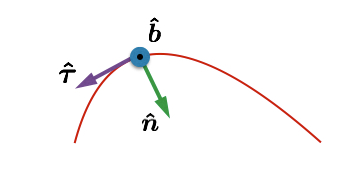
\includegraphics[height=1.9in,width=3.5in]{VOLUMEN_1/05_Analisis_Vectorial/Figuras/Figura5_0.jpg}
\caption{La tr�ada de vectores unitarios $\{ { \boldsymbol {\hat \tau}}, { \boldsymbol {\hat n}}, { \boldsymbol {\hat b}} \}$ para una curva en el plano.}
\label{Triada}
\end{center}
\end{figure}
%%%%%%%%%%%%%%%%%
A $\kappa$ se le denomina la {\it curvatura} de la curva $\Gamma$ y a la cantidad $\rho=1/\kappa$ {\it radio de curvatura}. De manera intuitiva, la curvatura nos indica que lejos est� una curva de ser una linea recta. 
\index{Curvatura}

Con este par de vectores coplanares se puede construir un tercero perpendicular tanto a ${ \boldsymbol {\hat \tau}}$ como a ${ \boldsymbol {\hat n}}$, que denominaremos vector {\it binormal} a  $\Gamma$, esto es: ${ \boldsymbol {\hat b}}={ \boldsymbol {\hat \tau }}\times { \boldsymbol {\hat n}}$. Tenemos entonces la tr�ada $\{ { \boldsymbol {\hat \tau}}, { \boldsymbol {\hat n}}, { \boldsymbol {\hat b}} \}$ al que podemos anclar un sistema de coordenadas cartesiano en cada punto de $\Gamma$. Es claro que este conjunto de vectores ir� cambiando a medida que $\mathbf{r}$ va cambiando al variar el par�metro. Este sistema de coordenadas, no inercial, estar� rotando constantemente a medida que el observador se mueve a lo largo de la curva en el espacio.

Continuando con el razonamiento anterior, por ser 
${ \boldsymbol {\hat b}} $ de magnitud constante, entonces
\[
{ \boldsymbol {\hat b}} \perp 
\frac{\mathrm{d}{ \boldsymbol {\hat b}}}{\mathrm{d}s}  
\quad \wedge \quad \frac{\mathrm{d}{ \boldsymbol {\hat b}}}{\mathrm{d}s}
\perp { \boldsymbol {\hat \tau}}
\]
Al ser ${\mathrm{d}{ \boldsymbol {\hat b}}}/{\mathrm{d}s} $  perpendicular tanto a ${ \boldsymbol {\hat \tau}}$ como a ${ \boldsymbol {\hat b}}$, entonces ser� proporcional a ${ \boldsymbol {\hat n}}$:
\[
\frac{\mathrm{d}{ \boldsymbol {\hat b}}}{\mathrm{d}s} =-\tau
{ \boldsymbol {\hat n}} \quad \Rightarrow  
\tau=-{ \boldsymbol {\hat n}}\cdot \frac{\mathrm{d}{ \boldsymbol {\hat b}}}{\mathrm{d}s} \,,
\]
esta constante de proporcionalidad se denomina la {\it torsi�n} de la curva $\Gamma$ en un punto dado, y a $1/\tau$ el radio de torsi�n. Intuitivamente, la {\it torsi�n} mide que lejos est� una curva de permanecer en un plano. 
\index{Torsi�n}


Para finalizar, a partir del hecho de que ${ \boldsymbol {\hat n}}={ \boldsymbol {\hat b}}\times { \boldsymbol {\hat \tau}}$:
\[
\frac{\mathrm{d}{ \boldsymbol {\hat n}}}{\mathrm{d}s}= 
\frac{\mathrm{d}{ \boldsymbol {\hat b}}}{\mathrm{d}s}\times
 { \boldsymbol {\hat \tau}} +
  { \boldsymbol {\hat b}} \times
\frac{\mathrm{d}{ \boldsymbol {\hat \tau}}}{\mathrm{d}s}=
-\tau({ \boldsymbol {\hat n}}\times { \boldsymbol {\hat \tau}})+
 \kappa ({ \boldsymbol {\hat b}} \times   { \boldsymbol {\hat n}})=
 \tau { \boldsymbol {\hat b}}-\kappa { \boldsymbol {\hat \tau}}\,.
\]
A las ecuaciones
\[
\frac{\mathrm{d}{ \boldsymbol {\hat \tau}}}{\mathrm{d}s}= 
\kappa { \boldsymbol {\hat n}} \,,\quad 
\frac{\mathrm{d}{ \boldsymbol {\hat b}}}{\mathrm{d}s} =-\tau
{ \boldsymbol {\hat n}}\,,\quad
\frac{\mathrm{d}{ \boldsymbol {\hat n}}}{\mathrm{d}s}=
 \tau { \boldsymbol {\hat b}}-\kappa { \boldsymbol {\hat \tau}}\,.
\]
se les conoce como las f�rmulas de Frenet-Serret de la geometr�a diferencial. 
\index{Frenet-Serret!F�rmulas de}

\subsection{Covectores, tensores y coordenadas curvil�neas}
\label{TensoresCurvilineos}
\index{Coordenadas curvil�neas!Tensores}
\index{Tensor!Coordenadas curvil�neas}
\index{Covector!Coordenadas curvil�neas}
Retomemos los conceptos que expresamos en la secci�n \ref{VectoresLeyesTransformacion}, de tal forma que podemos expresar vectores y formas como 
\[
\left| a \right> = a^i \left|  \mathrm{e}_{i}\right> =  a^x \left|  \mathrm{e}_{x}\right> + a^y \left|  \mathrm{e}_{y}\right> +  a^z \left|  \mathrm{e}_{z}\right> \equiv a^{\rho} \left|  \mathrm{e}_{\rho}\right> + a^{\varphi} \left|  \mathrm{e}_{\varphi}\right> +  a^z \left|  \mathrm{e}_{z}\right>
\] y equivalentemente para las 1-formas
\[
\left< a \right| = a^i \left<  \mathrm{e}_{i}\right| =  a^x \left<  \mathrm{e}_{x}\right| + a^y \left<  \mathrm{e}_{y}\right| +  a^z \left<  \mathrm{e}_{z}\right| \equiv a^{\rho} \left<  \mathrm{e}_{\rho}\right| + a^{\varphi} \left<  \mathrm{e}_{\varphi}\right| +  a^z \left<  \mathrm{e}_{z}\right| \, ,
\] en ambos casos hemos hecho la comparaci�n entre un sistema de coordenadas cartesiana y uno cil�ndrico. Lo que es importante notar es lo que insistimos en la secci�n \ref{VectoresLeyesTransformacion}, que los vectores y 1-formas, se expresan de forma equivalente en los distintos sistemas de coordenadas. 

Siguiendo la misma l�gica argumental que en la secci�n \ref{ProductoTensorial} construimos tensores en cualquier sistema de coordenadas curvil�neo a partir del producto tensorial de vectores y formas:
\[
\mathcal{T} = T^{i j} \left|  \mathrm{e}_{i}\right> \otimes \left|  \mathrm{\tilde{e}}_{j}\right> \equiv 
T_{i}^{j} \left<  \mathrm{e}^{i}\right| \otimes \left|  \mathrm{\tilde{e}_{j}}\right> \equiv
 T_{i j} \left<  \mathrm{e}^{i}\right| \otimes \left<  \mathrm{\tilde{e}^{j}}\right|\, .
\]Es importante recalcar que el tensor $\mathcal{T}$ es un objeto geom�trico que se expresa en una base (tensorial) particular y que las base de vectores $\left\{ \left|  \mathrm{e}_{i}\right>  \right\}$ y 1-formas $\left\{ \left<  \mathrm{\tilde{e}^{j}}\right| \right\}$, en principio, no necesariamente pueden ser las mismas, vale decir:
\[
\mathcal{T} = T^{x \rho} \left| \mathrm{e}_{x}; \mathrm{e}_{\rho} \right> + T^{x \varphi} \left| \mathrm{e}_{x}; \mathrm{e}_{\varphi} \right> + T^{x z} \left| \mathrm{e}_{x}; \mathrm{e}_{z} \right> + T^{y \rho} \left| \mathrm{e}_{y}; \mathrm{e}_{\rho} \right> + T^{y \varphi} \left| \mathrm{e}_{y}; \mathrm{e}_{\varphi} \right> + T^{y z} \left| \mathrm{e}_{y}; \mathrm{e}_{z} \right> + \cdots + T^{z z} \left| \mathrm{e}_{z}; \mathrm{e}_{z} \right> \, ,
\]donde hemos desarrollado el caso particular de un tensor bizarro parte cartesiano y parte cil�ndrico. Este tipo de objetos es solo un ejemplo. N�tese que estamos utilizando la notaci�n $\left| \mathrm{e}_{i}; \mathrm{e}_{j} \right> \equiv \left|  \mathrm{e}_{i}\right> \otimes \left|  \tilde{\mathrm{e}_{j}}\right>$. 
 
Solo para fijar ideas vamos a extender algunos conceptos que presentamos en la secci�n \ref{ProductoEscalar2}: 
\subsubsection{Producto escalar}
\label{ProductoEscalarCurvilineo}
\index{Coordenadas curvil�neas!Producto escalar}
\index{Producto escalar!Coordenadas curvil�neas}
El producto escalar es independiente de la base en la cual se exprese
\[
\left<a\right| \left. b\right> = a_{i}b^{i} = \tilde{a}_{j}\tilde{b}^{j}  = g_{ij} a^{i}b^{j} = \tilde{g}_{ij} \tilde{a}^{i}\tilde{b}^{j}  \, 
\]donde, como es de esperar, las leyes de transformaci�n entre el sistema de coordenadas cartesianas $x^{i} = x^{i}(q^{j})$ y un sistema de coordenadas curvil�neas $q^{j} = q^{j}(x^{i})$ permiten la traducci�n de las componentes de vectores, formas y tensores como:
\[
b^{i} = \frac{\partial x^{i}}{\partial q^{k}} \tilde{b}^{k}, \quad a_{j} = \frac{\partial q^{k}}{\partial x^{j}}\tilde{a}_{k}, \quad \mathrm{y} \quad g_{ij} = \frac{\partial q^{k}}{\partial x^{i}}\frac{\partial q^{m}}{\partial x^{j}} \tilde{g}_{km} 
\]
\subsubsection{Producto vectorial}
\label{ProductoVectorialCurvilineo}
\index{Coordenadas curvil�neas!Producto vectorial}
\index{Producto vectorial!Coordenadas curvil�neas}
El producto vectorial tal y como lo construimos la secci�n \ref{ProductoVectorial} se expresa como
\[
\left|c\right> = c^{i}\left|\mathrm{e}_{i}\right> = \left|a\right> \times \left|b\right>    = \epsilon^{ijk}a_{j}b_{k} \left|\mathrm{e}_{i}\right>  \quad \Leftrightarrow \quad \left|\tilde{c}\right> =  \tilde{c}^{i}\left|\mathrm{\tilde{e}}_{i}\right> = 
\left|\tilde{a}\right> \times \left|\tilde{b}\right>  = \tilde{\epsilon}^{ijk}\tilde{a}_{j}\tilde{b}_{k}  \left|\mathrm{\tilde{e}}_{i}\right> \, .
\]Donde $\epsilon^{ijk}$ es el tensor de Levi-Civita en coordenadas cartesianas definido en la secci�n \ref{ConvencionEinstein} y que luego generalizamos en la secci�n \ref{Determinante}.  Es decir, queremos construir la versi�n del producto vectorial que tenga la misma forma que en el caso cartesiano pero en cualquier sistema de coordenadas. De la relaci�n anterior es claro que, el tensor de Levi-Civita transformar� como un tensor, es decir 
\[
\tilde{\epsilon}^{ijk} = \epsilon^{lmn} \frac{\partial q^{i} }{\partial x^{l}} \frac{\partial q^{j} }{\partial x^{m}} \frac{\partial q^{k} }{\partial x^{n}} = J \, \epsilon^{ijk} = \sqrt{g} \, \epsilon^{ijk}
\]donde $J$ es el determinante de la matriz jacobiana, que discutimos en \ref{TransformacionCoordenadas} y $g$ el determinante de la m�trica. 
\index{Levi-Civita!Tensor}
\index{Tensor!Levi-Civita} 
\index{Jacobiano}
\index{Matriz!Jacobiana}
Por lo tanto,
\[
\left|c\right> = \left|a\right> \times \left|b\right>  = a_{j}b_{k} \epsilon^{ijk} \left|\mathrm{e}_{i}\right> = 
\epsilon^{ijk} \left(\tilde{a}_{l} \frac{\partial q^{l}}{\partial x^{j} }\right) \left(\tilde{b}_{m} \frac{\partial q^{m}}{\partial x^{k} } \right) \left( \frac{\partial q^{n}}{\partial x^{i} }\left|\mathrm{\tilde{e}}_{n}\right>\right) = 
\left( \epsilon^{ijk} \frac{\partial q^{l}}{\partial x^{j} } \frac{\partial q^{m}}{\partial x^{k} } \frac{\partial q^{n}}{\partial x^{i} } \right) \tilde{a}_{l} \tilde{b}_{m} \left|\mathrm{\tilde{e}}_{n}\right> \, ,
\]con lo cual
\[
\left|c\right> = \left|a\right> \times \left|b\right> = \underbrace{a_{j}b_{k} \epsilon^{ijk}}_{c^{i}} \left|\mathrm{e}_{i}\right> =
\underbrace{\tilde{a}_{m}\tilde{b}_{n} \tilde{\epsilon}^{lmn}}_{\tilde{c}^{l}} \left|\mathrm{\tilde{e}}_{l}\right>    
= J \, \epsilon^{lmn} \tilde{a}_{m}\tilde{b}_{n} \left|\mathrm{\tilde{e}}_{l}\right> =  
\sqrt{g} \, \epsilon^{lmn} \tilde{a}_{m}\tilde{b}_{n} \left|\mathrm{\tilde{e}}_{l}\right>
\]

\subsection{{\color{Fuchsia}Ejemplos}}
\begin{enumerate}
\item \textbf{Velocidades y aceleraciones. }
Para fijar conceptos repasaremos los c�lculos de las expresiones de las velocidades y las aceleraciones, que expusimos en la secci�n \ref{VelocidadesAceleraciones3D}, solo que ahora los desarrollaremos en coordenadas generalizadas. Para ello recordamos que los vectores velocidad y aceleraci�n se representan como
\[
\left| v \right> =v^{j} \left|  \mathrm{e}_{j}\right>  =\dot{x}^{j} \left| \mathrm{e}_{j}\right> = 
\tilde{v}^{j} \left|  \mathrm{\tilde{e}}_{j}\right>  = \dot{\tilde{x}}^{j} \left|  \mathrm{\tilde{e}}_{j}\right> \quad \mathrm{y} \quad
\left|  a \right> =
a^{j} \left|  \mathrm{e}_{j}\right>  =\ddot{x}^{j} \left|  \mathrm{e}_{j}\right> = \tilde{a}^{j} \left|  \mathrm{\tilde{e}}_{j}\right>  = \ddot{\tilde{x}}^{j} \left|  \mathrm{\tilde{e}}_{j}\right> \,,
\]
respectivamente. 

Para determinar  estos vectores en cualquier sistema de coordenadas, es suficiente con encontrar las expresiones de sus componentes covariantes o contravariantes. Como sabemos, podremos encontrar una a partir de las otras con la ayuda de la m�trica del sistema de coordenadas.

Entonces, el vector velocidad en la base cartesiana se puede expresar como
\[
\left|v \right> = v_{x} \left| \mathrm{e}_{x}\right> + v_{y} \left| \mathrm{e}_{y}\right> + v_{z} \left| \mathrm{e}_{z}\right> = \dot{x} \left| \mathrm{e}_{x}\right> + \dot{y} \left| \mathrm{e}_{y}\right> + \dot{z} \left| \mathrm{e}_{z}\right> =
\dot{x}^{j} \left|  \mathrm{e}_{j}\right> \,,
\]
con: $\left|  \mathrm{e}_{1}\right> =  \left| \mathrm{e}_{x}\right>, 
\left|  \mathrm{e}_{2}\right> =  \left| \mathrm{e}_{y}\right> \quad \mathrm{y} \quad 
 \left| \mathrm{e}_{3}\right> =  \left| \mathrm{e}_{z}\right>$.
 
Claramente las componentes contravariantes del vector velocidad en un sistema de coordenadas generalizado son $ v^{j}=\dot{q}^{j} $.

Recordamos que para cualquier base generalizada de vectores o formas las componentes covariantes se expresan en t�rmino de la base cartesiana (de vectores o formas) como
\[
\left|  \mathrm{\tilde{e}}_{j}\right> =\frac{\partial x^{i}}{\partial q^{j}} \left|  \mathrm{e}_{i}\right> \quad \mathrm{y} \quad
\left<  \mathrm{\tilde{e}}^{i} \right| =\frac{\partial q^{i}}{\partial x^{j}} 
\left<  \mathrm{e}^{j} \right|\,.
\] 

Entonces, las componentes covariantes del vector velocidad en una base generalizada ser�n
\[
\tilde{v}_{j} =  \left<  v \right. \left|  \mathrm{\tilde{e}}_{j}\right> = \left( \dot{x}_{m} \left<  \mathrm{\tilde{e}}^{m} \right|  \right) \left(  \frac{\partial x^{i}}{\partial q^{j}} \left|  \mathrm{e}_{i}\right> \right) = 
\dot{x}_{m}  \frac{\partial x^{m}}{\partial q^{j}} = \dot{x}_{m}  \frac{ \frac{\partial x^{m}}{\partial t}}{\frac{\partial q^{j}}{\partial t}} = \dot{x}_{m}  \frac{\partial \dot{x}^{m}}{\partial \dot{q}^{j}} =   \frac{\partial\left(\frac{ v_{m} v^{m} }{2} \right)}{\partial \dot{q}^{j}}\,.
\]

Resulta f�cil expresar las componentes covariantes una vez que conocemos el m�dulo del vector expresado en ese sistema de coordenadas, el cual siempre viene escrito a partir del diferencial 
\[ 
\mathrm{d}\left| {r} \right> \quad \Rightarrow  
\frac{\mathrm{d}\left|  {r} \right> }{\mathrm{d}t} \,.
\]

Para encontrar la expresi�n para la aceleraci�n se procede de manera an�loga. 
\[
\tilde{a}_{j} =  \left<  a \right. \left|  \mathrm{\tilde{e}}_{j}\right> = \left( \ddot{x}_{m} \left<  \mathrm{\tilde{e}}^{m} \right|  \right) \left(  \frac{\partial x^{i}}{\partial q^{j}} \left|  \mathrm{e}_{i}\right> \right) = 
\ddot{x}_{m}  \frac{\partial x^{m}}{\partial q^{j}} \equiv \frac{\mathrm{d}}{\mathrm{d}t}\left( \dot{x}_{m}  \frac{\partial x^{m}}{\partial q^{j}}   \right) - \dot{x}_{m}  \frac{\partial \dot{x}^{m}}{\partial q^{j}} \,,
\]
y otra vez
\[
 \frac{\partial x^{m}}{\partial q^{j}} =  \frac{\partial \dot{x}^{m}}{\partial \dot{q}^{j}} \quad \Rightarrow 
 \tilde{a}_{j} = \frac{\mathrm{d}}{\mathrm{d}t}\left( \dot{x}_{m}  \frac{\partial \dot{x}^{m}}{\partial \dot{q}^{j}}   \right) - \dot{x}_{m}  \frac{\partial \dot{x}^{m}}{\partial q^{j}} =  \frac{\mathrm{d}}{\mathrm{d}t}\left[ \frac{\partial }{\partial \dot{q}^{j}}\left(\frac{ \dot{x}_{m} \dot{x}^{m} }{2} \right)   \right] -  \frac{\partial }{\partial q^{j}}\left(\frac{ \dot{x}_{m} \dot{x}^{m} }{2} \right) \,,
\]
para finalmente
\[
 \tilde{a}_{j} =  \frac{\mathrm{d}}{\mathrm{d}t}\left[ \frac{\partial }{\partial \dot{q}^{j}}\left(\frac{ v_{m}v^{m} }{2} \right)   \right] -  \frac{\partial }{\partial q^{j}}\left(\frac{ v_{m} v^{m} }{2} \right)\,.
\]


\item Calculemos las componentes cartesianas del vector que, en coordenadas cil�ndricas, tiene las siguiente componentes: 
$\left(1,\pi/3,3\right) $.


Ese vector en coordenadas cil�ndricas se puede escribir como: 
${\bf V}=\left|  \mathrm{e}_{r}\right> +\frac{\pi}{3}\left|  \mathrm{e}_{\varphi}\right> + 3\left|  \mathrm{e}_{z}\right> $. En general, las componentes de los vectores transforman como
\[
\tilde{a}^{i}=\dfrac{\partial \tilde{x}^{i}\left(x^{m}\right)  }
{\partial x^{k}}\ a^{k}\quad \Rightarrow  \left\{
\begin{array}
[c]{c}
\tilde{a}^{1}=\dfrac{\partial \tilde{x}^{1}\left(  x^{m}\right)  }
{\partial x^{k}}\ a^{k}\\
\\
\tilde{a}^{2}=\dfrac{\partial \tilde{x}^{2}\left(  x^{m}\right)  }
{\partial x^{k}}\ a^{k}\\
\\
\tilde{a}^{3}=\dfrac{\partial \tilde{x}^{3}\left(  x^{m}\right)  }
{\partial x^{k}}\ a^{k}
\end{array}
\right\}  \quad\text{con }\left\{
\begin{array}
[c]{c}
\tilde{x}^{1}=x\\
\\
\tilde{x}^{2}=y\\
\\
\tilde{x}^{3}=z
\end{array}
\right\}  \quad\text{y}\quad\left\{
\begin{array}
[c]{c}
x^{1}=r\\
\\
x^{2}=\varphi\\
\\
x^{3}=z
\end{array}
\right\}
\]
y la ley de transformaci�n entre coordenadas cartesianas y coordenadas cil�ndricas es
\[
x=x\left(  r,\varphi\right)  =r\cos(\varphi);\quad 
y=y\left(r,\varphi\right)=r\mathrm{sen}(\varphi)\quad\text{y}\quad z=z \,,
\]
con lo cual es f�cil identificar
\[
\begin{array}
[c]{c}
\frac{\partial x\left(  r,\varphi\right)  }{\partial r}=\cos(\varphi)\\
\\
\frac{\partial y\left(  r,\varphi\right)  }{\partial r}=
\mathrm{sen}
(\varphi)\\
\\
\frac{\partial z}{\partial r}=0
\end{array}
 \qquad
\begin{array}
[c]{c}
\frac{\partial x\left(  r,\varphi\right)  }{\partial \varphi}
=-r
\mathrm{sen}(\varphi)\\
\\
\frac{\partial y\left(  r,\varphi\right)  }{\partial \varphi}=r\cos(\varphi)\\
\\
\frac{\partial z}{\partial \varphi}=0
\end{array}
\qquad
\begin{array}
[c]{c}
\frac{\partial x\left(  r,\varphi\right)  }{\partial z}=0\\
\\
\frac{\partial y\left(  r,\varphi\right)  }{\partial z}=0\\
\\
\frac{\partial z}{\partial z}=1
\end{array}
\]

Por lo tanto
\begin{align*}
\tilde{a}^{1} &  =\dfrac{\partial \tilde{x}^{1}\left(  x^{m}\right)}{\partial x^{k}}\ a^{k}=
\dfrac{\partial \tilde{x}^{1}\left(  x^{m}\right)}{\partial x^{1}}\ a^{1}+\dfrac{\partial \tilde{x}^{1}\left(  x^{m}\right)}{\partial x^{2}}\ a^{2}+\dfrac{\partial \tilde{x}^{1}\left(  x^{m}\right)}{\partial x^{3}}\ a^{3}\\
& \\
\tilde{a}^{1} &  =\frac{\partial x\left(r,\varphi\right)  }{\partial r}\left(1\right) + \frac{\partial x\left(r,\varphi\right)}
{\partial \varphi}\left(\frac{\pi}{3}\right)  =\cos(\varphi)-r\mathrm{sen}(\varphi)\left(\frac{\pi}{3}\right)=\cos\left(\frac{\pi}{3} \right)  -(1)\mathrm{sen}\left( \frac{\pi}{3}\right)\left(\frac{\pi}{3}\right) =
\frac{\sqrt{3}-\pi}{2\sqrt{3}} \,,
\end{align*}
del mismo modo
\begin{align*}
\tilde{a}^{2} &  =\frac{\partial y\left(  r,\varphi\right)  }{\partial r}\left(1\right)  +\frac{\partial y\left(  r,\varphi\right)  }
{\partial \varphi}\left(\frac{\pi}{3}\right)  =\mathrm{sen}(\varphi)+
r\cos(\varphi)\left(\frac{\pi}{3}\right)=\mathrm{sen}\left(\frac{\pi}{3}\right)  +\left(  1\right)  \cos\left(  \frac{\pi}{3}\right)\left(\frac{\pi}{3}\right)  =\frac{\sqrt{27}+\pi}{6} \,, \\
& \\
\tilde{a}^{3} &  =3 \,.
\end{align*}

Con lo cual 
\[
{\bf V}=\left|  \mathrm{e}_{r}\right> +\frac{\pi}{3}\left|  \mathrm{e}_{\varphi}\right> + 3\left|  \mathrm{e}_{z}\right> =
\frac{\sqrt{3}-\pi}{2\sqrt{3}}\ \left|{\mathrm{i}}\right> +\frac{\sqrt{27}+\pi}{6}\ \left|{\mathrm{j}}\right> +3\ \left|{\mathrm{k}}\right> \,.
\]

\item Dado el siguiente vector en coordenadas cil�ndricas 
 ${\bf a}=-2\left|  \mathrm{e}_{\rho}\right> +5\left|  \mathrm{e}_{\tilde{\varphi}}\right> +4\left|  \mathrm{e}_{z}\right>$. Vamos a ver como queda expresado en coordenadas esf�ricas.

La primera forma de hacerlo es transformando las componentes al conocer como transforman las coordenadas. Es decir conociendo $x^{i}=x^{i}\left(  \tilde{x}^{m}\right)  $ y $\tilde{x}^{j}=\tilde{x}^{j}\left( x^{m}\right)  $ {expresar} $\tilde{a}^{i}=
\frac{\partial \tilde{x}^{i}}{\partial x^{k}}\ a^{k}$. Dado que
\begin{eqnarray*}
x\left( \rho,\tilde{\varphi}\right) &=&\rho\cos(\tilde{\varphi})= x\left(r,\varphi,\theta\right)=r\cos(\varphi)\mathrm{sen}(\theta) \\
y\left( \rho,\tilde{\varphi}\right) &=&\rho\mathrm{sen}(\tilde{\varphi})= y\left(r,\varphi,\theta\right)=r\mathrm{sen}(\varphi)\mathrm{sen}(\theta)\\
z&=& z = r\cos(\theta) \,.
\end{eqnarray*}
Por lo tanto:
\[
\rho=r\mathrm{sen}(\theta)\,, \quad \tilde{\varphi}=\varphi \,,\quad z=r\cos(\theta) \quad \Rightarrow   
r=\sqrt{\rho^{2}+z^{2}};\quad\theta=\arctan\left(  \frac{\rho}{z}\right)\,;
\quad\tilde{\varphi}=\varphi \,.
\]

En forma matricial:
\begin{eqnarray*}
\tilde{a}^{i}  & =& \frac{\partial \tilde{x}^{i}}{\partial x^{k}}\ a^{k}=
\left(
\begin{array}
[c]{ccc}
\frac{\partial \tilde{x}^{1}}{\partial x^{1}} & \frac{\partial \tilde{x}^{1}}{\partial x^{2}} & \frac{\partial \tilde{x}^{1}}{\partial x^{2}}\\ \\
\frac{\partial \tilde{x}^{2}}{\partial x^{1}} & \frac{\partial \tilde{x}^{2}}{\partial x^{2}} & \frac{\partial \tilde{x}^{2}}{\partial x^{3}}\\ \\
\frac{\partial \tilde{x}^{3}}{\partial x^{1}} & \frac{\partial \tilde{x}^{3}}{\partial x^{2}} & \frac{\partial \tilde{x}^{3}}{\partial x^{3}}
\end{array}
\right)  \left(
\begin{array}
[c]{c}
-2\\
5\\
4
\end{array}
\right)  =\left(
\begin{array}
[c]{ccc}
\frac{\partial r}{\partial \rho} & \frac{\partial r}{\partial \varphi} & \frac{\partial r}{\partial z}\\ \\
\frac{\partial \varphi}{\partial \rho} & \frac{\partial \varphi}{\partial \varphi} & \frac{\partial \varphi}{\partial z}\\ \\
\frac{\partial \theta}{\partial \rho} & \frac{\partial \theta}{\partial \varphi} & \frac{\partial \theta}{\partial z}
\end{array}
\right)  \left(
\begin{array}
[c]{c}
-2\\
5\\
4
\end{array}
\right)  \\
& = &
\left(
\begin{array}
[c]{ccc}
\frac{\partial \sqrt{\rho^{2}+z^{2}}}{\partial \rho} & \frac{\partial\ \sqrt{\rho^{2}+z^{2}}}{\partial \varphi} & \frac{\partial \sqrt{\rho
^{2}+z^{2}}}{\partial z}\\ \\
0 & 1 & 0 \\ \\
\frac{\partial \arctan\left(  \frac{\rho}{z}\right)  }{\partial \rho} & \frac{\partial \arctan\left(  \frac{\rho}{z}\right)  }{\partial \varphi} &
\frac{\partial \arctan\left(  \frac{\rho}{z}\right)  }{\partial z}
\end{array}
\right)  \left(
\begin{array}
[c]{c}
-2\\
5\\
4
\end{array}
\right)  =\left(
\begin{array}
[c]{ccc}
\frac{\rho}{\sqrt{\rho^{2}+z^{2}}} & 0 & \frac{z}{\sqrt{\rho^{2}+z^{2}}}\\
0 & 1 & 0\\
\frac{z}{\rho^{2}+z^{2}} & 0 & \frac{-\rho}{\rho^{2}+z^{2}}
\end{array}
\right)  \left(
\begin{array}
[c]{c}
-2\\
5\\
4
\end{array}
\right) \,.
\end{eqnarray*}

Resultando, que en esf�ricas
\[
{\bf a}=\left(
\begin{array}
[c]{c}
-2\mathrm{sen}(\theta)+4\cos(\theta)\\
5\\
\frac{-2\cos(\theta)}{r}-\frac{4\ \mathrm{sen}(\theta)}{r}
\end{array}
\right)  =
\left( -2\mathrm{sen}(\theta)+4\cos(\theta)\right)
\left|\mathrm{e}_{r}\right> +
5 \left|\mathrm{e}_{\varphi}\right> -
\left(  \frac{2\cos(\theta)}{r}+\frac{4\mathrm{sen}(\theta)}{r}\right) 
\left|\mathrm{e}_{\theta}\right> \,.
\]

La otra forma es expresar la base ortonormal cil�ndrica en
t�rminos de la base ortonormal esf�rica. Otra vez, utilizamos la base
cartesiana como intermediaria. Esto es:
\[
\left.
\begin{array}
[c]{l}
\left|\mathrm{e}_{\rho}\right> =
\cos(\tilde{\varphi})\left|{\mathrm{i}}\right>+
\mathrm{sen}(\tilde{\varphi}) \left|{\mathrm{j}}\right> \,, \\
\left|\mathrm{e}_{\tilde{\varphi}}\right> =
-\mathrm{sen}(\tilde{\varphi}) \left|{\mathrm{i}}\right>+
\cos(\tilde{\varphi}) \left|{\mathrm{j}}\right> \\
\left|\mathrm{e}_{z}\right> =\left|{\mathrm{k}}\right>
\end{array}
\right\}  \quad \Leftrightarrow\quad \left\{
\begin{array}
[c]{l}
\left|{\mathrm{i}}\right>=
\cos(\tilde{\varphi}) \left|\mathrm{e}_{\rho}\right> -
\mathrm{sen}(\tilde{\varphi}) \left|\mathrm{e}_{\tilde{\varphi}}\right>\\
\left|{\mathrm{j}}\right>=\mathrm{sen}(\tilde{\varphi}) 
\left|\mathrm{e}_{\rho}\right>
+\cos(\tilde{\varphi})\left|\mathrm{e}_{\tilde{\varphi}}\right> \\
\left|{\mathrm{k}}\right>=\left|\mathrm{e}_{z}\right>
\end{array}
\right.
\]

Mientras que  en esf�ricas, donde
\begin{eqnarray*}
\left|\mathrm{e}_{r}\right>&=&\cos(\varphi)\mathrm{sen}(\theta)
\left|{\mathrm{i}}\right>+\mathrm{sen}(\varphi)
\mathrm{sen}(\theta)\left|{\mathrm{j}}\right>+\cos(\theta)
\left|{\mathrm{k}}\right>\\
\left|\mathrm{e}_{\varphi}\right>&=&-\mathrm{sen}(\varphi)\ \left|{\mathrm{i}}\right>+\cos(\varphi)\left|{\mathrm{j}}\right> \\
\left|\mathrm{e}_{\theta}\right>&=&\cos(\varphi)\cos(\theta) \left|{\mathrm{i}}\right>+\mathrm{sen}(\varphi)\cos(\theta)\left|{\mathrm{j}}\right>-\mathrm{sen}(\theta)\left|{\mathrm{k}}\right>
\end{eqnarray*}
y 
\begin{eqnarray*}
\left|{\mathrm{i}}\right>&=&\cos(\varphi)\mathrm{sen}(\theta)
\left|\mathrm{e}_{r}\right>+\cos(\varphi)\cos(\theta)
\left|\mathrm{e}_{\theta}\right>-\mathrm{sen}(\varphi)
\left|\mathrm{e}_{\varphi}\right> \\
\left|{\mathrm{j}}\right>&=&\mathrm{sen}(\varphi)\mathrm{sen}(\theta)
\left|\mathrm{e}_{r}\right>+\mathrm{sen}(\varphi)\cos(\theta)\left|\mathrm{e}_{\theta}\right>+\cos(\varphi)
\left|\mathrm{e}_{\varphi}\right> \\
\left|{\mathrm{k}}\right>&=&\cos(\theta)\left|\mathrm{e}_{r}\right> -\mathrm{sen}(\theta)\left|\mathrm{e}_{\theta}\right>
\end{eqnarray*}

Con lo cual
\begin{eqnarray*}
\left|\mathrm{e}_{\rho}\right>  & =&\cos(\varphi)\left[  \cos(\varphi)\mathrm{sen}(\theta)\left|\mathrm{e}_{r}\right>
+\cos(\varphi)\cos(\theta)\left|\mathrm{e}_{\theta}\right> -\mathrm{sen}(\varphi)\left|\mathrm{e}_{\varphi}\right> \right] \\
&+&\mathrm{sen}(\varphi) \left[  \mathrm{sen}(\varphi)\mathrm{sen}(\theta) \left|\mathrm{e}_{r}\right>+\mathrm{sen}(\varphi)\cos(\theta)
\left|\mathrm{e}_{\theta}\right>+\cos(\varphi)
\left|\mathrm{e}_{\varphi}\right> \right]\\
& =&\mathrm{sen}(\theta)\left|\mathrm{e}_{r}\right>+\cos(\theta)
\left|\mathrm{e}_{\theta}\right>\\
\left|\mathrm{e}_{\varphi}\right> & =&\left|\mathrm{e}_{\varphi}\right> \\
\left|\mathrm{e}_{z}\right>  & =&\cos(\theta)\left|\mathrm{e}_{r}\right>-\mathrm{sen}(\theta)\left|\mathrm{e}_{\theta}\right>
\end{eqnarray*}
entonces
\[
{\bf a}=-2\left|\mathrm{e}_{\rho}\right>+
5\left|\mathrm{e}_{\varphi}\right>+4\left|\mathrm{e}_{z}\right>=-2\left(\mathrm{sen}(\theta)\left|\mathrm{e}_{r}\right>
+\cos(\theta) \left|\mathrm{e}_{\theta}\right> \right)
+5\left( \left|\mathrm{e}_{\varphi}\right>\right)  +4\left(  \cos(\theta)\left|\mathrm{e}_{r}\right>
-\mathrm{sen}(\theta)\left|\mathrm{e}_{\theta}\right>\right)
\]
Finalmente
\[
{\bf a}=\left( -2\mathrm{sen}(\theta)+4\cos(\theta)\right) 
\left|\mathrm{e}_{r}\right>+5\left|\mathrm{e}_{\varphi}\right>-\left( 2\cos(\theta)+4\mathrm{sen}(\theta)\right)  
\left|\mathrm{e}_{\theta}\right>\,.
\]

\item  Dado el sistema de coordenadas parab�licas
\[
x=\xi\eta\cos(\varphi);\qquad y=\xi\eta
\mathrm{sen}(\varphi);\qquad
z=\frac{1}{2}\left(  \eta^{2}-\xi^{2}\right)
\]

Vamos a calcular el diferencial de volumen $\mathrm{d}v=\mathrm{d}x \mathrm{d}y \mathrm{d}z$ en estas coordenadas



Hay varias maneras de resolver este problema. La m�s intuitiva es
que, dado que las coordenadas parab�licas son un sistema de coordenadas ortogonales entonces multiplicar largo, por ancho, por alto con las longitudes de arco en cada una de las direcciones ortogonales. Esto es
\[
\mathrm{d}s^{2}={g}_{nu}\mathrm{d}q^{n}\mathrm{d}q^{u}=
{g}_{11}\left(  \mathrm{d}q^{1}\right)^{2}+{g}_{22}\left(
\mathrm{d}q^{2}\right)^{2}+{g}_{33}\left(  \mathrm{d}q^{3}\right)
^{2}\quad \Rightarrow \left\{
\begin{array}
[c]{c}
\mathrm{d}s_{\rightarrow1}^{2}={g}_{11}\left(  \mathrm{d}q^{1}\right)
^{2}\\
\\
\mathrm{d}s_{\rightarrow2}^{2}={g}_{22}\left(  \mathrm{d}q^{2}\right)
^{2}\\
\\
\mathrm{d}s_{\rightarrow3}^{2}={g}_{33}\left(  \mathrm{d}q^{3}\right)
^{2}
\end{array}
\right.
\]
por consiguiente
\[
\mathrm{d}v=\left(  \mathrm{d}s_{\rightarrow1}\right)  \left(  \mathrm{d}
s_{\rightarrow2}\right)  \left(  \mathrm{d}s_{\rightarrow3}\right)
=\sqrt{{g}_{11}}\mathrm{d}q^{1}\sqrt{{g}_{22}}\mathrm{d}q^{2}
\sqrt{{g}_{33}}\mathrm{d}q^{3}=h_{1}h_{2}h_{3}\mathrm{d}q^{1}
\mathrm{d}q^{2}\mathrm{d}q^{3}
\]
con
\begin{align*}
h_{1} &  =\left\|  \frac{\partial   \mathbf{r} }{\partial q^{1}}\right\|  =
\sqrt{{g}_{11}}=\sqrt{\left(  \frac{\partial x\left(  q^{1},q^{2},q^{3}\right)  }{\partial q^{1}}\right)^{2}+\left(  \frac{\partial y \left(  q^{1},q^{2},q^{3}\right)  }{\partial q^{1}}\right)^{2}+\left(  \frac{\partial z\left(  q^{1}
,q^{2},q^{3}\right)  }{\partial q^{1}}\right)^{2}}\\
h_{2} &  =\left\|  \frac{\partial   \mathbf{r} }{\partial q^{2}}\right\|  =
\sqrt{{g}_{22}}=\sqrt{\left(  \frac{\partial x\left(  q^{1},q^{2},q^{3}\right)  }{\partial q^{2}}\right)^{2}+\left(  \frac{\partial y\left(  q^{1},q^{2},q^{3}\right)  }{\partial q^{2}}\right)^{2}+\left(  \frac{\partial z\left(  q^{1},q^{2},q^{3}\right)  }{\partial q^{2}}\right)^{2}}\\
h_{3} &  =\left\|  \frac{\partial  \mathbf{r} }{\partial q^{3}}\right\|  =
\sqrt{{g}_{11}}=\sqrt{\left(  \frac{\partial x\left(  q^{1},q^{2},q^{3}\right)  }{\partial q^{3}}\right)^{2}+\left(  \frac{\partial y\left(  q^{1},q^{2},q^{3}\right)  }{\partial q^{3}}\right)^{2}+\left(  \frac{\partial z\left(  q^{1},q^{2},q^{3}\right)  }{\partial q^{3}}\right)^{2}}
\end{align*}
por lo cual, dado que $ \mathbf{r} =x\left(  \eta,\xi,\varphi\right)    \mathbf{i} +y\left(  \eta
,\xi,\varphi\right)  \mathbf{j} +z\left(  \eta ,\xi\right)   \mathbf{k} $, entonces
\begin{align*}
h_{1} &  =\left\|  \frac{\partial  \mathbf{r} }{\partial q^{1}}\right\|  =
\sqrt{{g}_{11}}=\sqrt{\left(  \eta\cos(\varphi)\right)^{2}+\left(  \eta
\mathrm{sen}(\varphi)\right)^{2}+\left(
\xi\right)^{2}}=\sqrt{\left(  \eta^{2}+\xi^{2}\right)  }\\
h_{2} &  =\left\|  \frac{\partial  \mathbf{r} }{\partial q^{2}}\right\|  =
\sqrt{{g}_{22}}=\sqrt{\left(  \xi\cos\varphi\right)^{2}+\left(  \xi
\mathrm{sen}(\varphi)\right)^{2}+\left(  -\eta\right)^{2}}=
\sqrt{\left(  \eta^{2}+\xi^{2}\right)  }\\
h_{1} &  =\left\|  \frac{\partial   \mathbf{r} }{\partial q^{1}}\right\|  =\sqrt{{g}_{11}}=\sqrt{\left(  -\xi \eta \mathrm{sen}(\varphi)\right)^{2}+\left(  \xi\eta\cos(\varphi)\right)^{2} +\left(0\right)^{2}}=\xi\eta
\end{align*}
y finalmente
\[
\mathrm{d}v=h_{1}h_{2}h_{3}\mathrm{d}\xi\mathrm{d}\eta\mathrm{d}\varphi
=\xi\eta\left(  \eta^{2}+\xi^{2}\right)  \mathrm{d}\xi\mathrm{d}\eta
\mathrm{d}\varphi \,.
\]

La otra forma de resolverlo, tambi�n intuitiva, es hacer el producto mixto de los tres vectores ortogonales base sin normalizar. Esto es
\[
\mathrm{d}v=\left\|  \left(  \mathrm{d}q^{1}\frac{\partial 
\mathbf{r}}{\partial q^{1}}\right)  \cdot  \left(
\mathrm{d}q^{2}\frac{\partial  \mathbf{r} }
{\partial q^{2}}\times\mathrm{d}q^{3}\frac{\partial  \mathbf{r}}
{\partial q^{3}}\right)  \right\|  =\mathrm{d}q^{1}
\mathrm{d}q^{2}\mathrm{d}q^{3}\left\|  \frac{\partial \mathbf{r}
 }{\partial q^{1}}\cdot \left(  \frac{\partial 
\mathbf{r} }{\partial q^{2}}\times\frac{\partial
\mathbf{r} }{\partial q^{3}}\right)  \right\| \,.
\]

En general
\begin{align*}
\mathrm{d}v &  =\mathrm{d}q^{1}\mathrm{d}q^{2}\mathrm{d}q^{3}
\left[
\det\left|
\begin{array}
[c]{ccc}
\frac{\partial x\left(  q^{1},q^{2},q^{3}\right)  }{\partial q^{1}} &
\frac{\partial y\left(  q^{1},q^{2},q^{3}\right)  }{\partial q^{1}} &
\frac{\partial z\left(  q^{1},q^{2},q^{3}\right)  }{\partial q^{1}}\\
\frac{\partial x\left(  q^{1},q^{2},q^{3}\right)  }{\partial q^{2}} &
\frac{\partial y\left(  q^{1},q^{2},q^{3}\right)  }{\partial q^{2}} &
\frac{\partial z\left(  q^{1},q^{2},q^{3}\right)  }{\partial q^{2}}\\
\frac{\partial x\left(  q^{1},q^{2},q^{3}\right)  }{\partial q^{3}} &
\frac{\partial y\left(  q^{1},q^{2},q^{3}\right)  }{\partial q^{3}} &
\frac{\partial z\left(  q^{1},q^{2},q^{3}\right)  }{\partial q^{3}}
\end{array}
\right|  \right]  \\
& \\
&  =\mathrm{d}q^{1}\mathrm{d}q^{2}\mathrm{d}q^{3}\det\left| J\left(  x\left(
q^{1},q^{2},q^{3}\right)  ,y\left(  q^{1},q^{2},q^{3}\right)  ,z\left(
q^{1},q^{2},q^{3}\right)  \right)  \right|
\end{align*}
donde $J\left(  x\left(  q^{1},q^{2},q^{3}\right)  ,y\left(  q^{1},q^{2}
,q^{3}\right)  ,z\left(  q^{1},q^{2},q^{3}\right)  \right) $ es la matriz Jacobiana de la transformaci�n. 
\index{Jacobiano}

Entonces
\[
\mathrm{d}v=\mathrm{d}\xi\mathrm{d}\eta\mathrm{d}\varphi\left(  
\det\left|
\begin{array}
[c]{ccc}%
\eta\cos(\varphi) & \eta \ \mathrm{sen}(\varphi) & \xi \\
\xi \cos(\varphi) & \xi \ \mathrm{sen}(\varphi) & -\eta \\
-\xi\eta \ \mathrm{sen}(\varphi) & \xi\eta\cos(\varphi) & 0
\end{array}
\right|  \right)  =\xi\eta\left(  \eta^{2}+\xi^{2}\right)  \mathrm{d}\xi\mathrm{d}\eta\mathrm{d}\varphi
\]

En general, el diferencial del volumen viene expresado como un producto mixto de la base ortonormal $\left\{  \left|  \mathrm{q}_{1}\right> ,\left|  \mathrm{q}_{2}\right> ,\left|  \mathrm{q}_{3}\right> \right\}  $
\begin{align*}
\mathrm{d}v &  = \left\|  \left(  \mathrm{d}q^{1} \left|  \mathrm{q}_{1} \right> \right)  \cdot \left(  \mathrm{d}q^{2} \left| \mathrm{q}_{2} \right> \times \mathrm{d}q^{3} \left|  \mathrm{q}_{3}\right> \right)  \right\|  =
\mathrm{d}q^{1}\mathrm{d}q^{2} \mathrm{d}q^{3} \left\|  \left|  \mathrm{q}_{1}\right> \cdot \left( \left|  \mathrm{q}_{2}\right> \times\left|  \mathrm{q}_{3}\right> \right)  \right\|  \\ & \\
\mathrm{d}v &  =\mathrm{d}q_{n}\left< \mathrm{q}^{n}\right|  \left( \epsilon^{123} \mathrm{d}q_{2}\mathrm{d}q_{3}\left|  \mathrm{q}_{1}\right> \right)  =  g_{nu}\mathrm{d}q^{u} g_{22}\mathrm{d}q^{2} g_{33}\mathrm{d}q^{3} \underset{\delta_{1}^{n}}{\underbrace{\left< \mathrm{q}^{n}\right.  \left|  \mathrm{q}_{1}\right> }}=
g_{11}\mathrm{d}q^{1} g_{22} \mathrm{d}q^{2} g_{33}\mathrm{d}q^{3} \,.
\end{align*}


\item Para una curva en el plano $xy$ dada por $y=y(x)$ y $z=0$ podemos escribir 
\[
 \left| r \right>= \mathbf{r}(\lambda) =
\lambda \left| \mathrm{e}_{x}\right>+ y (\lambda) \left| \mathrm{e}_{y}\right> \quad \Rightarrow  
\frac{ \mathrm{d}  \mathbf{r} }{\mathrm{d} \lambda} =  
\left| \mathrm{e}_{x}\right>+ \frac{\mathrm{d}  y}{\mathrm{d} \lambda} \left| \mathrm{e}_{y}\right>\quad \Rightarrow  
\frac{ \mathrm{d}  \mathbf{r}}{\mathrm{d} \lambda} \cdot \frac{ \mathrm{d}  \mathbf{r}  }{\mathrm{d} \lambda}=1+\left(\frac{\mathrm{d}  y}{\mathrm{d} \lambda} \right)^2\,,
\]
al hacer $\lambda=x$ se tiene
\[
s=\int_{\lambda_1}^{\lambda_2} \left[ \frac{ \mathrm{d} \left( \mathbf{r}(\lambda) \right) }{\mathrm{d} \lambda} \cdot \frac{ \mathrm{d} \left(\mathbf{r}(\lambda) \right)}{\mathrm{d} \lambda} \right]^{1/2}\mathrm{d} \lambda=
{\displaystyle \int_{x_1}^{x_2} \left[1+\left(\frac{\mathrm{d}  y}{\mathrm{d} x} \right)^2 \right]^{1/2}\mathrm{d} x}\,.
\]

\item  Vamos a considerar el siguiente arco de h�lice: $C(t) = \left[2\cos(t), 2\ \mathrm{sen}(t), 4t\right]$, con $t \in [0, 2\pi]$.

Podemos calcular la parametrizaci�n en $s$ de la siguiente manera. 

Como 
\[
{\dot C}(t)=
\frac{ \mathrm{d} \left( \mathbf{r}(t) \right) }{\mathrm{d} t}=
\left[-2\ \mathrm{sen}(t),2\cos(t),4 \right]
\]
entonces
\[
s=\int_{0}^{t} \left[ \frac{ \mathrm{d} \left( \mathbf{r}(t) \right) }{\mathrm{d} t} \cdot \frac{ \mathrm{d} \left(\mathbf{r}(t) \right)}{\mathrm{d} t} \right]^{1/2}\mathrm{d} t= \int_{0}^{t} 
\sqrt{4\ \mathrm{sen}^2(t)+4\cos^2(t)+16}\, \mathrm{d} t=
\int_{0}^{t}2\sqrt{5} \mathrm{d} t= 2\sqrt{5} t \,.
\]
Por lo tanto $t=s/2\sqrt{5}$ y la curva parametrizada con $s$ es
\[
C(s) = \mathbf{r}(s)=2
\left[\cos\left(\frac{s}{2\sqrt{5}}\right), \mathrm{sen}\left(\frac{s}{2\sqrt{5}}\right), \frac{s}{\sqrt{5}}\right]\,.
\]

Al derivar se tiene que
\[
{ \boldsymbol {\hat \tau}}=\frac{\mathrm{d}\mathbf{r}(s)}{ \mathrm{d}s}=\frac{1}{\sqrt{5}}
 \left[-\mathrm{sen}\left(\frac{s}{2\sqrt{5}}\right),  \cos\left(\frac{s}{2\sqrt{5}}\right), 2\right]
\]
con $s \in [0, 4\sqrt{5}\pi]$.

La curvatura es simplemente
\[
\kappa=\left|  \frac{\mathrm{d}{ \boldsymbol {\hat \tau}}}{\mathrm{d}s}\right|= \sqrt{\frac{1}{{10^2}}\cos^2\left(\frac{s}{2\sqrt{5}}\right)+
\frac{1}{{10^2}}\mathrm{sen}^2\left(\frac{s}{2\sqrt{5}}\right) }=
\sqrt{\frac{1}{10^2}}=\frac{1}{10}\,,
\]
es decir, la curvatura es constante y el radio de curvatura es $\rho=10$. El vector normal unitario $ \boldsymbol {\hat n}$ que resulta es
\[
{ \boldsymbol {\hat n}}= \frac{1}{\kappa}\frac{\mathrm{d}{ \boldsymbol {\hat \tau}}}{\mathrm{d}s}=
\left[-\cos\left(\frac{s}{2\sqrt{5}}\right), -\mathrm{sen}\left(\frac{s}{2\sqrt{5}}\right), 0\right] \,.
\]

Los vectores ${ \boldsymbol {\hat \tau}}$ y ${ \boldsymbol {\hat n}}$ se encuentran en un plano, el plano oscuador, del cual podemos construir el vector unitario binormal:
\[
{ \boldsymbol {\hat b}}={ \boldsymbol {\hat \tau }}\times { \boldsymbol {\hat n}}=\frac{1}{\sqrt{5}}\left[2\ \mathrm{sen}\left(\frac{s}{2\sqrt{5}}\right), 2\cos\left(\frac{s}{2\sqrt{5}}\right), 1\right] \,.
\]
 
Calculemos ahora la torsi�n 
\[
\tau=-{ \boldsymbol {\hat n}}\cdot \frac{\mathrm{d}{ \boldsymbol {\hat b}}}{\mathrm{d}s} = 
\frac{1}{5}\mathrm{sen}^2\left(\frac{s}{2\sqrt{5}}\right)+
\frac{1}{5}\cos^2\left(\frac{s}{2\sqrt{5}}\right)= \frac15 \,.
\]

Dejamos al lector la demostraci�n de que se satisfacen las f�rmulas de Frenet-Serret.

\item A continuaci�n mostraremos como afectan las transformaciones de coordenadas a los tensores. Tal y como expresamos en la secci�n \ref{TransformaVectoresTensores}, el mismo esquema de transformaci�n que tienen las componentes de los vectores (y de las forma) son los que se requieren para transformar a los tensores. Obviamente habr� que cuidar que tipo de componentes (covariantes o contravariante) del tensor estamos transformando.  Consideremos el siguiente tensor
\[
T_{j}^{i}=\left(
\begin{array}
[c]{ccc}
2 & 1 & 3\\
2 & 3 & 4\\
1 & 2 & 2
\end{array}
\right)\,, \quad \mbox{en la base:} \quad
\left\{  \left| \mathrm{e}_{1}\right> ,\left|  \mathrm{e}_{2}\right> ,\left|  \mathrm{e}_{3}\right> \right\} \equiv
\left\{  \left| \mathrm{i}\right> ,\left| \mathrm{e}_{y}\right> ,\left| \mathrm{e}_{z}\right>\right\} \,.
\]
Es decir,  es un tensor que hemos expresado en coordenadas cartesianas y queremos ahora pasarlo a cil�ndricas. 

Como reci�n mencionamos:

\[
\tilde{T}_{m}^{k}=\frac{\partial \tilde{x}^{k}}{\partial x^{i}}\ T_{j}^{i}\frac{\partial x^{j}}{\partial \tilde{x}^{m}}
\quad \Rightarrow  \tilde{T}_{m}^{k}=\left(
\begin{array}
[c]{ccccc}
\cos(\varphi) &  & \mathrm{sen}(\varphi) &  & 0\\
&  &  &  & \\
-\frac{\mathrm{sen}(\varphi)}{\rho} &  & \frac{\cos(\varphi)}{\rho} &  &
0\\
&  &  &  & \\
0 &  & 0 &  & 1
\end{array}
\right)  \ T_{j}^{i}\ \left(
\begin{array}
[c]{ccccc}
\cos(\varphi) &  & -\rho \ \mathrm{sen}(\varphi) &  & 0\\
&  &  &  & \\
\mathrm{sen}(\varphi) &  & \rho\cos(\varphi) &  & 0\\
&  &  &  & \\
0 &  & 0 &  & 1
\end{array}
\right)\,,
\]
sustituyendo el tensor y multiplicando las matrices
\[
\tilde{T}_{m}^{k}=\left(
\begin{array}
[c]{ccc}
\cos(\varphi) & \mathrm{sen}(\varphi) & 0\\
-\frac{\mathrm{sen}(\varphi)}{\rho} & \frac{\cos(\varphi)}{\rho} & 0\\
0 & 0 & 1
\end{array}
\right)  \ \left(
\begin{array}
[c]{ccc}
2 & 1 & 3\\
2 & 3 & 4\\
1 & 2 & 2
\end{array}
\right)  \left(
\begin{array}
[c]{ccc}
\cos(\varphi) & -\rho \ \mathrm{sen}(\varphi) & 0\\
\mathrm{sen}(\varphi) & \rho\cos(\varphi) & 0\\
0 & 0 & 1
\end{array}
\right)\,,
\]
se obtiene
\[
\tilde{T}_{m}^{k}=\left(
\begin{array}
[c]{ccc}
-\cos^{2}(\varphi)+3\cos(\varphi)\mathrm{sen}(\varphi)+3 & \rho \ \mathrm{sen}(\varphi)\cos(\varphi)-2\rho+3\rho\cos^{2}(\varphi) & 3\cos(\varphi)+4 \ \mathrm{sen}(\varphi)\\ \\
\frac{\cos(\varphi)\mathrm{sen}(\varphi)+3\cos^{2}(\varphi)-1}{\rho} & -3\cos(\varphi) \mathrm{sen}(\varphi)+\cos^{2}(\varphi)+2 & 
-3\ \frac{\mathrm{sen}(\varphi)}{\rho}+4\frac{\cos(\varphi)}{\rho}\\ \\
\cos(\varphi)+2 \ \mathrm{sen}(\varphi) &  -\rho \ \mathrm{sen}(\varphi)+2\rho\cos(\varphi) & 2
\end{array}
\right)\,.
\]

Si suponemos que el origen del sistema de coordenadas cil�ndrico est� en el vector $\left|  a\right> =3\left|  \mathrm{i}\right> +4\left| \mathrm{e}_{y}\right> +3\left|  \mathrm{k}\right>$.  Esto es
\[
\left\{
\begin{array}
[c]{c}
\rho=\sqrt{x^{2}+y^{2}}\quad \Rightarrow \rho=\sqrt{3^{2}+4^{2}}=5 \\ \\
\varphi=\arctan\left(  \frac{y}{x}\right)  \quad \Rightarrow \varphi
=\arctan\left(  \frac{4}{3}\right)  \,,
\end{array}
\right.
\]
entonces
\[
\tilde{T}_{m}^{k}=
\left(
\begin{array}
[c]{ccc}
\frac{102}{25} & -\frac{11}{5} & 5\\ \\
\frac{14}{125} & \frac{23}{25} & 0\\ \\
\frac{11}{25} & 2 & 2
\end{array}
\right) \,.
\]

\item  Definimos una transformaci�n ortogonal (una transformaci�n de
un sistema de coordenadas ortogonales a otro ortogonal tambi�n) si se cumple
\[
\tilde{x}^{i}=\frac{\partial \tilde{x}^{i}}{\partial x^{k}}x^{k}
+a^{i};\qquad x^{i}=\frac{\partial x^{i}}{\partial \tilde{x}^{k}}
x^{k}+\tilde{a}^{i};\qquad\text{donde }\det\left(  \frac{\partial x^{k}
}{\partial \tilde{x}^{l}}\right)  =\det\left(  \frac{\partial \tilde{x}^{k}
}{\partial x^{i}}\right)  =\pm1 \,.
\]
con
\[
\text{ }\frac{\partial \tilde{x}^{k}}{\partial x^{i}}\frac{\partial x^{i}
}{\partial \tilde{x}^{l}}=\frac{\partial x^{k}}{\partial \tilde{x}^{i}
}\frac{\partial \tilde{x}^{i}}{\partial x^{l}}=\delta_{l}^{k} \,.
\]

Vamos a demostrar que las transformaciones de Galileo en 2 dimensiones
\[
\left(
\begin{array}
[c]{c}
\tilde{x}^{1}\\
\tilde{x}^{2}
\end{array}
\right)  =\left(
\begin{array}
[c]{cc}
\cos(\theta) & -
\mathrm{sen}(\theta)\\

\mathrm{sen}(\theta) & \cos(\theta)
\end{array}
\right)  \left(
\begin{array}
[c]{c}
x^{1}\\
x^{2}
\end{array}
\right)  +\left(
\begin{array}
[c]{c}
V_{o\tilde{o}}^{1}t\\
V_{o\tilde{o}}^{2}t
\end{array}
\right)
\]
son transformaciones ortogonales. Notemos que $V_{o\tilde{o}}^{1}$,  y $V_{o\tilde{o}}^{2}$ son las velocidades en la direcci�n 1 y 2,
respectivamente, del observador $\tilde{O}$ con coordenadas 
$\tilde{x}^{i}$ respecto al observador $O$ con coordenadas $x^{i}$, mientras  $t$ es el tiempo medido por ambos observadores.

Una vez m�s, identificando
\[
\tilde{x}^{i}=\frac{\partial \tilde{x}^{i}}{\partial x^{k}}x^{k}+a^{i}
\quad \Rightarrow  \left(
\begin{array}
[c]{c}
\tilde{x}^{1}\\
\tilde{x}^{2}
\end{array}
\right)  =\left(
\begin{array}
[c]{cc}
\frac{\partial \tilde{x}^{1}}{\partial x^{2}} & \frac{\partial \tilde
{x}^{1}}{\partial x^{2}}\\
\frac{\partial \tilde{x}^{2}}{\partial x^{1}} & \frac{\partial \tilde
{x}^{2}}{\partial x^{2}}
\end{array}
\right)  \left(
\begin{array}
[c]{c}
x^{1}\\
x^{2}
\end{array}
\right)  +\left(
\begin{array}
[c]{c}
a^{1}\\
a^{2}
\end{array}
\right)
\]
con lo cual
\[
\begin{array}
[c]{ll}
\frac{\partial \tilde{x}^{1}}{\partial x^{2}}=\cos(\theta) & 
\frac{\partial \tilde{x}^{1}}{\partial x^{2}}=-
\mathrm{sen}(\theta) \\
\frac{\partial \tilde{x}^{2}}{\partial x^{1}}=
\mathrm{sen}(\theta) &
\frac{\partial \tilde{x}^{2}}{\partial x^{2}}=\cos(\theta)
\end{array}
\quad 
\begin{array}
[c]{c}
a^{1}=V_{o\tilde{o}}^{1}t\\
a^{2}=V_{o\tilde{o}}^{2}t
\end{array}
\quad \det\left|
\begin{array}
[c]{cc}
\cos(\theta) & -
\mathrm{sen}(\theta)\\

\mathrm{sen}(\theta) & \cos(\theta)
\end{array}
\right|  =\cos^{2}\theta+
\mathrm{sen}^{2}\theta^{2}=1 \,.
\]

\item  Las transformaciones de Galileo nos permiten relacionar las posiciones de una part�cula respecto a dos observadores los cuales se encuentran en movimiento, uno respecto al otro. Consideremos entonces el movimiento de una part�cula visto desde el sistema de coordenadas $x^{i}$ tal que
\[
x=V_{0x}t;\qquad y=V_{0y}t-g\frac{t^{2}}{2} \,.
\]

Vamos a expresar el vector velocidad ${\bf V}$ de esta part�cula visto del sistema de coordenadas $\tilde{x}^{k}$. 

Tendremos que
\[
\left.
\begin{array}
[c]{l}
x^{1}=x=V_{0x}t\\
\\
x^{2}=y=V_{0y}t-g\frac{t^{2}}{2}
\end{array}
\right\} \quad \Rightarrow 
\begin{array}
[c]{l}
V^{1}=V_{x}=\frac{\mathbf{d}x^{1}}{\mathbf{d}t}=V_{0x}\\
\\
V^{2}=V_{y}=\frac{\mathbf{d}x^{2}}{\mathbf{d}t}=V_{0x}-gt
\end{array}
\]
por lo cual
\[
\left(
\begin{array}
[c]{c}
\tilde{V}^{1}\\
\tilde{V}^{2}
\end{array}
\right)  =\left(
\begin{array}
[c]{cc}
\cos(\theta) & -
\mathrm{sen}(\theta)\\

\mathrm{sen}(\theta) & \cos(\theta)
\end{array}
\right)  \left(
\begin{array}
[c]{c}
V^{1}\\
V^{2}
\end{array}
\right)  +\left(
\begin{array}
[c]{c}
V_{o\tilde{o}}^{1}t\\
V_{o\tilde{o}}^{2}t
\end{array}
\right)
\]
Finalmente
\[
{\bf V}=\tilde{V}^{1}\mathbf{i}+\tilde{V}^{2}\mathbf{{j}
}\quad\text{con }\left\{
\begin{array}
[c]{c}
\tilde{V}^{1}=V^{1}\cos(\theta)-V^{2}
\mathrm{sen}(\theta)+V_{o\tilde{o}}^{1}t\\
\\
\tilde{V}^{2}=V^{1}
\mathrm{sen}(\theta)+V^{1}\cos(\theta)+V_{o\tilde{o}}^{2}t
\end{array}
\right.
\]

\item  Considere ahora la siguiente transformaci�n de coordenadas
\[
\tilde{x}^{\alpha}=L_{\beta}^{\alpha}\ x^{\beta}+a^{\alpha};\quad\text{con
\ }\gamma=\frac{1}{\sqrt{1-v^{k}v_{k}}};\quad\alpha,\beta=0,1,2,3;\quad
i,j,k=1,2,3 
\]
y 
\[
L_{0}^{0}=\gamma\,, \quad L_{0}^{i}=L_{i}^{0}=\gamma v^{i}\,, \quad
L_{j}^{i}=L_{i}^{j}=\delta_{j}^{i}+v^{i}v_{j}\frac{\left(  \gamma-1\right)
}{v^{k}v_{k}} \,.
\]

Las $L_{\beta}^{\alpha}$ se denominan impulso ({boost}) de Lorentz y donde las $v^{k}$ son las componentes tridimensionales de la velocidad relativa entre los observadores $\tilde{O}$ y $O$ con coordenadas $\tilde{x}^{\alpha}$ y $x^{\beta}$, respectivamente. La coordenada $x^{0}$ representa el tiempo
medido por el observador $O$ mientras que las $x^{j}$ representan las coordenadas espaciales $x,y,z$ para el mismo observador $O$ con $i,j=1,2,3$ respectivamente. N�tese que $0\leq v^{k}v_{k}<1$.  Supongamos, por facilidad, que el movimiento es en una dimensi�n: 
$\alpha,\beta=0,1$ y $i,j=1$.

Esto implica
\begin{align*}
 L_{\beta}^{\alpha}  & =\left(
\begin{array}
[c]{cc}%
\frac{1}{\sqrt{1-v^{2}}} & \frac{v}{\sqrt{1-v^{2}}}\\
\frac{v}{\sqrt{1-v^{2}}} & \frac{1}{\sqrt{1-v^{2}}}%
\end{array}
\right) \quad \Rightarrow  \left(
\begin{array}
[c]{c}%
\tilde{x}^{0}\\
\tilde{x}^{1}%
\end{array}
\right)  =\left(
\begin{array}
[c]{cc}%
\frac{1}{\sqrt{1-v^{2}}} & \frac{v}{\sqrt{1-v^{2}}}\\
\frac{v}{\sqrt{1-v^{2}}} & \frac{1}{\sqrt{1-v^{2}}}%
\end{array}
\right)  \left(
\begin{array}
[c]{c}%
x^{0}\\
x^{1}%
\end{array}
\right)  \\
& \\
 \tilde{L}_{\beta}^{\alpha}  & =\left(
\begin{array}
[c]{cc}%
\frac{1}{\sqrt{1-v^{2}}} & \frac{-v}{\sqrt{1-v^{2}}}\\
\frac{-v}{\sqrt{1-v^{2}}} & \frac{1}{\sqrt{1-v^{2}}}%
\end{array}
\right)  \quad\Rightarrow\left(
\begin{array}
[c]{c}%
x^{0}\\
x^{1}%
\end{array}
\right)  =\left(
\begin{array}
[c]{cc}%
\frac{1}{\sqrt{1-v^{2}}} & \frac{-v}{\sqrt{1-v^{2}}}\\
\frac{-v}{\sqrt{1-v^{2}}} & \frac{1}{\sqrt{1-v^{2}}}%
\end{array}
\right)  \left(
\begin{array}
[c]{c}%
\tilde{x}^{0}\\
\tilde{x}^{1}%
\end{array}
\right)
\end{align*}

\begin{enumerate}
\item  Vamos a mostrar que los tiempos se alargan cuando son medidos por observadores en movimiento.

Tenemos que
$\Delta t=t_{2}-t_{1}=x_{2}^{0}-x_{1}^{0}$ medido por el observador en reposo y equivalentemente: $\Delta\tilde{t}=\tilde{t}_{2}-\tilde{t}_{1}=\tilde{x}_{2}^{0}-\tilde{x}_{1}^{0}$ medido por el observador en movimiento.
\begin{align*}
\Delta\tilde{t}  & =\tilde{t}_{2}-\tilde{t}_{1}=\tilde{x}_{2}^{0}-\tilde
{x}_{1}^{0}=\left(  L_{\beta}^{0}\ x_{2}^{\beta}+a^{0}\right)  -\left(
L_{\beta}^{0}\ x_{1}^{\beta}+a^{0}\right)  =L_{\beta}^{0}\ x_{2}^{\beta
}-L_{\beta}^{0}\ x_{1}^{\beta}=L_{\beta}^{0}\left(  x_{2}^{\beta}-x_{1}
^{\beta}\right)  \\
& =L_{0}^{0}\left(  x_{2}^{0}-x_{1}^{0}\right)  +L_{1}^{0}\left(  x_{2}
^{1}-x_{1}^{1}\right)  =\frac{\left(  x_{2}^{0}-x_{1}^{0}\right)  }
{\sqrt{1-v^{2}}}=\frac{\Delta t}{\sqrt{1-v^{2}}}\,.
\end{align*}

Claramente
\[
\lim_{v\rightarrow1}\Delta\tilde{t}=\infty
\]

N�tese que hemos supuesto que el reloj que marca el $\Delta t$ y que est� en reposo respecto al sistema $x^{\beta}$ se encuentra en la misma posici�n espacial $x_{2}^{0}=x_{1}^{0}$.

\item  Demostremos ahora como las distancias se acortan cuando son medidas por observadores en movimiento. 

Igualmente la distancia entre dos puntos espaciales ser�
\[
l=x_{2}^{1}-x_{1}^{1}=\left(  \tilde{L}_{\beta}^{1}\ \tilde{x}_{2}^{\beta
}+a^{1}\right)  -\left(  \tilde{L}_{\beta}^{1}\ \tilde{x}_{1}^{\beta}
+a^{1}\right)  =L_{\beta}^{1}\left(  \tilde{x}_{2}^{\beta}-\tilde{x}
_{1}^{\beta}\right)  =\tilde{L}_{0}^{1}\left(  \tilde{x}_{2}^{0}-\tilde{x}
_{1}^{0}\right)  +\tilde{L}_{1}^{1}\left(  \tilde{x}_{2}^{1}-\tilde{x}_{1}
^{1}\right)
\]

Si suponemos  que la distancia en el sistema en movimiento $\tilde
{x}^{\beta}$ la medimos en el mismo tiempo, entonces $\tilde{x}_{2}^{0}
=\tilde{x}_{1}^{0}$ con lo cual
\[
l=\tilde{L}_{1}^{1}\left(  \tilde{x}_{2}^{1}-\tilde{x}_{1}^{1}\right)
=\frac{\left(  \tilde{x}_{2}^{1}-\tilde{x}_{1}^{1}\right)  }{\sqrt{1-v^{2}}
}=\frac{\tilde{l}}{\sqrt{1-v^{2}}}\quad \Rightarrow \tilde{l}=\sqrt{1-v^{2}
}l\quad \Rightarrow \lim_{v\rightarrow1}\sqrt{1-v^{2}}l=0\,.
\]
\end{enumerate}


\end{enumerate}


\newpage
\subsection{{\color{red}Practicando con Maxima}} 

El paquete {\bf ctensor} dispone de herramientas para manipular componentes de tensores. El uso de esta librer�a permite que los objetos geom�tricos tensoriales se representen como arreglos o matrices. Para poder hacer uso de {\bf ctensor} es necesario cargarlo previamente en memoria ejecutando {\bf load(ctensor)}. 

Con la funci�n {\bf ct coordsys(sistema coordenadas)} se  prepara un sistema de coordenadas predefinido y una m�trica.

%%%%%% INPUT:
\begin{minipage}[t]{8ex}
{\color{red}\bf \begin{verbatim} (%i1) 
\end{verbatim}}
\end{minipage}
\begin{minipage}[t]{\textwidth}{\color{blue}
\begin{verbatim}
load(ctensor)$
\end{verbatim}}
\end{minipage}

%%%%%% INPUT:
\begin{minipage}[t]{8ex}
{\color{red}\bf \begin{verbatim} (%i2) 
\end{verbatim}}
\end{minipage}
\begin{minipage}[t]{\textwidth}{\color{blue}
\begin{verbatim}
ct_coordsys([r*sin(theta)*cos(phi),r*sin(theta)*sin(phi),r*cos(theta),

[r,theta,phi]])$
\end{verbatim}}
\end{minipage}
\newline

O de manera equivalente escribiendo el nombre de las coordenadas a utilizar. Ver el manual de {\bf Maxima} para la lista completa con los nombres de las coordenadas disponibles.  

%%%%%% INPUT:
\begin{minipage}[t]{8ex}
{\color{red}\bf \begin{verbatim} (%i3) 
\end{verbatim}}
\end{minipage}
\begin{minipage}[t]{\textwidth}{\color{blue}
\begin{verbatim}
ct_coordsys(spherical)$
\end{verbatim}}
\end{minipage}
\newline

La m�trica se almacena en el sistema como la matriz {\bf lg} y se obtiene de manera sencilla:

%%%%%% INPUT:
\begin{minipage}[t]{8ex}
{\color{red}\bf \begin{verbatim} (%i4) 
\end{verbatim}}
\end{minipage}
\begin{minipage}[t]{\textwidth}{\color{blue}
\begin{verbatim}
trigsimp(lg);
\end{verbatim}}
\end{minipage}
 
%%% OUTPUT:
\begin{math}\displaystyle \parbox{8ex}{\color{labelcolor}(\%o4) }\begin{pmatrix}1 & 0 & 0 \\ 0 & r^2 & 0 \\ 0 & 0 & r^2\,\sin ^2
 \theta \\ \end{pmatrix}
\end{math}
\newline

Aqu� utilizamos {\bf trigsimp} para simplificar.
La m�trica inversa se almacena en la matriz {\bf ug} y se obtiene escribiendo

%%%%%% INPUT:
\begin{minipage}[t]{8ex}
{\color{red}\bf \begin{verbatim} (%i5) 
\end{verbatim}}
\end{minipage}
\begin{minipage}[t]{\textwidth}{\color{blue}
\begin{verbatim}
cmetric()$
\end{verbatim}}
\end{minipage}

%%%%%% INPUT:
\begin{minipage}[t]{8ex}
{\color{red}\bf \begin{verbatim} (%i6) 
\end{verbatim}}
\end{minipage}
\begin{minipage}[t]{\textwidth}{\color{blue}
\begin{verbatim}
ug;
\end{verbatim}}
\end{minipage}

%%% OUTPUT:
\begin{math}\displaystyle \parbox{8ex}{\color{labelcolor}(\%o6) }
\begin{pmatrix}1 & 0 & 0 \\ 0 & \frac{1}{r^2} & 0 \\ 0 & 0 & \frac{
 1}{r^2\,\sin ^2\theta} \\ \end{pmatrix}
\end{math}
\newline

Si {\bf cframe flag} vale {\bf false}, la funci�n {\bf cmetric()} calcula la m�trica inversa {\bf ug} a partir de la m�trica {\bf lg} definida por el usuario. Pero si {\bf cframe flag} toma el valor {\bf true}, la funci�n espera a que los valores de {\bf fri} (la matriz del sistema de referencia inverso) o {\bf lfg} (la matriz de la m�trica del sistema de referencia) est�n definidos. A partir de ellos, se calculan la matriz del sistema de referencia {\bf fr} y su m�trica inversa {\bf ufg}.

La funci�n {\bf init ctensor} reinicia  el paquete {\bf ctensor}. De esta manera se borran todos los arreglos  y matrices utilizadas.

%%%%%% INPUT:
\begin{minipage}[t]{8ex}
{\color{red}\bf \begin{verbatim} (%i7) 
\end{verbatim}}
\end{minipage}
\begin{minipage}[t]{\textwidth}{\color{blue}
\begin{verbatim}
init_ctensor()$
\end{verbatim}}
\end{minipage}


%%%%%% INPUT:
\begin{minipage}[t]{8ex}
{\color{red}\bf \begin{verbatim} (%i8) 
\end{verbatim}}
\end{minipage}
\begin{minipage}[t]{\textwidth}{\color{blue}
\begin{verbatim}
cframe_flag:true$
\end{verbatim}}
\end{minipage}

%%%%%% INPUT:
\begin{minipage}[t]{8ex}
{\color{red}\bf \begin{verbatim} (%i9) 
\end{verbatim}}
\end{minipage}
\begin{minipage}[t]{\textwidth}{\color{blue}
\begin{verbatim}
ct_coordsys([r*sin(theta)*cos(phi),r*sin(theta)*sin(phi),r*cos(theta),[r,theta,phi]])$
\end{verbatim}}
\end{minipage}
\newline

La matriz de transformaci�n, ecuaciones (\ref{derivaesfericas}), se obtiene as�:

%%%%%% INPUT:
\begin{minipage}[t]{8ex}
{\color{red}\bf \begin{verbatim} (%i10) 
\end{verbatim}}
\end{minipage}
\begin{minipage}[t]{\textwidth}{\color{blue}
\begin{verbatim}
fri;
\end{verbatim}}
\end{minipage}

%%% OUTPUT:
\begin{math}\displaystyle \parbox{8ex}{\color{labelcolor}(\%o10) }
\begin{pmatrix}\cos \varphi\,\sin \theta & \cos \varphi\,r\,
 \cos \theta & -\sin \varphi\,r\,\sin \theta \\ \sin \varphi\,
 \sin \theta & \sin \varphi\,r\,\cos \theta & \cos \varphi\,r\,
 \sin \theta \\ \cos \theta & -r\,\sin \theta & 0 \\ 
 \end{pmatrix}
\end{math}
\newline

La matriz del sistema de referencia se calcula de la siguiente manera (nuevamente usaremos el comando {\bf trigsimp} para que se realicen las simplificaciones trigonom�tricas que correspondan)

%%%%%% INPUT:
\begin{minipage}[t]{8ex}
{\color{red}\bf \begin{verbatim} (%i11) 
\end{verbatim}}
\end{minipage}
\begin{minipage}[t]{\textwidth}{\color{blue}
\begin{verbatim}
cmetric()$
\end{verbatim}}
\end{minipage}

%%%%%% INPUT:
\begin{minipage}[t]{8ex}
{\color{red}\bf \begin{verbatim} (%i12) 
\end{verbatim}}
\end{minipage}
\begin{minipage}[t]{\textwidth}{\color{blue}
\begin{verbatim}
trigsimp(fr);
\end{verbatim}}
\end{minipage}

%%% OUTPUT:
\begin{math}\displaystyle \parbox{8ex}{\color{labelcolor}(\%o12) }
\begin{pmatrix}\cos \varphi\,\sin \theta & \frac{\cos \varphi\,
 \cos \theta}{r} & -\frac{\sin \varphi}{r\,\sin \theta} \\ 
 \sin \varphi\,\sin \theta & \frac{\sin \varphi\,\cos \theta}{r
 } & \frac{\cos \varphi}{r\,\sin \theta} \\ \cos \theta & -
 \frac{\sin \theta}{r} & 0 \\ \end{pmatrix}
\end{math}
\newline

La m�trica:

%%%%%% INPUT:
\begin{minipage}[t]{8ex}
{\color{red}\bf \begin{verbatim} (%i13) 
\end{verbatim}}
\end{minipage}
\begin{minipage}[t]{\textwidth}{\color{blue}
\begin{verbatim}
trigsimp(lg);
\end{verbatim}}
\end{minipage}

%%% OUTPUT:
\begin{math}\displaystyle \parbox{8ex}{\color{labelcolor}(\%o13) }
\begin{pmatrix}1 & 0 & 0 \\ 0 & r^2 & 0 \\ 
0 & 0 & r^2\,\sin ^2 \theta \\ \end{pmatrix}
\end{math}
\newline

Para finalizar, veamos a continuaci�n como obtener la m�trica y los factores de escala para las coordenadas toroidales. (Ver \ref{CoordenadasToroidales})

%%%%%% INPUT:
\begin{minipage}[t]{8ex}
{\color{red}\bf \begin{verbatim} (%i14) 
\end{verbatim}}
\end{minipage}
\begin{minipage}[t]{\textwidth}{\color{blue}
\begin{verbatim}
init_ctensor()$
\end{verbatim}}
\end{minipage}

%%%%%% INPUT:
\begin{minipage}[t]{8ex}
{\color{red}\bf \begin{verbatim} (%i15) 
\end{verbatim}}
\end{minipage}
\begin{minipage}[t]{\textwidth}{\color{blue}
\begin{verbatim}
x:a*sinh(tau)*cos(phi)/(cosh(tau)-cos(sigma));
\end{verbatim}}
\end{minipage}

%%% OUTPUT:
\begin{math}\displaystyle \parbox{8ex}{\color{labelcolor}(\%o15) }
\frac{a\,\cos \varphi\,\sinh \tau}{\cosh \tau-\cos \sigma}
\end{math}


%%%%%% INPUT:
\begin{minipage}[t]{8ex}
{\color{red}\bf \begin{verbatim} (%i16) 
\end{verbatim}}
\end{minipage}
\begin{minipage}[t]{\textwidth}{\color{blue}
\begin{verbatim}
y:a*sinh(tau)*sin(phi)/(cosh(tau)-cos(sigma));
\end{verbatim}}
\end{minipage}

%%% OUTPUT:
\begin{math}\displaystyle \parbox{8ex}{\color{labelcolor}(\%o16) }
\frac{a\,\sin \varphi\,\sinh \tau}{\cosh \tau-\cos \sigma}
\end{math}

%%%%%% INPUT:
\begin{minipage}[t]{8ex}
{\color{red}\bf \begin{verbatim} (%i17) 
\end{verbatim}}
\end{minipage}
\begin{minipage}[t]{\textwidth}{\color{blue}
\begin{verbatim}
z:a*sin(sigma)/(cosh(tau)-cos(sigma));
\end{verbatim}}
\end{minipage}

%%% OUTPUT:
\begin{math}\displaystyle \parbox{8ex}{\color{labelcolor}(\%o17) }
\frac{a\,\sin \sigma}{\cosh \tau-\cos \sigma}
\end{math}

%%%%%% INPUT:
\begin{minipage}[t]{8ex}
{\color{red}\bf \begin{verbatim} (%i18) 
\end{verbatim}}
\end{minipage}
\begin{minipage}[t]{\textwidth}{\color{blue}
\begin{verbatim}
ct_coordsys([x,y,z,[sigma,tau,phi]])$
\end{verbatim}}
\end{minipage}

%%%%%% INPUT:
\begin{minipage}[t]{8ex}
{\color{red}\bf \begin{verbatim} (%i19) 
\end{verbatim}}
\end{minipage}
\begin{minipage}[t]{\textwidth}{\color{blue}
\begin{verbatim}
lg:factor(trigsimp(lg));
\end{verbatim}}
\end{minipage}

%%% OUTPUT:
\begin{math}\displaystyle \parbox{8ex}{\color{labelcolor}(\%o19) }
\begin{pmatrix}\frac{a^2}{\left(\cosh \tau-\cos \sigma\right)^2} & 
 0 & 0 \\ 0 & \frac{a^2}{\left(\cosh \tau-\cos \sigma\right)^2} & 0
  \\ 0 & 0 & \frac{a^2\,\left(\cosh \tau-1\right)\,\left(\cosh \tau+1
 \right)}{\left(\cosh \tau-\cos \sigma\right)^2} \\ \end{pmatrix}
\end{math}
\newline

Los factores de escala son entonces

%%%%%% INPUT:
\begin{minipage}[t]{8ex}
{\color{red}\bf \begin{verbatim} (%i20) 
\end{verbatim}}
\end{minipage}
\begin{minipage}[t]{\textwidth}{\color{blue}
\begin{verbatim}
radexpand:all$
\end{verbatim}}
\end{minipage}

%%%%%% INPUT:
\begin{minipage}[t]{8ex}
{\color{red}\bf \begin{verbatim} (%i21) 
\end{verbatim}}
\end{minipage}
\begin{minipage}[t]{\textwidth}{\color{blue}
\begin{verbatim}
h1:sqrt(lg[1,1]);
\end{verbatim}}
\end{minipage}

%%% OUTPUT:
\begin{math}\displaystyle \parbox{8ex}{\color{labelcolor}(\%o21) }
\frac{a}{\cosh \tau-\cos \sigma}
\end{math}

%%%%%% INPUT:
\begin{minipage}[t]{8ex}
{\color{red}\bf \begin{verbatim} (%i22) 
\end{verbatim}}
\end{minipage}
\begin{minipage}[t]{\textwidth}{\color{blue}
\begin{verbatim}
h2:sqrt(lg[2,2]);
\end{verbatim}}
\end{minipage}

%%% OUTPUT:
\begin{math}\displaystyle \parbox{8ex}{\color{labelcolor}(\%o22) }
\frac{a}{\cosh \tau-\cos \sigma}
\end{math}
\newline

{\bf Maxima} no logra simplificar en su conjunto la expresi�n para la tercera componente, pero sin embargo podemos simplificar el numerador por separado. Aqu� {\bf num} nos permite aislar el numerador y {\bf denom} el denominador.

%%%%%% INPUT:
\begin{minipage}[t]{8ex}
{\color{red}\bf \begin{verbatim} (%i23) 
\end{verbatim}}
\end{minipage}
\begin{minipage}[t]{\textwidth}{\color{blue}
\begin{verbatim}
h3:sqrt(trigsimp(num(lg[3,3]))/denom(lg[3,3]));
\end{verbatim}}
\end{minipage}

%%% OUTPUT:
\begin{math}\displaystyle \parbox{8ex}{\color{labelcolor}(\%o23) }
\frac{a\,\sinh \tau}{\cosh \tau-\cos \sigma}
\end{math}

Dado el segmento de la h�lice 
\[
C(t) = \left[2\cos(t), 2\ \mathrm{sen}(t), 4t\right]
\]

%%%%%% INPUT:
\begin{minipage}[t]{8ex}
{\color{red}\bf \begin{verbatim} (%i1) 
\end{verbatim}}
\end{minipage}
\begin{minipage}[t]{\textwidth}{\color{blue}
\begin{verbatim}
load(vect)$
\end{verbatim}}
\end{minipage}

%%%%%% INPUT:
\begin{minipage}[t]{8ex}
{\color{red}\bf \begin{verbatim} (%i2) 
\end{verbatim}}
\end{minipage}
\begin{minipage}[t]{\textwidth}{\color{blue}
\begin{verbatim}
C(t):=[2*cos(t), 2*sin(t),4*t];
\end{verbatim}}
\end{minipage}

%%% OUTPUT:
\begin{math}\displaystyle \parbox{8ex}{\color{labelcolor}(\%o2) }
C(t):= [2\cos(t), 2\sin(t),4t]
\end{math}

%%%%%% INPUT:
\begin{minipage}[t]{8ex}
{\color{red}\bf \begin{verbatim} (%i3) 
\end{verbatim}}
\end{minipage}
\begin{minipage}[t]{\textwidth}{\color{blue}
\begin{verbatim}
dC: diff(C(t),t);
\end{verbatim}}
\end{minipage}

%%% OUTPUT:
\begin{math}\displaystyle \parbox{8ex}{\color{labelcolor}(\%o3) }
\left[ -2\,\sin t , 2\,\cos t , 4 \right] 
\end{math}
\newline

Buscamos la relaci�n entre los par�metros $s$ y $t$

%%%%%% INPUT:
\begin{minipage}[t]{8ex}
{\color{red}\bf \begin{verbatim} (%i4) 
\end{verbatim}}
\end{minipage}
\begin{minipage}[t]{\textwidth}{\color{blue}
\begin{verbatim}
'integrate(sqrt(dC.dC),t,0,t)=integrate(sqrt(dC.dC),t,0,t);
\end{verbatim}}
{\tt \color{red} Is t positive, negative or zero?}p;
\end{minipage}

%%% OUTPUT:
\begin{math}\displaystyle \parbox{8ex}{\color{labelcolor}(\%o4) }
\int_{0}^{t}{\sqrt{4\,\sin ^2t+4\,\cos ^2t+16}\;dt}=2\,\sqrt{5}\,t
\end{math}
\newline

Por lo tanto, en funci�n del par�metro $s$ el vector posici�n es:

%%%%%% INPUT:
\begin{minipage}[t]{8ex}
{\color{red}\bf \begin{verbatim} (%i5) 
\end{verbatim}}
\end{minipage}
\begin{minipage}[t]{\textwidth}{\color{blue}
\begin{verbatim}
r(s):=[2*cos(s/(2*sqrt(5))), 2*sin(s/(2*sqrt(5))),2*s/sqrt(5)];
\end{verbatim}}
\end{minipage}

%%% OUTPUT:
\begin{math}\displaystyle \parbox{8ex}{\color{labelcolor}(\%o5) }
r(s):=[2\cos\left(\frac{s}{2\sqrt{5}}\right), 2\sin\left(\frac{s}{2\sqrt{5}}\right), \frac{2s}{\sqrt{5}}]
\end{math}
\newline

El vector tangente a la curva es

%%%%%% INPUT:
\begin{minipage}[t]{8ex}
{\color{red}\bf \begin{verbatim} (%i6) 
\end{verbatim}}
\end{minipage}
\begin{minipage}[t]{\textwidth}{\color{blue}
\begin{verbatim}
tau: diff(r(s),s);
\end{verbatim}}
\end{minipage}

%%% OUTPUT:
\begin{math}\displaystyle \parbox{8ex}{\color{labelcolor}(\%o6) }
\left[ -\frac{\sin \left(\frac{s}{2\,\sqrt{5}}\right)}{\sqrt{5}} , 
 \frac{\cos \left(\frac{s}{2\,\sqrt{5}}\right)}{\sqrt{5}} , \frac{2}{
 \sqrt{5}} \right]
\end{math}
\newline

La curvatura:

%%%%%% INPUT:
\begin{minipage}[t]{8ex}
{\color{red}\bf \begin{verbatim} (%i7) 
\end{verbatim}}
\end{minipage}
\begin{minipage}[t]{\textwidth}{\color{blue}
\begin{verbatim}
kappa:trigsimp(sqrt(diff(tau,s).diff(tau,s)));
\end{verbatim}}
\end{minipage}

%%% OUTPUT:
\begin{math}\displaystyle \parbox{8ex}{\color{labelcolor}(\%o7) }
\frac{1}{10} 
\end{math}
\newline

El vector normal es

%%%%%% INPUT:
\begin{minipage}[t]{8ex}
{\color{red}\bf \begin{verbatim} (%i8) 
\end{verbatim}}
\end{minipage}
\begin{minipage}[t]{\textwidth}{\color{blue}
\begin{verbatim}
n:1/kappa*diff(tau,s);
\end{verbatim}}
\end{minipage}

%%% OUTPUT:
\begin{math}\displaystyle \parbox{8ex}{\color{labelcolor}(\%o8) }
\left[ -\cos \left(\frac{s}{2\,\sqrt{5}}\right) , -\sin \left(
 \frac{s}{2\,\sqrt{5}}\right) , 0 \right]
\end{math}
\newline

Y el binormal:

%%%%%% INPUT:
\begin{minipage}[t]{8ex}
{\color{red}\bf \begin{verbatim} (%i9) 
\end{verbatim}}
\end{minipage}
\begin{minipage}[t]{\textwidth}{\color{blue}
\begin{verbatim}
b:trigsimp(express(tau~n));
\end{verbatim}}
\end{minipage}

%%% OUTPUT:
\begin{math}\displaystyle \parbox{8ex}{\color{labelcolor}(\%o9) }
\left[ \frac{2\,\sin \left(\frac{s}{2\,\sqrt{5}}\right)}{\sqrt{5}}, -\frac{2\,\cos \left(\frac{s}{2\,\sqrt{5}}\right)}{\sqrt{5}} ,  \frac{1}{\sqrt{5}} \right] 
\end{math}
\newline

La torsi�n:

%%%%%% INPUT:
\begin{minipage}[t]{8ex}
{\color{red}\bf \begin{verbatim} (%i10) 
\end{verbatim}}
\end{minipage}
\begin{minipage}[t]{\textwidth}{\color{blue}
\begin{verbatim}
tor: trigsimp(-n.diff(b,s));
\end{verbatim}}
\end{minipage}

%%% OUTPUT:
\begin{math}\displaystyle \parbox{8ex}{\color{labelcolor}(\%o10) }
\frac{1}{5} 
\end{math}
\newline

Podemos comprobar que cada uno de los vectores es unitario.

%%%%%% INPUT:
\begin{minipage}[t]{8ex}
{\color{red}\bf \begin{verbatim} (%i11) 
\end{verbatim}}
\end{minipage}
\begin{minipage}[t]{\textwidth}{\color{blue}
\begin{verbatim}
trigsimp(sqrt(tau.tau));trigsimp(sqrt(n.n));trigsimp(sqrt(b.b));
\end{verbatim}}
\end{minipage}

%%% OUTPUT:
\begin{math}\displaystyle \parbox{8ex}{\color{labelcolor}(\%o11) }
1
\end{math}

%%% OUTPUT:
\begin{math}\displaystyle \parbox{8ex}{\color{labelcolor}(\%o12) }
1
\end{math}

%%% OUTPUT:
\begin{math}\displaystyle \parbox{8ex}{\color{labelcolor}(\%o13) }
1
\end{math}
\newline

Y que se satisfacen las f�rmulas de de Frenet-Serret.

%%%%%% INPUT:
\begin{minipage}[t]{8ex}
{\color{red}\bf \begin{verbatim} (%i14) 
\end{verbatim}}
\end{minipage}
\begin{minipage}[t]{\textwidth}{\color{blue}
\begin{verbatim}
diff(tau,s)-kappa*n;
\end{verbatim}}
\end{minipage}

%%% OUTPUT:
\begin{math}\displaystyle \parbox{8ex}{\color{labelcolor}(\%o14) }
[0,0,0]
\end{math}

%%%%%% INPUT:
\begin{minipage}[t]{8ex}
{\color{red}\bf \begin{verbatim} (%i15) 
\end{verbatim}}
\end{minipage}
\begin{minipage}[t]{\textwidth}{\color{blue}
\begin{verbatim}
diff(b,s)+tor*n;
\end{verbatim}}
\end{minipage}

%%% OUTPUT:
\begin{math}\displaystyle \parbox{8ex}{\color{labelcolor}(\%o15) }
[0,0,0]
\end{math}

%%%%%% INPUT:
\begin{minipage}[t]{8ex}
{\color{red}\bf \begin{verbatim} (%i16) 
\end{verbatim}}
\end{minipage}
\begin{minipage}[t]{\textwidth}{\color{blue}
\begin{verbatim}
diff(n,s)-tor*b+kappa*tau;
\end{verbatim}}
\end{minipage}

%%% OUTPUT:
\begin{math}\displaystyle \parbox{8ex}{\color{labelcolor}(\%o16) }
[0,0,0]
\end{math}

Consideremos el siguiente tensor en coordenadas cartesianas
\[
T_{j}^{i}=\left(
\begin{array}
[c]{ccc}
2 & 1 & 3\\
2 & 3 & 4\\
1 & 2 & 2
\end{array}
\right)
\]
y nuestro  deseo es escribirlo en coordenadas cil�ndricas. Escribamos el jacobiano de la transformaci�n

%%%%%% INPUT:
\begin{minipage}[t]{8ex}
{\color{red}\bf \begin{verbatim} (%i1) 
\end{verbatim}}
\end{minipage}
\begin{minipage}[t]{\textwidth}{\color{blue}
\begin{verbatim}
x:rho*cos(phi)$y:rho*sin(phi)$
\end{verbatim}}
\end{minipage}

%%%%%% INPUT:
\begin{minipage}[t]{8ex}
{\color{red}\bf \begin{verbatim} (%i2) 
\end{verbatim}}
\end{minipage}
\begin{minipage}[t]{\textwidth}{\color{blue}
\begin{verbatim}
J:jacobian([x,y,z], [rho,phi,z]);
\end{verbatim}}
\end{minipage}

%%% OUTPUT:
\begin{math}\displaystyle \parbox{8ex}{\color{labelcolor}(\%o2) }
\begin{pmatrix}\cos \varphi & -\sin \varphi\,\rho & 0 \\ \sin 
 \varphi & \cos \varphi\,\rho & 0 \\ 0 & 0 & 1 \\ \end{pmatrix}
\end{math}

%%%%%% INPUT:
\begin{minipage}[t]{8ex}
{\color{red}\bf \begin{verbatim} (%i3) 
\end{verbatim}}
\end{minipage}
\begin{minipage}[t]{\textwidth}{\color{blue}
\begin{verbatim}
T:matrix([2,1,3],[2,3,4],[1,2,2]);
\end{verbatim}}
\end{minipage}

%%% OUTPUT:
\begin{math}\displaystyle \parbox{8ex}{\color{labelcolor}(\%o3) }
\begin{pmatrix}2 & 1 & 3 \\ 2 & 3 & 4 \\ 1 & 2 & 2 \\ 
\end{pmatrix}
\end{math}

%%%%%% INPUT:
\begin{minipage}[t]{8ex}
{\color{red}\bf \begin{verbatim} (%i4) 
\end{verbatim}}
\end{minipage}
\begin{minipage}[t]{\textwidth}{\color{blue}
\begin{verbatim}
trigsimp(invert(J).T.J);
\end{verbatim}}
\end{minipage}

%%% OUTPUT:
\begin{math}\displaystyle \parbox{8ex}{\color{labelcolor}(\%o4) }
\begin{pmatrix}3\,\cos \varphi\,\sin \varphi-\cos ^2\varphi+3 & 
 \left(\cos \varphi\,\sin \varphi+3\,\cos ^2\varphi-2\right)\,\rho & 
 4\,\sin \varphi+3\,\cos \varphi \\ \frac{\cos \varphi\,\sin \varphi+
 3\,\cos ^2\varphi-1}{\rho} & -3\,\cos \varphi\,\sin \varphi+\cos ^2
 \varphi+2 & -\frac{3\,\sin \varphi-4\,\cos \varphi}{\rho} \\ 2\,
 \sin \varphi+\cos \varphi & \left(2\,\cos \varphi-\sin \varphi
 \right)\,\rho & 2 \\ \end{pmatrix}
\end{math}
\newline

Podemos evaluar el resultado anterior para alg�n punto en particular

%%%%%% INPUT:
\begin{minipage}[t]{8ex}
{\color{red}\bf \begin{verbatim} (%i5) 
\end{verbatim}}
\end{minipage}
\begin{minipage}[t]{\textwidth}{\color{blue}
\begin{verbatim}
ev(%,rho=5, phi=atan(4/3));
\end{verbatim}}
\end{minipage}

%%% OUTPUT:
\begin{math}\displaystyle \parbox{8ex}{\color{labelcolor}(\%o5) }
\begin{pmatrix}\frac{102}{25} & -\frac{11}{5} & 5 \\ \frac{14}{125}
  & \frac{23}{25} & 0 \\ \frac{11}{5} & 2 & 2 \\ \end{pmatrix}
\end{math}


Dado un sistema gen�rico de coordenadas oblicuas
\[
\left|  {\mathrm{e}}_{1} \right> =a\left|  \mathrm{i}\right>
+b\left|  \mathrm{j}\right> ;\qquad\left|  {\mathrm{e}}
_{2}\right> =c\left|  \mathrm{i}\right> +d\left|  \mathrm{j}
\right>
\]

Para una base gen�rica, $\left\{ \left|  {\mathrm{e}}_{i} \right> \right\}  $
la m�trica viene definida por
\[
g_{ij}  \equiv g_{ji}=\mathbf{g}\left[ \left|  {\mathrm{e}}_{i} \right>, \left|  {\mathrm{e}}_{j} \right>  \right]  \equiv
\left< {\mathrm{e}}^{i} \right.  \left|  {\mathrm{e}}_{j} \right> 
\]

Podemos introducir la m�trica como una matriz

%%%%%% INPUT:
\begin{minipage}[t]{8ex}
{\color{red}\bf \begin{verbatim} (%i6) 
\end{verbatim}}
\end{minipage}
\begin{minipage}[t]{\textwidth}{\color{blue}
\begin{verbatim}
load(ctensor)$
\end{verbatim}}
\end{minipage}


%%%%%% INPUT:
\begin{minipage}[t]{8ex}
{\color{red}\bf \begin{verbatim} (%i7) 
\end{verbatim}}
\end{minipage}
\begin{minipage}[t]{\textwidth}{\color{blue}
\begin{verbatim}
lg:matrix([a^2+b^2,a*c+b*d],[a*c+b*d,c^2+d^2]);
\end{verbatim}}
\end{minipage}

%%% OUTPUT:
\begin{math}\displaystyle \parbox{8ex}{\color{labelcolor}(\%o7) }
\begin{pmatrix}b^2+a^2 & b\,d+a\,c \\ b\,d+a\,c & d^2+c^2 \\ 
 \end{pmatrix}
\end{math}
\newline

Recordemos que calcular la m�trica inversa es un proceso sencillo

%%%%%% INPUT:
\begin{minipage}[t]{8ex}
{\color{red}\bf \begin{verbatim} (%i8) 
\end{verbatim}}
\end{minipage}
\begin{minipage}[t]{\textwidth}{\color{blue}
\begin{verbatim}
cmetric()$
\end{verbatim}}
\end{minipage}

%%%%%% INPUT:
\begin{minipage}[t]{8ex}
{\color{red}\bf \begin{verbatim} (%i9) 
\end{verbatim}}
\end{minipage}
\begin{minipage}[t]{\textwidth}{\color{blue}
\begin{verbatim}
factor(ug);
\end{verbatim}}
\end{minipage}

%%% OUTPUT:
\begin{math}\displaystyle \parbox{8ex}{\color{labelcolor}(\%o9) }
\begin{pmatrix}\frac{d^2+c^2}{\left(a\,d-b\,c\right)^2} & -\frac{b
 \,d+a\,c}{\left(a\,d-b\,c\right)^2} \\ -\frac{b\,d+a\,c}{\left(a\,d-
 b\,c\right)^2} & \frac{b^2+a^2}{\left(a\,d-b\,c\right)^2} \\ 
 \end{pmatrix}
\end{math}
\newline

En este caso, la matriz que permite la transformaci�n de componentes del sistema de coordenadas oblicuo al cartesiano es

%%%%%% INPUT:
\begin{minipage}[t]{8ex}
{\color{red}\bf \begin{verbatim} (%i10) 
\end{verbatim}}
\end{minipage}
\begin{minipage}[t]{\textwidth}{\color{blue}
\begin{verbatim}
L:matrix([d/(a*d-b*c),-c/(a*d-b*c)],[-b/(a*d-b*c),a/(a*d-b*c)]);
\end{verbatim}}
\end{minipage}

%%% OUTPUT:
\begin{math}\displaystyle \parbox{8ex}{\color{labelcolor}(\%o10) }
\begin{pmatrix}\frac{d}{a\,d-b\,c} & -\frac{c}{a\,d-b\,c} \\ -
 \frac{b}{a\,d-b\,c} & \frac{a}{a\,d-b\,c} \\ \end{pmatrix}
 \end{math}
\newline

Es claro que 

%%%%%% INPUT:
\begin{minipage}[t]{8ex}
{\color{red}\bf \begin{verbatim} (%i11) 
\end{verbatim}}
\end{minipage}
\begin{minipage}[t]{\textwidth}{\color{blue}
\begin{verbatim}
Linv:factor(invert(L));
\end{verbatim}}
\end{minipage}

%%% OUTPUT:
\begin{math}\displaystyle \parbox{8ex}{\color{labelcolor}(\%o11) }
\begin{pmatrix}a & c \\ b & d \\ \end{pmatrix}
 \end{math}
\newline

Si tenemos el tensor

%%%%%% INPUT:
\begin{minipage}[t]{8ex}
{\color{red}\bf \begin{verbatim} (%i12) 
\end{verbatim}}
\end{minipage}
\begin{minipage}[t]{\textwidth}{\color{blue}
\begin{verbatim}
T:matrix([4,2],[1,4]);
\end{verbatim}}
\end{minipage}

%%% OUTPUT:
\begin{math}\displaystyle \parbox{8ex}{\color{labelcolor}(\%o12) }
\begin{pmatrix}4 & 2 \\ 1 & 4 \\ \end{pmatrix}
 \end{math}
\newline

La transformaci�n de coordenadas es entonces 
\[
\tilde{T}_{ij}={g}_{ik}\tilde{T}_{j}^{k}={g}_{ik}\frac
{\partial \tilde{x}^{k}}{\partial x^{m}}T_{n}^{m}\frac{\partial x^{n}
}{\partial \tilde{x}^{j}}
\]

%%%%%% INPUT:
\begin{minipage}[t]{8ex}
{\color{red}\bf \begin{verbatim} (%i13) 
\end{verbatim}}
\end{minipage}
\begin{minipage}[t]{\textwidth}{\color{blue}
\begin{verbatim}
Tnue:factor(lg.L.T.Linv);
\end{verbatim}}
\end{minipage}

%%% OUTPUT:
\begin{math}\displaystyle \parbox{8ex}{\color{labelcolor}(\%o13) }
\begin{pmatrix}4\,b^2+3\,a\,b+4\,a^2 & 4\,b\,d+2\,a\,d+b\,c+4\,a\,c
  \\ 4\,b\,d+a\,d+2\,b\,c+4\,a\,c & 4\,d^2+3\,c\,d+4\,c^2 \\ 
 \end{pmatrix}
 \end{math}
\newline

Para el caso particular $a=1,b=0,c=\sqrt{2}/2,d=\sqrt{2}/2$, resulta

%%%%%% INPUT:
\begin{minipage}[t]{8ex}
{\color{red}\bf \begin{verbatim} (%i14) 
\end{verbatim}}
\end{minipage}
\begin{minipage}[t]{\textwidth}{\color{blue}
\begin{verbatim}
factor(ev(Tnue,a=1,b=0,c=sqrt(2)/2,d=sqrt(2)/2));
\end{verbatim}}
\end{minipage}

%%% OUTPUT:
\begin{math}\displaystyle \parbox{8ex}{\color{labelcolor}(\%o14) }
\begin{pmatrix}2^2 & 3\,\sqrt{2} \\ \frac{5}{\sqrt{2}} & \frac{11}{
 2} \\ \end{pmatrix}
 \end{math}


\begin{center}
{\color{red}\rule{15.8cm}{0.4mm}}
\end{center}



\subsection{{\color{OliveGreen}Ejercicios}}

\begin{enumerate}
\item Exprese el vector
\[
\mathbf{r}= yz\mathbf{i}-y\mathbf{j}+xz^2\mathbf{k}
\]
en coordenadas cil�ndricas. \newline Nota: Antes, se deben expresar los vectores base $\{\mathbf{i},\mathbf{j},\mathbf{k}\}$ 
en t�rminos de los vectores base 
$\{{\boldsymbol \xi_\rho},{\boldsymbol \xi_\varphi},{\boldsymbol \xi_z}\}$.

\item Exprese los vectores base $\{\mathbf{i},\mathbf{j},\mathbf{k}\}$ en t�rmino de los vectores base 
$\{{\boldsymbol \xi_r},{\boldsymbol \xi_\theta},{\boldsymbol \xi_\varphi}\}$.
\item Encuentre las componentes de la velocidad y aceleraci�n, en coordenadas  esf�ricas, de una part�cula en movimiento.

\item Las coordenadas cil�ndricas parab�licas $(u,v,\varphi)$ est�n definidas por 
\[
x= uv\cos(\varphi)\,,\quad y= uv \ \mathrm{sen} (\varphi)\,,\quad 
z= \frac{u^2-v^2}{2} \,.
\]
Diga si este sistema de coordenas es ortogonal. Calcule los factores de escala y la m�trica.
\item Encuentre los factores de escala y la m�trica para las coordenadas hiperb�licas $(u,v,\varphi)$ definidas por
\[
x= \cosh(u)\cos(v)\cos(\varphi)\,,\quad 
y= \cosh(u)\cos(v)\mathrm{sen}(\varphi)\,,\quad 
z= \mbox{senh}(u)\mathrm{sen}(v) \,.
\]
\item Demuestre que la aceleraci�n de una part�cula que se mueve siguiendo la trayectoria $\mathbf{r}(t)$ viene dada por
\[
\mathbf{a}(t)= \frac{\mathrm{d}v}{\mathrm{d}t}{ \boldsymbol {\hat \tau}} + \frac{v^2}{\rho}{ \boldsymbol {\hat n}}.
\]
�Cu�l es el significado del t�rmino ${v^2}/{\rho}$?
\item La siguiente curva: $F(x,y,z)=y^3+27axz-81a^2y=0$ viene parametrizada por
\[
x=au(3-u^2)\,,\quad y=3au^2\,,\quad z=au(3+u^2)\,.
\]
Encuentre
\begin{enumerate}
\item ${\mathrm{d}s}/{\mathrm{d}u}$, si $s$ es la distancia sobre la curva medida desde el origen. 
\item La longitud de la curva desde el origen al punto cartesiano $(2a,3a,4a)$.
\item El radio de curvatura en el punto $u$.
\item La torsi�n y la curvatura para todo punto de la curva.
\item Escriba las expresiones que resultan de usar las f�rmulas de Frenet-Serret.

\end{enumerate}

\item El siguiente tensor est� expresado en coordenadas cartesianas.
\[
\left(
\begin{array}
[c]{ccc}
2 & 1 & 3\\
2 & 3 & 4\\
1 & 2 & 2
\end{array}
\right)
\]
Escriba sus componentes  en coordenadas esf�ricas.
\item Escriba el siguiente vector en coordenadas esf�ricas
\[
\left| a\right> =2xy\left|  \mathrm{i}\right> -x\left| \mathrm{e}_{y}\right> +3x\left|  \mathrm{k}\right>\,.
\]
Encuentre las componentes covariantes y contravariantes del vector $\left| a\right>$ en t�rminos de: $r, \theta, \varphi$.
\item Diga si la siguiente transformaci�n de coordenadas es ortogonal
\[
x=2uv\,,\quad y=u^2-v^2\,,\quad z=w\,.
\]


\end{enumerate}



\section{Campos tensoriales}
\label{campostensoriales}
\index{Tensoriales!Campos}
\index{Campos Tensoriales}
En la secci�n \ref{CurvasParametros}, cuando avanzamos en la derivaci�n de vectores vimos vectores que depend�an de un par�metro. Ahora podemos generalizar este concepto a tensores que dependen de una variable escalar\footnote{Por simplicidad y, desviaciones profesionales de f�sico utilizaremos un par�metro $t$ que nos recuerda al tiempo}
\[
{\bf T}\left[  \circ,\circ,\cdots ;\bullet,\bullet,\cdots \right]  _{(t)  } = T_{ij\cdots k}^{mn\cdots l}(t)\,,
\]
esto es:
\begin{gather*}
T_{ij\cdots k}^{mn\cdots l}(t)  \ \left< w^{i}(1)\right| \otimes \left< u^{j}(2)\right|  \otimes \cdots \otimes
\left<v^{k}(m)\right|  \otimes \left|  x_{m}(1)\right> \otimes\left| y_{n}(2)\right> \otimes \cdots \otimes 
\left|  z_{l}(n)\right> \\ 
\Downarrow \\ 
\check{T}_{ij\cdots k}^{mn\cdots l}\ \left< \check{w}^{i}(1)\right|_{(t)  }\otimes 
\left< \check{u}^{j}(2)\right|_{(t)  }\otimes\cdots\otimes\left< \check{v}^{k}(m)\right|  _{(t)  }\otimes\left|  \check{x}_{m}(1)\right> _{(t)} \otimes \left|  \check{y}_{n}(2)\right>_{(t)  }\otimes \cdots \otimes \left|  \check{z}_{l}(n)\right> _{(t)}\,,
\end{gather*}
y al igual que los vectores, la dependencia funcional de los tensores variar� con la base en la cual se exprese. 

As�, tendremos tensores cuyas componentes, en una determinada base, ser�n variables  y en otra no. Mientras que una de las bases puede ser variable y otra no. Igualmente, recurriremos al cociente incremental para conocer la velocidad de variaci�n:
\[
\lim_{\Delta t\rightarrow0}\frac{{\bf T}\left[  \circ,\cdots;
\bullet,\cdots \right] _{\left(t+\Delta t\right)}-
\bf{T}\left[  \circ,\cdots; \bullet, \cdots\right]_{(t)}}{\Delta t} =
\lim_{\Delta t\rightarrow0}\frac{\Delta{\bf T}\left[\circ, \cdots;\bullet,\cdots\right]_{(t)}}{\Delta t} = 
\frac{\mathrm{d}}{\mathrm{d}t}
\left({\bf T}\left[\circ,\cdots;\bullet,\cdots\right]_{(t)}\right)
\]

Si la base es constante, la dependencia funcional y su variaci�n (derivada) recae sobre sus componentes. As� podemos construir la derivada de las componentes como
\[
\lim_{\Delta t\rightarrow0}\frac{T_{ij\cdots k}^{mn\cdots l}\left(  t+\Delta
t\right)  -T_{ij\cdots k}^{mn\cdots l}(t)  }{\Delta t}
=\lim_{\Delta t\rightarrow0}\frac{\Delta T_{ij\cdots k}^{mn\cdots l}\left(
t\right)  }{\Delta t}=\frac{\mathrm{d}\left(  T_{ij\cdots k}^{mn\cdots
l}(t)  \right)  }{\mathrm{d}t}\,.
\]

Siguiendo con el proceso de generalizaci�n, podemos pensar en una dependencia funcional multilineal. Esto es que el argumento de la ``funci�n'' tensorial es otro tensor,
\[
{\bf T}\left[  \circ,\circ,\cdots; \bullet,\bullet,\cdots \right] =
{\bf T}\left[  \circ,\circ,\cdots; \bullet,\bullet,\cdots \right]_{{\bf G}\left[\circ,\circ,\cdots;\bullet,\bullet,\cdots \right]}\,.
\]
A ese objeto se le llama \textit{Campo Tensorial}, pero vamos con calma y analicemos lo casos m�s simples que son los verdaderamente �tiles. 

Como era de esperarse, tendremos varios casos que se pueden construir a partir de esta idea:  
\begin{itemize}
\item Campos homog�neos:
\begin{eqnarray*}
\text{Funci�n} &:& \varphi=\varphi(t)    \\
\text{Vector} &:& \left|  r\right> _{(t)  }\quad\Longleftrightarrow\quad {\bf r}={\bf r}(t)  \rightsquigarrow r^{i}(t)  \\
\text{Tensor} &:& {\bf T}={\bf T}\left[  \circ,\circ,\cdots,\circ;\bullet,\bullet,\cdots,\bullet\right]  _{(t)  }\rightsquigarrow T_{ij\cdots
k}^{mn\cdots l}(t)  
\end{eqnarray*}

\item Campos constantes o estacionarios ${\bf r}\neq{\bf r}(t)$
\begin{eqnarray*}
\text{Campo Escalar}&:& \varphi=\varphi\left(  {\bf r}\right) \\
\text{Campo Vectorial} &:& \left|  a\right> _{\left(  \left|  r\right> \right)}
\quad\Longleftrightarrow\quad {\bf a}={\bf a}\left(  {\bf r}\right)  \rightsquigarrow a^{i}\left(  {\bf r}\right)    \\
\text{Campo Tensorial} &:& {\bf T}={\bf T}\left[  \circ,\circ,\cdots,\circ;\bullet,\bullet,\cdots,\bullet\right]  _{\left(  \left|  r\right> \right)} \rightsquigarrow T_{ij\cdots k}^{mn\cdots l}\left(  {\bf r}\right) 
\end{eqnarray*}

\item Campos variables o no estacionarios
\begin{eqnarray*}
\text{Campo Escalar Variable} &:& \varphi=\varphi\left( {\bf r}(t),t\right)  \\
\text{Campo Vectorial} &:& \left|  a\right> _{\left(  \left|  r\right> \right)}
\quad\Longleftrightarrow\quad {\bf a}={\bf a}\left(  {\bf r}(t) ,t\right) \rightsquigarrow a^{i}\left(  {\bf r}(t)  ,t\right)  \\
\text{Campo Tensorial} &:& {\bf T}={\bf T}\left[  \circ,\circ,\cdots,\circ;\bullet,\bullet,\cdots,\bullet\right]  _{\left(  \left|  r\right> \right)}\rightsquigarrow  T_{ij\cdots k}^{mn\cdots l}\left({\bf r}(t),\right)  
\end{eqnarray*}
\end{itemize}

%%%%%%%%%%%%%%%%%
\begin{figure}[h]
\begin{minipage}{7.4cm}
La idea de los campos escalares, vectoriales, tensoriales, con argumento vectorial, es la de asociar un valor de la componente (escalar, vectorial o tensorial) a cada punto del espacio (si el vector est� en $\mathds{R}^{3}$).
Obviamente, los campos escalares asocian un n�mero a cada posici�n y los campos vectoriales, adem�s del n�mero (m�dulo) asocian una direcci�n y un sentido.

Ejemplos de campos escalares ser�n las distribuciones de densidad $\rho\left({\bf r}(t)  \right)$, presiones $P\left({\bf r}(t)  \right)$ y  temperaturas $T\left( {\bf r}(t)  \right)$ de la atm�sfera terrestre, o  la distribuci�n de intensidades del campo el�ctrico en una superficie. 

Podemos, por ejemplo, considerar el potencial el�ctrico:
\end{minipage} \hfill 
\begin{minipage}{8.0cm} 
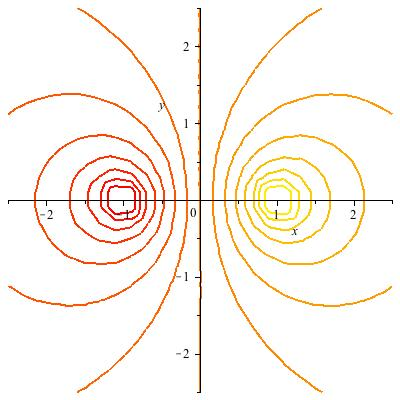
\includegraphics[width=2.2in]{VOLUMEN_1/05_Analisis_Vectorial/Figuras/Figura5_5.jpg}
\caption{Ejemplo de campo escalar $\phi=\phi\left( {\bf r}\right)$}
\label{FigCampoEscalar}
\end{minipage}
\end{figure}
%%%%%%%%%%%%%%%%%
\[
\phi\left( {\bf r}\right)  =\phi(x,y)  =\ln\left(  {\left(
x+1\right)^{2}}+{y}^{2}\right)  -\ln\left(  {\left(  x-1\right)^{2}
}+{y}^{2}\right)\,.
\]

La representaci�n de este campo escalar se puede apreciar en la figura \ref{FigCampoEscalar}.

\subsection{Campos escalares y superficies}
\label{CamposEscalares}
\index{Campos!Escalares}
\index{Escalares!Campos}
En la figura \ref{FigCampoTemperaturas} se ilustra el campo escalar  de temperaturas para la siguiente funci�n:
\[
T=T(x,y)  =70+180 {e}^{-(x-3)^2/10-(y-2)^2/10}\,.
\]
%%%%%%%%%%%%%%%%%
\begin{figure}[h]
\begin{minipage}{7.4cm}
Por lo tanto, por un campo escalar entenderemos a toda funci�n escalar de argumento vectorial, es decir, la funci�n que asociar� cada punto del espacio con un n�mero. Esto es: 
\[
\phi:\mathds{R}^{n}\rightarrow\mathds{R}
\]
\[
\phi=\phi\left({\bf r}\right) \quad \Rightarrow  \phi=\phi\left( x^{i}\right)  =\phi\left(  \tilde{x}^{i}\right)  \,.
\]

Estamos enfatizando el hecho que un campo escalar no variar� bajo cambios de las coordenadas en su argumento. Adicionalmente recalcamos que es indistinto hablar de vectores 
$\phi=\phi\left({\bf r}\right)$  o sus coordenadas $\phi=\phi\left( x^{i}\right)$. 

\end{minipage} \hfill 
\begin{minipage}{8.0cm} 
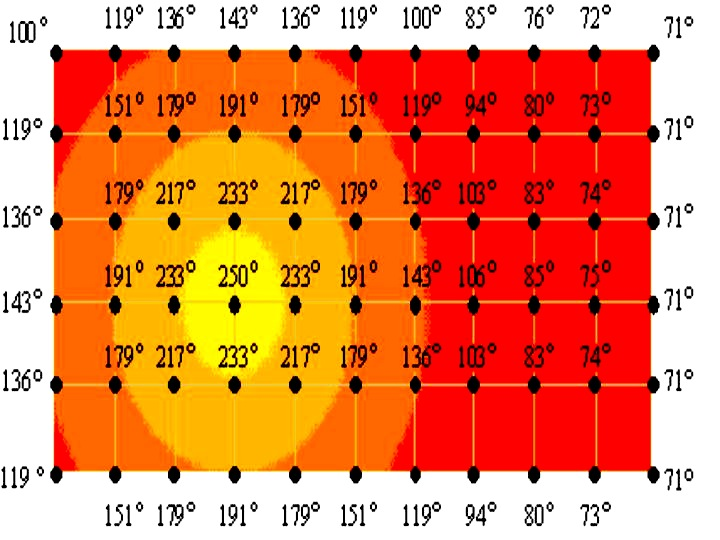
\includegraphics[width=2.5in]{VOLUMEN_1/05_Analisis_Vectorial/Figuras/Figura5_6.jpg}
\caption{Campo escalar  $T=T\left(x,y\right)$}
\label{FigCampoTemperaturas}
\end{minipage}
\end{figure}
%%%%%%%%%%%%%%%%%

En un mapa o diagrama de temperaturas, es posible unir los diferentes puntos con igual temperatura, y as� tendremos las curvas isotermas, tal y como se observa en la figura \ref{FigIsotermas}. 

Por otra parte, un campo escalar $\phi=\phi\left(  x^{1},x^{2}\right)$ definir� diferentes superficies si la representamos en $\mathds{R}^{3}$ de la forma: $x^{3}=\phi\left(x^{1},x^{2}\right)$.  De esta manera tendremos curvas de nivel o isocurvas las cuales se corresponden a las soluciones de $\phi=\phi\left(  x^{i}\right)= cte$.  Tal y como se ilustra en la figura \ref{FigCurvaNivel}, los diferentes planos  para $z= cte$,  cortan la superficie dada por la funci�n $z$ y definen las diferentes curvas de nivel 
$g\left(x,y\right)=k$.
%%%%%%%%%%%%%%%%%
\begin{figure}[h]
\begin{minipage}{7.4cm}
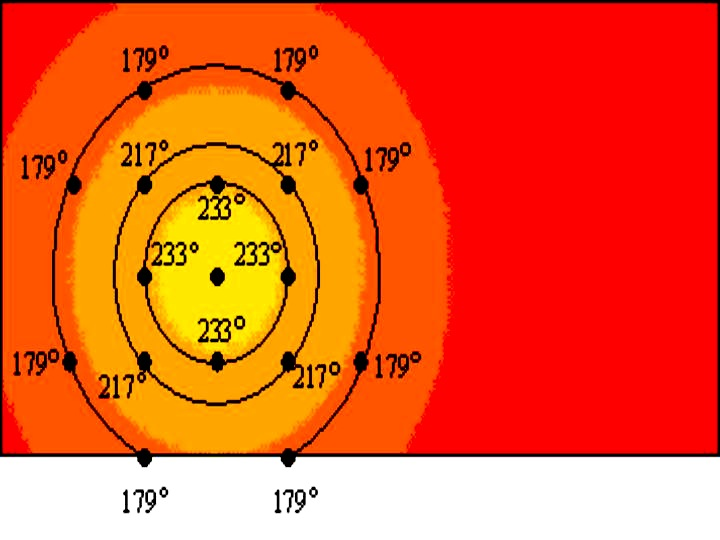
\includegraphics[width=2.4in]{VOLUMEN_1/05_Analisis_Vectorial/Figuras/Figura5_7.jpg}
\caption{Curvas Isotermas $T=T(x,y)=cte$.}
\label{FigIsotermas}
\end{minipage} \hfill 
\begin{minipage}{8.0cm} 
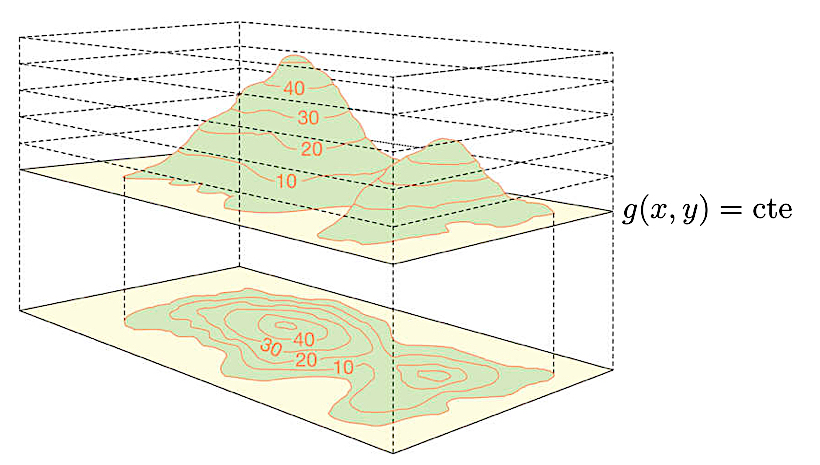
\includegraphics[width=2.4in]{VOLUMEN_1/05_Analisis_Vectorial/Figuras/Figura5_8.jpg}
\caption{Curvas de nivel para una funci�n $z=g\left(x,y\right)= cte$.}
\label{FigCurvaNivel}
\end{minipage}
\end{figure}
%%%%%%%%%%%%%%%%%

\subsection{Campos vectoriales y curvas integrales}
\label{CamposVectoriales}
\index{Campos!Vectoriales}
\index{Vectoriales!Campos}
Consideremos ahora un campo vectorial ${\bf A}\left({\bf r}\right)$ 
y estudiemos su representaci�n, y lo que es m�s importante, su variaci�n. Los campos vectoriales vienen a ser funciones vectoriales de varias variables en la que a cada punto del espacio o dominio se le asigna el vector, es decir: ${\bf A}\left({\bf r}\right):\mathds{R}^{n}\rightarrow\mathds{R}^n\,.$

Tal y como hemos dicho y volvemos a representar
en la figura \ref{FigCampoVectorial14}, los campos vectoriales asocian un vector (con su m�dulo direcci�n y sentido) a cada punto del espacio. Com�nmente, nos referimos a campos vectoriales seg�n el caso: \textit{campos de fuerza} (el vector del campo es una fuerza), \textit{campo de velocidades} (el vector del campo es una velocidad).

Del mismo modo, a aquellas l�neas a las cuales los vectores son tangentes se les dominan \textit{l�neas de campo, curvas integrales} o simplemente \textit{l�neas de flujo} o de \textit{corriente}. A las trayectorias ortogonales a estas l�neas, vale decir, a aquellas l�neas cuyos vectores tangentes son ortogonales al campo, se les denominar�n \textit{l�neas equipotenciales}.
\index{L�neas!de campo}
\index{L�neas!de flujo}
\index{Campo!Lineas de}
\index{Campo!de fuerza}
\index{Curvas!integrales}
\index{L�neas!Equipotenciales}
\index{Equipotenciales!L�neas}

El ejemplo m�s emblem�tico lo constituye el gradiente de un campo escalar ${\boldsymbol \nabla}\phi\left(x,y\right)$. Las \textit{l�neas equipotenciales} las define el campo
escalar mismo, $\phi(x,y)  =z= cte$ (curva de nivel) y construimos un campo vectorial con su gradiente, 
${\boldsymbol \nabla} \phi\left(x,y\right)$. 
Como el gradiente es perpendicular a la curva de nivel tendremos que las \textit{curvas integrales}, (l�neas de flujo o l�neas de corriente) del campo vectorial ${\boldsymbol \nabla}\phi(x,y)$ ser�n \textit{trayectorias ortogonales} a las \textit{curvas equipotenciales}.
\index{L�neas!de corriente}

Consideremos el caso bidimensional\footnote{El caso tridimensional s�lo a�ade complicaciones t�cnicas y no riqueza conceptual.} en coordenadas cartesianas, y tomemos el desplazamiento diferencial $\mathrm{d}{\bf r}$ en la direcci�n del campo vectorial 
${\bf A}$, es f�cil convencerse que:
\[
\mathrm{d}{\bf r}\varpropto {\bf A}(x,y)  =A_{x}\left(
x,y\right)  \mathbf{i}+A_{y}(x,y)  \mathbf{j}
\quad \Rightarrow  \frac{\mathrm{d}x}{A_{x}(x,y)}=
\frac{\mathrm{d}y}{A_{y}(x,y)  }\,,
\]
con lo cual encontramos las \textit{l�neas de flujo} o \textit{curvas
integrales} $y\left(x\right)$ del campo ${\bf A}\left(x,y\right) $
\[
\frac{\mathrm{d}y}{\mathrm{d}x}=\frac{A_{y}(x,y)  }{A_{x}\left(
x,y\right)  }\mathbf{\quad\Rightarrow\quad}y\left(  x\right)  =\int\frac
{A_{y}(x,y)  }{A_{x}(x,y)  }\mathrm{d}x\,.
\]

\begin{figure}[t]
\begin{center}
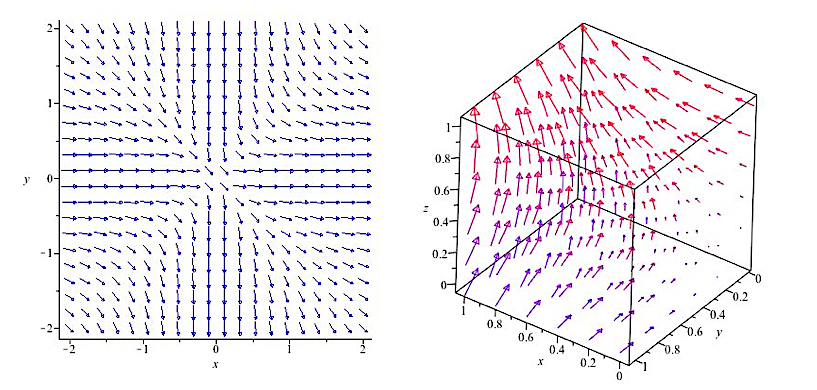
\includegraphics[height=2.4in,width=5.4in]
{VOLUMEN_1/05_Analisis_Vectorial/Figuras/Figura5_9.jpg}
\caption{Campos vectoriales}
\label{FigCampoVectorial14}
\end{center}
\end{figure}

Otra forma, equivalente de ver lo anterior es que si 
${\bf A}={\bf a}\left(  x(t),y(t),z(t) ,t\right)$, entonces:
\[
\mathrm{d}{\bf r}  \varpropto{\bf A}  \quad \Rightarrow 
\mathrm{d}{\bf r}\times {\bf A} =0\quad \Rightarrow 
\left|
\begin{array}
[c]{ccc}
\mathbf{i} & \mathbf{j} & \mathbf{k}\\
\mathrm{d}x & \mathrm{d}y & \mathrm{d}z\\
A_{x}  & 
A_{y} & 
A_{z}
\end{array}
\right| =0\,.
\]
Por lo cual $
\left[  A_{z}  \mathrm{d}y-A_{y}  \mathrm{d}z\right] \mathbf{i}+
\left[  A_{x}  \mathrm{d}z-A_{z}  \mathrm{d}x\right] \mathbf{j}+
\left[  A_{y}  \mathrm{d}x-A_{x}  \mathrm{d}y\right]\mathbf{k}=0\,,
$ 
para que finalmente
\[
\frac{\mathrm{d}x}{A_{x}\left(  x(t)  ,y(t)
,z(t)  ,t\right)  }=\frac{\mathrm{d}y}{A_{y}\left(  x\left(
t\right)  ,y(t)  ,z(t)  ,t\right)  }=\frac
{\mathrm{d}z}{A_{z}\left(  x(t)  ,y(t)  ,z\left(
t\right)  ,t\right)  }\,.
\]
La integral de estas ecuaciones definir�n las l�neas de flujo o
curvas integrales.

\subsubsection{Trayectorias ortogonales a las l�neas de flujo}
\label{TrayectoriasOrtogonales}
\index{Trayectorias!ortogonales}
Para encontrar las \textit{trayectorias ortogonales} al campo vectorial o las \textit{l�neas equipotenciales} construimos un campo vectorial ${\bf A}^{\bot}\left(x,y\right)$ 
que sea ortogonal en todo punto a ${\bf A}(x,y)  $
\[
{\bf A}^{\bot}(x,y)  \cdot{\bf A}(x,y) =0 \quad \Rightarrow  
A_{x}(x,y)  A_{x}^{\bot}\left(x,y\right) +
A_{y}(x,y)  A_{y}^{\bot}(x,y) =0\quad \Rightarrow  
\frac{A_{x}(x,y) }{A_{y}\left(x,y\right)  }=
-\frac{A_{y}^{\bot}\left(x,y\right)  }{A_{x}^{\bot}\left(x,y\right)}\,,
\]
donde ${\bf A}^{\bot}\left(x,y\right)=A_{x}^{\bot}\left(x,y\right)  \mathbf{i} +A_{y}^{\bot}\left(x,y\right)  \mathbf{j}\,,$ 
y ahora procedemos del mismo modo pero con el campo vectorial 
${\bf A}^{\bot}\left(x,y\right)$
\[
\frac{\mathrm{d}y}{\mathrm{d}x}=-\frac{A_{y}^{\bot}\left(x,y\right)  }
{A_{x}^{\bot}\left(x,y\right)  }\quad \Rightarrow  y\left(
x\right)  =-\int\frac{A_{y}^{\bot}\left(x,y\right)  }{A_{x}^{\bot}\left(
x,y\right)}\mathrm{d}x\,.
\]

\subsection{Flujo de campos vectoriales}
\label{FlujosVectoriales}
\index{Flujo!Campos Vectorial}
\index{Campo! vectorial, flujo de}
\index{Vectorial!Flujo de campo}
Podemos tambi�n imaginar flujo de campos vectoriales. Para ello, consideramos una superficie infinitesimal $\mathrm{d}{\bf S}=\left\| \mathrm{d}{\bf S}\right\|  \hat{\bf n}_{s}$, con $\hat{\bf n}_{s}$ el vector unitario normal esa superficie $S$. Entonces, la cantidad
\[
\mathrm{d}F={\bf A} \cdot \mathrm{d}{\bf S}={\bf A}\cdot\hat{\bf n}_{s}\ \mathrm{d}S \quad \Rightarrow  F=\iint_{s}{\bf A} \cdot \mathrm{d}{\bf S} = \iint_{s}{\bf A}\cdot\hat{\bf n}_{s}\ \mathrm{d}S  =
\iint_{s}A_{\hat{\bf n}}\ \mathrm{d}S\,,
\]
representar� el flujo diferencial del campo vectorial a trav�s de la superficie $\mathrm{d}{\bf S}$. Hemos denotado $A_{\hat{\bf n}}$ como la componente de ${\bf A}$ a lo largo de $\hat{\bf n}_{s}$. Hay que hacer notar que $F=\iint_{s}{\bf A}\cdot\mathrm{d}{\bf S}$, el flujo total, es un escalar independiente del sistema de coordenadas y que en coordenadas cartesianas puede expresarse como
\[
\mathrm{d}F={\bf A}\cdot\hat{\bf n}_{s}\ \mathrm{d}S=A^{1}\cos\left(
\widehat{\hat{\bf n}_{s}\ A^{1}}\right)  +A^{2}\cos\left(  \widehat{\hat{\bf n}
_{s}\ A^{2}}\right)  +A^{3}\cos\left(  \widehat{\hat{\bf n}_{s}\ A^{3}}\right)\,,
\]
donde $\left\{A^{1},A^{2},A^{3}\right\}$ son las componentes cartesianas del vector ${\bf A}$. El flujo ser� m�ximo cuando el campo es paralelo a $\mathrm{d}{\bf S}$ y, obviamente nulo cuando el campo es paralelo a $\mathrm{d}{\bf S}$.

La idea que esta cantidad representa un flujo puede tenerse si pensamos en un fluido incompresible que fluye con un campo de velocidades
${\bf v}={\bf v}\left( {\bf r}\right)$.  El volumen que atraviesa una
determinada superficie en un intervalo de tiempo $\mathrm{d}t$. As�, $\mathrm{d}S$ definir� la base de un tubo de fluido y tendr� como ``altura'' a $\left\|  {\bf v}\right\|\cos\left(\widehat{\hat{\bf n}
_{s}\ {\bf v}}\right)  \mathrm{d}t$, ya que la altura no tiene por qu� ser perpendicular a la base\footnote{De serlo, $\cos\left(\widehat{\hat{\bf n} \ {\bf v}}\right)=1$ porque la velocidad es paralela a la normal.}. Por lo tanto, la cantidad de fluido que atraviesa la superficie por unidad de tiempo viene dada por
\[
\mathrm{d}F=
\left(  \left\|  {\bf v}\right\|  \cos\left(  \widehat{\hat{\bf n}_{s}\ {\bf v}}\right)  \right)  \mathrm{d}S=  {\bf v}\cdot\hat{\bf n}_{s}\ \mathrm{d}S  =  {\bf v}\cdot\mathrm{d}{\bf S}\quad \Rightarrow  
F =\iint_{s}{\bf v}\cdot\mathrm{d}{\bf S}=
\iint_{s}{\bf v}\cdot\hat{\bf n}_{s}\ \mathrm{d}S=\iint_{s}v_{\hat{\bf n}}\ \mathrm{d}S\,.
\]

M�s adelante estudiaremos las t�cnicas para calcular el flujo de un campo vectorial a trav�s de una superficie cerrada que encierran un volumen $V$. 

\subsection{{\color{Fuchsia}Ejemplos}}

\begin{enumerate}
\item Dado el siguiente campo vectorial
\[
{\bf A}=-x\mathbf{i}+y\mathbf{j}\quad \Rightarrow 
\frac{\mathrm{d}y}{\mathrm{d}x}=-\frac{y}{x}\quad \Rightarrow 
\int\frac{\mathrm{d}y}{y}=-\int\frac{\mathrm{d}x}{x}+C\quad \Rightarrow 
y\left(  x\right)  =\frac{1}{x}C\,,
\]
esto es,  las hip�rbolas $yx=C$.

\item Las trayectorias ortogonales al campo del  ejemplo anterior son la siguientes curvas:

\[
{\bf A}=-x\mathbf{i}+y\mathbf{j}\quad \Rightarrow 
{\bf A}^{\bot}=y\mathbf{i}+x\mathbf{j}\quad \Rightarrow 
\frac{\mathrm{d}y}{\mathrm{d}x}=\frac{x}{y}\quad \Rightarrow 
y\left(  x\right)  = \sqrt{C^{2} + x^{2}}\,.
\]


\end{enumerate}

\newpage
\subsection{{\color{red}Practicando con Maxima}} 
En esta secci�n aprovecharemos  la ocasi�n para mostrar algunas opciones que tienen que ver con los comandos para graficar curvas de nivel. Es recomendable consultar el manual de {\bf Maxima} para tener acceso al resto de posibilidades. 

La funci�n {\bf contour plot}(funcion, xrange, yrange, options) muestra un gr�fico con curvas de nivel de la funci�n en el rect�ngulo xrange-yrange. Los argumentos para las opciones son los mismos que se usan en {\bf plot3d}, como por ejemplo, la opci�n {\it legend} con un valor {\it false}, para eliminar la leyenda. 


Dado el campo de temperaturas $ T=T\left( x,y\right)  =70+180 {e}^{-(x-3)^2/10-(y-2)^2/10}$, mostraremos en este m�dulo algunas de las posibilidades utilizando como herramienta adicional la librer�a {\bf draw}.

%%%%%% INPUT:
\begin{minipage}[t]{8ex}
{\color{red}\bf \begin{verbatim} (%i1) 
\end{verbatim}}
\end{minipage}
\begin{minipage}[t]{\textwidth}{\color{blue}
\begin{verbatim}
load(draw)$
\end{verbatim}}
\end{minipage}

Dado el siguiente campo escalar:

%%%%%% INPUT:
\begin{minipage}[t]{8ex}
{\color{red}\bf \begin{verbatim} (%i2) 
\end{verbatim}}
\end{minipage}
\begin{minipage}[t]{\textwidth}{\color{blue}
\begin{verbatim}
T(x,y):=70+180*exp(-(x-3)^2/10-(y-2)^2/10);
\end{verbatim}}
\end{minipage}

%%% OUTPUT:
\begin{math}\displaystyle \parbox{8ex}{\color{labelcolor}(\%o2) }
 T(x,y):=70+180 {\tt exp}\left(-\frac{\left(x-3\right)^2}{10}-\frac{\left(y-2\right)^2}{10}\right)
\end{math}

El gr�fico m�s simple que podemos realizar es el siguiente

%%%%%% INPUT:
\begin{minipage}[t]{8ex}
{\color{red}\bf \begin{verbatim} (%i3) 
\end{verbatim}}
\end{minipage}
\begin{minipage}[t]{\textwidth}{\color{blue}
\begin{verbatim}
wxcontour_plot(T(x,y),[x,-2,10],[y,-4,10],[legend,false]);
\end{verbatim}}
\end{minipage}

%%% OUTPUT:
\begin{math}\displaystyle \parbox{8ex}{\color{labelcolor}(\%o3) }
\end{math}
\begin{figure}[h]
\begin{center}
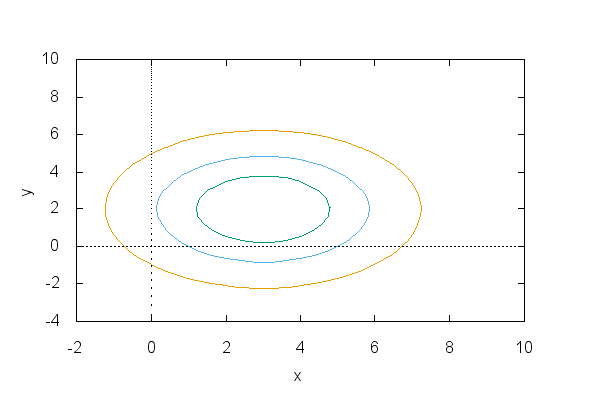
\includegraphics[height=2.6in,width=4.2in]{VOLUMEN_1/05_Analisis_Vectorial/Figuras/Figura5_9a.jpg}
\end{center}
\end{figure}

\newpage
Otra perspectiva es 

%%%%%% INPUT:
\begin{minipage}[t]{8ex}
{\color{red}\bf \begin{verbatim} (%i4) 
\end{verbatim}}
\end{minipage}
\begin{minipage}[t]{\textwidth}{\color{blue}
\begin{verbatim}
wxplot3d(T(x,y),[x,-2,10],[y,-4,10],[gnuplot_preamble,"set contour"]);
\end{verbatim}}
\end{minipage}

%%% OUTPUT:
\begin{math}\displaystyle \parbox{8ex}{\color{labelcolor}(\%o4) }
\end{math}

\begin{figure}[h]\nonumber
\begin{center}
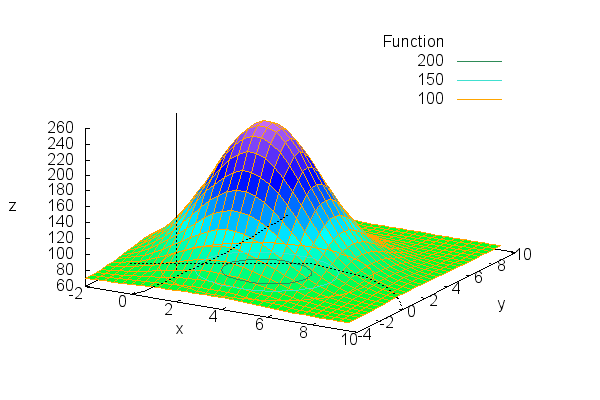
\includegraphics[height=2.6in,width=4.2in]{VOLUMEN_1/05_Analisis_Vectorial/Figuras/Figura5_9b.jpg}
\end{center}
\end{figure}


%%%%%% INPUT:
\begin{minipage}[t]{8ex}
{\color{red}\bf \begin{verbatim} (%i5) 
\end{verbatim}}
\end{minipage}
\begin{minipage}[t]{\textwidth}{\color{blue}
\begin{verbatim}
wxplot3d(T(x,y),[x,-2,10],[y,-4,10],[gnuplot_preamble,"set pm3d at b"]);
\end{verbatim}}
\end{minipage}

%%% OUTPUT:
\begin{math}\displaystyle \parbox{8ex}{\color{labelcolor}(\%o5) }
\end{math}

\begin{figure}[h]\nonumber
\begin{center}
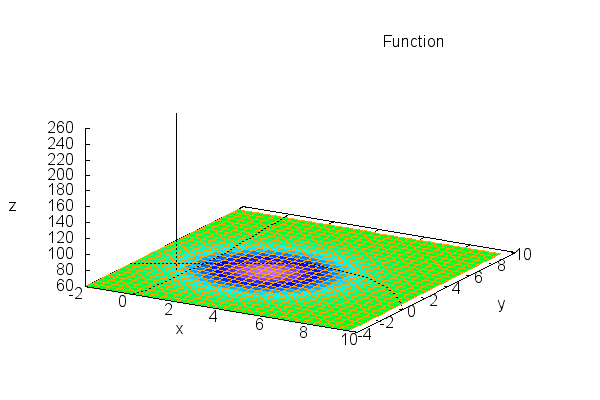
\includegraphics[height=2.6in,width=4.2in]{VOLUMEN_1/05_Analisis_Vectorial/Figuras/Figura5_9c.jpg}
\end{center}
\end{figure}

\newpage
%%%%%% INPUT:
\begin{minipage}[t]{8ex}
{\color{red}\bf \begin{verbatim} (%i6) 
\end{verbatim}}
\end{minipage}
\begin{minipage}[t]{\textwidth}{\color{blue}
\begin{verbatim}
wxdraw3d(enhanced3d=true,explicit(T(x,y),x,-2,10,y,-4,10),
contour_levels=8,contour=surface);
\end{verbatim}}
\end{minipage}

%%% OUTPUT:
\begin{math}\displaystyle \parbox{8ex}{\color{labelcolor}(\%o6) }
\end{math}

\begin{figure}[h]\nonumber
\begin{center}
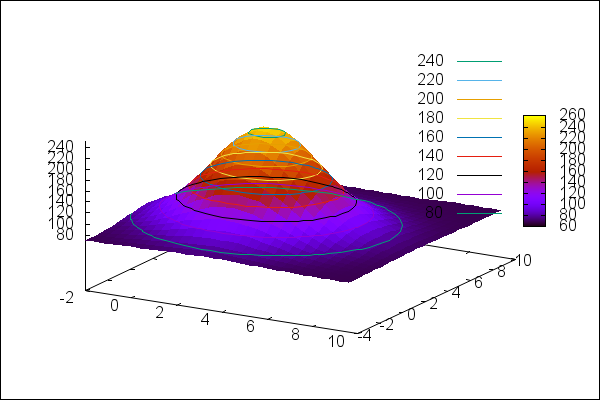
\includegraphics[height=2.6in,width=4.2in]{VOLUMEN_1/05_Analisis_Vectorial/Figuras/Figura5_9d.jpg}
\end{center}
\end{figure}

%\newpage

%%%%%% INPUT:
\begin{minipage}[t]{8ex}
{\color{red}\bf \begin{verbatim} (%i7) 
\end{verbatim}}
\end{minipage}
\begin{minipage}[t]{\textwidth}{\color{blue}
\begin{verbatim}
wxdraw3d(enhanced3d=true,explicit(T(x,y),x,-2,10,y, -4,10),
contour_levels=8,contour=map);
\end{verbatim}}
\end{minipage}

%%% OUTPUT:
\begin{math}\displaystyle \parbox{8ex}{\color{labelcolor}(\%o7) }
\end{math}

\begin{figure}[h!]\nonumber
\begin{center}
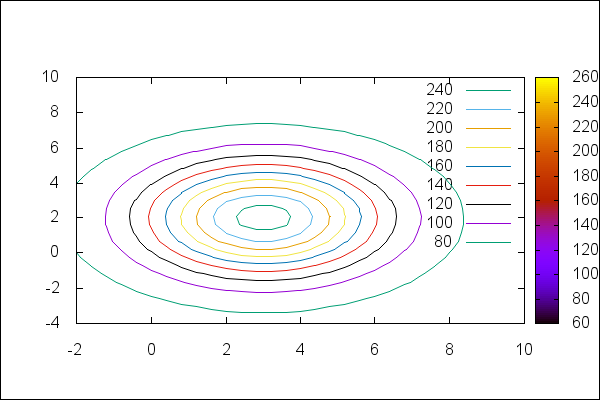
\includegraphics[height=2.5in,width=4.2in]{VOLUMEN_1/05_Analisis_Vectorial/Figuras/Figura5_9e.jpg}
\end{center}
\end{figure}


\begin{center}
{\color{red}\rule{15.8cm}{0.4mm}}
\end{center}


\subsection{{\color{OliveGreen}Ejercicios}}
\begin{enumerate}
\item Encuentre las curvas integrales y las trayectorias  ortogonales de los siguientes campos vectoriales
\begin{enumerate}
\item ${\bf F}(x,y) = -\frac{x}{2}{\bf i} - \frac{y}{2}{\bf j}$,
\item ${\bf F}(x,y) = xy{\bf i} +2x{\bf j}$,
\item ${\bf F}(x,y) = x^2{\bf i} -y{\bf j}$.
\end{enumerate}


\item El vector �rea para una superficie $S$ se define como  ${\bf S}=\iint_{s} \mathrm{d}{\bf S}\,,$ encuentre el vector �rea de la superficie: $x^2 + y^2 + z^2 = a^2$ con $z \leq 0$. Utilice el hecho de que en coordenadas esf�ricas 
$\mathrm{d}{\bf S} = a^2 \mathrm{sen}(\theta) \mathrm{d}\theta \mathrm{d}\varphi \ {\bf{\hat e}}_r$.
\end{enumerate}


\section{La fauna de los operadores vectoriales}
\label{faunadeoperadoresvectoriales}
\index{Operador!Vectorial}
\index{Vectorial!Operador}
A partir del concepto de campo escalar, presentaremos ahora una variedad de objetos diferenciales en el espacio tridimensional. Salvo que se diga lo contrario, utilizaremos el sistema de coordenadas cartesianas, que discutimos en la secci�n \ref{CoordenadasCartesianas} en la p�gina \pageref{CoordenadasCartesianas}. 

\subsection{Derivada direccional, diferencial total y gradiente}
\label{DerivadaDireccional}
\index{Derivada!Direccional}

\subsubsection{Derivada direccional de campos escalares}
\label{DerivDirEscalar}
\index{Campo!Escalar, derivada direccional}
\index{Derivada!Direccional, Campo escalar}
Para analizar los cambios en los campos escalares requerimos comparar dos ``instantes de tiempo'', para ello, parametrizamos las componentes del vector: $z  =\phi\left({\bf r}(t)  \right)  =g\left(  x(t)  ,y(t)  \right) \,,$ 
por lo tanto:
\[
\frac{\mathrm{d }\phi\left(  x(t)  ,y(t)  \right)}{\mathrm{d }t} =
\frac{\partial \phi\left(  x(t),y(t)  \right)  }{\partial x}\frac{\mathrm{d }x(t)}{\mathrm{d}t}+
\frac{\partial\phi\left(  x(t),y(t)  \right)  }{\partial y}\frac{\mathrm{d }y(t)}{\mathrm{d }t}=
{\boldsymbol \nabla} \phi\left(  x(t)  ,y(t)  \right)  \cdot \frac{\mathrm{d }{\bf r}(t)}{\mathrm{d }t}\,;
\]
donde hemos representado
\[
{\boldsymbol \nabla}\phi\left(x(t),y(t)  \right) = \frac{\partial\phi\left(x,y\right)}{\partial x}\mathbf{i}+
\frac{\partial\phi\left(x,y\right)}{\partial y}\mathbf{j} \qquad \mbox{y} \qquad  \frac{\mathrm{d}{\bf r}(t)}{\mathrm{d}t} = \frac{\mathrm{d}x(t)}{\mathrm{d}t} \mathbf{i} + \frac{\mathrm{d}y(t)}{\mathrm{d}t} \mathbf{j} \,.
\]

A ${\boldsymbol \nabla}\phi\left(x^i(t) \right)$  lo llamaremos el {\it gradiente} del campo escalar 
$\phi\left(x^i(t) \right)$, y tambi�n son muy comunes otras notaciones para el gradiente:
\[
{\boldsymbol \nabla}\phi\left(x(t),y(t) \right)=
\phi_{x}\left(x,y\right)  \mathbf{i}+\phi_{y}(x,y)\mathbf{j}=
\partial^{i}\phi\left(x,y\right) \mathbf{i}_i =
\phi^{,i}\left(x,y\right)\mathbf{i}_i\,,
\]

El gradiente de un campo escalar es uno de los objetos m�s �tiles del c�lculo vectorial,  el cual lo hemos utilizado de manera operacional y no nos hemos detenido a reflexionar sobre sus propiedades.

Es claro que cuando se tienen curvas de nivel $g\left(x,y\right)=z=\phi\left({\bf r}(t)  \right)=k=cte\,,$ obtenemos
\[
\frac{\mathrm{d}\phi\left(x(t),y(t)  \right)  }
{\mathrm{d }t}=\frac{\mathrm{d }k}{\mathrm{d }t}=0 
\quad \Rightarrow 
\frac{\mathrm{d}\phi\left(  x(t)  ,y(t)  \right)}{\mathrm{d}t}=0={\boldsymbol \nabla}\phi\left(  x(t)  ,y(t)\right)\cdot\frac{\mathrm{d }{\bf r}(t)}{\mathrm{d}t}\,,
\]
con lo cual, dado que $\frac{\mathrm{d}{\bf r}(t)}{\mathrm{d}t}$ es la tangente a la curva, entonces, el gradiente es perpendicular a la curva, tal y como se muestra en la figura \ref{FigMaxVariacion}. 

%%%%%%%%%%%%%%%%%
\begin{figure}[h]
\begin{center}
\includegraphics[width=3.5in]{VOLUMEN_1/05_Analisis_Vectorial/Figuras/Figura5_10.jpg}
\caption{Derivada direccional}
\label{Capt5AnalisisVectorial/FigDerivadaDireccional}
\label{FigDerivadaDireccional}
\end{center}
\end{figure}
%%%%%%%%%%%%%%%%%

Si se da el caso que la funci�n dependa de manera expl�cita del par�metro $t$, $\phi=\phi\left(x^i(t), t\right)$ tendremos que
\[
\phi=\phi\left(x(t), y(t), z(t), t\right)\quad \Rightarrow  
\frac{\mathrm{d}\phi}{\mathrm{d }t}=
\frac{\partial\phi\left(  x^i(t),t\right)}{\partial t}=
{\boldsymbol \nabla} \phi\left( x^i(t) ,t\right)
\cdot\frac{\mathrm{d }{\bf r}(t)  }{\mathrm{d }t}\,,
\]y, en el caso particular en que el par�metro es la longitud de arco $s$ a lo largo de la curva, la derivada total de $\phi$ con respecto a $s$ a lo largo de la curva vendr� dada por
\begin{equation}
\label{DerivadaTotal}
\frac{\mathrm{d }\phi}{\mathrm{d}s}=
{\boldsymbol \nabla} \phi\left(x^i(t), t\right) \cdot { \boldsymbol {\hat \tau}}\,,
\end{equation}
donde ${ \boldsymbol {\hat \tau}}$ es el vector unitario tangente a la curva en el punto dado. Adem�s, cuando  $\phi\left(x^i(t), t\right)=k$, entonces, al ser ${ \boldsymbol {\hat \tau}}$ tangente a esta superficie en alg�n punto, es claro que ${\mathrm{d}\phi}/{\mathrm{d}s}=0$ en esa direcci�n y ${\boldsymbol \nabla} \phi \cdot { \boldsymbol {\hat \tau}} =0$. Por lo tanto, ${\boldsymbol \nabla} \phi$ ser� normal a la superficie $\phi\left(x^i(t), t\right)=k$.


Por otro lado, la derivada direccional indicar� la tasa de cambio del campo escalar en la direcci�n que apuntemos. Es una generalizaci�n de la idea que surge de parametrizar la curva o de la derivada total respecto al tiempo.
Dados dos puntos $M$ y $M^{\prime}$ definiremos la derivada en la direcci�n de un vector unitario $\hat{\bf u}\leftrightarrow\overrightarrow{M^{\prime}M}$ como se muestra a continuaci�n:
\begin{equation}
\label{EqDerivadaDireccional}
\mathbb{D}_{\hat{\bf u} }\phi \equiv \lim_{M^{\prime}\rightarrow M}\frac{\phi\left(  M^{\prime}\right)
-\phi\left(  M\right)  }{\left|  \overrightarrow{M^{\prime}M}\right|  }= \frac{\mathrm{d }\phi}{\mathrm{d }\lambda} =
{\boldsymbol \nabla} \phi\left(x,y\right)  \cdot \hat{\bf u} \,.
\end{equation}

Tal y como se puede apreciar en la figura \ref{FigDerivadaDireccional} la derivada direccional est� representada por la pendiente de la recta tangente a la curva que surge como intersecci�n entre la superficie $\phi\left(x,y\right)=z=k=cte$,  el plano vertical formado por el eje $z$ y el vector unitario $\hat{\bf u}$. 


En este punto, varias reflexiones se pueden derivar del concepto de derivada total. 
\begin{itemize}
  \item La primera es que dado que,  la derivada direccional a lo largo de $\hat{\bf u}$ es
\[
  \mathbb{D}_{ \hat{\bf u} }\phi   =
{\boldsymbol \nabla} \phi  \cdot\hat{\bf u}   =
\left|  {\boldsymbol \nabla}\phi  \right| \cos\widehat{\left( {\boldsymbol \nabla} \phi  ,\hat{\bf u}\right) }\,,
\]
(donde hemos denotado por $\widehat{{\boldsymbol \nabla}\phi ,\hat{\bf u}}$ como el �ngulo que forman los vectores ${\boldsymbol \nabla}\phi$ y $\hat{\bf u})$, el valor m�ximo de la derivada direccional ser�
\[
  \mathbb{D}_{ \hat{\bf u}}\phi_{\max}=
\left| {\boldsymbol \nabla}\phi  \right| =
\sqrt{\partial^{i}\phi\partial_{i}\phi}\equiv\sqrt{\frac{\partial\phi}{\partial x_{i}} \frac{\partial\phi}{\partial x^{i}}}\equiv\sqrt{\left(  \frac{\partial\phi}{\partial x^{1}}\right)^{2}+\left(  \frac{\partial\phi}{\partial x^{2}}\right)^{2} +\left(  \frac{\partial\phi}{\partial x^{3}}\right)^{2}}\,.
\]
Es decir, cuando $\hat{\bf u}$ apunta en la direcci�n del gradiente o, lo que es lo mismo, en la direcci�n de la mayor tasa de cambio; el valor m�ximo lo indica la direcci�n del gradiente. O dicho de otro modo, en un determinado punto $M$ de las superficie $\phi\left(x,y\right)  =z$ el vector ${\boldsymbol \nabla}\phi$
apunta en la direcci�n de la m�xima tasa de cambio, tal y como podemos apreciar en la figura \ref{FigMaxVariacion}.
  \item La segunda reflexi�n es dado que el gradiente es ortogonal a la superficie, los vectores perpendiculares a �l conformar�n el plano tangente a la superficie en un determinado punto.
  %%%%%% Voy por aqu�
  \item La tercera emerge de la misma definici�n (\ref{EqDerivadaDireccional}), es claro que la derivada direccional es un escalar, por lo tanto, como $\hat{\bf u}$ es un vector,  ${\boldsymbol \nabla} \phi\left(x,y\right)$ debe ser una $1-$forma. Vale decir, como veremos con mas detalle en las secciones  \ref{GradCoordCurv} y \ref{DivergFlujoVectorial}
\[
\mbox{grad}\ \phi= {\boldsymbol \nabla}\phi=
\frac{1}{h_{1}}\frac{\partial \phi}{\partial q^{1}}\left<\mathrm{e}^{1}\right| +
\frac{1}{h_{2}}\frac{\partial \phi}{\partial q^{2}}\left<\mathrm{e}^{2}\right| +
\frac{1}{h_{3}}\frac{\partial \phi}{\partial q^{3}}\left<\mathrm{e}^{3}\right|= 
\frac{\left<\mathrm{e}^{i}\right|}{h_{\tilde i}} \frac{\partial \phi}{\partial q^{i}} = \frac{\left<\mathrm{e}^{i}\right|}{h_{\tilde i}} \partial_i \phi \,.
\] Donde denotamos $h_{\tilde i}=\left\| \frac{\partial \left< r \right|  }{\partial q^{i}}\right\|  =\sqrt{g_{ii}}$ los factores de  escala que acompa�a a la base $\left<\mathrm{e}^{i}\right|$ generalizada.
\end{itemize}


\begin{figure}[t]
\begin{center}
\includegraphics[height=2.5in,width=5.5in]
{VOLUMEN_1/05_Analisis_Vectorial/Figuras/Figura5_11.jpg}
\caption{Direcci�n de m�xima variaci�n en una funci�n.  Gradiante y tangente de una funci�n.}
\label{FigMaxVariacion}
\end{center}
\end{figure}

\subsubsection{Gradiente y flujo de un campo vectorial}

Podemos utilizar la idea de flujo de un campo vectorial y generalizar la definici�n de gradiente para que sea independiente de las coordenadas.
\[
{\boldsymbol \nabla}\phi=\mbox{grad}\ \phi=\lim_{V\rightarrow0}
\frac{1}{V}\iint_{s}\phi(x,y,z)  \mathrm{d}{\bf S}=\lim
_{V\rightarrow0}\frac{1}{V}\iint_{s}\phi(x,y,z)  \ \hat{\bf n}
_{s}\ \mathrm{d}S\,.
\]
Supongamos que construimos un campo vectorial de la forma siguiente
\[
{\bf a}\left(x,y,z\right)  ={\bf c}\ \phi\left(  x,y,z\right)\,, \quad \text{con }{\bf c}=cte\,,
\]
con lo cual
\[
F=\iint_{s}{\bf c}\ \phi(x,y,z)  \cdot\mathrm{d}{\bf S}=\iint_{s}{\bf c}\ \phi(x,y,z)  \cdot\hat{\bf n}_{s}\ \mathrm{d}S\,.
\]

Es claro que esta expresi�n vale para todos los sistemas de coordenadas. En particular, para un sistema de coordenadas cartesianas construimos un cubo diferencial con aristas que coincidan con los ejes coordenados. Entonces se
tiene que las caras del cubo ser�n
\[
\mathrm{d}{\bf S}_{x+} =\left(\mathrm{d}y\ \mathrm{d}z\right)\mathbf{i}\,;\quad
\mathrm{d}{\bf S}_{x-}=-\left(\mathrm{d}y\ \mathrm{d}z\right)  \mathbf{i}\,; \quad 
\mathrm{d}{\bf S}_{y+}=\left(\mathrm{d}x\ \mathrm{d}z\right)\mathbf{j}\,;\quad
\mathrm{d}{\bf S}_{y-}=-\left(\mathrm{d}x\ \mathrm{d}z\right) \mathbf{j}\,; 
\]
\[
\mathrm{d}{\bf S}_{z+} =\left(\mathrm{d}x\ \mathrm{d}y\right)\mathbf{k}\,;\quad
\mathrm{d}{\bf S}_{z-}=-\left(\mathrm{d}x\ \mathrm{d}y\right)\mathbf{k}\,,
\label{caras}
\]
con lo cual, el flujo por las seis caras es
\begin{eqnarray*}
\mathrm{d}F&=&{\bf c}\ \phi(x,y,z)  \cdot\mathrm{d}{\bf S}_{x+}+
{\bf c}\ \phi(x,y,z)  \cdot\mathrm{d}{\bf S}_{x-}+ {\bf c}\ \phi(x,y,z)  \cdot\mathrm{d} {\bf S}_{y+} \\
&+&{\bf c}\ \phi(x,y,z)  \cdot\mathrm{d}{\bf S}_{y-}+{\bf c}\ \phi(x,y,z) \cdot\mathrm{d}{\bf S}_{z+}+{\bf c}\ \phi\left(x,y,z\right)  \cdot\mathrm{d}{\bf S}_{z-} \,,
\end{eqnarray*}
por lo tanto
\begin{eqnarray*}
\mathrm{d}F&=&{\bf c} \left[  \phi\left(  x+\mathrm{d}x,y,z\right)  
\mathrm{d}y\ \mathrm{d}z-\phi(x,y,z)  \mathrm{d}y\ \mathrm{d}z+\phi\left(x,y+\mathrm{d}y,z\right)  \mathrm{d}x\ \mathrm{d}z-\phi\left(  x,y,z\right)
\mathrm{d}x\ \mathrm{d}z\right.\\
&+&\left.\phi\left(x,y,z+\mathrm{d}z\right)  \mathrm{d}x\ \mathrm{d}y-\phi(x,y,z)  \mathrm{d}x\ \mathrm{d}y\right]\\
&=&{\bf c}\left[ \left\{  \phi\left(  x+\mathrm{d}x,y,z\right)  -\phi\left(
x,y,z\right)  \right\}  \mathrm{d}y\ \mathrm{d}z+\left\{  \phi\left(x,y+\mathrm{d}y,z\right)  -\phi(x,y,z)  \right\}  \mathrm{d}x\ \mathrm{d}z+\right. \\
&+& \left. \left\{  \phi\left(  x,y,z+\mathrm{d}z\right)  -\phi\left(
x,y,z\right)  \right\}  \mathrm{d}x\ \mathrm{d}y\right]\,.
\end{eqnarray*}

Como estamos considerando un ``cubo diferencial'' podemos desarrollar por Taylor hasta primer orden, por lo que:
\[
\phi\left(x+\mathrm{d}x,y,z\right)   \approx\phi\left(x,y,z\right)
+\frac{\partial \phi\left(x,y,z\right)}{\partial x}\mathrm{d}x\,,\quad
\phi\left(x,y+\mathrm{d}y,z\right)   \approx\phi\left(x,y,z\right)
+\frac{\partial \phi\left(x,y,z\right)}{\partial y}\mathrm{d}y\,,
\]
\[
\phi\left(x,y,z+\mathrm{d}z\right)   \approx\phi\left(x,y,z\right)
+\frac{\partial \phi\left(  x,y,z\right)}{\partial z}\mathrm{d}z\,.
\]
Con lo cual
\begin{eqnarray*}
\mathrm{d}F &=&\frac{\partial \phi(x,y,z)  }{\partial x}
\mathrm{d}x\ \mathrm{d}y\ \mathrm{d}z+\frac{\partial \phi\left(
x,y,z\right)  }{\partial y}\mathrm{d}y\ \mathrm{d}x\ \mathrm{d}z+\frac
{\partial \phi(x,y,z)  }{\partial z}\mathrm{d}z\ \mathrm{d}
x\ \mathrm{d}y\\
&=&\left(  \frac{\partial \phi\left(x,y,z\right)  }{\partial
x}+\frac{\partial \phi\left(x,y,z\right)  }{\partial y}+\frac
{\partial \phi\left(x,y,z\right)  }{\partial z}\right)  \mathrm{d}V
\quad \Rightarrow  {d}F=\mbox{grad}\ \phi\ \mathrm{d}V\,,
\end{eqnarray*}
entonces
\[
{\bf \mbox{grad}}\ \phi =\frac{\mathrm{d}F}{\mathrm{d}V}=
\lim_{\Delta V \rightarrow0} \frac{F_{2}-F_{1}}{V_{2}-V_{1}}=
\lim_{V\rightarrow0}\frac{1}{V}\iint_{s}\phi\left(x,y,z\right)  \mathrm{d}{\bf S}=
\lim_{V\rightarrow0}\frac{1}{V}\iint_{s}\phi\left(x,y,z\right)  \ \hat{\bf n}\ \mathrm{d}S\,.
\]

N�tese que hemos supuesto que $\Delta V\equiv V_{2}\equiv V$ y que $F_{2}=\iint_{s}\phi(x,y,z)  \mathrm{d}{\bf S}$. Que quiere decir que tanto $V_{1}\sim0$ con lo cual el flujo a trav�s de un punto se anula, $F_{1}\sim0$.

\subsubsection{Gradiente y coordenadas curvil�neas}
\label{GradCoordCurv}
\index{Gradiente!Coordenadas generalizadas}
\index{Coordenadas Generalizadas!Gradiente}
La generalizaci�n de la expresi�n del gradiente en coordenadas curvil�neas es inmediata a partir de diferencial total de una funci�n $\phi(q^{1},q^{2},q^{3})$. Esto es
\[
\phi(q^{1},q^{2},q^{3}) =\phi\left(  q^{j}\right) \quad \Rightarrow  \mathrm{d }\phi=\frac{\partial \phi(q^{1},q^{2},q^{3})} {\partial q^{j}}\mathrm{d} q^{j}
\]
con
\[
\mbox{grad}\ \phi \left(q^{i}\right)   =  
\frac{1}{\left\|  \frac{\partial \left< {r}\right|  }{\partial q^{1}}\right\|}\frac{\partial \phi}{\partial q^{1}}
\left<\mathrm{e}^{1}\right| +
\frac{1}{\left\|  \frac{\partial \left< {r}\right|}{\partial q^{2}}\right\|}\frac{\partial \phi}{\partial q^{2}}
\left<\mathrm{e}^{2}\right| +
\frac{1}{\left\|  \frac{\partial \left< {r}\right| }{\partial q^{3}}\right\|}\frac{\partial \phi}{\partial q^{3}}
\left<\mathrm{e}^{3}\right|\,,
\]
y
\[
\left<\mathrm{d}{r}\right| = \frac{\partial \left< {r}\right| }{\partial q^{1}}\mathrm{d}q^{1}+
\frac{\partial \left< {r}\right|}{\partial q^{2}}\mathrm{d}q^{2}
+\frac{\partial \left< {r}\right|}{\partial q^{3}}\mathrm{d}q^{3} \equiv 
\left\|  \frac{\partial \left< {r}\right| }{\partial q^{1}} \right\|  \left<\mathrm{e}^{1}\right|\ \mathrm{d}q^{1}
+\left\|  \frac{\partial \left< {r}\right| }{\partial q^{2}}\right\|  \left<\mathrm{e}^{2}\right|\ \mathrm{d}q^{2}
+\left\|  \frac{\partial \left< {r}\right| }{\partial q^{3}}\right\|  \left<\mathrm{e}^{3}\right| \ \mathrm{d}q^{3}\,,
\]
ya que, al igual que en el caso de los vectores, la base del espacio dual se construye como
\[
\left<\mathrm{e}^{1}\right| =\frac{1}{\left\|  \frac{\partial \left< {r}\right| }{\partial q^{1}}\right\|  }
\frac{\partial \left< {r}\right| }{\partial q^{1}}; \quad 
\left<\mathrm{e}^{2}\right| =\frac{1}{\left\| \frac{\partial \left< {r}\right| }{\partial q^{2}}\right\|
}\frac{\partial \left< r\right| }{\partial q^{2}}; \quad \mathrm{y} \quad
\left<\mathrm{e}^{3}\right| =\frac{1}{\left\| \frac{\partial \left< {r}\right| }{\partial q^{3}}\right\|
}\frac{\partial \left< {r}\right| }{\partial q^{3}}\,.
\]

Es decir, la forma general del gradiente para un sistema de coordenadas curvil�neas ortogonales es
\[
\mbox{grad}\ \phi= {\boldsymbol \nabla}\phi=
\frac{1}{h_{1}}\frac{\partial \phi}{\partial q^{1}}\left<\mathrm{e}^{1}\right| +
\frac{1}{h_{2}}\frac{\partial \phi}{\partial q^{2}}\left<\mathrm{e}^{2}\right| +
\frac{1}{h_{3}}\frac{\partial \phi}{\partial q^{3}}\left<\mathrm{e}^{3}\right|= 
\frac{\left<\mathrm{e}^{i}\right|}{h_{\tilde i}} \frac{\partial \phi}{\partial q^{i}} = \frac{\left<\mathrm{e}^{i}\right|}{h_{\tilde i}} \partial_i \phi \,.
\label{gradphi}
\]
Donde denotamos $h_{\tilde i}=\left\| \frac{\partial \left< r \right|  }{\partial q^{i}}\right\|  =\sqrt{g_{ii}}$ el factor de escala
que acompa�a a la base $\left\{\left<\mathrm{e}^{i}\right|\right\}$ y {\bf debe quedar claro} que en el lado derecho de la ecuaci�n (\ref{gradphi}) la suma es �nicamente sobre los �ndices de $\left|  {\mathrm{e}}_{i}\right>$ y $\partial_i $. La tilde en el indice ${\tilde i}$ es para indicar que simplemente replica el valor que toma el �ndice $i$.




\subsection{Divergencia y flujo en campos vectoriales}
\label{DivergFlujoVectorial}
\index{Divergencia}
\index{Flujo!Campos vectoriales}
Revisando con un poco m�s de cuidado la expresi�n para el gradiente podemos ver que 
\[
\mbox{grad} \ \phi=
\left( \frac{\left< \mathrm{e}_{1}\right| }{h_{1}}\frac{\partial}{\partial q^{1}}+
\frac{\left< \mathrm{e}_{2}\right|}{h_{2}}\frac{\partial}{\partial q^{2}}+
\frac{\left< \mathrm{e}_{3}\right|}{h_{3}}\frac{\partial}{\partial q^{3}}\right) \phi\,,
\]
es decir, con esta inspiraci�n podemos construir un funcional lineal 
\[
{\boldsymbol \nabla} \equiv  
\frac{\left< \mathrm{e}_{1}\right|}{\mathcal{H}}\frac{\partial}{\partial q^{1}}+
\frac{\left< \mathrm{e}_{2}\right|}{\mathcal{F}}
\frac{\partial}{\partial q^{2}}+
\frac{\left< \mathrm{e}_{3}\right|}{\mathcal{G}}\frac{\partial}{\partial q^{3}}\,,
\]
donde: $\mathcal{H}=\mathcal{H}(h_{1},h_{2},h_{3})$, $\mathcal{F}=\mathcal{F}(h_{1},h_{2},h_{3})$ y $\mathcal{G}=\mathcal{G}(h_{1},h_{2},h_{3})$. 

Con lo cual, si cuidamos el orden de operaci�n, podremos realizar un ``producto interno entre una 1-forma, ${\boldsymbol \nabla}$ y un vector ${\bf a}$'' de la forma 
\begin{eqnarray*}
{\boldsymbol \nabla} \cdot {\bf a} &\equiv&
\left[
\frac{\left< \mathrm{e}_{1}\right|}{\mathcal{H}}\frac{\partial}{\partial q^{1}}+
\frac{\left< \mathrm{e}_{2}\right|}{\mathcal{F}}\frac{\partial}{\partial q^{2}}+
\frac{\left< \mathrm{e}_{3}\right|}{\mathcal{G}}\frac{\partial}{\partial q^{3}}
\right] \cdot 
\left[a^{1}\left| \mathrm{e}_{1}\right> + a^{2}\left|\mathrm{e}_{2}\right>+a^{2}\left|  \mathrm{e}_{3}\right> \right] \\
&=&
\frac{\left< \mathrm{e}_{1}\right|}{\mathcal{H}}\cdot
\frac{\partial\left[a^{1}\left|\mathrm{e}_{1}\right>+a^{2}\left|\mathrm{e}_{2}\right> +a^{2}\left|\mathrm{e}_{3}\right> \right]}{\partial q^{1}} +
\frac{\left< \mathrm{e}_{2}\right|  }{\mathcal{F}}\cdot
\frac{\partial\left[a^{1}\left|\mathrm{e}_{1}\right> +a^{2}\left|  \mathrm{e}_{2}\right> +a^{2}\left| \mathrm{e}_{3}\right> \right]}{\partial q^{2}}\\
&+&\frac{\left< \mathrm{e}_{3}\right|}{\mathcal{G}}\cdot\frac{\partial\left[a^{1}\left|  \mathrm{e}_{1}\right> +a^{2}\left|  \mathrm{e}_{2}\right> + a^{2}\left|  \mathrm{e}_{3}\right> \right]  }{\partial q^{3}}\,.
\end{eqnarray*}

Aqu� es importante tener cuidado con la posible variaci�n de los vectores base. Notemos que si consideremos el caso de coordenadas cartesianas:
$\left\{q^{i}\right\} \rightarrow \left(x,y,z\right)$,  donde la base $\left\{\left|  \mathrm{e}_{i}\right> \right\}  \rightarrow \left\{  \left| \mathrm{e}_{x}\right>,\left| \mathrm{e}_{y}\right> ,\left| \mathrm{e}_{z}\right>\right\}$ es constante, entonces tendremos de forma inmediata:
\[
{\boldsymbol \nabla}\cdot{\bf a}=
\frac{\partial a^{i}\left(x^{j}\right)}{\partial {x}^{i}} \equiv
\partial_{i}a^{i}\left(x^{j}\right) = 
\frac{\partial a_{x}\left(x,y,z\right)}{\partial x}+
\frac{\partial a_{y}\left(x,y,z\right)}{\partial y}+
\frac{\partial a_{z}\left(  x,y,z\right)}{\partial z}\,.
\]

\subsubsection{Divergencia como medida de flujo}

El significado f�sico de la divergencia puede comprenderse si consideramos la siguiente definici�n, independiente del sistema de coordenadas
\[
\mbox{div}\ {\bf a}  = 
\frac{\mathrm{d}F}{\mathrm{d}V}=\lim_{V\rightarrow0}\frac{1}
{V}\iint_{s}{\bf a}\cdot\mathrm{d}{\bf S}\equiv\lim_{V\rightarrow0}\frac{1}
{V}\iint_{s}{\bf a}\cdot\hat{\bf n}_{s}\ \mathrm{d}S=\lim_{V\rightarrow0}\frac
{1}{V}\iint_{s}a_{\hat{\bf n}}\ \mathrm{d}S\,.
\]

Es decir, el flujo por unidad de volumen. Otra vez, para un sistema de coordenadas cartesianas construimos un cubo diferencial con aristas que coincidan con los ejes coordenados. Entonces se tiene que las caras del cubo son como las describimos anteriormente, ver ecuaciones (\ref{caras}). El flujo por las seis caras ser�
\[
\mathrm{d}F=
{\bf a}\cdot\mathrm{d}{\bf S}_{x+}+{\bf a}\cdot\mathrm{d}{\bf S}_{x-}+
{\bf a}\cdot\mathrm{d}{\bf S}_{y+}+{\bf a}\cdot\mathrm{d}{\bf S}_{y-}+
{\bf a}\cdot\mathrm{d}{\bf S}_{z+}+{\bf a}\cdot\mathrm{d}{\bf S}_{z-}
\]
con lo cual
\begin{eqnarray*}
\mathrm{d}F&=& 
a_{x}\left(x+\mathrm{d}x,y,z\right) \mathrm{d}y\ \mathrm{d}
z-a_{x}(x,y,z)  \mathrm{d}y\ \mathrm{d}z+
a_{y}\left(  x,y+\mathrm{d}y,z\right)  \mathrm{d}x\ \mathrm{d}z-a_{y}\left(x,y,z\right)  \mathrm{d}x\ \mathrm{d}z\\
&+& a_{z}\left(  x,y,z+\mathrm{d}z\right)  \mathrm{d}x\ \mathrm{d}y-a_{z}\left(x,y,z\right)  \mathrm{d}x\ \mathrm{d}y\\
&=&
\left[ a_{x}\left(x+\mathrm{d}x,y,z\right) -a_{x}\left(x,y,z\right)  \right]\mathrm{d}y \mathrm{d}z+
\left[ a_{y}\left(x,y+\mathrm{d}y,z\right) -a_{y}\left( x,y,z\right) \right] \mathrm{d}x \mathrm{d}z\\
&+&\left[  a_{z}\left(  x,y,z+\mathrm{d}z\right) -a_{z}\left(  x,y,z\right)\right]\mathrm{d}x\mathrm{d}y\,.
\end{eqnarray*}

Desarrollando por Taylor otra vez, tendremos
\[
a_{x}\left(x+\mathrm{d}x,y,z\right)  \approx a_{x}\left(x,y,z\right)
+\frac{\partial a_{x}\left(  x,y,z\right)}{\partial x}\mathrm{d}x\,; \quad
a_{y}\left(x,y+\mathrm{d}y,z\right)  \approx a_{y}\left(x,y,z\right)
+\frac{\partial a_{y}\left(  x,y,z\right)}{\partial y}\mathrm{d}y\,;
\]
\[
a_{z}\left(x,y,z+\mathrm{d}z\right)  \approx a_{z}\left(x,y,z\right)
+\frac{\partial a_{z}(x,y,z)  }{\partial z}\mathrm{d}z\,. 
\]
Para obtener
\begin{eqnarray*}
\mathrm{d}F  &  = &\frac{\partial a_{x}(x,y,z)  }{\partial
x}\mathrm{d}x\ \mathrm{d}y\ \mathrm{d}z+\frac{\partial a_{y}\left(
x,y,z\right)  }{\partial y}\mathrm{d}y\ \mathrm{d}x\ \mathrm{d}z+\frac
{\partial a_{z}(x,y,z)  }{\partial z}\mathrm{d}z\ \mathrm{d}
x\ \mathrm{d}y\\
&=&
{\bf a}\cdot\mathrm{d}{\bf S}=\left(  \frac{\partial a_{x}(x,y,z)  }
{\partial x}+\frac{\partial a_{y}\left(x,y,z\right)  }{\partial y}+
\frac{\partial a_{z}\left(  x,y,z\right)}{\partial z}\right)  \mathrm{d}V\,.
\end{eqnarray*}

Consecuentemente
\[
F=\iint_{S}{\bf a}\cdot\mathrm{d}{\bf S}=\iiint_{V}\left(  \frac
{\partial a_{x}(x,y,z)  }{\partial x}+\frac{\partial a_{y}(x,y,z)  }
{\partial y}+\frac{\partial a_{z}\left(x,y,z\right)  }{\partial z}\right)  \mathrm{d}V\equiv
\iiint_{V}\left({\boldsymbol \nabla} \cdot{\bf a}\right)  \mathrm{d}V\,.
\]

La primera conclusi�n es que podemos convertir una integral de
superficie cerrada de un campo vectorial, en una integral de
volumen encerrada por esa misma superficie. Lo hemos demostrado para el caso de coordenadas cartesianas, pero como el flujo $F=\iint_{S}{\bf a}\cdot\mathrm{d}{\bf S}$ es un escalar, esta afirmaci�n vale para \textbf{cualquier sistema de
coordenadas}. 

Esto se conoce como el \textit{Teorema de la
Divergencia} el cual veremos m�s adelante (ver secci�n
\ref{TeoremaGauss} en la p�gina \pageref{TeoremaGauss}). A
partir de este teorema tenemos que si la divergencia de un campo
vectorial en positiva lo interpretaremos como flujo hacia afuera
(saliente) del volumen $V$ encerrado por la superficie, $S$, y si
la divergencia del campo es negativa  tendremos flujo entrante.
Como ilustraci�n puede ver el ejemplo de la p�gina
\pageref{FuentesSumideros}.

\subsubsection{Divergencia y coordenadas curvil�neas}

Para encontrar la expresi�n para la divergencia en coordenadas
curvil�neas generalizadas, $q^i=(q^{1},q^{2},q^{3})$,  partimos de la definici�n invariante de sistema de coordenadas
\[
\mbox{div}\ {\bf a} =\lim_{V\rightarrow0}\frac{1}{V}\iint_{s} {\bf a}\cdot
\mathrm{d}{\bf S}\equiv\lim_{V\rightarrow0}\frac{1}{V}\iint_{s}{\bf a}
\cdot\hat{\bf n}_{s}\ \mathrm{d}S=\lim_{V\rightarrow0}\frac{1}{V}\iint_{s} a_{\hat{\bf n}}\ \mathrm{d}S\,.
\]
Al igual que procedimos en coordenadas cartesianas, ahora consideraremos un ``paralelep�pedo curvil�neo'' con tres de sus aristas alineadas con el sistema ortogonal curvil�neo. Las caras de este ``paralelep�pedo curvil�neo podr�n ser representadas como 

\begin{align*}
\mathrm{d}{\bf S}_{q^{1}+}  & =\left(  \mathrm{d}s_{\rightarrow q^{2}}\ \mathrm{d}s_{\rightarrow q^{3}}\right)_{\mathrm{d}q^{1}}\left|{\mathrm{e}}_{1}\right> \,,
\mathrm{d}{\bf S}_{q^{1}-}=-\left(  \mathrm{d}s_{\rightarrow q^{2}}\ 
\mathrm{d}s_{\rightarrow q^{3}}\right)  \left|  {\mathrm{e}}_{1}\right> \,,\\
\mathrm{d}{\bf S}_{q^{2}+}  & =\left(  \mathrm{d}s_{\rightarrow q^{3}}\ \mathrm{d}s_{\rightarrow q^{1}}\right)_{\mathrm{d}q^{2}}\left|{\mathrm{e}}_{2}\right> \,,
\mathrm{d}{\bf S}_{q^{2}-}=-\left(  \mathrm{d}s_{\rightarrow q^{3}}\ \mathrm{d}s_{\rightarrow q^{1}}\right)  \left|  {\mathrm{e}}_{2}\right> \,,\\
\mathrm{d}{\bf S}_{q^{3}+}  &  =\left(  \mathrm{d}s_{\rightarrow q^{1}}\ \mathrm{d}s_{\rightarrow q^{2}}\right)  _{\mathrm{d}q^{3}}\left|{\mathrm{e}}_{3}\right> \,,
\mathrm{d}{\bf S}_{q^{3}-}=-\left(  \mathrm{d}s_{\rightarrow q^{1}}\ \mathrm{d}s_{\rightarrow q^{2}}\right)  \left|  {\mathrm{e}}_{3}\right> \,,
\end{align*}
donde denotamos $\mathrm{d}s_{\rightarrow q^{i}}$ el arco de curva a lo largo de la coordenadas curvil�neas generalizada 
$q^{i}.$ Los par�ntesis $\left(\cdot\right)_{\mathrm{d}q^{i}}$ indican que esta superficie es evaluada en $q^{i}+\mathrm{d}q^{i}$. Adicionalmente, es de hacer notar que
\[
\mathrm{d}s_{\rightarrow q^{i}}=\sqrt{{g}_{ii}}
\mathrm{d}q^{i}=h_{i}\mathrm{d}q^{i}\,, \quad 
\text{aqu� los �ndices repetidos NO indican suma.}
\]

Ahora bien, dado que $\left| a\right> \equiv{\bf a}={a}^{i}(q^j)\left|{\mathrm{e}}_{i}\right> $,  el flujo por las seis caras ser�
\[
\mathrm{d}F=
\left({\bf a}\cdot\mathrm{d}{\bf S}_{q^{1}+}\right)+
\left({\bf a}\cdot\mathrm{d}{\bf S}_{q^{1}-}\right)+
\left({\bf a}\cdot\mathrm{d}{\bf S}_{q^{2}+}\right)+
\left({\bf a}\cdot\mathrm{d}{\bf S}_{q^{2}-}\right)+
\left({\bf a}\cdot\mathrm{d}{\bf S}_{q^{3}+}\right)+
\left({\bf a}\cdot\mathrm{d}{\bf S}_{q^{3}-}\right)\,.
\]

Para comenzar vemos que \textbf{es} el flujo del campo vectorial, $a^i(q^j)$, lo que est� siendo evaluado en dos puntos distintos:
\[
{\bf a}\cdot\mathrm{d}{\bf S}_{q^{1}-}  =a^1(q^i) \ h_{2}h_{3}  \ \mathrm{d}q^{2}\mathrm{d}q^{3}\,,\quad 
{\bf a}\cdot\mathrm{d}{\bf S}_{q^{2}-}  =a^2(q^i) \  h_{3} h_{1} \ \mathrm{d}q^{3}\mathrm{d}q^{1}\,,\quad
{\bf a}\cdot\mathrm{d}{\bf S}_{q^{3}-}  =a^3(q^i) \  h_{1} h_{2}  \ \mathrm{d}q^{1}\mathrm{d}q^{2}\,.
\]
Con lo cual \textbf{es} el flujo lo que debemos desarrollar por Taylor.
\begin{align*}
{a}^{1}\left( q^{1}+\mathrm{d}q^{1},q^{2},q^{3}\right)  h_{2}h_{3}  &
=  {a}^{1}(q^i)  h_{2}h_{3}+\frac{\partial\left(  {a}^{1}(q^i) h_{2}h_{3}\right)  }{\partial q^{1}}\mathrm{d}q^{1} \,,\\
{a}^{2}\left(  q^{1},q^{2}+\mathrm{d}q^{2},q^{3}\right)  h_{3}h_{1}  &
= {a}^{2}(q^i)  h_{3}h_{1}+\frac{\partial\left(  {a}^{2}(q^i)
h_{3}h_{1}\right)  }{\partial q^{2}}\mathrm{d}q^{2} \,,\\
{a}^{3}\left( q^{1},q^{2},q^{3}+\mathrm{d}q^{3}\right)  h_{1}h_{2}  &
=  {a}^{3}(q^i)  h_{1}h_{2}+\frac{\partial\left( {a}^{3}(q^i)
h_{1}h_{2}\right)  }{\partial q^{3}}\mathrm{d}q^{3}\,.
\end{align*}

N�tese que el caso cartesiano no se hizo expl�cito este hecho por
cuanto $h_{3}=h_{2}=h_{1}=1$. Entonces el flujo diferencial  para el caso de coordenadas curvil�neas ser�
\[
\mathrm{d}F=\frac{\partial\left({a}^{1}(q^i) h_{2}h_{3}\right)}{\partial q^{1}}\mathrm{d}q^{1}\mathrm{d}q^{2}\mathrm{d}q^{3}+\frac{\partial\left(  {a}^{2}(q^i) h_{3}h_{1}\right)  }{\partial q^{2}}\mathrm{d}q^{2}\mathrm{d}q^{3}\mathrm{d}q^{1}  +
\frac{\partial\left(  {a}^{3}(q^i)h_{1}h_{2}\right)  }{\partial q^{3}}\mathrm{d}q^{3}\mathrm{d}q^{1}
\mathrm{d}q^{2}\,.
\]

Recordamos que el diferencial de volumen es
\[
\mathrm{d}V=\left(  \mathrm{d}s_{\rightarrow q^1}\right)  \left(  \mathrm{d} s_{\rightarrow q^2}\right)  \left(  \mathrm{d}s_{\rightarrow q^3}\right)=
\sqrt{{g}_{11}}\ \mathrm{d}q^{1}\sqrt{{g}_{22}}\ \mathrm{d}
q^{2}\sqrt{{g}_{33}}\ \mathrm{d}q^{3}=h_{1}h_{2}h_{3}\ \mathrm{d}
q^{1}\mathrm{d}q^{2}\mathrm{d}q^{3}\,,
\]
donde denotamos a $\mathrm{d}s_{\rightarrow q^i}$ como el arco de curva a lo largo de la coordenadas curvil�neas generalizada $q^{i}$.  

Con lo cual identificamos la forma gen�rica de la divergencia en
coordenadas curvil�neas ortogonales 
\[
\mbox{div}\ {\bf a}  ={\boldsymbol \nabla}\cdot {\bf a}=
\frac{\mathrm{d}F}{\mathrm{d}V}=
\frac{1}{h_{1}h_{2}h_{3}}\left[ 
\frac{\partial\left({a}^{1}(q^i) h_{2}h_{3}\right)}{\partial q^{1}}+\frac{\partial\left({a}^{2}(q^i) h_{3}h_{1}\right)}{\partial q^{2}}+\frac{\partial\left({a}^{3}(q^i) h_{1}h_{2}\right)}{\partial q^{3}}\right] \,.
\]

Si hacemos $h=h_{1}h_{2}h_{3}$, entonces podemos escribir la divergencia de manera m�s compacta
\[
\mbox{div}\ {\bf a}  = {\boldsymbol \nabla}\cdot {\bf a}=
\frac{1}{h}
\frac{\partial}{\partial q^i}\left[\frac{a^i(q^j)h}{ h_{\hat \i}} \right] \,.
\label{divcompacta}
\]
pero {\bf siempre teniendo en cuenta} que la suma es sobre los indices de $a^i$ y $\partial/ \partial q^i$, por lo que queda indicado que el indice ${\hat \i}$ simplemente replica el valor que tome el indice $i$. 


Consideremos con m�s cuidado el caso en el cual la superficie $S$ \textbf{contiene} el origen de coordenadas. 

Es claro que si el volumen contenido entre dos esferas de distintos radio  $\tilde{r}<r$, centradas en el origen y con superficies $\tilde{S}$ y $S$ respectivamente no contiene al origen entonces  el flujo ser� nulo
\[
F=\iiint_{V} \mbox{div}\ {\bf a}  \ \mathrm{d}V=0=
\iint_{s}{\bf a}\cdot\hat{\bf n}_{s}\ \mathrm{d}S+\iint_{s}{\bf a}\cdot
\hat{\bf n}_{\tilde{s}}\ \mathrm{d}\tilde{S}\,.
\]

El campo vectorial sobre la superficie $\tilde{S}$ de la esfera de radio $\tilde{r}$ es
\[
{\bf a}=\frac{q}{\tilde{r}^{2}}\hat{\mathrm{ \bf e}}_r\,,\quad\text{y}\quad
\hat{\bf n}_{\tilde{s}}\equiv-\hat{\mathrm{ \bf e}}_{r}\,,
\] 
con lo cual
\[ 
\iint_{\tilde{s}}{\bf a}\cdot\hat{\bf n}_{\tilde{s}}\ \mathrm{d}\tilde{S}=\iint_{\tilde{s}}\frac{q}{\tilde{r}^{2}}\hat{\mathrm{ \bf e}}_{r}\cdot\left(  -\hat{\mathrm{ \bf e}}_{r}\right)  \ \mathrm{d}\tilde{S}=-\iint_{\tilde{s}}\frac{q}{\tilde{r}^{2}}\mathrm{d}s_{\rightarrow\theta}\ \mathrm{d}s_{\rightarrow\varphi}\,,
\]
es decir,
\[
\iint_{s}{\bf a}\cdot\hat{\bf n}_{s}\ \mathrm{d}S=\iint_{\tilde{s}}\frac{q}{\tilde{r}^{2}}\mathrm{d}s_{\rightarrow\theta}\ \mathrm{d}s_{\rightarrow \varphi}=\iint_{\tilde{s}}\frac{q}{\tilde{r}^{2}}\tilde{r}^{2}\mathrm{sen}(\theta) \mathrm{d}\theta\ \mathrm{d}\varphi=q\int_{0}^{\pi}\mathrm{sen}(\theta) \mathrm{d}\theta\int_{0}^{2\pi}\mathrm{d} \varphi=4\pi q \,,
\]
ya que: $\mathrm{d}\tilde{S}=h_{\theta}\mathrm{d}\theta\ h_{\varphi} \mathrm{d} \varphi \equiv \tilde{r}\mathrm{d}\theta\ \tilde{r}\mathrm{sen} (\theta)\mathrm{d}\varphi$. 

Tenemos entonces que el flujo de un campo singular en un punto (el origen de coordenadas),  digamos: 
${\bf a}\left( {\bf r}\right) =\frac{q}{r^{2}}\hat{\mathrm{ \bf e}}_{r}$, a trav�s de una superficie  que encierra ese punto singular, no es nulo y es igual a $4\pi q$. 

El campo vectorial ${\bf a}\left( {\bf r}\right)$, se denominar� campo de una part�cula fuente si $q>0$ y campo de un sumidero si $q<0$.


\subsection{Rotores, l�neas de torbellino y circulaci�n}

Del mismo modo como hemos venido procediendo, haremos otra operaci�n vectorial con el operador nabla ${\boldsymbol \nabla}$. Tendremos entonces el \textit{rotor} o \textit{rotacional} actuando u operando sobre un campo vectorial ${\boldsymbol \nabla}\times {\bf a}$. En coordenadas cartesianas podremos expresar esta operaci�n como
\begin{eqnarray}
{\boldsymbol \nabla}\times {\bf a} &=&\varepsilon^{ijk}\partial_{j}
a_{k}{\bf{i}}_{i} \equiv\varepsilon^{ijk}\frac{\partial
a_{k}}{\partial x^{j}}  {\bf{i}}_{i} =
\left(\partial_{2}a_{3}-\partial_{3}a_{2}\right) {\bf{i}}_{1} +\left(\partial_{3}a_{1}-\partial_{1}a_{3}\right) {\bf{i}}_{2}  +\left(\partial_{1}a_{2}-\partial_{2}a_{1}\right) {\bf{i}}_{3} \nonumber \\
&=&
\left(\partial_{y}a_{z}-\partial_{z}a_{y}\right)  \mathbf{i}+\left(\partial_{z}a_{x}-\partial_{x}a_{z}\right)  \mathbf{j}+\left(\partial_{x}a_{y}-\partial_{y}a_{x}\right)  \mathbf{k}
\equiv\left|
\begin{array}
[c]{ccc}
\mathbf{i} & \mathbf{j} & \mathbf{k}\\
\partial_{x} & \partial_{y} & \partial_{z}\\
a_{x} & a_{y} & a_{z}
\end{array}
\right|\,.
\end{eqnarray}

El rotor de un campo vectorial genera otro campo (\textit{pseudo}) vectorial llamado \textit{campo rotor} del campo vectorial. Por razones que ser�n evidentes enseguida, las curvas integrales de este \textit{campo rotor} se denominan \textit{l�neas de torbellino}.

\subsubsection{L�neas de torbellino}
Tal y como se detall� en la secci�n \ref{CamposVectoriales} de la
p�gina \pageref{CamposVectoriales} las \textit{l�neas de flujo} se
construyen a partir de un vector diferencial paralelo a campo vectorial en cada punto. Esto es, si
\[
{\bf b}={\boldsymbol \nabla}\times{\bf a}=\left|
\begin{array}
[c]{ccc}
\mathbf{i} & \mathbf{j} & \mathbf{k}\\
\partial_{x} & \partial_{y} & \partial_{z}\\
a_{x} & a_{y} & a_{z}
\end{array}
\right|  =\left(  \partial_{y}a_{z}-\partial_{z}a_{y}\right)  \mathbf{
{i}}+\left(  \partial_{z}a_{x}-\partial_{x}a_{z}\right)  \mathbf{
{j}}+\left(  \partial_{x}a_{y}-\partial_{y}a_{x}\right)  \mathbf{k}\,,
\]
tendremos que $\mathrm{d}{\bf r}\varpropto{\bf b}={\boldsymbol \nabla}\times{\bf a}$ implica que
\[
\frac{\mathrm{d}x}{b_{x}(x,y,z)  }=\frac{\mathrm{d}y}{b_{y}\left(  x,y.z\right)  }=
\frac{\mathrm{d}z}{b_{z}\left(  x,y.z\right)} = \mathrm{d}\lambda =
\frac{\mathrm{d}x}{\left(\partial_{y}a_{z}-\partial_{z}a_{y}\right)}=
\frac{\mathrm{d}y}{\left(\partial_{z}a_{x}-\partial_{x}a_{z}\right)}=\frac{\mathrm{d}z}{\left(\partial_{x}a_{y}-\partial_{y}a_{x}\right)}\,,
\]
donde hemos parametrizado la curva con $\lambda$. 

\begin{figure}[t]
\begin{center}
\includegraphics[height=2.0in,width=5.0in]{VOLUMEN_1/05_Analisis_Vectorial/Figuras/Figura5_12.jpg}
\caption{Rotores de un campo vectorial, l�neas de torbellino}
\label{FigRotores}
\end{center}
\end{figure}


\subsubsection{L�neas de campo ortogonales a superficies}

Hemos visto como la condici�n $\mathrm{d}{\bf r}\varpropto{\bf b}=
{\boldsymbol \nabla} \times{\bf a}$ encuentra l�neas (de \textit{torbellino}) perpendiculares al campo 
${\bf a}\left(x,y,z\right)$. 
Uno tambi�n puede plantearse encontrar el conjunto de superficies para las cuales las l�neas de flujo del campo vectorial, ${\bf a}\left(
x,y,z\right)$,  sean perpendiculares. Para ello suponemos que existen estas superficies y que se representan, matem�ticamente, como un funci�n $\varphi=\varphi\left(  x,y,z\right)$. Por lo tanto: 
\[
{\boldsymbol \nabla} \varphi\varpropto{\bf a} 
\quad \Rightarrow 
{\boldsymbol \nabla} \times\left[\varphi {\bf a}  \right]={\boldsymbol \nabla}\varphi  \times {\bf a} +\varphi  {\boldsymbol \nabla} \times {\bf a} =0\,,
\]
es decir, ${\boldsymbol \nabla} \varphi$ es proporcional al campo 
${\bf a}\left(x,y,z\right)$ y al aplicar el rotor a ambos miembros se anula. M�s a�n, al proyectar sobre el mismo vector ${\bf a}$ la ecuaci�n de la derecha nos queda
\[
{\bf a}  \cdot\left[  {\boldsymbol \nabla} \varphi  \times{\bf a} \right]  +{\bf a}\cdot\left[ \varphi {\boldsymbol \nabla} \times {\bf a}  \right]  =0\,,
\]
ambos sumandos se anulan por definici�n de producto vectorial, pero el segundo sumando
\[
{\bf a} \cdot\left[ {\boldsymbol \nabla}\times{\bf a}  \right]  =0 \,,
\]
impone una condici�n sobre el campo independiente de la funci�n de proporcionalidad.

Por lo tanto, la condici�n necesaria y suficiente para que las l�neas
de flujo de un campo vectorial ${\bf a}\left(x,y,z\right)$ sean
perpendiculares a un conjunto de superficies $\varphi=\varphi\left(
x,y,z\right)$ es
\[
{\bf a}  \cdot\left[{\boldsymbol \nabla}\times{\bf a}  \right]  =0 \,.
\]

Si ${\bf a}\left(x,y,z\right)$ fuese un campo de fuerza, digamos para el caso de un fluido en equilibrio est�tico 
\[
{\boldsymbol \nabla}p= \rho {\bf F}\,,
\] 
entonces, esta ecuaci�n nos permite determinar como estar�a estratificada la presi�n en el fluido.  Al tomar
\[
{\boldsymbol \nabla} \times\left[\rho {\bf F} \right]  \quad \Rightarrow  
 {\bf F}  \cdot\left[{\boldsymbol \nabla}\times{\bf F} \right]  =0\,,
\]
por lo tanto, ${\bf F}$ ser� siempre ortogonal al rotor de la fuerza en todo punto del campo, es decir, el equilibrio s�lo es posible si las lineas de fuerza ${\bf F}$ de siempre son  ortogonales a las trayectorias de ${\boldsymbol \nabla}\times{\bf F}$. 

\begin{figure}[t]
\begin{center}
\includegraphics[height=2.2in,width=4.8in]{VOLUMEN_1/05_Analisis_Vectorial/Figuras/Figura5_13.jpg}
\caption{Idea sobre el significado f�sico del rotor}
\label{FigIdeaRotor}
\end{center}
\end{figure}

\subsubsection{Circulaci�n de un campo vectorial}
\label{Circulacion}
La concepto (y el nombre de \textit{rotor}) surge de la idea de
rotaci�n (�circulaci�n?) que este operador descubre al ser ``aplicado'' a un campo vectorial. Como se muestra en la figura \ref{FigIdeaRotor}, la idea intuitiva es colocar un ``detector'' de rotaci�n inmerso en el campo. En este caso es un par de aspas e imaginamos que el campo vectorial representa un campo de velocidades de un fluido. Si el fluido hace girar las aspas en sentido horario (tirabuz�n o sacacorchos derecho hacia arriba) diremos que el campo tiene una ``circulaci�n'' positiva y el rotor del campo siempre ser� positivo en esa regi�n. Si es a la  inversa, diremos que el campo tiene una ``circulaci�n'' negativa y el rotor tambi�n lo ser� en esa regi�n. Finalmente, si el par de aspas no rota, el campo tendr� una circulaci�n nula o no tendr� circulaci�n y su rotor ser� tambi�n nulo en esa regi�n.

La idea de circulaci�n se puede generalizar si tomamos un campo vectorial gen�rico
\[
{\bf a}=a_{x}(x,y,z)  \mathbf{{i}+}a_{y}\left(
x,y,z\right)  \mathbf{{j}+}a_{z}(x,y,z)  \mathbf{k}\,,
\]
con lo cual, la integral de l�nea cerrada, a lo largo de una circunferencia de radio, $r$, en el plano $xy$  ser�
\[
\Gamma=\oint{\bf a}\cdot\mathrm{d}{\bf r}=\int_{0}^{2\pi}
\left[a_{x}(x,y,z)  \mathbf{{i}+}a_{y}\left(  x,y,z\right)
\mathbf{{j}+}a_{z}(x,y,z)  \mathbf{k} \right]
\cdot \left[  -r\mathrm{sen}(\varphi) \mathbf{i}+r\cos
(\varphi) \mathbf{j}\right]  \mathrm{d}\varphi\,,
\]
y suponiendo $r\ll1$ podemos desarrollar por Taylor las componentes del campo vectorial en al plano $xy$ alrededor del origen de coordenadas $r_{x,y}\sim0$. 
Esto es
\[
\begin{array}
[c]{l}
a_{x}\left(  x,y,0\right)  =\left.  a_{x}\right|  _{r=0}+x\left.
\frac{\partial a_{x}}{\partial x}\right|  _{r=0}+y\left.  \frac{\partial
a_{x}}{\partial y}\right|  _{r=0}+\cdots=\left.  a_{x}\right|  _{r=0}
+r\cos(\varphi)\left.  \frac{\partial a_{x}}{\partial x}\right|  _{r=0}
+r\mathrm{sen}(\varphi)\left.  \frac{\partial a_{x}}{\partial y}\right|
_{r=0}+\cdots\\
\\
a_{y}\left(  x,y,0\right)  =\left.  a_{y}\right|  _{r=0}+x\left.
\frac{\partial a_{y}}{\partial x}\right|  _{r=0}+y\left.  \frac{\partial
a_{y}}{\partial y}\right|  _{r=0}+\cdots=\left.  a_{y}\right|  _{r=0}
+r\cos(\varphi)\left.  \frac{\partial a_{y}}{\partial x}\right|  _{r=0}
+r\mathrm{sen}(\varphi)\left.  \frac{\partial a_{y}}{\partial y}\right|
_{r=0}+\cdots
\end{array}
\]

Por lo tanto, la integral de l�nea nos queda como
\begin{multline*}
\Gamma=\oint{\bf a}\cdot\mathrm{d} {\bf r}=\int_{0}^{2\pi}-\left[  \left.
a_{x}\right|_{r=0}+r \cos(\varphi)\left.  \frac{\partial a_{x}}{\partial
x}\right|_{r=0}+r \mathrm{sen}(\varphi)\left.  \frac{\partial a_{x}}{\partial y}\right|  _{r=0}\right]  r \mathrm{sen}(\varphi) \mathrm{d}\varphi+\\
+\int_{0}^{2\pi}\left[  \left.  a_{y}\right|  _{r=0}+r\cos(\varphi)\left.
\frac{\partial a_{y}}{\partial x}\right|  _{r=0}+r \mathrm{sen}(\varphi)\left.
\frac{\partial a_{y}}{\partial y}\right|  _{r=0}\right]  r\cos(\varphi)  \mathrm{d}\varphi \,,
\end{multline*}
con los cual
\[
\Gamma=\oint{\bf a}\cdot\mathrm{d}{\bf r}=\pi r^{2}\left\{  \left.
\frac{\partial a_{y}}{\partial x}\right|  _{r=0}-\left.  \frac{\partial a_{x}
}{\partial y}\right|  _{r=0}\right\}  +O\left(  r^{3}\right)\,.
\]

Finalmente vemos que la componente del rotor en el origen del plano $xy$ es igual al l�mite de la circulaci�n a lo largo de una curva cerrada, dividida entre el �rea de la superficie que encierra la curva cerrada.
\[
\left.  \frac{\partial a_{y}}{\partial x}\right|_{r=0}-\left.
\frac{\partial a_{x}}{\partial y}\right|_{r=0}=\lim_{r\rightarrow0}
\frac{\Gamma}{\pi r^{2}}\,.
\]



\subsubsection{Rotores y velocidades angulares}

Considere un cuerpo r�gido que gira alrededor de un eje con velocidad angular ${\boldsymbol \omega}$. Entonces la velocidad tangencial de un punto $P$, con una posici�n ${\bf r}$ medida a un origen $O$ situado en ese eje, siempre es
\[
{\bf v}={\boldsymbol \omega}\times{\bf r}=\mathbf{i}\left(  \omega
_{y}z-\omega_{z}y\right)  +\mathbf{j}\left(  \omega_{z}x-\omega
_{x}z\right)  +\mathbf{k}\left(  \omega_{x}y-\omega_{y}x\right)\,,
\]
y su rotor ser�
\[
{\boldsymbol \nabla} \times{\bf v}=\left(  \partial_{y}v_{z}-\partial_{z}v_{y}\right)
\mathbf{i}+\left(  \partial_{z}v_{x}-\partial_{x}v_{z}\right)
\mathbf{j}+\left(  \partial_{x}v_{y}-\partial_{y}v_{x}\right)
\mathbf{k}\equiv\left|
\begin{array}
[c]{ccc}
\mathbf{i} & \mathbf{j} & \mathbf{k}\\
\partial_{x} & \partial_{y} & \partial_{z}\\
v_{x} & v_{y} & v_{z}
\end{array}
\right| \,,
\]
es decir, por ser un cuerpo r�gido la velocidad angular 
${\boldsymbol \omega}$ es independiente de ${\bf r}$; o lo que es lo mismo, todo el cuerpo r�gido tiene la misma velocidad angular. Con ello tendremos que
\begin{eqnarray*}
({\boldsymbol \nabla}\times{\bf v})^i  &=&\varepsilon^{ijk}\partial_{j}
({\boldsymbol \omega}\times{\bf r})_k=
\varepsilon^{ijk}\partial_{j} \varepsilon_{klm}\omega^l r^m=
\varepsilon^{ijk}\varepsilon_{lmk}\partial_{j} (\omega^l r^m)=
\left(  \delta_{l}^{i}\delta_{m}^{j}-\delta_{m}^{i}\delta_{l}^{j}\right) \partial_{j}\left(  \omega^{l}r^{m}\right)  \\
&=&
\left(  \delta_{l}^{i}\delta_{m}^{j}-\delta_{m}^{i}\delta_{l}^{j}\right) 
 \omega^{l}\partial_{j}r^{m}= \left(  \delta_{l}^{i}\delta_{m}^{j}-\delta_{m}^{i}\delta_{l}^{j}\right) \omega^{l}\delta_{j}^{m}=
 \delta_{l}^{i}\delta_{m}^{j}\omega^{l}\delta_{j}^{m}-\delta_{m}^{i}\delta_{l}^{j}\omega^{l}\delta_{j}^{m}\\
&=&
3\omega^{i}-\omega^{i}=2\omega^{i} \,.
\end{eqnarray*}
por lo tanto
\[
{\boldsymbol \nabla}\times{\bf v}=2{\boldsymbol \omega}
\]

Si no hubi�semos utilizado la notaci�n de �ndices tendr�amos
\begin{align*}
\left(  {\boldsymbol \nabla}\times{\bf v} \right)  _{x}  &  =\left(  \partial_{y}
v_{z}-\partial_{z}v_{y}\right)  =\partial_{y}\left(  \omega_{x}y-\omega
_{y}x\right)  -\partial_{z}\left(  \omega_{z}x-\omega_{x}z\right)
=2\omega_{x}\,,\\
\left( {\boldsymbol \nabla}\times{\bf v} \right)  _{y}  &  =\left(  \partial_{z}
v_{x}-\partial_{x}v_{z}\right)  =\partial_{z}\left(  \omega_{y}z-\omega
_{z}y\right)  -\partial_{x}\left(  \omega_{x}y-\omega_{y}x\right)
=2\omega_{y}\,,\\
\left( {\boldsymbol \nabla}\times{\bf v} \right)  _{z}  &  =\left(  \partial_{x}
v_{y}-\partial_{y}v_{x}\right)  =\partial_{x}\left(  \omega_{z}x-\omega
_{x}z\right)  -\partial_{y}\left(  \omega_{y}z-\omega_{z}y\right)
=2\omega_{z}\,.
\end{align*}

Otra vez, el rotor de un campo de velocidades de un cuerpo (que rota) ``detecta'' su velocidad angular.

\subsubsection{Rotores y coordenadas curvil�neas}

Una vez m�s recurrimos a una definici�n para el rotor independiente del sistemas de coordenadas
\[
 {\boldsymbol \nabla}\times{\bf a}=\mbox{rot} \ {\bf a}
=\lim_{V\rightarrow0}\frac{1}{V}\iint\mathrm{d}{\bf S}\times{\bf a} 
=\lim_{V\rightarrow0}\frac{1}{V}\iint\hat{\bf n}_{{s}}\times{\bf a}\ \mathrm{d}{S}\,,
\]
y del mismo modo que calculamos el flujo a trav�s de las distintas capas de un volumen podremos (no lo haremos y se lo dejaremos al lector) demostrar que para un sistema de coordenadas ortogonal: 
\[
{\boldsymbol \nabla}\times{\bf a}=
\frac{  \left| \mathrm{e}_{1} \right> }{h_{2}h_{3}}\left[
\frac{\partial \left(  h_{3}a^{3}\right)  }{\partial q^{2}}-\frac
{\partial \left(  h_{2}a^{2}\right)  }{\partial q^{3}}\right]
+\frac{ \left| \mathrm{e}_{2} \right> }{h_{1}h_{3}}\left[
\frac{\partial \left(  h_{1}a^{1}\right)  }{\partial q^{3}}-\frac
{\partial \left(  h_{3}a^{3}\right)  }{\partial q^{1}}\right] 
+\frac{ \left| \mathrm{e}_{3} \right> }{h_{1}h_{2}}\left[
\frac{\partial \left(  h_{2}a^{2}\right)  }{\partial q^{1}}-\frac
{\partial \left(  h_{1}a^{1}\right)  }{\partial q^{2}}\right]\,.
\]
de manera m�s compacta
\[
\mbox{rot}\ {\bf a}= {\boldsymbol \nabla}\times{\bf a}=
\left[{\boldsymbol \nabla}\times{\bf a}\right]^i  \left| \mathrm{e}_{i}\right>= 
 \frac{1}{h_{\hat{\j}}h_{\tilde{k}}} \varepsilon^{ijk}\frac{\partial \left(h_{\hat{k}}a^{k}\right)}{\partial q^{j}} \left| \mathrm{e}_{i}\right>=
\frac{1}{h}\left|
\begin{array}
[c]{ccc}
h_{1} \left| \mathrm{e}_{1} \right>& 
h_{2} \left| \mathrm{e}_{2} \right> & 
h_{3} \left| \mathrm{e}_{3} \right> \\
\frac{\partial }{\partial q^{1}} & \frac{\partial }{\partial q^{2}} &
\frac{\partial }{\partial q^{3}}\\
h_{1}a^{1} & h_{2}a^{2} & h_{3}a^{3}
\end{array}
\right| \,,
\label{rotcompacto}
\]
donde los �ndices repetidos $i,j,k$ indican suma; mientras que los �ndices $\hat{\j}$ y $\hat{k}$ no indican suma sino que replican los valores de los �ndices $j,k$ y $h=h_1 h_2 h_3$.



\subsection{Formulario del operador \textit{nabla}, ${\boldsymbol \nabla}$}

El operador \textit{nabla}, ${\boldsymbol \nabla}$, en las f�rmulas anteriores act�a como un funcional lineal, esto es, dadas 
$\varphi\left( {\bf r}\right)$, $\chi\left({\bf r}\right)$ y $\psi\left({\bf r}\right)$ funciones escalares de variable vectorial o,  ${\bf a}$ y ${\bf b}$ dos campos vectoriales cualesquiera, se puede generar el siguiente formulario, el cual deber� ser demostrado por el lector
\begin{align*}
{\boldsymbol \nabla}\left(\varphi+\chi\psi\right)   &  =
{\boldsymbol \nabla}\varphi+{\boldsymbol \nabla}\left(\chi\psi \right)=
{\boldsymbol \nabla}\varphi+ \psi{\boldsymbol \nabla}\chi+\chi{\boldsymbol \nabla}\psi\\
{\boldsymbol \nabla}\cdot\left( {\bf a}+\varphi{\bf b}\right)   &  ={\boldsymbol \nabla}\cdot{\bf a}+\varphi{\boldsymbol \nabla}\cdot{\bf b}+{\boldsymbol \nabla}\varphi\cdot{\bf b}\\
{\boldsymbol \nabla}\times\left( {\bf a}+\varphi{\bf b}\right)   &  =
{\boldsymbol \nabla}\times{\bf a}+{\boldsymbol \nabla} \times\left(  \varphi{\bf b}\right)  ={\boldsymbol \nabla}\times{\bf a}+{\boldsymbol \nabla} \varphi \times{\bf b}+\varphi 
{\boldsymbol \nabla}\times{\bf b}\,,
\end{align*}
y tambi�n, si consideramos las cantidades ${\bf a}\cdot{\bf b}$ y ${\bf a}\times{\bf b}$ 
tendremos
\begin{align*}
{\boldsymbol \nabla}\left( {\bf a}\cdot{\bf b}\right)   &  =\left[  \partial
^{i}\left(  a^{j}b_{j}\right)  \right]  \mathbf{e}_{i}
=\left( {\boldsymbol \nabla}\cdot{\bf a}\right)  {\bf b}+\left( {\boldsymbol \nabla}
\cdot{\bf b}\right)  {\bf a}\\
{\boldsymbol \nabla}\cdot\left( {\bf a}\times{\bf b}\right)   &  =\partial^{i}\left(
\varepsilon_{ijk}\ a^{j}b^{k}\right)  =\left(\varepsilon_{ijk}\partial
^{i}a^{j}\right)  b^{k}+\left(  \varepsilon_{ijk}\partial^{i}b^{k}\right)
a^{j}=\left({\boldsymbol \nabla}\times{\bf a}\right) \cdot{\bf b}-{\bf a}
\cdot\left( {\boldsymbol \nabla}\times{\bf b}\right) \\         
{\boldsymbol \nabla}\times\left(  {\bf a}\times{\bf b}\right)   &  =  
\left(  {\bf b}\cdot{\boldsymbol \nabla}\right)  {\bf a}-{\bf b}\left( {\boldsymbol \nabla}
\cdot{\bf a}\right)  +{\bf a}\left( {\boldsymbol \nabla}\cdot{\bf b}\right)  -\left(  
{\bf a}\cdot{\boldsymbol \nabla}\right)  {\bf b}
\end{align*}
es claro que
\[
{\bf a}\left( {\boldsymbol \nabla} \cdot{\bf b}\right)  \neq\left(  {\bf b}\cdot
{\boldsymbol \nabla}\right)  {\bf a}\quad\Longleftrightarrow\quad 
a^{j}\left(\partial^{i}b_{i}\right)  \neq b_{i}(\partial^{i}a^{j}) \,,
\]
por cuanto en las partes izquierdas las derivadas act�an sobre las
componentes de ${\bf b}$, mientras que en las partes derechas es sobre las componentes de ${\bf a}$.

Otros casos importantes se presentan cuando los campos escalares y/o vectoriales son a su vez funciones de un campo escalar. Es decir, funciones compuestas. Esto es
\[
\psi=\psi\left(  \chi\left(  {\bf r}\right)  \right)  \quad\text{y}\quad
{\bf a}={\bf a}\left(  \chi\left(  {\bf r}\right)  \right)\,.
\]
En este caso, tendremos
\[
{\boldsymbol \nabla}\psi\left(  \chi\left(  {\bf r}\right)  \right)  =\frac
{\mathrm{d}\psi}{\mathrm{d}\chi}{\boldsymbol \nabla}\chi;\quad{\boldsymbol \nabla}\cdot{\bf a}\left(\chi\left({\bf r}\right)\right) ={\boldsymbol \nabla}\chi\cdot \frac{\mathrm{d }{\bf a}}{\mathrm{d}\chi};\quad{\boldsymbol \nabla}\times{\bf a}\left(\chi\left({\bf r}\right)  \right)  =\left(  {\boldsymbol \nabla}\chi\right)\times\frac{\mathrm{d }{\bf a}}{\mathrm{d}\chi}\,.
\]

Para demostrar, por ejemplo, ${\boldsymbol \nabla}\cdot{\bf a}\left(  \chi\left({\bf r}\right)  \right)  ={\boldsymbol \nabla}\chi\cdot\frac{\mathrm{d }{\bf a}}{\mathrm{d}\chi}$, utilizamos la estrategia de Taylor y expandimos el campo vectorial alrededor de un determinado punto, digamos ${\bf r}={\bf r}_{0}$ arbitrario. Esto es
\[
{\bf a}={\bf a}\left(  {\bf r}_{0}\right)  +\left.  \frac{\mathrm{d }{\bf a}
}{\mathrm{d}\chi}\right|  _{{\bf r}_{0}}\left(  \chi\left(  {\bf r}\right)
-\chi\left(  {\bf r}_{0}\right)  \right)  +\frac{1}{2}\left.  \frac
{\mathrm{d}^{2}{\bf a}}{\mathrm{d}\chi^{2}}\right|  _{M}\left(
\chi\left(  {\bf r}\right)  -\chi\left(  {\bf r}_{0}\right)  \right)
^{2}+\cdots
\]
aplicando la divergencia a ambos miembros queda como
\[
{\boldsymbol \nabla}\cdot{\bf a}={\boldsymbol \nabla}\cdot\left[  {\bf a}\left({\bf r}_{0}\right)  \right] +{\boldsymbol \nabla}\cdot\left[\left.  \frac{\mathrm{d }{\bf a}}{\mathrm{d}\chi}\right|  _{{\bf r}_{0}}\left(  \chi\left(  {\bf r}\right)  -\chi\left( {\bf r}_{0}\right)  \right)  \right]  +\frac{1}{2}{\boldsymbol \nabla}\cdot\left[ \left.\frac{\mathrm{d}^{2}{\bf a}}{\mathrm{d}\chi^{2}}\right|_{M}\left(\chi\left( {\bf r}\right)
-\chi\left(  {\bf r}_{0}\right)  \right)^{2}\right]  +\cdots
\]
con lo cual
\[
{\boldsymbol \nabla}\cdot{\bf a}=\left.  \frac{\mathrm{d}{\bf a}}{\mathrm{d}\chi}\right|  _{{\bf r}_{0}}\cdot{\boldsymbol \nabla}\chi\left(  {\bf r}\right)+\left(\chi\left({\bf r}\right)-\chi\left({\bf r}_{0}\right)  \right)  \left.\frac{\mathrm{d}^{2}{\bf a}}{\mathrm{d}\chi^{2}}\right|  _{{\bf r}_{0}}\cdot{\boldsymbol \nabla}\chi\left(  {\bf r}\right)  +\frac{1}{2}\left(\chi\left(  {\bf r}\right)  -\chi\left(  {\bf r}_{0}\right)  \right)^{2}\left.  \frac{\mathrm{d}^{3}{\bf a}}{\mathrm{d}\chi^{3}}\right|  _{{\bf r}_{0}}\cdot{\boldsymbol \nabla}\chi\left(  {\bf r}\right)  +\cdots
\]

Esta relaci�n vale para todo ${\bf r}$, en particular para ${\bf r}
={\bf r}_{0}$. Con lo cual
\[
\left.  {\boldsymbol \nabla}\cdot{\bf a}\right|  _{{\bf r}_{0}}=\left.  \frac
{\mathrm{d }{\bf a}}{\mathrm{d}\chi}\right|  _{{\bf r}_{0}}\cdot
{\boldsymbol \nabla}\chi\left(  {\bf r}_{0}\right)  \quad\Longrightarrow\quad
{\boldsymbol \nabla} \cdot{\bf a}=\frac{\mathrm{d }{\bf a}}{\mathrm{d}\chi}\cdot{\boldsymbol \nabla}\chi\left(  {\bf r}\right)\,,
\]
ya que ${\bf r}_{0}$ es arbitrario, con lo cual queda demostrado.

\subsection{\textit{Nabla} dos veces y el laplaciano}

Considerando a \textit{Nabla,} ${\boldsymbol \nabla}$, como un funcional surge la pregunta de su aplicaci�n repetida sobre distintos objetos. Consideremos primero las siguientes expresiones en coordenadas cartesianas. Esto es
\begin{eqnarray}
{\boldsymbol \nabla}\cdot{\boldsymbol \nabla}\phi &=&
{\boldsymbol \nabla}^{2}\phi=\Delta\phi=\partial^{i}\partial_{i}\phi \\
{\boldsymbol \nabla}\times{\boldsymbol \nabla}\phi &=&\left[
\varepsilon^{ijk}\partial_{j}\partial_{k}\phi\right] \mathbf{i}_{i} =0\\
{\boldsymbol \nabla}\left(  {\boldsymbol \nabla}\cdot{\bf a}\right) 
& =& \left[\partial^{i}\left(\partial^{j}a_{j}\right)\right] 
\mathbf{i}_{i}  =\left[\partial^{j}\partial^{i}a_{j} \right] 
 \mathbf{i}_{i} \\
{\boldsymbol \nabla}\times\left({\boldsymbol \nabla}\cdot{\bf a}\right) &=&{\boldsymbol \nabla}\cdot\left({\boldsymbol \nabla}\times{\bf a}\right)  =0\\
{\boldsymbol \nabla}\times\left({\boldsymbol \nabla}\times{\bf a}\right)   &=& \left[\varepsilon^{ijk}\partial_{j}\varepsilon_{klm}\partial^{l}a^{m}\right] \mathbf{i}_{i} =\left[\left(  \delta_{l}^{i}\delta_{m}^{j}-\delta_{m}^{i}\delta_{l}^{j}\right) \partial_{j}\partial^{l}a^{m}\right] \mathbf{i}_{i}  \nonumber \\
&=&
\left[\partial^{i}\partial_{j}a^{j} \right] \mathbf{i}_{i}  -
\left[\partial_{j}\partial^{j}a^{i} \right] \mathbf{i}_{i}  =
{\boldsymbol \nabla}\left({\boldsymbol \nabla}\cdot{\bf a}\right)  -\Delta{\bf a}\,.
\end{eqnarray}


\subsubsection{Laplaciano y campos escalares}

M�s all� de la gimnasia de �ndices para determinar la
expresi�n de la relaci�n vectorial, quiz� la m�s importante de
las aplicaciones es el laplaciano, ${\boldsymbol \nabla}^{2}\equiv\Delta$,  el cual en $\mathds{R}^{3}$ y  en coordenadas cartesianas puede expresarse como:
\[
{\boldsymbol \nabla}\cdot{\boldsymbol \nabla}\phi=
{\boldsymbol \nabla}^{2}\phi=\Delta\phi=\partial^{i}\partial_{i}\phi=\partial_{xx}\phi+\partial_{yy}\phi+\partial_{zz}\phi\,.
\]

La importancia el laplaciano reside en que la mayor parte (casi todas) las ecuaciones de la f�sica matem�tica son ecuaciones diferenciales (ordinarias y parciales) de segundo orden y el laplaciano las genera en el espacio, como la soluci�n a la ecuaci�n arm�nica, o ecuaci�n e Laplace:
\[
\Delta\phi=\partial^{i}\partial_{i}\phi=\partial_{xx}\phi+\partial_{yy}
\phi+\partial_{zz}\phi=0\,,
\]
que es de gran importancia en varias �reas de la F�sica: electrost�tica, electrodin�mica, teor�a de la gravitaci�n, ondas, mec�nica de flu�dos, mec�nica cu�ntica; por citar algunas. 

Se puede demostrar f�cilmente que el laplaciano cumple con
\[
\Delta\left( \phi+C\psi\right)  =\Delta\phi+C\Delta\psi\,, \qquad
\Delta\left(\phi\psi\right)=\phi\Delta\psi+\psi\Delta\phi+2{\boldsymbol \nabla}\psi\cdot{\boldsymbol \nabla}\phi\,.
\]

\subsubsection{Laplaciano y campos vectoriales}

Inspirado en la forma que toma un campo vectorial en coordenadas cartesianas, definiremos el laplaciano de un campo vectorial como la relaci�n
\[
\Delta\ {\bf a}=\mathbf{{\boldsymbol \nabla}}\left(  \mathbf{{\boldsymbol \nabla}}
\cdot{\bf a}\right)  -\mathbf{{\boldsymbol \nabla}\times}
\left(  \mathbf{{\boldsymbol \nabla}\times}{\bf a}\right)\,.
\label{laplavectorial}
\]

Desarrollando esta expresi�n en coordenadas cartesianas tendremos que
\[
\Delta\ {\bf a}=\left[  \partial^{i}\left(  \partial^{j}a_{j}\right)  -\left(
\partial^{i}\partial_{j}a^{j}-\partial_{j}\partial^{j}a^{i}\right)  \right]
 \mathbf{i}_{i} \quad \Longrightarrow \quad \Delta {\bf a}=
 \left(  \partial_{j}\partial^{j}a^{i}\right)  \mathbf{i}_{i} 
 \equiv\left(  \Delta a^{i}\right)\mathbf{i}_{i} \,.
\]
Es decir, que el laplaciano de un campo vectorial, \textbf{expresado en coordenadas cartesianas}, es igual al vector cuyas componentes son los laplacianos de las componentes del campo original. Es importante resaltar que la expresi�n $\Delta {\bf a}=\left(  \Delta a^{i}\right) \mathbf{i}_{i}$ se 
cumple �nicamente en coordenadas cartesianas pero la definici�n que hemos propuesto en la ecuaci�n (\ref{laplavectorial}) es una ecuaci�n vectorial y es, por lo tanto, v�lida en cualquier sistema de coordenadas.

El laplaciano de campos vectoriales no lleva construir un formulario de relaciones f�cilmente demostrables
\[
\Delta\left(  {{\boldsymbol \nabla}}\phi\right)  ={{\boldsymbol \nabla}}\left(
\Delta\phi\right)  ;\qquad\mathbf{{\boldsymbol \nabla}}\cdot\left(  \Delta 
{\bf a}\right)  =\Delta\left(  {{\boldsymbol \nabla}}\cdot{\bf a}\right)
;\qquad{{\boldsymbol \nabla}\times}\left(  \Delta\ {\bf a}\right)
=\Delta \left(  {{\boldsymbol \nabla}\times}{\bf a}\right)\,.
\]

Un campo vectorial ${\bf a}={\bf a}({\bf r})$ de denomina un campo laplaciano si es
\[
\mbox{irrotacional:}\ {\boldsymbol \nabla} \times {\bf a} =0\,\quad \mbox{y} \quad \mbox{solenoidal:}\
 {\boldsymbol \nabla} \cdot {\bf a} =0 \,.
\]
en todo punto del campo. De esta manera, un campo laplaciano es un potencial, es decir:
\[
{\boldsymbol \nabla} \times {\bf a} =0 \quad \Rightarrow 
{\bf a} ={\boldsymbol \nabla}\phi
\]
Este campo queda completamente determinado por el potencial escalar que satisface la ecuaci�n de Laplace
\[
 {\boldsymbol \nabla} \cdot {\bf a} = {\boldsymbol \nabla} \cdot 
{\boldsymbol \nabla}\phi={\boldsymbol \Delta}\phi=0\,.
\]
A las soluciones de esta ecuaci�n se les denomina soluciones  arm�nicas. 


\subsubsection{Laplaciano y coordenadas curvil�neas}

Considerando las expresiones para el gradiente y la divergencia en coordenadas curvil�neas
\[
\mbox{grad}\ \phi= {\boldsymbol \nabla}\phi=
\frac{1}{h_{1}}\frac{\partial \phi}{\partial q^{1}}\left< \mathrm{e}^{1}\right| +
\frac{1}{h_{2}}\frac{\partial \phi}{\partial q^{2}}\left< \mathrm{e}^{2}\right| +
\frac{1}{h_{3}}\frac{\partial \phi}{\partial q^{3}}\left< \mathrm{e}^{3}\right|\,,
\]
y
\[
\mbox{div}\ {\bf a}  ={\boldsymbol \nabla}\cdot {\bf a}=
\frac{1}{h_{1}h_{2}h_{3}}\left[ 
\frac{\partial\left({a}^{1}(q^i) h_{2}h_{3}\right)}{\partial q^{1}}+\frac{\partial\left({a}^{2}(q^i) h_{3}h_{1}\right)}{\partial q^{2}}+\frac{\partial\left({a}^{3}(q^i) h_{1}h_{2}\right)}{\partial q^{3}}\right] \,,
\]
respectivamente, es f�cil llegar a la expresi�n para el laplaciano en coordenadas curvil�neas
\[
\mathbf{\nabla}^{2}\phi\equiv\Delta\phi=\frac{1}{h_{1}h_{2}h_{3}}\left[
\frac{\partial }{\partial q^{1}}\left(  \frac{h_{2}h_{3}}{h_{1}}
\frac{\partial \phi}{\partial q^{1}}\right)  +\frac{\partial }
{\partial q^{2}}\left(  \frac{h_{1}h_{3}}{h_{2}}\frac{\partial \phi
}{\partial q^{2}}\right)  +\frac{\partial }{\partial q^{3}}\left(
\frac{h_{2}h_{1}}{h_{3}}\frac{\partial \phi}{\partial q^{3}}\right)
\right] \,.
\]


Antes de continuar con la siguiente secci�n, consideremos estos dos puntos importantes:

\begin{itemize}
\item De la divergencia (\ref{divcompacta}) y el rotor (\ref{rotcompacto}) tenemos

\begin{eqnarray*}
{\boldsymbol \nabla}\cdot {\boldsymbol \nabla} \times {\bf a}&=&
\frac{1}{h}\frac{\partial}{\partial q^i}\left[\frac{h}{h_{\tilde{i}}}
\left[{\boldsymbol \nabla}\times{\bf a}\right]^i  \right] =
\frac{1}{h}\frac{\partial}{\partial q^i}\left[\frac{h}{h_{\tilde{i}}}
\frac{1}{h_{\tilde{j}}h_{\tilde{k}}} \varepsilon^{ijk}\frac{\partial
 \left(h_{\tilde{k}}a^{k}\right)}{\partial q^{j}}  \right] =
 \frac{1}{h}\frac{\partial}{\partial q^i}\left[\varepsilon^{ijk}\frac{\partial \left(h_{\tilde{k}}a^{k}\right)}{\partial q^{j}}  \right]\\
 &=& 
 \frac{1}{h}\varepsilon^{ijk}\frac{\partial^2 \left(h_{\tilde{k}}a^{k}\right)}{\partial q^{i}\partial q^{j}}=0
\end{eqnarray*}
debido a la simetr�a para $i$ y $j$ en la segunda derivada y la antisimetr�a del Levi-Civita cuando se intercambia $i$ por $j$.

Por lo tanto:
\[
{\boldsymbol \nabla}\cdot {\boldsymbol \nabla} \times {\bf a}=0\,. 
\label{divrot}
\]

\item Del gradiente  (\ref{gradphi}) y el rotor (\ref{rotcompacto}) tenemos
\[
{\boldsymbol \nabla}\times {\boldsymbol \nabla} \phi= 
\frac{1}{h_{\tilde{j}}h_{\tilde{k}}} \varepsilon^{ijk}
\frac{\partial }{\partial q^{j}}
 \left(h_{\tilde{k}}\left[{\boldsymbol \nabla}\phi\right]^k\right)
 \left| \mathrm{e}_{i}\right>=
 \frac{1}{h_{\tilde{j}}h_{\tilde{k}}} \varepsilon^{ijk}
\left[ \frac{\partial^2 \phi}{\partial q^{j} \partial q^{k}} \right]
 \left| \mathrm{e}_{i}\right>=0\,.
\]
Por la misma raz�n del caso anterior. 

Entonces se tiene que
\[
{\boldsymbol \nabla}\times {\boldsymbol \nabla} \phi= 0\,.
\label{rotgrad}
\]

A los campos vectoriales con rotor nulo se les denominan campos {\it irrotacionales}. Por (\ref{rotgrad}) se tiene entonces que el gradiente es irrotacional. Estos campos se pueden expresar siempre como el gradiente de una funci�n escalar. Por ejemplo, para el campo electrost�tico, el hecho de que ${\boldsymbol \nabla}\times {\bf E}=0$ implica que ${\bf E}=-{\boldsymbol \nabla} \phi$.

Por otro lado, cuando un campo vectorial tiene divergencia nula, ecuaci�n (\ref{divrot}),  este campo puede siempre expresarse  como el rotacional de otro campo vectorial y se denominan  campos {\it solenoidales}. Por ejemplo, el campo magn�tico  por cumplir con ${\boldsymbol \nabla}\cdot {\bf B}=0$ entonces tambi�n cumple con ${\bf B}={\boldsymbol \nabla}\times {\bf A}$. 
\end{itemize}





\subsection{Derivadas direccionales de campos vectoriales}

Formalmente y como siempre presentamos la idea de derivada como cociente incremental. Dados dos puntos $P_{1}$ y $P_{2}$ y un vector ${\bf u}$ que los une (va de $P_{1}\rightarrow P_{2}$), entonces por definici�n
\[
\mathbf{D}_{\left|  \mathbf{u}\right> }\left|  a\right>
\equiv\frac{\mathrm{d}{\bf a}}{\mathrm{d}u}=\lim_{P_{2}\rightarrow P_{1}
}\frac{{\bf a}\left(  P_{2}\right)  -{\bf a}\left(  P_{1}\right)  }
{P_{2}-P_{1}}\quad \Rightarrow \left(  \frac{\mathrm{d} {\bf a}
}{\mathrm{d}u}\right)  ^{i}=\left(  \frac{\mathrm{d}a^{i}}{\mathrm{d}u}\right)  =\lim_{P_{2}\rightarrow P_{1}}\frac{a^{i}\left(  P_{2}\right)
-a^{i}\left(  P_{1}\right)  }{P_{2}-P_{1}}\,,
\]
por consiguiente, si ${\bf a}$ tiene por componentes cartesianas (en general cualquier sistema de coordenadas ortogonales) $\left(a_{x},a_{y} ,a_{z}\right)$ las componentes del vector derivado ser�n $\left( \frac{\mathrm{d} a_{x}}{\mathrm{d}u},\frac{\mathrm{d} a_{y}}{\mathrm{d} u},\frac{\mathrm{d} a_{z}}{\mathrm{d}u}\right)$. 

De modo que inspirados en la derivada direccional de un campo escalar que presentamos en la secci�n \ref{DerivDirEscalar}, podemos construir la expresi�n para la derivada
direccional de cada una de las componentes del vector 
$\frac{\mathrm{d} {\bf a}}{\mathrm{d}u}$, esto es
\[
\frac{\mathrm{d} \varphi}{\mathrm{d}u}=\mathbf{D}_{\left|  \mathbf{u}
\right> }\phi={\boldsymbol \nabla}\phi\cdot{\bf u}=u^{i}\partial_{i}
\varphi\quad \Rightarrow \frac{\mathrm{d} a^{i}}{\mathrm{d}u}={\bf u}\cdot
{\boldsymbol \nabla}a^{i}=u^{j}\partial_{j}a^{i}\quad \Rightarrow \mathbf{D}_{\left|
\mathbf{u}\right> }\left|  a\right> \equiv\frac{\mathrm{d}
 {\bf a}}{\mathrm{d}u}=\left(  {\bf u}\cdot{\boldsymbol \nabla}\right)  {\bf a} \,.
\]

Otra vez, en coordenadas cartesianas se tiene que
\[
\mathbf{D}_{\left|  \mathbf{u}\right> }{\bf a}=\left( {\bf u}\cdot
{\boldsymbol \nabla}\right)  {\bf a}=\left(  u^{i}\partial_{i}a^{j}\right)  
\mathbf{e}_{j} \quad \Rightarrow \mathbf{D}_{\left|
\mathbf{u}\right> }\left(  \circ\right)  \equiv\frac{\mathrm{d} \left(
\circ\right)  }{\mathrm{d}u}=\left(  {\bf u}\cdot{\boldsymbol \nabla}\right)  \left(
\circ\right)  \equiv u^{i}\partial_{i}\left(  \circ\right) \,.
\]

\subsubsection{El campo de aceleraciones de un fluido}

El ejemplo m�s est�ndar es la descripci�n del campo de
aceleraciones de un fluido en movimiento. El campo de aceleraciones de un fluido, como de costumbre, es la variaci�n del campo de velocidades respecto al tiempo. Esto es, ${\bf a}=\frac{\mathrm{d}{\bf v}}{\mathrm{d}t}$. 
Para escribir la expresi�n de este campo de aceleraciones, supongamos que un fluido se mueve y registra un campo de velocidades ${\bf v}={\bf v}\left({\bf r},t\right)$ el cual, en general, ser� inhomog�neo y no estacionario. Identificamos una porci�n del fluido (part�cula) cualquiera y observamos que en un intervalo de tiempo $\mathrm{d}t$ esa porci�n identificada se mueve de $P_{1}\rightarrow P_{2}$ y registra un incremento en su velocidad de ${\bf v}$ en $P_{1}$ a ${\bf v}+\mathrm{d}
{\bf v}$ en\ $P_{2}$:
\[
{\bf v}\left(  P_{1}\right)  \equiv{\bf v}\left(  {\bf r},t\right)
\qquad\text{y}\qquad{\bf v}\left(  P_{2}\right)  \equiv{\bf v}\left( 
{\bf r}+\mathrm{d}{\bf r},t+\mathrm{d}t\right)\,.
\]
Tal y como ejemplificamos en la figura \ref{velocidadaceleracion},\ este incremento proviene de dos contribuciones. Una, llamada local, debido a el cambio en la variable temporal y otra, por la comparaci�n del vector velocidad, ${\bf v},$ en dos posiciones (traslaci�n espacial o contribuci�n convectiva).
\[
\mathrm{d} {\bf v}_{t}=\frac{\partial{\bf v}}{\partial t}\mathrm{d}
t\qquad\text{y}\qquad\mathrm{d} {\bf v}_{{\bf u}}=\frac{\mathrm{d} {\bf v}}{\mathrm{d}u}\mathrm{d}u\,,
\]
Visto de otro modo un poco m�s informal, dado que el campo es funci�n de dos variables y una de ellas vectorial
\[
{\bf v}={\bf v}\left(  {\bf r},t\right)  \quad \Rightarrow  {\bf a}
=\frac{\mathrm{d} {\bf v}}{\mathrm{d}t}=\frac{\partial {\bf v}}
{\partial r}+\frac{\partial{\bf v}}{\partial t}\,.
\]

\begin{figure}[t]
\begin{center}
\includegraphics[height=2.0in,width=5.3in]
{VOLUMEN_1/05_Analisis_Vectorial/Figuras/Figura5_14.jpg}
\caption{Contribuciones a la variaci�n de la velocidad en un fluido.}
\label{velocidadaceleracion}
\end{center}
\end{figure}

De la discusi�n anterior es claro que $\frac{\mathrm{d} {\bf v}}{\mathrm{d}u}$ es la derivada direccional del campo de velocidades a lo largo del vector unitario ${\bf u}$ que apunta de $P_{1}\rightarrow P_{2}$. Ahora bien, para este caso tenemos que:
\[
\mathrm{d}u=\left\|  \mathrm{d} {\bf r}\right\|  ,\qquad \mathrm{d}u=\left\|{\bf v}\right\|  \mathrm{d}t\qquad\text{y}\qquad{\bf u}=\frac{{\bf v}}{\left\|  {\bf v}\right\|  }\,,
\]
con lo cual la derivada direccional queda como
\[
\frac{\mathrm{d} {\bf v}}{\mathrm{d}u}=\frac{1}{\left\|  {\bf v}\right\|
}\left(  {\bf v}\cdot{\boldsymbol \nabla}\right)  {\bf v}\,,
\]
y finalmente la aceleraci�n  como
\[
{\bf a}=\frac{\mathrm{d} {\bf v}}{\mathrm{d}t}=\frac{1}{\left\| {\bf v}\right\|  }\left(  {\bf v}\cdot{\boldsymbol \nabla}\right)  {\bf v}+\frac
{\partial{\bf v}}{\partial t} \quad \Rightarrow  a^{i}=\frac{1}{\left\|  
{\bf v}\right\|  }\left(  {\bf v}\cdot{\boldsymbol \nabla}\right)  v^{i}+\frac{\partial v^{i}}{\partial t}\,,
\]
donde hemos representado las componentes cartesianas de los vectores velocidad y aceleraci�n como $v^{i}$ y$\ a^{i},$ respectivamente.


Es importante hacer una reflexi�n un poco m�s f�sica de las
contribuciones. La contribuci�n local proviene de la variaci�n del
vector (por la dependencia temporal) alrededor del punto, sin importar la direcci�n que sigue al part�cula y la contribuci�n convectiva proviene de la inhomogeneidad del campo de velocidades. Esto es de la variaci�n del campo de velocidades seg�n la direcci�n que siga la part�cula.


\subsection{La derivada covariante}

En un sistema de coordenadas generalizadas $\{q^i\}$, las bases
locales $\{ {\bf e}_i\}$ son funciones de las coordenadas, es decir
\[
{\bf e}_i = {\bf e}_i(q^1,q^2,q^3) \,, \quad 
{\bf e}^i = {\bf e}^i(q^1,q^2,q^3) \,,
\]
por lo que el diferencial de cualquier campo vectorial 
${\bf A}={\bf A}({\bf r})$ viene a ser:
\[
\mathrm{d}{\bf A}= \mathrm{d}\left(A_i{\bf e}^i\right)= 
{\bf e}^i\mathrm{d}A_i + A_i\mathrm{d}{\bf e}^i \,, \quad
\mathrm{d}{\bf A}= \mathrm{d}\left(A^i{\bf e}_i\right)= 
{\bf e}_i\mathrm{d}A^i + A^i\mathrm{d}{\bf e}_i \,,
\]
por lo tanto, las bases de las coordenadas generalizadas tambi�n
cambian punto a punto. 
Entonces resulta que
\[
\mathrm{d}{\bf A}= \frac{\partial {\bf A}}{\partial q^j}\mathrm{d}{q^j}
\quad \Rightarrow  
\frac{\partial {\bf A}}{\partial q^j}=\frac{\partial {A}_k}{\partial q^j}
{\bf e}^k+A_k\frac{\partial {\bf e}^k}  {\partial q^j} = 
\frac{\partial {A}^k}{\partial q^j}{\bf e}_k 
+ A^k\frac{\partial {\bf e}_k}{\partial q^j} \,.
\label{derivcovariantes}
\]

Las componentes covariantes o contravariantes del vector $\frac{\partial {\bf A}}{\partial q^j}$ vienen a ser las componentes de un tensor de segundo orden llamado la {\it derivada covariante} del vector dado. De esta manera, la derivada covariante de un vector covariante tiene como componentes:
\[
A_{i;j}\equiv \frac{\partial {\bf A}}{\partial q^j}\cdot {\bf e}_i  \,,
\]
mientras que la derivada covariante de un vector contravariante tiene componentes
\[
A^i_{;j}\equiv \frac{\partial {\bf A}}{\partial q^j}\cdot {\bf e}^i \,.
\]
Hemos utilizado el punto y coma, $( ;)$, para indicar la derivada covariantes, de manera que la coma sola $(,)$ la dejamos para la derivada normal $\partial_i$. 

Notemos que si el campo vectorial es homog�neo, es decir, tiene  magnitud y direcci�n constante, entonces podemos ver lo siguiente:
\[
{\bf A}=A^i{\bf e}_i=(A^i+\mathrm{d}A^i)({\bf e}_i+
\mathrm{d}{\bf e}_i) \quad \Rightarrow  
{\bf e}_i \mathrm{d}A^i + A^i\mathrm{d}{\bf e}_i+\mathrm{d}A^i \mathrm{d}{\bf e}_i =0 \,,
\]
si nos quedamos s�lo con los t�rminos a primer orden: 
\[
\mathrm{d}{\bf A} = {\bf e}_i \mathrm{d}A^i + 
A^i\mathrm{d}{\bf e}_i =0 \,,
\]
esto significa que:
\[
\frac{\partial {\bf A}}{\partial q^j}\mathrm{d}{q^j} = 0 
\quad \Rightarrow  A^i_{;j}\mathrm{d}{q^j}=0 
\quad \Rightarrow   A^i_{;j} =0\,.
\]
La derivada covariante de un campo vectorial homog�neo es cero. 

Desde un punto de vista geom�trico, un campo vectorial homog�neo se puede interpretar como el resultado de desplazar al vector ${\bf A}$ paralelo a si mismo por todos los puntos del espacio, esto significa que la  condici�n $A^i_{,j} =0$ podr�a ser considerara como la condici�n del desplazamiento paralelo.

Por otra parte, notemos que seg�n lo visto anteriormente, ecuaciones (\ref{derivcovariantes})
\[
A_{i;j} =\frac{\partial {\bf A}}{\partial q^j}\cdot {\bf e}_i =
\frac{\partial {A}_i}{\partial q^j}
+ A_k\frac{\partial {\bf e}^k}{\partial q^j}\cdot{\bf e}_i \,,\quad
\mbox{y}  \,\quad
A^i_{;j} =\frac{\partial {\bf A}}{\partial q^j}\cdot {\bf e}^i =
\frac{\partial {A}^i}{\partial q^j}
+ A^k\frac{\partial {\bf e}_k}{\partial q^j}\cdot{\bf e}^i \,
\]
donde hemos usado el hecho de que ${\bf e}_i\cdot{\bf e}^k=\delta^k_i$.

Por otro lado, las cantidades $\frac{\partial {\bf e}_j}{\partial q^k}$ se pueden escribir  como una combinaci�n lineal de los vectores base
\[
\frac{\partial {\bf e}_j}{\partial q^k} = \left( \frac{\partial {\bf e}_j}{\partial q^k}\right)^i {\bf e}_i = \left({\bf e}^i \cdot \frac{\partial {\bf e}_j}{\partial q^k} \right){\bf e}_i \equiv  \Gamma^i_{jk}{\bf e}_i \,,
\]
donde hemos introducido la siguiente notaci�n:
\[
\Gamma^i_{jk}= {\bf e}^i \cdot \frac{\partial {\bf e}_j}{\partial q^k}
\,\quad \mbox{y de manera equivalente:}  \,\quad 
\Gamma^j_{ik}= {\bf e}_i \cdot \frac{\partial {\bf e}^j}{\partial q^k} \,.
\] 

Estas cantidades se denominan {\it S�mbolos de Christoffel del segundo tipo} y en realidad viene a ser un objeto representado por $27$ componentes. Estos objetos son  sim�tricos bajo el cambio de los dos indices inferiores
\[
\Gamma^i_{jk}= \Gamma^i_{kj}\,.
\]

Tambi�n es posible definir  {\it S�mbolos de Christoffel del primer tipo}: 
\[
\Gamma_{ijk}\equiv{\bf e}_i \cdot \frac{\partial {\bf e}_j}{\partial q^k}\,,
\] 
con $\Gamma_{ijk}=\Gamma_{ikj}$.

Por lo tanto, podemos escribir ahora
\[
A_{i;j} =\frac{\partial {A}_i}{\partial q^j} - \Gamma^k_{ji}A_k =
\partial_j {A}_i - \Gamma^k_{ji}A_k \,,
\,\quad \mbox{y}  \,\quad
A^i_{;j} =\frac{\partial {A}^i}{\partial q^j} + \Gamma^i_{jk} A^k =
\partial_j {A}^i + \Gamma^i_{jk} A^k \,.
\label{dcovariantes}
\]
El signo menos en la primera ecuaci�n es debido a que
\[
\frac{\partial ({\bf e}_i \cdot {\bf e}^j)}{\partial q^k} =0 
\quad \Rightarrow 
{\bf e}^j \cdot \frac{\partial {\bf e}_i}{\partial q^k}= -
{\bf e}_i \cdot \frac{\partial {\bf e}^j}{\partial q^k} \,.
\]

En conclusi�n:
\[
\frac{\partial {\bf A}}{\partial q^j} \equiv A^i_{;j}{\bf e}_i 
\,\quad \mbox{o}  \,\quad
\frac{\partial {\bf A}}{\partial q^j} \equiv A_{i;j}{\bf e}^i \,.
\label{dcovariantes2}
\] 

Tenemos entonces que la derivada covariante de un campo vectorial toma en cuenta no s�lo el cambio en el campo mismo, a medida que nos movemos a lo largo de las curvas coordenadas, sino que tambi�n da cuenta de como cambian las bases. Por lo tanto, si las bases no  var�an  al pasar de un punto a otro (bases rectangulares cartesianas)  los S�mbolos de Christoffel se anulan y la derivada covariante no es  m�s que la derivada normal. 

Los S�mbolos de Christoffel pueden calcularse a partir del tensor 
m�trico y de su propiedad de simetr�a. 
\begin{eqnarray*}
\Gamma^i_{jk}&=& \frac12\left( \Gamma^i_{jk}+ \Gamma^i_{kj} \right)
= \frac12\left(
{\bf e}^i\cdot \frac{\partial {\bf e}_k}{\partial q^j} +
{\bf e}^i\cdot \frac{\partial {\bf e}_j}{\partial q^k} \right)
=\frac12\left(
(g^{il}{\bf e}_l)\cdot \frac{\partial {\bf e}_k}{\partial q^j} +
(g^{il}{\bf e}_l)\cdot \frac{\partial {\bf e}_j}{\partial q^k}\right)\\
&=& \frac12 g^{il}\left[
\frac{\partial }{\partial q^j}({\bf e}_l \cdot {\bf e}_k)  +
\frac{\partial }{\partial q^k}({\bf e}_l \cdot {\bf e}_j) -
{\bf e}_k \cdot \frac{\partial {\bf e}_l}{\partial q^j} -
{\bf e}_j \cdot \frac{\partial {\bf e}_l}{\partial q^k} \right] =
\frac12 g^{il}\left[ 
\frac{\partial g_{lk} }{\partial q^j}  +\frac{\partial g_{lj} }{\partial q^k} -
{\bf e}_k \cdot \frac{\partial {\bf e}_j}{\partial q^l} -
{\bf e}_j \cdot \frac{\partial {\bf e}_k}{\partial q^l}\right] \\
&=& \frac12 g^{il}\left[ 
\frac{\partial g_{lk} }{\partial q^j}  +\frac{\partial g_{lj} }{\partial q^k}-
\frac{\partial ({\bf e}_j \cdot {\bf e}_k)}{\partial q^l}
 \right] = \frac12 g^{il}\left[
 \frac{\partial g_{lk} }{\partial q^j}  +\frac{\partial g_{lj} }{\partial q^k}-
\frac{\partial g_{jk}}{\partial q^l}  \right] \,.
\end{eqnarray*}

 Hemos llegado entonces a la siguiente e importante relaci�n:
 \[
 \Gamma^i_{jk} = \frac12 g^{il}\left[
 \frac{\partial g_{lk} }{\partial q^j}  +\frac{\partial g_{lj} }{\partial q^k}-\frac{\partial g_{jk}}{\partial q^l}  \right]\,.
\label{simboloschris}
 \]

Es importante tener en cuenta que la derivada covariante 
es un tensor, a pesar de que la derivada parcial y los  S�mbolos de Christoffel que conforman la suma no lo son, es decir, la combinaci�n  de estos dos objetos que no son tensores forman un tensor. 

Los {\it S�mbolos de Christoffel de primer tipo} tambi�n pueden obtenerse a partir del tensor m�trico
\[
 \Gamma_{ijk} \equiv g_{il} \Gamma^l_{jk}=
 \frac12 g_{il}g^{lm}\left[ \frac{\partial g_{mk} }{\partial q^j} +\frac{\partial g_{mj} }{\partial q^k}-
\frac{\partial g_{jk}}{\partial q^m}  \right] =
\frac12 \delta^m_i\left[\frac{\partial g_{mk} }{\partial q^j}  +\frac{\partial g_{mj} }{\partial q^k}-\frac{\partial g_{jk}}{\partial q^m}  \right] \,,
\]
esto es
\[
 \Gamma_{ijk} \equiv g_{il} \Gamma^l_{jk}= 
 \frac12 \left[
 \frac{\partial g_{ik} }{\partial q^j}  +\frac{\partial g_{ij} }{\partial q^k}-
\frac{\partial g_{jk}}{\partial q^i}  \right] = {\bf e}_i \cdot 
\frac{\partial {\bf e}_j}{\partial q^k}\,.
\]

A estas alturas, debe quedar claro que en el caso de utilizar coordenadas cartesianas todos los S�mbolos de Christoffel son 
iguales a cero ya que todas las componentes del tensor m�trico 
son constantes, adem�s se puede apreciar que en estas coordenadas las componentes covariantes y contravariantes de un vector son iguales, y al hacer la siguiente contracci�n 
\[
A^i_{;i} = \partial_i {A}^i + \Gamma^i_{ik} A^k \quad \Rightarrow  
A^i_{;i} = \partial_i {A}^i = \sum_i \partial_i {A}_i \quad \Rightarrow  \mbox{un escalar}.
\]


Revisemos ahora como transforman los S�mbolos de Christoffel  del primer tipo bajo un cambio de coordenadas. 
Recordemos que un tensor debe trasformar de la siguiente manera (usaremos una notaci�n ligeramente diferente a la usada anteriormente) 
\[
T_{i'j'k'}=\alpha_{i'}^l \alpha_{j'}^m \alpha_{k'}^n T_{lmn}\,, \quad \mbox{con} \quad \alpha_{i'}^l = \frac{\partial q^l}{\partial q^{i'}}\,.
\]
Por lo tanto:
\begin{eqnarray*}
 \Gamma_{i'j'k'}&=&  {\bf e}_{i'} \cdot \frac{\partial {\bf e}_{j'}}{\partial q^{k'}}= \alpha_{i'}^l{\bf e}_{l}\cdot  \frac{\partial }{\partial q^{m}}
 ( \alpha_{j'}^n{\bf e}_{n} )\frac{\partial q^m}{\partial q^{k'}}\\
 &=& \alpha_{i'}^l\alpha_{k'}^m\alpha_{j'}^n{\bf e}_{l} \cdot
 \frac{\partial {\bf e}_{n}}{\partial q^{m}} +
 \alpha_{i'}^l\alpha_{k'}^m ({\bf e}_{l}\cdot{\bf e}_{n})
  \frac{\partial \alpha_{j'}^n }{\partial q^{m}}\\
 &=& \alpha_{i'}^l\alpha_{k'}^m\alpha_{j'}^n  \Gamma_{lnm} +
\alpha_{i'}^l\alpha_{k'}^m g_{ln}  \frac{\partial \alpha_{j'}^n }{\partial q^{m}}\,,
\end{eqnarray*}
es decir, no transforma como un tensor.

Como una extensi�n de todo lo anterior, podemos escribir las
derivadas covariantes de tensores de rango mayor, por ejemplo:\footnote{Las derivadas parciales las indicaremos con una coma:
$\frac{\partial T^{ij} }{\partial q^{k}} = \partial_k T^{ij} \equiv T^{ij}_{\ ,k}$. }
\begin{eqnarray*}
T^{ij}_{\ ;k} &\equiv&   \frac{\partial T^{ij} }{\partial q^{k}} +
\Gamma^{i}_{kl}   T^{lj} + \Gamma^{j}_{kl}   T^{il} = 
T^{ij}_{\ ,k}  +\Gamma^{i}_{kl}   T^{lj} + \Gamma^{j}_{kl}   T^{il} \,,\\
T_{ij;k} &\equiv&   \frac{\partial T_{ij} }{\partial q^{k}} -
\Gamma^{l}_{ik}   T_{lj} - \Gamma^{l}_{jk}   T_{il} = 
T_{ij, k}  -\Gamma^{l}_{ik}   T_{lj} - \Gamma^{l}_{jk}   T_{il} \,,\\
T^i_{j;k} &\equiv&   \frac{\partial T^i_{j} }{\partial q^{k}} +
\Gamma^{i}_{kl}   T^l_{j} - \Gamma^{l}_{jk}   T^i_{l} = 
T^i_{j,k}  +\Gamma^{i}_{kl}   T^l_{j} - \Gamma^{l}_{jk}   T^i_{l}\,.
\end{eqnarray*}

Es claro que si calculamos la derivada covariante 
de ``una componente contravariante''  escribimos un signo mas y si lo que estamos es calculando la derivada covariante de una ``componente covariante''  podemos  poner un signo menos.

Para el caso de un tensor de orden cero, es decir, un escalar, la derivada  covariante se reduce a la derivada parcial con respecto a las coordenadas
\[
\phi_{;i } = \frac{\partial\phi }{\partial q^{i}}\,,
\] 
esto significa que la derivada covariante de un escalar es un vector covariante que tiene como componentes las componentes covariantes del gradiente de $\phi$.

Podemos averiguar ahora sobre la acci�n de la derivada covariante sobre el tensor m�trico: 
\begin{eqnarray*}
g_{ij;k} &=&   g_{ij, k}  -\Gamma^{l}_{ik} g_{lj} - \Gamma^{l}_{jk}   g_{il} = g_{ij, k}  -\Gamma_{jik} - \Gamma_{ijk} \\
&=& g_{ij, k} - \frac12 \left[
 \frac{\partial g_{jk} }{\partial q^i}  +\frac{\partial g_{ji} }{\partial q^k}-
\frac{\partial g_{ik}}{\partial q^j}  \right] -
\frac12 \left[
 \frac{\partial g_{ik} }{\partial q^j}  +\frac{\partial g_{ij} }{\partial q^k}-
\frac{\partial g_{jk}}{\partial q^i}  \right] \\
&=& g_{ij, k} - \frac12 \left[
 g_{jk,i}  +g_{ji,k} -g_{ik,j}  + g_{ik,j}   +g_{ij,k} -g_{jk,i} \right] =0 \,.
\end{eqnarray*}
De este �ltimo resultado de obtiene la  siguiente igualdad
\[
g_{ij, k} = \Gamma_{jik} + \Gamma_{ijk} \,.
\]

Se dice que el tensor m�trico es transparente a la derivada covariante, lo que se conoce como el Teorema de Ricci. Esto significa que el tensor m�trico es constante para la derivada covariante, por ejemplo:
\begin{eqnarray*}
g_{il}A^l_{\ ;j} &=& \left( g_{il} A^l \right)_{;j} = A_{i;j} \,, \\
g_{il}T^{lj}_{\ ;k} &=& \left( g_{il} T^{lj} \right)_{;k} = T^j_{\ i;k} \,.
\end{eqnarray*}

Volviendo a tema del operador diferencial en coordenadas generalizadas tenemos entonces, y a modo de repaso lo siguiente:
\begin{itemize}
\item Si tenemos un campo escalar $\phi=\phi(q^1, q^2, q^3)$, por gradiente entendemos a un vector cuyas componentes covariantes son
\[
\frac{\partial \phi }{\partial q^i}\quad \Rightarrow  
\mbox{grad}\ \phi = \frac{\partial \phi }{\partial q^i} {\bf e}_i \,.
\]
En el caso particular de la la derivada direccional de $\phi$ en la 
direcci�n del vector ${\bf s}$ se tiene
\[
\frac{\partial \phi }{\partial {\bf s}} = {\bf s} \cdot \mbox{grad}\ \phi
\,, \quad \mbox{con} \quad {\bf s} = s^i {\bf e}_i \,.
\]
\item Si tenemos un campo vectorial ${\bf A}= {\bf A}(q^1, q^2, q^3)$, para la  divergencia de ${\bf A}$ tendremos que es la contracci�n  de la derivada covariante de ${\bf A}$, esto es:
\[
\mbox {div} \ {\bf A} \equiv A^i_{\ ;i} =  \partial_i {A}^i + \Gamma^i_{ij} A^j \,.
\]
Para el caso de las componentes covariantes de ${\bf A}$, tenemos
\[
\mbox {div} \ {\bf A} \equiv A^i_{\ ;i} = \left(g^{ij}A_j\right)_{;i}= g^{ij}A_{j;i} \,.
\]
\end{itemize}

El c�lculo de los diferentes S�mbolos de Christoffel suele ser un trabajo  laborioso, pero se puede buscar otros caminos como veremos a continuaci�n.  Podemos ver que:
\[
\Gamma^i_{ik} = 
\frac12 g^{il}\left[\partial_i g_{lk}+\partial_k g_{li}-\partial_l g_{ik}\right] = \frac12 g^{il}\left[ \partial_i g_{lk} - \partial_l g_{ik} \right]+
 \frac12 g^{il} \ \partial_k g_{li}\,.
\] 
Los t�rminos entre corchetes del lado derecho son antisim�tricos para $i$ y $l$ cuando se contraen con $g^{il}$ el cual es sim�trico, por lo tanto esa resta se hace cero
\[
g^{il} \partial_i g_{lk}=g^{li} \partial_l g_{ik}=g^{il} \partial_l g_{ik}
\quad \Rightarrow  
\Gamma^i_{ik}  = \frac12 g^{il} \partial_k g_{il}\,.
\]

Si recurrimos a la representaci�n matricial del tensor m�trico, donde $[g^{ij}]$ el la matriz inversa de $[g_{ij}]$ y si denotamos al determinante de la m�trica por $G\equiv \mbox{det} [g_{ij}]$ y por
$G^{ij}$ la matriz cofactor de los elementos de $[g_{ij}]$ entonces 
\[
g^{ij}=\frac{G^{ij}}{G}
\]
De la definici�n del determinante  se tiene 
\[
G=g_{ij}G^{ij} \,, \quad \mbox{(no hay suma sobre } i)
\]

Como $G_{ij}$ es independiente de $g_{ij}$ se tiene que
\[
\frac{\partial G}{\partial g_{ij}}= G^{ij} \,,
\]
Al depender la m�trica de las coordenadas el determinante de la m�trica tambi�n depender� de las coordenadas, y por la regla de la cadena 
\[
\frac{\partial G}{\partial q^{k}}=\frac{\partial G}{\partial g_{ij}}\frac{\partial g_{ij}}{\partial q^{k}}= 
G^{ij}\frac{\partial g_{ij}}{\partial q^{k}}=Gg^{ij}\frac{\partial g_{ij}}{\partial q^{k}}\,.
\]

Por lo tanto, 
\[
\Gamma^i_{ik}  = \frac12 g^{il} \partial_k g_{il}= 
\frac{1}{2G}\frac{\partial G}{\partial q^{k}}= \frac{\partial_k \sqrt{G}}{\sqrt{G}}\,.
\]

Podemos entonces obtener una expresi�n general para la divergencia: 
\[
\mbox {div} \ {\bf A} \equiv A^i_{\ ;i} =\partial_i A^i +
\frac{\partial_i \sqrt{G}}{ \sqrt{G}} A^i = 
\frac{\partial_i \left(\sqrt{G} A^i\right)}{ \sqrt{G} } \,.
\label{divergenciagen}
\]

Se define el Laplaciano de un campo escalar $\phi=\phi({\bf r})$ como la divergencia del gradiente
\[
\Delta \phi = \mbox {div} \cdot \mbox{grad}\ \phi=
\frac{\partial_i \left[\sqrt{G} (\mbox{grad}\ \phi)^i \right]}{ \sqrt{G} }=
\frac{\partial_i \left[\sqrt{G} g^{ij}(\mbox{grad}\ \phi)_j \right]}{ \sqrt{G} }=
\frac{\partial_i \left[\sqrt{G} g^{ij}\partial_j \phi \right]}{ \sqrt{G} }\,.
\label{laplacianogen}
\]

Notemos que si se trata de un sistema de coordenadas ortogonal, entonces: $h_1h_2 h_3=\sqrt{G}$, $g^{ij}=1/h_i^2$ si $i=j$, en caso contrario $g^{ij}=0$. Por lo tanto, de la ecuaci�n (\ref{laplacianogen}) resulta
\[
\Delta \phi = \frac{1}{h_1h_2 h_3}\partial_i \left[ \frac{h_1h_2 h_3}{h_j^2}\partial_i \phi \right]
\]



Para finalizar, recordemos que podemos construir a partir de un 
tensor de segundo rango un tensor antisim�trico, por ejemplo, de
$A_{i;j}$ tenemos el tensor $A_{i;j}-A_{j;i}$. Ahora bien, de:
\[
A_{i;j}=\partial_j A_i - \Gamma^k_{ij}A_k  \quad \mbox{y} \quad 
A_{j;i}=\partial_i A_j - \Gamma^k_{ji}A_k \,,
\]
resulta
\[
A_{i;j}-A_{j;i}= \partial_j A_i -\partial_i A_j \,,
\label{tensorrango2}
\]
por la simetr�a de los S�mbolos de Christoffel. Aunque las derivadas parciales de un vector no son tensores, por eso fue que definimos la derivada covariante, la diferencia antisim�trica si que es un tensor.
Los tensores antisim�tricos como el de la ecuaci�n (\ref{tensorrango2}) tienen �nicamente tres componentes independientes (en todos los sistemas de coordenadas) y en este caso, ser�n las componentes de un vector relacionado con el rotor del vector ${\bf A}$.
\[
(\mbox{rot}\ A)_{ij}\equiv \partial_j A_i -\partial_i A_j \,.
\]

Para el caso de tres dimensiones, a este tensor de segundo orden antisim�trico le podemos asociar un vector con componentes contravariantes, de la siguiente forma
\[
\left(\mbox{rot}\ {\bf A}\right)^i = 
-\frac{1}{2\sqrt{G}}\varepsilon^{ijk}(\mbox{rot}\ A)_{jk}=
-\frac{1}{2\sqrt{G}}\varepsilon^{ijk}\left[ \partial_k A_j -\partial_j A_k\right]=\frac{1}{\sqrt{G}}\varepsilon^{ijk}\partial_j A_k\,,
\label{rotorgen}
\]
con $i,j,k$  una permutaci�n c�clica de $1,2,3$.
Lo que concuerda perfectamente con nuestra definici�n de rotor vista anteriormente:

\[
\mbox{rot}\ {\bf A} = 
\frac{1}{\sqrt{G}}\mbox{det}
\left|
\begin{array}
[c]{ccc}
\mathbf{e}_1 & \mathbf{e}_2 & \mathbf{e}_3\\
\partial_{1} & \partial_{2} & \partial_{3}\\
A_{1} & A_{2} & A_{3}
\end{array} \right|
\]



\subsection{Derivadas absolutas y geod�sicas}

En las secciones anteriores discutimos como es el proceso de derivar tensores con respecto a las coordenadas, esto nos llevo a al concepto de la derivada covariante. El problema puede tener un enfoque diferente si consideramos el c�lculo de la derivada de tensores a lo largo de una curva parametrizada por alguna variable.

Consideremos entonces el problema de encontrar la derivada de un tensor a lo largo de una curva ${\bf r}(\lambda)$ que var�a respecto al par�metro $\lambda$. Para un sistema de coordenadas arbitrario $\{ q^i \}$ con vectores base $\{ {\mathrm{\bf e}}_i \}$ un vector gen�rico se puede escribir como ${\bf a}=a^i{\mathrm{\bf e}}_i$. De manera que:
\[
\frac{\mathrm{d} {\bf a} }{\mathrm{d} \lambda}= 
\frac{\mathrm{d} a^i }{\mathrm{d} \lambda}{\mathrm{\bf e}}_i+
a^i\frac{\mathrm{d} {\mathrm{\bf e}}_i}{\mathrm{d} \lambda}=
\frac{\mathrm{d} a^i }{\mathrm{d} \lambda}{\mathrm{\bf e}}_i+
a^i\frac{\partial {\mathrm{\bf e}}_i} {\partial q^j}
\frac{\mathrm{d} q^j }{\mathrm{d} \lambda}=
\frac{\mathrm{d} a^i }{\mathrm{d} \lambda}{\mathrm{\bf e}}_i+
\Gamma^k_{ij}a^i \frac{\mathrm{d} q^j }{\mathrm{d} \lambda}{\mathrm{\bf e}}_k
\]
intercambiando los indices mudos $i$ y $k$, resulta:
\[
\frac{\mathrm{d} {\bf a} }{\mathrm{d} \lambda}= \left[
\frac{\mathrm{d} a^i }{\mathrm{d} \lambda}+
\Gamma^i_{kj}a^k \frac{\mathrm{d} q^j }{\mathrm{d} \lambda}
\right]{\mathrm{\bf e}}_i \,.
\]

La expresi�n que est� dentro de los corchetes suele denominarse la derivada absoluta o intr�nseca  de las componentes del vector ${\bf a}$, a lo largo de la curva descrita por el radio vector ${\bf r}(\lambda)$. Usualmente se denota por
\[
\frac{\delta {a}^i }{\delta \lambda}\equiv 
\frac{\mathrm{d} a^i }{\mathrm{d} \lambda}+
\Gamma^i_{kj}a^k \frac{\mathrm{d} q^j }{\mathrm{d} \lambda}=
a^i_{;j} \frac{\mathrm{d} q^j }{\mathrm{d} \lambda}\,.
\]

De manera que
\[
\frac{\mathrm{d} {\bf a} }{\mathrm{d} \lambda}=
\frac{\delta {a}^i }{\delta \lambda}{\mathrm{\bf e}}_i =
a^i_{;j} \frac{\mathrm{d} q^j }{\mathrm{d} \lambda} 
{\mathrm{\bf e}}_i \,.
\]

Por supuesto, se puede repetir los c�lculos anteriores para obtener la derivada absoluta de las componentes covariantes:
\[
\frac{\delta {a}_i }{\delta \lambda}\equiv 
a_{i;j} \frac{\mathrm{d} q^j }{\mathrm{d} \lambda}\,.
\]

Tambi�n se deriva de manera absoluta tensores de segundo orden, o orden superior, por ejemplo
\[
\frac{\delta {T}_{ij} }{\delta \lambda}\equiv 
T_{ij;k} \frac{\mathrm{d} q^k }{\mathrm{d} \lambda}\,,\qquad
\frac{\delta {T}^{ij} }{\delta \lambda}\equiv 
T^{ij}_{;k} \frac{\mathrm{d} q^k }{\mathrm{d} \lambda}\,,\qquad
\frac{\delta {T}^{i}_{j} }{\delta \lambda}\equiv 
T^{i}_{j;k} \frac{\mathrm{d} q^k }{\mathrm{d} \lambda}\,.
\]

Si consideramos que el par�metro es la longitud de arco $s$, y si adicionalmente exigimos que el vector tangente ${\boldsymbol \tau}= \mathrm{d}{\bf r}(s)/\mathrm{d} s$ a la curva descrita por el vector ${\bf r}(s)$ siempre apunte en la misma direcci�n\footnote{Lo que se conoce en la geometr�a diferencial  como transporte paralelo de un vector}, entonces,
\[
\frac{\mathrm{d} {\boldsymbol \tau} }{\mathrm{d} s}={\bf 0}\,.
\]

Al introducir un sistema de coordenadas $\{ q^i\}$ junto con una base $\{{\mathrm{\bf e}}_i\}$, entonces ${\boldsymbol \tau}=\tau^i {\mathrm{\bf e}}_i$, con $i=1,2,3$. 

Por lo tanto
\[
\frac{\mathrm{d} {\boldsymbol \tau}}{\mathrm{d} s}=
\tau^i_{;j} \frac{\mathrm{d} q^j }{\mathrm{d} s} 
{\mathrm{\bf e}}_i \,,
\]
lo que significa que
\[
\left[\frac{\mathrm{d} \tau^i }{\mathrm{d} s}+
\Gamma^i_{kj}\tau^k \frac{\mathrm{d} q^j }{\mathrm{d} s}\right]
{\mathrm{\bf e}}_i = {\bf 0}\,,
\]
como $\tau^i=\mathrm{d} q^j/\mathrm{d} s$, entonces:
\[
\frac{\mathrm{d}^2 q^i }{\mathrm{d} s^2}+\Gamma^i_{kj}
\frac{\mathrm{d} q^k }{\mathrm{d} s}\frac{\mathrm{d} q^j }{\mathrm{d} s}=0\,.
\label{geodesica3d}
\]

La ecuaci�n (\ref{geodesica3d}) es la ecuaci�n de la geod�sica en el espacio tridimensional real, donde, como sabemos, la distancia mas corta entre dos puntos es una linea recta. 

En resumen, una curva cuyo vector tangente es transportado paralelamente a lo lardo de la curva se denomina curva geod�sica y viene a estar representada por un conjunto de ecuaciones diferenciales de segundo orden llamadas ecuaciones de la geod�sica. La soluci�n de este conjunto de ecuaciones da como resultado la ecuaci�n param�trica de la geod�sica.\newline

\subsection{{\color{Fuchsia}Ejemplos}}

\begin{enumerate}
\item Para el campo escalar $\phi=x^2y+yz$, en el punto $M=(-1, 2, 1)$, tenemos que el gradiente es
\[
{\boldsymbol \nabla}\phi=2xy\mathbf{i}+\left(x^2+z \right)\mathbf{j}+y\mathbf{k} \quad \Rightarrow   
{\boldsymbol \nabla}\phi(-1, 2, 1)= -4\mathbf{i}+2\mathbf{j} +2\mathbf{k} \,.
\]
en ese punto, la taza de cambio en la direcci�n del vector  ${\bf u}=\mathbf{i}+2\mathbf{j}+3\mathbf{k}$ ser�:
\[
\frac{\mathrm{d }\phi}{\mathrm{d}s}=
\left. {\boldsymbol \nabla} \phi \cdot { \boldsymbol{\hat u}}= 
 \left(2xy\mathbf{i}+\left(x^2+z \right)\mathbf{j}+y\mathbf{k}\right)\cdot \frac{1}{\sqrt14}\left(\mathbf{i}+2\mathbf{j}+3\mathbf{k} \right)\right|_M= \frac{6}{\sqrt14}\,.
\]

Por lo tanto, en el punto $M=(-1, 2, 1)$ la taza de cambio 
${\mathrm{d }\phi}/{\mathrm{d}s}$ m�xima se produce en la direcci�n ${\boldsymbol \nabla}\phi= -4\mathbf{i}+2\mathbf{j} +2\mathbf{k}$ con un valor de $\left| {\boldsymbol \nabla}\phi  \right| =\sqrt{24}$. 

\item Para las coordenadas cil�ndricas 
$(q^{1},q^{2},q^{3})=\left( \rho,\varphi,z\right) $, 
vimos que los factores de escala son
\[
h_1=h_\rho=1\,,\quad h_2=h_\varphi=\rho\,,\quad h_3=h_z=1\,,
\]
por lo tanto:
\[
\mbox{grad}\ \phi={\boldsymbol \nabla}\phi=
\frac{\partial \phi}{\partial \rho}\left| \mathrm{e}_{\rho}\right> +
\frac{1}{\rho}\frac{\partial \phi}{\partial \varphi}\left| \mathrm{e}_{\varphi}\right> +\frac{\partial \phi}{\partial z}\left| \mathrm{e}_{z}\right>\,.
\]

Mientras que para la divergencia de un campo vectorial tendremos
\[
\mbox{div}\ {\bf A}  = {\boldsymbol \nabla}\cdot {\bf A}=
\frac{1}{\rho}\left[ 
\frac{\partial\left({A}_{\rho} \rho \right)}{\partial \rho}+\
\frac{\partial\left({A}_{\varphi}\right)}{\partial \varphi}+
\frac{\partial\left({A}_{z} \rho\right)}{\partial z}\right] =
\frac{1}{\rho}\frac{\partial\left({A}_{\rho} \rho \right)}{\partial \rho}+\
\frac{1}{\rho}\frac{\partial {A}_{\varphi}}{\partial \varphi}+
\frac{\partial{A}_{z} }{\partial z}
\]
donde: ${A}_{\rho}={\bf A}\cdot {\mathrm{\hat {\bf e}}}_{\rho}$, 
${A}_{\varphi}={\bf a}\cdot {\mathrm{\hat {\bf e}}}_{\varphi}$ y 
${A}_{z}={\bf A}\cdot {\mathrm{\hat {\bf e}}}_{z}$.

\item{\bf La ecuaci�n de continuidad}

Consideremos una superficie cerrada $S$ que encierra un volumen $V$. Esta superficie est� inmersa en un fluido, de densidad $\rho\left({\bf r},t\right)$ que fluye con un campo de velocidades ${\bf v}\left({\bf r},t\right)$. Supondremos adem�s que el volumen $V$ que encierra la superficie $S$ no cambia de posici�n, con lo cual, la variaci�n de masa del fluido contenido en este volumen es
\[
\frac{\partial}{\partial t}  \iiint_{V}\rho\left(  {\bf r},t\right)
\mathrm{d}V  =\iiint_{V}\frac{\partial\rho\left( {\bf r},t\right)}
{\partial t}\mathrm{d}V\,.
\]

Entonces, la variaci�n de la cantidad de fluido encerrada por la superficie $S$ ser� igual a la cantidad de fluido que escapa (o ingresa) a trav�s de esa superficie. Esto es
\[
\iiint_{V}\frac{\partial\rho\left( {\bf r},t\right)  }{\partial t}
\mathrm{d}V=-\iint_{s}\rho\left( {\bf r},t\right)  \ {\bf v}\left( 
{\bf r},t\right)  \cdot\hat{\bf n}_{s}\ \ \mathrm{d}S=-\iiint_{V}
{\boldsymbol \nabla} \cdot\left({\bf v}\left( {\bf r},t\right)  \rho\left({\bf r},t\right)\right)  \mathrm{d}V\,,
\]
con lo cual
\[
\iiint_{V}\left[  \frac{\partial\rho\left( {\bf r},t\right)  }{\partial t}+
{\boldsymbol \nabla}\cdot\left( {\bf v}\left( {\bf r},t\right)  \rho\left(
{\bf r},t\right)  \right)  \right]  \mathrm{d}V=0\quad \Leftrightarrow \quad
\frac{\partial\rho\left({\bf r},t\right)  }{\partial t}+{\boldsymbol \nabla}
\cdot\left({\bf v}\left({\bf r},t\right)  \rho\left({\bf r},t\right)\right) =0\,,
\]
y esta �ltima representa la ecuaci�n de continuidad en din�mica de fluidos.

\item{\bf Fuentes y sumideros}
\label{FuentesSumideros}

Consideremos un campo vectorial de la forma
\[
{\bf A}\left( {\bf r}\right) =q\frac{{\bf r}}{r^{3}}\equiv\frac{q}{r^{2}}\hat{\mathrm{ \bf e}}_r\,.
\]
La divergencia, en coordenas esf�ricas ($h_{r}=1,\quad h_{\theta}=r,\quad h_{\varphi}=r \ \mathrm{sen}(\theta)$), es:
\begin{align*}
{\boldsymbol \nabla}\cdot {\bf A}  &  = 
\frac{1}{h_{r}h_{\theta}h_{\varphi}}
\left[\frac{\partial\left({A}_{r}\left(  r,\theta,\varphi\right)  h_{\theta}h_{\varphi}\right)  }{\partial r}+\frac{\partial\left(  {A}_{\theta}\left( r,\theta,\varphi\right)  h_{\varphi}h_{r}\right)  }{\partial\theta
}+\frac{\partial\left(  {A}_{\varphi}\left(  r,\theta,\varphi\right)
h_{r}h_{\theta}\right)  }{\partial\varphi}\right] \\
  &  =\frac{1}{r^{2}\mathrm{sen}(\theta)}\  \frac{\partial}{\partial r} \left[\frac{q}{r^{2}}r^{2}\mathrm{sen}(\theta)\right]=0\,.
\end{align*}

N�tese que el origen del sistema coordenado (el punto $r=0$) no est� definido porque no lo estaba en el campo vectorial original ${\bf A}\left( {\bf r}\right)  =\frac{q}{r^{2}}\hat{\mathrm{ \bf e}}_{r}$. Con lo cual, se tiene que si la superficie $S$ \textbf{no} encierra a $r=0$, entonces el flujo a trav�s de esa superficie ser� nulo
\[
F=\iint_{S}{\bf A}\cdot\mathrm{d}{\bf S}=\iiint_{V}   
\mbox{div}\ {\bf A}  \  \mathrm{d}V=0\,.
\]
Es decir, todo lo que entra sale. Sin embargo, si el volumen \textbf{contiene} al origen de coordenadas no podemos decir nada por cuanto hay una indeterminaci�n en la expresi�n de la divergencia.


\item  Consideremos el siguiente campo vectorial en coordenadas cil�ndricas para $z\geq0$
\[
{\bf A}=z\ \hat{\mathrm{ \bf e}}_{\varphi}=z\left[-\mathrm{sen}(\varphi)
\ \mathbf{i}+\cos(\varphi)\ \mathbf{j}\right]
=-\frac{z\ y}{\sqrt{x^{2}+y^{2}}}\mathbf{i}+\frac{z\ x}{\sqrt{x^{2}+y^{2}}}\mathbf{j}\,,
\]
con lo cual el campo rotor del campo vectorial ${\bf A}$ ser�
\begin{align*}
{\bf B}  &  ={\boldsymbol \nabla} \times{\bf A}
={\boldsymbol \nabla}\times\left[  -\frac{z\ y}{\sqrt{x^{2}+y^{2}}}\mathbf{i}+\frac{z\ x}{\sqrt{x^{2}+y^{2}}}\mathbf{j}\right]  =
\left|
\begin{array}
[c]{ccc}
\mathbf{i} & \mathbf{j} & \mathbf{k}\\
\partial_{x} & \partial_{y} & \partial_{z}\\
-\frac{z\ y}{\sqrt{x^{2}+y^{2}}} & \frac{z\ x}{\sqrt{x^{2}+y^{2}}} & 0
\end{array}
\right|  
& \\
 & =-\frac{x}{\sqrt{x^{2}+y^{2}}}\mathbf{i}-\frac{y}{\sqrt{x^{2}
+y^{2}}}\mathbf{{j}+}\frac{z}{\sqrt{x^{2}+y^{2}}}\mathbf{k}\,.
\end{align*}

Es claro que el campo vectorial y su campo rotor son ortogonales
\[
\left[  -\frac{z\ y}{\sqrt{x^{2}+y^{2}}}\mathbf{i}+\frac
{z\ x}{\sqrt{x^{2}+y^{2}}}\mathbf{j}\right]  \cdot 
\left[  -\frac{x}{\sqrt{x^{2}+y^{2}}}\mathbf{i}-\frac{y}{\sqrt{x^{2}+y^{2}}}\mathbf{{j}+}\frac{z}{\sqrt{x^{2}+y^{2}}}\mathbf{k}\right]=0 \,.
\]
Por lo tanto
\[
\mathrm{d}\lambda=
-\frac{\sqrt{x^{2}+y^{2}}}{x}\mathrm{d}x=
-\frac{\sqrt{x^{2}+y^{2}}}{y}\mathrm{d}y=
 \frac{\sqrt{x^{2}+y^{2}}}{z}\mathrm{d}z\,.
\]

Las dos primeras ecuaciones proveen
\[
\frac{\mathrm{d}y}{\mathrm{d}x}=\frac{y}{x}\quad \Rightarrow  y\left(  x\right)=xC_{1}\quad \Rightarrow 
\left\{
\begin{array}
[c]{c}
\frac{\mathrm{d}x}{\mathrm{d}\lambda}=-\frac{x}{\sqrt{x^{2}+y^{2}}}=\tilde{C}_{1}\quad \Rightarrow  x(\lambda)  =\lambda\tilde{C}_{1}\\
\\
\frac{\mathrm{d}y}{\mathrm{d}\lambda}=-\frac{y}{\sqrt{x^{2}+y^{2}}}=\tilde{C}_{2}\quad \Rightarrow  y(\lambda)  =\lambda\tilde{C}_{2}
\end{array}
\right.
\]
con
\[
C_{1}=cte\,;\quad\tilde{C}_{1}=-\frac{1}{\sqrt{1+\left(  C_{1}\right)^{2}}}=cte\,;
\quad\tilde{C}_{2}=-\frac{C_{1}}{\sqrt{1+\left(  C_{1}\right)^{2}}
}=C_{1}\tilde{C}_{1}=cte\,.
\]

Finalmente, 
\[
\frac{\sqrt{x^{2}+y^{2}}}{z}\mathrm{d}z=\mathrm{d}\lambda\quad \Rightarrow 
\frac{\mathrm{d}z}{\mathrm{d}\lambda}=\frac{z}{\sqrt{x^{2}+y^{2}}}=\frac
{z}{x\sqrt{1+\left(  C_{1}\right)^{2}}}=\frac{z}{\lambda\tilde{C}_{1}
\sqrt{1+\left(  C_{1}\right)^{2}}}=-\frac{z}{\lambda}\,,
\]
con lo cual
\[
\frac{\mathrm{d}z}{\mathrm{d}\lambda}=-\frac{z}{\lambda}\quad \Rightarrow 
z(\lambda)  =\frac{1}{\lambda}\tilde{C}_{3} \,.
\]

\item Supongamos una circunferencia con radio $r=2,$ la cual viene descrita param�tricamente por el radio vector
\[
{\bf r}\left(  \varphi\right)  =2\cos(\varphi) \mathbf{i}+2\sin(\varphi) \mathbf{j}\quad \Rightarrow \mathrm{d} {\bf r}=2\left[  -\mathrm{sen}
(\varphi) \mathbf{i}+\cos(\varphi) \mathbf{j}\right]\mathrm{d}\varphi \,,
\]
y nos planteamos ``hacer circular el campo'' ${\bf A}=z\left(-\mathrm{sen}(\varphi)
 \mathbf{i}+\cos(\varphi) \mathbf{j}\right) $ a lo largo de la esa trayectoria. Esto es, realizar la siguiente integral
\[
\Gamma=\oint{\bf A}\cdot\mathrm{d} {\bf r}=\int_{0}^{2\pi}z\left(
-\mathrm{sen}(\varphi) \mathbf{i}+\cos(\varphi) \mathbf{
{j}}\right)  \cdot2\left(  -\mathrm{sen}(\varphi) \mathbf{
{i}}+\cos(\varphi) \mathbf{j}\right)  \mathrm{d}\varphi=4\pi z\,,
\]
primero el producto ${\bf A}\cdot\mathrm{d}{\bf r}$ y luego se integra. El campo vectorial ${\bf A}$ est� representado en la figura \ref{FigRotores}. 

Hemos utilizado el s�mbolo $\oint$ para denotar la integral de l�nea en un circuito cerrado. Es la primera idea de integrales de campos vectoriales que veremos con m�s detalles en las secci�n \ref{IntegralesVectoriales}.

Es interesante comparar este resultado con el flujo del campo de rotores a trav�s de la superficie que delimita la circunferencia de radio $r=2$. Vale decir
\begin{align*}
\iint\left({\boldsymbol \nabla} \times{\bf A}\right)  \cdot\hat{\bf n}_{{s}} \mathrm{d}{S}  &  =
\iint\left(  \frac{-x}{\sqrt{x^{2}+y^{2}}
}\mathbf{i}-\frac{y}{\sqrt{x^{2}+y^{2}}}\mathbf{j}+
\frac{z}{\sqrt{x^{2}+y^{2}}}\mathbf{k}\right)  \cdot\mathbf{{k}
}\ \mathrm{d}x\ \mathrm{d}y \\
& \\
 &  =z\iint\frac{ \mathrm{d}x\ \mathrm{d}y}
{\sqrt{x^{2}+y^{2}}}=z\iint\frac{\mathrm{d}r\ r\mathrm{d}\theta}{r}=z
\int_{0}^{2}\mathrm{d}r\ \int_{0}^{2\pi}\mathrm{d}\theta=4\pi z\,.
\end{align*}

Esta ``coincidencia'' no es tal, corresponde a otro teorema
integral para campos vectoriales, el \textit{Teorema de Stokes}
(secci�n \ref{TeoremaStokes}, p�gina \pageref{TeoremaStokes}) mediante el cual se convierte una
integral cerrada de l�nea de un campo vectorial en el flujo
del campo de rotores. Este teorema lo estudiaremos con detalle en la secci�n \ref{TeoremaStokes}. 

\item  En coordenadas cil�ndricas 
$(q^{1},q^{2},q^{3})=\left( \rho,\varphi,z\right)$, donde 
\[
h_1=h_\rho=1\,,\quad h_2=h_\varphi=\rho\,,\quad h_3=h_z=1\,,
\]
se tiene
\[
\mathbf{\nabla}^{2}\phi\equiv\Delta\phi=\frac{1}{\rho}\frac{\partial }{\partial \rho }\left({\rho}\frac{\partial \phi}{\partial \rho}\right)  +
\frac{1}{\rho^2}\frac{\partial^2 \phi}{\partial \varphi^2}  + \frac{\partial^2 \phi}{\partial z^2} \,.
\]

Y para el rotor resulta:
\[
\mbox{rot} \ {\bf A}= {\boldsymbol \nabla}\times{\bf A}=
\left[\frac{1}{\rho}\frac{\partial  A_z }{\partial \varphi}-
\frac{\partial A_\varphi }{\partial z}\right] 
\left| \mathrm{e}_{\rho} \right> +  
\left[\frac{\partial A_\rho }{\partial z}-\frac{\partial A_z }{\partial \rho}\right] \left| \mathrm{e}_{\varphi} \right> +
\frac{1}{\rho}\left[\frac{\partial \left( \rho A_{\varphi}\right) }{\partial \rho }-\frac{\partial A_{\rho} }{\partial \varphi}\right] 
\left| \mathrm{e}_{z} \right> \,.
\]

\item La fuerza de Lorentz ${\bf F}=q\left(  {\bf E}+{\bf v}\times
{\bf B}\right) $ es la fuerza sobre una part�cula con carga $q$ que se mueve con una velocidad ${\bf v}$ en un campo el�ctrico ${\bf E}$,  y una inducci�n magn�tica ${\bf B}$. Queremos mostrar que
\[
\left.
\begin{array}
[c]{c}
{\bf F}=q\left(  {\bf E}+{\bf v}\times{\bf B}\right) \\
\\
{\bf E}=-{\boldsymbol \nabla}\phi-\dfrac{\partial {\bf A}}{\partial t}\\
\\
{\boldsymbol \nabla}\times{\bf A}={\bf B}
\end{array}
\right\}  \quad \Rightarrow  {\bf F}=q\left[  -{\boldsymbol \nabla}
\phi-\frac{\mathrm{d}{\bf A}}{\mathrm{d}t}+{\boldsymbol \nabla}
\left(  {\bf A}\cdot{\bf v}\right)  \right] \,.
\]

Podemos ver 
\[
{\bf F}=q\left(  {\bf E}+{\bf v}\times{\bf B}\right)  =
q\left(  -{\boldsymbol \nabla}\phi-\dfrac{\partial {\bf A}}{\partial t}+
{\bf v}\times\left( {\boldsymbol \nabla}\times{\bf A}\right)  \right)\,.
\]

Entonces
\begin{eqnarray*}
{\bf v}\times\left( {\boldsymbol \nabla} \times{\bf A}\right)  &=&
\epsilon_{jkl}v^{k}\epsilon^{lmn}\partial_{m}A_{n}\mathbf{e}^{j}=\epsilon_{jkl}\epsilon^{mnl}v^{k}\partial_{m}A_{n}\mathbf{e}^{j}=\left(  \delta_{j}^{m}\delta_{k}^{n}-\delta_{k}^{m}\delta_{j}^{n}\right)  v^{k}\partial_{m}A_{n}\mathbf{e}^{j}\\
& =&\left(  v^{k}\partial_{j}A_{k}-v^{k}\partial_{k}A_{j}\right)\mathbf{e}^{j}\,,
\end{eqnarray*}
con lo cual
\begin{align*}
F^{j}  &  =q\left(  -\partial^{j}\phi-\dfrac{\partial {\bf A}}{\partial
t}+v^{k}\partial^{j}A_{k}-v^{k}\partial_{k}A^{j}\right)  =q\left(
-\partial^{j}\phi-\dfrac{\partial {\bf A}}{\partial t}-v^{k}\partial_{k}
A^{j}+\partial^{j}\left(  v^{k}A_{k}\right)  -A_{k}\left(  \partial^{j}
v^{k}\right)  \right) \\
F^{j}  &  =q\left(  -\partial^{j}\phi-\dfrac{\partial {\bf A}}{\partial
t}-v^{k}\partial_{k}A^{j}+\partial^{j}\left(  v^{k}A_{k}\right)  \right)
=q\left[  -{\boldsymbol \nabla}\phi-\frac{\mathrm{d}{\bf A}}{\mathrm{d}t}+{\boldsymbol \nabla}\left(  {\bf A}\cdot{\bf v}\right)  \right]
\end{align*}
ya que
\[
\frac{\mathrm{d}A^{j}}{\mathrm{d}t}=\frac{\partial A^{j}}{\partial x^{i}}
\frac{\mathrm{d}x^{i}}{\mathrm{d}t}+\frac{\partial A^{j}}{\partial t}
=v^{i}\partial_{i}A^{j}+\frac{\partial A^{j}}{\partial t}\,; \quad
\partial^{j}v^{k}=\frac{\partial v^{k}}{\partial x^{j}}=0
\quad\text{y }\quad v^{k}=v^{k}(t)\,.
\]

\item  Las fuerzas de mareas corresponden a la atracci�n de la luna sobre las part�culas (el agua) en la superficie de la tierra
�Cu�l es el potencial que corresponde a las fuerzas de
marea? 

Recordemos que la fuerza gravitacional que produce las mareas es
\[
{\bf F}=G\frac{Mm}{r_{Mm}^{3}}{\bf r} \,,
\]
donde $r_{Mm}$ es la distancia (fija) entre los centros Luna y Tierra, y
${\bf r}$ es el radio vector del centro de la Luna a la part\'{i}cula que se ve afectada. 

Si ubicamos la Tierra en el centro de coordenadas y la Luna en el eje $z$ tendremos:
\[
{\bf F}=G\frac{Mm}{r_{Mm}^{3}}{\bf r}=G\frac{Mm}{r_{Mm}^{3}}\left(
-x\mathbf{i}-y\mathbf{j}+2z\mathbf{k}\right)=
-{\boldsymbol \nabla}\phi
\]
donde:
\[
-G\dfrac{Mm}{r_{Mm}^{3}}x=-\dfrac{\partial \phi}{\partial x}\,,\quad
-G\dfrac{Mm}{r_{Mm}^{3}}y=-\dfrac{\partial \phi}{\partial y}\,, \quad
 G\dfrac{Mm}{r_{Mm}^{3}}2z=-\dfrac{\partial \phi}{\partial z}
\]
integrando nos queda
\begin{align*}
\phi &  =G\dfrac{Mm}{r_{Mm}^{3}}\frac{x^{2}}{2}+\mathcal{G}\left(  y,z\right)
\quad \Rightarrow  -\dfrac{\partial \phi}{\partial y}=-\dfrac{\partial
\mathcal{G}\left(  y,z\right)  }{\partial y}=-G\dfrac{Mm}{r_{Mm}^{3}}y
\quad \Rightarrow \mathcal{G}\left(  y,z\right)  =G\dfrac{Mm}{r_{Mm}^{3}}
\frac{y^{2}}{2}+\mathcal{K}\left(  z\right)  \\
& \\
\phi &  =G\dfrac{Mm}{r_{Mm}^{3}}\frac{x^{2}}{2}+G\dfrac{Mm}{r_{Mm}^{3}}\frac{y^{2}}
{2}+\mathcal{K}\left(  z\right)  \quad \Rightarrow -\dfrac{\partial \phi
}{\partial z}=\dfrac{\partial \mathcal{K}\left(  z\right)  }{\partial
z}=G\dfrac{Mm}{r_{Mm}^{3}}2z\quad \Rightarrow \mathcal{K}\left(  z\right)
=-G\dfrac{Mm}{r_{Mm}^{3}}z^{2}
\end{align*}
Por lo tanto:
\[
\phi  =G\dfrac{Mm}{r_{Mm}^{3}}\left[\frac{x^{2}}{2}+\frac{y^{2}} {2}-z^{2} \right]\,.
\]

\item  En coordenadas cil�ndricas un vector tiene por componentes $\left(0,\mathrm{sen}(\varphi),z\right)$.  Calculemos:

\begin{enumerate}
\item  La divergencia en coordenadas esf�ricas. 

Una vez m�s 
$\left(  \tilde{x}^{1},\tilde
{x}^{2},\tilde{x}^{3}\right)  \rightleftharpoons\left(  r,\theta
,\varphi\right)  $ y $\left(  x^{1},x^{2},x^{3}\right)  \rightleftharpoons
\left(  \rho,\varphi,z\right)  $
\[
\tilde{A}^{1}=\dfrac{\partial \tilde{x}^{1}\left(  x^{m}\right)  }
{\partial x^{k}}\ A^{k};\qquad\tilde{A}^{2}=\dfrac{\partial \tilde{x}
^{2}\left(  x^{m}\right)  }{\partial x^{k}}\ A^{k};\qquad\tilde{A}^{3}
=\dfrac{\partial \tilde{x}^{3}\left( x^{m}\right)  }{\partial x^{k}}\ A^{k}
\]
con
\[
r=\sqrt{z^{2}+\rho^{2}}\,;  \quad  
\theta=\arctan\left(\frac{\rho}{z}\right)\,;   \quad  
\varphi=\varphi \quad\Longleftrightarrow\quad
\rho=r\mathrm{sen}(\theta)\,;   \quad   
\varphi=\varphi \,;  \quad  
z=r\cos(\theta)
\]
con lo cual
\begin{align*}
\tilde{A}^{1} &  =\frac{\partial \tilde{x}^{1}\left(  x^{m}\right)
}{\partial x^{k}}\ A^{k}=\frac{\partial \sqrt{z^{2}+\rho^{2}}}{\partial
 z}\ z=\frac{z^{2}}{\sqrt{\left(  z^{2}+\rho^{2}\right)  }}=\frac{\left(
r\cos(\theta)\right)^{2}}{\sqrt{\left(  r\cos(\theta)\right)^{2}+\left(
r\mathrm{sen}(\theta)\right)^{2}}}=r\cos^{2}\theta\\
& \\
\tilde{A}^{2} &  =\frac{\partial \arctan\left(  \frac{\rho}{z}\right)}{\partial z}\ z=:\frac{-\rho z}{z^{2}+\rho^{2}}=\frac{-r^{2}\mathrm{sen}\left(
\theta\right)  \cos\left(  \theta\right)  }{\left(  r\cos(\theta)\right)
^{2}+\left(  r\mathrm{sen}(\theta)\right)^{2}}=-\mathrm{sen}(\theta)\cos(\theta)\\
& \\
\tilde{A}^{2} &  =\mathrm{sen}(\varphi)
\end{align*}
de modo que el campo vectorial, en esf�ricas es
\[
\left(  0,\mathrm{sen}(\varphi),z\right)  
\quad\rightleftharpoons\quad
\left(r\cos^{2}\theta,-\mathrm{sen}(\theta)\cos(\theta),\mathrm{sen}(\varphi)\right)
\]
y la divergencia
\begin{align*}
{\boldsymbol \nabla}\cdot{\bf A} &  =\frac{1}{r^{2}\mathrm{sen}(\theta)}\left[  \frac{\partial \left(  r^{2}\mathrm{sen}(\theta)\  r\cos^{2}(\theta)\right)}{\partial r}+\frac{\partial \left(  r\mathrm{sen}(\theta) \left(
-\mathrm{sen}(\theta)\cos(\theta)\right)  \right)  }{\partial \theta}+\frac{\partial \left( r  \left(  \mathrm{sen}(\varphi)\right)  \right)  }{\partial \varphi}\right]  \\
& \\
{\boldsymbol \nabla}\cdot{\bf A} &  =\frac{3r\mathrm{sen}(\theta)\cos^{2}(\theta)-3\mathrm{sen}(\theta)
\cos^{2}(\theta)+\mathrm{sen}(\theta)+\cos(\varphi)}{r\mathrm{sen}(\theta)}\,.
\end{align*}

\item  El rotor en coordenadas cartesianas.

Ahora $\left(  \tilde{x}^{1},\tilde{x}^{2},\tilde{x}^{3}\right)  \rightleftharpoons(x,y,z)  $ y 
 $\left(  x^{1},x^{2},x^{3}\right)  \rightleftharpoons\left(  \rho,\varphi,z\right)$, con
\[
x=\rho\cos(\varphi)\,;\quad  y=\rho\mathrm{sen}(\varphi)\,;\quad   z=z 
\quad\Longleftrightarrow\quad
\rho=\sqrt{x^{2}+y^{2}} \,;\quad \varphi=\arctan\left(\frac{y}{x}\right)\,;\quad z=z
\]
de all� se siguen para las componentes cil�ndricas 
${\bf A}\rightleftharpoons\left(  0,\mathrm{sen}(\varphi),z\right)$

\begin{align*}
\tilde{A}_{x} &  =\dfrac{\partial \left(  \rho\cos(\varphi)\right)  }
{\partial \varphi}\ \mathrm{sen}(\varphi)=-\rho 
\left(  1+\cos^{2}(\varphi)\right)
=-\sqrt{x^{2}+y^{2}}\left[  1+\cos^{2}\left(  \arctan\left(  \frac{y}
{x}\right)  \right)  \right]  =-\frac{ 2x^{2}+y^{2} }
{\sqrt{x^{2}+y^{2}  }}\\
\tilde{A}_{y} &  =\frac{\partial \rho\mathrm{sen}(\varphi)}{\partial \varphi}\mathrm{sen}(\varphi)=\rho\cos(\varphi)\mathrm{sen}(\varphi)=\sqrt{x^{2}+y^{2}}\cos\left(
\arctan\left(  \frac{y}{x}\right)  \right)  \mathrm{sen}\left(  \arctan\left(
\frac{y}{x}\right)  \right)  =\frac{xy}{\sqrt{ x^{2}+y^{2}  }}\\
\tilde{A}_{z} &  =z \,.
\end{align*}
Y el rotor
\begin{align*}
{\boldsymbol \nabla}\times{\bf A} &  =\mathbf{i}\ \left(  \frac
{\partial \tilde{A}_{z}}{\partial y}-\frac{\partial \tilde{A}_{y}}{\partial
z}\right) +\mathbf{j}\ \left(  \frac{\partial \tilde{A}_{x}}{\partial z}-\frac{\partial \tilde{A}_{z}}{\partial x}\right)  +\mathbf{k}\ \left(  \frac{\partial \tilde{A}_{y}}{\partial x}-\frac{\partial
\tilde{A}_{x}}{\partial y}\right)  \\
& \\
{\boldsymbol \nabla}\times{\bf A} &  =\mathbf{k}\ \left(  \frac{\partial \left(
\frac{xy}{\sqrt{\left(x^{2}+y^{2}\right)  }}\right)  }{\partial x}
-\frac{\partial \left(  -\frac{2x^{2}+y^{2}  }{\sqrt{
x^{2}+y^{2}  }}\right)  }{\partial y}\right)  =\frac{2y^{3}
\mathbf{k}}{\left(  \sqrt{x^{2}+y^{2}  }\right)  ^{3}}\,.
\end{align*}
\end{enumerate}

\item  Demostremos la relaci�n
\[
\Delta{\bf A}\equiv\left( {\boldsymbol \nabla}\cdot{\boldsymbol \nabla}\right)  {\bf A}={\boldsymbol \nabla}\left( {\boldsymbol \nabla}
\cdot{\bf A}\right)  -{\boldsymbol \nabla}\times\left( {\boldsymbol \nabla}\times{\bf A}\right)
\]
y a partir de ella encontraremos las componentes del Laplaciano 
$\Delta{\bf A}$ en coordenadas cil�ndricas. 

Veamos. En coordenadas cartesianas tendremos que
\begin{eqnarray*}
\left({\boldsymbol \nabla}\cdot{\boldsymbol \nabla}\right) {\bf A} &=&\partial^{i}\left(\partial^{j}A_{j}\right)  \mathbf{e}_{i} -\varepsilon
^{ijk}\left[  \partial_{j}\left(  \varepsilon_{klm}\partial^{l}A^{m}\right)
\right]  \mathbf{e}_{i} =\left[  \partial^{i}\left(
\partial^{j}A_{j}\right)  -\left(  \delta_{l}^{i}\delta_{m}^{j}-\delta_{l}
^{j}\delta_{m}^{i}\right)  \partial_{j}\left(  \partial^{l}A^{m}\right)
\right]   \mathbf{e}_{i} \\
 & =& \left[
\partial^{i}\left(  \partial^{j}A_{j}\right)  -\partial_{j}\left(
\partial^{i}A^{j}\right)  +\partial_{j}\left(  \partial^{j}A^{i}\right)
\right]  \mathbf{e}_{i} =\left[  \partial_{j}\partial
^{j}A^{i}\right]   \mathbf{e}_{i} \,.
\end{eqnarray*}

Para encontrar la expresi�n del Laplaciano de un vector en coordenadas cil�ndricas tenemos que
\begin{align*}
\Delta{\bf A}  & =\Delta A_{x}\mathbf{i}+\Delta A_{y}
\mathbf{j}+\Delta A_{z}\mathbf{k}=\Delta A_{x}\left(
\cos(\varphi)  \mathbf{\tilde{e}}_{r}-\mathrm{sen}(\varphi)
\mathbf{\tilde{e}}_{\varphi} \right)  +\Delta A_{y}\left(
\mathrm{sen}(\varphi)  \mathbf{\tilde{e}}_{r} +
\cos(\varphi)\mathbf{\tilde{e}}_{\varphi} \right)  +\Delta A_{z}
\mathbf{\tilde{e}}_{z} \\
& =\left(  \Delta A_{x}\cos(\varphi)+\Delta A_{y}\mathrm{sen}
(\varphi)\right)   \mathbf{\tilde{e}}_{r} +\left(  \Delta
A_{y}\cos(\varphi)-\Delta A_{x}\mathrm{sen}(\varphi)\right) 
 \mathbf{\tilde{e}}_{\varphi} +\Delta A_{z} \mathbf{\tilde{e}}_{z}\,,
\end{align*}
ya que
\[
\mathbf{{i}=}\cos(\varphi)  \mathbf{\tilde{e}}_{r}
-\mathrm{sen}(\varphi)  \mathbf{\tilde{e}}_{\varphi}\,,\, 
\mathbf{{j}=}\mathrm{sen}(\varphi) \mathbf{\tilde{e}}_{r}
+\cos(\varphi)  \mathbf{\tilde{e}}_{\varphi} \,,\,
\mathbf{{k}=} \mathbf{\tilde{e}}_{z} \,;\quad\,
x=r\cos(\varphi)\,, \quad  y=r\mathrm{sen}(\varphi) \,, \quad   z=z \,.
\]
Notemos que
\begin{gather*}
\Delta A_{x}=\partial_{j}\partial^{j}A_{x}=\dfrac{\partial^{2}A_{x}}{\partial
x^{2}}+\dfrac{\partial^{2}A_{x}}{\partial y^{2}}+\dfrac{\partial^{2}A_{x}
}{\partial z^{2}}\,, \quad
\Delta A_{y}=\partial_{j}\partial^{j}A_{y}
=\dfrac{\partial^{2}A_{y}}{\partial x^{2}}+\dfrac{\partial^{2}A_{y}}{\partial
y^{2}}+\dfrac{\partial^{2}A_{y}}{\partial z^{2}}\,,\\
\\
\Delta A_{z}=\partial_{j}\partial^{j}A_{z}=\dfrac{\partial^{2}A_{z}}{\partial x^{2}}+\dfrac{\partial^{2}A_{z}}{\partial y^{2}}+\dfrac{\partial^{2}A_{z}
}{\partial z^{2}}
\end{gather*}
son las componentes \textbf{cartesianas}.


\item Demostremos que 
\[
{\boldsymbol \nabla} \left( {\bf A} \cdot {\bf B}\right) = \left(  {\bf A}  \cdot {\boldsymbol \nabla}  \right) {\bf B} + \left(  {\bf B}  \cdot {\boldsymbol \nabla}  \right) {\bf A} 
+ {\bf A} \times \left( {\boldsymbol \nabla} \times {\bf B} \right) + {\bf B} \times \left( {\boldsymbol \nabla} \times {\bf A} \right) \,.
\]


El resultado es un gradiente porque $\left( {\bf A} \cdot {\bf B}\right)$ es una funci�n escalar. El lado izquierdo de la expresi�n ser�
\[
\left(  {\boldsymbol \nabla}\left(  {\bf A}\cdot{\bf B}\right)  \right)
^{i}=\mathbf{\partial}^{i}\left(  {\bf A}\cdot{\bf B}\right)
=\mathbf{\partial}^{i}\left(  A_{j}B^{j}\right)  =\left(  \mathbf{\partial
}^{i}A_{j}\right)  B^{j}+\left(  \mathbf{\partial}^{i}B_{j}\right)  A^{j} \,,
\]
mientras que el lado derecho
\begin{align*}
\left(  {\boldsymbol \nabla}\left(  {\bf A}\cdot{\bf B}\right)  \right)  ^{i}  &
=\left(  A_{j}\mathbf{\partial}^{j}\right)  B^{i}+\left(  B_{j}
\mathbf{\partial}^{j}\right)  A^{i}+\varepsilon^{ijk}A_{j}\left(  
{\boldsymbol \nabla}\times{\bf B}\right)  _{k}+\varepsilon^{ijk}B_{j}\left(  {\boldsymbol \nabla}
\times{\bf A}\right)_{k}\\
&  =\left(  A_{j}\mathbf{\partial}^{j}\right)  B^{i}+\left(  B_{j}
\mathbf{\partial}^{j}\right)  A^{i}+\varepsilon^{ijk}A_{j}\varepsilon
_{kmn}\partial^{m}B^{n}+\varepsilon^{ijk}B_{j}\varepsilon_{kmn}\partial
^{m}A^{n}\\
&  =\left( A_{j}\mathbf{\partial}^{j}\right)  B^{i}+\left(  B_{j}
\mathbf{\partial}^{j}\right) A^{i}+\varepsilon^{ijk}\varepsilon_{mnk}
A_{j}\partial^{m}B^{n}+\varepsilon^{ijk}\varepsilon_{mnk}B_{j}\partial
^{m}A^{n}\\
&  =\left(  A_{j}\mathbf{\partial}^{j}\right)  B^{i}+\left(  B_{j}
\mathbf{\partial}^{j}\right)  A^{i}+\left(  \delta_{m}^{i}\delta_{n}
^{j}-\delta_{m}^{j}\delta_{n}^{i}\right)  A_{j}\partial^{m}B^{n}+\\
&  \qquad\qquad+\left(  \delta_{m}^{i}\delta_{n}^{j}-\delta_{m}^{j}\delta
_{n}^{i}\right) B_{j}\partial^{m}A^{n}\\
&  =A_{j}\mathbf{\partial}^{j}B^{i}+B_{j}\mathbf{\partial}^{j}A^{i}+\delta
_{m}^{i}\delta_{n}^{j}A_{j}\partial^{m}B^{n}-\delta_{m}^{j}\delta_{n}^{i}
A_{j}\partial^{m}B^{n}+\\
&  \qquad\qquad+\delta_{m}^{i}\delta_{n}^{j}B_{j}\partial^{m}A^{n}-\delta
_{m}^{j}\delta_{n}^{i}B_{j}\partial^{m}A^{n}\\
&  =A_{j}\mathbf{\partial}^{j}B^{i}+B_{j}\mathbf{\partial}^{j}A^{i}
+A_{n}\partial^{i}B^{n}-A_{m}\partial^{m}B^{i}+B_{n}\partial^{i}A^{n}
-B_{m}\partial^{m}A^{i}\\
&  =\underset{=0}{\underbrace{A_{j}\mathbf{\partial}^{j}B^{i}-A_{m}
\partial^{m}B^{i}}}+\underset{=0}{\underbrace{B_{j}\mathbf{\partial}^{j}
A^{i}-B_{m}\partial^{m}A^{i}}}+A_{n}\partial^{i}B^{n}+B_{n}\partial^{i}A^{n}\\
&  =A_{n}\partial^{i}B^{n}+B_{n}\partial^{i}A^{n}=\mathbf{\partial}^{i}\left(
A_{j}B^{j}\right)  =\mathbf{\partial}^{i}\left( {\bf A}\cdot{\bf B}\right) \,.
\end{align*}



\item El c�lculo de los S�mbolos de Christoffel puede ser un trabajo  tedioso, pero si el tensor m�trico �nicamente tiene elementos en la diagonal muchas de las combinaciones que aparecen en la ecuaci�n (\ref{simboloschris}) se anulan. 

Consideremos nuevamente  coordenadas cil�ndricas 
$(q^{1},q^{2},q^{3})=\left( \rho,\varphi,z\right)$,  y donde las �nicas componentes del tensor m�trico diferentes de cero son:
\[
g^{11}=g_{11}=1\,,\quad  g_{22}=\rho^2 \,, \quad g^{22}=1/\rho^2\,,
\quad g^{33}=g_{33}=1\,.
\]
El c�lculo de $\Gamma^\rho_{\rho \rho}$ se hace de la siguiente manera
\begin{eqnarray*}
\Gamma^1_{11} &=& 
\frac12 g^{1l}\left[\frac{\partial g_{l1} }{\partial q^1}  + 
 \frac{\partial g_{l1} }{\partial q^1}-\frac{\partial g_{11}}{\partial q^l}  \right] \\
&=&
\frac12\left\{ 
g^{11}\left[\frac{\partial g_{11}}{\partial q^1}+\frac{\partial g_{11}}{\partial q^1}-\frac{\partial g_{11}}{\partial q^1}  \right] +  
g^{12}\left[\frac{\partial g_{21} }{\partial q^1}+\frac{\partial g_{21}}{\partial q^1}-\frac{\partial g_{11}}{\partial q^2}\right]+ 
g^{13}\left[\frac{\partial g_{31} }{\partial q^1}+\frac{\partial g_{31}}{\partial q^1}-\frac{\partial g_{11}}{\partial q^3} \right]\right\} \\
&=&
\frac12 \left[\frac{\partial g_{11}}{\partial \rho}+\frac{\partial g_{11}}{\partial \rho}-\frac{\partial g_{11}}{\partial \rho}  \right] =0\,.
\end{eqnarray*}

Para $\Gamma^\rho_{\varphi \varphi}$, resulta
\begin{eqnarray*}
\Gamma^1_{22} &=& 
\frac12 g^{1l}\left[\frac{\partial g_{l2} }{\partial q^2}  + 
 \frac{\partial g_{l2} }{\partial q^2}-\frac{\partial g_{22}}{\partial q^l}  \right] \\
&=&
\frac12\left\{ 
g^{11}\left[\frac{\partial g_{12}}{\partial q^2}+\frac{\partial g_{12}}{\partial q^2}-\frac{\partial g_{22}}{\partial q^1}  \right] +  
g^{12}\left[\frac{\partial g_{22} }{\partial q^2}+\frac{\partial g_{22}}{\partial q^2}-\frac{\partial g_{22}}{\partial q^2}\right]+ 
g^{13}\left[\frac{\partial g_{32} }{\partial q^2}+\frac{\partial g_{32}}{\partial q^2}-\frac{\partial g_{22}}{\partial q^3} \right]\right\} \\
&=&
\frac12 \left[-\frac{\partial \rho^2}{\partial \rho}  \right] =
\frac12\left[ -2\rho \right] = -\rho \,.
\end{eqnarray*}

Y los �ltimos dos diferentes de cero son $\Gamma^\varphi_{\rho \varphi}=\Gamma^\varphi_{\varphi \rho}$

\begin{eqnarray*}
\Gamma^2_{12} &=& 
\frac12 g^{2l}\left[ \frac{\partial g_{l2} }{\partial q^1}  +\frac{\partial g_{l1} }{\partial q^2}-\frac{\partial g_{12}}{\partial q^l} \right] \\
&=&
\frac12\left\{ 
g^{21}\left[\frac{\partial g_{12} }{\partial q^1}  +\frac{\partial g_{11} }{\partial q^2}-\frac{\partial g_{12}}{\partial q^1}  \right] +  
g^{22}\left[\frac{\partial g_{22} }{\partial q^1}  +\frac{\partial g_{21} }{\partial q^2}-\frac{\partial g_{12}}{\partial q^2}\right]+ 
g^{23}\left[\frac{\partial g_{32} }{\partial q^1}  +\frac{\partial g_{31} }{\partial q^2}-\frac{\partial g_{12}}{\partial q^3} \right]\right\} \\
&=&
\frac12 \frac{1}{\rho^2}\left[\frac{\partial \rho^2 }{\partial \rho} \right]= \frac12 \frac{1}{\rho^2}\left[2\rho \right]=  \frac{1}{\rho} = \Gamma^2_{21} \,.
\end{eqnarray*}


Por lo tanto, si tenemos el siguiente vector ${\bf A}=\dfrac{z}{\rho^2} {\hat{\bf e}}_{\rho}$, entonces, seg�n (\ref{dcovariantes}) 
\begin{eqnarray*}
A^\rho_{;\rho}&=&A^1_{;1} =\frac{\partial {A}^1}{\partial q^1} + \Gamma^1_{1k} A^k = \frac{\partial {A}^1}{\partial q^1} + \Gamma^1_{11} A^1+\Gamma^1_{12} A^2+\Gamma^1_{13} A^3=
\frac{\partial \left(\frac{z}{\rho^2}\right)}{\partial \rho}=-\frac{2 z}{\rho^3}\\
A^\rho_{;\varphi}&=&A^1_{;2} =\frac{\partial {A}^1}{\partial q^2} + \Gamma^1_{2k} A^k = \frac{\partial {A}^1}{\partial q^2} + \Gamma^1_{21} A^1+\Gamma^1_{22} A^2+\Gamma^1_{23} A^3=0 \\
A^\rho_{;z}&=&A^1_{;3} =\frac{\partial {A}^1}{\partial q^3} + \Gamma^1_{3k} A^k = \frac{\partial {A}^1}{\partial q^3} + \Gamma^1_{31} A^1+\Gamma^1_{32} A^2+\Gamma^1_{33} A^3=\frac{\partial \left(\frac{z}{\rho^2}\right)}{\partial z}=\frac{1}{\rho^2}\,.
\end{eqnarray*}

Y las derivadas del vector ${\bf A}$, ecuaci�n (\ref{dcovariantes2})  son
\begin{eqnarray*}
\frac{\partial {\bf A}}{\partial q^1} &=& A^i_{;1}{\bf e}_i =
A^1_{;1}{\bf e}_1 + A^2_{;1}{\bf e}_2 + A^3_{;1}{\bf e}_3
\quad \Rightarrow   
\frac{\partial {\bf A}}{\partial \rho}=
-\frac{2 z}{\rho^3} {\hat{\bf e}}_\rho \\
\frac{\partial {\bf A}}{\partial q^2} &=& A^i_{;2}{\bf e}_i =
A^1_{;2}{\bf e}_1 + A^2_{;2}{\bf e}_2 + A^3_{;2}{\bf e}_3
\quad \Rightarrow   
\frac{\partial {\bf A}}{\partial \varphi}={\bf 0} \\
\frac{\partial {\bf A}}{\partial q^3} &=& A^i_{;3}{\bf e}_i =
A^1_{;3}{\bf e}_1 + A^2_{;3}{\bf e}_2 + A^3_{;3}{\bf e}_3
\quad \Rightarrow   
\frac{\partial {\bf A}}{\partial z}=\frac{1}{\rho^2}{\hat{\bf e}}_\rho\,.
\end{eqnarray*}

\item En coordenadas cil�ndricas, $(q^{1},q^{2},q^{3})=\left( \rho,\varphi,z\right)$, y para el campo vectorial ${\bf A}=\dfrac{z}{\rho^2} {\hat{\bf e}}_{\rho}$, se tiene que seg�n
(\ref{divergenciagen}) la divergencia es
\begin{eqnarray*}
\mbox {div} \ {\bf A} \equiv A^i_{\ ;i} &=&
\partial_i {A}^i + \Gamma^i_{ij} A^j =
\partial_1 {A}^1 + \Gamma^1_{1j} A^j +
\partial_2 {A}^2 + \Gamma^2_{2j} A^j +
\partial_3{A}^3 + \Gamma^3_{3j} A^j \\
&=&
\partial_1 {A}^1 + \Gamma^2_{21} A^1=
\partial_\rho {A}^{\rho}+\Gamma^{\varphi}_{\varphi \rho} A^{\rho} =
\partial_\rho \left(\frac{z}{\rho^2} \right)+\frac{1}{\rho} \frac{z}{\rho^2}=-\frac{2z}{\rho^3}+\frac{z}{\rho^3}=-\frac{z}{\rho^3}\,.
\end{eqnarray*}

Y para las componentes del rotor de  {\bf A}, con: $G=\rho^2$ y $A_i=g_{ij}A^j$, tenemos:
\begin{eqnarray*}
\left(\mbox{rot}\ {\bf A}\right)^1 &=& 
\frac{1}{\sqrt{G}}\left[\varepsilon^{123}\partial_2 A_3 + \varepsilon^{132}\partial_3 A_2\right]=0\\
\left(\mbox{rot}\ {\bf A}\right)^2 &=& 
\frac{1}{\sqrt{G}}\left[\varepsilon^{213}\partial_1 A_3 + \varepsilon^{231}\partial_3 A_1\right]=\frac{1}{\rho}\left[
\partial_z A_\rho\right]=\frac{1}{\rho^3} \\
\left(\mbox{rot}\ {\bf A}\right)^3 &=& 
\frac{1}{\sqrt{G}}\left[\varepsilon^{312}\partial_1 A_2 + \varepsilon^{321}\partial_2 A_1\right]=0 \,.
\end{eqnarray*}

\item  En el caso de  coordenadas cil�ndricas, se tiene que los �nicos s�mbolos de Christoffel diferentes de cero son:
\[
\Gamma^1_{22}=-\rho \,, \quad \Gamma^2_{12}=\Gamma^2_{21}=\frac{1}{\rho} \,, 
\]
En esas coordenadas las ecuaciones (\ref{geodesica3d}) resultan ser
\[
\frac{\mathrm{d}^2 q^1}{\mathrm{d} s^2}+\Gamma^1_{22}
\frac{\mathrm{d} q^2 }{\mathrm{d} s}\frac{\mathrm{d} q^2 }{\mathrm{d} s} =0\,,\quad
\frac{\mathrm{d}^2 q^2}{\mathrm{d} s^2}+2\Gamma^2_{12}
\frac{\mathrm{d} q^1 }{\mathrm{d} s}\frac{\mathrm{d} q^2 }{\mathrm{d} s} =0\,,\quad
\frac{\mathrm{d}^2 q^3}{\mathrm{d} s^2}=0 \,,
\]
es decir:
\[
\frac{\mathrm{d}^2 \rho}{\mathrm{d} s^2}-\rho
\left(\frac{\mathrm{d} \phi }{\mathrm{d} s}\right)^2=0\,,\quad
\frac{\mathrm{d}^2 \phi}{\mathrm{d} s^2}+\frac{2}{\rho}
\frac{\mathrm{d} \rho }{\mathrm{d} s}\frac{\mathrm{d} \phi}{\mathrm{d} s} =0\,,\quad
\frac{\mathrm{d}^2 z}{\mathrm{d} s^2}=0 \,.
\]



\end{enumerate}



\newpage
\subsection{{\color{red}Practicando con Maxima}} 

\begin{enumerate}

\item Consideremos el siguiente campo escalar en coordenadas cartesianas:
\[
f=3x^2y+xz^3-yz\,,
\]
para calcular el gradiente primeros cargamos la librer�a {\bf vect}
y luego hacemos los siguientes pasos.

%%%%%% INPUT:
\begin{minipage}[t]{8ex}
{\color{red}\bf \begin{verbatim} (%i1) 
\end{verbatim}}
\end{minipage}
\begin{minipage}[t]{\textwidth}{\color{blue}
\begin{verbatim}
load(vect)$
\end{verbatim}}
\end{minipage}

%%%%%% INPUT:
\begin{minipage}[t]{8ex}
{\color{red}\bf \begin{verbatim} (%i2) 
\end{verbatim}}
\end{minipage}
\begin{minipage}[t]{\textwidth}{\color{blue}
\begin{verbatim}
f:3*x^2*y+x*z^3-y*z;
\end{verbatim}}
\end{minipage}

%%% OUTPUT:
\begin{math}\displaystyle \parbox{8ex}{\color{labelcolor}(\%o2) }
x\,z^3-y\,z+3\,x^2\,y
\end{math}


%%%%%% INPUT:
\begin{minipage}[t]{8ex}
{\color{red}\bf \begin{verbatim} (%i3) 
\end{verbatim}}
\end{minipage}
\begin{minipage}[t]{\textwidth}{\color{blue}
\begin{verbatim}
grad(f);
\end{verbatim}}
\end{minipage}

%%% OUTPUT:
\begin{math}\displaystyle \parbox{8ex}{\color{labelcolor}(\%o3) }
{\it grad}\left(x\,z^3-y\,z+3\,x^2\,y\right)
\end{math}

%%%%%% INPUT:
\begin{minipage}[t]{8ex}
{\color{red}\bf \begin{verbatim} (%i4) 
\end{verbatim}}
\end{minipage}
\begin{minipage}[t]{\textwidth}{\color{blue}
\begin{verbatim}
express(%);
\end{verbatim}}
\end{minipage}

%%% OUTPUT:
\begin{math}\displaystyle \parbox{8ex}{\color{labelcolor}(\%o4) }
\left[ \frac{d}{d\,x}\,\left(x\,z^3-y\,z+3\,x^2\,y\right) , \frac{d
 }{d\,y}\,\left(x\,z^3-y\,z+3\,x^2\,y\right) , \frac{d}{d\,z}\,\left(
 x\,z^3-y\,z+3\,x^2\,y\right) \right]
\end{math}

%%%%%% INPUT:
\begin{minipage}[t]{8ex}
{\color{red}\bf \begin{verbatim} (%i5) 
\end{verbatim}}
\end{minipage}
\begin{minipage}[t]{\textwidth}{\color{blue}
\begin{verbatim}
gf:ev(%, diff);
\end{verbatim}}
\end{minipage}

%%% OUTPUT:
\begin{math}\displaystyle \parbox{8ex}{\color{labelcolor}(\%o5) }
\left[ z^3+6\,x\,y , 3\,x^2-z , 3\,x\,z^2-y \right]
\end{math}
\newline

Podemos ahora calcular el rotor del gradiente:

%%%%%% INPUT:
\begin{minipage}[t]{8ex}
{\color{red}\bf \begin{verbatim} (%i6) 
\end{verbatim}}
\end{minipage}
\begin{minipage}[t]{\textwidth}{\color{blue}
\begin{verbatim}
express(curl(gf));
\end{verbatim}}
\end{minipage}

%%% OUTPUT:
\begin{math}\displaystyle \parbox{8ex}{\color{labelcolor}(\%o6) }
\left[ \frac{d}{d\,y}\,\left(3\,x\,z^2-y\right)-\frac{d}{d\,z}\,
 \left(3\,x^2-z\right) , \frac{d}{d\,z}\,\left(z^3+6\,x\,y\right)-
 \frac{d}{d\,x}\,\left(3\,x\,z^2-y\right) , \frac{d}{d\,x}\,\left(3\,
 x^2-z\right)-\frac{d}{d\,y}\,\left(z^3+6\,x\,y\right) \right] 
\end{math}
\newline

%%%%%% INPUT:
\begin{minipage}[t]{8ex}
{\color{red}\bf \begin{verbatim} (%i7) 
\end{verbatim}}
\end{minipage}
\begin{minipage}[t]{\textwidth}{\color{blue}
\begin{verbatim}
rotgf:ev (%, diff);
\end{verbatim}}
\end{minipage}

%%% OUTPUT:
\begin{math}\displaystyle \parbox{8ex}{\color{labelcolor}(\%o7) }
\left[ 0 , 0 , 0 \right] 
\end{math}
\newline

Esto significa que el gradiente de la funci�n $f$ es un campo irrotacional.

Para el laplaciano de $f$ podemos hacer

%%%%%% INPUT:
\begin{minipage}[t]{8ex}
{\color{red}\bf \begin{verbatim} (%i8) 
\end{verbatim}}
\end{minipage}
\begin{minipage}[t]{\textwidth}{\color{blue}
\begin{verbatim}
ev(express(laplacian(f)),diff);
\end{verbatim}}
\end{minipage}

%%% OUTPUT:
\begin{math}\displaystyle \parbox{8ex}{\color{labelcolor}(\%o8) }
6\,x\,z+6\,y 
\end{math}
\newline

Tambi�n podemos hacer c�lculos en otros sistemas de coordenadas, por ejemplo, esf�ricas:
 
%%%%%% INPUT:
\begin{minipage}[t]{8ex}
{\color{red}\bf \begin{verbatim} (%i9) 
\end{verbatim}}
\end{minipage}
\begin{minipage}[t]{\textwidth}{\color{blue}
\begin{verbatim}
spherical;
\end{verbatim}}
\end{minipage}

%%% OUTPUT:
\begin{math}\displaystyle \parbox{8ex}{\color{labelcolor}(\%o9) }
\left[ \left[ \cos \varphi\,r\,\sin \theta , \sin \varphi\,r\,
 \sin \theta , r\,\cos \theta \right]  , r , \theta ,  \varphi \right] 
\end{math}
\newline

Si queremos calcular el laplaciano del siguiente campo escalar
\[
f=r \cos^2(\varphi)\,\cos(\theta) \mathrm{sen}^2(\theta)\,,
\]
primero le decimos al programa que calcule las factores de escala:

%%%%%% INPUT:
\begin{minipage}[t]{8ex}
{\color{red}\bf \begin{verbatim} (%i10) 
\end{verbatim}}
\end{minipage}
\begin{minipage}[t]{\textwidth}{\color{blue}
\begin{verbatim}
scalefactors(spherical)$
\end{verbatim}}
\end{minipage}
\newline

luego procedemos a calcular el laplaciano

%%%%%% INPUT:
\begin{minipage}[t]{8ex}
{\color{red}\bf \begin{verbatim} (%i11) 
\end{verbatim}}
\end{minipage}
\begin{minipage}[t]{\textwidth}{\color{blue}
\begin{verbatim}
f:r*cos(phi)^2*cos(theta)*sin(theta)^2;
\end{verbatim}}
\end{minipage}

%%% OUTPUT:
\begin{math}\displaystyle \parbox{8ex}{\color{labelcolor}(\%o11) }
\cos ^2\varphi\,r\,\cos \theta\,\sin ^2\theta
\end{math}

%%%%%% INPUT:
\begin{minipage}[t]{8ex}
{\color{red}\bf \begin{verbatim} (%i12) 
\end{verbatim}}
\end{minipage}
\begin{minipage}[t]{\textwidth}{\color{blue}
\begin{verbatim}
express(laplacian(f))$
\end{verbatim}}
\end{minipage}

%%%%%% INPUT:
\begin{minipage}[t]{8ex}
{\color{red}\bf \begin{verbatim} (%i13) 
\end{verbatim}}
\end{minipage}
\begin{minipage}[t]{\textwidth}{\color{blue}
\begin{verbatim}
trigsimp(ev(%,diff));
\end{verbatim}}
\end{minipage}

%%% OUTPUT:
\begin{math}\displaystyle \parbox{8ex}{\color{labelcolor}(\%o13) }
-\frac{10\,\cos ^2\varphi\,\cos \theta\,\sin ^2\theta-2\,
 \cos \theta}{r}
\end{math}
\newline

Si queremos demostrar la siguiente identidad:
\[
{\boldsymbol \nabla} \cdot \left[ {\boldsymbol \nabla}f \times {\boldsymbol \nabla}g \right]  = 0
\]
podemos proceder como se muestra a continuaci�n. Pero 
primero limpiamos la memoria y cargamos 
nuevamente la librer�a 

%%%%%% INPUT:
\begin{minipage}[t]{8ex}
{\color{red}\bf \begin{verbatim} (%i14) 
\end{verbatim}}
\end{minipage}
\begin{minipage}[t]{\textwidth}{\color{blue}
\begin{verbatim}
kill(all)$ load(vect)$
\end{verbatim}}
\end{minipage}

%%%%%% INPUT:
\begin{minipage}[t]{8ex}
{\color{red}\bf \begin{verbatim} (%i2) 
\end{verbatim}}
\end{minipage}
\begin{minipage}[t]{\textwidth}{\color{blue}
\begin{verbatim}
depends ([f, g], [x,y,z]);
\end{verbatim}}
\end{minipage}

%%% OUTPUT:
\begin{math}\displaystyle \parbox{8ex}{\color{labelcolor}(\%o2) }
\left[ f\left(x , y , z\right) , g\left(x , y , z\right) \right] 
\end{math}


%%%%%% INPUT:
\begin{minipage}[t]{8ex}
{\color{red}\bf \begin{verbatim} (%i3) 
\end{verbatim}}
\end{minipage}
\begin{minipage}[t]{\textwidth}{\color{blue}
\begin{verbatim}
div(grad(f)~grad(g));
\end{verbatim}}
\end{minipage}

%%% OUTPUT:
\begin{math}\displaystyle \parbox{8ex}{\color{labelcolor}(\%o3) }
\mbox{div} (\mbox{grad} (f) \thicksim \mbox{grad}(g))
\end{math}

%%%%%% INPUT:
\begin{minipage}[t]{8ex}
{\color{red}\bf \begin{verbatim} (%i4) 
\end{verbatim}}
\end{minipage}
\begin{minipage}[t]{\textwidth}{\color{blue}
\begin{verbatim}
express(%)$
\end{verbatim}}
\end{minipage}

%%%%%% INPUT:
\begin{minipage}[t]{8ex}
{\color{red}\bf \begin{verbatim} (%i5) 
\end{verbatim}}
\end{minipage}
\begin{minipage}[t]{\textwidth}{\color{blue}
\begin{verbatim}
ev(%,diff);
\end{verbatim}}
\end{minipage}

%%% OUTPUT:
\begin{math}\displaystyle \parbox{8ex}{\color{labelcolor}(\%o5) }
0
\end{math}
\newline

\item Es posible manipular expresiones vectoriales. Aqu� es importante declarar las cantidades que no ser�n consideradas como escalares. El programa entender� que las otras cantidades son escalares. Recordemos tambi�n que el sistema de coordenadas cartesiano es el que se asume por omisi�n. Consideremos la ecuaci�n
\[
2{\boldsymbol \nabla}^2(f+g) = 
3{\boldsymbol \nabla}\cdot \left(f \left({\bf A} \times {\bf B}\right)\right) 
\]

%%%%%% INPUT:
\begin{minipage}[t]{8ex}
{\color{red}\bf \begin{verbatim} (%i6) 
\end{verbatim}}
\end{minipage}
\begin{minipage}[t]{\textwidth}{\color{blue}
\begin{verbatim}
declare([A,B],nonscalar)$ assume(r>0)$
\end{verbatim}}
\end{minipage}

%%%%%% INPUT:
\begin{minipage}[t]{8ex}
{\color{red}\bf \begin{verbatim} (%i8) 
\end{verbatim}}
\end{minipage}
\begin{minipage}[t]{\textwidth}{\color{blue}
\begin{verbatim}
ecu:laplacian(2*(f+g))=3*div(f*(A~B));
\end{verbatim}}
\end{minipage}

%%% OUTPUT:
\begin{math}\displaystyle \parbox{8ex}{\color{labelcolor}(\%o8) }
2\,\mbox{laplacian}\left(g+f\right)=3\,\mbox{div}\left(f\,\left(A \thicksim B\right)\right)
\end{math}

%%%%%% INPUT:
\begin{minipage}[t]{8ex}
{\color{red}\bf \begin{verbatim} (%i9) 
\end{verbatim}}
\end{minipage}
\begin{minipage}[t]{\textwidth}{\color{blue}
\begin{verbatim}
ev(vectorsimp(ecu),expandall);
\end{verbatim}}
\end{minipage}

%%% OUTPUT:
\begin{math}\displaystyle \parbox{8ex}{\color{labelcolor}(\%o9) }
2\,\mbox{laplacian}\left(g\right)+2\,\mbox{laplacian}\left(f\right)=
3 \,f\,\mbox{div}\left(\left(A \thicksim B\right)\right)-3\,A\cdot \left(
 \mbox{grad}\left(f\right) \thicksim B\right)
\end{math}

%%%%%% INPUT:
\begin{minipage}[t]{8ex}
{\color{red}\bf \begin{verbatim} (%i10) 
\end{verbatim}}
\end{minipage}
\begin{minipage}[t]{\textwidth}{\color{blue}
\begin{verbatim}
polarcylindrical;
\end{verbatim}}
\end{minipage}

%%% OUTPUT:
\begin{math}\displaystyle \parbox{8ex}{\color{labelcolor}(\%o10) }
\left[ \left[ r\,\cos(\theta) , r\,\sin(\theta), z \right] ,  r , \theta , z \right] 
\end{math}

%%%%%% INPUT:
\begin{minipage}[t]{8ex}
{\color{red}\bf \begin{verbatim} (%i11) 
\end{verbatim}}
\end{minipage}
\begin{minipage}[t]{\textwidth}{\color{blue}
\begin{verbatim}
scalefactors(polarcylindrical)$
\end{verbatim}}
\end{minipage}

%%%%%% INPUT:
\begin{minipage}[t]{8ex}
{\color{red}\bf \begin{verbatim} (%i12) 
\end{verbatim}}
\end{minipage}
\begin{minipage}[t]{\textwidth}{\color{blue}
\begin{verbatim}
express(ecu);
\end{verbatim}}
\end{minipage}

%%% OUTPUT:
\begin{math}\displaystyle \parbox{8ex}{\color{labelcolor}(\%o12) }
\frac{2\,\left(\frac{d}{d\,z}\,\left(\frac{d}{d\,z}\,\left(g+f
 \right)\,r\right)+\frac{d}{d\,r}\,\left(\frac{d}{d\,r}\,\left(g+f
 \right)\,r\right)+\frac{d}{d\,\theta}\,\left(\frac{\frac{d}{d\,
 \theta}\,\left(g+f\right)}{r}\right)\right)}{r}=\\
\end{math}

\begin{math}\displaystyle \parbox{8ex}{\qquad \qquad \qquad}
 \frac{3\,\left(
 \frac{d}{d\,r}\,\left(f\,r\,\left(A_{\theta}\,B_{z}-B_{\theta}
 \,A_{z}\right)\right)+\frac{d}{d\,\theta}\,\left(f\,\left(B_{r}\,
 A_{z}-A_{r}\,B_{z}\right)\right)+\frac{d}{d\,z}\,\left(f\,r\,\left(A
 _{r}\,B_{\theta}-B_{r}\,A_{\theta}\right)\right)\right)}{r}
\end{math}




\item En este ejercicio veremos como calcular los  s�mbolos de Christoffel con ayuda de la librer�a {\bf ctensor}

%%%%%% INPUT:
\begin{minipage}[t]{8ex}
{\color{red}\bf \begin{verbatim} (%i1) 
\end{verbatim}}
\end{minipage}
\begin{minipage}[t]{\textwidth}{\color{blue}
\begin{verbatim}
load(ctensor)$
\end{verbatim}}
\end{minipage}
\newline

A partir del sistema de coordenadas, el tensor m�trico puede obtenerse especificando el sistema de coordenadas que queremos utilizar

%%%%%% INPUT:
\begin{minipage}[t]{8ex}
{\color{red}\bf \begin{verbatim} (%i2) 
\end{verbatim}}
\end{minipage}
\begin{minipage}[t]{\textwidth}{\color{blue}
\begin{verbatim}
ct_coordsys(spherical)$
\end{verbatim}}
\end{minipage}
\newline

El tensor m�trico se almacena autom�ticamente como una matriz denominada {\bf lg}.

%%%%%% INPUT:
\begin{minipage}[t]{8ex}
{\color{red}\bf \begin{verbatim} (%i3) 
\end{verbatim}}
\end{minipage}
\begin{minipage}[t]{\textwidth}{\color{blue}
\begin{verbatim}
lg;
\end{verbatim}}
\end{minipage}

%%% OUTPUT:
\begin{math}\displaystyle \parbox{8ex}{\color{labelcolor}(\%o3) }
\begin{pmatrix}1 & 0 & 0 \\ 0 & r^2 & 0 \\ 
0 & 0 & r^2\,\sin^2(\theta) \\ \end{pmatrix}
\end{math}
\newline

Si queremos ver la matriz inversa, que se almacena como 
{\bf ug}, escribimos los siguientes comandos

%%%%%% INPUT:
\begin{minipage}[t]{8ex}
{\color{red}\bf \begin{verbatim} (%i4) 
\end{verbatim}}
\end{minipage}
\begin{minipage}[t]{\textwidth}{\color{blue}
\begin{verbatim}
cmetric()$
\end{verbatim}}
\end{minipage}

%%%%%% INPUT:
\begin{minipage}[t]{8ex}
{\color{red}\bf \begin{verbatim} (%i5) 
\end{verbatim}}
\end{minipage}
\begin{minipage}[t]{\textwidth}{\color{blue}
\begin{verbatim}
ug;
\end{verbatim}}
\end{minipage}

%%% OUTPUT:
\begin{math}\displaystyle \parbox{8ex}{\color{labelcolor}(\%o5) }
\begin{pmatrix}1 & 0 & 0 \\ 0 & \frac{1}{r^2} & 0 \\ 
0 & 0 & \frac{1}{r^2\,\sin^2(\theta)} \\ \end{pmatrix}
\end{math}
\newline

La funci�n {\bf christof ( )} es una funci�n del paquete {\bf ctensor} que calcula los s�mbolos de Christoffel de ambos tipos.  Los 
s�mbolos de Christoffel  de primer y segundo tipo se almacenan en los arreglos $\mbox{lcs}[i,j,k]$ y $\mbox{mcs}[i,j,k]$, respectivamente, y se definen sim�tricos en sus dos primeros �ndices. Si el argumento de la funci�n es {\bf lcs} o {\bf mcs}  entonces se muestran �nicamente los valores no nulos. Si el argumento es {\bf all} entonces se mostrar�n los valores no nulos tambi�n. El arreglo $\mbox{mcs}[i,j,k]$ est� definido de tal modo que el �ltimo �ndice es el contravariante: $\mbox{mcs}[i,j,k]=\Gamma^k_{ij}$.

%%%%%% INPUT:
\begin{minipage}[t]{8ex}
{\color{red}\bf \begin{verbatim} (%i6) 
\end{verbatim}}
\end{minipage}
\begin{minipage}[t]{\textwidth}{\color{blue}
\begin{verbatim}
christof(mcs);
\end{verbatim}}
\end{minipage}

%%% OUTPUT:
\begin{math}\displaystyle \parbox{8ex}{\color{labelcolor}(\%t6) }
\mbox{mcs}_{1,2,2}=\frac{1}{r} 
\end{math}

\begin{math}\displaystyle \parbox{8ex}{\color{labelcolor}(\%t7) }
\mbox{mcs}_{1,3,3}=\frac{1}{r}
\end{math}

\begin{math}\displaystyle \parbox{8ex}{\color{labelcolor}(\%t8) }
\mbox{mcs}_{2,2,1}=-r
\end{math}

\begin{math}\displaystyle \parbox{8ex}{\color{labelcolor}(\%t9) }
\mbox{mcs}_{2,3,3}=\frac{\cos(\theta)}{\sin(\theta)}
\end{math}

\begin{math}\displaystyle \parbox{8ex}{\color{labelcolor}(\%t10) }
\mbox{mcs}_{3,3,1}=-r\,\sin^2(\theta)
\end{math}

\begin{math}\displaystyle \parbox{8ex}{\color{labelcolor}(\%t11) }
\mbox{mcs}_{3,3,2}=-\cos(\theta)\,\sin(\theta)
\end{math}
\newline

Los �ndices $[1,2,3]$ se corresponden a las coordenadas $[r,\theta,\varphi]$, respectivamente.


\end{enumerate}

\begin{center}
{\color{red}\rule{15.8cm}{0.4mm}}
\end{center}


\subsection{{\color{OliveGreen}Ejercicios}}
\begin{enumerate}
\item Dado el campo escalar $\varphi=x^2y+yz$. Encuentre la taza de cambio con la distancia en la direcci�n del vector $\mathbf{i}+2\mathbf{j}+3\mathbf{k}$ en el punto $(1,-2,1)$. �En este mismo punto �cu�l es la direcci�n de la m�xima tasa de cambio?

\item Encuentre el plano tangente y la linea normal a la superficie $\varphi= x^2 + y^2 + z^2 = a^2$ en el punto $(0,0,a)$.


\item Encuentre el laplaciano de la funci�n
\[
\varphi=\frac{zx^2}{x^2+y^2+z^2}\,,
\]
en coordenadas cartesianas y en coordenadas esf�ricas. Luego, a partir de la expresi�n para el laplaciano obtenida en coordenadas cartesianas, escriba el laplaciano en esf�ricas realizando un cambio de coordenadas. Demuestre que el resultado es el mismo.

\item  Demuestre que:
\[
a)\ {\boldsymbol \nabla} r = \frac{\mathbf{r}}{r}\,,\quad
b)\ {\boldsymbol \nabla} \frac{c}{r} = -\frac{c}{r^3}\mathbf{r}\,,\quad
c)\ {\boldsymbol \nabla}\cdot \mathbf{r} = 3\,,\quad
d)\ {\boldsymbol \nabla} \cdot \frac{\mathbf{r}}{r^3} = 0\,,\quad
d)\ {\boldsymbol \nabla} \times \mathbf{r} = 0\,.
\] 

\item Una part�cula se mueve siguiendo el radio vector
\[
\mathbf{r}=\mathbf{a} \cos(\omega t)+ \mathbf{b} \ \mathrm{sen}(\omega t)\,, \quad \mbox{donde}\quad\mathbf{a}, \mathbf{b} \quad
\mbox{y}\quad \omega \quad \mbox{son constantes}\,.
\]
Demuestre que la fuerza que act�a sobre la part�cula es una fuerza central.

\item Encuentre el rotor del campo vectorial 
\[
\mathbf{F}=(2xz)\mathbf{i}+(2yz^2)\mathbf{j}+(x^2 +2y^2z-1)\mathbf{k}\,,
\]
Deducir la forma de $\phi $ para que $\mathbf{F}={\boldsymbol \nabla} \phi $.

\item Muestre que

\begin{enumerate}
\item ${\boldsymbol \nabla}\left[ {\boldsymbol \nabla}
\varphi\left( x,y,z\right)  \times
{\boldsymbol \nabla}\phi(x,y,z)  \right]  =0$ .

\item ${\boldsymbol \nabla}\times\left[  \varphi(x,y,z)  {\boldsymbol \nabla}\phi(x,y,z)  \right]  =0$

\item  Si
$x=r\mathrm{sen}(\theta)\cos(\phi)\,,\quad 
y=r\mathrm{sen}(\theta)\mathrm{sen}(\phi)\,,\quad 
x=r\cos(\theta)$. 
Encuentre, en este nuevo sistema de coordenadas 
$\left(  r,\theta,\phi\right)$, las expresiones para: 
${\boldsymbol \nabla}f\,;\, \Delta={\boldsymbol \nabla}
\cdot{\boldsymbol \nabla}f$
y ${\boldsymbol \nabla}\times{\bf v}$.
\end{enumerate}
Considerando: ${\boldsymbol \nabla}=
${{\bf i}}$\frac{\partial\left(
\circ\right)  }{\partial x}+${{\bf j}}$\frac{\partial\left(
\circ\right)  }{\partial y}+${{\bf k}}$\frac{\partial\left(
\circ\right)  }{\partial z}$.

\item  Muestre que se cumple la siguiente la relaci�n
\[
\Delta{\bf A}\equiv\left(  {\boldsymbol \nabla}\cdot{\boldsymbol \nabla}\right)  {\bf A}
={\boldsymbol \nabla}\left(  {\boldsymbol \nabla}\cdot{\bf A}\right)  -{\boldsymbol \nabla}
\times\left(  {\boldsymbol \nabla}\times{\bf A}\right)
\]
y a partir de ella encuentre las componentes del laplaciano $\Delta{\bf A}$ en coordenadas cil�ndricas y en coordenadas esf�ricas.

\item  Encuentre el vector normal a la superficie
\[
z=\sqrt{x^{2}+y^{2}}+\sqrt[3]{x^{2}+y^{2}}
\]
en un punto cualquiera $(x,y,z)  \neq\left(  0,0,0\right)  ,$
luego encuentre la expresi\'{o}n para el \'{a}ngulo que forma este vector con
el eje. Encuentre el l\'{i}mite al cual tiende este \'{a}ngulo cuando 
$(x,y,z)  \rightarrow\left(  0,0,0\right)  $.

\item  La ecuaci\'{o}n de equilibrio hidrost\'{a}tico en simetria 
esf\'{e}rica es
\[
{\boldsymbol \nabla}P(r)  +\rho(r)  {\boldsymbol \nabla}%
\varphi(r)  =0
\]
donde $P(r)  $ es la presi\'{o}n, $\rho(r)  $ la
densidad y $\varphi(r)  $ el potencial gravitacional. Muestre que las normales a las superficies is\'{o}baras y las normales a las superficies equipotenciales, son paralelas.

\item  Dado ${\bf r}=x\ \mathbf{i}+y\ \mathbf{{j}
}+z\ \mathbf{k}$ con $\left\|  {\bf r}\right\|  =r=cte$, $f(r)  $ un campo escalar bien comportado y ${\bf a}$ y ${\bf c}$ vectores constantes, muestre que

\begin{enumerate}
\item ${\boldsymbol \nabla}r=\mathbf{\hat{u}}_{r}\equiv\frac{{\bf r}}{r};\quad
{\boldsymbol \nabla}\left(  {\bf a}\cdot{\bf r}f(r)  \right)  =
{\bf a}f(r)  +\left(  {\bf a}\cdot{\bf r}\right)  f^{\prime}(r)  \mathbf{\hat{u}}_{r}$

\item ${\boldsymbol \nabla}\cdot\left(  {\bf r}f(r)  \right)  =3f\left(
r\right)  +rf^{\prime}(r)  ;\quad{\boldsymbol \nabla}\cdot\left(  \left(
{\bf a}\cdot{\bf r}\right)  {\bf r}\right)  =4\left(  {\bf a}\cdot
{\bf r}\right)  $\newline ${\boldsymbol \nabla}\cdot\left(  \left(  {\bf a}\cdot{\bf r}\right)  {\bf c}\right)  ={\boldsymbol \nabla}\cdot\left(  \left(  {\bf c}\cdot
{\bf r}\right)  {\bf a}\right)  =\left(  {\bf a}\cdot{\bf c}\right)
;\quad{\boldsymbol \nabla}\cdot\left(  \left(  {\bf r}\times{\bf a}\right)  \times
{\bf c}\right)  =-2\left(  {\bf a}\cdot{\bf c}\right)  $

\item  Encuentre los enteros $n$ tales que ${\boldsymbol \nabla}\cdot\left(  r^{n}{\bf r}\right)  =0$.

\item ${\boldsymbol \nabla}\times{\bf r}={\boldsymbol \nabla}\times\left(  f(r)
{\bf r}\right)  =0;\quad{\boldsymbol \nabla}\times\left(  {\bf c}\times{\bf r}\right)
=2{\bf c};\quad{\boldsymbol \nabla}\times\left(  {\bf c}\left(  {\bf a}\cdot{\bf r}\right)  \right)  ={\bf a}\times{\bf c}$\newline ${\boldsymbol \nabla}\times\left(
\left(  {\bf c}\times{\bf r}\right)  {\bf a}\right)  ={\bf a}\times{\bf c}$

\item $\left(  {\bf r}\times{\boldsymbol \nabla}\right)  \cdot\left(  {\bf r}
\times{\boldsymbol \nabla}\right)  f(r)  =r^{2}\Delta f(r)
-r^{2}\frac{\partial^{2}f(r)  }{\partial r^{2}}-2r\frac{\partial
f(r)  }{\partial r}$ con $\Delta f(r)  \equiv\left(
{\boldsymbol \nabla}\cdot{\boldsymbol \nabla}\right)  f(r)  $
\end{enumerate}

\item  Encuentre la expresi�n para la divergencia y el rotor de la
velocidad ${\bf v}$ y la aceleraci�n ${\bf a}$ de un cuerpo r�gido
alrededor de un punto $(x,y,z)  $
\[
{\bf v}={\boldsymbol \omega}\times{\bf r}\qquad{\bf a}=
{\boldsymbol \epsilon}\times {\bf r}+{\boldsymbol \omega}\times\left(  {\boldsymbol \omega}\times{\bf r}\right)
\]
donde ${\boldsymbol \omega}$ es la velocidad angular y 
${\boldsymbol \epsilon}$ es un vector constante.

\item  Encuentre el rotor y el flujo para el campo vectorial
\[
{\bf a}=\left(  x^{2}+y-4\right)  \mathbf{i}+3xy\mathbf{
{j}+}\left(  2xz+z^{2}\right)  \mathbf{k}
\]
a trav�s del hemisferio $x^{2}+y^{2}+z^{2}=16$ con $z>0$.

\item  Muesre que el vector ${\bf a}\left(  {\bf r}\right)$ es soluci�n a
la ecuaci�n
\[
{\boldsymbol \nabla}\times\left(  {\boldsymbol \nabla}\times{\bf a}\right)  -k^{2}{\bf a}=0\quad \Rightarrow \left(  {\boldsymbol \nabla}+k^{2}\right)  {\bf a}=0
\]
con la condici�n solenoidal ${\boldsymbol \nabla}\cdot{\bf a}=0$. La ecuaci�n $\left(  {\boldsymbol \nabla}+k^{2}\right)  {\bf a}=0$ se conoce como la ecuaci�n de Helmholtz.

\item  Pruebe que el campo de velocidades ${\bf v}\left(  {\bf r}\right)  $ de un disco que rota alrededor de su centro con una velocidad angular ${\boldsymbol \omega}$ cumple con la relaci�n ${\boldsymbol \nabla}\times{\bf v}=2{\boldsymbol \omega}$.


\item Demuestre que
\[
\Gamma^{i'}_{j'k'}=  \alpha^{i'}_l\alpha^{m}_{j'}\alpha^{n}_{k'}\Gamma^l_{mn} +
\alpha^{i'}_n\alpha^{m}_{k'} \frac{\partial \alpha_{j'}^n}{\partial q^{m}} \,.
\]
\item Demuestre que
\[
A^{i'}_{\ ;j'} = \alpha^{i'}_{l}\alpha^{m}_{j'} A^{l}_{\ ;m} \,.
\]
\item Demuestre que
\[
A_{i';j'} = \alpha^{l}_{i'}\alpha^{m}_{j'} A_{l;m} \,.
\]
\end{enumerate}
\newpage

\section{Integrales y campos vectoriales}
\label{IntegralesVectoriales}

%%%%%%%%%%%%%%%%%
\begin{figure}[h]
\begin{minipage}{7.4cm}
En la secci�n \ref{IntegracionCartesianas} vimos algunas de las integrales de campos escalares y vectoriales, en coordenadas cartesianas, que suelen aparecer en los problemas de F�sica-Matem�tica.  Miremos este asunto de la integraci�n con m�s detalle.
\subsection{Integrales de l�nea}
Dentro del grupo de las integrales de l�nea encontraremos  los siguientes tipos de integrales:
\[
\int_{C}\phi\ \mathrm{d}{\bf r},\quad
\int_{C}{\bf A}\cdot\mathrm{d}{\bf r}\quad\text{y}\quad
\int_{C}{\bf A}\times\mathrm{d} {\bf r}\,.
\]
Estas integrales requieren que se especifique expl�citamente la curva $C$, la trayectoria, a lo largo de la cual se llevar� a cabo la integraci�n.
\end{minipage} \hfill 
\begin{minipage}{8.0cm} 
\includegraphics[width=3.0in]{VOLUMEN_1/05_Analisis_Vectorial/Figuras/Figura5_15.jpg}
\caption{Trayectorias de integraci�n y campos vectoriales.}
\label{FigIntegralLinea}
\end{minipage}
\end{figure}
%%%%%%%%%%%%%%%%%
Esas trayectorias ser�n abiertas o cerradas dependiendo de la curva que se siga en el proceso de integraci�n. La curva puede tambi�n estar representada en forma param�trica y el valor de la integral puede depender no s�lo de los extremos sino del camino tomado para ir de un extremos al otro. 

\begin{itemize}

\item Para las integrales del tipo
\[
\int_{C}\phi({\bf r}) \mathrm{d}{\bf r}
\]
vimos que en coordenadas cartesianas, resulta
\begin{align*}
\int_{C}\phi(x,y,z)  \ \mathrm{d} {\bf r}  &  =
\int_{C}\phi(x,y,z)  \left(  \mathrm{d} x \mathbf{i}+\mathrm{d} y \mathbf{{j}+}\mathrm{d} z \mathbf{k}\right)\\
&  =\mathbf{i}\int_{C}\phi\left(  x,y\left(  x\right)  ,z\left(
x\right)  \right)  \mathrm{d} x+\mathbf{j}\int_{C}\phi\left(
x\left(  y\right)  ,y,z\left(  y\right)  \right)  \mathrm{d} y+\mathbf{
{k}}\int_{C}\phi\left(  x\left(  z\right)  ,y\left(  z\right)  ,z\right)
\mathrm{d} z\,
\end{align*}
Tal y como indicamos anteriormente, las tres integrales se podr�n realizar si conocemos, en cada caso, la expresi�n del integrando en t�rmino de la variable de integraci�n. Esa es la raz�n por la cual hay que especificar la curva $C$ que define la trayectoria de integraci�n. Es importante se�alar tambi�n que en coordenadas cartesianas los vectores base, por ser constantes, pueden salir del argumento de la integral.


\item La segunda familia de integrales es
\[
\int_{C}{\bf A}\cdot\mathrm{d}{\bf r}
\]
tambi�n se reduce a integrales escalares.  Cuando el campo vectorial  est� en coordenadas cartesianas se tiene
\begin{eqnarray*}
\int_{C}{\bf A}\cdot\mathrm{d}{\bf r} &=& 
\int_{C} \left[A_x(x,y,z){\bf i}+A_y(x,y,z){\bf j}+A_z(x,y,z){\bf k}\right] \cdot \left[\mathrm{d} x {\bf i} + \mathrm{d} y {\bf j} +\mathrm{d} z  {\bf k} \right] \\
&=&\int_{C} A_x(x,y,z)\mathrm{d} x+A_y(x,y,z)\mathrm{d} y+A_z(x,y,z)\mathrm{d} z \\
&=& \int_{C} A_x(x,y,z)\mathrm{d} x+\int_{C} A_x(x,y,z)\mathrm{d} y+\int_{C} A_x(x,y,z)\mathrm{d} z\,.
\end{eqnarray*}

Un caso de particular inter�s aparece cuando la integral se hace sobre un contorno cerrado, entonces, a la la integral 
\[
\oint_C {\bf A}\cdot\mathrm{d}{\bf r}\,,
\]
se le denomina la {\it circulaci�n} del campo vectorial ${\bf A}$ alrededor del contorno $C$. 

\item  Algo similar ocurre con las integrales que contienen el producto vectorial. 
\[
\int_{C}{\bf A}\times\mathrm{d} {\bf r} \,,
\]
que en coordenadas cartesianas ser�a
\begin{eqnarray*}
\int_{C}{\bf A}\times\mathrm{d} {\bf r}&=& 
\int_{C} \left[A_x(x,y,z){\bf i}+A_y(x,y,z){\bf j}+A_z(x,y,z){\bf k}\right] \times\left[\mathrm{d} x {\bf i} + \mathrm{d} y {\bf j} +\mathrm{d} z  {\bf k} \right] \\
&=&
{\bf i} \int_{C}\left[A_y(x,y,z)\mathrm{d}z-A_z(x,y,z)\mathrm{d}y\right] +
{\bf j}\int_{C}\left[A_z(x,y,z)\mathrm{d}x-A_x(x,y,z)\mathrm{d}z\right]  \\
&+&
{\bf k}\int_{C}\left[A_x(x,y,z)\mathrm{d}y-A_y(x,y,z)\mathrm{d}x\right]\,.
\end{eqnarray*}
\end{itemize}

En coordenadas generalizadas, el elemento diferencial de l�nea a lo largo de una curva $q^i$ es:
\[
\mathrm{d}{\bf r}=\sum_{i=1}^3\mathrm{d}{\boldsymbol \iota}_i=
\sum_{i=1}^3 h_i {\hat{\bf e}}_i \mathrm{d}q^i \,,
\]
donde, como ya hemos visto 
\[
{\hat{\bf e}}_i = \frac{1}{h_i}\frac{\partial {\bf r} }{\partial q^i}\,,\quad
h_i= \left\|  \frac{\partial {\bf r}}{\partial q^{i}}\right\|\,,
\]
recordemos tambi�n que aqu� no hay sumas en el �ndice $i$.

Notemos que al vector: $\mathrm{d}{\boldsymbol \iota}_i=h_i {\hat{\bf e}}_i \mathrm{d}q^i$ es lo que hemos denominado el elemento de l�nea a lo largo de la curva $q^i$. Esto significa que el elemento de l�nea siempre lo podremos descomponer en una suma vectorial. Por ejemplo, en coordenadas esf�ricas es:
\[
\mathrm{d}{\boldsymbol \iota}_r={\hat{\bf e}}_r \mathrm{d}r \,,\quad 
\mathrm{d}{\boldsymbol \iota}_\theta= {\hat{\bf e}}_\theta r \mathrm{d}\theta \,, \quad 
\mathrm{d}{\boldsymbol \iota}_\varphi= {\hat{\bf e}}_\varphi  r \,\mathrm{sen}(\theta) \mathrm{d} \varphi\,, 
\]
y en cil�ndricas
\[
\mathrm{d}{\boldsymbol \iota}_\rho={\hat{\bf e}}_\rho \mathrm{d}\rho \,,\quad 
\mathrm{d}{\boldsymbol \iota}_\varphi= {\hat{\bf e}}_\varphi \rho \mathrm{d}\varphi \,, \quad 
\mathrm{d}{\boldsymbol \iota}_z= {\hat{\bf e}}_z   \mathrm{d}z\,, 
\]

Un m�todo generalizado para calcular integrales de linea consiste en especificar la curva a trav�s de un par�metro, como vimos en el ejemplo anterior.  Si el conjunto de coordenadas es el cartesiano 
\[
x=f(\lambda)\,, \quad y=g(\lambda)\,, \quad z=h(\lambda)\,,
\]
entonces, las componentes de un campo vectorial {\bf A} se convertir�n en funciones de un �nico par�metro:
\[
{\bf A}(x^i) \quad \Rightarrow  
\left\{
\begin{array}{rcl}
A^1(x,y,z) = & A_x(f(\lambda),g(\lambda),h(\lambda)) \equiv & F(\lambda) \\
A^2(x,y,z) = & A_y(f(\lambda),g(\lambda),h(\lambda)) \equiv & G(\lambda) \\
A^3(x,y,z) = & A_z(f(\lambda),g(\lambda),h(\lambda)) \equiv & H(\lambda) 
\end{array}
\right.
\]
mientras que para el $\mathrm{d}{\bf r}$ se tiene
\[
\mathrm{d}x=f'(\lambda)\mathrm{d}\lambda\,,\quad 
\mathrm{d}y=g'(\lambda)\mathrm{d}\lambda\,,\quad 
\mathrm{d}z=h'(\lambda)\mathrm{d}\lambda\,,
\]
por lo tanto:
\[
\int_{C} {\bf A}\cdot \mathrm{d}{\bf r}=
\int_{C} A_x \mathrm{d}x+A_y \mathrm{d}y+A_z \mathrm{d}z=
\int_{\lambda_1}^{\lambda_2} \left[ F(\lambda)f'(\lambda) +G(\lambda)g'(\lambda)+H(\lambda)h'(\lambda) \right] \mathrm{d}\lambda \,.
\]

Debe quedar claro que �ste m�todo puede aplicarse para otros sistemas de coordenadas.

La aplicaci�n m�s com�n para las integrales de l�nea aparece en la expresi�n para el trabajo total realizado por una fuerza cuando mueve una part�cula a trav�s de un camino. Si una fuerza {\bf F} mueve una part�cula una peque�a distancia $\mathrm{d}{\bf r}$ a lo largo de una curva $C$, entonces el trabajo infinitesimal realizado por esta fuerza ser� $\mathrm{d} W={\bf F}\cdot \mathrm{d}{\bf r}$. De manera que el trabajo total realizado al completar la trayectoria es
\[
W= \int_{C} {\bf F}\cdot \mathrm{d}{\bf r} \,.
\]

Integrales de camino aparecen tambi�n en la ley de Ampere, que asocia el campo magn�tico {\bf B} con la corriente $I$ que circula por una circuito cerrado $C$:
\[
\oint_{C} {\bf B}\cdot \mathrm{d}{\bf r}=\mu_0 I \,.
\]


\subsection{Integrales de superficie}

Otros objetos que ya nos hemos encontrado con anterioridad son las integrales de superficie, que pueden ser
\[
\int_{s}\phi\ \mathrm{d}{\bf S},\quad
\int_{s}{\bf A}\cdot\mathrm{d}{\bf S}\quad\text{y}\quad
\int_{s}{\bf A}\times\mathrm{d} {\bf S}\,.
\]

Por ejemplo, cuando evaluamos el flujo de un campo vectorial y lo
relacionamos con la divergencia interpretamos 
\[
\iint_{s}{\bf A}\cdot\mathrm{d}{\bf S}\equiv\iint_{s}{\bf A}
\cdot\hat{\bf n}_{s}\ \mathrm{d}S=\iint_{s} A_{\hat{\bf n}}\ 
\mathrm{d}S \,,
\]
como el flujo de las l�neas de campo a trav�s del diferencial de superficie $\mathrm{d}{\bf S}$. Es costumbre que se separen el m�dulo, $\mathrm{d}S$, de la direcci�n y el sentido, $\hat{\bf n}_{s}$ el cual es el vector normal (sentido positivo) a la superficie. Otra vez, las superficies podr�n ser abiertas (cuando disponen de una curva que limita sus fronteras) y cerradas cuando no. Un c�rculo ser� una superficie abierta y una esfera cerrada. Por convenci�n supondremos que el vector normal a una superficie cerrada tendr� sentido positivo saliendo.

La utilizaci�n de integrales de superficie nos ha permitido definir, de manera invariante (independiente del sistema de coordenadas) las expresiones para los operadores diferenciales. As� hemos podido definir:
\begin{eqnarray}
\mbox{grad} \ \phi &\equiv& \lim_{V\rightarrow0}\frac{1}{V}\iint_{s}\phi\left(q^i \right)\mathrm{d}{\bf S}=\lim_{V\rightarrow0}\frac{1}{V}\iint_{s}\phi\left(q^i\right) \ \hat{\bf n}_{s}\ \mathrm{d}S\,,\\
&\nonumber \\ 
\mbox{div}\ {\bf A} &\equiv& \lim_{V\rightarrow0}\frac{1}{V}\iint_{s}{\bf A}\cdot \mathrm{d}{\bf S}=\lim_{V\rightarrow0}\frac{1}{V}\iint_{s}{\bf A} \cdot\hat{\bf n}_{s}\ \mathrm{d}S=\lim_{V\rightarrow0}\frac{1}{V}\iint_{s} A_{\hat{\bf n}}\ \mathrm{d}S \,,\\
& \nonumber \\ 
\mbox{rot}\  {\bf A} &\equiv& \lim_{V\rightarrow0}\frac{1}{V}\iint\mathrm{d}{\bf S}\times{\bf A}=\lim_{V\rightarrow0}\frac{1}{V}\iint\hat{\bf n}_{{s}}\times{\bf A} \ \mathrm{d}{S}\,.
\end{eqnarray}

Para evaluar este tipo de integrales es necesario poder escribir el diferencial de �rea $\mathrm{d}{S}$ en t�rminos de los diferentes diferenciales coordenados una vez que hemos seleccionado el sistema de coordenadas, pero esto muchas veces puede resultar ser un trabajo arduo. En todo caso, en coordenadas generalizadas, los elementos diferenciales de superficie son vectores perpendiculares al �rea diferencial y orientadas seg�n la regla de la mano derecha, de manera que 
\[
\mathrm{d}{\bf S}_1= \mathrm{d}{\boldsymbol \iota}_2 \times 
\mathrm{d}{\boldsymbol \iota}_3 \,,\quad 
\mathrm{d}{\bf S}_2= \mathrm{d}{\boldsymbol \iota}_3 \times 
\mathrm{d}{\boldsymbol \iota}_1 \,,\quad 
\mathrm{d}{\bf S}_3= \mathrm{d}{\boldsymbol \iota}_1 \times 
\mathrm{d}{\boldsymbol \iota}_2 \,.
\]
esto es:
\begin{eqnarray*}
\mathrm{d}{\bf S}_1&=&h_2\mathrm{d}q^2{\hat{\bf e}}_2 \times 
h_3\mathrm{d}q^3{\hat{\bf e}}_3=
h_2h_3\mathrm{d}q^2\mathrm{d}q^3{\hat{\bf e}}_1=
\mathrm{d}{S}_1 {\hat{\bf e}}_1\,, \\
\mathrm{d}{\bf S}_2&=&h_3\mathrm{d}q^3{\hat{\bf e}}_3 \times 
h_1\mathrm{d}q^1{\hat{\bf e}}_1=
h_1h_3\mathrm{d}q^1\mathrm{d}q^3{\hat{\bf e}}_2=
\mathrm{d}{S}_2 {\hat{\bf e}}_2\,, \\
\mathrm{d}{\bf S}_3&=&h_1\mathrm{d}q^1{\hat{\bf e}}_1 \times 
h_2\mathrm{d}q^2{\hat{\bf e}}_2=
h_1h_2\mathrm{d}q^1\mathrm{d}q^2{\hat{\bf e}}_3=
\mathrm{d}{S}_3 {\hat{\bf e}}_3\,.
\end{eqnarray*}
Por ejemplo, en coordenadas esf�ricas ser�a:
\begin{eqnarray*}
\mathrm{d}{\bf S}_r&=& h_\theta h_\varphi 
\mathrm{d}\theta\mathrm{d}\varphi \ {\hat{\bf e}}_r =
r^2 \mathrm{sen}(\theta) \mathrm{d}\theta\mathrm{d}\varphi \  
{\hat{\bf e}}_r \,, \\
\mathrm{d}{\bf S}_\theta &=&
h_r h_\varphi  \mathrm{d}r \mathrm{d}\varphi \ {\hat{\bf e}}_\theta=
r \, \mathrm{sen}(\theta) \mathrm{d}r \mathrm{d}\varphi  \ 
{\hat{\bf e}}_\theta\,, \\
\mathrm{d}{\bf S}_\varphi&=&
h_r h_\theta \mathrm{d}r \mathrm{d}\theta \ {\hat{\bf e}}_\varphi =
r \, \mathrm{d}r \mathrm{d}\theta\ {\hat{\bf e}}_\varphi \,.
\end{eqnarray*}
Mientras que en cil�ndricas:
\begin{eqnarray*}
\mathrm{d}{\bf S}_\rho&=& h_\varphi h_z 
\mathrm{d}\varphi\mathrm{d}z \ {\hat{\bf e}}_\rho =
\rho \, \mathrm{d}\varphi\mathrm{d}z \  {\hat{\bf e}}_\rho \,, \\
\mathrm{d}{\bf S}_\varphi &=&
h_\rho h_z  \mathrm{d}\rho \mathrm{d}z \ {\hat{\bf e}}_\varphi=
\mathrm{d}\rho \, \mathrm{d}z  \  {\hat{\bf e}}_\varphi\,, \\
\mathrm{d}{\bf S}_z &=&
h_\rho h_\varphi \mathrm{d}\rho \mathrm{d}\varphi \ {\hat{\bf e}}_z = \rho\, \mathrm{d}\rho \, \mathrm{d}\varphi\ {\hat{\bf e}}_z \,.
\end{eqnarray*}

Debido a que muchas veces no es posible representar de manera simple las superficies en determinados sistemas de coordenadas, lo que se hace es trabajar en coordenadas cartesianas y proyectar las superficies en los planos cartesianos.  

%%%%%%%%%%%%%%%%%
\begin{figure}[h]
\begin{minipage}{7.4cm}
Si la superficie se representa por una ecuaci�n del tipo $f(x,y,z)=0$, entonces un vector unitario perpendicular, en todo punto, a la superficie es 
\[
\hat{\bf n}_{s}=\frac{{\boldsymbol \nabla} f}{|{\boldsymbol \nabla} f |}
\]

La superficie $S$ puede ser proyectada en una regi�n $R$ del plano $xy$ de manera que un diferencial de superficie de �rea $\mathrm{d}S$ se proyecta como un diferencial de superficie $\mathrm{d}A$ en el plano.
\[
\mathrm{d}S=\frac{\mathrm{d}A}{|\hat{\bf n}_{s}\cdot {\bf k}|}=
\frac{|{\boldsymbol \nabla} f |\mathrm{d}A}{{\boldsymbol \nabla} f \cdot {\bf k}}= \frac{|{\boldsymbol \nabla} f |\mathrm{d}A}{\partial f/ \partial z}
\] 

\end{minipage} \hfill 
\begin{minipage}{8.0cm} 
\includegraphics[height=2.3in,width=3.3in]{VOLUMEN_1/05_Analisis_Vectorial/Figuras/Figura5_15b.jpg}
\caption{La semiesfera $x^2+y^2+z^2=a^2$. }
\label{FigSemiesfera}
\end{minipage}
\end{figure}
%%%%%%%%%%%%%%%%%

\subsubsection{Densidad de flujo}

Existe una conexi�n entre el flujo y la intensidad de la fuente de un campo vectorial. La variaci�n en la intensidad de la fuente de un campo vectorial se mide por la densidad de la fuente, por ejemplo, la variaci�n en la intensidad (concentraci�n de las lineas de campo) de la fuente de un campo gravitacional es medido como la densidad de masa. 

Al ser las densidades cantidades f�sicas tratadas de manera local, los flujos locales requiere que se introduzca la noci�n de densidad de flujo.  Podemos hablar entonces  de la densidad de flujo, o divergencia, de un campo vectorial en un punto $P$ cuando tomamos un volumen infinitesimal al rededor de $P$, evaluamos el flujo total del campo vectorial a trav�s de las superficies que conforman el volumen y dividimos el resultado por el volumen. Matem�ticamente es
\[
\rho_F= \mbox{div}\, {\bf A} = \lim_{\Delta V\rightarrow0} \frac{\Delta F}{\Delta V} = \lim_{V\rightarrow0}\frac{1}{V}\iint_{s}{\bf A}\cdot \mathrm{d}{\bf S}\,.
\]
Volveremos a este tema m�s adelante.

\subsection{Integrales de volumen}

Esta familia de integrales
\[
\int_V \phi({\bf r}) \, \mathrm{d}V\,, \quad 
\int_V {\bf A}({\bf r})\, \mathrm{d}V
\]
son las m�s simples de evaluar por el hecho de que el elemento de volumen $\mathrm{d}V$ es una cantidad  escalar. 
Hemos manejado estas integrales en los cursos b�sicos cuando, por ejemplo, calculamos la masa total de un fluido contenido en un volumen
\[
M=\int_V \rho({\bf r}) \mathrm{d}V
\]
Mientras que el segundo tipo de integral es simplemente:\[
\int_V {\bf A}({x^i})\, \mathrm{d}V=
{\bf i}\int_V {A}_x (x^j)+ {\bf j}\int_V {A}_y (x^j)+ {\bf k}\int_V {A}_z (x^j)\,,
\]
en coordenadas cartesianas.

Para coordenadas generalizadas, el diferencial de volumen de un paralelep�pedo curvil�neo es:
\[
\mathrm{d}V=\mathrm{d}{\boldsymbol \iota}_1\cdot \mathrm{d}{\boldsymbol \iota}_2 \times \mathrm{d}{\boldsymbol \iota}_3=
h_1h_2h_3 \, {\hat{\bf e}}_1 \cdot {\hat{\bf e}}_2 \times {\hat{\bf e}}_3 \, \mathrm{d}q^1 \mathrm{d}q^2\mathrm{d}q^3= h_1h_2h_3 \mathrm{d}q^1 \mathrm{d}q^2\mathrm{d}q^3\,.
\]

Por ejemplo, en coordenadas cil�ndricas y esf�ricas ser�a:
\begin{eqnarray*}
\mathrm{d}V&=& h_\rho h_\varphi h_z \mathrm{d}\rho \mathrm{d}\varphi\mathrm{d}z= \rho \, \mathrm{d}\rho \mathrm{d}\varphi\mathrm{d}z \,,\\
\mathrm{d}V &=& h_r h_\theta h_\varphi \mathrm{d}r \mathrm{d}\theta \mathrm{d}\varphi = r^2\mathrm{sen}(\theta)\mathrm{d}r \mathrm{d}\theta \mathrm{d}\varphi \,,
\end{eqnarray*}
respectivamente.

\subsection{{\color{Fuchsia}Ejemplos}}

\begin{enumerate}

\item Un problema que suele aparecer en las integrales sobre curvas  es que la funci�n con la que se describe la curva $C$ no es uni-valuada y por lo tanto es necesario dividir la curva en segmentos m�s peque�os para que la funci�n sea uni-valuada.

Si queremos evaluar la integral
\[
\oint_C x \ \mathrm{d}y\,,
\]
donde $C$ es el c�rculo: $x^2+y^2=a^2$, $z=0$, debemos dividir el camino en dos segmentos ya que la funci�n $F=\sqrt{a^2-y^2}$ no es uni-valuada. Podemos dividir entonces la curva en dos partes: $x=\pm \sqrt{a^2-y^2}$ donde cada parte es un semi-c�rculo que permite realizar la integraci�n por separado.
\[
\oint_C x \ \mathrm{d}y= \int_{-a}^{a} \sqrt{a^2-y^2} \ \mathrm{d}y +
\int_{a}^{-a} \left(- \sqrt{a^2-y^2}\right) \ \mathrm{d}y=
4\int_{0}^{a} \sqrt{a^2-y^2} \ \mathrm{d}y=a^2\pi \,.
\]
 Tambi�n pudimos hacer uso de la parametrizaci�n: 
 $x=a\cos(\theta)$ y  $y=a\mathrm{sen}(\theta)$, donde el par�metro $\theta$ var�a de $0$ a $2\pi$. En este caso la integral se puede evaluar sobre el c�rculo entero
\[
\oint_C x \ \mathrm{d}y= a^2\int_{0}^{2\pi} \cos(\theta)^2 \ 
\mathrm{d}\theta=a^2\pi \,.
\]

\item Calculemos 
\[
\int_{C}{\bf A}\cdot\mathrm{d}{\bf r}
\]
donde ${\bf A}=(2x+y){\bf i}+(y-2x){\bf j}$ y $C$ la par�bola $y^2=2x$, desde el punto $(0, 0)$ a $(4, 2)$.

La curva se encuentra en el plano, es decir, $\mathrm{d}{\bf r}=\mathrm{d}x {\bf i}+\mathrm{d}y {\bf j}$:
\[
\int_{C}{\bf A}\cdot\mathrm{d}{\bf r}= 
\int_{C} \left[(2x+y){\bf i}+(y-2x){\bf j}\right] \cdot 
\left[\mathrm{d}x {\bf i}+\mathrm{d}y {\bf j}\right]=
\int_{C} (2x+y)\mathrm{d}x+(y-2x)\mathrm{d}y
\]
Por otro lado,  $y^2=2x \quad \Rightarrow   y 
\mathrm{d}y = \mathrm{d}x$ y 
\[
\int_{C}{\bf A}\cdot\mathrm{d}{\bf r}=
\int_{C} (2x+y)\mathrm{d}x+(y-2x)\mathrm{d}y=
\int_{0}^{2} \left[(y^2+y)y+(y-y^2) \right]\mathrm{d}y=6
\]
Notemos que pudimos haber escrito la integral en funci�n de la variable $x$ y el resultado ser�a el mismo. 

Si el camino estuviese en t�rminos de un par�metro, digamos $x=2\lambda^2+2\lambda$, $y=\lambda+1$, entonces, $\mathrm{d}x=(4\lambda+2)\mathrm{d}\lambda$ y $\mathrm{d}y=\mathrm{d}\lambda$. Por lo tanto, tomando los mismos puntos de partida y de llegada se tiene:
\[
\int_{C} (2x+y)\mathrm{d}x+(y-2x)\mathrm{d}y=
\int_{-1}^1 \left[(4\lambda^2+5\lambda+1)(4\lambda+2)+(-4\lambda^2-3\lambda+1)\right]\mathrm{d}\lambda=22
\]

\item Dado el siguiente campo vectorial en coordenadas cil�ndricas
\[
{\bf A}({\bf r})=
\left(\kappa_1 z \varphi \right) {\hat{\bf e}}_\rho + 
\left(\kappa_2 z \rho \right) {\hat{\bf e}}_\varphi +
\left(\kappa_3 \rho \varphi \right) {\hat{\bf e}}_z \,,
\]
donde $\kappa_1$, $\kappa_2$ y $\kappa_3$ son constantes. 

Queremos calcular la integral del campo ${\bf A}({\bf r})$, desde $z=0$ hasta dar una vuelta, siguiendo la ruta de una h�lice de radio $a$ y cuyas espiras est�n separadas por una distancia constante $b$. 

Lo que debemos tener entonces es la ecuaci�n param�trica de una h�lice en coordenadas cil�ndricas:
\[
\rho=f(\lambda)=a\,, \quad \varphi=g(\lambda)=\lambda\,, \quad z=h(\lambda)=\frac{b}{2\pi}\lambda\,,
\]
Notemos que a medida que $\varphi=\lambda$ cambia en $2\pi$, la altura cambia en $b$, es decir, damos una vuelta. 

Por lo tanto
\[
{\bf A}({\bf r})= 
\left(\kappa_1 \frac{b}{2\pi}\lambda^2 \right){\hat{\bf e}}_\rho + 
\left(\kappa_2 \frac{a b}{2\pi}\lambda \right){\hat{\bf e}}_\varphi +
\left(\kappa_3 a \lambda \right){\hat{\bf e}}_z \,,
\]
igualmente para $\mathrm{d}{\bf r}=\mathrm{d}\rho \, {\hat{\bf e}}_\rho + \rho \, \mathrm{d}\varphi \, {\hat{\bf e}}_\varphi +
\mathrm{d}z\, {\hat{\bf e}}_z $, 
\[
\mathrm{d}{\bf r}=
\left(f'(\lambda)\mathrm{d}\lambda\right) {\hat{\bf e}}_\rho + 
\left(f(\lambda)g'(\lambda)\mathrm{d}\lambda\right){\hat{\bf e}}_\varphi +
\left(h'(\lambda)\mathrm{d}\lambda \right) {\hat{\bf e}}_z=
\left(a\mathrm{d}\lambda \right) {\hat{\bf e}}_\varphi +
\left(\frac{b}{2\pi}\mathrm{d}\lambda\right){\hat{\bf e}}_z \,,
\]
Al sustituir resulta
\begin{eqnarray*}
\int_{C} {\bf A}\cdot \mathrm{d}{\bf r} &=&
\int_{\lambda_1}^{\lambda_2} \left[ F(\lambda)f'(\lambda) +G(\lambda)f(\lambda) g'(\lambda)+H(\lambda)h'(\lambda) \right] \mathrm{d}\lambda \\
&=&
\int_{0}^{2\pi} \left[\kappa_2 \frac{a^2 b}{2\pi}\lambda +\kappa_3  \frac{a b}{2\pi}\lambda \right] \mathrm{d}\lambda =
a b (\kappa_3+a\kappa_2)\pi \,.
\end{eqnarray*}

\item Dado el campo vectorial ${\bf A}=y{\bf j}$ y la semiesfera $S: x^2+y^2+z^2=a^2$, con $z\geq0$, (figura \ref{FigSemiesfera}) y queremos evaluar la integral, es decir, el flujo de ${\bf A}$
\[
\int_{S}{\bf A}\cdot\mathrm{d}{\bf S}
\]

Podemos evaluar esta integral de dos maneras. La primera vali�ndonos del hecho de tener simetr�a esf�rica, lo que hace que el elemento escalar de superficie se pueda representar de manera sencilla $\mathrm{d}{S}=a^2\mathrm{sen}(\theta)\mathrm{d}\theta\mathrm{d}\varphi$ y con el vector unitario a la superficie ${\hat{\bf n}}_s={\hat{\bf e}}_r=\mathrm{sen}(\theta)\cos(\varphi){\bf i}+\mathrm{sen}(\theta)\mathrm{sen}(\varphi){\bf j}+\cos(\theta){\bf k}$. De manera que sobre la superficie $y=a\, \mathrm{sen}(\theta)\mathrm{sen}(\varphi)$. As�:
\[
{\bf A}\cdot\mathrm{d}{\bf S}= y \left[{\bf j}\cdot {\hat{\bf e}}_r \right]\mathrm{d}{S}= \left[a\, \mathrm{sen}(\theta)\mathrm{sen}(\varphi)\right] \left[\mathrm{sen}(\theta)\mathrm{sen}(\varphi) \right] \left[a^2\mathrm{sen}(\theta)\mathrm{d}\theta\mathrm{d}\varphi\right]
\]
Integrando
\[
\int_{S}{\bf A}\cdot\mathrm{d}{\bf S}=
a^3\int_{0}^{\pi/2} \mathrm{sen}^3(\theta)\, \mathrm{d}\theta 
\int_{0}^{2\pi}\mathrm{sen}^2(\varphi)\mathrm{d}\varphi = \frac{2\pi a^3}{3}\,. 
\]

La segunda posibilidad es proyectar la semiesfera sobre el plano $xy$, esta proyecci�n es simplemente una regi�n $R$ compuesta de un c�rculo de radio $a$ centrado en el origen de coordenadas\footnote{Es importante tener en cuenta que toda linea recta paralela al eje $z$ debe interceptar la superficie $S$ s�lo una vez, de no ser as� la superficie debe dividirse en superficies m�s peque�as para que cumpla con esta condici�n.}. La ecuaci�n de este hemisferio superior es $f(x,y)=x^2+y^2+z^2-a^2=0$, por lo tanto
\[
\int_{S}{\bf A}\cdot\mathrm{d}{\bf S}=
\int_{S}y \left[ {\bf j}\cdot {\hat{\bf e}}_r \right]\mathrm{d}{S}=
\int_{R}y \left[ {\bf j}\cdot {\hat{\bf e}}_r \right] \frac{|{\boldsymbol \nabla} f |\mathrm{d}A}{\partial f/ \partial z} \,.
\]
Sobre la superficie se tiene
\[
{\boldsymbol \nabla} f= 2x{\bf i}+2y{\bf j}+2z{\bf k} = 2{\bf r} 
\quad \Rightarrow   |{\boldsymbol \nabla} f |= 2|{\bf r}|=2a
\]
y adem�s
\[
\frac{\partial f}{\partial z}= 2z=2\sqrt{a^2-x^2-y^2} \,, \quad
{\bf j}\cdot {\hat{\bf e}}_r=\frac{y}{a}\,,
\quad \mbox{y}\quad
\mathrm{d}A=\mathrm{d}x\mathrm{d}y \,.
\]
Con estos ingredientes
\[
\int_{R} y \left[ {\bf j}\cdot {\hat{\bf e}}_r \right] \frac{|{\boldsymbol \nabla} f |\mathrm{d}A}{\partial f/ \partial z} =
\iint_{R} \frac{y^2}{\sqrt{a^2-x^2-y^2}} \mathrm{d}x\mathrm{d}y=
\frac{2\pi a^3}{3}\,.
\]

Si lo deseamos, podemos calcular el vector de �rea ${\bf S}$ de la superficie, ya que 
\[
{\bf S}= \int_{S}  \mathrm{d}{\bf S}=
\iint_{S} a^2\mathrm{sen}(\theta)\mathrm{d}\theta\mathrm{d}\varphi \, {\hat{\bf e}}_r\,,
\]
por el hecho de que ${\hat{\bf e}}_r$ no es constante, resulta conveniente ir a las coordenadas cartesianas
\begin{eqnarray*}
{\bf S} &=& 
\iint_{S} \left[a^2\mathrm{sen}(\theta)\mathrm{d}\theta\mathrm{d}\varphi \right] \left[\mathrm{sen}(\theta)\cos(\varphi){\bf i}+\mathrm{sen}(\theta)\mathrm{sen}(\varphi){\bf j}+\cos(\theta){\bf k} \right] \\
&=&
{\bf i} \iint_{S} a^2\mathrm{sen}^2(\theta)\cos(\varphi)
\mathrm{d}\theta\mathrm{d}\varphi + 
{\bf j}\iint_{S}a^2\mathrm{sen}^2(\theta) \mathrm{sen}(\varphi)\mathrm{d}\theta\mathrm{d}\varphi + 
{\bf k}\iint_{S}a^2\mathrm{sen}(\theta)\cos(\theta)\mathrm{d}\theta\mathrm{d}\varphi \\
&=&
a^2\left[\int_{0}^{2\pi}\cos(\varphi)\mathrm{d}\varphi 
\int_{0}^{\pi/2}\mathrm{sen}^2(\theta)\mathrm{d}\theta \right]{\bf i}+
a^2\left[\int_{0}^{2\pi}\mathrm{sen}(\varphi)\mathrm{d}\varphi 
\int_{0}^{\pi/2}\mathrm{sen}^2(\theta)\mathrm{d}\theta \right]{\bf j} \\
&+&
a^2\left[\int_{0}^{2\pi}\mathrm{d}\varphi 
\int_{0}^{\pi/2}\mathrm{sen}(\theta)\cos(\theta)\mathrm{d}\theta \right]{\bf k} = a^2 \pi {\bf k} \,.
\end{eqnarray*}
Notemos que la magnitud de ${\bf S}$ es el valor del �rea proyectada en el plano $xy$ y no el de la superficie de la semiesfera.


\end{enumerate}

\newpage
\subsection{{\color{red}Practicando con Maxima}} 

Los m�todos de integraci�n con {\bf Maxima} b�sicamente consisten en el c�lculo de la primitiva: {\tt integrate}(expr,x)
y el c�lculo de integrales definidas:  
{\tt integrate}(expr,x,a,b) en el intervalo $(a,b)$.

Por ejemplo

%%%%%% INPUT:
\begin{minipage}[t]{8ex}
{\color{red}\bf \begin{verbatim} (%i1) 
\end{verbatim}}
\end{minipage}
\begin{minipage}[t]{\textwidth}{\color{blue}
\begin{verbatim}
f(x):=1/(1+x^2)^3;
\end{verbatim}}
\end{minipage}

%%% OUTPUT:
\begin{math}\displaystyle \parbox{8ex}{\color{labelcolor}(\%o1) }
f(x):=1/(1+x^2)^3
\end{math}

%%%%%% INPUT:
\begin{minipage}[t]{8ex}
{\color{red}\bf \begin{verbatim} (%i2) 
\end{verbatim}}
\end{minipage}
\begin{minipage}[t]{\textwidth}{\color{blue}
\begin{verbatim}
integrate(f(x),x);
\end{verbatim}}
\end{minipage}

%%% OUTPUT:
\begin{math}\displaystyle \parbox{8ex}{\color{labelcolor}(\%o2) }
\frac{3\,\arctan x}{8}+\frac{3\,x^3+5\,x}{8\,x^4+16\,x^2+8}
\end{math}

%%%%%% INPUT:
\begin{minipage}[t]{8ex}
{\color{red}\bf \begin{verbatim} (%i3) 
\end{verbatim}}
\end{minipage}
\begin{minipage}[t]{\textwidth}{\color{blue}
\begin{verbatim}
integrate(f(x),x,0,1);
\end{verbatim}}
\end{minipage}

%%% OUTPUT:
\begin{math}\displaystyle \parbox{8ex}{\color{labelcolor}(\%o3) }
\frac{3\,\pi+8}{32}
\end{math}
\newline

Es posible realizar cambios de variable

%%%%%% INPUT:
\begin{minipage}[t]{8ex}
{\color{red}\bf \begin{verbatim} (%i4) 
\end{verbatim}}
\end{minipage}
\begin{minipage}[t]{\textwidth}{\color{blue}
\begin{verbatim}
'integrate(f(x),x);
\end{verbatim}}
\end{minipage}

%%% OUTPUT:
\begin{math}\displaystyle \parbox{8ex}{\color{labelcolor}(\%o4) }
\int {\frac{1}{\left(x^2+1\right)^3}}{\;dx}
\end{math}

%%%%%% INPUT:
\begin{minipage}[t]{8ex}
{\color{red}\bf \begin{verbatim} (%i5) 
\end{verbatim}}
\end{minipage}
\begin{minipage}[t]{\textwidth}{\color{blue}
\begin{verbatim}
changevar(%,x=tan(theta),theta,x);
\end{verbatim}}
\end{minipage}

%%% OUTPUT:
\begin{math}\displaystyle \parbox{8ex}{\color{labelcolor}(\%o5) }
\int {\frac{\sec ^2\theta}{\tan ^6\theta+3\,\tan ^4\theta+
 3\,\tan ^2\theta+1}}{\;d\theta}
\end{math}

%%%%%% INPUT:
\begin{minipage}[t]{8ex}
{\color{red}\bf \begin{verbatim} (%i6) 
\end{verbatim}}
\end{minipage}
\begin{minipage}[t]{\textwidth}{\color{blue}
\begin{verbatim}
ev(%,integrate);
\end{verbatim}}
\end{minipage}

%%% OUTPUT:
\begin{math}\displaystyle \parbox{8ex}{\color{labelcolor}(\%o6) }
\frac{3\,\tan ^3\theta+5\,\tan \theta}{8\,\tan ^4\theta+16
 \,\tan ^2\theta+8}+\frac{3\,\theta}{8}
\end{math}
\newline

Otro ejemplo

%%%%%% INPUT:
\begin{minipage}[t]{8ex}
{\color{red}\bf \begin{verbatim} (%i7) 
\end{verbatim}}
\end{minipage}
\begin{minipage}[t]{\textwidth}{\color{blue}
\begin{verbatim}
'integrate(cos(x)^3,x)=integrate(cos(x)^3,x);
\end{verbatim}}
\end{minipage}

%%% OUTPUT:
\begin{math}\displaystyle \parbox{8ex}{\color{labelcolor}(\%o7) }
\int {\cos ^3x}{\;dx}=\sin x-\frac{\sin ^3x}{3}
\end{math}

%%%%%% INPUT:
\begin{minipage}[t]{8ex}
{\color{red}\bf \begin{verbatim} (%i8) 
\end{verbatim}}
\end{minipage}
\begin{minipage}[t]{\textwidth}{\color{blue}
\begin{verbatim}
changevar('integrate(cos(x)^3,x),t=sin(x),t,x);
\end{verbatim}}
\end{minipage}

%%% OUTPUT:
\begin{math}\displaystyle \parbox{8ex}{\color{labelcolor}(\%o8) }
\int {1-t^2}{\;dt}
\end{math}

%%%%%% INPUT:
\begin{minipage}[t]{8ex}
{\color{red}\bf \begin{verbatim} (%i9) 
\end{verbatim}}
\end{minipage}
\begin{minipage}[t]{\textwidth}{\color{blue}
\begin{verbatim}
ev(%,integrate);
\end{verbatim}}
\end{minipage}

%%% OUTPUT:
\begin{math}\displaystyle \parbox{8ex}{\color{labelcolor}(\%o9) }
t-\frac{t^3}{3}
\end{math}
\newline

Puede suceder que al integrar una funci�n, por ejemplo 

%%%%%% INPUT:
\begin{minipage}[t]{8ex}
{\color{red}\bf \begin{verbatim} (%i10) 
\end{verbatim}}
\end{minipage}
\begin{minipage}[t]{\textwidth}{\color{blue}
\begin{verbatim}
integrate(exp(x^3+2*x), x, 0, 1);
\end{verbatim}}
\end{minipage}

%%% OUTPUT:
\begin{math}\displaystyle \parbox{8ex}{\color{labelcolor}(\%o10) }
\int_{0}^{1}{e^{x^3+2\,x}\;dx}
\end{math}
\newline

El programa nos devuelve la integral sin resolver, en este caso {\bf Maxima} nos est� indicando que fue incapaz de realizar el c�lculo de manera algebraica. Ahora bien, podemos disponer de rutinas num�ricas y existen dos posibilidades: {\bf quad qags}  que nos mostrar� una lista con el valor num�rico de la integral, el error absoluto estimado de la aproximaci�n, el n�mero de evaluaciones del integrando y el c�digo de error (que puede ir desde 0 hasta 6, ver manual). Y  {\bf romberg} que nos muestra simplemente el resultado num�rico. 

%%%%%% INPUT:
\begin{minipage}[t]{8ex}
{\color{red}\bf \begin{verbatim} (%i11) 
\end{verbatim}}
\end{minipage}
\begin{minipage}[t]{\textwidth}{\color{blue}
\begin{verbatim}
quad_qags(exp(x^3+x), x, 0, 1);
\end{verbatim}}
\end{minipage}

%%% OUTPUT:
\begin{math}\displaystyle \parbox{8ex}{\color{labelcolor}(\%o11) }
\left[ 2.505246759202014 , 2.781382634433632 \times 10^{-14} , 21
  , 0 \right] 
\end{math}

%%%%%% INPUT:
\begin{minipage}[t]{8ex}
{\color{red}\bf \begin{verbatim} (%i12) 
\end{verbatim}}
\end{minipage}
\begin{minipage}[t]{\textwidth}{\color{blue}
\begin{verbatim}
romberg(exp(x^3+x), x, 0, 1);
\end{verbatim}}
\end{minipage}

%%% OUTPUT:
\begin{math}\displaystyle \parbox{8ex}{\color{labelcolor}(\%o12) }
2.505246763921738
\end{math}
\newline

Ahora veamos la manera de calcular integrales del tipo 
\[
\int_C f(x,y,z) \mathrm{d}{\bf r} \,,
\]
pero donde la curva $C$ viene dada por medio de alg�n par�metro $\tau$, es decir que la integral se puede escribir como
\[
\int_a^b f({\bf r} (\tau)) | {\bf r}' (\tau)|    \mathrm{d}{\tau} \,.
\]

Dada la funci�n $f=x^2+y^2$

%%%%%% INPUT:
\begin{minipage}[t]{8ex}
{\color{red}\bf \begin{verbatim} (%i13) 
\end{verbatim}}
\end{minipage}
\begin{minipage}[t]{\textwidth}{\color{blue}
\begin{verbatim}
f(x,y):=x^2 + y^2;
\end{verbatim}}
\end{minipage}

%%% OUTPUT:
\begin{math}\displaystyle \parbox{8ex}{\color{labelcolor}(\%o13) }
f(x,y):=x^2 + y^2
\end{math}
\newline

Vamos a integrar siguiendo el camino dado por la curva parametrizada con: $x=\cos(\tau), y=\mathrm{sen}(2\tau)$

%%%%%% INPUT:
\begin{minipage}[t]{8ex}
{\color{red}\bf \begin{verbatim} (%i14) 
\end{verbatim}}
\end{minipage}
\begin{minipage}[t]{\textwidth}{\color{blue}
\begin{verbatim}
[x,y]:[cos(tau),sin(3*tau)];
\end{verbatim}}
\end{minipage}

%%% OUTPUT:
\begin{math}\displaystyle \parbox{8ex}{\color{labelcolor}(\%o14) }
\left[ \cos (\tau) , \sin\left(3\,\tau\right) \right] 
\end{math}

%%%%%% INPUT:
\begin{minipage}[t]{8ex}
{\color{red}\bf \begin{verbatim} (%i15) 
\end{verbatim}}
\end{minipage}
\begin{minipage}[t]{\textwidth}{\color{blue}
\begin{verbatim}
dr: diff([x,y], tau);
\end{verbatim}}
\end{minipage}

%%% OUTPUT:
\begin{math}\displaystyle \parbox{8ex}{\color{labelcolor}(\%o15) }
\left[ -\sin(\tau) , 3\,\cos \left(3\,\tau\right) \right] 
\end{math}

%%%%%% INPUT:
\begin{minipage}[t]{8ex}
{\color{red}\bf \begin{verbatim} (%i16) 
\end{verbatim}}
\end{minipage}
\begin{minipage}[t]{\textwidth}{\color{blue}
\begin{verbatim}
integrate(f(x,y)*sqrt(dr.dr),tau,0,2);
\end{verbatim}}
\end{minipage}

%%% OUTPUT:
\begin{math}\displaystyle \parbox{8ex}{\color{labelcolor}(\%o16) }
\int_{0}^{2}{\sqrt{9\,\cos ^2\left(3\,\tau\right)+\sin ^2(\tau)}\,
 \left(\sin ^2\left(3\,\tau\right)+\cos ^2(\tau)\right)\;d\tau}
\end{math}

%%%%%% INPUT:
\begin{minipage}[t]{8ex}
{\color{red}\bf \begin{verbatim} (%i17) 
\end{verbatim}}
\end{minipage}
\begin{minipage}[t]{\textwidth}{\color{blue}
\begin{verbatim}
romberg(f(x,y)*sqrt(dr.dr),tau,0,2);
\end{verbatim}}
\end{minipage}

%%% OUTPUT:
\begin{math}\displaystyle \parbox{8ex}{\color{labelcolor}(\%o17) }
3.264369711231565
\end{math}
\newline

Queremos ahora evaluar la integral
\[
\oint_C x \ \mathrm{d}y\,,
\]
donde $C$ es el c�rculo: $x^2+y^2=a^2$, $z=0$. Con: $x=a\cos(\theta)$,  $y=a\mathrm{sen}(\theta)$, y el par�metro $\theta$ variando de $0$ a $2\pi$. 

%%%%%% INPUT:
\begin{minipage}[t]{8ex}
{\color{red}\bf \begin{verbatim} (%i18) 
\end{verbatim}}
\end{minipage}
\begin{minipage}[t]{\textwidth}{\color{blue}
\begin{verbatim}
f(x):=x;
\end{verbatim}}
\end{minipage}

%%% OUTPUT:
\begin{math}\displaystyle \parbox{8ex}{\color{labelcolor}(\%o18) }
f(x):=x
\end{math}


%%%%%% INPUT:
\begin{minipage}[t]{8ex}
{\color{red}\bf \begin{verbatim} (%i19) 
\end{verbatim}}
\end{minipage}
\begin{minipage}[t]{\textwidth}{\color{blue}
\begin{verbatim}
[x,y]:[a*cos(tau),a*sin(tau)];
\end{verbatim}}
\end{minipage}

%%% OUTPUT:
\begin{math}\displaystyle \parbox{8ex}{\color{labelcolor}(\%o19) }
\left[ a\,\cos(\tau) , a\,\sin(\tau) \right]
\end{math}

%%%%%% INPUT:
\begin{minipage}[t]{8ex}
{\color{red}\bf \begin{verbatim} (%i20) 
\end{verbatim}}
\end{minipage}
\begin{minipage}[t]{\textwidth}{\color{blue}
\begin{verbatim}
dr: diff([x,y], tau);
\end{verbatim}}
\end{minipage}

%%% OUTPUT:
\begin{math}\displaystyle \parbox{8ex}{\color{labelcolor}(\%o20) }
\left[ -a\,\sin(\tau) , a\,\cos(\tau) \right] 
\end{math}

%%%%%% INPUT:
\begin{minipage}[t]{8ex}
{\color{red}\bf \begin{verbatim} (%i21) 
\end{verbatim}}
\end{minipage}
\begin{minipage}[t]{\textwidth}{\color{blue}
\begin{verbatim}
integrate(f(x)*dr[2],tau,0,2*%pi);
\end{verbatim}}
\end{minipage}

%%% OUTPUT:
\begin{math}\displaystyle \parbox{8ex}{\color{labelcolor}(\%o21) }
\pi a^2 
\end{math}
\newline

Calculemos la integral 
\[
\int_{C}{\bf A}\cdot\mathrm{d}{\bf r}
\]
donde ${\bf A}=(2x+y){\bf i}+(y-2x){\bf j}$ y $C$ en t�rminos de un par�metro es $x=2\lambda^2+2\lambda$, $y=\lambda+1$.

%%%%%% INPUT:
\begin{minipage}[t]{8ex}
{\color{red}\bf \begin{verbatim} (%i22) 
\end{verbatim}}
\end{minipage}
\begin{minipage}[t]{\textwidth}{\color{blue}
\begin{verbatim}
A(x,y):=[2*x+y,y-2*x];
\end{verbatim}}
\end{minipage}

%%% OUTPUT:
\begin{math}\displaystyle \parbox{8ex}{\color{labelcolor}(\%o22) }
A(x,y):=[2x+y,y-2x]
\end{math}

%%%%%% INPUT:
\begin{minipage}[t]{8ex}
{\color{red}\bf \begin{verbatim} (%i23) 
\end{verbatim}}
\end{minipage}
\begin{minipage}[t]{\textwidth}{\color{blue}
\begin{verbatim}
[x,y]:[2*lambda^2+2*lambda,lambda+1];
\end{verbatim}}
\end{minipage}

%%% OUTPUT:
\begin{math}\displaystyle \parbox{8ex}{\color{labelcolor}(\%o23) }
\left[ 2\,\lambda^2+2\,\lambda , \lambda+1 \right] 
\end{math}


%%%%%% INPUT:
\begin{minipage}[t]{8ex}
{\color{red}\bf \begin{verbatim} (%i24) 
\end{verbatim}}
\end{minipage}
\begin{minipage}[t]{\textwidth}{\color{blue}
\begin{verbatim}
dr: diff([x,y], lambda);
\end{verbatim}}
\end{minipage}

%%% OUTPUT:
\begin{math}\displaystyle \parbox{8ex}{\color{labelcolor}(\%o24) }
\left[ 4\,\lambda+2 , 1 \right]
\end{math}

%%%%%% INPUT:
\begin{minipage}[t]{8ex}
{\color{red}\bf \begin{verbatim} (%i25) 
\end{verbatim}}
\end{minipage}
\begin{minipage}[t]{\textwidth}{\color{blue}
\begin{verbatim}
integrate(A(x,y).dr,lambda,-1,1);
\end{verbatim}}
\end{minipage}

%%% OUTPUT:
\begin{math}\displaystyle \parbox{8ex}{\color{labelcolor}(\%o25) }
22
\end{math}

\begin{center}
{\color{red}\rule{15.8cm}{0.4mm}}
\end{center}


\subsection{{\color{OliveGreen}Ejercicios}}
\begin{enumerate}
\item Eval�e la integral de l�nea de
\[
{\bf A} = x^2 {\bf i} + y^2{\bf j}+ z^2 {\bf k} \,,
\]
a lo largo de la curva $C$: $x=a\lambda^2$, $y=b\lambda$, $z=c\, \mathrm{sen}\left(\pi \lambda / 2\right)$, desde el origen al punto $(a,b,c)$.

\item  Eval�e la integral de l�nea de
\[
{\bf A} = x {\bf i} + \frac{y^2}{b}{\bf j}- \frac{z^2}{c} {\bf k} \,,
\]
a lo largo de la curva $C$: $x=a\cos\left(\pi \lambda/2\right)$, , $y=b\, \mathrm{sen}\left(\pi \lambda / 2\right)$, $z=c\lambda$,  desde el punto $(a,0,0)$ al punto $(0,b,c)$.

\item Eval�e la siguiente integral
$\oint_C y\left(4x^2+y^2 \right)\mathrm{d}x+ x\left(2x^2+3y^2 \right)\mathrm{d}y$ 
alrededor de la elipse $x^2/a^2 +y^2/b^2=1$.

\item  Encuentre la circulaci�n alrededor de una circunferencia de radio unidad centrada en el origen para los siguientes campos.

\begin{enumerate}
\item ${\bf A}=\frac{1}{2}\left(  -y\ \mathbf{i}+x\ \mathbf{
{j}}\right) $. 

\item ${\bf A}=\left(  xy+1\right)  \mathbf{i}+\left( \frac{1}
{2}x^{2}+x+2\right)  \mathbf{j}$.
\end{enumerate}

\item Encuentre el flujo del campo ${\bf A}=\kappa x^2 {\bf k}$ a trav�s de la porci�n de una esfera de radio $a$ centrada en el origen y el primer cuadrante del sistema de coordenadas cartesianos. 

\item Encuentre el flujo del campo ${\bf A}=y{\bf i}+3z{\bf j}-2x{\bf k}$ a trav�s de la porci�n del plano $x+2y-3z=5$ y el primer cuadrante del sistema de coordenadas cartesianos.
 
\item Encuentre el vector de �rea ${\bf S}$ de la parte de la superficie curva del hiperbol�ide de revoluci�n
\[
\frac{x^2}{a^2}-\frac{y^2+z^2}{b^2}=1
\]
que pertenece a la regi�n: $z\geq\ 0$ y $a \leq x \leq \lambda a$.

\end{enumerate}

\section{Campos vectoriales y teoremas integrales}

En esta secci�n presentaremos un conjunto de teoremas que relacionan las variaciones de un campo vectorial con las fuentes que lo producen. En t�rminos t�cnicos (matem�ticos) resultan fundamentales cuando queremos convertir un tipo de integral (l�nea, superficie o volumen) en otra.

El primer teorema, el \textit{Teorema de Gauss} permite expresar el valor de una integral de volumen $V$ encerrado por una determinada superficie $S$  (cerrada) en t�rminos de una integral sobre esa misma superficie. El otro
teorema importante es el \textit{Teorema de Stokes}, el cual permite relacionar el valor de una integral de superficie con la integral de l�nea sobre la curva que delimita esa superficie.

\subsection{Teorema de Gauss}
\label{TeoremaGauss}

\subsubsection{Presentaci�n y demostraci�n}

La primera relaci�n que presentaremos entre una integral de superficie de un campo vectorial, ${\bf A}$, y una de volumen de su derivada es el teorema de Gauss (o de la divergencia) el cual se expresa de forma vectorial como
\[
\iint_{s}{\bf A}\cdot\mathrm{d}{\bf S}\equiv\iint_{s}{\bf A}\cdot\hat{\bf n}_{s}\ \mathrm{d}S=\int_{V}\mathbf{{\boldsymbol \nabla}}\cdot{\bf A}\ \mathrm{d}V\,,
\]
donde ${\bf A}={\bf A}\left(x^i\right) $ es el campo vectorial, 
$\mathrm{d}{\bf S}\equiv\hat{\bf n}_{s} \mathrm{d}S$ es el diferencial de �rea y $\mathrm{d }V$ el diferencial de volumen. Debe quedar claro que la superficie cerrada $S$ contiene al volumen $V$.  

Tal y como vimos en su oportunidad el t�rmino $\mathbf{{\boldsymbol \nabla}} \cdot{\bf A}$ es interpretado como el flujo del campo ${\bf A}$ por unidad de volumen, por lo tanto, el lado derecho de la ecuaci�n es la tasa de flujo neto que sale del volumen sobre el cual estamos integrando.


La demostraci�n del teorema de Gauss es como sigue. Supongamos un volumen encerrado por una superficie convexa $S$, como se muestra en la figura \ref{FigGauss} en los cuadrantes I, II y III. Supongamos adem�s que orientamos el sistema de coordenada de tal forma que una l�nea paralela a uno de los ejes toca la superficie en dos puntos (figura \ref{FigGauss},
cuadrante I). De este modo podemos trazar una superficie (perpendicular a esa l�nea) tal que divida la superficie $S$ en dos superficies $S_{1}$ y $S_{2}$ cada una de las cuales est� bordeada por la curva $C$, (figura \ref{FigGauss}, cuadrante II).

Al evaluar la integral
\[
\int_{S}A_{x}\, \mathbf{i}\cdot\mathrm{d}{\bf S}=\int_{S_{1}}
A_{x}\, \mathbf{i}\cdot\mathrm{d }{\bf S}+\int_{S_{2}}A_{x}
\mathbf{i}\cdot\mathrm{d }{\bf S}=\iint_{s^{\prime}}\left[
A_{x}\, \left( x_{2},y,z\right)  -A_{x}\left( x_{1},y,z\right)  \right]
\mathrm{d}S^{\prime} \,,
\]
ya que las componentes $x$ de los vectores normales a las dos superficies que contribuyen (figura \ref{FigGauss}, cuadrante III) tienen signos opuestos
\[
\mathrm{d }S_{2x}=\mathbf{i}\cdot\mathrm{d }{\bf S}
_{2}=-\mathbf{i}\cdot\mathrm{d }{\bf S}_{1}=-\mathrm{d }
S_{1x}=\mathrm{d}y\mathrm{ d }z=\mathrm{d }S^{\prime}\,.
\]

Ahora bien, dado que
\[
\frac{\partial A_{x}}{\partial x}=\lim_{x_{2}\rightarrow x_{1}}\frac
{A_{x}\left(  x_{2},y,z\right)-A_{x}\left(  x_{1},y,z\right)}{x_{2}-x_{1}}\quad \Rightarrow  A_{x}\left(x_{2},y,z\right) -A_{x}\left(x_{1}
,y,z\right)  =\int_{x_{1}}^{x_{2}}\frac{\partial A_{x}}{\partial x} 
\mathrm{d}x \,,
\]
con lo cual
\[
\int_{S}A_{x}\, \mathbf{i}\cdot\mathrm{d }{\bf S}=\iint_{s^{\prime}
}\left[  \int_{x_{1}}^{x_{2}}\frac{\partial A_{x}}{\partial x}\mathrm{d}
x\right]  \mathrm{ \mathrm{d}}y\mathrm{\mathrm{ d}} z=\int_{V}
\frac{\partial A_{x}}{\partial x}\mathrm{d}V \,.
\]
Equivalentemente, al hacerlo en las direcciones $\mathbf{j}$ y
$\mathbf{k}$, obtendremos
\[
\int_{S}A_{y}\, \mathbf{j}\cdot\mathrm{d }{\bf S}=\int_{V}
\frac{\partial A_{y}}{\partial y}\mathrm{d}V\qquad\text{y}\qquad\int_{S}
A_{z} \, \mathbf{k}\cdot\mathrm{d }{\bf S}=\int_{V}\frac{\partial A_{z}
}{\partial z}\mathrm{d}V \,.
\]

\begin{figure}[t]
\begin{center}
\includegraphics[height=3.2in,width=5.2in]
{VOLUMEN_1/05_Analisis_Vectorial/Figuras/Figura5_16.jpg}
\caption{Teoremas de Gauss}
\label{FigGauss}
\end{center}
\end{figure}

Finalmente hemos demostrado el teorema de la divergencia o teorema de Gauss
\[
\iint_{s}{\bf A}\cdot\mathrm{d }{\bf S}\equiv\iint_{s}{\bf A}\cdot\hat{\bf n}
_{s}\ \mathrm{d}S=\int_{V}\left(  \frac{\partial A_{x}}{\partial x}
+\frac{\partial A_{y}}{\partial y}+\frac{\partial A_{z}}{\partial z}\right)
\mathrm{d }V=\int_{V}\left(  \partial_{i} A^{i}\right)
\mathrm{d }V=\int_{V}\left({{\boldsymbol \nabla}}\cdot{\bf A}\right) \mathrm{d}V \,.
\]

\subsubsection{Expresiones equivalentes para el teorema de Gauss}
\label{GaussEquiv}

Si bien la expresi�n est�ndar es la que hemos presentado, existen algunas variantes que se derivan de ella. Por ejemplo si consideramos un campo escalar, $\phi\left(x,y,z\right)$,  el teorema de Gauss nos conduce a
\[
\iint_{s}\phi\left(x^i\right)  \mathrm{d}{\bf S}=\iiint_{V}{\boldsymbol \nabla}\phi\left(x^i\right)  \mathrm{d}V\quad\text{y}\quad\iint_{s}
\mathrm{d }{\bf S}\times{\bf B}\left(x^i\right)=\iiint_{V}{\boldsymbol \nabla}\times{\bf B}\left(x^i\right)  \mathrm{d }V\,.
\]
donde ${\bf B}\left(x,y,z\right)$ es un campo vectorial.

Para comprobar la primera de estas dos relaciones consideramos un vector ${\bf c}$ constante y construyamos un campo vectorial: 
${\bf A}\left(x,y,z\right)  ={\bf c} \, \phi\left(x,y,z\right)$, entonces
\begin{eqnarray*}
\iint_{s}{\bf A}\cdot\mathrm{d}{\bf S} =
\iiint_{V}{{\boldsymbol \nabla}}\cdot{\bf A} \, \mathrm{d}V 
&\quad \Rightarrow  &
{\bf c}\cdot\iint_{s}\phi\left(x^i\right)  \mathrm{ d}{\bf S}={\bf c}\cdot\iiint_{V}{\boldsymbol \nabla}\phi\left(x^i\right)  \mathrm{d}V \\
0  &  = & {\bf c}\cdot\left[  \iint_{s}\phi\left(x^i\right)  \mathrm{d}
{\bf S}-\iiint_{V}{{\boldsymbol \nabla}}\phi\left(x^i\right)\mathrm{d}V\right] \,,
\end{eqnarray*}
es decir, para todo vector ${\bf c}$ siempre se cumple que
\[
\iint_{s}\phi\left(x^i\right)  \mathrm{d}{\bf S}=\iiint_{V}
\mathbf{{\boldsymbol \nabla}}\phi\left(x^i\right) \mathrm{d}V \,.
\]

Esa misma metodolog�a se puede aplicar para demostrar la segunda relaci�n si consideramos un campo vectorial ${\bf A}\left(x,y,z\right)={\bf c}\times{\bf B}\left(x,y,z\right)$, con ${\bf c}$ vector constante y se procede de una manera similar.


\subsubsection{Version 2D del teorema de Gauss}

Si estamos en el plano $xy$ podemos considerar una regi�n $R$ acotada por una curva cerrada $C$. En cada punto de la curva el vector $\mathrm{d}{\bf r}=\mathrm{d}x {\bf i}+\mathrm{d}y {\bf j}$ ser� un vector tangente a la curva y el vector ${\hat{\bf n}} \mathrm{d}s=\mathrm{d}y {\bf i}-\mathrm{d}x {\bf j}$ un vector normal a $C$ e indicando hacia el exterior de $R$. Si existe un campo vectorial ${\bf A}(x,y)$, continuo y diferenciable en todo $R$, entonces el teorema de la divergencia en coordenadas cartesianas es:
\[
\oint {\bf A} \cdot {\hat{\bf n}} \mathrm{d}s=
\iint_R \left[ \frac{\partial A_x}{\partial x}+\frac{\partial A_y}{\partial y}\right] \mathrm{d}x\mathrm{d}y = 
\oint_C \left[A_x \mathrm{d}y-A_y\mathrm{d}x\right] \,.
\]

Podemos generalizar esta idea si suponemos dos funciones $P(x,y)$ y $Q(x,y)$ con sus derivadas finitas y continuas dentro y sobre el contorno cerrado $C$ que contiene una regi�n simplemente conectada $R$. Entonces, existe una relaci�n entre la integral de l�nea alrededor de $C$ y una doble integral sobre la regi�n encerrada $R$, esta relaci�n se conoce como el {\it teorema de Green en el plano}, o teorema de la divergencia en dos dimensiones:
\[
\oint_C \left[P \mathrm{d}x+Q \mathrm{d}y\right]=
\iint_R \left[ \frac{\partial Q}{\partial x}-\frac{\partial P}{\partial y}\right] \mathrm{d}x\mathrm{d}y \,.
\label{greenplano}
\]


\subsubsection{Ley de Gauss y campo el�ctrico}

La aplicaci�n m�s emblem�tica del teorema de Gauss lo constituyen el c�lculo de la divergencia del campo el�ctrico 
${\bf E}$ y su relaci�n con las distribuciones de cargas existentes. Desde siempre sabemos que el campo el�ctrico producido por una carga $Q_{i}$ viene dado por
\[
{\bf E}_{i}\left(  {\bf r}\right)  =\frac{1}{4\pi\epsilon_{0}}\frac{Q_{i}
}{r_{i}^{2}}\mathbf{{u}}_{r_{i}} \quad \Rightarrow  
\iint_{S_{i}}{\bf E}_{i}\cdot\mathrm{d }{\bf S}_{i}=\frac{Q_{i}}{\epsilon_{0}} \quad\Leftrightarrow\quad
\mathbf{{\boldsymbol \nabla}}\cdot{\bf E}=\frac{\rho\left(
{\bf r}\right)  }{\epsilon_{0}} \,.
\]
En definitiva la ``deducci�n'' de una de las ecuaciones de Maxwell. 

Si calculamos el flujo del campo el�ctrico en una regi�n sin cargas todas las l�neas del campo ${\bf E}\left({\bf r}\right)$ atraviesan el volumen: todas entran y todas salen. Sin embargo si tenemos un conjunto de cargas discretas distribuidas dentro de la regi�n encerrada por la superficie $S$, (ver figura \ref{FigGauss}, cuadrante IVa) podemos encerrar cada una de las cargas con superficies esf�ricas $S_{i}$. Por lo tanto
\[
\iint_{S}{\bf E}\cdot\mathrm{d\ }{\bf S}+\sum_{i}\iint_{S_{i}}{\bf E}
\cdot\mathrm{d}{\bf S}_{i}=\int_{V}\mathbf{{\boldsymbol \nabla}}\cdot {\bf E}\mathrm{d}V=0 \quad \Rightarrow  
\iint_{S}{\bf E}\cdot\mathrm{d}{\bf S}=-\sum_{i}\iint_{S_{i}}{\bf E}\cdot\mathrm{d}{\bf S}_{i} \,.
\]

Con lo cual hemos definido una superficie con ``huecos'' alrededor de cada una de las cargas y llegamos a la conclusi�n que lo que entra sale. Por su parte, el campo el�ctrico medido para cada superficie esf�rica interior $S_{i}$ ser�
\[
\left.  {\bf E}\right|  _{S_{i}}=\frac{1}{4\pi\epsilon_{0}}\frac{Q_{i}}
{r_{i}^{2}}\mathbf{{u}}_{r_{i}}+{\bf E}^{\prime} \,,
\]
donde ${\bf E}^{\prime}$ es el campo de todas las otras cargas presentes en el volumen encerrado por $S$. Es claro que este campo ${\bf E}^{\prime}$ tiene flujo cero neto sobre cada esfera de superficie $S_{i}$. Por lo tanto
\[
\iint_{S}{\bf E}\cdot\mathrm{d }{\bf S}=-\sum_{i}\iint_{S_{i}}\left(
\frac{1}{4\pi\epsilon_{0}}\frac{Q_{i}}{r_{i}^{2}}\mathbf{{u}}_{r_{i}}
+{\bf E}^{\prime}\right)  \cdot{\bf n}_{S_{i}}\ \mathrm{d}S_{i}=\sum_{i}\frac{1}{4\pi\epsilon_{0}}\frac{Q_{i}}{r_{i}^{2}}\iint_{S_{i}}\mathrm{d}S_{i}=\frac{\sum_{i}Q_{i}}{\epsilon_{0}}=\frac{Q}{\epsilon_{0}} \,,
\]
donde hemos utilizado:
\[
\int_{V_{i}} \left({{\boldsymbol \nabla}}\cdot{\bf E}^{\prime}\right) \mathrm{d}V_{i}=0=\sum_{i}\iint_{S_{i}}{\bf E}^{\prime}\cdot\hat{\bf n}_{s_{i}}\ \mathrm{d}S_{i}\,,\quad
\mathbf{{u}}_{r_{i}}\cdot\hat{\bf n}_{s_{i}}=-1 \quad\text{y}\quad\iint_{S_{i}}\mathrm{d}S_{i}=S_{i}=4\pi r_{i}^{2} \,.
\]

Finalmente encontramos una de las leyes de Maxwell si reescribimos la integral de superficie utilizando la ley de Gauss
\[
\iint_{S}{\bf E}\cdot\mathrm{d }{\bf S}=\frac{Q}{\epsilon_{0}}=\frac
{1}{\epsilon_{0}}\int_{V}\rho\left(  {\bf r}\right)  \mathrm{ d }V 
\quad \Rightarrow  \iint_{S}{\bf E}\cdot\mathrm{d}{\bf S}=\int_{V}
\left({{\boldsymbol \nabla}}\cdot{\bf E}\right) \mathrm{ d }V=\frac{1}{\epsilon_{0}} \int_{V}\rho\left({\bf r}\right)  \mathrm{ d }V\,,
\]
con lo cual
\[
\int_{V}\left(  {\boldsymbol \nabla}\cdot{\bf E}-\frac{\rho\left(  {\bf r}\right)
}{\epsilon_{0}}\right)  \mathrm{ d }V \quad \Rightarrow  
{\boldsymbol \nabla}\cdot {\bf E}=\frac{\rho\left(  {\bf r}\right)  }{\epsilon_{0}} \,.
\]

\subsubsection{Discontinuidades y densidades superficiales de carga}

Normalmente, siempre consideramos que los campos vectoriales ${\bf A}={\bf A}\left(x,y,z\right)$ son campos continuos (y, m�s a�n, con todas sus derivadas continuas). Sin embargo, encontramos en la naturaleza situaciones en la cuales el campo var�a mucho en una distancia muy corta (infinitesimal). En estas situaciones podemos simular esta r�pida variaci�n como una discontinuidad en el campo. Existe formas de aplicar el teorema de Gauss para algunas situaciones en las cuales tratamos con campos
discontinuos. La manera apropiada de tratar (derivadas e integrales de) funciones discontinuas es consider�ndolas no funciones sino distribuciones. Este tipo de tratamiento est� fuera del alcance de este formulario y ser� considerado en otros cursos.

Supongamos el caso que ilustra la figura \ref{FigGauss}, cuadrante IVb. Una regi�n ${R}$ delimitada por una superficie $S,$ dentro de la cual, una superficie de discontinuidad, $\bar{S},$ separa dos subregiones ${R}_{_{1}}$ y ${R}_{2}$ a trav�s de la cual un campo vectorial, ${\bf A}={\bf A}\left(x,y,z\right)$, es discontinuo. Ahora bien, el campo vectorial es continuo en las subregiones, por lo cual el flujo
del campo atraviesa las superficies $S_{1}$ y $\bar{S}$ que delimitan el volumen $V_{1}$ de la regi�n ${R}_{1}.$ Entonces el teorema de Gauss para cada regi�n queda expresado como
\[
\int_{V_{1}}\left({{\boldsymbol \nabla}}\cdot{\bf A}\right) \mathrm{d}V=\iint_{S_{1}}{\bf A}\cdot\mathrm{d }{\bf S}+\iint_{\bar{S}}{\bf A}_{+}\cdot\hat{\bf n}_{\bar{s}}\ \mathrm{d}\bar{S}\quad\text{y}\quad\int_{V_{2}}\left({\boldsymbol \nabla}\cdot{\bf A}\right)\mathrm{d}V=\iint_{S_{2}}{\bf A}\cdot\mathrm{d }
{\bf S}-\iint_{\bar{S}}{\bf A}_{-}\cdot\hat{\bf n}_{\bar{s}}\ \mathrm{d}\bar{S} \,,
\]
donde $\hat{\bf n}_{\bar{s}}$ es el vector normal a la superficie $\bar{S}$, de separaci�n de las dos regiones. Adicionalmente hemos denotado, $
{\bf A}_{+}$ y ${\bf A}_{-}$ el campo ${\bf A}$ evaluado del lado de
${R}_{1}$ y ${R}_{2}$, respectivamente. 

Si ahora consideramos el teorema de Gauss en toda la regi�n
\[
\int_{V_{1}+V_{2}}\left({{\boldsymbol \nabla}}\cdot{\bf A}\right)\mathrm{d}V\equiv
\int_{V_{1}}\left({{\boldsymbol \nabla}}\cdot{\bf A}\right)\mathrm{d}V+\int_{V_{2}}\left({{\boldsymbol \nabla}}\cdot{\bf A}\right)\mathrm{d}V \,.
\]

Claramente si el campo es continuo dentro de la regi�n ${R}$ entonces nos queda la formulaci�n est�ndar del teorema de Gauss
\[
\int_{V_{1}+V_{2}}\left({{\boldsymbol \nabla}}\cdot{\bf A}\right)\mathrm{d}V=\iint_{S}{\bf A}\cdot\mathrm{d}{\bf S} \,.
\]
Por el contrario si el campo es discontinuo, entonces debe tomarse en cuenta la discontinuidad del campo y la relaci�n que surge de sumar el flujo a trav�s de las dos regiones es
\[
\int_{V_{1}+V_{2}}\left({{\boldsymbol \nabla}}\cdot{\bf A}\right)\mathrm{d}V=
\iint_{S}{\bf A}\cdot\mathrm{d}{\bf S}-\iint_{\bar{S}}\left({\bf A}_{2}-{\bf A}_{1}\right)  \cdot\hat{\bf n}_{\bar{s}}\ \mathrm{d}\bar{S}
\]
con $\hat{\bf n}_{\bar{s}}$ el vector unitario, normal a la superficie $\bar{S}$ y que apunta de ${R}_{1}\rightarrow{R}_{2}$. Es claro que la discontinuidad que cuenta es la de la componente del campo perpendicular a la superficie (ver figura \ref{Figgauss2}).

\begin{figure}[t]
\begin{center}
\includegraphics[height=2.2in,width=5.2in]
{VOLUMEN_1/05_Analisis_Vectorial/Figuras/Figura5_17.jpg}
\caption{Discontinuidad del Vector Desplazamiento}
\label{Figgauss2}
\end{center}
\end{figure}

Este tipo de discontinuidad en campos irrotacionales es generado por la presencia de fuentes, las cuales, en este caso son densidades superficiales de carga. 

Quiz� el ejemplo t�pico para la aplicaci�n de las
anteriores consideraciones es la aplicaci�n de las ecuaciones de Maxwell en el caso del vector desplazamiento el�ctrico ${\bf D}$, a trav�s de una superficie $\bar{S}$, que separa dos medios. Este caso se ilustra en la figura \ref{FigGauss}, cuadrante IVc y en la figura \ref{Figgauss2}, s�lo que en este �ltimo caso el vector normal est� definido a la inversa: la regi�n 2 corresponde a la regi�n 1 de la figura \ref{FigGauss}, cuadrante IVc. La ecuaci�n de Maxwell correspondiente ser�
\[
{{\boldsymbol \nabla}}\cdot{\bf E}=\frac{\rho\left(  {\bf r}\right)  }
{\epsilon_{0}}\quad \Rightarrow  {{\boldsymbol \nabla}}\cdot{\bf D}=
\rho\left({\bf r}\right)  \quad \Rightarrow \left(  {\bf D}_{2}-{\bf D}_{1}\right)
\cdot\hat{\bf n}_{\bar{s}}=\sigma\,, \quad\text{con }{\bf D}=\epsilon_{0}{\bf E} \,,
\]
donde $\hat{\bf n}_{\bar{s}}$ es el vector normal a la superficie (ver figura \ref{FigGauss}, cuadrante IVc) y $\sigma$ es la densidad superficial de carga en la superficie $S$. Para comprobar esta relaci�n construimos un volumen cil�ndrico infinitesimal que encierra la superficie de discontinuidad, de tal forma que $\Delta S_{2}$ corresponde con la ``tapa'' del cilindro y
$\Delta S_{1}$ con su ``base'' (figura \ref{FigGauss} cuadrante IVc).

Adicionalmente, como $\Delta l\sim0$, no s�lo podremos trabajar sin las integrales, el flujo a trav�s de las ``paredes'' del cilindro ser� despreciable y $\Delta S_{2}\approx\Delta S_{1}$, sino que adem�s, al encerrar la discontinuidad no tomamos en cuenta la contribuci�n de la superficie $\Delta S_{3}$ (o $\bar{S},$ en el cuadrante IVb de la figura \ref{FigGauss}). As�
\[
\left({{\boldsymbol \nabla}}\cdot{\bf D}\right)\mathrm{d}V={\bf D}_{2}\cdot\Delta{\bf S}_{2}-{\bf D}_{1}\cdot\Delta{\bf S}_{1} \quad \Rightarrow 
\rho\left(  {\bf r}\right)  \left(  \Delta S_{2}\Delta l\right)  =\left(  {\bf D}_{2}-{\bf D}_{1}\right)  \cdot\hat{\bf n}_{s_{2}}\Delta S_{2} \,,
\]
con lo cual
\[
\rho\left( {\bf r}\right)  \Delta l\equiv\sigma=\left( {\bf D}_{2}-{\bf D}_{1}\right) \cdot\hat{\bf n}_{s_{2}} \,.
\]

\subsubsection{Teoremas de Green}

Cuando consideramos campos vectoriales muy particulares el teorema de Gauss nos lleva a un par de identidades vectoriales conocidas como las \textit{identidades o teoremas de Green }

Supongamos que tenemos dos campos escalares: $\zeta\left(x,y,z\right)  $ y $\xi\left(x,y,z\right)$ entonces y con ellos construimos un campo vectorial
\[
{\bf A}\left(x^i\right)   =\zeta\left(x^i\right)  
{\boldsymbol \nabla} \xi\left(x^i\right)  \quad \Rightarrow  
\iint_{s}{\bf A}\cdot\mathrm{d}{\bf S}=\iiint_{V} \left({{\boldsymbol \nabla}}\cdot{\bf A}\right) \mathrm{ d }V \,,
\]
es decir
\[
\iint_{s}\left(  \zeta\left(x^i\right)  {\boldsymbol \nabla} \xi\left(x^i\right)  \right)  \cdot\mathrm{d}{\bf S}=
\iiint_{V}{{\boldsymbol \nabla}}\cdot\left(  \zeta\left(x^i\right)
{{\boldsymbol \nabla}}\xi\left(x^i\right)  \right)  \mathrm{d}V\,,
\]
con lo cual arribamos a la \textit{primera identidad de Green, primer teorema de Green} o \textit{teorema escalar de Green}:
\[
\iint_{s}\left(  \zeta\left(x^i\right)  {{\boldsymbol \nabla}}\xi\left(
x^i\right)  \right)  \cdot\mathrm{d }{\bf S}=\iiint_{V}\left[  \zeta\left(
x^i\right)  \left(  {{\boldsymbol \nabla}\cdot{\boldsymbol \nabla}}\xi\left(x^i\right)  \right)  +{{\boldsymbol \nabla}}\zeta\left( x^i\right)
\cdot{{\boldsymbol \nabla}}\xi\left(x^i\right)  \right]  \mathrm{d }V\,.
\]

Si ahora, consideramos los siguientes campos vectoriales
\begin{eqnarray*}
{{\boldsymbol \nabla}}\cdot\left(  \zeta\left(x^i\right)  
{\boldsymbol \nabla} \xi\left(x^i\right)  \right)   &  = &\mathbf{{\boldsymbol \nabla}} \zeta\left(x^i\right)  \cdot {{\boldsymbol \nabla}}\xi\left(x^i\right)
+\zeta\left(x^i\right)  \mathbf{{\boldsymbol \nabla}\cdot{\boldsymbol \nabla}}\xi\left(x^i\right)\\
{{\boldsymbol \nabla}}\cdot\left(  \xi\left(x^i\right)  
{\boldsymbol \nabla} \zeta\left(x^i\right)  \right) & =&
{{\boldsymbol \nabla}}\xi\left(x^i\right)  \cdot{{\boldsymbol \nabla}}\zeta\left(x^i\right)+\xi\left(x^i\right)  {{\boldsymbol \nabla}\cdot{\boldsymbol \nabla}}\zeta\left(x^i\right)
\end{eqnarray*}

Restando ambas expresiones tendremos que
\[
{{\boldsymbol \nabla}}\cdot\left\{  \zeta\left(x^i\right)  
{\boldsymbol \nabla}\xi\left(x^i\right)  -\xi\left(x^i\right)  
{\boldsymbol \nabla}\zeta\left(x^i\right)  \right\}  =
\zeta\left(x^i\right)  \mathbf{{\boldsymbol \nabla}\cdot{\boldsymbol \nabla}}\xi\left(x^i\right)  -\xi\left(x^i\right)  \mathbf{{\boldsymbol \nabla}\cdot{\boldsymbol \nabla}}\zeta\left(x^i\right) \,,
\]
y al integrar sobre un volumen $V$ obtendremos la formulaci�n del \textit{teorema sim�trico de Green, la segunda identidad}
\[
\iiint_{V}\left\{  \zeta\left(x^i\right)  {\boldsymbol \nabla}\cdot
{\boldsymbol \nabla}\xi\left(x^i\right)  -\xi\left(x^i\right)  
{\boldsymbol \nabla} \cdot{\boldsymbol \nabla}\zeta\left(x^i\right)  \right\}  \mathrm{d }V=
\iint_{s}\left\{  \zeta\left(x^i\right)  {{\boldsymbol \nabla}}\xi\left(
x^i\right)  -\xi\left(x^i\right)  {{\boldsymbol \nabla}}\zeta\left(
x^i\right)  \right\}  \cdot\mathrm{d }{\bf S}\,.
\]

La utilidad de estas relaciones las veremos en el desarrollo de la teor�a del Potencial en la secci�n \ref{TeoriaPotencial} en la p�gina \pageref{TeoriaPotencial}.

\subsection{Teorema de Stokes}

\label{TeoremaStokes}

\subsubsection{Presentaci�n y demostraci�n}

El teorema de Stokes relaciona una integral de l�nea escalar de un campo vectorial, ${\bf A}={\bf A}\left(x,y,z\right)$, a lo largo de una curva cerrada $C$, con una integral del rotor del campo sobre la superficie encerrada por la misma curva $C$. Es decir
\[
\oint{\bf A}\cdot\mathrm{d} {\bf r}=\iint_{S}\left( {\boldsymbol \nabla} \times
{\bf A}\right)  \cdot\mathrm{d}{\bf S}\equiv \iint_{S}\left(  
{\boldsymbol \nabla} \times{\bf A}\right)  \cdot\hat{\bf n}_{s}\ \mathrm{d}S\,.
\]

Tal y como hemos mencionado antes la superficie la define su vector normal, y �ste lo define el ``sentido'' de circulaci�n de la curva que bordea la superficie (ver figura \ref{FigStokes} cuadrantes I y III).
\begin{figure}[t]
\begin{center}
\includegraphics[height=3.2in,width=5.2in]{VOLUMEN_1/05_Analisis_Vectorial/Figuras/Figura5_18.jpg}
\caption{Teorema de Stokes}
\label{FigStokes}
\end{center}
\end{figure}
No haremos una demostraci�n formal del teorema de Stokes como lo hicimos para el Gauss. Nos convenceremos de que es correcta la relaci�n a partir de algunas situaciones sencillas. 

Cualquier superficie la podremos dividir en peque�as cuadr�culas diferenciales, las cuales sumadas constituyen la superficie (ver figura \ref{FigStokes} cuadrante II). Es f�cil convencerse
que la circulaci�n\footnote{Pueden consultar otro ejemplo de
circulaci�n en la secci�n \ref{Circulacion}.} por el borde de una
cuadr�cula diferencial (por ejemplo en el plano $xy$) nos lleva a
\[
\Gamma_{1234}=\oint_{1234}{\bf A}\cdot\mathrm{d} {\bf r}=
\int_{1}A_{x}\left(x,y\right)  \mathrm{d}x+
\int_{2}A_{y}\left(x,y\right)  \mathrm{d}y+
\int_{3}A_{x}\left(x,y\right)  \left( -\mathrm{d} x\right)  +
\int_{4}A_{y}\left(x,y\right) \left( -\mathrm{d} y\right) \,,
\]
donde hemos denotado la trayectoria a lo largo del per�metro de la cuadr�cula por $1234$. De la figura \ref{FigCirculacionCuadricula} podemos intuir
\[
\Gamma_{1234}=\int A_{x}\left( x_{0},y_{0}\right)  \mathrm{d} x+\int A_{y}\left( x_{0}+\mathrm{d} x,y_{0}\right)  \mathrm{d} y+\int A_{x}\left(x_{0},y_{0}+\mathrm{d} y\right)  \left(  -\mathrm{d} x\right) +\int A_{y}\left(  x_{0},y_{0}\right)  \left(-\mathrm{d} y\right)\,,
\]
y de all� el desarrollo por Taylor que nos conduce a
\begin{eqnarray*}
\Gamma_{1234}  &  = &
\int A_{x}\left(x_{0},y_{0}\right)  \mathrm{d}x+
\int\left[ A_{y}\left(x_{0},y_{0}\right)  +
\left.  \frac{\partial A_{y}}{\partial x}\right|_{x_{0}}\mathrm{d}x\right]  \mathrm{d}y- \int\left[  A_{x}\left(x_{0},y_{0}\right)  +
\left.  \frac{\partial A_{x}}{\partial y}\right|  _{y_{0}}\mathrm{d} y\right]  \mathrm{d} x \\
&  + & \int A_{y}\left(x_{0},y_{0}\right)  \mathrm{d} y=\int\left[  \left.  \frac{\partial A_{y}}{\partial x}\right|_{x_{0}}-
\left.  \frac{\partial A_{x}}{\partial y}\right|_{y_{0}}\right]  
\mathrm{d} x\mathrm{d} y=
\iint_{S}\left.  {\boldsymbol \nabla} \times{\bf A}\right|  _{z}\mathrm{d }S_{z}\equiv \iint_{S}\left(  {\boldsymbol \nabla}\times{\bf A}\right)  \cdot\mathrm{d }{\bf S}\,.
\end{eqnarray*}

Esto vale para todos los puntos $\left(x_{0},y_{0}\right)$ y se puede aplicar para las otras superficies, con lo cual es f�cil convencerse que esta t�cnica se puede utilizar para cada cuadr�cula en las que hemos dividido la superficie (ver figura \ref{FigStokes} cuadrante II). M�s a�n, las circulaciones a lo largo de los per�metros de las cuadr�culas interiores se anulan (ver figura \ref{FigStokes} cuadrante III) y s�lo sobrevive la circulaci�n a lo largo del per�metro exterior de la superficie. Con ello
\[
\sum_{cuadricula}{\bf A}\cdot\mathrm{d} {\bf r}\equiv\sum\left(  
{\boldsymbol \nabla}\times{\bf A}\right)  \cdot\mathrm{d}{\bf S}
\quad \Rightarrow  \oint{\bf A}\cdot\mathrm{d} {\bf r}=
\iint_{S}\left(  {\boldsymbol \nabla}\times{\bf A}\right)
\cdot\mathrm{d}{\bf S}\,.
\]

\begin{figure}[t]
\begin{center}
\includegraphics[height=2.5in,width=4.5in]
{VOLUMEN_1/05_Analisis_Vectorial/Figuras/Figura5_19.jpg}
\caption{Circulaci�n en una cuadr�cula del plano $x,y$}
\label{FigCirculacionCuadricula}
\end{center}
\end{figure}


\subsubsection{Version 2D del teorema de Stokes}

En el plano $xy$, si consideramos una regi�n $R$ en el que est� definido un campo vectorial ${\bf A}=A_x {\bf i}+A_y {\bf j}$, entonces 
\[ 
{\boldsymbol \nabla} \times {\bf A}=\left[ \frac{\partial A_y}{\partial x }- \frac{\partial A_x}{\partial y} \right] {\bf k}\,.
\]
Por el teorema de Stokes
\[
\int_R \left[ \frac{\partial A_y}{\partial x }- \frac{\partial A_x}{\partial y} \right]\mathrm{d}x\mathrm{d}y=\oint_C  \left[ A_x\mathrm{d}x+A_y\mathrm{d}y\right] \,.
\]

Si ponemos $ A_x=P$ y $A_y=Q$ recobramos el teorema de Green en plano, ecuaci�n (\ref{greenplano}).

\subsubsection{Teorema de Stokes y Campo Magnetico} 

De la ley de Ampere para una densidad de corriente ${\bf J}$
\[
\oint_C {\bf B} \cdot \mathrm{d}{\bf r}= 
\mu_0 \int_S {\bf J} \cdot \mathrm{d}{\bf S}\,,
\]
donde el circuito $C$ es el borde de la superficie $S$, resulta que al  aplicar el teorema de Stokes a la integral de superficie
\[
\oint_C {\bf B} \cdot \mathrm{d}{\bf r}=
\int_S {\boldsymbol \nabla} \times{\bf B} \cdot \mathrm{d}{\bf S}=
\mu_0 \int_S {\bf J} \cdot \mathrm{d}{\bf S} \quad \Rightarrow  
\int_S \left[{\boldsymbol \nabla} \times{\bf B}- \mu_0 {\bf J}\right]  \cdot \mathrm{d}{\bf S} =0 \,,
\]
para cualquier superficie $S$. La ecuaci�n anterior no es m�s que una de las ecuaciones de Maxwell 
\[
{\boldsymbol \nabla} \times{\bf B}- \mu_0 {\bf J}={\bf 0}
\quad \Rightarrow  {\boldsymbol \nabla} \times{\bf B}=\mu_0 {\bf J} \,,
\]
De manera similar, de la ley de inducci�n electromagn�tica de Faraday se puede obtener 
\[
{\boldsymbol \nabla} \times{\bf E}= -\frac{\partial{\bf B}}{\partial t}\,.
\]


\subsubsection{Expresiones equivalentes para el teorema de Stokes}

Del mismo modo que hicimos en la secci�n \ref{GaussEquiv} con el teorema de Gauss, podemos hacerlo para el teorema de Stokes y tendremos
\[
\oint\phi\left(x,y,z\right) \mathrm{d} {\bf r}=\iint_{S}\mathrm{d}
{\bf S}\times{\boldsymbol \nabla}\phi\left(x,y,z\right)  
\quad\text{y}\quad
\oint\ \mathrm{d} {\bf r}\times{\bf B}\left(x,y,z\right)=\iint_{S}\left(
\mathrm{d}{\bf S}\times{\boldsymbol \nabla}\right)  \times{\bf B}\left(x,y,z\right)\,,
\]
donde $\phi\left(x,y,z\right)$ es un campo escalar y ${\bf B}\left(
x,y,z\right)$ un campo vectorial. 

Otra vez, la metodolog�a para proceder a la demostraci�n se fundamenta en considerar un par de campos vectoriales, uno
de la forma ${\bf A}\left(x,y,z\right)=\phi\left(x,y,z\right) {\bf c}$ 
y el otro de la forma ${\bf b}\left(x,y,z\right)={\bf c}\times{\bf B}\left(x,y,z\right) $, luego desarrollar un �lgebra vectorial m�nima.

\subsubsection{Teorema de Stokes y fuerzas conservativas}

El teorema de Stokes nos permite identificar que campos vectoriales irrotacionales generan integrales de l�nea las cuales son independientes de la trayectoria. Esto es
\[
{\boldsymbol \nabla}\times{\bf F}\left(x,y,z\right)  =0
\quad \Rightarrow 
\iint_{S}\left(  {\boldsymbol \nabla}\times{\bf A}\right)  \cdot\mathrm{d }{\bf S}=\oint{\bf A}\cdot\mathrm{d}{\bf r}=0 \,,
\]
con lo cual, lo que se est� se�alando es que toda trayectoria cerrada se puede fraccionar en dos trayectorias abiertas que se unen en los extremos, entonces
\[
\oint{\bf A}\cdot\mathrm{d}{\bf r}=0=\int_{C_{1}}{\bf A}\cdot\mathrm{d} {\bf r}+\int_{C_{2}}{\bf A}\cdot\mathrm{d} {\bf r} 
\quad \Rightarrow 
\underset{\text{curva }C_{1}}{\int_{P_{1}}^{P_{2}}}{\bf A}\cdot\mathrm{d}{\bf r}\equiv\underset{\text{curva }C_{2}}{\int_{P_{1}}^{P_{2}}}{\bf A} \cdot\mathrm{d} {\bf r}\,,
\]
y lo que nos dice es que vamos de un punto (de corte de la curva cerrada) $P_{1}$ a otro punto $P_{2}$ por dos trayectorias distintas y la integral de l�nea es la misma. M�s adelante veremos que a los campos vectoriales irrotacionales les est� asociado un potencial tal que
\[
{\boldsymbol \nabla}\times{\bf F}\left(x,y,z\right)  =0
\quad \Rightarrow 
{\bf F}\left(x,y,z\right)  \propto{\boldsymbol \nabla}\phi\left(x,y,z\right)\,.
\]

\subsubsection{Teorema de Stokes y discontinuidades del campo vectorial}

Al igual que el teorema de Gauss puede ser considerado para manejar funciones discontinuas, el teorema de Stokes tambi�n tiene una expresi�n cuando se consideran campos discontinuos (continuo a trozos o continuos por segmentos)

Consideremos el caso m�s simple, el de un campo vectorial ${\bf A}\left(x,y,z\right)  $ que es discontinuo sobre una superficie $\bar{S}$, que divide ${R}$ en dos
subregiones ${R}_{{1}}$ y ${R}_{2}$ (ver otra vez
\ref{FigGauss}, cuadrante IVb). En este caso la superficie $S$, ser� abierta y estar� delimitada por una curva $C_{2}$. La intersecci�n de las superficies $S$ y $\bar{S}$ ser� una curva $\bar{C}$, la cual dividir� a $S$ en dos superficies $S_{1}$ y $S_{2}$ (ver figura \ref{FigStokes} cuadrante IV). Entonces, aplicando el teorema de Stokes se obtiene:
\begin{align*}
\underset{C_{1}+\bar{C}}{\oint}{\bf A}\cdot\mathrm{d}{\bf r}  &
=\underset{\text{curva }C_{1}}{\int_{P_{1}}^{P_{2}}}{\bf A}\cdot
\mathrm{d}{\bf r}+\underset{\text{curva }\bar{C}}{\int_{P_{2}}^{P_{1}}}
{\bf A}\cdot\mathrm{d} {\bf r}=\iint_{S_{1}}\left( {\boldsymbol \nabla}\times {\bf A}\right)  \cdot\mathrm{d}{\bf S} \,,\\
\underset{C_{2}+\bar{C}}{\oint}{\bf A}\cdot\mathrm{d} {\bf r}  &
=\underset{\text{curva }C_{2}}{\int_{P_{2}}^{P_{1}}}{\bf A}\cdot
\mathrm{d} {\bf r}+\underset{\text{curva }\bar{C}}{\int_{P_{1}}^{P_{2}}}{\bf A}\cdot\mathrm{d} {\bf r}=\iint_{S_{2}}\left({\boldsymbol \nabla}\times {\bf A}\right)\cdot\mathrm{d}{\bf S}\,.
\end{align*}
Ahora bien, si las sumamos obtendremos
\[
\iint_{S_{1}}\left({\boldsymbol \nabla}\times{\bf A}\right)  \cdot\mathrm{d}{\bf S}+\iint_{S_{2}}\left({\boldsymbol \nabla}\times{\bf A}\right)  \cdot \mathrm{d}{\bf S}=\oint_{C}{\bf A}\cdot\mathrm{d} {\bf r}+\underset {\text{curva }\bar{C} \text{ en }S_{1}}{\int_{P_{2}}^{P_{1}}}{\bf A} \cdot\mathrm{d} {\bf r}+\underset{\text{curva}\bar{C}\text{ en }S_{2}} {\int_{P_{1}}^{P_{2}}}{\bf A}\cdot\mathrm{d} {\bf r}\,,
\]
la cual puede ser reescrito como
\[
\oint_{C}{\bf A}\cdot\mathrm{d}{\bf r}=\iint_{S}\left(  {\boldsymbol \nabla} \times{\bf A}\right)  \cdot\mathrm{d}{\bf S}-\underset{\text{curva }\bar{C}}{\int_{P_{1}}^{P_{2}}}\left(  \left.  {\bf A}\right|  _{S_{2}}-\left. {\bf A}\right|  _{S_{1}}\right)  \cdot\mathrm{d} {\bf r} \,,
\]
donde hemos denotado $\left.  {\bf A}\right|  _{S_{2}}$ como el campo vectorial evaluado sobre la curva $\bar{C}$ ``del lado'' de las superficie $S_{2}.$ Es importante se�alar que el t�rmino que incorpora la contribuci�n de la discontinuidad del campo s�lo encierra componentes tangenciales a la superficie. Esto es claro del producto escalar con el vector $\mathrm{d}{\bf r}$ tangente a la curva $\bar{C}$ (y tambi�n a la superficie $S$).

\subsection{{\color{Fuchsia}Ejemplos}}
\begin{enumerate}
\item Queremos evaluar la integral
\[
\int_S {\bf A} \cdot \mathrm{d}{\bf S}= 
\int_S \left[(y+2x) {\bf i}+  x^2z{\bf j}+(z+x^2) {\bf k} \right]  \cdot \mathrm{d}{\bf S} \,,
\]
donde $S$ es la superficie abierta del hemisferio $x^2+y^2+z^2=a^2$, $z\geq 0$, pero sin resolver la integral de superficie directamente, sino utilizando el teorema de Gauss. 

Consideremos la superficie cerrada ${\bar S}= S+S_c$, donde $S_c$ es el �rea cuando $z=0$, es decir, el �rea del c�rculo $x^2+y^2 \leq a^2$. Por lo tanto ${\bar S}$ encierra el volumen $V$ del hemisferio superior de la esfera centrada en el origen de coordenadas. Tenemos entonces que
\[
\int_V {\boldsymbol \nabla}\cdot {\bf A} \mathrm{d}V=
\oint_{{\bar S}} {\bf A} \cdot \mathrm{d}{\bf S}=
\int_{S} {\bf A} \cdot \mathrm{d}{\bf S} +
\int_{S_c} {\bf A} \cdot \mathrm{d}{\bf S} \,.
\]
Esto es:
\[
\int_{S} {\bf A} \cdot \mathrm{d}{\bf S}= 
\int_V {\boldsymbol \nabla}\cdot {\bf A} \mathrm{d}V-
\int_{S_c} {\bf A} \cdot \mathrm{d}{\bf S}\,.
\]
Ahora bien, ${\boldsymbol \nabla}\cdot {\bf A}=2+0+1=3$, y para la superficie $S_c$ es bueno recordar que el vector normal es un vector que apunta hacia el exterior, por lo tanto $\mathrm{d}{\bf S}=-{\bf k} \,\mathrm{d}x \mathrm{d}y$, adem�s, sobre esa superfie el campo toma la forma ${\bf A}|_{S_c}=(y+2x) {\bf i}+ x^2 {\bf k}$. 

Entonces
\[
\int_{S} {\bf A} \cdot \mathrm{d}{\bf S} = 
3\int_V  \mathrm{d}V -
\int_{S_c}  \left[ (y+2x) {\bf i}+ x^2 {\bf k} \right] \cdot 
\left[-{\bf k}\, \mathrm{d}x \mathrm{d}y \right] = 
3 \frac{2\pi}{3} + \iint_{R} x^2 \, \mathrm{d}x \mathrm{d}y \,.
\]
Utilizando coordenadas polares
\[
\int_{S} {\bf A} \cdot \mathrm{d}{\bf S}= 2 \pi +
\iint_{R} \rho^2 \cos^2(\varphi) \rho \ \mathrm{d} \rho \mathrm{d}\varphi=2 \pi + \int_{0}^{2\pi} \cos^2(\varphi) \mathrm{d}\varphi
\int_{0}^{a} \rho^3  \mathrm{d} \rho =2 \pi + \frac{\pi a^4}{4}\,.
\]

\item  Cuando tenemos un �rea encerrada por una curva cerrada $C$, podemos ver que si hacemos $P=-y$ y $Q=x$, entonces por el teorema anterior resulta que para el �rea $A$ de la regi�n $R$ 
\[
\oint_C \left[-y \mathrm{d}x+x \mathrm{d}y\right]= 
\iint_R \left[ \frac{\partial Q}{\partial x}-\frac{\partial P}{\partial y}\right] \mathrm{d}x\mathrm{d}y=\iint_R \left[ 1+1 \right] \mathrm{d}x\mathrm{d}y= 2 \iint_R \mathrm{d}x\mathrm{d}y =2A
\]
es decir
\[
A=\frac{1}{2} \oint_C \left[x \mathrm{d}y-y \mathrm{d}x\right]\,.
\]

Por ejemplo, si consideramos la elipse: $x=a \cos(\alpha)$, $y=b\, \mathrm{sen}(\alpha)$, el area de la elipse ser�:
\[
A=\frac{1}{2} \oint_C \left[x \mathrm{d}y-y \mathrm{d}x\right]=
A=\frac{1}{2} \int_{0}^{2\pi} ab\left[\cos^2(\alpha)+\mathrm{sen}^2(\alpha)\right]\mathrm{d}\alpha=\frac{ab}{2} \int_{0}^{2\pi}\mathrm{d}\alpha= ab\pi \,.
\]

\item Dado el siguiente campo vectorial ${\bf A}=-y{\bf i}+x{\bf j}+3z{\bf k}$ y la superficie $S: x^2+y^2+z^2=a^2$, $z\geq 0$.

Entonces, para evaluar 
\[
\int_S {\boldsymbol \nabla} \times{\bf A} \cdot \mathrm{d}{\bf S} \,,
\]
sobre ese hemisferio, vemos que ${\boldsymbol \nabla} \times{\bf A}=2 {\bf k}$. Mientras que el elemento de superficie en coordenadas esf�ricas es $\mathrm{d}{\bf S}=a^2 \mathrm{sen}(\theta)\mathrm{d}\theta \mathrm{d} \varphi \, {\hat{\bf e}}_r$. Por lo tanto:
\begin{eqnarray*}
\int_S {\boldsymbol \nabla} \times{\bf A} \cdot \mathrm{d}{\bf S}&=&
\int_{0}^{2 \pi} \mathrm{d} \varphi \int_{0}^{\pi/2} \left[
2 a^2 \mathrm{sen}(\theta)\, {\hat{\bf e}}_r \cdot {\bf k} \right]
\mathrm{d} \theta = 2a^2 \int_{0}^{2 \pi} \mathrm{d} \varphi
\int_{0}^{\pi/2} \frac{z}{a}\mathrm{sen}(\theta) \mathrm{d} \theta \\
&=&
2a^2 \int_{0}^{2 \pi} \mathrm{d} \varphi
\int_{0}^{\pi/2} \mathrm{sen}(\theta) \cos(\theta) \mathrm{d} \theta=
2a^2 \pi \,.
\end{eqnarray*}

Para comprobar la igualdad del teorema de Stokes, vamos a evaluar  la integral sobre el c�rculo $x^2+y^2=a^2$, que se encuentra en el plano $z=0$.
\[
\oint_C{\bf A}\cdot\mathrm{d} {\bf r}= \left[-y{\bf i}+x{\bf j}+3z{\bf k} \right] \cdot \left[ \mathrm{d} x{\bf i}+\mathrm{d} y {\bf j}+\mathrm{d}z {\bf k}\right]= \oint_C \left[-y\mathrm{d}x+x \mathrm{d} y \right] \,,
\]
en coordenadas polares: $x= a\cos(\varphi)$, $y=a\, \mathrm{sen}(\varphi)$
\begin{eqnarray*}
\oint_C \left[-y\mathrm{d}x+x \mathrm{d} y \right]&=&
\oint_C (-a\,\mathrm{sen}(\varphi))(-a\,\mathrm{sen}(\varphi)\mathrm{d}\varphi) +(a\cos(\varphi))(a\cos(\varphi)\mathrm{d}\varphi) \\
&=&
a^2 \int_{0}^{2\pi} \left[ \mathrm{sen}^2(\varphi) + \cos(\varphi)^2\right]\mathrm{d}\varphi= a^2 \int_{0}^{2\pi}\mathrm{d}\varphi)= 2a^2 \pi \,.
\end{eqnarray*}

\item  La Ley de Ampere se puede derivar de la ecuaci�n de Maxwell
${\boldsymbol \nabla}\times{\bf H}={\bf J}$ donde ${\bf H}$ es el campo magn�tico y ${\bf J}$ la densidad de corriente. Si el campo el�ctrico es nulo (${\bf E}=0$), mostremos que
\[
\oint{\bf H}\cdot\mathrm{d} {\bf r}=I
\]
con $I$ la corriente neta que atraviesa la circulaci�n del campo
magn�tico.  

Podemos ver que
\[
\oint{\bf H}\cdot\mathrm{d} {\bf r}=\iint_{S}
\left( {\boldsymbol \nabla}\times {\bf H}\right) \cdot\mathrm{d }
{\bf S}=\iint_{S}{\bf J}\cdot\mathrm{d }{\bf S}=I
\]

\item  Consideremos el siguiente campo de fuerza:
\[
{\bf F}=\left(  x^{2}+y^{2}+z^{2}\right)^{n}\left( x {\bf i}+y {\bf j}+z {\bf k}\right)\,.
\]

\begin{enumerate}
\item Calculemos en trabajo $\int{\bf F}\cdot\mathrm{d} {\bf r}$ a lo largo de un arco de circunferencia unitaria, colocado en el plano $xy$: primero girando en sentido antihorario de $0\rightarrow\pi$ y luego en sentido horario $0\rightarrow-\pi$ 
�Qu� puede concluir del campo de fuerzas? \newline

Lo podemos resolver de varias maneras.
\begin{itemize}
\item  La forma elegante es expresando el campo de fuerza ${\bf F}$  en coordenadas esf�ricas. Esto es
\[
{\bf F}=\left(  x^{2}+y^{2}+z^{2}\right)  ^{n}\left(  x{\bf i}+y
{\bf j}+z {\bf k}\right)  \equiv r^{2n}{\bf r}\equiv r^{2n+1}\hat{\bf u}_{r}
\]
luego recordamos que $\mathrm{d}{\bf r}$ es siempre tangente a la
trayectoria, y en este caso la trayectoria es una circunferencia unitaria
ubicada en el plano $xy$,  entonces
\[
\mathrm{d}{\bf r}\propto\hat{\bf u}_{\phi}\quad \Rightarrow 
{\bf F}\cdot\mathrm{d} {\bf r}=0\quad\text{ {en todo punto}}
\]
con lo cual esta fuerza es conservativa porque
\[
{\bf F}\cdot\mathrm{d} {\bf r}=0 \quad \forall \quad
\left( x,y\right)
\quad \Rightarrow  {\displaystyle\oint}
{\bf F}\cdot\mathrm{d} {\bf r}=0 \,.
\]
\item  La otra forma es con el empleo de la fuerza bruta, cartesiana
\[
\int{\bf F}\cdot\mathrm{d} {\bf r}=\int\left(  x^{2}+y^{2}+z^{2}\right)
^{n}\left(  x{\bf i}+y {\bf j}+z {\bf k}\right)  \cdot\left(
\mathrm{d} x{\bf i}+\mathrm{d} y {\bf j}+\mathrm{d} z {\bf k}\right)\,,
\]
como la trayectoria es una circunferencia unitaria ubicada en el plano
$xy$, entonces $y=\sqrt{1-x^{2}}$, $z=0$, con $x$ 
variando entre $1$ y $-1$,  tanto en el caso de circular en
sentido antihorario de $ 0\rightarrow\pi$  o en sentido horario
 $0\rightarrow-\pi$.
\begin{align*}
\int{\bf F}\cdot\mathrm{d} {\bf r} &  =\int_{1}^{-1}\left(  x^{2}
+y^{2}\right)  ^{n}x\ \mathrm{d} x+\int_{0}^{0}\left(  x^{2}+y^{2}\right)
^{n}y\ \mathrm{d} y\\
&  =\int_{1}^{-1}\left(  x^{2}+\left(  1-x^{2}\right)  \right)  ^{n}
x\ \mathrm{d}x=\int_{1}^{-1}x\ \mathrm{d} x=0\,.
\end{align*}

No es suficiente, pero podemos sospechar que la fuerza es
conservativa, por cuanto dos circulaciones distintas nos dieron el mismo valor de la integral.
\end{itemize}

\item �Ese campo vectorial tendr� un potencial
$\varphi\left(  x,y,z\right)$ asociado, tal que 
${\bf F}=-{\boldsymbol \nabla} \varphi\left(  x,y,z\right)$? 


Otra vez, planteamos la ecuaci�n 
${\bf F}=-{\boldsymbol \nabla} \varphi\left(  x,y,z\right)$ en
esf�ricas. Esto es
\[
{\bf F}=r^{2n+1}\hat{\bf u}_{r}=-\left(  \frac{\partial \varphi\left(
r,\theta,\phi\right)  }{\partial r}\hat{\bf u}_{r}+\frac{1}{r}\frac{\partial
\varphi\left(  r,\theta,\phi\right)  }{\partial \theta}\hat{\bf u}_{\theta}
+\frac{1}{r
\mathrm{sen}(\theta)}\frac{\partial \varphi\left(  r,\theta,\phi\right)}{\partial \phi}\hat{\bf u}_{\phi}\right)\,,
\]
con lo cual tienen que cumplirse las siguientes ecuaciones
\[
r^{2n+1}=\frac{\partial \varphi\left(  r,\theta,\phi\right)}{\partial r};\quad
0=\frac{\partial \varphi\left(  r,\theta,\phi\right)}{\partial \theta};\quad
0=\frac{\partial \varphi\left(  r,\theta,\phi\right)}{\partial \phi}\,.
\]

Las dos �ltimas ecuaciones, v�lidas para  $r\neq0$,  
implican que $\varphi$  no depende ni de $\theta,$ ni de
$\phi$.  La primera puede ser integrada y nos queda como
\[
r^{2n+1}=\frac{\mathrm{d}\varphi(r)  }{\mathrm{d}r}
\quad \Rightarrow  \int r^{2n+1}\mathrm{d}\ r=\varphi(r)
\quad \Rightarrow  \varphi(r)  =\frac{-r^{2n+2}}{2n+2}+C
\] 
resultado que claramente diverge para $n=-1$,  tanto cuando
$r\rightarrow0$  como cuando $r\rightarrow\infty$. 

Obviamente, val�da tambi�n al hacerlo en cartesianas
\[
{\bf F}=\left(  x^{2}+y^{2}+z^{2}\right)  ^{n}\left(  x{\bf i}+y
{\bf j}+z{\bf k}\right)  =-\left(  \frac{\partial \varphi\left(
x,y,z\right)  }{\partial x}{\bf i}+\frac{\partial \varphi\left(
x,y,z\right)  }{\partial y}{\bf j}+\frac{\partial \varphi\left(
x,y,z\right)  }{\partial z}{\bf k}\right) \,,
\]
con lo cual
\begin{eqnarray*}
\left(  x^{2}+y^{2}+z^{2}\right)^{n}x   &=&-\frac{\partial \varphi\left(
x,y,z\right)  }{\partial x}\,, \quad
\left(  x^{2}+y^{2}+z^{2}\right)^{n}y   =-\frac{\partial \varphi\left(
x,y,z\right)  }{\partial y}\\
\left(  x^{2}+y^{2}+z^{2}\right)^{n}z   &=&-\frac{\partial \varphi\left(
x,y,z\right)  }{\partial z}\,.
\end{eqnarray*}

Integrando la primera de esas ecuaciones
\[
\varphi(x,y,z)    =-\int\left(  x^{2}+y^{2}+z^{2}\right)
^{n}x\ \mathrm{d}x=-\frac{1}{2}\frac{\left(  x^{2}+y^{2}+z^{2}\right)
^{n+1}}{n+1}+\mathcal{C}\left(  y,z\right)\,.
\]

Donde $\mathcal{C}\left(  y,z\right)$ es una funci�n que
tendremos que ir descubriendo poco a poco. 

Ahora bien, sustituyendo esa forma de $\varphi\left(x,y,z\right)$ en 
la segunda ecuaci�n, tendremos que 
\[
\left(  x^{2}+y^{2}+z^{2}\right)  ^{n}y=-\frac{\partial}{\partial y}
{ \left(  -\frac{1}{2}\frac{\left(  x^{2}+y^{2}+z^{2}\right)^{n+1}}{n+1}+\mathcal{C}\left(y,z\right)  \right)  }=\left( x^{2}+y^{2}+z^{2}\right)
^{n}y-\frac{\partial \mathcal{C}\left(y,z\right)}{\partial y}\,,
\]
con lo cual concluimos que $\mathcal{C}$ es independiente de $y$.
\[
0=\frac{\partial \left(  \mathcal{C}\left(  y,z\right)  \right)  }{\partial y}
\quad \Rightarrow \mathcal{C}=\mathcal{C}\left(  z\right)  
\quad \Rightarrow \varphi(x,y,z)  =-\frac{1}{2}\frac{\left(  x^{2}
+y^{2}+z^{2}\right)  ^{n+1}}{n+1}+\mathcal{C}\left(  z\right)\,,
\]
y ahora se sustituye esta nueva forma de la funci�n 
$\varphi\left(x,y,z\right)$  en la tercera ecuaci�n
\[
\left(  x^{2}+y^{2}+z^{2}\right)  ^{n}z=-\frac{\partial}{\partial z}
{ \left(  -\frac{1}{2}\frac{\left(  x^{2}+y^{2}+z^{2}\right)  ^{n+1}}{n+1}+\mathcal{C}\left(
z\right)  \right)  }=\left(  x^{2}+y^{2}+z^{2}\right)  ^{n}
z-\frac{\partial \mathcal{C}\left(  z\right)  }{\partial z} \,,
\]
entonces $\mathcal{C}$  tambi�n es independiente de $z$. 
Finalmente se determina que
\[
\varphi(x,y,z)  =-\frac{1}{2}\frac{\left(  x^{2}+y^{2}
+z^{2}\right)  ^{n+1}}{n+1} \,.
\]

Obviamente es el mismo resultado cuando recordamos que: 
$r^{2}=x^{2}+y^{2}+z^{2}$ y tiene el mismo comportamiento para $n=-1$.
\end{enumerate}

\item Dado el siguiente campo  vectorial 
\[
{\bf F}=\frac{2A\cos(\theta)}{r^{3}}\hat{\bf u}_{r}+\frac
{A
\mathrm{sen}(\theta)}{r^{3}}\hat{\bf u}_{\theta}
\]
con $A=$ constante y $\left\{\hat{\bf u}_{r},\hat{\bf u}_{\theta}\right\}$ 
vectores unitarios base en coordenadas esf\'{e}ricas.
\begin{enumerate}
\item Calculemos  ${\boldsymbol \nabla}\times{\bf F}$.

El rotor en coordenadas esf�ricas viene dado por
\begin{align*}
{\boldsymbol \nabla}\times{\bf F}  & =\frac{1}{r^{2}
\mathrm{sen}(\theta)}\left(
\begin{array}
[c]{ccc}
\hat{\bf u}_{r} & r\ \hat{\bf u}_{\theta} & r
\mathrm{sen}(\theta)\ \hat{\bf u}_{\phi}\\
\\
\frac{\partial}{\partial r} & \frac{\partial}{\partial \theta} & \frac
{\partial}{\partial \phi}\\
\\
\frac{2A\cos(\theta)}{r^{3}} & r\ \frac{A
\mathrm{sen}(\theta)}{r^{3}} & 0
\end{array}
\right)  =\frac{\hat{\bf u}_{\phi}}{r}\left[  \frac{\partial \left[\frac{A
\mathrm{sen}(\theta)}{r^{2}}\right]  }{\partial r}-\frac{\partial \left[  \frac{2A\cos(\theta)}{r^{3}}\right]  }{\partial \theta}\right]  =0
\end{align*}

\item Calculemos en trabajo $\oint{\bf F}\cdot\mathrm{d}{\bf r}$ a lo 
largo de una circunferencia unitaria en el plano $\theta=\frac{\pi}{2}$

Por el teorema de Stokes el trabajo en un circuito
cerrado se anula
\[
\oint{\bf F}\cdot\mathrm{d}{\bf r}=\iint{\boldsymbol \nabla}
\times{\bf F}\cdot\mathrm{d}{\bf S}=0\,.
\]
Se puede entonces concluir que la fuerza es conservativa.

\item �Ese campo vectorial tendr� un potencial asociado tal que ${\bf F}=-{\boldsymbol \nabla}\varphi$? 

Una vez m�s 
\[
\frac{2A\cos(\theta)}{r^{3}}\hat{\bf u}_{r}+\frac{A\mathrm{sen}(\theta)}{r^{3}}\hat{\bf u}_{\theta}=-\left(  \frac{\partial \varphi\left(  r,\theta,\phi\right)}{\partial r}\hat{\bf u}_{r}+\frac{1}{r}\frac{\partial \varphi\left(r,\theta,\phi\right)  }{\partial \theta}\hat{\bf u}_{\theta}+
\frac{1}{r\mathrm{sen}(\theta)}\frac{\partial \varphi\left(r,\theta,\phi\right) }{\partial \phi}\hat{\bf u}_{\phi}\right) \,,
\]
con lo cual, tambi�n una vez m�s 
\[
\frac{2A\cos(\theta)}{r^{3}}  =-\frac{\partial \varphi\left(  r,\theta
,\phi\right)  }{\partial r}\,,\quad
\frac{A
\mathrm{sen}(\theta)}{r^{3}} =-\frac{1}{r}\frac{\partial
\varphi\left(  r,\theta,\phi\right)  }{\partial \theta}\,,\quad
0   =\frac{\partial \varphi\left(  r,\theta,\phi\right)  }{\partial \phi}\,.
\]

La �ltima ecuaci�n indica que $\varphi$ no depende de
$\phi$.  Ahora bien, integrando la primera de estas ecuaciones,
tendremos
\[
\frac{2A\cos(\theta)}{r^{3}}=-\frac{\partial \varphi\left(  r,\theta,\phi\right)
}{\partial r}\quad \Rightarrow  \varphi\left(  r,\theta\right)  =-\int
\frac{2A\cos(\theta)}{r^{3}}\mathrm{d}r+\mathcal{C}\left(  \theta\right)
=A\frac{\cos(\theta)}{r^{2}}+\mathcal{C}\left(  \theta\right)\,,
\]
al sustituir la forma del potencial en la segunda ecuaci�n
tendremos
\[
\frac{A
\mathrm{sen}(\theta)}{r^{2}}=
-\frac{\partial}{\partial \theta}{ \left(  A\frac{\cos(\theta)}{r^{2}}+\mathcal{C}\left(\theta\right)  \right)  }
\quad \Rightarrow \frac{\partial \mathcal{C}\left(  \theta\right)  }{\partial \theta}=0\,.
\]
De esta forma
\[
\varphi\left(  r,\theta\right)  =A\frac{\cos(\theta)}{r^{2}}\,.
\]
\end{enumerate}


\item Para 
\[
{\bf F}=  x^{2}{\bf i}+y^{2} {\bf j}+z^{2} {\bf k}
\]
 evaluemos las siguientes integrales:

\begin{enumerate}
\item $\oint{\bf F}\cdot\mathrm{d} {\bf r}$ a lo largo de una circunferencia unitaria. 

Por el Teorema de Stokes
\[
\oint_{c}{\bf F}\cdot\mathrm{d} {\bf r}=
\iint_{S}\left({\boldsymbol \nabla} \times{\bf F}\right)  
\cdot\mathrm{d} {\bf S}
\]
con lo cual
\[
{\boldsymbol \nabla}\times{\bf F}=\left|
\begin{array}
[c]{ccc}
{\bf i} & {\bf j} & {\bf k}\\
\frac{\partial}{\partial x} & \frac{\partial}{\partial y} & \frac{\partial
}{\partial z}\\
x^{2} & y^{2} & z^{2}
\end{array}
\right|  =0\quad \Rightarrow  \oint_{c}{\bf F}\cdot\mathrm{d}{\bf r}=0
\]

\item $\oint\oint{\bf F}\cdot\mathrm{d}{\bf S}$ a lo largo de una esfera
unitaria. 

Utilizando el teorema de la divergencia
\[
\oint\oint{\bf F}\cdot\mathrm{d}{\bf S}=\iiint_{v}\left({\boldsymbol \nabla}\cdot{\bf F}\right)  \mathrm{d}V \,,
\]
por consiguiente
\begin{align*}
\iiint_{V}\left( {\boldsymbol \nabla}\cdot{\bf F}\right)  \ \mathrm{d}V  &
=\iiint_{V}\left(  {\bf i}\frac{\partial}{\partial x}+{\bf j}\frac
{\partial}{\partial y}+{\bf k}\frac{\partial}{\partial z}\right)  \cdot\left(
x^{2}\ {\bf i}+y^{2}\ {\bf j}+z^{2}\ {\bf k}\right)  \ \mathrm{d}
x\ \mathrm{d}y\ \mathrm{d}z\\
& \\
& =\iiint_{V}\left(  2x+2y+2z\right)  \ \mathrm{d}x\ \mathrm{d}y\ \mathrm{d}z
\end{align*}
Si ahora transformamos a coordenadas esf�ricas tendremos que
\[
x=r
\mathrm{sen}(\theta)\cos(\varphi);\quad y=r
\mathrm{sen}(\theta)
\mathrm{sen}(\varphi);\quad z=
r\cos(\theta);\quad\text{con }\mathrm{d}V=r^{2}
\mathrm{sen}(\theta)\mathrm{d}r\ \mathrm{d}\theta\ \mathrm{d}\varphi
\]
con lo cual
\[
\iiint_{V}\left(2x+2y+2z\right)  \ \mathrm{d}x \mathrm{d}y \mathrm{d}z=
\iiint_{V}\left(  2r
\mathrm{sen}(\theta)\cos(\varphi)+2r
\mathrm{sen}(\theta)
\mathrm{sen}(\varphi)
+2r\cos(\theta)\right)  r^{2}
\mathrm{sen}(\theta)\mathrm{d}r\mathrm{d}\theta \mathrm{d}\varphi
\]
\[
\iiint_{V}\left( {\boldsymbol \nabla}\cdot{\bf F}\right)  \mathrm{d}V=-\frac{1} {4}\pi \,.
\]
\end{enumerate}


\end{enumerate}

\newpage
\subsection{{\color{red}Practicando con Maxima}} 
El programa no dispone de una funci�n para el c�lculo de integrales m�ltiples de manera directa, pero esto no significa que no podamos integrar aplicando varias veces la funci�n {\bf integrate}

%%%%%% INPUT:
\begin{minipage}[t]{8ex}
{\color{red}\bf \begin{verbatim} (%i1) 
\end{verbatim}}
\end{minipage}
\begin{minipage}[t]{\textwidth}{\color{blue}
\begin{verbatim}
integrate(integrate(f(u,v),v,a(u),b(u) ), u, c,d );
\end{verbatim}}
\end{minipage}

%%% OUTPUT:
\begin{math}\displaystyle \parbox{8ex}{\color{labelcolor}(\%o1) }
\int_{c}^{d}{\int_{a\left(u\right)}^{b\left(u\right)}{f\left(u , v
 \right)\;dv}\;du}
\end{math}
\newline

\begin{enumerate}
\item  Si quisi�ramos calcular el �rea de una elipse
\[
\frac{x^2}{a^2}+\frac{y^2}{b^2}=1\,,
\]
podr�amos hacer lo siguiente. Calculamos el �rea en el primer cuadrante determinado por $0 \leq x\leq X$, donde $X=(a/b)\sqrt{b^2-y^2}$ y donde $0 \leq y\leq Y$, con $X=(b/a)\sqrt{a^2-x^2}$. Por lo tanto, el �rea es
\[
A=4\int_0^b\left[\int_0^X    \mathrm{d}x \right] \mathrm{d}y
\]
donde $ \mathrm{d}A= \mathrm{d}x \mathrm{d}y$.

%%%%%% INPUT:
\begin{minipage}[t]{8ex}
{\color{red}\bf \begin{verbatim} (%i2) 
\end{verbatim}}
\end{minipage}
\begin{minipage}[t]{\textwidth}{\color{blue}
\begin{verbatim}
assume(a > 0, b > 0, x > 0, x < a, y > 0,y < b )$
\end{verbatim}}
\end{minipage}

%%%%%% INPUT:
\begin{minipage}[t]{8ex}
{\color{red}\bf \begin{verbatim} (%i3) 
\end{verbatim}}
\end{minipage}
\begin{minipage}[t]{\textwidth}{\color{blue}
\begin{verbatim}
[X:(a/b)*sqrt(b^2-y^2),Y:(b/a)*sqrt(a^2-x^2)];
\end{verbatim}}
\end{minipage}

%%% OUTPUT:
\begin{math}\displaystyle \parbox{8ex}{\color{labelcolor}(\%o3) }
\left[ \frac{a\,\sqrt{b^2-y^2}}{b} , \frac{b\,\sqrt{a^2-x^2}}{a} \right]
\end{math}

%%%%%% INPUT:
\begin{minipage}[t]{8ex}
{\color{red}\bf \begin{verbatim} (%i4) 
\end{verbatim}}
\end{minipage}
\begin{minipage}[t]{\textwidth}{\color{blue}
\begin{verbatim}
4*integrate(integrate(1,x,0,X),y,0,b);
\end{verbatim}}
\end{minipage}

%%% OUTPUT:
\begin{math}\displaystyle \parbox{8ex}{\color{labelcolor}(\%o4) }
\pi\,a\,b
\end{math}
\newline

\item Consideremos ahora un elipsoide  
\[
\frac{x^2}{a^2}+\frac{y^2}{b^2}+ \frac{z^2}{c^2}=1\,,
\]
y su volumen. Como en el caso anterior, podemos calcular el volumen en el primer octante: $\mathrm{d}V=\mathrm{d}x\mathrm{d}y\mathrm{d}z$ donde:
$0\leq z \leq Z=c\sqrt{1-x^2/a^2-y^2/b^2}$, $0\leq y \leq Y=b\sqrt{1-x^2/a^2}$ y $x$ fijo.
\[
V=8\int_0^a\mathrm{d}x\int_0^Y\mathrm{d}y\int_0^Z\mathrm{d}z \,.
\]

%%%%%% INPUT:
\begin{minipage}[t]{8ex}
{\color{red}\bf \begin{verbatim} (%i5) 
\end{verbatim}}
\end{minipage}
\begin{minipage}[t]{\textwidth}{\color{blue}
\begin{verbatim}
assume(a>0,b>0,c>0,a>b,a>c,b>c)$
\end{verbatim}}
\end{minipage}

%%%%%% INPUT:
\begin{minipage}[t]{8ex}
{\color{red}\bf \begin{verbatim} (%i6) 
\end{verbatim}}
\end{minipage}
\begin{minipage}[t]{\textwidth}{\color{blue}
\begin{verbatim}
assume(x>0,x<a,y>0,y<b,z>0,z<c)$
\end{verbatim}}
\end{minipage}

%%%%%% INPUT:
\begin{minipage}[t]{8ex}
{\color{red}\bf \begin{verbatim} (%i7) 
\end{verbatim}}
\end{minipage}
\begin{minipage}[t]{\textwidth}{\color{blue}
\begin{verbatim}
[Z:c*sqrt(1-x^2/a^2-y^2/b^2),Y:b*sqrt(1-x^2/a^2)];
\end{verbatim}}
\end{minipage}

%%% OUTPUT:
\begin{math}\displaystyle \parbox{8ex}{\color{labelcolor}(\%o7) }
\left[ c\,\sqrt{-\frac{y^2}{b^2}-\frac{x^2}{a^2}+1} , b\,\sqrt{1-
 \frac{x^2}{a^2}} \right] 
\end{math}

%%%%%% INPUT:
\begin{minipage}[t]{8ex}
{\color{red}\bf \begin{verbatim} (%i8) 
\end{verbatim}}
\end{minipage}
\begin{minipage}[t]{\textwidth}{\color{blue}
\begin{verbatim}
8*integrate(integrate(integrate(1,z,0,Z),y,0,Y),x,0,a);
\end{verbatim}}
\end{minipage}

%%% OUTPUT:
\begin{math}\displaystyle \parbox{8ex}{\color{labelcolor}(\%o8) }
\frac{4\,\pi\,a\,b\,c}{3}
\end{math}
\newline

\item Consideremos ahora el siguiente campo vectorial 
\[
{\bf F}(x,y,z)=x^{2}\ {\bf i}+y^{2}\ {\bf j}+z^{2}\ {\bf k}\,.
\]

%%%%%% INPUT:
\begin{minipage}[t]{8ex}
{\color{red}\bf \begin{verbatim} (%i9) 
\end{verbatim}}
\end{minipage}
\begin{minipage}[t]{\textwidth}{\color{blue}
\begin{verbatim}
load(vect)$
\end{verbatim}}
\end{minipage}

%%%%%% INPUT:
\begin{minipage}[t]{8ex}
{\color{red}\bf \begin{verbatim} (%i10) 
\end{verbatim}}
\end{minipage}
\begin{minipage}[t]{\textwidth}{\color{blue}
\begin{verbatim}
F(x,y,z):=[x^2,y^2,z^2];
\end{verbatim}}
\end{minipage}

%%% OUTPUT:
\begin{math}\displaystyle \parbox{8ex}{\color{labelcolor}(\%o10) }
F(x,y,z):=[x^2,y^2,z^2]
\end{math}
\newline

El rotor de ${\bf F}$ es

%%%%%% INPUT:
\begin{minipage}[t]{8ex}
{\color{red}\bf \begin{verbatim} (%i11) 
\end{verbatim}}
\end{minipage}
\begin{minipage}[t]{\textwidth}{\color{blue}
\begin{verbatim}
ev(express(curl(F(x,y,z))),diff);
\end{verbatim}}
\end{minipage}

%%% OUTPUT:
\begin{math}\displaystyle \parbox{8ex}{\color{labelcolor}(\%o11) }
[0,0,0]
\end{math}
\newline

Podemos calcular el potencial de la siguiente manera

%%%%%% INPUT:
\begin{minipage}[t]{8ex}
{\color{red}\bf \begin{verbatim} (%i12) 
\end{verbatim}}
\end{minipage}
\begin{minipage}[t]{\textwidth}{\color{blue}
\begin{verbatim}
PF:potential(F(x,y,z));
\end{verbatim}}
\end{minipage}

%%% OUTPUT:
\begin{math}\displaystyle \parbox{8ex}{\color{labelcolor}(\%o12) }
\frac{z^3+y^3+x^3}{3}
\end{math}
\newline

Por lo tanto existe una funci�n $\phi(x,y,z)$

%%%%%% INPUT:
\begin{minipage}[t]{8ex}
{\color{red}\bf \begin{verbatim} (%i13) 
\end{verbatim}}
\end{minipage}
\begin{minipage}[t]{\textwidth}{\color{blue}
\begin{verbatim}
define(phi(x,y,z), PF);
\end{verbatim}}
\end{minipage}

%%% OUTPUT:
\begin{math}\displaystyle \parbox{8ex}{\color{labelcolor}(\%o13) }
\phi(x,y,z):=\frac{z^3+y^3+x^3}{3}
\end{math}
\newline

Tal que ${\boldsymbol \nabla} \phi={\bf F}$

%%%%%% INPUT:
\begin{minipage}[t]{8ex}
{\color{red}\bf \begin{verbatim} (%i14) 
\end{verbatim}}
\end{minipage}
\begin{minipage}[t]{\textwidth}{\color{blue}
\begin{verbatim}
ev(express(grad(phi(x,y,z))),diff);
\end{verbatim}}
\end{minipage}

%%% OUTPUT:
\begin{math}\displaystyle \parbox{8ex}{\color{labelcolor}(\%o14) }
\left[ x^2 , y^2 , z^2 \right] 
\end{math}
\newline

\item Realicemos ahora un c�lculo en coordenadas esf�ricas. Dado el siguiente campo  vectorial 
\[
{\bf F}=\frac{2A\cos(\theta)}{r^{3}}\hat{\bf u}_{r}+\frac
{A\mathrm{sen}(\theta)}{r^{3}}\hat{\bf u}_{\theta}\,,
\]

%%%%%% INPUT:
\begin{minipage}[t]{8ex}
{\color{red}\bf \begin{verbatim} (%i15) 
\end{verbatim}}
\end{minipage}
\begin{minipage}[t]{\textwidth}{\color{blue}
\begin{verbatim}
spherical;
\end{verbatim}}
\end{minipage}


%%% OUTPUT:
\begin{math}\displaystyle \parbox{8ex}{\color{labelcolor}(\%o15) }
\left[ \left[ \cos (\phi)\,r\,\sin (\theta) , \sin(\phi)\,r\,
 \sin (\theta) , r\,\cos(\theta) \right]  , r , \theta , \phi \right]
\end{math}

%%%%%% INPUT:
\begin{minipage}[t]{8ex}
{\color{red}\bf \begin{verbatim} (%i16) 
\end{verbatim}}
\end{minipage}
\begin{minipage}[t]{\textwidth}{\color{blue}
\begin{verbatim}
scalefactors(spherical)$
\end{verbatim}}
\end{minipage}

%%%%%% INPUT:
\begin{minipage}[t]{8ex}
{\color{red}\bf \begin{verbatim} (%i17) 
\end{verbatim}}
\end{minipage}
\begin{minipage}[t]{\textwidth}{\color{blue}
\begin{verbatim}
assume(r>0)$
\end{verbatim}}
\end{minipage}

%%%%%% INPUT:
\begin{minipage}[t]{8ex}
{\color{red}\bf \begin{verbatim} (%i18) 
\end{verbatim}}
\end{minipage}
\begin{minipage}[t]{\textwidth}{\color{blue}
\begin{verbatim}
F(r,theta,phi):=[2*A*cos(theta)/r^3,A*sin(theta)/r^3,0];
\end{verbatim}}
\end{minipage}


%%% OUTPUT:
\begin{math}\displaystyle \parbox{8ex}{\color{labelcolor}(\%o18) }
F(r,\theta,\phi):=[\frac{2A\cos(\theta)}{r^3},\frac{A\sin(\theta)}{r^3},0]
\end{math}

%%%%%% INPUT:
\begin{minipage}[t]{8ex}
{\color{red}\bf \begin{verbatim} (%i19) 
\end{verbatim}}
\end{minipage}
\begin{minipage}[t]{\textwidth}{\color{blue}
\begin{verbatim}
ev(express(curl(F(r,theta,phi))),diff),factor;
\end{verbatim}}
\end{minipage}


%%% OUTPUT:
\begin{math}\displaystyle \parbox{8ex}{\color{labelcolor}(\%o19) }
\left[ 0 , 0 , 0 \right] 
\end{math}

%%%%%% INPUT:
\begin{minipage}[t]{8ex}
{\color{red}\bf \begin{verbatim} (%i20) 
\end{verbatim}}
\end{minipage}
\begin{minipage}[t]{\textwidth}{\color{blue}
\begin{verbatim}
f:-integrate(2*A*cos(theta)/r^3,r);
\end{verbatim}}
\end{minipage}


%%% OUTPUT:
\begin{math}\displaystyle \parbox{8ex}{\color{labelcolor}(\%o20) }
\frac{\cos (\theta)\,A}{r^2}
\end{math}

%%%%%% INPUT:
\begin{minipage}[t]{8ex}
{\color{red}\bf \begin{verbatim} (%i21) 
\end{verbatim}}
\end{minipage}
\begin{minipage}[t]{\textwidth}{\color{blue}
\begin{verbatim}
define(g(r,theta),f);
\end{verbatim}}
\end{minipage}


%%% OUTPUT:
\begin{math}\displaystyle \parbox{8ex}{\color{labelcolor}(\%o21) }
g(r,\theta):=\frac{cos(\theta) A}{r^2}
\end{math}

%%%%%% INPUT:
\begin{minipage}[t]{8ex}
{\color{red}\bf \begin{verbatim} (%i22) 
\end{verbatim}}
\end{minipage}
\begin{minipage}[t]{\textwidth}{\color{blue}
\begin{verbatim}
ev(express(grad(g(r,theta))),diff),factor;
\end{verbatim}}
\end{minipage}

%%% OUTPUT:
\begin{math}\displaystyle \parbox{8ex}{\color{labelcolor}(\%o22) }
\left[ -\frac{2\,\cos(\theta)\,A}{r^3} , -\frac{\sin(\theta)\,A }{r^3} , 0\right] 
\end{math}

%%%%%% INPUT:
\begin{minipage}[t]{8ex}
{\color{red}\bf \begin{verbatim} (%i23) 
\end{verbatim}}
\end{minipage}
\begin{minipage}[t]{\textwidth}{\color{blue}
\begin{verbatim}
kill(all);
\end{verbatim}}
\end{minipage}
\newline

\end{enumerate}


\begin{center}
{\color{red}\rule{15.8cm}{0.4mm}}
\end{center}


\subsection{{\color{OliveGreen}Ejercicios}}
\begin{enumerate}
\item Dado el campo vectorial 
\[
{\bf A}=\left[3x^2(y+z)+y^3+z^3\right] {\bf i}+
\left[3y^2(x+z)+x^3+z^3\right] {\bf j}+
\left[3z^2(x+y)+x^3+y^3\right] {\bf k} \,
\]
\begin{enumerate}
\item Calcule ${\boldsymbol \nabla} \times {\bf A}$. 
\item Eval�e la integral 
\[
\int_C{\bf A}\cdot \mathrm{d} {\bf r}\,,
\]
a lo largo de cualquier linea que conecte el punto $(1,-1,1)$ con el punto (2,1,2).
\end{enumerate}

\item A partir de la siguiente parametrizaci�n $x=a\cos^n(\theta)$ y $y=a\, \mathrm{sen}^n(\theta)$, encuentre el �rea acotada por las curvas
\[
x^{2/5}+y^{2/5}=a^{2/5}\,\quad \mbox{y} \quad
x^{2/3}+y^{2/3}=a^{2/3}\,.
\]

\item Eval�e la siguiente integral
\[
\oint_C \left[ y(4x^2+y^2)\mathrm{d} x +x(2x^2+3y^2)\mathrm{d} y\right] \,,
\]
alrededor de la elipse $x^2/a^2+y^2/b^2=2$.

\item Eval�e la integral $\int {\bf r}\cdot \mathrm{d} {\bf S}$, donde ${\bf r}$ es el vector posici�n, sobre la superficie $z=a^2-x^2-y^2$, $z\geq0$, como se indica a continuaci�n
\begin{enumerate}
\item Parametrice la superficie con: $x=a\, \mathrm{sen}(\theta)\cos(\varphi)$, $y=a\, \mathrm{sen}(\theta) \mathrm{sen}(\varphi)$, $z=a^2\cos^2(\theta)$,  demuestre que:
\[
{\bf r}\cdot \mathrm{d} {\bf S}=a^4\left[2\,\mathrm{sen}^3(\theta)\cos(\varphi)+\cos^3(\varphi) \mathrm{sen}(\theta)\right]\mathrm{d}\theta\mathrm{d}\varphi \,.
\]
\item Aplique el teorema de Gauss al volumen acotado por la superficie y el plano $z=0$. 
\end{enumerate}

\item Demuestre la validez del teorema de Gauss

\begin{enumerate}
\item Calculando el flujo del campo vectorial 
\[
{\bf A}= \frac{\alpha {\bf r}}{(r^2+a^2)^{(3/2)}}\,,
\]
a trav�s de la superficie $|{\bf r}|=\sqrt{3} a$.

\item Demostrando que
\[
{\boldsymbol \nabla} \cdot {\bf A}= \frac{3 \alpha a^2}{(r^2+a^2)^{(5/2)}}\,,
\]
y evaluando la integral de volumen de ${\boldsymbol \nabla} \cdot {\bf A}$ sobre el interior de la esfera $|{\bf r}|=\sqrt{3} a$.
\end{enumerate}

\item Un campo vectorial, en coordenadas cil�ndricas, viene representado por
\[
{\bf F}= F_0\left[ \frac{x\cos(\lambda z)}{a}{\bf i}+
\frac{y\cos(\lambda z)}{a}{\bf j}+\mathrm{sen}(\lambda z){\bf k}\right] 
\equiv \frac{F_0 \rho}{a}\cos(\lambda z){\hat{\bf e}}_\rho + 
F_0\mathrm{sen}(\lambda z){\bf k}\,,
\]
\begin{enumerate}
\item Calcule el flujo de ${\bf F}$ a trav�s de la superficie acotada por los cilindros $\rho=a$, $\rho=2a$ y los planos $z=\pm a\pi/2$.
\item Evaluando la integral anterior pero utilizando el teorema de la divergencia.
\end{enumerate}


\end{enumerate}


\section{Teor�a de Potencial}
\label{TeoriaPotencial}

Los campos vectoriales conservativos resultan ser de gran importancia en diferentes �reas de la F�sica. Estos campos vectoriales tienen la propiedad de que su integral de l�nea, alrededor de cualquier trayectoria que encierre una superficie, se anula. Es decir, la integral de l�nea de un campo vectorial conservativo, entre dos puntos arbitrarios del espacio, es independiente del camino tomado para realizar la integral.  


%%%%%%%%%%%%%%%%%
\begin{figure}[h]
\begin{minipage}{7.4cm}
Entre dos puntos del espacio $P_1$ y $P_2$ podemos trazar dos trayectorias por dos caminos diferentes $C_1$ y $C_2$ y tambi�n formar un lazo entre ellos. Si asumimos de entrada que ${\bf A}$ es un campo vectorial conservativo, podemos escribir
\[
\int_{C_1} {\bf A} \cdot  \mathrm{d}{\bf r}+
\int_{-C_2} {\bf A} \cdot  \mathrm{d}{\bf r}=0 \,,
\]
como la segunda integral es el negativo de la integral a lo largo de $C_2$, entonces
\[
\int_{C_1} {\bf A} \cdot  \mathrm{d}{\bf r}-
\int_{C_2} {\bf A} \cdot  \mathrm{d}{\bf r}=0 \,.
\]

\end{minipage} \hfill 
\begin{minipage}{8.0cm} 
\includegraphics[height=1.5in,width=3.0in]{VOLUMEN_1/05_Analisis_Vectorial/Figuras/Figura5_20.jpg}
\caption{Trayectoria de integraci�n para ir de $P_1$ a $P_2$ y el lazo formado por los caminos.}
\label{Caminos}
\end{minipage}
\end{figure}
%%%%%%%%%%%%%%%%%

Lo que implica que 
\[
\int_{C_1} {\bf A} \cdot  \mathrm{d}{\bf r}=
\int_{C_2} {\bf A} \cdot  \mathrm{d}{\bf r} \,,
\]
como lo hab�amos afirmado. 

Si tomamos un punto arbitrario $P_0$  y lo conectamos por trayectorias arbitrarias con todos los puntos del espacio, entonces, para cada punto $P$ con coordenadas $(x,y,z)$ podemos definir el campo escalar
\[
\phi(x^i)= -\int_{P_0}^{P} {\bf A} \cdot  \mathrm{d}{\bf r}=
-\int_{C} {\bf A} \cdot  \mathrm{d}{\bf r}\,,
\label{potencialescalar}
\]
donde $C$ es cualquier camino que va de $P_0$ a $P$. El signo menos es por razones hist�ricas. 

El campo escalar $\phi(x,y,z)$ es una funci�n bien definida porque su valor no depender� de la trayectoria $C$ y se le suele denominar el potencial asociado al campo vectorial ${\bf A}$. Notemos que el potencial en $P_0$ es cero y se conoce como el punto de referencia potencial.

Consideremos ahora dos puntos arbitrarios $P_1=(x_1,y_1,z_1)$ y $P_2=(x_2,y_2,z_2)$ conectados por alg�n camino $C$. Es claro que tambi�n podemos conectar estos dos puntos por un camino diferente que pase por el punto $P_0$, es decir, escoger un camino que tome la ruta: $P_1 \rightarrow P_0 \rightarrow P_2$. Si ${\bf A}$ es un campo conservativo, entonces
\[
\int_{P_1}^{P_2} {\bf A} \cdot  \mathrm{d}{\bf r}=
\int_{P_1}^{P_0} {\bf A} \cdot  \mathrm{d}{\bf r} +
\int_{P_0}^{P_2} {\bf A} \cdot  \mathrm{d}{\bf r} =
\phi(x_1,y_1,z_1)-\phi(x_2,y_2,z_2) \,,
\]
de manera equivalente
\[
\phi(x_2,y_2,z_2)-\phi(x_1,y_1,z_1) =-
\int_{P_1}^{P_2} {\bf A} \cdot  \mathrm{d}{\bf r} \,.
\]
Lo que se conoce como la diferencia de potencial entre dos puntos.

Si $P_1$ y $P_2$ se conectan de manera infinitesimal por $\mathrm{d}{\bf r}$, entonces el  potencial infinitesimal es
\[
\mathrm{d}\phi(x^i)=- {\bf A} \cdot  \mathrm{d}{\bf r} 
\quad \Rightarrow   
\mathrm{d}\phi(x^i) = \partial_i \phi(x^j) \mathrm{d} x^i = 
{\boldsymbol \nabla} \phi \cdot \mathrm{d}{\bf r} \,,
\]
de manera que 
\[
{\boldsymbol \nabla} \phi \cdot \mathrm{d}{\bf r} = - {\bf A} \cdot  \mathrm{d}{\bf r} \quad \Rightarrow   {\bf A} =-{\boldsymbol \nabla} \phi \,.
\]

En palabras: un campo vectorial conservativo siempre puede escribirse como el negativo del gradiente del campo escalar potencial  definido por la ecuaci�n (\ref{potencialescalar}).

\subsection{Potenciales escalares}
\label{Potencialesescalares}

Si un campo vectorial ${\bf F}\left(x,y,z\right)$ en una determinada regi�n ${R}$ puede asociarse con un gradiente de un potencial $\phi\left(x,y,z\right)$  tendremos que
\[
{\bf F}\left(x^i\right)  =-{\boldsymbol \nabla}\phi\left(x^i\right)
\quad \Leftrightarrow\quad {\boldsymbol \nabla}\times{\bf F}\left(x^i\right)
=0\quad\Leftrightarrow\quad \oint{\bf F}\left(x^i\right)  \cdot\mathrm{d} {\bf r}=0\,.
\]

La ventaja que un campo derive de un potencial es, por un la lado, la simplicidad y la cantidad de informaci�n que sobre el campo podemos tener: describimos la interacci�n por una funci�n y no con tres (las componentes del campo) y sabremos que el campo es irrotacional y conservativo. Pero adem�s, la funci�n que describe el campo es escalar, con lo cual es independiente del sistema de coordenadas.

Cualquiera de las afirmaciones siguientes implica las otras dos, con lo que podremos elegir cualquier de ellas para demostrar las otras dos. Veamos:

\begin{itemize}
\item  Un campo que derive de un potencial es conservativo e irrotacional
\[
{\bf F}\left(x^i\right)=-{\boldsymbol \nabla}\phi\left(x^i\right)  \quad \Rightarrow  \left\{
\begin{array}
[c]{l}
-{\boldsymbol \nabla}\times\left(  {\boldsymbol \nabla}\phi\left(x^i\right)  \right)  =0\\
\\
-\oint{\boldsymbol \nabla}\phi\left(x^i\right)  \cdot\mathrm{d} {\bf r}
=-\oint\mathrm{d}\phi=\phi\left(x_{0}^i\right) -\phi\left(x_{0}^i\right) =0
\end{array}
\right.
\]
donde hemos utilizado la definici�n de diferencial total
\[
\mathrm{d}\phi=\frac{\partial\phi\left(x^i\right) }{\partial
x}\ \mathrm{d}x+\frac{\partial\phi\left(x^i\right) }{\partial
y}\mathrm{d}y+\frac{\partial\phi\left( x^i\right)  }{\partial
z}\ \mathrm{d}z={\boldsymbol \nabla}\phi\left(x^i\right)  \cdot\mathrm{d} {\bf r} \,.
\]

\item  Un campo conservativo es irrotacional y deriva de un
potencial.

Un campo conservativo implica que el trabajo ($\int_{P_{1}
}^{P_{2}}{\bf F}\left(x^i\right)  \cdot\mathrm{d}{\bf r}$) es
independiente de la trayectoria entre $P_{1}$ y $P_{2}$. Por eso llamamos a la fuerza conservativa por cuanto se conserva la energ�a y por lo tanto, �sta depende �nicamente de la posici�n
\begin{align*}
\oint{\bf F}\left(x^i\right)  \cdot\mathrm{d} {\bf r}  &  =0
\quad \Rightarrow \int_{P_{1}}^{P_{2}}{\bf F}\left(x^i\right)  \cdot
\mathrm{d} {\bf r}=\phi\left(x_{2}^i\right)  -\phi\left(x_{1}^i\right) \\
&  \Downarrow\\
{\bf F}\left(x^i\right)  \cdot\mathrm{d} {\bf r}  &  =\mathrm{d}
\phi=-{\boldsymbol \nabla}\phi\left(x^i\right)  \cdot\mathrm{d} {\bf r}
\quad \Rightarrow  {\bf F}\left(x^i\right)  =-{\boldsymbol \nabla}\phi\left(x^i\right)\,,
\end{align*}
con lo cual hemos demostrado que el campo vectorial deriva de un potencial. El signo menos ($-$) es una convenci�n tradicional del oficio del F�sico y proviene de nuestra intuici�n de flujo de los acontecimientos: ``El agua siempre fluye hacia abajo''.

Ahora bien, utilizando el teorema de Stokes tendremos:
\[
{\bf F}\left( x^i\right)  =-{\boldsymbol \nabla}\phi\left(x^i\right)
\quad \Rightarrow  \oint{\bf F}\cdot\mathrm{d} {\bf r}=\iint_{S_{2}}\left(
{\boldsymbol \nabla}\times{\bf F}\right)  \cdot\mathrm{d }{\bf S}=0
\quad \Rightarrow {\boldsymbol \nabla}\times{\bf F}\left(x^i\right)  =0 \,.
\]
Es f�cil demostrar que el campo tambi�n es irrotacional.

\item  Un campo de fuerzas irrotacional implica que el campo deriva de un potencial y que el campo es conservativo.

Otra vez, por el teorema de Stokes si el campo es irrotacional es conservativo
\[
{\boldsymbol \nabla}\times{\bf F}\left(x^i\right) =0\quad \Rightarrow 
\iint_{S_{2}}\left(  {\boldsymbol \nabla}\times{\bf F}\right)  \cdot\mathrm{d\ }{\bf S}=
\oint{\bf F}\cdot\mathrm{d} {\bf r}=0\,,
\]
y si es conservativo deriva de un potencial
\[
{\bf F}\left(x^i\right)  \cdot\mathrm{d} {\bf r}=\mathrm{d}\phi
=-{\boldsymbol \nabla}\phi\left(x^i\right)  \cdot\mathrm{d} {\bf r}
\quad \Rightarrow  {\bf F}\left(x^i\right)  =-{\boldsymbol \nabla}\phi\left(x^i\right) \,.
\]
\end{itemize}

En definitiva, si cualquiera de las condiciones se cumple: conservativo, irrotacional o potencial, las otras tambi�n se cumplir�n.

Es bueno aclarar que el hecho de que ${\boldsymbol \nabla}\times  {\bf F} \neq 0$ implica siempre que ${\bf F}$ es NO conservativo, pero que ${\boldsymbol \nabla} \times {\bf F} = 0$ no necesariamente implica que ${\bf F}$ sea conservativo, al menos que la regi�n involucrada en el proceso de integraci�n sea una regi�n simplemente conectada. 

\subsection{Potenciales vectoriales y calibres}

Al igual que derivamos un campo vectorial\ ${\bf F}\left(x,y,z\right)$ a partir de un potencial escalar $\phi\left(x,y,z\right)$ y asociamos su existencia a su condici�n de irrotacionalidad, ${\boldsymbol \nabla}\times{\bf F}\left(x,y,z\right)=0$, podemos pensar que un campo sin divergencia
(\textit{solenoidal} o \textit{transverso}) conlleva a la existencia de un potencial \textit{vectorial}. Esto es
\[
{\boldsymbol \nabla}\cdot{\bf F}\left(x^i \right)=0\quad \Rightarrow 
{\bf F}\left(x^i\right)={\boldsymbol \nabla}\times{\bf A}\left(x^i\right)\,.
\]
Claramente
\[
{\boldsymbol \nabla}\cdot{\bf F}\left(x^i\right)=\partial_{i}F^{i}=\partial_{i}\left(\varepsilon^{ijk}\partial_{j}A_{k}\right) =0\,.
\]

El campo vectorial ${\bf A}={\bf A}\left(x,y,z\right)$ se conoce con el nombre de \textit{potencial vectorial} del campo ${\bf F}$. Ahora bien, el campo solenoidal,\ ${\bf F}$,  no queda un�vocamente determinado a partir de su potencial vectorial. Existe una arbitrariedad de un campo escalar, llamado \textit{de calibre} $\chi=\chi\left(x,y,z\right)$ ({gauge} en ingl�s) 
de forma tal que
\[
{\bf A}^{\prime}={\bf A}+{\boldsymbol \nabla}\chi\left(x^i\right)  
\quad \Rightarrow  
{\bf F}={\boldsymbol \nabla}\times{\bf A}^{\prime}=
{\boldsymbol \nabla}\times\left({\bf A}+{\boldsymbol \nabla}\chi\right)  =
{\boldsymbol \nabla}\times{\bf A}+{\boldsymbol \nabla}\times
\left(  {\boldsymbol \nabla}\chi\right)  ={\boldsymbol \nabla}\times{\bf A} \,,
\]
de manera que varios potenciales vectoriales ${\bf A}^{\prime}$ y ${\bf A}$ generan el mismo campo vectorial ${\bf F}$. Esta arbitrariedad nos permite particularizar el calibre seg�n nos convenga. Existen varios calibres en el mercado, los cuales son utilizados seg�n el problema f�sico al cual tratemos. Entre ellos podemos mencionar un par de ellos:

\begin{itemize}
\item \textbf{El calibre de \textit{Lorentz}:}
Esta selecci�n proviene de requerir que el campo de calibre $\chi=\chi\left(x,y,z,t\right)$ satisfaga la ecuaci�n  de onda
\[
{\boldsymbol \nabla}^{2}\chi\left(x^i\right)  -a\frac{\partial^{2}\chi\left(x^i\right)  }{\partial t^{2}}=0
\]
donde $a$ es una constante. N�tese que hemos supuesto que el campo de calibre puede depender del tiempo. El calibre del Lorentz se escoge porque  (entre otras cosas) permite que la soluci�n a la ecuaci�n de onda para el potencial vectorial ${\bf A}\left(x,y,z,t\right)$
\[
{\boldsymbol \nabla}^{2}{\bf A}\left(x^i\right)  -a\frac{\partial^{2}
{\bf A}\left(x^i\right)  }{\partial t^{2}}=0 \,,
\]
quede un�vocamente determinada.

\item \textbf{El calibre de \textit{Coulomb, de radiaci�n o transverso}:} La selecci�n de este calibre $\chi\left(x,y,z,t\right)$  impone que el potencial vectorial ${\bf A}\left(x,y,z,t\right)$ satisfaga la ecuaci�n
\[
{\boldsymbol \nabla}\cdot{\bf A}=0\quad \Rightarrow 
{\boldsymbol \nabla}\cdot{\bf A}^{\prime}\left(x^i\right)  =
{\boldsymbol \nabla}\cdot\left({\bf A}\left(x^i\right)  +
{\boldsymbol \nabla}\chi\left(x^i\right)  \right)=0\quad \Rightarrow 
{\boldsymbol \nabla}^{2}\chi\left(x^i\right)  =0 \,.
\]

El nombre de calibre de Coulomb, de radiaci�n o transverso proviene de las consecuencias de su utilizaci�n en las ecuaciones de Maxwell. N�tese que si el campo (y el calibre) es independiente del tiempo, 
${\bf A}={\bf A}\left(x,y,z\right)$, ambos calibres coinciden.
\end{itemize}

\subsection{Teorema de Green y potenciales}

Si el rotor y la divergencia de un campo vectorial ${\bf F}(x,y,z)$, decente (continuo y continuamente diferenciable) est�n especificados en una regi�n del espacio delimitada por una superficie cerrada $S$, y las componentes del campo normales a esa superficie $\hat{\bf n}_{s}\cdot{\bf F}$, 
tambi�n se conocen, entonces el teorema de Green nos garantiza que ese campo ${\bf F}(x,y,z)$ que cumple con esas condiciones es �nico\footnote{Esta afirmaci�n tambi�n se conoce como {\it primer teorema de Helmholtz}.}.

Esa demostraci�n procede as�. Supongamos que existe otro campo vectorial que cumple con las mismas condiciones que el campo ${\bf F}(x,y,z)$. Esto es
\[
\left.
\begin{array}
[c]{c}
{\boldsymbol \nabla}\cdot{\bf F}={\boldsymbol \nabla}\cdot{\bf G}\\
\\
{\boldsymbol \nabla}\times{\bf F}={\boldsymbol \nabla}\times{\bf G}\\
\\
\hat{\bf n}_{s}\cdot{\bf F}=\hat{\bf n}_{s}\cdot{\bf G}
\end{array}
\right\}  \quad \Rightarrow  {\bf H}={\bf F}-{\bf G}\quad \Rightarrow 
\left\{
\begin{array}
[c]{c}
{\boldsymbol \nabla}\cdot{\bf H}=0\\
\\
{\boldsymbol \nabla}\times{\bf H}=0\\
\\
\hat{\bf n}_{s}\cdot{\bf H}=0
\end{array}
\right.
\]
como ${\bf H}$ es irrotacional entonces
\[
{\boldsymbol \nabla}\times{\bf H}=0\quad \Rightarrow  {\bf H}={\boldsymbol \nabla}\phi\left(x^i\right)  \quad \Rightarrow {\boldsymbol \nabla}\cdot{\bf H}={\boldsymbol \nabla}\cdot
{\boldsymbol \nabla}\phi\left(x^i\right)  =0 \,,
\]
y el teorema de Green nos garantiza que
\[
\oint\phi{\boldsymbol \nabla}\phi\cdot\mathrm{d }{\bf S}=\iint_{\bar{S}}\phi\left({\boldsymbol \nabla}\phi\cdot\hat{\bf n}_{\bar{s}}\right)  \ \mathrm{d}\bar{S}=\iiint_{V}\left[  \phi\left(  {{\boldsymbol \nabla}\cdot{\boldsymbol \nabla}}\phi\right)+{{\boldsymbol \nabla}}\phi\cdot\mathbf{{\boldsymbol \nabla}}\phi\right]\mathrm{d }V\,,
\]
con lo cual
\[
\iint_{\bar{S}}\phi\left(  {\boldsymbol \nabla}\phi\cdot\hat{\bf n}_{\bar{s}}\right)
\ \mathrm{d}\bar{S}=\iint_{\bar{S}}\phi\left(  {\bf H}\cdot\hat{\bf n}_{\bar{s}
}\right)  \ \mathrm{d}\bar{S}=\iiint_{V}\left[  {\bf H}\cdot{\bf H}\right]
\mathrm{d}V\quad \Rightarrow  {\bf H}=0\,,
\]
de donde se deduce que ${\bf F}={\bf G}$, es decir, que el campo ${\bf F}$ es �nico.

\subsection{Teorema de Helmholtz}

El teorema de Helmholtz\footnote{O {\it segundo teorema de Helmholtz}.} afirma que todo campo vectorial 
${\bf F}$, continuo, continuamente diferenciable (al menos a trozos), y regular en infinito se puede expresar como una suma de dos ``componentes'':  una \textit{longitudinal}
o \textit{irrotacional} ${\bf F}_{l}$ y otra \textit{transversa} o
\textit{solenoidal} ${\bf F}_{t}$. Esto es
\[
{\bf F}={\bf F}_{l}+{\bf F}_{t}\,, \quad\text{con}\quad\left\{
\begin{array}
[c]{c}
{\boldsymbol \nabla}\times{\bf F}_{l}=0\\
\\
{\boldsymbol \nabla}\cdot{\bf F}_{t}=0\,.
\end{array}
\right. 
\]

En general dado que el campo ${\bf F}$ puede ser discontinuo, tendremos que suponer que
\[
\left.
\begin{array}
[c]{c}
{\boldsymbol \nabla}\cdot{\bf F}=\rho\left(  {\bf r}\right) \\
\\
{\boldsymbol \nabla}\times{\bf F}={\bf J}\left(  {\bf r}\right)
\end{array}
\right\}  \quad\text{y como}\quad{\bf F}={\bf F}_{l}+{\bf F}_{t}
\quad \Rightarrow  \left\{
\begin{array}
[c]{c}
{\boldsymbol \nabla}\cdot{\bf F}={\boldsymbol \nabla}\cdot\left({\bf F}_{l}+{\bf F}_{t}\right)  ={\boldsymbol \nabla}\cdot{\bf F}_{l}=\rho\left({\bf r}\right) \\
\\
{\boldsymbol \nabla}\times{\bf F}={\boldsymbol \nabla}\times\left(  {\bf F}_{l}+{\bf F}_{t}\right)  ={\boldsymbol \nabla}\times{\bf F}_{t}={\bf J}\left({\bf r}\right)\,,
\end{array}
\right. 
\]
dado que ${\boldsymbol \nabla}\cdot\left(  \circ\right)$ y ${\boldsymbol \nabla} \times\left(\circ\right)$ son lineales. 
Esta separaci�n del campo vectorial ${\bf F}={\bf F}_{l}+{\bf F}_{t}$ es completamente general y siempre puede hacerse para cualquier campo vectorial.

Supondremos adem�s, que la soluci�n a la ecuaci�n de Poisson
${\boldsymbol \nabla}^{2}\phi\left(x,y,z\right)=-\rho\left(x,y,z\right)  $ existe y es �nica\footnote{Esta suposici�n es indispensable. 
Las condiciones sobre el potencial\ $\phi\left(x,y,z\right)$ 
que la implican ser�n consideradas en otros cursos de m�todos
matem�ticos. En este curso, supondremos que existe y es �nica.}. Tendremos que
\[
{\boldsymbol \nabla}\times{\bf F}_{l}=0 \quad \Rightarrow 
{\bf F}_{l}=-{\boldsymbol \nabla}\phi\left(x^i\right) 
\quad \Rightarrow 
{\boldsymbol \nabla}\cdot{\bf F}={\boldsymbol \nabla}\cdot{\bf F}_{l}=-{\boldsymbol \nabla}^{2}\phi\left(x^i\right)=\rho\left({\bf r}\right)\,,
\]
y la soluci�n existe y es �nica. Es decir, podemos expresar de manera un�voca al campo vectorial ${\bf F}$ (a trav�s de su ``componente'' longitudinal ${\bf F}_{l}$) en t�rminos de un campo escalar (funci�n potencial) $\phi\left(x^i\right)$. 

Por otra parte
\[
{\boldsymbol \nabla}\cdot{\bf F}_{t}=0\quad \Rightarrow \,\
{\bf F}_{t}={\boldsymbol \nabla}
\times{\bf A}\quad \Rightarrow  {\boldsymbol \nabla}\times{\bf F}=
{\boldsymbol \nabla}\times{\bf F}_{t}={\boldsymbol \nabla}
\times\left(  {\boldsymbol \nabla}\times{\bf A}\right)
={\boldsymbol \nabla}\left(  {\boldsymbol \nabla}\cdot{\bf A}\right)  -
{\boldsymbol \nabla}^{2}{\bf A}={\bf J}\left({\bf r}\right)\,.
\]

La cual al seleccionar el calibre de Coulomb ${\boldsymbol \nabla}\cdot{\bf A}=0$ se convierte en 
\[
{\boldsymbol \nabla}\times\left(  {\boldsymbol \nabla}\times{\bf A}\right)  ={\boldsymbol \nabla}^{2}{\bf A}=\partial^{i}\partial_{i}\ {\bf A}=-{\bf J}\left({\bf r}\right)\quad \Rightarrow  
\partial^{i}\partial_{i}\ A^{k}=-J^{k}\left({\bf r}\right)\quad \Leftrightarrow\quad 
\left\{
\begin{array}
[c]{c}
{\boldsymbol \nabla}^{2}A_{x}=-J_{x}\left(  {\bf r}\right) \\
\\
{\boldsymbol \nabla}^{2}A_{y}=-J_{y}\left(  {\bf r}\right) \\
\\
{\boldsymbol \nabla}^{2}A_{z}=-J_{z}\left(  {\bf r}\right)
\end{array}
\right.
\]

Una vez m�s nos topamos con la soluci�n a la ecuaci�n de Poisson, esta vez para cada componente. Esto se cumple siempre, porque hemos supuesto que la soluci�n para la ecuaci�n de Poisson existe y es �nica.

Un corolario del teorema de Helmholtz nos indica que un campo vectorial queda un�vocamente determinado si conocemos su rotor y su divergencia.

\subsection{Teoremas integrales para campos tensoriales}

A este nivel del curso, es perfectamente v�lido preguntarse si los teoremas integrales anteriormente aplicados a campos escalares y vectoriales pueden aplicarse a campos tensoriales en general. La respuesta a esta pregunta es si. Recordemos, nuevamente, que los escalares son cantidades que quedan completamente determinados por un s�lo n�mero en el espacio tridimensional, es decir, no contienen direcciones. Mientras que los vectores son formas lineales en sus vectores bases ${\bf A}=A^i {\bf e}_i$, es decir, se especifica por las tres cantidades $A^i$ en $\mathds{R}^3$. 

En la secci�n \ref{unpardetensores} estudiamos los tensores de esfuerzos y de inercia como ejemplos de cantidades f�sicas que deben especificarse por m�s de tres n�meros. En el caso del tensor de esfuerzos, vimos, por ejemplo, que si consideramos el plano $xy$, el vector de superficie es: $\mathrm{d }{\bf S}_3=\mathrm{d }{\bf S}_z$, y si sobre la direcci�n $z$ (direcci�n 3) ejercemos alg�n tipo de presi�n, aparecer�n esfuerzos en las direcciones $x$ (direcci�n 1) y $y$ (direcci�n 2). Las cantidades que  usamos para describir los esfuerzos lo denotamos por 
$\sigma_{ij}$, donde el primer �ndice indica la direcci�n de la fuerza y el segundo la direcci�n de la normal de la superficie donde est� aplicada. Hablamos entonces de $9$ cantidades involucradas para especificar al tensor. 

Estas cantidades de dos indices, o formas bilineales en los vectores base $\{{\bf e}_i\}$
\[
{\bf D}= D^{ij} {\bf e}_i{\bf e}_j \,,
\]
que nos permiten describir cantidades f�sicas en dos direcciones distintas suelen denominarse {\it d�adas}.

Ya hemos operado con estas cantidades, por ejemplo, si multiplicamos una d�ada por un vector
\[
{\bf D} \cdot {\bf A} = \left[D^{ij} {\bf e}_i{\bf e}_j \right] \cdot 
\left[A^k {\bf e}_k \right] = D^{ij}A^k \, \left[{\bf e}_i{\bf e}_j\right] \cdot {\bf e}_k = D^{ij}A^k \, {\bf e}_i \left[{\bf e}_j \cdot {\bf e}_k\right] = D^{ij}A^k\, {\bf e}_i \delta_{jk} = D^{ij}A_j\, {\bf e}_i \,,
\]
el resultado es un vector de componentes $B^i= D^{ij}A_j$. 

Ya discutimos que el teorema de Gauss para un campo vectorial 
${\bf A}$ es:
\[
\int_V {\boldsymbol \nabla} \cdot {\bf A} \, \mathrm{d}V=
\oint_S {\bf A} \cdot {\hat{\bf n}} \mathrm{d}S \,.
\]

Este teorema tambi�n funciona para d�adas, ya que si hacemos la
siguiente sustituci�n ${\bf A} = {\bf D}\cdot {\bf c}$, con ${\bf c}$ un vector constante y en coordenadas cartesianas, se puede demostrar de la ecuaci�n anterior que
\[
\int_V {\boldsymbol \nabla} \cdot {\bf D}\, \mathrm{d}V=
\oint_S {\bf D} \cdot {\hat{\bf n}} \mathrm{d}S \,.
\]

Lo anterior tambi�n es cierto para el teorema de Stokes
\[
\int_S \left[{\boldsymbol \nabla} \times {\bf D}\right] \cdot 
{\hat{\bf n}}\, \mathrm{d}S= \oint_C {\bf D} \cdot  \mathrm{d}{\bf r} \,.
\]

Si nos vamos directamente a la notaci�n de �ndices, podemos ver que el teorema de Gauss para campos vectoriales se escribe como 
\[
\int_V \partial_i A^i \mathrm{d}V = 
\oint_S A^i  \hat{n}_i \mathrm{d}S\,,
\]
con lo que nos podemos tomar la libertad de extendernos, sin probarlo de manera rigurosa, a tensores de rango superior.
\[
\int_V \partial_k T^{i j \dots k \dots s} \mathrm{d}V = 
\oint_S T^{i j \dots k \dots s}  \hat{n}_k \mathrm{d}S\,. 
\]

En cuanto al teorema de Stokes para un campo vectorial 
\[
\int_S \varepsilon^{ijk} (\partial_j A_k) \, \hat{n}_i \, \mathrm{d}S= 
\oint_C A_k   \mathrm{d}{x^k} \,.
\]
por lo tanto, para un campo tensorial ser�a:
\[
\int_S \varepsilon^{ijk} (\partial_j T_{i j \dots k \dots s}) \, \hat{n}_i \, \mathrm{d}S= 
\oint_C T_{i j \dots k \dots s}   \mathrm{d}{x^k} \,.
\]

\subsection{{\color{Fuchsia}Ejemplos}}
\begin{enumerate}
\item  Consideremos el siguiente campo vectorial en el plano
\[
{\bf F}= \kappa\left[  xy^2 {\bf i} + x^2 y{\bf j}\right]\,,
\]
con $\kappa$ constante.

Es f�cil comprobar que ${\boldsymbol \nabla}\times{\bf F}=0$, de manera que {\bf F} es conservativo.

Si queremos encontrar el campo potencial asociado al campo vectorial  {\bf F} podemos tomar un punto $P$ gen�rico, en este caso del plano $xy$, y escoger un camino de integraci�n desde el origen al punto $P(x_1,y_1)$. Vamos a tomar la recta parametrizada por: $x=x_1\tau$, $y=y_1\tau$ con $0\leq \tau \leq 1$. De manera que
\begin{eqnarray*}
\phi(x_1,y_1)&=&-\kappa\int_{(0,0)}^{(x_1,y_1)} \left[  xy^2 {\bf i} + x^2 y{\bf j}\right] \cdot \left[ \mathrm{d} x {\bf i} + \mathrm{d} y{\bf j}\right]= 
-\kappa\int_{0}^{1} \left[  x_1\tau (y_1\tau)^2 {\bf i} + (x_1\tau)^2 y_1\tau{\bf j}\right] \cdot
\left[ x_1\mathrm{d}\tau {\bf i} + y_1\mathrm{d}\tau{\bf j}\right]\\
&=&
-2 \kappa x_1^2 y_1^2 \int_{0}^{1} \tau^3 \mathrm{d}\tau = 
-\frac{\kappa x_1^2 y_1^2 }{2} \,.
\end{eqnarray*}
Por lo tanto, el potencial ser� 
\[
\phi(x,y)= -\frac{\kappa}{2} x_1^2 y_1^2  \,.
\]
Se deja como ejercicio comprobar que ${\bf F}=-{\boldsymbol \nabla} \phi$.

\item Consideremos el siguiente campo vectorial 
\[
{\bf F}= \frac{\kappa y}{x^2+y^2}  {\bf i} - \frac{\kappa x}{x^2+y^2}{\bf j}\,,
\]
con $\kappa$ constante.

De nuevo, es f�cil ver que 
\[
{\boldsymbol \nabla} \times {\bf F} =
\left[ \partial_x F_y - \partial_y F_x \right] {\bf k}=0\,.
\] 

La integral de l�nea de ${\bf F}(x,y)$ la llevaremos a cabo sobre un c�rculo $C$ de radio $a$ centrado en el origen, curva parametrizada por: $x=a \cos(\tau)$, $y=a \ \mathrm{sen}(\tau)$, con $0\leq \tau \leq 2\pi$.
\begin{eqnarray*}
{\bf F}\left(x^i\right)  \cdot\mathrm{d} {\bf r} &=& 
F_x \mathrm{d}x + F_y \mathrm{d} y=
\frac{\kappa y}{x^2+y^2} \mathrm{d}x - \frac{\kappa x}{x^2+y^2} \mathrm{d} y \\
&=&
\frac{\kappa(a \ \mathrm{sen}(\tau))(-a\ \mathrm{sen}(\tau)\mathrm{d}\tau )}{(a \cos(\tau))^2+(a \ \mathrm{sen}(\tau))} - 
\frac{\kappa(a \cos(\tau))(a \cos(\tau)\mathrm{d}\tau)}
{(a \cos(\tau))^2+(a \ \mathrm{sen}(\tau))^2} \\
&=&
-\frac{\kappa a^2 \ \mathrm{sen}^2(\tau)\mathrm{d}\tau}
{a^2( \cos^2(\tau)+ \mathrm{sen}^2(\tau))} - 
\frac{\kappa a^2 \cos^2(\tau)\mathrm{d}\tau}
{a^2( \cos^2(\tau)+ \mathrm{sen}^2(\tau))} =-\kappa \mathrm{d}\tau\,,
\end{eqnarray*}
para la integral
\[
\oint_C {\bf F} \left(x^i\right)  \cdot\mathrm{d} {\bf r}= 
-\kappa \int_{0}^{2\pi}\mathrm{d}\tau = -2 \pi \kappa \neq 0\,.  
\]
Como podemos ver, el rotor del campo se anula pero la integral de l�nea cerrada, alrededor del c�rculo que contiene el origen de coordenadas, es diferente de cero. En el origen el campo vectorial ${\bf F}$ contiene una singularidad. 


\item Si ${\bf F}=\frac{1}{r^{2}}\hat{\bf u}_{r}$. 
Encontremos alg�n posible campo
vectorial ${\bf A}$ tal que ${\boldsymbol \nabla}\times{\bf A}={\bf F}$.

Tenemos 
\[
{\boldsymbol \nabla}\times{\bf A}=\frac{1}{r^{2}
\mathrm{sen}(\theta)}\left|
\begin{array}
[c]{ccc}
\hat{\bf u}_{r} & r\ \hat{\bf u}_{\theta} & r
\mathrm{sen}(\theta)\ \hat{\bf u}_{\phi}\\
\\
\frac{\partial}{\partial r} & \frac{\partial}{\partial \theta} & \frac
{\partial}{\partial \phi}\\
\\
A_{r}\left(  r,\theta,\phi\right)   & r\ A_{\theta}\left(  r,\theta
,\phi\right)   & r
\mathrm{sen}(\theta)\ A_{\phi}\left(  r,\theta,\phi\right)
\end{array}
\right|  =-\frac{1}{r^{2}}\hat{\bf u}_{r}
\]
con lo cual
\begin{align*}
\frac{1}{r^{2}}  & =\frac{1}{r^{2}
\mathrm{sen}(\theta)}\left(  \frac{\partial \left(
r
\mathrm{sen}(\theta)\ A_{\phi}\left(  r,\theta,\phi\right)  \right)  }{\partial \theta
}-\frac{\partial \left(  r\ A_{\theta}\left(  r,\theta,\phi\right)  \right)
}{\partial \phi}\right)  \\
& \\
0  & =\left(  \frac{\partial \left(  r
\mathrm{sen}(\theta)\ A_{\phi}\left(
r,\theta\right)  \right)  }{\partial r}-\frac{\partial A_{r}\left(
r,\theta,\phi\right)  }{\partial \phi}\right)  \,,\quad 
0   =\left(  \frac{\partial \left(  r\ A_{\theta}\left(  r,\theta,\phi\right)
\right)  }{\partial r}-\frac{\partial A_{r}\left(  r,\theta,\phi\right)
}{\partial \theta}\right)
\end{align*}

Ahora hay que hacer alg�n tipo de suposici�n para que podamos
encontrar, f�cilmente alg�n potencial vectorial. Supongamos pues que 
\[
\left.
\begin{array}
[c]{c}
A_{r}\left(  r,\theta,\phi\right)  =cte\\
\\
A_{\phi}\left(  r,\theta,\phi\right)  \\
\\
A_{\theta}\left(  r,\theta,\phi\right)  =0
\end{array}
\right\}  \quad \Rightarrow  \left\{
\begin{array}
[c]{l}

\mathrm{sen}(\theta)=\frac{\partial \left( r 
\mathrm{sen}(\theta)\ A_{\phi}\left(  r,\theta,\phi\right)  \right)  }{\partial \theta}\\
\\
0=\frac{\partial A_{r}\left(  r,\theta,\phi\right)  }{\partial \phi}\\
\\
0=A_{\theta}\left(  r,\theta,\phi\right)  +r\frac{\partial A_{\theta}\left(
r,\theta,\phi\right)  }{\partial r}-\frac{\partial A_{r}\left(  r,\theta
,\phi\right)  }{\partial \theta}
\end{array}
\right.
\]

Integrando la primera obtendremos
\[
\mathrm{sen}(\theta)=\frac{\partial \left( r \mathrm{sen}(\theta)\ A_{\phi}\left(  r,\theta,\phi\right)  \right)  }{\partial \theta}\quad \Rightarrow  A_{\phi}\left(r,\theta,\phi\right)  =-\frac{\cos(\theta)}{r\mathrm{sen}(\theta)}+C_{1}\left(r,\theta\right)
\]
de la segunda concluimos que $A_{r}=A_{r}\left(  r,\theta\right)$, es decir, 
$A_{r}$ es independiente de  $\phi$.  Finalmente, de la tercera 
ecuaci�n concluimos que podemos hacer adicionalmente 
$A_{r}=A_{r}\left(r\right) $ y $C_{1}\left(r,\theta\right)=0$. 
Resumiendo
\[
{\bf F}=-\frac{1}{r^{2}}\hat{\bf u}_{r}\quad \wedge \quad {\boldsymbol \nabla} \times {\bf A} = {\bf F} \quad \Rightarrow  {\bf A}=A_{r}(r)  \hat{\bf u}_{r} -\frac{\cos(\theta)}{r
\mathrm{sen}(\theta)}\ \hat{\bf u}_{\phi}\,.
\]

\item Dado el siguiente campo vectorial ${\bf A} = 4xy \, {\mathbf{i}} -y^{2}\, {\mathbf{j}} +z\, {\mathbf{k}}$. 

\begin{enumerate}
\item Calculemos el flujo de ${\bf A}$ a trav�s de un cubo unitario:
$x = 0, \, x = 1, \, y = 0, \, y = 1, \, z = 0, \, z = 1$.
  
Tenemos que el flujo del campo vectorial es
\[
\int_{S} \; {\bf A} \cdot \mathrm{d}{\bf S} = \int \; 
\left({\boldsymbol \nabla} \cdot {\bf A}\right) \mathrm{d}V = \int \; \left( 2y +1 \right) \mathrm{d}V =
\int_{0}^{1} \; \mathrm{d} x \; \int_{0}^{1} \; \mathrm{d} z \; \int_{0}^{1} \; \left( 2y +1 \right) \mathrm{d} y = 2\,.
\]  

\item Calculemos el flujo del rotor de ese campo a trav�s de una semi esfera: $x^{2} + y^{2} + z^{2} = 16$ con $ z \geq 0$. 

El flujo del rotor ser�
\[
\int_{S} \;\left( {\boldsymbol \nabla} \times {\bf A}\right)  \cdot 
\mathrm{d}{\bf S} = \oint \;  {\bf A} \cdot \mathrm{d}{\bf r} =
\oint \;  \left( 4xy \, {\mathbf{i}} -y^{2}\, {\mathbf{j}} +z\, {\mathbf{k}} \right)  \cdot \left( \mathrm{d}x \;  {\mathbf{i}} +  \mathrm{d}y \;  {\mathbf{j}} \right) = \int 4 xy \; \mathrm{d}x - \int y^{2}  \mathrm{d}y\,,
  \]
como el circuito ser� una circunferencia de radio $r =4$ en el plano $z =0$ entonces al pasar a polares nos queda 
  \[
 x = 4 \cos (\theta) \quad \Rightarrow    
 \mathrm{d}x = -4 \; \mathrm{sen} (\theta)\; \mathrm{d} \theta \,;   \quad
 y = 4\; \mathrm{sen}(\theta) \quad \Rightarrow    \mathrm{d}y= 4 \cos (\theta)\; \mathrm{d} \theta  \,,
 \]
con lo cual
  \[
 \oint \; {\bf A} \cdot \mathrm{d}{\bf r} = - 5 \int_{0}^{2\pi} \; 4^{2} \cos(\theta)  \; \mathrm{sen}^{2}(\theta) \mathrm{d} \theta = 0\,.
  \]
  
\item Consideremos ahora un cilindro $x^{2} + y^{2} = 16$ 
con $-1 \leq z \leq 1$

\begin{itemize}
\item Calculemos el flujo del campo a trav�s de esa superficie. 
  
Como siempre, para encontrar el flujo del campo podemos hacerlo directamente $\int_{S} \; {\bf A} \cdot \mathrm{d}{\bf S}$, o a trav�s de su divergencia, $ \int \; \left({\boldsymbol \nabla} \cdot {\bf A}\right) \mathrm{d} V$
  
El flujo de este campo a trav�s de la superficie que encierra el cilindro ser�a
\[
\int_{S} \; {\bf A} \cdot \mathrm{d}{\bf S} = \int_{S_{+}} \; {\bf A} \cdot  \mathrm{d}{\bf S} 
+ \int_{S_{c}} \; {\bf A} \cdot \mathrm{d}{\bf S} + \int_{S_{-}} \; {\bf A} \cdot  \mathrm{d}{\bf S} \,.
\] 
Con $ \mathrm{d}{\bf S}_{\pm} $ las dos tapas del cilindro ($z = 1$ y $x=-1$), mientras que $\mathrm{d}{\bf S}_{c}$ representa la superficie del cilindro. Una forma de resolverlo ser�a: se transforma el campo a cil�ndricas, ya que  $\mathrm{d}\vec{S} =  \mathrm{d}S_{c} \;  \hat{\bf u}_{r} + \mathrm{d}S_{\pm}  \;  \hat{\bf u}_{z}$. 

Esto es:
\[
{\bf A} = 4 ( 4 \cos(\theta) ) ( 4\; \mathrm{sen}(\theta) ) ( \cos(\theta) \;  \hat{\bf u}_{r} -   \mathrm{sen}(\theta) \;  \hat{\bf u}_{\theta}  ) +
 ( 4\; \mathrm{sen}(\theta) )^{2} ( \mathrm{sen}(\theta) \;  \hat{\bf u}_{r} +  \cos(\theta) \;  \hat{\bf u}_{\theta}  )  +z\, \hat{\mathbf{k}}\,,
\]
y acomodando
\[
{\bf A} = 16  \mathrm{sen}(\theta) \left( \cos(2\theta) \;  \hat{\bf u}_{r}  -  \mathrm{sen}(2\theta) \;  \hat{\bf u}_{\theta}  \right) +z\, {\mathbf{k}}\,.
\]
Entonces, el flujo en las ``tapas'' es 
\[
\int_{S_{+}} \; {\bf A} \cdot  \mathrm{d}{\bf S} = \int_{S_{-}} \; {\bf A} 
\cdot  \mathrm{d}{\bf S} = 16 \pi \,.
\]
mientras que en las superficie cil�ndrica ser�:
\[
\int_{S_{c}} \; {\bf A} \cdot \mathrm{d}{\bf S} =
 \int_{S_{d}} \; 4 \mathrm{d} \theta \; \mathrm{d} z  \; \left(16  \mathrm{sen}(\theta)  \; \cos(2\theta) \right) =
64  \int_{-1}^{1} \mathrm{d} z \; \int_{0}^{2 \pi} \mathrm{d} \theta \;  \left( \mathrm{sen}(\theta)  \; \cos(2\theta) \right) = 0\,.
\]
Finalmente 
\[
\int_{S} \; {\bf A} \cdot \mathrm{d}{\bf S} = 32 \pi \,.
\]

Hubiera sido inmediato si hubi�ramos utilizado el teorema de la divergencia y reutilizado los resultados del volumen anterior. As�
\[
\int \; \left({\boldsymbol \nabla} \cdot {\bf A}\right) \mathrm{d} V = 
\int \; \left( 2y +1 \right) \mathrm{d} V =
 \int \; \left( 2\left( \rho \; \mathrm{sen}(\theta) \right)  +1 \right)  \rho \, \mathrm{d} \theta \; \mathrm{d} \rho \; \mathrm{d} z
\]
con $y = \rho \; \mathrm{sen}(\theta)$ y el diferencial de volumen 
$\mathrm{d} V = \rho \, \mathrm{d} \theta \; \mathrm{d} \rho \; \mathrm{d} z$. 

Entonces, finalmente, 
\[
\int \; \left({\boldsymbol \nabla} \cdot {\bf A}\right) \mathrm{d} V = 
\int_{-1}^{1}  \mathrm{d} z \; \int_{0}^{4} \mathrm{d} \rho \; 2 \rho^{2} \; \int_{0}^{2 \pi} \mathrm{d} \theta  \; \mathrm{sen}(\theta)  \;
+
\int_{-1}^{1}  \mathrm{d} z \; \int_{0}^{4} \mathrm{d} \rho \;  2 \rho^{2} \; \int_{0}^{2 \pi} \mathrm{d} \theta 
\]
para que, otra vez
\[
\int_{S} \; {\bf A} \cdot \mathrm{d}{\bf S} = 32 \pi\,,
\]
porque el primer t�rmino de la suma se anula.

\item Encontremos el flujo del rotor de ese campo para el caso 
$z \geq 0$.  
  
El flujo del rotor ser� exactamente el mismo que en caso de las semiesfera. Esto es
 \[
\int_{S} \;\left( {\boldsymbol \nabla} \times {\bf A}\right)  \cdot \mathrm{d}{\bf S} = \oint \;  {\bf A} \cdot \mathrm{d}{\bf r} = 0  
 \] 
\end{itemize}
  
\item Calculemos alguna de las componentes longitudinales y transversales del campo.  

Todo campo vectorial ${\bf A}$ se puede separar en una componente longitudinal ${\bf A}^{l}$, y otra transversal ${\bf A}^{t}$. Esto es:
 \[
{\bf A}={\bf A}^{l}+{\bf A}^{t}\quad\text{con}\quad 
\left\{
\begin{array}
[c]{c}
{\boldsymbol \nabla}\times{\bf A}^{l}=0\\
\\
{\boldsymbol \nabla}\cdot{\bf A}^{t}=0
\end{array}
\right\}\quad \Rightarrow 
\left\{
\begin{array}
[l]{l}
{\boldsymbol \nabla}\times{\bf A}^{l}=0\\
\\
{\boldsymbol \nabla}\cdot{\bf A}^{l}= {\boldsymbol \nabla}\cdot{\bf A}= 2y +1 
\end{array}
\right.
\]
con lo cual tenemos
\[
 \partial_{y} A_{z}^{l} -  \partial_{z} A_{y}^{l}= 0 \,,\quad 
 \partial_{z} A_{x}^{l} -  \partial_{x} A_{z}^{l} = 0 \,,\quad 
 \partial_{x} A_{y}^{l} -  \partial_{y} A_{x}^{l} =0
\] 
y 
\[
\partial_{x} A_{x}^{l} + \partial_{y} A_{y}^{l} + \partial_{z} A_{z}^{l} = 2y +1 
\]
Para empezar a acotar la soluci�n, supongamos que 
$A_{z}^{l} = A_{z}^{l}(x,y,z) =0 $
\[
\partial_{z} A_{y}^{l} = 0  \quad \mathrm{y}  \quad 
\partial_{z} A_{x}^{l} = 0 \quad \Rightarrow  
A_{x}^{l} = A_{x}^{l}(x,y) \quad \mathrm{y}  \quad 
A_{y}^{l} = A_{y}^{l}(x,y)
\]
\[ 
\partial_{x} A_{y}^{l} -  \partial_{y} A_{x}^{l}  =0  
\quad \mathrm{y}  \quad 
\partial_{x} A_{x}^{l} + \partial_{y} A_{y}^{l} = 2y +1 \,.
\]

Otro par de suposiciones salvadoras son: $A_{x}^{l} = A_{x}^{l}(x,y) = f(x)$ y  $A_{y}^{l} = A_{y}^{l}(x,y) = g(x)$. 
Estas nos garantizan que se cumple la ecuaci�n $ \partial_{x} A_{y}^{l} -  \partial_{y} A_{x}^{l} =0 $. 
Es claro entonces que podemos encontrar una soluci�n de la forma $A_{x}^{l} = f(x) = x$ y $A_{y}^{l} = g(y) = y^{2}$, que satisfaga $\partial_{x} A_{x}^{l} + \partial_{y} A_{y}^{l} = 2y +1 $. 
Con lo cual
\[
{\bf A}^{l} = x  \, {\mathbf{i}} + y^{2}\, {\mathbf{j}} 
\quad \Rightarrow 
{\bf A}^{t} = {\bf A} - {\bf A}^{l} =  x(4y-1) \, {\mathbf{i}} -2y^{2}\, {\mathbf{j}} +z\, {\mathbf{k}} \,.
\]
Claramente, las suposiciones 
\[
A_{z}^{l} = A_{z}^{l}(x,y,z) =0, \quad A_{x}^{l} = A_{x}^{l}(x,y) = f(x) \quad \mathrm{y}  \quad A_{y}^{l} = A_{y}^{l}(x,y) = g(x) \,,
\]
son arbitrarias y otras suposiciones pueden ser hechas y, tendremos resultados distintos.
  
\item Encontremos los potenciales escalar y vectorial asociados con este campo vectorial ${\bf A}$, a trav�s de las componentes longitudinal 
${\bf A}^{l}$ y transversal ${\bf A}^{t}$. 

El potencial escalar, $\phi=\phi(x,y,z) $, est� asociado a la componente longitudinal, ${\bf A}^{l} $, del campo. Esto es
\[
{\boldsymbol \nabla}\times{\bf A}^{l}=0  \quad \Rightarrow  
{\bf A}^{l}= -{\boldsymbol \nabla}\phi  \quad \Rightarrow  
\left\{
\begin{array}
[c]{c}
x= -\partial_{x} \phi(x,y,z) \quad \Rightarrow  \phi(x,y,z) = -\frac{x}{2} + \chi(y,z) \\ 
\\
y^{2} = -\partial_{y} \phi(x,y,z) \quad \Rightarrow  y^{2} = -\partial_{y}  \chi(y,z)
\end{array}
\right.
\]
Con lo cual
\[
\phi(x,y,z) =  \frac{x}{2} + \frac{y^{3}}{3} + \varphi(z)
\]

El potencial vectorial para un campo vectorial, 
${\boldsymbol \Psi} = {\boldsymbol \Psi} (x,y,z)$, est� asociado a la componente transversa ${\bf A}^{t} $ del campo. Esto es
\[
{\boldsymbol \nabla} \cdot {\bf A}^{t}=0  \quad \Rightarrow   {\bf A}^{t}=  {\boldsymbol \nabla} \times {\boldsymbol \Psi}   \quad \Rightarrow  
\left\{
\begin{array}
[lcl]{lcl}
x(4y-1) & = & \partial_{y} \Psi_{z} -  \partial_{z} \Psi_{y}  \\ 
-2y^{2} & =  & \partial_{z} \Psi_{x} -  \partial_{x} \Psi_{z}\\
z & = & \partial_{x} \Psi_{y} -  \partial_{y} \Psi_{x}
\end{array}
\right.
\]
Una vez m�s, y de forma arbitraria, suponemos $\Psi_{z} = 0$. Entonces las ecuaciones anteriores se convierten en 
\[
x(4y-1)  =  -  \partial_{z} \Psi_{y}; \quad -2y^{2}  =   \partial_{z} \Psi_{x};  \quad \mathrm{y} \quad z  =  \partial_{x} \Psi_{y} -  \partial_{y} \Psi_{x}
\]
con lo cual
\[
x(4y-1)  =  -  \partial_{z} \Psi_{y}  \quad \Rightarrow   \Psi_{y} = -x(4y-1) z + f(x,y)
\]
\[
-2y^{2}  =   \partial_{z} \Psi_{x}  \quad \Rightarrow  \Psi_{x} = -2y^{2}z + g(x,y)
\]
y con estos resultados debemos satisfacer
\[
 z  =  \partial_{x} \Psi_{y} -  \partial_{y} \Psi_{x} \quad \Rightarrow   z  =  -(4y-1) z + \partial_{x} f(x,y) +4yz - \partial_{y} g(x,y)
\]
con lo cual es inmediato que una posible soluci�n surge de $f(x,y) = g(x,y) = 0$, para que finalmente el potencial vectorial lo podamos expresar como
\[
{\boldsymbol \Psi}  = -x(4y-1) z \; {\mathbf{i}} -2y^{2}z \, {\mathbf{j}}\,.
\]
\end{enumerate} 

\item Demostremos que 
\begin{itemize}
\item  Si un campo de velocidades es potencial, el campo de aceleraciones tambi�n lo ser�. 

Esto es: Si
 \[
 {\bf v}({\bf r}(t),t) = {\boldsymbol \nabla} \varphi \quad \mathrm{entonces} \quad 
{\bf a}({\bf r}(t),t) = {\boldsymbol \nabla}\Phi
\]
con
  \[
{\bf a}({\bf r}(t),t)= \frac{\mathrm{d} {\bf v}({\bf r}(t),t)}{ \mathrm{d} t} = \frac{\partial {\bf v}({\bf r}(t),t)}{\partial t} +\left({\bf v}({\bf r}(t),t) \cdot {\boldsymbol \nabla} \right) {\bf v}({\bf r}(t),t) 
  \] 

Adaptando la relaci�n vectorial del primer problema obtenemos
\[
{\boldsymbol \nabla} \left( {\bf v} \cdot {\bf v}\right) = \left(  {\bf v}  \cdot {\boldsymbol \nabla}  \right) {\bf v} + \left(  {\bf v}  \cdot {\boldsymbol \nabla}  \right) {\bf v} 
+ {\bf v} \times \left( {\boldsymbol \nabla} \times {\bf v} \right) + {\bf v} \times \left( {\boldsymbol \nabla} \times {\bf v} \right) \Rightarrow
{\boldsymbol \nabla} \left( v^{2} \right) = 2 \left(  {\bf v}  \cdot {\boldsymbol \nabla}  \right) {\bf v}
\]
con lo cual
\[
{\bf a} = \frac{\partial }{\partial t} {\boldsymbol \nabla} \varphi  +\frac{1}{2} {\boldsymbol \nabla} \left( \left({\boldsymbol \nabla} \varphi  \right) ^{2} \right) ={\boldsymbol \nabla} \left( \frac{\partial \varphi}{\partial t}  +\frac{1}{2} \left(  {\boldsymbol \nabla} \varphi  \right) ^{2}   \right) 
\quad \Rightarrow 
{\bf a} ={\boldsymbol \nabla} \Phi 
\]
 
\item Encontremos la forma del potencial del campo de aceleraciones en t�rminos del campo de velocidades y su potencial. 

Arriba notamos claramente que
\[
 \Phi =  \frac{\partial \varphi}{\partial t}  +\frac{1}{2}  v^{2}  \equiv  \frac{\partial \varphi}{\partial t}  +\frac{1}{2} \left( {\boldsymbol \nabla} \varphi  \right) ^{2}  \,.
\] 
\end{itemize}


\end{enumerate}

\newpage
\subsection{{\color{red}Practicando con Maxima}} 
\begin{enumerate}

\item Como sabemos, una part�cula que se mueve en un campo de fuerzas estar� sujeta en cada punto a esta fuerza ${\bf F}({\bf r})$ de manera que el cambio de energ�a potencial es 
\[
U({\bf r})-U({\bf r}_0)=-\int_{{\bf r}_0}^{{\bf r}} {\bf F}({\bf r})
\cdot \mathrm{d} {\bf r} \,.
\]

Sea el siguiente campo de fuerzas
\[
{\bf F}_1({\bf r})= 3xy^3 {\bf i} + 3x^2y^2{\bf j}\,.
\]

En primer lugar, consideremos que la part�cula se mueve desde el punto $(0,0)$ al punto $(a,b)$ siguiendo las lineas rectas: $(0,0) \rightarrow (a,0) \rightarrow (a,b)$. Calculemos el trabajo realizado sobre la part�cula 

%%%%%% INPUT:
\begin{minipage}[t]{8ex}
{\color{red}\bf \begin{verbatim} (%i1) 
\end{verbatim}}
\end{minipage}
\begin{minipage}[t]{\textwidth}{\color{blue}
\begin{verbatim}
load(vect)$ declare([a,b],constant)$
\end{verbatim}}
\end{minipage}

%%%%%% INPUT:
\begin{minipage}[t]{8ex}
{\color{red}\bf \begin{verbatim} (%i3) 
\end{verbatim}}
\end{minipage}
\begin{minipage}[t]{\textwidth}{\color{blue}
\begin{verbatim}
F1(x,y,z):=[3*x*y^3,3*x^2*y^2,0];
\end{verbatim}}
\end{minipage}

%%% OUTPUT:
\begin{math}\displaystyle \parbox{8ex}{\color{labelcolor}(\%o3) }
F1(x,y,z):=[3xy^3,3x^2y^2,0]
\end{math}

%%%%%% INPUT:
\begin{minipage}[t]{8ex}
{\color{red}\bf \begin{verbatim} (%i4) 
\end{verbatim}}
\end{minipage}
\begin{minipage}[t]{\textwidth}{\color{blue}
\begin{verbatim}
dr:[1,1,1]$
\end{verbatim}}
\end{minipage}

%%%%%% INPUT:
\begin{minipage}[t]{8ex}
{\color{red}\bf \begin{verbatim} (%i5) 
\end{verbatim}}
\end{minipage}
\begin{minipage}[t]{\textwidth}{\color{blue}
\begin{verbatim}
integrate(F1(x,0,z)[1],x,0,a)+integrate(F1(a,y,z)[2],y,0,b);
\end{verbatim}}
\end{minipage}

%%% OUTPUT:
\begin{math}\displaystyle \parbox{8ex}{\color{labelcolor}(\%o5) }
a^2\,b^3
\end{math}
\newline

Supongamos ahora que la part�cula se mueve siguiendo la trayectoria $y=bx^3/a^3$. 

%%%%%% INPUT:
\begin{minipage}[t]{8ex}
{\color{red}\bf \begin{verbatim} (%i6) 
\end{verbatim}}
\end{minipage}
\begin{minipage}[t]{\textwidth}{\color{blue}
\begin{verbatim}
y2:b*x^3/a^3$
\end{verbatim}}
\end{minipage}

%%%%%% INPUT:
\begin{minipage}[t]{8ex}
{\color{red}\bf \begin{verbatim} (%i7) 
\end{verbatim}}
\end{minipage}
\begin{minipage}[t]{\textwidth}{\color{blue}
\begin{verbatim}
dr:diff([x,y2,0],x);
\end{verbatim}}
\end{minipage}

%%% OUTPUT:
\begin{math}\displaystyle \parbox{8ex}{\color{labelcolor}(\%o7) }
\left[ 1 , \frac{3\,b\,x^2}{a^3} , 0 \right] 
\end{math}

%%%%%% INPUT:
\begin{minipage}[t]{8ex}
{\color{red}\bf \begin{verbatim} (%i8) 
\end{verbatim}}
\end{minipage}
\begin{minipage}[t]{\textwidth}{\color{blue}
\begin{verbatim}
F1:sublis([y=y2], F1(x,y,z));
\end{verbatim}}
\end{minipage}

%%% OUTPUT:
\begin{math}\displaystyle \parbox{8ex}{\color{labelcolor}(\%o8) }
\left[ \frac{3\,b^3\,x^{10}}{a^9} , \frac{3\,b^2\,x^8}{a^6} , 0 \right] 
\end{math}

%%%%%% INPUT:
\begin{minipage}[t]{8ex}
{\color{red}\bf \begin{verbatim} (%i9) 
\end{verbatim}}
\end{minipage}
\begin{minipage}[t]{\textwidth}{\color{blue}
\begin{verbatim}
integrate(F1.dr,x,0,a);
\end{verbatim}}
\end{minipage}

%%% OUTPUT:
\begin{math}\displaystyle \parbox{8ex}{\color{labelcolor}(\%o9) }
\frac{12\,a^2\,b^3}{11}
\end{math}
\newline

El resultado es diferente, el campo de fuerzas no es conservativo 

%%%%%% INPUT:
\begin{minipage}[t]{8ex}
{\color{red}\bf \begin{verbatim} (%i10) 
\end{verbatim}}
\end{minipage}
\begin{minipage}[t]{\textwidth}{\color{blue}
\begin{verbatim}
ev(express(curl(F1(x,y,z))),diff),factor;
\end{verbatim}}
\end{minipage}

%%% OUTPUT:
\begin{math}\displaystyle \parbox{8ex}{\color{labelcolor}(\%o10) }
\left[ 0 , 0 , -3\,x\,y^2 \right]
\end{math}
\newline

Consideremos ahora el siguiente campo $
{\bf F}_2({\bf r})= 2xy^3 {\bf i} + 3x^2y^2{\bf j}$, 
ligeramente diferente al anterior y repitamos los c�lculos.

%%%%%% INPUT:
\begin{minipage}[t]{8ex}
{\color{red}\bf \begin{verbatim} (%i11) 
\end{verbatim}}
\end{minipage}
\begin{minipage}[t]{\textwidth}{\color{blue}
\begin{verbatim}
F2(x,y,z):=[2*x*y^3,3*x^2*y^2,0];
\end{verbatim}}
\end{minipage}

%%% OUTPUT:
\begin{math}\displaystyle \parbox{8ex}{\color{labelcolor}(\%o11) }
F2(x,y,z):=[2xy^3,3x^2y^2,0]
\end{math}
\newline

Trayectoria $(0,0) \rightarrow (a,0) \rightarrow (a,b)$

%%%%%% INPUT:
\begin{minipage}[t]{8ex}
{\color{red}\bf \begin{verbatim} (%i12) 
\end{verbatim}}
\end{minipage}
\begin{minipage}[t]{\textwidth}{\color{blue}
\begin{verbatim}
integrate(F2(x,0,z)[1],x,0,a)+integrate(F2(a,y,z)[2],y,0,b);
\end{verbatim}}
\end{minipage}

%%% OUTPUT:
\begin{math}\displaystyle \parbox{8ex}{\color{labelcolor}(\%o12) }
a^2\,b^3
\end{math}
\newline

Trayectoria $y=bx^3/a^3$. 

%%%%%% INPUT:
\begin{minipage}[t]{8ex}
{\color{red}\bf \begin{verbatim} (%i13) 
\end{verbatim}}
\end{minipage}
\begin{minipage}[t]{\textwidth}{\color{blue}
\begin{verbatim}
F2:sublis([y=y2], F2(x,y,z));
\end{verbatim}}
\end{minipage}

%%% OUTPUT:
\begin{math}\displaystyle \parbox{8ex}{\color{labelcolor}(\%o13) }
\left[ \frac{2\,b^3\,x^{10}}{a^9} , \frac{3\,b^2\,x^8}{a^6} , 0 \right] 
\end{math}

%%%%%% INPUT:
\begin{minipage}[t]{8ex}
{\color{red}\bf \begin{verbatim} (%i14) 
\end{verbatim}}
\end{minipage}
\begin{minipage}[t]{\textwidth}{\color{blue}
\begin{verbatim}
integrate(F2.dr,x,0,a);
\end{verbatim}}
\end{minipage}

%%% OUTPUT:
\begin{math}\displaystyle \parbox{8ex}{\color{labelcolor}(\%o14) }
a^2\,b^3
\end{math}
\newline

El trabajo es el mismo ya que el campo es conservativo 

%%%%%% INPUT:
\begin{minipage}[t]{8ex}
{\color{red}\bf \begin{verbatim} (%i15) 
\end{verbatim}}
\end{minipage}
\begin{minipage}[t]{\textwidth}{\color{blue}
\begin{verbatim}
ev(express(curl(F2(x,y,z))),diff),factor;
\end{verbatim}}
\end{minipage}

%%% OUTPUT:
\begin{math}\displaystyle \parbox{8ex}{\color{labelcolor}(\%o15) }
\left[ 0 , 0 , 0 \right] 
\end{math}
\newline

El potencial asociado a campo se puede calcular ahora

%%%%%% INPUT:
\begin{minipage}[t]{8ex}
{\color{red}\bf \begin{verbatim} (%i16) 
\end{verbatim}}
\end{minipage}
\begin{minipage}[t]{\textwidth}{\color{blue}
\begin{verbatim}
PF2:-potential(F2(x,y,z))$ define(U(x,y),PF2);
\end{verbatim}}
\end{minipage}

%%% OUTPUT:
\begin{math}\displaystyle \parbox{8ex}{\color{labelcolor}(\%o17) }
U(x,y):=-x^2y^3
\end{math}
\newline

Por lo tanto

%%%%%% INPUT:
\begin{minipage}[t]{8ex}
{\color{red}\bf \begin{verbatim} (%i18) 
\end{verbatim}}
\end{minipage}
\begin{minipage}[t]{\textwidth}{\color{blue}
\begin{verbatim}
U(a,b)-U(0,0);
\end{verbatim}}
\end{minipage}

%%% OUTPUT:
\begin{math}\displaystyle \parbox{8ex}{\color{labelcolor}(\%o18) }
-a^2\,b^3
\end{math}

\item Consideremos el siguiente campo vectorial en el plano
\[
{\bf F}= \kappa\left[  xy^2 {\bf i} + x^2 y{\bf j}\right]\,,
\]
con $\kappa$ constante.

Es f�cil comprobar que ${\boldsymbol \nabla}\times{\bf F}=0$, de manera que {\bf F} es conservativo.

%%%%%% INPUT:
\begin{minipage}[t]{8ex}
{\color{red}\bf \begin{verbatim} (%i19) 
\end{verbatim}}
\end{minipage}
\begin{minipage}[t]{\textwidth}{\color{blue}
\begin{verbatim}
kill(y2)$
\end{verbatim}}
\end{minipage}

%%%%%% INPUT:
\begin{minipage}[t]{8ex}
{\color{red}\bf \begin{verbatim} (%i20) 
\end{verbatim}}
\end{minipage}
\begin{minipage}[t]{\textwidth}{\color{blue}
\begin{verbatim}
F(x,y,z):=[k*x*y^2,k*x^2*y,0];
\end{verbatim}}
\end{minipage}

%%% OUTPUT:
\begin{math}\displaystyle \parbox{8ex}{\color{labelcolor}(\%o20) }
F(x,y,z):=[kxy^2,kx^2y,0]
\end{math}

%%%%%% INPUT:
\begin{minipage}[t]{8ex}
{\color{red}\bf \begin{verbatim} (%i21) 
\end{verbatim}}
\end{minipage}
\begin{minipage}[t]{\textwidth}{\color{blue}
\begin{verbatim}
ev(express(curl(F(x,y,z))),diff),factor;
\end{verbatim}}
\end{minipage}

%%% OUTPUT:
\begin{math}\displaystyle \parbox{8ex}{\color{labelcolor}(\%o21) }
\left[ 0 , 0 , 0 \right]
\end{math}

%%%%%% INPUT:
\begin{minipage}[t]{8ex}
{\color{red}\bf \begin{verbatim} (%i22) 
\end{verbatim}}
\end{minipage}
\begin{minipage}[t]{\textwidth}{\color{blue}
\begin{verbatim}
[x,y,z]:[x1*tau,y2*tau,0];
\end{verbatim}}
\end{minipage}

%%% OUTPUT:
\begin{math}\displaystyle \parbox{8ex}{\color{labelcolor}(\%o22) }
\left[ \tau\,{ x_1} , \tau\,{y_2} , 0 \right] 
\end{math}

%%%%%% INPUT:
\begin{minipage}[t]{8ex}
{\color{red}\bf \begin{verbatim} (%i23) 
\end{verbatim}}
\end{minipage}
\begin{minipage}[t]{\textwidth}{\color{blue}
\begin{verbatim}
dr: diff([x,y,z], tau);
\end{verbatim}}
\end{minipage}

%%% OUTPUT:
\begin{math}\displaystyle \parbox{8ex}{\color{labelcolor}(\%o23) }
\left[ {x_1} , {y_2} , 0 \right] 
\end{math}

%%%%%% INPUT:
\begin{minipage}[t]{8ex}
{\color{red}\bf \begin{verbatim} (%i24) 
\end{verbatim}}
\end{minipage}
\begin{minipage}[t]{\textwidth}{\color{blue}
\begin{verbatim}
'integrate(F(x,y,z).dr,tau,0,1)=integrate(F(x,y,z).dr,tau,0,1);
\end{verbatim}}
\end{minipage}

%%% OUTPUT:
\begin{math}\displaystyle \parbox{8ex}{\color{labelcolor}(\%o24) }
2\,k\,\int_{0}^{1}{\tau^3\;d\tau} { x_1}^2\, { y_2}^2=\frac{k\,{ x_1}^2\,{ y_2}^2}{2}
\end{math}

%%%%%% INPUT:
\begin{minipage}[t]{8ex}
{\color{red}\bf \begin{verbatim} (%i25) 
\end{verbatim}}
\end{minipage}
\begin{minipage}[t]{\textwidth}{\color{blue}
\begin{verbatim}
kill(x,y,z)$
\end{verbatim}}
\end{minipage}

%%%%%% INPUT:
\begin{minipage}[t]{8ex}
{\color{red}\bf \begin{verbatim} (%i26) 
\end{verbatim}}
\end{minipage}
\begin{minipage}[t]{\textwidth}{\color{blue}
\begin{verbatim}
-potential(F(x,y,z))$ define(U(x,y),%);
\end{verbatim}}
\end{minipage}

%%% OUTPUT:
\begin{math}\displaystyle \parbox{8ex}{\color{labelcolor}(\%o27) }
U(x,y):=-\frac{kx^2y^2}{2}
\end{math}

%%%%%% INPUT:
\begin{minipage}[t]{8ex}
{\color{red}\bf \begin{verbatim} (%i28) 
\end{verbatim}}
\end{minipage}
\begin{minipage}[t]{\textwidth}{\color{blue}
\begin{verbatim}
ev(express(-grad(U(x,y))),diff),factor;
\end{verbatim}}
\end{minipage}

%%% OUTPUT:
\begin{math}\displaystyle \parbox{8ex}{\color{labelcolor}(\%o28) }
\left[ k\,x\,y^2 , k\,x^2\,y , 0 \right]
\end{math}

\item Consideremos el siguiente campo vectorial 
\[
{\bf F}= \frac{\kappa y}{x^2+y^2}  {\bf i} - \frac{\kappa x}{x^2+y^2}{\bf j}\,,
\]
con $\kappa$ constante.

De nuevo, es f�cil ver que 
\[
{\boldsymbol \nabla} \times {\bf F} =
\left[ \partial_x F_y - \partial_y F_x \right] {\bf k}=0\,.
\] 

%%%%%% INPUT:
\begin{minipage}[t]{8ex}
{\color{red}\bf \begin{verbatim} (%i29) 
\end{verbatim}}
\end{minipage}
\begin{minipage}[t]{\textwidth}{\color{blue}
\begin{verbatim}
F(x,y,z):=[k*y/(x^2+y^2),-k*x/(x^2+y^2),0];
\end{verbatim}}
\end{minipage}

%%% OUTPUT:
\begin{math}\displaystyle \parbox{8ex}{\color{labelcolor}(\%o29) }
F(x,y,z):=[\frac{ky}{x^2+y^2},-\frac{kx}{x^2+y^2},0]
\end{math}

%%%%%% INPUT:
\begin{minipage}[t]{8ex}
{\color{red}\bf \begin{verbatim} (%i30) 
\end{verbatim}}
\end{minipage}
\begin{minipage}[t]{\textwidth}{\color{blue}
\begin{verbatim}
ev(express(curl(F(x,y,z))),diff),factor;
\end{verbatim}}
\end{minipage}

%%% OUTPUT:
\begin{math}\displaystyle \parbox{8ex}{\color{labelcolor}(\%o30) }
\left[ 0 , 0 , 0 \right] 
\end{math}

%%%%%% INPUT:
\begin{minipage}[t]{8ex}
{\color{red}\bf \begin{verbatim} (%i31) 
\end{verbatim}}
\end{minipage}
\begin{minipage}[t]{\textwidth}{\color{blue}
\begin{verbatim}
[x,y,z]:[a*cos(tau),a*sin(tau),0];
\end{verbatim}}
\end{minipage}

%%% OUTPUT:
\begin{math}\displaystyle \parbox{8ex}{\color{labelcolor}(\%o31) }
\left[ a\,\cos (\tau) , a\,\sin (\tau) , 0 \right] 
\end{math}


%%%%%% INPUT:
\begin{minipage}[t]{8ex}
{\color{red}\bf \begin{verbatim} (%i32) 
\end{verbatim}}
\end{minipage}
\begin{minipage}[t]{\textwidth}{\color{blue}
\begin{verbatim}
dr: diff([x,y,z], tau);
\end{verbatim}}
\end{minipage}

%%% OUTPUT:
\begin{math}\displaystyle \parbox{8ex}{\color{labelcolor}(\%o32) }
\left[ -a\,\sin (\tau) , a\,\cos (\tau) , 0 \right] 
\end{math}

%%%%%% INPUT:
\begin{minipage}[t]{8ex}
{\color{red}\bf \begin{verbatim} (%i33) 
\end{verbatim}}
\end{minipage}
\begin{minipage}[t]{\textwidth}{\color{blue}
\begin{verbatim}
'integrate(F(x,y,z).dr,tau,0,2*%pi)=integrate(F(x,y,z).dr,tau,0,2*%pi);
\end{verbatim}}
\end{minipage}

%%% OUTPUT:
\begin{math}\displaystyle \parbox{8ex}{\color{labelcolor}(\%o33) }
\int_{0}^{2\,\pi}{-\frac{a^2\,k\,\sin ^2(\tau)}{a^2\,\sin ^2(\tau)+a^2
 \,\cos ^2(\tau)}-\frac{a^2\,k\,\cos ^2(\tau)}{a^2\,\sin ^2(\tau)+a^2\,
 \cos ^2(\tau)}\;d\tau}=-2\,\pi\,k
\end{math}


\end{enumerate}


\begin{center}
{\color{red}\rule{15.8cm}{0.4mm}}
\end{center}


\subsection{{\color{OliveGreen}Ejercicios}}
\begin{enumerate}
\item Eval�e la integral
\[
{\bf A}= x^2{\bf i}+y^2{\bf j}-z^2{\bf k}\,,
\]
a lo largo del camino: $x=a\tau^2$, $y=b\tau$, $z=c\, \mathrm{sen}(\pi \tau / 2)$.

\item Calcule la integral de l�nea 
\[
{\bf A}= \left(x^2+3y\right){\bf i}+\left(y^2+2x\right) {\bf j}\,,
\]
desde el origen al punto $P=(1,2)$:
\begin{enumerate}
\item a lo largo de la linea recta que une los dos puntos.
\item a lo largo de la par�bola que pasa por los dos puntos y por el punto $Q=(-1,2)$.
\item Diga si ${\bf A}$ es conservativo o no.
\end{enumerate}

\item Diga si el campo vectorial 
\[
{\bf A}= x \mathrm{e}^{x^2}\cos(y) {\bf i}- \frac12 \mathrm{e}^{x^2}\, \mathrm{sen}(y) {\bf j}\,,
\]
es un campo vectorial conservativo. De ser conservativo encuentre el campo potencial asociado. 

\item Un campo vectorial es dado por
\[
{\bf A}=\frac{\phi_0}{b^2}\left[ y\left(1+\frac{x}{b}  \right){\bf i}+
x{\bf j}+\frac{xy}{b}{\bf k} \right]\mathrm{e}^{(x+z)/b} \,,
\]
donde $\phi_0$ y $b$ son constantes. 

Diga si ${\bf A}$ es o no conservativo. De ser conservativo encuentre el campo potencial.

\item El siguiente campo vectorial 
\[
{\bf F}= -GMm\frac{x}{a^3}{\bf i}-GMm\frac{y}{a^3}{\bf j}+
2GMm\frac{z}{a^3}{\bf k}  \,,
\]
es la fuerza de marea ejercida por la luna sobre una part�cula que se encuentra el la superficie de la tierra. Consideremos para este problema el origen de coordenadas cartesianas en el centro de la tierra, la luna sobre el eje $z$ y la distancia $a$ es la distancia desde el centro de la tierra al centro de la luna.  $M$ y $m$ las masas de la tierra y luna respectivamente, $G$ la constante de gravitaci�n universal. Encuentre el potencial para esta fuerza de marea.

\item  Dado el campo de fuerzas ${\bf F}=r^{n}\ {\bf r}$. 
Verifique si existe una funci�n escalar $\varphi\left(x,y,z\right) $ tal que ${\bf F}=-{\boldsymbol \nabla}\varphi(x,y,z) $. En el caso de que sea posible, encuentre esa funci�n $\varphi\left(  x,y,z\right)$.

\item  El campo magn�tico generado por una corriente $I$ es
\[
{\bf B}=\frac{\mu_{0}I}{2\pi}\left(  \frac{-y}{x^{2}+y^{2}}\mathbf{
{i}}+\frac{x}{x^{2}+y^{2}}\mathbf{j}\right)
\]
Encuentre un vector potencial magn\'{e}tico, ${\bf A}$, tal que ${\boldsymbol \nabla}\times{\bf A}={\bf B}$.

\item  Si un campo vectorial tiene la forma ${\bf B}=
{\boldsymbol \nabla}\phi
\times{\boldsymbol \nabla}\varphi$, entonces ${\bf B}$ es solenoidal y su potencial
vectorial es:  ${\bf A}=\frac{1}{2}\left(  \phi{\boldsymbol \nabla}\varphi-\varphi
{\boldsymbol \nabla}\phi\right)$.

\item  Dados el potencial vectorial ${\bf A}\left(  {\bf r}\right)$ del
momento magn�tico dipolar ${\bf m}$ y la fuerza ${\bf F}=
{\boldsymbol \nabla}
\times\left( {\bf B}\times{\bf m}\right)$ que registra un momento
magn�tico dipolar ${\bf m}$, sometido a un campo magn�tico externo,
${\bf B}$. Muestre que la fuerza ejercida por un dipolo magn�tico sobre otro viene dada por:
\[
\left.
\begin{array}
[c]{c}
{\bf A}_{{\bf m}}\left(  {\bf r}\right)  =\left(  \dfrac{\mu_{0}}{4\pi r^{3}
}\right)  {\bf m}\times{\bf r}\\
\\
{\bf F}_{{\bf m}}\left(  {\bf r}\right)  ={\boldsymbol \nabla}\times
\left( {\bf B}\times{\bf m}\right)
\end{array}
\right\}  \quad \Rightarrow  {\bf F}_{m_{1}\rightarrow m_{2}}=\dfrac{\mu_{0}
}{4\pi}{\boldsymbol \nabla}\left(  \frac{2m_{1r}\ m_{2r}-m_{1\varphi}\ m_{2\varphi
}-m_{1z}\ m_{2z}}{r^{3}}\right)
\]
con ${\bf m}=m_{r}\mathbf{\hat{u}}_{r}+m_{\varphi}\mathbf{\hat{u}}_{\varphi}+m_{z}\mathbf{\hat{u}}_{z}$.

\item  Desarrolle el teorema de Gauss para el caso bidimensional. Esto es, suponga una l�nea de carga orientada en la direcci�n del eje $z$ genera un potencial
\[
\varphi\left(  \rho\right)  =-q\frac{\ln(\rho)}{2\pi\epsilon_{0}}\,;
\quad {\bf E}=-{\boldsymbol \nabla}\varphi\quad\text{con }
\rho=\sqrt{x^{2}+y^{2}}
\]

\item  Pruebe la generalizaci�n del teorema de Green
\[
\iiint_{V}\left\{  \zeta\left(  {\bf r}\right)  \mathbb{L}\xi\left(  
{\bf r}\right)  -\xi\left(  {\bf r}\right)  \mathbb{L}\zeta\left(  
{\bf r}\right)  \right\}  \mathrm{d }V=p\left(  {\bf r}\right)  \iint_{s}\left\{
\zeta\left(  {\bf r}\right)  \mathbf{{\boldsymbol \nabla}}\xi\left(  {\bf r}\right)
-\xi\left(  {\bf r}\right)  \mathbf{{\boldsymbol \nabla}}\zeta\left(  {\bf r}\right)
\right\}  \cdot\mathrm{d\ }{\bf S}
\]
donde $\mathbb{L}$ es el operador autoadjunto definido por $\mathbb{L}  \Rightarrow {\boldsymbol \nabla}\cdot\left(  p\left(  {\bf r}\right)  {\boldsymbol \nabla}\right)
+q\left(  {\bf r}\right)$. 

\item  Considere una esfera de radio $r=a$ y carga $Q$. Graf\'ique su potencial electrost�tico para $0<r<\infty$.

\item  Considere una esfera de densidad uniforme $\rho_{0}$, 
radio $r=a$ y masa $M$.

\begin{enumerate}
\item  Muestre que la fuerza gravitacional por unidad de masa es 
${\bf F}=-\left(  \frac{4\pi G\rho_{0}}{3r}\right) \mathbf{\hat{u}}_{r}$ 
para $0<r\leq a$.

\item  Encuentre el potencial gravitacional asociado a esta fuerza

\item  Imagine un t�nel que atraviesa la esfera pasando por su centro. Encuentre la ecuaci�n de movimiento y la expresi�n del 
per�odo para una part�cula de masa $m$, que se deja caer por ese 
t�nel.
\end{enumerate}

\item  Dado un vector potencial magn�tico ${\bf A}$ tal que 
${\boldsymbol \nabla}\times{\bf A}={\bf B}$. Muestre que
\[
\iint_{s}{\bf B}\cdot\mathrm{d}{\bf S}=\oint{\bf A}\cdot\mathrm{d} 
{\bf r}\quad\text{es invariante de calibre: }{\bf A}\left(  {\bf r}\right)
\rightarrow{\bf A}\left(  {\bf r}\right)  +{\boldsymbol \nabla}\chi
\left( {\bf r}\right)
\]

\item  La fuerza de Lorentz para una part�cula con carga $q$ que se mueve con una velocidad ${\bf v}$ en un campo el�ctrico ${\bf E}$ 
y magn�tico ${\bf B}$ es: ${\bf F}=q\left( {\bf E}+{\bf v}\times{\bf B}\right)$. Muestre que
\[
\left.
\begin{array}
[c]{c}
{\bf F}=q\left( {\bf E}+{\bf v}\times{\bf B}\right)  \\
\\
{\bf E}=-{\boldsymbol \nabla}\phi-\dfrac{\partial{\bf A}}{\partial t}\\
\\
{\boldsymbol \nabla}\times{\bf A}={\bf B}
\end{array}
\right\} \quad \Rightarrow   {\bf F}=\left[  -{\boldsymbol \nabla}\phi-\frac
{\mathrm{d}{\bf A}}{\mathrm{d}t}+{\boldsymbol \nabla}\left(  {\bf A}\cdot{\bf v}\right)  \right]\,.
\]


\end{enumerate}


\begin{thebibliography}{9}
\bibitem{ArfkenWeberWeber2000}  Arfken, G. B.,Weber, H., Weber, H.J. (2000) \textbf{Mathematical Methods for Physicists} 5ta Edici�n (Academic Press, Nueva York)

\bibitem{BorisenkoTarapov1968}  Borisenko, A.I, y Tarapov I.E. (1968) \textbf{Vector and Tensor Analisys} (Dover Publications Inc, Nueva York)

\bibitem{DennerykKrzywicki1995}  Dennery, P. y Krzywicki, A. (1995) \textbf{Mathematics for Physicists} (Dover Publications Inc, Nueva York)

\bibitem{Harper1971}  Harper, C. (1971) \textbf{Introduction to Mathematical Physics} (\textit{Prentice Hall, Englewood Cliff, N.J:})

\bibitem{Hassani1991}  Hassani, S. (1991) \textbf{Foundations of Mathematical Physics} (\textit{Prentice Hall, International Edition, London:}

\bibitem{Hauser1971}  Hauser, W (1971) \textbf{Introduction to Principles of Electromagnetism }\ (\textit{Addison-Wesley Pub Co Reading})

\bibitem{RileyHobsonBence2002}  Riley, K.F., Hobson, M.P. y Bence, S.J. (2002) \textbf{Mathematical Methods for Physics and Engineering } (\textit{Cambridge University Press})

\bibitem{Santalo1969}  Santal�, L.A (1969) \textbf{Vectores y Tensores} (\textit{Editorial Universitaria, Buenos Aires})

\bibitem{Schutz1980}  Schutz, B. (1980) \textbf{Geometrical Methods in Mathematical Physics} (\textit{Cambridge University Press, Londres})

 \bibitem{Spiegel1959}  Spiegel, M. (1959) \textbf{Vector Analysis }(\textit{Schaums Outline Series, McGraw Hill New York})
\end{thebibliography}


\chapter{Ap�ndice}
\section{Introducci�n a los CAS}
\label{IntroMaxima}


Los sistemas algebraicos computacionales o sistemas de �lgebra computacional  (CAS: \textit{Computer Algebra System})  son sistemas o calculadoras avanzadas, que permiten realizar operaciones de manera simb�lica. Esto significa que el computador puede efectuar operaciones con ecuaciones y f�rmulas simb�licamente, es decir,  $a+b=c$ se interpreta como la suma de variables y no como la suma de n�meros previamente asignados. 

Estos sistemas  permiten operar de manera exacta con s��mbolos que representan objetos matem�ticos tales como:
\begin{itemize}
\item N�meros (Enteros, racionales, reales, complejos...)
\item Polin�mios, Funciones Racionales, Sistemas de  Ecuaciones.
\item Grupos, Anillos, Algebras . . .
\end{itemize}
A diferencia de los sistemas tradicionales de computaci�n num�rica:
\begin{itemize}
\item FORTRAN, Basic, C, C++, Java   $=>$ Precisi�n fija (Punto Flotante)
\end{itemize}            
Otra caracter�stica  principal radica en el hecho de que son interactivos (interpretados o ejecutados al momento de proveer una instrucci�n), es decir, trabajan de la forma:
{\color{blue}\begin{verbatim}
                          Input : solve(problema);
\end{verbatim}}{\color{red}\begin{verbatim}                          
                          Output : respuesta 
\end{verbatim}}

Los CAS se pueden clasificar en dos grandes grupos:\footnote{Una comparaci�n de los diferentes CAS puede verse en: 
\url{https://en.wikipedia.org/wiki/List_of_computer_algebra_systems}}
\begin{itemize}
\item Sistemas de Prop�sito Especial (Creados para hacer c�lculos en un �rea espec�fica): FORM, GAP, CAMAL, SHEEP, STENSOR, LiE, KANT.
\item Sistemas de Prop�sito General (�Especies de navajas suizas!):      
Axiom, Derive, Reduce, Maple, MatLab, Mathematica, Maxima, MuPAD. Recientemente, lenguajes como Python comienzan a incorporar bibliotecas que permiten generar formas de c�lculo simb�lico\footnote{\url{http://docs.sympy.org/}} que ofrecen una perspectiva interesante para integrar ambientes algebr�icos-num�ricos-visuales.
\end{itemize} 

Los CAS modernos de prop�sito general son ambientes completamente integrados de computaci�n para la investigaci�n y la educaci�n conformados por: 
\begin{itemize}
\item Interfaz gr�fica (worksheet) o ambiente interactivo: 
\item  Procesador de texto, de f�rmulas y de gr�ficas.  
\item  Con salidas en Latex, RTF, HTML, FORTRAN  y C; o hyperlinks a otros documentos.
\item Manuales en l��nea. 
\item Enlaces a otros programas y bibliotecas
\item Capacidades para c�lculo num�rico
\item Capacidades para  visualizaci�n, con salidas gr�ficas en diferentes formatos: PostScript, GIF,JPG, . . .
\item Pensado para usuarios no especializados en computaci�n
\end{itemize} 

\begin{figure}[t]
\begin{center}
\includegraphics[width=5.01in]{VOLUMEN_1/06_Apendice_A/Figuras/Figura6_1.jpg}
\caption{Ventana gr�fica de vxMaxima}
\label{fig12ventana}
\end{center}
\end{figure}

La principal ventaja de estos programas radica en la enorme capacidad para realizar c�lculos algebraicos largos y tediosos. Por ejemplo, se puede   demostrar que la funci�n:
\[
f=\frac{\mbox{sen}\left(\frac{nz\sqrt{x^2+y^2+z^2}}{\sqrt{y^2+z^2}} \right)}{\sqrt{x^2+y^2+z^2}}
\]
es soluci�n de la ecuaci�n diferencial:
 \[
 \frac{\partial^4f}{\partial x^4}+ \frac{\partial^4f}{\partial y^2x^2}+\frac{\partial^4f}{\partial z^2x^2} + n^2\left[ \frac{\partial^2f}{\partial x^2} + \frac{\partial^2f}{\partial y^2} \right]=0
 \]
y la realizaci�n de �ste c�lculo le puede tomar a un PC est�ndar un tiempo de CPU relativamente corto:
\begin{verbatim}
                                 tiempo de cpu =  1,065 seg
\end{verbatim}

Un ejemplo de un CAS es {\bf Maxima} que b�sicamente  consta de una hoja de trabajo (worksheet) que es una interfaz tipo procesador de textos. Las hojas de trabajo constan de dos modos b�sicos de funcionamiento: el modo texto y el modo c�lculo. {\bf Maxima} opera en la celda de c�lculos de la manera siguiente:
\begin{verbatim}
                                Input (Instrucci�n de entrada) 
                                Output (respuesta del programa)
\end{verbatim}

Existe la posibilidad de introducir textos de la misma manera que en un procesador de textos est�ndar y de generar gr�ficas en 2D y 3D a trav�s de los respectivos comandos. 

La interacci�n con la hoja de trabajo se hace a trav�s de lo que denominamos la celda del Input, que aparece se�alado por un aviso de espera o PROMPT  
\begin{verbatim}
[ -->
\end{verbatim}

El c�digo fuente de {\bf Maxima}, c�digo de software libre, puede ser compilado sobre diferentes sistemas operativos: Windows, Linux, MacOS X y Android, y puede obtenerse en: \url{http://sourceforge.net/projects/wxmaxima} o en \url{http://andrejv.github.io/wxmaxima}, con la respectiva documentaci�n. 

Utilizaremos la versi�n gr�fica {\bf wxMaxima} para los fines pedag�gicos del desarrollo de estas notas. Tambi�n existe una versi�n que funciona s�lo en modo texto para ser ejecutada en una consola o terminal.

En la Figura \ref{fig12ventana} se puede apreciar el despliegue de una hoja de c�lculo con algunos instrucciones sencillas, notemos que cada instrucci�n (en azul) termina con un punto y coma, de esta manera se le dice al programa la finalizaci�n del comando a ejecutar. Luego de escribir la instrucci�n y presionar la tecla Enter  $\Lsh$ el Output aparecer� a continuaci�n en color negro.


 \section{Maxima: Sintaxis b�sica}
Es necesario familiarizarse con los comandos b�sicos del programa, para ello iremos desarrollando algunos c�lculos sencillos a manera de conocer la filosof�a de c�mo funciona {\bf Maxima}, y durante el transcurso de este curso iremos haciendo un despliegue de las aplicaciones del programa para c�lculos m�s espec�ficos. 

%%%%%% INPUT:
\begin{minipage}[t]{8ex}
{\color{red}\bf \begin{verbatim} (%i1)  \end{verbatim}}
\end{minipage}
\begin{minipage}[t]{\textwidth}{\color{blue}
\begin{verbatim}
3!+3^5;
\end{verbatim}}
\end{minipage}

%%% OUTPUT:
\begin{math}\displaystyle
\parbox{8ex}{\color{labelcolor}(\%o1) }
249
\end{math}
\newline

Veamos ahora la diferencia entre el igual $=$ y los dos puntos $:$ 

%%%%%% INPUT:
\begin{minipage}[t]{8ex}
{\color{red}\bf \begin{verbatim} (%i2)  \end{verbatim}}
\end{minipage}
\begin{minipage}[t]{\textwidth}{\color{blue}
\begin{verbatim}
a=b+c;
\end{verbatim}}
\end{minipage}

%%% OUTPUT:
\begin{math}\displaystyle
\parbox{8ex}{\color{labelcolor}(\%o2) }
$c+b$
\end{math}

%%%%%% INPUT:
\begin{minipage}[t]{8ex}
{\color{red}\bf \begin{verbatim} (%i3)  \end{verbatim}}
\end{minipage}
\begin{minipage}[t]{\textwidth}{\color{blue}
\begin{verbatim}
a;
\end{verbatim}}
\end{minipage}

%%% OUTPUT:
\begin{math}\displaystyle
\parbox{8ex}{\color{labelcolor}(\%o3) }
$a$
\end{math}

%%%%%% INPUT:
\begin{minipage}[t]{8ex}
{\color{red}\bf \begin{verbatim} (%i4)  \end{verbatim}}
\end{minipage}
\begin{minipage}[t]{\textwidth}{\color{blue}
\begin{verbatim}
a:b+c;
\end{verbatim}}
\end{minipage}

%%% OUTPUT:
\begin{math}\displaystyle
\parbox{8ex}{\color{labelcolor}(\%o4) }
$c+b$
\end{math}

%%%%%% INPUT:
\begin{minipage}[t]{8ex}
{\color{red}\bf \begin{verbatim} (%i5)  \end{verbatim}}
\end{minipage}
\begin{minipage}[t]{\textwidth}{\color{blue}
\begin{verbatim}
a;
\end{verbatim}}
\end{minipage}

%%% OUTPUT:
\begin{math}\displaystyle
\parbox{8ex}{\color{labelcolor}(\%o5) }
$c+b$
\end{math}
\newline

Al usar ``$=$" no asignamos a la variable lo que est� del lado derecho mientras que con ``$:$" si le asignamos el objeto a la nueva variable.

Los c�lculos se pueden hacer tanto con n�meros enteros como en Punto Flotante:

%%%%%% INPUT:
\begin{minipage}[t]{8ex}
{\color{red}\bf \begin{verbatim} (%i6)  \end{verbatim}}
\end{minipage}
\begin{minipage}[t]{\textwidth}{\color{blue}
\begin{verbatim}
15+5^(50);
\end{verbatim}}
\end{minipage}

%%% OUTPUT:
\begin{math}\displaystyle
\parbox{8ex}{\color{labelcolor}(\%o6) }
$88817841970012523233890533447265640$
\end{math}

%%%%%% INPUT:
\begin{minipage}[t]{8ex}
{\color{red}\bf \begin{verbatim} (%i7)  \end{verbatim}}
\end{minipage}
\begin{minipage}[t]{\textwidth}{\color{blue}
\begin{verbatim}
15.0+5^(50);
\end{verbatim}}
\end{minipage}

%%% OUTPUT:
\begin{math}\displaystyle
\parbox{8ex}{\color{labelcolor}(\%o7) }
8.881784197001253 \times 10^{34} 
\end{math}
\newline

Pero el �nfasis radica en los c�lculos exactos:

%%%%%% INPUT:
\begin{minipage}[t]{8ex}
{\color{red}\bf \begin{verbatim} (%i8)  \end{verbatim}}
\end{minipage}
\begin{minipage}[t]{\textwidth}{\color{blue}
\begin{verbatim}
cos(%pi/12)^2 + log(2/3+5)/7;
\end{verbatim}}
\end{minipage}

%%% OUTPUT:
\begin{math}\displaystyle
\parbox{8ex}{\color{labelcolor}(\%o8) }
\cos ^2\left(\frac{\pi}{12}\right)+\frac{\log \left(\frac{17}{3}
 \right)}{7}
\end{math}
\newline

y si queremos el valor num�rico podemos escribir 

%%%%%% INPUT:
\begin{minipage}[t]{8ex}
{\color{red}\bf \begin{verbatim} (%i9)  \end{verbatim}}
\end{minipage}
\begin{minipage}[t]{\textwidth}{\color{blue}
\begin{verbatim}
float(%);
\end{verbatim}}
\end{minipage}

%%% OUTPUT:
\begin{math}\displaystyle
\parbox{8ex}{\color{labelcolor}(\%o9) }
1.180812852661949
\end{math}
\newline

Aqu� hemos hecho uso de varios s�mbolos nuevos. Las constantes matem�ticas en {\bf Maxima} se escriben de la siguiente manera:
\begin{itemize}
\item La unidad imaginaria $i$: $\%i$
\item El n�mero $\pi$: $\%pi$.
\item El s�mbolo $\infty$: inf.
\item El n�mero $e$: $\%e$. 
\end{itemize}

En cuanto a los logaritmos:
\begin{itemize}
\item $e^x=$ exp(x).
\item log(x):  la funci�n logaritmo en base $e$ 
\item log(x)/log(b) el logaritmo de $x$ en base $b$.
\end{itemize}

Para las funciones trigonom�tricas es lo est�ndar:
sin(x), asin(x), cos(x), acos(x), tan(x), atan(x), csc(x), sec(x), cot(x).

Tambi�n hemos utilizado $\%$ para introducir la �ltima salida en la siguiente instrucci�n, veamos nuevamente como funciona, pero ahora pondremos al final del comando el s�mbolo $\$$ en lugar de $ ; $ para decirle al programa que ejecute la instrucci�n sin escribir la salida. 

%%%%%% INPUT:
\begin{minipage}[t]{8ex}
{\color{red}\bf \begin{verbatim} (%i10)  \end{verbatim}}
\end{minipage}
\begin{minipage}[t]{\textwidth}{\color{blue}
\begin{verbatim}
3^12$
\end{verbatim}}
\end{minipage}

%%%%%% INPUT:
\begin{minipage}[t]{8ex}
{\color{red}\bf \begin{verbatim} (%i11)  \end{verbatim}}
\end{minipage}
\begin{minipage}[t]{\textwidth}{\color{blue}
\begin{verbatim}
%;
\end{verbatim}}
\end{minipage}

%%% OUTPUT:
\begin{math}\displaystyle
\parbox{8ex}{\color{labelcolor}(\%o11) }
531441
\end{math}
\newline

Veamos otro ejemplo:

%%%%%% INPUT:
\begin{minipage}[t]{8ex}
{\color{red}\bf \begin{verbatim} (%i12)  \end{verbatim}}
\end{minipage}
\begin{minipage}[t]{\textwidth}{\color{blue}
\begin{verbatim}
alpha;
\end{verbatim}}
\end{minipage}

%%% OUTPUT:
\begin{math}\displaystyle
\parbox{8ex}{\color{labelcolor}(\%o12) }
\alpha
\end{math}

%%%%%% INPUT:
\begin{minipage}[t]{8ex}
{\color{red}\bf \begin{verbatim} (%i13)  \end{verbatim}}
\end{minipage}
\begin{minipage}[t]{\textwidth}{\color{blue}
\begin{verbatim}
%+sqrt(beta);
\end{verbatim}}
\end{minipage}

%%% OUTPUT:
\begin{math}\displaystyle
\parbox{8ex}{\color{labelcolor}(\%o13) }
\sqrt{\beta}+\alpha
\end{math}

%%%%%% INPUT:
\begin{minipage}[t]{8ex}
{\color{red}\bf \begin{verbatim} (%i14)  \end{verbatim}}
\end{minipage}
\begin{minipage}[t]{\textwidth}{\color{blue}
\begin{verbatim}
%o12+2*gamma^2;
\end{verbatim}}
\end{minipage}

%%% OUTPUT:
\begin{math}\displaystyle
\parbox{8ex}{\color{labelcolor}(\%o14) }
2\,\gamma^2+\alpha
\end{math}
\newline

Es importante tener cuidado a la hora de poner los par�ntesis en las expresiones:

%%%%%% INPUT:
\begin{minipage}[t]{8ex}
{\color{red}\bf \begin{verbatim} (%i15)  \end{verbatim}}
\end{minipage}
\begin{minipage}[t]{\textwidth}{\color{blue}
\begin{verbatim}
1+2*3^2;
\end{verbatim}}
\end{minipage}

%%% OUTPUT:
\begin{math}\displaystyle
\parbox{8ex}{\color{labelcolor}(\%o15) }
19
\end{math}

%%%%%% INPUT:
\begin{minipage}[t]{8ex}
{\color{red}\bf \begin{verbatim} (%i16)  \end{verbatim}}
\end{minipage}
\begin{minipage}[t]{\textwidth}{\color{blue}
\begin{verbatim}
(1+2)*3^2;
\end{verbatim}}
\end{minipage}

%%% OUTPUT:
\begin{math}\displaystyle
\parbox{8ex}{\color{labelcolor}(\%o16) }
27
\end{math}
\newline

El volumen de un cilindro $V=\pi (\mbox{radio})^2 \times \mbox{altura}$

%%%%%% INPUT:
\begin{minipage}[t]{8ex}
{\color{red}\bf \begin{verbatim} (%i17)  \end{verbatim}}
\end{minipage}
\begin{minipage}[t]{\textwidth}{\color{blue}
\begin{verbatim}
radio:5$
\end{verbatim}}
\end{minipage}

%%%%%% INPUT:
\begin{minipage}[t]{8ex}
{\color{red}\bf \begin{verbatim} (%i18)  \end{verbatim}}
\end{minipage}
\begin{minipage}[t]{\textwidth}{\color{blue}
\begin{verbatim}
altura:50$
\end{verbatim}}
\end{minipage}

%%%%%% INPUT:
\begin{minipage}[t]{8ex}
{\color{red}\bf \begin{verbatim} (%i19)  \end{verbatim}}
\end{minipage}
\begin{minipage}[t]{\textwidth}{\color{blue}
\begin{verbatim}
area:%pi*radio^2;
\end{verbatim}}
\end{minipage}

%%% OUTPUT:
\begin{math}\displaystyle
\parbox{8ex}{\color{labelcolor}(\%o19) }
25\,\pi
\end{math}

%%%%%% INPUT:
\begin{minipage}[t]{8ex}
{\color{red}\bf \begin{verbatim} (%i20)  \end{verbatim}}
\end{minipage}
\begin{minipage}[t]{\textwidth}{\color{blue}
\begin{verbatim}
volumen:area*altura;
\end{verbatim}}
\end{minipage}

%%% OUTPUT:
\begin{math}\displaystyle
\parbox{8ex}{\color{labelcolor}(\%o20) }
1250\,\pi
\end{math}
\newline

Para limpiar la memoria del programa de todas las variables utilizadas  se puede usar el comando 
{\bf kill(all)} (Existen otras opciones que veremos m�s adelante).  
Esta es una manera de reiniciar la hoja de trabajo.

%%%%%% INPUT:
\begin{minipage}[t]{8ex}
{\color{red}\bf \begin{verbatim} (%i21)  \end{verbatim}}
\end{minipage}
\begin{minipage}[t]{\textwidth}{\color{blue}
\begin{verbatim}
volumen;
\end{verbatim}}
\end{minipage}

%%% OUTPUT:
\begin{math}\displaystyle
\parbox{8ex}{\color{labelcolor}(\%o21) }
1250\,\pi
\end{math}

%%%%%% INPUT:
\begin{minipage}[t]{8ex}
{\color{red}\bf \begin{verbatim} (%i22)  \end{verbatim}}
\end{minipage}
\begin{minipage}[t]{\textwidth}{\color{blue}
\begin{verbatim}
kill(all);
\end{verbatim}}
\end{minipage}

%%% OUTPUT:
\begin{math}\displaystyle
\parbox{8ex}{\color{labelcolor}(\%o22) }
done
\end{math}

%%%%%% INPUT:
\begin{minipage}[t]{8ex}
{\color{red}\bf \begin{verbatim} (%i23)  \end{verbatim}}
\end{minipage}
\begin{minipage}[t]{\textwidth}{\color{blue}
\begin{verbatim}
volumen;
\end{verbatim}}
\end{minipage}

%%% OUTPUT:
\begin{math}\displaystyle
\parbox{8ex}{\color{labelcolor}(\%o23) }
volumen
\end{math}

\subsection{C�lculos elementales}

Se puede definir, evaluar y derivar funciones abstractas utilizando $:=$  como se muestra a continuaci�n

%%%%%% INPUT:
\begin{minipage}[t]{8ex}
{\color{red}\bf \begin{verbatim} (%i1)  \end{verbatim}}
\end{minipage}
\begin{minipage}[t]{\textwidth}{\color{blue}
\begin{verbatim}
f(x,y):=exp(x^2+y^2)/(x-y);
\end{verbatim}}
\end{minipage}

%%% OUTPUT:
\begin{math}\displaystyle
\parbox{8ex}{\color{labelcolor}(\%o1) }
f\left(x , y\right):=\frac{exp{\left(y^2+x^2\right)}}{x-y}
\end{math}

%%%%%% INPUT:
\begin{minipage}[t]{8ex}
{\color{red}\bf \begin{verbatim} (%i2)  \end{verbatim}}
\end{minipage}
\begin{minipage}[t]{\textwidth}{\color{blue}
\begin{verbatim}
f(2,3);
\end{verbatim}}
\end{minipage}

%%% OUTPUT:
\begin{math}\displaystyle
\parbox{8ex}{\color{labelcolor}(\%o2) }
-e^{13}
\end{math}

%%%%%% INPUT:
\begin{minipage}[t]{8ex}
{\color{red}\bf \begin{verbatim} (%i3)  \end{verbatim}}
\end{minipage}
\begin{minipage}[t]{\textwidth}{\color{blue}
\begin{verbatim}
%,numer;
\end{verbatim}}
\end{minipage}

%%% OUTPUT:
\begin{math}\displaystyle
\parbox{8ex}{\color{labelcolor}(\%o3) }
-442413.3920089205
\end{math}

%%%%%% INPUT:
\begin{minipage}[t]{8ex}
{\color{red}\bf \begin{verbatim} (%i4)  \end{verbatim}}
\end{minipage}
\begin{minipage}[t]{\textwidth}{\color{blue}
\begin{verbatim}
f(alpha^(1/2),beta^(1/2));
\end{verbatim}}
\end{minipage}

%%% OUTPUT:
\begin{math}\displaystyle
\parbox{8ex}{\color{labelcolor}(\%o4) }
\frac{e^{\beta+\alpha}}{\sqrt{\alpha}-\sqrt{\beta}}
\end{math}
\newline

Derivando respecto a $x$ y $y$;

%%%%%% INPUT:
\begin{minipage}[t]{8ex}
{\color{red}\bf \begin{verbatim} (%i5)  \end{verbatim}}
\end{minipage}
\begin{minipage}[t]{\textwidth}{\color{blue}
\begin{verbatim}
diff(f(x,y),x) + diff(f(x,y),y);
\end{verbatim}}
\end{minipage}

%%% OUTPUT:
\begin{math}\displaystyle
\parbox{8ex}{\color{labelcolor}(\%o5) }
\frac{2\,y\,e^{y^2+x^2}}{x-y}+\frac{2\,x\,e^{y^2+x^2}}{x-y}
\end{math}
\newline

Aqu�� es bueno acotar que una expresi�n NO es una funci�n:

%%%%%% INPUT:
\begin{minipage}[t]{8ex}
{\color{red}\bf \begin{verbatim} (%i6)  \end{verbatim}}
\end{minipage}
\begin{minipage}[t]{\textwidth}{\color{blue}
\begin{verbatim}
f(x):=3*sin(x+1)+2*sqrt(x);
\end{verbatim}}
\end{minipage}

%%% OUTPUT:
\begin{math}\displaystyle
\parbox{8ex}{\color{labelcolor}(\%o6) }
f(x):=3\,\sin \left(x+1\right)+2\,\sqrt{x}
\end{math}

\begin{minipage}[t]{8ex}
{\color{red}\bf \begin{verbatim} (%i7)  \end{verbatim}}
\end{minipage}
\begin{minipage}[t]{\textwidth}{\color{blue}
\begin{verbatim}
F:3*sin(x+1)+2*sqrt(x);
\end{verbatim}}
\end{minipage}

%%% OUTPUT:
\begin{math}\displaystyle
\parbox{8ex}{\color{labelcolor}(\%o7) }
3\,\sin \left(x+1\right)+2\,\sqrt{x}
\end{math}

\begin{minipage}[t]{8ex}
{\color{red}\bf \begin{verbatim} (%i8)  \end{verbatim}}
\end{minipage}
\begin{minipage}[t]{\textwidth}{\color{blue}
\begin{verbatim}
f(8); F(8);
\end{verbatim}}
\end{minipage}

%%% OUTPUT:
\begin{math}\displaystyle
\parbox{8ex}{\color{labelcolor}(\%o8) }
3\,\sin 9+2^{\frac{5}{2}}
\end{math}

%%% OUTPUT:
\begin{math}\displaystyle
\parbox{8ex}{\color{labelcolor}(\%o9) }
\left(3\,\sin \left(x+1\right)+2\,\sqrt{x}\right)(8)
\end{math}
\newline

Por lo tanto, $F$ es �nicamente una expresi�n que no puede ser evaluada como la funci�n $f$. Pero se le puede dar la vuelta para evaluarla con {\bf ev()}

\begin{minipage}[t]{8ex}
{\color{red}\bf \begin{verbatim} (%i10)  \end{verbatim}}
\end{minipage}
\begin{minipage}[t]{\textwidth}{\color{blue}
\begin{verbatim}
ev(F,x=8);
\end{verbatim}}
\end{minipage}

%%% OUTPUT:
\begin{math}\displaystyle
\parbox{8ex}{\color{labelcolor}(\%o10) }
3\,\sin 9+2^{\frac{5}{2}}
\end{math}
\newline

Consideremos los siguientes c�lculos b�sicos:

\begin{minipage}[t]{8ex}
{\color{red}\bf \begin{verbatim} (%i11)  \end{verbatim}}
\end{minipage}
\begin{minipage}[t]{\textwidth}{\color{blue}
\begin{verbatim}
kill(all)$
\end{verbatim}}
\end{minipage}

\begin{minipage}[t]{8ex}
{\color{red}\bf \begin{verbatim} (%i1)  \end{verbatim}}
\end{minipage}
\begin{minipage}[t]{\textwidth}{\color{blue}
\begin{verbatim}
sigma(x):=2*x/sqrt(x^2+1);
\end{verbatim}}
\end{minipage}

%%% OUTPUT:
\begin{math}\displaystyle
\parbox{8ex}{\color{labelcolor}(\%o1) }
\sigma\left(x\right):=\frac{2\,x}{\sqrt{x^2+1}}
\end{math}
\newline

La primera derivada:

\begin{minipage}[t]{8ex}
{\color{red}\bf \begin{verbatim} (%i2)  \end{verbatim}}
\end{minipage}
\begin{minipage}[t]{\textwidth}{\color{blue}
\begin{verbatim}
diff(sigma(x),x);
\end{verbatim}}
\end{minipage}

%%% OUTPUT:
\begin{math}\displaystyle
\parbox{8ex}{\color{labelcolor}(\%o2) }
\frac{2}{\sqrt{x^2+1}}-\frac{2\,x^2}{\left(x^2+1\right)^{\frac{3}{2}}}
\end{math}
\newline

La cuarta derivada:

\begin{minipage}[t]{8ex}
{\color{red}\bf \begin{verbatim} (%i3)  \end{verbatim}}
\end{minipage}
\begin{minipage}[t]{\textwidth}{\color{blue}
\begin{verbatim}
diff(sigma(x),x,4);
\end{verbatim}}
\end{minipage}

%%% OUTPUT:
\begin{math}\displaystyle
\parbox{8ex}{\color{labelcolor}(\%o3) }
\frac{90\,x}{\left(x^2+1\right)^{\frac{5}{2}}}-\frac{300\,x^3}{
 \left(x^2+1\right)^{\frac{7}{2}}}+\frac{210\,x^5}{\left(x^2+1\right)^{\frac{9}{2}}}
 \end{math}
\newline

Si queremos reutilizar la derivada para definir una nueva funci�n, en este caso  la funci�n derivada, lo podemos hacer utilizando dos ap�strofos '' (No es la doble comilla)

\begin{minipage}[t]{8ex}
{\color{red}\bf \begin{verbatim} (%i4)  \end{verbatim}}
\end{minipage}
\begin{minipage}[t]{\textwidth}{\color{blue}
\begin{verbatim}
dsigma(x):='' %o2;
\end{verbatim}}
\end{minipage}

%%% OUTPUT:
\begin{math}\displaystyle
\parbox{8ex}{\color{labelcolor}(\%o4) }
{\it dsigma}\left(x\right):=\frac{2}{\sqrt{x^2+1}}-\frac{2\,x^2}{
 \left(x^2+1\right)^{\frac{3}{2}}}
 \end{math}

\begin{minipage}[t]{8ex}
{\color{red}\bf \begin{verbatim} (%i5)  \end{verbatim}}
\end{minipage}
\begin{minipage}[t]{\textwidth}{\color{blue}
\begin{verbatim}
dsigma(2);
\end{verbatim}}
\end{minipage}

%%% OUTPUT:
\begin{math}\displaystyle
\parbox{8ex}{\color{labelcolor}(\%o5) }
\frac{2}{5^{\frac{3}{2}}}
 \end{math}

\begin{minipage}[t]{8ex}
{\color{red}\bf \begin{verbatim} (%i6)  \end{verbatim}}
\end{minipage}
\begin{minipage}[t]{\textwidth}{\color{blue}
\begin{verbatim}
integrate(sigma(x),x);
\end{verbatim}}
\end{minipage}

%%% OUTPUT:
\begin{math}\displaystyle
\parbox{8ex}{\color{labelcolor}(\%o6) }
2\,\sqrt{x^2+1}
 \end{math}
\newline

La misma integral, pero definida para $x$ entre $0$ y $1$.

\begin{minipage}[t]{8ex}
{\color{red}\bf \begin{verbatim} (%i7)  \end{verbatim}}
\end{minipage}
\begin{minipage}[t]{\textwidth}{\color{blue}
\begin{verbatim}
integrate(sigma(x),x,0,1);
\end{verbatim}}
\end{minipage}

%%% OUTPUT:
\begin{math}\displaystyle
\parbox{8ex}{\color{labelcolor}(\%o7) }
2\,\left(\sqrt{2}-1\right)
 \end{math}
\newline

L�mites:

\begin{minipage}[t]{8ex}
{\color{red}\bf \begin{verbatim} (%i8)  \end{verbatim}}
\end{minipage}
\begin{minipage}[t]{\textwidth}{\color{blue}
\begin{verbatim}
limit(sigma(x),x,1/2);
\end{verbatim}}
\end{minipage}

%%% OUTPUT:
\begin{math}\displaystyle
\parbox{8ex}{\color{labelcolor}(\%o8) }
\frac{2}{\sqrt{5}} 
\end{math}

\begin{minipage}[t]{8ex}
{\color{red}\bf \begin{verbatim} (%i9)  \end{verbatim}}
\end{minipage}
\begin{minipage}[t]{\textwidth}{\color{blue}
\begin{verbatim}
limit(sigma(x),x,inf);
\end{verbatim}}
\end{minipage}

%%% OUTPUT:
\begin{math}\displaystyle
\parbox{8ex}{\color{labelcolor}(\%o9) }
2
\end{math}
\newline

Sumatorias:

\begin{minipage}[t]{8ex}
{\color{red}\bf \begin{verbatim} (%i10)  \end{verbatim}}
\end{minipage}
\begin{minipage}[t]{\textwidth}{\color{blue}
\begin{verbatim}
sum(sigma(i),i,0,6);
\end{verbatim}}
\end{minipage}

%%% OUTPUT:
\begin{math}\displaystyle
\parbox{8ex}{\color{labelcolor}(\%o10) }
\frac{12}{\sqrt{37}}+\frac{10}{\sqrt{26}}+\frac{8}{\sqrt{17}}+
 \frac{6}{\sqrt{10}}+\frac{4}{\sqrt{5}}+\sqrt{2}
\end{math}
\newline

Podemos calcular series de Taylor, digamos, alrededor de $x=1$ y hasta orden $4$.

\begin{minipage}[t]{8ex}
{\color{red}\bf \begin{verbatim} (%i11)  \end{verbatim}}
\end{minipage}
\begin{minipage}[t]{\textwidth}{\color{blue}
\begin{verbatim}
taylor(sigma(x),x,1,4);
\end{verbatim}}
\end{minipage}

%%% OUTPUT:
\begin{math}\displaystyle
\parbox{8ex}{\color{labelcolor}(\%o11) }
\frac{-1}{128}\,\left(5\,2^{\frac{1}{2}}\right)\,\left(x-1\right)^4
 +\frac{1}{16}\,\left(3\,2^{\frac{1}{2}}\right)\,\left(x-1\right)^3+
 \frac{-1}{8}\,\left(3\,2^{\frac{1}{2}}\right)\,\left(x-1\right)^2+
 \frac{1}{2}\,2^{\frac{1}{2}}\,\left(x-1\right)+2^{\frac{1}{2}} +\cdots 
\end{math}
\newline 

Al rededor de $x=0$ es m�s simple todo:

\begin{minipage}[t]{8ex}
{\color{red}\bf \begin{verbatim} (%i12)  \end{verbatim}}
\end{minipage}
\begin{minipage}[t]{\textwidth}{\color{blue}
\begin{verbatim}
taylor(sigma(x),x,0,6);
\end{verbatim}}
\end{minipage}

%%% OUTPUT:
\begin{math}\displaystyle
\parbox{8ex}{\color{labelcolor}(\%o12) }
\frac{3}{4}\,x^5+\left(-1\right)\,x^3+2\,x+\cdots 
\end{math}
\newline 

Y por supuesto, tambi�n podemos hacer una gr�fica de la funci�n. Para ello utilizaremos el comando {\bf wxplot2d} que nos generar� un gr�fico embebido dentro de la misma hoja de trabajo. 

\begin{minipage}[t]{8ex}
{\color{red}\bf \begin{verbatim} (%i13)  \end{verbatim}}
\end{minipage}
\begin{minipage}[t]{\textwidth}{\color{blue}
\begin{verbatim}
wxplot2d(sigma(x),[x,-10,10]);
\end{verbatim}}
\end{minipage}
%%% OUTPUT:
\begin{math}\displaystyle \parbox{8ex}{\color{labelcolor}(\%o13) }
\end{math}
\begin{figure}[h]\nonumber
\begin{center}
\includegraphics[height=2.6in,width=4.5in]{VOLUMEN_1/06_Apendice_A/Figuras/Figura6_2}
\end{center}
\end{figure}
\newline

Los c�lculos anteriores se pueden repetir para que queden de una manera m�s elegante usando una camilla, esto har� que no se efect�e la evaluaci�n de las operaciones. 

\begin{minipage}[t]{8ex}
{\color{red}\bf \begin{verbatim} (%i14)  \end{verbatim}}
\end{minipage}
\begin{minipage}[t]{\textwidth}{\color{blue}
\begin{verbatim}
'diff(sigma(x),x)=diff(sigma(x),x);
\end{verbatim}}
\end{minipage}

%%% OUTPUT:
\begin{math}\displaystyle
\parbox{8ex}{\color{labelcolor}(\%o14) }
\frac{d}{d\,x}\,\left(\frac{2\,x}{\sqrt{x^2+1}}\right)=\frac{2}{
 \sqrt{x^2+1}}-\frac{2\,x^2}{\left(x^2+1\right)^{\frac{3}{2}}}
\end{math}

\begin{minipage}[t]{8ex}
{\color{red}\bf \begin{verbatim} (%i15)  \end{verbatim}}
\end{minipage}
\begin{minipage}[t]{\textwidth}{\color{blue}
\begin{verbatim}
'integrate(sigma(x),x,0,1)=integrate(sigma(x),x,0,1);
\end{verbatim}}
\end{minipage}

%%% OUTPUT:
\begin{math}\displaystyle
\parbox{8ex}{\color{labelcolor}(\%o15) }
2\,\int_{0}^{1}{\frac{x}{\sqrt{x^2+1}}\;dx}=2\,\left(\sqrt{2}-1
 \right)
\end{math}

\begin{minipage}[t]{8ex}
{\color{red}\bf \begin{verbatim} (%i16)  \end{verbatim}}
\end{minipage}
\begin{minipage}[t]{\textwidth}{\color{blue}
\begin{verbatim}
'limit(sigma(x),x,inf)=limit(sigma(x),x,inf);
\end{verbatim}}
\end{minipage}

%%% OUTPUT:
\begin{math}\displaystyle
\parbox{8ex}{\color{labelcolor}(\%o16) }
2\,\left(\lim_{x\rightarrow \infty }{\frac{x}{\sqrt{x^2+1}}}\right)=2
\end{math}

\begin{minipage}[t]{8ex}
{\color{red}\bf \begin{verbatim} (%i17)  \end{verbatim}}
\end{minipage}
\begin{minipage}[t]{\textwidth}{\color{blue}
\begin{verbatim}
'sum(sigma(i),i,0,6)=sum(sigma(i),i,0,6);
\end{verbatim}}
\end{minipage}

%%% OUTPUT:
\begin{math}\displaystyle
\parbox{8ex}{\color{labelcolor}(\%o17) }
2\,\sum_{i=0}^{6}{\frac{i}{\sqrt{i^2+1}}}=\frac{12}{\sqrt{37}}+
 \frac{10}{\sqrt{26}}+\frac{8}{\sqrt{17}}+\frac{6}{\sqrt{10}}+\frac{4}{\sqrt{5}}+\sqrt{2}
\end{math}
\newline

Anteriormente mencionamos que uno de las ventajas de los programas de manipulaci�n simb�lica es la gran capacidad de llevar a cabo c�lculos largos y tediosos, veamos entonces como se hace para demostrar que la funci�n antes mencionada: 

\begin{minipage}[t]{8ex}
{\color{red}\bf \begin{verbatim} (%i18)  \end{verbatim}}
\end{minipage}
\begin{minipage}[t]{\textwidth}{\color{blue}
\begin{verbatim}
f(x,y,z):=sin(n*z*sqrt(x^2+y^2+z^2)/sqrt(y^2+z^2))/sqrt(x^2+y^2+z^2);
\end{verbatim}}
\end{minipage}

%%% OUTPUT:
\begin{math}\displaystyle
\parbox{8ex}{\color{labelcolor}(\%o18) }
f\left(x , y , z\right):={{\sin \left({{n\,z\,\sqrt{z^2+y^2+x^2}
 }\over{\sqrt{z^2+y^2}}}\right)}\over{\sqrt{z^2+y^2+x^2}}}
\end{math}
\newline

es soluci�n de la ecuaci�n diferencial 
 \[
 \frac{\partial^4f}{\partial x^4}+ \frac{\partial^4f}{\partial y^2x^2}+\frac{\partial^4f}{\partial z^2x^2} + n^2\left[ \frac{\partial^2f}{\partial x^2} + \frac{\partial^2f}{\partial y^2} \right]=0
 \]

\begin{minipage}[t]{8ex}
{\color{red}\bf \begin{verbatim} (%i19)  \end{verbatim}}
\end{minipage}
\begin{minipage}[t]{\textwidth}{\color{blue}
\begin{verbatim}
diff(f(x,y,z),x,4)+diff(diff(f(x,y,z),x,2),y,2)+diff(diff(f(x,y,z),x,2),z,

2)+n^2*(diff(f(x,y,z),x,2)+diff(f(x,y,z),y,2));
\end{verbatim}}
\end{minipage}

%%% OUTPUT:
\begin{math}\displaystyle
\parbox{8ex}{\color{labelcolor}(\%o19) }
 \mbox{<< Expression too long to display! >>}
\end{math}
\newline

Aqu� {\bf Maxima} no hace un despliegue en la pantalla de los c�lculos porque la expresi�n matem�tica es muy larga. Existen opciones para que muestre en pantalla los que nos interese que iremos viendo m�s adelante. 

Necesitamos entonces decirle al programa que la expresi�n anterior sea simplificada, es decir, que minimice la expresi�n a su valor m�s simple. Para simplificar expresiones que contienen radicales, exponenciales o logaritmos es conveniente utilizar el comando {\bf ratsimp}. Tambi�n existe la opci�n {\bf fullratsimp} 

\begin{minipage}[t]{8ex}
{\color{red}\bf \begin{verbatim} (%i20)  \end{verbatim}}
\end{minipage}
\begin{minipage}[t]{\textwidth}{\color{blue}
\begin{verbatim}
ratsimp(%);
\end{verbatim}}
\end{minipage}

%%% OUTPUT:
\begin{math}\displaystyle
\parbox{8ex}{\color{labelcolor}(\%o20) }
0
\end{math}
\newline

En la mayor�a de los casos {\bf Maxima}  no factoriza ni desarrolla autom�ticamente las expresiones, por lo tanto, debemos indicarle al programa que haga las respectivas simplificaciones. Veamos un ejemplo con polinomios:

\begin{minipage}[t]{8ex}
{\color{red}\bf \begin{verbatim} (%i21)  \end{verbatim}}
\end{minipage}
\begin{minipage}[t]{\textwidth}{\color{blue}
\begin{verbatim}
kill(all)$
\end{verbatim}}
\end{minipage}

\begin{minipage}[t]{8ex}
{\color{red}\bf \begin{verbatim} (%i1)  \end{verbatim}}
\end{minipage}
\begin{minipage}[t]{\textwidth}{\color{blue}
\begin{verbatim}
p:(x+2)*(x-1);
\end{verbatim}}
\end{minipage}

%%% OUTPUT:
\begin{math}\displaystyle
\parbox{8ex}{\color{labelcolor}(\%o1) }
\left(x-1\right)\,\left(x+2\right)
\end{math}

\begin{minipage}[t]{8ex}
{\color{red}\bf \begin{verbatim} (%i2)  \end{verbatim}}
\end{minipage}
\begin{minipage}[t]{\textwidth}{\color{blue}
\begin{verbatim}
q:(x-3)^2;
\end{verbatim}}
\end{minipage}

%%% OUTPUT:
\begin{math}\displaystyle
\parbox{8ex}{\color{labelcolor}(\%o2) }
\left(x-3\right)^2
\end{math}

\begin{minipage}[t]{8ex}
{\color{red}\bf \begin{verbatim} (%i3)  \end{verbatim}}
\end{minipage}
\begin{minipage}[t]{\textwidth}{\color{blue}
\begin{verbatim}
p-q;
\end{verbatim}}
\end{minipage}

%%% OUTPUT:
\begin{math}\displaystyle
\parbox{8ex}{\color{labelcolor}(\%o3) }
\left(x-1\right)\,\left(x+2\right)-\left(x-3\right)^2
\end{math}

\begin{minipage}[t]{8ex}
{\color{red}\bf \begin{verbatim} (%i4)  \end{verbatim}}
\end{minipage}
\begin{minipage}[t]{\textwidth}{\color{blue}
\begin{verbatim}
expand(p-q);
\end{verbatim}}
\end{minipage}

%%% OUTPUT:
\begin{math}\displaystyle
\parbox{8ex}{\color{labelcolor}(\%o4) }
7\,x-11
\end{math}

\begin{minipage}[t]{8ex}
{\color{red}\bf \begin{verbatim} (%i5)  \end{verbatim}}
\end{minipage}
\begin{minipage}[t]{\textwidth}{\color{blue}
\begin{verbatim}
expand(p/q);
\end{verbatim}}
\end{minipage}

%%% OUTPUT:
\begin{math}\displaystyle
\parbox{8ex}{\color{labelcolor}(\%o5) }
\frac{x^2}{x^2-6\,x+9}+\frac{x}{x^2-6\,x+9}-\frac{2}{x^2-6\,x+9}
\end{math}
\newline

Si queremos dividir usando fracciones simples podemos hacer lo siguiente:

\begin{minipage}[t]{8ex}
{\color{red}\bf \begin{verbatim} (%i6)  \end{verbatim}}
\end{minipage}
\begin{minipage}[t]{\textwidth}{\color{blue}
\begin{verbatim}
partfrac(p/q,x);
\end{verbatim}}
\end{minipage}

%%% OUTPUT:
\begin{math}\displaystyle
\parbox{8ex}{\color{labelcolor}(\%o6) }
\frac{7}{x-3}+\frac{10}{\left(x-3\right)^2}+1
\end{math}
\newline


Las funciones {\bf logexpand } y {\bf radexpand} permiten controlar si queremos simplificar logaritmos y radicales cuando contienen productos.
Veamos:

\begin{minipage}[t]{8ex}
{\color{red}\bf \begin{verbatim} (%i7)  \end{verbatim}}
\end{minipage}
\begin{minipage}[t]{\textwidth}{\color{blue}
\begin{verbatim}
log(x*y);
\end{verbatim}}
\end{minipage}

%%% OUTPUT:
\begin{math}\displaystyle
\parbox{8ex}{\color{labelcolor}(\%o7) }
\log \left(x\,y\right)
\end{math}

\begin{minipage}[t]{8ex}
{\color{red}\bf \begin{verbatim} (%i8)  \end{verbatim}}
\end{minipage}
\begin{minipage}[t]{\textwidth}{\color{blue}
\begin{verbatim}
sqrt(x*y);
\end{verbatim}}
\end{minipage}

%%% OUTPUT:
\begin{math}\displaystyle
\parbox{8ex}{\color{labelcolor}(\%o8) }
\sqrt{x\,y}
\end{math}

\begin{minipage}[t]{8ex}
{\color{red}\bf \begin{verbatim} (%i9)  \end{verbatim}}
\end{minipage}
\begin{minipage}[t]{\textwidth}{\color{blue}
\begin{verbatim}
sqrt(x^2);
\end{verbatim}}
\end{minipage}

%%% OUTPUT:
\begin{math}\displaystyle
\parbox{8ex}{\color{labelcolor}(\%o9) }
\left| x\right| 
\end{math}

\begin{minipage}[t]{8ex}
{\color{red}\bf \begin{verbatim} (%i10)  \end{verbatim}}
\end{minipage}
\begin{minipage}[t]{\textwidth}{\color{blue}
\begin{verbatim}
radexpand:all$ logexpand:all$
\end{verbatim}}
\end{minipage}

\begin{minipage}[t]{8ex}
{\color{red}\bf \begin{verbatim} (%i11)  \end{verbatim}}
\end{minipage}
\begin{minipage}[t]{\textwidth}{\color{blue}
\begin{verbatim}
log(x*y); sqrt(x*y); sqrt(x^2);
\end{verbatim}}
\end{minipage}

%%% OUTPUT:
\begin{math}\displaystyle
\parbox{8ex}{\color{labelcolor}(\%o11) }
\log y+\log x 
\end{math}

%%% OUTPUT:
\begin{math}\displaystyle
\parbox{8ex}{\color{labelcolor}(\%o12) }
\sqrt{x}\,\sqrt{y}
\end{math}

%%% OUTPUT:
\begin{math}\displaystyle
\parbox{8ex}{\color{labelcolor}(\%o13) }
x 
\end{math}
\newline

Lo inverso a la expansi�n de expresiones es la factorizaci�n:

\begin{minipage}[t]{8ex}
{\color{red}\bf \begin{verbatim} (%i14)  \end{verbatim}}
\end{minipage}
\begin{minipage}[t]{\textwidth}{\color{blue}
\begin{verbatim}
factor(200);
\end{verbatim}}
\end{minipage}

%%% OUTPUT:
\begin{math}\displaystyle
\parbox{8ex}{\color{labelcolor}(\%o14) }
2^3\,5^2
\end{math}

\begin{minipage}[t]{8ex}
{\color{red}\bf \begin{verbatim} (%i15)  \end{verbatim}}
\end{minipage}
\begin{minipage}[t]{\textwidth}{\color{blue}
\begin{verbatim}
factor(x^2+x-2);
\end{verbatim}}
\end{minipage}

%%% OUTPUT:
\begin{math}\displaystyle
\parbox{8ex}{\color{labelcolor}(\%o15) }
\left(x-1\right)\,\left(x+2\right)
\end{math}

\begin{minipage}[t]{8ex}
{\color{red}\bf \begin{verbatim} (%i16)  \end{verbatim}}
\end{minipage}
\begin{minipage}[t]{\textwidth}{\color{blue}
\begin{verbatim}
p:x^3-1;
\end{verbatim}}
\end{minipage}

%%% OUTPUT:
\begin{math}\displaystyle
\parbox{8ex}{\color{labelcolor}(\%o16) }
x^3-1
\end{math}

\begin{minipage}[t]{8ex}
{\color{red}\bf \begin{verbatim} (%i17)  \end{verbatim}}
\end{minipage}
\begin{minipage}[t]{\textwidth}{\color{blue}
\begin{verbatim}
factor(%);
\end{verbatim}}
\end{minipage}

%%% OUTPUT:
\begin{math}\displaystyle
\parbox{8ex}{\color{labelcolor}(\%o17) }
\left(x-1\right)\,\left(x^2+x+1\right)
\end{math}
\newline

La evaluaci�n de expresiones se realiza de la manera siguiente

\begin{minipage}[t]{8ex}
{\color{red}\bf \begin{verbatim} (%i18)  \end{verbatim}}
\end{minipage}
\begin{minipage}[t]{\textwidth}{\color{blue}
\begin{verbatim}
ev(p,x=8);
\end{verbatim}}
\end{minipage}

%%% OUTPUT:
\begin{math}\displaystyle
\parbox{8ex}{\color{labelcolor}(\%o18) }
511
\end{math}
\newline 

O tambi�n 

\begin{minipage}[t]{8ex}
{\color{red}\bf \begin{verbatim} (%i19)  \end{verbatim}}
\end{minipage}
\begin{minipage}[t]{\textwidth}{\color{blue}
\begin{verbatim}
p,x=%pi;
\end{verbatim}}
\end{minipage}

%%% OUTPUT:
\begin{math}\displaystyle
\parbox{8ex}{\color{labelcolor}(\%o19) }
\pi^3-1
\end{math}

\begin{minipage}[t]{8ex}
{\color{red}\bf \begin{verbatim} (%i20)  \end{verbatim}}
\end{minipage}
\begin{minipage}[t]{\textwidth}{\color{blue}
\begin{verbatim}
ev(x+(x+y)^2-3*(x+y)^3,x+y=t);
\end{verbatim}}
\end{minipage}

%%% OUTPUT:
\begin{math}\displaystyle
\parbox{8ex}{\color{labelcolor}(\%o20) }
x-3\,t^3+t^2
\end{math}
\newline

Para finalizar con esta gu�a r�pida de {\bf Maxima} veamos el uso de uno de los comandos m�s comunes de estos programas, y que tiene que ver con la soluci�n de ecuaciones. 


\begin{minipage}[t]{8ex}
{\color{red}\bf \begin{verbatim} (%i21)  \end{verbatim}}
\end{minipage}
\begin{minipage}[t]{\textwidth}{\color{blue}
\begin{verbatim}
ecu:3*x^2+2*x+x^3-x^2=2*x^2;
\end{verbatim}}
\end{minipage}

%%% OUTPUT:
\begin{math}\displaystyle
\parbox{8ex}{\color{labelcolor}(\%o21) }
x^3+2\,x^2+2\,x=2\,x^2
\end{math}

\begin{minipage}[t]{8ex}
{\color{red}\bf \begin{verbatim} (%i22)  \end{verbatim}}
\end{minipage}
\begin{minipage}[t]{\textwidth}{\color{blue}
\begin{verbatim}
sol:solve(ecu,x);
\end{verbatim}}
\end{minipage}

%%% OUTPUT:
\begin{math}\displaystyle
\parbox{8ex}{\color{labelcolor}(\%o22) }
\left[ x=-\sqrt{2}\,\%i , x=\sqrt{2}\,\%i , x=0 \right] 
\end{math}
\newline

Recordemos que $\%i$ es la notaci�n para el imaginario $i$.

Si necesitamos aislar una de las soluciones usamos el comando {\bf rhs} (de right-hand side):

\begin{minipage}[t]{8ex}
{\color{red}\bf \begin{verbatim} (%i23)  \end{verbatim}}
\end{minipage}
\begin{minipage}[t]{\textwidth}{\color{blue}
\begin{verbatim}
rhs(part(sol,1)); rhs(part(sol,2));
\end{verbatim}}
\end{minipage}

%%% OUTPUT:
\begin{math}\displaystyle
\parbox{8ex}{\color{labelcolor}(\%o23) }
-\sqrt{2}\,\%i
\end{math}

%%% OUTPUT:
\begin{math}\displaystyle
\parbox{8ex}{\color{labelcolor}(\%o24) }
\sqrt{2}\,\%i
\end{math}
\newline

Para un sistema de ecuaciones, digamos, dos ecuaciones con dos inc�gnitas:

\begin{minipage}[t]{8ex}
{\color{red}\bf \begin{verbatim} (%i25)  \end{verbatim}}
\end{minipage}
\begin{minipage}[t]{\textwidth}{\color{blue}
\begin{verbatim}
ecu1:x^2+y^2=1;
\end{verbatim}}
\end{minipage}

%%% OUTPUT:
\begin{math}\displaystyle
\parbox{8ex}{\color{labelcolor}(\%o25) }
y^2+x^2=1
\end{math}

\begin{minipage}[t]{8ex}
{\color{red}\bf \begin{verbatim} (%i26)  \end{verbatim}}
\end{minipage}
\begin{minipage}[t]{\textwidth}{\color{blue}
\begin{verbatim}
ecu2:(x-2)^2+(y-1)^2=4;
\end{verbatim}}
\end{minipage}

%%% OUTPUT:
\begin{math}\displaystyle
\parbox{8ex}{\color{labelcolor}(\%o26) }
\left(y-1\right)^2+\left(x-2\right)^2=4
\end{math}

\begin{minipage}[t]{8ex}
{\color{red}\bf \begin{verbatim} (%i27)  \end{verbatim}}
\end{minipage}
\begin{minipage}[t]{\textwidth}{\color{blue}
\begin{verbatim}
solve([ecu1,ecu2],[x,y]);
\end{verbatim}}
\end{minipage}

%%% OUTPUT:
\begin{math}\displaystyle
\parbox{8ex}{\color{labelcolor}(\%o27) }
\left[ \left[ x={{4}\over{5}} , y=-{{3}\over{5}} \right]  , \left[ 
 x=0 , y=1 \right]  \right] 
\end{math}
\newline

Cuando el sistema no tiene soluci�n {\bf Maxima} responde de la siguiente manera

\begin{minipage}[t]{8ex}
{\color{red}\bf \begin{verbatim} (%i28)  \end{verbatim}}
\end{minipage}
\begin{minipage}[t]{\textwidth}{\color{blue}
\begin{verbatim}
solve([x+y=0,x+y=1],[x,y]);
\end{verbatim}}
\end{minipage}

%%% OUTPUT:
\begin{math}\displaystyle
\parbox{8ex}{\color{labelcolor}(\%o28) }
\left[ \,\, \right]
\end{math}
\newline

En el caso de un sistema que tiene m�s inc�gnitas que ecuaciones el programa utiliza los s�mbolos $\%r_1, \%r_2...$ para indicar los par�metros arbitrarios

\begin{minipage}[t]{8ex}
{\color{red}\bf \begin{verbatim} (%i29)  \end{verbatim}}
\end{minipage}
\begin{minipage}[t]{\textwidth}{\color{blue}
\begin{verbatim}
solve([x+y+z=9,x-y=2*z],[x,y,z]);
\end{verbatim}}
\end{minipage}

%%% OUTPUT:
\begin{math}\displaystyle
\parbox{8ex}{\color{labelcolor}(\%o29) }
\left[ \left[ x={{{\it \%r_1}+9}\over{2}} , y=-{{3\,{\it \%r_1}-9
 }\over{2}} , z={\it \%r_1} \right]  \right] 
\end{math}
\newline

En lugar de {\bf solve} se puede recurrir a un comando diferente que hace lo mismo, pero que es m�s eficiente desde el punto de vista de los recursos usados por el computador, el comando es {\bf linsolve} para ecuaciones lineales. 

\begin{minipage}[t]{8ex}
{\color{red}\bf \begin{verbatim} (%i30)  \end{verbatim}}
\end{minipage}
\begin{minipage}[t]{\textwidth}{\color{blue}
\begin{verbatim}
ecus:[x+y+z+w=1,x-y+z-w=-2,x+y-w=0];
\end{verbatim}}
\end{minipage}

%%% OUTPUT:
\begin{math}\displaystyle
\parbox{8ex}{\color{labelcolor}(\%o30) }
\left[ z+y+x+w=1 , z-y+x-w=-2 , y+x-w=0 \right] 
\end{math}

\begin{minipage}[t]{8ex}
{\color{red}\bf \begin{verbatim} (%i31)  \end{verbatim}}
\end{minipage}
\begin{minipage}[t]{\textwidth}{\color{blue}
\begin{verbatim}
linsolve(ecus,[x,y,z]);
\end{verbatim}}
\end{minipage}

%%% OUTPUT:
\begin{math}\displaystyle
\parbox{8ex}{\color{labelcolor}(\%o31) }
\left[ x={{4\,w-3}\over{2}} , y=-{{2\,w-3}\over{2}} , z=1-2\,w \right]
\end{math}
\newline

En el caso de polin�mios de orden superior el resultado estar� dado de forma aproximada:

\begin{minipage}[t]{8ex}
{\color{red}\bf \begin{verbatim} (%i32)  \end{verbatim}}
\end{minipage}
\begin{minipage}[t]{\textwidth}{\color{blue}
\begin{verbatim}
ec:x^7+x^5-x^3+x-2;
\end{verbatim}}
\end{minipage}

%%% OUTPUT:
\begin{math}\displaystyle
\parbox{8ex}{\color{labelcolor}(\%o32) }
x^7+x^5-x^3+x-2
\end{math}

\begin{minipage}[t]{8ex}
{\color{red}\bf \begin{verbatim} (%i33)  \end{verbatim}}
\end{minipage}
\begin{minipage}[t]{\textwidth}{\color{blue}
\begin{verbatim}
allroots(ec);
\end{verbatim}}
\end{minipage}
%%% OUTPUT:
%\begin{math}\displaystyle
%\parbox{8ex}{\color{labelcolor}(\%o26) }
\begin{verbatim}
[ x=0.766414088337633 %i+0.5507199727230275 ,
  x=0.5507199727230275-0.766414088337633 %i , 
  x=0.4922671445862202 %i - 0.9637112977011089 ,
  x=-0.4922671445862202 %i -0.9637112977011089 , 
  x=1.381985877916414 %i -0.08700867502191806 , 
  x=-1.381985877916414 %i -0.08700867502191806 , 
  x=0.9999999999999988 ]
 \end{verbatim}
%\end{math}

\begin{minipage}[t]{8ex}
{\color{red}\bf \begin{verbatim} (%i34)  \end{verbatim}}
\end{minipage}
\begin{minipage}[t]{\textwidth}{\color{blue}
\begin{verbatim}
realroots(ec);
\end{verbatim}}
\end{minipage}

%%% OUTPUT:
\begin{math}\displaystyle
\parbox{8ex}{\color{labelcolor}(\%o34) }
\left[ x=1 \right]
\end{math}
\newline

Otro tipo de ecuaciones a resolver son las ecuaciones diferenciales. Veamos como funciona con la ecuaciones diferenciales ordinarias

\begin{minipage}[t]{8ex}
{\color{red}\bf \begin{verbatim} (%i35)  \end{verbatim}}
\end{minipage}
\begin{minipage}[t]{\textwidth}{\color{blue}
\begin{verbatim}
ecd:(2*x+1)*'diff(y,x)+y*(x-1)=0;
\end{verbatim}}
\end{minipage}

%%% OUTPUT:
\begin{math}\displaystyle
\parbox{8ex}{\color{labelcolor}(\%o35) }
\left(2\,x+1\right)\,\left({{d}\over{d\,x}}\,y\right)+\left(x-1
 \right)\,y=0
\end{math}

\begin{minipage}[t]{8ex}
{\color{red}\bf \begin{verbatim} (%i36)  \end{verbatim}}
\end{minipage}
\begin{minipage}[t]{\textwidth}{\color{blue}
\begin{verbatim}
ode2(ecd,y,x);
\end{verbatim}}
\end{minipage}

%%% OUTPUT:
\begin{math}\displaystyle
\parbox{8ex}{\color{labelcolor}(\%o36) }
y={\it \%c}\,e^{{{3\,\log \left(2\,x+1\right)}\over{4}}-{{x}\over{2}}}
\end{math}
\newline

Por ser una ecuaci�n diferencial de primer orden debe aparecer una constante en la soluci�n. La constante aqu� es denotada por ``${\it \%c}$".

\begin{minipage}[t]{8ex}
{\color{red}\bf \begin{verbatim} (%i37)  \end{verbatim}}
\end{minipage}
\begin{minipage}[t]{\textwidth}{\color{blue}
\begin{verbatim}
ecd2:'diff(y,x,2)-3*'diff(y,x)+2*y=x;
\end{verbatim}}
\end{minipage}

%%% OUTPUT:
\begin{math}\displaystyle
\parbox{8ex}{\color{labelcolor}(\%o37) }
\frac{d^2}{d\,x^2}\,y-3\,\left(\frac{d}{d\,x}\,y\right)+2\,y=x
\end{math}

\begin{minipage}[t]{8ex}
{\color{red}\bf \begin{verbatim} (%i38)  \end{verbatim}}
\end{minipage}
\begin{minipage}[t]{\textwidth}{\color{blue}
\begin{verbatim}
ode2(ecd2,y,x);
\end{verbatim}}
\end{minipage}

%%% OUTPUT:
\begin{math}\displaystyle
\parbox{8ex}{\color{labelcolor}(\%o38) }
y={\it \%k_1}\,e^{2\,x}+{\it \%k_2}\,e^{x}+\frac{2\,x+3}{4}
\end{math}
\newline

Para el caso de que se tengan condiciones iniciales utilizamos {\bf ic2} para indicar las condiciones

\begin{minipage}[t]{8ex}
{\color{red}\bf \begin{verbatim} (%i39)  \end{verbatim}}
\end{minipage}
\begin{minipage}[t]{\textwidth}{\color{blue}
\begin{verbatim}
ic2(%o38,x=0,y=0,diff(y,x)=1);
\end{verbatim}}
\end{minipage}

%%% OUTPUT:
\begin{math}\displaystyle
\parbox{8ex}{\color{labelcolor}(\%o39) }
y=\frac{5\,e^{2\,x}}{4}-2\,e^{x}+\frac{2\,x+3}{4}
\end{math}
\newline

Y para valores de contorno {\bf bc2}

\begin{minipage}[t]{8ex}
{\color{red}\bf \begin{verbatim} (%i40)  \end{verbatim}}
\end{minipage}
\begin{minipage}[t]{\textwidth}{\color{blue}
\begin{verbatim}
bc2(%o38,x=0,y=0,x=1,y=0);
\end{verbatim}}
\end{minipage}

%%% OUTPUT:
\begin{math}\displaystyle
\parbox{8ex}{\color{labelcolor}(\%o40) }
y=\frac{\left(3\,e-5\right)\,e^{2\,x}}{4\,e^2-4\,e}-\frac{\left(3\,
 e^2-5\right)\,e^{x}}{4\,e^2-4\,e}+\frac{2\,x+3}{4}
\end{math}
\newline

Existe el comando {\bf desolve} para resolver tambi�n ecuaciones o sistemas de ecuaciones diferenciales ordinarias lineales utilizando transformadas de Laplace. Trabaja de manera parecida a
{\bf ode2} pero se necesita especificar la dependencia de las funciones con las variables independientes. 

\begin{minipage}[t]{8ex}
{\color{red}\bf \begin{verbatim} (%i41)  \end{verbatim}}
\end{minipage}
\begin{minipage}[t]{\textwidth}{\color{blue}
\begin{verbatim}
ecd3:'diff(y(x),x,2)-y(x)=2*x;
\end{verbatim}}
\end{minipage}

%%% OUTPUT:
\begin{math}\displaystyle
\parbox{8ex}{\color{labelcolor}(\%o41) }
\frac{d^2}{d\,x^2}\,y\left(x\right)-y\left(x\right)=2\,x
\end{math}

\begin{minipage}[t]{8ex}
{\color{red}\bf \begin{verbatim} (%i42)  \end{verbatim}}
\end{minipage}
\begin{minipage}[t]{\textwidth}{\color{blue}
\begin{verbatim}
desolve(ecd3,[y(x)]);
\end{verbatim}}
\end{minipage}

%%% OUTPUT:
\begin{math}\displaystyle
\parbox{8ex}{\color{labelcolor}(\%o42) }
y\left(x\right)=\frac{e^{x}\,\left(\left.\frac{d}{d\,x}\,y\left(x
 \right)\right|_{x=0}+y\left(0\right)+2\right)}{2}-\frac{e^ {- x }\,
 \left(\left.\frac{d}{d\,x}\,y\left(x\right)\right|_{x=0}-y\left(0
 \right)+2\right)}{2}-2\,x
\end{math}
\newline

Si tenemos condiciones iniciales en $x=0$ entonces podemos escribir: 

\begin{minipage}[t]{8ex}
{\color{red}\bf \begin{verbatim} (%i43)  \end{verbatim}}
\end{minipage}
\begin{minipage}[t]{\textwidth}{\color{blue}
\begin{verbatim}
atvalue(y(x),x=0,1); atvalue(diff(y(x),x),x=0,2);
\end{verbatim}}
\end{minipage}

%%% OUTPUT:
\begin{math}\displaystyle
\parbox{8ex}{\color{labelcolor}(\%o43) }
1
\end{math}

%%% OUTPUT:
\begin{math}\displaystyle
\parbox{8ex}{\color{labelcolor}(\%o44) }
2
\end{math}

\begin{minipage}[t]{8ex}
{\color{red}\bf \begin{verbatim} (%i45)  \end{verbatim}}
\end{minipage}
\begin{minipage}[t]{\textwidth}{\color{blue}
\begin{verbatim}
desolve(ecd3,[y(x)]);
\end{verbatim}}
\end{minipage}

%%% OUTPUT:
\begin{math}\displaystyle
\parbox{8ex}{\color{labelcolor}(\%o45) }
y\left(x\right)=\frac{5\,e^{x}}{2}-\frac{3\,e^ {- x }}{2}-2\,x
\end{math}
\newline

Si {\bf desolve} no encuentra una soluci�n, entonces devuelve ``false". 

Veamos un ejemplo de un sistema de ecuaciones diferenciales

\begin{minipage}[t]{8ex}
{\color{red}\bf \begin{verbatim} (%i46)  \end{verbatim}}
\end{minipage}
\begin{minipage}[t]{\textwidth}{\color{blue}
\begin{verbatim}
ecd_1: 'diff(f(x),x)='diff(g(x),x)+sin(x);
\end{verbatim}}
\end{minipage}

%%% OUTPUT:
\begin{math}\displaystyle
\parbox{8ex}{\color{labelcolor}(\%o46) }
\frac{d}{d\,x}\,f\left(x\right)=\frac{d}{d\,x}\,g\left(x\right)+ \sin x
\end{math}

\begin{minipage}[t]{8ex}
{\color{red}\bf \begin{verbatim} (%i47)  \end{verbatim}}
\end{minipage}
\begin{minipage}[t]{\textwidth}{\color{blue}
\begin{verbatim}
ecd_2: 'diff(g(x),x,2)='diff(f(x),x)-cos(x);
\end{verbatim}}
\end{minipage}

%%% OUTPUT:
\begin{math}\displaystyle
\parbox{8ex}{\color{labelcolor}(\%o47) }
\frac{d^2}{d\,x^2}\,g\left(x\right)=\frac{d}{d\,x}\,f\left(x\right) -\cos x
\end{math}

\begin{minipage}[t]{8ex}
{\color{red}\bf \begin{verbatim} (%i48)  \end{verbatim}}
\end{minipage}
\begin{minipage}[t]{\textwidth}{\color{blue}
\begin{verbatim}
atvalue('diff(g(x),x),x=0,a)$ atvalue(f(x),x=0,b)$ atvalue(g(x),x=0,c)$
\end{verbatim}}
\end{minipage}

\begin{minipage}[t]{8ex}
{\color{red}\bf \begin{verbatim} (%i51)  \end{verbatim}}
\end{minipage}
\begin{minipage}[t]{\textwidth}{\color{blue}
\begin{verbatim}
desolve([ecd_1, ecd_2], [f(x),g(x)]);
\end{verbatim}}
\end{minipage}

%%% OUTPUT:
\begin{math}\displaystyle
\parbox{8ex}{\color{labelcolor}(\%o51) }
\left[ f\left(x\right)=a\,e^{x}+b-a , g\left(x\right)=\cos x+a\,e^{x}+c-a-1 \right] 
\end{math}

\begin{minipage}[t]{8ex}
{\color{red}\bf \begin{verbatim} (%i52)  \end{verbatim}}
\end{minipage}
\begin{minipage}[t]{\textwidth}{\color{blue}
\begin{verbatim}
kill(all)$
\end{verbatim}}
\end{minipage}

Operaciones b�sicas con matrices:

%%%%%% INPUT:
\begin{minipage}[t]{8ex}
{\color{red}\bf \begin{verbatim} (%i1) \end{verbatim}}
\end{minipage}
\begin{minipage}[t]{\textwidth}{\color{blue}
\begin{verbatim}
A:matrix([1,2,3],[4,5,6],[7,8,9]);B:matrix([9,8,7],[6,5,4],[3,2,1]);
\end{verbatim}}
\end{minipage}

%%% OUTPUT:
\begin{math}\displaystyle \parbox{8ex}{\color{labelcolor}(\%o1) }
\begin{pmatrix}
1 & 2 & 3 \cr 
4 & 5 & 6 \cr 
7 & 8 & 9 \cr
\end{pmatrix}
\end{math}

\begin{math}\displaystyle \parbox{8ex}{\color{labelcolor}(\%o2) }
\begin{pmatrix}
9 & 8 & 7 \cr 
6 & 5 & 4 \cr 
3 & 2 & 1 \cr
\end{pmatrix}
\end{math}

%%%%%% INPUT:
\begin{minipage}[t]{8ex}
{\color{red}\bf \begin{verbatim} (%i3) \end{verbatim}}
\end{minipage}
\begin{minipage}[t]{\textwidth}{\color{blue}
\begin{verbatim}
A+B;
\end{verbatim}}
\end{minipage}

%%% OUTPUT:
\begin{math}\displaystyle
\parbox{8ex}{\color{labelcolor}(\%o3) }
\begin{pmatrix}
10 & 10 & 10 \cr 
10 & 10 & 10 \cr 
10 & 10 & 10 \cr
\end{pmatrix}
\end{math}
\newline

El producto ordinario de matrices:

%%%%%% INPUT:
\begin{minipage}[t]{8ex}
{\color{red}\bf \begin{verbatim} (%i4)  \end{verbatim}}
\end{minipage}
\begin{minipage}[t]{\textwidth}{\color{blue}
\begin{verbatim}
A.B;
\end{verbatim}}
\end{minipage}

%%% OUTPUT:
\begin{math}\displaystyle
\parbox{8ex}{\color{labelcolor}(\%o4) }
\begin{pmatrix}30 & 24 & 18 \\ 84 & 69 & 54 \\ 138 & 114 & 90 \\ 
 \end{pmatrix}
\end{math}
\newline

El producto elemento a elemento

%%%%%% INPUT:
\begin{minipage}[t]{8ex}
{\color{red}\bf \begin{verbatim} (%i5)  \end{verbatim}}
\end{minipage}
\begin{minipage}[t]{\textwidth}{\color{blue}
\begin{verbatim}
A*B;
\end{verbatim}}
\end{minipage}

%%% OUTPUT:
\begin{math}\displaystyle
\parbox{8ex}{\color{labelcolor}(\%o5) }
\begin{pmatrix}9 & 16 & 21 \\ 24 & 25 & 24 \\ 21 & 16 & 9 \\ 
 \end{pmatrix}
\end{math}
\newline

El cociente elemento a elemento

%%%%%% INPUT:
\begin{minipage}[t]{8ex}
{\color{red}\bf \begin{verbatim} (%i6)  \end{verbatim}}
\end{minipage}
\begin{minipage}[t]{\textwidth}{\color{blue}
\begin{verbatim}
A/B;
\end{verbatim}}
\end{minipage}

%%% OUTPUT:
\begin{math}\displaystyle
\parbox{8ex}{\color{labelcolor}(\%o6) }
\begin{pmatrix}\frac{1}{9} & \frac{1}{4} & \frac{3}{7} \\ \frac{2}{
 3} & 1 & \frac{3}{2} \\ \frac{7}{3} & 4 & 9 \\ 
 \end{pmatrix}
\end{math}
\newline

El producto por un escalar:

%%%%%% INPUT:
\begin{minipage}[t]{8ex}
{\color{red}\bf \begin{verbatim} (%i7) \end{verbatim}}
\end{minipage}
\begin{minipage}[t]{\textwidth}{\color{blue}
\begin{verbatim}
n*A;
\end{verbatim}}
\end{minipage}

%%% OUTPUT:
\begin{math}\displaystyle
\parbox{8ex}{\color{labelcolor}(\%o7) }
\begin{pmatrix}n & 2\,n & 3\,n \\ 4\,n & 5\,n & 6\,n \\ 7\,n & 8\,n & 9\,n \\ 
 \end{pmatrix}
\end{math}
\newline

Podemos generar matrices de muchas maneras

%%%%%% INPUT:
\begin{minipage}[t]{8ex}
{\color{red}\bf \begin{verbatim} (%i8) \end{verbatim}}
\end{minipage}
\begin{minipage}[t]{\textwidth}{\color{blue}
\begin{verbatim}
a[i,j]:=i^2 + j^2$
\end{verbatim}}
\end{minipage}

%%%%%% INPUT:
\begin{minipage}[t]{8ex}
{\color{red}\bf \begin{verbatim} (%i9) \end{verbatim}}
\end{minipage}
\begin{minipage}[t]{\textwidth}{\color{blue}
\begin{verbatim}
A:genmatrix(a,4,4);
\end{verbatim}}
\end{minipage}

%%% OUTPUT:
\begin{math}\displaystyle
\parbox{8ex}{\color{labelcolor}(\%o9) }
\begin{pmatrix}2 & 5 & 10 & 17 \\ 5 & 8 & 13 & 20 \\ 10 & 13 & 18
  & 25 \\ 17 & 20 & 25 & 32 \\ 
\end{pmatrix}
\end{math}
\newline

Tambi�n de manera interactiva:

%%%%%% INPUT:
\begin{minipage}[t]{8ex}
{\color{red}\bf \begin{verbatim} (%i10) \end{verbatim}}
\end{minipage}
\begin{minipage}[t]{\textwidth}{\color{blue}
\begin{verbatim}
n:3$
\end{verbatim}}
\end{minipage}

%%%%%% INPUT:
\begin{minipage}[t]{8ex}
{\color{red}\bf \begin{verbatim} (%i11) \end{verbatim}}
\end{minipage}
\begin{minipage}[t]{\textwidth}{\color{blue}
\begin{verbatim}
M:entermatrix(n,n)$
\end{verbatim}}
\end{minipage}
%%% OUTPUT:
\begin{verbatim}
Is the matrix  1. Diagonal  2. Symmetric  3. Antisymmetric  4. General
Answer 1, 2, 3 or 4 : 1;
Row 1 Column 1: (x+y)^n$
Row 2 Column 2: (x-y)^(n+1)$
Row 3 Column 3: (x.y)^(n-1)$
Matrix entered.
\end{verbatim}

%%%%%% INPUT:
\begin{minipage}[t]{8ex}
{\color{red}\bf \begin{verbatim} (%i12) \end{verbatim}}
\end{minipage}
\begin{minipage}[t]{\textwidth}{\color{blue}
\begin{verbatim}
M;
\end{verbatim}}
\end{minipage}

%%% OUTPUT:
\begin{math}\displaystyle
\parbox{8ex}{\color{labelcolor}(\%o12) }
\begin{pmatrix}\left(y+x\right)^3 & 0 & 0 \\ 0 & \left(x-y\right)^4
  & 0 \\ 0 & 0 & \left(x\cdot y\right)^2 \\ 
  \end{pmatrix}
\end{math}
\newline

La matriz identidad de tama�o $n$ x $n$ usamos el comando 
{\bf ident(n)}, como mostramos a continuaci�n

%%%%%% INPUT:
\begin{minipage}[t]{8ex}
{\color{red}\bf \begin{verbatim} (%i13) \end{verbatim}}
\end{minipage}
\begin{minipage}[t]{\textwidth}{\color{blue}
\begin{verbatim}
ident(4);
\end{verbatim}}
\end{minipage}

%%% OUTPUT:
\begin{math}\displaystyle
\parbox{8ex}{\color{labelcolor}(\%o13) }
\begin{pmatrix}1 & 0 & 0 & 0 \\ 0 & 1 & 0 & 0 \\ 0 & 0 & 1 & 0 \\ 0
  & 0 & 0 & 1 \\ 
\end{pmatrix}
\end{math}


\subsection{Bibliotecas}

No todos los comandos est�n disponibles en la memoria cuando el programa es iniciado. S�lo los comandos est�ndar son cargados autom�ticamente. Pero podemos contar con funciones adicionales para trabajar cargando al programa los diferentes paquetes, m�dulos o librer�as que dispone {\bf Maxima}. Por ejemplo, el paquete {\bf vect} nos permite introducir vectores y operar con ellos. 

El paquete {\bf vect}  debe entonces ser previamente cargado y se hace de la manera siguiente:

\begin{minipage}[t]{8ex}
{\color{red}\bf \begin{verbatim} (%i1)  \end{verbatim}}
\end{minipage}
\begin{minipage}[t]{\textwidth}{\color{blue}
\begin{verbatim}
load(vect)$
\end{verbatim}}
\end{minipage}
\newline

Las operaciones b�sicas de suma, resta, multiplicaci�n y multiplicaci�n por escalares de vectores las podemos ver a continuaci�n, pero primero debemos saber como introducir los vectores al programa. 

Por ejemplo, para los vectores ${\bf a}=2{\bf i}+4{\bf j}+6{\bf k}$,  ${\bf b}=5{\bf i}+7{\bf j}+9{\bf k}$ y  ${\bf c}={\bf i}+3{\bf j}$, tenemos:

\begin{minipage}[t]{8ex}
{\color{red}\bf \begin{verbatim} (%i2)  \end{verbatim}}
\end{minipage}
\begin{minipage}[t]{\textwidth}{\color{blue}
\begin{verbatim}
a:[2,4,6];
\end{verbatim}}
\end{minipage}

%%% OUTPUT:
\begin{math}\displaystyle
\parbox{8ex}{\color{labelcolor}(\%o2) }
\left[ 2 , 4 , 6 \right] 
\end{math}


\begin{minipage}[t]{8ex}
{\color{red}\bf \begin{verbatim} (%i3)  \end{verbatim}}
\end{minipage}
\begin{minipage}[t]{\textwidth}{\color{blue}
\begin{verbatim}
b:[5,7,9];
\end{verbatim}}
\end{minipage}

%%% OUTPUT:
\begin{math}\displaystyle
\parbox{8ex}{\color{labelcolor}(\%o3) }
\left[ 5 , 7 , 9 \right] 
\end{math}

\begin{minipage}[t]{8ex}
{\color{red}\bf \begin{verbatim} (%i4)  \end{verbatim}}
\end{minipage}
\begin{minipage}[t]{\textwidth}{\color{blue}
\begin{verbatim}
c:[1,3,0];
\end{verbatim}}
\end{minipage}

%%% OUTPUT:
\begin{math}\displaystyle
\parbox{8ex}{\color{labelcolor}(\%o4) }
\left[ 1 , 3 , 0 \right] 
\end{math}

\begin{minipage}[t]{8ex}
{\color{red}\bf \begin{verbatim} (%i5)  \end{verbatim}}
\end{minipage}
\begin{minipage}[t]{\textwidth}{\color{blue}
\begin{verbatim}
a+b+c;
\end{verbatim}}
\end{minipage}

%%% OUTPUT:
\begin{math}\displaystyle
\parbox{8ex}{\color{labelcolor}(\%o5) }
\left[ 8 , 14 , 15 \right] 
\end{math}

\begin{minipage}[t]{8ex}
{\color{red}\bf \begin{verbatim} (%i6)  \end{verbatim}}
\end{minipage}
\begin{minipage}[t]{\textwidth}{\color{blue}
\begin{verbatim}
3*a+5*b-c;
\end{verbatim}}
\end{minipage}

%%% OUTPUT:
\begin{math}\displaystyle
\parbox{8ex}{\color{labelcolor}(\%o6) }
\left[ 30 , 44 , 63 \right] 
\end{math}
\newline

Si queremos calcular el m�dulo de los vectores podemos hacerlo definiendo una funci�n: la funci�n m�dulo, como mostramos a continuaci�n: 

\begin{minipage}[t]{8ex}
{\color{red}\bf \begin{verbatim} (%i7)  \end{verbatim}}
\end{minipage}
\begin{minipage}[t]{\textwidth}{\color{blue}
\begin{verbatim}
modulo(a):=sqrt(a.a);
\end{verbatim}}
\end{minipage}

%%% OUTPUT:
\begin{math}\displaystyle
\parbox{8ex}{\color{labelcolor}(\%o7) }
\mbox{modulo}(a):=\sqrt{a . a} 
\end{math}

\begin{minipage}[t]{8ex}
{\color{red}\bf \begin{verbatim} (%i8)  \end{verbatim}}
\end{minipage}
\begin{minipage}[t]{\textwidth}{\color{blue}
\begin{verbatim}
modulo(a); modulo(b); modulo(c);
\end{verbatim}}
\end{minipage}

%%% OUTPUT:
\begin{math}\displaystyle
\parbox{8ex}{\color{labelcolor}(\%o8) }
2\,\sqrt{14}
\end{math}

%%% OUTPUT:
\begin{math}\displaystyle
\parbox{8ex}{\color{labelcolor}(\%o9) }
\sqrt{155}
\end{math}

%%% OUTPUT:
\begin{math}\displaystyle
\parbox{8ex}{\color{labelcolor}(\%10) }
\sqrt{10}
\end{math}
\newline

Para el producto escalar usamos un punto

\begin{minipage}[t]{8ex}
{\color{red}\bf \begin{verbatim} (%i11)  \end{verbatim}}
\end{minipage}
\begin{minipage}[t]{\textwidth}{\color{blue}
\begin{verbatim}
a.b;
\end{verbatim}}
\end{minipage}

%%% OUTPUT:
\begin{math}\displaystyle
\parbox{8ex}{\color{labelcolor}(\%11) }
92
\end{math}
\newline

Mientras que para el producto vectorial debemos usar la tilde 
$\thicksim$   y escribir lo siguiente

\begin{minipage}[t]{8ex}
{\color{red}\bf \begin{verbatim} (%i12)  \end{verbatim}}
\end{minipage}
\begin{minipage}[t]{\textwidth}{\color{blue}
\begin{verbatim}
express(a~b);
\end{verbatim}}
\end{minipage}

%%% OUTPUT:
\begin{math}\displaystyle
\parbox{8ex}{\color{labelcolor}(\%o12) }
\left[ -6 , 12 , -6 \right] 
\end{math}

\begin{minipage}[t]{8ex}
{\color{red}\bf \begin{verbatim} (%i13)  \end{verbatim}}
\end{minipage}
\begin{minipage}[t]{\textwidth}{\color{blue}
\begin{verbatim}
express(b~a);
\end{verbatim}}
\end{minipage}

%%% OUTPUT:
\begin{math}\displaystyle
\parbox{8ex}{\color{labelcolor}(\%o13) }
\left[ 6 , -12 , 6 \right] 
\end{math}
\newline

De manera que el producto triple lo podemos calcular asi:

\begin{minipage}[t]{8ex}
{\color{red}\bf \begin{verbatim} (%i14)  \end{verbatim}}
\end{minipage}
\begin{minipage}[t]{\textwidth}{\color{blue}
\begin{verbatim}
c.(express(a~b));
\end{verbatim}}
\end{minipage}

%%% OUTPUT:
\begin{math}\displaystyle
\parbox{8ex}{\color{labelcolor}(\%o14) }
30
\end{math}
\newline


\begin{figure}[t]\nonumber
\begin{center}
\includegraphics[height=3.4in,width=3.4in]{VOLUMEN_1/06_Apendice_A/Figuras/Figura6_3}
\caption{Curvas integrales para $y'=-x+e^{-y}$}
\label{fig14Campos}
\end{center}
\end{figure}

Otra librer�a que podemos explorar es  {\bf plotdf} que nos permite realizar  gr�ficos del tipo $y'=f(x,y)$ y hacernos una idea de c�mo es la soluci�n de �sta ecuaci�n diferencial. 

\begin{minipage}[t]{8ex}
{\color{red}\bf \begin{verbatim} (%i1)  \end{verbatim}}
\end{minipage}
\begin{minipage}[t]{\textwidth}{\color{blue}
\begin{verbatim}
load(plotdf)$
\end{verbatim}}
\end{minipage}
\newline

La librer�a {\bf plotdf} nos permite estudiar los campos de direcciones y las curvas integrales a trav�s del estudio de las pendientes. Veamos la siguiente ecuaci�n diferencial 
\[
y'=-x+e^{-y}
\]
su soluci�n, de manera gr�fica, es decir los campos de direcciones lo podemos obtener escribiendo el siguiente comando. 

\begin{minipage}[t]{8ex}
{\color{red}\bf \begin{verbatim} (%i2)  \end{verbatim}}
\end{minipage}
\begin{minipage}[t]{\textwidth}{\color{blue}
\begin{verbatim}
plotdf(-x+exp(-y));
\end{verbatim}}
\end{minipage}
\newline

\begin{figure}[t]\nonumber
\begin{center}
\includegraphics[height=3.4in,width=3.4in]{VOLUMEN_1/06_Apendice_A/Figuras/Figura6_4}
\caption{Curva integrales para $y'=-x+e^{-y}$ y que pasa por el punto $(2,3)$}
\label{fig15Campos}
\end{center}
\end{figure}

La gr�fica que resulta puede verse en la Figura \ref{fig14Campos} y cada curva integral (curvas en rojo) se obtiene haciendo un ``click" sobre un punto de la gr�fica, esto generar� la curva integral que pasa por ese punto. 

Por otra parte, existen varias  opciones para el comando {\bf plotdf}. Supongamos que queremos la trayectoria que pase por el punto espec�fico $(2,3)$. Para tal fin escribimos 

\begin{minipage}[t]{8ex}
{\color{red}\bf \begin{verbatim} (%i3)  \end{verbatim}}
\end{minipage}
\begin{minipage}[t]{\textwidth}{\color{blue}
\begin{verbatim}
plotdf(-x+exp(-y),[trajectory_at,2,3]);
\end{verbatim}}
\end{minipage}
\newline

Y la gr�fica obtenida puede verse en la Figura \ref{fig15Campos}. 

Tambi�n nos podemos encontrar con que la ecuaci�n diferencial depende de alg�n par�metro, digamos $\kappa$. Por ejemplo
\[
y'=-x+\kappa e^{-y}
\] 
y nos gustar�a obtener una gr�fica para alg�n valor del par�metro en part�cular, digamos $\kappa=-0.5$. Entonces podemos escribir 

\begin{minipage}[t]{8ex}
{\color{red}\bf \begin{verbatim} (%i4)  \end{verbatim}}
\end{minipage}
\begin{minipage}[t]{\textwidth}{\color{blue}
\begin{verbatim}
plotdf(-x+exp(-kappa*y),[parameters,"kappa=-0.5"]);
\end{verbatim}}
\end{minipage}
\newline

O, si queremos recorrer, en una misma figura, los diferentes valores del par�metro usamos la opci�n {\bf sliders}, como se muestra a continuaci�n

 \begin{minipage}[t]{8ex}
{\color{red}\bf \begin{verbatim} (%i5)  \end{verbatim}}
\end{minipage}
\begin{minipage}[t]{\textwidth}{\color{blue}
\begin{verbatim}
plotdf(-x+exp(-kappa*y),[parameters,"kappa=-0.5"],[sliders,"kappa=-3:3"]);
\end{verbatim}}
\end{minipage}
\newline

La gr�fica que se obtiene se muestra en la Figura \ref{fig16Campos},  y como se puede ver, en la parte inferior aparece un bot�n deslizante y el valor del par�metro $\kappa$. Al deslizar el bot�n, estaremos cambiando el valor del par�metro que en este caso variar� entre $-3$ y $3$, podremos apreciar entonces como los campos de direcciones y las curvas integrales seleccionadas cambian.


\begin{figure}[t]\nonumber
\begin{center}
\includegraphics[height=3.4in,width=3.4in]{VOLUMEN_1/06_Apendice_A/Figuras/Figura6_5}
\caption{Curva integrales para $y'=-x+\kappa e^{-y}$ y para diferentes valores de $\kappa$.}
\label{fig16Campos}
\end{center}
\end{figure}
\newpage

\subsection{Maxima en modo texto}

Es posible utilizar {\bf Maxima} en un computador que funcione bajo alguno de los diferentes versiones de sistemas operativos tipo UNIX, como por ejemplo Linux, esto lo podemos hacer cuando no queremos utilizar el ambiente gr�fico. Podemos recurrir al ambiente de texto escribiendo  el comando {\bf maxima} en un terminal de nuestro computador, esto har� que entremos en un ambiente de c�lculo que funcionar� exclusivamente en modo texto y aparecer�, luego de una bienvenida, el aviso de espera o prompt. Para finalizar una sesi�n en {\bf Maxima} se utiliza el comando {\bf quit()}.

Esta posibilidad que ofrece el programa es muy conveniente a la hora de realizar grandes c�lculos ya que podemos dejar el proceso en modo ``background'' y utilizar el computador en otra actividad.

Al entrar en este modo al programa tendremos un mensaje como el que se muestra a continuaci�n y donde aprovecharemos de hacer un par de c\'alculos a modo de ejemplo.

\begin{verbatim}
Obatala%maxima
Maxima 5.36.1 http://maxima.sourceforge.net
using Lisp SBCL 1.2.10
Distributed under the GNU Public License. See the file COPYING.
Dedicated to the memory of William Schelter.
The function bug_report() provides bug reporting information.
(%i1) integrate( tan(x), x );
(%o1)                             log(sec(x))
(%i2) float(sqrt(%pi)); 
(%o2)                          1.772453850905516
(%i3) quit();
\end{verbatim}

Sobre UNIX podemos utilizar los archivos de entradas y salidas est�ndar para leer e imprimir informaci�n en el terminal: $<$, $>$, $|$.

\begin{verbatim}
Obatala% maxima < archimax.txt 
\end{verbatim}

Con esta instrucci�n  {\bf Maxima}   ejecutar� todos los comandos que se encuentran en el archivo de texto archimax.txt e ir� mostrando los resultados en pantalla

En la siguiente instrucci�n {\bf Maxima} ejecutar� todos los comandos que se encuentran en el archivo de texto archimax.txt pero escribir� los resultados en el archivo de salida llamado archimax.out

\begin{verbatim}
Obatala% maxima < archimax.txt > archimax.out
\end{verbatim}

Tambi�n se puede hacer que  todos los comandos del archivo sean ejecutados para luego ser enviados al terminal pero paginados. 

\begin{verbatim}
Obatala% maxima < archimax.txt | more
\end{verbatim}

{\bf Maxima}  puede ser detenido temporalmente con el comando ``$\mbox{Control Z}$''   de manera que para poner procesos en ``background'' se procede de la manera usual:

\begin{verbatim}
Obatala% maxima  < archimax.txt > archimax.out 
^Z
Suspended
Obatala%> bg
[2] maxima  < archimax.txt > archimax.out &

Obatala%
\end{verbatim}
 
O si lo preferimos, y de manera equivalente, podemos escribir la instrucci�n pero ponemos al final $\&$ 

\begin{verbatim}
Obatala% maxima  < archimax.txt > archimax.out &
[1] 5114
\end{verbatim}



\subsection{Invocando la ayuda}

El ambiente {\bf wxMaxima} permite acceder al manual de ayuda f�cilmente visible en la barra de herramientas, parte superior de la ventana. Pero tambi�n si conocemos el comando podemos escribir, por ejemplo: 

 \begin{minipage}[t]{8ex}
{\color{red}\bf \begin{verbatim} (%i1)  \end{verbatim}}
\end{minipage}
\begin{minipage}[t]{\textwidth}{\color{blue}
\begin{verbatim}
describe(diff);
\end{verbatim}}
\end{minipage}
%%% OUTPUT:
%\begin{math}\displaystyle
%\parbox{8ex}{\color{labelcolor}(\%o1) }
\begin{verbatim}
 0: diff  (Functions and Variables for Differentiation)
 1: diff <1>  (Functions and Variables for Differentiation)
 2: diff <2>  (Functions and Variables for itensor)
Enter space-separated numbers, `all' or `none': 
\end{verbatim}
%\end{math}

Al seleccionar una de las opciones, por ejemplo si escribimos $1$ despu�s de los dos puntos, aparecer� la descripci�n completa del comando: 

%%% OUTPUT:
%\begin{math}\displaystyle
%\parbox{8ex}{\color{labelcolor}(\%o2) }
\begin{verbatim}
 -- Function: diff
          diff (<expr>, <x_1>, <n_1>, ..., <x_m>, <n_m>)
          diff (<expr>, <x>, <n>)
          diff (<expr>, <x>)
          diff (<expr>)
     Returns the derivative or differential of <expr> with respect to
     some or all variables in <expr>.
     'diff (<expr>, <x>, <n>)' returns the <n>'th derivative of <expr>
     with respect to <x>.
     'diff (<expr>, <x_1>, <n_1>, ..., <x_m>, <n_m>)' returns the mixed
     partial derivative of <expr> with respect to <x_1>, ..., <x_m>.  It
     is equivalent to 'diff (... (diff (<expr>, <x_m>, <n_m>) ...),
     <x_1>, <n_1>)'.
     'diff (<expr>, <x>)' returns the first derivative of <expr> with
     respect to the variable <x>.
     'diff (<expr>)' returns the total differential of <expr>, that is,
     the sum of the derivatives of <expr> with respect to each its
     variables times the differential 'del' of each variable.  No
     further simplification of 'del' is offered.
     The noun form of 'diff' is required in some contexts, such as
     stating a differential equation.  In these cases, 'diff' may be
     quoted (as ''diff') to yield the noun form instead of carrying out
     the differentiation.....
     
     There are also some inexact matches for `diff'.
     Try `?? diff' to see them.
\end{verbatim}
%\end{math}

Tambi�n podemos utilizar:

 \begin{minipage}[t]{8ex}
{\color{red}\bf \begin{verbatim} (%i2)  \end{verbatim}}
\end{minipage}
\begin{minipage}[t]{\textwidth}{\color{blue}
\begin{verbatim}
apropos("diff");
\end{verbatim}}
\end{minipage}
%%% OUTPUT:
%\begin{math}\displaystyle
%\parbox{8ex}{\color{labelcolor}(\%o1) }
\begin{verbatim}
[covdiff,diff,maxtaydiff,pdiff_diff_var_names,pdiff_prime_limit...]
\end{verbatim}
%\end{math}

O pedirle al programa algunos ejemplos 

 \begin{minipage}[t]{8ex}
{\color{red}\bf \begin{verbatim} (%i3)  \end{verbatim}}
\end{minipage}
\begin{minipage}[t]{\textwidth}{\color{blue}
\begin{verbatim}
example(diff);
\end{verbatim}}
\end{minipage}
%%% OUTPUT:
%\begin{math}\displaystyle
%\parbox{8ex}{\color{labelcolor}(\%o1) }
\begin{verbatim}
(%i4) kill(f,g,h,x,y)
(%o4) done
(%i5) diff(sin(x)+x^3+2*x^2,x)
(%o5) cos(x)+3*x^2+4*x
(%i6) diff(sin(x)*cos(x),x)
(%o6) cos(x)^2-sin(x)^2
(%i7) diff(sin(x)*cos(x),x,2)
(%o7) -4*cos(x)*sin(x)
   .
   .
   .
\end{verbatim}
%\end{math}

Las ayudas completas de {\bf Maxima} se pueden consultar en:
\url{http://maxima.sourceforge.net/es/}

\subsection{{\color{OliveGreen}Ejercicios}}

\begin{enumerate}

\item Calcule:
\begin{enumerate}
\item los 70 primeros decimales del n�mero $e$
\item el arco coseno hiperb�lico de $1$
\item la expansi�n de $\sin(2 \arctan(x))$
\end{enumerate}

\item Para la siguiente funci�n
\[
f(x) = \frac{(x+1)^3}{\sqrt{x^2-1}}
\]
Calcule
\begin{enumerate}
\item $\frac{\partial f(x)}{\partial x}$, $\frac{\partial f(x)}{\partial x^2}$
\item
\[
\int f(x) dx \,, \qquad   \int_{2}^{4} f(x) dx
\]
\item 
\[
\lim_{x \rightarrow \infty} f(x)\,,  \qquad \lim_{x \rightarrow -\infty} f(x)\,,  \qquad
\lim_{x \rightarrow 0} f(x)
\]
\item Haga un gr�fico de $f(x)$ para valores de $x\in [-5,5]$.
\end{enumerate}

\item Encuentre las ra�ces de
\[
p= x^7 +x^5+2x+x
\]

\item Resuelva la siguiente ecuaci�n diferencial 
\[
x \frac{d y(x)}{d x} = y(x) \ln(x y(x)) - y(x);
\]
y haga una gr�fica del campo de direcciones que muestre algunas
curvas integrales.

\item Resuelva la siguiente ecuaci�n diferencial 
\[
\frac{d^2 y(t)}{d^2 t}-\left(1-y(t)^2\right) \frac{d y(t)}{d t}+y(t) = 0 \,, \quad 
\mbox{con: } \,\, y(0)=0 \,, \,\, \frac{d y(t)}{d t}= -0.1
\]

\item Realice los ejercicios de la secci�n \ref{Algebravectorialycoordenadas} con la ayuda de la librer�a 
{\bf vect} de  {\bf Maxima}.

\item En un archivo de texto escriba las siguientes instrucciones que tienen que ver con operaciones de n�meros complejos:
\begin{verbatim}
z_1=1+2%i;
z_2=3+4%i;
z_1+z_2;
z_1*z_2;
expand(%);
z_1/z_2;
rectform(%);
polarform(%);
\end{verbatim}
guarde el archivo con el nombre pruebamax.txt y en un terminal de su computador, y en el mismo directorio donde est� el archivo escriba:
\begin{verbatim}
localhost%  maxima < pruebamax.txt > pruebamax.out &
\end{verbatim}
y verifique que en el archivo pruebamax.out se haya realizado los c�lculos.

\end{enumerate}







\printindex
\end{document}
